\documentclass[twoside]{book}

% Packages required by doxygen
\usepackage{fixltx2e}
\usepackage{calc}
\usepackage{doxygen}
\usepackage[export]{adjustbox} % also loads graphicx
\usepackage{graphicx}
\usepackage[utf8]{inputenc}
\usepackage{makeidx}
\usepackage{multicol}
\usepackage{multirow}
\PassOptionsToPackage{warn}{textcomp}
\usepackage{textcomp}
\usepackage[nointegrals]{wasysym}
\usepackage[table]{xcolor}

% Font selection
\usepackage[T1]{fontenc}
\usepackage[scaled=.90]{helvet}
\usepackage{courier}
\usepackage{amssymb}
\usepackage{sectsty}
\renewcommand{\familydefault}{\sfdefault}
\allsectionsfont{%
  \fontseries{bc}\selectfont%
  \color{darkgray}%
}
\renewcommand{\DoxyLabelFont}{%
  \fontseries{bc}\selectfont%
  \color{darkgray}%
}
\newcommand{\+}{\discretionary{\mbox{\scriptsize$\hookleftarrow$}}{}{}}

% Page & text layout
\usepackage{geometry}
\geometry{%
  a4paper,%
  top=2.5cm,%
  bottom=2.5cm,%
  left=2.5cm,%
  right=2.5cm%
}
\tolerance=750
\hfuzz=15pt
\hbadness=750
\setlength{\emergencystretch}{15pt}
\setlength{\parindent}{0cm}
\setlength{\parskip}{3ex plus 2ex minus 2ex}
\makeatletter
\renewcommand{\paragraph}{%
  \@startsection{paragraph}{4}{0ex}{-1.0ex}{1.0ex}{%
    \normalfont\normalsize\bfseries\SS@parafont%
  }%
}
\renewcommand{\subparagraph}{%
  \@startsection{subparagraph}{5}{0ex}{-1.0ex}{1.0ex}{%
    \normalfont\normalsize\bfseries\SS@subparafont%
  }%
}
\makeatother

% Headers & footers
\usepackage{fancyhdr}
\pagestyle{fancyplain}
\fancyhead[LE]{\fancyplain{}{\bfseries\thepage}}
\fancyhead[CE]{\fancyplain{}{}}
\fancyhead[RE]{\fancyplain{}{\bfseries\leftmark}}
\fancyhead[LO]{\fancyplain{}{\bfseries\rightmark}}
\fancyhead[CO]{\fancyplain{}{}}
\fancyhead[RO]{\fancyplain{}{\bfseries\thepage}}
\fancyfoot[LE]{\fancyplain{}{}}
\fancyfoot[CE]{\fancyplain{}{}}
\fancyfoot[RE]{\fancyplain{}{\bfseries\scriptsize Generated by Doxygen }}
\fancyfoot[LO]{\fancyplain{}{\bfseries\scriptsize Generated by Doxygen }}
\fancyfoot[CO]{\fancyplain{}{}}
\fancyfoot[RO]{\fancyplain{}{}}
\renewcommand{\footrulewidth}{0.4pt}
\renewcommand{\chaptermark}[1]{%
  \markboth{#1}{}%
}
\renewcommand{\sectionmark}[1]{%
  \markright{\thesection\ #1}%
}

% Indices & bibliography
\usepackage{natbib}
\usepackage[titles]{tocloft}
\setcounter{tocdepth}{3}
\setcounter{secnumdepth}{5}
\makeindex

% Hyperlinks (required, but should be loaded last)
\usepackage{ifpdf}
\ifpdf
  \usepackage[pdftex,pagebackref=true]{hyperref}
\else
  \usepackage[ps2pdf,pagebackref=true]{hyperref}
\fi
\hypersetup{%
  colorlinks=true,%
  linkcolor=blue,%
  citecolor=blue,%
  unicode%
}

% Custom commands
\newcommand{\clearemptydoublepage}{%
  \newpage{\pagestyle{empty}\cleardoublepage}%
}

\usepackage{caption}
\captionsetup{labelsep=space,justification=centering,font={bf},singlelinecheck=off,skip=4pt,position=top}

%===== C O N T E N T S =====

\begin{document}

% Titlepage & ToC
\hypersetup{pageanchor=false,
             bookmarksnumbered=true,
             pdfencoding=unicode
            }
\pagenumbering{alph}
\begin{titlepage}
\vspace*{7cm}
\begin{center}%
{\Large A\+ID Coding Challenge -\/ The Bachelor }\\
\vspace*{1cm}
{\large Generated by Doxygen 1.8.14}\\
\end{center}
\end{titlepage}
\clearemptydoublepage
\pagenumbering{roman}
\tableofcontents
\clearemptydoublepage
\pagenumbering{arabic}
\hypersetup{pageanchor=true}

%--- Begin generated contents ---
\chapter{A\+ID Coding Challenge Solution}
\label{index}\hypertarget{index}{}This is my solution for the A\+ID Bachelor Coding Challenge. For the problem description refer to the A\+ID \href{../../AID Coding Challenge.pdf}{\tt Coding Challenge.\+pdf}. The complete doxygen documentation can be found in the doc folder.

\section*{Result}

Travelling from the Rover (R\+O\+V\+E\+R\+\_\+X, R\+O\+V\+E\+R\+\_\+Y) to the Bachelor (B\+A\+C\+H\+E\+L\+O\+R\+\_\+X, B\+A\+C\+H\+E\+L\+O\+R\+\_\+Y) will take 2094.\+51 island seconds (34.\+9085 island minutes or 0.\+581809 island hours) on the shortest path.

Travelling from the Bachelor (B\+A\+C\+H\+E\+L\+O\+R\+\_\+X, B\+A\+C\+H\+E\+L\+O\+R\+\_\+Y) to the Wedding (W\+E\+D\+D\+I\+N\+G\+\_\+X, W\+E\+D\+D\+I\+N\+G\+\_\+Y) will take 1283.\+17 island seconds (21.\+3862 island minutes or 0.\+356436 island hours) on the shortes path.



\section*{Algorithm Choice}

To find the fastest route from a start to a goal location, I considered Gradient Fields, Dynamic Programming and Graph Search. I decided for A$\ast$ graph search algorithm, which uses Dynamic Programming to find the shortest path. Compared to Dijkstra it utilizes a heuristic $h(n)$ which provides an estimate of the minimum cost from any node n to the goal.

Looking at the map, I deceided against Gradient because of the non convex constraints that are imposed by the fjords.

\subsection*{Cost Function}

The evaluation function $f(n) = g(n) + h(n)$ describes the total cost of a node. It consists of the path cost $g(n)$, which describes how long it takes the rover to get to node $n$ from its start location.

The path cost $g(n)$ is calculated using the parent node\textquotesingle{}s path cost $g(parent)$ and the step cost $c(n)$, which is the cost of getting from the parent to the current node. The step cost is described in the next section \mbox{\hyperlink{index_step-cost}{step-\/cost}}.

Because the robot can move in eight directions (straight and diagonal) I use an octile distance heuristic $h(n)$, implemented in c\+Planner\+::\+Update\+Heuristic(). To get a consistent heuristic, I scaled it using the maximum gradient analyzing the elevation of the map and taking the slope into account. The consistency $ h(n) <= c(n,p) + h(p)$ is checked in planner\+::c\+Planner\+::\+Heuristic\+Check(). I exported the calculated heuristic values using \mbox{\hyperlink{classplanner_1_1c_planner_a1a4650050656545744796296a653d388}{planner\+::c\+Planner\+::\+Generate\+Heuristic()}} in the google test T\+E\+S\+T\+\_\+\+F(c\+Planner\+Test, heuristic) (see, test\+\_\+system.\+cpp).



\subsection*{Step Cost Model}\hypertarget{index_step-cost}{}\section{step-\/cost}\label{index_step-cost}
Another task was to model the speed of the rover when driving up or downhill. For this I implemented a simple kinematic approach with an inclined plane to model the elevation.





The first step is to calculate the descent or ascent using the height difference between two locations, see \mbox{\hyperlink{classplanner_1_1c_planner_a82e45fc2701e90d3fa9df72f475e455e}{planner\+::c\+Planner\+::\+Update\+Cost()}}. In this method the pitch angle is calculated next, followed by computing the x component of the downhill-\/slope force using the gravitational force $F_G$.

\begin{eqnarray*} F_H &= F_G \cdot sin\alpha \rightarrow a = g \cdot sin\alpha \\ F_{H,x} &= a \end{eqnarray*}

The rover’s speed is lower uphill. It’s part of the task to model in which way it becomes slower.  The rover’s speed gets higher when running downhill. It’s part of the task to model in which way it becomes faster.

\section*{Time and Space Complexity}

I tried to avoid alocating two dimensional vectors of the image size. Instead I am using a std\+::priority\+\_\+queue \mbox{\hyperlink{priority__queue_8h_source}{priority\+\_\+queue.\+h}} (planner\+::c\+Planner\+::m\+\_\+po\+Frontier) and a std\+::map. The priority queue is sorted by the score value of the evaluation function $f(n)$.

\section*{Software Organization and Architecture}\hypertarget{index_software}{}\section{software}\label{index_software}
The advantage of using interfaces is to get different implementations with different behavior but keep the public interface methods the same. I use two interfaces that reference each other, \mbox{\hyperlink{classplanner_1_1c_rover_interface}{planner\+::c\+Rover\+Interface}} and \mbox{\hyperlink{classplanner_1_1c_planner_interface}{planner\+::c\+Planner\+Interface}}. The \mbox{\hyperlink{classplanner_1_1c_audi_rover}{planner\+::c\+Audi\+Rover}} implements \mbox{\hyperlink{classplanner_1_1c_rover_interface}{planner\+::c\+Rover\+Interface}} and acts as a factory, creating \mbox{\hyperlink{classplanner_1_1c_planner}{planner\+::c\+Planner}} in planner\+::c\+Rover\+Interface\+::\+Initialize\+Planner(). To start planning the start and goal positions of the rover need to be set, planner\+::c\+Rover\+Interface\+::\+Set\+Start() and planner\+::c\+Rover\+Interface\+::\+Set\+Goal() passing a location struct of type t\+Location. After the initialization, a call to the method \mbox{\hyperlink{classplanner_1_1c_audi_rover_a52c48afa0829f858c19d3ecf4940db21}{planner\+::c\+Audi\+Rover\+::\+Summon()}} invokes the planner\+::c\+Planner\+Interface\+::\+Plan(). Possible parameters to \mbox{\hyperlink{classplanner_1_1c_audi_rover_a52c48afa0829f858c19d3ecf4940db21}{planner\+::c\+Audi\+Rover\+::\+Summon()}} are the step size planner\+::c\+Rover\+Interface\+::m\+\_\+n\+Step\+Size and its velocity planner\+::c\+Rover\+Interface\+::m\+\_\+n\+Velocity (not tested \mbox{\hyperlink{index_testing}{testing}}).

\section*{Coding Style}

For the variable naming conventions, I follow the \href{https://en.wikipedia.org/wiki/MISRA_C}{\tt M\+I\+S\+RA C} standard.

\section*{Testing}\hypertarget{index_testing}{}\section{testing}\label{index_testing}
Note The tests are not completely finished because of the limited time.

I added google g\+Test version 1.\+8.\+0 to the zip file and created a test fixture \mbox{\hyperlink{classc_planner_test}{c\+Planner\+Test}} in \mbox{\hyperlink{test__fixture_8h_source}{test\+\_\+fixture.\+h}}. It is used to initialize the test by loading the evaluation.\+data and overrides.\+data files. Furthermore, the c\+Audi\+Rover is initialized in the \mbox{\hyperlink{classc_planner_test_a88ad8b0e63c66a9d94c7606aa67ef20d}{c\+Planner\+Test\+::\+Set\+Up}} method.

As explained in \mbox{\hyperlink{index_software}{software}} the default values for step size and velocity are set to one for both parameters. I tested with different step sizes to reach the goal faster, thereby verifying that the path and island seconds stay the same.

To get intermediate paths from the planner\+::c\+Planner\+::\+A\+Star() I used the provided visualizer\+::write\+B\+M\+P() inside A\+Star(). This results in the following output\+:

\section*{References}

\begin{DoxyItemize}
\item Artificial Intelligence A Modern Approach Third Edition -\/ Stuart Russel, Peter Norvig \item Head First Design Patterns -\/ Eric Freeman, Elisabeth Robson \item \href{https://autonomous-driving.org/2018/08/15/so-you-want-to-be-a-self-driving-car-engineer/}{\tt https\+://autonomous-\/driving.\+org/2018/08/15/so-\/you-\/want-\/to-\/be-\/a-\/self-\/driving-\/car-\/engineer/} \item \href{https://www.linkedin.com/pulse/software-quality-sami-vaaraniemi/}{\tt https\+://www.\+linkedin.\+com/pulse/software-\/quality-\/sami-\/vaaraniemi/} \item \href{https://en.wikipedia.org/wiki/A}{\tt https\+://en.\+wikipedia.\+org/wiki/A}$\ast$\+\_\+search\+\_\+algorithm \item \href{https://en.wikipedia.org/wiki/Consistent_heuristic}{\tt https\+://en.\+wikipedia.\+org/wiki/\+Consistent\+\_\+heuristic} \item \href{https://en.wikipedia.org/wiki/Admissible_heuristic}{\tt https\+://en.\+wikipedia.\+org/wiki/\+Admissible\+\_\+heuristic} \item \href{https://www.redblobgames.com/pathfinding/a-star/introduction.html}{\tt https\+://www.\+redblobgames.\+com/pathfinding/a-\/star/introduction.\+html} \end{DoxyItemize}

\chapter{Advanced\+Guide}
\label{md___users_fjp_git_bachelor_bachelor-master_updated_vfinal_googletest-1_88_80_googletest_docs__advanced_guide}
\Hypertarget{md___users_fjp_git_bachelor_bachelor-master_updated_vfinal_googletest-1_88_80_googletest_docs__advanced_guide}
Now that you have read Primer and learned how to write tests using Google Test, it\textquotesingle{}s time to learn some new tricks. This document will show you more assertions as well as how to construct complex failure messages, propagate fatal failures, reuse and speed up your test fixtures, and use various flags with your tests.

\section*{More Assertions}

This section covers some less frequently used, but still significant, assertions.

\subsection*{Explicit Success and Failure}

These three assertions do not actually test a value or expression. Instead, they generate a success or failure directly. Like the macros that actually perform a test, you may stream a custom failure message into the them.

$\vert$ {\ttfamily S\+U\+C\+C\+E\+E\+D();} $\vert$ $\vert$\+:-\/-\/-\/-\/-\/-\/-\/-\/-\/-\/---$\vert$

Generates a success. This does N\+OT make the overall test succeed. A test is considered successful only if none of its assertions fail during its execution.

Note\+: {\ttfamily S\+U\+C\+C\+E\+E\+D()} is purely documentary and currently doesn\textquotesingle{}t generate any user-\/visible output. However, we may add {\ttfamily S\+U\+C\+C\+E\+E\+D()} messages to Google Test\textquotesingle{}s output in the future.

$\vert$ {\ttfamily F\+A\+I\+L();} $\vert$ {\ttfamily A\+D\+D\+\_\+\+F\+A\+I\+L\+U\+R\+E();} $\vert$ {\ttfamily A\+D\+D\+\_\+\+F\+A\+I\+L\+U\+R\+E\+\_\+\+AT(\char`\"{}$<$/tt$>$\+\_\+file\+\_\+path\+\_\+$<$tt$>$\char`\"{},}\+\_\+line\+\_\+number\+\_\+{\ttfamily );} $\vert$ $\vert$\+:-\/-\/-\/-\/-\/-\/-\/-\/---$\vert$\+:-\/-\/-\/-\/-\/-\/-\/-\/-\/-\/-\/-\/-\/-\/---$\vert$\+:-\/-\/-\/-\/-\/-\/-\/-\/-\/-\/-\/-\/-\/-\/-\/-\/-\/-\/-\/-\/-\/-\/-\/-\/-\/-\/-\/-\/-\/-\/-\/-\/-\/-\/-\/-\/-\/-\/-\/-\/-\/-\/-\/-\/-\/-\/-\/-\/-\/-\/-\/---$\vert$

{\ttfamily F\+A\+I\+L()} generates a fatal failure, while {\ttfamily A\+D\+D\+\_\+\+F\+A\+I\+L\+U\+R\+E()} and {\ttfamily A\+D\+D\+\_\+\+F\+A\+I\+L\+U\+R\+E\+\_\+\+A\+T()} generate a nonfatal failure. These are useful when control flow, rather than a Boolean expression, deteremines the test\textquotesingle{}s success or failure. For example, you might want to write something like\+:


\begin{DoxyCode}
switch(expression) \{
  case 1: ... some checks ...
  case 2: ... some other checks
  ...
  default: FAIL() << "We shouldn't get here.";
\}
\end{DoxyCode}


Note\+: you can only use {\ttfamily F\+A\+I\+L()} in functions that return {\ttfamily void}. See the \href{#assertion-placement}{\tt Assertion Placement section} for more information.

{\itshape Availability}\+: Linux, Windows, Mac.

\subsection*{Exception Assertions}

These are for verifying that a piece of code throws (or does not throw) an exception of the given type\+:

\tabulinesep=1mm
\begin{longtabu} spread 0pt [c]{*{3}{|X[-1]}|}
\hline
\rowcolor{\tableheadbgcolor}\textbf{ {\bfseries Fatal assertion}  }&\textbf{ {\bfseries Nonfatal assertion}  }&\textbf{ {\bfseries Verifies}   }\\\cline{1-3}
\endfirsthead
\hline
\endfoot
\hline
\rowcolor{\tableheadbgcolor}\textbf{ {\bfseries Fatal assertion}  }&\textbf{ {\bfseries Nonfatal assertion}  }&\textbf{ {\bfseries Verifies}   }\\\cline{1-3}
\endhead
{\ttfamily A\+S\+S\+E\+R\+T\+\_\+\+T\+H\+R\+OW(}\+\_\+statement\+\_\+, {\itshape exception\+\_\+type}{\ttfamily );}  &{\ttfamily E\+X\+P\+E\+C\+T\+\_\+\+T\+H\+R\+OW(}\+\_\+statement\+\_\+, {\itshape exception\+\_\+type}{\ttfamily );}  &{\itshape statement} throws an exception of the given type   \\\cline{1-3}
{\ttfamily A\+S\+S\+E\+R\+T\+\_\+\+A\+N\+Y\+\_\+\+T\+H\+R\+OW(}\+\_\+statement\+\_\+{\ttfamily );}  &{\ttfamily E\+X\+P\+E\+C\+T\+\_\+\+A\+N\+Y\+\_\+\+T\+H\+R\+OW(}\+\_\+statement\+\_\+{\ttfamily );}  &{\itshape statement} throws an exception of any type   \\\cline{1-3}
{\ttfamily A\+S\+S\+E\+R\+T\+\_\+\+N\+O\+\_\+\+T\+H\+R\+OW(}\+\_\+statement\+\_\+{\ttfamily );}  &{\ttfamily E\+X\+P\+E\+C\+T\+\_\+\+N\+O\+\_\+\+T\+H\+R\+OW(}\+\_\+statement\+\_\+{\ttfamily );}  &{\itshape statement} doesn\textquotesingle{}t throw any exception   \\\cline{1-3}
\end{longtabu}


Examples\+:


\begin{DoxyCode}
ASSERT\_THROW(Foo(5), bar\_exception);

EXPECT\_NO\_THROW(\{
  int n = 5;
  Bar(&n);
\});
\end{DoxyCode}


{\itshape Availability}\+: Linux, Windows, Mac; since version 1.\+1.\+0.

\subsection*{Predicate Assertions for Better Error Messages}

Even though Google Test has a rich set of assertions, they can never be complete, as it\textquotesingle{}s impossible (nor a good idea) to anticipate all the scenarios a user might run into. Therefore, sometimes a user has to use {\ttfamily E\+X\+P\+E\+C\+T\+\_\+\+T\+R\+U\+E()} to check a complex expression, for lack of a better macro. This has the problem of not showing you the values of the parts of the expression, making it hard to understand what went wrong. As a workaround, some users choose to construct the failure message by themselves, streaming it into {\ttfamily E\+X\+P\+E\+C\+T\+\_\+\+T\+R\+U\+E()}. However, this is awkward especially when the expression has side-\/effects or is expensive to evaluate.

Google Test gives you three different options to solve this problem\+:

\subsubsection*{Using an Existing Boolean Function}

If you already have a function or a functor that returns {\ttfamily bool} (or a type that can be implicitly converted to {\ttfamily bool}), you can use it in a {\itshape predicate assertion} to get the function arguments printed for free\+:

\tabulinesep=1mm
\begin{longtabu} spread 0pt [c]{*{3}{|X[-1]}|}
\hline
\rowcolor{\tableheadbgcolor}\textbf{ {\bfseries Fatal assertion}  }&\textbf{ {\bfseries Nonfatal assertion}  }&\textbf{ {\bfseries Verifies}   }\\\cline{1-3}
\endfirsthead
\hline
\endfoot
\hline
\rowcolor{\tableheadbgcolor}\textbf{ {\bfseries Fatal assertion}  }&\textbf{ {\bfseries Nonfatal assertion}  }&\textbf{ {\bfseries Verifies}   }\\\cline{1-3}
\endhead
{\ttfamily A\+S\+S\+E\+R\+T\+\_\+\+P\+R\+E\+D1(}\+\_\+pred1, val1\+\_\+{\ttfamily );}  &{\ttfamily E\+X\+P\+E\+C\+T\+\_\+\+P\+R\+E\+D1(}\+\_\+pred1, val1\+\_\+{\ttfamily );}  &{\itshape pred1(val1)} returns true   \\\cline{1-3}
{\ttfamily A\+S\+S\+E\+R\+T\+\_\+\+P\+R\+E\+D2(}\+\_\+pred2, val1, val2\+\_\+{\ttfamily );}  &{\ttfamily E\+X\+P\+E\+C\+T\+\_\+\+P\+R\+E\+D2(}\+\_\+pred2, val1, val2\+\_\+{\ttfamily );}  &{\itshape pred2(val1, val2)} returns true   \\\cline{1-3}
...  &...  &...   \\\cline{1-3}
\end{longtabu}


In the above, {\itshape predn} is an {\itshape n}-\/ary predicate function or functor, where {\itshape val1}, {\itshape val2}, ..., and {\itshape valn} are its arguments. The assertion succeeds if the predicate returns {\ttfamily true} when applied to the given arguments, and fails otherwise. When the assertion fails, it prints the value of each argument. In either case, the arguments are evaluated exactly once.

Here\textquotesingle{}s an example. Given


\begin{DoxyCode}
// Returns true iff m and n have no common divisors except 1.
bool MutuallyPrime(int m, int n) \{ ... \}
const int a = 3;
const int b = 4;
const int c = 10;
\end{DoxyCode}


the assertion {\ttfamily E\+X\+P\+E\+C\+T\+\_\+\+P\+R\+E\+D2(\+Mutually\+Prime, a, b);} will succeed, while the assertion {\ttfamily E\+X\+P\+E\+C\+T\+\_\+\+P\+R\+E\+D2(\+Mutually\+Prime, b, c);} will fail with the message


\begin{DoxyPre}
!MutuallyPrime(b, c) is false, where~\newline

b is 4~\newline

c is 10~\newline

\end{DoxyPre}


{\bfseries Notes\+:}


\begin{DoxyEnumerate}
\item If you see a compiler error \char`\"{}no matching function to call\char`\"{} when using {\ttfamily A\+S\+S\+E\+R\+T\+\_\+\+P\+R\+E\+D$\ast$} or {\ttfamily E\+X\+P\+E\+C\+T\+\_\+\+P\+R\+E\+D$\ast$}, please see \href{FAQ.md#the-compiler-complains-no-matching-function-to-call-when-i-use-assert_predn-how-do-i-fix-it}{\tt this F\+AQ} for how to resolve it.
\end{DoxyEnumerate}
\begin{DoxyEnumerate}
\item Currently we only provide predicate assertions of arity $<$= 5. If you need a higher-\/arity assertion, let us know.
\end{DoxyEnumerate}

{\itshape Availability}\+: Linux, Windows, Mac

\subsubsection*{Using a Function That Returns an Assertion\+Result}

While {\ttfamily E\+X\+P\+E\+C\+T\+\_\+\+P\+R\+E\+D$\ast$()} and friends are handy for a quick job, the syntax is not satisfactory\+: you have to use different macros for different arities, and it feels more like Lisp than C++. The {\ttfamily \mbox{\hyperlink{classtesting_1_1_assertion_result}{testing\+::\+Assertion\+Result}}} class solves this problem.

An {\ttfamily Assertion\+Result} object represents the result of an assertion (whether it\textquotesingle{}s a success or a failure, and an associated message). You can create an {\ttfamily Assertion\+Result} using one of these factory functions\+:


\begin{DoxyCode}
namespace testing \{

// Returns an AssertionResult object to indicate that an assertion has
// succeeded.
AssertionResult AssertionSuccess();

// Returns an AssertionResult object to indicate that an assertion has
// failed.
AssertionResult AssertionFailure();

\}
\end{DoxyCode}


You can then use the {\ttfamily $<$$<$} operator to stream messages to the {\ttfamily Assertion\+Result} object.

To provide more readable messages in Boolean assertions (e.\+g. {\ttfamily E\+X\+P\+E\+C\+T\+\_\+\+T\+R\+U\+E()}), write a predicate function that returns {\ttfamily Assertion\+Result} instead of {\ttfamily bool}. For example, if you define {\ttfamily Is\+Even()} as\+:


\begin{DoxyCode}
::testing::AssertionResult IsEven(int n) \{
  if ((n % 2) == 0)
    return ::testing::AssertionSuccess();
  else
    return ::testing::AssertionFailure() << n << " is odd";
\}
\end{DoxyCode}


instead of\+:


\begin{DoxyCode}
bool IsEven(int n) \{
  return (n % 2) == 0;
\}
\end{DoxyCode}


the failed assertion {\ttfamily E\+X\+P\+E\+C\+T\+\_\+\+T\+R\+UE(Is\+Even(\+Fib(4)))} will print\+:


\begin{DoxyPre}
Value of: IsEven(Fib(4))~\newline

Actual: false (*3 is odd*)~\newline

Expected: true~\newline

\end{DoxyPre}


instead of a more opaque


\begin{DoxyPre}
Value of: IsEven(Fib(4))~\newline

Actual: false~\newline

Expected: true~\newline

\end{DoxyPre}


If you want informative messages in {\ttfamily E\+X\+P\+E\+C\+T\+\_\+\+F\+A\+L\+SE} and {\ttfamily A\+S\+S\+E\+R\+T\+\_\+\+F\+A\+L\+SE} as well, and are fine with making the predicate slower in the success case, you can supply a success message\+:


\begin{DoxyCode}
::testing::AssertionResult IsEven(int n) \{
  if ((n % 2) == 0)
    return ::testing::AssertionSuccess() << n << " is even";
  else
    return ::testing::AssertionFailure() << n << " is odd";
\}
\end{DoxyCode}


Then the statement {\ttfamily E\+X\+P\+E\+C\+T\+\_\+\+F\+A\+L\+SE(Is\+Even(\+Fib(6)))} will print


\begin{DoxyPre}
Value of: IsEven(Fib(6))~\newline

Actual: true (8 is even)~\newline

Expected: false~\newline

\end{DoxyPre}


{\itshape Availability}\+: Linux, Windows, Mac; since version 1.\+4.\+1.

\subsubsection*{Using a Predicate-\/\+Formatter}

If you find the default message generated by {\ttfamily (A\+S\+S\+E\+R\+T$\vert$\+E\+X\+P\+E\+CT)\+\_\+\+P\+R\+E\+D$\ast$} and {\ttfamily (A\+S\+S\+E\+R\+T$\vert$\+E\+X\+P\+E\+CT)\+\_\+(T\+R\+U\+E$\vert$\+F\+A\+L\+SE)} unsatisfactory, or some arguments to your predicate do not support streaming to {\ttfamily ostream}, you can instead use the following {\itshape predicate-\/formatter assertions} to {\itshape fully} customize how the message is formatted\+:

\tabulinesep=1mm
\begin{longtabu} spread 0pt [c]{*{3}{|X[-1]}|}
\hline
\rowcolor{\tableheadbgcolor}\textbf{ {\bfseries Fatal assertion}  }&\textbf{ {\bfseries Nonfatal assertion}  }&\textbf{ {\bfseries Verifies}   }\\\cline{1-3}
\endfirsthead
\hline
\endfoot
\hline
\rowcolor{\tableheadbgcolor}\textbf{ {\bfseries Fatal assertion}  }&\textbf{ {\bfseries Nonfatal assertion}  }&\textbf{ {\bfseries Verifies}   }\\\cline{1-3}
\endhead
{\ttfamily A\+S\+S\+E\+R\+T\+\_\+\+P\+R\+E\+D\+\_\+\+F\+O\+R\+M\+A\+T1(}\+\_\+pred\+\_\+format1, val1\+\_\+{\ttfamily );}  &{\ttfamily E\+X\+P\+E\+C\+T\+\_\+\+P\+R\+E\+D\+\_\+\+F\+O\+R\+M\+A\+T1(}\+\_\+pred\+\_\+format1, val1\+\_\+{\ttfamily );}  &{\itshape pred\+\_\+format1(val1)} is successful   \\\cline{1-3}
{\ttfamily A\+S\+S\+E\+R\+T\+\_\+\+P\+R\+E\+D\+\_\+\+F\+O\+R\+M\+A\+T2(}\+\_\+pred\+\_\+format2, val1, val2\+\_\+{\ttfamily );}  &{\ttfamily E\+X\+P\+E\+C\+T\+\_\+\+P\+R\+E\+D\+\_\+\+F\+O\+R\+M\+A\+T2(}\+\_\+pred\+\_\+format2, val1, val2\+\_\+{\ttfamily );}  &{\itshape pred\+\_\+format2(val1, val2)} is successful   \\\cline{1-3}
{\ttfamily ...}  &{\ttfamily ...}  &{\ttfamily ...}   \\\cline{1-3}
\end{longtabu}


The difference between this and the previous two groups of macros is that instead of a predicate, {\ttfamily (A\+S\+S\+E\+R\+T$\vert$\+E\+X\+P\+E\+CT)\+\_\+\+P\+R\+E\+D\+\_\+\+F\+O\+R\+M\+A\+T$\ast$} take a {\itshape predicate-\/formatter} ({\itshape pred\+\_\+formatn}), which is a function or functor with the signature\+:

{\ttfamily \mbox{\hyperlink{classtesting_1_1_assertion_result}{testing\+::\+Assertion\+Result}} Predicate\+Formattern(const char$\ast$}\+\_\+expr1\+\_\+{\ttfamily , const char$\ast$}\+\_\+expr2\+\_\+{\ttfamily , ... const char$\ast$}\+\_\+exprn\+\_\+{\ttfamily , T1}\+\_\+val1\+\_\+{\ttfamily , T2}\+\_\+val2\+\_\+{\ttfamily , ... Tn}\+\_\+valn\+\_\+{\ttfamily );}

where {\itshape val1}, {\itshape val2}, ..., and {\itshape valn} are the values of the predicate arguments, and {\itshape expr1}, {\itshape expr2}, ..., and {\itshape exprn} are the corresponding expressions as they appear in the source code. The types {\ttfamily T1}, {\ttfamily T2}, ..., and {\ttfamily Tn} can be either value types or reference types. For example, if an argument has type {\ttfamily Foo}, you can declare it as either {\ttfamily Foo} or {\ttfamily const Foo\&}, whichever is appropriate.

A predicate-\/formatter returns a {\ttfamily \mbox{\hyperlink{classtesting_1_1_assertion_result}{testing\+::\+Assertion\+Result}}} object to indicate whether the assertion has succeeded or not. The only way to create such an object is to call one of these factory functions\+:

As an example, let\textquotesingle{}s improve the failure message in the previous example, which uses {\ttfamily E\+X\+P\+E\+C\+T\+\_\+\+P\+R\+E\+D2()}\+:


\begin{DoxyCode}
// Returns the smallest prime common divisor of m and n,
// or 1 when m and n are mutually prime.
int SmallestPrimeCommonDivisor(int m, int n) \{ ... \}

// A predicate-formatter for asserting that two integers are mutually prime.
::testing::AssertionResult AssertMutuallyPrime(const char* m\_expr,
                                               const char* n\_expr,
                                               int m,
                                               int n) \{
  if (MutuallyPrime(m, n))
    return ::testing::AssertionSuccess();

  return ::testing::AssertionFailure()
      << m\_expr << " and " << n\_expr << " (" << m << " and " << n
      << ") are not mutually prime, " << "as they have a common divisor "
      << SmallestPrimeCommonDivisor(m, n);
\}
\end{DoxyCode}


With this predicate-\/formatter, we can use


\begin{DoxyCode}
EXPECT\_PRED\_FORMAT2(AssertMutuallyPrime, b, c);
\end{DoxyCode}


to generate the message


\begin{DoxyPre}
b and c (4 and 10) are not mutually prime, as they have a common divisor 2.~\newline

\end{DoxyPre}


As you may have realized, many of the assertions we introduced earlier are special cases of {\ttfamily (E\+X\+P\+E\+C\+T$\vert$\+A\+S\+S\+E\+RT)\+\_\+\+P\+R\+E\+D\+\_\+\+F\+O\+R\+M\+A\+T$\ast$}. In fact, most of them are indeed defined using {\ttfamily (E\+X\+P\+E\+C\+T$\vert$\+A\+S\+S\+E\+RT)\+\_\+\+P\+R\+E\+D\+\_\+\+F\+O\+R\+M\+A\+T$\ast$}.

{\itshape Availability}\+: Linux, Windows, Mac.

\subsection*{Floating-\/\+Point Comparison}

Comparing floating-\/point numbers is tricky. Due to round-\/off errors, it is very unlikely that two floating-\/points will match exactly. Therefore, {\ttfamily A\+S\+S\+E\+R\+T\+\_\+\+EQ} \textquotesingle{}s naive comparison usually doesn\textquotesingle{}t work. And since floating-\/points can have a wide value range, no single fixed error bound works. It\textquotesingle{}s better to compare by a fixed relative error bound, except for values close to 0 due to the loss of precision there.

In general, for floating-\/point comparison to make sense, the user needs to carefully choose the error bound. If they don\textquotesingle{}t want or care to, comparing in terms of Units in the Last Place (U\+L\+Ps) is a good default, and Google Test provides assertions to do this. Full details about U\+L\+Ps are quite long; if you want to learn more, see \href{http://www.cygnus-software.com/papers/comparingfloats/comparingfloats.htm}{\tt this article on float comparison}.

\subsubsection*{Floating-\/\+Point Macros}

\tabulinesep=1mm
\begin{longtabu} spread 0pt [c]{*{3}{|X[-1]}|}
\hline
\rowcolor{\tableheadbgcolor}\textbf{ {\bfseries Fatal assertion}  }&\textbf{ {\bfseries Nonfatal assertion}  }&\textbf{ {\bfseries Verifies}   }\\\cline{1-3}
\endfirsthead
\hline
\endfoot
\hline
\rowcolor{\tableheadbgcolor}\textbf{ {\bfseries Fatal assertion}  }&\textbf{ {\bfseries Nonfatal assertion}  }&\textbf{ {\bfseries Verifies}   }\\\cline{1-3}
\endhead
{\ttfamily A\+S\+S\+E\+R\+T\+\_\+\+F\+L\+O\+A\+T\+\_\+\+EQ(}\+\_\+val1, val2\+\_\+{\ttfamily );}  &{\ttfamily E\+X\+P\+E\+C\+T\+\_\+\+F\+L\+O\+A\+T\+\_\+\+EQ(}\+\_\+val1, val2\+\_\+{\ttfamily );}  &the two {\ttfamily float} values are almost equal   \\\cline{1-3}
{\ttfamily A\+S\+S\+E\+R\+T\+\_\+\+D\+O\+U\+B\+L\+E\+\_\+\+EQ(}\+\_\+val1, val2\+\_\+{\ttfamily );}  &{\ttfamily E\+X\+P\+E\+C\+T\+\_\+\+D\+O\+U\+B\+L\+E\+\_\+\+EQ(}\+\_\+val1, val2\+\_\+{\ttfamily );}  &the two {\ttfamily double} values are almost equal   \\\cline{1-3}
\end{longtabu}


By \char`\"{}almost equal\char`\"{}, we mean the two values are within 4 U\+LP\textquotesingle{}s from each other.

The following assertions allow you to choose the acceptable error bound\+:

\tabulinesep=1mm
\begin{longtabu} spread 0pt [c]{*{3}{|X[-1]}|}
\hline
\rowcolor{\tableheadbgcolor}\textbf{ {\bfseries Fatal assertion}  }&\textbf{ {\bfseries Nonfatal assertion}  }&\textbf{ {\bfseries Verifies}   }\\\cline{1-3}
\endfirsthead
\hline
\endfoot
\hline
\rowcolor{\tableheadbgcolor}\textbf{ {\bfseries Fatal assertion}  }&\textbf{ {\bfseries Nonfatal assertion}  }&\textbf{ {\bfseries Verifies}   }\\\cline{1-3}
\endhead
{\ttfamily A\+S\+S\+E\+R\+T\+\_\+\+N\+E\+AR(}\+\_\+val1, val2, abs\+\_\+error\+\_\+{\ttfamily );}  &{\ttfamily E\+X\+P\+E\+C\+T\+\_\+\+N\+E\+AR}\+\_\+(val1, val2, abs\+\_\+error\+\_\+$<$tt$>$);  &the difference between {\itshape val1} and {\itshape val2} doesn\textquotesingle{}t exceed the given absolute error   \\\cline{1-3}
\end{longtabu}


{\itshape Availability}\+: Linux, Windows, Mac.

\subsubsection*{Floating-\/\+Point Predicate-\/\+Format Functions}

Some floating-\/point operations are useful, but not that often used. In order to avoid an explosion of new macros, we provide them as predicate-\/format functions that can be used in predicate assertion macros (e.\+g. {\ttfamily E\+X\+P\+E\+C\+T\+\_\+\+P\+R\+E\+D\+\_\+\+F\+O\+R\+M\+A\+T2}, etc).


\begin{DoxyCode}
EXPECT\_PRED\_FORMAT2(::testing::FloatLE, val1, val2);
EXPECT\_PRED\_FORMAT2(::testing::DoubleLE, val1, val2);
\end{DoxyCode}


Verifies that {\itshape val1} is less than, or almost equal to, {\itshape val2}. You can replace {\ttfamily E\+X\+P\+E\+C\+T\+\_\+\+P\+R\+E\+D\+\_\+\+F\+O\+R\+M\+A\+T2} in the above table with {\ttfamily A\+S\+S\+E\+R\+T\+\_\+\+P\+R\+E\+D\+\_\+\+F\+O\+R\+M\+A\+T2}.

{\itshape Availability}\+: Linux, Windows, Mac.

\subsection*{Windows H\+R\+E\+S\+U\+LT assertions}

These assertions test for {\ttfamily H\+R\+E\+S\+U\+LT} success or failure.

\tabulinesep=1mm
\begin{longtabu} spread 0pt [c]{*{3}{|X[-1]}|}
\hline
\rowcolor{\tableheadbgcolor}\textbf{ {\bfseries Fatal assertion}  }&\textbf{ {\bfseries Nonfatal assertion}  }&\textbf{ {\bfseries Verifies}   }\\\cline{1-3}
\endfirsthead
\hline
\endfoot
\hline
\rowcolor{\tableheadbgcolor}\textbf{ {\bfseries Fatal assertion}  }&\textbf{ {\bfseries Nonfatal assertion}  }&\textbf{ {\bfseries Verifies}   }\\\cline{1-3}
\endhead
{\ttfamily A\+S\+S\+E\+R\+T\+\_\+\+H\+R\+E\+S\+U\+L\+T\+\_\+\+S\+U\+C\+C\+E\+E\+D\+ED(}\+\_\+expression\+\_\+{\ttfamily );}  &{\ttfamily E\+X\+P\+E\+C\+T\+\_\+\+H\+R\+E\+S\+U\+L\+T\+\_\+\+S\+U\+C\+C\+E\+E\+D\+ED(}\+\_\+expression\+\_\+{\ttfamily );}  &{\itshape expression} is a success {\ttfamily H\+R\+E\+S\+U\+LT}   \\\cline{1-3}
{\ttfamily A\+S\+S\+E\+R\+T\+\_\+\+H\+R\+E\+S\+U\+L\+T\+\_\+\+F\+A\+I\+L\+ED(}\+\_\+expression\+\_\+{\ttfamily );}  &{\ttfamily E\+X\+P\+E\+C\+T\+\_\+\+H\+R\+E\+S\+U\+L\+T\+\_\+\+F\+A\+I\+L\+ED(}\+\_\+expression\+\_\+{\ttfamily );}  &{\itshape expression} is a failure {\ttfamily H\+R\+E\+S\+U\+LT}   \\\cline{1-3}
\end{longtabu}


The generated output contains the human-\/readable error message associated with the {\ttfamily H\+R\+E\+S\+U\+LT} code returned by {\itshape expression}.

You might use them like this\+:


\begin{DoxyCode}
CComPtr shell;
ASSERT\_HRESULT\_SUCCEEDED(shell.CoCreateInstance(L"Shell.Application"));
CComVariant empty;
ASSERT\_HRESULT\_SUCCEEDED(shell->ShellExecute(CComBSTR(url), empty, empty, empty, empty));
\end{DoxyCode}


{\itshape Availability}\+: Windows.

\subsection*{Type Assertions}

You can call the function 
\begin{DoxyCode}
::testing::StaticAssertTypeEq<T1, T2>();
\end{DoxyCode}
 to assert that types {\ttfamily T1} and {\ttfamily T2} are the same. The function does nothing if the assertion is satisfied. If the types are different, the function call will fail to compile, and the compiler error message will likely (depending on the compiler) show you the actual values of {\ttfamily T1} and {\ttfamily T2}. This is mainly useful inside template code.

{\itshape Caveat\+:} When used inside a member function of a class template or a function template, {\ttfamily Static\+Assert\+Type\+Eq$<$T1, T2$>$()} is effective {\itshape only if} the function is instantiated. For example, given\+: 
\begin{DoxyCode}
template <typename T> class Foo \{
 public:
  void Bar() \{ ::testing::StaticAssertTypeEq<int, T>(); \}
\};
\end{DoxyCode}
 the code\+: 
\begin{DoxyCode}
void Test1() \{ Foo<bool> foo; \}
\end{DoxyCode}
 will {\itshape not} generate a compiler error, as {\ttfamily Foo$<$bool$>$\+::\+Bar()} is never actually instantiated. Instead, you need\+: 
\begin{DoxyCode}
void Test2() \{ Foo<bool> foo; foo.Bar(); \}
\end{DoxyCode}
 to cause a compiler error.

{\itshape Availability\+:} Linux, Windows, Mac; since version 1.\+3.\+0.

\subsection*{Assertion Placement}

You can use assertions in any C++ function. In particular, it doesn\textquotesingle{}t have to be a method of the test fixture class. The one constraint is that assertions that generate a fatal failure ({\ttfamily F\+A\+I\+L$\ast$} and {\ttfamily A\+S\+S\+E\+R\+T\+\_\+$\ast$}) can only be used in void-\/returning functions. This is a consequence of Google Test not using exceptions. By placing it in a non-\/void function you\textquotesingle{}ll get a confusing compile error like {\ttfamily \char`\"{}error\+: void value not ignored as it ought to be\char`\"{}}.

If you need to use assertions in a function that returns non-\/void, one option is to make the function return the value in an out parameter instead. For example, you can rewrite {\ttfamily T2 Foo(\+T1 x)} to {\ttfamily void Foo(\+T1 x, T2$\ast$ result)}. You need to make sure that {\ttfamily $\ast$result} contains some sensible value even when the function returns prematurely. As the function now returns {\ttfamily void}, you can use any assertion inside of it.

If changing the function\textquotesingle{}s type is not an option, you should just use assertions that generate non-\/fatal failures, such as {\ttfamily A\+D\+D\+\_\+\+F\+A\+I\+L\+U\+R\+E$\ast$} and {\ttfamily E\+X\+P\+E\+C\+T\+\_\+$\ast$}.

{\itshape Note}\+: Constructors and destructors are not considered void-\/returning functions, according to the C++ language specification, and so you may not use fatal assertions in them. You\textquotesingle{}ll get a compilation error if you try. A simple workaround is to transfer the entire body of the constructor or destructor to a private void-\/returning method. However, you should be aware that a fatal assertion failure in a constructor does not terminate the current test, as your intuition might suggest; it merely returns from the constructor early, possibly leaving your object in a partially-\/constructed state. Likewise, a fatal assertion failure in a destructor may leave your object in a partially-\/destructed state. Use assertions carefully in these situations!

\section*{Teaching Google Test How to Print Your Values}

When a test assertion such as {\ttfamily E\+X\+P\+E\+C\+T\+\_\+\+EQ} fails, Google Test prints the argument values to help you debug. It does this using a user-\/extensible value printer.

This printer knows how to print built-\/in C++ types, native arrays, S\+TL containers, and any type that supports the {\ttfamily $<$$<$} operator. For other types, it prints the raw bytes in the value and hopes that you the user can figure it out.

As mentioned earlier, the printer is {\itshape extensible}. That means you can teach it to do a better job at printing your particular type than to dump the bytes. To do that, define {\ttfamily $<$$<$} for your type\+:


\begin{DoxyCode}
#include <iostream>

namespace foo \{

class Bar \{ ... \};  // We want Google Test to be able to print instances of this.

// It's important that the << operator is defined in the SAME
// namespace that defines Bar.  C++'s look-up rules rely on that.
::std::ostream& operator<<(::std::ostream& os, const Bar& bar) \{
  return os << bar.DebugString();  // whatever needed to print bar to os
\}

\}  // namespace foo
\end{DoxyCode}


Sometimes, this might not be an option\+: your team may consider it bad style to have a {\ttfamily $<$$<$} operator for {\ttfamily Bar}, or {\ttfamily Bar} may already have a {\ttfamily $<$$<$} operator that doesn\textquotesingle{}t do what you want (and you cannot change it). If so, you can instead define a {\ttfamily Print\+To()} function like this\+:


\begin{DoxyCode}
#include <iostream>

namespace foo \{

class Bar \{ ... \};

// It's important that PrintTo() is defined in the SAME
// namespace that defines Bar.  C++'s look-up rules rely on that.
void PrintTo(const Bar& bar, ::std::ostream* os) \{
  *os << bar.DebugString();  // whatever needed to print bar to os
\}

\}  // namespace foo
\end{DoxyCode}


If you have defined both {\ttfamily $<$$<$} and {\ttfamily Print\+To()}, the latter will be used when Google Test is concerned. This allows you to customize how the value appears in Google Test\textquotesingle{}s output without affecting code that relies on the behavior of its {\ttfamily $<$$<$} operator.

If you want to print a value {\ttfamily x} using Google Test\textquotesingle{}s value printer yourself, just call {\ttfamily \+::testing\+::\+Print\+To\+String(}\+\_\+x\+\_\+{\ttfamily )}, which returns an {\ttfamily std\+::string}\+:


\begin{DoxyCode}
vector<pair<Bar, int> > bar\_ints = GetBarIntVector();

EXPECT\_TRUE(IsCorrectBarIntVector(bar\_ints))
    << "bar\_ints = " << ::testing::PrintToString(bar\_ints);
\end{DoxyCode}


\section*{Death Tests}

In many applications, there are assertions that can cause application failure if a condition is not met. These sanity checks, which ensure that the program is in a known good state, are there to fail at the earliest possible time after some program state is corrupted. If the assertion checks the wrong condition, then the program may proceed in an erroneous state, which could lead to memory corruption, security holes, or worse. Hence it is vitally important to test that such assertion statements work as expected.

Since these precondition checks cause the processes to die, we call such tests {\itshape death tests}. More generally, any test that checks that a program terminates (except by throwing an exception) in an expected fashion is also a death test.

Note that if a piece of code throws an exception, we don\textquotesingle{}t consider it \char`\"{}death\char`\"{} for the purpose of death tests, as the caller of the code could catch the exception and avoid the crash. If you want to verify exceptions thrown by your code, see \href{#exception-assertions}{\tt Exception Assertions}.

If you want to test {\ttfamily E\+X\+P\+E\+C\+T\+\_\+$\ast$()/\+A\+S\+S\+E\+R\+T\+\_\+$\ast$()} failures in your test code, see \href{#catching-failures}{\tt Catching Failures}.

\subsection*{How to Write a Death Test}

Google Test has the following macros to support death tests\+:

\tabulinesep=1mm
\begin{longtabu} spread 0pt [c]{*{3}{|X[-1]}|}
\hline
\rowcolor{\tableheadbgcolor}\textbf{ {\bfseries Fatal assertion}  }&\textbf{ {\bfseries Nonfatal assertion}  }&\textbf{ {\bfseries Verifies}   }\\\cline{1-3}
\endfirsthead
\hline
\endfoot
\hline
\rowcolor{\tableheadbgcolor}\textbf{ {\bfseries Fatal assertion}  }&\textbf{ {\bfseries Nonfatal assertion}  }&\textbf{ {\bfseries Verifies}   }\\\cline{1-3}
\endhead
{\ttfamily A\+S\+S\+E\+R\+T\+\_\+\+D\+E\+A\+TH(}\+\_\+statement, regex\+\_\+{\ttfamily );}  &{\ttfamily E\+X\+P\+E\+C\+T\+\_\+\+D\+E\+A\+TH(}\+\_\+statement, regex\+\_\+{\ttfamily );}  &{\itshape statement} crashes with the given error   \\\cline{1-3}
{\ttfamily A\+S\+S\+E\+R\+T\+\_\+\+D\+E\+A\+T\+H\+\_\+\+I\+F\+\_\+\+S\+U\+P\+P\+O\+R\+T\+ED(}\+\_\+statement, regex\+\_\+{\ttfamily );}  &{\ttfamily E\+X\+P\+E\+C\+T\+\_\+\+D\+E\+A\+T\+H\+\_\+\+I\+F\+\_\+\+S\+U\+P\+P\+O\+R\+T\+ED(}\+\_\+statement, regex\+\_\+{\ttfamily );}  &if death tests are supported, verifies that {\itshape statement} crashes with the given error; otherwise verifies nothing   \\\cline{1-3}
{\ttfamily A\+S\+S\+E\+R\+T\+\_\+\+E\+X\+IT(}\+\_\+statement, predicate, regex\+\_\+{\ttfamily );}  &{\ttfamily E\+X\+P\+E\+C\+T\+\_\+\+E\+X\+IT(}\+\_\+statement, predicate, regex\+\_\+{\ttfamily );}  &{\itshape statement} exits with the given error and its exit code matches {\itshape predicate}   \\\cline{1-3}
\end{longtabu}


where {\itshape statement} is a statement that is expected to cause the process to die, {\itshape predicate} is a function or function object that evaluates an integer exit status, and {\itshape regex} is a regular expression that the stderr output of {\itshape statement} is expected to match. Note that {\itshape statement} can be {\itshape any valid statement} (including {\itshape compound statement}) and doesn\textquotesingle{}t have to be an expression.

As usual, the {\ttfamily A\+S\+S\+E\+RT} variants abort the current test function, while the {\ttfamily E\+X\+P\+E\+CT} variants do not.

{\bfseries Note\+:} We use the word \char`\"{}crash\char`\"{} here to mean that the process terminates with a {\itshape non-\/zero} exit status code. There are two possibilities\+: either the process has called {\ttfamily exit()} or {\ttfamily \+\_\+exit()} with a non-\/zero value, or it may be killed by a signal.

This means that if {\itshape statement} terminates the process with a 0 exit code, it is {\itshape not} considered a crash by {\ttfamily E\+X\+P\+E\+C\+T\+\_\+\+D\+E\+A\+TH}. Use {\ttfamily E\+X\+P\+E\+C\+T\+\_\+\+E\+X\+IT} instead if this is the case, or if you want to restrict the exit code more precisely.

A predicate here must accept an {\ttfamily int} and return a {\ttfamily bool}. The death test succeeds only if the predicate returns {\ttfamily true}. Google Test defines a few predicates that handle the most common cases\+:


\begin{DoxyCode}
::testing::ExitedWithCode(exit\_code)
\end{DoxyCode}


This expression is {\ttfamily true} if the program exited normally with the given exit code.


\begin{DoxyCode}
::testing::KilledBySignal(signal\_number)  // Not available on Windows.
\end{DoxyCode}


This expression is {\ttfamily true} if the program was killed by the given signal.

The {\ttfamily $\ast$\+\_\+\+D\+E\+A\+TH} macros are convenient wrappers for {\ttfamily $\ast$\+\_\+\+E\+X\+IT} that use a predicate that verifies the process\textquotesingle{} exit code is non-\/zero.

Note that a death test only cares about three things\+:


\begin{DoxyEnumerate}
\item does {\itshape statement} abort or exit the process?
\end{DoxyEnumerate}
\begin{DoxyEnumerate}
\item (in the case of {\ttfamily A\+S\+S\+E\+R\+T\+\_\+\+E\+X\+IT} and {\ttfamily E\+X\+P\+E\+C\+T\+\_\+\+E\+X\+IT}) does the exit status satisfy {\itshape predicate}? Or (in the case of {\ttfamily A\+S\+S\+E\+R\+T\+\_\+\+D\+E\+A\+TH} and {\ttfamily E\+X\+P\+E\+C\+T\+\_\+\+D\+E\+A\+TH}) is the exit status non-\/zero? And
\end{DoxyEnumerate}
\begin{DoxyEnumerate}
\item does the stderr output match {\itshape regex}?
\end{DoxyEnumerate}

In particular, if {\itshape statement} generates an {\ttfamily A\+S\+S\+E\+R\+T\+\_\+$\ast$} or {\ttfamily E\+X\+P\+E\+C\+T\+\_\+$\ast$} failure, it will {\bfseries not} cause the death test to fail, as Google Test assertions don\textquotesingle{}t abort the process.

To write a death test, simply use one of the above macros inside your test function. For example,


\begin{DoxyCode}
TEST(MyDeathTest, Foo) \{
  // This death test uses a compound statement.
  ASSERT\_DEATH(\{ int n = 5; Foo(&n); \}, "Error on line .* of Foo()");
\}
TEST(MyDeathTest, NormalExit) \{
  EXPECT\_EXIT(NormalExit(), ::testing::ExitedWithCode(0), "Success");
\}
TEST(MyDeathTest, KillMyself) \{
  EXPECT\_EXIT(KillMyself(), ::testing::KilledBySignal(SIGKILL), "Sending myself unblockable signal");
\}
\end{DoxyCode}


verifies that\+:


\begin{DoxyItemize}
\item calling {\ttfamily Foo(5)} causes the process to die with the given error message,
\item calling {\ttfamily Normal\+Exit()} causes the process to print {\ttfamily \char`\"{}\+Success\char`\"{}} to stderr and exit with exit code 0, and
\item calling {\ttfamily Kill\+Myself()} kills the process with signal {\ttfamily S\+I\+G\+K\+I\+LL}.
\end{DoxyItemize}

The test function body may contain other assertions and statements as well, if necessary.

{\itshape Important\+:} We strongly recommend you to follow the convention of naming your test case (not test) {\ttfamily $\ast$\+Death\+Test} when it contains a death test, as demonstrated in the above example. The {\ttfamily Death Tests And Threads} section below explains why.

If a test fixture class is shared by normal tests and death tests, you can use typedef to introduce an alias for the fixture class and avoid duplicating its code\+: 
\begin{DoxyCode}
class FooTest : public ::testing::Test \{ ... \};

typedef FooTest FooDeathTest;

TEST\_F(FooTest, DoesThis) \{
  // normal test
\}

TEST\_F(FooDeathTest, DoesThat) \{
  // death test
\}
\end{DoxyCode}


{\itshape Availability\+:} Linux, Windows (requires M\+S\+VC 8.\+0 or above), Cygwin, and Mac (the latter three are supported since v1.\+3.\+0). {\ttfamily (A\+S\+S\+E\+R\+T$\vert$\+E\+X\+P\+E\+CT)\+\_\+\+D\+E\+A\+T\+H\+\_\+\+I\+F\+\_\+\+S\+U\+P\+P\+O\+R\+T\+ED} are new in v1.\+4.\+0.

\subsection*{Regular Expression Syntax}

On P\+O\+S\+IX systems (e.\+g. Linux, Cygwin, and Mac), Google Test uses the \href{http://www.opengroup.org/onlinepubs/009695399/basedefs/xbd_chap09.html#tag_09_04}{\tt P\+O\+S\+IX extended regular expression} syntax in death tests. To learn about this syntax, you may want to read this \href{http://en.wikipedia.org/wiki/Regular_expression#POSIX_Extended_Regular_Expressions}{\tt Wikipedia entry}.

On Windows, Google Test uses its own simple regular expression implementation. It lacks many features you can find in P\+O\+S\+IX extended regular expressions. For example, we don\textquotesingle{}t support union ({\ttfamily \char`\"{}x$\vert$y\char`\"{}}), grouping ({\ttfamily \char`\"{}(xy)\char`\"{}}), brackets ({\ttfamily \char`\"{}\mbox{[}xy\mbox{]}\char`\"{}}), and repetition count ({\ttfamily \char`\"{}x\{5,7\}\char`\"{}}), among others. Below is what we do support (Letter {\ttfamily A} denotes a literal character, period ({\ttfamily .}), or a single {\ttfamily \textbackslash{}\textbackslash{}} escape sequence; {\ttfamily x} and {\ttfamily y} denote regular expressions.)\+:

\tabulinesep=1mm
\begin{longtabu} spread 0pt [c]{*{2}{|X[-1]}|}
\hline
\rowcolor{\tableheadbgcolor}\textbf{ {\ttfamily c}  }&\textbf{ matches any literal character {\ttfamily c}   }\\\cline{1-2}
\endfirsthead
\hline
\endfoot
\hline
\rowcolor{\tableheadbgcolor}\textbf{ {\ttfamily c}  }&\textbf{ matches any literal character {\ttfamily c}   }\\\cline{1-2}
\endhead
{\ttfamily \textbackslash{}\textbackslash{}d}  &matches any decimal digit   \\\cline{1-2}
{\ttfamily \textbackslash{}\textbackslash{}D}  &matches any character that\textquotesingle{}s not a decimal digit   \\\cline{1-2}
{\ttfamily \textbackslash{}\textbackslash{}f}  &matches {\ttfamily \textbackslash{}f}   \\\cline{1-2}
{\ttfamily \textbackslash{}\textbackslash{}n}  &matches {\ttfamily \textbackslash{}n}   \\\cline{1-2}
{\ttfamily \textbackslash{}\textbackslash{}r}  &matches {\ttfamily \textbackslash{}r}   \\\cline{1-2}
{\ttfamily \textbackslash{}\textbackslash{}s}  &matches any A\+S\+C\+II whitespace, including {\ttfamily \textbackslash{}n}   \\\cline{1-2}
{\ttfamily \textbackslash{}\textbackslash{}S}  &matches any character that\textquotesingle{}s not a whitespace   \\\cline{1-2}
{\ttfamily \textbackslash{}\textbackslash{}t}  &matches {\ttfamily \textbackslash{}t}   \\\cline{1-2}
{\ttfamily \textbackslash{}\textbackslash{}v}  &matches {\ttfamily \textbackslash{}v}   \\\cline{1-2}
{\ttfamily \textbackslash{}\textbackslash{}w}  &matches any letter, {\ttfamily \+\_\+}, or decimal digit   \\\cline{1-2}
{\ttfamily \textbackslash{}\textbackslash{}W}  &matches any character that {\ttfamily \textbackslash{}\textbackslash{}w} doesn\textquotesingle{}t match   \\\cline{1-2}
{\ttfamily \textbackslash{}\textbackslash{}c}  &matches any literal character {\ttfamily c}, which must be a punctuation   \\\cline{1-2}
{\ttfamily \textbackslash{}\textbackslash{}.}  &matches the {\ttfamily .} character   \\\cline{1-2}
{\ttfamily .}  &matches any single character except {\ttfamily \textbackslash{}n}   \\\cline{1-2}
{\ttfamily A?}  &matches 0 or 1 occurrences of {\ttfamily A}   \\\cline{1-2}
{\ttfamily A$\ast$}  &matches 0 or many occurrences of {\ttfamily A}   \\\cline{1-2}
{\ttfamily A+}  &matches 1 or many occurrences of {\ttfamily A}   \\\cline{1-2}
{\ttfamily $^\wedge$}  &matches the beginning of a string (not that of each line)   \\\cline{1-2}
{\ttfamily \$}  &matches the end of a string (not that of each line)   \\\cline{1-2}
{\ttfamily xy}  &matches {\ttfamily x} followed by {\ttfamily y}   \\\cline{1-2}
\end{longtabu}


To help you determine which capability is available on your system, Google Test defines macro {\ttfamily G\+T\+E\+S\+T\+\_\+\+U\+S\+E\+S\+\_\+\+P\+O\+S\+I\+X\+\_\+\+RE=1} when it uses P\+O\+S\+IX extended regular expressions, or {\ttfamily G\+T\+E\+S\+T\+\_\+\+U\+S\+E\+S\+\_\+\+S\+I\+M\+P\+L\+E\+\_\+\+RE=1} when it uses the simple version. If you want your death tests to work in both cases, you can either {\ttfamily \#if} on these macros or use the more limited syntax only.

\subsection*{How It Works}

Under the hood, {\ttfamily A\+S\+S\+E\+R\+T\+\_\+\+E\+X\+I\+T()} spawns a new process and executes the death test statement in that process. The details of of how precisely that happens depend on the platform and the variable {\ttfamily \+::testing\+::\+G\+T\+E\+S\+T\+\_\+\+F\+L\+A\+G(death\+\_\+test\+\_\+style)} (which is initialized from the command-\/line flag {\ttfamily -\/-\/gtest\+\_\+death\+\_\+test\+\_\+style}).


\begin{DoxyItemize}
\item On P\+O\+S\+IX systems, {\ttfamily fork()} (or {\ttfamily clone()} on Linux) is used to spawn the child, after which\+:
\begin{DoxyItemize}
\item If the variable\textquotesingle{}s value is {\ttfamily \char`\"{}fast\char`\"{}}, the death test statement is immediately executed.
\item If the variable\textquotesingle{}s value is {\ttfamily \char`\"{}threadsafe\char`\"{}}, the child process re-\/executes the unit test binary just as it was originally invoked, but with some extra flags to cause just the single death test under consideration to be run.
\end{DoxyItemize}
\item On Windows, the child is spawned using the {\ttfamily Create\+Process()} A\+PI, and re-\/executes the binary to cause just the single death test under consideration to be run -\/ much like the {\ttfamily threadsafe} mode on P\+O\+S\+IX.
\end{DoxyItemize}

Other values for the variable are illegal and will cause the death test to fail. Currently, the flag\textquotesingle{}s default value is {\ttfamily \char`\"{}fast\char`\"{}}. However, we reserve the right to change it in the future. Therefore, your tests should not depend on this.

In either case, the parent process waits for the child process to complete, and checks that


\begin{DoxyEnumerate}
\item the child\textquotesingle{}s exit status satisfies the predicate, and
\end{DoxyEnumerate}
\begin{DoxyEnumerate}
\item the child\textquotesingle{}s stderr matches the regular expression.
\end{DoxyEnumerate}

If the death test statement runs to completion without dying, the child process will nonetheless terminate, and the assertion fails.

\subsection*{Death Tests And Threads}

The reason for the two death test styles has to do with thread safety. Due to well-\/known problems with forking in the presence of threads, death tests should be run in a single-\/threaded context. Sometimes, however, it isn\textquotesingle{}t feasible to arrange that kind of environment. For example, statically-\/initialized modules may start threads before main is ever reached. Once threads have been created, it may be difficult or impossible to clean them up.

Google Test has three features intended to raise awareness of threading issues.


\begin{DoxyEnumerate}
\item A warning is emitted if multiple threads are running when a death test is encountered.
\end{DoxyEnumerate}
\begin{DoxyEnumerate}
\item Test cases with a name ending in \char`\"{}\+Death\+Test\char`\"{} are run before all other tests.
\end{DoxyEnumerate}
\begin{DoxyEnumerate}
\item It uses {\ttfamily clone()} instead of {\ttfamily fork()} to spawn the child process on Linux ({\ttfamily clone()} is not available on Cygwin and Mac), as {\ttfamily fork()} is more likely to cause the child to hang when the parent process has multiple threads.
\end{DoxyEnumerate}

It\textquotesingle{}s perfectly fine to create threads inside a death test statement; they are executed in a separate process and cannot affect the parent.

\subsection*{Death Test Styles}

The \char`\"{}threadsafe\char`\"{} death test style was introduced in order to help mitigate the risks of testing in a possibly multithreaded environment. It trades increased test execution time (potentially dramatically so) for improved thread safety. We suggest using the faster, default \char`\"{}fast\char`\"{} style unless your test has specific problems with it.

You can choose a particular style of death tests by setting the flag programmatically\+:


\begin{DoxyCode}
::testing::FLAGS\_gtest\_death\_test\_style = "threadsafe";
\end{DoxyCode}


You can do this in {\ttfamily main()} to set the style for all death tests in the binary, or in individual tests. Recall that flags are saved before running each test and restored afterwards, so you need not do that yourself. For example\+:


\begin{DoxyCode}
TEST(MyDeathTest, TestOne) \{
  ::testing::FLAGS\_gtest\_death\_test\_style = "threadsafe";
  // This test is run in the "threadsafe" style:
  ASSERT\_DEATH(ThisShouldDie(), "");
\}

TEST(MyDeathTest, TestTwo) \{
  // This test is run in the "fast" style:
  ASSERT\_DEATH(ThisShouldDie(), "");
\}

int main(int argc, char** argv) \{
  ::testing::InitGoogleTest(&argc, argv);
  ::testing::FLAGS\_gtest\_death\_test\_style = "fast";
  return RUN\_ALL\_TESTS();
\}
\end{DoxyCode}


\subsection*{Caveats}

The {\itshape statement} argument of {\ttfamily A\+S\+S\+E\+R\+T\+\_\+\+E\+X\+I\+T()} can be any valid C++ statement. If it leaves the current function via a {\ttfamily return} statement or by throwing an exception, the death test is considered to have failed. Some Google Test macros may return from the current function (e.\+g. {\ttfamily A\+S\+S\+E\+R\+T\+\_\+\+T\+R\+U\+E()}), so be sure to avoid them in {\itshape statement}.

Since {\itshape statement} runs in the child process, any in-\/memory side effect (e.\+g. modifying a variable, releasing memory, etc) it causes will {\itshape not} be observable in the parent process. In particular, if you release memory in a death test, your program will fail the heap check as the parent process will never see the memory reclaimed. To solve this problem, you can


\begin{DoxyEnumerate}
\item try not to free memory in a death test;
\end{DoxyEnumerate}
\begin{DoxyEnumerate}
\item free the memory again in the parent process; or
\end{DoxyEnumerate}
\begin{DoxyEnumerate}
\item do not use the heap checker in your program.
\end{DoxyEnumerate}

Due to an implementation detail, you cannot place multiple death test assertions on the same line; otherwise, compilation will fail with an unobvious error message.

Despite the improved thread safety afforded by the \char`\"{}threadsafe\char`\"{} style of death test, thread problems such as deadlock are still possible in the presence of handlers registered with {\ttfamily pthread\+\_\+atfork(3)}.

\section*{Using Assertions in Sub-\/routines}

\subsection*{Adding Traces to Assertions}

If a test sub-\/routine is called from several places, when an assertion inside it fails, it can be hard to tell which invocation of the sub-\/routine the failure is from. You can alleviate this problem using extra logging or custom failure messages, but that usually clutters up your tests. A better solution is to use the {\ttfamily S\+C\+O\+P\+E\+D\+\_\+\+T\+R\+A\+CE} macro\+:

$\vert$ {\ttfamily S\+C\+O\+P\+E\+D\+\_\+\+T\+R\+A\+CE(}\+\_\+message\+\_\+{\ttfamily );} $\vert$ $\vert$\+:-\/-\/-\/-\/-\/-\/-\/-\/-\/-\/-\/-\/-\/-\/-\/-\/-\/-\/-\/-\/-\/-\/-\/-\/-\/-\/---$\vert$

where {\itshape message} can be anything streamable to {\ttfamily std\+::ostream}. This macro will cause the current file name, line number, and the given message to be added in every failure message. The effect will be undone when the control leaves the current lexical scope.

For example,


\begin{DoxyCode}
10: void Sub1(int n) \{
11:   EXPECT\_EQ(1, Bar(n));
12:   EXPECT\_EQ(2, Bar(n + 1));
13: \}
14:
15: TEST(FooTest, Bar) \{
16:   \{
17:     SCOPED\_TRACE("A");  // This trace point will be included in
18:                         // every failure in this scope.
19:     Sub1(1);
20:   \}
21:   // Now it won't.
22:   Sub1(9);
23: \}
\end{DoxyCode}


could result in messages like these\+:


\begin{DoxyCode}
path/to/foo\_test.cc:11: Failure
Value of: Bar(n)
Expected: 1
  Actual: 2
   Trace:
path/to/foo\_test.cc:17: A

path/to/foo\_test.cc:12: Failure
Value of: Bar(n + 1)
Expected: 2
  Actual: 3
\end{DoxyCode}


Without the trace, it would\textquotesingle{}ve been difficult to know which invocation of {\ttfamily Sub1()} the two failures come from respectively. (You could add an extra message to each assertion in {\ttfamily Sub1()} to indicate the value of {\ttfamily n}, but that\textquotesingle{}s tedious.)

Some tips on using {\ttfamily S\+C\+O\+P\+E\+D\+\_\+\+T\+R\+A\+CE}\+:


\begin{DoxyEnumerate}
\item With a suitable message, it\textquotesingle{}s often enough to use {\ttfamily S\+C\+O\+P\+E\+D\+\_\+\+T\+R\+A\+CE} at the beginning of a sub-\/routine, instead of at each call site.
\end{DoxyEnumerate}
\begin{DoxyEnumerate}
\item When calling sub-\/routines inside a loop, make the loop iterator part of the message in {\ttfamily S\+C\+O\+P\+E\+D\+\_\+\+T\+R\+A\+CE} such that you can know which iteration the failure is from.
\end{DoxyEnumerate}
\begin{DoxyEnumerate}
\item Sometimes the line number of the trace point is enough for identifying the particular invocation of a sub-\/routine. In this case, you don\textquotesingle{}t have to choose a unique message for {\ttfamily S\+C\+O\+P\+E\+D\+\_\+\+T\+R\+A\+CE}. You can simply use {\ttfamily \char`\"{}\char`\"{}}.
\end{DoxyEnumerate}
\begin{DoxyEnumerate}
\item You can use {\ttfamily S\+C\+O\+P\+E\+D\+\_\+\+T\+R\+A\+CE} in an inner scope when there is one in the outer scope. In this case, all active trace points will be included in the failure messages, in reverse order they are encountered.
\end{DoxyEnumerate}
\begin{DoxyEnumerate}
\item The trace dump is clickable in Emacs\textquotesingle{} compilation buffer -\/ hit return on a line number and you\textquotesingle{}ll be taken to that line in the source file!
\end{DoxyEnumerate}

{\itshape Availability\+:} Linux, Windows, Mac.

\subsection*{Propagating Fatal Failures}

A common pitfall when using {\ttfamily A\+S\+S\+E\+R\+T\+\_\+$\ast$} and {\ttfamily F\+A\+I\+L$\ast$} is not understanding that when they fail they only abort the {\itshape current function}, not the entire test. For example, the following test will segfault\+: 
\begin{DoxyCode}
void Subroutine() \{
  // Generates a fatal failure and aborts the current function.
  ASSERT\_EQ(1, 2);
  // The following won't be executed.
  ...
\}

TEST(FooTest, Bar) \{
  Subroutine();
  // The intended behavior is for the fatal failure
  // in Subroutine() to abort the entire test.
  // The actual behavior: the function goes on after Subroutine() returns.
  int* p = NULL;
  *p = 3; // Segfault!
\}
\end{DoxyCode}


Since we don\textquotesingle{}t use exceptions, it is technically impossible to implement the intended behavior here. To alleviate this, Google Test provides two solutions. You could use either the {\ttfamily (A\+S\+S\+E\+R\+T$\vert$\+E\+X\+P\+E\+CT)\+\_\+\+N\+O\+\_\+\+F\+A\+T\+A\+L\+\_\+\+F\+A\+I\+L\+U\+RE} assertions or the {\ttfamily Has\+Fatal\+Failure()} function. They are described in the following two subsections.

\subsubsection*{Asserting on Subroutines}

As shown above, if your test calls a subroutine that has an {\ttfamily A\+S\+S\+E\+R\+T\+\_\+$\ast$} failure in it, the test will continue after the subroutine returns. This may not be what you want.

Often people want fatal failures to propagate like exceptions. For that Google Test offers the following macros\+:

\tabulinesep=1mm
\begin{longtabu} spread 0pt [c]{*{3}{|X[-1]}|}
\hline
\rowcolor{\tableheadbgcolor}\textbf{ {\bfseries Fatal assertion}  }&\textbf{ {\bfseries Nonfatal assertion}  }&\textbf{ {\bfseries Verifies}   }\\\cline{1-3}
\endfirsthead
\hline
\endfoot
\hline
\rowcolor{\tableheadbgcolor}\textbf{ {\bfseries Fatal assertion}  }&\textbf{ {\bfseries Nonfatal assertion}  }&\textbf{ {\bfseries Verifies}   }\\\cline{1-3}
\endhead
{\ttfamily A\+S\+S\+E\+R\+T\+\_\+\+N\+O\+\_\+\+F\+A\+T\+A\+L\+\_\+\+F\+A\+I\+L\+U\+RE(}\+\_\+statement\+\_\+{\ttfamily );}  &{\ttfamily E\+X\+P\+E\+C\+T\+\_\+\+N\+O\+\_\+\+F\+A\+T\+A\+L\+\_\+\+F\+A\+I\+L\+U\+RE(}\+\_\+statement\+\_\+{\ttfamily );}  &{\itshape statement} doesn\textquotesingle{}t generate any new fatal failures in the current thread.   \\\cline{1-3}
\end{longtabu}


Only failures in the thread that executes the assertion are checked to determine the result of this type of assertions. If {\itshape statement} creates new threads, failures in these threads are ignored.

Examples\+:


\begin{DoxyCode}
ASSERT\_NO\_FATAL\_FAILURE(Foo());

int i;
EXPECT\_NO\_FATAL\_FAILURE(\{
  i = Bar();
\});
\end{DoxyCode}


{\itshape Availability\+:} Linux, Windows, Mac. Assertions from multiple threads are currently not supported.

\subsubsection*{Checking for Failures in the Current Test}

{\ttfamily Has\+Fatal\+Failure()} in the {\ttfamily \mbox{\hyperlink{classtesting_1_1_test}{testing\+::\+Test}}} class returns {\ttfamily true} if an assertion in the current test has suffered a fatal failure. This allows functions to catch fatal failures in a sub-\/routine and return early.


\begin{DoxyCode}
class Test \{
 public:
  ...
  static bool HasFatalFailure();
\};
\end{DoxyCode}


The typical usage, which basically simulates the behavior of a thrown exception, is\+:


\begin{DoxyCode}
TEST(FooTest, Bar) \{
  Subroutine();
  // Aborts if Subroutine() had a fatal failure.
  if (HasFatalFailure())
    return;
  // The following won't be executed.
  ...
\}
\end{DoxyCode}


If {\ttfamily Has\+Fatal\+Failure()} is used outside of {\ttfamily T\+E\+S\+T()} , {\ttfamily T\+E\+S\+T\+\_\+\+F()} , or a test fixture, you must add the {\ttfamily \mbox{\hyperlink{classtesting_1_1_test}{testing\+::\+Test}}\+:\+:} prefix, as in\+:


\begin{DoxyCode}
if (::testing::Test::HasFatalFailure())
  return;
\end{DoxyCode}


Similarly, {\ttfamily Has\+Nonfatal\+Failure()} returns {\ttfamily true} if the current test has at least one non-\/fatal failure, and {\ttfamily Has\+Failure()} returns {\ttfamily true} if the current test has at least one failure of either kind.

{\itshape Availability\+:} Linux, Windows, Mac. {\ttfamily Has\+Nonfatal\+Failure()} and {\ttfamily Has\+Failure()} are available since version 1.\+4.\+0.

\section*{Logging Additional Information}

In your test code, you can call {\ttfamily Record\+Property(\char`\"{}key\char`\"{}, value)} to log additional information, where {\ttfamily value} can be either a string or an {\ttfamily int}. The {\itshape last} value recorded for a key will be emitted to the X\+ML output if you specify one. For example, the test


\begin{DoxyCode}
TEST\_F(WidgetUsageTest, MinAndMaxWidgets) \{
  RecordProperty("MaximumWidgets", ComputeMaxUsage());
  RecordProperty("MinimumWidgets", ComputeMinUsage());
\}
\end{DoxyCode}


will output X\+ML like this\+:


\begin{DoxyCode}
...
  <testcase name="MinAndMaxWidgets" status="run" time="6" classname="WidgetUsageTest"
            MaximumWidgets="12"
            MinimumWidgets="9" />
...
\end{DoxyCode}


{\itshape Note}\+:
\begin{DoxyItemize}
\item {\ttfamily Record\+Property()} is a static member of the {\ttfamily Test} class. Therefore it needs to be prefixed with {\ttfamily \mbox{\hyperlink{classtesting_1_1_test}{testing\+::\+Test}}\+:\+:} if used outside of the {\ttfamily T\+E\+ST} body and the test fixture class.
\item {\ttfamily key} must be a valid X\+ML attribute name, and cannot conflict with the ones already used by Google Test ({\ttfamily name}, {\ttfamily status}, {\ttfamily time}, {\ttfamily classname}, {\ttfamily type\+\_\+param}, and {\ttfamily value\+\_\+param}).
\item Calling {\ttfamily Record\+Property()} outside of the lifespan of a test is allowed. If it\textquotesingle{}s called outside of a test but between a test case\textquotesingle{}s {\ttfamily Set\+Up\+Test\+Case()} and {\ttfamily Tear\+Down\+Test\+Case()} methods, it will be attributed to the X\+ML element for the test case. If it\textquotesingle{}s called outside of all test cases (e.\+g. in a test environment), it will be attributed to the top-\/level X\+ML element.
\end{DoxyItemize}

{\itshape Availability}\+: Linux, Windows, Mac.

\section*{Sharing Resources Between Tests in the Same Test Case}

Google Test creates a new test fixture object for each test in order to make tests independent and easier to debug. However, sometimes tests use resources that are expensive to set up, making the one-\/copy-\/per-\/test model prohibitively expensive.

If the tests don\textquotesingle{}t change the resource, there\textquotesingle{}s no harm in them sharing a single resource copy. So, in addition to per-\/test set-\/up/tear-\/down, Google Test also supports per-\/test-\/case set-\/up/tear-\/down. To use it\+:


\begin{DoxyEnumerate}
\item In your test fixture class (say {\ttfamily \mbox{\hyperlink{class_foo_test}{Foo\+Test}}} ), define as {\ttfamily static} some member variables to hold the shared resources.
\end{DoxyEnumerate}
\begin{DoxyEnumerate}
\item In the same test fixture class, define a {\ttfamily static void Set\+Up\+Test\+Case()} function (remember not to spell it as $\ast$$\ast${\ttfamily Setup\+Test\+Case}$\ast$$\ast$ with a small {\ttfamily u}!) to set up the shared resources and a {\ttfamily static void Tear\+Down\+Test\+Case()} function to tear them down.
\end{DoxyEnumerate}

That\textquotesingle{}s it! Google Test automatically calls {\ttfamily Set\+Up\+Test\+Case()} before running the {\itshape first test} in the {\ttfamily \mbox{\hyperlink{class_foo_test}{Foo\+Test}}} test case (i.\+e. before creating the first {\ttfamily \mbox{\hyperlink{class_foo_test}{Foo\+Test}}} object), and calls {\ttfamily Tear\+Down\+Test\+Case()} after running the {\itshape last test} in it (i.\+e. after deleting the last {\ttfamily \mbox{\hyperlink{class_foo_test}{Foo\+Test}}} object). In between, the tests can use the shared resources.

Remember that the test order is undefined, so your code can\textquotesingle{}t depend on a test preceding or following another. Also, the tests must either not modify the state of any shared resource, or, if they do modify the state, they must restore the state to its original value before passing control to the next test.

Here\textquotesingle{}s an example of per-\/test-\/case set-\/up and tear-\/down\+: 
\begin{DoxyCode}
class FooTest : public ::testing::Test \{
 protected:
  // Per-test-case set-up.
  // Called before the first test in this test case.
  // Can be omitted if not needed.
  static void SetUpTestCase() \{
    shared\_resource\_ = new ...;
  \}

  // Per-test-case tear-down.
  // Called after the last test in this test case.
  // Can be omitted if not needed.
  static void TearDownTestCase() \{
    delete shared\_resource\_;
    shared\_resource\_ = NULL;
  \}

  // You can define per-test set-up and tear-down logic as usual.
  virtual void SetUp() \{ ... \}
  virtual void TearDown() \{ ... \}

  // Some expensive resource shared by all tests.
  static T* shared\_resource\_;
\};

T* FooTest::shared\_resource\_ = NULL;

TEST\_F(FooTest, Test1) \{
  ... you can refer to shared\_resource here ...
\}
TEST\_F(FooTest, Test2) \{
  ... you can refer to shared\_resource here ...
\}
\end{DoxyCode}


{\itshape Availability\+:} Linux, Windows, Mac.

\section*{Global Set-\/\+Up and Tear-\/\+Down}

Just as you can do set-\/up and tear-\/down at the test level and the test case level, you can also do it at the test program level. Here\textquotesingle{}s how.

First, you subclass the {\ttfamily \mbox{\hyperlink{classtesting_1_1_environment}{testing\+::\+Environment}}} class to define a test environment, which knows how to set-\/up and tear-\/down\+:


\begin{DoxyCode}
class Environment \{
 public:
  virtual ~Environment() \{\}
  // Override this to define how to set up the environment.
  virtual void SetUp() \{\}
  // Override this to define how to tear down the environment.
  virtual void TearDown() \{\}
\};
\end{DoxyCode}


Then, you register an instance of your environment class with Google Test by calling the {\ttfamily \+::testing\+::\+Add\+Global\+Test\+Environment()} function\+:


\begin{DoxyCode}
Environment* AddGlobalTestEnvironment(Environment* env);
\end{DoxyCode}


Now, when {\ttfamily R\+U\+N\+\_\+\+A\+L\+L\+\_\+\+T\+E\+S\+T\+S()} is called, it first calls the {\ttfamily Set\+Up()} method of the environment object, then runs the tests if there was no fatal failures, and finally calls {\ttfamily Tear\+Down()} of the environment object.

It\textquotesingle{}s OK to register multiple environment objects. In this case, their {\ttfamily Set\+Up()} will be called in the order they are registered, and their {\ttfamily Tear\+Down()} will be called in the reverse order.

Note that Google Test takes ownership of the registered environment objects. Therefore {\bfseries do not delete them} by yourself.

You should call {\ttfamily Add\+Global\+Test\+Environment()} before {\ttfamily R\+U\+N\+\_\+\+A\+L\+L\+\_\+\+T\+E\+S\+T\+S()} is called, probably in {\ttfamily main()}. If you use {\ttfamily gtest\+\_\+main}, you need to call this before {\ttfamily main()} starts for it to take effect. One way to do this is to define a global variable like this\+:


\begin{DoxyCode}
::testing::Environment* const foo\_env = ::testing::AddGlobalTestEnvironment(new FooEnvironment);
\end{DoxyCode}


However, we strongly recommend you to write your own {\ttfamily main()} and call {\ttfamily Add\+Global\+Test\+Environment()} there, as relying on initialization of global variables makes the code harder to read and may cause problems when you register multiple environments from different translation units and the environments have dependencies among them (remember that the compiler doesn\textquotesingle{}t guarantee the order in which global variables from different translation units are initialized).

{\itshape Availability\+:} Linux, Windows, Mac.

\section*{Value Parameterized Tests}

{\itshape Value-\/parameterized tests} allow you to test your code with different parameters without writing multiple copies of the same test.

Suppose you write a test for your code and then realize that your code is affected by a presence of a Boolean command line flag.


\begin{DoxyCode}
TEST(MyCodeTest, TestFoo) \{
  // A code to test foo().
\}
\end{DoxyCode}


Usually people factor their test code into a function with a Boolean parameter in such situations. The function sets the flag, then executes the testing code.


\begin{DoxyCode}
void TestFooHelper(bool flag\_value) \{
  flag = flag\_value;
  // A code to test foo().
\}

TEST(MyCodeTest, TestFoo) \{
  TestFooHelper(false);
  TestFooHelper(true);
\}
\end{DoxyCode}


But this setup has serious drawbacks. First, when a test assertion fails in your tests, it becomes unclear what value of the parameter caused it to fail. You can stream a clarifying message into your {\ttfamily E\+X\+P\+E\+CT}/{\ttfamily A\+S\+S\+E\+RT} statements, but it you\textquotesingle{}ll have to do it with all of them. Second, you have to add one such helper function per test. What if you have ten tests? Twenty? A hundred?

Value-\/parameterized tests will let you write your test only once and then easily instantiate and run it with an arbitrary number of parameter values.

Here are some other situations when value-\/parameterized tests come handy\+:


\begin{DoxyItemize}
\item You want to test different implementations of an OO interface.
\item You want to test your code over various inputs (a.\+k.\+a. data-\/driven testing). This feature is easy to abuse, so please exercise your good sense when doing it!
\end{DoxyItemize}

\subsection*{How to Write Value-\/\+Parameterized Tests}

To write value-\/parameterized tests, first you should define a fixture class. It must be derived from both {\ttfamily \mbox{\hyperlink{classtesting_1_1_test}{testing\+::\+Test}}} and {\ttfamily \+::testing\+::\+With\+Param\+Interface$<$T$>$} (the latter is a pure interface), where {\ttfamily T} is the type of your parameter values. For convenience, you can just derive the fixture class from {\ttfamily \+::testing\+::\+Test\+With\+Param$<$T$>$}, which itself is derived from both {\ttfamily \mbox{\hyperlink{classtesting_1_1_test}{testing\+::\+Test}}} and {\ttfamily \+::testing\+::\+With\+Param\+Interface$<$T$>$}. {\ttfamily T} can be any copyable type. If it\textquotesingle{}s a raw pointer, you are responsible for managing the lifespan of the pointed values.


\begin{DoxyCode}
class FooTest : public ::testing::TestWithParam<const char*> \{
  // You can implement all the usual fixture class members here.
  // To access the test parameter, call GetParam() from class
  // TestWithParam<T>.
\};

// Or, when you want to add parameters to a pre-existing fixture class:
class BaseTest : public ::testing::Test \{
  ...
\};
class BarTest : public BaseTest,
                public ::testing::WithParamInterface<const char*> \{
  ...
\};
\end{DoxyCode}


Then, use the {\ttfamily T\+E\+S\+T\+\_\+P} macro to define as many test patterns using this fixture as you want. The {\ttfamily \+\_\+P} suffix is for \char`\"{}parameterized\char`\"{} or \char`\"{}pattern\char`\"{}, whichever you prefer to think.


\begin{DoxyCode}
TEST\_P(FooTest, DoesBlah) \{
  // Inside a test, access the test parameter with the GetParam() method
  // of the TestWithParam<T> class:
  EXPECT\_TRUE(foo.Blah(GetParam()));
  ...
\}

TEST\_P(FooTest, HasBlahBlah) \{
  ...
\}
\end{DoxyCode}


Finally, you can use {\ttfamily I\+N\+S\+T\+A\+N\+T\+I\+A\+T\+E\+\_\+\+T\+E\+S\+T\+\_\+\+C\+A\+S\+E\+\_\+P} to instantiate the test case with any set of parameters you want. Google Test defines a number of functions for generating test parameters. They return what we call (surprise!) {\itshape parameter generators}. Here is a summary of them, which are all in the {\ttfamily testing} namespace\+:

\tabulinesep=1mm
\begin{longtabu} spread 0pt [c]{*{2}{|X[-1]}|}
\hline
\rowcolor{\tableheadbgcolor}\textbf{ {\ttfamily Range(begin, end\mbox{[}, step\mbox{]})}  }&\textbf{ Yields values {\ttfamily \{begin, begin+step, begin+step+step, ...\}}. The values do not include {\ttfamily end}. {\ttfamily step} defaults to 1.   }\\\cline{1-2}
\endfirsthead
\hline
\endfoot
\hline
\rowcolor{\tableheadbgcolor}\textbf{ {\ttfamily Range(begin, end\mbox{[}, step\mbox{]})}  }&\textbf{ Yields values {\ttfamily \{begin, begin+step, begin+step+step, ...\}}. The values do not include {\ttfamily end}. {\ttfamily step} defaults to 1.   }\\\cline{1-2}
\endhead
{\ttfamily Values(v1, v2, ..., vN)}  &Yields values {\ttfamily \{v1, v2, ..., vN\}}.   \\\cline{1-2}
{\ttfamily Values\+In(container)} and {\ttfamily Values\+In(begin, end)}  &Yields values from a C-\/style array, an S\+T\+L-\/style container, or an iterator range {\ttfamily \mbox{[}begin, end)}. {\ttfamily container}, {\ttfamily begin}, and {\ttfamily end} can be expressions whose values are determined at run time.   \\\cline{1-2}
{\ttfamily \mbox{\hyperlink{struct_bool}{Bool()}}}  &Yields sequence {\ttfamily \{false, true\}}.   \\\cline{1-2}
{\ttfamily Combine(g1, g2, ..., gN)}  &Yields all combinations (the Cartesian product for the math savvy) of the values generated by the {\ttfamily N} generators. This is only available if your system provides the {\ttfamily $<$tr1/tuple$>$} header. If you are sure your system does, and Google Test disagrees, you can override it by defining {\ttfamily G\+T\+E\+S\+T\+\_\+\+H\+A\+S\+\_\+\+T\+R1\+\_\+\+T\+U\+P\+LE=1}. See comments in \href{../include/gtest/internal/gtest-port.h}{\tt include/gtest/internal/gtest-\/port.\+h} for more information.   \\\cline{1-2}
\end{longtabu}


For more details, see the comments at the definitions of these functions in the \href{../include/gtest/gtest-param-test.h}{\tt source code}.

The following statement will instantiate tests from the {\ttfamily \mbox{\hyperlink{class_foo_test}{Foo\+Test}}} test case each with parameter values {\ttfamily \char`\"{}meeny\char`\"{}}, {\ttfamily \char`\"{}miny\char`\"{}}, and {\ttfamily \char`\"{}moe\char`\"{}}.


\begin{DoxyCode}
INSTANTIATE\_TEST\_CASE\_P(InstantiationName,
                        FooTest,
                        ::testing::Values("meeny", "miny", "moe"));
\end{DoxyCode}


To distinguish different instances of the pattern (yes, you can instantiate it more than once), the first argument to {\ttfamily I\+N\+S\+T\+A\+N\+T\+I\+A\+T\+E\+\_\+\+T\+E\+S\+T\+\_\+\+C\+A\+S\+E\+\_\+P} is a prefix that will be added to the actual test case name. Remember to pick unique prefixes for different instantiations. The tests from the instantiation above will have these names\+:


\begin{DoxyItemize}
\item {\ttfamily Instantiation\+Name/\+Foo\+Test.\+Does\+Blah/0} for {\ttfamily \char`\"{}meeny\char`\"{}}
\item {\ttfamily Instantiation\+Name/\+Foo\+Test.\+Does\+Blah/1} for {\ttfamily \char`\"{}miny\char`\"{}}
\item {\ttfamily Instantiation\+Name/\+Foo\+Test.\+Does\+Blah/2} for {\ttfamily \char`\"{}moe\char`\"{}}
\item {\ttfamily Instantiation\+Name/\+Foo\+Test.\+Has\+Blah\+Blah/0} for {\ttfamily \char`\"{}meeny\char`\"{}}
\item {\ttfamily Instantiation\+Name/\+Foo\+Test.\+Has\+Blah\+Blah/1} for {\ttfamily \char`\"{}miny\char`\"{}}
\item {\ttfamily Instantiation\+Name/\+Foo\+Test.\+Has\+Blah\+Blah/2} for {\ttfamily \char`\"{}moe\char`\"{}}
\end{DoxyItemize}

You can use these names in \href{#running-a-subset-of-the-tests}{\tt --gtest\+\_\+filter}.

This statement will instantiate all tests from {\ttfamily \mbox{\hyperlink{class_foo_test}{Foo\+Test}}} again, each with parameter values {\ttfamily \char`\"{}cat\char`\"{}} and {\ttfamily \char`\"{}dog\char`\"{}}\+:


\begin{DoxyCode}
const char* pets[] = \{"cat", "dog"\};
INSTANTIATE\_TEST\_CASE\_P(AnotherInstantiationName, FooTest,
                        ::testing::ValuesIn(pets));
\end{DoxyCode}


The tests from the instantiation above will have these names\+:


\begin{DoxyItemize}
\item {\ttfamily Another\+Instantiation\+Name/\+Foo\+Test.\+Does\+Blah/0} for {\ttfamily \char`\"{}cat\char`\"{}}
\item {\ttfamily Another\+Instantiation\+Name/\+Foo\+Test.\+Does\+Blah/1} for {\ttfamily \char`\"{}dog\char`\"{}}
\item {\ttfamily Another\+Instantiation\+Name/\+Foo\+Test.\+Has\+Blah\+Blah/0} for {\ttfamily \char`\"{}cat\char`\"{}}
\item {\ttfamily Another\+Instantiation\+Name/\+Foo\+Test.\+Has\+Blah\+Blah/1} for {\ttfamily \char`\"{}dog\char`\"{}}
\end{DoxyItemize}

Please note that {\ttfamily I\+N\+S\+T\+A\+N\+T\+I\+A\+T\+E\+\_\+\+T\+E\+S\+T\+\_\+\+C\+A\+S\+E\+\_\+P} will instantiate {\itshape all} tests in the given test case, whether their definitions come before or {\itshape after} the {\ttfamily I\+N\+S\+T\+A\+N\+T\+I\+A\+T\+E\+\_\+\+T\+E\+S\+T\+\_\+\+C\+A\+S\+E\+\_\+P} statement.

You can see \href{../samples/sample7_unittest.cc}{\tt these} \href{../samples/sample8_unittest.cc}{\tt files} for more examples.

{\itshape Availability}\+: Linux, Windows (requires M\+S\+VC 8.\+0 or above), Mac; since version 1.\+2.\+0.

\subsection*{Creating Value-\/\+Parameterized Abstract Tests}

In the above, we define and instantiate {\ttfamily \mbox{\hyperlink{class_foo_test}{Foo\+Test}}} in the same source file. Sometimes you may want to define value-\/parameterized tests in a library and let other people instantiate them later. This pattern is known as {\itshape abstract tests}. As an example of its application, when you are designing an interface you can write a standard suite of abstract tests (perhaps using a factory function as the test parameter) that all implementations of the interface are expected to pass. When someone implements the interface, he can instantiate your suite to get all the interface-\/conformance tests for free.

To define abstract tests, you should organize your code like this\+:


\begin{DoxyEnumerate}
\item Put the definition of the parameterized test fixture class (e.\+g. {\ttfamily \mbox{\hyperlink{class_foo_test}{Foo\+Test}}}) in a header file, say {\ttfamily foo\+\_\+param\+\_\+test.\+h}. Think of this as {\itshape declaring} your abstract tests.
\end{DoxyEnumerate}
\begin{DoxyEnumerate}
\item Put the {\ttfamily T\+E\+S\+T\+\_\+P} definitions in {\ttfamily foo\+\_\+param\+\_\+test.\+cc}, which includes {\ttfamily foo\+\_\+param\+\_\+test.\+h}. Think of this as {\itshape implementing} your abstract tests.
\end{DoxyEnumerate}

Once they are defined, you can instantiate them by including {\ttfamily foo\+\_\+param\+\_\+test.\+h}, invoking {\ttfamily I\+N\+S\+T\+A\+N\+T\+I\+A\+T\+E\+\_\+\+T\+E\+S\+T\+\_\+\+C\+A\+S\+E\+\_\+\+P()}, and linking with {\ttfamily foo\+\_\+param\+\_\+test.\+cc}. You can instantiate the same abstract test case multiple times, possibly in different source files.

\section*{Typed Tests}

Suppose you have multiple implementations of the same interface and want to make sure that all of them satisfy some common requirements. Or, you may have defined several types that are supposed to conform to the same \char`\"{}concept\char`\"{} and you want to verify it. In both cases, you want the same test logic repeated for different types.

While you can write one {\ttfamily T\+E\+ST} or {\ttfamily T\+E\+S\+T\+\_\+F} for each type you want to test (and you may even factor the test logic into a function template that you invoke from the {\ttfamily T\+E\+ST}), it\textquotesingle{}s tedious and doesn\textquotesingle{}t scale\+: if you want {\itshape m} tests over {\itshape n} types, you\textquotesingle{}ll end up writing {\itshape m$\ast$n} {\ttfamily T\+E\+ST}s.

{\itshape Typed tests} allow you to repeat the same test logic over a list of types. You only need to write the test logic once, although you must know the type list when writing typed tests. Here\textquotesingle{}s how you do it\+:

First, define a fixture class template. It should be parameterized by a type. Remember to derive it from {\ttfamily \mbox{\hyperlink{classtesting_1_1_test}{testing\+::\+Test}}}\+:


\begin{DoxyCode}
template <typename T>
class FooTest : public ::testing::Test \{
 public:
  ...
  typedef std::list<T> List;
  static T shared\_;
  T value\_;
\};
\end{DoxyCode}


Next, associate a list of types with the test case, which will be repeated for each type in the list\+:


\begin{DoxyCode}
typedef ::testing::Types<char, int, unsigned int> MyTypes;
TYPED\_TEST\_CASE(FooTest, MyTypes);
\end{DoxyCode}


The {\ttfamily typedef} is necessary for the {\ttfamily T\+Y\+P\+E\+D\+\_\+\+T\+E\+S\+T\+\_\+\+C\+A\+SE} macro to parse correctly. Otherwise the compiler will think that each comma in the type list introduces a new macro argument.

Then, use {\ttfamily T\+Y\+P\+E\+D\+\_\+\+T\+E\+S\+T()} instead of {\ttfamily T\+E\+S\+T\+\_\+\+F()} to define a typed test for this test case. You can repeat this as many times as you want\+:


\begin{DoxyCode}
TYPED\_TEST(FooTest, DoesBlah) \{
  // Inside a test, refer to the special name TypeParam to get the type
  // parameter.  Since we are inside a derived class template, C++ requires
  // us to visit the members of FooTest via 'this'.
  TypeParam n = this->value\_;

  // To visit static members of the fixture, add the 'TestFixture::'
  // prefix.
  n += TestFixture::shared\_;

  // To refer to typedefs in the fixture, add the 'typename TestFixture::'
  // prefix.  The 'typename' is required to satisfy the compiler.
  typename TestFixture::List values;
  values.push\_back(n);
  ...
\}

TYPED\_TEST(FooTest, HasPropertyA) \{ ... \}
\end{DoxyCode}


You can see {\ttfamily samples/sample6\+\_\+unittest.\+cc} for a complete example.

{\itshape Availability\+:} Linux, Windows (requires M\+S\+VC 8.\+0 or above), Mac; since version 1.\+1.\+0.

\section*{Type-\/\+Parameterized Tests}

{\itshape Type-\/parameterized tests} are like typed tests, except that they don\textquotesingle{}t require you to know the list of types ahead of time. Instead, you can define the test logic first and instantiate it with different type lists later. You can even instantiate it more than once in the same program.

If you are designing an interface or concept, you can define a suite of type-\/parameterized tests to verify properties that any valid implementation of the interface/concept should have. Then, the author of each implementation can just instantiate the test suite with his type to verify that it conforms to the requirements, without having to write similar tests repeatedly. Here\textquotesingle{}s an example\+:

First, define a fixture class template, as we did with typed tests\+:


\begin{DoxyCode}
template <typename T>
class FooTest : public ::testing::Test \{
  ...
\};
\end{DoxyCode}


Next, declare that you will define a type-\/parameterized test case\+:


\begin{DoxyCode}
TYPED\_TEST\_CASE\_P(FooTest);
\end{DoxyCode}


The {\ttfamily \+\_\+P} suffix is for \char`\"{}parameterized\char`\"{} or \char`\"{}pattern\char`\"{}, whichever you prefer to think.

Then, use {\ttfamily T\+Y\+P\+E\+D\+\_\+\+T\+E\+S\+T\+\_\+\+P()} to define a type-\/parameterized test. You can repeat this as many times as you want\+:


\begin{DoxyCode}
TYPED\_TEST\_P(FooTest, DoesBlah) \{
  // Inside a test, refer to TypeParam to get the type parameter.
  TypeParam n = 0;
  ...
\}

TYPED\_TEST\_P(FooTest, HasPropertyA) \{ ... \}
\end{DoxyCode}


Now the tricky part\+: you need to register all test patterns using the {\ttfamily R\+E\+G\+I\+S\+T\+E\+R\+\_\+\+T\+Y\+P\+E\+D\+\_\+\+T\+E\+S\+T\+\_\+\+C\+A\+S\+E\+\_\+P} macro before you can instantiate them. The first argument of the macro is the test case name; the rest are the names of the tests in this test case\+:


\begin{DoxyCode}
REGISTER\_TYPED\_TEST\_CASE\_P(FooTest,
                           DoesBlah, HasPropertyA);
\end{DoxyCode}


Finally, you are free to instantiate the pattern with the types you want. If you put the above code in a header file, you can {\ttfamily \#include} it in multiple C++ source files and instantiate it multiple times.


\begin{DoxyCode}
typedef ::testing::Types<char, int, unsigned int> MyTypes;
INSTANTIATE\_TYPED\_TEST\_CASE\_P(My, FooTest, MyTypes);
\end{DoxyCode}


To distinguish different instances of the pattern, the first argument to the {\ttfamily I\+N\+S\+T\+A\+N\+T\+I\+A\+T\+E\+\_\+\+T\+Y\+P\+E\+D\+\_\+\+T\+E\+S\+T\+\_\+\+C\+A\+S\+E\+\_\+P} macro is a prefix that will be added to the actual test case name. Remember to pick unique prefixes for different instances.

In the special case where the type list contains only one type, you can write that type directly without {\ttfamily \+::testing\+::\+Types$<$...$>$}, like this\+:


\begin{DoxyCode}
INSTANTIATE\_TYPED\_TEST\_CASE\_P(My, FooTest, int);
\end{DoxyCode}


You can see {\ttfamily samples/sample6\+\_\+unittest.\+cc} for a complete example.

{\itshape Availability\+:} Linux, Windows (requires M\+S\+VC 8.\+0 or above), Mac; since version 1.\+1.\+0.

\section*{Testing Private Code}

If you change your software\textquotesingle{}s internal implementation, your tests should not break as long as the change is not observable by users. Therefore, per the {\itshape black-\/box testing principle}, most of the time you should test your code through its public interfaces.

If you still find yourself needing to test internal implementation code, consider if there\textquotesingle{}s a better design that wouldn\textquotesingle{}t require you to do so. If you absolutely have to test non-\/public interface code though, you can. There are two cases to consider\+:


\begin{DoxyItemize}
\item Static functions ({\itshape not} the same as static member functions!) or unnamed namespaces, and
\item Private or protected class members
\end{DoxyItemize}

\subsection*{Static Functions}

Both static functions and definitions/declarations in an unnamed namespace are only visible within the same translation unit. To test them, you can {\ttfamily \#include} the entire {\ttfamily .cc} file being tested in your {\ttfamily $\ast$\+\_\+test.cc} file. ({\ttfamily \#include}ing {\ttfamily .cc} files is not a good way to reuse code -\/ you should not do this in production code!)

However, a better approach is to move the private code into the {\ttfamily foo\+::internal} namespace, where {\ttfamily foo} is the namespace your project normally uses, and put the private declarations in a {\ttfamily $\ast$-\/internal.h} file. Your production {\ttfamily .cc} files and your tests are allowed to include this internal header, but your clients are not. This way, you can fully test your internal implementation without leaking it to your clients.

\subsection*{Private Class Members}

Private class members are only accessible from within the class or by friends. To access a class\textquotesingle{} private members, you can declare your test fixture as a friend to the class and define accessors in your fixture. Tests using the fixture can then access the private members of your production class via the accessors in the fixture. Note that even though your fixture is a friend to your production class, your tests are not automatically friends to it, as they are technically defined in sub-\/classes of the fixture.

Another way to test private members is to refactor them into an implementation class, which is then declared in a {\ttfamily $\ast$-\/internal.h} file. Your clients aren\textquotesingle{}t allowed to include this header but your tests can. Such is called the Pimpl (Private Implementation) idiom.

Or, you can declare an individual test as a friend of your class by adding this line in the class body\+:


\begin{DoxyCode}
FRIEND\_TEST(TestCaseName, TestName);
\end{DoxyCode}


For example, 
\begin{DoxyCode}
// foo.h
#include "gtest/gtest\_prod.h"

// Defines FRIEND\_TEST.
class Foo \{
  ...
 private:
  FRIEND\_TEST(FooTest, BarReturnsZeroOnNull);
  int Bar(void* x);
\};

// foo\_test.cc
...
TEST(FooTest, BarReturnsZeroOnNull) \{
  Foo foo;
  EXPECT\_EQ(0, foo.Bar(NULL));
  // Uses Foo's private member Bar().
\}
\end{DoxyCode}


Pay special attention when your class is defined in a namespace, as you should define your test fixtures and tests in the same namespace if you want them to be friends of your class. For example, if the code to be tested looks like\+:


\begin{DoxyCode}
namespace my\_namespace \{

class Foo \{
  friend class FooTest;
  FRIEND\_TEST(FooTest, Bar);
  FRIEND\_TEST(FooTest, Baz);
  ...
  definition of the class Foo
  ...
\};

\}  // namespace my\_namespace
\end{DoxyCode}


Your test code should be something like\+:


\begin{DoxyCode}
namespace my\_namespace \{
class FooTest : public ::testing::Test \{
 protected:
  ...
\};

TEST\_F(FooTest, Bar) \{ ... \}
TEST\_F(FooTest, Baz) \{ ... \}

\}  // namespace my\_namespace
\end{DoxyCode}


\section*{Catching Failures}

If you are building a testing utility on top of Google Test, you\textquotesingle{}ll want to test your utility. What framework would you use to test it? Google Test, of course.

The challenge is to verify that your testing utility reports failures correctly. In frameworks that report a failure by throwing an exception, you could catch the exception and assert on it. But Google Test doesn\textquotesingle{}t use exceptions, so how do we test that a piece of code generates an expected failure?

{\ttfamily \char`\"{}gtest/gtest-\/spi.\+h\char`\"{}} contains some constructs to do this. After {\ttfamily \#include}ing this header, you can use

$\vert$ {\ttfamily E\+X\+P\+E\+C\+T\+\_\+\+F\+A\+T\+A\+L\+\_\+\+F\+A\+I\+L\+U\+RE(}\+\_\+statement, substring\+\_\+{\ttfamily );} $\vert$ $\vert$\+:-\/-\/-\/-\/-\/-\/-\/-\/-\/-\/-\/-\/-\/-\/-\/-\/-\/-\/-\/-\/-\/-\/-\/-\/-\/-\/-\/-\/-\/-\/-\/-\/-\/-\/-\/-\/-\/-\/-\/-\/-\/-\/-\/-\/-\/-\/-\/---$\vert$

to assert that {\itshape statement} generates a fatal (e.\+g. {\ttfamily A\+S\+S\+E\+R\+T\+\_\+$\ast$}) failure whose message contains the given {\itshape substring}, or use

$\vert$ {\ttfamily E\+X\+P\+E\+C\+T\+\_\+\+N\+O\+N\+F\+A\+T\+A\+L\+\_\+\+F\+A\+I\+L\+U\+RE(}\+\_\+statement, substring\+\_\+{\ttfamily );} $\vert$ $\vert$\+:-\/-\/-\/-\/-\/-\/-\/-\/-\/-\/-\/-\/-\/-\/-\/-\/-\/-\/-\/-\/-\/-\/-\/-\/-\/-\/-\/-\/-\/-\/-\/-\/-\/-\/-\/-\/-\/-\/-\/-\/-\/-\/-\/-\/-\/-\/-\/-\/-\/-\/---$\vert$

if you are expecting a non-\/fatal (e.\+g. {\ttfamily E\+X\+P\+E\+C\+T\+\_\+$\ast$}) failure.

For technical reasons, there are some caveats\+:


\begin{DoxyEnumerate}
\item You cannot stream a failure message to either macro.
\end{DoxyEnumerate}
\begin{DoxyEnumerate}
\item {\itshape statement} in {\ttfamily E\+X\+P\+E\+C\+T\+\_\+\+F\+A\+T\+A\+L\+\_\+\+F\+A\+I\+L\+U\+R\+E()} cannot reference local non-\/static variables or non-\/static members of {\ttfamily this} object.
\end{DoxyEnumerate}
\begin{DoxyEnumerate}
\item {\itshape statement} in {\ttfamily E\+X\+P\+E\+C\+T\+\_\+\+F\+A\+T\+A\+L\+\_\+\+F\+A\+I\+L\+U\+R\+E()} cannot return a value.
\end{DoxyEnumerate}

{\itshape Note\+:} Google Test is designed with threads in mind. Once the synchronization primitives in {\ttfamily \char`\"{}gtest/internal/gtest-\/port.\+h\char`\"{}} have been implemented, Google Test will become thread-\/safe, meaning that you can then use assertions in multiple threads concurrently. Before that, however, Google Test only supports single-\/threaded usage. Once thread-\/safe, {\ttfamily E\+X\+P\+E\+C\+T\+\_\+\+F\+A\+T\+A\+L\+\_\+\+F\+A\+I\+L\+U\+R\+E()} and {\ttfamily E\+X\+P\+E\+C\+T\+\_\+\+N\+O\+N\+F\+A\+T\+A\+L\+\_\+\+F\+A\+I\+L\+U\+R\+E()} will capture failures in the current thread only. If {\itshape statement} creates new threads, failures in these threads will be ignored. If you want to capture failures from all threads instead, you should use the following macros\+:

\tabulinesep=1mm
\begin{longtabu} spread 0pt [c]{*{1}{|X[-1]}|}
\hline
\rowcolor{\tableheadbgcolor}\textbf{ {\ttfamily E\+X\+P\+E\+C\+T\+\_\+\+F\+A\+T\+A\+L\+\_\+\+F\+A\+I\+L\+U\+R\+E\+\_\+\+O\+N\+\_\+\+A\+L\+L\+\_\+\+T\+H\+R\+E\+A\+DS(}\+\_\+statement, substring\+\_\+{\ttfamily );}   }\\\cline{1-1}
\endfirsthead
\hline
\endfoot
\hline
\rowcolor{\tableheadbgcolor}\textbf{ {\ttfamily E\+X\+P\+E\+C\+T\+\_\+\+F\+A\+T\+A\+L\+\_\+\+F\+A\+I\+L\+U\+R\+E\+\_\+\+O\+N\+\_\+\+A\+L\+L\+\_\+\+T\+H\+R\+E\+A\+DS(}\+\_\+statement, substring\+\_\+{\ttfamily );}   }\\\cline{1-1}
\endhead
{\ttfamily E\+X\+P\+E\+C\+T\+\_\+\+N\+O\+N\+F\+A\+T\+A\+L\+\_\+\+F\+A\+I\+L\+U\+R\+E\+\_\+\+O\+N\+\_\+\+A\+L\+L\+\_\+\+T\+H\+R\+E\+A\+DS(}\+\_\+statement, substring\+\_\+{\ttfamily );}   \\\cline{1-1}
\end{longtabu}


\section*{Getting the Current Test\textquotesingle{}s Name}

Sometimes a function may need to know the name of the currently running test. For example, you may be using the {\ttfamily Set\+Up()} method of your test fixture to set the golden file name based on which test is running. The {\ttfamily \mbox{\hyperlink{classtesting_1_1_test_info}{testing\+::\+Test\+Info}}} class has this information\+:


\begin{DoxyCode}
namespace testing \{

class TestInfo \{
 public:
  // Returns the test case name and the test name, respectively.
  //
  // Do NOT delete or free the return value - it's managed by the
  // TestInfo class.
  const char* test\_case\_name() const;
  const char* name() const;
\};

\}  // namespace testing
\end{DoxyCode}


\begin{quote}
To obtain a {\ttfamily Test\+Info} object for the currently running test, call \end{quote}
{\ttfamily current\+\_\+test\+\_\+info()} on the {\ttfamily Unit\+Test} singleton object\+:


\begin{DoxyCode}
// Gets information about the currently running test.
// Do NOT delete the returned object - it's managed by the UnitTest class.
const ::testing::TestInfo* const test\_info =
  ::testing::UnitTest::GetInstance()->current\_test\_info();
printf("We are in test %s of test case %s.\(\backslash\)n",
       test\_info->name(), test\_info->test\_case\_name());
\end{DoxyCode}


{\ttfamily current\+\_\+test\+\_\+info()} returns a null pointer if no test is running. In particular, you cannot find the test case name in {\ttfamily Test\+Case\+Set\+Up()}, {\ttfamily Test\+Case\+Tear\+Down()} (where you know the test case name implicitly), or functions called from them.

{\itshape Availability\+:} Linux, Windows, Mac.

\section*{Extending Google Test by Handling Test Events}

Google Test provides an {\bfseries event listener A\+PI} to let you receive notifications about the progress of a test program and test failures. The events you can listen to include the start and end of the test program, a test case, or a test method, among others. You may use this A\+PI to augment or replace the standard console output, replace the X\+ML output, or provide a completely different form of output, such as a G\+UI or a database. You can also use test events as checkpoints to implement a resource leak checker, for example.

{\itshape Availability\+:} Linux, Windows, Mac; since v1.\+4.\+0.

\subsection*{Defining Event Listeners}

To define a event listener, you subclass either \href{../include/gtest/gtest.h#L991}{\tt testing\+::\+Test\+Event\+Listener} or \href{../include/gtest/gtest.h#L1044}{\tt testing\+::\+Empty\+Test\+Event\+Listener}. The former is an (abstract) interface, where {\itshape each pure virtual method~\newline
 can be overridden to handle a test event} (For example, when a test starts, the {\ttfamily On\+Test\+Start()} method will be called.). The latter provides an empty implementation of all methods in the interface, such that a subclass only needs to override the methods it cares about.

When an event is fired, its context is passed to the handler function as an argument. The following argument types are used\+:
\begin{DoxyItemize}
\item \href{../include/gtest/gtest.h#L1151}{\tt Unit\+Test} reflects the state of the entire test program,
\item \href{../include/gtest/gtest.h#L778}{\tt Test\+Case} has information about a test case, which can contain one or more tests,
\item \href{../include/gtest/gtest.h#L644}{\tt Test\+Info} contains the state of a test, and
\item \href{../include/gtest/gtest-test-part.h#L47}{\tt Test\+Part\+Result} represents the result of a test assertion.
\end{DoxyItemize}

An event handler function can examine the argument it receives to find out interesting information about the event and the test program\textquotesingle{}s state. Here\textquotesingle{}s an example\+:


\begin{DoxyCode}
class MinimalistPrinter : public ::testing::EmptyTestEventListener \{
  // Called before a test starts.
  virtual void OnTestStart(const ::testing::TestInfo& test\_info) \{
    printf("*** Test %s.%s starting.\(\backslash\)n",
           test\_info.test\_case\_name(), test\_info.name());
  \}

  // Called after a failed assertion or a SUCCEED() invocation.
  virtual void OnTestPartResult(
      const ::testing::TestPartResult& test\_part\_result) \{
    printf("%s in %s:%d\(\backslash\)n%s\(\backslash\)n",
           test\_part\_result.failed() ? "*** Failure" : "Success",
           test\_part\_result.file\_name(),
           test\_part\_result.line\_number(),
           test\_part\_result.summary());
  \}

  // Called after a test ends.
  virtual void OnTestEnd(const ::testing::TestInfo& test\_info) \{
    printf("*** Test %s.%s ending.\(\backslash\)n",
           test\_info.test\_case\_name(), test\_info.name());
  \}
\};
\end{DoxyCode}


\subsection*{Using Event Listeners}

To use the event listener you have defined, add an instance of it to the Google Test event listener list (represented by class \href{../include/gtest/gtest.h#L1064}{\tt Test\+Event\+Listeners}
\begin{DoxyItemize}
\item note the \char`\"{}s\char`\"{} at the end of the name) in your {\ttfamily main()} function, before calling {\ttfamily R\+U\+N\+\_\+\+A\+L\+L\+\_\+\+T\+E\+S\+T\+S()}\+: 
\begin{DoxyCode}
int main(int argc, char** argv) \{
  ::testing::InitGoogleTest(&argc, argv);
  // Gets hold of the event listener list.
  ::testing::TestEventListeners& listeners =
      ::testing::UnitTest::GetInstance()->listeners();
  // Adds a listener to the end.  Google Test takes the ownership.
  listeners.Append(new MinimalistPrinter);
  return RUN\_ALL\_TESTS();
\}
\end{DoxyCode}

\end{DoxyItemize}

There\textquotesingle{}s only one problem\+: the default test result printer is still in effect, so its output will mingle with the output from your minimalist printer. To suppress the default printer, just release it from the event listener list and delete it. You can do so by adding one line\+: 
\begin{DoxyCode}
...
delete listeners.Release(listeners.default\_result\_printer());
listeners.Append(new MinimalistPrinter);
return RUN\_ALL\_TESTS();
\end{DoxyCode}


Now, sit back and enjoy a completely different output from your tests. For more details, you can read this \href{../samples/sample9_unittest.cc}{\tt sample}.

You may append more than one listener to the list. When an {\ttfamily On$\ast$\+Start()} or {\ttfamily On\+Test\+Part\+Result()} event is fired, the listeners will receive it in the order they appear in the list (since new listeners are added to the end of the list, the default text printer and the default X\+ML generator will receive the event first). An {\ttfamily On$\ast$\+End()} event will be received by the listeners in the {\itshape reverse} order. This allows output by listeners added later to be framed by output from listeners added earlier.

\subsection*{Generating Failures in Listeners}

You may use failure-\/raising macros ({\ttfamily E\+X\+P\+E\+C\+T\+\_\+$\ast$()}, {\ttfamily A\+S\+S\+E\+R\+T\+\_\+$\ast$()}, {\ttfamily F\+A\+I\+L()}, etc) when processing an event. There are some restrictions\+:


\begin{DoxyEnumerate}
\item You cannot generate any failure in {\ttfamily On\+Test\+Part\+Result()} (otherwise it will cause {\ttfamily On\+Test\+Part\+Result()} to be called recursively).
\end{DoxyEnumerate}
\begin{DoxyEnumerate}
\item A listener that handles {\ttfamily On\+Test\+Part\+Result()} is not allowed to generate any failure.
\end{DoxyEnumerate}

When you add listeners to the listener list, you should put listeners that handle {\ttfamily On\+Test\+Part\+Result()} {\itshape before} listeners that can generate failures. This ensures that failures generated by the latter are attributed to the right test by the former.

We have a sample of failure-\/raising listener \href{../samples/sample10_unittest.cc}{\tt here}.

\section*{Running Test Programs\+: Advanced Options}

Google Test test programs are ordinary executables. Once built, you can run them directly and affect their behavior via the following environment variables and/or command line flags. For the flags to work, your programs must call {\ttfamily \+::testing\+::\+Init\+Google\+Test()} before calling {\ttfamily R\+U\+N\+\_\+\+A\+L\+L\+\_\+\+T\+E\+S\+T\+S()}.

To see a list of supported flags and their usage, please run your test program with the {\ttfamily -\/-\/help} flag. You can also use {\ttfamily -\/h}, {\ttfamily -\/?}, or {\ttfamily /?} for short. This feature is added in version 1.\+3.\+0.

If an option is specified both by an environment variable and by a flag, the latter takes precedence. Most of the options can also be set/read in code\+: to access the value of command line flag {\ttfamily -\/-\/gtest\+\_\+foo}, write {\ttfamily \+::testing\+::\+G\+T\+E\+S\+T\+\_\+\+F\+L\+A\+G(foo)}. A common pattern is to set the value of a flag before calling {\ttfamily \+::testing\+::\+Init\+Google\+Test()} to change the default value of the flag\+: 
\begin{DoxyCode}
int main(int argc, char** argv) \{
  // Disables elapsed time by default.
  ::testing::GTEST\_FLAG(print\_time) = false;

  // This allows the user to override the flag on the command line.
  ::testing::InitGoogleTest(&argc, argv);

  return RUN\_ALL\_TESTS();
\}
\end{DoxyCode}


\subsection*{Selecting Tests}

This section shows various options for choosing which tests to run.

\subsubsection*{Listing Test Names}

Sometimes it is necessary to list the available tests in a program before running them so that a filter may be applied if needed. Including the flag {\ttfamily -\/-\/gtest\+\_\+list\+\_\+tests} overrides all other flags and lists tests in the following format\+: 
\begin{DoxyCode}
TestCase1.
  TestName1
  TestName2
TestCase2.
  TestName
\end{DoxyCode}


None of the tests listed are actually run if the flag is provided. There is no corresponding environment variable for this flag.

{\itshape Availability\+:} Linux, Windows, Mac.

\subsubsection*{Running a Subset of the Tests}

By default, a Google Test program runs all tests the user has defined. Sometimes, you want to run only a subset of the tests (e.\+g. for debugging or quickly verifying a change). If you set the {\ttfamily G\+T\+E\+S\+T\+\_\+\+F\+I\+L\+T\+ER} environment variable or the {\ttfamily -\/-\/gtest\+\_\+filter} flag to a filter string, Google Test will only run the tests whose full names (in the form of {\ttfamily Test\+Case\+Name.\+Test\+Name}) match the filter.

The format of a filter is a \textquotesingle{}{\ttfamily \+:}\textquotesingle{}-\/separated list of wildcard patterns (called the positive patterns) optionally followed by a \textquotesingle{}{\ttfamily -\/}\textquotesingle{} and another \textquotesingle{}{\ttfamily \+:}\textquotesingle{}-\/separated pattern list (called the negative patterns). A test matches the filter if and only if it matches any of the positive patterns but does not match any of the negative patterns.

A pattern may contain `'$\ast$\textquotesingle{}{\ttfamily (matches any string) or}\textquotesingle{}?\textquotesingle{}{\ttfamily (matches any single character). For convenience, the filter}\textquotesingle{}{\itshape -\/\+Negative\+Patterns\textquotesingle{}{\ttfamily can be also written as}\textquotesingle{}-\/\+Negative\+Patterns\textquotesingle{}\`{}.}

{\itshape For example\+:}

{\itshape 
\begin{DoxyItemize}
\item {\ttfamily ./foo\+\_\+test} Has no flag, and thus runs all its tests.
\item {\ttfamily ./foo\+\_\+test -\/-\/gtest\+\_\+filter=$\ast$} Also runs everything, due to the single match-\/everything \`{}{\ttfamily value. $\ast$}./foo\+\_\+test --gtest\+\_\+filter=\mbox{\hyperlink{class_foo_test}{Foo\+Test}}.$\ast${\ttfamily Runs everything in test case}\mbox{\hyperlink{class_foo_test}{Foo\+Test}}{\ttfamily . $\ast$}./foo\+\_\+test --gtest\+\_\+filter=$\ast$\+Null$\ast$\+:{\itshape Constructor}{\ttfamily Runs any test whose full name contains either}\char`\"{}\+Null\char`\"{}{\ttfamily or}\char`\"{}\+Constructor\char`\"{}{\ttfamily . $\ast$}./foo\+\_\+test --gtest\+\_\+filter=-\/$\ast$\+Death\+Test.$\ast${\ttfamily Runs all non-\/death tests. $\ast$}./foo\+\_\+test --gtest\+\_\+filter=\mbox{\hyperlink{class_foo_test}{Foo\+Test}}.$\ast$-\/\+Foo\+Test.Bar{\ttfamily Runs everything in test case}\mbox{\hyperlink{class_foo_test}{Foo\+Test}}{\ttfamily except}Foo\+Test.\+Bar\`{}.
\end{DoxyItemize}}

{\itshape {\itshape Availability\+:} Linux, Windows, Mac.}

{\itshape \subsubsection*{Temporarily Disabling Tests}}

{\itshape }

{\itshape If you have a broken test that you cannot fix right away, you can add the {\ttfamily D\+I\+S\+A\+B\+L\+E\+D\+\_\+} prefix to its name. This will exclude it from execution. This is better than commenting out the code or using {\ttfamily \#if 0}, as disabled tests are still compiled (and thus won\textquotesingle{}t rot).}

{\itshape If you need to disable all tests in a test case, you can either add {\ttfamily D\+I\+S\+A\+B\+L\+E\+D\+\_\+} to the front of the name of each test, or alternatively add it to the front of the test case name.}

{\itshape For example, the following tests won\textquotesingle{}t be run by Google Test, even though they will still be compiled\+:}

{\itshape 
\begin{DoxyCode}
// Tests that Foo does Abc.
TEST(FooTest, DISABLED\_DoesAbc) \{ ... \}

class DISABLED\_BarTest : public ::testing::Test \{ ... \};

// Tests that Bar does Xyz.
TEST\_F(DISABLED\_BarTest, DoesXyz) \{ ... \}
\end{DoxyCode}
}

{\itshape {\itshape Note\+:} This feature should only be used for temporary pain-\/relief. You still have to fix the disabled tests at a later date. As a reminder, Google Test will print a banner warning you if a test program contains any disabled tests.}

{\itshape {\itshape Tip\+:} You can easily count the number of disabled tests you have using {\ttfamily grep}. This number can be used as a metric for improving your test quality.}

{\itshape {\itshape Availability\+:} Linux, Windows, Mac.}

{\itshape \subsubsection*{Temporarily Enabling Disabled Tests}}

{\itshape }

{\itshape To include \href{#temporarily-disabling-tests}{\tt disabled tests} in test execution, just invoke the test program with the {\ttfamily -\/-\/gtest\+\_\+also\+\_\+run\+\_\+disabled\+\_\+tests} flag or set the {\ttfamily G\+T\+E\+S\+T\+\_\+\+A\+L\+S\+O\+\_\+\+R\+U\+N\+\_\+\+D\+I\+S\+A\+B\+L\+E\+D\+\_\+\+T\+E\+S\+TS} environment variable to a value other than {\ttfamily 0}. You can combine this with the \href{#running-a-subset-of-the-tests}{\tt --gtest\+\_\+filter} flag to further select which disabled tests to run.}

{\itshape {\itshape Availability\+:} Linux, Windows, Mac; since version 1.\+3.\+0.}

{\itshape \subsection*{Repeating the Tests}}

{\itshape }

{\itshape Once in a while you\textquotesingle{}ll run into a test whose result is hit-\/or-\/miss. Perhaps it will fail only 1\% of the time, making it rather hard to reproduce the bug under a debugger. This can be a major source of frustration.}

{\itshape The {\ttfamily -\/-\/gtest\+\_\+repeat} flag allows you to repeat all (or selected) test methods in a program many times. Hopefully, a flaky test will eventually fail and give you a chance to debug. Here\textquotesingle{}s how to use it\+:}

{\itshape \tabulinesep=1mm
\begin{longtabu} spread 0pt [c]{*{2}{|X[-1]}|}
\hline
\rowcolor{\tableheadbgcolor}\textbf{ {\ttfamily \$ foo\+\_\+test -\/-\/gtest\+\_\+repeat=1000}  }&\textbf{ Repeat foo\+\_\+test 1000 times and don\textquotesingle{}t stop at failures.   }\\\cline{1-2}
\endfirsthead
\hline
\endfoot
\hline
\rowcolor{\tableheadbgcolor}\textbf{ {\ttfamily \$ foo\+\_\+test -\/-\/gtest\+\_\+repeat=1000}  }&\textbf{ Repeat foo\+\_\+test 1000 times and don\textquotesingle{}t stop at failures.   }\\\cline{1-2}
\endhead
{\ttfamily \$ foo\+\_\+test -\/-\/gtest\+\_\+repeat=-\/1}  &A negative count means repeating forever.   \\\cline{1-2}
{\ttfamily \$ foo\+\_\+test -\/-\/gtest\+\_\+repeat=1000 -\/-\/gtest\+\_\+break\+\_\+on\+\_\+failure}  &Repeat foo\+\_\+test 1000 times, stopping at the first failure. This is especially useful when running under a debugger\+: when the testfails, it will drop into the debugger and you can then inspect variables and stacks.   \\\cline{1-2}
{\ttfamily \$ foo\+\_\+test -\/-\/gtest\+\_\+repeat=1000 -\/-\/gtest\+\_\+filter=Foo\+Bar}  &Repeat the tests whose name matches the filter 1000 times.   \\\cline{1-2}
\end{longtabu}
}

{\itshape If your test program contains global set-\/up/tear-\/down code registered using {\ttfamily Add\+Global\+Test\+Environment()}, it will be repeated in each iteration as well, as the flakiness may be in it. You can also specify the repeat count by setting the {\ttfamily G\+T\+E\+S\+T\+\_\+\+R\+E\+P\+E\+AT} environment variable.}

{\itshape {\itshape Availability\+:} Linux, Windows, Mac.}

{\itshape \subsection*{Shuffling the Tests}}

{\itshape }

{\itshape You can specify the {\ttfamily -\/-\/gtest\+\_\+shuffle} flag (or set the {\ttfamily G\+T\+E\+S\+T\+\_\+\+S\+H\+U\+F\+F\+LE} environment variable to {\ttfamily 1}) to run the tests in a program in a random order. This helps to reveal bad dependencies between tests.}

{\itshape By default, Google Test uses a random seed calculated from the current time. Therefore you\textquotesingle{}ll get a different order every time. The console output includes the random seed value, such that you can reproduce an order-\/related test failure later. To specify the random seed explicitly, use the {\ttfamily -\/-\/gtest\+\_\+random\+\_\+seed=S\+E\+ED} flag (or set the {\ttfamily G\+T\+E\+S\+T\+\_\+\+R\+A\+N\+D\+O\+M\+\_\+\+S\+E\+ED} environment variable), where {\ttfamily S\+E\+ED} is an integer between 0 and 99999. The seed value 0 is special\+: it tells Google Test to do the default behavior of calculating the seed from the current time.}

{\itshape If you combine this with {\ttfamily -\/-\/gtest\+\_\+repeat=N}, Google Test will pick a different random seed and re-\/shuffle the tests in each iteration.}

{\itshape {\itshape Availability\+:} Linux, Windows, Mac; since v1.\+4.\+0.}

{\itshape \subsection*{Controlling Test Output}}

{\itshape }

{\itshape This section teaches how to tweak the way test results are reported.}

{\itshape \subsubsection*{Colored Terminal Output}}

{\itshape }

{\itshape Google Test can use colors in its terminal output to make it easier to spot the separation between tests, and whether tests passed.}

{\itshape You can set the G\+T\+E\+S\+T\+\_\+\+C\+O\+L\+OR environment variable or set the {\ttfamily -\/-\/gtest\+\_\+color} command line flag to {\ttfamily yes}, {\ttfamily no}, or {\ttfamily auto} (the default) to enable colors, disable colors, or let Google Test decide. When the value is {\ttfamily auto}, Google Test will use colors if and only if the output goes to a terminal and (on non-\/\+Windows platforms) the {\ttfamily T\+E\+RM} environment variable is set to {\ttfamily xterm} or {\ttfamily xterm-\/color}.}

{\itshape {\itshape Availability\+:} Linux, Windows, Mac.}

{\itshape \subsubsection*{Suppressing the Elapsed Time}}

{\itshape }

{\itshape By default, Google Test prints the time it takes to run each test. To suppress that, run the test program with the {\ttfamily -\/-\/gtest\+\_\+print\+\_\+time=0} command line flag. Setting the {\ttfamily G\+T\+E\+S\+T\+\_\+\+P\+R\+I\+N\+T\+\_\+\+T\+I\+ME} environment variable to {\ttfamily 0} has the same effect.}

{\itshape {\itshape Availability\+:} Linux, Windows, Mac. (In Google Test 1.\+3.\+0 and lower, the default behavior is that the elapsed time is {\bfseries not} printed.)}

{\itshape \subsubsection*{Generating an X\+ML Report}}

{\itshape }

{\itshape Google Test can emit a detailed X\+ML report to a file in addition to its normal textual output. The report contains the duration of each test, and thus can help you identify slow tests.}

{\itshape To generate the X\+ML report, set the {\ttfamily G\+T\+E\+S\+T\+\_\+\+O\+U\+T\+P\+UT} environment variable or the {\ttfamily -\/-\/gtest\+\_\+output} flag to the string {\ttfamily \char`\"{}xml\+:\+\_\+path\+\_\+to\+\_\+output\+\_\+file\+\_\+\char`\"{}}, which will create the file at the given location. You can also just use the string {\ttfamily \char`\"{}xml\char`\"{}}, in which case the output can be found in the {\ttfamily test\+\_\+detail.\+xml} file in the current directory.}

{\itshape If you specify a directory (for example, {\ttfamily \char`\"{}xml\+:output/directory/\char`\"{}} on Linux or {\ttfamily \char`\"{}xml\+:output\textbackslash{}directory\textbackslash{}\char`\"{}} on Windows), Google Test will create the X\+ML file in that directory, named after the test executable (e.\+g. {\ttfamily foo\+\_\+test.\+xml} for test program {\ttfamily foo\+\_\+test} or {\ttfamily foo\+\_\+test.\+exe}). If the file already exists (perhaps left over from a previous run), Google Test will pick a different name (e.\+g. {\ttfamily foo\+\_\+test\+\_\+1.\+xml}) to avoid overwriting it.}

{\itshape The report uses the format described here. It is based on the {\ttfamily junitreport} Ant task and can be parsed by popular continuous build systems like \href{https://hudson.dev.java.net/}{\tt Hudson}. Since that format was originally intended for Java, a little interpretation is required to make it apply to Google Test tests, as shown here\+:}

{\itshape 
\begin{DoxyCode}
<testsuites name="AllTests" ...>
  <testsuite name="test\_case\_name" ...>
    <testcase name="test\_name" ...>
      <failure message="..."/>
      <failure message="..."/>
      <failure message="..."/>
    </testcase>
  </testsuite>
</testsuites>
\end{DoxyCode}
}

{\itshape 
\begin{DoxyItemize}
\item The root {\ttfamily $<$testsuites$>$} element corresponds to the entire test program.
\item {\ttfamily $<$testsuite$>$} elements correspond to Google Test test cases.
\item {\ttfamily $<$testcase$>$} elements correspond to Google Test test functions.
\end{DoxyItemize}}

{\itshape For instance, the following program}

{\itshape 
\begin{DoxyCode}
TEST(MathTest, Addition) \{ ... \}
TEST(MathTest, Subtraction) \{ ... \}
TEST(LogicTest, NonContradiction) \{ ... \}
\end{DoxyCode}
}

{\itshape could generate this report\+:}

{\itshape 
\begin{DoxyCode}
<?xml version="1.0" encoding="UTF-8"?>
<testsuites tests="3" failures="1" errors="0" time="35" name="AllTests">
  <testsuite name="MathTest" tests="2" failures="1" errors="0" time="15">
    <testcase name="Addition" status="run" time="7" classname="">
      <failure message="Value of: add(1, 1)&#x0A; Actual: 3&#x0A;Expected: 2" type=""/>
      <failure message="Value of: add(1, -1)&#x0A; Actual: 1&#x0A;Expected: 0" type=""/>
    </testcase>
    <testcase name="Subtraction" status="run" time="5" classname="">
    </testcase>
  </testsuite>
  <testsuite name="LogicTest" tests="1" failures="0" errors="0" time="5">
    <testcase name="NonContradiction" status="run" time="5" classname="">
    </testcase>
  </testsuite>
</testsuites>
\end{DoxyCode}
}

{\itshape Things to note\+:}

{\itshape 
\begin{DoxyItemize}
\item The {\ttfamily tests} attribute of a {\ttfamily $<$testsuites$>$} or {\ttfamily $<$testsuite$>$} element tells how many test functions the Google Test program or test case contains, while the {\ttfamily failures} attribute tells how many of them failed.
\item The {\ttfamily time} attribute expresses the duration of the test, test case, or entire test program in milliseconds.
\item Each {\ttfamily $<$failure$>$} element corresponds to a single failed Google Test assertion.
\item Some J\+Unit concepts don\textquotesingle{}t apply to Google Test, yet we have to conform to the D\+TD. Therefore you\textquotesingle{}ll see some dummy elements and attributes in the report. You can safely ignore these parts.
\end{DoxyItemize}}

{\itshape {\itshape Availability\+:} Linux, Windows, Mac.}

{\itshape \subsection*{Controlling How Failures Are Reported}}

{\itshape }

{\itshape \subsubsection*{Turning Assertion Failures into Break-\/\+Points}}

{\itshape }

{\itshape When running test programs under a debugger, it\textquotesingle{}s very convenient if the debugger can catch an assertion failure and automatically drop into interactive mode. Google Test\textquotesingle{}s {\itshape break-\/on-\/failure} mode supports this behavior.}

{\itshape To enable it, set the {\ttfamily G\+T\+E\+S\+T\+\_\+\+B\+R\+E\+A\+K\+\_\+\+O\+N\+\_\+\+F\+A\+I\+L\+U\+RE} environment variable to a value other than {\ttfamily 0} . Alternatively, you can use the {\ttfamily -\/-\/gtest\+\_\+break\+\_\+on\+\_\+failure} command line flag.}

{\itshape {\itshape Availability\+:} Linux, Windows, Mac.}

{\itshape \subsubsection*{Disabling Catching Test-\/\+Thrown Exceptions}}

{\itshape }

{\itshape Google Test can be used either with or without exceptions enabled. If a test throws a C++ exception or (on Windows) a structured exception (S\+EH), by default Google Test catches it, reports it as a test failure, and continues with the next test method. This maximizes the coverage of a test run. Also, on Windows an uncaught exception will cause a pop-\/up window, so catching the exceptions allows you to run the tests automatically.}

{\itshape When debugging the test failures, however, you may instead want the exceptions to be handled by the debugger, such that you can examine the call stack when an exception is thrown. To achieve that, set the {\ttfamily G\+T\+E\+S\+T\+\_\+\+C\+A\+T\+C\+H\+\_\+\+E\+X\+C\+E\+P\+T\+I\+O\+NS} environment variable to {\ttfamily 0}, or use the {\ttfamily -\/-\/gtest\+\_\+catch\+\_\+exceptions=0} flag when running the tests.}

{\itshape {\bfseries Availability}\+: Linux, Windows, Mac.}

{\itshape \subsubsection*{Letting Another Testing Framework Drive}}

{\itshape }

{\itshape If you work on a project that has already been using another testing framework and is not ready to completely switch to Google Test yet, you can get much of Google Test\textquotesingle{}s benefit by using its assertions in your existing tests. Just change your {\ttfamily main()} function to look like\+:}

{\itshape 
\begin{DoxyCode}
#include "gtest/gtest.h"

int main(int argc, char** argv) \{
  ::testing::GTEST\_FLAG(throw\_on\_failure) = true;
  // Important: Google Test must be initialized.
  ::testing::InitGoogleTest(&argc, argv);

  ... whatever your existing testing framework requires ...
\}
\end{DoxyCode}
}

{\itshape With that, you can use Google Test assertions in addition to the native assertions your testing framework provides, for example\+:}

{\itshape 
\begin{DoxyCode}
void TestFooDoesBar() \{
  Foo foo;
  EXPECT\_LE(foo.Bar(1), 100);     // A Google Test assertion.
  CPPUNIT\_ASSERT(foo.IsEmpty());  // A native assertion.
\}
\end{DoxyCode}
}

{\itshape If a Google Test assertion fails, it will print an error message and throw an exception, which will be treated as a failure by your host testing framework. If you compile your code with exceptions disabled, a failed Google Test assertion will instead exit your program with a non-\/zero code, which will also signal a test failure to your test runner.}

{\itshape If you don\textquotesingle{}t write {\ttfamily \+::testing\+::\+G\+T\+E\+S\+T\+\_\+\+F\+L\+A\+G(throw\+\_\+on\+\_\+failure) = true;} in your {\ttfamily main()}, you can alternatively enable this feature by specifying the {\ttfamily -\/-\/gtest\+\_\+throw\+\_\+on\+\_\+failure} flag on the command-\/line or setting the {\ttfamily G\+T\+E\+S\+T\+\_\+\+T\+H\+R\+O\+W\+\_\+\+O\+N\+\_\+\+F\+A\+I\+L\+U\+RE} environment variable to a non-\/zero value.}

{\itshape Death tests are {\itshape not} supported when other test framework is used to organize tests.}

{\itshape {\itshape Availability\+:} Linux, Windows, Mac; since v1.\+3.\+0.}

{\itshape \subsection*{Distributing Test Functions to Multiple Machines}}

{\itshape }

{\itshape If you have more than one machine you can use to run a test program, you might want to run the test functions in parallel and get the result faster. We call this technique {\itshape sharding}, where each machine is called a {\itshape shard}.}

{\itshape Google Test is compatible with test sharding. To take advantage of this feature, your test runner (not part of Google Test) needs to do the following\+:}

{\itshape 
\begin{DoxyEnumerate}
\item Allocate a number of machines (shards) to run the tests.
\end{DoxyEnumerate}
\begin{DoxyEnumerate}
\item On each shard, set the {\ttfamily G\+T\+E\+S\+T\+\_\+\+T\+O\+T\+A\+L\+\_\+\+S\+H\+A\+R\+DS} environment variable to the total number of shards. It must be the same for all shards.
\end{DoxyEnumerate}
\begin{DoxyEnumerate}
\item On each shard, set the {\ttfamily G\+T\+E\+S\+T\+\_\+\+S\+H\+A\+R\+D\+\_\+\+I\+N\+D\+EX} environment variable to the index of the shard. Different shards must be assigned different indices, which must be in the range {\ttfamily \mbox{[}0, G\+T\+E\+S\+T\+\_\+\+T\+O\+T\+A\+L\+\_\+\+S\+H\+A\+R\+DS -\/ 1\mbox{]}}.
\end{DoxyEnumerate}
\begin{DoxyEnumerate}
\item Run the same test program on all shards. When Google Test sees the above two environment variables, it will select a subset of the test functions to run. Across all shards, each test function in the program will be run exactly once.
\end{DoxyEnumerate}
\begin{DoxyEnumerate}
\item Wait for all shards to finish, then collect and report the results.
\end{DoxyEnumerate}}

{\itshape Your project may have tests that were written without Google Test and thus don\textquotesingle{}t understand this protocol. In order for your test runner to figure out which test supports sharding, it can set the environment variable {\ttfamily G\+T\+E\+S\+T\+\_\+\+S\+H\+A\+R\+D\+\_\+\+S\+T\+A\+T\+U\+S\+\_\+\+F\+I\+LE} to a non-\/existent file path. If a test program supports sharding, it will create this file to acknowledge the fact (the actual contents of the file are not important at this time; although we may stick some useful information in it in the future.); otherwise it will not create it.}

{\itshape Here\textquotesingle{}s an example to make it clear. Suppose you have a test program {\ttfamily foo\+\_\+test} that contains the following 5 test functions\+: 
\begin{DoxyCode}
TEST(A, V)
TEST(A, W)
TEST(B, X)
TEST(B, Y)
TEST(B, Z)
\end{DoxyCode}
 and you have 3 machines at your disposal. To run the test functions in parallel, you would set {\ttfamily G\+T\+E\+S\+T\+\_\+\+T\+O\+T\+A\+L\+\_\+\+S\+H\+A\+R\+DS} to 3 on all machines, and set {\ttfamily G\+T\+E\+S\+T\+\_\+\+S\+H\+A\+R\+D\+\_\+\+I\+N\+D\+EX} to 0, 1, and 2 on the machines respectively. Then you would run the same {\ttfamily foo\+\_\+test} on each machine.}

{\itshape Google Test reserves the right to change how the work is distributed across the shards, but here\textquotesingle{}s one possible scenario\+:}

{\itshape 
\begin{DoxyItemize}
\item Machine \#0 runs {\ttfamily A.\+V} and {\ttfamily B.\+X}.
\item Machine \#1 runs {\ttfamily A.\+W} and {\ttfamily B.\+Y}.
\item Machine \#2 runs {\ttfamily B.\+Z}.
\end{DoxyItemize}}

{\itshape {\itshape Availability\+:} Linux, Windows, Mac; since version 1.\+3.\+0.}

{\itshape \section*{Fusing Google Test Source Files}}

{\itshape }

{\itshape Google Test\textquotesingle{}s implementation consists of $\sim$30 files (excluding its own tests). Sometimes you may want them to be packaged up in two files (a {\ttfamily .h} and a {\ttfamily .cc}) instead, such that you can easily copy them to a new machine and start hacking there. For this we provide an experimental Python script {\ttfamily fuse\+\_\+gtest\+\_\+files.\+py} in the {\ttfamily scripts/} directory (since release 1.\+3.\+0). Assuming you have Python 2.\+4 or above installed on your machine, just go to that directory and run 
\begin{DoxyCode}
python fuse\_gtest\_files.py OUTPUT\_DIR
\end{DoxyCode}
}

{\itshape and you should see an {\ttfamily O\+U\+T\+P\+U\+T\+\_\+\+D\+IR} directory being created with files {\ttfamily \mbox{\hyperlink{gtest_8h_source}{gtest/gtest.\+h}}} and {\ttfamily gtest/gtest-\/all.\+cc} in it. These files contain everything you need to use Google Test. Just copy them to anywhere you want and you are ready to write tests. You can use the \href{../scripts/test/Makefile}{\tt scripts/test/\+Makefile} file as an example on how to compile your tests against them.}

{\itshape \section*{Where to Go from Here}}

{\itshape }

{\itshape Congratulations! You\textquotesingle{}ve now learned more advanced Google Test tools and are ready to tackle more complex testing tasks. If you want to dive even deeper, you can read the Frequently-\/\+Asked Questions. }
\chapter{Dev\+Guide}
\label{md___users_fjp_git_bachelor_bachelor-master_updated_vfinal_googletest-1_88_80_googletest_docs__dev_guide}
\Hypertarget{md___users_fjp_git_bachelor_bachelor-master_updated_vfinal_googletest-1_88_80_googletest_docs__dev_guide}
If you are interested in understanding the internals of Google Test, building from source, or contributing ideas or modifications to the project, then this document is for you.

\section*{Introduction}

First, let\textquotesingle{}s give you some background of the project.

\subsection*{Licensing}

All Google Test source and pre-\/built packages are provided under the \href{http://www.opensource.org/licenses/bsd-license.php}{\tt New B\+SD License}.

\subsection*{The Google Test Community}

The Google Test community exists primarily through the \href{http://groups.google.com/group/googletestframework}{\tt discussion group} and the Git\+Hub repository. You are definitely encouraged to contribute to the discussion and you can also help us to keep the effectiveness of the group high by following and promoting the guidelines listed here.

\subsubsection*{Please Be Friendly}

Showing courtesy and respect to others is a vital part of the Google culture, and we strongly encourage everyone participating in Google Test development to join us in accepting nothing less. Of course, being courteous is not the same as failing to constructively disagree with each other, but it does mean that we should be respectful of each other when enumerating the 42 technical reasons that a particular proposal may not be the best choice. There\textquotesingle{}s never a reason to be antagonistic or dismissive toward anyone who is sincerely trying to contribute to a discussion.

Sure, C++ testing is serious business and all that, but it\textquotesingle{}s also a lot of fun. Let\textquotesingle{}s keep it that way. Let\textquotesingle{}s strive to be one of the friendliest communities in all of open source.

As always, discuss Google Test in the official Google\+Test discussion group. You don\textquotesingle{}t have to actually submit code in order to sign up. Your participation itself is a valuable contribution.

\section*{Working with the Code}

If you want to get your hands dirty with the code inside Google Test, this is the section for you.

\subsection*{Compiling from Source}

Once you check out the code, you can find instructions on how to compile it in the ../\+R\+E\+A\+D\+ME.md \char`\"{}\+R\+E\+A\+D\+M\+E\char`\"{} file.

\subsection*{Testing}

A testing framework is of no good if itself is not thoroughly tested. Tests should be written for any new code, and changes should be verified to not break existing tests before they are submitted for review. To perform the tests, follow the instructions in ../\+R\+E\+A\+D\+ME.md \char`\"{}\+R\+E\+A\+D\+M\+E\char`\"{} and verify that there are no failures.

\section*{Contributing Code}

We are excited that Google Test is now open source, and hope to get great patches from the community. Before you fire up your favorite I\+DE and begin hammering away at that new feature, though, please take the time to read this section and understand the process. While it seems rigorous, we want to keep a high standard of quality in the code base.

\subsection*{Contributor License Agreements}

You must sign a Contributor License Agreement (C\+LA) before we can accept any code. The C\+LA protects you and us.


\begin{DoxyItemize}
\item If you are an individual writing original source code and you\textquotesingle{}re sure you own the intellectual property, then you\textquotesingle{}ll need to sign an \href{http://code.google.com/legal/individual-cla-v1.0.html}{\tt individual C\+LA}.
\item If you work for a company that wants to allow you to contribute your work to Google Test, then you\textquotesingle{}ll need to sign a \href{http://code.google.com/legal/corporate-cla-v1.0.html}{\tt corporate C\+LA}.
\end{DoxyItemize}

Follow either of the two links above to access the appropriate C\+LA and instructions for how to sign and return it.

\subsection*{Coding Style}

To keep the source consistent, readable, diffable and easy to merge, we use a fairly rigid coding style, as defined by the \href{http://code.google.com/p/google-styleguide/}{\tt google-\/styleguide} project. All patches will be expected to conform to the style outlined \href{http://google-styleguide.googlecode.com/svn/trunk/cppguide.xml}{\tt here}.

\subsection*{Updating Generated Code}

Some of Google Test\textquotesingle{}s source files are generated by the Pump tool (a Python script). If you need to update such files, please modify the source ({\ttfamily foo.\+h.\+pump}) and re-\/generate the C++ file using Pump. You can read the Pump\+Manual for details.

\subsection*{Submitting Patches}

Please do submit code. Here\textquotesingle{}s what you need to do\+:


\begin{DoxyEnumerate}
\item A submission should be a set of changes that addresses one issue in the \href{https://github.com/google/googletest/issues}{\tt issue tracker}. Please don\textquotesingle{}t mix more than one logical change per submittal, because it makes the history hard to follow. If you want to make a change that doesn\textquotesingle{}t have a corresponding issue in the issue tracker, please create one.
\end{DoxyEnumerate}
\begin{DoxyEnumerate}
\item Also, coordinate with team members that are listed on the issue in question. This ensures that work isn\textquotesingle{}t being duplicated and communicating your plan early also generally leads to better patches.
\end{DoxyEnumerate}
\begin{DoxyEnumerate}
\item Ensure that your code adheres to the Google Test source code style.
\end{DoxyEnumerate}
\begin{DoxyEnumerate}
\item Ensure that there are unit tests for your code.
\end{DoxyEnumerate}
\begin{DoxyEnumerate}
\item Sign a Contributor License Agreement.
\end{DoxyEnumerate}
\begin{DoxyEnumerate}
\item Create a Pull Request in the usual way.
\end{DoxyEnumerate}

\subsection*{Google Test Committers}

The current members of the Google Test engineering team are the only committers at present. In the great tradition of eating one\textquotesingle{}s own dogfood, we will be requiring each new Google Test engineering team member to earn the right to become a committer by following the procedures in this document, writing consistently great code, and demonstrating repeatedly that he or she truly gets the zen of Google Test.

\section*{Release Process}

We follow a typical release process\+:


\begin{DoxyEnumerate}
\item A release branch named {\ttfamily release-\/\+X.\+Y} is created.
\end{DoxyEnumerate}
\begin{DoxyEnumerate}
\item Bugs are fixed and features are added in trunk; those individual patches are merged into the release branch until it\textquotesingle{}s stable.
\end{DoxyEnumerate}
\begin{DoxyEnumerate}
\item An individual point release (the {\ttfamily Z} in {\ttfamily X.\+Y.\+Z}) is made by creating a tag from the branch.
\end{DoxyEnumerate}
\begin{DoxyEnumerate}
\item Repeat steps 2 and 3 throughout one release cycle (as determined by features or time).
\end{DoxyEnumerate}
\begin{DoxyEnumerate}
\item Go back to step 1 to create another release branch and so on. 


\end{DoxyEnumerate}

This page is based on the \href{http://code.google.com/webtoolkit/makinggwtbetter.html}{\tt Making G\+WT Better} guide from the \href{http://code.google.com/webtoolkit/}{\tt Google Web Toolkit} project. Except as otherwise \href{http://code.google.com/policies.html#restrictions}{\tt noted}, the content of this page is licensed under the \href{http://creativecommons.org/licenses/by/2.5/}{\tt Creative Commons Attribution 2.\+5 License}. 
\chapter{Documentation}
\label{md___users_fjp_git_bachelor_bachelor-master_updated_vfinal_googletest-1_88_80_googletest_docs__documentation}
\Hypertarget{md___users_fjp_git_bachelor_bachelor-master_updated_vfinal_googletest-1_88_80_googletest_docs__documentation}
This page lists all documentation wiki pages for Google Test $\ast$$\ast$(the S\+VN trunk version)$\ast$$\ast$ -- {\bfseries if you use a released version of Google Test, please read the documentation for that specific version instead.}


\begin{DoxyItemize}
\item Primer -- start here if you are new to Google Test.
\item Samples -- learn from examples.
\item Advanced\+Guide -- learn more about Google Test.
\item Xcode\+Guide -- how to use Google Test in Xcode on Mac.
\item Frequently-\/\+Asked Questions -- check here before asking a question on the mailing list.
\end{DoxyItemize}

To contribute code to Google Test, read\+:


\begin{DoxyItemize}
\item Dev\+Guide -- read this {\itshape before} writing your first patch.
\item Pump\+Manual -- how we generate some of Google Test\textquotesingle{}s source files. 
\end{DoxyItemize}
\chapter{F\+AQ}
\label{md___users_fjp_git_bachelor_bachelor-master_updated_vfinal_googletest-1_88_80_googletest_docs__f_a_q}
\Hypertarget{md___users_fjp_git_bachelor_bachelor-master_updated_vfinal_googletest-1_88_80_googletest_docs__f_a_q}
If you cannot find the answer to your question here, and you have read Primer and Advanced\+Guide, send it to \href{mailto:googletestframework@googlegroups.com}{\tt googletestframework@googlegroups.\+com}.

\subsection*{Why should I use Google Test instead of my favorite C++ testing framework?}

First, let us say clearly that we don\textquotesingle{}t want to get into the debate of which C++ testing framework is {\bfseries the best}. There exist many fine frameworks for writing C++ tests, and we have tremendous respect for the developers and users of them. We don\textquotesingle{}t think there is (or will be) a single best framework -\/ you have to pick the right tool for the particular task you are tackling.

We created Google Test because we couldn\textquotesingle{}t find the right combination of features and conveniences in an existing framework to satisfy {\itshape our} needs. The following is a list of things that {\itshape we} like about Google Test. We don\textquotesingle{}t claim them to be unique to Google Test -\/ rather, the combination of them makes Google Test the choice for us. We hope this list can help you decide whether it is for you too.


\begin{DoxyItemize}
\item Google Test is designed to be portable\+: it doesn\textquotesingle{}t require exceptions or R\+T\+TI; it works around various bugs in various compilers and environments; etc. As a result, it works on Linux, Mac OS X, Windows and several embedded operating systems.
\item Nonfatal assertions ({\ttfamily E\+X\+P\+E\+C\+T\+\_\+$\ast$}) have proven to be great time savers, as they allow a test to report multiple failures in a single edit-\/compile-\/test cycle.
\item It\textquotesingle{}s easy to write assertions that generate informative messages\+: you just use the stream syntax to append any additional information, e.\+g. {\ttfamily A\+S\+S\+E\+R\+T\+\_\+\+E\+Q(5, Foo(i)) $<$$<$ \char`\"{} where i = \char`\"{} $<$$<$ i;}. It doesn\textquotesingle{}t require a new set of macros or special functions.
\item Google Test automatically detects your tests and doesn\textquotesingle{}t require you to enumerate them in order to run them.
\item Death tests are pretty handy for ensuring that your asserts in production code are triggered by the right conditions.
\item {\ttfamily S\+C\+O\+P\+E\+D\+\_\+\+T\+R\+A\+CE} helps you understand the context of an assertion failure when it comes from inside a sub-\/routine or loop.
\item You can decide which tests to run using name patterns. This saves time when you want to quickly reproduce a test failure.
\item Google Test can generate X\+ML test result reports that can be parsed by popular continuous build system like Hudson.
\item Simple things are easy in Google Test, while hard things are possible\+: in addition to advanced features like \href{AdvancedGuide.md#global-set-up-and-tear-down}{\tt global test environments} and tests parameterized by \href{AdvancedGuide.md#value-parameterized-tests}{\tt values} or \href{docs/AdvancedGuide.md#typed-tests}{\tt types}, Google Test supports various ways for the user to extend the framework -- if Google Test doesn\textquotesingle{}t do something out of the box, chances are that a user can implement the feature using Google Test\textquotesingle{}s public A\+PI, without changing Google Test itself. In particular, you can\+:
\begin{DoxyItemize}
\item expand your testing vocabulary by defining \href{AdvancedGuide.md#predicate-assertions-for-better-error-messages}{\tt custom predicates},
\item teach Google Test how to \href{AdvancedGuide.md#teaching-google-test-how-to-print-your-values}{\tt print your types},
\item define your own testing macros or utilities and verify them using Google Test\textquotesingle{}s \href{AdvancedGuide.md#catching-failures}{\tt Service Provider Interface}, and
\item reflect on the test cases or change the test output format by intercepting the \href{AdvancedGuide.md#extending-google-test-by-handling-test-events}{\tt test events}.
\end{DoxyItemize}
\end{DoxyItemize}

\subsection*{I\textquotesingle{}m getting warnings when compiling Google Test. Would you fix them?}

We strive to minimize compiler warnings Google Test generates. Before releasing a new version, we test to make sure that it doesn\textquotesingle{}t generate warnings when compiled using its C\+Make script on Windows, Linux, and Mac OS.

Unfortunately, this doesn\textquotesingle{}t mean you are guaranteed to see no warnings when compiling Google Test in your environment\+:


\begin{DoxyItemize}
\item You may be using a different compiler as we use, or a different version of the same compiler. We cannot possibly test for all compilers.
\item You may be compiling on a different platform as we do.
\item Your project may be using different compiler flags as we do.
\end{DoxyItemize}

It is not always possible to make Google Test warning-\/free for everyone. Or, it may not be desirable if the warning is rarely enabled and fixing the violations makes the code more complex.

If you see warnings when compiling Google Test, we suggest that you use the {\ttfamily -\/isystem} flag (assuming your are using G\+CC) to mark Google Test headers as system headers. That\textquotesingle{}ll suppress warnings from Google Test headers.

\subsection*{Why should not test case names and test names contain underscore?}

Underscore ({\ttfamily \+\_\+}) is special, as C++ reserves the following to be used by the compiler and the standard library\+:


\begin{DoxyEnumerate}
\item any identifier that starts with an {\ttfamily \+\_\+} followed by an upper-\/case letter, and
\end{DoxyEnumerate}
\begin{DoxyEnumerate}
\item any identifier that containers two consecutive underscores (i.\+e. {\ttfamily \+\_\+\+\_\+}) {\itshape anywhere} in its name.
\end{DoxyEnumerate}

User code is {\itshape prohibited} from using such identifiers.

Now let\textquotesingle{}s look at what this means for {\ttfamily T\+E\+ST} and {\ttfamily T\+E\+S\+T\+\_\+F}.

Currently {\ttfamily T\+E\+S\+T(\+Test\+Case\+Name, Test\+Name)} generates a class named {\ttfamily Test\+Case\+Name\+\_\+\+Test\+Name\+\_\+\+Test}. What happens if {\ttfamily Test\+Case\+Name} or {\ttfamily Test\+Name} contains {\ttfamily \+\_\+}?


\begin{DoxyEnumerate}
\item If {\ttfamily Test\+Case\+Name} starts with an {\ttfamily \+\_\+} followed by an upper-\/case letter (say, {\ttfamily \+\_\+\+Foo}), we end up with {\ttfamily \+\_\+\+Foo\+\_\+\+Test\+Name\+\_\+\+Test}, which is reserved and thus invalid.
\end{DoxyEnumerate}
\begin{DoxyEnumerate}
\item If {\ttfamily Test\+Case\+Name} ends with an {\ttfamily \+\_\+} (say, {\ttfamily Foo\+\_\+}), we get {\ttfamily Foo\+\_\+\+\_\+\+Test\+Name\+\_\+\+Test}, which is invalid.
\end{DoxyEnumerate}
\begin{DoxyEnumerate}
\item If {\ttfamily Test\+Name} starts with an {\ttfamily \+\_\+} (say, {\ttfamily \+\_\+\+Bar}), we get {\ttfamily Test\+Case\+Name\+\_\+\+\_\+\+Bar\+\_\+\+Test}, which is invalid.
\end{DoxyEnumerate}
\begin{DoxyEnumerate}
\item If {\ttfamily Test\+Name} ends with an {\ttfamily \+\_\+} (say, {\ttfamily Bar\+\_\+}), we get {\ttfamily Test\+Case\+Name\+\_\+\+Bar\+\_\+\+\_\+\+Test}, which is invalid.
\end{DoxyEnumerate}

So clearly {\ttfamily Test\+Case\+Name} and {\ttfamily Test\+Name} cannot start or end with {\ttfamily \+\_\+} (Actually, {\ttfamily Test\+Case\+Name} can start with {\ttfamily \+\_\+} -- as long as the {\ttfamily \+\_\+} isn\textquotesingle{}t followed by an upper-\/case letter. But that\textquotesingle{}s getting complicated. So for simplicity we just say that it cannot start with {\ttfamily \+\_\+}.).

It may seem fine for {\ttfamily Test\+Case\+Name} and {\ttfamily Test\+Name} to contain {\ttfamily \+\_\+} in the middle. However, consider this\+: 
\begin{DoxyCode}
TEST(Time, Flies\_Like\_An\_Arrow) \{ ... \}
TEST(Time\_Flies, Like\_An\_Arrow) \{ ... \}
\end{DoxyCode}


Now, the two {\ttfamily T\+E\+ST}s will both generate the same class ({\ttfamily Time\+\_\+\+Files\+\_\+\+Like\+\_\+\+An\+\_\+\+Arrow\+\_\+\+Test}). That\textquotesingle{}s not good.

So for simplicity, we just ask the users to avoid {\ttfamily \+\_\+} in {\ttfamily Test\+Case\+Name} and {\ttfamily Test\+Name}. The rule is more constraining than necessary, but it\textquotesingle{}s simple and easy to remember. It also gives Google Test some wiggle room in case its implementation needs to change in the future.

If you violate the rule, there may not be immediately consequences, but your test may (just may) break with a new compiler (or a new version of the compiler you are using) or with a new version of Google Test. Therefore it\textquotesingle{}s best to follow the rule.

\subsection*{Why is it not recommended to install a pre-\/compiled copy of Google Test (for example, into /usr/local)?}

In the early days, we said that you could install compiled Google Test libraries on {\ttfamily $\ast$}nix systems using {\ttfamily make install}. Then every user of your machine can write tests without recompiling Google Test.

This seemed like a good idea, but it has a got-\/cha\+: every user needs to compile his tests using the {\itshape same} compiler flags used to compile the installed Google Test libraries; otherwise he may run into undefined behaviors (i.\+e. the tests can behave strangely and may even crash for no obvious reasons).

Why? Because C++ has this thing called the One-\/\+Definition Rule\+: if two C++ source files contain different definitions of the same class/function/variable, and you link them together, you violate the rule. The linker may or may not catch the error (in many cases it\textquotesingle{}s not required by the C++ standard to catch the violation). If it doesn\textquotesingle{}t, you get strange run-\/time behaviors that are unexpected and hard to debug.

If you compile Google Test and your test code using different compiler flags, they may see different definitions of the same class/function/variable (e.\+g. due to the use of {\ttfamily \#if} in Google Test). Therefore, for your sanity, we recommend to avoid installing pre-\/compiled Google Test libraries. Instead, each project should compile Google Test itself such that it can be sure that the same flags are used for both Google Test and the tests.

\subsection*{How do I generate 64-\/bit binaries on Windows (using Visual Studio 2008)?}

(Answered by Trevor Robinson)

Load the supplied Visual Studio solution file, either {\ttfamily msvc\textbackslash{}gtest-\/md.\+sln} or {\ttfamily msvc\textbackslash{}gtest.\+sln}. Go through the migration wizard to migrate the solution and project files to Visual Studio 2008. Select {\ttfamily Configuration Manager...} from the {\ttfamily Build} menu. Select {\ttfamily $<$New...$>$} from the {\ttfamily Active solution platform} dropdown. Select {\ttfamily x64} from the new platform dropdown, leave {\ttfamily Copy settings from} set to {\ttfamily Win32} and {\ttfamily Create new project platforms} checked, then click {\ttfamily OK}. You now have {\ttfamily Win32} and {\ttfamily x64} platform configurations, selectable from the {\ttfamily Standard} toolbar, which allow you to toggle between building 32-\/bit or 64-\/bit binaries (or both at once using Batch Build).

In order to prevent build output files from overwriting one another, you\textquotesingle{}ll need to change the {\ttfamily Intermediate Directory} settings for the newly created platform configuration across all the projects. To do this, multi-\/select (e.\+g. using shift-\/click) all projects (but not the solution) in the {\ttfamily Solution Explorer}. Right-\/click one of them and select {\ttfamily Properties}. In the left pane, select {\ttfamily Configuration Properties}, and from the {\ttfamily Configuration} dropdown, select {\ttfamily All Configurations}. Make sure the selected platform is {\ttfamily x64}. For the {\ttfamily Intermediate Directory} setting, change the value from {\ttfamily \textbackslash{}} to {\ttfamily \textbackslash{}}. Click {\ttfamily OK} and then build the solution. When the build is complete, the 64-\/bit binaries will be in the {\ttfamily msvc\textbackslash{}x64\textbackslash{}Debug} directory.

\subsection*{Can I use Google Test on Min\+GW?}

We haven\textquotesingle{}t tested this ourselves, but Per Abrahamsen reported that he was able to compile and install Google Test successfully when using Min\+GW from Cygwin. You\textquotesingle{}ll need to configure it with\+:

{\ttfamily P\+A\+T\+H/\+T\+O/configure CC=\char`\"{}gcc -\/mno-\/cygwin\char`\"{} C\+XX=\char`\"{}g++ -\/mno-\/cygwin\char`\"{}}

You should be able to replace the {\ttfamily -\/mno-\/cygwin} option with direct links to the real Min\+GW binaries, but we haven\textquotesingle{}t tried that.

Caveats\+:


\begin{DoxyItemize}
\item There are many warnings when compiling.
\item {\ttfamily make check} will produce some errors as not all tests for Google Test itself are compatible with Min\+GW.
\end{DoxyItemize}

We also have reports on successful cross compilation of Google Test Min\+GW binaries on Linux using \href{http://wiki.wxwidgets.org/Cross-Compiling_Under_Linux#Cross-compiling_under_Linux_for_MS_Windows}{\tt these instructions} on the Wx\+Widgets site.

Please contact {\ttfamily googletestframework@googlegroups.\+com} if you are interested in improving the support for Min\+GW.

\subsection*{Why does Google Test support E\+X\+P\+E\+C\+T\+\_\+\+E\+Q(\+N\+U\+L\+L, ptr) and A\+S\+S\+E\+R\+T\+\_\+\+E\+Q(\+N\+U\+L\+L, ptr) but not E\+X\+P\+E\+C\+T\+\_\+\+N\+E(\+N\+U\+L\+L, ptr) and A\+S\+S\+E\+R\+T\+\_\+\+N\+E(\+N\+U\+L\+L, ptr)?}

Due to some peculiarity of C++, it requires some non-\/trivial template meta programming tricks to support using {\ttfamily N\+U\+LL} as an argument of the {\ttfamily E\+X\+P\+E\+C\+T\+\_\+\+X\+X()} and {\ttfamily A\+S\+S\+E\+R\+T\+\_\+\+X\+X()} macros. Therefore we only do it where it\textquotesingle{}s most needed (otherwise we make the implementation of Google Test harder to maintain and more error-\/prone than necessary).

The {\ttfamily E\+X\+P\+E\+C\+T\+\_\+\+E\+Q()} macro takes the {\itshape expected} value as its first argument and the {\itshape actual} value as the second. It\textquotesingle{}s reasonable that someone wants to write {\ttfamily E\+X\+P\+E\+C\+T\+\_\+\+E\+Q(\+N\+U\+L\+L, some\+\_\+expression)}, and this indeed was requested several times. Therefore we implemented it.

The need for {\ttfamily E\+X\+P\+E\+C\+T\+\_\+\+N\+E(\+N\+U\+L\+L, ptr)} isn\textquotesingle{}t nearly as strong. When the assertion fails, you already know that {\ttfamily ptr} must be {\ttfamily N\+U\+LL}, so it doesn\textquotesingle{}t add any information to print ptr in this case. That means {\ttfamily E\+X\+P\+E\+C\+T\+\_\+\+T\+R\+UE(ptr != N\+U\+LL)} works just as well.

If we were to support {\ttfamily E\+X\+P\+E\+C\+T\+\_\+\+N\+E(\+N\+U\+L\+L, ptr)}, for consistency we\textquotesingle{}ll have to support {\ttfamily E\+X\+P\+E\+C\+T\+\_\+\+N\+E(ptr, N\+U\+L\+L)} as well, as unlike {\ttfamily E\+X\+P\+E\+C\+T\+\_\+\+EQ}, we don\textquotesingle{}t have a convention on the order of the two arguments for {\ttfamily E\+X\+P\+E\+C\+T\+\_\+\+NE}. This means using the template meta programming tricks twice in the implementation, making it even harder to understand and maintain. We believe the benefit doesn\textquotesingle{}t justify the cost.

Finally, with the growth of Google Mock\textquotesingle{}s \href{../../googlemock/docs/CookBook.md#using-matchers-in-google-test-assertions}{\tt matcher} library, we are encouraging people to use the unified {\ttfamily E\+X\+P\+E\+C\+T\+\_\+\+T\+H\+A\+T(value, matcher)} syntax more often in tests. One significant advantage of the matcher approach is that matchers can be easily combined to form new matchers, while the {\ttfamily E\+X\+P\+E\+C\+T\+\_\+\+NE}, etc, macros cannot be easily combined. Therefore we want to invest more in the matchers than in the {\ttfamily E\+X\+P\+E\+C\+T\+\_\+\+X\+X()} macros.

\subsection*{Does Google Test support running tests in parallel?}

Test runners tend to be tightly coupled with the build/test environment, and Google Test doesn\textquotesingle{}t try to solve the problem of running tests in parallel. Instead, we tried to make Google Test work nicely with test runners. For example, Google Test\textquotesingle{}s X\+ML report contains the time spent on each test, and its {\ttfamily gtest\+\_\+list\+\_\+tests} and {\ttfamily gtest\+\_\+filter} flags can be used for splitting the execution of test methods into multiple processes. These functionalities can help the test runner run the tests in parallel.

\subsection*{Why don\textquotesingle{}t Google Test run the tests in different threads to speed things up?}

It\textquotesingle{}s difficult to write thread-\/safe code. Most tests are not written with thread-\/safety in mind, and thus may not work correctly in a multi-\/threaded setting.

If you think about it, it\textquotesingle{}s already hard to make your code work when you know what other threads are doing. It\textquotesingle{}s much harder, and sometimes even impossible, to make your code work when you don\textquotesingle{}t know what other threads are doing (remember that test methods can be added, deleted, or modified after your test was written). If you want to run the tests in parallel, you\textquotesingle{}d better run them in different processes.

\subsection*{Why aren\textquotesingle{}t Google Test assertions implemented using exceptions?}

Our original motivation was to be able to use Google Test in projects that disable exceptions. Later we realized some additional benefits of this approach\+:


\begin{DoxyEnumerate}
\item Throwing in a destructor is undefined behavior in C++. Not using exceptions means Google Test\textquotesingle{}s assertions are safe to use in destructors.
\end{DoxyEnumerate}
\begin{DoxyEnumerate}
\item The {\ttfamily E\+X\+P\+E\+C\+T\+\_\+$\ast$} family of macros will continue even after a failure, allowing multiple failures in a {\ttfamily T\+E\+ST} to be reported in a single run. This is a popular feature, as in C++ the edit-\/compile-\/test cycle is usually quite long and being able to fixing more than one thing at a time is a blessing.
\end{DoxyEnumerate}
\begin{DoxyEnumerate}
\item If assertions are implemented using exceptions, a test may falsely ignore a failure if it\textquotesingle{}s caught by user code\+: 
\begin{DoxyCode}
try \{ ... ASSERT\_TRUE(...) ... \}
catch (...) \{ ... \}
\end{DoxyCode}
 The above code will pass even if the {\ttfamily A\+S\+S\+E\+R\+T\+\_\+\+T\+R\+UE} throws. While it\textquotesingle{}s unlikely for someone to write this in a test, it\textquotesingle{}s possible to run into this pattern when you write assertions in callbacks that are called by the code under test.
\end{DoxyEnumerate}

The downside of not using exceptions is that {\ttfamily A\+S\+S\+E\+R\+T\+\_\+$\ast$} (implemented using {\ttfamily return}) will only abort the current function, not the current {\ttfamily T\+E\+ST}.

\subsection*{Why do we use two different macros for tests with and without fixtures?}

Unfortunately, C++\textquotesingle{}s macro system doesn\textquotesingle{}t allow us to use the same macro for both cases. One possibility is to provide only one macro for tests with fixtures, and require the user to define an empty fixture sometimes\+:


\begin{DoxyCode}
class FooTest : public ::testing::Test \{\};

TEST\_F(FooTest, DoesThis) \{ ... \}
\end{DoxyCode}
 or 
\begin{DoxyCode}
typedef ::testing::Test FooTest;

TEST\_F(FooTest, DoesThat) \{ ... \}
\end{DoxyCode}


Yet, many people think this is one line too many. \+:-\/) Our goal was to make it really easy to write tests, so we tried to make simple tests trivial to create. That means using a separate macro for such tests.

We think neither approach is ideal, yet either of them is reasonable. In the end, it probably doesn\textquotesingle{}t matter much either way.

\subsection*{Why don\textquotesingle{}t we use structs as test fixtures?}

We like to use structs only when representing passive data. This distinction between structs and classes is good for documenting the intent of the code\textquotesingle{}s author. Since test fixtures have logic like {\ttfamily Set\+Up()} and {\ttfamily Tear\+Down()}, they are better defined as classes.

\subsection*{Why are death tests implemented as assertions instead of using a test runner?}

Our goal was to make death tests as convenient for a user as C++ possibly allows. In particular\+:


\begin{DoxyItemize}
\item The runner-\/style requires to split the information into two pieces\+: the definition of the death test itself, and the specification for the runner on how to run the death test and what to expect. The death test would be written in C++, while the runner spec may or may not be. A user needs to carefully keep the two in sync. {\ttfamily A\+S\+S\+E\+R\+T\+\_\+\+D\+E\+A\+T\+H(statement, expected\+\_\+message)} specifies all necessary information in one place, in one language, without boilerplate code. It is very declarative.
\item {\ttfamily A\+S\+S\+E\+R\+T\+\_\+\+D\+E\+A\+TH} has a similar syntax and error-\/reporting semantics as other Google Test assertions, and thus is easy to learn.
\item {\ttfamily A\+S\+S\+E\+R\+T\+\_\+\+D\+E\+A\+TH} can be mixed with other assertions and other logic at your will. You are not limited to one death test per test method. For example, you can write something like\+: 
\begin{DoxyCode}
if (FooCondition()) \{
  ASSERT\_DEATH(Bar(), "blah");
\} else \{
  ASSERT\_EQ(5, Bar());
\}
\end{DoxyCode}
 If you prefer one death test per test method, you can write your tests in that style too, but we don\textquotesingle{}t want to impose that on the users. The fewer artificial limitations the better.
\item {\ttfamily A\+S\+S\+E\+R\+T\+\_\+\+D\+E\+A\+TH} can reference local variables in the current function, and you can decide how many death tests you want based on run-\/time information. For example, 
\begin{DoxyCode}
const int count = GetCount();  // Only known at run time.
for (int i = 1; i <= count; i++) \{
  ASSERT\_DEATH(\{
    double* buffer = new double[i];
    ... initializes buffer ...
    Foo(buffer, i)
  \}, "blah blah");
\}
\end{DoxyCode}
 The runner-\/based approach tends to be more static and less flexible, or requires more user effort to get this kind of flexibility.
\end{DoxyItemize}

Another interesting thing about {\ttfamily A\+S\+S\+E\+R\+T\+\_\+\+D\+E\+A\+TH} is that it calls {\ttfamily fork()} to create a child process to run the death test. This is lightening fast, as {\ttfamily fork()} uses copy-\/on-\/write pages and incurs almost zero overhead, and the child process starts from the user-\/supplied statement directly, skipping all global and local initialization and any code leading to the given statement. If you launch the child process from scratch, it can take seconds just to load everything and start running if the test links to many libraries dynamically.

\subsection*{My death test modifies some state, but the change seems lost after the death test finishes. Why?}

Death tests ({\ttfamily E\+X\+P\+E\+C\+T\+\_\+\+D\+E\+A\+TH}, etc) are executed in a sub-\/process s.\+t. the expected crash won\textquotesingle{}t kill the test program (i.\+e. the parent process). As a result, any in-\/memory side effects they incur are observable in their respective sub-\/processes, but not in the parent process. You can think of them as running in a parallel universe, more or less.

\subsection*{The compiler complains about \char`\"{}undefined references\char`\"{} to some static const member variables, but I did define them in the class body. What\textquotesingle{}s wrong?}

If your class has a static data member\+:


\begin{DoxyCode}
// foo.h
class Foo \{
  ...
  static const int kBar = 100;
\};
\end{DoxyCode}


You also need to define it {\itshape outside} of the class body in {\ttfamily foo.\+cc}\+:


\begin{DoxyCode}
const int Foo::kBar;  // No initializer here.
\end{DoxyCode}


Otherwise your code is $\ast$$\ast$invalid C++$\ast$$\ast$, and may break in unexpected ways. In particular, using it in Google Test comparison assertions ({\ttfamily E\+X\+P\+E\+C\+T\+\_\+\+EQ}, etc) will generate an \char`\"{}undefined reference\char`\"{} linker error.

\subsection*{I have an interface that has several implementations. Can I write a set of tests once and repeat them over all the implementations?}

Google Test doesn\textquotesingle{}t yet have good support for this kind of tests, or data-\/driven tests in general. We hope to be able to make improvements in this area soon.

\subsection*{Can I derive a test fixture from another?}

Yes.

Each test fixture has a corresponding and same named test case. This means only one test case can use a particular fixture. Sometimes, however, multiple test cases may want to use the same or slightly different fixtures. For example, you may want to make sure that all of a G\+UI library\textquotesingle{}s test cases don\textquotesingle{}t leak important system resources like fonts and brushes.

In Google Test, you share a fixture among test cases by putting the shared logic in a base test fixture, then deriving from that base a separate fixture for each test case that wants to use this common logic. You then use {\ttfamily T\+E\+S\+T\+\_\+\+F()} to write tests using each derived fixture.

Typically, your code looks like this\+:


\begin{DoxyCode}
// Defines a base test fixture.
class BaseTest : public ::testing::Test \{
  protected:
   ...
\};

// Derives a fixture FooTest from BaseTest.
class FooTest : public BaseTest \{
  protected:
    virtual void SetUp() \{
      BaseTest::SetUp();  // Sets up the base fixture first.
      ... additional set-up work ...
    \}
    virtual void TearDown() \{
      ... clean-up work for FooTest ...
      BaseTest::TearDown();  // Remember to tear down the base fixture
                             // after cleaning up FooTest!
    \}
    ... functions and variables for FooTest ...
\};

// Tests that use the fixture FooTest.
TEST\_F(FooTest, Bar) \{ ... \}
TEST\_F(FooTest, Baz) \{ ... \}

... additional fixtures derived from BaseTest ...
\end{DoxyCode}


If necessary, you can continue to derive test fixtures from a derived fixture. Google Test has no limit on how deep the hierarchy can be.

For a complete example using derived test fixtures, see \href{../samples/sample5_unittest.cc}{\tt sample5}.

\subsection*{My compiler complains \char`\"{}void value not ignored as it ought to be.\char`\"{} What does this mean?}

You\textquotesingle{}re probably using an {\ttfamily A\+S\+S\+E\+R\+T\+\_\+$\ast$()} in a function that doesn\textquotesingle{}t return {\ttfamily void}. {\ttfamily A\+S\+S\+E\+R\+T\+\_\+$\ast$()} can only be used in {\ttfamily void} functions.

\subsection*{My death test hangs (or seg-\/faults). How do I fix it?}

In Google Test, death tests are run in a child process and the way they work is delicate. To write death tests you really need to understand how they work. Please make sure you have read this.

In particular, death tests don\textquotesingle{}t like having multiple threads in the parent process. So the first thing you can try is to eliminate creating threads outside of {\ttfamily E\+X\+P\+E\+C\+T\+\_\+\+D\+E\+A\+T\+H()}.

Sometimes this is impossible as some library you must use may be creating threads before {\ttfamily main()} is even reached. In this case, you can try to minimize the chance of conflicts by either moving as many activities as possible inside {\ttfamily E\+X\+P\+E\+C\+T\+\_\+\+D\+E\+A\+T\+H()} (in the extreme case, you want to move everything inside), or leaving as few things as possible in it. Also, you can try to set the death test style to {\ttfamily \char`\"{}threadsafe\char`\"{}}, which is safer but slower, and see if it helps.

If you go with thread-\/safe death tests, remember that they rerun the test program from the beginning in the child process. Therefore make sure your program can run side-\/by-\/side with itself and is deterministic.

In the end, this boils down to good concurrent programming. You have to make sure that there is no race conditions or dead locks in your program. No silver bullet -\/ sorry!

\subsection*{Should I use the constructor/destructor of the test fixture or the set-\/up/tear-\/down function?}

The first thing to remember is that Google Test does not reuse the same test fixture object across multiple tests. For each {\ttfamily T\+E\+S\+T\+\_\+F}, Google Test will create a fresh test fixture object, {\itshape immediately} call {\ttfamily Set\+Up()}, run the test body, call {\ttfamily Tear\+Down()}, and then {\itshape immediately} delete the test fixture object.

When you need to write per-\/test set-\/up and tear-\/down logic, you have the choice between using the test fixture constructor/destructor or {\ttfamily Set\+Up()/\+Tear\+Down()}. The former is usually preferred, as it has the following benefits\+:


\begin{DoxyItemize}
\item By initializing a member variable in the constructor, we have the option to make it {\ttfamily const}, which helps prevent accidental changes to its value and makes the tests more obviously correct.
\item In case we need to subclass the test fixture class, the subclass\textquotesingle{} constructor is guaranteed to call the base class\textquotesingle{} constructor first, and the subclass\textquotesingle{} destructor is guaranteed to call the base class\textquotesingle{} destructor afterward. With {\ttfamily Set\+Up()/\+Tear\+Down()}, a subclass may make the mistake of forgetting to call the base class\textquotesingle{} {\ttfamily Set\+Up()/\+Tear\+Down()} or call them at the wrong moment.
\end{DoxyItemize}

You may still want to use {\ttfamily Set\+Up()/\+Tear\+Down()} in the following rare cases\+:
\begin{DoxyItemize}
\item If the tear-\/down operation could throw an exception, you must use {\ttfamily Tear\+Down()} as opposed to the destructor, as throwing in a destructor leads to undefined behavior and usually will kill your program right away. Note that many standard libraries (like S\+TL) may throw when exceptions are enabled in the compiler. Therefore you should prefer {\ttfamily Tear\+Down()} if you want to write portable tests that work with or without exceptions.
\item The assertion macros throw an exception when flag {\ttfamily -\/-\/gtest\+\_\+throw\+\_\+on\+\_\+failure} is specified. Therefore, you shouldn\textquotesingle{}t use Google Test assertions in a destructor if you plan to run your tests with this flag.
\item In a constructor or destructor, you cannot make a virtual function call on this object. (You can call a method declared as virtual, but it will be statically bound.) Therefore, if you need to call a method that will be overriden in a derived class, you have to use {\ttfamily Set\+Up()/\+Tear\+Down()}.
\end{DoxyItemize}

\subsection*{The compiler complains \char`\"{}no matching function to call\char`\"{} when I use A\+S\+S\+E\+R\+T\+\_\+\+P\+R\+E\+Dn. How do I fix it?}

If the predicate function you use in {\ttfamily A\+S\+S\+E\+R\+T\+\_\+\+P\+R\+E\+D$\ast$} or {\ttfamily E\+X\+P\+E\+C\+T\+\_\+\+P\+R\+E\+D$\ast$} is overloaded or a template, the compiler will have trouble figuring out which overloaded version it should use. {\ttfamily A\+S\+S\+E\+R\+T\+\_\+\+P\+R\+E\+D\+\_\+\+F\+O\+R\+M\+A\+T$\ast$} and {\ttfamily E\+X\+P\+E\+C\+T\+\_\+\+P\+R\+E\+D\+\_\+\+F\+O\+R\+M\+A\+T$\ast$} don\textquotesingle{}t have this problem.

If you see this error, you might want to switch to {\ttfamily (A\+S\+S\+E\+R\+T$\vert$\+E\+X\+P\+E\+CT)\+\_\+\+P\+R\+E\+D\+\_\+\+F\+O\+R\+M\+A\+T$\ast$}, which will also give you a better failure message. If, however, that is not an option, you can resolve the problem by explicitly telling the compiler which version to pick.

For example, suppose you have


\begin{DoxyCode}
bool IsPositive(int n) \{
  return n > 0;
\}
bool IsPositive(double x) \{
  return x > 0;
\}
\end{DoxyCode}


you will get a compiler error if you write


\begin{DoxyCode}
EXPECT\_PRED1(IsPositive, 5);
\end{DoxyCode}


However, this will work\+:


\begin{DoxyCode}
EXPECT\_PRED1(*static\_cast<bool (*)(int)>*(IsPositive), 5);
\end{DoxyCode}


(The stuff inside the angled brackets for the {\ttfamily static\+\_\+cast} operator is the type of the function pointer for the {\ttfamily int}-\/version of {\ttfamily Is\+Positive()}.)

As another example, when you have a template function


\begin{DoxyCode}
template <typename T>
bool IsNegative(T x) \{
  return x < 0;
\}
\end{DoxyCode}


you can use it in a predicate assertion like this\+:


\begin{DoxyCode}
ASSERT\_PRED1(IsNegative*<int>*, -5);
\end{DoxyCode}


Things are more interesting if your template has more than one parameters. The following won\textquotesingle{}t compile\+:


\begin{DoxyCode}
ASSERT\_PRED2(*GreaterThan<int, int>*, 5, 0);
\end{DoxyCode}


as the C++ pre-\/processor thinks you are giving {\ttfamily A\+S\+S\+E\+R\+T\+\_\+\+P\+R\+E\+D2} 4 arguments, which is one more than expected. The workaround is to wrap the predicate function in parentheses\+:


\begin{DoxyCode}
ASSERT\_PRED2(*(GreaterThan<int, int>)*, 5, 0);
\end{DoxyCode}


\subsection*{My compiler complains about \char`\"{}ignoring return value\char`\"{} when I call R\+U\+N\+\_\+\+A\+L\+L\+\_\+\+T\+E\+S\+T\+S(). Why?}

Some people had been ignoring the return value of {\ttfamily R\+U\+N\+\_\+\+A\+L\+L\+\_\+\+T\+E\+S\+T\+S()}. That is, instead of


\begin{DoxyCode}
return RUN\_ALL\_TESTS();
\end{DoxyCode}


they write


\begin{DoxyCode}
RUN\_ALL\_TESTS();
\end{DoxyCode}


This is wrong and dangerous. A test runner needs to see the return value of {\ttfamily R\+U\+N\+\_\+\+A\+L\+L\+\_\+\+T\+E\+S\+T\+S()} in order to determine if a test has passed. If your {\ttfamily main()} function ignores it, your test will be considered successful even if it has a Google Test assertion failure. Very bad.

To help the users avoid this dangerous bug, the implementation of {\ttfamily R\+U\+N\+\_\+\+A\+L\+L\+\_\+\+T\+E\+S\+T\+S()} causes gcc to raise this warning, when the return value is ignored. If you see this warning, the fix is simple\+: just make sure its value is used as the return value of {\ttfamily main()}.

\subsection*{My compiler complains that a constructor (or destructor) cannot return a value. What\textquotesingle{}s going on?}

Due to a peculiarity of C++, in order to support the syntax for streaming messages to an {\ttfamily A\+S\+S\+E\+R\+T\+\_\+$\ast$}, e.\+g.


\begin{DoxyCode}
ASSERT\_EQ(1, Foo()) << "blah blah" << foo;
\end{DoxyCode}


we had to give up using {\ttfamily A\+S\+S\+E\+R\+T$\ast$} and {\ttfamily F\+A\+I\+L$\ast$} (but not {\ttfamily E\+X\+P\+E\+C\+T$\ast$} and {\ttfamily A\+D\+D\+\_\+\+F\+A\+I\+L\+U\+R\+E$\ast$}) in constructors and destructors. The workaround is to move the content of your constructor/destructor to a private void member function, or switch to {\ttfamily E\+X\+P\+E\+C\+T\+\_\+$\ast$()} if that works. This section in the user\textquotesingle{}s guide explains it.

\subsection*{My set-\/up function is not called. Why?}

C++ is case-\/sensitive. It should be spelled as {\ttfamily Set\+Up()}. Did you spell it as {\ttfamily Setup()}?

Similarly, sometimes people spell {\ttfamily Set\+Up\+Test\+Case()} as {\ttfamily Setup\+Test\+Case()} and wonder why it\textquotesingle{}s never called.

\subsection*{How do I jump to the line of a failure in Emacs directly?}

Google Test\textquotesingle{}s failure message format is understood by Emacs and many other I\+D\+Es, like acme and X\+Code. If a Google Test message is in a compilation buffer in Emacs, then it\textquotesingle{}s clickable. You can now hit {\ttfamily enter} on a message to jump to the corresponding source code, or use {\ttfamily C-\/x}\`{} to jump to the next failure.

\subsection*{I have several test cases which share the same test fixture logic, do I have to define a new test fixture class for each of them? This seems pretty tedious.}

You don\textquotesingle{}t have to. Instead of


\begin{DoxyCode}
class FooTest : public BaseTest \{\};

TEST\_F(FooTest, Abc) \{ ... \}
TEST\_F(FooTest, Def) \{ ... \}

class BarTest : public BaseTest \{\};

TEST\_F(BarTest, Abc) \{ ... \}
TEST\_F(BarTest, Def) \{ ... \}
\end{DoxyCode}


you can simply {\ttfamily typedef} the test fixtures\+: 
\begin{DoxyCode}
typedef BaseTest FooTest;

TEST\_F(FooTest, Abc) \{ ... \}
TEST\_F(FooTest, Def) \{ ... \}

typedef BaseTest BarTest;

TEST\_F(BarTest, Abc) \{ ... \}
TEST\_F(BarTest, Def) \{ ... \}
\end{DoxyCode}


\subsection*{The Google Test output is buried in a whole bunch of log messages. What do I do?}

The Google Test output is meant to be a concise and human-\/friendly report. If your test generates textual output itself, it will mix with the Google Test output, making it hard to read. However, there is an easy solution to this problem.

Since most log messages go to stderr, we decided to let Google Test output go to stdout. This way, you can easily separate the two using redirection. For example\+: 
\begin{DoxyCode}
./my\_test > googletest\_output.txt
\end{DoxyCode}


\subsection*{Why should I prefer test fixtures over global variables?}

There are several good reasons\+:
\begin{DoxyEnumerate}
\item It\textquotesingle{}s likely your test needs to change the states of its global variables. This makes it difficult to keep side effects from escaping one test and contaminating others, making debugging difficult. By using fixtures, each test has a fresh set of variables that\textquotesingle{}s different (but with the same names). Thus, tests are kept independent of each other.
\end{DoxyEnumerate}
\begin{DoxyEnumerate}
\item Global variables pollute the global namespace.
\end{DoxyEnumerate}
\begin{DoxyEnumerate}
\item Test fixtures can be reused via subclassing, which cannot be done easily with global variables. This is useful if many test cases have something in common.
\end{DoxyEnumerate}

\subsection*{How do I test private class members without writing F\+R\+I\+E\+N\+D\+\_\+\+T\+E\+S\+T()s?}

You should try to write testable code, which means classes should be easily tested from their public interface. One way to achieve this is the Pimpl idiom\+: you move all private members of a class into a helper class, and make all members of the helper class public.

You have several other options that don\textquotesingle{}t require using {\ttfamily F\+R\+I\+E\+N\+D\+\_\+\+T\+E\+ST}\+:
\begin{DoxyItemize}
\item Write the tests as members of the fixture class\+: 
\begin{DoxyCode}
class Foo \{
  friend class FooTest;
  ...
\};

class FooTest : public ::testing::Test \{
 protected:
  ...
  void Test1() \{...\} // This accesses private members of class Foo.
  void Test2() \{...\} // So does this one.
\};

TEST\_F(FooTest, Test1) \{
  Test1();
\}

TEST\_F(FooTest, Test2) \{
  Test2();
\}
\end{DoxyCode}

\item In the fixture class, write accessors for the tested class\textquotesingle{} private members, then use the accessors in your tests\+: 
\begin{DoxyCode}
class Foo \{
  friend class FooTest;
  ...
\};

class FooTest : public ::testing::Test \{
 protected:
  ...
  T1 get\_private\_member1(Foo* obj) \{
    return obj->private\_member1\_;
  \}
\};

TEST\_F(FooTest, Test1) \{
  ...
  get\_private\_member1(x)
  ...
\}
\end{DoxyCode}

\item If the methods are declared {\bfseries protected}, you can change their access level in a test-\/only subclass\+: 
\begin{DoxyCode}
class YourClass \{
  ...
 protected: // protected access for testability.
  int DoSomethingReturningInt();
  ...
\};

// in the your\_class\_test.cc file:
class TestableYourClass : public YourClass \{
  ...
 public: using YourClass::DoSomethingReturningInt; // changes access rights
  ...
\};

TEST\_F(YourClassTest, DoSomethingTest) \{
  TestableYourClass obj;
  assertEquals(expected\_value, obj.DoSomethingReturningInt());
\}
\end{DoxyCode}

\end{DoxyItemize}

\subsection*{How do I test private class static members without writing F\+R\+I\+E\+N\+D\+\_\+\+T\+E\+S\+T()s?}

We find private static methods clutter the header file. They are implementation details and ideally should be kept out of a .h. So often I make them free functions instead.

Instead of\+: 
\begin{DoxyCode}
// foo.h
class Foo \{
  ...
 private:
  static bool Func(int n);
\};

// foo.cc
bool Foo::Func(int n) \{ ... \}

// foo\_test.cc
EXPECT\_TRUE(Foo::Func(12345));
\end{DoxyCode}


You probably should better write\+: 
\begin{DoxyCode}
// foo.h
class Foo \{
  ...
\};

// foo.cc
namespace internal \{
  bool Func(int n) \{ ... \}
\}

// foo\_test.cc
namespace internal \{
  bool Func(int n);
\}

EXPECT\_TRUE(internal::Func(12345));
\end{DoxyCode}


\subsection*{I would like to run a test several times with different parameters. Do I need to write several similar copies of it?}

No. You can use a feature called \href{AdvancedGuide.md#Value_Parameterized_Tests}{\tt value-\/parameterized tests} which lets you repeat your tests with different parameters, without defining it more than once.

\subsection*{How do I test a file that defines main()?}

To test a {\ttfamily foo.\+cc} file, you need to compile and link it into your unit test program. However, when the file contains a definition for the {\ttfamily main()} function, it will clash with the {\ttfamily main()} of your unit test, and will result in a build error.

The right solution is to split it into three files\+:
\begin{DoxyEnumerate}
\item {\ttfamily foo.\+h} which contains the declarations,
\end{DoxyEnumerate}
\begin{DoxyEnumerate}
\item {\ttfamily foo.\+cc} which contains the definitions except {\ttfamily main()}, and
\end{DoxyEnumerate}
\begin{DoxyEnumerate}
\item {\ttfamily foo\+\_\+main.\+cc} which contains nothing but the definition of {\ttfamily main()}.
\end{DoxyEnumerate}

Then {\ttfamily foo.\+cc} can be easily tested.

If you are adding tests to an existing file and don\textquotesingle{}t want an intrusive change like this, there is a hack\+: just include the entire {\ttfamily foo.\+cc} file in your unit test. For example\+: 
\begin{DoxyCode}
// File foo\_unittest.cc

// The headers section
...

// Renames main() in foo.cc to make room for the unit test main()
#define main FooMain

#include "a/b/foo.cc"

// The tests start here.
...
\end{DoxyCode}


However, please remember this is a hack and should only be used as the last resort.

\subsection*{What can the statement argument in A\+S\+S\+E\+R\+T\+\_\+\+D\+E\+A\+T\+H() be?}

{\ttfamily A\+S\+S\+E\+R\+T\+\_\+\+D\+E\+A\+T\+H(\+\_\+statement\+\_\+, \+\_\+regex\+\_\+)} (or any death assertion macro) can be used wherever {\ttfamily \+\_\+statement\+\_\+} is valid. So basically {\ttfamily \+\_\+statement\+\_\+} can be any C++ statement that makes sense in the current context. In particular, it can reference global and/or local variables, and can be\+:
\begin{DoxyItemize}
\item a simple function call (often the case),
\item a complex expression, or
\item a compound statement.
\end{DoxyItemize}

Some examples are shown here\+:


\begin{DoxyCode}
// A death test can be a simple function call.
TEST(MyDeathTest, FunctionCall) \{
  ASSERT\_DEATH(Xyz(5), "Xyz failed");
\}

// Or a complex expression that references variables and functions.
TEST(MyDeathTest, ComplexExpression) \{
  const bool c = Condition();
  ASSERT\_DEATH((c ? Func1(0) : object2.Method("test")),
               "(Func1|Method) failed");
\}

// Death assertions can be used any where in a function. In
// particular, they can be inside a loop.
TEST(MyDeathTest, InsideLoop) \{
  // Verifies that Foo(0), Foo(1), ..., and Foo(4) all die.
  for (int i = 0; i < 5; i++) \{
    EXPECT\_DEATH\_M(Foo(i), "Foo has \(\backslash\)\(\backslash\)d+ errors",
                   ::testing::Message() << "where i is " << i);
  \}
\}

// A death assertion can contain a compound statement.
TEST(MyDeathTest, CompoundStatement) \{
  // Verifies that at lease one of Bar(0), Bar(1), ..., and
  // Bar(4) dies.
  ASSERT\_DEATH(\{
    for (int i = 0; i < 5; i++) \{
      Bar(i);
    \}
  \},
  "Bar has \(\backslash\)\(\backslash\)d+ errors");\}
\end{DoxyCode}


{\ttfamily googletest\+\_\+unittest.\+cc} contains more examples if you are interested.

\subsection*{What syntax does the regular expression in A\+S\+S\+E\+R\+T\+\_\+\+D\+E\+A\+TH use?}

On P\+O\+S\+IX systems, Google Test uses the P\+O\+S\+IX Extended regular expression syntax (\href{http://en.wikipedia.org/wiki/Regular_expression#POSIX_Extended_Regular_Expressions}{\tt http\+://en.\+wikipedia.\+org/wiki/\+Regular\+\_\+expression\#\+P\+O\+S\+I\+X\+\_\+\+Extended\+\_\+\+Regular\+\_\+\+Expressions}). On Windows, it uses a limited variant of regular expression syntax. For more details, see the \href{AdvancedGuide.md#Regular_Expression_Syntax}{\tt regular expression syntax}.

\subsection*{I have a fixture class Foo, but T\+E\+S\+T\+\_\+\+F(\+Foo, Bar) gives me error \char`\"{}no matching function for call to Foo\+::\+Foo()\char`\"{}. Why?}

Google Test needs to be able to create objects of your test fixture class, so it must have a default constructor. Normally the compiler will define one for you. However, there are cases where you have to define your own\+:
\begin{DoxyItemize}
\item If you explicitly declare a non-\/default constructor for class {\ttfamily Foo}, then you need to define a default constructor, even if it would be empty.
\item If {\ttfamily Foo} has a const non-\/static data member, then you have to define the default constructor {\itshape and} initialize the const member in the initializer list of the constructor. (Early versions of {\ttfamily gcc} doesn\textquotesingle{}t force you to initialize the const member. It\textquotesingle{}s a bug that has been fixed in {\ttfamily gcc 4}.)
\end{DoxyItemize}

\subsection*{Why does A\+S\+S\+E\+R\+T\+\_\+\+D\+E\+A\+TH complain about previous threads that were already joined?}

With the Linux pthread library, there is no turning back once you cross the line from single thread to multiple threads. The first time you create a thread, a manager thread is created in addition, so you get 3, not 2, threads. Later when the thread you create joins the main thread, the thread count decrements by 1, but the manager thread will never be killed, so you still have 2 threads, which means you cannot safely run a death test.

The new N\+P\+TL thread library doesn\textquotesingle{}t suffer from this problem, as it doesn\textquotesingle{}t create a manager thread. However, if you don\textquotesingle{}t control which machine your test runs on, you shouldn\textquotesingle{}t depend on this.

\subsection*{Why does Google Test require the entire test case, instead of individual tests, to be named F\+O\+O\+Death\+Test when it uses A\+S\+S\+E\+R\+T\+\_\+\+D\+E\+A\+TH?}

Google Test does not interleave tests from different test cases. That is, it runs all tests in one test case first, and then runs all tests in the next test case, and so on. Google Test does this because it needs to set up a test case before the first test in it is run, and tear it down afterwords. Splitting up the test case would require multiple set-\/up and tear-\/down processes, which is inefficient and makes the semantics unclean.

If we were to determine the order of tests based on test name instead of test case name, then we would have a problem with the following situation\+:


\begin{DoxyCode}
TEST\_F(FooTest, AbcDeathTest) \{ ... \}
TEST\_F(FooTest, Uvw) \{ ... \}

TEST\_F(BarTest, DefDeathTest) \{ ... \}
TEST\_F(BarTest, Xyz) \{ ... \}
\end{DoxyCode}


Since {\ttfamily Foo\+Test.\+Abc\+Death\+Test} needs to run before {\ttfamily Bar\+Test.\+Xyz}, and we don\textquotesingle{}t interleave tests from different test cases, we need to run all tests in the {\ttfamily \mbox{\hyperlink{class_foo_test}{Foo\+Test}}} case before running any test in the {\ttfamily Bar\+Test} case. This contradicts with the requirement to run {\ttfamily Bar\+Test.\+Def\+Death\+Test} before {\ttfamily Foo\+Test.\+Uvw}.

\subsection*{But I don\textquotesingle{}t like calling my entire test case F\+O\+O\+Death\+Test when it contains both death tests and non-\/death tests. What do I do?}

You don\textquotesingle{}t have to, but if you like, you may split up the test case into {\ttfamily \mbox{\hyperlink{class_foo_test}{Foo\+Test}}} and {\ttfamily Foo\+Death\+Test}, where the names make it clear that they are related\+:


\begin{DoxyCode}
class FooTest : public ::testing::Test \{ ... \};

TEST\_F(FooTest, Abc) \{ ... \}
TEST\_F(FooTest, Def) \{ ... \}

typedef FooTest FooDeathTest;

TEST\_F(FooDeathTest, Uvw) \{ ... EXPECT\_DEATH(...) ... \}
TEST\_F(FooDeathTest, Xyz) \{ ... ASSERT\_DEATH(...) ... \}
\end{DoxyCode}


\subsection*{The compiler complains about \char`\"{}no match for \textquotesingle{}operator$<$$<$\textquotesingle{}\char`\"{} when I use an assertion. What gives?}

If you use a user-\/defined type {\ttfamily Foo\+Type} in an assertion, you must make sure there is an {\ttfamily std\+::ostream\& operator$<$$<$(std\+::ostream\&, const Foo\+Type\&)} function defined such that we can print a value of {\ttfamily Foo\+Type}.

In addition, if {\ttfamily Foo\+Type} is declared in a name space, the {\ttfamily $<$$<$} operator also needs to be defined in the {\itshape same} name space.

\subsection*{How do I suppress the memory leak messages on Windows?}

Since the statically initialized Google Test singleton requires allocations on the heap, the Visual C++ memory leak detector will report memory leaks at the end of the program run. The easiest way to avoid this is to use the {\ttfamily \+\_\+\+Crt\+Mem\+Checkpoint} and {\ttfamily \+\_\+\+Crt\+Mem\+Dump\+All\+Objects\+Since} calls to not report any statically initialized heap objects. See M\+S\+DN for more details and additional heap check/debug routines.

\subsection*{I am building my project with Google Test in Visual Studio and all I\textquotesingle{}m getting is a bunch of linker errors (or warnings). Help!}

You may get a number of the following linker error or warnings if you attempt to link your test project with the Google Test library when your project and the are not built using the same compiler settings.


\begin{DoxyItemize}
\item L\+N\+K2005\+: symbol already defined in object
\item L\+N\+K4217\+: locally defined symbol \textquotesingle{}symbol\textquotesingle{} imported in function \textquotesingle{}function\textquotesingle{}
\item L\+N\+K4049\+: locally defined symbol \textquotesingle{}symbol\textquotesingle{} imported
\end{DoxyItemize}

The Google Test project (gtest.\+vcproj) has the Runtime Library option set to /\+MT (use multi-\/threaded static libraries, /\+M\+Td for debug). If your project uses something else, for example /\+MD (use multi-\/threaded D\+L\+Ls, /\+M\+Dd for debug), you need to change the setting in the Google Test project to match your project\textquotesingle{}s.

To update this setting open the project properties in the Visual Studio I\+DE then select the branch Configuration Properties $\vert$ C/\+C++ $\vert$ Code Generation and change the option \char`\"{}\+Runtime Library\char`\"{}. You may also try using gtest-\/md.\+vcproj instead of gtest.\+vcproj.

\subsection*{I put my tests in a library and Google Test doesn\textquotesingle{}t run them. What\textquotesingle{}s happening?}

Have you read a \href{Primer.md#important-note-for-visual-c-users}{\tt warning} on the Google Test Primer page?

\subsection*{I want to use Google Test with Visual Studio but don\textquotesingle{}t know where to start.}

Many people are in your position and one of the posted his solution to our mailing list.

\subsection*{I am seeing compile errors mentioning std\+::type\+\_\+traits when I try to use Google Test on Solaris.}

Google Test uses parts of the standard C++ library that Sun\+Studio does not support. Our users reported success using alternative implementations. Try running the build after runing this commad\+:

`export CC=cc C\+XX=CC C\+X\+X\+F\+L\+A\+GS='-\/library=stlport4\textquotesingle{}\`{}

\subsection*{How can my code detect if it is running in a test?}

If you write code that sniffs whether it\textquotesingle{}s running in a test and does different things accordingly, you are leaking test-\/only logic into production code and there is no easy way to ensure that the test-\/only code paths aren\textquotesingle{}t run by mistake in production. Such cleverness also leads to \href{http://en.wikipedia.org/wiki/Unusual_software_bug#Heisenbug}{\tt Heisenbugs}. Therefore we strongly advise against the practice, and Google Test doesn\textquotesingle{}t provide a way to do it.

In general, the recommended way to cause the code to behave differently under test is \href{http://jamesshore.com/Blog/Dependency-Injection-Demystified.html}{\tt dependency injection}. You can inject different functionality from the test and from the production code. Since your production code doesn\textquotesingle{}t link in the for-\/test logic at all, there is no danger in accidentally running it.

However, if you {\itshape really}, {\itshape really}, {\itshape really} have no choice, and if you follow the rule of ending your test program names with {\ttfamily \+\_\+test}, you can use the {\itshape horrible} hack of sniffing your executable name ({\ttfamily argv\mbox{[}0\mbox{]}} in {\ttfamily main()}) to know whether the code is under test.

\subsection*{Google Test defines a macro that clashes with one defined by another library. How do I deal with that?}

In C++, macros don\textquotesingle{}t obey namespaces. Therefore two libraries that both define a macro of the same name will clash if you {\ttfamily \#include} both definitions. In case a Google Test macro clashes with another library, you can force Google Test to rename its macro to avoid the conflict.

Specifically, if both Google Test and some other code define macro {\ttfamily F\+OO}, you can add 
\begin{DoxyCode}
-DGTEST\_DONT\_DEFINE\_FOO=1
\end{DoxyCode}
 to the compiler flags to tell Google Test to change the macro\textquotesingle{}s name from {\ttfamily F\+OO} to {\ttfamily G\+T\+E\+S\+T\+\_\+\+F\+OO}. For example, with {\ttfamily -\/\+D\+G\+T\+E\+S\+T\+\_\+\+D\+O\+N\+T\+\_\+\+D\+E\+F\+I\+N\+E\+\_\+\+T\+E\+ST=1}, you\textquotesingle{}ll need to write 
\begin{DoxyCode}
GTEST\_TEST(SomeTest, DoesThis) \{ ... \}
\end{DoxyCode}
 instead of 
\begin{DoxyCode}
TEST(SomeTest, DoesThis) \{ ... \}
\end{DoxyCode}
 in order to define a test.

Currently, the following {\ttfamily T\+E\+ST}, {\ttfamily F\+A\+IL}, {\ttfamily S\+U\+C\+C\+E\+ED}, and the basic comparison assertion macros can have alternative names. You can see the full list of covered macros \href{http://www.google.com/codesearch?q=if+!GTEST_DONT_DEFINE_\w%2B+package:http://googletest\.googlecode\.com+file:/include/gtest/gtest.h}{\tt here}. More information can be found in the \char`\"{}\+Avoiding Macro Name Clashes\char`\"{} section of the R\+E\+A\+D\+ME file.

\subsection*{Is it OK if I have two separate {\ttfamily T\+E\+S\+T(\+Foo, Bar)} test methods defined in different namespaces?}

Yes.

The rule is {\bfseries all test methods in the same test case must use the same fixture class}. This means that the following is {\bfseries allowed} because both tests use the same fixture class ({\ttfamily \mbox{\hyperlink{classtesting_1_1_test}{testing\+::\+Test}}}).


\begin{DoxyCode}
namespace foo \{
TEST(CoolTest, DoSomething) \{
  SUCCEED();
\}
\}  // namespace foo

namespace bar \{
TEST(CoolTest, DoSomething) \{
  SUCCEED();
\}
\}  // namespace foo
\end{DoxyCode}


However, the following code is {\bfseries not allowed} and will produce a runtime error from Google Test because the test methods are using different test fixture classes with the same test case name.


\begin{DoxyCode}
namespace foo \{
class CoolTest : public ::testing::Test \{\};  // Fixture foo::CoolTest
TEST\_F(CoolTest, DoSomething) \{
  SUCCEED();
\}
\}  // namespace foo

namespace bar \{
class CoolTest : public ::testing::Test \{\};  // Fixture: bar::CoolTest
TEST\_F(CoolTest, DoSomething) \{
  SUCCEED();
\}
\}  // namespace foo
\end{DoxyCode}


\subsection*{How do I build Google Testing Framework with Xcode 4?}

If you try to build Google Test\textquotesingle{}s Xcode project with Xcode 4.\+0 or later, you may encounter an error message that looks like \char`\"{}\+Missing S\+D\+K in target gtest\textbackslash{}\+\_\+framework\+: /\+Developer/\+S\+D\+Ks/\+Mac\+O\+S\+X10.\+4u.\+sdk\char`\"{}. That means that Xcode does not support the S\+DK the project is targeting. See the Xcode section in the ../\+R\+E\+A\+D\+ME.md \char`\"{}\+R\+E\+A\+D\+M\+E\char`\"{} file on how to resolve this.

\subsection*{My question is not covered in your F\+A\+Q!}

If you cannot find the answer to your question in this F\+AQ, there are some other resources you can use\+:


\begin{DoxyEnumerate}
\item read other \href{../docs}{\tt wiki pages},
\end{DoxyEnumerate}
\begin{DoxyEnumerate}
\item search the mailing list \href{https://groups.google.com/forum/#!forum/googletestframework}{\tt archive},
\end{DoxyEnumerate}
\begin{DoxyEnumerate}
\item ask it on \href{mailto:googletestframework@googlegroups.com}{\tt googletestframework@googlegroups.\+com} and someone will answer it (to prevent spam, we require you to join the \href{http://groups.google.com/group/googletestframework}{\tt discussion group} before you can post.).
\end{DoxyEnumerate}

Please note that creating an issue in the \href{https://github.com/google/googletest/issues}{\tt issue tracker} is {\itshape not} a good way to get your answer, as it is monitored infrequently by a very small number of people.

When asking a question, it\textquotesingle{}s helpful to provide as much of the following information as possible (people cannot help you if there\textquotesingle{}s not enough information in your question)\+:


\begin{DoxyItemize}
\item the version (or the commit hash if you check out from Git directly) of Google Test you use (Google Test is under active development, so it\textquotesingle{}s possible that your problem has been solved in a later version),
\item your operating system,
\item the name and version of your compiler,
\item the complete command line flags you give to your compiler,
\item the complete compiler error messages (if the question is about compilation),
\item the {\itshape actual} code (ideally, a minimal but complete program) that has the problem you encounter. 
\end{DoxyItemize}
\chapter{Introduction\+: Why Google C++ Testing Framework?}
\label{md___users_fjp_git_bachelor_bachelor-master_updated_vfinal_googletest-1_88_80_googletest_docs__primer}
\Hypertarget{md___users_fjp_git_bachelor_bachelor-master_updated_vfinal_googletest-1_88_80_googletest_docs__primer}
{\itshape Google C++ Testing Framework} helps you write better C++ tests.

No matter whether you work on Linux, Windows, or a Mac, if you write C++ code, Google Test can help you.

So what makes a good test, and how does Google C++ Testing Framework fit in? We believe\+:
\begin{DoxyEnumerate}
\item Tests should be {\itshape independent} and {\itshape repeatable}. It\textquotesingle{}s a pain to debug a test that succeeds or fails as a result of other tests. Google C++ Testing Framework isolates the tests by running each of them on a different object. When a test fails, Google C++ Testing Framework allows you to run it in isolation for quick debugging.
\end{DoxyEnumerate}
\begin{DoxyEnumerate}
\item Tests should be well {\itshape organized} and reflect the structure of the tested code. Google C++ Testing Framework groups related tests into test cases that can share data and subroutines. This common pattern is easy to recognize and makes tests easy to maintain. Such consistency is especially helpful when people switch projects and start to work on a new code base.
\end{DoxyEnumerate}
\begin{DoxyEnumerate}
\item Tests should be {\itshape portable} and {\itshape reusable}. The open-\/source community has a lot of code that is platform-\/neutral, its tests should also be platform-\/neutral. Google C++ Testing Framework works on different O\+Ses, with different compilers (gcc, M\+S\+VC, and others), with or without exceptions, so Google C++ Testing Framework tests can easily work with a variety of configurations. (Note that the current release only contains build scripts for Linux -\/ we are actively working on scripts for other platforms.)
\end{DoxyEnumerate}
\begin{DoxyEnumerate}
\item When tests fail, they should provide as much {\itshape information} about the problem as possible. Google C++ Testing Framework doesn\textquotesingle{}t stop at the first test failure. Instead, it only stops the current test and continues with the next. You can also set up tests that report non-\/fatal failures after which the current test continues. Thus, you can detect and fix multiple bugs in a single run-\/edit-\/compile cycle.
\end{DoxyEnumerate}
\begin{DoxyEnumerate}
\item The testing framework should liberate test writers from housekeeping chores and let them focus on the test {\itshape content}. Google C++ Testing Framework automatically keeps track of all tests defined, and doesn\textquotesingle{}t require the user to enumerate them in order to run them.
\end{DoxyEnumerate}
\begin{DoxyEnumerate}
\item Tests should be {\itshape fast}. With Google C++ Testing Framework, you can reuse shared resources across tests and pay for the set-\/up/tear-\/down only once, without making tests depend on each other.
\end{DoxyEnumerate}

Since Google C++ Testing Framework is based on the popular x\+Unit architecture, you\textquotesingle{}ll feel right at home if you\textquotesingle{}ve used J\+Unit or Py\+Unit before. If not, it will take you about 10 minutes to learn the basics and get started. So let\textquotesingle{}s go!

{\itshape Note\+:} We sometimes refer to Google C++ Testing Framework informally as {\itshape Google Test}.

\section*{Setting up a New Test Project}

To write a test program using Google Test, you need to compile Google Test into a library and link your test with it. We provide build files for some popular build systems\+: {\ttfamily msvc/} for Visual Studio, {\ttfamily xcode/} for Mac Xcode, {\ttfamily make/} for G\+NU make, {\ttfamily codegear/} for Borland C++ Builder, and the autotools script (deprecated) and {\ttfamily C\+Make\+Lists.\+txt} for C\+Make (recommended) in the Google Test root directory. If your build system is not on this list, you can take a look at {\ttfamily make/\+Makefile} to learn how Google Test should be compiled (basically you want to compile {\ttfamily src/gtest-\/all.\+cc} with {\ttfamily G\+T\+E\+S\+T\+\_\+\+R\+O\+OT} and {\ttfamily G\+T\+E\+S\+T\+\_\+\+R\+O\+O\+T/include} in the header search path, where {\ttfamily G\+T\+E\+S\+T\+\_\+\+R\+O\+OT} is the Google Test root directory).

Once you are able to compile the Google Test library, you should create a project or build target for your test program. Make sure you have {\ttfamily G\+T\+E\+S\+T\+\_\+\+R\+O\+O\+T/include} in the header search path so that the compiler can find {\ttfamily \char`\"{}gtest/gtest.\+h\char`\"{}} when compiling your test. Set up your test project to link with the Google Test library (for example, in Visual Studio, this is done by adding a dependency on {\ttfamily gtest.\+vcproj}).

If you still have questions, take a look at how Google Test\textquotesingle{}s own tests are built and use them as examples.

\section*{Basic Concepts}

When using Google Test, you start by writing {\itshape assertions}, which are statements that check whether a condition is true. An assertion\textquotesingle{}s result can be {\itshape success}, {\itshape nonfatal failure}, or {\itshape fatal failure}. If a fatal failure occurs, it aborts the current function; otherwise the program continues normally.

{\itshape Tests} use assertions to verify the tested code\textquotesingle{}s behavior. If a test crashes or has a failed assertion, then it {\itshape fails}; otherwise it {\itshape succeeds}.

A {\itshape test case} contains one or many tests. You should group your tests into test cases that reflect the structure of the tested code. When multiple tests in a test case need to share common objects and subroutines, you can put them into a {\itshape test fixture} class.

A {\itshape test program} can contain multiple test cases.

We\textquotesingle{}ll now explain how to write a test program, starting at the individual assertion level and building up to tests and test cases.

\section*{Assertions}

Google Test assertions are macros that resemble function calls. You test a class or function by making assertions about its behavior. When an assertion fails, Google Test prints the assertion\textquotesingle{}s source file and line number location, along with a failure message. You may also supply a custom failure message which will be appended to Google Test\textquotesingle{}s message.

The assertions come in pairs that test the same thing but have different effects on the current function. {\ttfamily A\+S\+S\+E\+R\+T\+\_\+$\ast$} versions generate fatal failures when they fail, and {\bfseries abort the current function}. {\ttfamily E\+X\+P\+E\+C\+T\+\_\+$\ast$} versions generate nonfatal failures, which don\textquotesingle{}t abort the current function. Usually {\ttfamily E\+X\+P\+E\+C\+T\+\_\+$\ast$} are preferred, as they allow more than one failures to be reported in a test. However, you should use {\ttfamily A\+S\+S\+E\+R\+T\+\_\+$\ast$} if it doesn\textquotesingle{}t make sense to continue when the assertion in question fails.

Since a failed {\ttfamily A\+S\+S\+E\+R\+T\+\_\+$\ast$} returns from the current function immediately, possibly skipping clean-\/up code that comes after it, it may cause a space leak. Depending on the nature of the leak, it may or may not be worth fixing -\/ so keep this in mind if you get a heap checker error in addition to assertion errors.

To provide a custom failure message, simply stream it into the macro using the {\ttfamily $<$$<$} operator, or a sequence of such operators. An example\+: 
\begin{DoxyCode}
ASSERT\_EQ(x.size(), y.size()) << "Vectors x and y are of unequal length";

for (int i = 0; i < x.size(); ++i) \{
  EXPECT\_EQ(x[i], y[i]) << "Vectors x and y differ at index " << i;
\}
\end{DoxyCode}


Anything that can be streamed to an {\ttfamily ostream} can be streamed to an assertion macro--in particular, C strings and {\ttfamily string} objects. If a wide string ({\ttfamily wchar\+\_\+t$\ast$}, {\ttfamily T\+C\+H\+A\+R$\ast$} in {\ttfamily U\+N\+I\+C\+O\+DE} mode on Windows, or {\ttfamily std\+::wstring}) is streamed to an assertion, it will be translated to U\+T\+F-\/8 when printed.

\subsection*{Basic Assertions}

These assertions do basic true/false condition testing.

\tabulinesep=1mm
\begin{longtabu} spread 0pt [c]{*{3}{|X[-1]}|}
\hline
\rowcolor{\tableheadbgcolor}\textbf{ {\bfseries Fatal assertion}  }&\textbf{ {\bfseries Nonfatal assertion}  }&\textbf{ {\bfseries Verifies}   }\\\cline{1-3}
\endfirsthead
\hline
\endfoot
\hline
\rowcolor{\tableheadbgcolor}\textbf{ {\bfseries Fatal assertion}  }&\textbf{ {\bfseries Nonfatal assertion}  }&\textbf{ {\bfseries Verifies}   }\\\cline{1-3}
\endhead
{\ttfamily A\+S\+S\+E\+R\+T\+\_\+\+T\+R\+UE(}\+\_\+condition\+\_\+{\ttfamily )};  &{\ttfamily E\+X\+P\+E\+C\+T\+\_\+\+T\+R\+UE(}\+\_\+condition\+\_\+{\ttfamily )};  &{\itshape condition} is true   \\\cline{1-3}
{\ttfamily A\+S\+S\+E\+R\+T\+\_\+\+F\+A\+L\+SE(}\+\_\+condition\+\_\+{\ttfamily )};  &{\ttfamily E\+X\+P\+E\+C\+T\+\_\+\+F\+A\+L\+SE(}\+\_\+condition\+\_\+{\ttfamily )};  &{\itshape condition} is false   \\\cline{1-3}
\end{longtabu}


Remember, when they fail, {\ttfamily A\+S\+S\+E\+R\+T\+\_\+$\ast$} yields a fatal failure and returns from the current function, while {\ttfamily E\+X\+P\+E\+C\+T\+\_\+$\ast$} yields a nonfatal failure, allowing the function to continue running. In either case, an assertion failure means its containing test fails.

{\itshape Availability}\+: Linux, Windows, Mac.

\subsection*{Binary Comparison}

This section describes assertions that compare two values.

\tabulinesep=1mm
\begin{longtabu} spread 0pt [c]{*{3}{|X[-1]}|}
\hline
\rowcolor{\tableheadbgcolor}\textbf{ {\bfseries Fatal assertion}  }&\textbf{ {\bfseries Nonfatal assertion}  }&\textbf{ {\bfseries Verifies}   }\\\cline{1-3}
\endfirsthead
\hline
\endfoot
\hline
\rowcolor{\tableheadbgcolor}\textbf{ {\bfseries Fatal assertion}  }&\textbf{ {\bfseries Nonfatal assertion}  }&\textbf{ {\bfseries Verifies}   }\\\cline{1-3}
\endhead
{\ttfamily A\+S\+S\+E\+R\+T\+\_\+\+EQ(}\+\_\+val1\+\_\+{\ttfamily ,}\+\_\+val2\+\_\+{\ttfamily );}  &{\ttfamily E\+X\+P\+E\+C\+T\+\_\+\+EQ(}\+\_\+val1\+\_\+{\ttfamily ,}\+\_\+val2\+\_\+{\ttfamily );}  &{\itshape val1} {\ttfamily ==} {\itshape val2}   \\\cline{1-3}
{\ttfamily A\+S\+S\+E\+R\+T\+\_\+\+NE(}\+\_\+val1\+\_\+{\ttfamily ,}\+\_\+val2\+\_\+{\ttfamily );}  &{\ttfamily E\+X\+P\+E\+C\+T\+\_\+\+NE(}\+\_\+val1\+\_\+{\ttfamily ,}\+\_\+val2\+\_\+{\ttfamily );}  &{\itshape val1} {\ttfamily !=} {\itshape val2}   \\\cline{1-3}
{\ttfamily A\+S\+S\+E\+R\+T\+\_\+\+LT(}\+\_\+val1\+\_\+{\ttfamily ,}\+\_\+val2\+\_\+{\ttfamily );}  &{\ttfamily E\+X\+P\+E\+C\+T\+\_\+\+LT(}\+\_\+val1\+\_\+{\ttfamily ,}\+\_\+val2\+\_\+{\ttfamily );}  &{\itshape val1} {\ttfamily $<$} {\itshape val2}   \\\cline{1-3}
{\ttfamily A\+S\+S\+E\+R\+T\+\_\+\+LE(}\+\_\+val1\+\_\+{\ttfamily ,}\+\_\+val2\+\_\+{\ttfamily );}  &{\ttfamily E\+X\+P\+E\+C\+T\+\_\+\+LE(}\+\_\+val1\+\_\+{\ttfamily ,}\+\_\+val2\+\_\+{\ttfamily );}  &{\itshape val1} {\ttfamily $<$=} {\itshape val2}   \\\cline{1-3}
{\ttfamily A\+S\+S\+E\+R\+T\+\_\+\+GT(}\+\_\+val1\+\_\+{\ttfamily ,}\+\_\+val2\+\_\+{\ttfamily );}  &{\ttfamily E\+X\+P\+E\+C\+T\+\_\+\+GT(}\+\_\+val1\+\_\+{\ttfamily ,}\+\_\+val2\+\_\+{\ttfamily );}  &{\itshape val1} {\ttfamily $>$} {\itshape val2}   \\\cline{1-3}
{\ttfamily A\+S\+S\+E\+R\+T\+\_\+\+GE(}\+\_\+val1\+\_\+{\ttfamily ,}\+\_\+val2\+\_\+{\ttfamily );}  &{\ttfamily E\+X\+P\+E\+C\+T\+\_\+\+GE(}\+\_\+val1\+\_\+{\ttfamily ,}\+\_\+val2\+\_\+{\ttfamily );}  &{\itshape val1} {\ttfamily $>$=} {\itshape val2}   \\\cline{1-3}
\end{longtabu}


In the event of a failure, Google Test prints both {\itshape val1} and {\itshape val2}.

Value arguments must be comparable by the assertion\textquotesingle{}s comparison operator or you\textquotesingle{}ll get a compiler error. We used to require the arguments to support the {\ttfamily $<$$<$} operator for streaming to an {\ttfamily ostream}, but it\textquotesingle{}s no longer necessary since v1.\+6.\+0 (if {\ttfamily $<$$<$} is supported, it will be called to print the arguments when the assertion fails; otherwise Google Test will attempt to print them in the best way it can. For more details and how to customize the printing of the arguments, see this Google Mock \href{../../googlemock/docs/CookBook.md#teaching-google-mock-how-to-print-your-values}{\tt recipe}.).

These assertions can work with a user-\/defined type, but only if you define the corresponding comparison operator (e.\+g. {\ttfamily ==}, {\ttfamily $<$}, etc). If the corresponding operator is defined, prefer using the {\ttfamily A\+S\+S\+E\+R\+T\+\_\+$\ast$()} macros because they will print out not only the result of the comparison, but the two operands as well.

Arguments are always evaluated exactly once. Therefore, it\textquotesingle{}s OK for the arguments to have side effects. However, as with any ordinary C/\+C++ function, the arguments\textquotesingle{} evaluation order is undefined (i.\+e. the compiler is free to choose any order) and your code should not depend on any particular argument evaluation order.

{\ttfamily A\+S\+S\+E\+R\+T\+\_\+\+E\+Q()} does pointer equality on pointers. If used on two C strings, it tests if they are in the same memory location, not if they have the same value. Therefore, if you want to compare C strings (e.\+g. {\ttfamily const char$\ast$}) by value, use {\ttfamily A\+S\+S\+E\+R\+T\+\_\+\+S\+T\+R\+E\+Q()} , which will be described later on. In particular, to assert that a C string is {\ttfamily N\+U\+LL}, use {\ttfamily A\+S\+S\+E\+R\+T\+\_\+\+S\+T\+R\+E\+Q(\+N\+U\+L\+L, c\+\_\+string)} . However, to compare two {\ttfamily string} objects, you should use {\ttfamily A\+S\+S\+E\+R\+T\+\_\+\+EQ}.

Macros in this section work with both narrow and wide string objects ({\ttfamily string} and {\ttfamily wstring}).

{\itshape Availability}\+: Linux, Windows, Mac.

{\itshape Historical note}\+: Before February 2016 {\ttfamily $\ast$\+\_\+\+EQ} had a convention of calling it as {\ttfamily A\+S\+S\+E\+R\+T\+\_\+\+E\+Q(expected, actual)}, so lots of existing code uses this order. Now {\ttfamily $\ast$\+\_\+\+EQ} treats both parameters in the same way.

\subsection*{String Comparison}

The assertions in this group compare two {\bfseries C strings}. If you want to compare two {\ttfamily string} objects, use {\ttfamily E\+X\+P\+E\+C\+T\+\_\+\+EQ}, {\ttfamily E\+X\+P\+E\+C\+T\+\_\+\+NE}, and etc instead.

\tabulinesep=1mm
\begin{longtabu} spread 0pt [c]{*{3}{|X[-1]}|}
\hline
\rowcolor{\tableheadbgcolor}\textbf{ {\bfseries Fatal assertion}  }&\textbf{ {\bfseries Nonfatal assertion}  }&\textbf{ {\bfseries Verifies}   }\\\cline{1-3}
\endfirsthead
\hline
\endfoot
\hline
\rowcolor{\tableheadbgcolor}\textbf{ {\bfseries Fatal assertion}  }&\textbf{ {\bfseries Nonfatal assertion}  }&\textbf{ {\bfseries Verifies}   }\\\cline{1-3}
\endhead
{\ttfamily A\+S\+S\+E\+R\+T\+\_\+\+S\+T\+R\+EQ(}\+\_\+str1\+\_\+{\ttfamily ,}\+\_\+str2\+\_\+{\ttfamily );}  &{\ttfamily E\+X\+P\+E\+C\+T\+\_\+\+S\+T\+R\+EQ(}\+\_\+str1\+\_\+{\ttfamily ,}\+\_\+str\+\_\+2{\ttfamily );}  &the two C strings have the same content   \\\cline{1-3}
{\ttfamily A\+S\+S\+E\+R\+T\+\_\+\+S\+T\+R\+NE(}\+\_\+str1\+\_\+{\ttfamily ,}\+\_\+str2\+\_\+{\ttfamily );}  &{\ttfamily E\+X\+P\+E\+C\+T\+\_\+\+S\+T\+R\+NE(}\+\_\+str1\+\_\+{\ttfamily ,}\+\_\+str2\+\_\+{\ttfamily );}  &the two C strings have different content   \\\cline{1-3}
{\ttfamily A\+S\+S\+E\+R\+T\+\_\+\+S\+T\+R\+C\+A\+S\+E\+EQ(}\+\_\+str1\+\_\+{\ttfamily ,}\+\_\+str2\+\_\+{\ttfamily );}  &{\ttfamily E\+X\+P\+E\+C\+T\+\_\+\+S\+T\+R\+C\+A\+S\+E\+EQ(}\+\_\+str1\+\_\+{\ttfamily ,}\+\_\+str2\+\_\+{\ttfamily );}  &the two C strings have the same content, ignoring case   \\\cline{1-3}
{\ttfamily A\+S\+S\+E\+R\+T\+\_\+\+S\+T\+R\+C\+A\+S\+E\+NE(}\+\_\+str1\+\_\+{\ttfamily ,}\+\_\+str2\+\_\+{\ttfamily );}  &{\ttfamily E\+X\+P\+E\+C\+T\+\_\+\+S\+T\+R\+C\+A\+S\+E\+NE(}\+\_\+str1\+\_\+{\ttfamily ,}\+\_\+str2\+\_\+{\ttfamily );}  &the two C strings have different content, ignoring case   \\\cline{1-3}
\end{longtabu}


Note that \char`\"{}\+C\+A\+S\+E\char`\"{} in an assertion name means that case is ignored.

{\ttfamily $\ast$\+S\+T\+R\+E\+Q$\ast$} and {\ttfamily $\ast$\+S\+T\+R\+N\+E$\ast$} also accept wide C strings ({\ttfamily wchar\+\_\+t$\ast$}). If a comparison of two wide strings fails, their values will be printed as U\+T\+F-\/8 narrow strings.

A {\ttfamily N\+U\+LL} pointer and an empty string are considered {\itshape different}.

{\itshape Availability}\+: Linux, Windows, Mac.

See also\+: For more string comparison tricks (substring, prefix, suffix, and regular expression matching, for example), see the Advanced Google Test Guide.

\section*{Simple Tests}

To create a test\+:
\begin{DoxyEnumerate}
\item Use the {\ttfamily T\+E\+S\+T()} macro to define and name a test function, These are ordinary C++ functions that don\textquotesingle{}t return a value.
\end{DoxyEnumerate}
\begin{DoxyEnumerate}
\item In this function, along with any valid C++ statements you want to include, use the various Google Test assertions to check values.
\end{DoxyEnumerate}
\begin{DoxyEnumerate}
\item The test\textquotesingle{}s result is determined by the assertions; if any assertion in the test fails (either fatally or non-\/fatally), or if the test crashes, the entire test fails. Otherwise, it succeeds.
\end{DoxyEnumerate}


\begin{DoxyCode}
TEST(test\_case\_name, test\_name) \{
 ... test body ...
\}
\end{DoxyCode}


{\ttfamily T\+E\+S\+T()} arguments go from general to specific. The {\itshape first} argument is the name of the test case, and the {\itshape second} argument is the test\textquotesingle{}s name within the test case. Both names must be valid C++ identifiers, and they should not contain underscore ({\ttfamily \+\_\+}). A test\textquotesingle{}s {\itshape full name} consists of its containing test case and its individual name. Tests from different test cases can have the same individual name.

For example, let\textquotesingle{}s take a simple integer function\+: 
\begin{DoxyCode}
int Factorial(int n); // Returns the factorial of n
\end{DoxyCode}


A test case for this function might look like\+: 
\begin{DoxyCode}
// Tests factorial of 0.
TEST(FactorialTest, HandlesZeroInput) \{
  EXPECT\_EQ(1, Factorial(0));
\}

// Tests factorial of positive numbers.
TEST(FactorialTest, HandlesPositiveInput) \{
  EXPECT\_EQ(1, Factorial(1));
  EXPECT\_EQ(2, Factorial(2));
  EXPECT\_EQ(6, Factorial(3));
  EXPECT\_EQ(40320, Factorial(8));
\}
\end{DoxyCode}


Google Test groups the test results by test cases, so logically-\/related tests should be in the same test case; in other words, the first argument to their {\ttfamily T\+E\+S\+T()} should be the same. In the above example, we have two tests, {\ttfamily Handles\+Zero\+Input} and {\ttfamily Handles\+Positive\+Input}, that belong to the same test case {\ttfamily Factorial\+Test}.

{\itshape Availability}\+: Linux, Windows, Mac.

\section*{Test Fixtures\+: Using the Same Data Configuration for Multiple Tests}

If you find yourself writing two or more tests that operate on similar data, you can use a {\itshape test fixture}. It allows you to reuse the same configuration of objects for several different tests.

To create a fixture, just\+:
\begin{DoxyEnumerate}
\item Derive a class from {\ttfamily \mbox{\hyperlink{classtesting_1_1_test}{testing\+::\+Test}}} . Start its body with {\ttfamily protected\+:} or {\ttfamily public\+:} as we\textquotesingle{}ll want to access fixture members from sub-\/classes.
\end{DoxyEnumerate}
\begin{DoxyEnumerate}
\item Inside the class, declare any objects you plan to use.
\end{DoxyEnumerate}
\begin{DoxyEnumerate}
\item If necessary, write a default constructor or {\ttfamily Set\+Up()} function to prepare the objects for each test. A common mistake is to spell {\ttfamily Set\+Up()} as {\ttfamily Setup()} with a small {\ttfamily u} -\/ don\textquotesingle{}t let that happen to you.
\end{DoxyEnumerate}
\begin{DoxyEnumerate}
\item If necessary, write a destructor or {\ttfamily Tear\+Down()} function to release any resources you allocated in {\ttfamily Set\+Up()} . To learn when you should use the constructor/destructor and when you should use {\ttfamily Set\+Up()/\+Tear\+Down()}, read this \href{FAQ.md#should-i-use-the-constructordestructor-of-the-test-fixture-or-the-set-uptear-down-function}{\tt F\+AQ entry}.
\end{DoxyEnumerate}
\begin{DoxyEnumerate}
\item If needed, define subroutines for your tests to share.
\end{DoxyEnumerate}

When using a fixture, use {\ttfamily T\+E\+S\+T\+\_\+\+F()} instead of {\ttfamily T\+E\+S\+T()} as it allows you to access objects and subroutines in the test fixture\+: 
\begin{DoxyCode}
TEST\_F(test\_case\_name, test\_name) \{
 ... test body ...
\}
\end{DoxyCode}


Like {\ttfamily T\+E\+S\+T()}, the first argument is the test case name, but for {\ttfamily T\+E\+S\+T\+\_\+\+F()} this must be the name of the test fixture class. You\textquotesingle{}ve probably guessed\+: {\ttfamily \+\_\+F} is for fixture.

Unfortunately, the C++ macro system does not allow us to create a single macro that can handle both types of tests. Using the wrong macro causes a compiler error.

Also, you must first define a test fixture class before using it in a {\ttfamily T\+E\+S\+T\+\_\+\+F()}, or you\textquotesingle{}ll get the compiler error \char`\"{}\`{}virtual outside class
declaration\`{}\char`\"{}.

For each test defined with {\ttfamily T\+E\+S\+T\+\_\+\+F()}, Google Test will\+:
\begin{DoxyEnumerate}
\item Create a {\itshape fresh} test fixture at runtime
\end{DoxyEnumerate}
\begin{DoxyEnumerate}
\item Immediately initialize it via {\ttfamily Set\+Up()} ,
\end{DoxyEnumerate}
\begin{DoxyEnumerate}
\item Run the test
\end{DoxyEnumerate}
\begin{DoxyEnumerate}
\item Clean up by calling {\ttfamily Tear\+Down()}
\end{DoxyEnumerate}
\begin{DoxyEnumerate}
\item Delete the test fixture. Note that different tests in the same test case have different test fixture objects, and Google Test always deletes a test fixture before it creates the next one. Google Test does not reuse the same test fixture for multiple tests. Any changes one test makes to the fixture do not affect other tests.
\end{DoxyEnumerate}

As an example, let\textquotesingle{}s write tests for a F\+I\+FO queue class named {\ttfamily \mbox{\hyperlink{class_queue}{Queue}}}, which has the following interface\+: 
\begin{DoxyCode}
template <typename E> // E is the element type.
class Queue \{
 public:
  Queue();
  void Enqueue(const E& element);
  E* Dequeue(); // Returns NULL if the queue is empty.
  size\_t size() const;
  ...
\};
\end{DoxyCode}


First, define a fixture class. By convention, you should give it the name {\ttfamily \mbox{\hyperlink{class_foo_test}{Foo\+Test}}} where {\ttfamily Foo} is the class being tested. 
\begin{DoxyCode}
class QueueTest : public ::testing::Test \{
 protected:
  virtual void SetUp() \{
    q1\_.Enqueue(1);
    q2\_.Enqueue(2);
    q2\_.Enqueue(3);
  \}

  // virtual void TearDown() \{\}

  Queue<int> q0\_;
  Queue<int> q1\_;
  Queue<int> q2\_;
\};
\end{DoxyCode}


In this case, {\ttfamily Tear\+Down()} is not needed since we don\textquotesingle{}t have to clean up after each test, other than what\textquotesingle{}s already done by the destructor.

Now we\textquotesingle{}ll write tests using {\ttfamily T\+E\+S\+T\+\_\+\+F()} and this fixture. 
\begin{DoxyCode}
TEST\_F(QueueTest, IsEmptyInitially) \{
  EXPECT\_EQ(0, q0\_.size());
\}

TEST\_F(QueueTest, DequeueWorks) \{
  int* n = q0\_.Dequeue();
  EXPECT\_EQ(NULL, n);

  n = q1\_.Dequeue();
  ASSERT\_TRUE(n != NULL);
  EXPECT\_EQ(1, *n);
  EXPECT\_EQ(0, q1\_.size());
  delete n;

  n = q2\_.Dequeue();
  ASSERT\_TRUE(n != NULL);
  EXPECT\_EQ(2, *n);
  EXPECT\_EQ(1, q2\_.size());
  delete n;
\}
\end{DoxyCode}


The above uses both {\ttfamily A\+S\+S\+E\+R\+T\+\_\+$\ast$} and {\ttfamily E\+X\+P\+E\+C\+T\+\_\+$\ast$} assertions. The rule of thumb is to use {\ttfamily E\+X\+P\+E\+C\+T\+\_\+$\ast$} when you want the test to continue to reveal more errors after the assertion failure, and use {\ttfamily A\+S\+S\+E\+R\+T\+\_\+$\ast$} when continuing after failure doesn\textquotesingle{}t make sense. For example, the second assertion in the {\ttfamily Dequeue} test is {\ttfamily A\+S\+S\+E\+R\+T\+\_\+\+T\+R\+UE(n != N\+U\+LL)}, as we need to dereference the pointer {\ttfamily n} later, which would lead to a segfault when {\ttfamily n} is {\ttfamily N\+U\+LL}.

When these tests run, the following happens\+:
\begin{DoxyEnumerate}
\item Google Test constructs a {\ttfamily \mbox{\hyperlink{class_queue_test}{Queue\+Test}}} object (let\textquotesingle{}s call it {\ttfamily t1} ).
\end{DoxyEnumerate}
\begin{DoxyEnumerate}
\item {\ttfamily t1.\+Set\+Up()} initializes {\ttfamily t1} .
\end{DoxyEnumerate}
\begin{DoxyEnumerate}
\item The first test ( {\ttfamily Is\+Empty\+Initially} ) runs on {\ttfamily t1} .
\end{DoxyEnumerate}
\begin{DoxyEnumerate}
\item {\ttfamily t1.\+Tear\+Down()} cleans up after the test finishes.
\end{DoxyEnumerate}
\begin{DoxyEnumerate}
\item {\ttfamily t1} is destructed.
\end{DoxyEnumerate}
\begin{DoxyEnumerate}
\item The above steps are repeated on another {\ttfamily \mbox{\hyperlink{class_queue_test}{Queue\+Test}}} object, this time running the {\ttfamily Dequeue\+Works} test.
\end{DoxyEnumerate}

{\itshape Availability}\+: Linux, Windows, Mac.

{\itshape Note}\+: Google Test automatically saves all {\itshape Google Test} flags when a test object is constructed, and restores them when it is destructed.

\section*{Invoking the Tests}

{\ttfamily T\+E\+S\+T()} and {\ttfamily T\+E\+S\+T\+\_\+\+F()} implicitly register their tests with Google Test. So, unlike with many other C++ testing frameworks, you don\textquotesingle{}t have to re-\/list all your defined tests in order to run them.

After defining your tests, you can run them with {\ttfamily R\+U\+N\+\_\+\+A\+L\+L\+\_\+\+T\+E\+S\+T\+S()} , which returns {\ttfamily 0} if all the tests are successful, or {\ttfamily 1} otherwise. Note that {\ttfamily R\+U\+N\+\_\+\+A\+L\+L\+\_\+\+T\+E\+S\+T\+S()} runs {\itshape all tests} in your link unit -- they can be from different test cases, or even different source files.

When invoked, the {\ttfamily R\+U\+N\+\_\+\+A\+L\+L\+\_\+\+T\+E\+S\+T\+S()} macro\+:
\begin{DoxyEnumerate}
\item Saves the state of all Google Test flags.
\end{DoxyEnumerate}
\begin{DoxyEnumerate}
\item Creates a test fixture object for the first test.
\end{DoxyEnumerate}
\begin{DoxyEnumerate}
\item Initializes it via {\ttfamily Set\+Up()}.
\end{DoxyEnumerate}
\begin{DoxyEnumerate}
\item Runs the test on the fixture object.
\end{DoxyEnumerate}
\begin{DoxyEnumerate}
\item Cleans up the fixture via {\ttfamily Tear\+Down()}.
\end{DoxyEnumerate}
\begin{DoxyEnumerate}
\item Deletes the fixture.
\end{DoxyEnumerate}
\begin{DoxyEnumerate}
\item Restores the state of all Google Test flags.
\end{DoxyEnumerate}
\begin{DoxyEnumerate}
\item Repeats the above steps for the next test, until all tests have run.
\end{DoxyEnumerate}

In addition, if the text fixture\textquotesingle{}s constructor generates a fatal failure in step 2, there is no point for step 3 -\/ 5 and they are thus skipped. Similarly, if step 3 generates a fatal failure, step 4 will be skipped.

{\itshape Important}\+: You must not ignore the return value of {\ttfamily R\+U\+N\+\_\+\+A\+L\+L\+\_\+\+T\+E\+S\+T\+S()}, or {\ttfamily gcc} will give you a compiler error. The rationale for this design is that the automated testing service determines whether a test has passed based on its exit code, not on its stdout/stderr output; thus your {\ttfamily main()} function must return the value of {\ttfamily R\+U\+N\+\_\+\+A\+L\+L\+\_\+\+T\+E\+S\+T\+S()}.

Also, you should call {\ttfamily R\+U\+N\+\_\+\+A\+L\+L\+\_\+\+T\+E\+S\+T\+S()} only {\bfseries once}. Calling it more than once conflicts with some advanced Google Test features (e.\+g. thread-\/safe death tests) and thus is not supported.

{\itshape Availability}\+: Linux, Windows, Mac.

\section*{Writing the main() Function}

You can start from this boilerplate\+: 
\begin{DoxyCode}
#include "this/package/foo.h"
#include "gtest/gtest.h"

namespace \{

// The fixture for testing class Foo.
class FooTest : public ::testing::Test \{
 protected:
  // You can remove any or all of the following functions if its body
  // is empty.

  FooTest() \{
    // You can do set-up work for each test here.
  \}

  virtual ~FooTest() \{
    // You can do clean-up work that doesn't throw exceptions here.
  \}

  // If the constructor and destructor are not enough for setting up
  // and cleaning up each test, you can define the following methods:

  virtual void SetUp() \{
    // Code here will be called immediately after the constructor (right
    // before each test).
  \}

  virtual void TearDown() \{
    // Code here will be called immediately after each test (right
    // before the destructor).
  \}

  // Objects declared here can be used by all tests in the test case for Foo.
\};

// Tests that the Foo::Bar() method does Abc.
TEST\_F(FooTest, MethodBarDoesAbc) \{
  const string input\_filepath = "this/package/testdata/myinputfile.dat";
  const string output\_filepath = "this/package/testdata/myoutputfile.dat";
  Foo f;
  EXPECT\_EQ(0, f.Bar(input\_filepath, output\_filepath));
\}

// Tests that Foo does Xyz.
TEST\_F(FooTest, DoesXyz) \{
  // Exercises the Xyz feature of Foo.
\}

\}  // namespace

int main(int argc, char **argv) \{
  ::testing::InitGoogleTest(&argc, argv);
  return RUN\_ALL\_TESTS();
\}
\end{DoxyCode}


The {\ttfamily \+::testing\+::\+Init\+Google\+Test()} function parses the command line for Google Test flags, and removes all recognized flags. This allows the user to control a test program\textquotesingle{}s behavior via various flags, which we\textquotesingle{}ll cover in Advanced\+Guide. You must call this function before calling {\ttfamily R\+U\+N\+\_\+\+A\+L\+L\+\_\+\+T\+E\+S\+T\+S()}, or the flags won\textquotesingle{}t be properly initialized.

On Windows, {\ttfamily Init\+Google\+Test()} also works with wide strings, so it can be used in programs compiled in {\ttfamily U\+N\+I\+C\+O\+DE} mode as well.

But maybe you think that writing all those main() functions is too much work? We agree with you completely and that\textquotesingle{}s why Google Test provides a basic implementation of main(). If it fits your needs, then just link your test with gtest\+\_\+main library and you are good to go.

\subsection*{Important note for Visual C++ users}

If you put your tests into a library and your {\ttfamily main()} function is in a different library or in your .exe file, those tests will not run. The reason is a \href{https://connect.microsoft.com/feedback/viewfeedback.aspx?FeedbackID=244410&siteid=210}{\tt bug} in Visual C++. When you define your tests, Google Test creates certain static objects to register them. These objects are not referenced from elsewhere but their constructors are still supposed to run. When Visual C++ linker sees that nothing in the library is referenced from other places it throws the library out. You have to reference your library with tests from your main program to keep the linker from discarding it. Here is how to do it. Somewhere in your library code declare a function\+: 
\begin{DoxyCode}
\_\_declspec(dllexport) int PullInMyLibrary() \{ return 0; \}
\end{DoxyCode}
 If you put your tests in a static library (not D\+LL) then {\ttfamily \+\_\+\+\_\+declspec(dllexport)} is not required. Now, in your main program, write a code that invokes that function\+: 
\begin{DoxyCode}
int PullInMyLibrary();
static int dummy = PullInMyLibrary();
\end{DoxyCode}
 This will keep your tests referenced and will make them register themselves at startup.

In addition, if you define your tests in a static library, add {\ttfamily /\+O\+PT\+:N\+O\+R\+EF} to your main program linker options. If you use M\+S\+V\+C++ I\+DE, go to your .exe project properties/\+Configuration Properties/\+Linker/\+Optimization and set References setting to {\ttfamily Keep Unreferenced Data (/\+O\+PT\+:N\+O\+R\+EF)}. This will keep Visual C++ linker from discarding individual symbols generated by your tests from the final executable.

There is one more pitfall, though. If you use Google Test as a static library (that\textquotesingle{}s how it is defined in gtest.\+vcproj) your tests must also reside in a static library. If you have to have them in a D\+LL, you {\itshape must} change Google Test to build into a D\+LL as well. Otherwise your tests will not run correctly or will not run at all. The general conclusion here is\+: make your life easier -\/ do not write your tests in libraries!

\section*{Where to Go from Here}

Congratulations! You\textquotesingle{}ve learned the Google Test basics. You can start writing and running Google Test tests, read some samples, or continue with Advanced\+Guide, which describes many more useful Google Test features.

\section*{Known Limitations}

Google Test is designed to be thread-\/safe. The implementation is thread-\/safe on systems where the {\ttfamily pthreads} library is available. It is currently {\itshape unsafe} to use Google Test assertions from two threads concurrently on other systems (e.\+g. Windows). In most tests this is not an issue as usually the assertions are done in the main thread. If you want to help, you can volunteer to implement the necessary synchronization primitives in {\ttfamily gtest-\/port.\+h} for your platform. 
\chapter{Pump\+Manual}
\label{md___users_fjp_git_bachelor_bachelor-master_updated_vfinal_googletest-1_88_80_googletest_docs__pump_manual}
\Hypertarget{md___users_fjp_git_bachelor_bachelor-master_updated_vfinal_googletest-1_88_80_googletest_docs__pump_manual}
{\bfseries P}ump is {\bfseries U}seful for {\bfseries M}eta {\bfseries P}rogramming.

\section*{The Problem}

Template and macro libraries often need to define many classes, functions, or macros that vary only (or almost only) in the number of arguments they take. It\textquotesingle{}s a lot of repetitive, mechanical, and error-\/prone work.

Variadic templates and variadic macros can alleviate the problem. However, while both are being considered by the C++ committee, neither is in the standard yet or widely supported by compilers. Thus they are often not a good choice, especially when your code needs to be portable. And their capabilities are still limited.

As a result, authors of such libraries often have to write scripts to generate their implementation. However, our experience is that it\textquotesingle{}s tedious to write such scripts, which tend to reflect the structure of the generated code poorly and are often hard to read and edit. For example, a small change needed in the generated code may require some non-\/intuitive, non-\/trivial changes in the script. This is especially painful when experimenting with the code.

\section*{Our Solution}

Pump (for Pump is Useful for Meta Programming, Pretty Useful for Meta Programming, or Practical Utility for Meta Programming, whichever you prefer) is a simple meta-\/programming tool for C++. The idea is that a programmer writes a {\ttfamily foo.\+pump} file which contains C++ code plus meta code that manipulates the C++ code. The meta code can handle iterations over a range, nested iterations, local meta variable definitions, simple arithmetic, and conditional expressions. You can view it as a small Domain-\/\+Specific Language. The meta language is designed to be non-\/intrusive (s.\+t. it won\textquotesingle{}t confuse Emacs\textquotesingle{} C++ mode, for example) and concise, making Pump code intuitive and easy to maintain.

\subsection*{Highlights}


\begin{DoxyItemize}
\item The implementation is in a single Python script and thus ultra portable\+: no build or installation is needed and it works cross platforms.
\item Pump tries to be smart with respect to \href{http://code.google.com/p/google-styleguide/}{\tt Google\textquotesingle{}s style guide}\+: it breaks long lines (easy to have when they are generated) at acceptable places to fit within 80 columns and indent the continuation lines correctly.
\item The format is human-\/readable and more concise than X\+ML.
\item The format works relatively well with Emacs\textquotesingle{} C++ mode.
\end{DoxyItemize}

\subsection*{Examples}

The following Pump code (where meta keywords start with {\ttfamily \$}, {\ttfamily \mbox{[}\mbox{[}} and {\ttfamily \mbox{]}\mbox{]}} are meta brackets, and {\ttfamily \$\$} starts a meta comment that ends with the line)\+:


\begin{DoxyCode}
$var n = 3     $$ Defines a meta variable n.
$range i 0..n  $$ Declares the range of meta iterator i (inclusive).
$for i [[
               $$ Meta loop.
// Foo$i does blah for $i-ary predicates.
$range j 1..i
template <size\_t N $for j [[, typename A$j]]>
class Foo$i \{
$if i == 0 [[
  blah a;
]] $elif i <= 2 [[
  blah b;
]] $else [[
  blah c;
]]
\};

]]
\end{DoxyCode}


will be translated by the Pump compiler to\+:


\begin{DoxyCode}
// Foo0 does blah for 0-ary predicates.
template <size\_t N>
class Foo0 \{
  blah a;
\};

// Foo1 does blah for 1-ary predicates.
template <size\_t N, typename A1>
class Foo1 \{
  blah b;
\};

// Foo2 does blah for 2-ary predicates.
template <size\_t N, typename A1, typename A2>
class Foo2 \{
  blah b;
\};

// Foo3 does blah for 3-ary predicates.
template <size\_t N, typename A1, typename A2, typename A3>
class Foo3 \{
  blah c;
\};
\end{DoxyCode}


In another example,


\begin{DoxyCode}
$range i 1..n
Func($for i + [[a$i]]);
$$ The text between i and [[ is the separator between iterations.
\end{DoxyCode}


will generate one of the following lines (without the comments), depending on the value of {\ttfamily n}\+:


\begin{DoxyCode}
Func();              // If n is 0.
Func(a1);            // If n is 1.
Func(a1 + a2);       // If n is 2.
Func(a1 + a2 + a3);  // If n is 3.
// And so on...
\end{DoxyCode}


\subsection*{Constructs}

We support the following meta programming constructs\+:

\tabulinesep=1mm
\begin{longtabu} spread 0pt [c]{*{2}{|X[-1]}|}
\hline
\rowcolor{\tableheadbgcolor}\textbf{ {\ttfamily \$var id = exp}  }&\textbf{ Defines a named constant value. {\ttfamily \$id} is valid util the end of the current meta lexical block.   }\\\cline{1-2}
\endfirsthead
\hline
\endfoot
\hline
\rowcolor{\tableheadbgcolor}\textbf{ {\ttfamily \$var id = exp}  }&\textbf{ Defines a named constant value. {\ttfamily \$id} is valid util the end of the current meta lexical block.   }\\\cline{1-2}
\endhead
{\ttfamily \$range id exp..exp}  &Sets the range of an iteration variable, which can be reused in multiple loops later.   \\\cline{1-2}
{\ttfamily \$for id sep \mbox{[}\mbox{[} code \mbox{]}\mbox{]}}  &Iteration. The range of {\ttfamily id} must have been defined earlier. {\ttfamily \$id} is valid in {\ttfamily code}.   \\\cline{1-2}
{\ttfamily \$(\$)}  &Generates a single {\ttfamily \$} character.   \\\cline{1-2}
{\ttfamily \$id}  &Value of the named constant or iteration variable.   \\\cline{1-2}
{\ttfamily }  &Value of the expression.   \\\cline{1-2}
{\ttfamily \$if exp \mbox{[}\mbox{[} code \mbox{]}\mbox{]} else\+\_\+branch}  &Conditional.   \\\cline{1-2}
{\ttfamily \mbox{[}\mbox{[} code \mbox{]}\mbox{]}}  &Meta lexical block.   \\\cline{1-2}
{\ttfamily cpp\+\_\+code}  &Raw C++ code.   \\\cline{1-2}
{\ttfamily \$\$ comment}  &Meta comment.   \\\cline{1-2}
\end{longtabu}


{\bfseries Note\+:} To give the user some freedom in formatting the Pump source code, Pump ignores a new-\/line character if it\textquotesingle{}s right after {\ttfamily \$for foo} or next to {\ttfamily \mbox{[}\mbox{[}} or {\ttfamily \mbox{]}\mbox{]}}. Without this rule you\textquotesingle{}ll often be forced to write very long lines to get the desired output. Therefore sometimes you may need to insert an extra new-\/line in such places for a new-\/line to show up in your output.

\subsection*{Grammar}


\begin{DoxyCode}
code ::= atomic\_code*
atomic\_code ::= $var id = exp
    | $var id = [[ code ]]
    | $range id exp..exp
    | $for id sep [[ code ]]
    | $($)
    | $id
    | $(exp)
    | $if exp [[ code ]] else\_branch
    | [[ code ]]
    | cpp\_code
sep ::= cpp\_code | empty\_string
else\_branch ::= $else [[ code ]]
    | $elif exp [[ code ]] else\_branch
    | empty\_string
exp ::= simple\_expression\_in\_Python\_syntax
\end{DoxyCode}


\subsection*{Code}

You can find the source code of Pump in \href{../scripts/pump.py}{\tt scripts/pump.\+py}. It is still very unpolished and lacks automated tests, although it has been successfully used many times. If you find a chance to use it in your project, please let us know what you think! We also welcome help on improving Pump.

\subsection*{Real Examples}

You can find real-\/world applications of Pump in \href{http://www.google.com/codesearch?q=file%3A\.pump%24+package%3Ahttp%3A%2F%2Fgoogletest\.googlecode\.com}{\tt Google Test} and \href{http://www.google.com/codesearch?q=file%3A\.pump%24+package%3Ahttp%3A%2F%2Fgooglemock\.googlecode\.com}{\tt Google Mock}. The source file {\ttfamily foo.\+h.\+pump} generates {\ttfamily foo.\+h}.

\subsection*{Tips}


\begin{DoxyItemize}
\item If a meta variable is followed by a letter or digit, you can separate them using {\ttfamily \mbox{[}\mbox{[}\mbox{]}\mbox{]}}, which inserts an empty string. For example {\ttfamily Foo\$j\mbox{[}\mbox{[}\mbox{]}\mbox{]}Helper} generate {\ttfamily Foo1\+Helper} when {\ttfamily j} is 1.
\item To avoid extra-\/long Pump source lines, you can break a line anywhere you want by inserting {\ttfamily \mbox{[}\mbox{[}\mbox{]}\mbox{]}} followed by a new line. Since any new-\/line character next to {\ttfamily \mbox{[}\mbox{[}} or {\ttfamily \mbox{]}\mbox{]}} is ignored, the generated code won\textquotesingle{}t contain this new line. 
\end{DoxyItemize}
\chapter{Samples}
\label{md___users_fjp_git_bachelor_bachelor-master_updated_vfinal_googletest-1_88_80_googletest_docs__samples}
\Hypertarget{md___users_fjp_git_bachelor_bachelor-master_updated_vfinal_googletest-1_88_80_googletest_docs__samples}
If you\textquotesingle{}re like us, you\textquotesingle{}d like to look at some Google Test sample code. The \href{../samples}{\tt samples folder} has a number of well-\/commented samples showing how to use a variety of Google Test features.


\begin{DoxyItemize}
\item \href{../samples/sample1_unittest.cc}{\tt Sample \#1} shows the basic steps of using Google Test to test C++ functions.
\item \href{../samples/sample2_unittest.cc}{\tt Sample \#2} shows a more complex unit test for a class with multiple member functions.
\item \href{../samples/sample3_unittest.cc}{\tt Sample \#3} uses a test fixture.
\item \href{../samples/sample4_unittest.cc}{\tt Sample \#4} is another basic example of using Google Test.
\item \href{../samples/sample5_unittest.cc}{\tt Sample \#5} teaches how to reuse a test fixture in multiple test cases by deriving sub-\/fixtures from it.
\item \href{../samples/sample6_unittest.cc}{\tt Sample \#6} demonstrates type-\/parameterized tests.
\item \href{../samples/sample7_unittest.cc}{\tt Sample \#7} teaches the basics of value-\/parameterized tests.
\item \href{../samples/sample8_unittest.cc}{\tt Sample \#8} shows using {\ttfamily Combine()} in value-\/parameterized tests.
\item \href{../samples/sample9_unittest.cc}{\tt Sample \#9} shows use of the listener A\+PI to modify Google Test\textquotesingle{}s console output and the use of its reflection A\+PI to inspect test results.
\item \href{../samples/sample10_unittest.cc}{\tt Sample \#10} shows use of the listener A\+PI to implement a primitive memory leak checker. 
\end{DoxyItemize}
\chapter{V1\+\_\+5\+\_\+\+Advanced\+Guide}
\label{md___users_fjp_git_bachelor_bachelor-master_updated_vfinal_googletest-1_88_80_googletest_docs__v1_5__advanced_guide}
\Hypertarget{md___users_fjp_git_bachelor_bachelor-master_updated_vfinal_googletest-1_88_80_googletest_docs__v1_5__advanced_guide}
Now that you have read Primer and learned how to write tests using Google Test, it\textquotesingle{}s time to learn some new tricks. This document will show you more assertions as well as how to construct complex failure messages, propagate fatal failures, reuse and speed up your test fixtures, and use various flags with your tests.

\section*{More Assertions}

This section covers some less frequently used, but still significant, assertions.

\subsection*{Explicit Success and Failure}

These three assertions do not actually test a value or expression. Instead, they generate a success or failure directly. Like the macros that actually perform a test, you may stream a custom failure message into the them.

$\vert$ {\ttfamily S\+U\+C\+C\+E\+E\+D();} $\vert$ $\vert$\+:-\/-\/-\/-\/-\/-\/-\/-\/-\/-\/---$\vert$

Generates a success. This does N\+OT make the overall test succeed. A test is considered successful only if none of its assertions fail during its execution.

Note\+: {\ttfamily S\+U\+C\+C\+E\+E\+D()} is purely documentary and currently doesn\textquotesingle{}t generate any user-\/visible output. However, we may add {\ttfamily S\+U\+C\+C\+E\+E\+D()} messages to Google Test\textquotesingle{}s output in the future.

$\vert$ {\ttfamily F\+A\+I\+L();} $\vert$ {\ttfamily A\+D\+D\+\_\+\+F\+A\+I\+L\+U\+R\+E();} $\vert$ $\vert$\+:-\/-\/-\/-\/-\/-\/-\/-\/---$\vert$\+:-\/-\/-\/-\/-\/-\/-\/-\/-\/-\/-\/-\/-\/-\/---$\vert$

{\ttfamily F\+A\+I\+L$\ast$} generates a fatal failure while {\ttfamily A\+D\+D\+\_\+\+F\+A\+I\+L\+U\+R\+E$\ast$} generates a nonfatal failure. These are useful when control flow, rather than a Boolean expression, deteremines the test\textquotesingle{}s success or failure. For example, you might want to write something like\+:


\begin{DoxyCode}
switch(expression) \{
  case 1: ... some checks ...
  case 2: ... some other checks
  ...
  default: FAIL() << "We shouldn't get here.";
\}
\end{DoxyCode}


{\itshape Availability}\+: Linux, Windows, Mac.

\subsection*{Exception Assertions}

These are for verifying that a piece of code throws (or does not throw) an exception of the given type\+:

\tabulinesep=1mm
\begin{longtabu} spread 0pt [c]{*{3}{|X[-1]}|}
\hline
\rowcolor{\tableheadbgcolor}\textbf{ {\bfseries Fatal assertion}  }&\textbf{ {\bfseries Nonfatal assertion}  }&\textbf{ {\bfseries Verifies}   }\\\cline{1-3}
\endfirsthead
\hline
\endfoot
\hline
\rowcolor{\tableheadbgcolor}\textbf{ {\bfseries Fatal assertion}  }&\textbf{ {\bfseries Nonfatal assertion}  }&\textbf{ {\bfseries Verifies}   }\\\cline{1-3}
\endhead
{\ttfamily A\+S\+S\+E\+R\+T\+\_\+\+T\+H\+R\+OW(}\+\_\+statement\+\_\+, {\itshape exception\+\_\+type}{\ttfamily );}  &{\ttfamily E\+X\+P\+E\+C\+T\+\_\+\+T\+H\+R\+OW(}\+\_\+statement\+\_\+, {\itshape exception\+\_\+type}{\ttfamily );}  &{\itshape statement} throws an exception of the given type   \\\cline{1-3}
{\ttfamily A\+S\+S\+E\+R\+T\+\_\+\+A\+N\+Y\+\_\+\+T\+H\+R\+OW(}\+\_\+statement\+\_\+{\ttfamily );}  &{\ttfamily E\+X\+P\+E\+C\+T\+\_\+\+A\+N\+Y\+\_\+\+T\+H\+R\+OW(}\+\_\+statement\+\_\+{\ttfamily );}  &{\itshape statement} throws an exception of any type   \\\cline{1-3}
{\ttfamily A\+S\+S\+E\+R\+T\+\_\+\+N\+O\+\_\+\+T\+H\+R\+OW(}\+\_\+statement\+\_\+{\ttfamily );}  &{\ttfamily E\+X\+P\+E\+C\+T\+\_\+\+N\+O\+\_\+\+T\+H\+R\+OW(}\+\_\+statement\+\_\+{\ttfamily );}  &{\itshape statement} doesn\textquotesingle{}t throw any exception   \\\cline{1-3}
\end{longtabu}


Examples\+:


\begin{DoxyCode}
ASSERT\_THROW(Foo(5), bar\_exception);

EXPECT\_NO\_THROW(\{
  int n = 5;
  Bar(&n);
\});
\end{DoxyCode}


{\itshape Availability}\+: Linux, Windows, Mac; since version 1.\+1.\+0.

\subsection*{Predicate Assertions for Better Error Messages}

Even though Google Test has a rich set of assertions, they can never be complete, as it\textquotesingle{}s impossible (nor a good idea) to anticipate all the scenarios a user might run into. Therefore, sometimes a user has to use {\ttfamily E\+X\+P\+E\+C\+T\+\_\+\+T\+R\+U\+E()} to check a complex expression, for lack of a better macro. This has the problem of not showing you the values of the parts of the expression, making it hard to understand what went wrong. As a workaround, some users choose to construct the failure message by themselves, streaming it into {\ttfamily E\+X\+P\+E\+C\+T\+\_\+\+T\+R\+U\+E()}. However, this is awkward especially when the expression has side-\/effects or is expensive to evaluate.

Google Test gives you three different options to solve this problem\+:

\subsubsection*{Using an Existing Boolean Function}

If you already have a function or a functor that returns {\ttfamily bool} (or a type that can be implicitly converted to {\ttfamily bool}), you can use it in a {\itshape predicate assertion} to get the function arguments printed for free\+:

\tabulinesep=1mm
\begin{longtabu} spread 0pt [c]{*{3}{|X[-1]}|}
\hline
\rowcolor{\tableheadbgcolor}\textbf{ {\bfseries Fatal assertion}  }&\textbf{ {\bfseries Nonfatal assertion}  }&\textbf{ {\bfseries Verifies}   }\\\cline{1-3}
\endfirsthead
\hline
\endfoot
\hline
\rowcolor{\tableheadbgcolor}\textbf{ {\bfseries Fatal assertion}  }&\textbf{ {\bfseries Nonfatal assertion}  }&\textbf{ {\bfseries Verifies}   }\\\cline{1-3}
\endhead
{\ttfamily A\+S\+S\+E\+R\+T\+\_\+\+P\+R\+E\+D1(}\+\_\+pred1, val1\+\_\+{\ttfamily );}  &{\ttfamily E\+X\+P\+E\+C\+T\+\_\+\+P\+R\+E\+D1(}\+\_\+pred1, val1\+\_\+{\ttfamily );}  &{\itshape pred1(val1)} returns true   \\\cline{1-3}
{\ttfamily A\+S\+S\+E\+R\+T\+\_\+\+P\+R\+E\+D2(}\+\_\+pred2, val1, val2\+\_\+{\ttfamily );}  &{\ttfamily E\+X\+P\+E\+C\+T\+\_\+\+P\+R\+E\+D2(}\+\_\+pred2, val1, val2\+\_\+{\ttfamily );}  &{\itshape pred2(val1, val2)} returns true   \\\cline{1-3}
...  &...  &...   \\\cline{1-3}
\end{longtabu}


In the above, {\itshape predn} is an {\itshape n}-\/ary predicate function or functor, where {\itshape val1}, {\itshape val2}, ..., and {\itshape valn} are its arguments. The assertion succeeds if the predicate returns {\ttfamily true} when applied to the given arguments, and fails otherwise. When the assertion fails, it prints the value of each argument. In either case, the arguments are evaluated exactly once.

Here\textquotesingle{}s an example. Given


\begin{DoxyCode}
// Returns true iff m and n have no common divisors except 1.
bool MutuallyPrime(int m, int n) \{ ... \}
const int a = 3;
const int b = 4;
const int c = 10;
\end{DoxyCode}


the assertion {\ttfamily E\+X\+P\+E\+C\+T\+\_\+\+P\+R\+E\+D2(\+Mutually\+Prime, a, b);} will succeed, while the assertion {\ttfamily E\+X\+P\+E\+C\+T\+\_\+\+P\+R\+E\+D2(\+Mutually\+Prime, b, c);} will fail with the message


\begin{DoxyPre}
!MutuallyPrime(b, c) is false, where~\newline

b is 4~\newline

c is 10~\newline

\end{DoxyPre}


{\bfseries Notes\+:}


\begin{DoxyEnumerate}
\item If you see a compiler error \char`\"{}no matching function to call\char`\"{} when using {\ttfamily A\+S\+S\+E\+R\+T\+\_\+\+P\+R\+E\+D$\ast$} or {\ttfamily E\+X\+P\+E\+C\+T\+\_\+\+P\+R\+E\+D$\ast$}, please see \href{V1_5_FAQ.md#the-compiler-complains-about-undefined-references-to-some-static-const-member-variables-but-i-did-define-them-in-the-class-body-whats-wrong}{\tt this} for how to resolve it.
\end{DoxyEnumerate}
\begin{DoxyEnumerate}
\item Currently we only provide predicate assertions of arity $<$= 5. If you need a higher-\/arity assertion, let us know.
\end{DoxyEnumerate}

{\itshape Availability}\+: Linux, Windows, Mac

\subsubsection*{Using a Function That Returns an Assertion\+Result}

While {\ttfamily E\+X\+P\+E\+C\+T\+\_\+\+P\+R\+E\+D$\ast$()} and friends are handy for a quick job, the syntax is not satisfactory\+: you have to use different macros for different arities, and it feels more like Lisp than C++. The {\ttfamily \mbox{\hyperlink{classtesting_1_1_assertion_result}{testing\+::\+Assertion\+Result}}} class solves this problem.

An {\ttfamily Assertion\+Result} object represents the result of an assertion (whether it\textquotesingle{}s a success or a failure, and an associated message). You can create an {\ttfamily Assertion\+Result} using one of these factory functions\+:


\begin{DoxyCode}
namespace testing \{

// Returns an AssertionResult object to indicate that an assertion has
// succeeded.
AssertionResult AssertionSuccess();

// Returns an AssertionResult object to indicate that an assertion has
// failed.
AssertionResult AssertionFailure();

\}
\end{DoxyCode}


You can then use the {\ttfamily $<$$<$} operator to stream messages to the {\ttfamily Assertion\+Result} object.

To provide more readable messages in Boolean assertions (e.\+g. {\ttfamily E\+X\+P\+E\+C\+T\+\_\+\+T\+R\+U\+E()}), write a predicate function that returns {\ttfamily Assertion\+Result} instead of {\ttfamily bool}. For example, if you define {\ttfamily Is\+Even()} as\+:


\begin{DoxyCode}
::testing::AssertionResult IsEven(int n) \{
  if ((n % 2) == 0)
    return ::testing::AssertionSuccess();
  else
    return ::testing::AssertionFailure() << n << " is odd";
\}
\end{DoxyCode}


instead of\+:


\begin{DoxyCode}
bool IsEven(int n) \{
  return (n % 2) == 0;
\}
\end{DoxyCode}


the failed assertion {\ttfamily E\+X\+P\+E\+C\+T\+\_\+\+T\+R\+UE(Is\+Even(\+Fib(4)))} will print\+:


\begin{DoxyPre}
Value of: !IsEven(Fib(4))~\newline

Actual: false (*3 is odd*)~\newline

Expected: true~\newline

\end{DoxyPre}


instead of a more opaque


\begin{DoxyPre}
Value of: !IsEven(Fib(4))~\newline

Actual: false~\newline

Expected: true~\newline

\end{DoxyPre}


If you want informative messages in {\ttfamily E\+X\+P\+E\+C\+T\+\_\+\+F\+A\+L\+SE} and {\ttfamily A\+S\+S\+E\+R\+T\+\_\+\+F\+A\+L\+SE} as well, and are fine with making the predicate slower in the success case, you can supply a success message\+:


\begin{DoxyCode}
::testing::AssertionResult IsEven(int n) \{
  if ((n % 2) == 0)
    return ::testing::AssertionSuccess() << n << " is even";
  else
    return ::testing::AssertionFailure() << n << " is odd";
\}
\end{DoxyCode}


Then the statement {\ttfamily E\+X\+P\+E\+C\+T\+\_\+\+F\+A\+L\+SE(Is\+Even(\+Fib(6)))} will print


\begin{DoxyPre}
Value of: !IsEven(Fib(6))~\newline

Actual: true (8 is even)~\newline

Expected: false~\newline

\end{DoxyPre}


{\itshape Availability}\+: Linux, Windows, Mac; since version 1.\+4.\+1.

\subsubsection*{Using a Predicate-\/\+Formatter}

If you find the default message generated by {\ttfamily (A\+S\+S\+E\+R\+T$\vert$\+E\+X\+P\+E\+CT)\+\_\+\+P\+R\+E\+D$\ast$} and {\ttfamily (A\+S\+S\+E\+R\+T$\vert$\+E\+X\+P\+E\+CT)\+\_\+(T\+R\+U\+E$\vert$\+F\+A\+L\+SE)} unsatisfactory, or some arguments to your predicate do not support streaming to {\ttfamily ostream}, you can instead use the following {\itshape predicate-\/formatter assertions} to {\itshape fully} customize how the message is formatted\+:

\tabulinesep=1mm
\begin{longtabu} spread 0pt [c]{*{3}{|X[-1]}|}
\hline
\rowcolor{\tableheadbgcolor}\textbf{ {\bfseries Fatal assertion}  }&\textbf{ {\bfseries Nonfatal assertion}  }&\textbf{ {\bfseries Verifies}   }\\\cline{1-3}
\endfirsthead
\hline
\endfoot
\hline
\rowcolor{\tableheadbgcolor}\textbf{ {\bfseries Fatal assertion}  }&\textbf{ {\bfseries Nonfatal assertion}  }&\textbf{ {\bfseries Verifies}   }\\\cline{1-3}
\endhead
{\ttfamily A\+S\+S\+E\+R\+T\+\_\+\+P\+R\+E\+D\+\_\+\+F\+O\+R\+M\+A\+T1(}\+\_\+pred\+\_\+format1, val1\+\_\+{\ttfamily );}  &{\ttfamily E\+X\+P\+E\+C\+T\+\_\+\+P\+R\+E\+D\+\_\+\+F\+O\+R\+M\+A\+T1(}\+\_\+pred\+\_\+format1, val1\+\_\+\`{});  &{\itshape pred\+\_\+format1(val1)} is successful   \\\cline{1-3}
{\ttfamily A\+S\+S\+E\+R\+T\+\_\+\+P\+R\+E\+D\+\_\+\+F\+O\+R\+M\+A\+T2(}\+\_\+pred\+\_\+format2, val1, val2\+\_\+{\ttfamily );}  &{\ttfamily E\+X\+P\+E\+C\+T\+\_\+\+P\+R\+E\+D\+\_\+\+F\+O\+R\+M\+A\+T2(}\+\_\+pred\+\_\+format2, val1, val2\+\_\+{\ttfamily );}  &{\itshape pred\+\_\+format2(val1, val2)} is successful   \\\cline{1-3}
{\ttfamily ...}  &{\ttfamily ...}  &{\ttfamily ...}   \\\cline{1-3}
\end{longtabu}


The difference between this and the previous two groups of macros is that instead of a predicate, {\ttfamily (A\+S\+S\+E\+R\+T$\vert$\+E\+X\+P\+E\+CT)\+\_\+\+P\+R\+E\+D\+\_\+\+F\+O\+R\+M\+A\+T$\ast$} take a {\itshape predicate-\/formatter} ({\itshape pred\+\_\+formatn}), which is a function or functor with the signature\+:

{\ttfamily \mbox{\hyperlink{classtesting_1_1_assertion_result}{testing\+::\+Assertion\+Result}} Predicate\+Formattern(const char$\ast$}\+\_\+expr1\+\_\+{\ttfamily , const char$\ast$}\+\_\+expr2\+\_\+{\ttfamily , ... const char$\ast$}\+\_\+exprn\+\_\+{\ttfamily , T1}\+\_\+val1\+\_\+{\ttfamily , T2}\+\_\+val2\+\_\+{\ttfamily , ... Tn}\+\_\+valn\+\_\+{\ttfamily );}

where {\itshape val1}, {\itshape val2}, ..., and {\itshape valn} are the values of the predicate arguments, and {\itshape expr1}, {\itshape expr2}, ..., and {\itshape exprn} are the corresponding expressions as they appear in the source code. The types {\ttfamily T1}, {\ttfamily T2}, ..., and {\ttfamily Tn} can be either value types or reference types. For example, if an argument has type {\ttfamily Foo}, you can declare it as either {\ttfamily Foo} or {\ttfamily const Foo\&}, whichever is appropriate.

A predicate-\/formatter returns a {\ttfamily \mbox{\hyperlink{classtesting_1_1_assertion_result}{testing\+::\+Assertion\+Result}}} object to indicate whether the assertion has succeeded or not. The only way to create such an object is to call one of these factory functions\+:

As an example, let\textquotesingle{}s improve the failure message in the previous example, which uses {\ttfamily E\+X\+P\+E\+C\+T\+\_\+\+P\+R\+E\+D2()}\+:


\begin{DoxyCode}
// Returns the smallest prime common divisor of m and n,
// or 1 when m and n are mutually prime.
int SmallestPrimeCommonDivisor(int m, int n) \{ ... \}

// A predicate-formatter for asserting that two integers are mutually prime.
::testing::AssertionResult AssertMutuallyPrime(const char* m\_expr,
                                               const char* n\_expr,
                                               int m,
                                               int n) \{
  if (MutuallyPrime(m, n))
    return ::testing::AssertionSuccess();

  return ::testing::AssertionFailure()
      << m\_expr << " and " << n\_expr << " (" << m << " and " << n
      << ") are not mutually prime, " << "as they have a common divisor "
      << SmallestPrimeCommonDivisor(m, n);
\}
\end{DoxyCode}


With this predicate-\/formatter, we can use


\begin{DoxyCode}
EXPECT\_PRED\_FORMAT2(AssertMutuallyPrime, b, c);
\end{DoxyCode}


to generate the message


\begin{DoxyPre}
b and c (4 and 10) are not mutually prime, as they have a common divisor 2.~\newline

\end{DoxyPre}


As you may have realized, many of the assertions we introduced earlier are special cases of {\ttfamily (E\+X\+P\+E\+C\+T$\vert$\+A\+S\+S\+E\+RT)\+\_\+\+P\+R\+E\+D\+\_\+\+F\+O\+R\+M\+A\+T$\ast$}. In fact, most of them are indeed defined using {\ttfamily (E\+X\+P\+E\+C\+T$\vert$\+A\+S\+S\+E\+RT)\+\_\+\+P\+R\+E\+D\+\_\+\+F\+O\+R\+M\+A\+T$\ast$}.

{\itshape Availability}\+: Linux, Windows, Mac.

\subsection*{Floating-\/\+Point Comparison}

Comparing floating-\/point numbers is tricky. Due to round-\/off errors, it is very unlikely that two floating-\/points will match exactly. Therefore, {\ttfamily A\+S\+S\+E\+R\+T\+\_\+\+EQ} \textquotesingle{}s naive comparison usually doesn\textquotesingle{}t work. And since floating-\/points can have a wide value range, no single fixed error bound works. It\textquotesingle{}s better to compare by a fixed relative error bound, except for values close to 0 due to the loss of precision there.

In general, for floating-\/point comparison to make sense, the user needs to carefully choose the error bound. If they don\textquotesingle{}t want or care to, comparing in terms of Units in the Last Place (U\+L\+Ps) is a good default, and Google Test provides assertions to do this. Full details about U\+L\+Ps are quite long; if you want to learn more, see \href{http://www.cygnus-software.com/papers/comparingfloats/comparingfloats.htm}{\tt this article on float comparison}.

\subsubsection*{Floating-\/\+Point Macros}

\tabulinesep=1mm
\begin{longtabu} spread 0pt [c]{*{3}{|X[-1]}|}
\hline
\rowcolor{\tableheadbgcolor}\textbf{ {\bfseries Fatal assertion}  }&\textbf{ {\bfseries Nonfatal assertion}  }&\textbf{ {\bfseries Verifies}   }\\\cline{1-3}
\endfirsthead
\hline
\endfoot
\hline
\rowcolor{\tableheadbgcolor}\textbf{ {\bfseries Fatal assertion}  }&\textbf{ {\bfseries Nonfatal assertion}  }&\textbf{ {\bfseries Verifies}   }\\\cline{1-3}
\endhead
{\ttfamily A\+S\+S\+E\+R\+T\+\_\+\+F\+L\+O\+A\+T\+\_\+\+EQ(}\+\_\+expected, actual\+\_\+{\ttfamily );}  &{\ttfamily E\+X\+P\+E\+C\+T\+\_\+\+F\+L\+O\+A\+T\+\_\+\+EQ(}\+\_\+expected, actual\+\_\+{\ttfamily );}  &the two {\ttfamily float} values are almost equal   \\\cline{1-3}
{\ttfamily A\+S\+S\+E\+R\+T\+\_\+\+D\+O\+U\+B\+L\+E\+\_\+\+EQ(}\+\_\+expected, actual\+\_\+{\ttfamily );}  &{\ttfamily E\+X\+P\+E\+C\+T\+\_\+\+D\+O\+U\+B\+L\+E\+\_\+\+EQ(}\+\_\+expected, actual\+\_\+{\ttfamily );}  &the two {\ttfamily double} values are almost equal   \\\cline{1-3}
\end{longtabu}


By \char`\"{}almost equal\char`\"{}, we mean the two values are within 4 U\+LP\textquotesingle{}s from each other.

The following assertions allow you to choose the acceptable error bound\+:

\tabulinesep=1mm
\begin{longtabu} spread 0pt [c]{*{3}{|X[-1]}|}
\hline
\rowcolor{\tableheadbgcolor}\textbf{ {\bfseries Fatal assertion}  }&\textbf{ {\bfseries Nonfatal assertion}  }&\textbf{ {\bfseries Verifies}   }\\\cline{1-3}
\endfirsthead
\hline
\endfoot
\hline
\rowcolor{\tableheadbgcolor}\textbf{ {\bfseries Fatal assertion}  }&\textbf{ {\bfseries Nonfatal assertion}  }&\textbf{ {\bfseries Verifies}   }\\\cline{1-3}
\endhead
{\ttfamily A\+S\+S\+E\+R\+T\+\_\+\+N\+E\+AR(}\+\_\+val1, val2, abs\+\_\+error\+\_\+{\ttfamily );}  &{\ttfamily E\+X\+P\+E\+C\+T\+\_\+\+N\+E\+AR}\+\_\+(val1, val2, abs\+\_\+error\+\_\+$<$tt$>$);  &the difference between {\itshape val1} and {\itshape val2} doesn\textquotesingle{}t exceed the given absolute error   \\\cline{1-3}
\end{longtabu}


{\itshape Availability}\+: Linux, Windows, Mac.

\subsubsection*{Floating-\/\+Point Predicate-\/\+Format Functions}

Some floating-\/point operations are useful, but not that often used. In order to avoid an explosion of new macros, we provide them as predicate-\/format functions that can be used in predicate assertion macros (e.\+g. {\ttfamily E\+X\+P\+E\+C\+T\+\_\+\+P\+R\+E\+D\+\_\+\+F\+O\+R\+M\+A\+T2}, etc).


\begin{DoxyCode}
EXPECT\_PRED\_FORMAT2(::testing::FloatLE, val1, val2);
EXPECT\_PRED\_FORMAT2(::testing::DoubleLE, val1, val2);
\end{DoxyCode}


Verifies that {\itshape val1} is less than, or almost equal to, {\itshape val2}. You can replace {\ttfamily E\+X\+P\+E\+C\+T\+\_\+\+P\+R\+E\+D\+\_\+\+F\+O\+R\+M\+A\+T2} in the above table with {\ttfamily A\+S\+S\+E\+R\+T\+\_\+\+P\+R\+E\+D\+\_\+\+F\+O\+R\+M\+A\+T2}.

{\itshape Availability}\+: Linux, Windows, Mac.

\subsection*{Windows H\+R\+E\+S\+U\+LT assertions}

These assertions test for {\ttfamily H\+R\+E\+S\+U\+LT} success or failure.

\tabulinesep=1mm
\begin{longtabu} spread 0pt [c]{*{3}{|X[-1]}|}
\hline
\rowcolor{\tableheadbgcolor}\textbf{ {\bfseries Fatal assertion}  }&\textbf{ {\bfseries Nonfatal assertion}  }&\textbf{ {\bfseries Verifies}   }\\\cline{1-3}
\endfirsthead
\hline
\endfoot
\hline
\rowcolor{\tableheadbgcolor}\textbf{ {\bfseries Fatal assertion}  }&\textbf{ {\bfseries Nonfatal assertion}  }&\textbf{ {\bfseries Verifies}   }\\\cline{1-3}
\endhead
{\ttfamily A\+S\+S\+E\+R\+T\+\_\+\+H\+R\+E\+S\+U\+L\+T\+\_\+\+S\+U\+C\+C\+E\+E\+D\+ED(}\+\_\+expression\+\_\+{\ttfamily );}  &{\ttfamily E\+X\+P\+E\+C\+T\+\_\+\+H\+R\+E\+S\+U\+L\+T\+\_\+\+S\+U\+C\+C\+E\+E\+D\+ED(}\+\_\+expression\+\_\+{\ttfamily );}  &{\itshape expression} is a success {\ttfamily H\+R\+E\+S\+U\+LT}   \\\cline{1-3}
{\ttfamily A\+S\+S\+E\+R\+T\+\_\+\+H\+R\+E\+S\+U\+L\+T\+\_\+\+F\+A\+I\+L\+ED(}\+\_\+expression\+\_\+{\ttfamily );}  &{\ttfamily E\+X\+P\+E\+C\+T\+\_\+\+H\+R\+E\+S\+U\+L\+T\+\_\+\+F\+A\+I\+L\+ED(}\+\_\+expression\+\_\+{\ttfamily );}  &{\itshape expression} is a failure {\ttfamily H\+R\+E\+S\+U\+LT}   \\\cline{1-3}
\end{longtabu}


The generated output contains the human-\/readable error message associated with the {\ttfamily H\+R\+E\+S\+U\+LT} code returned by {\itshape expression}.

You might use them like this\+:


\begin{DoxyCode}
CComPtr shell;
ASSERT\_HRESULT\_SUCCEEDED(shell.CoCreateInstance(L"Shell.Application"));
CComVariant empty;
ASSERT\_HRESULT\_SUCCEEDED(shell->ShellExecute(CComBSTR(url), empty, empty, empty, empty));
\end{DoxyCode}


{\itshape Availability}\+: Windows.

\subsection*{Type Assertions}

You can call the function 
\begin{DoxyCode}
::testing::StaticAssertTypeEq<T1, T2>();
\end{DoxyCode}
 to assert that types {\ttfamily T1} and {\ttfamily T2} are the same. The function does nothing if the assertion is satisfied. If the types are different, the function call will fail to compile, and the compiler error message will likely (depending on the compiler) show you the actual values of {\ttfamily T1} and {\ttfamily T2}. This is mainly useful inside template code.

{\itshape Caveat\+:} When used inside a member function of a class template or a function template, {\ttfamily Static\+Assert\+Type\+Eq$<$T1, T2$>$()} is effective {\itshape only if} the function is instantiated. For example, given\+: 
\begin{DoxyCode}
template <typename T> class Foo \{
 public:
  void Bar() \{ ::testing::StaticAssertTypeEq<int, T>(); \}
\};
\end{DoxyCode}
 the code\+: 
\begin{DoxyCode}
void Test1() \{ Foo<bool> foo; \}
\end{DoxyCode}
 will {\itshape not} generate a compiler error, as {\ttfamily Foo$<$bool$>$\+::\+Bar()} is never actually instantiated. Instead, you need\+: 
\begin{DoxyCode}
void Test2() \{ Foo<bool> foo; foo.Bar(); \}
\end{DoxyCode}
 to cause a compiler error.

{\itshape Availability\+:} Linux, Windows, Mac; since version 1.\+3.\+0.

\subsection*{Assertion Placement}

You can use assertions in any C++ function. In particular, it doesn\textquotesingle{}t have to be a method of the test fixture class. The one constraint is that assertions that generate a fatal failure ({\ttfamily F\+A\+I\+L$\ast$} and {\ttfamily A\+S\+S\+E\+R\+T\+\_\+$\ast$}) can only be used in void-\/returning functions. This is a consequence of Google Test not using exceptions. By placing it in a non-\/void function you\textquotesingle{}ll get a confusing compile error like {\ttfamily \char`\"{}error\+: void value not ignored as it ought to be\char`\"{}}.

If you need to use assertions in a function that returns non-\/void, one option is to make the function return the value in an out parameter instead. For example, you can rewrite {\ttfamily T2 Foo(\+T1 x)} to {\ttfamily void Foo(\+T1 x, T2$\ast$ result)}. You need to make sure that {\ttfamily $\ast$result} contains some sensible value even when the function returns prematurely. As the function now returns {\ttfamily void}, you can use any assertion inside of it.

If changing the function\textquotesingle{}s type is not an option, you should just use assertions that generate non-\/fatal failures, such as {\ttfamily A\+D\+D\+\_\+\+F\+A\+I\+L\+U\+R\+E$\ast$} and {\ttfamily E\+X\+P\+E\+C\+T\+\_\+$\ast$}.

{\itshape Note}\+: Constructors and destructors are not considered void-\/returning functions, according to the C++ language specification, and so you may not use fatal assertions in them. You\textquotesingle{}ll get a compilation error if you try. A simple workaround is to transfer the entire body of the constructor or destructor to a private void-\/returning method. However, you should be aware that a fatal assertion failure in a constructor does not terminate the current test, as your intuition might suggest; it merely returns from the constructor early, possibly leaving your object in a partially-\/constructed state. Likewise, a fatal assertion failure in a destructor may leave your object in a partially-\/destructed state. Use assertions carefully in these situations!

\section*{Death Tests}

In many applications, there are assertions that can cause application failure if a condition is not met. These sanity checks, which ensure that the program is in a known good state, are there to fail at the earliest possible time after some program state is corrupted. If the assertion checks the wrong condition, then the program may proceed in an erroneous state, which could lead to memory corruption, security holes, or worse. Hence it is vitally important to test that such assertion statements work as expected.

Since these precondition checks cause the processes to die, we call such tests {\itshape death tests}. More generally, any test that checks that a program terminates in an expected fashion is also a death test.

If you want to test {\ttfamily E\+X\+P\+E\+C\+T\+\_\+$\ast$()/\+A\+S\+S\+E\+R\+T\+\_\+$\ast$()} failures in your test code, see \href{#catching-failures}{\tt Catching Failures}.

\subsection*{How to Write a Death Test}

Google Test has the following macros to support death tests\+:

\tabulinesep=1mm
\begin{longtabu} spread 0pt [c]{*{3}{|X[-1]}|}
\hline
\rowcolor{\tableheadbgcolor}\textbf{ {\bfseries Fatal assertion}  }&\textbf{ {\bfseries Nonfatal assertion}  }&\textbf{ {\bfseries Verifies}   }\\\cline{1-3}
\endfirsthead
\hline
\endfoot
\hline
\rowcolor{\tableheadbgcolor}\textbf{ {\bfseries Fatal assertion}  }&\textbf{ {\bfseries Nonfatal assertion}  }&\textbf{ {\bfseries Verifies}   }\\\cline{1-3}
\endhead
{\ttfamily A\+S\+S\+E\+R\+T\+\_\+\+D\+E\+A\+TH(}\+\_\+statement, regex\+\_\+{\ttfamily ); $<$/td$>$ $<$td class=\char`\"{}markdown\+Table\+Body\+Left\char`\"{}$>$}E\+X\+P\+E\+C\+T\+\_\+\+D\+E\+A\+TH({\ttfamily \+\_\+statement, regex\+\_\+});  &{\itshape statement} crashes with the given error   \\\cline{1-3}
{\ttfamily A\+S\+S\+E\+R\+T\+\_\+\+D\+E\+A\+T\+H\+\_\+\+I\+F\+\_\+\+S\+U\+P\+P\+O\+R\+T\+ED(}\+\_\+statement, regex\+\_\+{\ttfamily ); $<$/td$>$ $<$td class=\char`\"{}markdown\+Table\+Body\+Left\char`\"{}$>$}E\+X\+P\+E\+C\+T\+\_\+\+D\+E\+A\+T\+H\+\_\+\+I\+F\+\_\+\+S\+U\+P\+P\+O\+R\+T\+ED({\ttfamily \+\_\+statement, regex\+\_\+});  &if death tests are supported, verifies that {\itshape statement} crashes with the given error; otherwise verifies nothing   \\\cline{1-3}
{\ttfamily A\+S\+S\+E\+R\+T\+\_\+\+E\+X\+IT(}\+\_\+statement, predicate, regex\+\_\+{\ttfamily ); $<$/td$>$ $<$td class=\char`\"{}markdown\+Table\+Body\+Left\char`\"{}$>$}E\+X\+P\+E\+C\+T\+\_\+\+E\+X\+IT({\ttfamily \+\_\+statement, predicate, regex\+\_\+});  &{\itshape statement} exits with the given error and its exit code matches {\itshape predicate}   \\\cline{1-3}
\end{longtabu}


where {\itshape statement} is a statement that is expected to cause the process to die, {\itshape predicate} is a function or function object that evaluates an integer exit status, and {\itshape regex} is a regular expression that the stderr output of {\itshape statement} is expected to match. Note that {\itshape statement} can be {\itshape any valid statement} (including {\itshape compound statement}) and doesn\textquotesingle{}t have to be an expression.

As usual, the {\ttfamily A\+S\+S\+E\+RT} variants abort the current test function, while the {\ttfamily E\+X\+P\+E\+CT} variants do not.

{\bfseries Note\+:} We use the word \char`\"{}crash\char`\"{} here to mean that the process terminates with a {\itshape non-\/zero} exit status code. There are two possibilities\+: either the process has called {\ttfamily exit()} or {\ttfamily \+\_\+exit()} with a non-\/zero value, or it may be killed by a signal.

This means that if {\itshape statement} terminates the process with a 0 exit code, it is {\itshape not} considered a crash by {\ttfamily E\+X\+P\+E\+C\+T\+\_\+\+D\+E\+A\+TH}. Use {\ttfamily E\+X\+P\+E\+C\+T\+\_\+\+E\+X\+IT} instead if this is the case, or if you want to restrict the exit code more precisely.

A predicate here must accept an {\ttfamily int} and return a {\ttfamily bool}. The death test succeeds only if the predicate returns {\ttfamily true}. Google Test defines a few predicates that handle the most common cases\+:


\begin{DoxyCode}
::testing::ExitedWithCode(exit\_code)
\end{DoxyCode}


This expression is {\ttfamily true} if the program exited normally with the given exit code.


\begin{DoxyCode}
::testing::KilledBySignal(signal\_number)  // Not available on Windows.
\end{DoxyCode}


This expression is {\ttfamily true} if the program was killed by the given signal.

The {\ttfamily $\ast$\+\_\+\+D\+E\+A\+TH} macros are convenient wrappers for {\ttfamily $\ast$\+\_\+\+E\+X\+IT} that use a predicate that verifies the process\textquotesingle{} exit code is non-\/zero.

Note that a death test only cares about three things\+:


\begin{DoxyEnumerate}
\item does {\itshape statement} abort or exit the process?
\end{DoxyEnumerate}
\begin{DoxyEnumerate}
\item (in the case of {\ttfamily A\+S\+S\+E\+R\+T\+\_\+\+E\+X\+IT} and {\ttfamily E\+X\+P\+E\+C\+T\+\_\+\+E\+X\+IT}) does the exit status satisfy {\itshape predicate}? Or (in the case of {\ttfamily A\+S\+S\+E\+R\+T\+\_\+\+D\+E\+A\+TH} and {\ttfamily E\+X\+P\+E\+C\+T\+\_\+\+D\+E\+A\+TH}) is the exit status non-\/zero? And
\end{DoxyEnumerate}
\begin{DoxyEnumerate}
\item does the stderr output match {\itshape regex}?
\end{DoxyEnumerate}

In particular, if {\itshape statement} generates an {\ttfamily A\+S\+S\+E\+R\+T\+\_\+$\ast$} or {\ttfamily E\+X\+P\+E\+C\+T\+\_\+$\ast$} failure, it will {\bfseries not} cause the death test to fail, as Google Test assertions don\textquotesingle{}t abort the process.

To write a death test, simply use one of the above macros inside your test function. For example,


\begin{DoxyCode}
TEST(My*DeathTest*, Foo) \{
  // This death test uses a compound statement.
  ASSERT\_DEATH(\{ int n = 5; Foo(&n); \}, "Error on line .* of Foo()");
\}
TEST(MyDeathTest, NormalExit) \{
  EXPECT\_EXIT(NormalExit(), ::testing::ExitedWithCode(0), "Success");
\}
TEST(MyDeathTest, KillMyself) \{
  EXPECT\_EXIT(KillMyself(), ::testing::KilledBySignal(SIGKILL), "Sending myself unblockable signal");
\}
\end{DoxyCode}


verifies that\+:


\begin{DoxyItemize}
\item calling {\ttfamily Foo(5)} causes the process to die with the given error message,
\item calling {\ttfamily Normal\+Exit()} causes the process to print {\ttfamily \char`\"{}\+Success\char`\"{}} to stderr and exit with exit code 0, and
\item calling {\ttfamily Kill\+Myself()} kills the process with signal {\ttfamily S\+I\+G\+K\+I\+LL}.
\end{DoxyItemize}

The test function body may contain other assertions and statements as well, if necessary.

{\itshape Important\+:} We strongly recommend you to follow the convention of naming your test case (not test) {\ttfamily $\ast$\+Death\+Test} when it contains a death test, as demonstrated in the above example. The {\ttfamily Death Tests And Threads} section below explains why.

If a test fixture class is shared by normal tests and death tests, you can use typedef to introduce an alias for the fixture class and avoid duplicating its code\+: 
\begin{DoxyCode}
class FooTest : public ::testing::Test \{ ... \};

typedef FooTest FooDeathTest;

TEST\_F(FooTest, DoesThis) \{
  // normal test
\}

TEST\_F(FooDeathTest, DoesThat) \{
  // death test
\}
\end{DoxyCode}


{\itshape Availability\+:} Linux, Windows (requires M\+S\+VC 8.\+0 or above), Cygwin, and Mac (the latter three are supported since v1.\+3.\+0). {\ttfamily (A\+S\+S\+E\+R\+T$\vert$\+E\+X\+P\+E\+CT)\+\_\+\+D\+E\+A\+T\+H\+\_\+\+I\+F\+\_\+\+S\+U\+P\+P\+O\+R\+T\+ED} are new in v1.\+4.\+0.

\subsection*{Regular Expression Syntax}

On P\+O\+S\+IX systems (e.\+g. Linux, Cygwin, and Mac), Google Test uses the \href{http://www.opengroup.org/onlinepubs/009695399/basedefs/xbd_chap09.html#tag_09_04}{\tt P\+O\+S\+IX extended regular expression} syntax in death tests. To learn about this syntax, you may want to read this \href{http://en.wikipedia.org/wiki/Regular_expression#POSIX_Extended_Regular_Expressions}{\tt Wikipedia entry}.

On Windows, Google Test uses its own simple regular expression implementation. It lacks many features you can find in P\+O\+S\+IX extended regular expressions. For example, we don\textquotesingle{}t support union ({\ttfamily \char`\"{}x$\vert$y\char`\"{}}), grouping ({\ttfamily \char`\"{}(xy)\char`\"{}}), brackets ({\ttfamily \char`\"{}\mbox{[}xy\mbox{]}\char`\"{}}), and repetition count ({\ttfamily \char`\"{}x\{5,7\}\char`\"{}}), among others. Below is what we do support ({\ttfamily A} denotes a literal character, period ({\ttfamily .}), or a single {\ttfamily \textbackslash{}\textbackslash{}} escape sequence; {\ttfamily x} and {\ttfamily y} denote regular expressions.)\+:

\tabulinesep=1mm
\begin{longtabu} spread 0pt [c]{*{2}{|X[-1]}|}
\hline
\rowcolor{\tableheadbgcolor}\textbf{ {\ttfamily c}  }&\textbf{ matches any literal character {\ttfamily c}   }\\\cline{1-2}
\endfirsthead
\hline
\endfoot
\hline
\rowcolor{\tableheadbgcolor}\textbf{ {\ttfamily c}  }&\textbf{ matches any literal character {\ttfamily c}   }\\\cline{1-2}
\endhead
{\ttfamily \textbackslash{}\textbackslash{}d}  &matches any decimal digit   \\\cline{1-2}
{\ttfamily \textbackslash{}\textbackslash{}D}  &matches any character that\textquotesingle{}s not a decimal digit   \\\cline{1-2}
{\ttfamily \textbackslash{}\textbackslash{}f}  &matches {\ttfamily \textbackslash{}f}   \\\cline{1-2}
{\ttfamily \textbackslash{}\textbackslash{}n}  &matches {\ttfamily \textbackslash{}n}   \\\cline{1-2}
{\ttfamily \textbackslash{}\textbackslash{}r}  &matches {\ttfamily \textbackslash{}r}   \\\cline{1-2}
{\ttfamily \textbackslash{}\textbackslash{}s}  &matches any A\+S\+C\+II whitespace, including {\ttfamily \textbackslash{}n}   \\\cline{1-2}
{\ttfamily \textbackslash{}\textbackslash{}S}  &matches any character that\textquotesingle{}s not a whitespace   \\\cline{1-2}
{\ttfamily \textbackslash{}\textbackslash{}t}  &matches {\ttfamily \textbackslash{}t}   \\\cline{1-2}
{\ttfamily \textbackslash{}\textbackslash{}v}  &matches {\ttfamily \textbackslash{}v}   \\\cline{1-2}
{\ttfamily \textbackslash{}\textbackslash{}w}  &matches any letter, {\ttfamily \+\_\+}, or decimal digit   \\\cline{1-2}
{\ttfamily \textbackslash{}\textbackslash{}W}  &matches any character that {\ttfamily \textbackslash{}\textbackslash{}w} doesn\textquotesingle{}t match   \\\cline{1-2}
{\ttfamily \textbackslash{}\textbackslash{}c}  &matches any literal character {\ttfamily c}, which must be a punctuation   \\\cline{1-2}
{\ttfamily .}  &matches any single character except {\ttfamily \textbackslash{}n}   \\\cline{1-2}
{\ttfamily A?}  &matches 0 or 1 occurrences of {\ttfamily A}   \\\cline{1-2}
{\ttfamily A$\ast$}  &matches 0 or many occurrences of {\ttfamily A}   \\\cline{1-2}
{\ttfamily A+}  &matches 1 or many occurrences of {\ttfamily A}   \\\cline{1-2}
{\ttfamily $^\wedge$}  &matches the beginning of a string (not that of each line)   \\\cline{1-2}
{\ttfamily \$}  &matches the end of a string (not that of each line)   \\\cline{1-2}
{\ttfamily xy}  &matches {\ttfamily x} followed by {\ttfamily y}   \\\cline{1-2}
\end{longtabu}


To help you determine which capability is available on your system, Google Test defines macro {\ttfamily G\+T\+E\+S\+T\+\_\+\+U\+S\+E\+S\+\_\+\+P\+O\+S\+I\+X\+\_\+\+RE=1} when it uses P\+O\+S\+IX extended regular expressions, or {\ttfamily G\+T\+E\+S\+T\+\_\+\+U\+S\+E\+S\+\_\+\+S\+I\+M\+P\+L\+E\+\_\+\+RE=1} when it uses the simple version. If you want your death tests to work in both cases, you can either {\ttfamily \#if} on these macros or use the more limited syntax only.

\subsection*{How It Works}

Under the hood, {\ttfamily A\+S\+S\+E\+R\+T\+\_\+\+E\+X\+I\+T()} spawns a new process and executes the death test statement in that process. The details of of how precisely that happens depend on the platform and the variable {\ttfamily \+::testing\+::\+G\+T\+E\+S\+T\+\_\+\+F\+L\+A\+G(death\+\_\+test\+\_\+style)} (which is initialized from the command-\/line flag {\ttfamily -\/-\/gtest\+\_\+death\+\_\+test\+\_\+style}).


\begin{DoxyItemize}
\item On P\+O\+S\+IX systems, {\ttfamily fork()} (or {\ttfamily clone()} on Linux) is used to spawn the child, after which\+:
\begin{DoxyItemize}
\item If the variable\textquotesingle{}s value is {\ttfamily \char`\"{}fast\char`\"{}}, the death test statement is immediately executed.
\item If the variable\textquotesingle{}s value is {\ttfamily \char`\"{}threadsafe\char`\"{}}, the child process re-\/executes the unit test binary just as it was originally invoked, but with some extra flags to cause just the single death test under consideration to be run.
\end{DoxyItemize}
\item On Windows, the child is spawned using the {\ttfamily Create\+Process()} A\+PI, and re-\/executes the binary to cause just the single death test under consideration to be run -\/ much like the {\ttfamily threadsafe} mode on P\+O\+S\+IX.
\end{DoxyItemize}

Other values for the variable are illegal and will cause the death test to fail. Currently, the flag\textquotesingle{}s default value is {\ttfamily \char`\"{}fast\char`\"{}}. However, we reserve the right to change it in the future. Therefore, your tests should not depend on this.

In either case, the parent process waits for the child process to complete, and checks that


\begin{DoxyEnumerate}
\item the child\textquotesingle{}s exit status satisfies the predicate, and
\end{DoxyEnumerate}
\begin{DoxyEnumerate}
\item the child\textquotesingle{}s stderr matches the regular expression.
\end{DoxyEnumerate}

If the death test statement runs to completion without dying, the child process will nonetheless terminate, and the assertion fails.

\subsection*{Death Tests And Threads}

The reason for the two death test styles has to do with thread safety. Due to well-\/known problems with forking in the presence of threads, death tests should be run in a single-\/threaded context. Sometimes, however, it isn\textquotesingle{}t feasible to arrange that kind of environment. For example, statically-\/initialized modules may start threads before main is ever reached. Once threads have been created, it may be difficult or impossible to clean them up.

Google Test has three features intended to raise awareness of threading issues.


\begin{DoxyEnumerate}
\item A warning is emitted if multiple threads are running when a death test is encountered.
\end{DoxyEnumerate}
\begin{DoxyEnumerate}
\item Test cases with a name ending in \char`\"{}\+Death\+Test\char`\"{} are run before all other tests.
\end{DoxyEnumerate}
\begin{DoxyEnumerate}
\item It uses {\ttfamily clone()} instead of {\ttfamily fork()} to spawn the child process on Linux ({\ttfamily clone()} is not available on Cygwin and Mac), as {\ttfamily fork()} is more likely to cause the child to hang when the parent process has multiple threads.
\end{DoxyEnumerate}

It\textquotesingle{}s perfectly fine to create threads inside a death test statement; they are executed in a separate process and cannot affect the parent.

\subsection*{Death Test Styles}

The \char`\"{}threadsafe\char`\"{} death test style was introduced in order to help mitigate the risks of testing in a possibly multithreaded environment. It trades increased test execution time (potentially dramatically so) for improved thread safety. We suggest using the faster, default \char`\"{}fast\char`\"{} style unless your test has specific problems with it.

You can choose a particular style of death tests by setting the flag programmatically\+:


\begin{DoxyCode}
::testing::FLAGS\_gtest\_death\_test\_style = "threadsafe";
\end{DoxyCode}


You can do this in {\ttfamily main()} to set the style for all death tests in the binary, or in individual tests. Recall that flags are saved before running each test and restored afterwards, so you need not do that yourself. For example\+:


\begin{DoxyCode}
TEST(MyDeathTest, TestOne) \{
  ::testing::FLAGS\_gtest\_death\_test\_style = "threadsafe";
  // This test is run in the "threadsafe" style:
  ASSERT\_DEATH(ThisShouldDie(), "");
\}

TEST(MyDeathTest, TestTwo) \{
  // This test is run in the "fast" style:
  ASSERT\_DEATH(ThisShouldDie(), "");
\}

int main(int argc, char** argv) \{
  ::testing::InitGoogleTest(&argc, argv);
  ::testing::FLAGS\_gtest\_death\_test\_style = "fast";
  return RUN\_ALL\_TESTS();
\}
\end{DoxyCode}


\subsection*{Caveats}

The {\itshape statement} argument of {\ttfamily A\+S\+S\+E\+R\+T\+\_\+\+E\+X\+I\+T()} can be any valid C++ statement except that it can not return from the current function. This means {\itshape statement} should not contain {\ttfamily return} or a macro that might return (e.\+g. {\ttfamily A\+S\+S\+E\+R\+T\+\_\+\+T\+R\+U\+E()} ). If {\itshape statement} returns before it crashes, Google Test will print an error message, and the test will fail.

Since {\itshape statement} runs in the child process, any in-\/memory side effect (e.\+g. modifying a variable, releasing memory, etc) it causes will {\itshape not} be observable in the parent process. In particular, if you release memory in a death test, your program will fail the heap check as the parent process will never see the memory reclaimed. To solve this problem, you can


\begin{DoxyEnumerate}
\item try not to free memory in a death test;
\end{DoxyEnumerate}
\begin{DoxyEnumerate}
\item free the memory again in the parent process; or
\end{DoxyEnumerate}
\begin{DoxyEnumerate}
\item do not use the heap checker in your program.
\end{DoxyEnumerate}

Due to an implementation detail, you cannot place multiple death test assertions on the same line; otherwise, compilation will fail with an unobvious error message.

Despite the improved thread safety afforded by the \char`\"{}threadsafe\char`\"{} style of death test, thread problems such as deadlock are still possible in the presence of handlers registered with {\ttfamily pthread\+\_\+atfork(3)}.

\section*{Using Assertions in Sub-\/routines}

\subsection*{Adding Traces to Assertions}

If a test sub-\/routine is called from several places, when an assertion inside it fails, it can be hard to tell which invocation of the sub-\/routine the failure is from. You can alleviate this problem using extra logging or custom failure messages, but that usually clutters up your tests. A better solution is to use the {\ttfamily S\+C\+O\+P\+E\+D\+\_\+\+T\+R\+A\+CE} macro\+:

$\vert$ {\ttfamily S\+C\+O\+P\+E\+D\+\_\+\+T\+R\+A\+CE(}\+\_\+message\+\_\+{\ttfamily );} $\vert$ $\vert$\+:-\/-\/-\/-\/-\/-\/-\/-\/-\/-\/-\/-\/-\/-\/-\/-\/-\/-\/-\/-\/-\/-\/-\/-\/-\/-\/---$\vert$

where {\itshape message} can be anything streamable to {\ttfamily std\+::ostream}. This macro will cause the current file name, line number, and the given message to be added in every failure message. The effect will be undone when the control leaves the current lexical scope.

For example,


\begin{DoxyCode}
10: void Sub1(int n) \{
11:   EXPECT\_EQ(1, Bar(n));
12:   EXPECT\_EQ(2, Bar(n + 1));
13: \}
14:
15: TEST(FooTest, Bar) \{
16:   \{
17:     SCOPED\_TRACE("A");  // This trace point will be included in
18:                         // every failure in this scope.
19:     Sub1(1);
20:   \}
21:   // Now it won't.
22:   Sub1(9);
23: \}
\end{DoxyCode}


could result in messages like these\+:


\begin{DoxyCode}
path/to/foo\_test.cc:11: Failure
Value of: Bar(n)
Expected: 1
  Actual: 2
   Trace:
path/to/foo\_test.cc:17: A

path/to/foo\_test.cc:12: Failure
Value of: Bar(n + 1)
Expected: 2
  Actual: 3
\end{DoxyCode}


Without the trace, it would\textquotesingle{}ve been difficult to know which invocation of {\ttfamily Sub1()} the two failures come from respectively. (You could add an extra message to each assertion in {\ttfamily Sub1()} to indicate the value of {\ttfamily n}, but that\textquotesingle{}s tedious.)

Some tips on using {\ttfamily S\+C\+O\+P\+E\+D\+\_\+\+T\+R\+A\+CE}\+:


\begin{DoxyEnumerate}
\item With a suitable message, it\textquotesingle{}s often enough to use {\ttfamily S\+C\+O\+P\+E\+D\+\_\+\+T\+R\+A\+CE} at the beginning of a sub-\/routine, instead of at each call site.
\end{DoxyEnumerate}
\begin{DoxyEnumerate}
\item When calling sub-\/routines inside a loop, make the loop iterator part of the message in {\ttfamily S\+C\+O\+P\+E\+D\+\_\+\+T\+R\+A\+CE} such that you can know which iteration the failure is from.
\end{DoxyEnumerate}
\begin{DoxyEnumerate}
\item Sometimes the line number of the trace point is enough for identifying the particular invocation of a sub-\/routine. In this case, you don\textquotesingle{}t have to choose a unique message for {\ttfamily S\+C\+O\+P\+E\+D\+\_\+\+T\+R\+A\+CE}. You can simply use {\ttfamily \char`\"{}\char`\"{}}.
\end{DoxyEnumerate}
\begin{DoxyEnumerate}
\item You can use {\ttfamily S\+C\+O\+P\+E\+D\+\_\+\+T\+R\+A\+CE} in an inner scope when there is one in the outer scope. In this case, all active trace points will be included in the failure messages, in reverse order they are encountered.
\end{DoxyEnumerate}
\begin{DoxyEnumerate}
\item The trace dump is clickable in Emacs\textquotesingle{} compilation buffer -\/ hit return on a line number and you\textquotesingle{}ll be taken to that line in the source file!
\end{DoxyEnumerate}

{\itshape Availability\+:} Linux, Windows, Mac.

\subsection*{Propagating Fatal Failures}

A common pitfall when using {\ttfamily A\+S\+S\+E\+R\+T\+\_\+$\ast$} and {\ttfamily F\+A\+I\+L$\ast$} is not understanding that when they fail they only abort the {\itshape current function}, not the entire test. For example, the following test will segfault\+: 
\begin{DoxyCode}
void Subroutine() \{
  // Generates a fatal failure and aborts the current function.
  ASSERT\_EQ(1, 2);
  // The following won't be executed.
  ...
\}

TEST(FooTest, Bar) \{
  Subroutine();
  // The intended behavior is for the fatal failure
  // in Subroutine() to abort the entire test.
  // The actual behavior: the function goes on after Subroutine() returns.
  int* p = NULL;
  *p = 3; // Segfault!
\}
\end{DoxyCode}


Since we don\textquotesingle{}t use exceptions, it is technically impossible to implement the intended behavior here. To alleviate this, Google Test provides two solutions. You could use either the {\ttfamily (A\+S\+S\+E\+R\+T$\vert$\+E\+X\+P\+E\+CT)\+\_\+\+N\+O\+\_\+\+F\+A\+T\+A\+L\+\_\+\+F\+A\+I\+L\+U\+RE} assertions or the {\ttfamily Has\+Fatal\+Failure()} function. They are described in the following two subsections.

\subsubsection*{Asserting on Subroutines}

As shown above, if your test calls a subroutine that has an {\ttfamily A\+S\+S\+E\+R\+T\+\_\+$\ast$} failure in it, the test will continue after the subroutine returns. This may not be what you want.

Often people want fatal failures to propagate like exceptions. For that Google Test offers the following macros\+:

\tabulinesep=1mm
\begin{longtabu} spread 0pt [c]{*{3}{|X[-1]}|}
\hline
\rowcolor{\tableheadbgcolor}\textbf{ {\bfseries Fatal assertion}  }&\textbf{ {\bfseries Nonfatal assertion}  }&\textbf{ {\bfseries Verifies}   }\\\cline{1-3}
\endfirsthead
\hline
\endfoot
\hline
\rowcolor{\tableheadbgcolor}\textbf{ {\bfseries Fatal assertion}  }&\textbf{ {\bfseries Nonfatal assertion}  }&\textbf{ {\bfseries Verifies}   }\\\cline{1-3}
\endhead
{\ttfamily A\+S\+S\+E\+R\+T\+\_\+\+N\+O\+\_\+\+F\+A\+T\+A\+L\+\_\+\+F\+A\+I\+L\+U\+RE(}\+\_\+statement\+\_\+{\ttfamily );}  &{\ttfamily E\+X\+P\+E\+C\+T\+\_\+\+N\+O\+\_\+\+F\+A\+T\+A\+L\+\_\+\+F\+A\+I\+L\+U\+RE(}\+\_\+statement\+\_\+{\ttfamily );}  &{\itshape statement} doesn\textquotesingle{}t generate any new fatal failures in the current thread.   \\\cline{1-3}
\end{longtabu}


Only failures in the thread that executes the assertion are checked to determine the result of this type of assertions. If {\itshape statement} creates new threads, failures in these threads are ignored.

Examples\+:


\begin{DoxyCode}
ASSERT\_NO\_FATAL\_FAILURE(Foo());

int i;
EXPECT\_NO\_FATAL\_FAILURE(\{
  i = Bar();
\});
\end{DoxyCode}


{\itshape Availability\+:} Linux, Windows, Mac. Assertions from multiple threads are currently not supported.

\subsubsection*{Checking for Failures in the Current Test}

{\ttfamily Has\+Fatal\+Failure()} in the {\ttfamily \mbox{\hyperlink{classtesting_1_1_test}{testing\+::\+Test}}} class returns {\ttfamily true} if an assertion in the current test has suffered a fatal failure. This allows functions to catch fatal failures in a sub-\/routine and return early.


\begin{DoxyCode}
class Test \{
 public:
  ...
  static bool HasFatalFailure();
\};
\end{DoxyCode}


The typical usage, which basically simulates the behavior of a thrown exception, is\+:


\begin{DoxyCode}
TEST(FooTest, Bar) \{
  Subroutine();
  // Aborts if Subroutine() had a fatal failure.
  if (HasFatalFailure())
    return;
  // The following won't be executed.
  ...
\}
\end{DoxyCode}


If {\ttfamily Has\+Fatal\+Failure()} is used outside of {\ttfamily T\+E\+S\+T()} , {\ttfamily T\+E\+S\+T\+\_\+\+F()} , or a test fixture, you must add the {\ttfamily \mbox{\hyperlink{classtesting_1_1_test}{testing\+::\+Test}}\+:\+:} prefix, as in\+:


\begin{DoxyCode}
if (::testing::Test::HasFatalFailure())
  return;
\end{DoxyCode}


Similarly, {\ttfamily Has\+Nonfatal\+Failure()} returns {\ttfamily true} if the current test has at least one non-\/fatal failure, and {\ttfamily Has\+Failure()} returns {\ttfamily true} if the current test has at least one failure of either kind.

{\itshape Availability\+:} Linux, Windows, Mac. {\ttfamily Has\+Nonfatal\+Failure()} and {\ttfamily Has\+Failure()} are available since version 1.\+4.\+0.

\section*{Logging Additional Information}

In your test code, you can call {\ttfamily Record\+Property(\char`\"{}key\char`\"{}, value)} to log additional information, where {\ttfamily value} can be either a C string or a 32-\/bit integer. The {\itshape last} value recorded for a key will be emitted to the X\+ML output if you specify one. For example, the test


\begin{DoxyCode}
TEST\_F(WidgetUsageTest, MinAndMaxWidgets) \{
  RecordProperty("MaximumWidgets", ComputeMaxUsage());
  RecordProperty("MinimumWidgets", ComputeMinUsage());
\}
\end{DoxyCode}


will output X\+ML like this\+:


\begin{DoxyCode}
...
  <testcase name="MinAndMaxWidgets" status="run" time="6" classname="WidgetUsageTest"
            MaximumWidgets="12"
            MinimumWidgets="9" />
...
\end{DoxyCode}


{\itshape Note}\+:
\begin{DoxyItemize}
\item {\ttfamily Record\+Property()} is a static member of the {\ttfamily Test} class. Therefore it needs to be prefixed with {\ttfamily \mbox{\hyperlink{classtesting_1_1_test}{testing\+::\+Test}}\+:\+:} if used outside of the {\ttfamily T\+E\+ST} body and the test fixture class.
\item {\ttfamily key} must be a valid X\+ML attribute name, and cannot conflict with the ones already used by Google Test ({\ttfamily name}, {\ttfamily status}, {\ttfamily time}, and {\ttfamily classname}).
\end{DoxyItemize}

{\itshape Availability}\+: Linux, Windows, Mac.

\section*{Sharing Resources Between Tests in the Same Test Case}

Google Test creates a new test fixture object for each test in order to make tests independent and easier to debug. However, sometimes tests use resources that are expensive to set up, making the one-\/copy-\/per-\/test model prohibitively expensive.

If the tests don\textquotesingle{}t change the resource, there\textquotesingle{}s no harm in them sharing a single resource copy. So, in addition to per-\/test set-\/up/tear-\/down, Google Test also supports per-\/test-\/case set-\/up/tear-\/down. To use it\+:


\begin{DoxyEnumerate}
\item In your test fixture class (say {\ttfamily \mbox{\hyperlink{class_foo_test}{Foo\+Test}}} ), define as {\ttfamily static} some member variables to hold the shared resources.
\end{DoxyEnumerate}
\begin{DoxyEnumerate}
\item In the same test fixture class, define a {\ttfamily static void Set\+Up\+Test\+Case()} function (remember not to spell it as $\ast$$\ast${\ttfamily Setup\+Test\+Case}$\ast$$\ast$ with a small {\ttfamily u}!) to set up the shared resources and a {\ttfamily static void Tear\+Down\+Test\+Case()} function to tear them down.
\end{DoxyEnumerate}

That\textquotesingle{}s it! Google Test automatically calls {\ttfamily Set\+Up\+Test\+Case()} before running the {\itshape first test} in the {\ttfamily \mbox{\hyperlink{class_foo_test}{Foo\+Test}}} test case (i.\+e. before creating the first {\ttfamily \mbox{\hyperlink{class_foo_test}{Foo\+Test}}} object), and calls {\ttfamily Tear\+Down\+Test\+Case()} after running the {\itshape last test} in it (i.\+e. after deleting the last {\ttfamily \mbox{\hyperlink{class_foo_test}{Foo\+Test}}} object). In between, the tests can use the shared resources.

Remember that the test order is undefined, so your code can\textquotesingle{}t depend on a test preceding or following another. Also, the tests must either not modify the state of any shared resource, or, if they do modify the state, they must restore the state to its original value before passing control to the next test.

Here\textquotesingle{}s an example of per-\/test-\/case set-\/up and tear-\/down\+: 
\begin{DoxyCode}
class FooTest : public ::testing::Test \{
 protected:
  // Per-test-case set-up.
  // Called before the first test in this test case.
  // Can be omitted if not needed.
  static void SetUpTestCase() \{
    shared\_resource\_ = new ...;
  \}

  // Per-test-case tear-down.
  // Called after the last test in this test case.
  // Can be omitted if not needed.
  static void TearDownTestCase() \{
    delete shared\_resource\_;
    shared\_resource\_ = NULL;
  \}

  // You can define per-test set-up and tear-down logic as usual.
  virtual void SetUp() \{ ... \}
  virtual void TearDown() \{ ... \}

  // Some expensive resource shared by all tests.
  static T* shared\_resource\_;
\};

T* FooTest::shared\_resource\_ = NULL;

TEST\_F(FooTest, Test1) \{
  ... you can refer to shared\_resource here ...
\}
TEST\_F(FooTest, Test2) \{
  ... you can refer to shared\_resource here ...
\}
\end{DoxyCode}


{\itshape Availability\+:} Linux, Windows, Mac.

\section*{Global Set-\/\+Up and Tear-\/\+Down}

Just as you can do set-\/up and tear-\/down at the test level and the test case level, you can also do it at the test program level. Here\textquotesingle{}s how.

First, you subclass the {\ttfamily \mbox{\hyperlink{classtesting_1_1_environment}{testing\+::\+Environment}}} class to define a test environment, which knows how to set-\/up and tear-\/down\+:


\begin{DoxyCode}
class Environment \{
 public:
  virtual ~Environment() \{\}
  // Override this to define how to set up the environment.
  virtual void SetUp() \{\}
  // Override this to define how to tear down the environment.
  virtual void TearDown() \{\}
\};
\end{DoxyCode}


Then, you register an instance of your environment class with Google Test by calling the {\ttfamily \+::testing\+::\+Add\+Global\+Test\+Environment()} function\+:


\begin{DoxyCode}
Environment* AddGlobalTestEnvironment(Environment* env);
\end{DoxyCode}


Now, when {\ttfamily R\+U\+N\+\_\+\+A\+L\+L\+\_\+\+T\+E\+S\+T\+S()} is called, it first calls the {\ttfamily Set\+Up()} method of the environment object, then runs the tests if there was no fatal failures, and finally calls {\ttfamily Tear\+Down()} of the environment object.

It\textquotesingle{}s OK to register multiple environment objects. In this case, their {\ttfamily Set\+Up()} will be called in the order they are registered, and their {\ttfamily Tear\+Down()} will be called in the reverse order.

Note that Google Test takes ownership of the registered environment objects. Therefore {\bfseries do not delete them} by yourself.

You should call {\ttfamily Add\+Global\+Test\+Environment()} before {\ttfamily R\+U\+N\+\_\+\+A\+L\+L\+\_\+\+T\+E\+S\+T\+S()} is called, probably in {\ttfamily main()}. If you use {\ttfamily gtest\+\_\+main}, you need to call this before {\ttfamily main()} starts for it to take effect. One way to do this is to define a global variable like this\+:


\begin{DoxyCode}
::testing::Environment* const foo\_env = ::testing::AddGlobalTestEnvironment(new FooEnvironment);
\end{DoxyCode}


However, we strongly recommend you to write your own {\ttfamily main()} and call {\ttfamily Add\+Global\+Test\+Environment()} there, as relying on initialization of global variables makes the code harder to read and may cause problems when you register multiple environments from different translation units and the environments have dependencies among them (remember that the compiler doesn\textquotesingle{}t guarantee the order in which global variables from different translation units are initialized).

{\itshape Availability\+:} Linux, Windows, Mac.

\section*{Value Parameterized Tests}

{\itshape Value-\/parameterized tests} allow you to test your code with different parameters without writing multiple copies of the same test.

Suppose you write a test for your code and then realize that your code is affected by a presence of a Boolean command line flag.


\begin{DoxyCode}
TEST(MyCodeTest, TestFoo) \{
  // A code to test foo().
\}
\end{DoxyCode}


Usually people factor their test code into a function with a Boolean parameter in such situations. The function sets the flag, then executes the testing code.


\begin{DoxyCode}
void TestFooHelper(bool flag\_value) \{
  flag = flag\_value;
  // A code to test foo().
\}

TEST(MyCodeTest, TestFooo) \{
  TestFooHelper(false);
  TestFooHelper(true);
\}
\end{DoxyCode}


But this setup has serious drawbacks. First, when a test assertion fails in your tests, it becomes unclear what value of the parameter caused it to fail. You can stream a clarifying message into your {\ttfamily E\+X\+P\+E\+CT}/{\ttfamily A\+S\+S\+E\+RT} statements, but it you\textquotesingle{}ll have to do it with all of them. Second, you have to add one such helper function per test. What if you have ten tests? Twenty? A hundred?

Value-\/parameterized tests will let you write your test only once and then easily instantiate and run it with an arbitrary number of parameter values.

Here are some other situations when value-\/parameterized tests come handy\+:


\begin{DoxyItemize}
\item You wan to test different implementations of an OO interface.
\item You want to test your code over various inputs (a.\+k.\+a. data-\/driven testing). This feature is easy to abuse, so please exercise your good sense when doing it!
\end{DoxyItemize}

\subsection*{How to Write Value-\/\+Parameterized Tests}

To write value-\/parameterized tests, first you should define a fixture class. It must be derived from {\ttfamily \+::testing\+::\+Test\+With\+Param$<$T$>$}, where {\ttfamily T} is the type of your parameter values. {\ttfamily Test\+With\+Param$<$T$>$} is itself derived from {\ttfamily \mbox{\hyperlink{classtesting_1_1_test}{testing\+::\+Test}}}. {\ttfamily T} can be any copyable type. If it\textquotesingle{}s a raw pointer, you are responsible for managing the lifespan of the pointed values.


\begin{DoxyCode}
class FooTest : public ::testing::TestWithParam<const char*> \{
  // You can implement all the usual fixture class members here.
  // To access the test parameter, call GetParam() from class
  // TestWithParam<T>.
\};
\end{DoxyCode}


Then, use the {\ttfamily T\+E\+S\+T\+\_\+P} macro to define as many test patterns using this fixture as you want. The {\ttfamily \+\_\+P} suffix is for \char`\"{}parameterized\char`\"{} or \char`\"{}pattern\char`\"{}, whichever you prefer to think.


\begin{DoxyCode}
TEST\_P(FooTest, DoesBlah) \{
  // Inside a test, access the test parameter with the GetParam() method
  // of the TestWithParam<T> class:
  EXPECT\_TRUE(foo.Blah(GetParam()));
  ...
\}

TEST\_P(FooTest, HasBlahBlah) \{
  ...
\}
\end{DoxyCode}


Finally, you can use {\ttfamily I\+N\+S\+T\+A\+N\+T\+I\+A\+T\+E\+\_\+\+T\+E\+S\+T\+\_\+\+C\+A\+S\+E\+\_\+P} to instantiate the test case with any set of parameters you want. Google Test defines a number of functions for generating test parameters. They return what we call (surprise!) {\itshape parameter generators}. Here is a summary of them, which are all in the {\ttfamily testing} namespace\+:

\tabulinesep=1mm
\begin{longtabu} spread 0pt [c]{*{2}{|X[-1]}|}
\hline
\rowcolor{\tableheadbgcolor}\textbf{ {\ttfamily Range(begin, end\mbox{[}, step\mbox{]})}  }&\textbf{ Yields values {\ttfamily \{begin, begin+step, begin+step+step, ...\}}. The values do not include {\ttfamily end}. {\ttfamily step} defaults to 1.   }\\\cline{1-2}
\endfirsthead
\hline
\endfoot
\hline
\rowcolor{\tableheadbgcolor}\textbf{ {\ttfamily Range(begin, end\mbox{[}, step\mbox{]})}  }&\textbf{ Yields values {\ttfamily \{begin, begin+step, begin+step+step, ...\}}. The values do not include {\ttfamily end}. {\ttfamily step} defaults to 1.   }\\\cline{1-2}
\endhead
{\ttfamily Values(v1, v2, ..., vN)}  &Yields values {\ttfamily \{v1, v2, ..., vN\}}.   \\\cline{1-2}
{\ttfamily Values\+In(container)} and {\ttfamily Values\+In(begin, end)}  &Yields values from a C-\/style array, an S\+T\+L-\/style container, or an iterator range {\ttfamily \mbox{[}begin, end)}.   \\\cline{1-2}
{\ttfamily \mbox{\hyperlink{struct_bool}{Bool()}}}  &Yields sequence {\ttfamily \{false, true\}}.   \\\cline{1-2}
{\ttfamily Combine(g1, g2, ..., gN)}  &Yields all combinations (the Cartesian product for the math savvy) of the values generated by the {\ttfamily N} generators. This is only available if your system provides the {\ttfamily $<$tr1/tuple$>$} header. If you are sure your system does, and Google Test disagrees, you can override it by defining {\ttfamily G\+T\+E\+S\+T\+\_\+\+H\+A\+S\+\_\+\+T\+R1\+\_\+\+T\+U\+P\+LE=1}. See comments in \href{../include/gtest/internal/gtest-port.h}{\tt include/gtest/internal/gtest-\/port.\+h} for more information.   \\\cline{1-2}
\end{longtabu}


For more details, see the comments at the definitions of these functions in the \href{../include/gtest/gtest-param-test.h}{\tt source code}.

The following statement will instantiate tests from the {\ttfamily \mbox{\hyperlink{class_foo_test}{Foo\+Test}}} test case each with parameter values {\ttfamily \char`\"{}meeny\char`\"{}}, {\ttfamily \char`\"{}miny\char`\"{}}, and {\ttfamily \char`\"{}moe\char`\"{}}.


\begin{DoxyCode}
INSTANTIATE\_TEST\_CASE\_P(InstantiationName,
                        FooTest,
                        ::testing::Values("meeny", "miny", "moe"));
\end{DoxyCode}


To distinguish different instances of the pattern (yes, you can instantiate it more than once), the first argument to {\ttfamily I\+N\+S\+T\+A\+N\+T\+I\+A\+T\+E\+\_\+\+T\+E\+S\+T\+\_\+\+C\+A\+S\+E\+\_\+P} is a prefix that will be added to the actual test case name. Remember to pick unique prefixes for different instantiations. The tests from the instantiation above will have these names\+:


\begin{DoxyItemize}
\item {\ttfamily Instantiation\+Name/\+Foo\+Test.\+Does\+Blah/0} for {\ttfamily \char`\"{}meeny\char`\"{}}
\item {\ttfamily Instantiation\+Name/\+Foo\+Test.\+Does\+Blah/1} for {\ttfamily \char`\"{}miny\char`\"{}}
\item {\ttfamily Instantiation\+Name/\+Foo\+Test.\+Does\+Blah/2} for {\ttfamily \char`\"{}moe\char`\"{}}
\item {\ttfamily Instantiation\+Name/\+Foo\+Test.\+Has\+Blah\+Blah/0} for {\ttfamily \char`\"{}meeny\char`\"{}}
\item {\ttfamily Instantiation\+Name/\+Foo\+Test.\+Has\+Blah\+Blah/1} for {\ttfamily \char`\"{}miny\char`\"{}}
\item {\ttfamily Instantiation\+Name/\+Foo\+Test.\+Has\+Blah\+Blah/2} for {\ttfamily \char`\"{}moe\char`\"{}}
\end{DoxyItemize}

You can use these names in \href{#running-a-subset-of-the-tests}{\tt --gtest-\/filter}.

This statement will instantiate all tests from {\ttfamily \mbox{\hyperlink{class_foo_test}{Foo\+Test}}} again, each with parameter values {\ttfamily \char`\"{}cat\char`\"{}} and {\ttfamily \char`\"{}dog\char`\"{}}\+:


\begin{DoxyCode}
const char* pets[] = \{"cat", "dog"\};
INSTANTIATE\_TEST\_CASE\_P(AnotherInstantiationName, FooTest,
                        ::testing::ValuesIn(pets));
\end{DoxyCode}


The tests from the instantiation above will have these names\+:


\begin{DoxyItemize}
\item {\ttfamily Another\+Instantiation\+Name/\+Foo\+Test.\+Does\+Blah/0} for {\ttfamily \char`\"{}cat\char`\"{}}
\item {\ttfamily Another\+Instantiation\+Name/\+Foo\+Test.\+Does\+Blah/1} for {\ttfamily \char`\"{}dog\char`\"{}}
\item {\ttfamily Another\+Instantiation\+Name/\+Foo\+Test.\+Has\+Blah\+Blah/0} for {\ttfamily \char`\"{}cat\char`\"{}}
\item {\ttfamily Another\+Instantiation\+Name/\+Foo\+Test.\+Has\+Blah\+Blah/1} for {\ttfamily \char`\"{}dog\char`\"{}}
\end{DoxyItemize}

Please note that {\ttfamily I\+N\+S\+T\+A\+N\+T\+I\+A\+T\+E\+\_\+\+T\+E\+S\+T\+\_\+\+C\+A\+S\+E\+\_\+P} will instantiate {\itshape all} tests in the given test case, whether their definitions come before or {\itshape after} the {\ttfamily I\+N\+S\+T\+A\+N\+T\+I\+A\+T\+E\+\_\+\+T\+E\+S\+T\+\_\+\+C\+A\+S\+E\+\_\+P} statement.

You can see \href{../samples/sample7_unittest.cc}{\tt these} \href{../samples/sample8_unittest.cc}{\tt files} for more examples.

{\itshape Availability}\+: Linux, Windows (requires M\+S\+VC 8.\+0 or above), Mac; since version 1.\+2.\+0.

\subsection*{Creating Value-\/\+Parameterized Abstract Tests}

In the above, we define and instantiate {\ttfamily \mbox{\hyperlink{class_foo_test}{Foo\+Test}}} in the same source file. Sometimes you may want to define value-\/parameterized tests in a library and let other people instantiate them later. This pattern is known as {\itshape abstract tests}. As an example of its application, when you are designing an interface you can write a standard suite of abstract tests (perhaps using a factory function as the test parameter) that all implementations of the interface are expected to pass. When someone implements the interface, he can instantiate your suite to get all the interface-\/conformance tests for free.

To define abstract tests, you should organize your code like this\+:


\begin{DoxyEnumerate}
\item Put the definition of the parameterized test fixture class (e.\+g. {\ttfamily \mbox{\hyperlink{class_foo_test}{Foo\+Test}}}) in a header file, say {\ttfamily foo\+\_\+param\+\_\+test.\+h}. Think of this as {\itshape declaring} your abstract tests.
\end{DoxyEnumerate}
\begin{DoxyEnumerate}
\item Put the {\ttfamily T\+E\+S\+T\+\_\+P} definitions in {\ttfamily foo\+\_\+param\+\_\+test.\+cc}, which includes {\ttfamily foo\+\_\+param\+\_\+test.\+h}. Think of this as {\itshape implementing} your abstract tests.
\end{DoxyEnumerate}

Once they are defined, you can instantiate them by including {\ttfamily foo\+\_\+param\+\_\+test.\+h}, invoking {\ttfamily I\+N\+S\+T\+A\+N\+T\+I\+A\+T\+E\+\_\+\+T\+E\+S\+T\+\_\+\+C\+A\+S\+E\+\_\+\+P()}, and linking with {\ttfamily foo\+\_\+param\+\_\+test.\+cc}. You can instantiate the same abstract test case multiple times, possibly in different source files.

\section*{Typed Tests}

Suppose you have multiple implementations of the same interface and want to make sure that all of them satisfy some common requirements. Or, you may have defined several types that are supposed to conform to the same \char`\"{}concept\char`\"{} and you want to verify it. In both cases, you want the same test logic repeated for different types.

While you can write one {\ttfamily T\+E\+ST} or {\ttfamily T\+E\+S\+T\+\_\+F} for each type you want to test (and you may even factor the test logic into a function template that you invoke from the {\ttfamily T\+E\+ST}), it\textquotesingle{}s tedious and doesn\textquotesingle{}t scale\+: if you want {\itshape m} tests over {\itshape n} types, you\textquotesingle{}ll end up writing {\itshape m$\ast$n} {\ttfamily T\+E\+ST}s.

{\itshape Typed tests} allow you to repeat the same test logic over a list of types. You only need to write the test logic once, although you must know the type list when writing typed tests. Here\textquotesingle{}s how you do it\+:

First, define a fixture class template. It should be parameterized by a type. Remember to derive it from {\ttfamily \mbox{\hyperlink{classtesting_1_1_test}{testing\+::\+Test}}}\+:


\begin{DoxyCode}
template <typename T>
class FooTest : public ::testing::Test \{
 public:
  ...
  typedef std::list<T> List;
  static T shared\_;
  T value\_;
\};
\end{DoxyCode}


Next, associate a list of types with the test case, which will be repeated for each type in the list\+:


\begin{DoxyCode}
typedef ::testing::Types<char, int, unsigned int> MyTypes;
TYPED\_TEST\_CASE(FooTest, MyTypes);
\end{DoxyCode}


The {\ttfamily typedef} is necessary for the {\ttfamily T\+Y\+P\+E\+D\+\_\+\+T\+E\+S\+T\+\_\+\+C\+A\+SE} macro to parse correctly. Otherwise the compiler will think that each comma in the type list introduces a new macro argument.

Then, use {\ttfamily T\+Y\+P\+E\+D\+\_\+\+T\+E\+S\+T()} instead of {\ttfamily T\+E\+S\+T\+\_\+\+F()} to define a typed test for this test case. You can repeat this as many times as you want\+:


\begin{DoxyCode}
TYPED\_TEST(FooTest, DoesBlah) \{
  // Inside a test, refer to the special name TypeParam to get the type
  // parameter.  Since we are inside a derived class template, C++ requires
  // us to visit the members of FooTest via 'this'.
  TypeParam n = this->value\_;

  // To visit static members of the fixture, add the 'TestFixture::'
  // prefix.
  n += TestFixture::shared\_;

  // To refer to typedefs in the fixture, add the 'typename TestFixture::'
  // prefix.  The 'typename' is required to satisfy the compiler.
  typename TestFixture::List values;
  values.push\_back(n);
  ...
\}

TYPED\_TEST(FooTest, HasPropertyA) \{ ... \}
\end{DoxyCode}


You can see {\ttfamily samples/sample6\+\_\+unittest.\+cc} for a complete example.

{\itshape Availability\+:} Linux, Windows (requires M\+S\+VC 8.\+0 or above), Mac; since version 1.\+1.\+0.

\section*{Type-\/\+Parameterized Tests}

{\itshape Type-\/parameterized tests} are like typed tests, except that they don\textquotesingle{}t require you to know the list of types ahead of time. Instead, you can define the test logic first and instantiate it with different type lists later. You can even instantiate it more than once in the same program.

If you are designing an interface or concept, you can define a suite of type-\/parameterized tests to verify properties that any valid implementation of the interface/concept should have. Then, the author of each implementation can just instantiate the test suite with his type to verify that it conforms to the requirements, without having to write similar tests repeatedly. Here\textquotesingle{}s an example\+:

First, define a fixture class template, as we did with typed tests\+:


\begin{DoxyCode}
template <typename T>
class FooTest : public ::testing::Test \{
  ...
\};
\end{DoxyCode}


Next, declare that you will define a type-\/parameterized test case\+:


\begin{DoxyCode}
TYPED\_TEST\_CASE\_P(FooTest);
\end{DoxyCode}


The {\ttfamily \+\_\+P} suffix is for \char`\"{}parameterized\char`\"{} or \char`\"{}pattern\char`\"{}, whichever you prefer to think.

Then, use {\ttfamily T\+Y\+P\+E\+D\+\_\+\+T\+E\+S\+T\+\_\+\+P()} to define a type-\/parameterized test. You can repeat this as many times as you want\+:


\begin{DoxyCode}
TYPED\_TEST\_P(FooTest, DoesBlah) \{
  // Inside a test, refer to TypeParam to get the type parameter.
  TypeParam n = 0;
  ...
\}

TYPED\_TEST\_P(FooTest, HasPropertyA) \{ ... \}
\end{DoxyCode}


Now the tricky part\+: you need to register all test patterns using the {\ttfamily R\+E\+G\+I\+S\+T\+E\+R\+\_\+\+T\+Y\+P\+E\+D\+\_\+\+T\+E\+S\+T\+\_\+\+C\+A\+S\+E\+\_\+P} macro before you can instantiate them. The first argument of the macro is the test case name; the rest are the names of the tests in this test case\+:


\begin{DoxyCode}
REGISTER\_TYPED\_TEST\_CASE\_P(FooTest,
                           DoesBlah, HasPropertyA);
\end{DoxyCode}


Finally, you are free to instantiate the pattern with the types you want. If you put the above code in a header file, you can {\ttfamily \#include} it in multiple C++ source files and instantiate it multiple times.


\begin{DoxyCode}
typedef ::testing::Types<char, int, unsigned int> MyTypes;
INSTANTIATE\_TYPED\_TEST\_CASE\_P(My, FooTest, MyTypes);
\end{DoxyCode}


To distinguish different instances of the pattern, the first argument to the {\ttfamily I\+N\+S\+T\+A\+N\+T\+I\+A\+T\+E\+\_\+\+T\+Y\+P\+E\+D\+\_\+\+T\+E\+S\+T\+\_\+\+C\+A\+S\+E\+\_\+P} macro is a prefix that will be added to the actual test case name. Remember to pick unique prefixes for different instances.

In the special case where the type list contains only one type, you can write that type directly without {\ttfamily \+::testing\+::\+Types$<$...$>$}, like this\+:


\begin{DoxyCode}
INSTANTIATE\_TYPED\_TEST\_CASE\_P(My, FooTest, int);
\end{DoxyCode}


You can see {\ttfamily samples/sample6\+\_\+unittest.\+cc} for a complete example.

{\itshape Availability\+:} Linux, Windows (requires M\+S\+VC 8.\+0 or above), Mac; since version 1.\+1.\+0.

\section*{Testing Private Code}

If you change your software\textquotesingle{}s internal implementation, your tests should not break as long as the change is not observable by users. Therefore, per the {\itshape black-\/box testing principle}, most of the time you should test your code through its public interfaces.

If you still find yourself needing to test internal implementation code, consider if there\textquotesingle{}s a better design that wouldn\textquotesingle{}t require you to do so. If you absolutely have to test non-\/public interface code though, you can. There are two cases to consider\+:


\begin{DoxyItemize}
\item Static functions ({\itshape not} the same as static member functions!) or unnamed namespaces, and
\item Private or protected class members
\end{DoxyItemize}

\subsection*{Static Functions}

Both static functions and definitions/declarations in an unnamed namespace are only visible within the same translation unit. To test them, you can {\ttfamily \#include} the entire {\ttfamily .cc} file being tested in your {\ttfamily $\ast$\+\_\+test.cc} file. ({\ttfamily \#include}ing {\ttfamily .cc} files is not a good way to reuse code -\/ you should not do this in production code!)

However, a better approach is to move the private code into the {\ttfamily foo\+::internal} namespace, where {\ttfamily foo} is the namespace your project normally uses, and put the private declarations in a {\ttfamily $\ast$-\/internal.h} file. Your production {\ttfamily .cc} files and your tests are allowed to include this internal header, but your clients are not. This way, you can fully test your internal implementation without leaking it to your clients.

\subsection*{Private Class Members}

Private class members are only accessible from within the class or by friends. To access a class\textquotesingle{} private members, you can declare your test fixture as a friend to the class and define accessors in your fixture. Tests using the fixture can then access the private members of your production class via the accessors in the fixture. Note that even though your fixture is a friend to your production class, your tests are not automatically friends to it, as they are technically defined in sub-\/classes of the fixture.

Another way to test private members is to refactor them into an implementation class, which is then declared in a {\ttfamily $\ast$-\/internal.h} file. Your clients aren\textquotesingle{}t allowed to include this header but your tests can. Such is called the Pimpl (Private Implementation) idiom.

Or, you can declare an individual test as a friend of your class by adding this line in the class body\+:


\begin{DoxyCode}
FRIEND\_TEST(TestCaseName, TestName);
\end{DoxyCode}


For example, 
\begin{DoxyCode}
// foo.h
#include <gtest/gtest\_prod.h>

// Defines FRIEND\_TEST.
class Foo \{
  ...
 private:
  FRIEND\_TEST(FooTest, BarReturnsZeroOnNull);
  int Bar(void* x);
\};

// foo\_test.cc
...
TEST(FooTest, BarReturnsZeroOnNull) \{
  Foo foo;
  EXPECT\_EQ(0, foo.Bar(NULL));
  // Uses Foo's private member Bar().
\}
\end{DoxyCode}


Pay special attention when your class is defined in a namespace, as you should define your test fixtures and tests in the same namespace if you want them to be friends of your class. For example, if the code to be tested looks like\+:


\begin{DoxyCode}
namespace my\_namespace \{

class Foo \{
  friend class FooTest;
  FRIEND\_TEST(FooTest, Bar);
  FRIEND\_TEST(FooTest, Baz);
  ...
  definition of the class Foo
  ...
\};

\}  // namespace my\_namespace
\end{DoxyCode}


Your test code should be something like\+:


\begin{DoxyCode}
namespace my\_namespace \{
class FooTest : public ::testing::Test \{
 protected:
  ...
\};

TEST\_F(FooTest, Bar) \{ ... \}
TEST\_F(FooTest, Baz) \{ ... \}

\}  // namespace my\_namespace
\end{DoxyCode}


\section*{Catching Failures}

If you are building a testing utility on top of Google Test, you\textquotesingle{}ll want to test your utility. What framework would you use to test it? Google Test, of course.

The challenge is to verify that your testing utility reports failures correctly. In frameworks that report a failure by throwing an exception, you could catch the exception and assert on it. But Google Test doesn\textquotesingle{}t use exceptions, so how do we test that a piece of code generates an expected failure?

{\ttfamily $<$\mbox{\hyperlink{gtest-spi_8h_source}{gtest/gtest-\/spi.\+h}}$>$} contains some constructs to do this. After {\ttfamily \#include}ing this header, you can use

$\vert$ {\ttfamily E\+X\+P\+E\+C\+T\+\_\+\+F\+A\+T\+A\+L\+\_\+\+F\+A\+I\+L\+U\+RE(}\+\_\+statement, substring\+\_\+{\ttfamily );} $\vert$ $\vert$\+:-\/-\/-\/-\/-\/-\/-\/-\/-\/-\/-\/-\/-\/-\/-\/-\/-\/-\/-\/-\/-\/-\/-\/-\/-\/-\/-\/-\/-\/-\/-\/-\/-\/-\/-\/-\/-\/-\/-\/-\/-\/-\/-\/-\/-\/-\/-\/---$\vert$

to assert that {\itshape statement} generates a fatal (e.\+g. {\ttfamily A\+S\+S\+E\+R\+T\+\_\+$\ast$}) failure whose message contains the given {\itshape substring}, or use

$\vert$ {\ttfamily E\+X\+P\+E\+C\+T\+\_\+\+N\+O\+N\+F\+A\+T\+A\+L\+\_\+\+F\+A\+I\+L\+U\+RE(}\+\_\+statement, substring\+\_\+{\ttfamily );} $\vert$ $\vert$\+:-\/-\/-\/-\/-\/-\/-\/-\/-\/-\/-\/-\/-\/-\/-\/-\/-\/-\/-\/-\/-\/-\/-\/-\/-\/-\/-\/-\/-\/-\/-\/-\/-\/-\/-\/-\/-\/-\/-\/-\/-\/-\/-\/-\/-\/-\/-\/-\/-\/-\/---$\vert$

if you are expecting a non-\/fatal (e.\+g. {\ttfamily E\+X\+P\+E\+C\+T\+\_\+$\ast$}) failure.

For technical reasons, there are some caveats\+:


\begin{DoxyEnumerate}
\item You cannot stream a failure message to either macro.
\end{DoxyEnumerate}
\begin{DoxyEnumerate}
\item {\itshape statement} in {\ttfamily E\+X\+P\+E\+C\+T\+\_\+\+F\+A\+T\+A\+L\+\_\+\+F\+A\+I\+L\+U\+R\+E()} cannot reference local non-\/static variables or non-\/static members of {\ttfamily this} object.
\end{DoxyEnumerate}
\begin{DoxyEnumerate}
\item {\itshape statement} in {\ttfamily E\+X\+P\+E\+C\+T\+\_\+\+F\+A\+T\+A\+L\+\_\+\+F\+A\+I\+L\+U\+R\+E()} cannot return a value.
\end{DoxyEnumerate}

{\itshape Note\+:} Google Test is designed with threads in mind. Once the synchronization primitives in {\ttfamily $<$\mbox{\hyperlink{gtest-port_8h_source}{gtest/internal/gtest-\/port.\+h}}$>$} have been implemented, Google Test will become thread-\/safe, meaning that you can then use assertions in multiple threads concurrently. Before

that, however, Google Test only supports single-\/threaded usage. Once thread-\/safe, {\ttfamily E\+X\+P\+E\+C\+T\+\_\+\+F\+A\+T\+A\+L\+\_\+\+F\+A\+I\+L\+U\+R\+E()} and {\ttfamily E\+X\+P\+E\+C\+T\+\_\+\+N\+O\+N\+F\+A\+T\+A\+L\+\_\+\+F\+A\+I\+L\+U\+R\+E()} will capture failures in the current thread only. If {\itshape statement} creates new threads, failures in these threads will be ignored. If you want to capture failures from all threads instead, you should use the following macros\+:

\tabulinesep=1mm
\begin{longtabu} spread 0pt [c]{*{1}{|X[-1]}|}
\hline
\rowcolor{\tableheadbgcolor}\textbf{ {\ttfamily E\+X\+P\+E\+C\+T\+\_\+\+F\+A\+T\+A\+L\+\_\+\+F\+A\+I\+L\+U\+R\+E\+\_\+\+O\+N\+\_\+\+A\+L\+L\+\_\+\+T\+H\+R\+E\+A\+DS(}\+\_\+statement, substring\+\_\+{\ttfamily );}   }\\\cline{1-1}
\endfirsthead
\hline
\endfoot
\hline
\rowcolor{\tableheadbgcolor}\textbf{ {\ttfamily E\+X\+P\+E\+C\+T\+\_\+\+F\+A\+T\+A\+L\+\_\+\+F\+A\+I\+L\+U\+R\+E\+\_\+\+O\+N\+\_\+\+A\+L\+L\+\_\+\+T\+H\+R\+E\+A\+DS(}\+\_\+statement, substring\+\_\+{\ttfamily );}   }\\\cline{1-1}
\endhead
{\ttfamily E\+X\+P\+E\+C\+T\+\_\+\+N\+O\+N\+F\+A\+T\+A\+L\+\_\+\+F\+A\+I\+L\+U\+R\+E\+\_\+\+O\+N\+\_\+\+A\+L\+L\+\_\+\+T\+H\+R\+E\+A\+DS(}\+\_\+statement, substring\+\_\+{\ttfamily );}   \\\cline{1-1}
\end{longtabu}


\section*{Getting the Current Test\textquotesingle{}s Name}

Sometimes a function may need to know the name of the currently running test. For example, you may be using the {\ttfamily Set\+Up()} method of your test fixture to set the golden file name based on which test is running. The {\ttfamily \mbox{\hyperlink{classtesting_1_1_test_info}{testing\+::\+Test\+Info}}} class has this information\+:


\begin{DoxyCode}
namespace testing \{

class TestInfo \{
 public:
  // Returns the test case name and the test name, respectively.
  //
  // Do NOT delete or free the return value - it's managed by the
  // TestInfo class.
  const char* test\_case\_name() const;
  const char* name() const;
\};

\}  // namespace testing
\end{DoxyCode}


\begin{quote}
To obtain a {\ttfamily Test\+Info} object for the currently running test, call \end{quote}
{\ttfamily current\+\_\+test\+\_\+info()} on the {\ttfamily Unit\+Test} singleton object\+:


\begin{DoxyCode}
// Gets information about the currently running test.
// Do NOT delete the returned object - it's managed by the UnitTest class.
const ::testing::TestInfo* const test\_info =
  ::testing::UnitTest::GetInstance()->current\_test\_info();
printf("We are in test %s of test case %s.\(\backslash\)n",
       test\_info->name(), test\_info->test\_case\_name());
\end{DoxyCode}


{\ttfamily current\+\_\+test\+\_\+info()} returns a null pointer if no test is running. In particular, you cannot find the test case name in {\ttfamily Test\+Case\+Set\+Up()}, {\ttfamily Test\+Case\+Tear\+Down()} (where you know the test case name implicitly), or functions called from them.

{\itshape Availability\+:} Linux, Windows, Mac.

\section*{Extending Google Test by Handling Test Events}

Google Test provides an {\bfseries event listener A\+PI} to let you receive notifications about the progress of a test program and test failures. The events you can listen to include the start and end of the test program, a test case, or a test method, among others. You may use this A\+PI to augment or replace the standard console output, replace the X\+ML output, or provide a completely different form of output, such as a G\+UI or a database. You can also use test events as checkpoints to implement a resource leak checker, for example.

{\itshape Availability\+:} Linux, Windows, Mac; since v1.\+4.\+0.

\subsection*{Defining Event Listeners}

To define a event listener, you subclass either \href{../include/gtest/gtest.h#L855}{\tt testing\+::\+Test\+Event\+Listener} or \href{../include/gtest/gtest.h#L905}{\tt testing\+::\+Empty\+Test\+Event\+Listener}. The former is an (abstract) interface, where {\itshape each pure virtual method~\newline
 can be overridden to handle a test event} (For example, when a test starts, the {\ttfamily On\+Test\+Start()} method will be called.). The latter provides an empty implementation of all methods in the interface, such that a subclass only needs to override the methods it cares about.

When an event is fired, its context is passed to the handler function as an argument. The following argument types are used\+:
\begin{DoxyItemize}
\item \href{../include/gtest/gtest.h#L1007}{\tt Unit\+Test} reflects the state of the entire test program,
\item \href{../include/gtest/gtest.h#L689}{\tt Test\+Case} has information about a test case, which can contain one or more tests,
\item \href{../include/gtest/gtest.h#L599}{\tt Test\+Info} contains the state of a test, and
\item \href{../include/gtest/gtest-test-part.h#L42}{\tt Test\+Part\+Result} represents the result of a test assertion.
\end{DoxyItemize}

An event handler function can examine the argument it receives to find out interesting information about the event and the test program\textquotesingle{}s state. Here\textquotesingle{}s an example\+:


\begin{DoxyCode}
class MinimalistPrinter : public ::testing::EmptyTestEventListener \{
  // Called before a test starts.
  virtual void OnTestStart(const ::testing::TestInfo& test\_info) \{
    printf("*** Test %s.%s starting.\(\backslash\)n",
           test\_info.test\_case\_name(), test\_info.name());
  \}

  // Called after a failed assertion or a SUCCESS().
  virtual void OnTestPartResult(
      const ::testing::TestPartResult& test\_part\_result) \{
    printf("%s in %s:%d\(\backslash\)n%s\(\backslash\)n",
           test\_part\_result.failed() ? "*** Failure" : "Success",
           test\_part\_result.file\_name(),
           test\_part\_result.line\_number(),
           test\_part\_result.summary());
  \}

  // Called after a test ends.
  virtual void OnTestEnd(const ::testing::TestInfo& test\_info) \{
    printf("*** Test %s.%s ending.\(\backslash\)n",
           test\_info.test\_case\_name(), test\_info.name());
  \}
\};
\end{DoxyCode}


\subsection*{Using Event Listeners}

To use the event listener you have defined, add an instance of it to the Google Test event listener list (represented by class \href{../include/gtest/gtest.h#L929}{\tt Test\+Event\+Listeners}
\begin{DoxyItemize}
\item note the \char`\"{}s\char`\"{} at the end of the name) in your {\ttfamily main()} function, before calling {\ttfamily R\+U\+N\+\_\+\+A\+L\+L\+\_\+\+T\+E\+S\+T\+S()}\+: 
\begin{DoxyCode}
int main(int argc, char** argv) \{
  ::testing::InitGoogleTest(&argc, argv);
  // Gets hold of the event listener list.
  ::testing::TestEventListeners& listeners =
      ::testing::UnitTest::GetInstance()->listeners();
  // Adds a listener to the end.  Google Test takes the ownership.
  listeners.Append(new MinimalistPrinter);
  return RUN\_ALL\_TESTS();
\}
\end{DoxyCode}

\end{DoxyItemize}

There\textquotesingle{}s only one problem\+: the default test result printer is still in effect, so its output will mingle with the output from your minimalist printer. To suppress the default printer, just release it from the event listener list and delete it. You can do so by adding one line\+: 
\begin{DoxyCode}
...
delete listeners.Release(listeners.default\_result\_printer());
listeners.Append(new MinimalistPrinter);
return RUN\_ALL\_TESTS();
\end{DoxyCode}


Now, sit back and enjoy a completely different output from your tests. For more details, you can read this \href{../samples/sample9_unittest.cc}{\tt sample}.

You may append more than one listener to the list. When an {\ttfamily On$\ast$\+Start()} or {\ttfamily On\+Test\+Part\+Result()} event is fired, the listeners will receive it in the order they appear in the list (since new listeners are added to the end of the list, the default text printer and the default X\+ML generator will receive the event first). An {\ttfamily On$\ast$\+End()} event will be received by the listeners in the {\itshape reverse} order. This allows output by listeners added later to be framed by output from listeners added earlier.

\subsection*{Generating Failures in Listeners}

You may use failure-\/raising macros ({\ttfamily E\+X\+P\+E\+C\+T\+\_\+$\ast$()}, {\ttfamily A\+S\+S\+E\+R\+T\+\_\+$\ast$()}, {\ttfamily F\+A\+I\+L()}, etc) when processing an event. There are some restrictions\+:


\begin{DoxyEnumerate}
\item You cannot generate any failure in {\ttfamily On\+Test\+Part\+Result()} (otherwise it will cause {\ttfamily On\+Test\+Part\+Result()} to be called recursively).
\end{DoxyEnumerate}
\begin{DoxyEnumerate}
\item A listener that handles {\ttfamily On\+Test\+Part\+Result()} is not allowed to generate any failure.
\end{DoxyEnumerate}

When you add listeners to the listener list, you should put listeners that handle {\ttfamily On\+Test\+Part\+Result()} {\itshape before} listeners that can generate failures. This ensures that failures generated by the latter are attributed to the right test by the former.

We have a sample of failure-\/raising listener \href{../samples/sample10_unittest.cc}{\tt here}.

\section*{Running Test Programs\+: Advanced Options}

Google Test test programs are ordinary executables. Once built, you can run them directly and affect their behavior via the following environment variables and/or command line flags. For the flags to work, your programs must call {\ttfamily \+::testing\+::\+Init\+Google\+Test()} before calling {\ttfamily R\+U\+N\+\_\+\+A\+L\+L\+\_\+\+T\+E\+S\+T\+S()}.

To see a list of supported flags and their usage, please run your test program with the {\ttfamily -\/-\/help} flag. You can also use {\ttfamily -\/h}, {\ttfamily -\/?}, or {\ttfamily /?} for short. This feature is added in version 1.\+3.\+0.

If an option is specified both by an environment variable and by a flag, the latter takes precedence. Most of the options can also be set/read in code\+: to access the value of command line flag {\ttfamily -\/-\/gtest\+\_\+foo}, write {\ttfamily \+::testing\+::\+G\+T\+E\+S\+T\+\_\+\+F\+L\+A\+G(foo)}. A common pattern is to set the value of a flag before calling {\ttfamily \+::testing\+::\+Init\+Google\+Test()} to change the default value of the flag\+: 
\begin{DoxyCode}
int main(int argc, char** argv) \{
  // Disables elapsed time by default.
  ::testing::GTEST\_FLAG(print\_time) = false;

  // This allows the user to override the flag on the command line.
  ::testing::InitGoogleTest(&argc, argv);

  return RUN\_ALL\_TESTS();
\}
\end{DoxyCode}


\subsection*{Selecting Tests}

This section shows various options for choosing which tests to run.

\subsubsection*{Listing Test Names}

Sometimes it is necessary to list the available tests in a program before running them so that a filter may be applied if needed. Including the flag {\ttfamily -\/-\/gtest\+\_\+list\+\_\+tests} overrides all other flags and lists tests in the following format\+: 
\begin{DoxyCode}
TestCase1.
  TestName1
  TestName2
TestCase2.
  TestName
\end{DoxyCode}


None of the tests listed are actually run if the flag is provided. There is no corresponding environment variable for this flag.

{\itshape Availability\+:} Linux, Windows, Mac.

\subsubsection*{Running a Subset of the Tests}

By default, a Google Test program runs all tests the user has defined. Sometimes, you want to run only a subset of the tests (e.\+g. for debugging or quickly verifying a change). If you set the {\ttfamily G\+T\+E\+S\+T\+\_\+\+F\+I\+L\+T\+ER} environment variable or the {\ttfamily -\/-\/gtest\+\_\+filter} flag to a filter string, Google Test will only run the tests whose full names (in the form of {\ttfamily Test\+Case\+Name.\+Test\+Name}) match the filter.

The format of a filter is a \textquotesingle{}{\ttfamily \+:}\textquotesingle{}-\/separated list of wildcard patterns (called the positive patterns) optionally followed by a \textquotesingle{}{\ttfamily -\/}\textquotesingle{} and another \textquotesingle{}{\ttfamily \+:}\textquotesingle{}-\/separated pattern list (called the negative patterns). A test matches the filter if and only if it matches any of the positive patterns but does not match any of the negative patterns.

A pattern may contain `'$\ast$\textquotesingle{}{\ttfamily (matches any string) or}\textquotesingle{}?\textquotesingle{}{\ttfamily (matches any single character). For convenience, the filter}\textquotesingle{}{\itshape -\/\+Negative\+Patterns\textquotesingle{}{\ttfamily can be also written as}\textquotesingle{}-\/\+Negative\+Patterns\textquotesingle{}\`{}.}

{\itshape For example\+:}

{\itshape 
\begin{DoxyItemize}
\item {\ttfamily ./foo\+\_\+test} Has no flag, and thus runs all its tests.
\item {\ttfamily ./foo\+\_\+test -\/-\/gtest\+\_\+filter=$\ast$} Also runs everything, due to the single match-\/everything \`{}{\ttfamily value. $\ast$}./foo\+\_\+test --gtest\+\_\+filter=\mbox{\hyperlink{class_foo_test}{Foo\+Test}}.$\ast${\ttfamily Runs everything in test case}\mbox{\hyperlink{class_foo_test}{Foo\+Test}}{\ttfamily . $\ast$}./foo\+\_\+test --gtest\+\_\+filter=$\ast$\+Null$\ast$\+:{\itshape Constructor}{\ttfamily Runs any test whose full name contains either}\char`\"{}\+Null\char`\"{}{\ttfamily or}\char`\"{}\+Constructor\char`\"{}{\ttfamily . $\ast$}./foo\+\_\+test --gtest\+\_\+filter=-\/$\ast$\+Death\+Test.$\ast${\ttfamily Runs all non-\/death tests. $\ast$}./foo\+\_\+test --gtest\+\_\+filter=\mbox{\hyperlink{class_foo_test}{Foo\+Test}}.$\ast$-\/\+Foo\+Test.Bar{\ttfamily Runs everything in test case}\mbox{\hyperlink{class_foo_test}{Foo\+Test}}{\ttfamily except}Foo\+Test.\+Bar\`{}.
\end{DoxyItemize}}

{\itshape {\itshape Availability\+:} Linux, Windows, Mac.}

{\itshape \subsubsection*{Temporarily Disabling Tests}}

{\itshape }

{\itshape If you have a broken test that you cannot fix right away, you can add the {\ttfamily D\+I\+S\+A\+B\+L\+E\+D\+\_\+} prefix to its name. This will exclude it from execution. This is better than commenting out the code or using {\ttfamily \#if 0}, as disabled tests are still compiled (and thus won\textquotesingle{}t rot).}

{\itshape If you need to disable all tests in a test case, you can either add {\ttfamily D\+I\+S\+A\+B\+L\+E\+D\+\_\+} to the front of the name of each test, or alternatively add it to the front of the test case name.}

{\itshape For example, the following tests won\textquotesingle{}t be run by Google Test, even though they will still be compiled\+:}

{\itshape 
\begin{DoxyCode}
// Tests that Foo does Abc.
TEST(FooTest, DISABLED\_DoesAbc) \{ ... \}

class DISABLED\_BarTest : public ::testing::Test \{ ... \};

// Tests that Bar does Xyz.
TEST\_F(DISABLED\_BarTest, DoesXyz) \{ ... \}
\end{DoxyCode}
}

{\itshape {\itshape Note\+:} This feature should only be used for temporary pain-\/relief. You still have to fix the disabled tests at a later date. As a reminder, Google Test will print a banner warning you if a test program contains any disabled tests.}

{\itshape {\itshape Tip\+:} You can easily count the number of disabled tests you have using {\ttfamily grep}. This number can be used as a metric for improving your test quality.}

{\itshape {\itshape Availability\+:} Linux, Windows, Mac.}

{\itshape \subsubsection*{Temporarily Enabling Disabled Tests}}

{\itshape }

{\itshape To include \href{#temporarily-disabling-tests}{\tt disabled tests} in test execution, just invoke the test program with the {\ttfamily -\/-\/gtest\+\_\+also\+\_\+run\+\_\+disabled\+\_\+tests} flag or set the {\ttfamily G\+T\+E\+S\+T\+\_\+\+A\+L\+S\+O\+\_\+\+R\+U\+N\+\_\+\+D\+I\+S\+A\+B\+L\+E\+D\+\_\+\+T\+E\+S\+TS} environment variable to a value other than {\ttfamily 0}. You can combine this with the \href{#running-a-subset-of-the-tests}{\tt --gtest\+\_\+filter} flag to further select which disabled tests to run.}

{\itshape {\itshape Availability\+:} Linux, Windows, Mac; since version 1.\+3.\+0.}

{\itshape \subsection*{Repeating the Tests}}

{\itshape }

{\itshape Once in a while you\textquotesingle{}ll run into a test whose result is hit-\/or-\/miss. Perhaps it will fail only 1\% of the time, making it rather hard to reproduce the bug under a debugger. This can be a major source of frustration.}

{\itshape The {\ttfamily -\/-\/gtest\+\_\+repeat} flag allows you to repeat all (or selected) test methods in a program many times. Hopefully, a flaky test will eventually fail and give you a chance to debug. Here\textquotesingle{}s how to use it\+:}

{\itshape \tabulinesep=1mm
\begin{longtabu} spread 0pt [c]{*{2}{|X[-1]}|}
\hline
\rowcolor{\tableheadbgcolor}\textbf{ {\ttfamily \$ foo\+\_\+test -\/-\/gtest\+\_\+repeat=1000}  }&\textbf{ Repeat foo\+\_\+test 1000 times and don\textquotesingle{}t stop at failures.   }\\\cline{1-2}
\endfirsthead
\hline
\endfoot
\hline
\rowcolor{\tableheadbgcolor}\textbf{ {\ttfamily \$ foo\+\_\+test -\/-\/gtest\+\_\+repeat=1000}  }&\textbf{ Repeat foo\+\_\+test 1000 times and don\textquotesingle{}t stop at failures.   }\\\cline{1-2}
\endhead
{\ttfamily \$ foo\+\_\+test -\/-\/gtest\+\_\+repeat=-\/1}  &A negative count means repeating forever.   \\\cline{1-2}
{\ttfamily \$ foo\+\_\+test -\/-\/gtest\+\_\+repeat=1000 -\/-\/gtest\+\_\+break\+\_\+on\+\_\+failure}  &Repeat foo\+\_\+test 1000 times, stopping at the first failure. This is especially useful when running under a debugger\+: when the testfails, it will drop into the debugger and you can then inspect variables and stacks.   \\\cline{1-2}
{\ttfamily \$ foo\+\_\+test -\/-\/gtest\+\_\+repeat=1000 -\/-\/gtest\+\_\+filter=Foo\+Bar}  &Repeat the tests whose name matches the filter 1000 times.   \\\cline{1-2}
\end{longtabu}
}

{\itshape If your test program contains global set-\/up/tear-\/down code registered using {\ttfamily Add\+Global\+Test\+Environment()}, it will be repeated in each iteration as well, as the flakiness may be in it. You can also specify the repeat count by setting the {\ttfamily G\+T\+E\+S\+T\+\_\+\+R\+E\+P\+E\+AT} environment variable.}

{\itshape {\itshape Availability\+:} Linux, Windows, Mac.}

{\itshape \subsection*{Shuffling the Tests}}

{\itshape }

{\itshape You can specify the {\ttfamily -\/-\/gtest\+\_\+shuffle} flag (or set the {\ttfamily G\+T\+E\+S\+T\+\_\+\+S\+H\+U\+F\+F\+LE} environment variable to {\ttfamily 1}) to run the tests in a program in a random order. This helps to reveal bad dependencies between tests.}

{\itshape By default, Google Test uses a random seed calculated from the current time. Therefore you\textquotesingle{}ll get a different order every time. The console output includes the random seed value, such that you can reproduce an order-\/related test failure later. To specify the random seed explicitly, use the {\ttfamily -\/-\/gtest\+\_\+random\+\_\+seed=S\+E\+ED} flag (or set the {\ttfamily G\+T\+E\+S\+T\+\_\+\+R\+A\+N\+D\+O\+M\+\_\+\+S\+E\+ED} environment variable), where {\ttfamily S\+E\+ED} is an integer between 0 and 99999. The seed value 0 is special\+: it tells Google Test to do the default behavior of calculating the seed from the current time.}

{\itshape If you combine this with {\ttfamily -\/-\/gtest\+\_\+repeat=N}, Google Test will pick a different random seed and re-\/shuffle the tests in each iteration.}

{\itshape {\itshape Availability\+:} Linux, Windows, Mac; since v1.\+4.\+0.}

{\itshape \subsection*{Controlling Test Output}}

{\itshape }

{\itshape This section teaches how to tweak the way test results are reported.}

{\itshape \subsubsection*{Colored Terminal Output}}

{\itshape }

{\itshape Google Test can use colors in its terminal output to make it easier to spot the separation between tests, and whether tests passed.}

{\itshape You can set the G\+T\+E\+S\+T\+\_\+\+C\+O\+L\+OR environment variable or set the {\ttfamily -\/-\/gtest\+\_\+color} command line flag to {\ttfamily yes}, {\ttfamily no}, or {\ttfamily auto} (the default) to enable colors, disable colors, or let Google Test decide. When the value is {\ttfamily auto}, Google Test will use colors if and only if the output goes to a terminal and (on non-\/\+Windows platforms) the {\ttfamily T\+E\+RM} environment variable is set to {\ttfamily xterm} or {\ttfamily xterm-\/color}.}

{\itshape {\itshape Availability\+:} Linux, Windows, Mac.}

{\itshape \subsubsection*{Suppressing the Elapsed Time}}

{\itshape }

{\itshape By default, Google Test prints the time it takes to run each test. To suppress that, run the test program with the {\ttfamily -\/-\/gtest\+\_\+print\+\_\+time=0} command line flag. Setting the {\ttfamily G\+T\+E\+S\+T\+\_\+\+P\+R\+I\+N\+T\+\_\+\+T\+I\+ME} environment variable to {\ttfamily 0} has the same effect.}

{\itshape {\itshape Availability\+:} Linux, Windows, Mac. (In Google Test 1.\+3.\+0 and lower, the default behavior is that the elapsed time is {\bfseries not} printed.)}

{\itshape \subsubsection*{Generating an X\+ML Report}}

{\itshape }

{\itshape Google Test can emit a detailed X\+ML report to a file in addition to its normal textual output. The report contains the duration of each test, and thus can help you identify slow tests.}

{\itshape To generate the X\+ML report, set the {\ttfamily G\+T\+E\+S\+T\+\_\+\+O\+U\+T\+P\+UT} environment variable or the {\ttfamily -\/-\/gtest\+\_\+output} flag to the string {\ttfamily \char`\"{}xml\+:\+\_\+path\+\_\+to\+\_\+output\+\_\+file\+\_\+\char`\"{}}, which will create the file at the given location. You can also just use the string {\ttfamily \char`\"{}xml\char`\"{}}, in which case the output can be found in the {\ttfamily test\+\_\+detail.\+xml} file in the current directory.}

{\itshape If you specify a directory (for example, {\ttfamily \char`\"{}xml\+:output/directory/\char`\"{}} on Linux or {\ttfamily \char`\"{}xml\+:output\textbackslash{}directory\textbackslash{}\char`\"{}} on Windows), Google Test will create the X\+ML file in that directory, named after the test executable (e.\+g. {\ttfamily foo\+\_\+test.\+xml} for test program {\ttfamily foo\+\_\+test} or {\ttfamily foo\+\_\+test.\+exe}). If the file already exists (perhaps left over from a previous run), Google Test will pick a different name (e.\+g. {\ttfamily foo\+\_\+test\+\_\+1.\+xml}) to avoid overwriting it.}

{\itshape The report uses the format described here. It is based on the {\ttfamily junitreport} Ant task and can be parsed by popular continuous build systems like \href{https://hudson.dev.java.net/}{\tt Hudson}. Since that format was originally intended for Java, a little interpretation is required to make it apply to Google Test tests, as shown here\+:}

{\itshape 
\begin{DoxyCode}
<testsuites name="AllTests" ...>
  <testsuite name="test\_case\_name" ...>
    <testcase name="test\_name" ...>
      <failure message="..."/>
      <failure message="..."/>
      <failure message="..."/>
    </testcase>
  </testsuite>
</testsuites>
\end{DoxyCode}
}

{\itshape 
\begin{DoxyItemize}
\item The root {\ttfamily $<$testsuites$>$} element corresponds to the entire test program.
\item {\ttfamily $<$testsuite$>$} elements correspond to Google Test test cases.
\item {\ttfamily $<$testcase$>$} elements correspond to Google Test test functions.
\end{DoxyItemize}}

{\itshape For instance, the following program}

{\itshape 
\begin{DoxyCode}
TEST(MathTest, Addition) \{ ... \}
TEST(MathTest, Subtraction) \{ ... \}
TEST(LogicTest, NonContradiction) \{ ... \}
\end{DoxyCode}
}

{\itshape could generate this report\+:}

{\itshape 
\begin{DoxyCode}
<?xml version="1.0" encoding="UTF-8"?>
<testsuites tests="3" failures="1" errors="0" time="35" name="AllTests">
  <testsuite name="MathTest" tests="2" failures="1"* errors="0" time="15">
    <testcase name="Addition" status="run" time="7" classname="">
      <failure message="Value of: add(1, 1)&#x0A; Actual: 3&#x0A;Expected: 2" type=""/>
      <failure message="Value of: add(1, -1)&#x0A; Actual: 1&#x0A;Expected: 0" type=""/>
    </testcase>
    <testcase name="Subtraction" status="run" time="5" classname="">
    </testcase>
  </testsuite>
  <testsuite name="LogicTest" tests="1" failures="0" errors="0" time="5">
    <testcase name="NonContradiction" status="run" time="5" classname="">
    </testcase>
  </testsuite>
</testsuites>
\end{DoxyCode}
}

{\itshape Things to note\+:}

{\itshape 
\begin{DoxyItemize}
\item The {\ttfamily tests} attribute of a {\ttfamily $<$testsuites$>$} or {\ttfamily $<$testsuite$>$} element tells how many test functions the Google Test program or test case contains, while the {\ttfamily failures} attribute tells how many of them failed.
\item The {\ttfamily time} attribute expresses the duration of the test, test case, or entire test program in milliseconds.
\item Each {\ttfamily $<$failure$>$} element corresponds to a single failed Google Test assertion.
\item Some J\+Unit concepts don\textquotesingle{}t apply to Google Test, yet we have to conform to the D\+TD. Therefore you\textquotesingle{}ll see some dummy elements and attributes in the report. You can safely ignore these parts.
\end{DoxyItemize}}

{\itshape {\itshape Availability\+:} Linux, Windows, Mac.}

{\itshape \subsection*{Controlling How Failures Are Reported}}

{\itshape }

{\itshape \subsubsection*{Turning Assertion Failures into Break-\/\+Points}}

{\itshape }

{\itshape When running test programs under a debugger, it\textquotesingle{}s very convenient if the debugger can catch an assertion failure and automatically drop into interactive mode. Google Test\textquotesingle{}s {\itshape break-\/on-\/failure} mode supports this behavior.}

{\itshape To enable it, set the {\ttfamily G\+T\+E\+S\+T\+\_\+\+B\+R\+E\+A\+K\+\_\+\+O\+N\+\_\+\+F\+A\+I\+L\+U\+RE} environment variable to a value other than {\ttfamily 0} . Alternatively, you can use the {\ttfamily -\/-\/gtest\+\_\+break\+\_\+on\+\_\+failure} command line flag.}

{\itshape {\itshape Availability\+:} Linux, Windows, Mac.}

{\itshape \subsubsection*{Suppressing Pop-\/ups Caused by Exceptions}}

{\itshape }

{\itshape On Windows, Google Test may be used with exceptions enabled. Even when exceptions are disabled, an application can still throw structured exceptions (S\+EH\textquotesingle{}s). If a test throws an exception, by default Google Test doesn\textquotesingle{}t try to catch it. Instead, you\textquotesingle{}ll see a pop-\/up dialog, at which point you can attach the process to a debugger and easily find out what went wrong.}

{\itshape However, if you don\textquotesingle{}t want to see the pop-\/ups (for example, if you run the tests in a batch job), set the {\ttfamily G\+T\+E\+S\+T\+\_\+\+C\+A\+T\+C\+H\+\_\+\+E\+X\+C\+E\+P\+T\+I\+O\+NS} environment variable to a non-\/ {\ttfamily 0} value, or use the {\ttfamily -\/-\/gtest\+\_\+catch\+\_\+exceptions} flag. Google Test now catches all test-\/thrown exceptions and logs them as failures.}

{\itshape {\itshape Availability\+:} Windows. {\ttfamily G\+T\+E\+S\+T\+\_\+\+C\+A\+T\+C\+H\+\_\+\+E\+X\+C\+E\+P\+T\+I\+O\+NS} and {\ttfamily -\/-\/gtest\+\_\+catch\+\_\+exceptions} have no effect on Google Test\textquotesingle{}s behavior on Linux or Mac, even if exceptions are enabled. It is possible to add support for catching exceptions on these platforms, but it is not implemented yet.}

{\itshape \subsubsection*{Letting Another Testing Framework Drive}}

{\itshape }

{\itshape If you work on a project that has already been using another testing framework and is not ready to completely switch to Google Test yet, you can get much of Google Test\textquotesingle{}s benefit by using its assertions in your existing tests. Just change your {\ttfamily main()} function to look like\+:}

{\itshape 
\begin{DoxyCode}
#include <gtest/gtest.h>

int main(int argc, char** argv) \{
  ::testing::GTEST\_FLAG(throw\_on\_failure) = true;
  // Important: Google Test must be initialized.
  ::testing::InitGoogleTest(&argc, argv);

  ... whatever your existing testing framework requires ...
\}
\end{DoxyCode}
}

{\itshape With that, you can use Google Test assertions in addition to the native assertions your testing framework provides, for example\+:}

{\itshape 
\begin{DoxyCode}
void TestFooDoesBar() \{
  Foo foo;
  EXPECT\_LE(foo.Bar(1), 100);     // A Google Test assertion.
  CPPUNIT\_ASSERT(foo.IsEmpty());  // A native assertion.
\}
\end{DoxyCode}
}

{\itshape If a Google Test assertion fails, it will print an error message and throw an exception, which will be treated as a failure by your host testing framework. If you compile your code with exceptions disabled, a failed Google Test assertion will instead exit your program with a non-\/zero code, which will also signal a test failure to your test runner.}

{\itshape If you don\textquotesingle{}t write {\ttfamily \+::testing\+::\+G\+T\+E\+S\+T\+\_\+\+F\+L\+A\+G(throw\+\_\+on\+\_\+failure) = true;} in your {\ttfamily main()}, you can alternatively enable this feature by specifying the {\ttfamily -\/-\/gtest\+\_\+throw\+\_\+on\+\_\+failure} flag on the command-\/line or setting the {\ttfamily G\+T\+E\+S\+T\+\_\+\+T\+H\+R\+O\+W\+\_\+\+O\+N\+\_\+\+F\+A\+I\+L\+U\+RE} environment variable to a non-\/zero value.}

{\itshape {\itshape Availability\+:} Linux, Windows, Mac; since v1.\+3.\+0.}

{\itshape \subsection*{Distributing Test Functions to Multiple Machines}}

{\itshape }

{\itshape If you have more than one machine you can use to run a test program, you might want to run the test functions in parallel and get the result faster. We call this technique {\itshape sharding}, where each machine is called a {\itshape shard}.}

{\itshape Google Test is compatible with test sharding. To take advantage of this feature, your test runner (not part of Google Test) needs to do the following\+:}

{\itshape 
\begin{DoxyEnumerate}
\item Allocate a number of machines (shards) to run the tests.
\end{DoxyEnumerate}
\begin{DoxyEnumerate}
\item On each shard, set the {\ttfamily G\+T\+E\+S\+T\+\_\+\+T\+O\+T\+A\+L\+\_\+\+S\+H\+A\+R\+DS} environment variable to the total number of shards. It must be the same for all shards.
\end{DoxyEnumerate}
\begin{DoxyEnumerate}
\item On each shard, set the {\ttfamily G\+T\+E\+S\+T\+\_\+\+S\+H\+A\+R\+D\+\_\+\+I\+N\+D\+EX} environment variable to the index of the shard. Different shards must be assigned different indices, which must be in the range {\ttfamily \mbox{[}0, G\+T\+E\+S\+T\+\_\+\+T\+O\+T\+A\+L\+\_\+\+S\+H\+A\+R\+DS -\/ 1\mbox{]}}.
\end{DoxyEnumerate}
\begin{DoxyEnumerate}
\item Run the same test program on all shards. When Google Test sees the above two environment variables, it will select a subset of the test functions to run. Across all shards, each test function in the program will be run exactly once.
\end{DoxyEnumerate}
\begin{DoxyEnumerate}
\item Wait for all shards to finish, then collect and report the results.
\end{DoxyEnumerate}}

{\itshape Your project may have tests that were written without Google Test and thus don\textquotesingle{}t understand this protocol. In order for your test runner to figure out which test supports sharding, it can set the environment variable {\ttfamily G\+T\+E\+S\+T\+\_\+\+S\+H\+A\+R\+D\+\_\+\+S\+T\+A\+T\+U\+S\+\_\+\+F\+I\+LE} to a non-\/existent file path. If a test program supports sharding, it will create this file to acknowledge the fact (the actual contents of the file are not important at this time; although we may stick some useful information in it in the future.); otherwise it will not create it.}

{\itshape Here\textquotesingle{}s an example to make it clear. Suppose you have a test program {\ttfamily foo\+\_\+test} that contains the following 5 test functions\+: 
\begin{DoxyCode}
TEST(A, V)
TEST(A, W)
TEST(B, X)
TEST(B, Y)
TEST(B, Z)
\end{DoxyCode}
 and you have 3 machines at your disposal. To run the test functions in parallel, you would set {\ttfamily G\+T\+E\+S\+T\+\_\+\+T\+O\+T\+A\+L\+\_\+\+S\+H\+A\+R\+DS} to 3 on all machines, and set {\ttfamily G\+T\+E\+S\+T\+\_\+\+S\+H\+A\+R\+D\+\_\+\+I\+N\+D\+EX} to 0, 1, and 2 on the machines respectively. Then you would run the same {\ttfamily foo\+\_\+test} on each machine.}

{\itshape Google Test reserves the right to change how the work is distributed across the shards, but here\textquotesingle{}s one possible scenario\+:}

{\itshape 
\begin{DoxyItemize}
\item Machine \#0 runs {\ttfamily A.\+V} and {\ttfamily B.\+X}.
\item Machine \#1 runs {\ttfamily A.\+W} and {\ttfamily B.\+Y}.
\item Machine \#2 runs {\ttfamily B.\+Z}.
\end{DoxyItemize}}

{\itshape {\itshape Availability\+:} Linux, Windows, Mac; since version 1.\+3.\+0.}

{\itshape \section*{Fusing Google Test Source Files}}

{\itshape }

{\itshape Google Test\textquotesingle{}s implementation consists of $\sim$30 files (excluding its own tests). Sometimes you may want them to be packaged up in two files (a {\ttfamily .h} and a {\ttfamily .cc}) instead, such that you can easily copy them to a new machine and start hacking there. For this we provide an experimental Python script {\ttfamily fuse\+\_\+gtest\+\_\+files.\+py} in the {\ttfamily scripts/} directory (since release 1.\+3.\+0). Assuming you have Python 2.\+4 or above installed on your machine, just go to that directory and run 
\begin{DoxyCode}
python fuse\_gtest\_files.py OUTPUT\_DIR
\end{DoxyCode}
}

{\itshape and you should see an {\ttfamily O\+U\+T\+P\+U\+T\+\_\+\+D\+IR} directory being created with files {\ttfamily \mbox{\hyperlink{gtest_8h_source}{gtest/gtest.\+h}}} and {\ttfamily gtest/gtest-\/all.\+cc} in it. These files contain everything you need to use Google Test. Just copy them to anywhere you want and you are ready to write tests. You can use the \href{../scripts/test/Makefile}{\tt scrpts/test/\+Makefile} file as an example on how to compile your tests against them.}

{\itshape \section*{Where to Go from Here}}

{\itshape }

{\itshape Congratulations! You\textquotesingle{}ve now learned more advanced Google Test tools and are ready to tackle more complex testing tasks. If you want to dive even deeper, you can read the F\+AQ. }
\chapter{V1\+\_\+5\+\_\+\+Documentation}
\label{md___users_fjp_git_bachelor_bachelor-master_updated_vfinal_googletest-1_88_80_googletest_docs__v1_5__documentation}
\Hypertarget{md___users_fjp_git_bachelor_bachelor-master_updated_vfinal_googletest-1_88_80_googletest_docs__v1_5__documentation}
This page lists all official documentation wiki pages for Google Test {\bfseries 1.\+5.\+0} -- {\bfseries if you use a different version of Google Test, make sure to read the documentation for that version instead.}


\begin{DoxyItemize}
\item Primer -- start here if you are new to Google Test.
\item Samples -- learn from examples.
\item Advanced\+Guide -- learn more about Google Test.
\item Xcode\+Guide -- how to use Google Test in Xcode on Mac.
\item Frequently-\/\+Asked Questions -- check here before asking a question on the mailing list.
\end{DoxyItemize}

To contribute code to Google Test, read\+:


\begin{DoxyItemize}
\item Dev\+Guide -- read this {\itshape before} writing your first patch.
\item Pump\+Manual -- how we generate some of Google Test\textquotesingle{}s source files. 
\end{DoxyItemize}
\chapter{V1\+\_\+5\+\_\+\+F\+AQ}
\label{md___users_fjp_git_bachelor_bachelor-master_updated_vfinal_googletest-1_88_80_googletest_docs__v1_5__f_a_q}
\Hypertarget{md___users_fjp_git_bachelor_bachelor-master_updated_vfinal_googletest-1_88_80_googletest_docs__v1_5__f_a_q}
If you cannot find the answer to your question here, and you have read Primer and Advanced\+Guide, send it to \href{mailto:googletestframework@googlegroups.com}{\tt googletestframework@googlegroups.\+com}.

\subsection*{Why should I use Google Test instead of my favorite C++ testing framework?}

First, let\textquotesingle{}s say clearly that we don\textquotesingle{}t want to get into the debate of which C++ testing framework is {\bfseries the best}. There exist many fine frameworks for writing C++ tests, and we have tremendous respect for the developers and users of them. We don\textquotesingle{}t think there is (or will be) a single best framework -\/ you have to pick the right tool for the particular task you are tackling.

We created Google Test because we couldn\textquotesingle{}t find the right combination of features and conveniences in an existing framework to satisfy {\itshape our} needs. The following is a list of things that {\itshape we} like about Google Test. We don\textquotesingle{}t claim them to be unique to Google Test -\/ rather, the combination of them makes Google Test the choice for us. We hope this list can help you decide whether it is for you too.


\begin{DoxyItemize}
\item Google Test is designed to be portable. It works where many S\+TL types (e.\+g. {\ttfamily std\+::string} and {\ttfamily std\+::vector}) don\textquotesingle{}t compile. It doesn\textquotesingle{}t require exceptions or R\+T\+TI. As a result, it runs on Linux, Mac OS X, Windows and several embedded operating systems.
\item Nonfatal assertions ({\ttfamily E\+X\+P\+E\+C\+T\+\_\+$\ast$}) have proven to be great time savers, as they allow a test to report multiple failures in a single edit-\/compile-\/test cycle.
\item It\textquotesingle{}s easy to write assertions that generate informative messages\+: you just use the stream syntax to append any additional information, e.\+g. {\ttfamily A\+S\+S\+E\+R\+T\+\_\+\+E\+Q(5, Foo(i)) $<$$<$ \char`\"{} where i = \char`\"{} $<$$<$ i;}. It doesn\textquotesingle{}t require a new set of macros or special functions.
\item Google Test automatically detects your tests and doesn\textquotesingle{}t require you to enumerate them in order to run them.
\item No framework can anticipate all your needs, so Google Test provides {\ttfamily E\+X\+P\+E\+C\+T\+\_\+\+P\+R\+E\+D$\ast$} to make it easy to extend your assertion vocabulary. For a nicer syntax, you can define your own assertion macros trivially in terms of {\ttfamily E\+X\+P\+E\+C\+T\+\_\+\+P\+R\+E\+D$\ast$}.
\item Death tests are pretty handy for ensuring that your asserts in production code are triggered by the right conditions.
\item {\ttfamily S\+C\+O\+P\+E\+D\+\_\+\+T\+R\+A\+CE} helps you understand the context of an assertion failure when it comes from inside a sub-\/routine or loop.
\item You can decide which tests to run using name patterns. This saves time when you want to quickly reproduce a test failure.
\end{DoxyItemize}

\subsection*{How do I generate 64-\/bit binaries on Windows (using Visual Studio 2008)?}

(Answered by Trevor Robinson)

Load the supplied Visual Studio solution file, either {\ttfamily msvc\textbackslash{}gtest-\/md.\+sln} or {\ttfamily msvc\textbackslash{}gtest.\+sln}. Go through the migration wizard to migrate the solution and project files to Visual Studio 2008. Select {\ttfamily Configuration Manager...} from the {\ttfamily Build} menu. Select {\ttfamily $<$New...$>$} from the {\ttfamily Active solution platform} dropdown. Select {\ttfamily x64} from the new platform dropdown, leave {\ttfamily Copy settings from} set to {\ttfamily Win32} and {\ttfamily Create new project platforms} checked, then click {\ttfamily OK}. You now have {\ttfamily Win32} and {\ttfamily x64} platform configurations, selectable from the {\ttfamily Standard} toolbar, which allow you to toggle between building 32-\/bit or 64-\/bit binaries (or both at once using Batch Build).

In order to prevent build output files from overwriting one another, you\textquotesingle{}ll need to change the {\ttfamily Intermediate Directory} settings for the newly created platform configuration across all the projects. To do this, multi-\/select (e.\+g. using shift-\/click) all projects (but not the solution) in the {\ttfamily Solution Explorer}. Right-\/click one of them and select {\ttfamily Properties}. In the left pane, select {\ttfamily Configuration Properties}, and from the {\ttfamily Configuration} dropdown, select {\ttfamily All Configurations}. Make sure the selected platform is {\ttfamily x64}. For the {\ttfamily Intermediate Directory} setting, change the value from {\ttfamily \textbackslash{}} to {\ttfamily \textbackslash{}}. Click {\ttfamily OK} and then build the solution. When the build is complete, the 64-\/bit binaries will be in the {\ttfamily msvc\textbackslash{}x64\textbackslash{}Debug} directory.

\subsection*{Can I use Google Test on Min\+GW?}

We haven\textquotesingle{}t tested this ourselves, but Per Abrahamsen reported that he was able to compile and install Google Test successfully when using Min\+GW from Cygwin. You\textquotesingle{}ll need to configure it with\+:

{\ttfamily P\+A\+T\+H/\+T\+O/configure CC=\char`\"{}gcc -\/mno-\/cygwin\char`\"{} C\+XX=\char`\"{}g++ -\/mno-\/cygwin\char`\"{}}

You should be able to replace the {\ttfamily -\/mno-\/cygwin} option with direct links to the real Min\+GW binaries, but we haven\textquotesingle{}t tried that.

Caveats\+:


\begin{DoxyItemize}
\item There are many warnings when compiling.
\item {\ttfamily make check} will produce some errors as not all tests for Google Test itself are compatible with Min\+GW.
\end{DoxyItemize}

We also have reports on successful cross compilation of Google Test Min\+GW binaries on Linux using \href{http://wiki.wxwidgets.org/Cross-Compiling_Under_Linux#Cross-compiling_under_Linux_for_MS_Windows}{\tt these instructions} on the Wx\+Widgets site.

Please contact {\ttfamily googletestframework@googlegroups.\+com} if you are interested in improving the support for Min\+GW.

\subsection*{Why does Google Test support E\+X\+P\+E\+C\+T\+\_\+\+E\+Q(\+N\+U\+L\+L, ptr) and A\+S\+S\+E\+R\+T\+\_\+\+E\+Q(\+N\+U\+L\+L, ptr) but not E\+X\+P\+E\+C\+T\+\_\+\+N\+E(\+N\+U\+L\+L, ptr) and A\+S\+S\+E\+R\+T\+\_\+\+N\+E(\+N\+U\+L\+L, ptr)?}

Due to some peculiarity of C++, it requires some non-\/trivial template meta programming tricks to support using {\ttfamily N\+U\+LL} as an argument of the {\ttfamily E\+X\+P\+E\+C\+T\+\_\+\+X\+X()} and {\ttfamily A\+S\+S\+E\+R\+T\+\_\+\+X\+X()} macros. Therefore we only do it where it\textquotesingle{}s most needed (otherwise we make the implementation of Google Test harder to maintain and more error-\/prone than necessary).

The {\ttfamily E\+X\+P\+E\+C\+T\+\_\+\+E\+Q()} macro takes the {\itshape expected} value as its first argument and the {\itshape actual} value as the second. It\textquotesingle{}s reasonable that someone wants to write {\ttfamily E\+X\+P\+E\+C\+T\+\_\+\+E\+Q(\+N\+U\+L\+L, some\+\_\+expression)}, and this indeed was requested several times. Therefore we implemented it.

The need for {\ttfamily E\+X\+P\+E\+C\+T\+\_\+\+N\+E(\+N\+U\+L\+L, ptr)} isn\textquotesingle{}t nearly as strong. When the assertion fails, you already know that {\ttfamily ptr} must be {\ttfamily N\+U\+LL}, so it doesn\textquotesingle{}t add any information to print ptr in this case. That means {\ttfamily E\+X\+P\+E\+C\+T\+\_\+\+T\+R\+UE(ptr ! N\+U\+LL)} works just as well.

If we were to support {\ttfamily E\+X\+P\+E\+C\+T\+\_\+\+N\+E(\+N\+U\+L\+L, ptr)}, for consistency we\textquotesingle{}ll have to support {\ttfamily E\+X\+P\+E\+C\+T\+\_\+\+N\+E(ptr, N\+U\+L\+L)} as well, as unlike {\ttfamily E\+X\+P\+E\+C\+T\+\_\+\+EQ}, we don\textquotesingle{}t have a convention on the order of the two arguments for {\ttfamily E\+X\+P\+E\+C\+T\+\_\+\+NE}. This means using the template meta programming tricks twice in the implementation, making it even harder to understand and maintain. We believe the benefit doesn\textquotesingle{}t justify the cost.

Finally, with the growth of Google Mock\textquotesingle{}s \href{../../CookBook.md#using-matchers-in-google-test-assertions}{\tt matcher} library, we are encouraging people to use the unified {\ttfamily E\+X\+P\+E\+C\+T\+\_\+\+T\+H\+A\+T(value, matcher)} syntax more often in tests. One significant advantage of the matcher approach is that matchers can be easily combined to form new matchers, while the {\ttfamily E\+X\+P\+E\+C\+T\+\_\+\+NE}, etc, macros cannot be easily combined. Therefore we want to invest more in the matchers than in the {\ttfamily E\+X\+P\+E\+C\+T\+\_\+\+X\+X()} macros.

\subsection*{Does Google Test support running tests in parallel?}

Test runners tend to be tightly coupled with the build/test environment, and Google Test doesn\textquotesingle{}t try to solve the problem of running tests in parallel. Instead, we tried to make Google Test work nicely with test runners. For example, Google Test\textquotesingle{}s X\+ML report contains the time spent on each test, and its {\ttfamily gtest\+\_\+list\+\_\+tests} and {\ttfamily gtest\+\_\+filter} flags can be used for splitting the execution of test methods into multiple processes. These functionalities can help the test runner run the tests in parallel.

\subsection*{Why don\textquotesingle{}t Google Test run the tests in different threads to speed things up?}

It\textquotesingle{}s difficult to write thread-\/safe code. Most tests are not written with thread-\/safety in mind, and thus may not work correctly in a multi-\/threaded setting.

If you think about it, it\textquotesingle{}s already hard to make your code work when you know what other threads are doing. It\textquotesingle{}s much harder, and sometimes even impossible, to make your code work when you don\textquotesingle{}t know what other threads are doing (remember that test methods can be added, deleted, or modified after your test was written). If you want to run the tests in parallel, you\textquotesingle{}d better run them in different processes.

\subsection*{Why aren\textquotesingle{}t Google Test assertions implemented using exceptions?}

Our original motivation was to be able to use Google Test in projects that disable exceptions. Later we realized some additional benefits of this approach\+:


\begin{DoxyEnumerate}
\item Throwing in a destructor is undefined behavior in C++. Not using exceptions means Google Test\textquotesingle{}s assertions are safe to use in destructors.
\end{DoxyEnumerate}
\begin{DoxyEnumerate}
\item The {\ttfamily E\+X\+P\+E\+C\+T\+\_\+$\ast$} family of macros will continue even after a failure, allowing multiple failures in a {\ttfamily T\+E\+ST} to be reported in a single run. This is a popular feature, as in C++ the edit-\/compile-\/test cycle is usually quite long and being able to fixing more than one thing at a time is a blessing.
\end{DoxyEnumerate}
\begin{DoxyEnumerate}
\item If assertions are implemented using exceptions, a test may falsely ignore a failure if it\textquotesingle{}s caught by user code\+: 
\begin{DoxyCode}
try \{ ... ASSERT\_TRUE(...) ... \}
catch (...) \{ ... \}
\end{DoxyCode}
 The above code will pass even if the {\ttfamily A\+S\+S\+E\+R\+T\+\_\+\+T\+R\+UE} throws. While it\textquotesingle{}s unlikely for someone to write this in a test, it\textquotesingle{}s possible to run into this pattern when you write assertions in callbacks that are called by the code under test.
\end{DoxyEnumerate}

The downside of not using exceptions is that {\ttfamily A\+S\+S\+E\+R\+T\+\_\+$\ast$} (implemented using {\ttfamily return}) will only abort the current function, not the current {\ttfamily T\+E\+ST}.

\subsection*{Why do we use two different macros for tests with and without fixtures?}

Unfortunately, C++\textquotesingle{}s macro system doesn\textquotesingle{}t allow us to use the same macro for both cases. One possibility is to provide only one macro for tests with fixtures, and require the user to define an empty fixture sometimes\+:


\begin{DoxyCode}
class FooTest : public ::testing::Test \{\};

TEST\_F(FooTest, DoesThis) \{ ... \}
\end{DoxyCode}
 or 
\begin{DoxyCode}
typedef ::testing::Test FooTest;

TEST\_F(FooTest, DoesThat) \{ ... \}
\end{DoxyCode}


Yet, many people think this is one line too many. \+:-\/) Our goal was to make it really easy to write tests, so we tried to make simple tests trivial to create. That means using a separate macro for such tests.

We think neither approach is ideal, yet either of them is reasonable. In the end, it probably doesn\textquotesingle{}t matter much either way.

\subsection*{Why don\textquotesingle{}t we use structs as test fixtures?}

We like to use structs only when representing passive data. This distinction between structs and classes is good for documenting the intent of the code\textquotesingle{}s author. Since test fixtures have logic like {\ttfamily Set\+Up()} and {\ttfamily Tear\+Down()}, they are better defined as classes.

\subsection*{Why are death tests implemented as assertions instead of using a test runner?}

Our goal was to make death tests as convenient for a user as C++ possibly allows. In particular\+:


\begin{DoxyItemize}
\item The runner-\/style requires to split the information into two pieces\+: the definition of the death test itself, and the specification for the runner on how to run the death test and what to expect. The death test would be written in C++, while the runner spec may or may not be. A user needs to carefully keep the two in sync. {\ttfamily A\+S\+S\+E\+R\+T\+\_\+\+D\+E\+A\+T\+H(statement, expected\+\_\+message)} specifies all necessary information in one place, in one language, without boilerplate code. It is very declarative.
\item {\ttfamily A\+S\+S\+E\+R\+T\+\_\+\+D\+E\+A\+TH} has a similar syntax and error-\/reporting semantics as other Google Test assertions, and thus is easy to learn.
\item {\ttfamily A\+S\+S\+E\+R\+T\+\_\+\+D\+E\+A\+TH} can be mixed with other assertions and other logic at your will. You are not limited to one death test per test method. For example, you can write something like\+: 
\begin{DoxyCode}
if (FooCondition()) \{
  ASSERT\_DEATH(Bar(), "blah");
\} else \{
  ASSERT\_EQ(5, Bar());
\}
\end{DoxyCode}
 If you prefer one death test per test method, you can write your tests in that style too, but we don\textquotesingle{}t want to impose that on the users. The fewer artificial limitations the better.
\item {\ttfamily A\+S\+S\+E\+R\+T\+\_\+\+D\+E\+A\+TH} can reference local variables in the current function, and you can decide how many death tests you want based on run-\/time information. For example, 
\begin{DoxyCode}
const int count = GetCount();  // Only known at run time.
for (int i = 1; i <= count; i++) \{
  ASSERT\_DEATH(\{
    double* buffer = new double[i];
    ... initializes buffer ...
    Foo(buffer, i)
  \}, "blah blah");
\}
\end{DoxyCode}
 The runner-\/based approach tends to be more static and less flexible, or requires more user effort to get this kind of flexibility.
\end{DoxyItemize}

Another interesting thing about {\ttfamily A\+S\+S\+E\+R\+T\+\_\+\+D\+E\+A\+TH} is that it calls {\ttfamily fork()} to create a child process to run the death test. This is lightening fast, as {\ttfamily fork()} uses copy-\/on-\/write pages and incurs almost zero overhead, and the child process starts from the user-\/supplied statement directly, skipping all global and local initialization and any code leading to the given statement. If you launch the child process from scratch, it can take seconds just to load everything and start running if the test links to many libraries dynamically.

\subsection*{My death test modifies some state, but the change seems lost after the death test finishes. Why?}

Death tests ({\ttfamily E\+X\+P\+E\+C\+T\+\_\+\+D\+E\+A\+TH}, etc) are executed in a sub-\/process s.\+t. the expected crash won\textquotesingle{}t kill the test program (i.\+e. the parent process). As a result, any in-\/memory side effects they incur are observable in their respective sub-\/processes, but not in the parent process. You can think of them as running in a parallel universe, more or less.

\subsection*{The compiler complains about \char`\"{}undefined references\char`\"{} to some static const member variables, but I did define them in the class body. What\textquotesingle{}s wrong?}

If your class has a static data member\+:


\begin{DoxyCode}
// foo.h
class Foo \{
  ...
  static const int kBar = 100;
\};
\end{DoxyCode}


You also need to define it {\itshape outside} of the class body in {\ttfamily foo.\+cc}\+:


\begin{DoxyCode}
const int Foo::kBar;  // No initializer here.
\end{DoxyCode}


Otherwise your code is $\ast$$\ast$invalid C++$\ast$$\ast$, and may break in unexpected ways. In particular, using it in Google Test comparison assertions ({\ttfamily E\+X\+P\+E\+C\+T\+\_\+\+EQ}, etc) will generate an \char`\"{}undefined reference\char`\"{} linker error.

\subsection*{I have an interface that has several implementations. Can I write a set of tests once and repeat them over all the implementations?}

Google Test doesn\textquotesingle{}t yet have good support for this kind of tests, or data-\/driven tests in general. We hope to be able to make improvements in this area soon.

\subsection*{Can I derive a test fixture from another?}

Yes.

Each test fixture has a corresponding and same named test case. This means only one test case can use a particular fixture. Sometimes, however, multiple test cases may want to use the same or slightly different fixtures. For example, you may want to make sure that all of a G\+UI library\textquotesingle{}s test cases don\textquotesingle{}t leak important system resources like fonts and brushes.

In Google Test, you share a fixture among test cases by putting the shared logic in a base test fixture, then deriving from that base a separate fixture for each test case that wants to use this common logic. You then use {\ttfamily T\+E\+S\+T\+\_\+\+F()} to write tests using each derived fixture.

Typically, your code looks like this\+:


\begin{DoxyCode}
// Defines a base test fixture.
class BaseTest : public ::testing::Test \{
  protected:
   ...
\};

// Derives a fixture FooTest from BaseTest.
class FooTest : public BaseTest \{
  protected:
    virtual void SetUp() \{
      BaseTest::SetUp();  // Sets up the base fixture first.
      ... additional set-up work ...
    \}
    virtual void TearDown() \{
      ... clean-up work for FooTest ...
      BaseTest::TearDown();  // Remember to tear down the base fixture
                             // after cleaning up FooTest!
    \}
    ... functions and variables for FooTest ...
\};

// Tests that use the fixture FooTest.
TEST\_F(FooTest, Bar) \{ ... \}
TEST\_F(FooTest, Baz) \{ ... \}

... additional fixtures derived from BaseTest ...
\end{DoxyCode}


If necessary, you can continue to derive test fixtures from a derived fixture. Google Test has no limit on how deep the hierarchy can be.

For a complete example using derived test fixtures, see {\ttfamily samples/sample5\+\_\+unittest.\+cc}.

\subsection*{My compiler complains \char`\"{}void value not ignored as it ought to be.\char`\"{} What does this mean?}

You\textquotesingle{}re probably using an {\ttfamily A\+S\+S\+E\+R\+T\+\_\+$\ast$()} in a function that doesn\textquotesingle{}t return {\ttfamily void}. {\ttfamily A\+S\+S\+E\+R\+T\+\_\+$\ast$()} can only be used in {\ttfamily void} functions.

\subsection*{My death test hangs (or seg-\/faults). How do I fix it?}

In Google Test, death tests are run in a child process and the way they work is delicate. To write death tests you really need to understand how they work. Please make sure you have read this.

In particular, death tests don\textquotesingle{}t like having multiple threads in the parent process. So the first thing you can try is to eliminate creating threads outside of {\ttfamily E\+X\+P\+E\+C\+T\+\_\+\+D\+E\+A\+T\+H()}.

Sometimes this is impossible as some library you must use may be creating threads before {\ttfamily main()} is even reached. In this case, you can try to minimize the chance of conflicts by either moving as many activities as possible inside {\ttfamily E\+X\+P\+E\+C\+T\+\_\+\+D\+E\+A\+T\+H()} (in the extreme case, you want to move everything inside), or leaving as few things as possible in it. Also, you can try to set the death test style to {\ttfamily \char`\"{}threadsafe\char`\"{}}, which is safer but slower, and see if it helps.

If you go with thread-\/safe death tests, remember that they rerun the test program from the beginning in the child process. Therefore make sure your program can run side-\/by-\/side with itself and is deterministic.

In the end, this boils down to good concurrent programming. You have to make sure that there is no race conditions or dead locks in your program. No silver bullet -\/ sorry!

\subsection*{Should I use the constructor/destructor of the test fixture or the set-\/up/tear-\/down function?}

The first thing to remember is that Google Test does not reuse the same test fixture object across multiple tests. For each {\ttfamily T\+E\+S\+T\+\_\+F}, Google Test will create a fresh test fixture object, {\itshape immediately} call {\ttfamily Set\+Up()}, run the test, call {\ttfamily Tear\+Down()}, and then {\itshape immediately} delete the test fixture object. Therefore, there is no need to write a {\ttfamily Set\+Up()} or {\ttfamily Tear\+Down()} function if the constructor or destructor already does the job.

You may still want to use {\ttfamily Set\+Up()/\+Tear\+Down()} in the following cases\+:
\begin{DoxyItemize}
\item If the tear-\/down operation could throw an exception, you must use {\ttfamily Tear\+Down()} as opposed to the destructor, as throwing in a destructor leads to undefined behavior and usually will kill your program right away. Note that many standard libraries (like S\+TL) may throw when exceptions are enabled in the compiler. Therefore you should prefer {\ttfamily Tear\+Down()} if you want to write portable tests that work with or without exceptions.
\item The Google Test team is considering making the assertion macros throw on platforms where exceptions are enabled (e.\+g. Windows, Mac OS, and Linux client-\/side), which will eliminate the need for the user to propagate failures from a subroutine to its caller. Therefore, you shouldn\textquotesingle{}t use Google Test assertions in a destructor if your code could run on such a platform.
\item In a constructor or destructor, you cannot make a virtual function call on this object. (You can call a method declared as virtual, but it will be statically bound.) Therefore, if you need to call a method that will be overriden in a derived class, you have to use {\ttfamily Set\+Up()/\+Tear\+Down()}.
\end{DoxyItemize}

\subsection*{The compiler complains \char`\"{}no matching function to call\char`\"{} when I use A\+S\+S\+E\+R\+T\+\_\+\+P\+R\+E\+Dn. How do I fix it?}

If the predicate function you use in {\ttfamily A\+S\+S\+E\+R\+T\+\_\+\+P\+R\+E\+D$\ast$} or {\ttfamily E\+X\+P\+E\+C\+T\+\_\+\+P\+R\+E\+D$\ast$} is overloaded or a template, the compiler will have trouble figuring out which overloaded version it should use. {\ttfamily A\+S\+S\+E\+R\+T\+\_\+\+P\+R\+E\+D\+\_\+\+F\+O\+R\+M\+A\+T$\ast$} and {\ttfamily E\+X\+P\+E\+C\+T\+\_\+\+P\+R\+E\+D\+\_\+\+F\+O\+R\+M\+A\+T$\ast$} don\textquotesingle{}t have this problem.

If you see this error, you might want to switch to {\ttfamily (A\+S\+S\+E\+R\+T$\vert$\+E\+X\+P\+E\+CT)\+\_\+\+P\+R\+E\+D\+\_\+\+F\+O\+R\+M\+A\+T$\ast$}, which will also give you a better failure message. If, however, that is not an option, you can resolve the problem by explicitly telling the compiler which version to pick.

For example, suppose you have


\begin{DoxyCode}
bool IsPositive(int n) \{
  return n > 0;
\}
bool IsPositive(double x) \{
  return x > 0;
\}
\end{DoxyCode}


you will get a compiler error if you write


\begin{DoxyCode}
EXPECT\_PRED1(IsPositive, 5);
\end{DoxyCode}


However, this will work\+:


\begin{DoxyCode}
EXPECT\_PRED1(*static\_cast<bool (*)(int)>*(IsPositive), 5);
\end{DoxyCode}


(The stuff inside the angled brackets for the {\ttfamily static\+\_\+cast} operator is the type of the function pointer for the {\ttfamily int}-\/version of {\ttfamily Is\+Positive()}.)

As another example, when you have a template function


\begin{DoxyCode}
template <typename T>
bool IsNegative(T x) \{
  return x < 0;
\}
\end{DoxyCode}


you can use it in a predicate assertion like this\+:


\begin{DoxyCode}
ASSERT\_PRED1(IsNegative*<int>*, -5);
\end{DoxyCode}


Things are more interesting if your template has more than one parameters. The following won\textquotesingle{}t compile\+:


\begin{DoxyCode}
ASSERT\_PRED2(*GreaterThan<int, int>*, 5, 0);
\end{DoxyCode}


as the C++ pre-\/processor thinks you are giving {\ttfamily A\+S\+S\+E\+R\+T\+\_\+\+P\+R\+E\+D2} 4 arguments, which is one more than expected. The workaround is to wrap the predicate function in parentheses\+:


\begin{DoxyCode}
ASSERT\_PRED2(*(GreaterThan<int, int>)*, 5, 0);
\end{DoxyCode}


\subsection*{My compiler complains about \char`\"{}ignoring return value\char`\"{} when I call R\+U\+N\+\_\+\+A\+L\+L\+\_\+\+T\+E\+S\+T\+S(). Why?}

Some people had been ignoring the return value of {\ttfamily R\+U\+N\+\_\+\+A\+L\+L\+\_\+\+T\+E\+S\+T\+S()}. That is, instead of


\begin{DoxyCode}
return RUN\_ALL\_TESTS();
\end{DoxyCode}


they write


\begin{DoxyCode}
RUN\_ALL\_TESTS();
\end{DoxyCode}


This is wrong and dangerous. A test runner needs to see the return value of {\ttfamily R\+U\+N\+\_\+\+A\+L\+L\+\_\+\+T\+E\+S\+T\+S()} in order to determine if a test has passed. If your {\ttfamily main()} function ignores it, your test will be considered successful even if it has a Google Test assertion failure. Very bad.

To help the users avoid this dangerous bug, the implementation of {\ttfamily R\+U\+N\+\_\+\+A\+L\+L\+\_\+\+T\+E\+S\+T\+S()} causes gcc to raise this warning, when the return value is ignored. If you see this warning, the fix is simple\+: just make sure its value is used as the return value of {\ttfamily main()}.

\subsection*{My compiler complains that a constructor (or destructor) cannot return a value. What\textquotesingle{}s going on?}

Due to a peculiarity of C++, in order to support the syntax for streaming messages to an {\ttfamily A\+S\+S\+E\+R\+T\+\_\+$\ast$}, e.\+g.


\begin{DoxyCode}
ASSERT\_EQ(1, Foo()) << "blah blah" << foo;
\end{DoxyCode}


we had to give up using {\ttfamily A\+S\+S\+E\+R\+T$\ast$} and {\ttfamily F\+A\+I\+L$\ast$} (but not {\ttfamily E\+X\+P\+E\+C\+T$\ast$} and {\ttfamily A\+D\+D\+\_\+\+F\+A\+I\+L\+U\+R\+E$\ast$}) in constructors and destructors. The workaround is to move the content of your constructor/destructor to a private void member function, or switch to {\ttfamily E\+X\+P\+E\+C\+T\+\_\+$\ast$()} if that works. This section in the user\textquotesingle{}s guide explains it.

\subsection*{My set-\/up function is not called. Why?}

C++ is case-\/sensitive. It should be spelled as {\ttfamily Set\+Up()}. Did you spell it as {\ttfamily Setup()}?

Similarly, sometimes people spell {\ttfamily Set\+Up\+Test\+Case()} as {\ttfamily Setup\+Test\+Case()} and wonder why it\textquotesingle{}s never called.

\subsection*{How do I jump to the line of a failure in Emacs directly?}

Google Test\textquotesingle{}s failure message format is understood by Emacs and many other I\+D\+Es, like acme and X\+Code. If a Google Test message is in a compilation buffer in Emacs, then it\textquotesingle{}s clickable. You can now hit {\ttfamily enter} on a message to jump to the corresponding source code, or use {\ttfamily C-\/x}\`{} to jump to the next failure.

\subsection*{I have several test cases which share the same test fixture logic, do I have to define a new test fixture class for each of them? This seems pretty tedious.}

You don\textquotesingle{}t have to. Instead of


\begin{DoxyCode}
class FooTest : public BaseTest \{\};

TEST\_F(FooTest, Abc) \{ ... \}
TEST\_F(FooTest, Def) \{ ... \}

class BarTest : public BaseTest \{\};

TEST\_F(BarTest, Abc) \{ ... \}
TEST\_F(BarTest, Def) \{ ... \}
\end{DoxyCode}


you can simply {\ttfamily typedef} the test fixtures\+: 
\begin{DoxyCode}
typedef BaseTest FooTest;

TEST\_F(FooTest, Abc) \{ ... \}
TEST\_F(FooTest, Def) \{ ... \}

typedef BaseTest BarTest;

TEST\_F(BarTest, Abc) \{ ... \}
TEST\_F(BarTest, Def) \{ ... \}
\end{DoxyCode}


\subsection*{The Google Test output is buried in a whole bunch of log messages. What do I do?}

The Google Test output is meant to be a concise and human-\/friendly report. If your test generates textual output itself, it will mix with the Google Test output, making it hard to read. However, there is an easy solution to this problem.

Since most log messages go to stderr, we decided to let Google Test output go to stdout. This way, you can easily separate the two using redirection. For example\+: 
\begin{DoxyCode}
./my\_test > googletest\_output.txt
\end{DoxyCode}


\subsection*{Why should I prefer test fixtures over global variables?}

There are several good reasons\+:
\begin{DoxyEnumerate}
\item It\textquotesingle{}s likely your test needs to change the states of its global variables. This makes it difficult to keep side effects from escaping one test and contaminating others, making debugging difficult. By using fixtures, each test has a fresh set of variables that\textquotesingle{}s different (but with the same names). Thus, tests are kept independent of each other.
\end{DoxyEnumerate}
\begin{DoxyEnumerate}
\item Global variables pollute the global namespace.
\end{DoxyEnumerate}
\begin{DoxyEnumerate}
\item Test fixtures can be reused via subclassing, which cannot be done easily with global variables. This is useful if many test cases have something in common.
\end{DoxyEnumerate}

\subsection*{How do I test private class members without writing F\+R\+I\+E\+N\+D\+\_\+\+T\+E\+S\+T()s?}

You should try to write testable code, which means classes should be easily tested from their public interface. One way to achieve this is the Pimpl idiom\+: you move all private members of a class into a helper class, and make all members of the helper class public.

You have several other options that don\textquotesingle{}t require using {\ttfamily F\+R\+I\+E\+N\+D\+\_\+\+T\+E\+ST}\+:
\begin{DoxyItemize}
\item Write the tests as members of the fixture class\+: 
\begin{DoxyCode}
class Foo \{
  friend class FooTest;
  ...
\};

class FooTest : public ::testing::Test \{
 protected:
  ...
  void Test1() \{...\} // This accesses private members of class Foo.
  void Test2() \{...\} // So does this one.
\};

TEST\_F(FooTest, Test1) \{
  Test1();
\}

TEST\_F(FooTest, Test2) \{
  Test2();
\}
\end{DoxyCode}

\item In the fixture class, write accessors for the tested class\textquotesingle{} private members, then use the accessors in your tests\+: 
\begin{DoxyCode}
class Foo \{
  friend class FooTest;
  ...
\};

class FooTest : public ::testing::Test \{
 protected:
  ...
  T1 get\_private\_member1(Foo* obj) \{
    return obj->private\_member1\_;
  \}
\};

TEST\_F(FooTest, Test1) \{
  ...
  get\_private\_member1(x)
  ...
\}
\end{DoxyCode}

\item If the methods are declared {\bfseries protected}, you can change their access level in a test-\/only subclass\+: 
\begin{DoxyCode}
class YourClass \{
  ...
 protected: // protected access for testability.
  int DoSomethingReturningInt();
  ...
\};

// in the your\_class\_test.cc file:
class TestableYourClass : public YourClass \{
  ...
 public: using YourClass::DoSomethingReturningInt; // changes access rights
  ...
\};

TEST\_F(YourClassTest, DoSomethingTest) \{
  TestableYourClass obj;
  assertEquals(expected\_value, obj.DoSomethingReturningInt());
\}
\end{DoxyCode}

\end{DoxyItemize}

\subsection*{How do I test private class static members without writing F\+R\+I\+E\+N\+D\+\_\+\+T\+E\+S\+T()s?}

We find private static methods clutter the header file. They are implementation details and ideally should be kept out of a .h. So often I make them free functions instead.

Instead of\+: 
\begin{DoxyCode}
// foo.h
class Foo \{
  ...
 private:
  static bool Func(int n);
\};

// foo.cc
bool Foo::Func(int n) \{ ... \}

// foo\_test.cc
EXPECT\_TRUE(Foo::Func(12345));
\end{DoxyCode}


You probably should better write\+: 
\begin{DoxyCode}
// foo.h
class Foo \{
  ...
\};

// foo.cc
namespace internal \{
  bool Func(int n) \{ ... \}
\}

// foo\_test.cc
namespace internal \{
  bool Func(int n);
\}

EXPECT\_TRUE(internal::Func(12345));
\end{DoxyCode}


\subsection*{I would like to run a test several times with different parameters. Do I need to write several similar copies of it?}

No. You can use a feature called \href{V1_5_AdvancedGuide.md#Value_Parameterized_Tests}{\tt value-\/parameterized tests} which lets you repeat your tests with different parameters, without defining it more than once.

\subsection*{How do I test a file that defines main()?}

To test a {\ttfamily foo.\+cc} file, you need to compile and link it into your unit test program. However, when the file contains a definition for the {\ttfamily main()} function, it will clash with the {\ttfamily main()} of your unit test, and will result in a build error.

The right solution is to split it into three files\+:
\begin{DoxyEnumerate}
\item {\ttfamily foo.\+h} which contains the declarations,
\end{DoxyEnumerate}
\begin{DoxyEnumerate}
\item {\ttfamily foo.\+cc} which contains the definitions except {\ttfamily main()}, and
\end{DoxyEnumerate}
\begin{DoxyEnumerate}
\item {\ttfamily foo\+\_\+main.\+cc} which contains nothing but the definition of {\ttfamily main()}.
\end{DoxyEnumerate}

Then {\ttfamily foo.\+cc} can be easily tested.

If you are adding tests to an existing file and don\textquotesingle{}t want an intrusive change like this, there is a hack\+: just include the entire {\ttfamily foo.\+cc} file in your unit test. For example\+: 
\begin{DoxyCode}
// File foo\_unittest.cc

// The headers section
...

// Renames main() in foo.cc to make room for the unit test main()
#define main FooMain

#include "a/b/foo.cc"

// The tests start here.
...
\end{DoxyCode}


However, please remember this is a hack and should only be used as the last resort.

\subsection*{What can the statement argument in A\+S\+S\+E\+R\+T\+\_\+\+D\+E\+A\+T\+H() be?}

{\ttfamily A\+S\+S\+E\+R\+T\+\_\+\+D\+E\+A\+T\+H(\+\_\+statement\+\_\+, \+\_\+regex\+\_\+)} (or any death assertion macro) can be used wherever {\ttfamily \+\_\+statement\+\_\+} is valid. So basically {\ttfamily \+\_\+statement\+\_\+} can be any C++ statement that makes sense in the current context. In particular, it can reference global and/or local variables, and can be\+:
\begin{DoxyItemize}
\item a simple function call (often the case),
\item a complex expression, or
\item a compound statement.
\end{DoxyItemize}

\begin{quote}
Some examples are shown here\+: \end{quote}



\begin{DoxyCode}
// A death test can be a simple function call.
TEST(MyDeathTest, FunctionCall) \{
  ASSERT\_DEATH(Xyz(5), "Xyz failed");
\}

// Or a complex expression that references variables and functions.
TEST(MyDeathTest, ComplexExpression) \{
  const bool c = Condition();
  ASSERT\_DEATH((c ? Func1(0) : object2.Method("test")),
               "(Func1|Method) failed");
\}

// Death assertions can be used any where in a function. In
// particular, they can be inside a loop.
TEST(MyDeathTest, InsideLoop) \{
  // Verifies that Foo(0), Foo(1), ..., and Foo(4) all die.
  for (int i = 0; i < 5; i++) \{
    EXPECT\_DEATH\_M(Foo(i), "Foo has \(\backslash\)\(\backslash\)d+ errors",
                   ::testing::Message() << "where i is " << i);
  \}
\}

// A death assertion can contain a compound statement.
TEST(MyDeathTest, CompoundStatement) \{
  // Verifies that at lease one of Bar(0), Bar(1), ..., and
  // Bar(4) dies.
  ASSERT\_DEATH(\{
    for (int i = 0; i < 5; i++) \{
      Bar(i);
    \}
  \},
  "Bar has \(\backslash\)\(\backslash\)d+ errors");\}
\end{DoxyCode}


{\ttfamily googletest\+\_\+unittest.\+cc} contains more examples if you are interested.

\subsection*{What syntax does the regular expression in A\+S\+S\+E\+R\+T\+\_\+\+D\+E\+A\+TH use?}

On P\+O\+S\+IX systems, Google Test uses the P\+O\+S\+IX Extended regular expression syntax (\href{http://en.wikipedia.org/wiki/Regular_expression#POSIX_Extended_Regular_Expressions}{\tt http\+://en.\+wikipedia.\+org/wiki/\+Regular\+\_\+expression\#\+P\+O\+S\+I\+X\+\_\+\+Extended\+\_\+\+Regular\+\_\+\+Expressions}). On Windows, it uses a limited variant of regular expression syntax. For more details, see the \href{V1_5_AdvancedGuide.md#Regular_Expression_Syntax}{\tt regular expression syntax}.

\subsection*{I have a fixture class Foo, but T\+E\+S\+T\+\_\+\+F(\+Foo, Bar) gives me error \char`\"{}no matching function for call to Foo\+::\+Foo()\char`\"{}. Why?}

Google Test needs to be able to create objects of your test fixture class, so it must have a default constructor. Normally the compiler will define one for you. However, there are cases where you have to define your own\+:
\begin{DoxyItemize}
\item If you explicitly declare a non-\/default constructor for class {\ttfamily Foo}, then you need to define a default constructor, even if it would be empty.
\item If {\ttfamily Foo} has a const non-\/static data member, then you have to define the default constructor {\itshape and} initialize the const member in the initializer list of the constructor. (Early versions of {\ttfamily gcc} doesn\textquotesingle{}t force you to initialize the const member. It\textquotesingle{}s a bug that has been fixed in {\ttfamily gcc 4}.)
\end{DoxyItemize}

\subsection*{Why does A\+S\+S\+E\+R\+T\+\_\+\+D\+E\+A\+TH complain about previous threads that were already joined?}

With the Linux pthread library, there is no turning back once you cross the line from single thread to multiple threads. The first time you create a thread, a manager thread is created in addition, so you get 3, not 2, threads. Later when the thread you create joins the main thread, the thread count decrements by 1, but the manager thread will never be killed, so you still have 2 threads, which means you cannot safely run a death test.

The new N\+P\+TL thread library doesn\textquotesingle{}t suffer from this problem, as it doesn\textquotesingle{}t create a manager thread. However, if you don\textquotesingle{}t control which machine your test runs on, you shouldn\textquotesingle{}t depend on this.

\subsection*{Why does Google Test require the entire test case, instead of individual tests, to be named F\+O\+O\+Death\+Test when it uses A\+S\+S\+E\+R\+T\+\_\+\+D\+E\+A\+TH?}

Google Test does not interleave tests from different test cases. That is, it runs all tests in one test case first, and then runs all tests in the next test case, and so on. Google Test does this because it needs to set up a test case before the first test in it is run, and tear it down afterwords. Splitting up the test case would require multiple set-\/up and tear-\/down processes, which is inefficient and makes the semantics unclean.

If we were to determine the order of tests based on test name instead of test case name, then we would have a problem with the following situation\+:


\begin{DoxyCode}
TEST\_F(FooTest, AbcDeathTest) \{ ... \}
TEST\_F(FooTest, Uvw) \{ ... \}

TEST\_F(BarTest, DefDeathTest) \{ ... \}
TEST\_F(BarTest, Xyz) \{ ... \}
\end{DoxyCode}


Since {\ttfamily Foo\+Test.\+Abc\+Death\+Test} needs to run before {\ttfamily Bar\+Test.\+Xyz}, and we don\textquotesingle{}t interleave tests from different test cases, we need to run all tests in the {\ttfamily \mbox{\hyperlink{class_foo_test}{Foo\+Test}}} case before running any test in the {\ttfamily Bar\+Test} case. This contradicts with the requirement to run {\ttfamily Bar\+Test.\+Def\+Death\+Test} before {\ttfamily Foo\+Test.\+Uvw}.

\subsection*{But I don\textquotesingle{}t like calling my entire test case F\+O\+O\+Death\+Test when it contains both death tests and non-\/death tests. What do I do?}

You don\textquotesingle{}t have to, but if you like, you may split up the test case into {\ttfamily \mbox{\hyperlink{class_foo_test}{Foo\+Test}}} and {\ttfamily Foo\+Death\+Test}, where the names make it clear that they are related\+:


\begin{DoxyCode}
class FooTest : public ::testing::Test \{ ... \};

TEST\_F(FooTest, Abc) \{ ... \}
TEST\_F(FooTest, Def) \{ ... \}

typedef FooTest FooDeathTest;

TEST\_F(FooDeathTest, Uvw) \{ ... EXPECT\_DEATH(...) ... \}
TEST\_F(FooDeathTest, Xyz) \{ ... ASSERT\_DEATH(...) ... \}
\end{DoxyCode}


\subsection*{The compiler complains about \char`\"{}no match for \textquotesingle{}operator$<$$<$\textquotesingle{}\char`\"{} when I use an assertion. What gives?}

If you use a user-\/defined type {\ttfamily Foo\+Type} in an assertion, you must make sure there is an {\ttfamily std\+::ostream\& operator$<$$<$(std\+::ostream\&, const Foo\+Type\&)} function defined such that we can print a value of {\ttfamily Foo\+Type}.

In addition, if {\ttfamily Foo\+Type} is declared in a name space, the {\ttfamily $<$$<$} operator also needs to be defined in the {\itshape same} name space.

\subsection*{How do I suppress the memory leak messages on Windows?}

Since the statically initialized Google Test singleton requires allocations on the heap, the Visual C++ memory leak detector will report memory leaks at the end of the program run. The easiest way to avoid this is to use the {\ttfamily \+\_\+\+Crt\+Mem\+Checkpoint} and {\ttfamily \+\_\+\+Crt\+Mem\+Dump\+All\+Objects\+Since} calls to not report any statically initialized heap objects. See M\+S\+DN for more details and additional heap check/debug routines.

\subsection*{I am building my project with Google Test in Visual Studio and all I\textquotesingle{}m getting is a bunch of linker errors (or warnings). Help!}

You may get a number of the following linker error or warnings if you attempt to link your test project with the Google Test library when your project and the are not built using the same compiler settings.


\begin{DoxyItemize}
\item L\+N\+K2005\+: symbol already defined in object
\item L\+N\+K4217\+: locally defined symbol \textquotesingle{}symbol\textquotesingle{} imported in function \textquotesingle{}function\textquotesingle{}
\item L\+N\+K4049\+: locally defined symbol \textquotesingle{}symbol\textquotesingle{} imported
\end{DoxyItemize}

The Google Test project (gtest.\+vcproj) has the Runtime Library option set to /\+MT (use multi-\/threaded static libraries, /\+M\+Td for debug). If your project uses something else, for example /\+MD (use multi-\/threaded D\+L\+Ls, /\+M\+Dd for debug), you need to change the setting in the Google Test project to match your project\textquotesingle{}s.

To update this setting open the project properties in the Visual Studio I\+DE then select the branch Configuration Properties $\vert$ C/\+C++ $\vert$ Code Generation and change the option \char`\"{}\+Runtime Library\char`\"{}. You may also try using gtest-\/md.\+vcproj instead of gtest.\+vcproj.

\subsection*{I put my tests in a library and Google Test doesn\textquotesingle{}t run them. What\textquotesingle{}s happening?}

Have you read a \href{V1_5_Primer.md#important-note-for-visual-c-users}{\tt warning} on the Google Test Primer page?

\subsection*{I want to use Google Test with Visual Studio but don\textquotesingle{}t know where to start.}

Many people are in your position and one of the posted his solution to our mailing list. Here is his link\+: \href{http://hassanjamilahmad.blogspot.com/2009/07/gtest-starters-help.html}{\tt http\+://hassanjamilahmad.\+blogspot.\+com/2009/07/gtest-\/starters-\/help.\+html}.

\subsection*{My question is not covered in your F\+A\+Q!}

If you cannot find the answer to your question in this F\+AQ, there are some other resources you can use\+:


\begin{DoxyEnumerate}
\item read other \href{http://code.google.com/p/googletest/w/list}{\tt wiki pages},
\end{DoxyEnumerate}
\begin{DoxyEnumerate}
\item search the mailing list \href{http://groups.google.com/group/googletestframework/topics}{\tt archive},
\end{DoxyEnumerate}
\begin{DoxyEnumerate}
\item ask it on \href{mailto:googletestframework@googlegroups.com}{\tt googletestframework@googlegroups.\+com} and someone will answer it (to prevent spam, we require you to join the \href{http://groups.google.com/group/googletestframework}{\tt discussion group} before you can post.).
\end{DoxyEnumerate}

Please note that creating an issue in the \href{http://code.google.com/p/googletest/issues/list}{\tt issue tracker} is {\itshape not} a good way to get your answer, as it is monitored infrequently by a very small number of people.

When asking a question, it\textquotesingle{}s helpful to provide as much of the following information as possible (people cannot help you if there\textquotesingle{}s not enough information in your question)\+:


\begin{DoxyItemize}
\item the version (or the revision number if you check out from S\+VN directly) of Google Test you use (Google Test is under active development, so it\textquotesingle{}s possible that your problem has been solved in a later version),
\item your operating system,
\item the name and version of your compiler,
\item the complete command line flags you give to your compiler,
\item the complete compiler error messages (if the question is about compilation),
\item the {\itshape actual} code (ideally, a minimal but complete program) that has the problem you encounter.\+ 
\end{DoxyItemize}
\chapter{Introduction\+: Why Google C++ Testing Framework?}
\label{md___users_fjp_git_bachelor_bachelor-master_updated_vfinal_googletest-1_88_80_googletest_docs__v1_5__primer}
\Hypertarget{md___users_fjp_git_bachelor_bachelor-master_updated_vfinal_googletest-1_88_80_googletest_docs__v1_5__primer}
{\itshape Google C++ Testing Framework} helps you write better C++ tests.

No matter whether you work on Linux, Windows, or a Mac, if you write C++ code, Google Test can help you.

So what makes a good test, and how does Google C++ Testing Framework fit in? We believe\+:
\begin{DoxyEnumerate}
\item Tests should be {\itshape independent} and {\itshape repeatable}. It\textquotesingle{}s a pain to debug a test that succeeds or fails as a result of other tests. Google C++ Testing Framework isolates the tests by running each of them on a different object. When a test fails, Google C++ Testing Framework allows you to run it in isolation for quick debugging.
\end{DoxyEnumerate}
\begin{DoxyEnumerate}
\item Tests should be well {\itshape organized} and reflect the structure of the tested code. Google C++ Testing Framework groups related tests into test cases that can share data and subroutines. This common pattern is easy to recognize and makes tests easy to maintain. Such consistency is especially helpful when people switch projects and start to work on a new code base.
\end{DoxyEnumerate}
\begin{DoxyEnumerate}
\item Tests should be {\itshape portable} and {\itshape reusable}. The open-\/source community has a lot of code that is platform-\/neutral, its tests should also be platform-\/neutral. Google C++ Testing Framework works on different O\+Ses, with different compilers (gcc, M\+S\+VC, and others), with or without exceptions, so Google C++ Testing Framework tests can easily work with a variety of configurations. (Note that the current release only contains build scripts for Linux -\/ we are actively working on scripts for other platforms.)
\end{DoxyEnumerate}
\begin{DoxyEnumerate}
\item When tests fail, they should provide as much {\itshape information} about the problem as possible. Google C++ Testing Framework doesn\textquotesingle{}t stop at the first test failure. Instead, it only stops the current test and continues with the next. You can also set up tests that report non-\/fatal failures after which the current test continues. Thus, you can detect and fix multiple bugs in a single run-\/edit-\/compile cycle.
\end{DoxyEnumerate}
\begin{DoxyEnumerate}
\item The testing framework should liberate test writers from housekeeping chores and let them focus on the test {\itshape content}. Google C++ Testing Framework automatically keeps track of all tests defined, and doesn\textquotesingle{}t require the user to enumerate them in order to run them.
\end{DoxyEnumerate}
\begin{DoxyEnumerate}
\item Tests should be {\itshape fast}. With Google C++ Testing Framework, you can reuse shared resources across tests and pay for the set-\/up/tear-\/down only once, without making tests depend on each other.
\end{DoxyEnumerate}

Since Google C++ Testing Framework is based on the popular x\+Unit architecture, you\textquotesingle{}ll feel right at home if you\textquotesingle{}ve used J\+Unit or Py\+Unit before. If not, it will take you about 10 minutes to learn the basics and get started. So let\textquotesingle{}s go!

{\itshape Note\+:} We sometimes refer to Google C++ Testing Framework informally as {\itshape Google Test}.

\section*{Setting up a New Test Project}

To write a test program using Google Test, you need to compile Google Test into a library and link your test with it. We provide build files for some popular build systems ({\ttfamily msvc/} for Visual Studio, {\ttfamily xcode/} for Mac Xcode, {\ttfamily make/} for G\+NU make, {\ttfamily codegear/} for Borland C++ Builder, and the autotools script in the Google Test root directory). If your build system is not on this list, you can take a look at {\ttfamily make/\+Makefile} to learn how Google Test should be compiled (basically you want to compile {\ttfamily src/gtest-\/all.\+cc} with {\ttfamily G\+T\+E\+S\+T\+\_\+\+R\+O\+OT} and {\ttfamily G\+T\+E\+S\+T\+\_\+\+R\+O\+O\+T/include} in the header search path, where {\ttfamily G\+T\+E\+S\+T\+\_\+\+R\+O\+OT} is the Google Test root directory).

Once you are able to compile the Google Test library, you should create a project or build target for your test program. Make sure you have {\ttfamily G\+T\+E\+S\+T\+\_\+\+R\+O\+O\+T/include} in the header search path so that the compiler can find {\ttfamily $<$\mbox{\hyperlink{gtest_8h_source}{gtest/gtest.\+h}}$>$} when compiling your test. Set up your test project to link with the Google Test library (for example, in Visual Studio, this is done by adding a dependency on {\ttfamily gtest.\+vcproj}).

If you still have questions, take a look at how Google Test\textquotesingle{}s own tests are built and use them as examples.

\section*{Basic Concepts}

When using Google Test, you start by writing {\itshape assertions}, which are statements that check whether a condition is true. An assertion\textquotesingle{}s result can be {\itshape success}, {\itshape nonfatal failure}, or {\itshape fatal failure}. If a fatal failure occurs, it aborts the current function; otherwise the program continues normally.

{\itshape Tests} use assertions to verify the tested code\textquotesingle{}s behavior. If a test crashes or has a failed assertion, then it {\itshape fails}; otherwise it {\itshape succeeds}.

A {\itshape test case} contains one or many tests. You should group your tests into test cases that reflect the structure of the tested code. When multiple tests in a test case need to share common objects and subroutines, you can put them into a {\itshape test fixture} class.

A {\itshape test program} can contain multiple test cases.

We\textquotesingle{}ll now explain how to write a test program, starting at the individual assertion level and building up to tests and test cases.

\section*{Assertions}

Google Test assertions are macros that resemble function calls. You test a class or function by making assertions about its behavior. When an assertion fails, Google Test prints the assertion\textquotesingle{}s source file and line number location, along with a failure message. You may also supply a custom failure message which will be appended to Google Test\textquotesingle{}s message.

The assertions come in pairs that test the same thing but have different effects on the current function. {\ttfamily A\+S\+S\+E\+R\+T\+\_\+$\ast$} versions generate fatal failures when they fail, and {\bfseries abort the current function}. {\ttfamily E\+X\+P\+E\+C\+T\+\_\+$\ast$} versions generate nonfatal failures, which don\textquotesingle{}t abort the current function. Usually {\ttfamily E\+X\+P\+E\+C\+T\+\_\+$\ast$} are preferred, as they allow more than one failures to be reported in a test. However, you should use {\ttfamily A\+S\+S\+E\+R\+T\+\_\+$\ast$} if it doesn\textquotesingle{}t make sense to continue when the assertion in question fails.

Since a failed {\ttfamily A\+S\+S\+E\+R\+T\+\_\+$\ast$} returns from the current function immediately, possibly skipping clean-\/up code that comes after it, it may cause a space leak. Depending on the nature of the leak, it may or may not be worth fixing -\/ so keep this in mind if you get a heap checker error in addition to assertion errors.

To provide a custom failure message, simply stream it into the macro using the {\ttfamily $<$$<$} operator, or a sequence of such operators. An example\+: 
\begin{DoxyCode}
ASSERT\_EQ(x.size(), y.size()) << "Vectors x and y are of unequal length";

for (int i = 0; i < x.size(); ++i) \{
  EXPECT\_EQ(x[i], y[i]) << "Vectors x and y differ at index " << i;
\}
\end{DoxyCode}


Anything that can be streamed to an {\ttfamily ostream} can be streamed to an assertion macro--in particular, C strings and {\ttfamily string} objects. If a wide string ({\ttfamily wchar\+\_\+t$\ast$}, {\ttfamily T\+C\+H\+A\+R$\ast$} in {\ttfamily U\+N\+I\+C\+O\+DE} mode on Windows, or {\ttfamily std\+::wstring}) is streamed to an assertion, it will be translated to U\+T\+F-\/8 when printed.

\subsection*{Basic Assertions}

These assertions do basic true/false condition testing. \tabulinesep=1mm
\begin{longtabu} spread 0pt [c]{*{3}{|X[-1]}|}
\hline
\rowcolor{\tableheadbgcolor}\textbf{ {\bfseries Fatal assertion}  }&\textbf{ {\bfseries Nonfatal assertion}  }&\textbf{ {\bfseries Verifies}   }\\\cline{1-3}
\endfirsthead
\hline
\endfoot
\hline
\rowcolor{\tableheadbgcolor}\textbf{ {\bfseries Fatal assertion}  }&\textbf{ {\bfseries Nonfatal assertion}  }&\textbf{ {\bfseries Verifies}   }\\\cline{1-3}
\endhead
{\ttfamily A\+S\+S\+E\+R\+T\+\_\+\+T\+R\+UE(}\+\_\+condition\+\_\+{\ttfamily )};  &{\ttfamily E\+X\+P\+E\+C\+T\+\_\+\+T\+R\+UE(}\+\_\+condition\+\_\+{\ttfamily )};  &{\itshape condition} is true   \\\cline{1-3}
{\ttfamily A\+S\+S\+E\+R\+T\+\_\+\+F\+A\+L\+SE(}\+\_\+condition\+\_\+{\ttfamily )};  &{\ttfamily E\+X\+P\+E\+C\+T\+\_\+\+F\+A\+L\+SE(}\+\_\+condition\+\_\+{\ttfamily )};  &{\itshape condition} is false   \\\cline{1-3}
\end{longtabu}


Remember, when they fail, {\ttfamily A\+S\+S\+E\+R\+T\+\_\+$\ast$} yields a fatal failure and returns from the current function, while {\ttfamily E\+X\+P\+E\+C\+T\+\_\+$\ast$} yields a nonfatal failure, allowing the function to continue running. In either case, an assertion failure means its containing test fails.

{\itshape Availability}\+: Linux, Windows, Mac.

\subsection*{Binary Comparison}

This section describes assertions that compare two values.

\tabulinesep=1mm
\begin{longtabu} spread 0pt [c]{*{3}{|X[-1]}|}
\hline
\rowcolor{\tableheadbgcolor}\textbf{ {\bfseries Fatal assertion}  }&\textbf{ {\bfseries Nonfatal assertion}  }&\textbf{ {\bfseries Verifies}   }\\\cline{1-3}
\endfirsthead
\hline
\endfoot
\hline
\rowcolor{\tableheadbgcolor}\textbf{ {\bfseries Fatal assertion}  }&\textbf{ {\bfseries Nonfatal assertion}  }&\textbf{ {\bfseries Verifies}   }\\\cline{1-3}
\endhead
{\ttfamily A\+S\+S\+E\+R\+T\+\_\+\+EQ(}\+\_\+expected\+\_\+{\ttfamily ,}\+\_\+actual\+\_\+{\ttfamily );}  &{\ttfamily E\+X\+P\+E\+C\+T\+\_\+\+EQ(}\+\_\+expected\+\_\+{\ttfamily ,}\+\_\+actual\+\_\+{\ttfamily );}  &{\itshape expected} {\ttfamily ==} {\itshape actual}   \\\cline{1-3}
{\ttfamily A\+S\+S\+E\+R\+T\+\_\+\+NE(}\+\_\+val1\+\_\+{\ttfamily ,}\+\_\+val2\+\_\+{\ttfamily );}  &{\ttfamily E\+X\+P\+E\+C\+T\+\_\+\+NE(}\+\_\+val1\+\_\+{\ttfamily ,}\+\_\+val2\+\_\+{\ttfamily );}  &{\itshape val1} {\ttfamily !=} {\itshape val2}   \\\cline{1-3}
{\ttfamily A\+S\+S\+E\+R\+T\+\_\+\+LT(}\+\_\+val1\+\_\+{\ttfamily ,}\+\_\+val2\+\_\+{\ttfamily );}  &{\ttfamily E\+X\+P\+E\+C\+T\+\_\+\+LT(}\+\_\+val1\+\_\+{\ttfamily ,}\+\_\+val2\+\_\+{\ttfamily );}  &{\itshape val1} {\ttfamily $<$} {\itshape val2}   \\\cline{1-3}
{\ttfamily A\+S\+S\+E\+R\+T\+\_\+\+LE(}\+\_\+val1\+\_\+{\ttfamily ,}\+\_\+val2\+\_\+{\ttfamily );}  &{\ttfamily E\+X\+P\+E\+C\+T\+\_\+\+LE(}\+\_\+val1\+\_\+{\ttfamily ,}\+\_\+val2\+\_\+{\ttfamily );}  &{\itshape val1} {\ttfamily $<$=} {\itshape val2}   \\\cline{1-3}
{\ttfamily A\+S\+S\+E\+R\+T\+\_\+\+GT(}\+\_\+val1\+\_\+{\ttfamily ,}\+\_\+val2\+\_\+{\ttfamily );}  &{\ttfamily E\+X\+P\+E\+C\+T\+\_\+\+GT(}\+\_\+val1\+\_\+{\ttfamily ,}\+\_\+val2\+\_\+{\ttfamily );}  &{\itshape val1} {\ttfamily $>$} {\itshape val2}   \\\cline{1-3}
{\ttfamily A\+S\+S\+E\+R\+T\+\_\+\+GE(}\+\_\+val1\+\_\+{\ttfamily ,}\+\_\+val2\+\_\+{\ttfamily );}  &{\ttfamily E\+X\+P\+E\+C\+T\+\_\+\+GE(}\+\_\+val1\+\_\+{\ttfamily ,}\+\_\+val2\+\_\+{\ttfamily );}  &{\itshape val1} {\ttfamily $>$=} {\itshape val2}   \\\cline{1-3}
\end{longtabu}


In the event of a failure, Google Test prints both {\itshape val1} and {\itshape val2} . In {\ttfamily A\+S\+S\+E\+R\+T\+\_\+\+E\+Q$\ast$} and {\ttfamily E\+X\+P\+E\+C\+T\+\_\+\+E\+Q$\ast$} (and all other equality assertions we\textquotesingle{}ll introduce later), you should put the expression you want to test in the position of {\itshape actual}, and put its expected value in {\itshape expected}, as Google Test\textquotesingle{}s failure messages are optimized for this convention.

Value arguments must be comparable by the assertion\textquotesingle{}s comparison operator or you\textquotesingle{}ll get a compiler error. Values must also support the {\ttfamily $<$$<$} operator for streaming to an {\ttfamily ostream}. All built-\/in types support this.

These assertions can work with a user-\/defined type, but only if you define the corresponding comparison operator (e.\+g. {\ttfamily ==}, {\ttfamily $<$}, etc). If the corresponding operator is defined, prefer using the {\ttfamily A\+S\+S\+E\+R\+T\+\_\+$\ast$()} macros because they will print out not only the result of the comparison, but the two operands as well.

Arguments are always evaluated exactly once. Therefore, it\textquotesingle{}s OK for the arguments to have side effects. However, as with any ordinary C/\+C++ function, the arguments\textquotesingle{} evaluation order is undefined (i.\+e. the compiler is free to choose any order) and your code should not depend on any particular argument evaluation order.

{\ttfamily A\+S\+S\+E\+R\+T\+\_\+\+E\+Q()} does pointer equality on pointers. If used on two C strings, it tests if they are in the same memory location, not if they have the same value. Therefore, if you want to compare C strings (e.\+g. {\ttfamily const char$\ast$}) by value, use {\ttfamily A\+S\+S\+E\+R\+T\+\_\+\+S\+T\+R\+E\+Q()} , which will be described later on. In particular, to assert that a C string is {\ttfamily N\+U\+LL}, use {\ttfamily A\+S\+S\+E\+R\+T\+\_\+\+S\+T\+R\+E\+Q(\+N\+U\+L\+L, c\+\_\+string)} . However, to compare two {\ttfamily string} objects, you should use {\ttfamily A\+S\+S\+E\+R\+T\+\_\+\+EQ}.

Macros in this section work with both narrow and wide string objects ({\ttfamily string} and {\ttfamily wstring}).

{\itshape Availability}\+: Linux, Windows, Mac.

\subsection*{String Comparison}

The assertions in this group compare two {\bfseries C strings}. If you want to compare two {\ttfamily string} objects, use {\ttfamily E\+X\+P\+E\+C\+T\+\_\+\+EQ}, {\ttfamily E\+X\+P\+E\+C\+T\+\_\+\+NE}, and etc instead.

\tabulinesep=1mm
\begin{longtabu} spread 0pt [c]{*{3}{|X[-1]}|}
\hline
\rowcolor{\tableheadbgcolor}\textbf{ {\bfseries Fatal assertion}  }&\textbf{ {\bfseries Nonfatal assertion}  }&\textbf{ {\bfseries Verifies}   }\\\cline{1-3}
\endfirsthead
\hline
\endfoot
\hline
\rowcolor{\tableheadbgcolor}\textbf{ {\bfseries Fatal assertion}  }&\textbf{ {\bfseries Nonfatal assertion}  }&\textbf{ {\bfseries Verifies}   }\\\cline{1-3}
\endhead
{\ttfamily A\+S\+S\+E\+R\+T\+\_\+\+S\+T\+R\+EQ(}\+\_\+expected\+\_\+str\+\_\+{\ttfamily ,}\+\_\+actual\+\_\+str\+\_\+{\ttfamily );}  &{\ttfamily E\+X\+P\+E\+C\+T\+\_\+\+S\+T\+R\+EQ(}\+\_\+expected\+\_\+str\+\_\+{\ttfamily ,}\+\_\+actual\+\_\+str\+\_\+{\ttfamily );}  &the two C strings have the same content   \\\cline{1-3}
{\ttfamily A\+S\+S\+E\+R\+T\+\_\+\+S\+T\+R\+NE(}\+\_\+str1\+\_\+{\ttfamily ,}\+\_\+str2\+\_\+{\ttfamily );}  &{\ttfamily E\+X\+P\+E\+C\+T\+\_\+\+S\+T\+R\+NE(}\+\_\+str1\+\_\+{\ttfamily ,}\+\_\+str2\+\_\+{\ttfamily );}  &the two C strings have different content   \\\cline{1-3}
{\ttfamily A\+S\+S\+E\+R\+T\+\_\+\+S\+T\+R\+C\+A\+S\+E\+EQ(}\+\_\+expected\+\_\+str\+\_\+{\ttfamily ,}\+\_\+actual\+\_\+str\+\_\+{\ttfamily );}  &{\ttfamily E\+X\+P\+E\+C\+T\+\_\+\+S\+T\+R\+C\+A\+S\+E\+EQ(}\+\_\+expected\+\_\+str\+\_\+{\ttfamily ,}\+\_\+actual\+\_\+str\+\_\+{\ttfamily );}  &the two C strings have the same content, ignoring case   \\\cline{1-3}
{\ttfamily A\+S\+S\+E\+R\+T\+\_\+\+S\+T\+R\+C\+A\+S\+E\+NE(}\+\_\+str1\+\_\+{\ttfamily ,}\+\_\+str2\+\_\+{\ttfamily );}  &{\ttfamily E\+X\+P\+E\+C\+T\+\_\+\+S\+T\+R\+C\+A\+S\+E\+NE(}\+\_\+str1\+\_\+{\ttfamily ,}\+\_\+str2\+\_\+{\ttfamily );}  &the two C strings have different content, ignoring case   \\\cline{1-3}
\end{longtabu}


Note that \char`\"{}\+C\+A\+S\+E\char`\"{} in an assertion name means that case is ignored.

{\ttfamily $\ast$\+S\+T\+R\+E\+Q$\ast$} and {\ttfamily $\ast$\+S\+T\+R\+N\+E$\ast$} also accept wide C strings ({\ttfamily wchar\+\_\+t$\ast$}). If a comparison of two wide strings fails, their values will be printed as U\+T\+F-\/8 narrow strings.

A {\ttfamily N\+U\+LL} pointer and an empty string are considered {\itshape different}.

{\itshape Availability}\+: Linux, Windows, Mac.

See also\+: For more string comparison tricks (substring, prefix, suffix, and regular expression matching, for example), see the \mbox{[}Advanced\+Guide Advanced Google Test Guide\mbox{]}.

\section*{Simple Tests}

To create a test\+:
\begin{DoxyEnumerate}
\item Use the {\ttfamily T\+E\+S\+T()} macro to define and name a test function, These are ordinary C++ functions that don\textquotesingle{}t return a value.
\end{DoxyEnumerate}
\begin{DoxyEnumerate}
\item In this function, along with any valid C++ statements you want to include, use the various Google Test assertions to check values.
\end{DoxyEnumerate}
\begin{DoxyEnumerate}
\item The test\textquotesingle{}s result is determined by the assertions; if any assertion in the test fails (either fatally or non-\/fatally), or if the test crashes, the entire test fails. Otherwise, it succeeds.
\end{DoxyEnumerate}


\begin{DoxyCode}
TEST(test\_case\_name, test\_name) \{
 ... test body ...
\}
\end{DoxyCode}


{\ttfamily T\+E\+S\+T()} arguments go from general to specific. The {\itshape first} argument is the name of the test case, and the {\itshape second} argument is the test\textquotesingle{}s name within the test case. Remember that a test case can contain any number of individual tests. A test\textquotesingle{}s {\itshape full name} consists of its containing test case and its individual name. Tests from different test cases can have the same individual name.

For example, let\textquotesingle{}s take a simple integer function\+: 
\begin{DoxyCode}
int Factorial(int n); // Returns the factorial of n
\end{DoxyCode}


A test case for this function might look like\+: 
\begin{DoxyCode}
// Tests factorial of 0.
TEST(FactorialTest, HandlesZeroInput) \{
  EXPECT\_EQ(1, Factorial(0));
\}

// Tests factorial of positive numbers.
TEST(FactorialTest, HandlesPositiveInput) \{
  EXPECT\_EQ(1, Factorial(1));
  EXPECT\_EQ(2, Factorial(2));
  EXPECT\_EQ(6, Factorial(3));
  EXPECT\_EQ(40320, Factorial(8));
\}
\end{DoxyCode}


Google Test groups the test results by test cases, so logically-\/related tests should be in the same test case; in other words, the first argument to their {\ttfamily T\+E\+S\+T()} should be the same. In the above example, we have two tests, {\ttfamily Handles\+Zero\+Input} and {\ttfamily Handles\+Positive\+Input}, that belong to the same test case {\ttfamily Factorial\+Test}.

{\itshape Availability}\+: Linux, Windows, Mac.

\section*{Test Fixtures\+: Using the Same Data Configuration for Multiple Tests}

If you find yourself writing two or more tests that operate on similar data, you can use a {\itshape test fixture}. It allows you to reuse the same configuration of objects for several different tests.

To create a fixture, just\+:
\begin{DoxyEnumerate}
\item Derive a class from {\ttfamily \mbox{\hyperlink{classtesting_1_1_test}{testing\+::\+Test}}} . Start its body with {\ttfamily protected\+:} or {\ttfamily public\+:} as we\textquotesingle{}ll want to access fixture members from sub-\/classes.
\end{DoxyEnumerate}
\begin{DoxyEnumerate}
\item Inside the class, declare any objects you plan to use.
\end{DoxyEnumerate}
\begin{DoxyEnumerate}
\item If necessary, write a default constructor or {\ttfamily Set\+Up()} function to prepare the objects for each test. A common mistake is to spell {\ttfamily Set\+Up()} as {\ttfamily Setup()} with a small {\ttfamily u} -\/ don\textquotesingle{}t let that happen to you.
\end{DoxyEnumerate}
\begin{DoxyEnumerate}
\item If necessary, write a destructor or {\ttfamily Tear\+Down()} function to release any resources you allocated in {\ttfamily Set\+Up()} . To learn when you should use the constructor/destructor and when you should use {\ttfamily Set\+Up()/\+Tear\+Down()}, read this \href{V1_5_FAQ.md#should-i-use-the-constructordestructor-of-the-test-fixture-or-the-set-uptear-down-function}{\tt F\+AQ entry}.
\end{DoxyEnumerate}
\begin{DoxyEnumerate}
\item If needed, define subroutines for your tests to share.
\end{DoxyEnumerate}

When using a fixture, use {\ttfamily T\+E\+S\+T\+\_\+\+F()} instead of {\ttfamily T\+E\+S\+T()} as it allows you to access objects and subroutines in the test fixture\+: 
\begin{DoxyCode}
TEST\_F(test\_case\_name, test\_name) \{
 ... test body ...
\}
\end{DoxyCode}


Like {\ttfamily T\+E\+S\+T()}, the first argument is the test case name, but for {\ttfamily T\+E\+S\+T\+\_\+\+F()} this must be the name of the test fixture class. You\textquotesingle{}ve probably guessed\+: {\ttfamily \+\_\+F} is for fixture.

Unfortunately, the C++ macro system does not allow us to create a single macro that can handle both types of tests. Using the wrong macro causes a compiler error.

Also, you must first define a test fixture class before using it in a {\ttfamily T\+E\+S\+T\+\_\+\+F()}, or you\textquotesingle{}ll get the compiler error \char`\"{}\`{}virtual outside class
declaration\`{}\char`\"{}.

For each test defined with {\ttfamily T\+E\+S\+T\+\_\+\+F()}, Google Test will\+:
\begin{DoxyEnumerate}
\item Create a {\itshape fresh} test fixture at runtime
\end{DoxyEnumerate}
\begin{DoxyEnumerate}
\item Immediately initialize it via {\ttfamily Set\+Up()} ,
\end{DoxyEnumerate}
\begin{DoxyEnumerate}
\item Run the test
\end{DoxyEnumerate}
\begin{DoxyEnumerate}
\item Clean up by calling {\ttfamily Tear\+Down()}
\end{DoxyEnumerate}
\begin{DoxyEnumerate}
\item Delete the test fixture. Note that different tests in the same test case have different test fixture objects, and Google Test always deletes a test fixture before it creates the next one. Google Test does not reuse the same test fixture for multiple tests. Any changes one test makes to the fixture do not affect other tests.
\end{DoxyEnumerate}

As an example, let\textquotesingle{}s write tests for a F\+I\+FO queue class named {\ttfamily \mbox{\hyperlink{class_queue}{Queue}}}, which has the following interface\+: 
\begin{DoxyCode}
template <typename E> // E is the element type.
class Queue \{
 public:
  Queue();
  void Enqueue(const E& element);
  E* Dequeue(); // Returns NULL if the queue is empty.
  size\_t size() const;
  ...
\};
\end{DoxyCode}


First, define a fixture class. By convention, you should give it the name {\ttfamily \mbox{\hyperlink{class_foo_test}{Foo\+Test}}} where {\ttfamily Foo} is the class being tested. 
\begin{DoxyCode}
class QueueTest : public ::testing::Test \{
 protected:
  virtual void SetUp() \{
    q1\_.Enqueue(1);
    q2\_.Enqueue(2);
    q2\_.Enqueue(3);
  \}

  // virtual void TearDown() \{\}

  Queue<int> q0\_;
  Queue<int> q1\_;
  Queue<int> q2\_;
\};
\end{DoxyCode}


In this case, {\ttfamily Tear\+Down()} is not needed since we don\textquotesingle{}t have to clean up after each test, other than what\textquotesingle{}s already done by the destructor.

Now we\textquotesingle{}ll write tests using {\ttfamily T\+E\+S\+T\+\_\+\+F()} and this fixture. 
\begin{DoxyCode}
TEST\_F(QueueTest, IsEmptyInitially) \{
  EXPECT\_EQ(0, q0\_.size());
\}

TEST\_F(QueueTest, DequeueWorks) \{
  int* n = q0\_.Dequeue();
  EXPECT\_EQ(NULL, n);

  n = q1\_.Dequeue();
  ASSERT\_TRUE(n != NULL);
  EXPECT\_EQ(1, *n);
  EXPECT\_EQ(0, q1\_.size());
  delete n;

  n = q2\_.Dequeue();
  ASSERT\_TRUE(n != NULL);
  EXPECT\_EQ(2, *n);
  EXPECT\_EQ(1, q2\_.size());
  delete n;
\}
\end{DoxyCode}


The above uses both {\ttfamily A\+S\+S\+E\+R\+T\+\_\+$\ast$} and {\ttfamily E\+X\+P\+E\+C\+T\+\_\+$\ast$} assertions. The rule of thumb is to use {\ttfamily E\+X\+P\+E\+C\+T\+\_\+$\ast$} when you want the test to continue to reveal more errors after the assertion failure, and use {\ttfamily A\+S\+S\+E\+R\+T\+\_\+$\ast$} when continuing after failure doesn\textquotesingle{}t make sense. For example, the second assertion in the {\ttfamily Dequeue} test is {\ttfamily A\+S\+S\+E\+R\+T\+\_\+\+T\+R\+UE(n != N\+U\+LL)}, as we need to dereference the pointer {\ttfamily n} later, which would lead to a segfault when {\ttfamily n} is {\ttfamily N\+U\+LL}.

When these tests run, the following happens\+:
\begin{DoxyEnumerate}
\item Google Test constructs a {\ttfamily \mbox{\hyperlink{class_queue_test}{Queue\+Test}}} object (let\textquotesingle{}s call it {\ttfamily t1} ).
\end{DoxyEnumerate}
\begin{DoxyEnumerate}
\item {\ttfamily t1.\+Set\+Up()} initializes {\ttfamily t1} .
\end{DoxyEnumerate}
\begin{DoxyEnumerate}
\item The first test ( {\ttfamily Is\+Empty\+Initially} ) runs on {\ttfamily t1} .
\end{DoxyEnumerate}
\begin{DoxyEnumerate}
\item {\ttfamily t1.\+Tear\+Down()} cleans up after the test finishes.
\end{DoxyEnumerate}
\begin{DoxyEnumerate}
\item {\ttfamily t1} is destructed.
\end{DoxyEnumerate}
\begin{DoxyEnumerate}
\item The above steps are repeated on another {\ttfamily \mbox{\hyperlink{class_queue_test}{Queue\+Test}}} object, this time running the {\ttfamily Dequeue\+Works} test.
\end{DoxyEnumerate}

{\itshape Availability}\+: Linux, Windows, Mac.

{\itshape Note}\+: Google Test automatically saves all {\itshape Google Test} flags when a test object is constructed, and restores them when it is destructed.

\section*{Invoking the Tests}

{\ttfamily T\+E\+S\+T()} and {\ttfamily T\+E\+S\+T\+\_\+\+F()} implicitly register their tests with Google Test. So, unlike with many other C++ testing frameworks, you don\textquotesingle{}t have to re-\/list all your defined tests in order to run them.

After defining your tests, you can run them with {\ttfamily R\+U\+N\+\_\+\+A\+L\+L\+\_\+\+T\+E\+S\+T\+S()} , which returns {\ttfamily 0} if all the tests are successful, or {\ttfamily 1} otherwise. Note that {\ttfamily R\+U\+N\+\_\+\+A\+L\+L\+\_\+\+T\+E\+S\+T\+S()} runs {\itshape all tests} in your link unit -- they can be from different test cases, or even different source files.

When invoked, the {\ttfamily R\+U\+N\+\_\+\+A\+L\+L\+\_\+\+T\+E\+S\+T\+S()} macro\+:
\begin{DoxyEnumerate}
\item Saves the state of all Google Test flags.
\end{DoxyEnumerate}
\begin{DoxyEnumerate}
\item Creates a test fixture object for the first test.
\end{DoxyEnumerate}
\begin{DoxyEnumerate}
\item Initializes it via {\ttfamily Set\+Up()}.
\end{DoxyEnumerate}
\begin{DoxyEnumerate}
\item Runs the test on the fixture object.
\end{DoxyEnumerate}
\begin{DoxyEnumerate}
\item Cleans up the fixture via {\ttfamily Tear\+Down()}.
\end{DoxyEnumerate}
\begin{DoxyEnumerate}
\item Deletes the fixture.
\end{DoxyEnumerate}
\begin{DoxyEnumerate}
\item Restores the state of all Google Test flags.
\end{DoxyEnumerate}
\begin{DoxyEnumerate}
\item Repeats the above steps for the next test, until all tests have run.
\end{DoxyEnumerate}

In addition, if the text fixture\textquotesingle{}s constructor generates a fatal failure in step 2, there is no point for step 3 -\/ 5 and they are thus skipped. Similarly, if step 3 generates a fatal failure, step 4 will be skipped.

{\itshape Important}\+: You must not ignore the return value of {\ttfamily R\+U\+N\+\_\+\+A\+L\+L\+\_\+\+T\+E\+S\+T\+S()}, or {\ttfamily gcc} will give you a compiler error. The rationale for this design is that the automated testing service determines whether a test has passed based on its exit code, not on its stdout/stderr output; thus your {\ttfamily main()} function must return the value of {\ttfamily R\+U\+N\+\_\+\+A\+L\+L\+\_\+\+T\+E\+S\+T\+S()}.

Also, you should call {\ttfamily R\+U\+N\+\_\+\+A\+L\+L\+\_\+\+T\+E\+S\+T\+S()} only {\bfseries once}. Calling it more than once conflicts with some advanced Google Test features (e.\+g. thread-\/safe death tests) and thus is not supported.

{\itshape Availability}\+: Linux, Windows, Mac.

\section*{Writing the main() Function}

You can start from this boilerplate\+: 
\begin{DoxyCode}
#include "this/package/foo.h"
#include <gtest/gtest.h>

namespace \{

// The fixture for testing class Foo.
class FooTest : public ::testing::Test \{
 protected:
  // You can remove any or all of the following functions if its body
  // is empty.

  FooTest() \{
    // You can do set-up work for each test here.
  \}

  virtual ~FooTest() \{
    // You can do clean-up work that doesn't throw exceptions here.
  \}

  // If the constructor and destructor are not enough for setting up
  // and cleaning up each test, you can define the following methods:

  virtual void SetUp() \{
    // Code here will be called immediately after the constructor (right
    // before each test).
  \}

  virtual void TearDown() \{
    // Code here will be called immediately after each test (right
    // before the destructor).
  \}

  // Objects declared here can be used by all tests in the test case for Foo.
\};

// Tests that the Foo::Bar() method does Abc.
TEST\_F(FooTest, MethodBarDoesAbc) \{
  const string input\_filepath = "this/package/testdata/myinputfile.dat";
  const string output\_filepath = "this/package/testdata/myoutputfile.dat";
  Foo f;
  EXPECT\_EQ(0, f.Bar(input\_filepath, output\_filepath));
\}

// Tests that Foo does Xyz.
TEST\_F(FooTest, DoesXyz) \{
  // Exercises the Xyz feature of Foo.
\}

\}  // namespace

int main(int argc, char **argv) \{
  ::testing::InitGoogleTest(&argc, argv);
  return RUN\_ALL\_TESTS();
\}
\end{DoxyCode}


The {\ttfamily \+::testing\+::\+Init\+Google\+Test()} function parses the command line for Google Test flags, and removes all recognized flags. This allows the user to control a test program\textquotesingle{}s behavior via various flags, which we\textquotesingle{}ll cover in Advanced\+Guide. You must call this function before calling {\ttfamily R\+U\+N\+\_\+\+A\+L\+L\+\_\+\+T\+E\+S\+T\+S()}, or the flags won\textquotesingle{}t be properly initialized.

On Windows, {\ttfamily Init\+Google\+Test()} also works with wide strings, so it can be used in programs compiled in {\ttfamily U\+N\+I\+C\+O\+DE} mode as well.

But maybe you think that writing all those main() functions is too much work? We agree with you completely and that\textquotesingle{}s why Google Test provides a basic implementation of main(). If it fits your needs, then just link your test with gtest\+\_\+main library and you are good to go.

\subsection*{Important note for Visual C++ users}

If you put your tests into a library and your {\ttfamily main()} function is in a different library or in your .exe file, those tests will not run. The reason is a \href{https://connect.microsoft.com/feedback/viewfeedback.aspx?FeedbackID=244410&siteid=210}{\tt bug} in Visual C++. When you define your tests, Google Test creates certain static objects to register them. These objects are not referenced from elsewhere but their constructors are still supposed to run. When Visual C++ linker sees that nothing in the library is referenced from other places it throws the library out. You have to reference your library with tests from your main program to keep the linker from discarding it. Here is how to do it. Somewhere in your library code declare a function\+: 
\begin{DoxyCode}
\_\_declspec(dllexport) int PullInMyLibrary() \{ return 0; \}
\end{DoxyCode}
 If you put your tests in a static library (not D\+LL) then {\ttfamily \+\_\+\+\_\+declspec(dllexport)} is not required. Now, in your main program, write a code that invokes that function\+: 
\begin{DoxyCode}
int PullInMyLibrary();
static int dummy = PullInMyLibrary();
\end{DoxyCode}
 This will keep your tests referenced and will make them register themselves at startup.

In addition, if you define your tests in a static library, add {\ttfamily /\+O\+PT\+:N\+O\+R\+EF} to your main program linker options. If you use M\+S\+V\+C++ I\+DE, go to your .exe project properties/\+Configuration Properties/\+Linker/\+Optimization and set References setting to {\ttfamily Keep Unreferenced Data (/\+O\+PT\+:N\+O\+R\+EF)}. This will keep Visual C++ linker from discarding individual symbols generated by your tests from the final executable.

There is one more pitfall, though. If you use Google Test as a static library (that\textquotesingle{}s how it is defined in gtest.\+vcproj) your tests must also reside in a static library. If you have to have them in a D\+LL, you {\itshape must} change Google Test to build into a D\+LL as well. Otherwise your tests will not run correctly or will not run at all. The general conclusion here is\+: make your life easier -\/ do not write your tests in libraries!

\section*{Where to Go from Here}

Congratulations! You\textquotesingle{}ve learned the Google Test basics. You can start writing and running Google Test tests, read some samples, or continue with Advanced\+Guide, which describes many more useful Google Test features.

\section*{Known Limitations}

Google Test is designed to be thread-\/safe. The implementation is thread-\/safe on systems where the {\ttfamily pthreads} library is available. It is currently {\itshape unsafe} to use Google Test assertions from two threads concurrently on other systems (e.\+g. Windows). In most tests this is not an issue as usually the assertions are done in the main thread. If you want to help, you can volunteer to implement the necessary synchronization primitives in {\ttfamily gtest-\/port.\+h} for your platform. 
\chapter{V1\+\_\+5\+\_\+\+Pump\+Manual}
\label{md___users_fjp_git_bachelor_bachelor-master_updated_vfinal_googletest-1_88_80_googletest_docs__v1_5__pump_manual}
\Hypertarget{md___users_fjp_git_bachelor_bachelor-master_updated_vfinal_googletest-1_88_80_googletest_docs__v1_5__pump_manual}
{\bfseries P}ump is {\bfseries U}seful for {\bfseries M}eta {\bfseries P}rogramming.

\section*{The Problem}

Template and macro libraries often need to define many classes, functions, or macros that vary only (or almost only) in the number of arguments they take. It\textquotesingle{}s a lot of repetitive, mechanical, and error-\/prone work.

Variadic templates and variadic macros can alleviate the problem. However, while both are being considered by the C++ committee, neither is in the standard yet or widely supported by compilers. Thus they are often not a good choice, especially when your code needs to be portable. And their capabilities are still limited.

As a result, authors of such libraries often have to write scripts to generate their implementation. However, our experience is that it\textquotesingle{}s tedious to write such scripts, which tend to reflect the structure of the generated code poorly and are often hard to read and edit. For example, a small change needed in the generated code may require some non-\/intuitive, non-\/trivial changes in the script. This is especially painful when experimenting with the code.

\section*{Our Solution}

Pump (for Pump is Useful for Meta Programming, Pretty Useful for Meta Programming, or Practical Utility for Meta Programming, whichever you prefer) is a simple meta-\/programming tool for C++. The idea is that a programmer writes a {\ttfamily foo.\+pump} file which contains C++ code plus meta code that manipulates the C++ code. The meta code can handle iterations over a range, nested iterations, local meta variable definitions, simple arithmetic, and conditional expressions. You can view it as a small Domain-\/\+Specific Language. The meta language is designed to be non-\/intrusive (s.\+t. it won\textquotesingle{}t confuse Emacs\textquotesingle{} C++ mode, for example) and concise, making Pump code intuitive and easy to maintain.

\subsection*{Highlights}


\begin{DoxyItemize}
\item The implementation is in a single Python script and thus ultra portable\+: no build or installation is needed and it works cross platforms.
\item Pump tries to be smart with respect to \href{http://code.google.com/p/google-styleguide/}{\tt Google\textquotesingle{}s style guide}\+: it breaks long lines (easy to have when they are generated) at acceptable places to fit within 80 columns and indent the continuation lines correctly.
\item The format is human-\/readable and more concise than X\+ML.
\item The format works relatively well with Emacs\textquotesingle{} C++ mode.
\end{DoxyItemize}

\subsection*{Examples}

The following Pump code (where meta keywords start with {\ttfamily \$}, {\ttfamily \mbox{[}\mbox{[}} and {\ttfamily \mbox{]}\mbox{]}} are meta brackets, and {\ttfamily \$\$} starts a meta comment that ends with the line)\+:


\begin{DoxyCode}
$var n = 3     $$ Defines a meta variable n.
$range i 0..n  $$ Declares the range of meta iterator i (inclusive).
$for i [[
               $$ Meta loop.
// Foo$i does blah for $i-ary predicates.
$range j 1..i
template <size\_t N $for j [[, typename A$j]]>
class Foo$i \{
$if i == 0 [[
  blah a;
]] $elif i <= 2 [[
  blah b;
]] $else [[
  blah c;
]]
\};

]]
\end{DoxyCode}


will be translated by the Pump compiler to\+:


\begin{DoxyCode}
// Foo0 does blah for 0-ary predicates.
template <size\_t N>
class Foo0 \{
  blah a;
\};

// Foo1 does blah for 1-ary predicates.
template <size\_t N, typename A1>
class Foo1 \{
  blah b;
\};

// Foo2 does blah for 2-ary predicates.
template <size\_t N, typename A1, typename A2>
class Foo2 \{
  blah b;
\};

// Foo3 does blah for 3-ary predicates.
template <size\_t N, typename A1, typename A2, typename A3>
class Foo3 \{
  blah c;
\};
\end{DoxyCode}


In another example,


\begin{DoxyCode}
$range i 1..n
Func($for i + [[a$i]]);
$$ The text between i and [[ is the separator between iterations.
\end{DoxyCode}


will generate one of the following lines (without the comments), depending on the value of {\ttfamily n}\+:


\begin{DoxyCode}
Func();              // If n is 0.
Func(a1);            // If n is 1.
Func(a1 + a2);       // If n is 2.
Func(a1 + a2 + a3);  // If n is 3.
// And so on...
\end{DoxyCode}


\subsection*{Constructs}

We support the following meta programming constructs\+:

\tabulinesep=1mm
\begin{longtabu} spread 0pt [c]{*{2}{|X[-1]}|}
\hline
\rowcolor{\tableheadbgcolor}\textbf{ {\ttfamily \$var id = exp}  }&\textbf{ Defines a named constant value. {\ttfamily \$id} is valid util the end of the current meta lexical block.   }\\\cline{1-2}
\endfirsthead
\hline
\endfoot
\hline
\rowcolor{\tableheadbgcolor}\textbf{ {\ttfamily \$var id = exp}  }&\textbf{ Defines a named constant value. {\ttfamily \$id} is valid util the end of the current meta lexical block.   }\\\cline{1-2}
\endhead
\$range id exp..exp  &Sets the range of an iteration variable, which can be reused in multiple loops later.   \\\cline{1-2}
\$for id sep \mbox{[}.md \char`\"{}code \char`\"{}\mbox{]}  &Iteration. The range of {\ttfamily id} must have been defined earlier. {\ttfamily \$id} is valid in {\ttfamily code}.   \\\cline{1-2}
{\ttfamily \$(\$)}  &Generates a single {\ttfamily \$} character.   \\\cline{1-2}
{\ttfamily \$id}  &Value of the named constant or iteration variable.   \\\cline{1-2}
{\ttfamily }  &Value of the expression.   \\\cline{1-2}
{\ttfamily \$if exp \mbox{[}\mbox{[} code \mbox{]}\mbox{]} else\+\_\+branch}  &Conditional.   \\\cline{1-2}
{\ttfamily \mbox{[}\mbox{[} code \mbox{]}\mbox{]}}  &Meta lexical block.   \\\cline{1-2}
{\ttfamily cpp\+\_\+code}  &Raw C++ code.   \\\cline{1-2}
{\ttfamily \$\$ comment}  &Meta comment.   \\\cline{1-2}
\end{longtabu}


{\bfseries Note\+:} To give the user some freedom in formatting the Pump source code, Pump ignores a new-\/line character if it\textquotesingle{}s right after {\ttfamily \$for foo} or next to {\ttfamily \mbox{[}\mbox{[}} or {\ttfamily \mbox{]}\mbox{]}}. Without this rule you\textquotesingle{}ll often be forced to write very long lines to get the desired output. Therefore sometimes you may need to insert an extra new-\/line in such places for a new-\/line to show up in your output.

\subsection*{Grammar}


\begin{DoxyCode}
code ::= atomic\_code*
atomic\_code ::= $var id = exp
    | $var id = [[ code ]]
    | $range id exp..exp
    | $for id sep [[ code ]]
    | $($)
    | $id
    | $(exp)
    | $if exp [[ code ]] else\_branch
    | [[ code ]]
    | cpp\_code
sep ::= cpp\_code | empty\_string
else\_branch ::= $else [[ code ]]
    | $elif exp [[ code ]] else\_branch
    | empty\_string
exp ::= simple\_expression\_in\_Python\_syntax
\end{DoxyCode}


\subsection*{Code}

You can find the source code of Pump in \href{http://code.google.com/p/googletest/source/browse/trunk/scripts/pump.py}{\tt scripts/pump.\+py}. It is still very unpolished and lacks automated tests, although it has been successfully used many times. If you find a chance to use it in your project, please let us know what you think! We also welcome help on improving Pump.

\subsection*{Real Examples}

You can find real-\/world applications of Pump in \href{http://www.google.com/codesearch?q=file%3A\.pump%24+package%3Ahttp%3A%2F%2Fgoogletest\.googlecode\.com}{\tt Google Test} and \href{http://www.google.com/codesearch?q=file%3A\.pump%24+package%3Ahttp%3A%2F%2Fgooglemock\.googlecode\.com}{\tt Google Mock}. The source file {\ttfamily foo.\+h.\+pump} generates {\ttfamily foo.\+h}.

\subsection*{Tips}


\begin{DoxyItemize}
\item If a meta variable is followed by a letter or digit, you can separate them using {\ttfamily \mbox{[}\mbox{[}\mbox{]}\mbox{]}}, which inserts an empty string. For example {\ttfamily Foo\$j\mbox{[}\mbox{[}\mbox{]}\mbox{]}Helper} generate {\ttfamily Foo1\+Helper} when {\ttfamily j} is 1.
\item To avoid extra-\/long Pump source lines, you can break a line anywhere you want by inserting {\ttfamily \mbox{[}\mbox{[}\mbox{]}\mbox{]}} followed by a new line. Since any new-\/line character next to {\ttfamily \mbox{[}\mbox{[}} or {\ttfamily \mbox{]}\mbox{]}} is ignored, the generated code won\textquotesingle{}t contain this new line. 
\end{DoxyItemize}
\chapter{V1\+\_\+5\+\_\+\+Xcode\+Guide}
\label{md___users_fjp_git_bachelor_bachelor-master_updated_vfinal_googletest-1_88_80_googletest_docs__v1_5__xcode_guide}
\Hypertarget{md___users_fjp_git_bachelor_bachelor-master_updated_vfinal_googletest-1_88_80_googletest_docs__v1_5__xcode_guide}
This guide will explain how to use the Google Testing Framework in your Xcode projects on Mac OS X. This tutorial begins by quickly explaining what to do for experienced users. After the quick start, the guide goes provides additional explanation about each step.

\section*{Quick Start}

Here is the quick guide for using Google Test in your Xcode project.


\begin{DoxyEnumerate}
\item Download the source from the \href{http://code.google.com/p/googletest}{\tt website} using this command\+: {\ttfamily svn checkout \href{http://googletest.googlecode.com/svn/trunk/}{\tt http\+://googletest.\+googlecode.\+com/svn/trunk/} googletest-\/read-\/only}
\end{DoxyEnumerate}
\begin{DoxyEnumerate}
\item Open up the {\ttfamily gtest.\+xcodeproj} in the {\ttfamily googletest-\/read-\/only/xcode/} directory and build the gtest.\+framework.
\end{DoxyEnumerate}
\begin{DoxyEnumerate}
\item Create a new \char`\"{}\+Shell Tool\char`\"{} target in your Xcode project called something like \char`\"{}\+Unit\+Tests\char`\"{}
\end{DoxyEnumerate}
\begin{DoxyEnumerate}
\item Add the gtest.\+framework to your project and add it to the \char`\"{}\+Link Binary with Libraries\char`\"{} build phase of \char`\"{}\+Unit\+Tests\char`\"{}
\end{DoxyEnumerate}
\begin{DoxyEnumerate}
\item Add your unit test source code to the \char`\"{}\+Compile Sources\char`\"{} build phase of \char`\"{}\+Unit\+Tests\char`\"{}
\end{DoxyEnumerate}
\begin{DoxyEnumerate}
\item Edit the \char`\"{}\+Unit\+Tests\char`\"{} executable and add an environment variable named \char`\"{}\+D\+Y\+L\+D\textbackslash{}\+\_\+\+F\+R\+A\+M\+E\+W\+O\+R\+K\textbackslash{}\+\_\+\+P\+A\+T\+H\char`\"{} with a value equal to the path to the framework containing the gtest.\+framework relative to the compiled executable.
\end{DoxyEnumerate}
\begin{DoxyEnumerate}
\item Build and Go
\end{DoxyEnumerate}

The following sections further explain each of the steps listed above in depth, describing in more detail how to complete it including some variations.

\section*{Get the Source}

Currently, the gtest.\+framework discussed here isn\textquotesingle{}t available in a tagged release of Google Test, it is only available in the trunk. As explained at the Google Test \mbox{[}site\mbox{]}(\href{http://code.google.com/p/googletest/source/checkout}{\tt http\+://code.\+google.\+com/p/googletest/source/checkout}"$>$svn), you can get the code from anonymous S\+VN with this command\+:


\begin{DoxyCode}
svn checkout http://googletest.googlecode.com/svn/trunk/ googletest-read-only
\end{DoxyCode}


Alternatively, if you are working with Subversion in your own code base, you can add Google Test as an external dependency to your own Subversion repository. By following this approach, everyone that checks out your svn repository will also receive a copy of Google Test (a specific version, if you wish) without having to check it out explicitly. This makes the set up of your project simpler and reduces the copied code in the repository.

To use {\ttfamily svn\+:externals}, decide where you would like to have the external source reside. You might choose to put the external source inside the trunk, because you want it to be part of the branch when you make a release. However, keeping it outside the trunk in a version-\/tagged directory called something like {\ttfamily third-\/party/googletest/1.\+0.\+1}, is another option. Once the location is established, use {\ttfamily svn propedit svn\+:externals \+\_\+directory\+\_\+} to set the svn\+:externals property on a directory in your repository. This directory won\textquotesingle{}t contain the code, but be its versioned parent directory.

The command {\ttfamily svn propedit} will bring up your Subversion editor, making editing the long, (potentially multi-\/line) property simpler. This same method can be used to check out a tagged branch, by using the appropriate U\+RL (e.\+g. {\ttfamily \href{http://googletest.googlecode.com/svn/tags/release-1.0.1}{\tt http\+://googletest.\+googlecode.\+com/svn/tags/release-\/1.\+0.\+1}}). Additionally, the svn\+:externals property allows the specification of a particular revision of the trunk with the {\ttfamily -\/r\+\_\+\#\#\+\_\+} option (e.\+g. {\ttfamily externals/src/googletest -\/r60 \href{http://googletest.googlecode.com/svn/trunk}{\tt http\+://googletest.\+googlecode.\+com/svn/trunk}}).

Here is an example of using the svn\+:externals properties on a trunk (read via {\ttfamily svn propget}) of a project. This value checks out a copy of Google Test into the {\ttfamily trunk/externals/src/googletest/} directory.


\begin{DoxyCode}
[Computer:svn] user$ svn propget svn:externals trunk
externals/src/googletest http://googletest.googlecode.com/svn/trunk
\end{DoxyCode}


\section*{Add the Framework to Your Project}

The next step is to build and add the gtest.\+framework to your own project. This guide describes two common ways below.


\begin{DoxyItemize}
\item {\bfseries Option 1} --- The simplest way to add Google Test to your own project, is to open gtest.\+xcodeproj (found in the xcode/ directory of the Google Test trunk) and build the framework manually. Then, add the built framework into your project using the \char`\"{}\+Add-\/$>$\+Existing Framework...\char`\"{} from the context menu or \char`\"{}\+Project-\/$>$\+Add...\char`\"{} from the main menu. The gtest.\+framework is relocatable and contains the headers and object code that you\textquotesingle{}ll need to make tests. This method requires rebuilding every time you upgrade Google Test in your project.
\item {\bfseries Option 2} --- If you are going to be living off the trunk of Google Test, incorporating its latest features into your unit tests (or are a Google Test developer yourself). You\textquotesingle{}ll want to rebuild the framework every time the source updates. to do this, you\textquotesingle{}ll need to add the gtest.\+xcodeproj file, not the framework itself, to your own Xcode project. Then, from the build products that are revealed by the project\textquotesingle{}s disclosure triangle, you can find the gtest.\+framework, which can be added to your targets (discussed below).
\end{DoxyItemize}

\section*{Make a Test Target}

To start writing tests, make a new \char`\"{}\+Shell Tool\char`\"{} target. This target template is available under B\+SD, Cocoa, or Carbon. Add your unit test source code to the \char`\"{}\+Compile Sources\char`\"{} build phase of the target.

Next, you\textquotesingle{}ll want to add gtest.\+framework in two different ways, depending upon which option you chose above.


\begin{DoxyItemize}
\item {\bfseries Option 1} --- During compilation, Xcode will need to know that you are linking against the gtest.\+framework. Add the gtest.\+framework to the \char`\"{}\+Link Binary with Libraries\char`\"{} build phase of your test target. This will include the Google Test headers in your header search path, and will tell the linker where to find the library.
\item {\bfseries Option 2} --- If your working out of the trunk, you\textquotesingle{}ll also want to add gtest.\+framework to your \char`\"{}\+Link Binary with Libraries\char`\"{} build phase of your test target. In addition, you\textquotesingle{}ll want to add the gtest.\+framework as a dependency to your unit test target. This way, Xcode will make sure that gtest.\+framework is up to date, every time your build your target. Finally, if you don\textquotesingle{}t share build directories with Google Test, you\textquotesingle{}ll have to copy the gtest.\+framework into your own build products directory using a \char`\"{}\+Run Script\char`\"{} build phase.
\end{DoxyItemize}

\section*{Set Up the Executable Run Environment}

Since the unit test executable is a shell tool, it doesn\textquotesingle{}t have a bundle with a {\ttfamily Contents/\+Frameworks} directory, in which to place gtest.\+framework. Instead, the dynamic linker must be told at runtime to search for the framework in another location. This can be accomplished by setting the \char`\"{}\+D\+Y\+L\+D\textbackslash{}\+\_\+\+F\+R\+A\+M\+E\+W\+O\+R\+K\textbackslash{}\+\_\+\+P\+A\+T\+H\char`\"{} environment variable in the \char`\"{}\+Edit Active Executable ...\char`\"{} Arguments tab, under \char`\"{}\+Variables to be set in the environment\+:\char`\"{}. The path for this value is the path (relative or absolute) of the directory containing the gtest.\+framework.

If you haven\textquotesingle{}t set up the D\+Y\+L\+D\+\_\+\+F\+R\+A\+M\+E\+W\+O\+R\+K\+\_\+\+P\+A\+TH, correctly, you might get a message like this\+:


\begin{DoxyCode}
[Session started at 2008-08-15 06:23:57 -0600.]
  dyld: Library not loaded: @loader\_path/../Frameworks/gtest.framework/Versions/A/gtest
    Referenced from: /Users/username/Documents/Sandbox/gtestSample/build/Debug/WidgetFrameworkTest
    Reason: image not found
\end{DoxyCode}


To correct this problem, got to the directory containing the executable named in \char`\"{}\+Referenced from\+:\char`\"{} value in the error message above. Then, with the terminal in this location, find the relative path to the directory containing the gtest.\+framework. That is the value you\textquotesingle{}ll need to set as the D\+Y\+L\+D\+\_\+\+F\+R\+A\+M\+E\+W\+O\+R\+K\+\_\+\+P\+A\+TH.

\section*{Build and Go}

Now, when you click \char`\"{}\+Build and Go\char`\"{}, the test will be executed. Dumping out something like this\+:


\begin{DoxyCode}
[Session started at 2008-08-06 06:36:13 -0600.]
[==========] Running 2 tests from 1 test case.
[----------] Global test environment set-up.
[----------] 2 tests from WidgetInitializerTest
[ RUN      ] WidgetInitializerTest.TestConstructor
[       OK ] WidgetInitializerTest.TestConstructor
[ RUN      ] WidgetInitializerTest.TestConversion
[       OK ] WidgetInitializerTest.TestConversion
[----------] Global test environment tear-down
[==========] 2 tests from 1 test case ran.
[  PASSED  ] 2 tests.

The Debugger has exited with status 0.  
\end{DoxyCode}


\section*{Summary}

Unit testing is a valuable way to ensure your data model stays valid even during rapid development or refactoring. The Google Testing Framework is a great unit testing framework for C and C++ which integrates well with an Xcode development environment. 
\chapter{V1\+\_\+6\+\_\+\+Advanced\+Guide}
\label{md___users_fjp_git_bachelor_bachelor-master_updated_vfinal_googletest-1_88_80_googletest_docs__v1_6__advanced_guide}
\Hypertarget{md___users_fjp_git_bachelor_bachelor-master_updated_vfinal_googletest-1_88_80_googletest_docs__v1_6__advanced_guide}
Now that you have read Primer and learned how to write tests using Google Test, it\textquotesingle{}s time to learn some new tricks. This document will show you more assertions as well as how to construct complex failure messages, propagate fatal failures, reuse and speed up your test fixtures, and use various flags with your tests.

\section*{More Assertions}

This section covers some less frequently used, but still significant, assertions.

\subsection*{Explicit Success and Failure}

These three assertions do not actually test a value or expression. Instead, they generate a success or failure directly. Like the macros that actually perform a test, you may stream a custom failure message into the them.

$\vert$ {\ttfamily S\+U\+C\+C\+E\+E\+D();} $\vert$ $\vert$\+:-\/-\/-\/-\/-\/-\/-\/-\/-\/-\/---$\vert$

Generates a success. This does N\+OT make the overall test succeed. A test is considered successful only if none of its assertions fail during its execution.

Note\+: {\ttfamily S\+U\+C\+C\+E\+E\+D()} is purely documentary and currently doesn\textquotesingle{}t generate any user-\/visible output. However, we may add {\ttfamily S\+U\+C\+C\+E\+E\+D()} messages to Google Test\textquotesingle{}s output in the future.

$\vert$ {\ttfamily F\+A\+I\+L();} $\vert$ {\ttfamily A\+D\+D\+\_\+\+F\+A\+I\+L\+U\+R\+E();} $\vert$ {\ttfamily A\+D\+D\+\_\+\+F\+A\+I\+L\+U\+R\+E\+\_\+\+AT(\char`\"{}$<$/tt$>$\+\_\+file\+\_\+path\+\_\+$<$tt$>$\char`\"{},}\+\_\+line\+\_\+number\+\_\+{\ttfamily );} $\vert$ $\vert$\+:-\/-\/-\/-\/-\/-\/-\/-\/---$\vert$\+:-\/-\/-\/-\/-\/-\/-\/-\/-\/-\/-\/-\/-\/-\/---$\vert$\+:-\/-\/-\/-\/-\/-\/-\/-\/-\/-\/-\/-\/-\/-\/-\/-\/-\/-\/-\/-\/-\/-\/-\/-\/-\/-\/-\/-\/-\/-\/-\/-\/-\/-\/-\/-\/-\/-\/-\/-\/-\/-\/-\/-\/-\/-\/-\/-\/-\/-\/-\/---$\vert$

{\ttfamily F\+A\+I\+L()} generates a fatal failure, while {\ttfamily A\+D\+D\+\_\+\+F\+A\+I\+L\+U\+R\+E()} and {\ttfamily A\+D\+D\+\_\+\+F\+A\+I\+L\+U\+R\+E\+\_\+\+A\+T()} generate a nonfatal failure. These are useful when control flow, rather than a Boolean expression, deteremines the test\textquotesingle{}s success or failure. For example, you might want to write something like\+:


\begin{DoxyCode}
switch(expression) \{
  case 1: ... some checks ...
  case 2: ... some other checks
  ...
  default: FAIL() << "We shouldn't get here.";
\}
\end{DoxyCode}


{\itshape Availability}\+: Linux, Windows, Mac.

\subsection*{Exception Assertions}

These are for verifying that a piece of code throws (or does not throw) an exception of the given type\+:

\tabulinesep=1mm
\begin{longtabu} spread 0pt [c]{*{3}{|X[-1]}|}
\hline
\rowcolor{\tableheadbgcolor}\textbf{ {\bfseries Fatal assertion}  }&\textbf{ {\bfseries Nonfatal assertion}  }&\textbf{ {\bfseries Verifies}   }\\\cline{1-3}
\endfirsthead
\hline
\endfoot
\hline
\rowcolor{\tableheadbgcolor}\textbf{ {\bfseries Fatal assertion}  }&\textbf{ {\bfseries Nonfatal assertion}  }&\textbf{ {\bfseries Verifies}   }\\\cline{1-3}
\endhead
{\ttfamily A\+S\+S\+E\+R\+T\+\_\+\+T\+H\+R\+OW(}\+\_\+statement\+\_\+, {\itshape exception\+\_\+type}{\ttfamily );}  &{\ttfamily E\+X\+P\+E\+C\+T\+\_\+\+T\+H\+R\+OW(}\+\_\+statement\+\_\+, {\itshape exception\+\_\+type}{\ttfamily );}  &{\itshape statement} throws an exception of the given type   \\\cline{1-3}
{\ttfamily A\+S\+S\+E\+R\+T\+\_\+\+A\+N\+Y\+\_\+\+T\+H\+R\+OW(}\+\_\+statement\+\_\+{\ttfamily );}  &{\ttfamily E\+X\+P\+E\+C\+T\+\_\+\+A\+N\+Y\+\_\+\+T\+H\+R\+OW(}\+\_\+statement\+\_\+{\ttfamily );}  &{\itshape statement} throws an exception of any type   \\\cline{1-3}
{\ttfamily A\+S\+S\+E\+R\+T\+\_\+\+N\+O\+\_\+\+T\+H\+R\+OW(}\+\_\+statement\+\_\+{\ttfamily );}  &{\ttfamily E\+X\+P\+E\+C\+T\+\_\+\+N\+O\+\_\+\+T\+H\+R\+OW(}\+\_\+statement\+\_\+{\ttfamily );}  &{\itshape statement} doesn\textquotesingle{}t throw any exception   \\\cline{1-3}
\end{longtabu}


Examples\+:


\begin{DoxyCode}
ASSERT\_THROW(Foo(5), bar\_exception);

EXPECT\_NO\_THROW(\{
  int n = 5;
  Bar(&n);
\});
\end{DoxyCode}


{\itshape Availability}\+: Linux, Windows, Mac; since version 1.\+1.\+0.

\subsection*{Predicate Assertions for Better Error Messages}

Even though Google Test has a rich set of assertions, they can never be complete, as it\textquotesingle{}s impossible (nor a good idea) to anticipate all the scenarios a user might run into. Therefore, sometimes a user has to use {\ttfamily E\+X\+P\+E\+C\+T\+\_\+\+T\+R\+U\+E()} to check a complex expression, for lack of a better macro. This has the problem of not showing you the values of the parts of the expression, making it hard to understand what went wrong. As a workaround, some users choose to construct the failure message by themselves, streaming it into {\ttfamily E\+X\+P\+E\+C\+T\+\_\+\+T\+R\+U\+E()}. However, this is awkward especially when the expression has side-\/effects or is expensive to evaluate.

Google Test gives you three different options to solve this problem\+:

\subsubsection*{Using an Existing Boolean Function}

If you already have a function or a functor that returns {\ttfamily bool} (or a type that can be implicitly converted to {\ttfamily bool}), you can use it in a {\itshape predicate assertion} to get the function arguments printed for free\+:

\tabulinesep=1mm
\begin{longtabu} spread 0pt [c]{*{3}{|X[-1]}|}
\hline
\rowcolor{\tableheadbgcolor}\textbf{ {\bfseries Fatal assertion}  }&\textbf{ {\bfseries Nonfatal assertion}  }&\textbf{ {\bfseries Verifies}   }\\\cline{1-3}
\endfirsthead
\hline
\endfoot
\hline
\rowcolor{\tableheadbgcolor}\textbf{ {\bfseries Fatal assertion}  }&\textbf{ {\bfseries Nonfatal assertion}  }&\textbf{ {\bfseries Verifies}   }\\\cline{1-3}
\endhead
{\ttfamily A\+S\+S\+E\+R\+T\+\_\+\+P\+R\+E\+D1(}\+\_\+pred1, val1\+\_\+{\ttfamily );}  &{\ttfamily E\+X\+P\+E\+C\+T\+\_\+\+P\+R\+E\+D1(}\+\_\+pred1, val1\+\_\+{\ttfamily );}  &{\itshape pred1(val1)} returns true   \\\cline{1-3}
{\ttfamily A\+S\+S\+E\+R\+T\+\_\+\+P\+R\+E\+D2(}\+\_\+pred2, val1, val2\+\_\+{\ttfamily );}  &{\ttfamily E\+X\+P\+E\+C\+T\+\_\+\+P\+R\+E\+D2(}\+\_\+pred2, val1, val2\+\_\+{\ttfamily );}  &{\itshape pred2(val1, val2)} returns true   \\\cline{1-3}
...  &...  &...   \\\cline{1-3}
\end{longtabu}


In the above, {\itshape predn} is an {\itshape n}-\/ary predicate function or functor, where {\itshape val1}, {\itshape val2}, ..., and {\itshape valn} are its arguments. The assertion succeeds if the predicate returns {\ttfamily true} when applied to the given arguments, and fails otherwise. When the assertion fails, it prints the value of each argument. In either case, the arguments are evaluated exactly once.

Here\textquotesingle{}s an example. Given


\begin{DoxyCode}
// Returns true iff m and n have no common divisors except 1.
bool MutuallyPrime(int m, int n) \{ ... \}
const int a = 3;
const int b = 4;
const int c = 10;
\end{DoxyCode}


the assertion {\ttfamily E\+X\+P\+E\+C\+T\+\_\+\+P\+R\+E\+D2(\+Mutually\+Prime, a, b);} will succeed, while the assertion {\ttfamily E\+X\+P\+E\+C\+T\+\_\+\+P\+R\+E\+D2(\+Mutually\+Prime, b, c);} will fail with the message


\begin{DoxyPre}
!MutuallyPrime(b, c) is false, where~\newline

b is 4~\newline

c is 10~\newline

\end{DoxyPre}


{\bfseries Notes\+:}


\begin{DoxyEnumerate}
\item If you see a compiler error \char`\"{}no matching function to call\char`\"{} when using {\ttfamily A\+S\+S\+E\+R\+T\+\_\+\+P\+R\+E\+D$\ast$} or {\ttfamily E\+X\+P\+E\+C\+T\+\_\+\+P\+R\+E\+D$\ast$}, please see \href{v1_6_FAQ.md#ithe-compiler-complains-about-undefined-references-to-some-static-const-member-variables-but-i-did-define-them-in-the-class-body-whats-wrong}{\tt this} for how to resolve it.
\end{DoxyEnumerate}
\begin{DoxyEnumerate}
\item Currently we only provide predicate assertions of arity $<$= 5. If you need a higher-\/arity assertion, let us know.
\end{DoxyEnumerate}

{\itshape Availability}\+: Linux, Windows, Mac

\subsubsection*{Using a Function That Returns an Assertion\+Result}

While {\ttfamily E\+X\+P\+E\+C\+T\+\_\+\+P\+R\+E\+D$\ast$()} and friends are handy for a quick job, the syntax is not satisfactory\+: you have to use different macros for different arities, and it feels more like Lisp than C++. The {\ttfamily \mbox{\hyperlink{classtesting_1_1_assertion_result}{testing\+::\+Assertion\+Result}}} class solves this problem.

An {\ttfamily Assertion\+Result} object represents the result of an assertion (whether it\textquotesingle{}s a success or a failure, and an associated message). You can create an {\ttfamily Assertion\+Result} using one of these factory functions\+:


\begin{DoxyCode}
namespace testing \{

// Returns an AssertionResult object to indicate that an assertion has
// succeeded.
AssertionResult AssertionSuccess();

// Returns an AssertionResult object to indicate that an assertion has
// failed.
AssertionResult AssertionFailure();

\}
\end{DoxyCode}


You can then use the {\ttfamily $<$$<$} operator to stream messages to the {\ttfamily Assertion\+Result} object.

To provide more readable messages in Boolean assertions (e.\+g. {\ttfamily E\+X\+P\+E\+C\+T\+\_\+\+T\+R\+U\+E()}), write a predicate function that returns {\ttfamily Assertion\+Result} instead of {\ttfamily bool}. For example, if you define {\ttfamily Is\+Even()} as\+:


\begin{DoxyCode}
::testing::AssertionResult IsEven(int n) \{
  if ((n % 2) == 0)
    return ::testing::AssertionSuccess();
  else
    return ::testing::AssertionFailure() << n << " is odd";
\}
\end{DoxyCode}


instead of\+:


\begin{DoxyCode}
bool IsEven(int n) \{
  return (n % 2) == 0;
\}
\end{DoxyCode}


the failed assertion {\ttfamily E\+X\+P\+E\+C\+T\+\_\+\+T\+R\+UE(Is\+Even(\+Fib(4)))} will print\+:


\begin{DoxyPre}
Value of: !IsEven(Fib(4))~\newline

Actual: false (*3 is odd*)~\newline

Expected: true~\newline

\end{DoxyPre}


instead of a more opaque


\begin{DoxyPre}
Value of: !IsEven(Fib(4))~\newline

Actual: false~\newline

Expected: true~\newline

\end{DoxyPre}


If you want informative messages in {\ttfamily E\+X\+P\+E\+C\+T\+\_\+\+F\+A\+L\+SE} and {\ttfamily A\+S\+S\+E\+R\+T\+\_\+\+F\+A\+L\+SE} as well, and are fine with making the predicate slower in the success case, you can supply a success message\+:


\begin{DoxyCode}
::testing::AssertionResult IsEven(int n) \{
  if ((n % 2) == 0)
    return ::testing::AssertionSuccess() << n << " is even";
  else
    return ::testing::AssertionFailure() << n << " is odd";
\}
\end{DoxyCode}


Then the statement {\ttfamily E\+X\+P\+E\+C\+T\+\_\+\+F\+A\+L\+SE(Is\+Even(\+Fib(6)))} will print


\begin{DoxyPre}
Value of: !IsEven(Fib(6))~\newline

Actual: true (8 is even)~\newline

Expected: false~\newline

\end{DoxyPre}


{\itshape Availability}\+: Linux, Windows, Mac; since version 1.\+4.\+1.

\subsubsection*{Using a Predicate-\/\+Formatter}

If you find the default message generated by {\ttfamily (A\+S\+S\+E\+R\+T$\vert$\+E\+X\+P\+E\+CT)\+\_\+\+P\+R\+E\+D$\ast$} and {\ttfamily (A\+S\+S\+E\+R\+T$\vert$\+E\+X\+P\+E\+CT)\+\_\+(T\+R\+U\+E$\vert$\+F\+A\+L\+SE)} unsatisfactory, or some arguments to your predicate do not support streaming to {\ttfamily ostream}, you can instead use the following {\itshape predicate-\/formatter assertions} to {\itshape fully} customize how the message is formatted\+:

\tabulinesep=1mm
\begin{longtabu} spread 0pt [c]{*{3}{|X[-1]}|}
\hline
\rowcolor{\tableheadbgcolor}\textbf{ {\bfseries Fatal assertion}  }&\textbf{ {\bfseries Nonfatal assertion}  }&\textbf{ {\bfseries Verifies}   }\\\cline{1-3}
\endfirsthead
\hline
\endfoot
\hline
\rowcolor{\tableheadbgcolor}\textbf{ {\bfseries Fatal assertion}  }&\textbf{ {\bfseries Nonfatal assertion}  }&\textbf{ {\bfseries Verifies}   }\\\cline{1-3}
\endhead
{\ttfamily A\+S\+S\+E\+R\+T\+\_\+\+P\+R\+E\+D\+\_\+\+F\+O\+R\+M\+A\+T1(}\+\_\+pred\+\_\+format1, val1\+\_\+{\ttfamily );}  &{\ttfamily E\+X\+P\+E\+C\+T\+\_\+\+P\+R\+E\+D\+\_\+\+F\+O\+R\+M\+A\+T1(}\+\_\+pred\+\_\+format1, val1\+\_\+\`{});  &{\itshape pred\+\_\+format1(val1)} is successful   \\\cline{1-3}
{\ttfamily A\+S\+S\+E\+R\+T\+\_\+\+P\+R\+E\+D\+\_\+\+F\+O\+R\+M\+A\+T2(}\+\_\+pred\+\_\+format2, val1, val2\+\_\+{\ttfamily );}  &{\ttfamily E\+X\+P\+E\+C\+T\+\_\+\+P\+R\+E\+D\+\_\+\+F\+O\+R\+M\+A\+T2(}\+\_\+pred\+\_\+format2, val1, val2\+\_\+{\ttfamily );}  &{\itshape pred\+\_\+format2(val1, val2)} is successful   \\\cline{1-3}
{\ttfamily ...}  &{\ttfamily ...}  &{\ttfamily ...}   \\\cline{1-3}
\end{longtabu}


The difference between this and the previous two groups of macros is that instead of a predicate, {\ttfamily (A\+S\+S\+E\+R\+T$\vert$\+E\+X\+P\+E\+CT)\+\_\+\+P\+R\+E\+D\+\_\+\+F\+O\+R\+M\+A\+T$\ast$} take a {\itshape predicate-\/formatter} ({\itshape pred\+\_\+formatn}), which is a function or functor with the signature\+:

{\ttfamily \mbox{\hyperlink{classtesting_1_1_assertion_result}{testing\+::\+Assertion\+Result}} Predicate\+Formattern(const char$\ast$}\+\_\+expr1\+\_\+{\ttfamily , const char$\ast$}\+\_\+expr2\+\_\+{\ttfamily , ... const char$\ast$}\+\_\+exprn\+\_\+{\ttfamily , T1}\+\_\+val1\+\_\+{\ttfamily , T2}\+\_\+val2\+\_\+{\ttfamily , ... Tn}\+\_\+valn\+\_\+{\ttfamily );}

where {\itshape val1}, {\itshape val2}, ..., and {\itshape valn} are the values of the predicate arguments, and {\itshape expr1}, {\itshape expr2}, ..., and {\itshape exprn} are the corresponding expressions as they appear in the source code. The types {\ttfamily T1}, {\ttfamily T2}, ..., and {\ttfamily Tn} can be either value types or reference types. For example, if an argument has type {\ttfamily Foo}, you can declare it as either {\ttfamily Foo} or {\ttfamily const Foo\&}, whichever is appropriate.

A predicate-\/formatter returns a {\ttfamily \mbox{\hyperlink{classtesting_1_1_assertion_result}{testing\+::\+Assertion\+Result}}} object to indicate whether the assertion has succeeded or not. The only way to create such an object is to call one of these factory functions\+:

As an example, let\textquotesingle{}s improve the failure message in the previous example, which uses {\ttfamily E\+X\+P\+E\+C\+T\+\_\+\+P\+R\+E\+D2()}\+:


\begin{DoxyCode}
// Returns the smallest prime common divisor of m and n,
// or 1 when m and n are mutually prime.
int SmallestPrimeCommonDivisor(int m, int n) \{ ... \}

// A predicate-formatter for asserting that two integers are mutually prime.
::testing::AssertionResult AssertMutuallyPrime(const char* m\_expr,
                                               const char* n\_expr,
                                               int m,
                                               int n) \{
  if (MutuallyPrime(m, n))
    return ::testing::AssertionSuccess();

  return ::testing::AssertionFailure()
      << m\_expr << " and " << n\_expr << " (" << m << " and " << n
      << ") are not mutually prime, " << "as they have a common divisor "
      << SmallestPrimeCommonDivisor(m, n);
\}
\end{DoxyCode}


With this predicate-\/formatter, we can use


\begin{DoxyCode}
EXPECT\_PRED\_FORMAT2(AssertMutuallyPrime, b, c);
\end{DoxyCode}


to generate the message


\begin{DoxyPre}
b and c (4 and 10) are not mutually prime, as they have a common divisor 2.~\newline

\end{DoxyPre}


As you may have realized, many of the assertions we introduced earlier are special cases of {\ttfamily (E\+X\+P\+E\+C\+T$\vert$\+A\+S\+S\+E\+RT)\+\_\+\+P\+R\+E\+D\+\_\+\+F\+O\+R\+M\+A\+T$\ast$}. In fact, most of them are indeed defined using {\ttfamily (E\+X\+P\+E\+C\+T$\vert$\+A\+S\+S\+E\+RT)\+\_\+\+P\+R\+E\+D\+\_\+\+F\+O\+R\+M\+A\+T$\ast$}.

{\itshape Availability}\+: Linux, Windows, Mac.

\subsection*{Floating-\/\+Point Comparison}

Comparing floating-\/point numbers is tricky. Due to round-\/off errors, it is very unlikely that two floating-\/points will match exactly. Therefore, {\ttfamily A\+S\+S\+E\+R\+T\+\_\+\+EQ} \textquotesingle{}s naive comparison usually doesn\textquotesingle{}t work. And since floating-\/points can have a wide value range, no single fixed error bound works. It\textquotesingle{}s better to compare by a fixed relative error bound, except for values close to 0 due to the loss of precision there.

In general, for floating-\/point comparison to make sense, the user needs to carefully choose the error bound. If they don\textquotesingle{}t want or care to, comparing in terms of Units in the Last Place (U\+L\+Ps) is a good default, and Google Test provides assertions to do this. Full details about U\+L\+Ps are quite long; if you want to learn more, see \href{http://www.cygnus-software.com/papers/comparingfloats/comparingfloats.htm}{\tt this article on float comparison}.

\subsubsection*{Floating-\/\+Point Macros}

\tabulinesep=1mm
\begin{longtabu} spread 0pt [c]{*{3}{|X[-1]}|}
\hline
\rowcolor{\tableheadbgcolor}\textbf{ {\bfseries Fatal assertion}  }&\textbf{ {\bfseries Nonfatal assertion}  }&\textbf{ {\bfseries Verifies}   }\\\cline{1-3}
\endfirsthead
\hline
\endfoot
\hline
\rowcolor{\tableheadbgcolor}\textbf{ {\bfseries Fatal assertion}  }&\textbf{ {\bfseries Nonfatal assertion}  }&\textbf{ {\bfseries Verifies}   }\\\cline{1-3}
\endhead
{\ttfamily A\+S\+S\+E\+R\+T\+\_\+\+F\+L\+O\+A\+T\+\_\+\+EQ(}\+\_\+expected, actual\+\_\+{\ttfamily );}  &{\ttfamily E\+X\+P\+E\+C\+T\+\_\+\+F\+L\+O\+A\+T\+\_\+\+EQ(}\+\_\+expected, actual\+\_\+{\ttfamily );}  &the two {\ttfamily float} values are almost equal   \\\cline{1-3}
{\ttfamily A\+S\+S\+E\+R\+T\+\_\+\+D\+O\+U\+B\+L\+E\+\_\+\+EQ(}\+\_\+expected, actual\+\_\+{\ttfamily );}  &{\ttfamily E\+X\+P\+E\+C\+T\+\_\+\+D\+O\+U\+B\+L\+E\+\_\+\+EQ(}\+\_\+expected, actual\+\_\+{\ttfamily );}  &the two {\ttfamily double} values are almost equal   \\\cline{1-3}
\end{longtabu}


By \char`\"{}almost equal\char`\"{}, we mean the two values are within 4 U\+LP\textquotesingle{}s from each other.

The following assertions allow you to choose the acceptable error bound\+:

\tabulinesep=1mm
\begin{longtabu} spread 0pt [c]{*{3}{|X[-1]}|}
\hline
\rowcolor{\tableheadbgcolor}\textbf{ {\bfseries Fatal assertion}  }&\textbf{ {\bfseries Nonfatal assertion}  }&\textbf{ {\bfseries Verifies}   }\\\cline{1-3}
\endfirsthead
\hline
\endfoot
\hline
\rowcolor{\tableheadbgcolor}\textbf{ {\bfseries Fatal assertion}  }&\textbf{ {\bfseries Nonfatal assertion}  }&\textbf{ {\bfseries Verifies}   }\\\cline{1-3}
\endhead
{\ttfamily A\+S\+S\+E\+R\+T\+\_\+\+N\+E\+AR(}\+\_\+val1, val2, abs\+\_\+error\+\_\+{\ttfamily );}  &{\ttfamily E\+X\+P\+E\+C\+T\+\_\+\+N\+E\+AR}\+\_\+(val1, val2, abs\+\_\+error\+\_\+$<$tt$>$);  &the difference between {\itshape val1} and {\itshape val2} doesn\textquotesingle{}t exceed the given absolute error   \\\cline{1-3}
\end{longtabu}


{\itshape Availability}\+: Linux, Windows, Mac.

\subsubsection*{Floating-\/\+Point Predicate-\/\+Format Functions}

Some floating-\/point operations are useful, but not that often used. In order to avoid an explosion of new macros, we provide them as predicate-\/format functions that can be used in predicate assertion macros (e.\+g. {\ttfamily E\+X\+P\+E\+C\+T\+\_\+\+P\+R\+E\+D\+\_\+\+F\+O\+R\+M\+A\+T2}, etc).


\begin{DoxyCode}
EXPECT\_PRED\_FORMAT2(::testing::FloatLE, val1, val2);
EXPECT\_PRED\_FORMAT2(::testing::DoubleLE, val1, val2);
\end{DoxyCode}


Verifies that {\itshape val1} is less than, or almost equal to, {\itshape val2}. You can replace {\ttfamily E\+X\+P\+E\+C\+T\+\_\+\+P\+R\+E\+D\+\_\+\+F\+O\+R\+M\+A\+T2} in the above table with {\ttfamily A\+S\+S\+E\+R\+T\+\_\+\+P\+R\+E\+D\+\_\+\+F\+O\+R\+M\+A\+T2}.

{\itshape Availability}\+: Linux, Windows, Mac.

\subsection*{Windows H\+R\+E\+S\+U\+LT assertions}

These assertions test for {\ttfamily H\+R\+E\+S\+U\+LT} success or failure.

\tabulinesep=1mm
\begin{longtabu} spread 0pt [c]{*{3}{|X[-1]}|}
\hline
\rowcolor{\tableheadbgcolor}\textbf{ {\bfseries Fatal assertion}  }&\textbf{ {\bfseries Nonfatal assertion}  }&\textbf{ {\bfseries Verifies}   }\\\cline{1-3}
\endfirsthead
\hline
\endfoot
\hline
\rowcolor{\tableheadbgcolor}\textbf{ {\bfseries Fatal assertion}  }&\textbf{ {\bfseries Nonfatal assertion}  }&\textbf{ {\bfseries Verifies}   }\\\cline{1-3}
\endhead
{\ttfamily A\+S\+S\+E\+R\+T\+\_\+\+H\+R\+E\+S\+U\+L\+T\+\_\+\+S\+U\+C\+C\+E\+E\+D\+ED(}\+\_\+expression\+\_\+{\ttfamily );}  &{\ttfamily E\+X\+P\+E\+C\+T\+\_\+\+H\+R\+E\+S\+U\+L\+T\+\_\+\+S\+U\+C\+C\+E\+E\+D\+ED(}\+\_\+expression\+\_\+{\ttfamily );}  &{\itshape expression} is a success {\ttfamily H\+R\+E\+S\+U\+LT}   \\\cline{1-3}
{\ttfamily A\+S\+S\+E\+R\+T\+\_\+\+H\+R\+E\+S\+U\+L\+T\+\_\+\+F\+A\+I\+L\+ED(}\+\_\+expression\+\_\+{\ttfamily );}  &{\ttfamily E\+X\+P\+E\+C\+T\+\_\+\+H\+R\+E\+S\+U\+L\+T\+\_\+\+F\+A\+I\+L\+ED(}\+\_\+expression\+\_\+{\ttfamily );}  &{\itshape expression} is a failure {\ttfamily H\+R\+E\+S\+U\+LT}   \\\cline{1-3}
\end{longtabu}


The generated output contains the human-\/readable error message associated with the {\ttfamily H\+R\+E\+S\+U\+LT} code returned by {\itshape expression}.

You might use them like this\+:


\begin{DoxyCode}
CComPtr shell;
ASSERT\_HRESULT\_SUCCEEDED(shell.CoCreateInstance(L"Shell.Application"));
CComVariant empty;
ASSERT\_HRESULT\_SUCCEEDED(shell->ShellExecute(CComBSTR(url), empty, empty, empty, empty));
\end{DoxyCode}


{\itshape Availability}\+: Windows.

\subsection*{Type Assertions}

You can call the function 
\begin{DoxyCode}
::testing::StaticAssertTypeEq<T1, T2>();
\end{DoxyCode}
 to assert that types {\ttfamily T1} and {\ttfamily T2} are the same. The function does nothing if the assertion is satisfied. If the types are different, the function call will fail to compile, and the compiler error message will likely (depending on the compiler) show you the actual values of {\ttfamily T1} and {\ttfamily T2}. This is mainly useful inside template code.

{\itshape Caveat\+:} When used inside a member function of a class template or a function template, {\ttfamily Static\+Assert\+Type\+Eq$<$T1, T2$>$()} is effective {\itshape only if} the function is instantiated. For example, given\+: 
\begin{DoxyCode}
template <typename T> class Foo \{
 public:
  void Bar() \{ ::testing::StaticAssertTypeEq<int, T>(); \}
\};
\end{DoxyCode}
 the code\+: 
\begin{DoxyCode}
void Test1() \{ Foo<bool> foo; \}
\end{DoxyCode}
 will {\itshape not} generate a compiler error, as {\ttfamily Foo$<$bool$>$\+::\+Bar()} is never actually instantiated. Instead, you need\+: 
\begin{DoxyCode}
void Test2() \{ Foo<bool> foo; foo.Bar(); \}
\end{DoxyCode}
 to cause a compiler error.

{\itshape Availability\+:} Linux, Windows, Mac; since version 1.\+3.\+0.

\subsection*{Assertion Placement}

You can use assertions in any C++ function. In particular, it doesn\textquotesingle{}t have to be a method of the test fixture class. The one constraint is that assertions that generate a fatal failure ({\ttfamily F\+A\+I\+L$\ast$} and {\ttfamily A\+S\+S\+E\+R\+T\+\_\+$\ast$}) can only be used in void-\/returning functions. This is a consequence of Google Test not using exceptions. By placing it in a non-\/void function you\textquotesingle{}ll get a confusing compile error like {\ttfamily \char`\"{}error\+: void value not ignored as it ought to be\char`\"{}}.

If you need to use assertions in a function that returns non-\/void, one option is to make the function return the value in an out parameter instead. For example, you can rewrite {\ttfamily T2 Foo(\+T1 x)} to {\ttfamily void Foo(\+T1 x, T2$\ast$ result)}. You need to make sure that {\ttfamily $\ast$result} contains some sensible value even when the function returns prematurely. As the function now returns {\ttfamily void}, you can use any assertion inside of it.

If changing the function\textquotesingle{}s type is not an option, you should just use assertions that generate non-\/fatal failures, such as {\ttfamily A\+D\+D\+\_\+\+F\+A\+I\+L\+U\+R\+E$\ast$} and {\ttfamily E\+X\+P\+E\+C\+T\+\_\+$\ast$}.

{\itshape Note}\+: Constructors and destructors are not considered void-\/returning functions, according to the C++ language specification, and so you may not use fatal assertions in them. You\textquotesingle{}ll get a compilation error if you try. A simple workaround is to transfer the entire body of the constructor or destructor to a private void-\/returning method. However, you should be aware that a fatal assertion failure in a constructor does not terminate the current test, as your intuition might suggest; it merely returns from the constructor early, possibly leaving your object in a partially-\/constructed state. Likewise, a fatal assertion failure in a destructor may leave your object in a partially-\/destructed state. Use assertions carefully in these situations!

\section*{Teaching Google Test How to Print Your Values}

When a test assertion such as {\ttfamily E\+X\+P\+E\+C\+T\+\_\+\+EQ} fails, Google Test prints the argument values to help you debug. It does this using a user-\/extensible value printer.

This printer knows how to print built-\/in C++ types, native arrays, S\+TL containers, and any type that supports the {\ttfamily $<$$<$} operator. For other types, it prints the raw bytes in the value and hopes that you the user can figure it out.

As mentioned earlier, the printer is {\itshape extensible}. That means you can teach it to do a better job at printing your particular type than to dump the bytes. To do that, define {\ttfamily $<$$<$} for your type\+:


\begin{DoxyCode}
#include <iostream>

namespace foo \{

class Bar \{ ... \};  // We want Google Test to be able to print instances of this.

// It's important that the << operator is defined in the SAME
// namespace that defines Bar.  C++'s look-up rules rely on that.
::std::ostream& operator<<(::std::ostream& os, const Bar& bar) \{
  return os << bar.DebugString();  // whatever needed to print bar to os
\}

\}  // namespace foo
\end{DoxyCode}


Sometimes, this might not be an option\+: your team may consider it bad style to have a {\ttfamily $<$$<$} operator for {\ttfamily Bar}, or {\ttfamily Bar} may already have a {\ttfamily $<$$<$} operator that doesn\textquotesingle{}t do what you want (and you cannot change it). If so, you can instead define a {\ttfamily Print\+To()} function like this\+:


\begin{DoxyCode}
#include <iostream>

namespace foo \{

class Bar \{ ... \};

// It's important that PrintTo() is defined in the SAME
// namespace that defines Bar.  C++'s look-up rules rely on that.
void PrintTo(const Bar& bar, ::std::ostream* os) \{
  *os << bar.DebugString();  // whatever needed to print bar to os
\}

\}  // namespace foo
\end{DoxyCode}


If you have defined both {\ttfamily $<$$<$} and {\ttfamily Print\+To()}, the latter will be used when Google Test is concerned. This allows you to customize how the value appears in Google Test\textquotesingle{}s output without affecting code that relies on the behavior of its {\ttfamily $<$$<$} operator.

If you want to print a value {\ttfamily x} using Google Test\textquotesingle{}s value printer yourself, just call {\ttfamily \+::testing\+::\+Print\+To\+String(}\+\_\+x\+\_\+{\ttfamily )}, which returns an {\ttfamily std\+::string}\+:


\begin{DoxyCode}
vector<pair<Bar, int> > bar\_ints = GetBarIntVector();

EXPECT\_TRUE(IsCorrectBarIntVector(bar\_ints))
    << "bar\_ints = " << ::testing::PrintToString(bar\_ints);
\end{DoxyCode}


\section*{Death Tests}

In many applications, there are assertions that can cause application failure if a condition is not met. These sanity checks, which ensure that the program is in a known good state, are there to fail at the earliest possible time after some program state is corrupted. If the assertion checks the wrong condition, then the program may proceed in an erroneous state, which could lead to memory corruption, security holes, or worse. Hence it is vitally important to test that such assertion statements work as expected.

Since these precondition checks cause the processes to die, we call such tests {\itshape death tests}. More generally, any test that checks that a program terminates (except by throwing an exception) in an expected fashion is also a death test.

Note that if a piece of code throws an exception, we don\textquotesingle{}t consider it \char`\"{}death\char`\"{} for the purpose of death tests, as the caller of the code could catch the exception and avoid the crash. If you want to verify exceptions thrown by your code, see \href{#exception-assertions}{\tt Exception Assertions}.

If you want to test {\ttfamily E\+X\+P\+E\+C\+T\+\_\+$\ast$()/\+A\+S\+S\+E\+R\+T\+\_\+$\ast$()} failures in your test code, see \href{#catching-failures}{\tt Catching Failures}.

\subsection*{How to Write a Death Test}

Google Test has the following macros to support death tests\+:

\tabulinesep=1mm
\begin{longtabu} spread 0pt [c]{*{3}{|X[-1]}|}
\hline
\rowcolor{\tableheadbgcolor}\textbf{ {\bfseries Fatal assertion}  }&\textbf{ {\bfseries Nonfatal assertion}  }&\textbf{ {\bfseries Verifies}   }\\\cline{1-3}
\endfirsthead
\hline
\endfoot
\hline
\rowcolor{\tableheadbgcolor}\textbf{ {\bfseries Fatal assertion}  }&\textbf{ {\bfseries Nonfatal assertion}  }&\textbf{ {\bfseries Verifies}   }\\\cline{1-3}
\endhead
{\ttfamily A\+S\+S\+E\+R\+T\+\_\+\+D\+E\+A\+TH(}\+\_\+statement, regex\+\_\+{\ttfamily ); $<$/td$>$ $<$td class=\char`\"{}markdown\+Table\+Body\+Left\char`\"{}$>$}E\+X\+P\+E\+C\+T\+\_\+\+D\+E\+A\+TH({\ttfamily \+\_\+statement, regex\+\_\+});  &{\itshape statement} crashes with the given error   \\\cline{1-3}
{\ttfamily A\+S\+S\+E\+R\+T\+\_\+\+D\+E\+A\+T\+H\+\_\+\+I\+F\+\_\+\+S\+U\+P\+P\+O\+R\+T\+ED(}\+\_\+statement, regex\+\_\+{\ttfamily ); $<$/td$>$ $<$td class=\char`\"{}markdown\+Table\+Body\+Left\char`\"{}$>$}E\+X\+P\+E\+C\+T\+\_\+\+D\+E\+A\+T\+H\+\_\+\+I\+F\+\_\+\+S\+U\+P\+P\+O\+R\+T\+ED({\ttfamily \+\_\+statement, regex\+\_\+});  &if death tests are supported, verifies that {\itshape statement} crashes with the given error; otherwise verifies nothing   \\\cline{1-3}
{\ttfamily A\+S\+S\+E\+R\+T\+\_\+\+E\+X\+IT(}\+\_\+statement, predicate, regex\+\_\+{\ttfamily ); $<$/td$>$ $<$td class=\char`\"{}markdown\+Table\+Body\+Left\char`\"{}$>$}E\+X\+P\+E\+C\+T\+\_\+\+E\+X\+IT({\ttfamily \+\_\+statement, predicate, regex\+\_\+});  &{\itshape statement} exits with the given error and its exit code matches {\itshape predicate}   \\\cline{1-3}
\end{longtabu}


where {\itshape statement} is a statement that is expected to cause the process to die, {\itshape predicate} is a function or function object that evaluates an integer exit status, and {\itshape regex} is a regular expression that the stderr output of {\itshape statement} is expected to match. Note that {\itshape statement} can be {\itshape any valid statement} (including {\itshape compound statement}) and doesn\textquotesingle{}t have to be an expression.

As usual, the {\ttfamily A\+S\+S\+E\+RT} variants abort the current test function, while the {\ttfamily E\+X\+P\+E\+CT} variants do not.

{\bfseries Note\+:} We use the word \char`\"{}crash\char`\"{} here to mean that the process terminates with a {\itshape non-\/zero} exit status code. There are two possibilities\+: either the process has called {\ttfamily exit()} or {\ttfamily \+\_\+exit()} with a non-\/zero value, or it may be killed by a signal.

This means that if {\itshape statement} terminates the process with a 0 exit code, it is {\itshape not} considered a crash by {\ttfamily E\+X\+P\+E\+C\+T\+\_\+\+D\+E\+A\+TH}. Use {\ttfamily E\+X\+P\+E\+C\+T\+\_\+\+E\+X\+IT} instead if this is the case, or if you want to restrict the exit code more precisely.

A predicate here must accept an {\ttfamily int} and return a {\ttfamily bool}. The death test succeeds only if the predicate returns {\ttfamily true}. Google Test defines a few predicates that handle the most common cases\+:


\begin{DoxyCode}
::testing::ExitedWithCode(exit\_code)
\end{DoxyCode}


This expression is {\ttfamily true} if the program exited normally with the given exit code.


\begin{DoxyCode}
::testing::KilledBySignal(signal\_number)  // Not available on Windows.
\end{DoxyCode}


This expression is {\ttfamily true} if the program was killed by the given signal.

The {\ttfamily $\ast$\+\_\+\+D\+E\+A\+TH} macros are convenient wrappers for {\ttfamily $\ast$\+\_\+\+E\+X\+IT} that use a predicate that verifies the process\textquotesingle{} exit code is non-\/zero.

Note that a death test only cares about three things\+:


\begin{DoxyEnumerate}
\item does {\itshape statement} abort or exit the process?
\end{DoxyEnumerate}
\begin{DoxyEnumerate}
\item (in the case of {\ttfamily A\+S\+S\+E\+R\+T\+\_\+\+E\+X\+IT} and {\ttfamily E\+X\+P\+E\+C\+T\+\_\+\+E\+X\+IT}) does the exit status satisfy {\itshape predicate}? Or (in the case of {\ttfamily A\+S\+S\+E\+R\+T\+\_\+\+D\+E\+A\+TH} and {\ttfamily E\+X\+P\+E\+C\+T\+\_\+\+D\+E\+A\+TH}) is the exit status non-\/zero? And
\end{DoxyEnumerate}
\begin{DoxyEnumerate}
\item does the stderr output match {\itshape regex}?
\end{DoxyEnumerate}

In particular, if {\itshape statement} generates an {\ttfamily A\+S\+S\+E\+R\+T\+\_\+$\ast$} or {\ttfamily E\+X\+P\+E\+C\+T\+\_\+$\ast$} failure, it will {\bfseries not} cause the death test to fail, as Google Test assertions don\textquotesingle{}t abort the process.

To write a death test, simply use one of the above macros inside your test function. For example,


\begin{DoxyCode}
TEST(My*DeathTest*, Foo) \{
  // This death test uses a compound statement.
  ASSERT\_DEATH(\{ int n = 5; Foo(&n); \}, "Error on line .* of Foo()");
\}
TEST(MyDeathTest, NormalExit) \{
  EXPECT\_EXIT(NormalExit(), ::testing::ExitedWithCode(0), "Success");
\}
TEST(MyDeathTest, KillMyself) \{
  EXPECT\_EXIT(KillMyself(), ::testing::KilledBySignal(SIGKILL), "Sending myself unblockable signal");
\}
\end{DoxyCode}


verifies that\+:


\begin{DoxyItemize}
\item calling {\ttfamily Foo(5)} causes the process to die with the given error message,
\item calling {\ttfamily Normal\+Exit()} causes the process to print {\ttfamily \char`\"{}\+Success\char`\"{}} to stderr and exit with exit code 0, and
\item calling {\ttfamily Kill\+Myself()} kills the process with signal {\ttfamily S\+I\+G\+K\+I\+LL}.
\end{DoxyItemize}

The test function body may contain other assertions and statements as well, if necessary.

{\itshape Important\+:} We strongly recommend you to follow the convention of naming your test case (not test) {\ttfamily $\ast$\+Death\+Test} when it contains a death test, as demonstrated in the above example. The {\ttfamily Death Tests And Threads} section below explains why.

If a test fixture class is shared by normal tests and death tests, you can use typedef to introduce an alias for the fixture class and avoid duplicating its code\+: 
\begin{DoxyCode}
class FooTest : public ::testing::Test \{ ... \};

typedef FooTest FooDeathTest;

TEST\_F(FooTest, DoesThis) \{
  // normal test
\}

TEST\_F(FooDeathTest, DoesThat) \{
  // death test
\}
\end{DoxyCode}


{\itshape Availability\+:} Linux, Windows (requires M\+S\+VC 8.\+0 or above), Cygwin, and Mac (the latter three are supported since v1.\+3.\+0). {\ttfamily (A\+S\+S\+E\+R\+T$\vert$\+E\+X\+P\+E\+CT)\+\_\+\+D\+E\+A\+T\+H\+\_\+\+I\+F\+\_\+\+S\+U\+P\+P\+O\+R\+T\+ED} are new in v1.\+4.\+0.

\subsection*{Regular Expression Syntax}

On P\+O\+S\+IX systems (e.\+g. Linux, Cygwin, and Mac), Google Test uses the \href{http://www.opengroup.org/onlinepubs/009695399/basedefs/xbd_chap09.html#tag_09_04}{\tt P\+O\+S\+IX extended regular expression} syntax in death tests. To learn about this syntax, you may want to read this \href{http://en.wikipedia.org/wiki/Regular_expression#POSIX_Extended_Regular_Expressions}{\tt Wikipedia entry}.

On Windows, Google Test uses its own simple regular expression implementation. It lacks many features you can find in P\+O\+S\+IX extended regular expressions. For example, we don\textquotesingle{}t support union ({\ttfamily \char`\"{}x$\vert$y\char`\"{}}), grouping ({\ttfamily \char`\"{}(xy)\char`\"{}}), brackets ({\ttfamily \char`\"{}\mbox{[}xy\mbox{]}\char`\"{}}), and repetition count ({\ttfamily \char`\"{}x\{5,7\}\char`\"{}}), among others. Below is what we do support ({\ttfamily A} denotes a literal character, period ({\ttfamily .}), or a single {\ttfamily \textbackslash{}\textbackslash{}} escape sequence; {\ttfamily x} and {\ttfamily y} denote regular expressions.)\+:

\tabulinesep=1mm
\begin{longtabu} spread 0pt [c]{*{2}{|X[-1]}|}
\hline
\rowcolor{\tableheadbgcolor}\textbf{ {\ttfamily c}  }&\textbf{ matches any literal character {\ttfamily c}   }\\\cline{1-2}
\endfirsthead
\hline
\endfoot
\hline
\rowcolor{\tableheadbgcolor}\textbf{ {\ttfamily c}  }&\textbf{ matches any literal character {\ttfamily c}   }\\\cline{1-2}
\endhead
{\ttfamily \textbackslash{}\textbackslash{}d}  &matches any decimal digit   \\\cline{1-2}
{\ttfamily \textbackslash{}\textbackslash{}D}  &matches any character that\textquotesingle{}s not a decimal digit   \\\cline{1-2}
{\ttfamily \textbackslash{}\textbackslash{}f}  &matches {\ttfamily \textbackslash{}f}   \\\cline{1-2}
{\ttfamily \textbackslash{}\textbackslash{}n}  &matches {\ttfamily \textbackslash{}n}   \\\cline{1-2}
{\ttfamily \textbackslash{}\textbackslash{}r}  &matches {\ttfamily \textbackslash{}r}   \\\cline{1-2}
{\ttfamily \textbackslash{}\textbackslash{}s}  &matches any A\+S\+C\+II whitespace, including {\ttfamily \textbackslash{}n}   \\\cline{1-2}
{\ttfamily \textbackslash{}\textbackslash{}S}  &matches any character that\textquotesingle{}s not a whitespace   \\\cline{1-2}
{\ttfamily \textbackslash{}\textbackslash{}t}  &matches {\ttfamily \textbackslash{}t}   \\\cline{1-2}
{\ttfamily \textbackslash{}\textbackslash{}v}  &matches {\ttfamily \textbackslash{}v}   \\\cline{1-2}
{\ttfamily \textbackslash{}\textbackslash{}w}  &matches any letter, {\ttfamily \+\_\+}, or decimal digit   \\\cline{1-2}
{\ttfamily \textbackslash{}\textbackslash{}W}  &matches any character that {\ttfamily \textbackslash{}\textbackslash{}w} doesn\textquotesingle{}t match   \\\cline{1-2}
{\ttfamily \textbackslash{}\textbackslash{}c}  &matches any literal character {\ttfamily c}, which must be a punctuation   \\\cline{1-2}
{\ttfamily .}  &matches any single character except {\ttfamily \textbackslash{}n}   \\\cline{1-2}
{\ttfamily A?}  &matches 0 or 1 occurrences of {\ttfamily A}   \\\cline{1-2}
{\ttfamily A$\ast$}  &matches 0 or many occurrences of {\ttfamily A}   \\\cline{1-2}
{\ttfamily A+}  &matches 1 or many occurrences of {\ttfamily A}   \\\cline{1-2}
{\ttfamily $^\wedge$}  &matches the beginning of a string (not that of each line)   \\\cline{1-2}
{\ttfamily \$}  &matches the end of a string (not that of each line)   \\\cline{1-2}
{\ttfamily xy}  &matches {\ttfamily x} followed by {\ttfamily y}   \\\cline{1-2}
\end{longtabu}


To help you determine which capability is available on your system, Google Test defines macro {\ttfamily G\+T\+E\+S\+T\+\_\+\+U\+S\+E\+S\+\_\+\+P\+O\+S\+I\+X\+\_\+\+RE=1} when it uses P\+O\+S\+IX extended regular expressions, or {\ttfamily G\+T\+E\+S\+T\+\_\+\+U\+S\+E\+S\+\_\+\+S\+I\+M\+P\+L\+E\+\_\+\+RE=1} when it uses the simple version. If you want your death tests to work in both cases, you can either {\ttfamily \#if} on these macros or use the more limited syntax only.

\subsection*{How It Works}

Under the hood, {\ttfamily A\+S\+S\+E\+R\+T\+\_\+\+E\+X\+I\+T()} spawns a new process and executes the death test statement in that process. The details of of how precisely that happens depend on the platform and the variable {\ttfamily \+::testing\+::\+G\+T\+E\+S\+T\+\_\+\+F\+L\+A\+G(death\+\_\+test\+\_\+style)} (which is initialized from the command-\/line flag {\ttfamily -\/-\/gtest\+\_\+death\+\_\+test\+\_\+style}).


\begin{DoxyItemize}
\item On P\+O\+S\+IX systems, {\ttfamily fork()} (or {\ttfamily clone()} on Linux) is used to spawn the child, after which\+:
\begin{DoxyItemize}
\item If the variable\textquotesingle{}s value is {\ttfamily \char`\"{}fast\char`\"{}}, the death test statement is immediately executed.
\item If the variable\textquotesingle{}s value is {\ttfamily \char`\"{}threadsafe\char`\"{}}, the child process re-\/executes the unit test binary just as it was originally invoked, but with some extra flags to cause just the single death test under consideration to be run.
\end{DoxyItemize}
\item On Windows, the child is spawned using the {\ttfamily Create\+Process()} A\+PI, and re-\/executes the binary to cause just the single death test under consideration to be run -\/ much like the {\ttfamily threadsafe} mode on P\+O\+S\+IX.
\end{DoxyItemize}

Other values for the variable are illegal and will cause the death test to fail. Currently, the flag\textquotesingle{}s default value is {\ttfamily \char`\"{}fast\char`\"{}}. However, we reserve the right to change it in the future. Therefore, your tests should not depend on this.

In either case, the parent process waits for the child process to complete, and checks that


\begin{DoxyEnumerate}
\item the child\textquotesingle{}s exit status satisfies the predicate, and
\end{DoxyEnumerate}
\begin{DoxyEnumerate}
\item the child\textquotesingle{}s stderr matches the regular expression.
\end{DoxyEnumerate}

If the death test statement runs to completion without dying, the child process will nonetheless terminate, and the assertion fails.

\subsection*{Death Tests And Threads}

The reason for the two death test styles has to do with thread safety. Due to well-\/known problems with forking in the presence of threads, death tests should be run in a single-\/threaded context. Sometimes, however, it isn\textquotesingle{}t feasible to arrange that kind of environment. For example, statically-\/initialized modules may start threads before main is ever reached. Once threads have been created, it may be difficult or impossible to clean them up.

Google Test has three features intended to raise awareness of threading issues.


\begin{DoxyEnumerate}
\item A warning is emitted if multiple threads are running when a death test is encountered.
\end{DoxyEnumerate}
\begin{DoxyEnumerate}
\item Test cases with a name ending in \char`\"{}\+Death\+Test\char`\"{} are run before all other tests.
\end{DoxyEnumerate}
\begin{DoxyEnumerate}
\item It uses {\ttfamily clone()} instead of {\ttfamily fork()} to spawn the child process on Linux ({\ttfamily clone()} is not available on Cygwin and Mac), as {\ttfamily fork()} is more likely to cause the child to hang when the parent process has multiple threads.
\end{DoxyEnumerate}

It\textquotesingle{}s perfectly fine to create threads inside a death test statement; they are executed in a separate process and cannot affect the parent.

\subsection*{Death Test Styles}

The \char`\"{}threadsafe\char`\"{} death test style was introduced in order to help mitigate the risks of testing in a possibly multithreaded environment. It trades increased test execution time (potentially dramatically so) for improved thread safety. We suggest using the faster, default \char`\"{}fast\char`\"{} style unless your test has specific problems with it.

You can choose a particular style of death tests by setting the flag programmatically\+:


\begin{DoxyCode}
::testing::FLAGS\_gtest\_death\_test\_style = "threadsafe";
\end{DoxyCode}


You can do this in {\ttfamily main()} to set the style for all death tests in the binary, or in individual tests. Recall that flags are saved before running each test and restored afterwards, so you need not do that yourself. For example\+:


\begin{DoxyCode}
TEST(MyDeathTest, TestOne) \{
  ::testing::FLAGS\_gtest\_death\_test\_style = "threadsafe";
  // This test is run in the "threadsafe" style:
  ASSERT\_DEATH(ThisShouldDie(), "");
\}

TEST(MyDeathTest, TestTwo) \{
  // This test is run in the "fast" style:
  ASSERT\_DEATH(ThisShouldDie(), "");
\}

int main(int argc, char** argv) \{
  ::testing::InitGoogleTest(&argc, argv);
  ::testing::FLAGS\_gtest\_death\_test\_style = "fast";
  return RUN\_ALL\_TESTS();
\}
\end{DoxyCode}


\subsection*{Caveats}

The {\itshape statement} argument of {\ttfamily A\+S\+S\+E\+R\+T\+\_\+\+E\+X\+I\+T()} can be any valid C++ statement. If it leaves the current function via a {\ttfamily return} statement or by throwing an exception, the death test is considered to have failed. Some Google Test macros may return from the current function (e.\+g. {\ttfamily A\+S\+S\+E\+R\+T\+\_\+\+T\+R\+U\+E()}), so be sure to avoid them in {\itshape statement}.

Since {\itshape statement} runs in the child process, any in-\/memory side effect (e.\+g. modifying a variable, releasing memory, etc) it causes will {\itshape not} be observable in the parent process. In particular, if you release memory in a death test, your program will fail the heap check as the parent process will never see the memory reclaimed. To solve this problem, you can


\begin{DoxyEnumerate}
\item try not to free memory in a death test;
\end{DoxyEnumerate}
\begin{DoxyEnumerate}
\item free the memory again in the parent process; or
\end{DoxyEnumerate}
\begin{DoxyEnumerate}
\item do not use the heap checker in your program.
\end{DoxyEnumerate}

Due to an implementation detail, you cannot place multiple death test assertions on the same line; otherwise, compilation will fail with an unobvious error message.

Despite the improved thread safety afforded by the \char`\"{}threadsafe\char`\"{} style of death test, thread problems such as deadlock are still possible in the presence of handlers registered with {\ttfamily pthread\+\_\+atfork(3)}.

\section*{Using Assertions in Sub-\/routines}

\subsection*{Adding Traces to Assertions}

If a test sub-\/routine is called from several places, when an assertion inside it fails, it can be hard to tell which invocation of the sub-\/routine the failure is from. You can alleviate this problem using extra logging or custom failure messages, but that usually clutters up your tests. A better solution is to use the {\ttfamily S\+C\+O\+P\+E\+D\+\_\+\+T\+R\+A\+CE} macro\+:

$\vert$ {\ttfamily S\+C\+O\+P\+E\+D\+\_\+\+T\+R\+A\+CE(}\+\_\+message\+\_\+{\ttfamily );} $\vert$ $\vert$\+:-\/-\/-\/-\/-\/-\/-\/-\/-\/-\/-\/-\/-\/-\/-\/-\/-\/-\/-\/-\/-\/-\/-\/-\/-\/-\/---$\vert$

where {\itshape message} can be anything streamable to {\ttfamily std\+::ostream}. This macro will cause the current file name, line number, and the given message to be added in every failure message. The effect will be undone when the control leaves the current lexical scope.

For example,


\begin{DoxyCode}
10: void Sub1(int n) \{
11:   EXPECT\_EQ(1, Bar(n));
12:   EXPECT\_EQ(2, Bar(n + 1));
13: \}
14:
15: TEST(FooTest, Bar) \{
16:   \{
17:     SCOPED\_TRACE("A");  // This trace point will be included in
18:                         // every failure in this scope.
19:     Sub1(1);
20:   \}
21:   // Now it won't.
22:   Sub1(9);
23: \}
\end{DoxyCode}


could result in messages like these\+:


\begin{DoxyCode}
path/to/foo\_test.cc:11: Failure
Value of: Bar(n)
Expected: 1
  Actual: 2
   Trace:
path/to/foo\_test.cc:17: A

path/to/foo\_test.cc:12: Failure
Value of: Bar(n + 1)
Expected: 2
  Actual: 3
\end{DoxyCode}


Without the trace, it would\textquotesingle{}ve been difficult to know which invocation of {\ttfamily Sub1()} the two failures come from respectively. (You could add an extra message to each assertion in {\ttfamily Sub1()} to indicate the value of {\ttfamily n}, but that\textquotesingle{}s tedious.)

Some tips on using {\ttfamily S\+C\+O\+P\+E\+D\+\_\+\+T\+R\+A\+CE}\+:


\begin{DoxyEnumerate}
\item With a suitable message, it\textquotesingle{}s often enough to use {\ttfamily S\+C\+O\+P\+E\+D\+\_\+\+T\+R\+A\+CE} at the beginning of a sub-\/routine, instead of at each call site.
\end{DoxyEnumerate}
\begin{DoxyEnumerate}
\item When calling sub-\/routines inside a loop, make the loop iterator part of the message in {\ttfamily S\+C\+O\+P\+E\+D\+\_\+\+T\+R\+A\+CE} such that you can know which iteration the failure is from.
\end{DoxyEnumerate}
\begin{DoxyEnumerate}
\item Sometimes the line number of the trace point is enough for identifying the particular invocation of a sub-\/routine. In this case, you don\textquotesingle{}t have to choose a unique message for {\ttfamily S\+C\+O\+P\+E\+D\+\_\+\+T\+R\+A\+CE}. You can simply use {\ttfamily \char`\"{}\char`\"{}}.
\end{DoxyEnumerate}
\begin{DoxyEnumerate}
\item You can use {\ttfamily S\+C\+O\+P\+E\+D\+\_\+\+T\+R\+A\+CE} in an inner scope when there is one in the outer scope. In this case, all active trace points will be included in the failure messages, in reverse order they are encountered.
\end{DoxyEnumerate}
\begin{DoxyEnumerate}
\item The trace dump is clickable in Emacs\textquotesingle{} compilation buffer -\/ hit return on a line number and you\textquotesingle{}ll be taken to that line in the source file!
\end{DoxyEnumerate}

{\itshape Availability\+:} Linux, Windows, Mac.

\subsection*{Propagating Fatal Failures}

A common pitfall when using {\ttfamily A\+S\+S\+E\+R\+T\+\_\+$\ast$} and {\ttfamily F\+A\+I\+L$\ast$} is not understanding that when they fail they only abort the {\itshape current function}, not the entire test. For example, the following test will segfault\+: 
\begin{DoxyCode}
void Subroutine() \{
  // Generates a fatal failure and aborts the current function.
  ASSERT\_EQ(1, 2);
  // The following won't be executed.
  ...
\}

TEST(FooTest, Bar) \{
  Subroutine();
  // The intended behavior is for the fatal failure
  // in Subroutine() to abort the entire test.
  // The actual behavior: the function goes on after Subroutine() returns.
  int* p = NULL;
  *p = 3; // Segfault!
\}
\end{DoxyCode}


Since we don\textquotesingle{}t use exceptions, it is technically impossible to implement the intended behavior here. To alleviate this, Google Test provides two solutions. You could use either the {\ttfamily (A\+S\+S\+E\+R\+T$\vert$\+E\+X\+P\+E\+CT)\+\_\+\+N\+O\+\_\+\+F\+A\+T\+A\+L\+\_\+\+F\+A\+I\+L\+U\+RE} assertions or the {\ttfamily Has\+Fatal\+Failure()} function. They are described in the following two subsections.

\subsubsection*{Asserting on Subroutines}

As shown above, if your test calls a subroutine that has an {\ttfamily A\+S\+S\+E\+R\+T\+\_\+$\ast$} failure in it, the test will continue after the subroutine returns. This may not be what you want.

Often people want fatal failures to propagate like exceptions. For that Google Test offers the following macros\+:

\tabulinesep=1mm
\begin{longtabu} spread 0pt [c]{*{3}{|X[-1]}|}
\hline
\rowcolor{\tableheadbgcolor}\textbf{ {\bfseries Fatal assertion}  }&\textbf{ {\bfseries Nonfatal assertion}  }&\textbf{ {\bfseries Verifies}   }\\\cline{1-3}
\endfirsthead
\hline
\endfoot
\hline
\rowcolor{\tableheadbgcolor}\textbf{ {\bfseries Fatal assertion}  }&\textbf{ {\bfseries Nonfatal assertion}  }&\textbf{ {\bfseries Verifies}   }\\\cline{1-3}
\endhead
{\ttfamily A\+S\+S\+E\+R\+T\+\_\+\+N\+O\+\_\+\+F\+A\+T\+A\+L\+\_\+\+F\+A\+I\+L\+U\+RE(}\+\_\+statement\+\_\+{\ttfamily );}  &{\ttfamily E\+X\+P\+E\+C\+T\+\_\+\+N\+O\+\_\+\+F\+A\+T\+A\+L\+\_\+\+F\+A\+I\+L\+U\+RE(}\+\_\+statement\+\_\+{\ttfamily );}  &{\itshape statement} doesn\textquotesingle{}t generate any new fatal failures in the current thread.   \\\cline{1-3}
\end{longtabu}


Only failures in the thread that executes the assertion are checked to determine the result of this type of assertions. If {\itshape statement} creates new threads, failures in these threads are ignored.

Examples\+:


\begin{DoxyCode}
ASSERT\_NO\_FATAL\_FAILURE(Foo());

int i;
EXPECT\_NO\_FATAL\_FAILURE(\{
  i = Bar();
\});
\end{DoxyCode}


{\itshape Availability\+:} Linux, Windows, Mac. Assertions from multiple threads are currently not supported.

\subsubsection*{Checking for Failures in the Current Test}

{\ttfamily Has\+Fatal\+Failure()} in the {\ttfamily \mbox{\hyperlink{classtesting_1_1_test}{testing\+::\+Test}}} class returns {\ttfamily true} if an assertion in the current test has suffered a fatal failure. This allows functions to catch fatal failures in a sub-\/routine and return early.


\begin{DoxyCode}
class Test \{
 public:
  ...
  static bool HasFatalFailure();
\};
\end{DoxyCode}


The typical usage, which basically simulates the behavior of a thrown exception, is\+:


\begin{DoxyCode}
TEST(FooTest, Bar) \{
  Subroutine();
  // Aborts if Subroutine() had a fatal failure.
  if (HasFatalFailure())
    return;
  // The following won't be executed.
  ...
\}
\end{DoxyCode}


If {\ttfamily Has\+Fatal\+Failure()} is used outside of {\ttfamily T\+E\+S\+T()} , {\ttfamily T\+E\+S\+T\+\_\+\+F()} , or a test fixture, you must add the {\ttfamily \mbox{\hyperlink{classtesting_1_1_test}{testing\+::\+Test}}\+:\+:} prefix, as in\+:


\begin{DoxyCode}
if (::testing::Test::HasFatalFailure())
  return;
\end{DoxyCode}


Similarly, {\ttfamily Has\+Nonfatal\+Failure()} returns {\ttfamily true} if the current test has at least one non-\/fatal failure, and {\ttfamily Has\+Failure()} returns {\ttfamily true} if the current test has at least one failure of either kind.

{\itshape Availability\+:} Linux, Windows, Mac. {\ttfamily Has\+Nonfatal\+Failure()} and {\ttfamily Has\+Failure()} are available since version 1.\+4.\+0.

\section*{Logging Additional Information}

In your test code, you can call {\ttfamily Record\+Property(\char`\"{}key\char`\"{}, value)} to log additional information, where {\ttfamily value} can be either a C string or a 32-\/bit integer. The {\itshape last} value recorded for a key will be emitted to the X\+ML output if you specify one. For example, the test


\begin{DoxyCode}
TEST\_F(WidgetUsageTest, MinAndMaxWidgets) \{
  RecordProperty("MaximumWidgets", ComputeMaxUsage());
  RecordProperty("MinimumWidgets", ComputeMinUsage());
\}
\end{DoxyCode}


will output X\+ML like this\+:


\begin{DoxyCode}
...
  <testcase name="MinAndMaxWidgets" status="run" time="6" classname="WidgetUsageTest"
            MaximumWidgets="12"
            MinimumWidgets="9" />
...
\end{DoxyCode}


{\itshape Note}\+:
\begin{DoxyItemize}
\item {\ttfamily Record\+Property()} is a static member of the {\ttfamily Test} class. Therefore it needs to be prefixed with {\ttfamily \mbox{\hyperlink{classtesting_1_1_test}{testing\+::\+Test}}\+:\+:} if used outside of the {\ttfamily T\+E\+ST} body and the test fixture class.
\item {\ttfamily key} must be a valid X\+ML attribute name, and cannot conflict with the ones already used by Google Test ({\ttfamily name}, {\ttfamily status}, {\ttfamily time}, and {\ttfamily classname}).
\end{DoxyItemize}

{\itshape Availability}\+: Linux, Windows, Mac.

\section*{Sharing Resources Between Tests in the Same Test Case}

Google Test creates a new test fixture object for each test in order to make tests independent and easier to debug. However, sometimes tests use resources that are expensive to set up, making the one-\/copy-\/per-\/test model prohibitively expensive.

If the tests don\textquotesingle{}t change the resource, there\textquotesingle{}s no harm in them sharing a single resource copy. So, in addition to per-\/test set-\/up/tear-\/down, Google Test also supports per-\/test-\/case set-\/up/tear-\/down. To use it\+:


\begin{DoxyEnumerate}
\item In your test fixture class (say {\ttfamily \mbox{\hyperlink{class_foo_test}{Foo\+Test}}} ), define as {\ttfamily static} some member variables to hold the shared resources.
\end{DoxyEnumerate}
\begin{DoxyEnumerate}
\item In the same test fixture class, define a {\ttfamily static void Set\+Up\+Test\+Case()} function (remember not to spell it as $\ast$$\ast${\ttfamily Setup\+Test\+Case}$\ast$$\ast$ with a small {\ttfamily u}!) to set up the shared resources and a {\ttfamily static void Tear\+Down\+Test\+Case()} function to tear them down.
\end{DoxyEnumerate}

That\textquotesingle{}s it! Google Test automatically calls {\ttfamily Set\+Up\+Test\+Case()} before running the {\itshape first test} in the {\ttfamily \mbox{\hyperlink{class_foo_test}{Foo\+Test}}} test case (i.\+e. before creating the first {\ttfamily \mbox{\hyperlink{class_foo_test}{Foo\+Test}}} object), and calls {\ttfamily Tear\+Down\+Test\+Case()} after running the {\itshape last test} in it (i.\+e. after deleting the last {\ttfamily \mbox{\hyperlink{class_foo_test}{Foo\+Test}}} object). In between, the tests can use the shared resources.

Remember that the test order is undefined, so your code can\textquotesingle{}t depend on a test preceding or following another. Also, the tests must either not modify the state of any shared resource, or, if they do modify the state, they must restore the state to its original value before passing control to the next test.

Here\textquotesingle{}s an example of per-\/test-\/case set-\/up and tear-\/down\+: 
\begin{DoxyCode}
class FooTest : public ::testing::Test \{
 protected:
  // Per-test-case set-up.
  // Called before the first test in this test case.
  // Can be omitted if not needed.
  static void SetUpTestCase() \{
    shared\_resource\_ = new ...;
  \}

  // Per-test-case tear-down.
  // Called after the last test in this test case.
  // Can be omitted if not needed.
  static void TearDownTestCase() \{
    delete shared\_resource\_;
    shared\_resource\_ = NULL;
  \}

  // You can define per-test set-up and tear-down logic as usual.
  virtual void SetUp() \{ ... \}
  virtual void TearDown() \{ ... \}

  // Some expensive resource shared by all tests.
  static T* shared\_resource\_;
\};

T* FooTest::shared\_resource\_ = NULL;

TEST\_F(FooTest, Test1) \{
  ... you can refer to shared\_resource here ...
\}
TEST\_F(FooTest, Test2) \{
  ... you can refer to shared\_resource here ...
\}
\end{DoxyCode}


{\itshape Availability\+:} Linux, Windows, Mac.

\section*{Global Set-\/\+Up and Tear-\/\+Down}

Just as you can do set-\/up and tear-\/down at the test level and the test case level, you can also do it at the test program level. Here\textquotesingle{}s how.

First, you subclass the {\ttfamily \mbox{\hyperlink{classtesting_1_1_environment}{testing\+::\+Environment}}} class to define a test environment, which knows how to set-\/up and tear-\/down\+:


\begin{DoxyCode}
class Environment \{
 public:
  virtual ~Environment() \{\}
  // Override this to define how to set up the environment.
  virtual void SetUp() \{\}
  // Override this to define how to tear down the environment.
  virtual void TearDown() \{\}
\};
\end{DoxyCode}


Then, you register an instance of your environment class with Google Test by calling the {\ttfamily \+::testing\+::\+Add\+Global\+Test\+Environment()} function\+:


\begin{DoxyCode}
Environment* AddGlobalTestEnvironment(Environment* env);
\end{DoxyCode}


Now, when {\ttfamily R\+U\+N\+\_\+\+A\+L\+L\+\_\+\+T\+E\+S\+T\+S()} is called, it first calls the {\ttfamily Set\+Up()} method of the environment object, then runs the tests if there was no fatal failures, and finally calls {\ttfamily Tear\+Down()} of the environment object.

It\textquotesingle{}s OK to register multiple environment objects. In this case, their {\ttfamily Set\+Up()} will be called in the order they are registered, and their {\ttfamily Tear\+Down()} will be called in the reverse order.

Note that Google Test takes ownership of the registered environment objects. Therefore {\bfseries do not delete them} by yourself.

You should call {\ttfamily Add\+Global\+Test\+Environment()} before {\ttfamily R\+U\+N\+\_\+\+A\+L\+L\+\_\+\+T\+E\+S\+T\+S()} is called, probably in {\ttfamily main()}. If you use {\ttfamily gtest\+\_\+main}, you need to call this before {\ttfamily main()} starts for it to take effect. One way to do this is to define a global variable like this\+:


\begin{DoxyCode}
::testing::Environment* const foo\_env = ::testing::AddGlobalTestEnvironment(new FooEnvironment);
\end{DoxyCode}


However, we strongly recommend you to write your own {\ttfamily main()} and call {\ttfamily Add\+Global\+Test\+Environment()} there, as relying on initialization of global variables makes the code harder to read and may cause problems when you register multiple environments from different translation units and the environments have dependencies among them (remember that the compiler doesn\textquotesingle{}t guarantee the order in which global variables from different translation units are initialized).

{\itshape Availability\+:} Linux, Windows, Mac.

\section*{Value Parameterized Tests}

{\itshape Value-\/parameterized tests} allow you to test your code with different parameters without writing multiple copies of the same test.

Suppose you write a test for your code and then realize that your code is affected by a presence of a Boolean command line flag.


\begin{DoxyCode}
TEST(MyCodeTest, TestFoo) \{
  // A code to test foo().
\}
\end{DoxyCode}


Usually people factor their test code into a function with a Boolean parameter in such situations. The function sets the flag, then executes the testing code.


\begin{DoxyCode}
void TestFooHelper(bool flag\_value) \{
  flag = flag\_value;
  // A code to test foo().
\}

TEST(MyCodeTest, TestFooo) \{
  TestFooHelper(false);
  TestFooHelper(true);
\}
\end{DoxyCode}


But this setup has serious drawbacks. First, when a test assertion fails in your tests, it becomes unclear what value of the parameter caused it to fail. You can stream a clarifying message into your {\ttfamily E\+X\+P\+E\+CT}/{\ttfamily A\+S\+S\+E\+RT} statements, but it you\textquotesingle{}ll have to do it with all of them. Second, you have to add one such helper function per test. What if you have ten tests? Twenty? A hundred?

Value-\/parameterized tests will let you write your test only once and then easily instantiate and run it with an arbitrary number of parameter values.

Here are some other situations when value-\/parameterized tests come handy\+:


\begin{DoxyItemize}
\item You want to test different implementations of an OO interface.
\item You want to test your code over various inputs (a.\+k.\+a. data-\/driven testing). This feature is easy to abuse, so please exercise your good sense when doing it!
\end{DoxyItemize}

\subsection*{How to Write Value-\/\+Parameterized Tests}

To write value-\/parameterized tests, first you should define a fixture class. It must be derived from both {\ttfamily \mbox{\hyperlink{classtesting_1_1_test}{testing\+::\+Test}}} and {\ttfamily \+::testing\+::\+With\+Param\+Interface$<$T$>$} (the latter is a pure interface), where {\ttfamily T} is the type of your parameter values. For convenience, you can just derive the fixture class from {\ttfamily \+::testing\+::\+Test\+With\+Param$<$T$>$}, which itself is derived from both {\ttfamily \mbox{\hyperlink{classtesting_1_1_test}{testing\+::\+Test}}} and {\ttfamily \+::testing\+::\+With\+Param\+Interface$<$T$>$}. {\ttfamily T} can be any copyable type. If it\textquotesingle{}s a raw pointer, you are responsible for managing the lifespan of the pointed values.


\begin{DoxyCode}
class FooTest : public ::testing::TestWithParam<const char*> \{
  // You can implement all the usual fixture class members here.
  // To access the test parameter, call GetParam() from class
  // TestWithParam<T>.
\};

// Or, when you want to add parameters to a pre-existing fixture class:
class BaseTest : public ::testing::Test \{
  ...
\};
class BarTest : public BaseTest,
                public ::testing::WithParamInterface<const char*> \{
  ...
\};
\end{DoxyCode}


Then, use the {\ttfamily T\+E\+S\+T\+\_\+P} macro to define as many test patterns using this fixture as you want. The {\ttfamily \+\_\+P} suffix is for \char`\"{}parameterized\char`\"{} or \char`\"{}pattern\char`\"{}, whichever you prefer to think.


\begin{DoxyCode}
TEST\_P(FooTest, DoesBlah) \{
  // Inside a test, access the test parameter with the GetParam() method
  // of the TestWithParam<T> class:
  EXPECT\_TRUE(foo.Blah(GetParam()));
  ...
\}

TEST\_P(FooTest, HasBlahBlah) \{
  ...
\}
\end{DoxyCode}


Finally, you can use {\ttfamily I\+N\+S\+T\+A\+N\+T\+I\+A\+T\+E\+\_\+\+T\+E\+S\+T\+\_\+\+C\+A\+S\+E\+\_\+P} to instantiate the test case with any set of parameters you want. Google Test defines a number of functions for generating test parameters. They return what we call (surprise!) {\itshape parameter generators}. Here is a summary of them, which are all in the {\ttfamily testing} namespace\+:

\tabulinesep=1mm
\begin{longtabu} spread 0pt [c]{*{2}{|X[-1]}|}
\hline
\rowcolor{\tableheadbgcolor}\textbf{ {\ttfamily Range(begin, end\mbox{[}, step\mbox{]})}  }&\textbf{ Yields values {\ttfamily \{begin, begin+step, begin+step+step, ...\}}. The values do not include {\ttfamily end}. {\ttfamily step} defaults to 1.   }\\\cline{1-2}
\endfirsthead
\hline
\endfoot
\hline
\rowcolor{\tableheadbgcolor}\textbf{ {\ttfamily Range(begin, end\mbox{[}, step\mbox{]})}  }&\textbf{ Yields values {\ttfamily \{begin, begin+step, begin+step+step, ...\}}. The values do not include {\ttfamily end}. {\ttfamily step} defaults to 1.   }\\\cline{1-2}
\endhead
{\ttfamily Values(v1, v2, ..., vN)}  &Yields values {\ttfamily \{v1, v2, ..., vN\}}.   \\\cline{1-2}
{\ttfamily Values\+In(container)} and {\ttfamily Values\+In(begin, end)}  &Yields values from a C-\/style array, an S\+T\+L-\/style container, or an iterator range {\ttfamily \mbox{[}begin, end)}. {\ttfamily container}, {\ttfamily begin}, and {\ttfamily end} can be expressions whose values are determined at run time.   \\\cline{1-2}
{\ttfamily \mbox{\hyperlink{struct_bool}{Bool()}}}  &Yields sequence {\ttfamily \{false, true\}}.   \\\cline{1-2}
{\ttfamily Combine(g1, g2, ..., gN)}  &Yields all combinations (the Cartesian product for the math savvy) of the values generated by the {\ttfamily N} generators. This is only available if your system provides the {\ttfamily $<$tr1/tuple$>$} header. If you are sure your system does, and Google Test disagrees, you can override it by defining {\ttfamily G\+T\+E\+S\+T\+\_\+\+H\+A\+S\+\_\+\+T\+R1\+\_\+\+T\+U\+P\+LE=1}. See comments in \href{../include/gtest/internal/gtest-port.h}{\tt include/gtest/internal/gtest-\/port.\+h} for more information.   \\\cline{1-2}
\end{longtabu}


For more details, see the comments at the definitions of these functions in the \href{../include/gtest/gtest-param-test.h}{\tt source code}.

The following statement will instantiate tests from the {\ttfamily \mbox{\hyperlink{class_foo_test}{Foo\+Test}}} test case each with parameter values {\ttfamily \char`\"{}meeny\char`\"{}}, {\ttfamily \char`\"{}miny\char`\"{}}, and {\ttfamily \char`\"{}moe\char`\"{}}.


\begin{DoxyCode}
INSTANTIATE\_TEST\_CASE\_P(InstantiationName,
                        FooTest,
                        ::testing::Values("meeny", "miny", "moe"));
\end{DoxyCode}


To distinguish different instances of the pattern (yes, you can instantiate it more than once), the first argument to {\ttfamily I\+N\+S\+T\+A\+N\+T\+I\+A\+T\+E\+\_\+\+T\+E\+S\+T\+\_\+\+C\+A\+S\+E\+\_\+P} is a prefix that will be added to the actual test case name. Remember to pick unique prefixes for different instantiations. The tests from the instantiation above will have these names\+:


\begin{DoxyItemize}
\item {\ttfamily Instantiation\+Name/\+Foo\+Test.\+Does\+Blah/0} for {\ttfamily \char`\"{}meeny\char`\"{}}
\item {\ttfamily Instantiation\+Name/\+Foo\+Test.\+Does\+Blah/1} for {\ttfamily \char`\"{}miny\char`\"{}}
\item {\ttfamily Instantiation\+Name/\+Foo\+Test.\+Does\+Blah/2} for {\ttfamily \char`\"{}moe\char`\"{}}
\item {\ttfamily Instantiation\+Name/\+Foo\+Test.\+Has\+Blah\+Blah/0} for {\ttfamily \char`\"{}meeny\char`\"{}}
\item {\ttfamily Instantiation\+Name/\+Foo\+Test.\+Has\+Blah\+Blah/1} for {\ttfamily \char`\"{}miny\char`\"{}}
\item {\ttfamily Instantiation\+Name/\+Foo\+Test.\+Has\+Blah\+Blah/2} for {\ttfamily \char`\"{}moe\char`\"{}}
\end{DoxyItemize}

You can use these names in \href{#running-a-subset-of-the-tests}{\tt --gtest-\/filter}.

This statement will instantiate all tests from {\ttfamily \mbox{\hyperlink{class_foo_test}{Foo\+Test}}} again, each with parameter values {\ttfamily \char`\"{}cat\char`\"{}} and {\ttfamily \char`\"{}dog\char`\"{}}\+:


\begin{DoxyCode}
const char* pets[] = \{"cat", "dog"\};
INSTANTIATE\_TEST\_CASE\_P(AnotherInstantiationName, FooTest,
                        ::testing::ValuesIn(pets));
\end{DoxyCode}


The tests from the instantiation above will have these names\+:


\begin{DoxyItemize}
\item {\ttfamily Another\+Instantiation\+Name/\+Foo\+Test.\+Does\+Blah/0} for {\ttfamily \char`\"{}cat\char`\"{}}
\item {\ttfamily Another\+Instantiation\+Name/\+Foo\+Test.\+Does\+Blah/1} for {\ttfamily \char`\"{}dog\char`\"{}}
\item {\ttfamily Another\+Instantiation\+Name/\+Foo\+Test.\+Has\+Blah\+Blah/0} for {\ttfamily \char`\"{}cat\char`\"{}}
\item {\ttfamily Another\+Instantiation\+Name/\+Foo\+Test.\+Has\+Blah\+Blah/1} for {\ttfamily \char`\"{}dog\char`\"{}}
\end{DoxyItemize}

Please note that {\ttfamily I\+N\+S\+T\+A\+N\+T\+I\+A\+T\+E\+\_\+\+T\+E\+S\+T\+\_\+\+C\+A\+S\+E\+\_\+P} will instantiate {\itshape all} tests in the given test case, whether their definitions come before or {\itshape after} the {\ttfamily I\+N\+S\+T\+A\+N\+T\+I\+A\+T\+E\+\_\+\+T\+E\+S\+T\+\_\+\+C\+A\+S\+E\+\_\+P} statement.

You can see \href{../samples/sample7_unittest.cc}{\tt these} \href{../samples/sample8_unittest.cc}{\tt files} for more examples.

{\itshape Availability}\+: Linux, Windows (requires M\+S\+VC 8.\+0 or above), Mac; since version 1.\+2.\+0.

\subsection*{Creating Value-\/\+Parameterized Abstract Tests}

In the above, we define and instantiate {\ttfamily \mbox{\hyperlink{class_foo_test}{Foo\+Test}}} in the same source file. Sometimes you may want to define value-\/parameterized tests in a library and let other people instantiate them later. This pattern is known as {\itshape abstract tests}. As an example of its application, when you are designing an interface you can write a standard suite of abstract tests (perhaps using a factory function as the test parameter) that all implementations of the interface are expected to pass. When someone implements the interface, he can instantiate your suite to get all the interface-\/conformance tests for free.

To define abstract tests, you should organize your code like this\+:


\begin{DoxyEnumerate}
\item Put the definition of the parameterized test fixture class (e.\+g. {\ttfamily \mbox{\hyperlink{class_foo_test}{Foo\+Test}}}) in a header file, say {\ttfamily foo\+\_\+param\+\_\+test.\+h}. Think of this as {\itshape declaring} your abstract tests.
\end{DoxyEnumerate}
\begin{DoxyEnumerate}
\item Put the {\ttfamily T\+E\+S\+T\+\_\+P} definitions in {\ttfamily foo\+\_\+param\+\_\+test.\+cc}, which includes {\ttfamily foo\+\_\+param\+\_\+test.\+h}. Think of this as {\itshape implementing} your abstract tests.
\end{DoxyEnumerate}

Once they are defined, you can instantiate them by including {\ttfamily foo\+\_\+param\+\_\+test.\+h}, invoking {\ttfamily I\+N\+S\+T\+A\+N\+T\+I\+A\+T\+E\+\_\+\+T\+E\+S\+T\+\_\+\+C\+A\+S\+E\+\_\+\+P()}, and linking with {\ttfamily foo\+\_\+param\+\_\+test.\+cc}. You can instantiate the same abstract test case multiple times, possibly in different source files.

\section*{Typed Tests}

Suppose you have multiple implementations of the same interface and want to make sure that all of them satisfy some common requirements. Or, you may have defined several types that are supposed to conform to the same \char`\"{}concept\char`\"{} and you want to verify it. In both cases, you want the same test logic repeated for different types.

While you can write one {\ttfamily T\+E\+ST} or {\ttfamily T\+E\+S\+T\+\_\+F} for each type you want to test (and you may even factor the test logic into a function template that you invoke from the {\ttfamily T\+E\+ST}), it\textquotesingle{}s tedious and doesn\textquotesingle{}t scale\+: if you want {\itshape m} tests over {\itshape n} types, you\textquotesingle{}ll end up writing {\itshape m$\ast$n} {\ttfamily T\+E\+ST}s.

{\itshape Typed tests} allow you to repeat the same test logic over a list of types. You only need to write the test logic once, although you must know the type list when writing typed tests. Here\textquotesingle{}s how you do it\+:

First, define a fixture class template. It should be parameterized by a type. Remember to derive it from {\ttfamily \mbox{\hyperlink{classtesting_1_1_test}{testing\+::\+Test}}}\+:


\begin{DoxyCode}
template <typename T>
class FooTest : public ::testing::Test \{
 public:
  ...
  typedef std::list<T> List;
  static T shared\_;
  T value\_;
\};
\end{DoxyCode}


Next, associate a list of types with the test case, which will be repeated for each type in the list\+:


\begin{DoxyCode}
typedef ::testing::Types<char, int, unsigned int> MyTypes;
TYPED\_TEST\_CASE(FooTest, MyTypes);
\end{DoxyCode}


The {\ttfamily typedef} is necessary for the {\ttfamily T\+Y\+P\+E\+D\+\_\+\+T\+E\+S\+T\+\_\+\+C\+A\+SE} macro to parse correctly. Otherwise the compiler will think that each comma in the type list introduces a new macro argument.

Then, use {\ttfamily T\+Y\+P\+E\+D\+\_\+\+T\+E\+S\+T()} instead of {\ttfamily T\+E\+S\+T\+\_\+\+F()} to define a typed test for this test case. You can repeat this as many times as you want\+:


\begin{DoxyCode}
TYPED\_TEST(FooTest, DoesBlah) \{
  // Inside a test, refer to the special name TypeParam to get the type
  // parameter.  Since we are inside a derived class template, C++ requires
  // us to visit the members of FooTest via 'this'.
  TypeParam n = this->value\_;

  // To visit static members of the fixture, add the 'TestFixture::'
  // prefix.
  n += TestFixture::shared\_;

  // To refer to typedefs in the fixture, add the 'typename TestFixture::'
  // prefix.  The 'typename' is required to satisfy the compiler.
  typename TestFixture::List values;
  values.push\_back(n);
  ...
\}

TYPED\_TEST(FooTest, HasPropertyA) \{ ... \}
\end{DoxyCode}


You can see {\ttfamily samples/sample6\+\_\+unittest.\+cc} for a complete example.

{\itshape Availability\+:} Linux, Windows (requires M\+S\+VC 8.\+0 or above), Mac; since version 1.\+1.\+0.

\section*{Type-\/\+Parameterized Tests}

{\itshape Type-\/parameterized tests} are like typed tests, except that they don\textquotesingle{}t require you to know the list of types ahead of time. Instead, you can define the test logic first and instantiate it with different type lists later. You can even instantiate it more than once in the same program.

If you are designing an interface or concept, you can define a suite of type-\/parameterized tests to verify properties that any valid implementation of the interface/concept should have. Then, the author of each implementation can just instantiate the test suite with his type to verify that it conforms to the requirements, without having to write similar tests repeatedly. Here\textquotesingle{}s an example\+:

First, define a fixture class template, as we did with typed tests\+:


\begin{DoxyCode}
template <typename T>
class FooTest : public ::testing::Test \{
  ...
\};
\end{DoxyCode}


Next, declare that you will define a type-\/parameterized test case\+:


\begin{DoxyCode}
TYPED\_TEST\_CASE\_P(FooTest);
\end{DoxyCode}


The {\ttfamily \+\_\+P} suffix is for \char`\"{}parameterized\char`\"{} or \char`\"{}pattern\char`\"{}, whichever you prefer to think.

Then, use {\ttfamily T\+Y\+P\+E\+D\+\_\+\+T\+E\+S\+T\+\_\+\+P()} to define a type-\/parameterized test. You can repeat this as many times as you want\+:


\begin{DoxyCode}
TYPED\_TEST\_P(FooTest, DoesBlah) \{
  // Inside a test, refer to TypeParam to get the type parameter.
  TypeParam n = 0;
  ...
\}

TYPED\_TEST\_P(FooTest, HasPropertyA) \{ ... \}
\end{DoxyCode}


Now the tricky part\+: you need to register all test patterns using the {\ttfamily R\+E\+G\+I\+S\+T\+E\+R\+\_\+\+T\+Y\+P\+E\+D\+\_\+\+T\+E\+S\+T\+\_\+\+C\+A\+S\+E\+\_\+P} macro before you can instantiate them. The first argument of the macro is the test case name; the rest are the names of the tests in this test case\+:


\begin{DoxyCode}
REGISTER\_TYPED\_TEST\_CASE\_P(FooTest,
                           DoesBlah, HasPropertyA);
\end{DoxyCode}


Finally, you are free to instantiate the pattern with the types you want. If you put the above code in a header file, you can {\ttfamily \#include} it in multiple C++ source files and instantiate it multiple times.


\begin{DoxyCode}
typedef ::testing::Types<char, int, unsigned int> MyTypes;
INSTANTIATE\_TYPED\_TEST\_CASE\_P(My, FooTest, MyTypes);
\end{DoxyCode}


To distinguish different instances of the pattern, the first argument to the {\ttfamily I\+N\+S\+T\+A\+N\+T\+I\+A\+T\+E\+\_\+\+T\+Y\+P\+E\+D\+\_\+\+T\+E\+S\+T\+\_\+\+C\+A\+S\+E\+\_\+P} macro is a prefix that will be added to the actual test case name. Remember to pick unique prefixes for different instances.

In the special case where the type list contains only one type, you can write that type directly without {\ttfamily \+::testing\+::\+Types$<$...$>$}, like this\+:


\begin{DoxyCode}
INSTANTIATE\_TYPED\_TEST\_CASE\_P(My, FooTest, int);
\end{DoxyCode}


You can see {\ttfamily samples/sample6\+\_\+unittest.\+cc} for a complete example.

{\itshape Availability\+:} Linux, Windows (requires M\+S\+VC 8.\+0 or above), Mac; since version 1.\+1.\+0.

\section*{Testing Private Code}

If you change your software\textquotesingle{}s internal implementation, your tests should not break as long as the change is not observable by users. Therefore, per the {\itshape black-\/box testing principle}, most of the time you should test your code through its public interfaces.

If you still find yourself needing to test internal implementation code, consider if there\textquotesingle{}s a better design that wouldn\textquotesingle{}t require you to do so. If you absolutely have to test non-\/public interface code though, you can. There are two cases to consider\+:


\begin{DoxyItemize}
\item Static functions ({\itshape not} the same as static member functions!) or unnamed namespaces, and
\item Private or protected class members
\end{DoxyItemize}

\subsection*{Static Functions}

Both static functions and definitions/declarations in an unnamed namespace are only visible within the same translation unit. To test them, you can {\ttfamily \#include} the entire {\ttfamily .cc} file being tested in your {\ttfamily $\ast$\+\_\+test.cc} file. ({\ttfamily \#include}ing {\ttfamily .cc} files is not a good way to reuse code -\/ you should not do this in production code!)

However, a better approach is to move the private code into the {\ttfamily foo\+::internal} namespace, where {\ttfamily foo} is the namespace your project normally uses, and put the private declarations in a {\ttfamily $\ast$-\/internal.h} file. Your production {\ttfamily .cc} files and your tests are allowed to include this internal header, but your clients are not. This way, you can fully test your internal implementation without leaking it to your clients.

\subsection*{Private Class Members}

Private class members are only accessible from within the class or by friends. To access a class\textquotesingle{} private members, you can declare your test fixture as a friend to the class and define accessors in your fixture. Tests using the fixture can then access the private members of your production class via the accessors in the fixture. Note that even though your fixture is a friend to your production class, your tests are not automatically friends to it, as they are technically defined in sub-\/classes of the fixture.

Another way to test private members is to refactor them into an implementation class, which is then declared in a {\ttfamily $\ast$-\/internal.h} file. Your clients aren\textquotesingle{}t allowed to include this header but your tests can. Such is called the Pimpl (Private Implementation) idiom.

Or, you can declare an individual test as a friend of your class by adding this line in the class body\+:


\begin{DoxyCode}
FRIEND\_TEST(TestCaseName, TestName);
\end{DoxyCode}


For example, 
\begin{DoxyCode}
// foo.h
#include "gtest/gtest\_prod.h"

// Defines FRIEND\_TEST.
class Foo \{
  ...
 private:
  FRIEND\_TEST(FooTest, BarReturnsZeroOnNull);
  int Bar(void* x);
\};

// foo\_test.cc
...
TEST(FooTest, BarReturnsZeroOnNull) \{
  Foo foo;
  EXPECT\_EQ(0, foo.Bar(NULL));
  // Uses Foo's private member Bar().
\}
\end{DoxyCode}


Pay special attention when your class is defined in a namespace, as you should define your test fixtures and tests in the same namespace if you want them to be friends of your class. For example, if the code to be tested looks like\+:


\begin{DoxyCode}
namespace my\_namespace \{

class Foo \{
  friend class FooTest;
  FRIEND\_TEST(FooTest, Bar);
  FRIEND\_TEST(FooTest, Baz);
  ...
  definition of the class Foo
  ...
\};

\}  // namespace my\_namespace
\end{DoxyCode}


Your test code should be something like\+:


\begin{DoxyCode}
namespace my\_namespace \{
class FooTest : public ::testing::Test \{
 protected:
  ...
\};

TEST\_F(FooTest, Bar) \{ ... \}
TEST\_F(FooTest, Baz) \{ ... \}

\}  // namespace my\_namespace
\end{DoxyCode}


\section*{Catching Failures}

If you are building a testing utility on top of Google Test, you\textquotesingle{}ll want to test your utility. What framework would you use to test it? Google Test, of course.

The challenge is to verify that your testing utility reports failures correctly. In frameworks that report a failure by throwing an exception, you could catch the exception and assert on it. But Google Test doesn\textquotesingle{}t use exceptions, so how do we test that a piece of code generates an expected failure?

{\ttfamily \char`\"{}gtest/gtest-\/spi.\+h\char`\"{}} contains some constructs to do this. After {\ttfamily \#include}ing this header, you can use

$\vert$ {\ttfamily E\+X\+P\+E\+C\+T\+\_\+\+F\+A\+T\+A\+L\+\_\+\+F\+A\+I\+L\+U\+RE(}\+\_\+statement, substring\+\_\+{\ttfamily );} $\vert$ $\vert$\+:-\/-\/-\/-\/-\/-\/-\/-\/-\/-\/-\/-\/-\/-\/-\/-\/-\/-\/-\/-\/-\/-\/-\/-\/-\/-\/-\/-\/-\/-\/-\/-\/-\/-\/-\/-\/-\/-\/-\/-\/-\/-\/-\/-\/-\/-\/-\/---$\vert$

to assert that {\itshape statement} generates a fatal (e.\+g. {\ttfamily A\+S\+S\+E\+R\+T\+\_\+$\ast$}) failure whose message contains the given {\itshape substring}, or use

$\vert$ {\ttfamily E\+X\+P\+E\+C\+T\+\_\+\+N\+O\+N\+F\+A\+T\+A\+L\+\_\+\+F\+A\+I\+L\+U\+RE(}\+\_\+statement, substring\+\_\+{\ttfamily );} $\vert$ $\vert$\+:-\/-\/-\/-\/-\/-\/-\/-\/-\/-\/-\/-\/-\/-\/-\/-\/-\/-\/-\/-\/-\/-\/-\/-\/-\/-\/-\/-\/-\/-\/-\/-\/-\/-\/-\/-\/-\/-\/-\/-\/-\/-\/-\/-\/-\/-\/-\/-\/-\/-\/---$\vert$

if you are expecting a non-\/fatal (e.\+g. {\ttfamily E\+X\+P\+E\+C\+T\+\_\+$\ast$}) failure.

For technical reasons, there are some caveats\+:


\begin{DoxyEnumerate}
\item You cannot stream a failure message to either macro.
\end{DoxyEnumerate}
\begin{DoxyEnumerate}
\item {\itshape statement} in {\ttfamily E\+X\+P\+E\+C\+T\+\_\+\+F\+A\+T\+A\+L\+\_\+\+F\+A\+I\+L\+U\+R\+E()} cannot reference local non-\/static variables or non-\/static members of {\ttfamily this} object.
\end{DoxyEnumerate}
\begin{DoxyEnumerate}
\item {\itshape statement} in {\ttfamily E\+X\+P\+E\+C\+T\+\_\+\+F\+A\+T\+A\+L\+\_\+\+F\+A\+I\+L\+U\+R\+E()} cannot return a value.
\end{DoxyEnumerate}

{\itshape Note\+:} Google Test is designed with threads in mind. Once the synchronization primitives in {\ttfamily \char`\"{}gtest/internal/gtest-\/port.\+h\char`\"{}} have been implemented, Google Test will become thread-\/safe, meaning that you can then use assertions in multiple threads concurrently. Before

that, however, Google Test only supports single-\/threaded usage. Once thread-\/safe, {\ttfamily E\+X\+P\+E\+C\+T\+\_\+\+F\+A\+T\+A\+L\+\_\+\+F\+A\+I\+L\+U\+R\+E()} and {\ttfamily E\+X\+P\+E\+C\+T\+\_\+\+N\+O\+N\+F\+A\+T\+A\+L\+\_\+\+F\+A\+I\+L\+U\+R\+E()} will capture failures in the current thread only. If {\itshape statement} creates new threads, failures in these threads will be ignored. If you want to capture failures from all threads instead, you should use the following macros\+:

\tabulinesep=1mm
\begin{longtabu} spread 0pt [c]{*{1}{|X[-1]}|}
\hline
\rowcolor{\tableheadbgcolor}\textbf{ {\ttfamily E\+X\+P\+E\+C\+T\+\_\+\+F\+A\+T\+A\+L\+\_\+\+F\+A\+I\+L\+U\+R\+E\+\_\+\+O\+N\+\_\+\+A\+L\+L\+\_\+\+T\+H\+R\+E\+A\+DS(}\+\_\+statement, substring\+\_\+{\ttfamily );}   }\\\cline{1-1}
\endfirsthead
\hline
\endfoot
\hline
\rowcolor{\tableheadbgcolor}\textbf{ {\ttfamily E\+X\+P\+E\+C\+T\+\_\+\+F\+A\+T\+A\+L\+\_\+\+F\+A\+I\+L\+U\+R\+E\+\_\+\+O\+N\+\_\+\+A\+L\+L\+\_\+\+T\+H\+R\+E\+A\+DS(}\+\_\+statement, substring\+\_\+{\ttfamily );}   }\\\cline{1-1}
\endhead
{\ttfamily E\+X\+P\+E\+C\+T\+\_\+\+N\+O\+N\+F\+A\+T\+A\+L\+\_\+\+F\+A\+I\+L\+U\+R\+E\+\_\+\+O\+N\+\_\+\+A\+L\+L\+\_\+\+T\+H\+R\+E\+A\+DS(}\+\_\+statement, substring\+\_\+{\ttfamily );}   \\\cline{1-1}
\end{longtabu}


\section*{Getting the Current Test\textquotesingle{}s Name}

Sometimes a function may need to know the name of the currently running test. For example, you may be using the {\ttfamily Set\+Up()} method of your test fixture to set the golden file name based on which test is running. The {\ttfamily \mbox{\hyperlink{classtesting_1_1_test_info}{testing\+::\+Test\+Info}}} class has this information\+:


\begin{DoxyCode}
namespace testing \{

class TestInfo \{
 public:
  // Returns the test case name and the test name, respectively.
  //
  // Do NOT delete or free the return value - it's managed by the
  // TestInfo class.
  const char* test\_case\_name() const;
  const char* name() const;
\};

\}  // namespace testing
\end{DoxyCode}


\begin{quote}
To obtain a {\ttfamily Test\+Info} object for the currently running test, call \end{quote}
{\ttfamily current\+\_\+test\+\_\+info()} on the {\ttfamily Unit\+Test} singleton object\+:


\begin{DoxyCode}
// Gets information about the currently running test.
// Do NOT delete the returned object - it's managed by the UnitTest class.
const ::testing::TestInfo* const test\_info =
  ::testing::UnitTest::GetInstance()->current\_test\_info();
printf("We are in test %s of test case %s.\(\backslash\)n",
       test\_info->name(), test\_info->test\_case\_name());
\end{DoxyCode}


{\ttfamily current\+\_\+test\+\_\+info()} returns a null pointer if no test is running. In particular, you cannot find the test case name in {\ttfamily Test\+Case\+Set\+Up()}, {\ttfamily Test\+Case\+Tear\+Down()} (where you know the test case name implicitly), or functions called from them.

{\itshape Availability\+:} Linux, Windows, Mac.

\section*{Extending Google Test by Handling Test Events}

Google Test provides an {\bfseries event listener A\+PI} to let you receive notifications about the progress of a test program and test failures. The events you can listen to include the start and end of the test program, a test case, or a test method, among others. You may use this A\+PI to augment or replace the standard console output, replace the X\+ML output, or provide a completely different form of output, such as a G\+UI or a database. You can also use test events as checkpoints to implement a resource leak checker, for example.

{\itshape Availability\+:} Linux, Windows, Mac; since v1.\+4.\+0.

\subsection*{Defining Event Listeners}

To define a event listener, you subclass either \href{../include/gtest/gtest.h#L855}{\tt testing\+::\+Test\+Event\+Listener} or \href{../include/gtest/gtest.h#L905}{\tt testing\+::\+Empty\+Test\+Event\+Listener}. The former is an (abstract) interface, where {\itshape each pure virtual method~\newline
 can be overridden to handle a test event} (For example, when a test starts, the {\ttfamily On\+Test\+Start()} method will be called.). The latter provides an empty implementation of all methods in the interface, such that a subclass only needs to override the methods it cares about.

When an event is fired, its context is passed to the handler function as an argument. The following argument types are used\+:
\begin{DoxyItemize}
\item \href{../include/gtest/gtest.h#L1007}{\tt Unit\+Test} reflects the state of the entire test program,
\item \href{../include/gtest/gtest.h#L689}{\tt Test\+Case} has information about a test case, which can contain one or more tests,
\item \href{../include/gtest/gtest.h#L599}{\tt Test\+Info} contains the state of a test, and
\item \href{../include/gtest/gtest-test-part.h#L42}{\tt Test\+Part\+Result} represents the result of a test assertion.
\end{DoxyItemize}

An event handler function can examine the argument it receives to find out interesting information about the event and the test program\textquotesingle{}s state. Here\textquotesingle{}s an example\+:


\begin{DoxyCode}
class MinimalistPrinter : public ::testing::EmptyTestEventListener \{
  // Called before a test starts.
  virtual void OnTestStart(const ::testing::TestInfo& test\_info) \{
    printf("*** Test %s.%s starting.\(\backslash\)n",
           test\_info.test\_case\_name(), test\_info.name());
  \}

  // Called after a failed assertion or a SUCCEED() invocation.
  virtual void OnTestPartResult(
      const ::testing::TestPartResult& test\_part\_result) \{
    printf("%s in %s:%d\(\backslash\)n%s\(\backslash\)n",
           test\_part\_result.failed() ? "*** Failure" : "Success",
           test\_part\_result.file\_name(),
           test\_part\_result.line\_number(),
           test\_part\_result.summary());
  \}

  // Called after a test ends.
  virtual void OnTestEnd(const ::testing::TestInfo& test\_info) \{
    printf("*** Test %s.%s ending.\(\backslash\)n",
           test\_info.test\_case\_name(), test\_info.name());
  \}
\};
\end{DoxyCode}


\subsection*{Using Event Listeners}

To use the event listener you have defined, add an instance of it to the Google Test event listener list (represented by class \href{../include/gtest/gtest.h#L929}{\tt Test\+Event\+Listeners}
\begin{DoxyItemize}
\item note the \char`\"{}s\char`\"{} at the end of the name) in your {\ttfamily main()} function, before calling {\ttfamily R\+U\+N\+\_\+\+A\+L\+L\+\_\+\+T\+E\+S\+T\+S()}\+: 
\begin{DoxyCode}
int main(int argc, char** argv) \{
  ::testing::InitGoogleTest(&argc, argv);
  // Gets hold of the event listener list.
  ::testing::TestEventListeners& listeners =
      ::testing::UnitTest::GetInstance()->listeners();
  // Adds a listener to the end.  Google Test takes the ownership.
  listeners.Append(new MinimalistPrinter);
  return RUN\_ALL\_TESTS();
\}
\end{DoxyCode}

\end{DoxyItemize}

There\textquotesingle{}s only one problem\+: the default test result printer is still in effect, so its output will mingle with the output from your minimalist printer. To suppress the default printer, just release it from the event listener list and delete it. You can do so by adding one line\+: 
\begin{DoxyCode}
...
delete listeners.Release(listeners.default\_result\_printer());
listeners.Append(new MinimalistPrinter);
return RUN\_ALL\_TESTS();
\end{DoxyCode}


Now, sit back and enjoy a completely different output from your tests. For more details, you can read this \href{../samples/sample9_unittest.cc}{\tt sample}.

You may append more than one listener to the list. When an {\ttfamily On$\ast$\+Start()} or {\ttfamily On\+Test\+Part\+Result()} event is fired, the listeners will receive it in the order they appear in the list (since new listeners are added to the end of the list, the default text printer and the default X\+ML generator will receive the event first). An {\ttfamily On$\ast$\+End()} event will be received by the listeners in the {\itshape reverse} order. This allows output by listeners added later to be framed by output from listeners added earlier.

\subsection*{Generating Failures in Listeners}

You may use failure-\/raising macros ({\ttfamily E\+X\+P\+E\+C\+T\+\_\+$\ast$()}, {\ttfamily A\+S\+S\+E\+R\+T\+\_\+$\ast$()}, {\ttfamily F\+A\+I\+L()}, etc) when processing an event. There are some restrictions\+:


\begin{DoxyEnumerate}
\item You cannot generate any failure in {\ttfamily On\+Test\+Part\+Result()} (otherwise it will cause {\ttfamily On\+Test\+Part\+Result()} to be called recursively).
\end{DoxyEnumerate}
\begin{DoxyEnumerate}
\item A listener that handles {\ttfamily On\+Test\+Part\+Result()} is not allowed to generate any failure.
\end{DoxyEnumerate}

When you add listeners to the listener list, you should put listeners that handle {\ttfamily On\+Test\+Part\+Result()} {\itshape before} listeners that can generate failures. This ensures that failures generated by the latter are attributed to the right test by the former.

We have a sample of failure-\/raising listener \href{../samples/sample10_unittest.cc}{\tt here}.

\section*{Running Test Programs\+: Advanced Options}

Google Test test programs are ordinary executables. Once built, you can run them directly and affect their behavior via the following environment variables and/or command line flags. For the flags to work, your programs must call {\ttfamily \+::testing\+::\+Init\+Google\+Test()} before calling {\ttfamily R\+U\+N\+\_\+\+A\+L\+L\+\_\+\+T\+E\+S\+T\+S()}.

To see a list of supported flags and their usage, please run your test program with the {\ttfamily -\/-\/help} flag. You can also use {\ttfamily -\/h}, {\ttfamily -\/?}, or {\ttfamily /?} for short. This feature is added in version 1.\+3.\+0.

If an option is specified both by an environment variable and by a flag, the latter takes precedence. Most of the options can also be set/read in code\+: to access the value of command line flag {\ttfamily -\/-\/gtest\+\_\+foo}, write {\ttfamily \+::testing\+::\+G\+T\+E\+S\+T\+\_\+\+F\+L\+A\+G(foo)}. A common pattern is to set the value of a flag before calling {\ttfamily \+::testing\+::\+Init\+Google\+Test()} to change the default value of the flag\+: 
\begin{DoxyCode}
int main(int argc, char** argv) \{
  // Disables elapsed time by default.
  ::testing::GTEST\_FLAG(print\_time) = false;

  // This allows the user to override the flag on the command line.
  ::testing::InitGoogleTest(&argc, argv);

  return RUN\_ALL\_TESTS();
\}
\end{DoxyCode}


\subsection*{Selecting Tests}

This section shows various options for choosing which tests to run.

\subsubsection*{Listing Test Names}

Sometimes it is necessary to list the available tests in a program before running them so that a filter may be applied if needed. Including the flag {\ttfamily -\/-\/gtest\+\_\+list\+\_\+tests} overrides all other flags and lists tests in the following format\+: 
\begin{DoxyCode}
TestCase1.
  TestName1
  TestName2
TestCase2.
  TestName
\end{DoxyCode}


None of the tests listed are actually run if the flag is provided. There is no corresponding environment variable for this flag.

{\itshape Availability\+:} Linux, Windows, Mac.

\subsubsection*{Running a Subset of the Tests}

By default, a Google Test program runs all tests the user has defined. Sometimes, you want to run only a subset of the tests (e.\+g. for debugging or quickly verifying a change). If you set the {\ttfamily G\+T\+E\+S\+T\+\_\+\+F\+I\+L\+T\+ER} environment variable or the {\ttfamily -\/-\/gtest\+\_\+filter} flag to a filter string, Google Test will only run the tests whose full names (in the form of {\ttfamily Test\+Case\+Name.\+Test\+Name}) match the filter.

The format of a filter is a \textquotesingle{}{\ttfamily \+:}\textquotesingle{}-\/separated list of wildcard patterns (called the positive patterns) optionally followed by a \textquotesingle{}{\ttfamily -\/}\textquotesingle{} and another \textquotesingle{}{\ttfamily \+:}\textquotesingle{}-\/separated pattern list (called the negative patterns). A test matches the filter if and only if it matches any of the positive patterns but does not match any of the negative patterns.

A pattern may contain `'$\ast$\textquotesingle{}{\ttfamily (matches any string) or}\textquotesingle{}?\textquotesingle{}{\ttfamily (matches any single character). For convenience, the filter}\textquotesingle{}{\itshape -\/\+Negative\+Patterns\textquotesingle{}{\ttfamily can be also written as}\textquotesingle{}-\/\+Negative\+Patterns\textquotesingle{}\`{}.}

{\itshape For example\+:}

{\itshape 
\begin{DoxyItemize}
\item {\ttfamily ./foo\+\_\+test} Has no flag, and thus runs all its tests.
\item {\ttfamily ./foo\+\_\+test -\/-\/gtest\+\_\+filter=$\ast$} Also runs everything, due to the single match-\/everything \`{}{\ttfamily value. $\ast$}./foo\+\_\+test --gtest\+\_\+filter=\mbox{\hyperlink{class_foo_test}{Foo\+Test}}.$\ast${\ttfamily Runs everything in test case}\mbox{\hyperlink{class_foo_test}{Foo\+Test}}{\ttfamily . $\ast$}./foo\+\_\+test --gtest\+\_\+filter=$\ast$\+Null$\ast$\+:{\itshape Constructor}{\ttfamily Runs any test whose full name contains either}\char`\"{}\+Null\char`\"{}{\ttfamily or}\char`\"{}\+Constructor\char`\"{}{\ttfamily . $\ast$}./foo\+\_\+test --gtest\+\_\+filter=-\/$\ast$\+Death\+Test.$\ast${\ttfamily Runs all non-\/death tests. $\ast$}./foo\+\_\+test --gtest\+\_\+filter=\mbox{\hyperlink{class_foo_test}{Foo\+Test}}.$\ast$-\/\+Foo\+Test.Bar{\ttfamily Runs everything in test case}\mbox{\hyperlink{class_foo_test}{Foo\+Test}}{\ttfamily except}Foo\+Test.\+Bar\`{}.
\end{DoxyItemize}}

{\itshape {\itshape Availability\+:} Linux, Windows, Mac.}

{\itshape \subsubsection*{Temporarily Disabling Tests}}

{\itshape }

{\itshape If you have a broken test that you cannot fix right away, you can add the {\ttfamily D\+I\+S\+A\+B\+L\+E\+D\+\_\+} prefix to its name. This will exclude it from execution. This is better than commenting out the code or using {\ttfamily \#if 0}, as disabled tests are still compiled (and thus won\textquotesingle{}t rot).}

{\itshape If you need to disable all tests in a test case, you can either add {\ttfamily D\+I\+S\+A\+B\+L\+E\+D\+\_\+} to the front of the name of each test, or alternatively add it to the front of the test case name.}

{\itshape For example, the following tests won\textquotesingle{}t be run by Google Test, even though they will still be compiled\+:}

{\itshape 
\begin{DoxyCode}
// Tests that Foo does Abc.
TEST(FooTest, DISABLED\_DoesAbc) \{ ... \}

class DISABLED\_BarTest : public ::testing::Test \{ ... \};

// Tests that Bar does Xyz.
TEST\_F(DISABLED\_BarTest, DoesXyz) \{ ... \}
\end{DoxyCode}
}

{\itshape {\itshape Note\+:} This feature should only be used for temporary pain-\/relief. You still have to fix the disabled tests at a later date. As a reminder, Google Test will print a banner warning you if a test program contains any disabled tests.}

{\itshape {\itshape Tip\+:} You can easily count the number of disabled tests you have using {\ttfamily grep}. This number can be used as a metric for improving your test quality.}

{\itshape {\itshape Availability\+:} Linux, Windows, Mac.}

{\itshape \subsubsection*{Temporarily Enabling Disabled Tests}}

{\itshape }

{\itshape To include \href{#temporarily-disabling-tests}{\tt disabled tests} in test execution, just invoke the test program with the {\ttfamily -\/-\/gtest\+\_\+also\+\_\+run\+\_\+disabled\+\_\+tests} flag or set the {\ttfamily G\+T\+E\+S\+T\+\_\+\+A\+L\+S\+O\+\_\+\+R\+U\+N\+\_\+\+D\+I\+S\+A\+B\+L\+E\+D\+\_\+\+T\+E\+S\+TS} environment variable to a value other than {\ttfamily 0}. You can combine this with the \href{#running-a-subset-of-the_tests}{\tt --gtest-\/filter} flag to further select which disabled tests to run.}

{\itshape {\itshape Availability\+:} Linux, Windows, Mac; since version 1.\+3.\+0.}

{\itshape \subsection*{Repeating the Tests}}

{\itshape }

{\itshape Once in a while you\textquotesingle{}ll run into a test whose result is hit-\/or-\/miss. Perhaps it will fail only 1\% of the time, making it rather hard to reproduce the bug under a debugger. This can be a major source of frustration.}

{\itshape The {\ttfamily -\/-\/gtest\+\_\+repeat} flag allows you to repeat all (or selected) test methods in a program many times. Hopefully, a flaky test will eventually fail and give you a chance to debug. Here\textquotesingle{}s how to use it\+:}

{\itshape \tabulinesep=1mm
\begin{longtabu} spread 0pt [c]{*{2}{|X[-1]}|}
\hline
\rowcolor{\tableheadbgcolor}\textbf{ {\ttfamily \$ foo\+\_\+test -\/-\/gtest\+\_\+repeat=1000}  }&\textbf{ Repeat foo\+\_\+test 1000 times and don\textquotesingle{}t stop at failures.   }\\\cline{1-2}
\endfirsthead
\hline
\endfoot
\hline
\rowcolor{\tableheadbgcolor}\textbf{ {\ttfamily \$ foo\+\_\+test -\/-\/gtest\+\_\+repeat=1000}  }&\textbf{ Repeat foo\+\_\+test 1000 times and don\textquotesingle{}t stop at failures.   }\\\cline{1-2}
\endhead
{\ttfamily \$ foo\+\_\+test -\/-\/gtest\+\_\+repeat=-\/1}  &A negative count means repeating forever.   \\\cline{1-2}
{\ttfamily \$ foo\+\_\+test -\/-\/gtest\+\_\+repeat=1000 -\/-\/gtest\+\_\+break\+\_\+on\+\_\+failure}  &Repeat foo\+\_\+test 1000 times, stopping at the first failure. This is especially useful when running under a debugger\+: when the testfails, it will drop into the debugger and you can then inspect variables and stacks.   \\\cline{1-2}
{\ttfamily \$ foo\+\_\+test -\/-\/gtest\+\_\+repeat=1000 -\/-\/gtest\+\_\+filter=Foo\+Bar}  &Repeat the tests whose name matches the filter 1000 times.   \\\cline{1-2}
\end{longtabu}
}

{\itshape If your test program contains global set-\/up/tear-\/down code registered using {\ttfamily Add\+Global\+Test\+Environment()}, it will be repeated in each iteration as well, as the flakiness may be in it. You can also specify the repeat count by setting the {\ttfamily G\+T\+E\+S\+T\+\_\+\+R\+E\+P\+E\+AT} environment variable.}

{\itshape {\itshape Availability\+:} Linux, Windows, Mac.}

{\itshape \subsection*{Shuffling the Tests}}

{\itshape }

{\itshape You can specify the {\ttfamily -\/-\/gtest\+\_\+shuffle} flag (or set the {\ttfamily G\+T\+E\+S\+T\+\_\+\+S\+H\+U\+F\+F\+LE} environment variable to {\ttfamily 1}) to run the tests in a program in a random order. This helps to reveal bad dependencies between tests.}

{\itshape By default, Google Test uses a random seed calculated from the current time. Therefore you\textquotesingle{}ll get a different order every time. The console output includes the random seed value, such that you can reproduce an order-\/related test failure later. To specify the random seed explicitly, use the {\ttfamily -\/-\/gtest\+\_\+random\+\_\+seed=S\+E\+ED} flag (or set the {\ttfamily G\+T\+E\+S\+T\+\_\+\+R\+A\+N\+D\+O\+M\+\_\+\+S\+E\+ED} environment variable), where {\ttfamily S\+E\+ED} is an integer between 0 and 99999. The seed value 0 is special\+: it tells Google Test to do the default behavior of calculating the seed from the current time.}

{\itshape If you combine this with {\ttfamily -\/-\/gtest\+\_\+repeat=N}, Google Test will pick a different random seed and re-\/shuffle the tests in each iteration.}

{\itshape {\itshape Availability\+:} Linux, Windows, Mac; since v1.\+4.\+0.}

{\itshape \subsection*{Controlling Test Output}}

{\itshape }

{\itshape This section teaches how to tweak the way test results are reported.}

{\itshape \subsubsection*{Colored Terminal Output}}

{\itshape }

{\itshape Google Test can use colors in its terminal output to make it easier to spot the separation between tests, and whether tests passed.}

{\itshape You can set the G\+T\+E\+S\+T\+\_\+\+C\+O\+L\+OR environment variable or set the {\ttfamily -\/-\/gtest\+\_\+color} command line flag to {\ttfamily yes}, {\ttfamily no}, or {\ttfamily auto} (the default) to enable colors, disable colors, or let Google Test decide. When the value is {\ttfamily auto}, Google Test will use colors if and only if the output goes to a terminal and (on non-\/\+Windows platforms) the {\ttfamily T\+E\+RM} environment variable is set to {\ttfamily xterm} or {\ttfamily xterm-\/color}.}

{\itshape {\itshape Availability\+:} Linux, Windows, Mac.}

{\itshape \subsubsection*{Suppressing the Elapsed Time}}

{\itshape }

{\itshape By default, Google Test prints the time it takes to run each test. To suppress that, run the test program with the {\ttfamily -\/-\/gtest\+\_\+print\+\_\+time=0} command line flag. Setting the {\ttfamily G\+T\+E\+S\+T\+\_\+\+P\+R\+I\+N\+T\+\_\+\+T\+I\+ME} environment variable to {\ttfamily 0} has the same effect.}

{\itshape {\itshape Availability\+:} Linux, Windows, Mac. (In Google Test 1.\+3.\+0 and lower, the default behavior is that the elapsed time is {\bfseries not} printed.)}

{\itshape \subsubsection*{Generating an X\+ML Report}}

{\itshape }

{\itshape Google Test can emit a detailed X\+ML report to a file in addition to its normal textual output. The report contains the duration of each test, and thus can help you identify slow tests.}

{\itshape To generate the X\+ML report, set the {\ttfamily G\+T\+E\+S\+T\+\_\+\+O\+U\+T\+P\+UT} environment variable or the {\ttfamily -\/-\/gtest\+\_\+output} flag to the string {\ttfamily \char`\"{}xml\+:\+\_\+path\+\_\+to\+\_\+output\+\_\+file\+\_\+\char`\"{}}, which will create the file at the given location. You can also just use the string {\ttfamily \char`\"{}xml\char`\"{}}, in which case the output can be found in the {\ttfamily test\+\_\+detail.\+xml} file in the current directory.}

{\itshape If you specify a directory (for example, {\ttfamily \char`\"{}xml\+:output/directory/\char`\"{}} on Linux or {\ttfamily \char`\"{}xml\+:output\textbackslash{}directory\textbackslash{}\char`\"{}} on Windows), Google Test will create the X\+ML file in that directory, named after the test executable (e.\+g. {\ttfamily foo\+\_\+test.\+xml} for test program {\ttfamily foo\+\_\+test} or {\ttfamily foo\+\_\+test.\+exe}). If the file already exists (perhaps left over from a previous run), Google Test will pick a different name (e.\+g. {\ttfamily foo\+\_\+test\+\_\+1.\+xml}) to avoid overwriting it.}

{\itshape The report uses the format described here. It is based on the {\ttfamily junitreport} Ant task and can be parsed by popular continuous build systems like \href{https://hudson.dev.java.net/}{\tt Hudson}. Since that format was originally intended for Java, a little interpretation is required to make it apply to Google Test tests, as shown here\+:}

{\itshape 
\begin{DoxyCode}
<testsuites name="AllTests" ...>
  <testsuite name="test\_case\_name" ...>
    <testcase name="test\_name" ...>
      <failure message="..."/>
      <failure message="..."/>
      <failure message="..."/>
    </testcase>
  </testsuite>
</testsuites>
\end{DoxyCode}
}

{\itshape 
\begin{DoxyItemize}
\item The root {\ttfamily $<$testsuites$>$} element corresponds to the entire test program.
\item {\ttfamily $<$testsuite$>$} elements correspond to Google Test test cases.
\item {\ttfamily $<$testcase$>$} elements correspond to Google Test test functions.
\end{DoxyItemize}}

{\itshape For instance, the following program}

{\itshape 
\begin{DoxyCode}
TEST(MathTest, Addition) \{ ... \}
TEST(MathTest, Subtraction) \{ ... \}
TEST(LogicTest, NonContradiction) \{ ... \}
\end{DoxyCode}
}

{\itshape could generate this report\+:}

{\itshape 
\begin{DoxyCode}
<?xml version="1.0" encoding="UTF-8"?>
<testsuites tests="3" failures="1" errors="0" time="35" name="AllTests">
  <testsuite name="MathTest" tests="2" failures="1" errors="0" time="15">
    <testcase name="Addition" status="run" time="7" classname="">
      <failure message="Value of: add(1, 1)&#x0A; Actual: 3&#x0A;Expected: 2" type=""/>
      <failure message="Value of: add(1, -1)&#x0A; Actual: 1&#x0A;Expected: 0" type=""/>
    </testcase>
    <testcase name="Subtraction" status="run" time="5" classname="">
    </testcase>
  </testsuite>
  <testsuite name="LogicTest" tests="1" failures="0" errors="0" time="5">
    <testcase name="NonContradiction" status="run" time="5" classname="">
    </testcase>
  </testsuite>
</testsuites>
\end{DoxyCode}
}

{\itshape Things to note\+:}

{\itshape 
\begin{DoxyItemize}
\item The {\ttfamily tests} attribute of a {\ttfamily $<$testsuites$>$} or {\ttfamily $<$testsuite$>$} element tells how many test functions the Google Test program or test case contains, while the {\ttfamily failures} attribute tells how many of them failed.
\item The {\ttfamily time} attribute expresses the duration of the test, test case, or entire test program in milliseconds.
\item Each {\ttfamily $<$failure$>$} element corresponds to a single failed Google Test assertion.
\item Some J\+Unit concepts don\textquotesingle{}t apply to Google Test, yet we have to conform to the D\+TD. Therefore you\textquotesingle{}ll see some dummy elements and attributes in the report. You can safely ignore these parts.
\end{DoxyItemize}}

{\itshape {\itshape Availability\+:} Linux, Windows, Mac.}

{\itshape \subsection*{Controlling How Failures Are Reported}}

{\itshape }

{\itshape \subsubsection*{Turning Assertion Failures into Break-\/\+Points}}

{\itshape }

{\itshape When running test programs under a debugger, it\textquotesingle{}s very convenient if the debugger can catch an assertion failure and automatically drop into interactive mode. Google Test\textquotesingle{}s {\itshape break-\/on-\/failure} mode supports this behavior.}

{\itshape To enable it, set the {\ttfamily G\+T\+E\+S\+T\+\_\+\+B\+R\+E\+A\+K\+\_\+\+O\+N\+\_\+\+F\+A\+I\+L\+U\+RE} environment variable to a value other than {\ttfamily 0} . Alternatively, you can use the {\ttfamily -\/-\/gtest\+\_\+break\+\_\+on\+\_\+failure} command line flag.}

{\itshape {\itshape Availability\+:} Linux, Windows, Mac.}

{\itshape \subsubsection*{Disabling Catching Test-\/\+Thrown Exceptions}}

{\itshape }

{\itshape Google Test can be used either with or without exceptions enabled. If a test throws a C++ exception or (on Windows) a structured exception (S\+EH), by default Google Test catches it, reports it as a test failure, and continues with the next test method. This maximizes the coverage of a test run. Also, on Windows an uncaught exception will cause a pop-\/up window, so catching the exceptions allows you to run the tests automatically.}

{\itshape When debugging the test failures, however, you may instead want the exceptions to be handled by the debugger, such that you can examine the call stack when an exception is thrown. To achieve that, set the {\ttfamily G\+T\+E\+S\+T\+\_\+\+C\+A\+T\+C\+H\+\_\+\+E\+X\+C\+E\+P\+T\+I\+O\+NS} environment variable to {\ttfamily 0}, or use the {\ttfamily -\/-\/gtest\+\_\+catch\+\_\+exceptions=0} flag when running the tests.}

{\itshape {\bfseries Availability}\+: Linux, Windows, Mac.}

{\itshape \subsubsection*{Letting Another Testing Framework Drive}}

{\itshape }

{\itshape If you work on a project that has already been using another testing framework and is not ready to completely switch to Google Test yet, you can get much of Google Test\textquotesingle{}s benefit by using its assertions in your existing tests. Just change your {\ttfamily main()} function to look like\+:}

{\itshape 
\begin{DoxyCode}
#include "gtest/gtest.h"

int main(int argc, char** argv) \{
  ::testing::GTEST\_FLAG(throw\_on\_failure) = true;
  // Important: Google Test must be initialized.
  ::testing::InitGoogleTest(&argc, argv);

  ... whatever your existing testing framework requires ...
\}
\end{DoxyCode}
}

{\itshape With that, you can use Google Test assertions in addition to the native assertions your testing framework provides, for example\+:}

{\itshape 
\begin{DoxyCode}
void TestFooDoesBar() \{
  Foo foo;
  EXPECT\_LE(foo.Bar(1), 100);     // A Google Test assertion.
  CPPUNIT\_ASSERT(foo.IsEmpty());  // A native assertion.
\}
\end{DoxyCode}
}

{\itshape If a Google Test assertion fails, it will print an error message and throw an exception, which will be treated as a failure by your host testing framework. If you compile your code with exceptions disabled, a failed Google Test assertion will instead exit your program with a non-\/zero code, which will also signal a test failure to your test runner.}

{\itshape If you don\textquotesingle{}t write {\ttfamily \+::testing\+::\+G\+T\+E\+S\+T\+\_\+\+F\+L\+A\+G(throw\+\_\+on\+\_\+failure) = true;} in your {\ttfamily main()}, you can alternatively enable this feature by specifying the {\ttfamily -\/-\/gtest\+\_\+throw\+\_\+on\+\_\+failure} flag on the command-\/line or setting the {\ttfamily G\+T\+E\+S\+T\+\_\+\+T\+H\+R\+O\+W\+\_\+\+O\+N\+\_\+\+F\+A\+I\+L\+U\+RE} environment variable to a non-\/zero value.}

{\itshape {\itshape Availability\+:} Linux, Windows, Mac; since v1.\+3.\+0.}

{\itshape \subsection*{Distributing Test Functions to Multiple Machines}}

{\itshape }

{\itshape If you have more than one machine you can use to run a test program, you might want to run the test functions in parallel and get the result faster. We call this technique {\itshape sharding}, where each machine is called a {\itshape shard}.}

{\itshape Google Test is compatible with test sharding. To take advantage of this feature, your test runner (not part of Google Test) needs to do the following\+:}

{\itshape 
\begin{DoxyEnumerate}
\item Allocate a number of machines (shards) to run the tests.
\end{DoxyEnumerate}
\begin{DoxyEnumerate}
\item On each shard, set the {\ttfamily G\+T\+E\+S\+T\+\_\+\+T\+O\+T\+A\+L\+\_\+\+S\+H\+A\+R\+DS} environment variable to the total number of shards. It must be the same for all shards.
\end{DoxyEnumerate}
\begin{DoxyEnumerate}
\item On each shard, set the {\ttfamily G\+T\+E\+S\+T\+\_\+\+S\+H\+A\+R\+D\+\_\+\+I\+N\+D\+EX} environment variable to the index of the shard. Different shards must be assigned different indices, which must be in the range {\ttfamily \mbox{[}0, G\+T\+E\+S\+T\+\_\+\+T\+O\+T\+A\+L\+\_\+\+S\+H\+A\+R\+DS -\/ 1\mbox{]}}.
\end{DoxyEnumerate}
\begin{DoxyEnumerate}
\item Run the same test program on all shards. When Google Test sees the above two environment variables, it will select a subset of the test functions to run. Across all shards, each test function in the program will be run exactly once.
\end{DoxyEnumerate}
\begin{DoxyEnumerate}
\item Wait for all shards to finish, then collect and report the results.
\end{DoxyEnumerate}}

{\itshape Your project may have tests that were written without Google Test and thus don\textquotesingle{}t understand this protocol. In order for your test runner to figure out which test supports sharding, it can set the environment variable {\ttfamily G\+T\+E\+S\+T\+\_\+\+S\+H\+A\+R\+D\+\_\+\+S\+T\+A\+T\+U\+S\+\_\+\+F\+I\+LE} to a non-\/existent file path. If a test program supports sharding, it will create this file to acknowledge the fact (the actual contents of the file are not important at this time; although we may stick some useful information in it in the future.); otherwise it will not create it.}

{\itshape Here\textquotesingle{}s an example to make it clear. Suppose you have a test program {\ttfamily foo\+\_\+test} that contains the following 5 test functions\+: 
\begin{DoxyCode}
TEST(A, V)
TEST(A, W)
TEST(B, X)
TEST(B, Y)
TEST(B, Z)
\end{DoxyCode}
 and you have 3 machines at your disposal. To run the test functions in parallel, you would set {\ttfamily G\+T\+E\+S\+T\+\_\+\+T\+O\+T\+A\+L\+\_\+\+S\+H\+A\+R\+DS} to 3 on all machines, and set {\ttfamily G\+T\+E\+S\+T\+\_\+\+S\+H\+A\+R\+D\+\_\+\+I\+N\+D\+EX} to 0, 1, and 2 on the machines respectively. Then you would run the same {\ttfamily foo\+\_\+test} on each machine.}

{\itshape Google Test reserves the right to change how the work is distributed across the shards, but here\textquotesingle{}s one possible scenario\+:}

{\itshape 
\begin{DoxyItemize}
\item Machine \#0 runs {\ttfamily A.\+V} and {\ttfamily B.\+X}.
\item Machine \#1 runs {\ttfamily A.\+W} and {\ttfamily B.\+Y}.
\item Machine \#2 runs {\ttfamily B.\+Z}.
\end{DoxyItemize}}

{\itshape {\itshape Availability\+:} Linux, Windows, Mac; since version 1.\+3.\+0.}

{\itshape \section*{Fusing Google Test Source Files}}

{\itshape }

{\itshape Google Test\textquotesingle{}s implementation consists of $\sim$30 files (excluding its own tests). Sometimes you may want them to be packaged up in two files (a {\ttfamily .h} and a {\ttfamily .cc}) instead, such that you can easily copy them to a new machine and start hacking there. For this we provide an experimental Python script {\ttfamily fuse\+\_\+gtest\+\_\+files.\+py} in the {\ttfamily scripts/} directory (since release 1.\+3.\+0). Assuming you have Python 2.\+4 or above installed on your machine, just go to that directory and run 
\begin{DoxyCode}
python fuse\_gtest\_files.py OUTPUT\_DIR
\end{DoxyCode}
}

{\itshape and you should see an {\ttfamily O\+U\+T\+P\+U\+T\+\_\+\+D\+IR} directory being created with files {\ttfamily \mbox{\hyperlink{gtest_8h_source}{gtest/gtest.\+h}}} and {\ttfamily gtest/gtest-\/all.\+cc} in it. These files contain everything you need to use Google Test. Just copy them to anywhere you want and you are ready to write tests. You can use the \href{../scripts/test/Makefile}{\tt scripts/test/\+Makefile} file as an example on how to compile your tests against them.}

{\itshape \section*{Where to Go from Here}}

{\itshape }

{\itshape Congratulations! You\textquotesingle{}ve now learned more advanced Google Test tools and are ready to tackle more complex testing tasks. If you want to dive even deeper, you can read the Frequently-\/\+Asked Questions. }
\chapter{V1\+\_\+6\+\_\+\+Documentation}
\label{md___users_fjp_git_bachelor_bachelor-master_updated_vfinal_googletest-1_88_80_googletest_docs__v1_6__documentation}
\Hypertarget{md___users_fjp_git_bachelor_bachelor-master_updated_vfinal_googletest-1_88_80_googletest_docs__v1_6__documentation}
This page lists all documentation wiki pages for Google Test {\bfseries 1.\+6} -- {\bfseries if you use a released version of Google Test, please read the documentation for that specific version instead.}


\begin{DoxyItemize}
\item Primer -- start here if you are new to Google Test.
\item Samples -- learn from examples.
\item Advanced\+Guide -- learn more about Google Test.
\item Xcode\+Guide -- how to use Google Test in Xcode on Mac.
\item Frequently-\/\+Asked Questions -- check here before asking a question on the mailing list.
\end{DoxyItemize}

To contribute code to Google Test, read\+:


\begin{DoxyItemize}
\item Dev\+Guide -- read this {\itshape before} writing your first patch.
\item Pump\+Manual -- how we generate some of Google Test\textquotesingle{}s source files. 
\end{DoxyItemize}
\chapter{V1\+\_\+6\+\_\+\+F\+AQ}
\label{md___users_fjp_git_bachelor_bachelor-master_updated_vfinal_googletest-1_88_80_googletest_docs__v1_6__f_a_q}
\Hypertarget{md___users_fjp_git_bachelor_bachelor-master_updated_vfinal_googletest-1_88_80_googletest_docs__v1_6__f_a_q}
If you cannot find the answer to your question here, and you have read Primer and Advanced\+Guide, send it to \href{mailto:googletestframework@googlegroups.com}{\tt googletestframework@googlegroups.\+com}.

\subsection*{Why should I use Google Test instead of my favorite C++ testing framework?}

First, let us say clearly that we don\textquotesingle{}t want to get into the debate of which C++ testing framework is {\bfseries the best}. There exist many fine frameworks for writing C++ tests, and we have tremendous respect for the developers and users of them. We don\textquotesingle{}t think there is (or will be) a single best framework -\/ you have to pick the right tool for the particular task you are tackling.

We created Google Test because we couldn\textquotesingle{}t find the right combination of features and conveniences in an existing framework to satisfy {\itshape our} needs. The following is a list of things that {\itshape we} like about Google Test. We don\textquotesingle{}t claim them to be unique to Google Test -\/ rather, the combination of them makes Google Test the choice for us. We hope this list can help you decide whether it is for you too.


\begin{DoxyItemize}
\item Google Test is designed to be portable\+: it doesn\textquotesingle{}t require exceptions or R\+T\+TI; it works around various bugs in various compilers and environments; etc. As a result, it works on Linux, Mac OS X, Windows and several embedded operating systems.
\item Nonfatal assertions ({\ttfamily E\+X\+P\+E\+C\+T\+\_\+$\ast$}) have proven to be great time savers, as they allow a test to report multiple failures in a single edit-\/compile-\/test cycle.
\item It\textquotesingle{}s easy to write assertions that generate informative messages\+: you just use the stream syntax to append any additional information, e.\+g. {\ttfamily A\+S\+S\+E\+R\+T\+\_\+\+E\+Q(5, Foo(i)) $<$$<$ \char`\"{} where i = \char`\"{} $<$$<$ i;}. It doesn\textquotesingle{}t require a new set of macros or special functions.
\item Google Test automatically detects your tests and doesn\textquotesingle{}t require you to enumerate them in order to run them.
\item Death tests are pretty handy for ensuring that your asserts in production code are triggered by the right conditions.
\item {\ttfamily S\+C\+O\+P\+E\+D\+\_\+\+T\+R\+A\+CE} helps you understand the context of an assertion failure when it comes from inside a sub-\/routine or loop.
\item You can decide which tests to run using name patterns. This saves time when you want to quickly reproduce a test failure.
\item Google Test can generate X\+ML test result reports that can be parsed by popular continuous build system like Hudson.
\item Simple things are easy in Google Test, while hard things are possible\+: in addition to advanced features like \href{V1_6_AdvancedGuide.md#Global_Set-Up_and_Tear-Down}{\tt global test environments} and tests parameterized by \href{V1_6_AdvancedGuide.md#value-parameterized-tests}{\tt values} or \href{V1_6_AdvancedGuide.md#typed-tests}{\tt types}, Google Test supports various ways for the user to extend the framework -- if Google Test doesn\textquotesingle{}t do something out of the box, chances are that a user can implement the feature using Google Test\textquotesingle{}s public A\+PI, without changing Google Test itself. In particular, you can\+:
\begin{DoxyItemize}
\item expand your testing vocabulary by defining \href{V1_6_AdvancedGuide.md#predicate-assertions-for-better-error-messages}{\tt custom predicates},
\item teach Google Test how to \href{V1_6_AdvancedGuide.md#teaching-google-test-how-to-print-your-values}{\tt print your types},
\item define your own testing macros or utilities and verify them using Google Test\textquotesingle{}s \href{V1_6_AdvancedGuide.md#catching-failures}{\tt Service Provider Interface}, and
\item reflect on the test cases or change the test output format by intercepting the \href{V1_6_AdvancedGuide.md#extending-google-test-by-handling-test-events}{\tt test events}.
\end{DoxyItemize}
\end{DoxyItemize}

\subsection*{I\textquotesingle{}m getting warnings when compiling Google Test. Would you fix them?}

We strive to minimize compiler warnings Google Test generates. Before releasing a new version, we test to make sure that it doesn\textquotesingle{}t generate warnings when compiled using its C\+Make script on Windows, Linux, and Mac OS.

Unfortunately, this doesn\textquotesingle{}t mean you are guaranteed to see no warnings when compiling Google Test in your environment\+:


\begin{DoxyItemize}
\item You may be using a different compiler as we use, or a different version of the same compiler. We cannot possibly test for all compilers.
\item You may be compiling on a different platform as we do.
\item Your project may be using different compiler flags as we do.
\end{DoxyItemize}

It is not always possible to make Google Test warning-\/free for everyone. Or, it may not be desirable if the warning is rarely enabled and fixing the violations makes the code more complex.

If you see warnings when compiling Google Test, we suggest that you use the {\ttfamily -\/isystem} flag (assuming your are using G\+CC) to mark Google Test headers as system headers. That\textquotesingle{}ll suppress warnings from Google Test headers.

\subsection*{Why should not test case names and test names contain underscore?}

Underscore ({\ttfamily \+\_\+}) is special, as C++ reserves the following to be used by the compiler and the standard library\+:


\begin{DoxyEnumerate}
\item any identifier that starts with an {\ttfamily \+\_\+} followed by an upper-\/case letter, and
\end{DoxyEnumerate}
\begin{DoxyEnumerate}
\item any identifier that containers two consecutive underscores (i.\+e. {\ttfamily \+\_\+\+\_\+}) {\itshape anywhere} in its name.
\end{DoxyEnumerate}

User code is {\itshape prohibited} from using such identifiers.

Now let\textquotesingle{}s look at what this means for {\ttfamily T\+E\+ST} and {\ttfamily T\+E\+S\+T\+\_\+F}.

Currently {\ttfamily T\+E\+S\+T(\+Test\+Case\+Name, Test\+Name)} generates a class named {\ttfamily Test\+Case\+Name\+\_\+\+Test\+Name\+\_\+\+Test}. What happens if {\ttfamily Test\+Case\+Name} or {\ttfamily Test\+Name} contains {\ttfamily \+\_\+}?


\begin{DoxyEnumerate}
\item If {\ttfamily Test\+Case\+Name} starts with an {\ttfamily \+\_\+} followed by an upper-\/case letter (say, {\ttfamily \+\_\+\+Foo}), we end up with {\ttfamily \+\_\+\+Foo\+\_\+\+Test\+Name\+\_\+\+Test}, which is reserved and thus invalid.
\end{DoxyEnumerate}
\begin{DoxyEnumerate}
\item If {\ttfamily Test\+Case\+Name} ends with an {\ttfamily \+\_\+} (say, {\ttfamily Foo\+\_\+}), we get {\ttfamily Foo\+\_\+\+\_\+\+Test\+Name\+\_\+\+Test}, which is invalid.
\end{DoxyEnumerate}
\begin{DoxyEnumerate}
\item If {\ttfamily Test\+Name} starts with an {\ttfamily \+\_\+} (say, {\ttfamily \+\_\+\+Bar}), we get {\ttfamily Test\+Case\+Name\+\_\+\+\_\+\+Bar\+\_\+\+Test}, which is invalid.
\end{DoxyEnumerate}
\begin{DoxyEnumerate}
\item If {\ttfamily Test\+Name} ends with an {\ttfamily \+\_\+} (say, {\ttfamily Bar\+\_\+}), we get {\ttfamily Test\+Case\+Name\+\_\+\+Bar\+\_\+\+\_\+\+Test}, which is invalid.
\end{DoxyEnumerate}

So clearly {\ttfamily Test\+Case\+Name} and {\ttfamily Test\+Name} cannot start or end with {\ttfamily \+\_\+} (Actually, {\ttfamily Test\+Case\+Name} can start with {\ttfamily \+\_\+} -- as long as the {\ttfamily \+\_\+} isn\textquotesingle{}t followed by an upper-\/case letter. But that\textquotesingle{}s getting complicated. So for simplicity we just say that it cannot start with {\ttfamily \+\_\+}.).

It may seem fine for {\ttfamily Test\+Case\+Name} and {\ttfamily Test\+Name} to contain {\ttfamily \+\_\+} in the middle. However, consider this\+: 
\begin{DoxyCode}
TEST(Time, Flies\_Like\_An\_Arrow) \{ ... \}
TEST(Time\_Flies, Like\_An\_Arrow) \{ ... \}
\end{DoxyCode}


Now, the two {\ttfamily T\+E\+ST}s will both generate the same class ({\ttfamily Time\+\_\+\+Files\+\_\+\+Like\+\_\+\+An\+\_\+\+Arrow\+\_\+\+Test}). That\textquotesingle{}s not good.

So for simplicity, we just ask the users to avoid {\ttfamily \+\_\+} in {\ttfamily Test\+Case\+Name} and {\ttfamily Test\+Name}. The rule is more constraining than necessary, but it\textquotesingle{}s simple and easy to remember. It also gives Google Test some wiggle room in case its implementation needs to change in the future.

If you violate the rule, there may not be immediately consequences, but your test may (just may) break with a new compiler (or a new version of the compiler you are using) or with a new version of Google Test. Therefore it\textquotesingle{}s best to follow the rule.

\subsection*{Why is it not recommended to install a pre-\/compiled copy of Google Test (for example, into /usr/local)?}

In the early days, we said that you could install compiled Google Test libraries on {\ttfamily $\ast$}nix systems using {\ttfamily make install}. Then every user of your machine can write tests without recompiling Google Test.

This seemed like a good idea, but it has a got-\/cha\+: every user needs to compile his tests using the {\itshape same} compiler flags used to compile the installed Google Test libraries; otherwise he may run into undefined behaviors (i.\+e. the tests can behave strangely and may even crash for no obvious reasons).

Why? Because C++ has this thing called the One-\/\+Definition Rule\+: if two C++ source files contain different definitions of the same class/function/variable, and you link them together, you violate the rule. The linker may or may not catch the error (in many cases it\textquotesingle{}s not required by the C++ standard to catch the violation). If it doesn\textquotesingle{}t, you get strange run-\/time behaviors that are unexpected and hard to debug.

If you compile Google Test and your test code using different compiler flags, they may see different definitions of the same class/function/variable (e.\+g. due to the use of {\ttfamily \#if} in Google Test). Therefore, for your sanity, we recommend to avoid installing pre-\/compiled Google Test libraries. Instead, each project should compile Google Test itself such that it can be sure that the same flags are used for both Google Test and the tests.

\subsection*{How do I generate 64-\/bit binaries on Windows (using Visual Studio 2008)?}

(Answered by Trevor Robinson)

Load the supplied Visual Studio solution file, either {\ttfamily msvc\textbackslash{}gtest-\/md.\+sln} or {\ttfamily msvc\textbackslash{}gtest.\+sln}. Go through the migration wizard to migrate the solution and project files to Visual Studio 2008. Select {\ttfamily Configuration Manager...} from the {\ttfamily Build} menu. Select {\ttfamily $<$New...$>$} from the {\ttfamily Active solution platform} dropdown. Select {\ttfamily x64} from the new platform dropdown, leave {\ttfamily Copy settings from} set to {\ttfamily Win32} and {\ttfamily Create new project platforms} checked, then click {\ttfamily OK}. You now have {\ttfamily Win32} and {\ttfamily x64} platform configurations, selectable from the {\ttfamily Standard} toolbar, which allow you to toggle between building 32-\/bit or 64-\/bit binaries (or both at once using Batch Build).

In order to prevent build output files from overwriting one another, you\textquotesingle{}ll need to change the {\ttfamily Intermediate Directory} settings for the newly created platform configuration across all the projects. To do this, multi-\/select (e.\+g. using shift-\/click) all projects (but not the solution) in the {\ttfamily Solution Explorer}. Right-\/click one of them and select {\ttfamily Properties}. In the left pane, select {\ttfamily Configuration Properties}, and from the {\ttfamily Configuration} dropdown, select {\ttfamily All Configurations}. Make sure the selected platform is {\ttfamily x64}. For the {\ttfamily Intermediate Directory} setting, change the value from {\ttfamily \textbackslash{}} to {\ttfamily \textbackslash{}}. Click {\ttfamily OK} and then build the solution. When the build is complete, the 64-\/bit binaries will be in the {\ttfamily msvc\textbackslash{}x64\textbackslash{}Debug} directory.

\subsection*{Can I use Google Test on Min\+GW?}

We haven\textquotesingle{}t tested this ourselves, but Per Abrahamsen reported that he was able to compile and install Google Test successfully when using Min\+GW from Cygwin. You\textquotesingle{}ll need to configure it with\+:

{\ttfamily P\+A\+T\+H/\+T\+O/configure CC=\char`\"{}gcc -\/mno-\/cygwin\char`\"{} C\+XX=\char`\"{}g++ -\/mno-\/cygwin\char`\"{}}

You should be able to replace the {\ttfamily -\/mno-\/cygwin} option with direct links to the real Min\+GW binaries, but we haven\textquotesingle{}t tried that.

Caveats\+:


\begin{DoxyItemize}
\item There are many warnings when compiling.
\item {\ttfamily make check} will produce some errors as not all tests for Google Test itself are compatible with Min\+GW.
\end{DoxyItemize}

We also have reports on successful cross compilation of Google Test Min\+GW binaries on Linux using \href{http://wiki.wxwidgets.org/Cross-Compiling_Under_Linux#Cross-compiling_under_Linux_for_MS_Windows}{\tt these instructions} on the Wx\+Widgets site.

Please contact {\ttfamily googletestframework@googlegroups.\+com} if you are interested in improving the support for Min\+GW.

\subsection*{Why does Google Test support E\+X\+P\+E\+C\+T\+\_\+\+E\+Q(\+N\+U\+L\+L, ptr) and A\+S\+S\+E\+R\+T\+\_\+\+E\+Q(\+N\+U\+L\+L, ptr) but not E\+X\+P\+E\+C\+T\+\_\+\+N\+E(\+N\+U\+L\+L, ptr) and A\+S\+S\+E\+R\+T\+\_\+\+N\+E(\+N\+U\+L\+L, ptr)?}

Due to some peculiarity of C++, it requires some non-\/trivial template meta programming tricks to support using {\ttfamily N\+U\+LL} as an argument of the {\ttfamily E\+X\+P\+E\+C\+T\+\_\+\+X\+X()} and {\ttfamily A\+S\+S\+E\+R\+T\+\_\+\+X\+X()} macros. Therefore we only do it where it\textquotesingle{}s most needed (otherwise we make the implementation of Google Test harder to maintain and more error-\/prone than necessary).

The {\ttfamily E\+X\+P\+E\+C\+T\+\_\+\+E\+Q()} macro takes the {\itshape expected} value as its first argument and the {\itshape actual} value as the second. It\textquotesingle{}s reasonable that someone wants to write {\ttfamily E\+X\+P\+E\+C\+T\+\_\+\+E\+Q(\+N\+U\+L\+L, some\+\_\+expression)}, and this indeed was requested several times. Therefore we implemented it.

The need for {\ttfamily E\+X\+P\+E\+C\+T\+\_\+\+N\+E(\+N\+U\+L\+L, ptr)} isn\textquotesingle{}t nearly as strong. When the assertion fails, you already know that {\ttfamily ptr} must be {\ttfamily N\+U\+LL}, so it doesn\textquotesingle{}t add any information to print ptr in this case. That means {\ttfamily E\+X\+P\+E\+C\+T\+\_\+\+T\+R\+UE(ptr ! N\+U\+LL)} works just as well.

If we were to support {\ttfamily E\+X\+P\+E\+C\+T\+\_\+\+N\+E(\+N\+U\+L\+L, ptr)}, for consistency we\textquotesingle{}ll have to support {\ttfamily E\+X\+P\+E\+C\+T\+\_\+\+N\+E(ptr, N\+U\+L\+L)} as well, as unlike {\ttfamily E\+X\+P\+E\+C\+T\+\_\+\+EQ}, we don\textquotesingle{}t have a convention on the order of the two arguments for {\ttfamily E\+X\+P\+E\+C\+T\+\_\+\+NE}. This means using the template meta programming tricks twice in the implementation, making it even harder to understand and maintain. We believe the benefit doesn\textquotesingle{}t justify the cost.

Finally, with the growth of Google Mock\textquotesingle{}s \href{../../CookBook.md#using-matchers-in-google-test-assertions}{\tt matcher} library, we are encouraging people to use the unified {\ttfamily E\+X\+P\+E\+C\+T\+\_\+\+T\+H\+A\+T(value, matcher)} syntax more often in tests. One significant advantage of the matcher approach is that matchers can be easily combined to form new matchers, while the {\ttfamily E\+X\+P\+E\+C\+T\+\_\+\+NE}, etc, macros cannot be easily combined. Therefore we want to invest more in the matchers than in the {\ttfamily E\+X\+P\+E\+C\+T\+\_\+\+X\+X()} macros.

\subsection*{Does Google Test support running tests in parallel?}

Test runners tend to be tightly coupled with the build/test environment, and Google Test doesn\textquotesingle{}t try to solve the problem of running tests in parallel. Instead, we tried to make Google Test work nicely with test runners. For example, Google Test\textquotesingle{}s X\+ML report contains the time spent on each test, and its {\ttfamily gtest\+\_\+list\+\_\+tests} and {\ttfamily gtest\+\_\+filter} flags can be used for splitting the execution of test methods into multiple processes. These functionalities can help the test runner run the tests in parallel.

\subsection*{Why don\textquotesingle{}t Google Test run the tests in different threads to speed things up?}

It\textquotesingle{}s difficult to write thread-\/safe code. Most tests are not written with thread-\/safety in mind, and thus may not work correctly in a multi-\/threaded setting.

If you think about it, it\textquotesingle{}s already hard to make your code work when you know what other threads are doing. It\textquotesingle{}s much harder, and sometimes even impossible, to make your code work when you don\textquotesingle{}t know what other threads are doing (remember that test methods can be added, deleted, or modified after your test was written). If you want to run the tests in parallel, you\textquotesingle{}d better run them in different processes.

\subsection*{Why aren\textquotesingle{}t Google Test assertions implemented using exceptions?}

Our original motivation was to be able to use Google Test in projects that disable exceptions. Later we realized some additional benefits of this approach\+:


\begin{DoxyEnumerate}
\item Throwing in a destructor is undefined behavior in C++. Not using exceptions means Google Test\textquotesingle{}s assertions are safe to use in destructors.
\end{DoxyEnumerate}
\begin{DoxyEnumerate}
\item The {\ttfamily E\+X\+P\+E\+C\+T\+\_\+$\ast$} family of macros will continue even after a failure, allowing multiple failures in a {\ttfamily T\+E\+ST} to be reported in a single run. This is a popular feature, as in C++ the edit-\/compile-\/test cycle is usually quite long and being able to fixing more than one thing at a time is a blessing.
\end{DoxyEnumerate}
\begin{DoxyEnumerate}
\item If assertions are implemented using exceptions, a test may falsely ignore a failure if it\textquotesingle{}s caught by user code\+: 
\begin{DoxyCode}
try \{ ... ASSERT\_TRUE(...) ... \}
catch (...) \{ ... \}
\end{DoxyCode}
 The above code will pass even if the {\ttfamily A\+S\+S\+E\+R\+T\+\_\+\+T\+R\+UE} throws. While it\textquotesingle{}s unlikely for someone to write this in a test, it\textquotesingle{}s possible to run into this pattern when you write assertions in callbacks that are called by the code under test.
\end{DoxyEnumerate}

The downside of not using exceptions is that {\ttfamily A\+S\+S\+E\+R\+T\+\_\+$\ast$} (implemented using {\ttfamily return}) will only abort the current function, not the current {\ttfamily T\+E\+ST}.

\subsection*{Why do we use two different macros for tests with and without fixtures?}

Unfortunately, C++\textquotesingle{}s macro system doesn\textquotesingle{}t allow us to use the same macro for both cases. One possibility is to provide only one macro for tests with fixtures, and require the user to define an empty fixture sometimes\+:


\begin{DoxyCode}
class FooTest : public ::testing::Test \{\};

TEST\_F(FooTest, DoesThis) \{ ... \}
\end{DoxyCode}
 or 
\begin{DoxyCode}
typedef ::testing::Test FooTest;

TEST\_F(FooTest, DoesThat) \{ ... \}
\end{DoxyCode}


Yet, many people think this is one line too many. \+:-\/) Our goal was to make it really easy to write tests, so we tried to make simple tests trivial to create. That means using a separate macro for such tests.

We think neither approach is ideal, yet either of them is reasonable. In the end, it probably doesn\textquotesingle{}t matter much either way.

\subsection*{Why don\textquotesingle{}t we use structs as test fixtures?}

We like to use structs only when representing passive data. This distinction between structs and classes is good for documenting the intent of the code\textquotesingle{}s author. Since test fixtures have logic like {\ttfamily Set\+Up()} and {\ttfamily Tear\+Down()}, they are better defined as classes.

\subsection*{Why are death tests implemented as assertions instead of using a test runner?}

Our goal was to make death tests as convenient for a user as C++ possibly allows. In particular\+:


\begin{DoxyItemize}
\item The runner-\/style requires to split the information into two pieces\+: the definition of the death test itself, and the specification for the runner on how to run the death test and what to expect. The death test would be written in C++, while the runner spec may or may not be. A user needs to carefully keep the two in sync. {\ttfamily A\+S\+S\+E\+R\+T\+\_\+\+D\+E\+A\+T\+H(statement, expected\+\_\+message)} specifies all necessary information in one place, in one language, without boilerplate code. It is very declarative.
\item {\ttfamily A\+S\+S\+E\+R\+T\+\_\+\+D\+E\+A\+TH} has a similar syntax and error-\/reporting semantics as other Google Test assertions, and thus is easy to learn.
\item {\ttfamily A\+S\+S\+E\+R\+T\+\_\+\+D\+E\+A\+TH} can be mixed with other assertions and other logic at your will. You are not limited to one death test per test method. For example, you can write something like\+: 
\begin{DoxyCode}
if (FooCondition()) \{
  ASSERT\_DEATH(Bar(), "blah");
\} else \{
  ASSERT\_EQ(5, Bar());
\}
\end{DoxyCode}
 If you prefer one death test per test method, you can write your tests in that style too, but we don\textquotesingle{}t want to impose that on the users. The fewer artificial limitations the better.
\item {\ttfamily A\+S\+S\+E\+R\+T\+\_\+\+D\+E\+A\+TH} can reference local variables in the current function, and you can decide how many death tests you want based on run-\/time information. For example, 
\begin{DoxyCode}
const int count = GetCount();  // Only known at run time.
for (int i = 1; i <= count; i++) \{
  ASSERT\_DEATH(\{
    double* buffer = new double[i];
    ... initializes buffer ...
    Foo(buffer, i)
  \}, "blah blah");
\}
\end{DoxyCode}
 The runner-\/based approach tends to be more static and less flexible, or requires more user effort to get this kind of flexibility.
\end{DoxyItemize}

Another interesting thing about {\ttfamily A\+S\+S\+E\+R\+T\+\_\+\+D\+E\+A\+TH} is that it calls {\ttfamily fork()} to create a child process to run the death test. This is lightening fast, as {\ttfamily fork()} uses copy-\/on-\/write pages and incurs almost zero overhead, and the child process starts from the user-\/supplied statement directly, skipping all global and local initialization and any code leading to the given statement. If you launch the child process from scratch, it can take seconds just to load everything and start running if the test links to many libraries dynamically.

\subsection*{My death test modifies some state, but the change seems lost after the death test finishes. Why?}

Death tests ({\ttfamily E\+X\+P\+E\+C\+T\+\_\+\+D\+E\+A\+TH}, etc) are executed in a sub-\/process s.\+t. the expected crash won\textquotesingle{}t kill the test program (i.\+e. the parent process). As a result, any in-\/memory side effects they incur are observable in their respective sub-\/processes, but not in the parent process. You can think of them as running in a parallel universe, more or less.

\subsection*{The compiler complains about \char`\"{}undefined references\char`\"{} to some static const member variables, but I did define them in the class body. What\textquotesingle{}s wrong?}

If your class has a static data member\+:


\begin{DoxyCode}
// foo.h
class Foo \{
  ...
  static const int kBar = 100;
\};
\end{DoxyCode}


You also need to define it {\itshape outside} of the class body in {\ttfamily foo.\+cc}\+:


\begin{DoxyCode}
const int Foo::kBar;  // No initializer here.
\end{DoxyCode}


Otherwise your code is $\ast$$\ast$invalid C++$\ast$$\ast$, and may break in unexpected ways. In particular, using it in Google Test comparison assertions ({\ttfamily E\+X\+P\+E\+C\+T\+\_\+\+EQ}, etc) will generate an \char`\"{}undefined reference\char`\"{} linker error.

\subsection*{I have an interface that has several implementations. Can I write a set of tests once and repeat them over all the implementations?}

Google Test doesn\textquotesingle{}t yet have good support for this kind of tests, or data-\/driven tests in general. We hope to be able to make improvements in this area soon.

\subsection*{Can I derive a test fixture from another?}

Yes.

Each test fixture has a corresponding and same named test case. This means only one test case can use a particular fixture. Sometimes, however, multiple test cases may want to use the same or slightly different fixtures. For example, you may want to make sure that all of a G\+UI library\textquotesingle{}s test cases don\textquotesingle{}t leak important system resources like fonts and brushes.

In Google Test, you share a fixture among test cases by putting the shared logic in a base test fixture, then deriving from that base a separate fixture for each test case that wants to use this common logic. You then use {\ttfamily T\+E\+S\+T\+\_\+\+F()} to write tests using each derived fixture.

Typically, your code looks like this\+:


\begin{DoxyCode}
// Defines a base test fixture.
class BaseTest : public ::testing::Test \{
  protected:
   ...
\};

// Derives a fixture FooTest from BaseTest.
class FooTest : public BaseTest \{
  protected:
    virtual void SetUp() \{
      BaseTest::SetUp();  // Sets up the base fixture first.
      ... additional set-up work ...
    \}
    virtual void TearDown() \{
      ... clean-up work for FooTest ...
      BaseTest::TearDown();  // Remember to tear down the base fixture
                             // after cleaning up FooTest!
    \}
    ... functions and variables for FooTest ...
\};

// Tests that use the fixture FooTest.
TEST\_F(FooTest, Bar) \{ ... \}
TEST\_F(FooTest, Baz) \{ ... \}

... additional fixtures derived from BaseTest ...
\end{DoxyCode}


If necessary, you can continue to derive test fixtures from a derived fixture. Google Test has no limit on how deep the hierarchy can be.

For a complete example using derived test fixtures, see \href{../samples/sample5_unittest.cc}{\tt sample5}.

\subsection*{My compiler complains \char`\"{}void value not ignored as it ought to be.\char`\"{} What does this mean?}

You\textquotesingle{}re probably using an {\ttfamily A\+S\+S\+E\+R\+T\+\_\+$\ast$()} in a function that doesn\textquotesingle{}t return {\ttfamily void}. {\ttfamily A\+S\+S\+E\+R\+T\+\_\+$\ast$()} can only be used in {\ttfamily void} functions.

\subsection*{My death test hangs (or seg-\/faults). How do I fix it?}

In Google Test, death tests are run in a child process and the way they work is delicate. To write death tests you really need to understand how they work. Please make sure you have read this.

In particular, death tests don\textquotesingle{}t like having multiple threads in the parent process. So the first thing you can try is to eliminate creating threads outside of {\ttfamily E\+X\+P\+E\+C\+T\+\_\+\+D\+E\+A\+T\+H()}.

Sometimes this is impossible as some library you must use may be creating threads before {\ttfamily main()} is even reached. In this case, you can try to minimize the chance of conflicts by either moving as many activities as possible inside {\ttfamily E\+X\+P\+E\+C\+T\+\_\+\+D\+E\+A\+T\+H()} (in the extreme case, you want to move everything inside), or leaving as few things as possible in it. Also, you can try to set the death test style to {\ttfamily \char`\"{}threadsafe\char`\"{}}, which is safer but slower, and see if it helps.

If you go with thread-\/safe death tests, remember that they rerun the test program from the beginning in the child process. Therefore make sure your program can run side-\/by-\/side with itself and is deterministic.

In the end, this boils down to good concurrent programming. You have to make sure that there is no race conditions or dead locks in your program. No silver bullet -\/ sorry!

\subsection*{Should I use the constructor/destructor of the test fixture or the set-\/up/tear-\/down function?}

The first thing to remember is that Google Test does not reuse the same test fixture object across multiple tests. For each {\ttfamily T\+E\+S\+T\+\_\+F}, Google Test will create a fresh test fixture object, {\itshape immediately} call {\ttfamily Set\+Up()}, run the test, call {\ttfamily Tear\+Down()}, and then {\itshape immediately} delete the test fixture object. Therefore, there is no need to write a {\ttfamily Set\+Up()} or {\ttfamily Tear\+Down()} function if the constructor or destructor already does the job.

You may still want to use {\ttfamily Set\+Up()/\+Tear\+Down()} in the following cases\+:
\begin{DoxyItemize}
\item If the tear-\/down operation could throw an exception, you must use {\ttfamily Tear\+Down()} as opposed to the destructor, as throwing in a destructor leads to undefined behavior and usually will kill your program right away. Note that many standard libraries (like S\+TL) may throw when exceptions are enabled in the compiler. Therefore you should prefer {\ttfamily Tear\+Down()} if you want to write portable tests that work with or without exceptions.
\item The Google Test team is considering making the assertion macros throw on platforms where exceptions are enabled (e.\+g. Windows, Mac OS, and Linux client-\/side), which will eliminate the need for the user to propagate failures from a subroutine to its caller. Therefore, you shouldn\textquotesingle{}t use Google Test assertions in a destructor if your code could run on such a platform.
\item In a constructor or destructor, you cannot make a virtual function call on this object. (You can call a method declared as virtual, but it will be statically bound.) Therefore, if you need to call a method that will be overriden in a derived class, you have to use {\ttfamily Set\+Up()/\+Tear\+Down()}.
\end{DoxyItemize}

\subsection*{The compiler complains \char`\"{}no matching function to call\char`\"{} when I use A\+S\+S\+E\+R\+T\+\_\+\+P\+R\+E\+Dn. How do I fix it?}

If the predicate function you use in {\ttfamily A\+S\+S\+E\+R\+T\+\_\+\+P\+R\+E\+D$\ast$} or {\ttfamily E\+X\+P\+E\+C\+T\+\_\+\+P\+R\+E\+D$\ast$} is overloaded or a template, the compiler will have trouble figuring out which overloaded version it should use. {\ttfamily A\+S\+S\+E\+R\+T\+\_\+\+P\+R\+E\+D\+\_\+\+F\+O\+R\+M\+A\+T$\ast$} and {\ttfamily E\+X\+P\+E\+C\+T\+\_\+\+P\+R\+E\+D\+\_\+\+F\+O\+R\+M\+A\+T$\ast$} don\textquotesingle{}t have this problem.

If you see this error, you might want to switch to {\ttfamily (A\+S\+S\+E\+R\+T$\vert$\+E\+X\+P\+E\+CT)\+\_\+\+P\+R\+E\+D\+\_\+\+F\+O\+R\+M\+A\+T$\ast$}, which will also give you a better failure message. If, however, that is not an option, you can resolve the problem by explicitly telling the compiler which version to pick.

For example, suppose you have


\begin{DoxyCode}
bool IsPositive(int n) \{
  return n > 0;
\}
bool IsPositive(double x) \{
  return x > 0;
\}
\end{DoxyCode}


you will get a compiler error if you write


\begin{DoxyCode}
EXPECT\_PRED1(IsPositive, 5);
\end{DoxyCode}


However, this will work\+:


\begin{DoxyCode}
EXPECT\_PRED1(*static\_cast<bool (*)(int)>*(IsPositive), 5);
\end{DoxyCode}


(The stuff inside the angled brackets for the {\ttfamily static\+\_\+cast} operator is the type of the function pointer for the {\ttfamily int}-\/version of {\ttfamily Is\+Positive()}.)

As another example, when you have a template function


\begin{DoxyCode}
template <typename T>
bool IsNegative(T x) \{
  return x < 0;
\}
\end{DoxyCode}


you can use it in a predicate assertion like this\+:


\begin{DoxyCode}
ASSERT\_PRED1(IsNegative*<int>*, -5);
\end{DoxyCode}


Things are more interesting if your template has more than one parameters. The following won\textquotesingle{}t compile\+:


\begin{DoxyCode}
ASSERT\_PRED2(*GreaterThan<int, int>*, 5, 0);
\end{DoxyCode}


as the C++ pre-\/processor thinks you are giving {\ttfamily A\+S\+S\+E\+R\+T\+\_\+\+P\+R\+E\+D2} 4 arguments, which is one more than expected. The workaround is to wrap the predicate function in parentheses\+:


\begin{DoxyCode}
ASSERT\_PRED2(*(GreaterThan<int, int>)*, 5, 0);
\end{DoxyCode}


\subsection*{My compiler complains about \char`\"{}ignoring return value\char`\"{} when I call R\+U\+N\+\_\+\+A\+L\+L\+\_\+\+T\+E\+S\+T\+S(). Why?}

Some people had been ignoring the return value of {\ttfamily R\+U\+N\+\_\+\+A\+L\+L\+\_\+\+T\+E\+S\+T\+S()}. That is, instead of


\begin{DoxyCode}
return RUN\_ALL\_TESTS();
\end{DoxyCode}


they write


\begin{DoxyCode}
RUN\_ALL\_TESTS();
\end{DoxyCode}


This is wrong and dangerous. A test runner needs to see the return value of {\ttfamily R\+U\+N\+\_\+\+A\+L\+L\+\_\+\+T\+E\+S\+T\+S()} in order to determine if a test has passed. If your {\ttfamily main()} function ignores it, your test will be considered successful even if it has a Google Test assertion failure. Very bad.

To help the users avoid this dangerous bug, the implementation of {\ttfamily R\+U\+N\+\_\+\+A\+L\+L\+\_\+\+T\+E\+S\+T\+S()} causes gcc to raise this warning, when the return value is ignored. If you see this warning, the fix is simple\+: just make sure its value is used as the return value of {\ttfamily main()}.

\subsection*{My compiler complains that a constructor (or destructor) cannot return a value. What\textquotesingle{}s going on?}

Due to a peculiarity of C++, in order to support the syntax for streaming messages to an {\ttfamily A\+S\+S\+E\+R\+T\+\_\+$\ast$}, e.\+g.


\begin{DoxyCode}
ASSERT\_EQ(1, Foo()) << "blah blah" << foo;
\end{DoxyCode}


we had to give up using {\ttfamily A\+S\+S\+E\+R\+T$\ast$} and {\ttfamily F\+A\+I\+L$\ast$} (but not {\ttfamily E\+X\+P\+E\+C\+T$\ast$} and {\ttfamily A\+D\+D\+\_\+\+F\+A\+I\+L\+U\+R\+E$\ast$}) in constructors and destructors. The workaround is to move the content of your constructor/destructor to a private void member function, or switch to {\ttfamily E\+X\+P\+E\+C\+T\+\_\+$\ast$()} if that works. This section in the user\textquotesingle{}s guide explains it.

\subsection*{My set-\/up function is not called. Why?}

C++ is case-\/sensitive. It should be spelled as {\ttfamily Set\+Up()}. Did you spell it as {\ttfamily Setup()}?

Similarly, sometimes people spell {\ttfamily Set\+Up\+Test\+Case()} as {\ttfamily Setup\+Test\+Case()} and wonder why it\textquotesingle{}s never called.

\subsection*{How do I jump to the line of a failure in Emacs directly?}

Google Test\textquotesingle{}s failure message format is understood by Emacs and many other I\+D\+Es, like acme and X\+Code. If a Google Test message is in a compilation buffer in Emacs, then it\textquotesingle{}s clickable. You can now hit {\ttfamily enter} on a message to jump to the corresponding source code, or use {\ttfamily C-\/x}\`{} to jump to the next failure.

\subsection*{I have several test cases which share the same test fixture logic, do I have to define a new test fixture class for each of them? This seems pretty tedious.}

You don\textquotesingle{}t have to. Instead of


\begin{DoxyCode}
class FooTest : public BaseTest \{\};

TEST\_F(FooTest, Abc) \{ ... \}
TEST\_F(FooTest, Def) \{ ... \}

class BarTest : public BaseTest \{\};

TEST\_F(BarTest, Abc) \{ ... \}
TEST\_F(BarTest, Def) \{ ... \}
\end{DoxyCode}


you can simply {\ttfamily typedef} the test fixtures\+: 
\begin{DoxyCode}
typedef BaseTest FooTest;

TEST\_F(FooTest, Abc) \{ ... \}
TEST\_F(FooTest, Def) \{ ... \}

typedef BaseTest BarTest;

TEST\_F(BarTest, Abc) \{ ... \}
TEST\_F(BarTest, Def) \{ ... \}
\end{DoxyCode}


\subsection*{The Google Test output is buried in a whole bunch of log messages. What do I do?}

The Google Test output is meant to be a concise and human-\/friendly report. If your test generates textual output itself, it will mix with the Google Test output, making it hard to read. However, there is an easy solution to this problem.

Since most log messages go to stderr, we decided to let Google Test output go to stdout. This way, you can easily separate the two using redirection. For example\+: 
\begin{DoxyCode}
./my\_test > googletest\_output.txt
\end{DoxyCode}


\subsection*{Why should I prefer test fixtures over global variables?}

There are several good reasons\+:
\begin{DoxyEnumerate}
\item It\textquotesingle{}s likely your test needs to change the states of its global variables. This makes it difficult to keep side effects from escaping one test and contaminating others, making debugging difficult. By using fixtures, each test has a fresh set of variables that\textquotesingle{}s different (but with the same names). Thus, tests are kept independent of each other.
\end{DoxyEnumerate}
\begin{DoxyEnumerate}
\item Global variables pollute the global namespace.
\end{DoxyEnumerate}
\begin{DoxyEnumerate}
\item Test fixtures can be reused via subclassing, which cannot be done easily with global variables. This is useful if many test cases have something in common.
\end{DoxyEnumerate}

\subsection*{How do I test private class members without writing F\+R\+I\+E\+N\+D\+\_\+\+T\+E\+S\+T()s?}

You should try to write testable code, which means classes should be easily tested from their public interface. One way to achieve this is the Pimpl idiom\+: you move all private members of a class into a helper class, and make all members of the helper class public.

You have several other options that don\textquotesingle{}t require using {\ttfamily F\+R\+I\+E\+N\+D\+\_\+\+T\+E\+ST}\+:
\begin{DoxyItemize}
\item Write the tests as members of the fixture class\+: 
\begin{DoxyCode}
class Foo \{
  friend class FooTest;
  ...
\};

class FooTest : public ::testing::Test \{
 protected:
  ...
  void Test1() \{...\} // This accesses private members of class Foo.
  void Test2() \{...\} // So does this one.
\};

TEST\_F(FooTest, Test1) \{
  Test1();
\}

TEST\_F(FooTest, Test2) \{
  Test2();
\}
\end{DoxyCode}

\item In the fixture class, write accessors for the tested class\textquotesingle{} private members, then use the accessors in your tests\+: 
\begin{DoxyCode}
class Foo \{
  friend class FooTest;
  ...
\};

class FooTest : public ::testing::Test \{
 protected:
  ...
  T1 get\_private\_member1(Foo* obj) \{
    return obj->private\_member1\_;
  \}
\};

TEST\_F(FooTest, Test1) \{
  ...
  get\_private\_member1(x)
  ...
\}
\end{DoxyCode}

\item If the methods are declared {\bfseries protected}, you can change their access level in a test-\/only subclass\+: 
\begin{DoxyCode}
class YourClass \{
  ...
 protected: // protected access for testability.
  int DoSomethingReturningInt();
  ...
\};

// in the your\_class\_test.cc file:
class TestableYourClass : public YourClass \{
  ...
 public: using YourClass::DoSomethingReturningInt; // changes access rights
  ...
\};

TEST\_F(YourClassTest, DoSomethingTest) \{
  TestableYourClass obj;
  assertEquals(expected\_value, obj.DoSomethingReturningInt());
\}
\end{DoxyCode}

\end{DoxyItemize}

\subsection*{How do I test private class static members without writing F\+R\+I\+E\+N\+D\+\_\+\+T\+E\+S\+T()s?}

We find private static methods clutter the header file. They are implementation details and ideally should be kept out of a .h. So often I make them free functions instead.

Instead of\+: 
\begin{DoxyCode}
// foo.h
class Foo \{
  ...
 private:
  static bool Func(int n);
\};

// foo.cc
bool Foo::Func(int n) \{ ... \}

// foo\_test.cc
EXPECT\_TRUE(Foo::Func(12345));
\end{DoxyCode}


You probably should better write\+: 
\begin{DoxyCode}
// foo.h
class Foo \{
  ...
\};

// foo.cc
namespace internal \{
  bool Func(int n) \{ ... \}
\}

// foo\_test.cc
namespace internal \{
  bool Func(int n);
\}

EXPECT\_TRUE(internal::Func(12345));
\end{DoxyCode}


\subsection*{I would like to run a test several times with different parameters. Do I need to write several similar copies of it?}

No. You can use a feature called \href{V1_6_AdvancedGuide.md#Value_Parameterized_Tests}{\tt value-\/parameterized tests} which lets you repeat your tests with different parameters, without defining it more than once.

\subsection*{How do I test a file that defines main()?}

To test a {\ttfamily foo.\+cc} file, you need to compile and link it into your unit test program. However, when the file contains a definition for the {\ttfamily main()} function, it will clash with the {\ttfamily main()} of your unit test, and will result in a build error.

The right solution is to split it into three files\+:
\begin{DoxyEnumerate}
\item {\ttfamily foo.\+h} which contains the declarations,
\end{DoxyEnumerate}
\begin{DoxyEnumerate}
\item {\ttfamily foo.\+cc} which contains the definitions except {\ttfamily main()}, and
\end{DoxyEnumerate}
\begin{DoxyEnumerate}
\item {\ttfamily foo\+\_\+main.\+cc} which contains nothing but the definition of {\ttfamily main()}.
\end{DoxyEnumerate}

Then {\ttfamily foo.\+cc} can be easily tested.

If you are adding tests to an existing file and don\textquotesingle{}t want an intrusive change like this, there is a hack\+: just include the entire {\ttfamily foo.\+cc} file in your unit test. For example\+: 
\begin{DoxyCode}
// File foo\_unittest.cc

// The headers section
...

// Renames main() in foo.cc to make room for the unit test main()
#define main FooMain

#include "a/b/foo.cc"

// The tests start here.
...
\end{DoxyCode}


However, please remember this is a hack and should only be used as the last resort.

\subsection*{What can the statement argument in A\+S\+S\+E\+R\+T\+\_\+\+D\+E\+A\+T\+H() be?}

{\ttfamily A\+S\+S\+E\+R\+T\+\_\+\+D\+E\+A\+T\+H(\+\_\+statement\+\_\+, \+\_\+regex\+\_\+)} (or any death assertion macro) can be used wherever {\ttfamily \+\_\+statement\+\_\+} is valid. So basically {\ttfamily \+\_\+statement\+\_\+} can be any C++ statement that makes sense in the current context. In particular, it can reference global and/or local variables, and can be\+:
\begin{DoxyItemize}
\item a simple function call (often the case),
\item a complex expression, or
\item a compound statement.
\end{DoxyItemize}

\begin{quote}
Some examples are shown here\+: \end{quote}



\begin{DoxyCode}
// A death test can be a simple function call.
TEST(MyDeathTest, FunctionCall) \{
  ASSERT\_DEATH(Xyz(5), "Xyz failed");
\}

// Or a complex expression that references variables and functions.
TEST(MyDeathTest, ComplexExpression) \{
  const bool c = Condition();
  ASSERT\_DEATH((c ? Func1(0) : object2.Method("test")),
               "(Func1|Method) failed");
\}

// Death assertions can be used any where in a function. In
// particular, they can be inside a loop.
TEST(MyDeathTest, InsideLoop) \{
  // Verifies that Foo(0), Foo(1), ..., and Foo(4) all die.
  for (int i = 0; i < 5; i++) \{
    EXPECT\_DEATH\_M(Foo(i), "Foo has \(\backslash\)\(\backslash\)d+ errors",
                   ::testing::Message() << "where i is " << i);
  \}
\}

// A death assertion can contain a compound statement.
TEST(MyDeathTest, CompoundStatement) \{
  // Verifies that at lease one of Bar(0), Bar(1), ..., and
  // Bar(4) dies.
  ASSERT\_DEATH(\{
    for (int i = 0; i < 5; i++) \{
      Bar(i);
    \}
  \},
  "Bar has \(\backslash\)\(\backslash\)d+ errors");\}
\end{DoxyCode}


{\ttfamily googletest\+\_\+unittest.\+cc} contains more examples if you are interested.

\subsection*{What syntax does the regular expression in A\+S\+S\+E\+R\+T\+\_\+\+D\+E\+A\+TH use?}

On P\+O\+S\+IX systems, Google Test uses the P\+O\+S\+IX Extended regular expression syntax (\href{http://en.wikipedia.org/wiki/Regular_expression#POSIX_Extended_Regular_Expressions}{\tt http\+://en.\+wikipedia.\+org/wiki/\+Regular\+\_\+expression\#\+P\+O\+S\+I\+X\+\_\+\+Extended\+\_\+\+Regular\+\_\+\+Expressions}). On Windows, it uses a limited variant of regular expression syntax. For more details, see the \href{V1_6_AdvancedGuide.md#Regular_Expression_Syntax}{\tt regular expression syntax}.

\subsection*{I have a fixture class Foo, but T\+E\+S\+T\+\_\+\+F(\+Foo, Bar) gives me error \char`\"{}no matching function for call to Foo\+::\+Foo()\char`\"{}. Why?}

Google Test needs to be able to create objects of your test fixture class, so it must have a default constructor. Normally the compiler will define one for you. However, there are cases where you have to define your own\+:
\begin{DoxyItemize}
\item If you explicitly declare a non-\/default constructor for class {\ttfamily Foo}, then you need to define a default constructor, even if it would be empty.
\item If {\ttfamily Foo} has a const non-\/static data member, then you have to define the default constructor {\itshape and} initialize the const member in the initializer list of the constructor. (Early versions of {\ttfamily gcc} doesn\textquotesingle{}t force you to initialize the const member. It\textquotesingle{}s a bug that has been fixed in {\ttfamily gcc 4}.)
\end{DoxyItemize}

\subsection*{Why does A\+S\+S\+E\+R\+T\+\_\+\+D\+E\+A\+TH complain about previous threads that were already joined?}

With the Linux pthread library, there is no turning back once you cross the line from single thread to multiple threads. The first time you create a thread, a manager thread is created in addition, so you get 3, not 2, threads. Later when the thread you create joins the main thread, the thread count decrements by 1, but the manager thread will never be killed, so you still have 2 threads, which means you cannot safely run a death test.

The new N\+P\+TL thread library doesn\textquotesingle{}t suffer from this problem, as it doesn\textquotesingle{}t create a manager thread. However, if you don\textquotesingle{}t control which machine your test runs on, you shouldn\textquotesingle{}t depend on this.

\subsection*{Why does Google Test require the entire test case, instead of individual tests, to be named F\+O\+O\+Death\+Test when it uses A\+S\+S\+E\+R\+T\+\_\+\+D\+E\+A\+TH?}

Google Test does not interleave tests from different test cases. That is, it runs all tests in one test case first, and then runs all tests in the next test case, and so on. Google Test does this because it needs to set up a test case before the first test in it is run, and tear it down afterwords. Splitting up the test case would require multiple set-\/up and tear-\/down processes, which is inefficient and makes the semantics unclean.

If we were to determine the order of tests based on test name instead of test case name, then we would have a problem with the following situation\+:


\begin{DoxyCode}
TEST\_F(FooTest, AbcDeathTest) \{ ... \}
TEST\_F(FooTest, Uvw) \{ ... \}

TEST\_F(BarTest, DefDeathTest) \{ ... \}
TEST\_F(BarTest, Xyz) \{ ... \}
\end{DoxyCode}


Since {\ttfamily Foo\+Test.\+Abc\+Death\+Test} needs to run before {\ttfamily Bar\+Test.\+Xyz}, and we don\textquotesingle{}t interleave tests from different test cases, we need to run all tests in the {\ttfamily \mbox{\hyperlink{class_foo_test}{Foo\+Test}}} case before running any test in the {\ttfamily Bar\+Test} case. This contradicts with the requirement to run {\ttfamily Bar\+Test.\+Def\+Death\+Test} before {\ttfamily Foo\+Test.\+Uvw}.

\subsection*{But I don\textquotesingle{}t like calling my entire test case F\+O\+O\+Death\+Test when it contains both death tests and non-\/death tests. What do I do?}

You don\textquotesingle{}t have to, but if you like, you may split up the test case into {\ttfamily \mbox{\hyperlink{class_foo_test}{Foo\+Test}}} and {\ttfamily Foo\+Death\+Test}, where the names make it clear that they are related\+:


\begin{DoxyCode}
class FooTest : public ::testing::Test \{ ... \};

TEST\_F(FooTest, Abc) \{ ... \}
TEST\_F(FooTest, Def) \{ ... \}

typedef FooTest FooDeathTest;

TEST\_F(FooDeathTest, Uvw) \{ ... EXPECT\_DEATH(...) ... \}
TEST\_F(FooDeathTest, Xyz) \{ ... ASSERT\_DEATH(...) ... \}
\end{DoxyCode}


\subsection*{The compiler complains about \char`\"{}no match for \textquotesingle{}operator$<$$<$\textquotesingle{}\char`\"{} when I use an assertion. What gives?}

If you use a user-\/defined type {\ttfamily Foo\+Type} in an assertion, you must make sure there is an {\ttfamily std\+::ostream\& operator$<$$<$(std\+::ostream\&, const Foo\+Type\&)} function defined such that we can print a value of {\ttfamily Foo\+Type}.

In addition, if {\ttfamily Foo\+Type} is declared in a name space, the {\ttfamily $<$$<$} operator also needs to be defined in the {\itshape same} name space.

\subsection*{How do I suppress the memory leak messages on Windows?}

Since the statically initialized Google Test singleton requires allocations on the heap, the Visual C++ memory leak detector will report memory leaks at the end of the program run. The easiest way to avoid this is to use the {\ttfamily \+\_\+\+Crt\+Mem\+Checkpoint} and {\ttfamily \+\_\+\+Crt\+Mem\+Dump\+All\+Objects\+Since} calls to not report any statically initialized heap objects. See M\+S\+DN for more details and additional heap check/debug routines.

\subsection*{I am building my project with Google Test in Visual Studio and all I\textquotesingle{}m getting is a bunch of linker errors (or warnings). Help!}

You may get a number of the following linker error or warnings if you attempt to link your test project with the Google Test library when your project and the are not built using the same compiler settings.


\begin{DoxyItemize}
\item L\+N\+K2005\+: symbol already defined in object
\item L\+N\+K4217\+: locally defined symbol \textquotesingle{}symbol\textquotesingle{} imported in function \textquotesingle{}function\textquotesingle{}
\item L\+N\+K4049\+: locally defined symbol \textquotesingle{}symbol\textquotesingle{} imported
\end{DoxyItemize}

The Google Test project (gtest.\+vcproj) has the Runtime Library option set to /\+MT (use multi-\/threaded static libraries, /\+M\+Td for debug). If your project uses something else, for example /\+MD (use multi-\/threaded D\+L\+Ls, /\+M\+Dd for debug), you need to change the setting in the Google Test project to match your project\textquotesingle{}s.

To update this setting open the project properties in the Visual Studio I\+DE then select the branch Configuration Properties $\vert$ C/\+C++ $\vert$ Code Generation and change the option \char`\"{}\+Runtime Library\char`\"{}. You may also try using gtest-\/md.\+vcproj instead of gtest.\+vcproj.

\subsection*{I put my tests in a library and Google Test doesn\textquotesingle{}t run them. What\textquotesingle{}s happening?}

Have you read a \href{V1_6_Primer.md#important-note-for-visual-c-users}{\tt warning} on the Google Test Primer page?

\subsection*{I want to use Google Test with Visual Studio but don\textquotesingle{}t know where to start.}

Many people are in your position and one of the posted his solution to our mailing list. Here is his link\+: \href{http://hassanjamilahmad.blogspot.com/2009/07/gtest-starters-help.html}{\tt http\+://hassanjamilahmad.\+blogspot.\+com/2009/07/gtest-\/starters-\/help.\+html}.

\subsection*{I am seeing compile errors mentioning std\+::type\+\_\+traits when I try to use Google Test on Solaris.}

Google Test uses parts of the standard C++ library that Sun\+Studio does not support. Our users reported success using alternative implementations. Try running the build after runing this commad\+:

`export CC=cc C\+XX=CC C\+X\+X\+F\+L\+A\+GS='-\/library=stlport4\textquotesingle{}\`{}

\subsection*{How can my code detect if it is running in a test?}

If you write code that sniffs whether it\textquotesingle{}s running in a test and does different things accordingly, you are leaking test-\/only logic into production code and there is no easy way to ensure that the test-\/only code paths aren\textquotesingle{}t run by mistake in production. Such cleverness also leads to \href{http://en.wikipedia.org/wiki/Unusual_software_bug#Heisenbug}{\tt Heisenbugs}. Therefore we strongly advise against the practice, and Google Test doesn\textquotesingle{}t provide a way to do it.

In general, the recommended way to cause the code to behave differently under test is \href{http://jamesshore.com/Blog/Dependency-Injection-Demystified.html}{\tt dependency injection}. You can inject different functionality from the test and from the production code. Since your production code doesn\textquotesingle{}t link in the for-\/test logic at all, there is no danger in accidentally running it.

However, if you {\itshape really}, {\itshape really}, {\itshape really} have no choice, and if you follow the rule of ending your test program names with {\ttfamily \+\_\+test}, you can use the {\itshape horrible} hack of sniffing your executable name ({\ttfamily argv\mbox{[}0\mbox{]}} in {\ttfamily main()}) to know whether the code is under test.

\subsection*{Google Test defines a macro that clashes with one defined by another library. How do I deal with that?}

In C++, macros don\textquotesingle{}t obey namespaces. Therefore two libraries that both define a macro of the same name will clash if you {\ttfamily \#include} both definitions. In case a Google Test macro clashes with another library, you can force Google Test to rename its macro to avoid the conflict.

Specifically, if both Google Test and some other code define macro {\ttfamily F\+OO}, you can add 
\begin{DoxyCode}
-DGTEST\_DONT\_DEFINE\_FOO=1
\end{DoxyCode}
 to the compiler flags to tell Google Test to change the macro\textquotesingle{}s name from {\ttfamily F\+OO} to {\ttfamily G\+T\+E\+S\+T\+\_\+\+F\+OO}. For example, with {\ttfamily -\/\+D\+G\+T\+E\+S\+T\+\_\+\+D\+O\+N\+T\+\_\+\+D\+E\+F\+I\+N\+E\+\_\+\+T\+E\+ST=1}, you\textquotesingle{}ll need to write 
\begin{DoxyCode}
GTEST\_TEST(SomeTest, DoesThis) \{ ... \}
\end{DoxyCode}
 instead of 
\begin{DoxyCode}
TEST(SomeTest, DoesThis) \{ ... \}
\end{DoxyCode}
 in order to define a test.

Currently, the following {\ttfamily T\+E\+ST}, {\ttfamily F\+A\+IL}, {\ttfamily S\+U\+C\+C\+E\+ED}, and the basic comparison assertion macros can have alternative names. You can see the full list of covered macros \href{http://www.google.com/codesearch?q=if+!GTEST_DONT_DEFINE_\w%2B+package:http://googletest\.googlecode\.com+file:/include/gtest/gtest.h}{\tt here}. More information can be found in the \char`\"{}\+Avoiding Macro Name Clashes\char`\"{} section of the R\+E\+A\+D\+ME file.

\subsection*{My question is not covered in your F\+A\+Q!}

If you cannot find the answer to your question in this F\+AQ, there are some other resources you can use\+:


\begin{DoxyEnumerate}
\item read other \href{http://code.google.com/p/googletest/w/list}{\tt wiki pages},
\end{DoxyEnumerate}
\begin{DoxyEnumerate}
\item search the mailing list \href{http://groups.google.com/group/googletestframework/topics}{\tt archive},
\end{DoxyEnumerate}
\begin{DoxyEnumerate}
\item ask it on \href{mailto:googletestframework@googlegroups.com}{\tt googletestframework@googlegroups.\+com} and someone will answer it (to prevent spam, we require you to join the \href{http://groups.google.com/group/googletestframework}{\tt discussion group} before you can post.).
\end{DoxyEnumerate}

Please note that creating an issue in the \href{http://code.google.com/p/googletest/issues/list}{\tt issue tracker} is {\itshape not} a good way to get your answer, as it is monitored infrequently by a very small number of people.

When asking a question, it\textquotesingle{}s helpful to provide as much of the following information as possible (people cannot help you if there\textquotesingle{}s not enough information in your question)\+:


\begin{DoxyItemize}
\item the version (or the revision number if you check out from S\+VN directly) of Google Test you use (Google Test is under active development, so it\textquotesingle{}s possible that your problem has been solved in a later version),
\item your operating system,
\item the name and version of your compiler,
\item the complete command line flags you give to your compiler,
\item the complete compiler error messages (if the question is about compilation),
\item the {\itshape actual} code (ideally, a minimal but complete program) that has the problem you encounter. 
\end{DoxyItemize}
\chapter{Introduction\+: Why Google C++ Testing Framework?}
\label{md___users_fjp_git_bachelor_bachelor-master_updated_vfinal_googletest-1_88_80_googletest_docs__v1_6__primer}
\Hypertarget{md___users_fjp_git_bachelor_bachelor-master_updated_vfinal_googletest-1_88_80_googletest_docs__v1_6__primer}
{\itshape Google C++ Testing Framework} helps you write better C++ tests.

No matter whether you work on Linux, Windows, or a Mac, if you write C++ code, Google Test can help you.

So what makes a good test, and how does Google C++ Testing Framework fit in? We believe\+:
\begin{DoxyEnumerate}
\item Tests should be {\itshape independent} and {\itshape repeatable}. It\textquotesingle{}s a pain to debug a test that succeeds or fails as a result of other tests. Google C++ Testing Framework isolates the tests by running each of them on a different object. When a test fails, Google C++ Testing Framework allows you to run it in isolation for quick debugging.
\end{DoxyEnumerate}
\begin{DoxyEnumerate}
\item Tests should be well {\itshape organized} and reflect the structure of the tested code. Google C++ Testing Framework groups related tests into test cases that can share data and subroutines. This common pattern is easy to recognize and makes tests easy to maintain. Such consistency is especially helpful when people switch projects and start to work on a new code base.
\end{DoxyEnumerate}
\begin{DoxyEnumerate}
\item Tests should be {\itshape portable} and {\itshape reusable}. The open-\/source community has a lot of code that is platform-\/neutral, its tests should also be platform-\/neutral. Google C++ Testing Framework works on different O\+Ses, with different compilers (gcc, M\+S\+VC, and others), with or without exceptions, so Google C++ Testing Framework tests can easily work with a variety of configurations. (Note that the current release only contains build scripts for Linux -\/ we are actively working on scripts for other platforms.)
\end{DoxyEnumerate}
\begin{DoxyEnumerate}
\item When tests fail, they should provide as much {\itshape information} about the problem as possible. Google C++ Testing Framework doesn\textquotesingle{}t stop at the first test failure. Instead, it only stops the current test and continues with the next. You can also set up tests that report non-\/fatal failures after which the current test continues. Thus, you can detect and fix multiple bugs in a single run-\/edit-\/compile cycle.
\end{DoxyEnumerate}
\begin{DoxyEnumerate}
\item The testing framework should liberate test writers from housekeeping chores and let them focus on the test {\itshape content}. Google C++ Testing Framework automatically keeps track of all tests defined, and doesn\textquotesingle{}t require the user to enumerate them in order to run them.
\end{DoxyEnumerate}
\begin{DoxyEnumerate}
\item Tests should be {\itshape fast}. With Google C++ Testing Framework, you can reuse shared resources across tests and pay for the set-\/up/tear-\/down only once, without making tests depend on each other.
\end{DoxyEnumerate}

Since Google C++ Testing Framework is based on the popular x\+Unit architecture, you\textquotesingle{}ll feel right at home if you\textquotesingle{}ve used J\+Unit or Py\+Unit before. If not, it will take you about 10 minutes to learn the basics and get started. So let\textquotesingle{}s go!

{\itshape Note\+:} We sometimes refer to Google C++ Testing Framework informally as {\itshape Google Test}.

\section*{Setting up a New Test Project}

To write a test program using Google Test, you need to compile Google Test into a library and link your test with it. We provide build files for some popular build systems\+: {\ttfamily msvc/} for Visual Studio, {\ttfamily xcode/} for Mac Xcode, {\ttfamily make/} for G\+NU make, {\ttfamily codegear/} for Borland C++ Builder, and the autotools script (deprecated) and {\ttfamily C\+Make\+Lists.\+txt} for C\+Make (recommended) in the Google Test root directory. If your build system is not on this list, you can take a look at {\ttfamily make/\+Makefile} to learn how Google Test should be compiled (basically you want to compile {\ttfamily src/gtest-\/all.\+cc} with {\ttfamily G\+T\+E\+S\+T\+\_\+\+R\+O\+OT} and {\ttfamily G\+T\+E\+S\+T\+\_\+\+R\+O\+O\+T/include} in the header search path, where {\ttfamily G\+T\+E\+S\+T\+\_\+\+R\+O\+OT} is the Google Test root directory).

Once you are able to compile the Google Test library, you should create a project or build target for your test program. Make sure you have {\ttfamily G\+T\+E\+S\+T\+\_\+\+R\+O\+O\+T/include} in the header search path so that the compiler can find {\ttfamily \char`\"{}gtest/gtest.\+h\char`\"{}} when compiling your test. Set up your test project to link with the Google Test library (for example, in Visual Studio, this is done by adding a dependency on {\ttfamily gtest.\+vcproj}).

If you still have questions, take a look at how Google Test\textquotesingle{}s own tests are built and use them as examples.

\section*{Basic Concepts}

When using Google Test, you start by writing {\itshape assertions}, which are statements that check whether a condition is true. An assertion\textquotesingle{}s result can be {\itshape success}, {\itshape nonfatal failure}, or {\itshape fatal failure}. If a fatal failure occurs, it aborts the current function; otherwise the program continues normally.

{\itshape Tests} use assertions to verify the tested code\textquotesingle{}s behavior. If a test crashes or has a failed assertion, then it {\itshape fails}; otherwise it {\itshape succeeds}.

A {\itshape test case} contains one or many tests. You should group your tests into test cases that reflect the structure of the tested code. When multiple tests in a test case need to share common objects and subroutines, you can put them into a {\itshape test fixture} class.

A {\itshape test program} can contain multiple test cases.

We\textquotesingle{}ll now explain how to write a test program, starting at the individual assertion level and building up to tests and test cases.

\section*{Assertions}

Google Test assertions are macros that resemble function calls. You test a class or function by making assertions about its behavior. When an assertion fails, Google Test prints the assertion\textquotesingle{}s source file and line number location, along with a failure message. You may also supply a custom failure message which will be appended to Google Test\textquotesingle{}s message.

The assertions come in pairs that test the same thing but have different effects on the current function. {\ttfamily A\+S\+S\+E\+R\+T\+\_\+$\ast$} versions generate fatal failures when they fail, and {\bfseries abort the current function}. {\ttfamily E\+X\+P\+E\+C\+T\+\_\+$\ast$} versions generate nonfatal failures, which don\textquotesingle{}t abort the current function. Usually {\ttfamily E\+X\+P\+E\+C\+T\+\_\+$\ast$} are preferred, as they allow more than one failures to be reported in a test. However, you should use {\ttfamily A\+S\+S\+E\+R\+T\+\_\+$\ast$} if it doesn\textquotesingle{}t make sense to continue when the assertion in question fails.

Since a failed {\ttfamily A\+S\+S\+E\+R\+T\+\_\+$\ast$} returns from the current function immediately, possibly skipping clean-\/up code that comes after it, it may cause a space leak. Depending on the nature of the leak, it may or may not be worth fixing -\/ so keep this in mind if you get a heap checker error in addition to assertion errors.

To provide a custom failure message, simply stream it into the macro using the {\ttfamily $<$$<$} operator, or a sequence of such operators. An example\+: 
\begin{DoxyCode}
ASSERT\_EQ(x.size(), y.size()) << "Vectors x and y are of unequal length";

for (int i = 0; i < x.size(); ++i) \{
  EXPECT\_EQ(x[i], y[i]) << "Vectors x and y differ at index " << i;
\}
\end{DoxyCode}


Anything that can be streamed to an {\ttfamily ostream} can be streamed to an assertion macro--in particular, C strings and {\ttfamily string} objects. If a wide string ({\ttfamily wchar\+\_\+t$\ast$}, {\ttfamily T\+C\+H\+A\+R$\ast$} in {\ttfamily U\+N\+I\+C\+O\+DE} mode on Windows, or {\ttfamily std\+::wstring}) is streamed to an assertion, it will be translated to U\+T\+F-\/8 when printed.

\subsection*{Basic Assertions}

These assertions do basic true/false condition testing. \tabulinesep=1mm
\begin{longtabu} spread 0pt [c]{*{3}{|X[-1]}|}
\hline
\rowcolor{\tableheadbgcolor}\textbf{ {\bfseries Fatal assertion}  }&\textbf{ {\bfseries Nonfatal assertion}  }&\textbf{ {\bfseries Verifies}   }\\\cline{1-3}
\endfirsthead
\hline
\endfoot
\hline
\rowcolor{\tableheadbgcolor}\textbf{ {\bfseries Fatal assertion}  }&\textbf{ {\bfseries Nonfatal assertion}  }&\textbf{ {\bfseries Verifies}   }\\\cline{1-3}
\endhead
{\ttfamily A\+S\+S\+E\+R\+T\+\_\+\+T\+R\+UE(}\+\_\+condition\+\_\+{\ttfamily )};  &{\ttfamily E\+X\+P\+E\+C\+T\+\_\+\+T\+R\+UE(}\+\_\+condition\+\_\+{\ttfamily )};  &{\itshape condition} is true   \\\cline{1-3}
{\ttfamily A\+S\+S\+E\+R\+T\+\_\+\+F\+A\+L\+SE(}\+\_\+condition\+\_\+{\ttfamily )};  &{\ttfamily E\+X\+P\+E\+C\+T\+\_\+\+F\+A\+L\+SE(}\+\_\+condition\+\_\+{\ttfamily )};  &{\itshape condition} is false   \\\cline{1-3}
\end{longtabu}


Remember, when they fail, {\ttfamily A\+S\+S\+E\+R\+T\+\_\+$\ast$} yields a fatal failure and returns from the current function, while {\ttfamily E\+X\+P\+E\+C\+T\+\_\+$\ast$} yields a nonfatal failure, allowing the function to continue running. In either case, an assertion failure means its containing test fails.

{\itshape Availability}\+: Linux, Windows, Mac.

\subsection*{Binary Comparison}

This section describes assertions that compare two values.

\tabulinesep=1mm
\begin{longtabu} spread 0pt [c]{*{3}{|X[-1]}|}
\hline
\rowcolor{\tableheadbgcolor}\textbf{ {\bfseries Fatal assertion}  }&\textbf{ {\bfseries Nonfatal assertion}  }&\textbf{ {\bfseries Verifies}   }\\\cline{1-3}
\endfirsthead
\hline
\endfoot
\hline
\rowcolor{\tableheadbgcolor}\textbf{ {\bfseries Fatal assertion}  }&\textbf{ {\bfseries Nonfatal assertion}  }&\textbf{ {\bfseries Verifies}   }\\\cline{1-3}
\endhead
{\ttfamily A\+S\+S\+E\+R\+T\+\_\+\+EQ(}\+\_\+expected\+\_\+{\ttfamily ,}\+\_\+actual\+\_\+{\ttfamily );}  &{\ttfamily E\+X\+P\+E\+C\+T\+\_\+\+EQ(}\+\_\+expected\+\_\+{\ttfamily ,}\+\_\+actual\+\_\+{\ttfamily );}  &{\itshape expected} {\ttfamily ==} {\itshape actual}   \\\cline{1-3}
{\ttfamily A\+S\+S\+E\+R\+T\+\_\+\+NE(}\+\_\+val1\+\_\+{\ttfamily ,}\+\_\+val2\+\_\+{\ttfamily );}  &{\ttfamily E\+X\+P\+E\+C\+T\+\_\+\+NE(}\+\_\+val1\+\_\+{\ttfamily ,}\+\_\+val2\+\_\+{\ttfamily );}  &{\itshape val1} {\ttfamily !=} {\itshape val2}   \\\cline{1-3}
{\ttfamily A\+S\+S\+E\+R\+T\+\_\+\+LT(}\+\_\+val1\+\_\+{\ttfamily ,}\+\_\+val2\+\_\+{\ttfamily );}  &{\ttfamily E\+X\+P\+E\+C\+T\+\_\+\+LT(}\+\_\+val1\+\_\+{\ttfamily ,}\+\_\+val2\+\_\+{\ttfamily );}  &{\itshape val1} {\ttfamily $<$} {\itshape val2}   \\\cline{1-3}
{\ttfamily A\+S\+S\+E\+R\+T\+\_\+\+LE(}\+\_\+val1\+\_\+{\ttfamily ,}\+\_\+val2\+\_\+{\ttfamily );}  &{\ttfamily E\+X\+P\+E\+C\+T\+\_\+\+LE(}\+\_\+val1\+\_\+{\ttfamily ,}\+\_\+val2\+\_\+{\ttfamily );}  &{\itshape val1} {\ttfamily $<$=} {\itshape val2}   \\\cline{1-3}
{\ttfamily A\+S\+S\+E\+R\+T\+\_\+\+GT(}\+\_\+val1\+\_\+{\ttfamily ,}\+\_\+val2\+\_\+{\ttfamily );}  &{\ttfamily E\+X\+P\+E\+C\+T\+\_\+\+GT(}\+\_\+val1\+\_\+{\ttfamily ,}\+\_\+val2\+\_\+{\ttfamily );}  &{\itshape val1} {\ttfamily $>$} {\itshape val2}   \\\cline{1-3}
{\ttfamily A\+S\+S\+E\+R\+T\+\_\+\+GE(}\+\_\+val1\+\_\+{\ttfamily ,}\+\_\+val2\+\_\+{\ttfamily );}  &{\ttfamily E\+X\+P\+E\+C\+T\+\_\+\+GE(}\+\_\+val1\+\_\+{\ttfamily ,}\+\_\+val2\+\_\+{\ttfamily );}  &{\itshape val1} {\ttfamily $>$=} {\itshape val2}   \\\cline{1-3}
\end{longtabu}


In the event of a failure, Google Test prints both {\itshape val1} and {\itshape val2} . In {\ttfamily A\+S\+S\+E\+R\+T\+\_\+\+E\+Q$\ast$} and {\ttfamily E\+X\+P\+E\+C\+T\+\_\+\+E\+Q$\ast$} (and all other equality assertions we\textquotesingle{}ll introduce later), you should put the expression you want to test in the position of {\itshape actual}, and put its expected value in {\itshape expected}, as Google Test\textquotesingle{}s failure messages are optimized for this convention.

Value arguments must be comparable by the assertion\textquotesingle{}s comparison operator or you\textquotesingle{}ll get a compiler error. We used to require the arguments to support the {\ttfamily $<$$<$} operator for streaming to an {\ttfamily ostream}, but it\textquotesingle{}s no longer necessary since v1.\+6.\+0 (if {\ttfamily $<$$<$} is supported, it will be called to print the arguments when the assertion fails; otherwise Google Test will attempt to print them in the best way it can. For more details and how to customize the printing of the arguments, see this Google Mock \href{../../googlemock/docs/CookBook.md#teaching-google-mock-how-to-print-your-values}{\tt recipe}.).

These assertions can work with a user-\/defined type, but only if you define the corresponding comparison operator (e.\+g. {\ttfamily ==}, {\ttfamily $<$}, etc). If the corresponding operator is defined, prefer using the {\ttfamily A\+S\+S\+E\+R\+T\+\_\+$\ast$()} macros because they will print out not only the result of the comparison, but the two operands as well.

Arguments are always evaluated exactly once. Therefore, it\textquotesingle{}s OK for the arguments to have side effects. However, as with any ordinary C/\+C++ function, the arguments\textquotesingle{} evaluation order is undefined (i.\+e. the compiler is free to choose any order) and your code should not depend on any particular argument evaluation order.

{\ttfamily A\+S\+S\+E\+R\+T\+\_\+\+E\+Q()} does pointer equality on pointers. If used on two C strings, it tests if they are in the same memory location, not if they have the same value. Therefore, if you want to compare C strings (e.\+g. {\ttfamily const char$\ast$}) by value, use {\ttfamily A\+S\+S\+E\+R\+T\+\_\+\+S\+T\+R\+E\+Q()} , which will be described later on. In particular, to assert that a C string is {\ttfamily N\+U\+LL}, use {\ttfamily A\+S\+S\+E\+R\+T\+\_\+\+S\+T\+R\+E\+Q(\+N\+U\+L\+L, c\+\_\+string)} . However, to compare two {\ttfamily string} objects, you should use {\ttfamily A\+S\+S\+E\+R\+T\+\_\+\+EQ}.

Macros in this section work with both narrow and wide string objects ({\ttfamily string} and {\ttfamily wstring}).

{\itshape Availability}\+: Linux, Windows, Mac.

\subsection*{String Comparison}

The assertions in this group compare two {\bfseries C strings}. If you want to compare two {\ttfamily string} objects, use {\ttfamily E\+X\+P\+E\+C\+T\+\_\+\+EQ}, {\ttfamily E\+X\+P\+E\+C\+T\+\_\+\+NE}, and etc instead.

\tabulinesep=1mm
\begin{longtabu} spread 0pt [c]{*{3}{|X[-1]}|}
\hline
\rowcolor{\tableheadbgcolor}\textbf{ {\bfseries Fatal assertion}  }&\textbf{ {\bfseries Nonfatal assertion}  }&\textbf{ {\bfseries Verifies}   }\\\cline{1-3}
\endfirsthead
\hline
\endfoot
\hline
\rowcolor{\tableheadbgcolor}\textbf{ {\bfseries Fatal assertion}  }&\textbf{ {\bfseries Nonfatal assertion}  }&\textbf{ {\bfseries Verifies}   }\\\cline{1-3}
\endhead
{\ttfamily A\+S\+S\+E\+R\+T\+\_\+\+S\+T\+R\+EQ(}\+\_\+expected\+\_\+str\+\_\+{\ttfamily ,}\+\_\+actual\+\_\+str\+\_\+{\ttfamily );}  &{\ttfamily E\+X\+P\+E\+C\+T\+\_\+\+S\+T\+R\+EQ(}\+\_\+expected\+\_\+str\+\_\+{\ttfamily ,}\+\_\+actual\+\_\+str\+\_\+{\ttfamily );}  &the two C strings have the same content   \\\cline{1-3}
{\ttfamily A\+S\+S\+E\+R\+T\+\_\+\+S\+T\+R\+NE(}\+\_\+str1\+\_\+{\ttfamily ,}\+\_\+str2\+\_\+{\ttfamily );}  &{\ttfamily E\+X\+P\+E\+C\+T\+\_\+\+S\+T\+R\+NE(}\+\_\+str1\+\_\+{\ttfamily ,}\+\_\+str2\+\_\+{\ttfamily );}  &the two C strings have different content   \\\cline{1-3}
{\ttfamily A\+S\+S\+E\+R\+T\+\_\+\+S\+T\+R\+C\+A\+S\+E\+EQ(}\+\_\+expected\+\_\+str\+\_\+{\ttfamily ,}\+\_\+actual\+\_\+str\+\_\+{\ttfamily );}  &{\ttfamily E\+X\+P\+E\+C\+T\+\_\+\+S\+T\+R\+C\+A\+S\+E\+EQ(}\+\_\+expected\+\_\+str\+\_\+{\ttfamily ,}\+\_\+actual\+\_\+str\+\_\+{\ttfamily );}  &the two C strings have the same content, ignoring case   \\\cline{1-3}
{\ttfamily A\+S\+S\+E\+R\+T\+\_\+\+S\+T\+R\+C\+A\+S\+E\+NE(}\+\_\+str1\+\_\+{\ttfamily ,}\+\_\+str2\+\_\+{\ttfamily );}  &{\ttfamily E\+X\+P\+E\+C\+T\+\_\+\+S\+T\+R\+C\+A\+S\+E\+NE(}\+\_\+str1\+\_\+{\ttfamily ,}\+\_\+str2\+\_\+{\ttfamily );}  &the two C strings have different content, ignoring case   \\\cline{1-3}
\end{longtabu}


Note that \char`\"{}\+C\+A\+S\+E\char`\"{} in an assertion name means that case is ignored.

{\ttfamily $\ast$\+S\+T\+R\+E\+Q$\ast$} and {\ttfamily $\ast$\+S\+T\+R\+N\+E$\ast$} also accept wide C strings ({\ttfamily wchar\+\_\+t$\ast$}). If a comparison of two wide strings fails, their values will be printed as U\+T\+F-\/8 narrow strings.

A {\ttfamily N\+U\+LL} pointer and an empty string are considered {\itshape different}.

{\itshape Availability}\+: Linux, Windows, Mac.

See also\+: For more string comparison tricks (substring, prefix, suffix, and regular expression matching, for example), see the Advanced Google Test Guide.

\section*{Simple Tests}

To create a test\+:
\begin{DoxyEnumerate}
\item Use the {\ttfamily T\+E\+S\+T()} macro to define and name a test function, These are ordinary C++ functions that don\textquotesingle{}t return a value.
\end{DoxyEnumerate}
\begin{DoxyEnumerate}
\item In this function, along with any valid C++ statements you want to include, use the various Google Test assertions to check values.
\end{DoxyEnumerate}
\begin{DoxyEnumerate}
\item The test\textquotesingle{}s result is determined by the assertions; if any assertion in the test fails (either fatally or non-\/fatally), or if the test crashes, the entire test fails. Otherwise, it succeeds.
\end{DoxyEnumerate}


\begin{DoxyCode}
TEST(test\_case\_name, test\_name) \{
 ... test body ...
\}
\end{DoxyCode}


{\ttfamily T\+E\+S\+T()} arguments go from general to specific. The {\itshape first} argument is the name of the test case, and the {\itshape second} argument is the test\textquotesingle{}s name within the test case. Both names must be valid C++ identifiers, and they should not contain underscore ({\ttfamily \+\_\+}). A test\textquotesingle{}s {\itshape full name} consists of its containing test case and its individual name. Tests from different test cases can have the same individual name.

For example, let\textquotesingle{}s take a simple integer function\+: 
\begin{DoxyCode}
int Factorial(int n); // Returns the factorial of n
\end{DoxyCode}


A test case for this function might look like\+: 
\begin{DoxyCode}
// Tests factorial of 0.
TEST(FactorialTest, HandlesZeroInput) \{
  EXPECT\_EQ(1, Factorial(0));
\}

// Tests factorial of positive numbers.
TEST(FactorialTest, HandlesPositiveInput) \{
  EXPECT\_EQ(1, Factorial(1));
  EXPECT\_EQ(2, Factorial(2));
  EXPECT\_EQ(6, Factorial(3));
  EXPECT\_EQ(40320, Factorial(8));
\}
\end{DoxyCode}


Google Test groups the test results by test cases, so logically-\/related tests should be in the same test case; in other words, the first argument to their {\ttfamily T\+E\+S\+T()} should be the same. In the above example, we have two tests, {\ttfamily Handles\+Zero\+Input} and {\ttfamily Handles\+Positive\+Input}, that belong to the same test case {\ttfamily Factorial\+Test}.

{\itshape Availability}\+: Linux, Windows, Mac.

\section*{Test Fixtures\+: Using the Same Data Configuration for Multiple Tests}

If you find yourself writing two or more tests that operate on similar data, you can use a {\itshape test fixture}. It allows you to reuse the same configuration of objects for several different tests.

To create a fixture, just\+:
\begin{DoxyEnumerate}
\item Derive a class from {\ttfamily \mbox{\hyperlink{classtesting_1_1_test}{testing\+::\+Test}}} . Start its body with {\ttfamily protected\+:} or {\ttfamily public\+:} as we\textquotesingle{}ll want to access fixture members from sub-\/classes.
\end{DoxyEnumerate}
\begin{DoxyEnumerate}
\item Inside the class, declare any objects you plan to use.
\end{DoxyEnumerate}
\begin{DoxyEnumerate}
\item If necessary, write a default constructor or {\ttfamily Set\+Up()} function to prepare the objects for each test. A common mistake is to spell {\ttfamily Set\+Up()} as {\ttfamily Setup()} with a small {\ttfamily u} -\/ don\textquotesingle{}t let that happen to you.
\end{DoxyEnumerate}
\begin{DoxyEnumerate}
\item If necessary, write a destructor or {\ttfamily Tear\+Down()} function to release any resources you allocated in {\ttfamily Set\+Up()} . To learn when you should use the constructor/destructor and when you should use {\ttfamily Set\+Up()/\+Tear\+Down()}, read this \href{V1_6_FAQ.md#should-i-use-the-constructordestructor-of-the-test-fixture-or-the-set-uptear-down-function}{\tt F\+AQ entry}.
\end{DoxyEnumerate}
\begin{DoxyEnumerate}
\item If needed, define subroutines for your tests to share.
\end{DoxyEnumerate}

When using a fixture, use {\ttfamily T\+E\+S\+T\+\_\+\+F()} instead of {\ttfamily T\+E\+S\+T()} as it allows you to access objects and subroutines in the test fixture\+: 
\begin{DoxyCode}
TEST\_F(test\_case\_name, test\_name) \{
 ... test body ...
\}
\end{DoxyCode}


Like {\ttfamily T\+E\+S\+T()}, the first argument is the test case name, but for {\ttfamily T\+E\+S\+T\+\_\+\+F()} this must be the name of the test fixture class. You\textquotesingle{}ve probably guessed\+: {\ttfamily \+\_\+F} is for fixture.

Unfortunately, the C++ macro system does not allow us to create a single macro that can handle both types of tests. Using the wrong macro causes a compiler error.

Also, you must first define a test fixture class before using it in a {\ttfamily T\+E\+S\+T\+\_\+\+F()}, or you\textquotesingle{}ll get the compiler error \char`\"{}\`{}virtual outside class
declaration\`{}\char`\"{}.

For each test defined with {\ttfamily T\+E\+S\+T\+\_\+\+F()}, Google Test will\+:
\begin{DoxyEnumerate}
\item Create a {\itshape fresh} test fixture at runtime
\end{DoxyEnumerate}
\begin{DoxyEnumerate}
\item Immediately initialize it via {\ttfamily Set\+Up()} ,
\end{DoxyEnumerate}
\begin{DoxyEnumerate}
\item Run the test
\end{DoxyEnumerate}
\begin{DoxyEnumerate}
\item Clean up by calling {\ttfamily Tear\+Down()}
\end{DoxyEnumerate}
\begin{DoxyEnumerate}
\item Delete the test fixture. Note that different tests in the same test case have different test fixture objects, and Google Test always deletes a test fixture before it creates the next one. Google Test does not reuse the same test fixture for multiple tests. Any changes one test makes to the fixture do not affect other tests.
\end{DoxyEnumerate}

As an example, let\textquotesingle{}s write tests for a F\+I\+FO queue class named {\ttfamily \mbox{\hyperlink{class_queue}{Queue}}}, which has the following interface\+: 
\begin{DoxyCode}
template <typename E> // E is the element type.
class Queue \{
 public:
  Queue();
  void Enqueue(const E& element);
  E* Dequeue(); // Returns NULL if the queue is empty.
  size\_t size() const;
  ...
\};
\end{DoxyCode}


First, define a fixture class. By convention, you should give it the name {\ttfamily \mbox{\hyperlink{class_foo_test}{Foo\+Test}}} where {\ttfamily Foo} is the class being tested. 
\begin{DoxyCode}
class QueueTest : public ::testing::Test \{
 protected:
  virtual void SetUp() \{
    q1\_.Enqueue(1);
    q2\_.Enqueue(2);
    q2\_.Enqueue(3);
  \}

  // virtual void TearDown() \{\}

  Queue<int> q0\_;
  Queue<int> q1\_;
  Queue<int> q2\_;
\};
\end{DoxyCode}


In this case, {\ttfamily Tear\+Down()} is not needed since we don\textquotesingle{}t have to clean up after each test, other than what\textquotesingle{}s already done by the destructor.

Now we\textquotesingle{}ll write tests using {\ttfamily T\+E\+S\+T\+\_\+\+F()} and this fixture. 
\begin{DoxyCode}
TEST\_F(QueueTest, IsEmptyInitially) \{
  EXPECT\_EQ(0, q0\_.size());
\}

TEST\_F(QueueTest, DequeueWorks) \{
  int* n = q0\_.Dequeue();
  EXPECT\_EQ(NULL, n);

  n = q1\_.Dequeue();
  ASSERT\_TRUE(n != NULL);
  EXPECT\_EQ(1, *n);
  EXPECT\_EQ(0, q1\_.size());
  delete n;

  n = q2\_.Dequeue();
  ASSERT\_TRUE(n != NULL);
  EXPECT\_EQ(2, *n);
  EXPECT\_EQ(1, q2\_.size());
  delete n;
\}
\end{DoxyCode}


The above uses both {\ttfamily A\+S\+S\+E\+R\+T\+\_\+$\ast$} and {\ttfamily E\+X\+P\+E\+C\+T\+\_\+$\ast$} assertions. The rule of thumb is to use {\ttfamily E\+X\+P\+E\+C\+T\+\_\+$\ast$} when you want the test to continue to reveal more errors after the assertion failure, and use {\ttfamily A\+S\+S\+E\+R\+T\+\_\+$\ast$} when continuing after failure doesn\textquotesingle{}t make sense. For example, the second assertion in the {\ttfamily Dequeue} test is {\ttfamily A\+S\+S\+E\+R\+T\+\_\+\+T\+R\+UE(n != N\+U\+LL)}, as we need to dereference the pointer {\ttfamily n} later, which would lead to a segfault when {\ttfamily n} is {\ttfamily N\+U\+LL}.

When these tests run, the following happens\+:
\begin{DoxyEnumerate}
\item Google Test constructs a {\ttfamily \mbox{\hyperlink{class_queue_test}{Queue\+Test}}} object (let\textquotesingle{}s call it {\ttfamily t1} ).
\end{DoxyEnumerate}
\begin{DoxyEnumerate}
\item {\ttfamily t1.\+Set\+Up()} initializes {\ttfamily t1} .
\end{DoxyEnumerate}
\begin{DoxyEnumerate}
\item The first test ( {\ttfamily Is\+Empty\+Initially} ) runs on {\ttfamily t1} .
\end{DoxyEnumerate}
\begin{DoxyEnumerate}
\item {\ttfamily t1.\+Tear\+Down()} cleans up after the test finishes.
\end{DoxyEnumerate}
\begin{DoxyEnumerate}
\item {\ttfamily t1} is destructed.
\end{DoxyEnumerate}
\begin{DoxyEnumerate}
\item The above steps are repeated on another {\ttfamily \mbox{\hyperlink{class_queue_test}{Queue\+Test}}} object, this time running the {\ttfamily Dequeue\+Works} test.
\end{DoxyEnumerate}

{\itshape Availability}\+: Linux, Windows, Mac.

{\itshape Note}\+: Google Test automatically saves all {\itshape Google Test} flags when a test object is constructed, and restores them when it is destructed.

\section*{Invoking the Tests}

{\ttfamily T\+E\+S\+T()} and {\ttfamily T\+E\+S\+T\+\_\+\+F()} implicitly register their tests with Google Test. So, unlike with many other C++ testing frameworks, you don\textquotesingle{}t have to re-\/list all your defined tests in order to run them.

After defining your tests, you can run them with {\ttfamily R\+U\+N\+\_\+\+A\+L\+L\+\_\+\+T\+E\+S\+T\+S()} , which returns {\ttfamily 0} if all the tests are successful, or {\ttfamily 1} otherwise. Note that {\ttfamily R\+U\+N\+\_\+\+A\+L\+L\+\_\+\+T\+E\+S\+T\+S()} runs {\itshape all tests} in your link unit -- they can be from different test cases, or even different source files.

When invoked, the {\ttfamily R\+U\+N\+\_\+\+A\+L\+L\+\_\+\+T\+E\+S\+T\+S()} macro\+:
\begin{DoxyEnumerate}
\item Saves the state of all Google Test flags.
\end{DoxyEnumerate}
\begin{DoxyEnumerate}
\item Creates a test fixture object for the first test.
\end{DoxyEnumerate}
\begin{DoxyEnumerate}
\item Initializes it via {\ttfamily Set\+Up()}.
\end{DoxyEnumerate}
\begin{DoxyEnumerate}
\item Runs the test on the fixture object.
\end{DoxyEnumerate}
\begin{DoxyEnumerate}
\item Cleans up the fixture via {\ttfamily Tear\+Down()}.
\end{DoxyEnumerate}
\begin{DoxyEnumerate}
\item Deletes the fixture.
\end{DoxyEnumerate}
\begin{DoxyEnumerate}
\item Restores the state of all Google Test flags.
\end{DoxyEnumerate}
\begin{DoxyEnumerate}
\item Repeats the above steps for the next test, until all tests have run.
\end{DoxyEnumerate}

In addition, if the text fixture\textquotesingle{}s constructor generates a fatal failure in step 2, there is no point for step 3 -\/ 5 and they are thus skipped. Similarly, if step 3 generates a fatal failure, step 4 will be skipped.

{\itshape Important}\+: You must not ignore the return value of {\ttfamily R\+U\+N\+\_\+\+A\+L\+L\+\_\+\+T\+E\+S\+T\+S()}, or {\ttfamily gcc} will give you a compiler error. The rationale for this design is that the automated testing service determines whether a test has passed based on its exit code, not on its stdout/stderr output; thus your {\ttfamily main()} function must return the value of {\ttfamily R\+U\+N\+\_\+\+A\+L\+L\+\_\+\+T\+E\+S\+T\+S()}.

Also, you should call {\ttfamily R\+U\+N\+\_\+\+A\+L\+L\+\_\+\+T\+E\+S\+T\+S()} only {\bfseries once}. Calling it more than once conflicts with some advanced Google Test features (e.\+g. thread-\/safe death tests) and thus is not supported.

{\itshape Availability}\+: Linux, Windows, Mac.

\section*{Writing the main() Function}

You can start from this boilerplate\+: 
\begin{DoxyCode}
#include "this/package/foo.h"
#include "gtest/gtest.h"

namespace \{

// The fixture for testing class Foo.
class FooTest : public ::testing::Test \{
 protected:
  // You can remove any or all of the following functions if its body
  // is empty.

  FooTest() \{
    // You can do set-up work for each test here.
  \}

  virtual ~FooTest() \{
    // You can do clean-up work that doesn't throw exceptions here.
  \}

  // If the constructor and destructor are not enough for setting up
  // and cleaning up each test, you can define the following methods:

  virtual void SetUp() \{
    // Code here will be called immediately after the constructor (right
    // before each test).
  \}

  virtual void TearDown() \{
    // Code here will be called immediately after each test (right
    // before the destructor).
  \}

  // Objects declared here can be used by all tests in the test case for Foo.
\};

// Tests that the Foo::Bar() method does Abc.
TEST\_F(FooTest, MethodBarDoesAbc) \{
  const string input\_filepath = "this/package/testdata/myinputfile.dat";
  const string output\_filepath = "this/package/testdata/myoutputfile.dat";
  Foo f;
  EXPECT\_EQ(0, f.Bar(input\_filepath, output\_filepath));
\}

// Tests that Foo does Xyz.
TEST\_F(FooTest, DoesXyz) \{
  // Exercises the Xyz feature of Foo.
\}

\}  // namespace

int main(int argc, char **argv) \{
  ::testing::InitGoogleTest(&argc, argv);
  return RUN\_ALL\_TESTS();
\}
\end{DoxyCode}


The {\ttfamily \+::testing\+::\+Init\+Google\+Test()} function parses the command line for Google Test flags, and removes all recognized flags. This allows the user to control a test program\textquotesingle{}s behavior via various flags, which we\textquotesingle{}ll cover in Advanced\+Guide. You must call this function before calling {\ttfamily R\+U\+N\+\_\+\+A\+L\+L\+\_\+\+T\+E\+S\+T\+S()}, or the flags won\textquotesingle{}t be properly initialized.

On Windows, {\ttfamily Init\+Google\+Test()} also works with wide strings, so it can be used in programs compiled in {\ttfamily U\+N\+I\+C\+O\+DE} mode as well.

But maybe you think that writing all those main() functions is too much work? We agree with you completely and that\textquotesingle{}s why Google Test provides a basic implementation of main(). If it fits your needs, then just link your test with gtest\+\_\+main library and you are good to go.

\subsection*{Important note for Visual C++ users}

If you put your tests into a library and your {\ttfamily main()} function is in a different library or in your .exe file, those tests will not run. The reason is a \href{https://connect.microsoft.com/feedback/viewfeedback.aspx?FeedbackID=244410&siteid=210}{\tt bug} in Visual C++. When you define your tests, Google Test creates certain static objects to register them. These objects are not referenced from elsewhere but their constructors are still supposed to run. When Visual C++ linker sees that nothing in the library is referenced from other places it throws the library out. You have to reference your library with tests from your main program to keep the linker from discarding it. Here is how to do it. Somewhere in your library code declare a function\+: 
\begin{DoxyCode}
\_\_declspec(dllexport) int PullInMyLibrary() \{ return 0; \}
\end{DoxyCode}
 If you put your tests in a static library (not D\+LL) then {\ttfamily \+\_\+\+\_\+declspec(dllexport)} is not required. Now, in your main program, write a code that invokes that function\+: 
\begin{DoxyCode}
int PullInMyLibrary();
static int dummy = PullInMyLibrary();
\end{DoxyCode}
 This will keep your tests referenced and will make them register themselves at startup.

In addition, if you define your tests in a static library, add {\ttfamily /\+O\+PT\+:N\+O\+R\+EF} to your main program linker options. If you use M\+S\+V\+C++ I\+DE, go to your .exe project properties/\+Configuration Properties/\+Linker/\+Optimization and set References setting to {\ttfamily Keep Unreferenced Data (/\+O\+PT\+:N\+O\+R\+EF)}. This will keep Visual C++ linker from discarding individual symbols generated by your tests from the final executable.

There is one more pitfall, though. If you use Google Test as a static library (that\textquotesingle{}s how it is defined in gtest.\+vcproj) your tests must also reside in a static library. If you have to have them in a D\+LL, you {\itshape must} change Google Test to build into a D\+LL as well. Otherwise your tests will not run correctly or will not run at all. The general conclusion here is\+: make your life easier -\/ do not write your tests in libraries!

\section*{Where to Go from Here}

Congratulations! You\textquotesingle{}ve learned the Google Test basics. You can start writing and running Google Test tests, read some samples, or continue with Advanced\+Guide, which describes many more useful Google Test features.

\section*{Known Limitations}

Google Test is designed to be thread-\/safe. The implementation is thread-\/safe on systems where the {\ttfamily pthreads} library is available. It is currently {\itshape unsafe} to use Google Test assertions from two threads concurrently on other systems (e.\+g. Windows). In most tests this is not an issue as usually the assertions are done in the main thread. If you want to help, you can volunteer to implement the necessary synchronization primitives in {\ttfamily gtest-\/port.\+h} for your platform. 
\chapter{V1\+\_\+6\+\_\+\+Pump\+Manual}
\label{md___users_fjp_git_bachelor_bachelor-master_updated_vfinal_googletest-1_88_80_googletest_docs__v1_6__pump_manual}
\Hypertarget{md___users_fjp_git_bachelor_bachelor-master_updated_vfinal_googletest-1_88_80_googletest_docs__v1_6__pump_manual}
{\bfseries P}ump is {\bfseries U}seful for {\bfseries M}eta {\bfseries P}rogramming.

\section*{The Problem}

Template and macro libraries often need to define many classes, functions, or macros that vary only (or almost only) in the number of arguments they take. It\textquotesingle{}s a lot of repetitive, mechanical, and error-\/prone work.

Variadic templates and variadic macros can alleviate the problem. However, while both are being considered by the C++ committee, neither is in the standard yet or widely supported by compilers. Thus they are often not a good choice, especially when your code needs to be portable. And their capabilities are still limited.

As a result, authors of such libraries often have to write scripts to generate their implementation. However, our experience is that it\textquotesingle{}s tedious to write such scripts, which tend to reflect the structure of the generated code poorly and are often hard to read and edit. For example, a small change needed in the generated code may require some non-\/intuitive, non-\/trivial changes in the script. This is especially painful when experimenting with the code.

\section*{Our Solution}

Pump (for Pump is Useful for Meta Programming, Pretty Useful for Meta Programming, or Practical Utility for Meta Programming, whichever you prefer) is a simple meta-\/programming tool for C++. The idea is that a programmer writes a {\ttfamily foo.\+pump} file which contains C++ code plus meta code that manipulates the C++ code. The meta code can handle iterations over a range, nested iterations, local meta variable definitions, simple arithmetic, and conditional expressions. You can view it as a small Domain-\/\+Specific Language. The meta language is designed to be non-\/intrusive (s.\+t. it won\textquotesingle{}t confuse Emacs\textquotesingle{} C++ mode, for example) and concise, making Pump code intuitive and easy to maintain.

\subsection*{Highlights}


\begin{DoxyItemize}
\item The implementation is in a single Python script and thus ultra portable\+: no build or installation is needed and it works cross platforms.
\item Pump tries to be smart with respect to \href{http://code.google.com/p/google-styleguide/}{\tt Google\textquotesingle{}s style guide}\+: it breaks long lines (easy to have when they are generated) at acceptable places to fit within 80 columns and indent the continuation lines correctly.
\item The format is human-\/readable and more concise than X\+ML.
\item The format works relatively well with Emacs\textquotesingle{} C++ mode.
\end{DoxyItemize}

\subsection*{Examples}

The following Pump code (where meta keywords start with {\ttfamily \$}, {\ttfamily \mbox{[}\mbox{[}} and {\ttfamily \mbox{]}\mbox{]}} are meta brackets, and {\ttfamily \$\$} starts a meta comment that ends with the line)\+:


\begin{DoxyCode}
$var n = 3     $$ Defines a meta variable n.
$range i 0..n  $$ Declares the range of meta iterator i (inclusive).
$for i [[
               $$ Meta loop.
// Foo$i does blah for $i-ary predicates.
$range j 1..i
template <size\_t N $for j [[, typename A$j]]>
class Foo$i \{
$if i == 0 [[
  blah a;
]] $elif i <= 2 [[
  blah b;
]] $else [[
  blah c;
]]
\};

]]
\end{DoxyCode}


will be translated by the Pump compiler to\+:


\begin{DoxyCode}
// Foo0 does blah for 0-ary predicates.
template <size\_t N>
class Foo0 \{
  blah a;
\};

// Foo1 does blah for 1-ary predicates.
template <size\_t N, typename A1>
class Foo1 \{
  blah b;
\};

// Foo2 does blah for 2-ary predicates.
template <size\_t N, typename A1, typename A2>
class Foo2 \{
  blah b;
\};

// Foo3 does blah for 3-ary predicates.
template <size\_t N, typename A1, typename A2, typename A3>
class Foo3 \{
  blah c;
\};
\end{DoxyCode}


In another example,


\begin{DoxyCode}
$range i 1..n
Func($for i + [[a$i]]);
$$ The text between i and [[ is the separator between iterations.
\end{DoxyCode}


will generate one of the following lines (without the comments), depending on the value of {\ttfamily n}\+:


\begin{DoxyCode}
Func();              // If n is 0.
Func(a1);            // If n is 1.
Func(a1 + a2);       // If n is 2.
Func(a1 + a2 + a3);  // If n is 3.
// And so on...
\end{DoxyCode}


\subsection*{Constructs}

We support the following meta programming constructs\+:

\tabulinesep=1mm
\begin{longtabu} spread 0pt [c]{*{2}{|X[-1]}|}
\hline
\rowcolor{\tableheadbgcolor}\textbf{ {\ttfamily \$var id = exp}  }&\textbf{ Defines a named constant value. {\ttfamily \$id} is valid util the end of the current meta lexical block.   }\\\cline{1-2}
\endfirsthead
\hline
\endfoot
\hline
\rowcolor{\tableheadbgcolor}\textbf{ {\ttfamily \$var id = exp}  }&\textbf{ Defines a named constant value. {\ttfamily \$id} is valid util the end of the current meta lexical block.   }\\\cline{1-2}
\endhead
{\ttfamily \$range id exp..exp}  &Sets the range of an iteration variable, which can be reused in multiple loops later.   \\\cline{1-2}
{\ttfamily \$for id sep \mbox{[}\mbox{[} code \mbox{]}\mbox{]}}  &Iteration. The range of {\ttfamily id} must have been defined earlier. {\ttfamily \$id} is valid in {\ttfamily code}.   \\\cline{1-2}
{\ttfamily \$(\$)}  &Generates a single {\ttfamily \$} character.   \\\cline{1-2}
{\ttfamily \$id}  &Value of the named constant or iteration variable.   \\\cline{1-2}
{\ttfamily }  &Value of the expression.   \\\cline{1-2}
{\ttfamily \$if exp \mbox{[}\mbox{[} code \mbox{]}\mbox{]} else\+\_\+branch}  &Conditional.   \\\cline{1-2}
{\ttfamily \mbox{[}\mbox{[} code \mbox{]}\mbox{]}}  &Meta lexical block.   \\\cline{1-2}
{\ttfamily cpp\+\_\+code}  &Raw C++ code.   \\\cline{1-2}
{\ttfamily \$\$ comment}  &Meta comment.   \\\cline{1-2}
\end{longtabu}


{\bfseries Note\+:} To give the user some freedom in formatting the Pump source code, Pump ignores a new-\/line character if it\textquotesingle{}s right after {\ttfamily \$for foo} or next to {\ttfamily \mbox{[}\mbox{[}} or {\ttfamily \mbox{]}\mbox{]}}. Without this rule you\textquotesingle{}ll often be forced to write very long lines to get the desired output. Therefore sometimes you may need to insert an extra new-\/line in such places for a new-\/line to show up in your output.

\subsection*{Grammar}


\begin{DoxyCode}
code ::= atomic\_code*
atomic\_code ::= $var id = exp
    | $var id = [[ code ]]
    | $range id exp..exp
    | $for id sep [[ code ]]
    | $($)
    | $id
    | $(exp)
    | $if exp [[ code ]] else\_branch
    | [[ code ]]
    | cpp\_code
sep ::= cpp\_code | empty\_string
else\_branch ::= $else [[ code ]]
    | $elif exp [[ code ]] else\_branch
    | empty\_string
exp ::= simple\_expression\_in\_Python\_syntax
\end{DoxyCode}


\subsection*{Code}

You can find the source code of Pump in \href{../scripts/pump.py}{\tt scripts/pump.\+py}. It is still very unpolished and lacks automated tests, although it has been successfully used many times. If you find a chance to use it in your project, please let us know what you think! We also welcome help on improving Pump.

\subsection*{Real Examples}

You can find real-\/world applications of Pump in \href{http://www.google.com/codesearch?q=file%3A\.pump%24+package%3Ahttp%3A%2F%2Fgoogletest\.googlecode\.com}{\tt Google Test} and \href{http://www.google.com/codesearch?q=file%3A\.pump%24+package%3Ahttp%3A%2F%2Fgooglemock\.googlecode\.com}{\tt Google Mock}. The source file {\ttfamily foo.\+h.\+pump} generates {\ttfamily foo.\+h}.

\subsection*{Tips}


\begin{DoxyItemize}
\item If a meta variable is followed by a letter or digit, you can separate them using {\ttfamily \mbox{[}\mbox{[}\mbox{]}\mbox{]}}, which inserts an empty string. For example {\ttfamily Foo\$j\mbox{[}\mbox{[}\mbox{]}\mbox{]}Helper} generate {\ttfamily Foo1\+Helper} when {\ttfamily j} is 1.
\item To avoid extra-\/long Pump source lines, you can break a line anywhere you want by inserting {\ttfamily \mbox{[}\mbox{[}\mbox{]}\mbox{]}} followed by a new line. Since any new-\/line character next to {\ttfamily \mbox{[}\mbox{[}} or {\ttfamily \mbox{]}\mbox{]}} is ignored, the generated code won\textquotesingle{}t contain this new line. 
\end{DoxyItemize}
\chapter{V1\+\_\+6\+\_\+\+Samples}
\label{md___users_fjp_git_bachelor_bachelor-master_updated_vfinal_googletest-1_88_80_googletest_docs__v1_6__samples}
\Hypertarget{md___users_fjp_git_bachelor_bachelor-master_updated_vfinal_googletest-1_88_80_googletest_docs__v1_6__samples}
If you\textquotesingle{}re like us, you\textquotesingle{}d like to look at some Google Test sample code. The \href{../samples}{\tt samples folder} has a number of well-\/commented samples showing how to use a variety of Google Test features.


\begin{DoxyItemize}
\item \href{../samples/sample1_unittest.cc}{\tt Sample \#1} shows the basic steps of using Google Test to test C++ functions.
\item \href{../samples/sample2_unittest.cc}{\tt Sample \#2} shows a more complex unit test for a class with multiple member functions.
\item \href{../samples/sample3_unittest.cc}{\tt Sample \#3} uses a test fixture.
\item \href{../samples/sample4_unittest.cc}{\tt Sample \#4} is another basic example of using Google Test.
\item \href{../samples/sample5_unittest.cc}{\tt Sample \#5} teaches how to reuse a test fixture in multiple test cases by deriving sub-\/fixtures from it.
\item \href{../samples/sample6_unittest.cc}{\tt Sample \#6} demonstrates type-\/parameterized tests.
\item \href{../samples/sample7_unittest.cc}{\tt Sample \#7} teaches the basics of value-\/parameterized tests.
\item \href{../samples/sample8_unittest.cc}{\tt Sample \#8} shows using {\ttfamily Combine()} in value-\/parameterized tests.
\item \href{../samples/sample9_unittest.cc}{\tt Sample \#9} shows use of the listener A\+PI to modify Google Test\textquotesingle{}s console output and the use of its reflection A\+PI to inspect test results.
\item \href{../samples/sample10_unittest.cc}{\tt Sample \#10} shows use of the listener A\+PI to implement a primitive memory leak checker. 
\end{DoxyItemize}
\chapter{V1\+\_\+6\+\_\+\+Xcode\+Guide}
\label{md___users_fjp_git_bachelor_bachelor-master_updated_vfinal_googletest-1_88_80_googletest_docs__v1_6__xcode_guide}
\Hypertarget{md___users_fjp_git_bachelor_bachelor-master_updated_vfinal_googletest-1_88_80_googletest_docs__v1_6__xcode_guide}
This guide will explain how to use the Google Testing Framework in your Xcode projects on Mac OS X. This tutorial begins by quickly explaining what to do for experienced users. After the quick start, the guide goes provides additional explanation about each step.

\section*{Quick Start}

Here is the quick guide for using Google Test in your Xcode project.


\begin{DoxyEnumerate}
\item Download the source from the \href{http://code.google.com/p/googletest}{\tt website} using this command\+: {\ttfamily svn checkout \href{http://googletest.googlecode.com/svn/trunk/}{\tt http\+://googletest.\+googlecode.\+com/svn/trunk/} googletest-\/read-\/only}
\end{DoxyEnumerate}
\begin{DoxyEnumerate}
\item Open up the {\ttfamily gtest.\+xcodeproj} in the {\ttfamily googletest-\/read-\/only/xcode/} directory and build the gtest.\+framework.
\end{DoxyEnumerate}
\begin{DoxyEnumerate}
\item Create a new \char`\"{}\+Shell Tool\char`\"{} target in your Xcode project called something like \char`\"{}\+Unit\+Tests\char`\"{}
\end{DoxyEnumerate}
\begin{DoxyEnumerate}
\item Add the gtest.\+framework to your project and add it to the \char`\"{}\+Link Binary with Libraries\char`\"{} build phase of \char`\"{}\+Unit\+Tests\char`\"{}
\end{DoxyEnumerate}
\begin{DoxyEnumerate}
\item Add your unit test source code to the \char`\"{}\+Compile Sources\char`\"{} build phase of \char`\"{}\+Unit\+Tests\char`\"{}
\end{DoxyEnumerate}
\begin{DoxyEnumerate}
\item Edit the \char`\"{}\+Unit\+Tests\char`\"{} executable and add an environment variable named \char`\"{}\+D\+Y\+L\+D\textbackslash{}\+\_\+\+F\+R\+A\+M\+E\+W\+O\+R\+K\textbackslash{}\+\_\+\+P\+A\+T\+H\char`\"{} with a value equal to the path to the framework containing the gtest.\+framework relative to the compiled executable.
\end{DoxyEnumerate}
\begin{DoxyEnumerate}
\item Build and Go
\end{DoxyEnumerate}

The following sections further explain each of the steps listed above in depth, describing in more detail how to complete it including some variations.

\section*{Get the Source}

Currently, the gtest.\+framework discussed here isn\textquotesingle{}t available in a tagged release of Google Test, it is only available in the trunk. As explained at the Google Test \mbox{[}site\mbox{]}(\href{http://code.google.com/p/googletest/source/checkout}{\tt http\+://code.\+google.\+com/p/googletest/source/checkout}"$>$svn), you can get the code from anonymous S\+VN with this command\+:


\begin{DoxyCode}
svn checkout http://googletest.googlecode.com/svn/trunk/ googletest-read-only
\end{DoxyCode}


Alternatively, if you are working with Subversion in your own code base, you can add Google Test as an external dependency to your own Subversion repository. By following this approach, everyone that checks out your svn repository will also receive a copy of Google Test (a specific version, if you wish) without having to check it out explicitly. This makes the set up of your project simpler and reduces the copied code in the repository.

To use {\ttfamily svn\+:externals}, decide where you would like to have the external source reside. You might choose to put the external source inside the trunk, because you want it to be part of the branch when you make a release. However, keeping it outside the trunk in a version-\/tagged directory called something like {\ttfamily third-\/party/googletest/1.\+0.\+1}, is another option. Once the location is established, use {\ttfamily svn propedit svn\+:externals \+\_\+directory\+\_\+} to set the svn\+:externals property on a directory in your repository. This directory won\textquotesingle{}t contain the code, but be its versioned parent directory.

The command {\ttfamily svn propedit} will bring up your Subversion editor, making editing the long, (potentially multi-\/line) property simpler. This same method can be used to check out a tagged branch, by using the appropriate U\+RL (e.\+g. {\ttfamily \href{http://googletest.googlecode.com/svn/tags/release-1.0.1}{\tt http\+://googletest.\+googlecode.\+com/svn/tags/release-\/1.\+0.\+1}}). Additionally, the svn\+:externals property allows the specification of a particular revision of the trunk with the {\ttfamily -\/r\+\_\+\#\#\+\_\+} option (e.\+g. {\ttfamily externals/src/googletest -\/r60 \href{http://googletest.googlecode.com/svn/trunk}{\tt http\+://googletest.\+googlecode.\+com/svn/trunk}}).

Here is an example of using the svn\+:externals properties on a trunk (read via {\ttfamily svn propget}) of a project. This value checks out a copy of Google Test into the {\ttfamily trunk/externals/src/googletest/} directory.


\begin{DoxyCode}
[Computer:svn] user$ svn propget svn:externals trunk
externals/src/googletest http://googletest.googlecode.com/svn/trunk
\end{DoxyCode}


\section*{Add the Framework to Your Project}

The next step is to build and add the gtest.\+framework to your own project. This guide describes two common ways below.


\begin{DoxyItemize}
\item {\bfseries Option 1} --- The simplest way to add Google Test to your own project, is to open gtest.\+xcodeproj (found in the xcode/ directory of the Google Test trunk) and build the framework manually. Then, add the built framework into your project using the \char`\"{}\+Add-\/$>$\+Existing Framework...\char`\"{} from the context menu or \char`\"{}\+Project-\/$>$\+Add...\char`\"{} from the main menu. The gtest.\+framework is relocatable and contains the headers and object code that you\textquotesingle{}ll need to make tests. This method requires rebuilding every time you upgrade Google Test in your project.
\item {\bfseries Option 2} --- If you are going to be living off the trunk of Google Test, incorporating its latest features into your unit tests (or are a Google Test developer yourself). You\textquotesingle{}ll want to rebuild the framework every time the source updates. to do this, you\textquotesingle{}ll need to add the gtest.\+xcodeproj file, not the framework itself, to your own Xcode project. Then, from the build products that are revealed by the project\textquotesingle{}s disclosure triangle, you can find the gtest.\+framework, which can be added to your targets (discussed below).
\end{DoxyItemize}

\section*{Make a Test Target}

To start writing tests, make a new \char`\"{}\+Shell Tool\char`\"{} target. This target template is available under B\+SD, Cocoa, or Carbon. Add your unit test source code to the \char`\"{}\+Compile Sources\char`\"{} build phase of the target.

Next, you\textquotesingle{}ll want to add gtest.\+framework in two different ways, depending upon which option you chose above.


\begin{DoxyItemize}
\item {\bfseries Option 1} --- During compilation, Xcode will need to know that you are linking against the gtest.\+framework. Add the gtest.\+framework to the \char`\"{}\+Link Binary with Libraries\char`\"{} build phase of your test target. This will include the Google Test headers in your header search path, and will tell the linker where to find the library.
\item {\bfseries Option 2} --- If your working out of the trunk, you\textquotesingle{}ll also want to add gtest.\+framework to your \char`\"{}\+Link Binary with Libraries\char`\"{} build phase of your test target. In addition, you\textquotesingle{}ll want to add the gtest.\+framework as a dependency to your unit test target. This way, Xcode will make sure that gtest.\+framework is up to date, every time your build your target. Finally, if you don\textquotesingle{}t share build directories with Google Test, you\textquotesingle{}ll have to copy the gtest.\+framework into your own build products directory using a \char`\"{}\+Run Script\char`\"{} build phase.
\end{DoxyItemize}

\section*{Set Up the Executable Run Environment}

Since the unit test executable is a shell tool, it doesn\textquotesingle{}t have a bundle with a {\ttfamily Contents/\+Frameworks} directory, in which to place gtest.\+framework. Instead, the dynamic linker must be told at runtime to search for the framework in another location. This can be accomplished by setting the \char`\"{}\+D\+Y\+L\+D\textbackslash{}\+\_\+\+F\+R\+A\+M\+E\+W\+O\+R\+K\textbackslash{}\+\_\+\+P\+A\+T\+H\char`\"{} environment variable in the \char`\"{}\+Edit Active Executable ...\char`\"{} Arguments tab, under \char`\"{}\+Variables to be set in the environment\+:\char`\"{}. The path for this value is the path (relative or absolute) of the directory containing the gtest.\+framework.

If you haven\textquotesingle{}t set up the D\+Y\+L\+D\+\_\+\+F\+R\+A\+M\+E\+W\+O\+R\+K\+\_\+\+P\+A\+TH, correctly, you might get a message like this\+:


\begin{DoxyCode}
[Session started at 2008-08-15 06:23:57 -0600.]
  dyld: Library not loaded: @loader\_path/../Frameworks/gtest.framework/Versions/A/gtest
    Referenced from: /Users/username/Documents/Sandbox/gtestSample/build/Debug/WidgetFrameworkTest
    Reason: image not found
\end{DoxyCode}


To correct this problem, got to the directory containing the executable named in \char`\"{}\+Referenced from\+:\char`\"{} value in the error message above. Then, with the terminal in this location, find the relative path to the directory containing the gtest.\+framework. That is the value you\textquotesingle{}ll need to set as the D\+Y\+L\+D\+\_\+\+F\+R\+A\+M\+E\+W\+O\+R\+K\+\_\+\+P\+A\+TH.

\section*{Build and Go}

Now, when you click \char`\"{}\+Build and Go\char`\"{}, the test will be executed. Dumping out something like this\+:


\begin{DoxyCode}
[Session started at 2008-08-06 06:36:13 -0600.]
[==========] Running 2 tests from 1 test case.
[----------] Global test environment set-up.
[----------] 2 tests from WidgetInitializerTest
[ RUN      ] WidgetInitializerTest.TestConstructor
[       OK ] WidgetInitializerTest.TestConstructor
[ RUN      ] WidgetInitializerTest.TestConversion
[       OK ] WidgetInitializerTest.TestConversion
[----------] Global test environment tear-down
[==========] 2 tests from 1 test case ran.
[  PASSED  ] 2 tests.

The Debugger has exited with status 0.  
\end{DoxyCode}


\section*{Summary}

Unit testing is a valuable way to ensure your data model stays valid even during rapid development or refactoring. The Google Testing Framework is a great unit testing framework for C and C++ which integrates well with an Xcode development environment. 
\chapter{V1\+\_\+7\+\_\+\+Advanced\+Guide}
\label{md___users_fjp_git_bachelor_bachelor-master_updated_vfinal_googletest-1_88_80_googletest_docs__v1_7__advanced_guide}
\Hypertarget{md___users_fjp_git_bachelor_bachelor-master_updated_vfinal_googletest-1_88_80_googletest_docs__v1_7__advanced_guide}
Now that you have read Primer and learned how to write tests using Google Test, it\textquotesingle{}s time to learn some new tricks. This document will show you more assertions as well as how to construct complex failure messages, propagate fatal failures, reuse and speed up your test fixtures, and use various flags with your tests.

\section*{More Assertions}

This section covers some less frequently used, but still significant, assertions.

\subsection*{Explicit Success and Failure}

These three assertions do not actually test a value or expression. Instead, they generate a success or failure directly. Like the macros that actually perform a test, you may stream a custom failure message into the them.

$\vert$ {\ttfamily S\+U\+C\+C\+E\+E\+D();} $\vert$ $\vert$\+:-\/-\/-\/-\/-\/-\/-\/-\/-\/-\/---$\vert$

Generates a success. This does N\+OT make the overall test succeed. A test is considered successful only if none of its assertions fail during its execution.

Note\+: {\ttfamily S\+U\+C\+C\+E\+E\+D()} is purely documentary and currently doesn\textquotesingle{}t generate any user-\/visible output. However, we may add {\ttfamily S\+U\+C\+C\+E\+E\+D()} messages to Google Test\textquotesingle{}s output in the future.

$\vert$ {\ttfamily F\+A\+I\+L();} $\vert$ {\ttfamily A\+D\+D\+\_\+\+F\+A\+I\+L\+U\+R\+E();} $\vert$ {\ttfamily A\+D\+D\+\_\+\+F\+A\+I\+L\+U\+R\+E\+\_\+\+AT(\char`\"{}$<$/tt$>$\+\_\+file\+\_\+path\+\_\+$<$tt$>$\char`\"{},}\+\_\+line\+\_\+number\+\_\+{\ttfamily );} $\vert$ $\vert$\+:-\/-\/-\/-\/-\/-\/-\/-\/---$\vert$\+:-\/-\/-\/-\/-\/-\/-\/-\/-\/-\/-\/-\/-\/-\/---$\vert$\+:-\/-\/-\/-\/-\/-\/-\/-\/-\/-\/-\/-\/-\/-\/-\/-\/-\/-\/-\/-\/-\/-\/-\/-\/-\/-\/-\/-\/-\/-\/-\/-\/-\/-\/-\/-\/-\/-\/-\/-\/-\/-\/-\/-\/-\/-\/-\/-\/-\/-\/-\/---$\vert$

{\ttfamily F\+A\+I\+L()} generates a fatal failure, while {\ttfamily A\+D\+D\+\_\+\+F\+A\+I\+L\+U\+R\+E()} and {\ttfamily A\+D\+D\+\_\+\+F\+A\+I\+L\+U\+R\+E\+\_\+\+A\+T()} generate a nonfatal failure. These are useful when control flow, rather than a Boolean expression, deteremines the test\textquotesingle{}s success or failure. For example, you might want to write something like\+:


\begin{DoxyCode}
switch(expression) \{
  case 1: ... some checks ...
  case 2: ... some other checks
  ...
  default: FAIL() << "We shouldn't get here.";
\}
\end{DoxyCode}


{\itshape Availability}\+: Linux, Windows, Mac.

\subsection*{Exception Assertions}

These are for verifying that a piece of code throws (or does not throw) an exception of the given type\+:

\tabulinesep=1mm
\begin{longtabu} spread 0pt [c]{*{3}{|X[-1]}|}
\hline
\rowcolor{\tableheadbgcolor}\textbf{ {\bfseries Fatal assertion}  }&\textbf{ {\bfseries Nonfatal assertion}  }&\textbf{ {\bfseries Verifies}   }\\\cline{1-3}
\endfirsthead
\hline
\endfoot
\hline
\rowcolor{\tableheadbgcolor}\textbf{ {\bfseries Fatal assertion}  }&\textbf{ {\bfseries Nonfatal assertion}  }&\textbf{ {\bfseries Verifies}   }\\\cline{1-3}
\endhead
{\ttfamily A\+S\+S\+E\+R\+T\+\_\+\+T\+H\+R\+OW(}\+\_\+statement\+\_\+, {\itshape exception\+\_\+type}{\ttfamily );}  &{\ttfamily E\+X\+P\+E\+C\+T\+\_\+\+T\+H\+R\+OW(}\+\_\+statement\+\_\+, {\itshape exception\+\_\+type}{\ttfamily );}  &{\itshape statement} throws an exception of the given type   \\\cline{1-3}
{\ttfamily A\+S\+S\+E\+R\+T\+\_\+\+A\+N\+Y\+\_\+\+T\+H\+R\+OW(}\+\_\+statement\+\_\+{\ttfamily );}  &{\ttfamily E\+X\+P\+E\+C\+T\+\_\+\+A\+N\+Y\+\_\+\+T\+H\+R\+OW(}\+\_\+statement\+\_\+{\ttfamily );}  &{\itshape statement} throws an exception of any type   \\\cline{1-3}
{\ttfamily A\+S\+S\+E\+R\+T\+\_\+\+N\+O\+\_\+\+T\+H\+R\+OW(}\+\_\+statement\+\_\+{\ttfamily );}  &{\ttfamily E\+X\+P\+E\+C\+T\+\_\+\+N\+O\+\_\+\+T\+H\+R\+OW(}\+\_\+statement\+\_\+{\ttfamily );}  &{\itshape statement} doesn\textquotesingle{}t throw any exception   \\\cline{1-3}
\end{longtabu}


Examples\+:


\begin{DoxyCode}
ASSERT\_THROW(Foo(5), bar\_exception);

EXPECT\_NO\_THROW(\{
  int n = 5;
  Bar(&n);
\});
\end{DoxyCode}


{\itshape Availability}\+: Linux, Windows, Mac; since version 1.\+1.\+0.

\subsection*{Predicate Assertions for Better Error Messages}

Even though Google Test has a rich set of assertions, they can never be complete, as it\textquotesingle{}s impossible (nor a good idea) to anticipate all the scenarios a user might run into. Therefore, sometimes a user has to use {\ttfamily E\+X\+P\+E\+C\+T\+\_\+\+T\+R\+U\+E()} to check a complex expression, for lack of a better macro. This has the problem of not showing you the values of the parts of the expression, making it hard to understand what went wrong. As a workaround, some users choose to construct the failure message by themselves, streaming it into {\ttfamily E\+X\+P\+E\+C\+T\+\_\+\+T\+R\+U\+E()}. However, this is awkward especially when the expression has side-\/effects or is expensive to evaluate.

Google Test gives you three different options to solve this problem\+:

\subsubsection*{Using an Existing Boolean Function}

If you already have a function or a functor that returns {\ttfamily bool} (or a type that can be implicitly converted to {\ttfamily bool}), you can use it in a {\itshape predicate assertion} to get the function arguments printed for free\+:

\tabulinesep=1mm
\begin{longtabu} spread 0pt [c]{*{3}{|X[-1]}|}
\hline
\rowcolor{\tableheadbgcolor}\textbf{ {\bfseries Fatal assertion}  }&\textbf{ {\bfseries Nonfatal assertion}  }&\textbf{ {\bfseries Verifies}   }\\\cline{1-3}
\endfirsthead
\hline
\endfoot
\hline
\rowcolor{\tableheadbgcolor}\textbf{ {\bfseries Fatal assertion}  }&\textbf{ {\bfseries Nonfatal assertion}  }&\textbf{ {\bfseries Verifies}   }\\\cline{1-3}
\endhead
{\ttfamily A\+S\+S\+E\+R\+T\+\_\+\+P\+R\+E\+D1(}\+\_\+pred1, val1\+\_\+{\ttfamily );}  &{\ttfamily E\+X\+P\+E\+C\+T\+\_\+\+P\+R\+E\+D1(}\+\_\+pred1, val1\+\_\+{\ttfamily );}  &{\itshape pred1(val1)} returns true   \\\cline{1-3}
{\ttfamily A\+S\+S\+E\+R\+T\+\_\+\+P\+R\+E\+D2(}\+\_\+pred2, val1, val2\+\_\+{\ttfamily );}  &{\ttfamily E\+X\+P\+E\+C\+T\+\_\+\+P\+R\+E\+D2(}\+\_\+pred2, val1, val2\+\_\+{\ttfamily );}  &{\itshape pred2(val1, val2)} returns true   \\\cline{1-3}
...  &...  &...   \\\cline{1-3}
\end{longtabu}


In the above, {\itshape predn} is an {\itshape n}-\/ary predicate function or functor, where {\itshape val1}, {\itshape val2}, ..., and {\itshape valn} are its arguments. The assertion succeeds if the predicate returns {\ttfamily true} when applied to the given arguments, and fails otherwise. When the assertion fails, it prints the value of each argument. In either case, the arguments are evaluated exactly once.

Here\textquotesingle{}s an example. Given


\begin{DoxyCode}
// Returns true iff m and n have no common divisors except 1.
bool MutuallyPrime(int m, int n) \{ ... \}
const int a = 3;
const int b = 4;
const int c = 10;
\end{DoxyCode}


the assertion {\ttfamily E\+X\+P\+E\+C\+T\+\_\+\+P\+R\+E\+D2(\+Mutually\+Prime, a, b);} will succeed, while the assertion {\ttfamily E\+X\+P\+E\+C\+T\+\_\+\+P\+R\+E\+D2(\+Mutually\+Prime, b, c);} will fail with the message


\begin{DoxyPre}
!MutuallyPrime(b, c) is false, where~\newline

b is 4~\newline

c is 10~\newline

\end{DoxyPre}


{\bfseries Notes\+:}


\begin{DoxyEnumerate}
\item If you see a compiler error \char`\"{}no matching function to call\char`\"{} when using {\ttfamily A\+S\+S\+E\+R\+T\+\_\+\+P\+R\+E\+D$\ast$} or {\ttfamily E\+X\+P\+E\+C\+T\+\_\+\+P\+R\+E\+D$\ast$}, please see \href{V1_7_FAQ.md#the-compiler-complains-about-undefined-references-to-some-static-const-member-variables-but-i-did-define-them-in-the-class-body-whats-wrong}{\tt this} for how to resolve it.
\end{DoxyEnumerate}
\begin{DoxyEnumerate}
\item Currently we only provide predicate assertions of arity $<$= 5. If you need a higher-\/arity assertion, let us know.
\end{DoxyEnumerate}

{\itshape Availability}\+: Linux, Windows, Mac

\subsubsection*{Using a Function That Returns an Assertion\+Result}

While {\ttfamily E\+X\+P\+E\+C\+T\+\_\+\+P\+R\+E\+D$\ast$()} and friends are handy for a quick job, the syntax is not satisfactory\+: you have to use different macros for different arities, and it feels more like Lisp than C++. The {\ttfamily \mbox{\hyperlink{classtesting_1_1_assertion_result}{testing\+::\+Assertion\+Result}}} class solves this problem.

An {\ttfamily Assertion\+Result} object represents the result of an assertion (whether it\textquotesingle{}s a success or a failure, and an associated message). You can create an {\ttfamily Assertion\+Result} using one of these factory functions\+:


\begin{DoxyCode}
namespace testing \{

// Returns an AssertionResult object to indicate that an assertion has
// succeeded.
AssertionResult AssertionSuccess();

// Returns an AssertionResult object to indicate that an assertion has
// failed.
AssertionResult AssertionFailure();

\}
\end{DoxyCode}


You can then use the {\ttfamily $<$$<$} operator to stream messages to the {\ttfamily Assertion\+Result} object.

To provide more readable messages in Boolean assertions (e.\+g. {\ttfamily E\+X\+P\+E\+C\+T\+\_\+\+T\+R\+U\+E()}), write a predicate function that returns {\ttfamily Assertion\+Result} instead of {\ttfamily bool}. For example, if you define {\ttfamily Is\+Even()} as\+:


\begin{DoxyCode}
::testing::AssertionResult IsEven(int n) \{
  if ((n % 2) == 0)
    return ::testing::AssertionSuccess();
  else
    return ::testing::AssertionFailure() << n << " is odd";
\}
\end{DoxyCode}


instead of\+:


\begin{DoxyCode}
bool IsEven(int n) \{
  return (n % 2) == 0;
\}
\end{DoxyCode}


the failed assertion {\ttfamily E\+X\+P\+E\+C\+T\+\_\+\+T\+R\+UE(Is\+Even(\+Fib(4)))} will print\+:


\begin{DoxyPre}
Value of: IsEven(Fib(4))~\newline

Actual: false (*3 is odd*)~\newline

Expected: true~\newline

\end{DoxyPre}


instead of a more opaque


\begin{DoxyPre}
Value of: IsEven(Fib(4))~\newline

Actual: false~\newline

Expected: true~\newline

\end{DoxyPre}


If you want informative messages in {\ttfamily E\+X\+P\+E\+C\+T\+\_\+\+F\+A\+L\+SE} and {\ttfamily A\+S\+S\+E\+R\+T\+\_\+\+F\+A\+L\+SE} as well, and are fine with making the predicate slower in the success case, you can supply a success message\+:


\begin{DoxyCode}
::testing::AssertionResult IsEven(int n) \{
  if ((n % 2) == 0)
    return ::testing::AssertionSuccess() << n << " is even";
  else
    return ::testing::AssertionFailure() << n << " is odd";
\}
\end{DoxyCode}


Then the statement {\ttfamily E\+X\+P\+E\+C\+T\+\_\+\+F\+A\+L\+SE(Is\+Even(\+Fib(6)))} will print


\begin{DoxyPre}
Value of: IsEven(Fib(6))~\newline

Actual: true (8 is even)~\newline

Expected: false~\newline

\end{DoxyPre}


{\itshape Availability}\+: Linux, Windows, Mac; since version 1.\+4.\+1.

\subsubsection*{Using a Predicate-\/\+Formatter}

If you find the default message generated by {\ttfamily (A\+S\+S\+E\+R\+T$\vert$\+E\+X\+P\+E\+CT)\+\_\+\+P\+R\+E\+D$\ast$} and {\ttfamily (A\+S\+S\+E\+R\+T$\vert$\+E\+X\+P\+E\+CT)\+\_\+(T\+R\+U\+E$\vert$\+F\+A\+L\+SE)} unsatisfactory, or some arguments to your predicate do not support streaming to {\ttfamily ostream}, you can instead use the following {\itshape predicate-\/formatter assertions} to {\itshape fully} customize how the message is formatted\+:

\tabulinesep=1mm
\begin{longtabu} spread 0pt [c]{*{3}{|X[-1]}|}
\hline
\rowcolor{\tableheadbgcolor}\textbf{ {\bfseries Fatal assertion}  }&\textbf{ {\bfseries Nonfatal assertion}  }&\textbf{ {\bfseries Verifies}   }\\\cline{1-3}
\endfirsthead
\hline
\endfoot
\hline
\rowcolor{\tableheadbgcolor}\textbf{ {\bfseries Fatal assertion}  }&\textbf{ {\bfseries Nonfatal assertion}  }&\textbf{ {\bfseries Verifies}   }\\\cline{1-3}
\endhead
{\ttfamily A\+S\+S\+E\+R\+T\+\_\+\+P\+R\+E\+D\+\_\+\+F\+O\+R\+M\+A\+T1(}\+\_\+pred\+\_\+format1, val1\+\_\+{\ttfamily );}  &{\ttfamily E\+X\+P\+E\+C\+T\+\_\+\+P\+R\+E\+D\+\_\+\+F\+O\+R\+M\+A\+T1(}\+\_\+pred\+\_\+format1, val1\+\_\+\`{});  &{\itshape pred\+\_\+format1(val1)} is successful   \\\cline{1-3}
{\ttfamily A\+S\+S\+E\+R\+T\+\_\+\+P\+R\+E\+D\+\_\+\+F\+O\+R\+M\+A\+T2(}\+\_\+pred\+\_\+format2, val1, val2\+\_\+{\ttfamily );}  &{\ttfamily E\+X\+P\+E\+C\+T\+\_\+\+P\+R\+E\+D\+\_\+\+F\+O\+R\+M\+A\+T2(}\+\_\+pred\+\_\+format2, val1, val2\+\_\+{\ttfamily );}  &{\itshape pred\+\_\+format2(val1, val2)} is successful   \\\cline{1-3}
{\ttfamily ...}  &{\ttfamily ...}  &{\ttfamily ...}   \\\cline{1-3}
\end{longtabu}


The difference between this and the previous two groups of macros is that instead of a predicate, {\ttfamily (A\+S\+S\+E\+R\+T$\vert$\+E\+X\+P\+E\+CT)\+\_\+\+P\+R\+E\+D\+\_\+\+F\+O\+R\+M\+A\+T$\ast$} take a {\itshape predicate-\/formatter} ({\itshape pred\+\_\+formatn}), which is a function or functor with the signature\+:

{\ttfamily \mbox{\hyperlink{classtesting_1_1_assertion_result}{testing\+::\+Assertion\+Result}} Predicate\+Formattern(const char$\ast$}\+\_\+expr1\+\_\+{\ttfamily , const char$\ast$}\+\_\+expr2\+\_\+{\ttfamily , ... const char$\ast$}\+\_\+exprn\+\_\+{\ttfamily , T1}\+\_\+val1\+\_\+{\ttfamily , T2}\+\_\+val2\+\_\+{\ttfamily , ... Tn}\+\_\+valn\+\_\+{\ttfamily );}

where {\itshape val1}, {\itshape val2}, ..., and {\itshape valn} are the values of the predicate arguments, and {\itshape expr1}, {\itshape expr2}, ..., and {\itshape exprn} are the corresponding expressions as they appear in the source code. The types {\ttfamily T1}, {\ttfamily T2}, ..., and {\ttfamily Tn} can be either value types or reference types. For example, if an argument has type {\ttfamily Foo}, you can declare it as either {\ttfamily Foo} or {\ttfamily const Foo\&}, whichever is appropriate.

A predicate-\/formatter returns a {\ttfamily \mbox{\hyperlink{classtesting_1_1_assertion_result}{testing\+::\+Assertion\+Result}}} object to indicate whether the assertion has succeeded or not. The only way to create such an object is to call one of these factory functions\+:

As an example, let\textquotesingle{}s improve the failure message in the previous example, which uses {\ttfamily E\+X\+P\+E\+C\+T\+\_\+\+P\+R\+E\+D2()}\+:


\begin{DoxyCode}
// Returns the smallest prime common divisor of m and n,
// or 1 when m and n are mutually prime.
int SmallestPrimeCommonDivisor(int m, int n) \{ ... \}

// A predicate-formatter for asserting that two integers are mutually prime.
::testing::AssertionResult AssertMutuallyPrime(const char* m\_expr,
                                               const char* n\_expr,
                                               int m,
                                               int n) \{
  if (MutuallyPrime(m, n))
    return ::testing::AssertionSuccess();

  return ::testing::AssertionFailure()
      << m\_expr << " and " << n\_expr << " (" << m << " and " << n
      << ") are not mutually prime, " << "as they have a common divisor "
      << SmallestPrimeCommonDivisor(m, n);
\}
\end{DoxyCode}


With this predicate-\/formatter, we can use


\begin{DoxyCode}
EXPECT\_PRED\_FORMAT2(AssertMutuallyPrime, b, c);
\end{DoxyCode}


to generate the message


\begin{DoxyPre}
b and c (4 and 10) are not mutually prime, as they have a common divisor 2.~\newline

\end{DoxyPre}


As you may have realized, many of the assertions we introduced earlier are special cases of {\ttfamily (E\+X\+P\+E\+C\+T$\vert$\+A\+S\+S\+E\+RT)\+\_\+\+P\+R\+E\+D\+\_\+\+F\+O\+R\+M\+A\+T$\ast$}. In fact, most of them are indeed defined using {\ttfamily (E\+X\+P\+E\+C\+T$\vert$\+A\+S\+S\+E\+RT)\+\_\+\+P\+R\+E\+D\+\_\+\+F\+O\+R\+M\+A\+T$\ast$}.

{\itshape Availability}\+: Linux, Windows, Mac.

\subsection*{Floating-\/\+Point Comparison}

Comparing floating-\/point numbers is tricky. Due to round-\/off errors, it is very unlikely that two floating-\/points will match exactly. Therefore, {\ttfamily A\+S\+S\+E\+R\+T\+\_\+\+EQ} \textquotesingle{}s naive comparison usually doesn\textquotesingle{}t work. And since floating-\/points can have a wide value range, no single fixed error bound works. It\textquotesingle{}s better to compare by a fixed relative error bound, except for values close to 0 due to the loss of precision there.

In general, for floating-\/point comparison to make sense, the user needs to carefully choose the error bound. If they don\textquotesingle{}t want or care to, comparing in terms of Units in the Last Place (U\+L\+Ps) is a good default, and Google Test provides assertions to do this. Full details about U\+L\+Ps are quite long; if you want to learn more, see \href{http://www.cygnus-software.com/papers/comparingfloats/comparingfloats.htm}{\tt this article on float comparison}.

\subsubsection*{Floating-\/\+Point Macros}

\tabulinesep=1mm
\begin{longtabu} spread 0pt [c]{*{3}{|X[-1]}|}
\hline
\rowcolor{\tableheadbgcolor}\textbf{ {\bfseries Fatal assertion}  }&\textbf{ {\bfseries Nonfatal assertion}  }&\textbf{ {\bfseries Verifies}   }\\\cline{1-3}
\endfirsthead
\hline
\endfoot
\hline
\rowcolor{\tableheadbgcolor}\textbf{ {\bfseries Fatal assertion}  }&\textbf{ {\bfseries Nonfatal assertion}  }&\textbf{ {\bfseries Verifies}   }\\\cline{1-3}
\endhead
{\ttfamily A\+S\+S\+E\+R\+T\+\_\+\+F\+L\+O\+A\+T\+\_\+\+EQ(}\+\_\+expected, actual\+\_\+{\ttfamily );}  &{\ttfamily E\+X\+P\+E\+C\+T\+\_\+\+F\+L\+O\+A\+T\+\_\+\+EQ(}\+\_\+expected, actual\+\_\+{\ttfamily );}  &the two {\ttfamily float} values are almost equal   \\\cline{1-3}
{\ttfamily A\+S\+S\+E\+R\+T\+\_\+\+D\+O\+U\+B\+L\+E\+\_\+\+EQ(}\+\_\+expected, actual\+\_\+{\ttfamily );}  &{\ttfamily E\+X\+P\+E\+C\+T\+\_\+\+D\+O\+U\+B\+L\+E\+\_\+\+EQ(}\+\_\+expected, actual\+\_\+{\ttfamily );}  &the two {\ttfamily double} values are almost equal   \\\cline{1-3}
\end{longtabu}


By \char`\"{}almost equal\char`\"{}, we mean the two values are within 4 U\+LP\textquotesingle{}s from each other.

The following assertions allow you to choose the acceptable error bound\+:

\tabulinesep=1mm
\begin{longtabu} spread 0pt [c]{*{3}{|X[-1]}|}
\hline
\rowcolor{\tableheadbgcolor}\textbf{ {\bfseries Fatal assertion}  }&\textbf{ {\bfseries Nonfatal assertion}  }&\textbf{ {\bfseries Verifies}   }\\\cline{1-3}
\endfirsthead
\hline
\endfoot
\hline
\rowcolor{\tableheadbgcolor}\textbf{ {\bfseries Fatal assertion}  }&\textbf{ {\bfseries Nonfatal assertion}  }&\textbf{ {\bfseries Verifies}   }\\\cline{1-3}
\endhead
{\ttfamily A\+S\+S\+E\+R\+T\+\_\+\+N\+E\+AR(}\+\_\+val1, val2, abs\+\_\+error\+\_\+{\ttfamily );}  &{\ttfamily E\+X\+P\+E\+C\+T\+\_\+\+N\+E\+AR}\+\_\+(val1, val2, abs\+\_\+error\+\_\+$<$tt$>$);  &the difference between {\itshape val1} and {\itshape val2} doesn\textquotesingle{}t exceed the given absolute error   \\\cline{1-3}
\end{longtabu}


{\itshape Availability}\+: Linux, Windows, Mac.

\subsubsection*{Floating-\/\+Point Predicate-\/\+Format Functions}

Some floating-\/point operations are useful, but not that often used. In order to avoid an explosion of new macros, we provide them as predicate-\/format functions that can be used in predicate assertion macros (e.\+g. {\ttfamily E\+X\+P\+E\+C\+T\+\_\+\+P\+R\+E\+D\+\_\+\+F\+O\+R\+M\+A\+T2}, etc).


\begin{DoxyCode}
EXPECT\_PRED\_FORMAT2(::testing::FloatLE, val1, val2);
EXPECT\_PRED\_FORMAT2(::testing::DoubleLE, val1, val2);
\end{DoxyCode}


Verifies that {\itshape val1} is less than, or almost equal to, {\itshape val2}. You can replace {\ttfamily E\+X\+P\+E\+C\+T\+\_\+\+P\+R\+E\+D\+\_\+\+F\+O\+R\+M\+A\+T2} in the above table with {\ttfamily A\+S\+S\+E\+R\+T\+\_\+\+P\+R\+E\+D\+\_\+\+F\+O\+R\+M\+A\+T2}.

{\itshape Availability}\+: Linux, Windows, Mac.

\subsection*{Windows H\+R\+E\+S\+U\+LT assertions}

These assertions test for {\ttfamily H\+R\+E\+S\+U\+LT} success or failure.

\tabulinesep=1mm
\begin{longtabu} spread 0pt [c]{*{3}{|X[-1]}|}
\hline
\rowcolor{\tableheadbgcolor}\textbf{ {\bfseries Fatal assertion}  }&\textbf{ {\bfseries Nonfatal assertion}  }&\textbf{ {\bfseries Verifies}   }\\\cline{1-3}
\endfirsthead
\hline
\endfoot
\hline
\rowcolor{\tableheadbgcolor}\textbf{ {\bfseries Fatal assertion}  }&\textbf{ {\bfseries Nonfatal assertion}  }&\textbf{ {\bfseries Verifies}   }\\\cline{1-3}
\endhead
{\ttfamily A\+S\+S\+E\+R\+T\+\_\+\+H\+R\+E\+S\+U\+L\+T\+\_\+\+S\+U\+C\+C\+E\+E\+D\+ED(}\+\_\+expression\+\_\+{\ttfamily );}  &{\ttfamily E\+X\+P\+E\+C\+T\+\_\+\+H\+R\+E\+S\+U\+L\+T\+\_\+\+S\+U\+C\+C\+E\+E\+D\+ED(}\+\_\+expression\+\_\+{\ttfamily );}  &{\itshape expression} is a success {\ttfamily H\+R\+E\+S\+U\+LT}   \\\cline{1-3}
{\ttfamily A\+S\+S\+E\+R\+T\+\_\+\+H\+R\+E\+S\+U\+L\+T\+\_\+\+F\+A\+I\+L\+ED(}\+\_\+expression\+\_\+{\ttfamily );}  &{\ttfamily E\+X\+P\+E\+C\+T\+\_\+\+H\+R\+E\+S\+U\+L\+T\+\_\+\+F\+A\+I\+L\+ED(}\+\_\+expression\+\_\+{\ttfamily );}  &{\itshape expression} is a failure {\ttfamily H\+R\+E\+S\+U\+LT}   \\\cline{1-3}
\end{longtabu}


The generated output contains the human-\/readable error message associated with the {\ttfamily H\+R\+E\+S\+U\+LT} code returned by {\itshape expression}.

You might use them like this\+:


\begin{DoxyCode}
CComPtr shell;
ASSERT\_HRESULT\_SUCCEEDED(shell.CoCreateInstance(L"Shell.Application"));
CComVariant empty;
ASSERT\_HRESULT\_SUCCEEDED(shell->ShellExecute(CComBSTR(url), empty, empty, empty, empty));
\end{DoxyCode}


{\itshape Availability}\+: Windows.

\subsection*{Type Assertions}

You can call the function 
\begin{DoxyCode}
::testing::StaticAssertTypeEq<T1, T2>();
\end{DoxyCode}
 to assert that types {\ttfamily T1} and {\ttfamily T2} are the same. The function does nothing if the assertion is satisfied. If the types are different, the function call will fail to compile, and the compiler error message will likely (depending on the compiler) show you the actual values of {\ttfamily T1} and {\ttfamily T2}. This is mainly useful inside template code.

{\itshape Caveat\+:} When used inside a member function of a class template or a function template, {\ttfamily Static\+Assert\+Type\+Eq$<$T1, T2$>$()} is effective {\itshape only if} the function is instantiated. For example, given\+: 
\begin{DoxyCode}
template <typename T> class Foo \{
 public:
  void Bar() \{ ::testing::StaticAssertTypeEq<int, T>(); \}
\};
\end{DoxyCode}
 the code\+: 
\begin{DoxyCode}
void Test1() \{ Foo<bool> foo; \}
\end{DoxyCode}
 will {\itshape not} generate a compiler error, as {\ttfamily Foo$<$bool$>$\+::\+Bar()} is never actually instantiated. Instead, you need\+: 
\begin{DoxyCode}
void Test2() \{ Foo<bool> foo; foo.Bar(); \}
\end{DoxyCode}
 to cause a compiler error.

{\itshape Availability\+:} Linux, Windows, Mac; since version 1.\+3.\+0.

\subsection*{Assertion Placement}

You can use assertions in any C++ function. In particular, it doesn\textquotesingle{}t have to be a method of the test fixture class. The one constraint is that assertions that generate a fatal failure ({\ttfamily F\+A\+I\+L$\ast$} and {\ttfamily A\+S\+S\+E\+R\+T\+\_\+$\ast$}) can only be used in void-\/returning functions. This is a consequence of Google Test not using exceptions. By placing it in a non-\/void function you\textquotesingle{}ll get a confusing compile error like {\ttfamily \char`\"{}error\+: void value not ignored as it ought to be\char`\"{}}.

If you need to use assertions in a function that returns non-\/void, one option is to make the function return the value in an out parameter instead. For example, you can rewrite {\ttfamily T2 Foo(\+T1 x)} to {\ttfamily void Foo(\+T1 x, T2$\ast$ result)}. You need to make sure that {\ttfamily $\ast$result} contains some sensible value even when the function returns prematurely. As the function now returns {\ttfamily void}, you can use any assertion inside of it.

If changing the function\textquotesingle{}s type is not an option, you should just use assertions that generate non-\/fatal failures, such as {\ttfamily A\+D\+D\+\_\+\+F\+A\+I\+L\+U\+R\+E$\ast$} and {\ttfamily E\+X\+P\+E\+C\+T\+\_\+$\ast$}.

{\itshape Note}\+: Constructors and destructors are not considered void-\/returning functions, according to the C++ language specification, and so you may not use fatal assertions in them. You\textquotesingle{}ll get a compilation error if you try. A simple workaround is to transfer the entire body of the constructor or destructor to a private void-\/returning method. However, you should be aware that a fatal assertion failure in a constructor does not terminate the current test, as your intuition might suggest; it merely returns from the constructor early, possibly leaving your object in a partially-\/constructed state. Likewise, a fatal assertion failure in a destructor may leave your object in a partially-\/destructed state. Use assertions carefully in these situations!

\section*{Teaching Google Test How to Print Your Values}

When a test assertion such as {\ttfamily E\+X\+P\+E\+C\+T\+\_\+\+EQ} fails, Google Test prints the argument values to help you debug. It does this using a user-\/extensible value printer.

This printer knows how to print built-\/in C++ types, native arrays, S\+TL containers, and any type that supports the {\ttfamily $<$$<$} operator. For other types, it prints the raw bytes in the value and hopes that you the user can figure it out.

As mentioned earlier, the printer is {\itshape extensible}. That means you can teach it to do a better job at printing your particular type than to dump the bytes. To do that, define {\ttfamily $<$$<$} for your type\+:


\begin{DoxyCode}
#include <iostream>

namespace foo \{

class Bar \{ ... \};  // We want Google Test to be able to print instances of this.

// It's important that the << operator is defined in the SAME
// namespace that defines Bar.  C++'s look-up rules rely on that.
::std::ostream& operator<<(::std::ostream& os, const Bar& bar) \{
  return os << bar.DebugString();  // whatever needed to print bar to os
\}

\}  // namespace foo
\end{DoxyCode}


Sometimes, this might not be an option\+: your team may consider it bad style to have a {\ttfamily $<$$<$} operator for {\ttfamily Bar}, or {\ttfamily Bar} may already have a {\ttfamily $<$$<$} operator that doesn\textquotesingle{}t do what you want (and you cannot change it). If so, you can instead define a {\ttfamily Print\+To()} function like this\+:


\begin{DoxyCode}
#include <iostream>

namespace foo \{

class Bar \{ ... \};

// It's important that PrintTo() is defined in the SAME
// namespace that defines Bar.  C++'s look-up rules rely on that.
void PrintTo(const Bar& bar, ::std::ostream* os) \{
  *os << bar.DebugString();  // whatever needed to print bar to os
\}

\}  // namespace foo
\end{DoxyCode}


If you have defined both {\ttfamily $<$$<$} and {\ttfamily Print\+To()}, the latter will be used when Google Test is concerned. This allows you to customize how the value appears in Google Test\textquotesingle{}s output without affecting code that relies on the behavior of its {\ttfamily $<$$<$} operator.

If you want to print a value {\ttfamily x} using Google Test\textquotesingle{}s value printer yourself, just call {\ttfamily \+::testing\+::\+Print\+To\+String(}\+\_\+x\+\_\+{\ttfamily )}, which returns an {\ttfamily std\+::string}\+:


\begin{DoxyCode}
vector<pair<Bar, int> > bar\_ints = GetBarIntVector();

EXPECT\_TRUE(IsCorrectBarIntVector(bar\_ints))
    << "bar\_ints = " << ::testing::PrintToString(bar\_ints);
\end{DoxyCode}


\section*{Death Tests}

In many applications, there are assertions that can cause application failure if a condition is not met. These sanity checks, which ensure that the program is in a known good state, are there to fail at the earliest possible time after some program state is corrupted. If the assertion checks the wrong condition, then the program may proceed in an erroneous state, which could lead to memory corruption, security holes, or worse. Hence it is vitally important to test that such assertion statements work as expected.

Since these precondition checks cause the processes to die, we call such tests {\itshape death tests}. More generally, any test that checks that a program terminates (except by throwing an exception) in an expected fashion is also a death test.

Note that if a piece of code throws an exception, we don\textquotesingle{}t consider it \char`\"{}death\char`\"{} for the purpose of death tests, as the caller of the code could catch the exception and avoid the crash. If you want to verify exceptions thrown by your code, see \href{#exception-assertions}{\tt Exception Assertions}.

If you want to test {\ttfamily E\+X\+P\+E\+C\+T\+\_\+$\ast$()/\+A\+S\+S\+E\+R\+T\+\_\+$\ast$()} failures in your test code, see \href{#catching-failures}{\tt Catching Failures}.

\subsection*{How to Write a Death Test}

Google Test has the following macros to support death tests\+:

\tabulinesep=1mm
\begin{longtabu} spread 0pt [c]{*{3}{|X[-1]}|}
\hline
\rowcolor{\tableheadbgcolor}\textbf{ {\bfseries Fatal assertion}  }&\textbf{ {\bfseries Nonfatal assertion}  }&\textbf{ {\bfseries Verifies}   }\\\cline{1-3}
\endfirsthead
\hline
\endfoot
\hline
\rowcolor{\tableheadbgcolor}\textbf{ {\bfseries Fatal assertion}  }&\textbf{ {\bfseries Nonfatal assertion}  }&\textbf{ {\bfseries Verifies}   }\\\cline{1-3}
\endhead
{\ttfamily A\+S\+S\+E\+R\+T\+\_\+\+D\+E\+A\+TH(}\+\_\+statement, regex\+\_\+{\ttfamily ); $<$/td$>$ $<$td class=\char`\"{}markdown\+Table\+Body\+Left\char`\"{}$>$}E\+X\+P\+E\+C\+T\+\_\+\+D\+E\+A\+TH({\ttfamily \+\_\+statement, regex\+\_\+});  &{\itshape statement} crashes with the given error   \\\cline{1-3}
{\ttfamily A\+S\+S\+E\+R\+T\+\_\+\+D\+E\+A\+T\+H\+\_\+\+I\+F\+\_\+\+S\+U\+P\+P\+O\+R\+T\+ED(}\+\_\+statement, regex\+\_\+{\ttfamily ); $<$/td$>$ $<$td class=\char`\"{}markdown\+Table\+Body\+Left\char`\"{}$>$}E\+X\+P\+E\+C\+T\+\_\+\+D\+E\+A\+T\+H\+\_\+\+I\+F\+\_\+\+S\+U\+P\+P\+O\+R\+T\+ED({\ttfamily \+\_\+statement, regex\+\_\+});  &if death tests are supported, verifies that {\itshape statement} crashes with the given error; otherwise verifies nothing   \\\cline{1-3}
{\ttfamily A\+S\+S\+E\+R\+T\+\_\+\+E\+X\+IT(}\+\_\+statement, predicate, regex\+\_\+{\ttfamily ); $<$/td$>$ $<$td class=\char`\"{}markdown\+Table\+Body\+Left\char`\"{}$>$}E\+X\+P\+E\+C\+T\+\_\+\+E\+X\+IT({\ttfamily \+\_\+statement, predicate, regex\+\_\+});  &{\itshape statement} exits with the given error and its exit code matches {\itshape predicate}   \\\cline{1-3}
\end{longtabu}


where {\itshape statement} is a statement that is expected to cause the process to die, {\itshape predicate} is a function or function object that evaluates an integer exit status, and {\itshape regex} is a regular expression that the stderr output of {\itshape statement} is expected to match. Note that {\itshape statement} can be {\itshape any valid statement} (including {\itshape compound statement}) and doesn\textquotesingle{}t have to be an expression.

As usual, the {\ttfamily A\+S\+S\+E\+RT} variants abort the current test function, while the {\ttfamily E\+X\+P\+E\+CT} variants do not.

{\bfseries Note\+:} We use the word \char`\"{}crash\char`\"{} here to mean that the process terminates with a {\itshape non-\/zero} exit status code. There are two possibilities\+: either the process has called {\ttfamily exit()} or {\ttfamily \+\_\+exit()} with a non-\/zero value, or it may be killed by a signal.

This means that if {\itshape statement} terminates the process with a 0 exit code, it is {\itshape not} considered a crash by {\ttfamily E\+X\+P\+E\+C\+T\+\_\+\+D\+E\+A\+TH}. Use {\ttfamily E\+X\+P\+E\+C\+T\+\_\+\+E\+X\+IT} instead if this is the case, or if you want to restrict the exit code more precisely.

A predicate here must accept an {\ttfamily int} and return a {\ttfamily bool}. The death test succeeds only if the predicate returns {\ttfamily true}. Google Test defines a few predicates that handle the most common cases\+:


\begin{DoxyCode}
::testing::ExitedWithCode(exit\_code)
\end{DoxyCode}


This expression is {\ttfamily true} if the program exited normally with the given exit code.


\begin{DoxyCode}
::testing::KilledBySignal(signal\_number)  // Not available on Windows.
\end{DoxyCode}


This expression is {\ttfamily true} if the program was killed by the given signal.

The {\ttfamily $\ast$\+\_\+\+D\+E\+A\+TH} macros are convenient wrappers for {\ttfamily $\ast$\+\_\+\+E\+X\+IT} that use a predicate that verifies the process\textquotesingle{} exit code is non-\/zero.

Note that a death test only cares about three things\+:


\begin{DoxyEnumerate}
\item does {\itshape statement} abort or exit the process?
\end{DoxyEnumerate}
\begin{DoxyEnumerate}
\item (in the case of {\ttfamily A\+S\+S\+E\+R\+T\+\_\+\+E\+X\+IT} and {\ttfamily E\+X\+P\+E\+C\+T\+\_\+\+E\+X\+IT}) does the exit status satisfy {\itshape predicate}? Or (in the case of {\ttfamily A\+S\+S\+E\+R\+T\+\_\+\+D\+E\+A\+TH} and {\ttfamily E\+X\+P\+E\+C\+T\+\_\+\+D\+E\+A\+TH}) is the exit status non-\/zero? And
\end{DoxyEnumerate}
\begin{DoxyEnumerate}
\item does the stderr output match {\itshape regex}?
\end{DoxyEnumerate}

In particular, if {\itshape statement} generates an {\ttfamily A\+S\+S\+E\+R\+T\+\_\+$\ast$} or {\ttfamily E\+X\+P\+E\+C\+T\+\_\+$\ast$} failure, it will {\bfseries not} cause the death test to fail, as Google Test assertions don\textquotesingle{}t abort the process.

To write a death test, simply use one of the above macros inside your test function. For example,


\begin{DoxyCode}
TEST(MyDeathTest, Foo) \{
  // This death test uses a compound statement.
  ASSERT\_DEATH(\{ int n = 5; Foo(&n); \}, "Error on line .* of Foo()");
\}
TEST(MyDeathTest, NormalExit) \{
  EXPECT\_EXIT(NormalExit(), ::testing::ExitedWithCode(0), "Success");
\}
TEST(MyDeathTest, KillMyself) \{
  EXPECT\_EXIT(KillMyself(), ::testing::KilledBySignal(SIGKILL), "Sending myself unblockable signal");
\}
\end{DoxyCode}


verifies that\+:


\begin{DoxyItemize}
\item calling {\ttfamily Foo(5)} causes the process to die with the given error message,
\item calling {\ttfamily Normal\+Exit()} causes the process to print {\ttfamily \char`\"{}\+Success\char`\"{}} to stderr and exit with exit code 0, and
\item calling {\ttfamily Kill\+Myself()} kills the process with signal {\ttfamily S\+I\+G\+K\+I\+LL}.
\end{DoxyItemize}

The test function body may contain other assertions and statements as well, if necessary.

{\itshape Important\+:} We strongly recommend you to follow the convention of naming your test case (not test) {\ttfamily $\ast$\+Death\+Test} when it contains a death test, as demonstrated in the above example. The {\ttfamily Death Tests And Threads} section below explains why.

If a test fixture class is shared by normal tests and death tests, you can use typedef to introduce an alias for the fixture class and avoid duplicating its code\+: 
\begin{DoxyCode}
class FooTest : public ::testing::Test \{ ... \};

typedef FooTest FooDeathTest;

TEST\_F(FooTest, DoesThis) \{
  // normal test
\}

TEST\_F(FooDeathTest, DoesThat) \{
  // death test
\}
\end{DoxyCode}


{\itshape Availability\+:} Linux, Windows (requires M\+S\+VC 8.\+0 or above), Cygwin, and Mac (the latter three are supported since v1.\+3.\+0). {\ttfamily (A\+S\+S\+E\+R\+T$\vert$\+E\+X\+P\+E\+CT)\+\_\+\+D\+E\+A\+T\+H\+\_\+\+I\+F\+\_\+\+S\+U\+P\+P\+O\+R\+T\+ED} are new in v1.\+4.\+0.

\subsection*{Regular Expression Syntax}

On P\+O\+S\+IX systems (e.\+g. Linux, Cygwin, and Mac), Google Test uses the \href{http://www.opengroup.org/onlinepubs/009695399/basedefs/xbd_chap09.html#tag_09_04}{\tt P\+O\+S\+IX extended regular expression} syntax in death tests. To learn about this syntax, you may want to read this \href{http://en.wikipedia.org/wiki/Regular_expression#POSIX_Extended_Regular_Expressions}{\tt Wikipedia entry}.

On Windows, Google Test uses its own simple regular expression implementation. It lacks many features you can find in P\+O\+S\+IX extended regular expressions. For example, we don\textquotesingle{}t support union ({\ttfamily \char`\"{}x$\vert$y\char`\"{}}), grouping ({\ttfamily \char`\"{}(xy)\char`\"{}}), brackets ({\ttfamily \char`\"{}\mbox{[}xy\mbox{]}\char`\"{}}), and repetition count ({\ttfamily \char`\"{}x\{5,7\}\char`\"{}}), among others. Below is what we do support (Letter {\ttfamily A} denotes a literal character, period ({\ttfamily .}), or a single {\ttfamily \textbackslash{}\textbackslash{}} escape sequence; {\ttfamily x} and {\ttfamily y} denote regular expressions.)\+:

\tabulinesep=1mm
\begin{longtabu} spread 0pt [c]{*{2}{|X[-1]}|}
\hline
\rowcolor{\tableheadbgcolor}\textbf{ {\ttfamily c}  }&\textbf{ matches any literal character {\ttfamily c}   }\\\cline{1-2}
\endfirsthead
\hline
\endfoot
\hline
\rowcolor{\tableheadbgcolor}\textbf{ {\ttfamily c}  }&\textbf{ matches any literal character {\ttfamily c}   }\\\cline{1-2}
\endhead
{\ttfamily \textbackslash{}\textbackslash{}d}  &matches any decimal digit   \\\cline{1-2}
{\ttfamily \textbackslash{}\textbackslash{}D}  &matches any character that\textquotesingle{}s not a decimal digit   \\\cline{1-2}
{\ttfamily \textbackslash{}\textbackslash{}f}  &matches {\ttfamily \textbackslash{}f}   \\\cline{1-2}
{\ttfamily \textbackslash{}\textbackslash{}n}  &matches {\ttfamily \textbackslash{}n}   \\\cline{1-2}
{\ttfamily \textbackslash{}\textbackslash{}r}  &matches {\ttfamily \textbackslash{}r}   \\\cline{1-2}
{\ttfamily \textbackslash{}\textbackslash{}s}  &matches any A\+S\+C\+II whitespace, including {\ttfamily \textbackslash{}n}   \\\cline{1-2}
{\ttfamily \textbackslash{}\textbackslash{}S}  &matches any character that\textquotesingle{}s not a whitespace   \\\cline{1-2}
{\ttfamily \textbackslash{}\textbackslash{}t}  &matches {\ttfamily \textbackslash{}t}   \\\cline{1-2}
{\ttfamily \textbackslash{}\textbackslash{}v}  &matches {\ttfamily \textbackslash{}v}   \\\cline{1-2}
{\ttfamily \textbackslash{}\textbackslash{}w}  &matches any letter, {\ttfamily \+\_\+}, or decimal digit   \\\cline{1-2}
{\ttfamily \textbackslash{}\textbackslash{}W}  &matches any character that {\ttfamily \textbackslash{}\textbackslash{}w} doesn\textquotesingle{}t match   \\\cline{1-2}
{\ttfamily \textbackslash{}\textbackslash{}c}  &matches any literal character {\ttfamily c}, which must be a punctuation   \\\cline{1-2}
{\ttfamily \textbackslash{}\textbackslash{}.}  &matches the {\ttfamily .} character   \\\cline{1-2}
{\ttfamily .}  &matches any single character except {\ttfamily \textbackslash{}n}   \\\cline{1-2}
{\ttfamily A?}  &matches 0 or 1 occurrences of {\ttfamily A}   \\\cline{1-2}
{\ttfamily A$\ast$}  &matches 0 or many occurrences of {\ttfamily A}   \\\cline{1-2}
{\ttfamily A+}  &matches 1 or many occurrences of {\ttfamily A}   \\\cline{1-2}
{\ttfamily $^\wedge$}  &matches the beginning of a string (not that of each line)   \\\cline{1-2}
{\ttfamily \$}  &matches the end of a string (not that of each line)   \\\cline{1-2}
{\ttfamily xy}  &matches {\ttfamily x} followed by {\ttfamily y}   \\\cline{1-2}
\end{longtabu}


To help you determine which capability is available on your system, Google Test defines macro {\ttfamily G\+T\+E\+S\+T\+\_\+\+U\+S\+E\+S\+\_\+\+P\+O\+S\+I\+X\+\_\+\+RE=1} when it uses P\+O\+S\+IX extended regular expressions, or {\ttfamily G\+T\+E\+S\+T\+\_\+\+U\+S\+E\+S\+\_\+\+S\+I\+M\+P\+L\+E\+\_\+\+RE=1} when it uses the simple version. If you want your death tests to work in both cases, you can either {\ttfamily \#if} on these macros or use the more limited syntax only.

\subsection*{How It Works}

Under the hood, {\ttfamily A\+S\+S\+E\+R\+T\+\_\+\+E\+X\+I\+T()} spawns a new process and executes the death test statement in that process. The details of of how precisely that happens depend on the platform and the variable {\ttfamily \+::testing\+::\+G\+T\+E\+S\+T\+\_\+\+F\+L\+A\+G(death\+\_\+test\+\_\+style)} (which is initialized from the command-\/line flag {\ttfamily -\/-\/gtest\+\_\+death\+\_\+test\+\_\+style}).


\begin{DoxyItemize}
\item On P\+O\+S\+IX systems, {\ttfamily fork()} (or {\ttfamily clone()} on Linux) is used to spawn the child, after which\+:
\begin{DoxyItemize}
\item If the variable\textquotesingle{}s value is {\ttfamily \char`\"{}fast\char`\"{}}, the death test statement is immediately executed.
\item If the variable\textquotesingle{}s value is {\ttfamily \char`\"{}threadsafe\char`\"{}}, the child process re-\/executes the unit test binary just as it was originally invoked, but with some extra flags to cause just the single death test under consideration to be run.
\end{DoxyItemize}
\item On Windows, the child is spawned using the {\ttfamily Create\+Process()} A\+PI, and re-\/executes the binary to cause just the single death test under consideration to be run -\/ much like the {\ttfamily threadsafe} mode on P\+O\+S\+IX.
\end{DoxyItemize}

Other values for the variable are illegal and will cause the death test to fail. Currently, the flag\textquotesingle{}s default value is {\ttfamily \char`\"{}fast\char`\"{}}. However, we reserve the right to change it in the future. Therefore, your tests should not depend on this.

In either case, the parent process waits for the child process to complete, and checks that


\begin{DoxyEnumerate}
\item the child\textquotesingle{}s exit status satisfies the predicate, and
\end{DoxyEnumerate}
\begin{DoxyEnumerate}
\item the child\textquotesingle{}s stderr matches the regular expression.
\end{DoxyEnumerate}

If the death test statement runs to completion without dying, the child process will nonetheless terminate, and the assertion fails.

\subsection*{Death Tests And Threads}

The reason for the two death test styles has to do with thread safety. Due to well-\/known problems with forking in the presence of threads, death tests should be run in a single-\/threaded context. Sometimes, however, it isn\textquotesingle{}t feasible to arrange that kind of environment. For example, statically-\/initialized modules may start threads before main is ever reached. Once threads have been created, it may be difficult or impossible to clean them up.

Google Test has three features intended to raise awareness of threading issues.


\begin{DoxyEnumerate}
\item A warning is emitted if multiple threads are running when a death test is encountered.
\end{DoxyEnumerate}
\begin{DoxyEnumerate}
\item Test cases with a name ending in \char`\"{}\+Death\+Test\char`\"{} are run before all other tests.
\end{DoxyEnumerate}
\begin{DoxyEnumerate}
\item It uses {\ttfamily clone()} instead of {\ttfamily fork()} to spawn the child process on Linux ({\ttfamily clone()} is not available on Cygwin and Mac), as {\ttfamily fork()} is more likely to cause the child to hang when the parent process has multiple threads.
\end{DoxyEnumerate}

It\textquotesingle{}s perfectly fine to create threads inside a death test statement; they are executed in a separate process and cannot affect the parent.

\subsection*{Death Test Styles}

The \char`\"{}threadsafe\char`\"{} death test style was introduced in order to help mitigate the risks of testing in a possibly multithreaded environment. It trades increased test execution time (potentially dramatically so) for improved thread safety. We suggest using the faster, default \char`\"{}fast\char`\"{} style unless your test has specific problems with it.

You can choose a particular style of death tests by setting the flag programmatically\+:


\begin{DoxyCode}
::testing::FLAGS\_gtest\_death\_test\_style = "threadsafe";
\end{DoxyCode}


You can do this in {\ttfamily main()} to set the style for all death tests in the binary, or in individual tests. Recall that flags are saved before running each test and restored afterwards, so you need not do that yourself. For example\+:


\begin{DoxyCode}
TEST(MyDeathTest, TestOne) \{
  ::testing::FLAGS\_gtest\_death\_test\_style = "threadsafe";
  // This test is run in the "threadsafe" style:
  ASSERT\_DEATH(ThisShouldDie(), "");
\}

TEST(MyDeathTest, TestTwo) \{
  // This test is run in the "fast" style:
  ASSERT\_DEATH(ThisShouldDie(), "");
\}

int main(int argc, char** argv) \{
  ::testing::InitGoogleTest(&argc, argv);
  ::testing::FLAGS\_gtest\_death\_test\_style = "fast";
  return RUN\_ALL\_TESTS();
\}
\end{DoxyCode}


\subsection*{Caveats}

The {\itshape statement} argument of {\ttfamily A\+S\+S\+E\+R\+T\+\_\+\+E\+X\+I\+T()} can be any valid C++ statement. If it leaves the current function via a {\ttfamily return} statement or by throwing an exception, the death test is considered to have failed. Some Google Test macros may return from the current function (e.\+g. {\ttfamily A\+S\+S\+E\+R\+T\+\_\+\+T\+R\+U\+E()}), so be sure to avoid them in {\itshape statement}.

Since {\itshape statement} runs in the child process, any in-\/memory side effect (e.\+g. modifying a variable, releasing memory, etc) it causes will {\itshape not} be observable in the parent process. In particular, if you release memory in a death test, your program will fail the heap check as the parent process will never see the memory reclaimed. To solve this problem, you can


\begin{DoxyEnumerate}
\item try not to free memory in a death test;
\end{DoxyEnumerate}
\begin{DoxyEnumerate}
\item free the memory again in the parent process; or
\end{DoxyEnumerate}
\begin{DoxyEnumerate}
\item do not use the heap checker in your program.
\end{DoxyEnumerate}

Due to an implementation detail, you cannot place multiple death test assertions on the same line; otherwise, compilation will fail with an unobvious error message.

Despite the improved thread safety afforded by the \char`\"{}threadsafe\char`\"{} style of death test, thread problems such as deadlock are still possible in the presence of handlers registered with {\ttfamily pthread\+\_\+atfork(3)}.

\section*{Using Assertions in Sub-\/routines}

\subsection*{Adding Traces to Assertions}

If a test sub-\/routine is called from several places, when an assertion inside it fails, it can be hard to tell which invocation of the sub-\/routine the failure is from. You can alleviate this problem using extra logging or custom failure messages, but that usually clutters up your tests. A better solution is to use the {\ttfamily S\+C\+O\+P\+E\+D\+\_\+\+T\+R\+A\+CE} macro\+:

$\vert$ {\ttfamily S\+C\+O\+P\+E\+D\+\_\+\+T\+R\+A\+CE(}\+\_\+message\+\_\+{\ttfamily );} $\vert$ $\vert$\+:-\/-\/-\/-\/-\/-\/-\/-\/-\/-\/-\/-\/-\/-\/-\/-\/-\/-\/-\/-\/-\/-\/-\/-\/-\/-\/---$\vert$

where {\itshape message} can be anything streamable to {\ttfamily std\+::ostream}. This macro will cause the current file name, line number, and the given message to be added in every failure message. The effect will be undone when the control leaves the current lexical scope.

For example,


\begin{DoxyCode}
10: void Sub1(int n) \{
11:   EXPECT\_EQ(1, Bar(n));
12:   EXPECT\_EQ(2, Bar(n + 1));
13: \}
14:
15: TEST(FooTest, Bar) \{
16:   \{
17:     SCOPED\_TRACE("A");  // This trace point will be included in
18:                         // every failure in this scope.
19:     Sub1(1);
20:   \}
21:   // Now it won't.
22:   Sub1(9);
23: \}
\end{DoxyCode}


could result in messages like these\+:


\begin{DoxyCode}
path/to/foo\_test.cc:11: Failure
Value of: Bar(n)
Expected: 1
  Actual: 2
   Trace:
path/to/foo\_test.cc:17: A

path/to/foo\_test.cc:12: Failure
Value of: Bar(n + 1)
Expected: 2
  Actual: 3
\end{DoxyCode}


Without the trace, it would\textquotesingle{}ve been difficult to know which invocation of {\ttfamily Sub1()} the two failures come from respectively. (You could add an extra message to each assertion in {\ttfamily Sub1()} to indicate the value of {\ttfamily n}, but that\textquotesingle{}s tedious.)

Some tips on using {\ttfamily S\+C\+O\+P\+E\+D\+\_\+\+T\+R\+A\+CE}\+:


\begin{DoxyEnumerate}
\item With a suitable message, it\textquotesingle{}s often enough to use {\ttfamily S\+C\+O\+P\+E\+D\+\_\+\+T\+R\+A\+CE} at the beginning of a sub-\/routine, instead of at each call site.
\end{DoxyEnumerate}
\begin{DoxyEnumerate}
\item When calling sub-\/routines inside a loop, make the loop iterator part of the message in {\ttfamily S\+C\+O\+P\+E\+D\+\_\+\+T\+R\+A\+CE} such that you can know which iteration the failure is from.
\end{DoxyEnumerate}
\begin{DoxyEnumerate}
\item Sometimes the line number of the trace point is enough for identifying the particular invocation of a sub-\/routine. In this case, you don\textquotesingle{}t have to choose a unique message for {\ttfamily S\+C\+O\+P\+E\+D\+\_\+\+T\+R\+A\+CE}. You can simply use {\ttfamily \char`\"{}\char`\"{}}.
\end{DoxyEnumerate}
\begin{DoxyEnumerate}
\item You can use {\ttfamily S\+C\+O\+P\+E\+D\+\_\+\+T\+R\+A\+CE} in an inner scope when there is one in the outer scope. In this case, all active trace points will be included in the failure messages, in reverse order they are encountered.
\end{DoxyEnumerate}
\begin{DoxyEnumerate}
\item The trace dump is clickable in Emacs\textquotesingle{} compilation buffer -\/ hit return on a line number and you\textquotesingle{}ll be taken to that line in the source file!
\end{DoxyEnumerate}

{\itshape Availability\+:} Linux, Windows, Mac.

\subsection*{Propagating Fatal Failures}

A common pitfall when using {\ttfamily A\+S\+S\+E\+R\+T\+\_\+$\ast$} and {\ttfamily F\+A\+I\+L$\ast$} is not understanding that when they fail they only abort the {\itshape current function}, not the entire test. For example, the following test will segfault\+: 
\begin{DoxyCode}
void Subroutine() \{
  // Generates a fatal failure and aborts the current function.
  ASSERT\_EQ(1, 2);
  // The following won't be executed.
  ...
\}

TEST(FooTest, Bar) \{
  Subroutine();
  // The intended behavior is for the fatal failure
  // in Subroutine() to abort the entire test.
  // The actual behavior: the function goes on after Subroutine() returns.
  int* p = NULL;
  *p = 3; // Segfault!
\}
\end{DoxyCode}


Since we don\textquotesingle{}t use exceptions, it is technically impossible to implement the intended behavior here. To alleviate this, Google Test provides two solutions. You could use either the {\ttfamily (A\+S\+S\+E\+R\+T$\vert$\+E\+X\+P\+E\+CT)\+\_\+\+N\+O\+\_\+\+F\+A\+T\+A\+L\+\_\+\+F\+A\+I\+L\+U\+RE} assertions or the {\ttfamily Has\+Fatal\+Failure()} function. They are described in the following two subsections.

\subsubsection*{Asserting on Subroutines}

As shown above, if your test calls a subroutine that has an {\ttfamily A\+S\+S\+E\+R\+T\+\_\+$\ast$} failure in it, the test will continue after the subroutine returns. This may not be what you want.

Often people want fatal failures to propagate like exceptions. For that Google Test offers the following macros\+:

\tabulinesep=1mm
\begin{longtabu} spread 0pt [c]{*{3}{|X[-1]}|}
\hline
\rowcolor{\tableheadbgcolor}\textbf{ {\bfseries Fatal assertion}  }&\textbf{ {\bfseries Nonfatal assertion}  }&\textbf{ {\bfseries Verifies}   }\\\cline{1-3}
\endfirsthead
\hline
\endfoot
\hline
\rowcolor{\tableheadbgcolor}\textbf{ {\bfseries Fatal assertion}  }&\textbf{ {\bfseries Nonfatal assertion}  }&\textbf{ {\bfseries Verifies}   }\\\cline{1-3}
\endhead
{\ttfamily A\+S\+S\+E\+R\+T\+\_\+\+N\+O\+\_\+\+F\+A\+T\+A\+L\+\_\+\+F\+A\+I\+L\+U\+RE(}\+\_\+statement\+\_\+{\ttfamily );}  &{\ttfamily E\+X\+P\+E\+C\+T\+\_\+\+N\+O\+\_\+\+F\+A\+T\+A\+L\+\_\+\+F\+A\+I\+L\+U\+RE(}\+\_\+statement\+\_\+{\ttfamily );}  &{\itshape statement} doesn\textquotesingle{}t generate any new fatal failures in the current thread.   \\\cline{1-3}
\end{longtabu}


Only failures in the thread that executes the assertion are checked to determine the result of this type of assertions. If {\itshape statement} creates new threads, failures in these threads are ignored.

Examples\+:


\begin{DoxyCode}
ASSERT\_NO\_FATAL\_FAILURE(Foo());

int i;
EXPECT\_NO\_FATAL\_FAILURE(\{
  i = Bar();
\});
\end{DoxyCode}


{\itshape Availability\+:} Linux, Windows, Mac. Assertions from multiple threads are currently not supported.

\subsubsection*{Checking for Failures in the Current Test}

{\ttfamily Has\+Fatal\+Failure()} in the {\ttfamily \mbox{\hyperlink{classtesting_1_1_test}{testing\+::\+Test}}} class returns {\ttfamily true} if an assertion in the current test has suffered a fatal failure. This allows functions to catch fatal failures in a sub-\/routine and return early.


\begin{DoxyCode}
class Test \{
 public:
  ...
  static bool HasFatalFailure();
\};
\end{DoxyCode}


The typical usage, which basically simulates the behavior of a thrown exception, is\+:


\begin{DoxyCode}
TEST(FooTest, Bar) \{
  Subroutine();
  // Aborts if Subroutine() had a fatal failure.
  if (HasFatalFailure())
    return;
  // The following won't be executed.
  ...
\}
\end{DoxyCode}


If {\ttfamily Has\+Fatal\+Failure()} is used outside of {\ttfamily T\+E\+S\+T()} , {\ttfamily T\+E\+S\+T\+\_\+\+F()} , or a test fixture, you must add the {\ttfamily \mbox{\hyperlink{classtesting_1_1_test}{testing\+::\+Test}}\+:\+:} prefix, as in\+:


\begin{DoxyCode}
if (::testing::Test::HasFatalFailure())
  return;
\end{DoxyCode}


Similarly, {\ttfamily Has\+Nonfatal\+Failure()} returns {\ttfamily true} if the current test has at least one non-\/fatal failure, and {\ttfamily Has\+Failure()} returns {\ttfamily true} if the current test has at least one failure of either kind.

{\itshape Availability\+:} Linux, Windows, Mac. {\ttfamily Has\+Nonfatal\+Failure()} and {\ttfamily Has\+Failure()} are available since version 1.\+4.\+0.

\section*{Logging Additional Information}

In your test code, you can call {\ttfamily Record\+Property(\char`\"{}key\char`\"{}, value)} to log additional information, where {\ttfamily value} can be either a string or an {\ttfamily int}. The {\itshape last} value recorded for a key will be emitted to the X\+ML output if you specify one. For example, the test


\begin{DoxyCode}
TEST\_F(WidgetUsageTest, MinAndMaxWidgets) \{
  RecordProperty("MaximumWidgets", ComputeMaxUsage());
  RecordProperty("MinimumWidgets", ComputeMinUsage());
\}
\end{DoxyCode}


will output X\+ML like this\+:


\begin{DoxyCode}
...
  <testcase name="MinAndMaxWidgets" status="run" time="6" classname="WidgetUsageTest"
            MaximumWidgets="12"
            MinimumWidgets="9" />
...
\end{DoxyCode}


{\itshape Note}\+:
\begin{DoxyItemize}
\item {\ttfamily Record\+Property()} is a static member of the {\ttfamily Test} class. Therefore it needs to be prefixed with {\ttfamily \mbox{\hyperlink{classtesting_1_1_test}{testing\+::\+Test}}\+:\+:} if used outside of the {\ttfamily T\+E\+ST} body and the test fixture class.
\item {\ttfamily key} must be a valid X\+ML attribute name, and cannot conflict with the ones already used by Google Test ({\ttfamily name}, {\ttfamily status}, {\ttfamily time}, {\ttfamily classname}, {\ttfamily type\+\_\+param}, and {\ttfamily value\+\_\+param}).
\item Calling {\ttfamily Record\+Property()} outside of the lifespan of a test is allowed. If it\textquotesingle{}s called outside of a test but between a test case\textquotesingle{}s {\ttfamily Set\+Up\+Test\+Case()} and {\ttfamily Tear\+Down\+Test\+Case()} methods, it will be attributed to the X\+ML element for the test case. If it\textquotesingle{}s called outside of all test cases (e.\+g. in a test environment), it will be attributed to the top-\/level X\+ML element.
\end{DoxyItemize}

{\itshape Availability}\+: Linux, Windows, Mac.

\section*{Sharing Resources Between Tests in the Same Test Case}

Google Test creates a new test fixture object for each test in order to make tests independent and easier to debug. However, sometimes tests use resources that are expensive to set up, making the one-\/copy-\/per-\/test model prohibitively expensive.

If the tests don\textquotesingle{}t change the resource, there\textquotesingle{}s no harm in them sharing a single resource copy. So, in addition to per-\/test set-\/up/tear-\/down, Google Test also supports per-\/test-\/case set-\/up/tear-\/down. To use it\+:


\begin{DoxyEnumerate}
\item In your test fixture class (say {\ttfamily \mbox{\hyperlink{class_foo_test}{Foo\+Test}}} ), define as {\ttfamily static} some member variables to hold the shared resources.
\end{DoxyEnumerate}
\begin{DoxyEnumerate}
\item In the same test fixture class, define a {\ttfamily static void Set\+Up\+Test\+Case()} function (remember not to spell it as $\ast$$\ast${\ttfamily Setup\+Test\+Case}$\ast$$\ast$ with a small {\ttfamily u}!) to set up the shared resources and a {\ttfamily static void Tear\+Down\+Test\+Case()} function to tear them down.
\end{DoxyEnumerate}

That\textquotesingle{}s it! Google Test automatically calls {\ttfamily Set\+Up\+Test\+Case()} before running the {\itshape first test} in the {\ttfamily \mbox{\hyperlink{class_foo_test}{Foo\+Test}}} test case (i.\+e. before creating the first {\ttfamily \mbox{\hyperlink{class_foo_test}{Foo\+Test}}} object), and calls {\ttfamily Tear\+Down\+Test\+Case()} after running the {\itshape last test} in it (i.\+e. after deleting the last {\ttfamily \mbox{\hyperlink{class_foo_test}{Foo\+Test}}} object). In between, the tests can use the shared resources.

Remember that the test order is undefined, so your code can\textquotesingle{}t depend on a test preceding or following another. Also, the tests must either not modify the state of any shared resource, or, if they do modify the state, they must restore the state to its original value before passing control to the next test.

Here\textquotesingle{}s an example of per-\/test-\/case set-\/up and tear-\/down\+: 
\begin{DoxyCode}
class FooTest : public ::testing::Test \{
 protected:
  // Per-test-case set-up.
  // Called before the first test in this test case.
  // Can be omitted if not needed.
  static void SetUpTestCase() \{
    shared\_resource\_ = new ...;
  \}

  // Per-test-case tear-down.
  // Called after the last test in this test case.
  // Can be omitted if not needed.
  static void TearDownTestCase() \{
    delete shared\_resource\_;
    shared\_resource\_ = NULL;
  \}

  // You can define per-test set-up and tear-down logic as usual.
  virtual void SetUp() \{ ... \}
  virtual void TearDown() \{ ... \}

  // Some expensive resource shared by all tests.
  static T* shared\_resource\_;
\};

T* FooTest::shared\_resource\_ = NULL;

TEST\_F(FooTest, Test1) \{
  ... you can refer to shared\_resource here ...
\}
TEST\_F(FooTest, Test2) \{
  ... you can refer to shared\_resource here ...
\}
\end{DoxyCode}


{\itshape Availability\+:} Linux, Windows, Mac.

\section*{Global Set-\/\+Up and Tear-\/\+Down}

Just as you can do set-\/up and tear-\/down at the test level and the test case level, you can also do it at the test program level. Here\textquotesingle{}s how.

First, you subclass the {\ttfamily \mbox{\hyperlink{classtesting_1_1_environment}{testing\+::\+Environment}}} class to define a test environment, which knows how to set-\/up and tear-\/down\+:


\begin{DoxyCode}
class Environment \{
 public:
  virtual ~Environment() \{\}
  // Override this to define how to set up the environment.
  virtual void SetUp() \{\}
  // Override this to define how to tear down the environment.
  virtual void TearDown() \{\}
\};
\end{DoxyCode}


Then, you register an instance of your environment class with Google Test by calling the {\ttfamily \+::testing\+::\+Add\+Global\+Test\+Environment()} function\+:


\begin{DoxyCode}
Environment* AddGlobalTestEnvironment(Environment* env);
\end{DoxyCode}


Now, when {\ttfamily R\+U\+N\+\_\+\+A\+L\+L\+\_\+\+T\+E\+S\+T\+S()} is called, it first calls the {\ttfamily Set\+Up()} method of the environment object, then runs the tests if there was no fatal failures, and finally calls {\ttfamily Tear\+Down()} of the environment object.

It\textquotesingle{}s OK to register multiple environment objects. In this case, their {\ttfamily Set\+Up()} will be called in the order they are registered, and their {\ttfamily Tear\+Down()} will be called in the reverse order.

Note that Google Test takes ownership of the registered environment objects. Therefore {\bfseries do not delete them} by yourself.

You should call {\ttfamily Add\+Global\+Test\+Environment()} before {\ttfamily R\+U\+N\+\_\+\+A\+L\+L\+\_\+\+T\+E\+S\+T\+S()} is called, probably in {\ttfamily main()}. If you use {\ttfamily gtest\+\_\+main}, you need to call this before {\ttfamily main()} starts for it to take effect. One way to do this is to define a global variable like this\+:


\begin{DoxyCode}
::testing::Environment* const foo\_env = ::testing::AddGlobalTestEnvironment(new FooEnvironment);
\end{DoxyCode}


However, we strongly recommend you to write your own {\ttfamily main()} and call {\ttfamily Add\+Global\+Test\+Environment()} there, as relying on initialization of global variables makes the code harder to read and may cause problems when you register multiple environments from different translation units and the environments have dependencies among them (remember that the compiler doesn\textquotesingle{}t guarantee the order in which global variables from different translation units are initialized).

{\itshape Availability\+:} Linux, Windows, Mac.

\section*{Value Parameterized Tests}

{\itshape Value-\/parameterized tests} allow you to test your code with different parameters without writing multiple copies of the same test.

Suppose you write a test for your code and then realize that your code is affected by a presence of a Boolean command line flag.


\begin{DoxyCode}
TEST(MyCodeTest, TestFoo) \{
  // A code to test foo().
\}
\end{DoxyCode}


Usually people factor their test code into a function with a Boolean parameter in such situations. The function sets the flag, then executes the testing code.


\begin{DoxyCode}
void TestFooHelper(bool flag\_value) \{
  flag = flag\_value;
  // A code to test foo().
\}

TEST(MyCodeTest, TestFoo) \{
  TestFooHelper(false);
  TestFooHelper(true);
\}
\end{DoxyCode}


But this setup has serious drawbacks. First, when a test assertion fails in your tests, it becomes unclear what value of the parameter caused it to fail. You can stream a clarifying message into your {\ttfamily E\+X\+P\+E\+CT}/{\ttfamily A\+S\+S\+E\+RT} statements, but it you\textquotesingle{}ll have to do it with all of them. Second, you have to add one such helper function per test. What if you have ten tests? Twenty? A hundred?

Value-\/parameterized tests will let you write your test only once and then easily instantiate and run it with an arbitrary number of parameter values.

Here are some other situations when value-\/parameterized tests come handy\+:


\begin{DoxyItemize}
\item You want to test different implementations of an OO interface.
\item You want to test your code over various inputs (a.\+k.\+a. data-\/driven testing). This feature is easy to abuse, so please exercise your good sense when doing it!
\end{DoxyItemize}

\subsection*{How to Write Value-\/\+Parameterized Tests}

To write value-\/parameterized tests, first you should define a fixture class. It must be derived from both {\ttfamily \mbox{\hyperlink{classtesting_1_1_test}{testing\+::\+Test}}} and {\ttfamily \+::testing\+::\+With\+Param\+Interface$<$T$>$} (the latter is a pure interface), where {\ttfamily T} is the type of your parameter values. For convenience, you can just derive the fixture class from {\ttfamily \+::testing\+::\+Test\+With\+Param$<$T$>$}, which itself is derived from both {\ttfamily \mbox{\hyperlink{classtesting_1_1_test}{testing\+::\+Test}}} and {\ttfamily \+::testing\+::\+With\+Param\+Interface$<$T$>$}. {\ttfamily T} can be any copyable type. If it\textquotesingle{}s a raw pointer, you are responsible for managing the lifespan of the pointed values.


\begin{DoxyCode}
class FooTest : public ::testing::TestWithParam<const char*> \{
  // You can implement all the usual fixture class members here.
  // To access the test parameter, call GetParam() from class
  // TestWithParam<T>.
\};

// Or, when you want to add parameters to a pre-existing fixture class:
class BaseTest : public ::testing::Test \{
  ...
\};
class BarTest : public BaseTest,
                public ::testing::WithParamInterface<const char*> \{
  ...
\};
\end{DoxyCode}


Then, use the {\ttfamily T\+E\+S\+T\+\_\+P} macro to define as many test patterns using this fixture as you want. The {\ttfamily \+\_\+P} suffix is for \char`\"{}parameterized\char`\"{} or \char`\"{}pattern\char`\"{}, whichever you prefer to think.


\begin{DoxyCode}
TEST\_P(FooTest, DoesBlah) \{
  // Inside a test, access the test parameter with the GetParam() method
  // of the TestWithParam<T> class:
  EXPECT\_TRUE(foo.Blah(GetParam()));
  ...
\}

TEST\_P(FooTest, HasBlahBlah) \{
  ...
\}
\end{DoxyCode}


Finally, you can use {\ttfamily I\+N\+S\+T\+A\+N\+T\+I\+A\+T\+E\+\_\+\+T\+E\+S\+T\+\_\+\+C\+A\+S\+E\+\_\+P} to instantiate the test case with any set of parameters you want. Google Test defines a number of functions for generating test parameters. They return what we call (surprise!) {\itshape parameter generators}. Here is a summary of them, which are all in the {\ttfamily testing} namespace\+:

\tabulinesep=1mm
\begin{longtabu} spread 0pt [c]{*{2}{|X[-1]}|}
\hline
\rowcolor{\tableheadbgcolor}\textbf{ {\ttfamily Range(begin, end\mbox{[}, step\mbox{]})}  }&\textbf{ Yields values {\ttfamily \{begin, begin+step, begin+step+step, ...\}}. The values do not include {\ttfamily end}. {\ttfamily step} defaults to 1.   }\\\cline{1-2}
\endfirsthead
\hline
\endfoot
\hline
\rowcolor{\tableheadbgcolor}\textbf{ {\ttfamily Range(begin, end\mbox{[}, step\mbox{]})}  }&\textbf{ Yields values {\ttfamily \{begin, begin+step, begin+step+step, ...\}}. The values do not include {\ttfamily end}. {\ttfamily step} defaults to 1.   }\\\cline{1-2}
\endhead
{\ttfamily Values(v1, v2, ..., vN)}  &Yields values {\ttfamily \{v1, v2, ..., vN\}}.   \\\cline{1-2}
{\ttfamily Values\+In(container)} and {\ttfamily Values\+In(begin, end)}  &Yields values from a C-\/style array, an S\+T\+L-\/style container, or an iterator range {\ttfamily \mbox{[}begin, end)}. {\ttfamily container}, {\ttfamily begin}, and {\ttfamily end} can be expressions whose values are determined at run time.   \\\cline{1-2}
{\ttfamily \mbox{\hyperlink{struct_bool}{Bool()}}}  &Yields sequence {\ttfamily \{false, true\}}.   \\\cline{1-2}
{\ttfamily Combine(g1, g2, ..., gN)}  &Yields all combinations (the Cartesian product for the math savvy) of the values generated by the {\ttfamily N} generators. This is only available if your system provides the {\ttfamily $<$tr1/tuple$>$} header. If you are sure your system does, and Google Test disagrees, you can override it by defining {\ttfamily G\+T\+E\+S\+T\+\_\+\+H\+A\+S\+\_\+\+T\+R1\+\_\+\+T\+U\+P\+LE=1}. See comments in \href{../include/gtest/internal/gtest-port.h}{\tt include/gtest/internal/gtest-\/port.\+h} for more information.   \\\cline{1-2}
\end{longtabu}


For more details, see the comments at the definitions of these functions in the \href{../include/gtest/gtest-param-test.h}{\tt source code}.

The following statement will instantiate tests from the {\ttfamily \mbox{\hyperlink{class_foo_test}{Foo\+Test}}} test case each with parameter values {\ttfamily \char`\"{}meeny\char`\"{}}, {\ttfamily \char`\"{}miny\char`\"{}}, and {\ttfamily \char`\"{}moe\char`\"{}}.


\begin{DoxyCode}
INSTANTIATE\_TEST\_CASE\_P(InstantiationName,
                        FooTest,
                        ::testing::Values("meeny", "miny", "moe"));
\end{DoxyCode}


To distinguish different instances of the pattern (yes, you can instantiate it more than once), the first argument to {\ttfamily I\+N\+S\+T\+A\+N\+T\+I\+A\+T\+E\+\_\+\+T\+E\+S\+T\+\_\+\+C\+A\+S\+E\+\_\+P} is a prefix that will be added to the actual test case name. Remember to pick unique prefixes for different instantiations. The tests from the instantiation above will have these names\+:


\begin{DoxyItemize}
\item {\ttfamily Instantiation\+Name/\+Foo\+Test.\+Does\+Blah/0} for {\ttfamily \char`\"{}meeny\char`\"{}}
\item {\ttfamily Instantiation\+Name/\+Foo\+Test.\+Does\+Blah/1} for {\ttfamily \char`\"{}miny\char`\"{}}
\item {\ttfamily Instantiation\+Name/\+Foo\+Test.\+Does\+Blah/2} for {\ttfamily \char`\"{}moe\char`\"{}}
\item {\ttfamily Instantiation\+Name/\+Foo\+Test.\+Has\+Blah\+Blah/0} for {\ttfamily \char`\"{}meeny\char`\"{}}
\item {\ttfamily Instantiation\+Name/\+Foo\+Test.\+Has\+Blah\+Blah/1} for {\ttfamily \char`\"{}miny\char`\"{}}
\item {\ttfamily Instantiation\+Name/\+Foo\+Test.\+Has\+Blah\+Blah/2} for {\ttfamily \char`\"{}moe\char`\"{}}
\end{DoxyItemize}

You can use these names in \href{#running-a-subset-of-the-tests}{\tt --gtest\+\_\+filter}.

This statement will instantiate all tests from {\ttfamily \mbox{\hyperlink{class_foo_test}{Foo\+Test}}} again, each with parameter values {\ttfamily \char`\"{}cat\char`\"{}} and {\ttfamily \char`\"{}dog\char`\"{}}\+:


\begin{DoxyCode}
const char* pets[] = \{"cat", "dog"\};
INSTANTIATE\_TEST\_CASE\_P(AnotherInstantiationName, FooTest,
                        ::testing::ValuesIn(pets));
\end{DoxyCode}


The tests from the instantiation above will have these names\+:


\begin{DoxyItemize}
\item {\ttfamily Another\+Instantiation\+Name/\+Foo\+Test.\+Does\+Blah/0} for {\ttfamily \char`\"{}cat\char`\"{}}
\item {\ttfamily Another\+Instantiation\+Name/\+Foo\+Test.\+Does\+Blah/1} for {\ttfamily \char`\"{}dog\char`\"{}}
\item {\ttfamily Another\+Instantiation\+Name/\+Foo\+Test.\+Has\+Blah\+Blah/0} for {\ttfamily \char`\"{}cat\char`\"{}}
\item {\ttfamily Another\+Instantiation\+Name/\+Foo\+Test.\+Has\+Blah\+Blah/1} for {\ttfamily \char`\"{}dog\char`\"{}}
\end{DoxyItemize}

Please note that {\ttfamily I\+N\+S\+T\+A\+N\+T\+I\+A\+T\+E\+\_\+\+T\+E\+S\+T\+\_\+\+C\+A\+S\+E\+\_\+P} will instantiate {\itshape all} tests in the given test case, whether their definitions come before or {\itshape after} the {\ttfamily I\+N\+S\+T\+A\+N\+T\+I\+A\+T\+E\+\_\+\+T\+E\+S\+T\+\_\+\+C\+A\+S\+E\+\_\+P} statement.

You can see \href{../samples/sample7_unittest.cc}{\tt these} \href{../samples/sample8_unittest.cc}{\tt files} for more examples.

{\itshape Availability}\+: Linux, Windows (requires M\+S\+VC 8.\+0 or above), Mac; since version 1.\+2.\+0.

\subsection*{Creating Value-\/\+Parameterized Abstract Tests}

In the above, we define and instantiate {\ttfamily \mbox{\hyperlink{class_foo_test}{Foo\+Test}}} in the same source file. Sometimes you may want to define value-\/parameterized tests in a library and let other people instantiate them later. This pattern is known as {\itshape abstract tests}. As an example of its application, when you are designing an interface you can write a standard suite of abstract tests (perhaps using a factory function as the test parameter) that all implementations of the interface are expected to pass. When someone implements the interface, he can instantiate your suite to get all the interface-\/conformance tests for free.

To define abstract tests, you should organize your code like this\+:


\begin{DoxyEnumerate}
\item Put the definition of the parameterized test fixture class (e.\+g. {\ttfamily \mbox{\hyperlink{class_foo_test}{Foo\+Test}}}) in a header file, say {\ttfamily foo\+\_\+param\+\_\+test.\+h}. Think of this as {\itshape declaring} your abstract tests.
\end{DoxyEnumerate}
\begin{DoxyEnumerate}
\item Put the {\ttfamily T\+E\+S\+T\+\_\+P} definitions in {\ttfamily foo\+\_\+param\+\_\+test.\+cc}, which includes {\ttfamily foo\+\_\+param\+\_\+test.\+h}. Think of this as {\itshape implementing} your abstract tests.
\end{DoxyEnumerate}

Once they are defined, you can instantiate them by including {\ttfamily foo\+\_\+param\+\_\+test.\+h}, invoking {\ttfamily I\+N\+S\+T\+A\+N\+T\+I\+A\+T\+E\+\_\+\+T\+E\+S\+T\+\_\+\+C\+A\+S\+E\+\_\+\+P()}, and linking with {\ttfamily foo\+\_\+param\+\_\+test.\+cc}. You can instantiate the same abstract test case multiple times, possibly in different source files.

\section*{Typed Tests}

Suppose you have multiple implementations of the same interface and want to make sure that all of them satisfy some common requirements. Or, you may have defined several types that are supposed to conform to the same \char`\"{}concept\char`\"{} and you want to verify it. In both cases, you want the same test logic repeated for different types.

While you can write one {\ttfamily T\+E\+ST} or {\ttfamily T\+E\+S\+T\+\_\+F} for each type you want to test (and you may even factor the test logic into a function template that you invoke from the {\ttfamily T\+E\+ST}), it\textquotesingle{}s tedious and doesn\textquotesingle{}t scale\+: if you want {\itshape m} tests over {\itshape n} types, you\textquotesingle{}ll end up writing {\itshape m$\ast$n} {\ttfamily T\+E\+ST}s.

{\itshape Typed tests} allow you to repeat the same test logic over a list of types. You only need to write the test logic once, although you must know the type list when writing typed tests. Here\textquotesingle{}s how you do it\+:

First, define a fixture class template. It should be parameterized by a type. Remember to derive it from {\ttfamily \mbox{\hyperlink{classtesting_1_1_test}{testing\+::\+Test}}}\+:


\begin{DoxyCode}
template <typename T>
class FooTest : public ::testing::Test \{
 public:
  ...
  typedef std::list<T> List;
  static T shared\_;
  T value\_;
\};
\end{DoxyCode}


Next, associate a list of types with the test case, which will be repeated for each type in the list\+:


\begin{DoxyCode}
typedef ::testing::Types<char, int, unsigned int> MyTypes;
TYPED\_TEST\_CASE(FooTest, MyTypes);
\end{DoxyCode}


The {\ttfamily typedef} is necessary for the {\ttfamily T\+Y\+P\+E\+D\+\_\+\+T\+E\+S\+T\+\_\+\+C\+A\+SE} macro to parse correctly. Otherwise the compiler will think that each comma in the type list introduces a new macro argument.

Then, use {\ttfamily T\+Y\+P\+E\+D\+\_\+\+T\+E\+S\+T()} instead of {\ttfamily T\+E\+S\+T\+\_\+\+F()} to define a typed test for this test case. You can repeat this as many times as you want\+:


\begin{DoxyCode}
TYPED\_TEST(FooTest, DoesBlah) \{
  // Inside a test, refer to the special name TypeParam to get the type
  // parameter.  Since we are inside a derived class template, C++ requires
  // us to visit the members of FooTest via 'this'.
  TypeParam n = this->value\_;

  // To visit static members of the fixture, add the 'TestFixture::'
  // prefix.
  n += TestFixture::shared\_;

  // To refer to typedefs in the fixture, add the 'typename TestFixture::'
  // prefix.  The 'typename' is required to satisfy the compiler.
  typename TestFixture::List values;
  values.push\_back(n);
  ...
\}

TYPED\_TEST(FooTest, HasPropertyA) \{ ... \}
\end{DoxyCode}


You can see {\ttfamily samples/sample6\+\_\+unittest.\+cc} for a complete example.

{\itshape Availability\+:} Linux, Windows (requires M\+S\+VC 8.\+0 or above), Mac; since version 1.\+1.\+0.

\section*{Type-\/\+Parameterized Tests}

{\itshape Type-\/parameterized tests} are like typed tests, except that they don\textquotesingle{}t require you to know the list of types ahead of time. Instead, you can define the test logic first and instantiate it with different type lists later. You can even instantiate it more than once in the same program.

If you are designing an interface or concept, you can define a suite of type-\/parameterized tests to verify properties that any valid implementation of the interface/concept should have. Then, the author of each implementation can just instantiate the test suite with his type to verify that it conforms to the requirements, without having to write similar tests repeatedly. Here\textquotesingle{}s an example\+:

First, define a fixture class template, as we did with typed tests\+:


\begin{DoxyCode}
template <typename T>
class FooTest : public ::testing::Test \{
  ...
\};
\end{DoxyCode}


Next, declare that you will define a type-\/parameterized test case\+:


\begin{DoxyCode}
TYPED\_TEST\_CASE\_P(FooTest);
\end{DoxyCode}


The {\ttfamily \+\_\+P} suffix is for \char`\"{}parameterized\char`\"{} or \char`\"{}pattern\char`\"{}, whichever you prefer to think.

Then, use {\ttfamily T\+Y\+P\+E\+D\+\_\+\+T\+E\+S\+T\+\_\+\+P()} to define a type-\/parameterized test. You can repeat this as many times as you want\+:


\begin{DoxyCode}
TYPED\_TEST\_P(FooTest, DoesBlah) \{
  // Inside a test, refer to TypeParam to get the type parameter.
  TypeParam n = 0;
  ...
\}

TYPED\_TEST\_P(FooTest, HasPropertyA) \{ ... \}
\end{DoxyCode}


Now the tricky part\+: you need to register all test patterns using the {\ttfamily R\+E\+G\+I\+S\+T\+E\+R\+\_\+\+T\+Y\+P\+E\+D\+\_\+\+T\+E\+S\+T\+\_\+\+C\+A\+S\+E\+\_\+P} macro before you can instantiate them. The first argument of the macro is the test case name; the rest are the names of the tests in this test case\+:


\begin{DoxyCode}
REGISTER\_TYPED\_TEST\_CASE\_P(FooTest,
                           DoesBlah, HasPropertyA);
\end{DoxyCode}


Finally, you are free to instantiate the pattern with the types you want. If you put the above code in a header file, you can {\ttfamily \#include} it in multiple C++ source files and instantiate it multiple times.


\begin{DoxyCode}
typedef ::testing::Types<char, int, unsigned int> MyTypes;
INSTANTIATE\_TYPED\_TEST\_CASE\_P(My, FooTest, MyTypes);
\end{DoxyCode}


To distinguish different instances of the pattern, the first argument to the {\ttfamily I\+N\+S\+T\+A\+N\+T\+I\+A\+T\+E\+\_\+\+T\+Y\+P\+E\+D\+\_\+\+T\+E\+S\+T\+\_\+\+C\+A\+S\+E\+\_\+P} macro is a prefix that will be added to the actual test case name. Remember to pick unique prefixes for different instances.

In the special case where the type list contains only one type, you can write that type directly without {\ttfamily \+::testing\+::\+Types$<$...$>$}, like this\+:


\begin{DoxyCode}
INSTANTIATE\_TYPED\_TEST\_CASE\_P(My, FooTest, int);
\end{DoxyCode}


You can see {\ttfamily samples/sample6\+\_\+unittest.\+cc} for a complete example.

{\itshape Availability\+:} Linux, Windows (requires M\+S\+VC 8.\+0 or above), Mac; since version 1.\+1.\+0.

\section*{Testing Private Code}

If you change your software\textquotesingle{}s internal implementation, your tests should not break as long as the change is not observable by users. Therefore, per the {\itshape black-\/box testing principle}, most of the time you should test your code through its public interfaces.

If you still find yourself needing to test internal implementation code, consider if there\textquotesingle{}s a better design that wouldn\textquotesingle{}t require you to do so. If you absolutely have to test non-\/public interface code though, you can. There are two cases to consider\+:


\begin{DoxyItemize}
\item Static functions ({\itshape not} the same as static member functions!) or unnamed namespaces, and
\item Private or protected class members
\end{DoxyItemize}

\subsection*{Static Functions}

Both static functions and definitions/declarations in an unnamed namespace are only visible within the same translation unit. To test them, you can {\ttfamily \#include} the entire {\ttfamily .cc} file being tested in your {\ttfamily $\ast$\+\_\+test.cc} file. ({\ttfamily \#include}ing {\ttfamily .cc} files is not a good way to reuse code -\/ you should not do this in production code!)

However, a better approach is to move the private code into the {\ttfamily foo\+::internal} namespace, where {\ttfamily foo} is the namespace your project normally uses, and put the private declarations in a {\ttfamily $\ast$-\/internal.h} file. Your production {\ttfamily .cc} files and your tests are allowed to include this internal header, but your clients are not. This way, you can fully test your internal implementation without leaking it to your clients.

\subsection*{Private Class Members}

Private class members are only accessible from within the class or by friends. To access a class\textquotesingle{} private members, you can declare your test fixture as a friend to the class and define accessors in your fixture. Tests using the fixture can then access the private members of your production class via the accessors in the fixture. Note that even though your fixture is a friend to your production class, your tests are not automatically friends to it, as they are technically defined in sub-\/classes of the fixture.

Another way to test private members is to refactor them into an implementation class, which is then declared in a {\ttfamily $\ast$-\/internal.h} file. Your clients aren\textquotesingle{}t allowed to include this header but your tests can. Such is called the Pimpl (Private Implementation) idiom.

Or, you can declare an individual test as a friend of your class by adding this line in the class body\+:


\begin{DoxyCode}
FRIEND\_TEST(TestCaseName, TestName);
\end{DoxyCode}


For example, 
\begin{DoxyCode}
// foo.h
#include "gtest/gtest\_prod.h"

// Defines FRIEND\_TEST.
class Foo \{
  ...
 private:
  FRIEND\_TEST(FooTest, BarReturnsZeroOnNull);
  int Bar(void* x);
\};

// foo\_test.cc
...
TEST(FooTest, BarReturnsZeroOnNull) \{
  Foo foo;
  EXPECT\_EQ(0, foo.Bar(NULL));
  // Uses Foo's private member Bar().
\}
\end{DoxyCode}


Pay special attention when your class is defined in a namespace, as you should define your test fixtures and tests in the same namespace if you want them to be friends of your class. For example, if the code to be tested looks like\+:


\begin{DoxyCode}
namespace my\_namespace \{

class Foo \{
  friend class FooTest;
  FRIEND\_TEST(FooTest, Bar);
  FRIEND\_TEST(FooTest, Baz);
  ...
  definition of the class Foo
  ...
\};

\}  // namespace my\_namespace
\end{DoxyCode}


Your test code should be something like\+:


\begin{DoxyCode}
namespace my\_namespace \{
class FooTest : public ::testing::Test \{
 protected:
  ...
\};

TEST\_F(FooTest, Bar) \{ ... \}
TEST\_F(FooTest, Baz) \{ ... \}

\}  // namespace my\_namespace
\end{DoxyCode}


\section*{Catching Failures}

If you are building a testing utility on top of Google Test, you\textquotesingle{}ll want to test your utility. What framework would you use to test it? Google Test, of course.

The challenge is to verify that your testing utility reports failures correctly. In frameworks that report a failure by throwing an exception, you could catch the exception and assert on it. But Google Test doesn\textquotesingle{}t use exceptions, so how do we test that a piece of code generates an expected failure?

{\ttfamily \char`\"{}gtest/gtest-\/spi.\+h\char`\"{}} contains some constructs to do this. After {\ttfamily \#include}ing this header, you can use

$\vert$ {\ttfamily E\+X\+P\+E\+C\+T\+\_\+\+F\+A\+T\+A\+L\+\_\+\+F\+A\+I\+L\+U\+RE(}\+\_\+statement, substring\+\_\+{\ttfamily );} $\vert$ $\vert$\+:-\/-\/-\/-\/-\/-\/-\/-\/-\/-\/-\/-\/-\/-\/-\/-\/-\/-\/-\/-\/-\/-\/-\/-\/-\/-\/-\/-\/-\/-\/-\/-\/-\/-\/-\/-\/-\/-\/-\/-\/-\/-\/-\/-\/-\/-\/-\/---$\vert$

to assert that {\itshape statement} generates a fatal (e.\+g. {\ttfamily A\+S\+S\+E\+R\+T\+\_\+$\ast$}) failure whose message contains the given {\itshape substring}, or use

$\vert$ {\ttfamily E\+X\+P\+E\+C\+T\+\_\+\+N\+O\+N\+F\+A\+T\+A\+L\+\_\+\+F\+A\+I\+L\+U\+RE(}\+\_\+statement, substring\+\_\+{\ttfamily );} $\vert$ $\vert$\+:-\/-\/-\/-\/-\/-\/-\/-\/-\/-\/-\/-\/-\/-\/-\/-\/-\/-\/-\/-\/-\/-\/-\/-\/-\/-\/-\/-\/-\/-\/-\/-\/-\/-\/-\/-\/-\/-\/-\/-\/-\/-\/-\/-\/-\/-\/-\/-\/-\/-\/---$\vert$

if you are expecting a non-\/fatal (e.\+g. {\ttfamily E\+X\+P\+E\+C\+T\+\_\+$\ast$}) failure.

For technical reasons, there are some caveats\+:


\begin{DoxyEnumerate}
\item You cannot stream a failure message to either macro.
\end{DoxyEnumerate}
\begin{DoxyEnumerate}
\item {\itshape statement} in {\ttfamily E\+X\+P\+E\+C\+T\+\_\+\+F\+A\+T\+A\+L\+\_\+\+F\+A\+I\+L\+U\+R\+E()} cannot reference local non-\/static variables or non-\/static members of {\ttfamily this} object.
\end{DoxyEnumerate}
\begin{DoxyEnumerate}
\item {\itshape statement} in {\ttfamily E\+X\+P\+E\+C\+T\+\_\+\+F\+A\+T\+A\+L\+\_\+\+F\+A\+I\+L\+U\+R\+E()} cannot return a value.
\end{DoxyEnumerate}

{\itshape Note\+:} Google Test is designed with threads in mind. Once the synchronization primitives in {\ttfamily \char`\"{}gtest/internal/gtest-\/port.\+h\char`\"{}} have been implemented, Google Test will become thread-\/safe, meaning that you can then use assertions in multiple threads concurrently. Before

that, however, Google Test only supports single-\/threaded usage. Once thread-\/safe, {\ttfamily E\+X\+P\+E\+C\+T\+\_\+\+F\+A\+T\+A\+L\+\_\+\+F\+A\+I\+L\+U\+R\+E()} and {\ttfamily E\+X\+P\+E\+C\+T\+\_\+\+N\+O\+N\+F\+A\+T\+A\+L\+\_\+\+F\+A\+I\+L\+U\+R\+E()} will capture failures in the current thread only. If {\itshape statement} creates new threads, failures in these threads will be ignored. If you want to capture failures from all threads instead, you should use the following macros\+:

\tabulinesep=1mm
\begin{longtabu} spread 0pt [c]{*{1}{|X[-1]}|}
\hline
\rowcolor{\tableheadbgcolor}\textbf{ {\ttfamily E\+X\+P\+E\+C\+T\+\_\+\+F\+A\+T\+A\+L\+\_\+\+F\+A\+I\+L\+U\+R\+E\+\_\+\+O\+N\+\_\+\+A\+L\+L\+\_\+\+T\+H\+R\+E\+A\+DS(}\+\_\+statement, substring\+\_\+{\ttfamily );}   }\\\cline{1-1}
\endfirsthead
\hline
\endfoot
\hline
\rowcolor{\tableheadbgcolor}\textbf{ {\ttfamily E\+X\+P\+E\+C\+T\+\_\+\+F\+A\+T\+A\+L\+\_\+\+F\+A\+I\+L\+U\+R\+E\+\_\+\+O\+N\+\_\+\+A\+L\+L\+\_\+\+T\+H\+R\+E\+A\+DS(}\+\_\+statement, substring\+\_\+{\ttfamily );}   }\\\cline{1-1}
\endhead
{\ttfamily E\+X\+P\+E\+C\+T\+\_\+\+N\+O\+N\+F\+A\+T\+A\+L\+\_\+\+F\+A\+I\+L\+U\+R\+E\+\_\+\+O\+N\+\_\+\+A\+L\+L\+\_\+\+T\+H\+R\+E\+A\+DS(}\+\_\+statement, substring\+\_\+{\ttfamily );}   \\\cline{1-1}
\end{longtabu}


\section*{Getting the Current Test\textquotesingle{}s Name}

Sometimes a function may need to know the name of the currently running test. For example, you may be using the {\ttfamily Set\+Up()} method of your test fixture to set the golden file name based on which test is running. The {\ttfamily \mbox{\hyperlink{classtesting_1_1_test_info}{testing\+::\+Test\+Info}}} class has this information\+:


\begin{DoxyCode}
namespace testing \{

class TestInfo \{
 public:
  // Returns the test case name and the test name, respectively.
  //
  // Do NOT delete or free the return value - it's managed by the
  // TestInfo class.
  const char* test\_case\_name() const;
  const char* name() const;
\};

\}  // namespace testing
\end{DoxyCode}


\begin{quote}
To obtain a {\ttfamily Test\+Info} object for the currently running test, call \end{quote}
{\ttfamily current\+\_\+test\+\_\+info()} on the {\ttfamily Unit\+Test} singleton object\+:


\begin{DoxyCode}
// Gets information about the currently running test.
// Do NOT delete the returned object - it's managed by the UnitTest class.
const ::testing::TestInfo* const test\_info =
  ::testing::UnitTest::GetInstance()->current\_test\_info();
printf("We are in test %s of test case %s.\(\backslash\)n",
       test\_info->name(), test\_info->test\_case\_name());
\end{DoxyCode}


{\ttfamily current\+\_\+test\+\_\+info()} returns a null pointer if no test is running. In particular, you cannot find the test case name in {\ttfamily Test\+Case\+Set\+Up()}, {\ttfamily Test\+Case\+Tear\+Down()} (where you know the test case name implicitly), or functions called from them.

{\itshape Availability\+:} Linux, Windows, Mac.

\section*{Extending Google Test by Handling Test Events}

Google Test provides an {\bfseries event listener A\+PI} to let you receive notifications about the progress of a test program and test failures. The events you can listen to include the start and end of the test program, a test case, or a test method, among others. You may use this A\+PI to augment or replace the standard console output, replace the X\+ML output, or provide a completely different form of output, such as a G\+UI or a database. You can also use test events as checkpoints to implement a resource leak checker, for example.

{\itshape Availability\+:} Linux, Windows, Mac; since v1.\+4.\+0.

\subsection*{Defining Event Listeners}

To define a event listener, you subclass either \href{../include/gtest/gtest.h#L855}{\tt testing\+::\+Test\+Event\+Listener} or \href{../include/gtest/gtest.h#L905}{\tt testing\+::\+Empty\+Test\+Event\+Listener}. The former is an (abstract) interface, where {\itshape each pure virtual method~\newline
 can be overridden to handle a test event} (For example, when a test starts, the {\ttfamily On\+Test\+Start()} method will be called.). The latter provides an empty implementation of all methods in the interface, such that a subclass only needs to override the methods it cares about.

When an event is fired, its context is passed to the handler function as an argument. The following argument types are used\+:
\begin{DoxyItemize}
\item \href{../include/gtest/gtest.h#L1007}{\tt Unit\+Test} reflects the state of the entire test program,
\item \href{../include/gtest/gtest.h#L689}{\tt Test\+Case} has information about a test case, which can contain one or more tests,
\item \href{../include/gtest/gtest.h#L599}{\tt Test\+Info} contains the state of a test, and
\item \href{../include/gtest/gtest-test-part.h#L42}{\tt Test\+Part\+Result} represents the result of a test assertion.
\end{DoxyItemize}

An event handler function can examine the argument it receives to find out interesting information about the event and the test program\textquotesingle{}s state. Here\textquotesingle{}s an example\+:


\begin{DoxyCode}
class MinimalistPrinter : public ::testing::EmptyTestEventListener \{
  // Called before a test starts.
  virtual void OnTestStart(const ::testing::TestInfo& test\_info) \{
    printf("*** Test %s.%s starting.\(\backslash\)n",
           test\_info.test\_case\_name(), test\_info.name());
  \}

  // Called after a failed assertion or a SUCCEED() invocation.
  virtual void OnTestPartResult(
      const ::testing::TestPartResult& test\_part\_result) \{
    printf("%s in %s:%d\(\backslash\)n%s\(\backslash\)n",
           test\_part\_result.failed() ? "*** Failure" : "Success",
           test\_part\_result.file\_name(),
           test\_part\_result.line\_number(),
           test\_part\_result.summary());
  \}

  // Called after a test ends.
  virtual void OnTestEnd(const ::testing::TestInfo& test\_info) \{
    printf("*** Test %s.%s ending.\(\backslash\)n",
           test\_info.test\_case\_name(), test\_info.name());
  \}
\};
\end{DoxyCode}


\subsection*{Using Event Listeners}

To use the event listener you have defined, add an instance of it to the Google Test event listener list (represented by class \href{../include/gtest/gtest.h#L929}{\tt Test\+Event\+Listeners}
\begin{DoxyItemize}
\item note the \char`\"{}s\char`\"{} at the end of the name) in your {\ttfamily main()} function, before calling {\ttfamily R\+U\+N\+\_\+\+A\+L\+L\+\_\+\+T\+E\+S\+T\+S()}\+: 
\begin{DoxyCode}
int main(int argc, char** argv) \{
  ::testing::InitGoogleTest(&argc, argv);
  // Gets hold of the event listener list.
  ::testing::TestEventListeners& listeners =
      ::testing::UnitTest::GetInstance()->listeners();
  // Adds a listener to the end.  Google Test takes the ownership.
  listeners.Append(new MinimalistPrinter);
  return RUN\_ALL\_TESTS();
\}
\end{DoxyCode}

\end{DoxyItemize}

There\textquotesingle{}s only one problem\+: the default test result printer is still in effect, so its output will mingle with the output from your minimalist printer. To suppress the default printer, just release it from the event listener list and delete it. You can do so by adding one line\+: 
\begin{DoxyCode}
...
delete listeners.Release(listeners.default\_result\_printer());
listeners.Append(new MinimalistPrinter);
return RUN\_ALL\_TESTS();
\end{DoxyCode}


Now, sit back and enjoy a completely different output from your tests. For more details, you can read this \href{../samples/sample9_unittest.cc}{\tt sample}.

You may append more than one listener to the list. When an {\ttfamily On$\ast$\+Start()} or {\ttfamily On\+Test\+Part\+Result()} event is fired, the listeners will receive it in the order they appear in the list (since new listeners are added to the end of the list, the default text printer and the default X\+ML generator will receive the event first). An {\ttfamily On$\ast$\+End()} event will be received by the listeners in the {\itshape reverse} order. This allows output by listeners added later to be framed by output from listeners added earlier.

\subsection*{Generating Failures in Listeners}

You may use failure-\/raising macros ({\ttfamily E\+X\+P\+E\+C\+T\+\_\+$\ast$()}, {\ttfamily A\+S\+S\+E\+R\+T\+\_\+$\ast$()}, {\ttfamily F\+A\+I\+L()}, etc) when processing an event. There are some restrictions\+:


\begin{DoxyEnumerate}
\item You cannot generate any failure in {\ttfamily On\+Test\+Part\+Result()} (otherwise it will cause {\ttfamily On\+Test\+Part\+Result()} to be called recursively).
\end{DoxyEnumerate}
\begin{DoxyEnumerate}
\item A listener that handles {\ttfamily On\+Test\+Part\+Result()} is not allowed to generate any failure.
\end{DoxyEnumerate}

When you add listeners to the listener list, you should put listeners that handle {\ttfamily On\+Test\+Part\+Result()} {\itshape before} listeners that can generate failures. This ensures that failures generated by the latter are attributed to the right test by the former.

We have a sample of failure-\/raising listener \href{../samples/sample10_unittest.cc}{\tt here}.

\section*{Running Test Programs\+: Advanced Options}

Google Test test programs are ordinary executables. Once built, you can run them directly and affect their behavior via the following environment variables and/or command line flags. For the flags to work, your programs must call {\ttfamily \+::testing\+::\+Init\+Google\+Test()} before calling {\ttfamily R\+U\+N\+\_\+\+A\+L\+L\+\_\+\+T\+E\+S\+T\+S()}.

To see a list of supported flags and their usage, please run your test program with the {\ttfamily -\/-\/help} flag. You can also use {\ttfamily -\/h}, {\ttfamily -\/?}, or {\ttfamily /?} for short. This feature is added in version 1.\+3.\+0.

If an option is specified both by an environment variable and by a flag, the latter takes precedence. Most of the options can also be set/read in code\+: to access the value of command line flag {\ttfamily -\/-\/gtest\+\_\+foo}, write {\ttfamily \+::testing\+::\+G\+T\+E\+S\+T\+\_\+\+F\+L\+A\+G(foo)}. A common pattern is to set the value of a flag before calling {\ttfamily \+::testing\+::\+Init\+Google\+Test()} to change the default value of the flag\+: 
\begin{DoxyCode}
int main(int argc, char** argv) \{
  // Disables elapsed time by default.
  ::testing::GTEST\_FLAG(print\_time) = false;

  // This allows the user to override the flag on the command line.
  ::testing::InitGoogleTest(&argc, argv);

  return RUN\_ALL\_TESTS();
\}
\end{DoxyCode}


\subsection*{Selecting Tests}

This section shows various options for choosing which tests to run.

\subsubsection*{Listing Test Names}

Sometimes it is necessary to list the available tests in a program before running them so that a filter may be applied if needed. Including the flag {\ttfamily -\/-\/gtest\+\_\+list\+\_\+tests} overrides all other flags and lists tests in the following format\+: 
\begin{DoxyCode}
TestCase1.
  TestName1
  TestName2
TestCase2.
  TestName
\end{DoxyCode}


None of the tests listed are actually run if the flag is provided. There is no corresponding environment variable for this flag.

{\itshape Availability\+:} Linux, Windows, Mac.

\subsubsection*{Running a Subset of the Tests}

By default, a Google Test program runs all tests the user has defined. Sometimes, you want to run only a subset of the tests (e.\+g. for debugging or quickly verifying a change). If you set the {\ttfamily G\+T\+E\+S\+T\+\_\+\+F\+I\+L\+T\+ER} environment variable or the {\ttfamily -\/-\/gtest\+\_\+filter} flag to a filter string, Google Test will only run the tests whose full names (in the form of {\ttfamily Test\+Case\+Name.\+Test\+Name}) match the filter.

The format of a filter is a \textquotesingle{}{\ttfamily \+:}\textquotesingle{}-\/separated list of wildcard patterns (called the positive patterns) optionally followed by a \textquotesingle{}{\ttfamily -\/}\textquotesingle{} and another \textquotesingle{}{\ttfamily \+:}\textquotesingle{}-\/separated pattern list (called the negative patterns). A test matches the filter if and only if it matches any of the positive patterns but does not match any of the negative patterns.

A pattern may contain `'$\ast$\textquotesingle{}{\ttfamily (matches any string) or}\textquotesingle{}?\textquotesingle{}{\ttfamily (matches any single character). For convenience, the filter}\textquotesingle{}{\itshape -\/\+Negative\+Patterns\textquotesingle{}{\ttfamily can be also written as}\textquotesingle{}-\/\+Negative\+Patterns\textquotesingle{}\`{}.}

{\itshape For example\+:}

{\itshape 
\begin{DoxyItemize}
\item {\ttfamily ./foo\+\_\+test} Has no flag, and thus runs all its tests.
\item {\ttfamily ./foo\+\_\+test -\/-\/gtest\+\_\+filter=$\ast$} Also runs everything, due to the single match-\/everything \`{}{\ttfamily value. $\ast$}./foo\+\_\+test --gtest\+\_\+filter=\mbox{\hyperlink{class_foo_test}{Foo\+Test}}.$\ast${\ttfamily Runs everything in test case}\mbox{\hyperlink{class_foo_test}{Foo\+Test}}{\ttfamily . $\ast$}./foo\+\_\+test --gtest\+\_\+filter=$\ast$\+Null$\ast$\+:{\itshape Constructor}{\ttfamily Runs any test whose full name contains either}\char`\"{}\+Null\char`\"{}{\ttfamily or}\char`\"{}\+Constructor\char`\"{}{\ttfamily . $\ast$}./foo\+\_\+test --gtest\+\_\+filter=-\/$\ast$\+Death\+Test.$\ast${\ttfamily Runs all non-\/death tests. $\ast$}./foo\+\_\+test --gtest\+\_\+filter=\mbox{\hyperlink{class_foo_test}{Foo\+Test}}.$\ast$-\/\+Foo\+Test.Bar{\ttfamily Runs everything in test case}\mbox{\hyperlink{class_foo_test}{Foo\+Test}}{\ttfamily except}Foo\+Test.\+Bar\`{}.
\end{DoxyItemize}}

{\itshape {\itshape Availability\+:} Linux, Windows, Mac.}

{\itshape \subsubsection*{Temporarily Disabling Tests}}

{\itshape }

{\itshape If you have a broken test that you cannot fix right away, you can add the {\ttfamily D\+I\+S\+A\+B\+L\+E\+D\+\_\+} prefix to its name. This will exclude it from execution. This is better than commenting out the code or using {\ttfamily \#if 0}, as disabled tests are still compiled (and thus won\textquotesingle{}t rot).}

{\itshape If you need to disable all tests in a test case, you can either add {\ttfamily D\+I\+S\+A\+B\+L\+E\+D\+\_\+} to the front of the name of each test, or alternatively add it to the front of the test case name.}

{\itshape For example, the following tests won\textquotesingle{}t be run by Google Test, even though they will still be compiled\+:}

{\itshape 
\begin{DoxyCode}
// Tests that Foo does Abc.
TEST(FooTest, DISABLED\_DoesAbc) \{ ... \}

class DISABLED\_BarTest : public ::testing::Test \{ ... \};

// Tests that Bar does Xyz.
TEST\_F(DISABLED\_BarTest, DoesXyz) \{ ... \}
\end{DoxyCode}
}

{\itshape {\itshape Note\+:} This feature should only be used for temporary pain-\/relief. You still have to fix the disabled tests at a later date. As a reminder, Google Test will print a banner warning you if a test program contains any disabled tests.}

{\itshape {\itshape Tip\+:} You can easily count the number of disabled tests you have using {\ttfamily grep}. This number can be used as a metric for improving your test quality.}

{\itshape {\itshape Availability\+:} Linux, Windows, Mac.}

{\itshape \subsubsection*{Temporarily Enabling Disabled Tests}}

{\itshape }

{\itshape To include \href{#temporarily-disabling-tests}{\tt disabled tests} in test execution, just invoke the test program with the {\ttfamily -\/-\/gtest\+\_\+also\+\_\+run\+\_\+disabled\+\_\+tests} flag or set the {\ttfamily G\+T\+E\+S\+T\+\_\+\+A\+L\+S\+O\+\_\+\+R\+U\+N\+\_\+\+D\+I\+S\+A\+B\+L\+E\+D\+\_\+\+T\+E\+S\+TS} environment variable to a value other than {\ttfamily 0}. You can combine this with the \href{#running-a-subset-of-the-tests}{\tt --gtest\+\_\+filter} flag to further select which disabled tests to run.}

{\itshape {\itshape Availability\+:} Linux, Windows, Mac; since version 1.\+3.\+0.}

{\itshape \subsection*{Repeating the Tests}}

{\itshape }

{\itshape Once in a while you\textquotesingle{}ll run into a test whose result is hit-\/or-\/miss. Perhaps it will fail only 1\% of the time, making it rather hard to reproduce the bug under a debugger. This can be a major source of frustration.}

{\itshape The {\ttfamily -\/-\/gtest\+\_\+repeat} flag allows you to repeat all (or selected) test methods in a program many times. Hopefully, a flaky test will eventually fail and give you a chance to debug. Here\textquotesingle{}s how to use it\+:}

{\itshape \tabulinesep=1mm
\begin{longtabu} spread 0pt [c]{*{2}{|X[-1]}|}
\hline
\rowcolor{\tableheadbgcolor}\textbf{ {\ttfamily \$ foo\+\_\+test -\/-\/gtest\+\_\+repeat=1000}  }&\textbf{ Repeat foo\+\_\+test 1000 times and don\textquotesingle{}t stop at failures.   }\\\cline{1-2}
\endfirsthead
\hline
\endfoot
\hline
\rowcolor{\tableheadbgcolor}\textbf{ {\ttfamily \$ foo\+\_\+test -\/-\/gtest\+\_\+repeat=1000}  }&\textbf{ Repeat foo\+\_\+test 1000 times and don\textquotesingle{}t stop at failures.   }\\\cline{1-2}
\endhead
{\ttfamily \$ foo\+\_\+test -\/-\/gtest\+\_\+repeat=-\/1}  &A negative count means repeating forever.   \\\cline{1-2}
{\ttfamily \$ foo\+\_\+test -\/-\/gtest\+\_\+repeat=1000 -\/-\/gtest\+\_\+break\+\_\+on\+\_\+failure}  &Repeat foo\+\_\+test 1000 times, stopping at the first failure. This is especially useful when running under a debugger\+: when the testfails, it will drop into the debugger and you can then inspect variables and stacks.   \\\cline{1-2}
{\ttfamily \$ foo\+\_\+test -\/-\/gtest\+\_\+repeat=1000 -\/-\/gtest\+\_\+filter=Foo\+Bar}  &Repeat the tests whose name matches the filter 1000 times.   \\\cline{1-2}
\end{longtabu}
}

{\itshape If your test program contains global set-\/up/tear-\/down code registered using {\ttfamily Add\+Global\+Test\+Environment()}, it will be repeated in each iteration as well, as the flakiness may be in it. You can also specify the repeat count by setting the {\ttfamily G\+T\+E\+S\+T\+\_\+\+R\+E\+P\+E\+AT} environment variable.}

{\itshape {\itshape Availability\+:} Linux, Windows, Mac.}

{\itshape \subsection*{Shuffling the Tests}}

{\itshape }

{\itshape You can specify the {\ttfamily -\/-\/gtest\+\_\+shuffle} flag (or set the {\ttfamily G\+T\+E\+S\+T\+\_\+\+S\+H\+U\+F\+F\+LE} environment variable to {\ttfamily 1}) to run the tests in a program in a random order. This helps to reveal bad dependencies between tests.}

{\itshape By default, Google Test uses a random seed calculated from the current time. Therefore you\textquotesingle{}ll get a different order every time. The console output includes the random seed value, such that you can reproduce an order-\/related test failure later. To specify the random seed explicitly, use the {\ttfamily -\/-\/gtest\+\_\+random\+\_\+seed=S\+E\+ED} flag (or set the {\ttfamily G\+T\+E\+S\+T\+\_\+\+R\+A\+N\+D\+O\+M\+\_\+\+S\+E\+ED} environment variable), where {\ttfamily S\+E\+ED} is an integer between 0 and 99999. The seed value 0 is special\+: it tells Google Test to do the default behavior of calculating the seed from the current time.}

{\itshape If you combine this with {\ttfamily -\/-\/gtest\+\_\+repeat=N}, Google Test will pick a different random seed and re-\/shuffle the tests in each iteration.}

{\itshape {\itshape Availability\+:} Linux, Windows, Mac; since v1.\+4.\+0.}

{\itshape \subsection*{Controlling Test Output}}

{\itshape }

{\itshape This section teaches how to tweak the way test results are reported.}

{\itshape \subsubsection*{Colored Terminal Output}}

{\itshape }

{\itshape Google Test can use colors in its terminal output to make it easier to spot the separation between tests, and whether tests passed.}

{\itshape You can set the G\+T\+E\+S\+T\+\_\+\+C\+O\+L\+OR environment variable or set the {\ttfamily -\/-\/gtest\+\_\+color} command line flag to {\ttfamily yes}, {\ttfamily no}, or {\ttfamily auto} (the default) to enable colors, disable colors, or let Google Test decide. When the value is {\ttfamily auto}, Google Test will use colors if and only if the output goes to a terminal and (on non-\/\+Windows platforms) the {\ttfamily T\+E\+RM} environment variable is set to {\ttfamily xterm} or {\ttfamily xterm-\/color}.}

{\itshape {\itshape Availability\+:} Linux, Windows, Mac.}

{\itshape \subsubsection*{Suppressing the Elapsed Time}}

{\itshape }

{\itshape By default, Google Test prints the time it takes to run each test. To suppress that, run the test program with the {\ttfamily -\/-\/gtest\+\_\+print\+\_\+time=0} command line flag. Setting the {\ttfamily G\+T\+E\+S\+T\+\_\+\+P\+R\+I\+N\+T\+\_\+\+T\+I\+ME} environment variable to {\ttfamily 0} has the same effect.}

{\itshape {\itshape Availability\+:} Linux, Windows, Mac. (In Google Test 1.\+3.\+0 and lower, the default behavior is that the elapsed time is {\bfseries not} printed.)}

{\itshape \subsubsection*{Generating an X\+ML Report}}

{\itshape }

{\itshape Google Test can emit a detailed X\+ML report to a file in addition to its normal textual output. The report contains the duration of each test, and thus can help you identify slow tests.}

{\itshape To generate the X\+ML report, set the {\ttfamily G\+T\+E\+S\+T\+\_\+\+O\+U\+T\+P\+UT} environment variable or the {\ttfamily -\/-\/gtest\+\_\+output} flag to the string {\ttfamily \char`\"{}xml\+:\+\_\+path\+\_\+to\+\_\+output\+\_\+file\+\_\+\char`\"{}}, which will create the file at the given location. You can also just use the string {\ttfamily \char`\"{}xml\char`\"{}}, in which case the output can be found in the {\ttfamily test\+\_\+detail.\+xml} file in the current directory.}

{\itshape If you specify a directory (for example, {\ttfamily \char`\"{}xml\+:output/directory/\char`\"{}} on Linux or {\ttfamily \char`\"{}xml\+:output\textbackslash{}directory\textbackslash{}\char`\"{}} on Windows), Google Test will create the X\+ML file in that directory, named after the test executable (e.\+g. {\ttfamily foo\+\_\+test.\+xml} for test program {\ttfamily foo\+\_\+test} or {\ttfamily foo\+\_\+test.\+exe}). If the file already exists (perhaps left over from a previous run), Google Test will pick a different name (e.\+g. {\ttfamily foo\+\_\+test\+\_\+1.\+xml}) to avoid overwriting it.}

{\itshape The report uses the format described here. It is based on the {\ttfamily junitreport} Ant task and can be parsed by popular continuous build systems like \href{http://jenkins-ci.org/}{\tt Jenkins}. Since that format was originally intended for Java, a little interpretation is required to make it apply to Google Test tests, as shown here\+:}

{\itshape 
\begin{DoxyCode}
<testsuites name="AllTests" ...>
  <testsuite name="test\_case\_name" ...>
    <testcase name="test\_name" ...>
      <failure message="..."/>
      <failure message="..."/>
      <failure message="..."/>
    </testcase>
  </testsuite>
</testsuites>
\end{DoxyCode}
}

{\itshape 
\begin{DoxyItemize}
\item The root {\ttfamily $<$testsuites$>$} element corresponds to the entire test program.
\item {\ttfamily $<$testsuite$>$} elements correspond to Google Test test cases.
\item {\ttfamily $<$testcase$>$} elements correspond to Google Test test functions.
\end{DoxyItemize}}

{\itshape For instance, the following program}

{\itshape 
\begin{DoxyCode}
TEST(MathTest, Addition) \{ ... \}
TEST(MathTest, Subtraction) \{ ... \}
TEST(LogicTest, NonContradiction) \{ ... \}
\end{DoxyCode}
}

{\itshape could generate this report\+:}

{\itshape 
\begin{DoxyCode}
<?xml version="1.0" encoding="UTF-8"?>
<testsuites tests="3" failures="1" errors="0" time="35" name="AllTests">
  <testsuite name="MathTest" tests="2" failures="1" errors="0" time="15">
    <testcase name="Addition" status="run" time="7" classname="">
      <failure message="Value of: add(1, 1)&#x0A; Actual: 3&#x0A;Expected: 2" type=""/>
      <failure message="Value of: add(1, -1)&#x0A; Actual: 1&#x0A;Expected: 0" type=""/>
    </testcase>
    <testcase name="Subtraction" status="run" time="5" classname="">
    </testcase>
  </testsuite>
  <testsuite name="LogicTest" tests="1" failures="0" errors="0" time="5">
    <testcase name="NonContradiction" status="run" time="5" classname="">
    </testcase>
  </testsuite>
</testsuites>
\end{DoxyCode}
}

{\itshape Things to note\+:}

{\itshape 
\begin{DoxyItemize}
\item The {\ttfamily tests} attribute of a {\ttfamily $<$testsuites$>$} or {\ttfamily $<$testsuite$>$} element tells how many test functions the Google Test program or test case contains, while the {\ttfamily failures} attribute tells how many of them failed.
\item The {\ttfamily time} attribute expresses the duration of the test, test case, or entire test program in milliseconds.
\item Each {\ttfamily $<$failure$>$} element corresponds to a single failed Google Test assertion.
\item Some J\+Unit concepts don\textquotesingle{}t apply to Google Test, yet we have to conform to the D\+TD. Therefore you\textquotesingle{}ll see some dummy elements and attributes in the report. You can safely ignore these parts.
\end{DoxyItemize}}

{\itshape {\itshape Availability\+:} Linux, Windows, Mac.}

{\itshape \subsection*{Controlling How Failures Are Reported}}

{\itshape }

{\itshape \subsubsection*{Turning Assertion Failures into Break-\/\+Points}}

{\itshape }

{\itshape When running test programs under a debugger, it\textquotesingle{}s very convenient if the debugger can catch an assertion failure and automatically drop into interactive mode. Google Test\textquotesingle{}s {\itshape break-\/on-\/failure} mode supports this behavior.}

{\itshape To enable it, set the {\ttfamily G\+T\+E\+S\+T\+\_\+\+B\+R\+E\+A\+K\+\_\+\+O\+N\+\_\+\+F\+A\+I\+L\+U\+RE} environment variable to a value other than {\ttfamily 0} . Alternatively, you can use the {\ttfamily -\/-\/gtest\+\_\+break\+\_\+on\+\_\+failure} command line flag.}

{\itshape {\itshape Availability\+:} Linux, Windows, Mac.}

{\itshape \subsubsection*{Disabling Catching Test-\/\+Thrown Exceptions}}

{\itshape }

{\itshape Google Test can be used either with or without exceptions enabled. If a test throws a C++ exception or (on Windows) a structured exception (S\+EH), by default Google Test catches it, reports it as a test failure, and continues with the next test method. This maximizes the coverage of a test run. Also, on Windows an uncaught exception will cause a pop-\/up window, so catching the exceptions allows you to run the tests automatically.}

{\itshape When debugging the test failures, however, you may instead want the exceptions to be handled by the debugger, such that you can examine the call stack when an exception is thrown. To achieve that, set the {\ttfamily G\+T\+E\+S\+T\+\_\+\+C\+A\+T\+C\+H\+\_\+\+E\+X\+C\+E\+P\+T\+I\+O\+NS} environment variable to {\ttfamily 0}, or use the {\ttfamily -\/-\/gtest\+\_\+catch\+\_\+exceptions=0} flag when running the tests.}

{\itshape {\bfseries Availability}\+: Linux, Windows, Mac.}

{\itshape \subsubsection*{Letting Another Testing Framework Drive}}

{\itshape }

{\itshape If you work on a project that has already been using another testing framework and is not ready to completely switch to Google Test yet, you can get much of Google Test\textquotesingle{}s benefit by using its assertions in your existing tests. Just change your {\ttfamily main()} function to look like\+:}

{\itshape 
\begin{DoxyCode}
#include "gtest/gtest.h"

int main(int argc, char** argv) \{
  ::testing::GTEST\_FLAG(throw\_on\_failure) = true;
  // Important: Google Test must be initialized.
  ::testing::InitGoogleTest(&argc, argv);

  ... whatever your existing testing framework requires ...
\}
\end{DoxyCode}
}

{\itshape With that, you can use Google Test assertions in addition to the native assertions your testing framework provides, for example\+:}

{\itshape 
\begin{DoxyCode}
void TestFooDoesBar() \{
  Foo foo;
  EXPECT\_LE(foo.Bar(1), 100);     // A Google Test assertion.
  CPPUNIT\_ASSERT(foo.IsEmpty());  // A native assertion.
\}
\end{DoxyCode}
}

{\itshape If a Google Test assertion fails, it will print an error message and throw an exception, which will be treated as a failure by your host testing framework. If you compile your code with exceptions disabled, a failed Google Test assertion will instead exit your program with a non-\/zero code, which will also signal a test failure to your test runner.}

{\itshape If you don\textquotesingle{}t write {\ttfamily \+::testing\+::\+G\+T\+E\+S\+T\+\_\+\+F\+L\+A\+G(throw\+\_\+on\+\_\+failure) = true;} in your {\ttfamily main()}, you can alternatively enable this feature by specifying the {\ttfamily -\/-\/gtest\+\_\+throw\+\_\+on\+\_\+failure} flag on the command-\/line or setting the {\ttfamily G\+T\+E\+S\+T\+\_\+\+T\+H\+R\+O\+W\+\_\+\+O\+N\+\_\+\+F\+A\+I\+L\+U\+RE} environment variable to a non-\/zero value.}

{\itshape Death tests are {\itshape not} supported when other test framework is used to organize tests.}

{\itshape {\itshape Availability\+:} Linux, Windows, Mac; since v1.\+3.\+0.}

{\itshape \subsection*{Distributing Test Functions to Multiple Machines}}

{\itshape }

{\itshape If you have more than one machine you can use to run a test program, you might want to run the test functions in parallel and get the result faster. We call this technique {\itshape sharding}, where each machine is called a {\itshape shard}.}

{\itshape Google Test is compatible with test sharding. To take advantage of this feature, your test runner (not part of Google Test) needs to do the following\+:}

{\itshape 
\begin{DoxyEnumerate}
\item Allocate a number of machines (shards) to run the tests.
\end{DoxyEnumerate}
\begin{DoxyEnumerate}
\item On each shard, set the {\ttfamily G\+T\+E\+S\+T\+\_\+\+T\+O\+T\+A\+L\+\_\+\+S\+H\+A\+R\+DS} environment variable to the total number of shards. It must be the same for all shards.
\end{DoxyEnumerate}
\begin{DoxyEnumerate}
\item On each shard, set the {\ttfamily G\+T\+E\+S\+T\+\_\+\+S\+H\+A\+R\+D\+\_\+\+I\+N\+D\+EX} environment variable to the index of the shard. Different shards must be assigned different indices, which must be in the range {\ttfamily \mbox{[}0, G\+T\+E\+S\+T\+\_\+\+T\+O\+T\+A\+L\+\_\+\+S\+H\+A\+R\+DS -\/ 1\mbox{]}}.
\end{DoxyEnumerate}
\begin{DoxyEnumerate}
\item Run the same test program on all shards. When Google Test sees the above two environment variables, it will select a subset of the test functions to run. Across all shards, each test function in the program will be run exactly once.
\end{DoxyEnumerate}
\begin{DoxyEnumerate}
\item Wait for all shards to finish, then collect and report the results.
\end{DoxyEnumerate}}

{\itshape Your project may have tests that were written without Google Test and thus don\textquotesingle{}t understand this protocol. In order for your test runner to figure out which test supports sharding, it can set the environment variable {\ttfamily G\+T\+E\+S\+T\+\_\+\+S\+H\+A\+R\+D\+\_\+\+S\+T\+A\+T\+U\+S\+\_\+\+F\+I\+LE} to a non-\/existent file path. If a test program supports sharding, it will create this file to acknowledge the fact (the actual contents of the file are not important at this time; although we may stick some useful information in it in the future.); otherwise it will not create it.}

{\itshape Here\textquotesingle{}s an example to make it clear. Suppose you have a test program {\ttfamily foo\+\_\+test} that contains the following 5 test functions\+: 
\begin{DoxyCode}
TEST(A, V)
TEST(A, W)
TEST(B, X)
TEST(B, Y)
TEST(B, Z)
\end{DoxyCode}
 and you have 3 machines at your disposal. To run the test functions in parallel, you would set {\ttfamily G\+T\+E\+S\+T\+\_\+\+T\+O\+T\+A\+L\+\_\+\+S\+H\+A\+R\+DS} to 3 on all machines, and set {\ttfamily G\+T\+E\+S\+T\+\_\+\+S\+H\+A\+R\+D\+\_\+\+I\+N\+D\+EX} to 0, 1, and 2 on the machines respectively. Then you would run the same {\ttfamily foo\+\_\+test} on each machine.}

{\itshape Google Test reserves the right to change how the work is distributed across the shards, but here\textquotesingle{}s one possible scenario\+:}

{\itshape 
\begin{DoxyItemize}
\item Machine \#0 runs {\ttfamily A.\+V} and {\ttfamily B.\+X}.
\item Machine \#1 runs {\ttfamily A.\+W} and {\ttfamily B.\+Y}.
\item Machine \#2 runs {\ttfamily B.\+Z}.
\end{DoxyItemize}}

{\itshape {\itshape Availability\+:} Linux, Windows, Mac; since version 1.\+3.\+0.}

{\itshape \section*{Fusing Google Test Source Files}}

{\itshape }

{\itshape Google Test\textquotesingle{}s implementation consists of $\sim$30 files (excluding its own tests). Sometimes you may want them to be packaged up in two files (a {\ttfamily .h} and a {\ttfamily .cc}) instead, such that you can easily copy them to a new machine and start hacking there. For this we provide an experimental Python script {\ttfamily fuse\+\_\+gtest\+\_\+files.\+py} in the {\ttfamily scripts/} directory (since release 1.\+3.\+0). Assuming you have Python 2.\+4 or above installed on your machine, just go to that directory and run 
\begin{DoxyCode}
python fuse\_gtest\_files.py OUTPUT\_DIR
\end{DoxyCode}
}

{\itshape and you should see an {\ttfamily O\+U\+T\+P\+U\+T\+\_\+\+D\+IR} directory being created with files {\ttfamily \mbox{\hyperlink{gtest_8h_source}{gtest/gtest.\+h}}} and {\ttfamily gtest/gtest-\/all.\+cc} in it. These files contain everything you need to use Google Test. Just copy them to anywhere you want and you are ready to write tests. You can use the \href{../scripts/test/Makefile}{\tt scripts/test/\+Makefile} file as an example on how to compile your tests against them.}

{\itshape \section*{Where to Go from Here}}

{\itshape }

{\itshape Congratulations! You\textquotesingle{}ve now learned more advanced Google Test tools and are ready to tackle more complex testing tasks. If you want to dive even deeper, you can read the Frequently-\/\+Asked Questions. }
\chapter{V1\+\_\+7\+\_\+\+Documentation}
\label{md___users_fjp_git_bachelor_bachelor-master_updated_vfinal_googletest-1_88_80_googletest_docs__v1_7__documentation}
\Hypertarget{md___users_fjp_git_bachelor_bachelor-master_updated_vfinal_googletest-1_88_80_googletest_docs__v1_7__documentation}
This page lists all documentation wiki pages for Google Test $\ast$$\ast$(the S\+VN trunk version)$\ast$$\ast$ -- {\bfseries if you use a released version of Google Test, please read the documentation for that specific version instead.}


\begin{DoxyItemize}
\item Primer -- start here if you are new to Google Test.
\item Samples -- learn from examples.
\item Advanced\+Guide -- learn more about Google Test.
\item Xcode\+Guide -- how to use Google Test in Xcode on Mac.
\item Frequently-\/\+Asked Questions -- check here before asking a question on the mailing list.
\end{DoxyItemize}

To contribute code to Google Test, read\+:


\begin{DoxyItemize}
\item Dev\+Guide -- read this {\itshape before} writing your first patch.
\item Pump\+Manual -- how we generate some of Google Test\textquotesingle{}s source files. 
\end{DoxyItemize}
\chapter{V1\+\_\+7\+\_\+\+F\+AQ}
\label{md___users_fjp_git_bachelor_bachelor-master_updated_vfinal_googletest-1_88_80_googletest_docs__v1_7__f_a_q}
\Hypertarget{md___users_fjp_git_bachelor_bachelor-master_updated_vfinal_googletest-1_88_80_googletest_docs__v1_7__f_a_q}
If you cannot find the answer to your question here, and you have read Primer and Advanced\+Guide, send it to \href{mailto:googletestframework@googlegroups.com}{\tt googletestframework@googlegroups.\+com}.

\subsection*{Why should I use Google Test instead of my favorite C++ testing framework?}

First, let us say clearly that we don\textquotesingle{}t want to get into the debate of which C++ testing framework is {\bfseries the best}. There exist many fine frameworks for writing C++ tests, and we have tremendous respect for the developers and users of them. We don\textquotesingle{}t think there is (or will be) a single best framework -\/ you have to pick the right tool for the particular task you are tackling.

We created Google Test because we couldn\textquotesingle{}t find the right combination of features and conveniences in an existing framework to satisfy {\itshape our} needs. The following is a list of things that {\itshape we} like about Google Test. We don\textquotesingle{}t claim them to be unique to Google Test -\/ rather, the combination of them makes Google Test the choice for us. We hope this list can help you decide whether it is for you too.


\begin{DoxyItemize}
\item Google Test is designed to be portable\+: it doesn\textquotesingle{}t require exceptions or R\+T\+TI; it works around various bugs in various compilers and environments; etc. As a result, it works on Linux, Mac OS X, Windows and several embedded operating systems.
\item Nonfatal assertions ({\ttfamily E\+X\+P\+E\+C\+T\+\_\+$\ast$}) have proven to be great time savers, as they allow a test to report multiple failures in a single edit-\/compile-\/test cycle.
\item It\textquotesingle{}s easy to write assertions that generate informative messages\+: you just use the stream syntax to append any additional information, e.\+g. {\ttfamily A\+S\+S\+E\+R\+T\+\_\+\+E\+Q(5, Foo(i)) $<$$<$ \char`\"{} where i = \char`\"{} $<$$<$ i;}. It doesn\textquotesingle{}t require a new set of macros or special functions.
\item Google Test automatically detects your tests and doesn\textquotesingle{}t require you to enumerate them in order to run them.
\item Death tests are pretty handy for ensuring that your asserts in production code are triggered by the right conditions.
\item {\ttfamily S\+C\+O\+P\+E\+D\+\_\+\+T\+R\+A\+CE} helps you understand the context of an assertion failure when it comes from inside a sub-\/routine or loop.
\item You can decide which tests to run using name patterns. This saves time when you want to quickly reproduce a test failure.
\item Google Test can generate X\+ML test result reports that can be parsed by popular continuous build system like Hudson.
\item Simple things are easy in Google Test, while hard things are possible\+: in addition to advanced features like \href{V1_7_AdvancedGuide.md#global-set-up-and-tear-down}{\tt global test environments} and tests parameterized by \href{V1_7_AdvancedGuide.md#value-parameterized-tests}{\tt values} or \href{V1_7_AdvancedGuide.md#typed-tests}{\tt types}, Google Test supports various ways for the user to extend the framework -- if Google Test doesn\textquotesingle{}t do something out of the box, chances are that a user can implement the feature using Google Test\textquotesingle{}s public A\+PI, without changing Google Test itself. In particular, you can\+:
\begin{DoxyItemize}
\item expand your testing vocabulary by defining \href{V1_7_AdvancedGuide.md#predicate-assertions-for-better-error-messages}{\tt custom predicates},
\item teach Google Test how to \href{V1_7_AdvancedGuide.md#teaching-google-test-how-to-print-your-values}{\tt print your types},
\item define your own testing macros or utilities and verify them using Google Test\textquotesingle{}s \href{V1_7_AdvancedGuide.md#catching-failures}{\tt Service Provider Interface}, and
\item reflect on the test cases or change the test output format by intercepting the \href{V1_7_AdvancedGuide.md#extending-google-test-by-handling-test-events}{\tt test events}.
\end{DoxyItemize}
\end{DoxyItemize}

\subsection*{I\textquotesingle{}m getting warnings when compiling Google Test. Would you fix them?}

We strive to minimize compiler warnings Google Test generates. Before releasing a new version, we test to make sure that it doesn\textquotesingle{}t generate warnings when compiled using its C\+Make script on Windows, Linux, and Mac OS.

Unfortunately, this doesn\textquotesingle{}t mean you are guaranteed to see no warnings when compiling Google Test in your environment\+:


\begin{DoxyItemize}
\item You may be using a different compiler as we use, or a different version of the same compiler. We cannot possibly test for all compilers.
\item You may be compiling on a different platform as we do.
\item Your project may be using different compiler flags as we do.
\end{DoxyItemize}

It is not always possible to make Google Test warning-\/free for everyone. Or, it may not be desirable if the warning is rarely enabled and fixing the violations makes the code more complex.

If you see warnings when compiling Google Test, we suggest that you use the {\ttfamily -\/isystem} flag (assuming your are using G\+CC) to mark Google Test headers as system headers. That\textquotesingle{}ll suppress warnings from Google Test headers.

\subsection*{Why should not test case names and test names contain underscore?}

Underscore ({\ttfamily \+\_\+}) is special, as C++ reserves the following to be used by the compiler and the standard library\+:


\begin{DoxyEnumerate}
\item any identifier that starts with an {\ttfamily \+\_\+} followed by an upper-\/case letter, and
\end{DoxyEnumerate}
\begin{DoxyEnumerate}
\item any identifier that containers two consecutive underscores (i.\+e. {\ttfamily \+\_\+\+\_\+}) {\itshape anywhere} in its name.
\end{DoxyEnumerate}

User code is {\itshape prohibited} from using such identifiers.

Now let\textquotesingle{}s look at what this means for {\ttfamily T\+E\+ST} and {\ttfamily T\+E\+S\+T\+\_\+F}.

Currently {\ttfamily T\+E\+S\+T(\+Test\+Case\+Name, Test\+Name)} generates a class named {\ttfamily Test\+Case\+Name\+\_\+\+Test\+Name\+\_\+\+Test}. What happens if {\ttfamily Test\+Case\+Name} or {\ttfamily Test\+Name} contains {\ttfamily \+\_\+}?


\begin{DoxyEnumerate}
\item If {\ttfamily Test\+Case\+Name} starts with an {\ttfamily \+\_\+} followed by an upper-\/case letter (say, {\ttfamily \+\_\+\+Foo}), we end up with {\ttfamily \+\_\+\+Foo\+\_\+\+Test\+Name\+\_\+\+Test}, which is reserved and thus invalid.
\end{DoxyEnumerate}
\begin{DoxyEnumerate}
\item If {\ttfamily Test\+Case\+Name} ends with an {\ttfamily \+\_\+} (say, {\ttfamily Foo\+\_\+}), we get {\ttfamily Foo\+\_\+\+\_\+\+Test\+Name\+\_\+\+Test}, which is invalid.
\end{DoxyEnumerate}
\begin{DoxyEnumerate}
\item If {\ttfamily Test\+Name} starts with an {\ttfamily \+\_\+} (say, {\ttfamily \+\_\+\+Bar}), we get {\ttfamily Test\+Case\+Name\+\_\+\+\_\+\+Bar\+\_\+\+Test}, which is invalid.
\end{DoxyEnumerate}
\begin{DoxyEnumerate}
\item If {\ttfamily Test\+Name} ends with an {\ttfamily \+\_\+} (say, {\ttfamily Bar\+\_\+}), we get {\ttfamily Test\+Case\+Name\+\_\+\+Bar\+\_\+\+\_\+\+Test}, which is invalid.
\end{DoxyEnumerate}

So clearly {\ttfamily Test\+Case\+Name} and {\ttfamily Test\+Name} cannot start or end with {\ttfamily \+\_\+} (Actually, {\ttfamily Test\+Case\+Name} can start with {\ttfamily \+\_\+} -- as long as the {\ttfamily \+\_\+} isn\textquotesingle{}t followed by an upper-\/case letter. But that\textquotesingle{}s getting complicated. So for simplicity we just say that it cannot start with {\ttfamily \+\_\+}.).

It may seem fine for {\ttfamily Test\+Case\+Name} and {\ttfamily Test\+Name} to contain {\ttfamily \+\_\+} in the middle. However, consider this\+: 
\begin{DoxyCode}
TEST(Time, Flies\_Like\_An\_Arrow) \{ ... \}
TEST(Time\_Flies, Like\_An\_Arrow) \{ ... \}
\end{DoxyCode}


Now, the two {\ttfamily T\+E\+ST}s will both generate the same class ({\ttfamily Time\+\_\+\+Files\+\_\+\+Like\+\_\+\+An\+\_\+\+Arrow\+\_\+\+Test}). That\textquotesingle{}s not good.

So for simplicity, we just ask the users to avoid {\ttfamily \+\_\+} in {\ttfamily Test\+Case\+Name} and {\ttfamily Test\+Name}. The rule is more constraining than necessary, but it\textquotesingle{}s simple and easy to remember. It also gives Google Test some wiggle room in case its implementation needs to change in the future.

If you violate the rule, there may not be immediately consequences, but your test may (just may) break with a new compiler (or a new version of the compiler you are using) or with a new version of Google Test. Therefore it\textquotesingle{}s best to follow the rule.

\subsection*{Why is it not recommended to install a pre-\/compiled copy of Google Test (for example, into /usr/local)?}

In the early days, we said that you could install compiled Google Test libraries on {\ttfamily $\ast$}nix systems using {\ttfamily make install}. Then every user of your machine can write tests without recompiling Google Test.

This seemed like a good idea, but it has a got-\/cha\+: every user needs to compile his tests using the {\itshape same} compiler flags used to compile the installed Google Test libraries; otherwise he may run into undefined behaviors (i.\+e. the tests can behave strangely and may even crash for no obvious reasons).

Why? Because C++ has this thing called the One-\/\+Definition Rule\+: if two C++ source files contain different definitions of the same class/function/variable, and you link them together, you violate the rule. The linker may or may not catch the error (in many cases it\textquotesingle{}s not required by the C++ standard to catch the violation). If it doesn\textquotesingle{}t, you get strange run-\/time behaviors that are unexpected and hard to debug.

If you compile Google Test and your test code using different compiler flags, they may see different definitions of the same class/function/variable (e.\+g. due to the use of {\ttfamily \#if} in Google Test). Therefore, for your sanity, we recommend to avoid installing pre-\/compiled Google Test libraries. Instead, each project should compile Google Test itself such that it can be sure that the same flags are used for both Google Test and the tests.

\subsection*{How do I generate 64-\/bit binaries on Windows (using Visual Studio 2008)?}

(Answered by Trevor Robinson)

Load the supplied Visual Studio solution file, either {\ttfamily msvc\textbackslash{}gtest-\/md.\+sln} or {\ttfamily msvc\textbackslash{}gtest.\+sln}. Go through the migration wizard to migrate the solution and project files to Visual Studio 2008. Select {\ttfamily Configuration Manager...} from the {\ttfamily Build} menu. Select {\ttfamily $<$New...$>$} from the {\ttfamily Active solution platform} dropdown. Select {\ttfamily x64} from the new platform dropdown, leave {\ttfamily Copy settings from} set to {\ttfamily Win32} and {\ttfamily Create new project platforms} checked, then click {\ttfamily OK}. You now have {\ttfamily Win32} and {\ttfamily x64} platform configurations, selectable from the {\ttfamily Standard} toolbar, which allow you to toggle between building 32-\/bit or 64-\/bit binaries (or both at once using Batch Build).

In order to prevent build output files from overwriting one another, you\textquotesingle{}ll need to change the {\ttfamily Intermediate Directory} settings for the newly created platform configuration across all the projects. To do this, multi-\/select (e.\+g. using shift-\/click) all projects (but not the solution) in the {\ttfamily Solution Explorer}. Right-\/click one of them and select {\ttfamily Properties}. In the left pane, select {\ttfamily Configuration Properties}, and from the {\ttfamily Configuration} dropdown, select {\ttfamily All Configurations}. Make sure the selected platform is {\ttfamily x64}. For the {\ttfamily Intermediate Directory} setting, change the value from {\ttfamily \textbackslash{}} to {\ttfamily \textbackslash{}}. Click {\ttfamily OK} and then build the solution. When the build is complete, the 64-\/bit binaries will be in the {\ttfamily msvc\textbackslash{}x64\textbackslash{}Debug} directory.

\subsection*{Can I use Google Test on Min\+GW?}

We haven\textquotesingle{}t tested this ourselves, but Per Abrahamsen reported that he was able to compile and install Google Test successfully when using Min\+GW from Cygwin. You\textquotesingle{}ll need to configure it with\+:

{\ttfamily P\+A\+T\+H/\+T\+O/configure CC=\char`\"{}gcc -\/mno-\/cygwin\char`\"{} C\+XX=\char`\"{}g++ -\/mno-\/cygwin\char`\"{}}

You should be able to replace the {\ttfamily -\/mno-\/cygwin} option with direct links to the real Min\+GW binaries, but we haven\textquotesingle{}t tried that.

Caveats\+:


\begin{DoxyItemize}
\item There are many warnings when compiling.
\item {\ttfamily make check} will produce some errors as not all tests for Google Test itself are compatible with Min\+GW.
\end{DoxyItemize}

We also have reports on successful cross compilation of Google Test Min\+GW binaries on Linux using \href{http://wiki.wxwidgets.org/Cross-Compiling_Under_Linux#Cross-compiling_under_Linux_for_MS_Windows}{\tt these instructions} on the Wx\+Widgets site.

Please contact {\ttfamily googletestframework@googlegroups.\+com} if you are interested in improving the support for Min\+GW.

\subsection*{Why does Google Test support E\+X\+P\+E\+C\+T\+\_\+\+E\+Q(\+N\+U\+L\+L, ptr) and A\+S\+S\+E\+R\+T\+\_\+\+E\+Q(\+N\+U\+L\+L, ptr) but not E\+X\+P\+E\+C\+T\+\_\+\+N\+E(\+N\+U\+L\+L, ptr) and A\+S\+S\+E\+R\+T\+\_\+\+N\+E(\+N\+U\+L\+L, ptr)?}

Due to some peculiarity of C++, it requires some non-\/trivial template meta programming tricks to support using {\ttfamily N\+U\+LL} as an argument of the {\ttfamily E\+X\+P\+E\+C\+T\+\_\+\+X\+X()} and {\ttfamily A\+S\+S\+E\+R\+T\+\_\+\+X\+X()} macros. Therefore we only do it where it\textquotesingle{}s most needed (otherwise we make the implementation of Google Test harder to maintain and more error-\/prone than necessary).

The {\ttfamily E\+X\+P\+E\+C\+T\+\_\+\+E\+Q()} macro takes the {\itshape expected} value as its first argument and the {\itshape actual} value as the second. It\textquotesingle{}s reasonable that someone wants to write {\ttfamily E\+X\+P\+E\+C\+T\+\_\+\+E\+Q(\+N\+U\+L\+L, some\+\_\+expression)}, and this indeed was requested several times. Therefore we implemented it.

The need for {\ttfamily E\+X\+P\+E\+C\+T\+\_\+\+N\+E(\+N\+U\+L\+L, ptr)} isn\textquotesingle{}t nearly as strong. When the assertion fails, you already know that {\ttfamily ptr} must be {\ttfamily N\+U\+LL}, so it doesn\textquotesingle{}t add any information to print ptr in this case. That means {\ttfamily E\+X\+P\+E\+C\+T\+\_\+\+T\+R\+UE(ptr != N\+U\+LL)} works just as well.

If we were to support {\ttfamily E\+X\+P\+E\+C\+T\+\_\+\+N\+E(\+N\+U\+L\+L, ptr)}, for consistency we\textquotesingle{}ll have to support {\ttfamily E\+X\+P\+E\+C\+T\+\_\+\+N\+E(ptr, N\+U\+L\+L)} as well, as unlike {\ttfamily E\+X\+P\+E\+C\+T\+\_\+\+EQ}, we don\textquotesingle{}t have a convention on the order of the two arguments for {\ttfamily E\+X\+P\+E\+C\+T\+\_\+\+NE}. This means using the template meta programming tricks twice in the implementation, making it even harder to understand and maintain. We believe the benefit doesn\textquotesingle{}t justify the cost.

Finally, with the growth of Google Mock\textquotesingle{}s \href{../../CookBook.md#using-matchers-in-google-test-assertions}{\tt matcher} library, we are encouraging people to use the unified {\ttfamily E\+X\+P\+E\+C\+T\+\_\+\+T\+H\+A\+T(value, matcher)} syntax more often in tests. One significant advantage of the matcher approach is that matchers can be easily combined to form new matchers, while the {\ttfamily E\+X\+P\+E\+C\+T\+\_\+\+NE}, etc, macros cannot be easily combined. Therefore we want to invest more in the matchers than in the {\ttfamily E\+X\+P\+E\+C\+T\+\_\+\+X\+X()} macros.

\subsection*{Does Google Test support running tests in parallel?}

Test runners tend to be tightly coupled with the build/test environment, and Google Test doesn\textquotesingle{}t try to solve the problem of running tests in parallel. Instead, we tried to make Google Test work nicely with test runners. For example, Google Test\textquotesingle{}s X\+ML report contains the time spent on each test, and its {\ttfamily gtest\+\_\+list\+\_\+tests} and {\ttfamily gtest\+\_\+filter} flags can be used for splitting the execution of test methods into multiple processes. These functionalities can help the test runner run the tests in parallel.

\subsection*{Why don\textquotesingle{}t Google Test run the tests in different threads to speed things up?}

It\textquotesingle{}s difficult to write thread-\/safe code. Most tests are not written with thread-\/safety in mind, and thus may not work correctly in a multi-\/threaded setting.

If you think about it, it\textquotesingle{}s already hard to make your code work when you know what other threads are doing. It\textquotesingle{}s much harder, and sometimes even impossible, to make your code work when you don\textquotesingle{}t know what other threads are doing (remember that test methods can be added, deleted, or modified after your test was written). If you want to run the tests in parallel, you\textquotesingle{}d better run them in different processes.

\subsection*{Why aren\textquotesingle{}t Google Test assertions implemented using exceptions?}

Our original motivation was to be able to use Google Test in projects that disable exceptions. Later we realized some additional benefits of this approach\+:


\begin{DoxyEnumerate}
\item Throwing in a destructor is undefined behavior in C++. Not using exceptions means Google Test\textquotesingle{}s assertions are safe to use in destructors.
\end{DoxyEnumerate}
\begin{DoxyEnumerate}
\item The {\ttfamily E\+X\+P\+E\+C\+T\+\_\+$\ast$} family of macros will continue even after a failure, allowing multiple failures in a {\ttfamily T\+E\+ST} to be reported in a single run. This is a popular feature, as in C++ the edit-\/compile-\/test cycle is usually quite long and being able to fixing more than one thing at a time is a blessing.
\end{DoxyEnumerate}
\begin{DoxyEnumerate}
\item If assertions are implemented using exceptions, a test may falsely ignore a failure if it\textquotesingle{}s caught by user code\+: 
\begin{DoxyCode}
try \{ ... ASSERT\_TRUE(...) ... \}
catch (...) \{ ... \}
\end{DoxyCode}
 The above code will pass even if the {\ttfamily A\+S\+S\+E\+R\+T\+\_\+\+T\+R\+UE} throws. While it\textquotesingle{}s unlikely for someone to write this in a test, it\textquotesingle{}s possible to run into this pattern when you write assertions in callbacks that are called by the code under test.
\end{DoxyEnumerate}

The downside of not using exceptions is that {\ttfamily A\+S\+S\+E\+R\+T\+\_\+$\ast$} (implemented using {\ttfamily return}) will only abort the current function, not the current {\ttfamily T\+E\+ST}.

\subsection*{Why do we use two different macros for tests with and without fixtures?}

Unfortunately, C++\textquotesingle{}s macro system doesn\textquotesingle{}t allow us to use the same macro for both cases. One possibility is to provide only one macro for tests with fixtures, and require the user to define an empty fixture sometimes\+:


\begin{DoxyCode}
class FooTest : public ::testing::Test \{\};

TEST\_F(FooTest, DoesThis) \{ ... \}
\end{DoxyCode}
 or 
\begin{DoxyCode}
typedef ::testing::Test FooTest;

TEST\_F(FooTest, DoesThat) \{ ... \}
\end{DoxyCode}


Yet, many people think this is one line too many. \+:-\/) Our goal was to make it really easy to write tests, so we tried to make simple tests trivial to create. That means using a separate macro for such tests.

We think neither approach is ideal, yet either of them is reasonable. In the end, it probably doesn\textquotesingle{}t matter much either way.

\subsection*{Why don\textquotesingle{}t we use structs as test fixtures?}

We like to use structs only when representing passive data. This distinction between structs and classes is good for documenting the intent of the code\textquotesingle{}s author. Since test fixtures have logic like {\ttfamily Set\+Up()} and {\ttfamily Tear\+Down()}, they are better defined as classes.

\subsection*{Why are death tests implemented as assertions instead of using a test runner?}

Our goal was to make death tests as convenient for a user as C++ possibly allows. In particular\+:


\begin{DoxyItemize}
\item The runner-\/style requires to split the information into two pieces\+: the definition of the death test itself, and the specification for the runner on how to run the death test and what to expect. The death test would be written in C++, while the runner spec may or may not be. A user needs to carefully keep the two in sync. {\ttfamily A\+S\+S\+E\+R\+T\+\_\+\+D\+E\+A\+T\+H(statement, expected\+\_\+message)} specifies all necessary information in one place, in one language, without boilerplate code. It is very declarative.
\item {\ttfamily A\+S\+S\+E\+R\+T\+\_\+\+D\+E\+A\+TH} has a similar syntax and error-\/reporting semantics as other Google Test assertions, and thus is easy to learn.
\item {\ttfamily A\+S\+S\+E\+R\+T\+\_\+\+D\+E\+A\+TH} can be mixed with other assertions and other logic at your will. You are not limited to one death test per test method. For example, you can write something like\+: 
\begin{DoxyCode}
if (FooCondition()) \{
  ASSERT\_DEATH(Bar(), "blah");
\} else \{
  ASSERT\_EQ(5, Bar());
\}
\end{DoxyCode}
 If you prefer one death test per test method, you can write your tests in that style too, but we don\textquotesingle{}t want to impose that on the users. The fewer artificial limitations the better.
\item {\ttfamily A\+S\+S\+E\+R\+T\+\_\+\+D\+E\+A\+TH} can reference local variables in the current function, and you can decide how many death tests you want based on run-\/time information. For example, 
\begin{DoxyCode}
const int count = GetCount();  // Only known at run time.
for (int i = 1; i <= count; i++) \{
  ASSERT\_DEATH(\{
    double* buffer = new double[i];
    ... initializes buffer ...
    Foo(buffer, i)
  \}, "blah blah");
\}
\end{DoxyCode}
 The runner-\/based approach tends to be more static and less flexible, or requires more user effort to get this kind of flexibility.
\end{DoxyItemize}

Another interesting thing about {\ttfamily A\+S\+S\+E\+R\+T\+\_\+\+D\+E\+A\+TH} is that it calls {\ttfamily fork()} to create a child process to run the death test. This is lightening fast, as {\ttfamily fork()} uses copy-\/on-\/write pages and incurs almost zero overhead, and the child process starts from the user-\/supplied statement directly, skipping all global and local initialization and any code leading to the given statement. If you launch the child process from scratch, it can take seconds just to load everything and start running if the test links to many libraries dynamically.

\subsection*{My death test modifies some state, but the change seems lost after the death test finishes. Why?}

Death tests ({\ttfamily E\+X\+P\+E\+C\+T\+\_\+\+D\+E\+A\+TH}, etc) are executed in a sub-\/process s.\+t. the expected crash won\textquotesingle{}t kill the test program (i.\+e. the parent process). As a result, any in-\/memory side effects they incur are observable in their respective sub-\/processes, but not in the parent process. You can think of them as running in a parallel universe, more or less.

\subsection*{The compiler complains about \char`\"{}undefined references\char`\"{} to some static const member variables, but I did define them in the class body. What\textquotesingle{}s wrong?}

If your class has a static data member\+:


\begin{DoxyCode}
// foo.h
class Foo \{
  ...
  static const int kBar = 100;
\};
\end{DoxyCode}


You also need to define it {\itshape outside} of the class body in {\ttfamily foo.\+cc}\+:


\begin{DoxyCode}
const int Foo::kBar;  // No initializer here.
\end{DoxyCode}


Otherwise your code is $\ast$$\ast$invalid C++$\ast$$\ast$, and may break in unexpected ways. In particular, using it in Google Test comparison assertions ({\ttfamily E\+X\+P\+E\+C\+T\+\_\+\+EQ}, etc) will generate an \char`\"{}undefined reference\char`\"{} linker error.

\subsection*{I have an interface that has several implementations. Can I write a set of tests once and repeat them over all the implementations?}

Google Test doesn\textquotesingle{}t yet have good support for this kind of tests, or data-\/driven tests in general. We hope to be able to make improvements in this area soon.

\subsection*{Can I derive a test fixture from another?}

Yes.

Each test fixture has a corresponding and same named test case. This means only one test case can use a particular fixture. Sometimes, however, multiple test cases may want to use the same or slightly different fixtures. For example, you may want to make sure that all of a G\+UI library\textquotesingle{}s test cases don\textquotesingle{}t leak important system resources like fonts and brushes.

In Google Test, you share a fixture among test cases by putting the shared logic in a base test fixture, then deriving from that base a separate fixture for each test case that wants to use this common logic. You then use {\ttfamily T\+E\+S\+T\+\_\+\+F()} to write tests using each derived fixture.

Typically, your code looks like this\+:


\begin{DoxyCode}
// Defines a base test fixture.
class BaseTest : public ::testing::Test \{
  protected:
   ...
\};

// Derives a fixture FooTest from BaseTest.
class FooTest : public BaseTest \{
  protected:
    virtual void SetUp() \{
      BaseTest::SetUp();  // Sets up the base fixture first.
      ... additional set-up work ...
    \}
    virtual void TearDown() \{
      ... clean-up work for FooTest ...
      BaseTest::TearDown();  // Remember to tear down the base fixture
                             // after cleaning up FooTest!
    \}
    ... functions and variables for FooTest ...
\};

// Tests that use the fixture FooTest.
TEST\_F(FooTest, Bar) \{ ... \}
TEST\_F(FooTest, Baz) \{ ... \}

... additional fixtures derived from BaseTest ...
\end{DoxyCode}


If necessary, you can continue to derive test fixtures from a derived fixture. Google Test has no limit on how deep the hierarchy can be.

For a complete example using derived test fixtures, see \href{../samples/sample5_unittest.cc}{\tt sample5}.

\subsection*{My compiler complains \char`\"{}void value not ignored as it ought to be.\char`\"{} What does this mean?}

You\textquotesingle{}re probably using an {\ttfamily A\+S\+S\+E\+R\+T\+\_\+$\ast$()} in a function that doesn\textquotesingle{}t return {\ttfamily void}. {\ttfamily A\+S\+S\+E\+R\+T\+\_\+$\ast$()} can only be used in {\ttfamily void} functions.

\subsection*{My death test hangs (or seg-\/faults). How do I fix it?}

In Google Test, death tests are run in a child process and the way they work is delicate. To write death tests you really need to understand how they work. Please make sure you have read this.

In particular, death tests don\textquotesingle{}t like having multiple threads in the parent process. So the first thing you can try is to eliminate creating threads outside of {\ttfamily E\+X\+P\+E\+C\+T\+\_\+\+D\+E\+A\+T\+H()}.

Sometimes this is impossible as some library you must use may be creating threads before {\ttfamily main()} is even reached. In this case, you can try to minimize the chance of conflicts by either moving as many activities as possible inside {\ttfamily E\+X\+P\+E\+C\+T\+\_\+\+D\+E\+A\+T\+H()} (in the extreme case, you want to move everything inside), or leaving as few things as possible in it. Also, you can try to set the death test style to {\ttfamily \char`\"{}threadsafe\char`\"{}}, which is safer but slower, and see if it helps.

If you go with thread-\/safe death tests, remember that they rerun the test program from the beginning in the child process. Therefore make sure your program can run side-\/by-\/side with itself and is deterministic.

In the end, this boils down to good concurrent programming. You have to make sure that there is no race conditions or dead locks in your program. No silver bullet -\/ sorry!

\subsection*{Should I use the constructor/destructor of the test fixture or the set-\/up/tear-\/down function?}

The first thing to remember is that Google Test does not reuse the same test fixture object across multiple tests. For each {\ttfamily T\+E\+S\+T\+\_\+F}, Google Test will create a fresh test fixture object, {\itshape immediately} call {\ttfamily Set\+Up()}, run the test, call {\ttfamily Tear\+Down()}, and then {\itshape immediately} delete the test fixture object. Therefore, there is no need to write a {\ttfamily Set\+Up()} or {\ttfamily Tear\+Down()} function if the constructor or destructor already does the job.

You may still want to use {\ttfamily Set\+Up()/\+Tear\+Down()} in the following cases\+:
\begin{DoxyItemize}
\item If the tear-\/down operation could throw an exception, you must use {\ttfamily Tear\+Down()} as opposed to the destructor, as throwing in a destructor leads to undefined behavior and usually will kill your program right away. Note that many standard libraries (like S\+TL) may throw when exceptions are enabled in the compiler. Therefore you should prefer {\ttfamily Tear\+Down()} if you want to write portable tests that work with or without exceptions.
\item The assertion macros throw an exception when flag {\ttfamily -\/-\/gtest\+\_\+throw\+\_\+on\+\_\+failure} is specified. Therefore, you shouldn\textquotesingle{}t use Google Test assertions in a destructor if you plan to run your tests with this flag.
\item In a constructor or destructor, you cannot make a virtual function call on this object. (You can call a method declared as virtual, but it will be statically bound.) Therefore, if you need to call a method that will be overriden in a derived class, you have to use {\ttfamily Set\+Up()/\+Tear\+Down()}.
\end{DoxyItemize}

\subsection*{The compiler complains \char`\"{}no matching function to call\char`\"{} when I use A\+S\+S\+E\+R\+T\+\_\+\+P\+R\+E\+Dn. How do I fix it?}

If the predicate function you use in {\ttfamily A\+S\+S\+E\+R\+T\+\_\+\+P\+R\+E\+D$\ast$} or {\ttfamily E\+X\+P\+E\+C\+T\+\_\+\+P\+R\+E\+D$\ast$} is overloaded or a template, the compiler will have trouble figuring out which overloaded version it should use. {\ttfamily A\+S\+S\+E\+R\+T\+\_\+\+P\+R\+E\+D\+\_\+\+F\+O\+R\+M\+A\+T$\ast$} and {\ttfamily E\+X\+P\+E\+C\+T\+\_\+\+P\+R\+E\+D\+\_\+\+F\+O\+R\+M\+A\+T$\ast$} don\textquotesingle{}t have this problem.

If you see this error, you might want to switch to {\ttfamily (A\+S\+S\+E\+R\+T$\vert$\+E\+X\+P\+E\+CT)\+\_\+\+P\+R\+E\+D\+\_\+\+F\+O\+R\+M\+A\+T$\ast$}, which will also give you a better failure message. If, however, that is not an option, you can resolve the problem by explicitly telling the compiler which version to pick.

For example, suppose you have


\begin{DoxyCode}
bool IsPositive(int n) \{
  return n > 0;
\}
bool IsPositive(double x) \{
  return x > 0;
\}
\end{DoxyCode}


you will get a compiler error if you write


\begin{DoxyCode}
EXPECT\_PRED1(IsPositive, 5);
\end{DoxyCode}


However, this will work\+:


\begin{DoxyCode}
EXPECT\_PRED1(*static\_cast<bool (*)(int)>*(IsPositive), 5);
\end{DoxyCode}


(The stuff inside the angled brackets for the {\ttfamily static\+\_\+cast} operator is the type of the function pointer for the {\ttfamily int}-\/version of {\ttfamily Is\+Positive()}.)

As another example, when you have a template function


\begin{DoxyCode}
template <typename T>
bool IsNegative(T x) \{
  return x < 0;
\}
\end{DoxyCode}


you can use it in a predicate assertion like this\+:


\begin{DoxyCode}
ASSERT\_PRED1(IsNegative*<int>*, -5);
\end{DoxyCode}


Things are more interesting if your template has more than one parameters. The following won\textquotesingle{}t compile\+:


\begin{DoxyCode}
ASSERT\_PRED2(*GreaterThan<int, int>*, 5, 0);
\end{DoxyCode}


as the C++ pre-\/processor thinks you are giving {\ttfamily A\+S\+S\+E\+R\+T\+\_\+\+P\+R\+E\+D2} 4 arguments, which is one more than expected. The workaround is to wrap the predicate function in parentheses\+:


\begin{DoxyCode}
ASSERT\_PRED2(*(GreaterThan<int, int>)*, 5, 0);
\end{DoxyCode}


\subsection*{My compiler complains about \char`\"{}ignoring return value\char`\"{} when I call R\+U\+N\+\_\+\+A\+L\+L\+\_\+\+T\+E\+S\+T\+S(). Why?}

Some people had been ignoring the return value of {\ttfamily R\+U\+N\+\_\+\+A\+L\+L\+\_\+\+T\+E\+S\+T\+S()}. That is, instead of


\begin{DoxyCode}
return RUN\_ALL\_TESTS();
\end{DoxyCode}


they write


\begin{DoxyCode}
RUN\_ALL\_TESTS();
\end{DoxyCode}


This is wrong and dangerous. A test runner needs to see the return value of {\ttfamily R\+U\+N\+\_\+\+A\+L\+L\+\_\+\+T\+E\+S\+T\+S()} in order to determine if a test has passed. If your {\ttfamily main()} function ignores it, your test will be considered successful even if it has a Google Test assertion failure. Very bad.

To help the users avoid this dangerous bug, the implementation of {\ttfamily R\+U\+N\+\_\+\+A\+L\+L\+\_\+\+T\+E\+S\+T\+S()} causes gcc to raise this warning, when the return value is ignored. If you see this warning, the fix is simple\+: just make sure its value is used as the return value of {\ttfamily main()}.

\subsection*{My compiler complains that a constructor (or destructor) cannot return a value. What\textquotesingle{}s going on?}

Due to a peculiarity of C++, in order to support the syntax for streaming messages to an {\ttfamily A\+S\+S\+E\+R\+T\+\_\+$\ast$}, e.\+g.


\begin{DoxyCode}
ASSERT\_EQ(1, Foo()) << "blah blah" << foo;
\end{DoxyCode}


we had to give up using {\ttfamily A\+S\+S\+E\+R\+T$\ast$} and {\ttfamily F\+A\+I\+L$\ast$} (but not {\ttfamily E\+X\+P\+E\+C\+T$\ast$} and {\ttfamily A\+D\+D\+\_\+\+F\+A\+I\+L\+U\+R\+E$\ast$}) in constructors and destructors. The workaround is to move the content of your constructor/destructor to a private void member function, or switch to {\ttfamily E\+X\+P\+E\+C\+T\+\_\+$\ast$()} if that works. This section in the user\textquotesingle{}s guide explains it.

\subsection*{My set-\/up function is not called. Why?}

C++ is case-\/sensitive. It should be spelled as {\ttfamily Set\+Up()}. Did you spell it as {\ttfamily Setup()}?

Similarly, sometimes people spell {\ttfamily Set\+Up\+Test\+Case()} as {\ttfamily Setup\+Test\+Case()} and wonder why it\textquotesingle{}s never called.

\subsection*{How do I jump to the line of a failure in Emacs directly?}

Google Test\textquotesingle{}s failure message format is understood by Emacs and many other I\+D\+Es, like acme and X\+Code. If a Google Test message is in a compilation buffer in Emacs, then it\textquotesingle{}s clickable. You can now hit {\ttfamily enter} on a message to jump to the corresponding source code, or use {\ttfamily C-\/x}\`{} to jump to the next failure.

\subsection*{I have several test cases which share the same test fixture logic, do I have to define a new test fixture class for each of them? This seems pretty tedious.}

You don\textquotesingle{}t have to. Instead of


\begin{DoxyCode}
class FooTest : public BaseTest \{\};

TEST\_F(FooTest, Abc) \{ ... \}
TEST\_F(FooTest, Def) \{ ... \}

class BarTest : public BaseTest \{\};

TEST\_F(BarTest, Abc) \{ ... \}
TEST\_F(BarTest, Def) \{ ... \}
\end{DoxyCode}


you can simply {\ttfamily typedef} the test fixtures\+: 
\begin{DoxyCode}
typedef BaseTest FooTest;

TEST\_F(FooTest, Abc) \{ ... \}
TEST\_F(FooTest, Def) \{ ... \}

typedef BaseTest BarTest;

TEST\_F(BarTest, Abc) \{ ... \}
TEST\_F(BarTest, Def) \{ ... \}
\end{DoxyCode}


\subsection*{The Google Test output is buried in a whole bunch of log messages. What do I do?}

The Google Test output is meant to be a concise and human-\/friendly report. If your test generates textual output itself, it will mix with the Google Test output, making it hard to read. However, there is an easy solution to this problem.

Since most log messages go to stderr, we decided to let Google Test output go to stdout. This way, you can easily separate the two using redirection. For example\+: 
\begin{DoxyCode}
./my\_test > googletest\_output.txt
\end{DoxyCode}


\subsection*{Why should I prefer test fixtures over global variables?}

There are several good reasons\+:
\begin{DoxyEnumerate}
\item It\textquotesingle{}s likely your test needs to change the states of its global variables. This makes it difficult to keep side effects from escaping one test and contaminating others, making debugging difficult. By using fixtures, each test has a fresh set of variables that\textquotesingle{}s different (but with the same names). Thus, tests are kept independent of each other.
\end{DoxyEnumerate}
\begin{DoxyEnumerate}
\item Global variables pollute the global namespace.
\end{DoxyEnumerate}
\begin{DoxyEnumerate}
\item Test fixtures can be reused via subclassing, which cannot be done easily with global variables. This is useful if many test cases have something in common.
\end{DoxyEnumerate}

\subsection*{How do I test private class members without writing F\+R\+I\+E\+N\+D\+\_\+\+T\+E\+S\+T()s?}

You should try to write testable code, which means classes should be easily tested from their public interface. One way to achieve this is the Pimpl idiom\+: you move all private members of a class into a helper class, and make all members of the helper class public.

You have several other options that don\textquotesingle{}t require using {\ttfamily F\+R\+I\+E\+N\+D\+\_\+\+T\+E\+ST}\+:
\begin{DoxyItemize}
\item Write the tests as members of the fixture class\+: 
\begin{DoxyCode}
class Foo \{
  friend class FooTest;
  ...
\};

class FooTest : public ::testing::Test \{
 protected:
  ...
  void Test1() \{...\} // This accesses private members of class Foo.
  void Test2() \{...\} // So does this one.
\};

TEST\_F(FooTest, Test1) \{
  Test1();
\}

TEST\_F(FooTest, Test2) \{
  Test2();
\}
\end{DoxyCode}

\item In the fixture class, write accessors for the tested class\textquotesingle{} private members, then use the accessors in your tests\+: 
\begin{DoxyCode}
class Foo \{
  friend class FooTest;
  ...
\};

class FooTest : public ::testing::Test \{
 protected:
  ...
  T1 get\_private\_member1(Foo* obj) \{
    return obj->private\_member1\_;
  \}
\};

TEST\_F(FooTest, Test1) \{
  ...
  get\_private\_member1(x)
  ...
\}
\end{DoxyCode}

\item If the methods are declared {\bfseries protected}, you can change their access level in a test-\/only subclass\+: 
\begin{DoxyCode}
class YourClass \{
  ...
 protected: // protected access for testability.
  int DoSomethingReturningInt();
  ...
\};

// in the your\_class\_test.cc file:
class TestableYourClass : public YourClass \{
  ...
 public: using YourClass::DoSomethingReturningInt; // changes access rights
  ...
\};

TEST\_F(YourClassTest, DoSomethingTest) \{
  TestableYourClass obj;
  assertEquals(expected\_value, obj.DoSomethingReturningInt());
\}
\end{DoxyCode}

\end{DoxyItemize}

\subsection*{How do I test private class static members without writing F\+R\+I\+E\+N\+D\+\_\+\+T\+E\+S\+T()s?}

We find private static methods clutter the header file. They are implementation details and ideally should be kept out of a .h. So often I make them free functions instead.

Instead of\+: 
\begin{DoxyCode}
// foo.h
class Foo \{
  ...
 private:
  static bool Func(int n);
\};

// foo.cc
bool Foo::Func(int n) \{ ... \}

// foo\_test.cc
EXPECT\_TRUE(Foo::Func(12345));
\end{DoxyCode}


You probably should better write\+: 
\begin{DoxyCode}
// foo.h
class Foo \{
  ...
\};

// foo.cc
namespace internal \{
  bool Func(int n) \{ ... \}
\}

// foo\_test.cc
namespace internal \{
  bool Func(int n);
\}

EXPECT\_TRUE(internal::Func(12345));
\end{DoxyCode}


\subsection*{I would like to run a test several times with different parameters. Do I need to write several similar copies of it?}

No. You can use a feature called \href{V1_7_AdvancedGuide.md#Value_Parameterized_Tests}{\tt value-\/parameterized tests} which lets you repeat your tests with different parameters, without defining it more than once.

\subsection*{How do I test a file that defines main()?}

To test a {\ttfamily foo.\+cc} file, you need to compile and link it into your unit test program. However, when the file contains a definition for the {\ttfamily main()} function, it will clash with the {\ttfamily main()} of your unit test, and will result in a build error.

The right solution is to split it into three files\+:
\begin{DoxyEnumerate}
\item {\ttfamily foo.\+h} which contains the declarations,
\end{DoxyEnumerate}
\begin{DoxyEnumerate}
\item {\ttfamily foo.\+cc} which contains the definitions except {\ttfamily main()}, and
\end{DoxyEnumerate}
\begin{DoxyEnumerate}
\item {\ttfamily foo\+\_\+main.\+cc} which contains nothing but the definition of {\ttfamily main()}.
\end{DoxyEnumerate}

Then {\ttfamily foo.\+cc} can be easily tested.

If you are adding tests to an existing file and don\textquotesingle{}t want an intrusive change like this, there is a hack\+: just include the entire {\ttfamily foo.\+cc} file in your unit test. For example\+: 
\begin{DoxyCode}
// File foo\_unittest.cc

// The headers section
...

// Renames main() in foo.cc to make room for the unit test main()
#define main FooMain

#include "a/b/foo.cc"

// The tests start here.
...
\end{DoxyCode}


However, please remember this is a hack and should only be used as the last resort.

\subsection*{What can the statement argument in A\+S\+S\+E\+R\+T\+\_\+\+D\+E\+A\+T\+H() be?}

{\ttfamily A\+S\+S\+E\+R\+T\+\_\+\+D\+E\+A\+T\+H(\+\_\+statement\+\_\+, \+\_\+regex\+\_\+)} (or any death assertion macro) can be used wherever {\ttfamily \+\_\+statement\+\_\+} is valid. So basically {\ttfamily \+\_\+statement\+\_\+} can be any C++ statement that makes sense in the current context. In particular, it can reference global and/or local variables, and can be\+:
\begin{DoxyItemize}
\item a simple function call (often the case),
\item a complex expression, or
\item a compound statement.
\end{DoxyItemize}

\begin{quote}
Some examples are shown here\+: \end{quote}



\begin{DoxyCode}
// A death test can be a simple function call.
TEST(MyDeathTest, FunctionCall) \{
  ASSERT\_DEATH(Xyz(5), "Xyz failed");
\}

// Or a complex expression that references variables and functions.
TEST(MyDeathTest, ComplexExpression) \{
  const bool c = Condition();
  ASSERT\_DEATH((c ? Func1(0) : object2.Method("test")),
               "(Func1|Method) failed");
\}

// Death assertions can be used any where in a function. In
// particular, they can be inside a loop.
TEST(MyDeathTest, InsideLoop) \{
  // Verifies that Foo(0), Foo(1), ..., and Foo(4) all die.
  for (int i = 0; i < 5; i++) \{
    EXPECT\_DEATH\_M(Foo(i), "Foo has \(\backslash\)\(\backslash\)d+ errors",
                   ::testing::Message() << "where i is " << i);
  \}
\}

// A death assertion can contain a compound statement.
TEST(MyDeathTest, CompoundStatement) \{
  // Verifies that at lease one of Bar(0), Bar(1), ..., and
  // Bar(4) dies.
  ASSERT\_DEATH(\{
    for (int i = 0; i < 5; i++) \{
      Bar(i);
    \}
  \},
  "Bar has \(\backslash\)\(\backslash\)d+ errors");\}
\end{DoxyCode}


{\ttfamily googletest\+\_\+unittest.\+cc} contains more examples if you are interested.

\subsection*{What syntax does the regular expression in A\+S\+S\+E\+R\+T\+\_\+\+D\+E\+A\+TH use?}

On P\+O\+S\+IX systems, Google Test uses the P\+O\+S\+IX Extended regular expression syntax (\href{http://en.wikipedia.org/wiki/Regular_expression#POSIX_Extended_Regular_Expressions}{\tt http\+://en.\+wikipedia.\+org/wiki/\+Regular\+\_\+expression\#\+P\+O\+S\+I\+X\+\_\+\+Extended\+\_\+\+Regular\+\_\+\+Expressions}). On Windows, it uses a limited variant of regular expression syntax. For more details, see the \href{V1_7_AdvancedGuide.md#Regular_Expression_Syntax}{\tt regular expression syntax}.

\subsection*{I have a fixture class Foo, but T\+E\+S\+T\+\_\+\+F(\+Foo, Bar) gives me error \char`\"{}no matching function for call to Foo\+::\+Foo()\char`\"{}. Why?}

Google Test needs to be able to create objects of your test fixture class, so it must have a default constructor. Normally the compiler will define one for you. However, there are cases where you have to define your own\+:
\begin{DoxyItemize}
\item If you explicitly declare a non-\/default constructor for class {\ttfamily Foo}, then you need to define a default constructor, even if it would be empty.
\item If {\ttfamily Foo} has a const non-\/static data member, then you have to define the default constructor {\itshape and} initialize the const member in the initializer list of the constructor. (Early versions of {\ttfamily gcc} doesn\textquotesingle{}t force you to initialize the const member. It\textquotesingle{}s a bug that has been fixed in {\ttfamily gcc 4}.)
\end{DoxyItemize}

\subsection*{Why does A\+S\+S\+E\+R\+T\+\_\+\+D\+E\+A\+TH complain about previous threads that were already joined?}

With the Linux pthread library, there is no turning back once you cross the line from single thread to multiple threads. The first time you create a thread, a manager thread is created in addition, so you get 3, not 2, threads. Later when the thread you create joins the main thread, the thread count decrements by 1, but the manager thread will never be killed, so you still have 2 threads, which means you cannot safely run a death test.

The new N\+P\+TL thread library doesn\textquotesingle{}t suffer from this problem, as it doesn\textquotesingle{}t create a manager thread. However, if you don\textquotesingle{}t control which machine your test runs on, you shouldn\textquotesingle{}t depend on this.

\subsection*{Why does Google Test require the entire test case, instead of individual tests, to be named F\+O\+O\+Death\+Test when it uses A\+S\+S\+E\+R\+T\+\_\+\+D\+E\+A\+TH?}

Google Test does not interleave tests from different test cases. That is, it runs all tests in one test case first, and then runs all tests in the next test case, and so on. Google Test does this because it needs to set up a test case before the first test in it is run, and tear it down afterwords. Splitting up the test case would require multiple set-\/up and tear-\/down processes, which is inefficient and makes the semantics unclean.

If we were to determine the order of tests based on test name instead of test case name, then we would have a problem with the following situation\+:


\begin{DoxyCode}
TEST\_F(FooTest, AbcDeathTest) \{ ... \}
TEST\_F(FooTest, Uvw) \{ ... \}

TEST\_F(BarTest, DefDeathTest) \{ ... \}
TEST\_F(BarTest, Xyz) \{ ... \}
\end{DoxyCode}


Since {\ttfamily Foo\+Test.\+Abc\+Death\+Test} needs to run before {\ttfamily Bar\+Test.\+Xyz}, and we don\textquotesingle{}t interleave tests from different test cases, we need to run all tests in the {\ttfamily \mbox{\hyperlink{class_foo_test}{Foo\+Test}}} case before running any test in the {\ttfamily Bar\+Test} case. This contradicts with the requirement to run {\ttfamily Bar\+Test.\+Def\+Death\+Test} before {\ttfamily Foo\+Test.\+Uvw}.

\subsection*{But I don\textquotesingle{}t like calling my entire test case F\+O\+O\+Death\+Test when it contains both death tests and non-\/death tests. What do I do?}

You don\textquotesingle{}t have to, but if you like, you may split up the test case into {\ttfamily \mbox{\hyperlink{class_foo_test}{Foo\+Test}}} and {\ttfamily Foo\+Death\+Test}, where the names make it clear that they are related\+:


\begin{DoxyCode}
class FooTest : public ::testing::Test \{ ... \};

TEST\_F(FooTest, Abc) \{ ... \}
TEST\_F(FooTest, Def) \{ ... \}

typedef FooTest FooDeathTest;

TEST\_F(FooDeathTest, Uvw) \{ ... EXPECT\_DEATH(...) ... \}
TEST\_F(FooDeathTest, Xyz) \{ ... ASSERT\_DEATH(...) ... \}
\end{DoxyCode}


\subsection*{The compiler complains about \char`\"{}no match for \textquotesingle{}operator$<$$<$\textquotesingle{}\char`\"{} when I use an assertion. What gives?}

If you use a user-\/defined type {\ttfamily Foo\+Type} in an assertion, you must make sure there is an {\ttfamily std\+::ostream\& operator$<$$<$(std\+::ostream\&, const Foo\+Type\&)} function defined such that we can print a value of {\ttfamily Foo\+Type}.

In addition, if {\ttfamily Foo\+Type} is declared in a name space, the {\ttfamily $<$$<$} operator also needs to be defined in the {\itshape same} name space.

\subsection*{How do I suppress the memory leak messages on Windows?}

Since the statically initialized Google Test singleton requires allocations on the heap, the Visual C++ memory leak detector will report memory leaks at the end of the program run. The easiest way to avoid this is to use the {\ttfamily \+\_\+\+Crt\+Mem\+Checkpoint} and {\ttfamily \+\_\+\+Crt\+Mem\+Dump\+All\+Objects\+Since} calls to not report any statically initialized heap objects. See M\+S\+DN for more details and additional heap check/debug routines.

\subsection*{I am building my project with Google Test in Visual Studio and all I\textquotesingle{}m getting is a bunch of linker errors (or warnings). Help!}

You may get a number of the following linker error or warnings if you attempt to link your test project with the Google Test library when your project and the are not built using the same compiler settings.


\begin{DoxyItemize}
\item L\+N\+K2005\+: symbol already defined in object
\item L\+N\+K4217\+: locally defined symbol \textquotesingle{}symbol\textquotesingle{} imported in function \textquotesingle{}function\textquotesingle{}
\item L\+N\+K4049\+: locally defined symbol \textquotesingle{}symbol\textquotesingle{} imported
\end{DoxyItemize}

The Google Test project (gtest.\+vcproj) has the Runtime Library option set to /\+MT (use multi-\/threaded static libraries, /\+M\+Td for debug). If your project uses something else, for example /\+MD (use multi-\/threaded D\+L\+Ls, /\+M\+Dd for debug), you need to change the setting in the Google Test project to match your project\textquotesingle{}s.

To update this setting open the project properties in the Visual Studio I\+DE then select the branch Configuration Properties $\vert$ C/\+C++ $\vert$ Code Generation and change the option \char`\"{}\+Runtime Library\char`\"{}. You may also try using gtest-\/md.\+vcproj instead of gtest.\+vcproj.

\subsection*{I put my tests in a library and Google Test doesn\textquotesingle{}t run them. What\textquotesingle{}s happening?}

Have you read a \href{V1_7_Primer.md#important-note-for-visual-c-users}{\tt warning} on the Google Test Primer page?

\subsection*{I want to use Google Test with Visual Studio but don\textquotesingle{}t know where to start.}

Many people are in your position and one of the posted his solution to our mailing list. Here is his link\+: \href{http://hassanjamilahmad.blogspot.com/2009/07/gtest-starters-help.html}{\tt http\+://hassanjamilahmad.\+blogspot.\+com/2009/07/gtest-\/starters-\/help.\+html}.

\subsection*{I am seeing compile errors mentioning std\+::type\+\_\+traits when I try to use Google Test on Solaris.}

Google Test uses parts of the standard C++ library that Sun\+Studio does not support. Our users reported success using alternative implementations. Try running the build after runing this commad\+:

`export CC=cc C\+XX=CC C\+X\+X\+F\+L\+A\+GS='-\/library=stlport4\textquotesingle{}\`{}

\subsection*{How can my code detect if it is running in a test?}

If you write code that sniffs whether it\textquotesingle{}s running in a test and does different things accordingly, you are leaking test-\/only logic into production code and there is no easy way to ensure that the test-\/only code paths aren\textquotesingle{}t run by mistake in production. Such cleverness also leads to \href{http://en.wikipedia.org/wiki/Unusual_software_bug#Heisenbug}{\tt Heisenbugs}. Therefore we strongly advise against the practice, and Google Test doesn\textquotesingle{}t provide a way to do it.

In general, the recommended way to cause the code to behave differently under test is \href{http://jamesshore.com/Blog/Dependency-Injection-Demystified.html}{\tt dependency injection}. You can inject different functionality from the test and from the production code. Since your production code doesn\textquotesingle{}t link in the for-\/test logic at all, there is no danger in accidentally running it.

However, if you {\itshape really}, {\itshape really}, {\itshape really} have no choice, and if you follow the rule of ending your test program names with {\ttfamily \+\_\+test}, you can use the {\itshape horrible} hack of sniffing your executable name ({\ttfamily argv\mbox{[}0\mbox{]}} in {\ttfamily main()}) to know whether the code is under test.

\subsection*{Google Test defines a macro that clashes with one defined by another library. How do I deal with that?}

In C++, macros don\textquotesingle{}t obey namespaces. Therefore two libraries that both define a macro of the same name will clash if you {\ttfamily \#include} both definitions. In case a Google Test macro clashes with another library, you can force Google Test to rename its macro to avoid the conflict.

Specifically, if both Google Test and some other code define macro {\ttfamily F\+OO}, you can add 
\begin{DoxyCode}
-DGTEST\_DONT\_DEFINE\_FOO=1
\end{DoxyCode}
 to the compiler flags to tell Google Test to change the macro\textquotesingle{}s name from {\ttfamily F\+OO} to {\ttfamily G\+T\+E\+S\+T\+\_\+\+F\+OO}. For example, with {\ttfamily -\/\+D\+G\+T\+E\+S\+T\+\_\+\+D\+O\+N\+T\+\_\+\+D\+E\+F\+I\+N\+E\+\_\+\+T\+E\+ST=1}, you\textquotesingle{}ll need to write 
\begin{DoxyCode}
GTEST\_TEST(SomeTest, DoesThis) \{ ... \}
\end{DoxyCode}
 instead of 
\begin{DoxyCode}
TEST(SomeTest, DoesThis) \{ ... \}
\end{DoxyCode}
 in order to define a test.

Currently, the following {\ttfamily T\+E\+ST}, {\ttfamily F\+A\+IL}, {\ttfamily S\+U\+C\+C\+E\+ED}, and the basic comparison assertion macros can have alternative names. You can see the full list of covered macros \href{http://www.google.com/codesearch?q=if+!GTEST_DONT_DEFINE_\w%2B+package:http://googletest\.googlecode\.com+file:/include/gtest/gtest.h}{\tt here}. More information can be found in the \char`\"{}\+Avoiding Macro Name Clashes\char`\"{} section of the R\+E\+A\+D\+ME file.

\subsection*{Is it OK if I have two separate {\ttfamily T\+E\+S\+T(\+Foo, Bar)} test methods defined in different namespaces?}

Yes.

The rule is {\bfseries all test methods in the same test case must use the same fixture class}. This means that the following is {\bfseries allowed} because both tests use the same fixture class ({\ttfamily \mbox{\hyperlink{classtesting_1_1_test}{testing\+::\+Test}}}).


\begin{DoxyCode}
namespace foo \{
TEST(CoolTest, DoSomething) \{
  SUCCEED();
\}
\}  // namespace foo

namespace bar \{
TEST(CoolTest, DoSomething) \{
  SUCCEED();
\}
\}  // namespace foo
\end{DoxyCode}


However, the following code is {\bfseries not allowed} and will produce a runtime error from Google Test because the test methods are using different test fixture classes with the same test case name.


\begin{DoxyCode}
namespace foo \{
class CoolTest : public ::testing::Test \{\};  // Fixture foo::CoolTest
TEST\_F(CoolTest, DoSomething) \{
  SUCCEED();
\}
\}  // namespace foo

namespace bar \{
class CoolTest : public ::testing::Test \{\};  // Fixture: bar::CoolTest
TEST\_F(CoolTest, DoSomething) \{
  SUCCEED();
\}
\}  // namespace foo
\end{DoxyCode}


\subsection*{How do I build Google Testing Framework with Xcode 4?}

If you try to build Google Test\textquotesingle{}s Xcode project with Xcode 4.\+0 or later, you may encounter an error message that looks like \char`\"{}\+Missing S\+D\+K in target gtest\textbackslash{}\+\_\+framework\+: /\+Developer/\+S\+D\+Ks/\+Mac\+O\+S\+X10.\+4u.\+sdk\char`\"{}. That means that Xcode does not support the S\+DK the project is targeting. See the Xcode section in the ../../\+R\+E\+A\+D\+ME.MD \char`\"{}\+R\+E\+A\+D\+M\+E\char`\"{} file on how to resolve this.

\subsection*{My question is not covered in your F\+A\+Q!}

If you cannot find the answer to your question in this F\+AQ, there are some other resources you can use\+:


\begin{DoxyEnumerate}
\item read other \href{http://code.google.com/p/googletest/w/list}{\tt wiki pages},
\end{DoxyEnumerate}
\begin{DoxyEnumerate}
\item search the mailing list \href{http://groups.google.com/group/googletestframework/topics}{\tt archive},
\end{DoxyEnumerate}
\begin{DoxyEnumerate}
\item ask it on \href{mailto:googletestframework@googlegroups.com}{\tt googletestframework@googlegroups.\+com} and someone will answer it (to prevent spam, we require you to join the \href{http://groups.google.com/group/googletestframework}{\tt discussion group} before you can post.).
\end{DoxyEnumerate}

Please note that creating an issue in the \href{http://code.google.com/p/googletest/issues/list}{\tt issue tracker} is {\itshape not} a good way to get your answer, as it is monitored infrequently by a very small number of people.

When asking a question, it\textquotesingle{}s helpful to provide as much of the following information as possible (people cannot help you if there\textquotesingle{}s not enough information in your question)\+:


\begin{DoxyItemize}
\item the version (or the revision number if you check out from S\+VN directly) of Google Test you use (Google Test is under active development, so it\textquotesingle{}s possible that your problem has been solved in a later version),
\item your operating system,
\item the name and version of your compiler,
\item the complete command line flags you give to your compiler,
\item the complete compiler error messages (if the question is about compilation),
\item the {\itshape actual} code (ideally, a minimal but complete program) that has the problem you encounter. 
\end{DoxyItemize}
\chapter{Introduction\+: Why Google C++ Testing Framework?}
\label{md___users_fjp_git_bachelor_bachelor-master_updated_vfinal_googletest-1_88_80_googletest_docs__v1_7__primer}
\Hypertarget{md___users_fjp_git_bachelor_bachelor-master_updated_vfinal_googletest-1_88_80_googletest_docs__v1_7__primer}
{\itshape Google C++ Testing Framework} helps you write better C++ tests.

No matter whether you work on Linux, Windows, or a Mac, if you write C++ code, Google Test can help you.

So what makes a good test, and how does Google C++ Testing Framework fit in? We believe\+:
\begin{DoxyEnumerate}
\item Tests should be {\itshape independent} and {\itshape repeatable}. It\textquotesingle{}s a pain to debug a test that succeeds or fails as a result of other tests. Google C++ Testing Framework isolates the tests by running each of them on a different object. When a test fails, Google C++ Testing Framework allows you to run it in isolation for quick debugging.
\end{DoxyEnumerate}
\begin{DoxyEnumerate}
\item Tests should be well {\itshape organized} and reflect the structure of the tested code. Google C++ Testing Framework groups related tests into test cases that can share data and subroutines. This common pattern is easy to recognize and makes tests easy to maintain. Such consistency is especially helpful when people switch projects and start to work on a new code base.
\end{DoxyEnumerate}
\begin{DoxyEnumerate}
\item Tests should be {\itshape portable} and {\itshape reusable}. The open-\/source community has a lot of code that is platform-\/neutral, its tests should also be platform-\/neutral. Google C++ Testing Framework works on different O\+Ses, with different compilers (gcc, M\+S\+VC, and others), with or without exceptions, so Google C++ Testing Framework tests can easily work with a variety of configurations. (Note that the current release only contains build scripts for Linux -\/ we are actively working on scripts for other platforms.)
\end{DoxyEnumerate}
\begin{DoxyEnumerate}
\item When tests fail, they should provide as much {\itshape information} about the problem as possible. Google C++ Testing Framework doesn\textquotesingle{}t stop at the first test failure. Instead, it only stops the current test and continues with the next. You can also set up tests that report non-\/fatal failures after which the current test continues. Thus, you can detect and fix multiple bugs in a single run-\/edit-\/compile cycle.
\end{DoxyEnumerate}
\begin{DoxyEnumerate}
\item The testing framework should liberate test writers from housekeeping chores and let them focus on the test {\itshape content}. Google C++ Testing Framework automatically keeps track of all tests defined, and doesn\textquotesingle{}t require the user to enumerate them in order to run them.
\end{DoxyEnumerate}
\begin{DoxyEnumerate}
\item Tests should be {\itshape fast}. With Google C++ Testing Framework, you can reuse shared resources across tests and pay for the set-\/up/tear-\/down only once, without making tests depend on each other.
\end{DoxyEnumerate}

Since Google C++ Testing Framework is based on the popular x\+Unit architecture, you\textquotesingle{}ll feel right at home if you\textquotesingle{}ve used J\+Unit or Py\+Unit before. If not, it will take you about 10 minutes to learn the basics and get started. So let\textquotesingle{}s go!

{\itshape Note\+:} We sometimes refer to Google C++ Testing Framework informally as {\itshape Google Test}.

\section*{Setting up a New Test Project}

To write a test program using Google Test, you need to compile Google Test into a library and link your test with it. We provide build files for some popular build systems\+: {\ttfamily msvc/} for Visual Studio, {\ttfamily xcode/} for Mac Xcode, {\ttfamily make/} for G\+NU make, {\ttfamily codegear/} for Borland C++ Builder, and the autotools script (deprecated) and {\ttfamily C\+Make\+Lists.\+txt} for C\+Make (recommended) in the Google Test root directory. If your build system is not on this list, you can take a look at {\ttfamily make/\+Makefile} to learn how Google Test should be compiled (basically you want to compile {\ttfamily src/gtest-\/all.\+cc} with {\ttfamily G\+T\+E\+S\+T\+\_\+\+R\+O\+OT} and {\ttfamily G\+T\+E\+S\+T\+\_\+\+R\+O\+O\+T/include} in the header search path, where {\ttfamily G\+T\+E\+S\+T\+\_\+\+R\+O\+OT} is the Google Test root directory).

Once you are able to compile the Google Test library, you should create a project or build target for your test program. Make sure you have {\ttfamily G\+T\+E\+S\+T\+\_\+\+R\+O\+O\+T/include} in the header search path so that the compiler can find {\ttfamily \char`\"{}gtest/gtest.\+h\char`\"{}} when compiling your test. Set up your test project to link with the Google Test library (for example, in Visual Studio, this is done by adding a dependency on {\ttfamily gtest.\+vcproj}).

If you still have questions, take a look at how Google Test\textquotesingle{}s own tests are built and use them as examples.

\section*{Basic Concepts}

When using Google Test, you start by writing {\itshape assertions}, which are statements that check whether a condition is true. An assertion\textquotesingle{}s result can be {\itshape success}, {\itshape nonfatal failure}, or {\itshape fatal failure}. If a fatal failure occurs, it aborts the current function; otherwise the program continues normally.

{\itshape Tests} use assertions to verify the tested code\textquotesingle{}s behavior. If a test crashes or has a failed assertion, then it {\itshape fails}; otherwise it {\itshape succeeds}.

A {\itshape test case} contains one or many tests. You should group your tests into test cases that reflect the structure of the tested code. When multiple tests in a test case need to share common objects and subroutines, you can put them into a {\itshape test fixture} class.

A {\itshape test program} can contain multiple test cases.

We\textquotesingle{}ll now explain how to write a test program, starting at the individual assertion level and building up to tests and test cases.

\section*{Assertions}

Google Test assertions are macros that resemble function calls. You test a class or function by making assertions about its behavior. When an assertion fails, Google Test prints the assertion\textquotesingle{}s source file and line number location, along with a failure message. You may also supply a custom failure message which will be appended to Google Test\textquotesingle{}s message.

The assertions come in pairs that test the same thing but have different effects on the current function. {\ttfamily A\+S\+S\+E\+R\+T\+\_\+$\ast$} versions generate fatal failures when they fail, and {\bfseries abort the current function}. {\ttfamily E\+X\+P\+E\+C\+T\+\_\+$\ast$} versions generate nonfatal failures, which don\textquotesingle{}t abort the current function. Usually {\ttfamily E\+X\+P\+E\+C\+T\+\_\+$\ast$} are preferred, as they allow more than one failures to be reported in a test. However, you should use {\ttfamily A\+S\+S\+E\+R\+T\+\_\+$\ast$} if it doesn\textquotesingle{}t make sense to continue when the assertion in question fails.

Since a failed {\ttfamily A\+S\+S\+E\+R\+T\+\_\+$\ast$} returns from the current function immediately, possibly skipping clean-\/up code that comes after it, it may cause a space leak. Depending on the nature of the leak, it may or may not be worth fixing -\/ so keep this in mind if you get a heap checker error in addition to assertion errors.

To provide a custom failure message, simply stream it into the macro using the {\ttfamily $<$$<$} operator, or a sequence of such operators. An example\+: 
\begin{DoxyCode}
ASSERT\_EQ(x.size(), y.size()) << "Vectors x and y are of unequal length";

for (int i = 0; i < x.size(); ++i) \{
  EXPECT\_EQ(x[i], y[i]) << "Vectors x and y differ at index " << i;
\}
\end{DoxyCode}


Anything that can be streamed to an {\ttfamily ostream} can be streamed to an assertion macro--in particular, C strings and {\ttfamily string} objects. If a wide string ({\ttfamily wchar\+\_\+t$\ast$}, {\ttfamily T\+C\+H\+A\+R$\ast$} in {\ttfamily U\+N\+I\+C\+O\+DE} mode on Windows, or {\ttfamily std\+::wstring}) is streamed to an assertion, it will be translated to U\+T\+F-\/8 when printed.

\subsection*{Basic Assertions}

These assertions do basic true/false condition testing. \tabulinesep=1mm
\begin{longtabu} spread 0pt [c]{*{3}{|X[-1]}|}
\hline
\rowcolor{\tableheadbgcolor}\textbf{ {\bfseries Fatal assertion}  }&\textbf{ {\bfseries Nonfatal assertion}  }&\textbf{ {\bfseries Verifies}   }\\\cline{1-3}
\endfirsthead
\hline
\endfoot
\hline
\rowcolor{\tableheadbgcolor}\textbf{ {\bfseries Fatal assertion}  }&\textbf{ {\bfseries Nonfatal assertion}  }&\textbf{ {\bfseries Verifies}   }\\\cline{1-3}
\endhead
{\ttfamily A\+S\+S\+E\+R\+T\+\_\+\+T\+R\+UE(}\+\_\+condition\+\_\+{\ttfamily )};  &{\ttfamily E\+X\+P\+E\+C\+T\+\_\+\+T\+R\+UE(}\+\_\+condition\+\_\+{\ttfamily )};  &{\itshape condition} is true   \\\cline{1-3}
{\ttfamily A\+S\+S\+E\+R\+T\+\_\+\+F\+A\+L\+SE(}\+\_\+condition\+\_\+{\ttfamily )};  &{\ttfamily E\+X\+P\+E\+C\+T\+\_\+\+F\+A\+L\+SE(}\+\_\+condition\+\_\+{\ttfamily )};  &{\itshape condition} is false   \\\cline{1-3}
\end{longtabu}


Remember, when they fail, {\ttfamily A\+S\+S\+E\+R\+T\+\_\+$\ast$} yields a fatal failure and returns from the current function, while {\ttfamily E\+X\+P\+E\+C\+T\+\_\+$\ast$} yields a nonfatal failure, allowing the function to continue running. In either case, an assertion failure means its containing test fails.

{\itshape Availability}\+: Linux, Windows, Mac.

\subsection*{Binary Comparison}

This section describes assertions that compare two values.

\tabulinesep=1mm
\begin{longtabu} spread 0pt [c]{*{3}{|X[-1]}|}
\hline
\rowcolor{\tableheadbgcolor}\textbf{ {\bfseries Fatal assertion}  }&\textbf{ {\bfseries Nonfatal assertion}  }&\textbf{ {\bfseries Verifies}   }\\\cline{1-3}
\endfirsthead
\hline
\endfoot
\hline
\rowcolor{\tableheadbgcolor}\textbf{ {\bfseries Fatal assertion}  }&\textbf{ {\bfseries Nonfatal assertion}  }&\textbf{ {\bfseries Verifies}   }\\\cline{1-3}
\endhead
{\ttfamily A\+S\+S\+E\+R\+T\+\_\+\+EQ(}\+\_\+expected\+\_\+{\ttfamily ,}\+\_\+actual\+\_\+{\ttfamily );}  &{\ttfamily E\+X\+P\+E\+C\+T\+\_\+\+EQ(}\+\_\+expected\+\_\+{\ttfamily ,}\+\_\+actual\+\_\+{\ttfamily );}  &{\itshape expected} {\ttfamily ==} {\itshape actual}   \\\cline{1-3}
{\ttfamily A\+S\+S\+E\+R\+T\+\_\+\+NE(}\+\_\+val1\+\_\+{\ttfamily ,}\+\_\+val2\+\_\+{\ttfamily );}  &{\ttfamily E\+X\+P\+E\+C\+T\+\_\+\+NE(}\+\_\+val1\+\_\+{\ttfamily ,}\+\_\+val2\+\_\+{\ttfamily );}  &{\itshape val1} {\ttfamily !=} {\itshape val2}   \\\cline{1-3}
{\ttfamily A\+S\+S\+E\+R\+T\+\_\+\+LT(}\+\_\+val1\+\_\+{\ttfamily ,}\+\_\+val2\+\_\+{\ttfamily );}  &{\ttfamily E\+X\+P\+E\+C\+T\+\_\+\+LT(}\+\_\+val1\+\_\+{\ttfamily ,}\+\_\+val2\+\_\+{\ttfamily );}  &{\itshape val1} {\ttfamily $<$} {\itshape val2}   \\\cline{1-3}
{\ttfamily A\+S\+S\+E\+R\+T\+\_\+\+LE(}\+\_\+val1\+\_\+{\ttfamily ,}\+\_\+val2\+\_\+{\ttfamily );}  &{\ttfamily E\+X\+P\+E\+C\+T\+\_\+\+LE(}\+\_\+val1\+\_\+{\ttfamily ,}\+\_\+val2\+\_\+{\ttfamily );}  &{\itshape val1} {\ttfamily $<$=} {\itshape val2}   \\\cline{1-3}
{\ttfamily A\+S\+S\+E\+R\+T\+\_\+\+GT(}\+\_\+val1\+\_\+{\ttfamily ,}\+\_\+val2\+\_\+{\ttfamily );}  &{\ttfamily E\+X\+P\+E\+C\+T\+\_\+\+GT(}\+\_\+val1\+\_\+{\ttfamily ,}\+\_\+val2\+\_\+{\ttfamily );}  &{\itshape val1} {\ttfamily $>$} {\itshape val2}   \\\cline{1-3}
{\ttfamily A\+S\+S\+E\+R\+T\+\_\+\+GE(}\+\_\+val1\+\_\+{\ttfamily ,}\+\_\+val2\+\_\+{\ttfamily );}  &{\ttfamily E\+X\+P\+E\+C\+T\+\_\+\+GE(}\+\_\+val1\+\_\+{\ttfamily ,}\+\_\+val2\+\_\+{\ttfamily );}  &{\itshape val1} {\ttfamily $>$=} {\itshape val2}   \\\cline{1-3}
\end{longtabu}


In the event of a failure, Google Test prints both {\itshape val1} and {\itshape val2} . In {\ttfamily A\+S\+S\+E\+R\+T\+\_\+\+E\+Q$\ast$} and {\ttfamily E\+X\+P\+E\+C\+T\+\_\+\+E\+Q$\ast$} (and all other equality assertions we\textquotesingle{}ll introduce later), you should put the expression you want to test in the position of {\itshape actual}, and put its expected value in {\itshape expected}, as Google Test\textquotesingle{}s failure messages are optimized for this convention.

Value arguments must be comparable by the assertion\textquotesingle{}s comparison operator or you\textquotesingle{}ll get a compiler error. We used to require the arguments to support the {\ttfamily $<$$<$} operator for streaming to an {\ttfamily ostream}, but it\textquotesingle{}s no longer necessary since v1.\+6.\+0 (if {\ttfamily $<$$<$} is supported, it will be called to print the arguments when the assertion fails; otherwise Google Test will attempt to print them in the best way it can. For more details and how to customize the printing of the arguments, see this Google Mock \href{../../googlemock/docs/CookBook.md#teaching-google-mock-how-to-print-your-values}{\tt recipe}.).

These assertions can work with a user-\/defined type, but only if you define the corresponding comparison operator (e.\+g. {\ttfamily ==}, {\ttfamily $<$}, etc). If the corresponding operator is defined, prefer using the {\ttfamily A\+S\+S\+E\+R\+T\+\_\+$\ast$()} macros because they will print out not only the result of the comparison, but the two operands as well.

Arguments are always evaluated exactly once. Therefore, it\textquotesingle{}s OK for the arguments to have side effects. However, as with any ordinary C/\+C++ function, the arguments\textquotesingle{} evaluation order is undefined (i.\+e. the compiler is free to choose any order) and your code should not depend on any particular argument evaluation order.

{\ttfamily A\+S\+S\+E\+R\+T\+\_\+\+E\+Q()} does pointer equality on pointers. If used on two C strings, it tests if they are in the same memory location, not if they have the same value. Therefore, if you want to compare C strings (e.\+g. {\ttfamily const char$\ast$}) by value, use {\ttfamily A\+S\+S\+E\+R\+T\+\_\+\+S\+T\+R\+E\+Q()} , which will be described later on. In particular, to assert that a C string is {\ttfamily N\+U\+LL}, use {\ttfamily A\+S\+S\+E\+R\+T\+\_\+\+S\+T\+R\+E\+Q(\+N\+U\+L\+L, c\+\_\+string)} . However, to compare two {\ttfamily string} objects, you should use {\ttfamily A\+S\+S\+E\+R\+T\+\_\+\+EQ}.

Macros in this section work with both narrow and wide string objects ({\ttfamily string} and {\ttfamily wstring}).

{\itshape Availability}\+: Linux, Windows, Mac.

\subsection*{String Comparison}

The assertions in this group compare two {\bfseries C strings}. If you want to compare two {\ttfamily string} objects, use {\ttfamily E\+X\+P\+E\+C\+T\+\_\+\+EQ}, {\ttfamily E\+X\+P\+E\+C\+T\+\_\+\+NE}, and etc instead.

\tabulinesep=1mm
\begin{longtabu} spread 0pt [c]{*{3}{|X[-1]}|}
\hline
\rowcolor{\tableheadbgcolor}\textbf{ {\bfseries Fatal assertion}  }&\textbf{ {\bfseries Nonfatal assertion}  }&\textbf{ {\bfseries Verifies}   }\\\cline{1-3}
\endfirsthead
\hline
\endfoot
\hline
\rowcolor{\tableheadbgcolor}\textbf{ {\bfseries Fatal assertion}  }&\textbf{ {\bfseries Nonfatal assertion}  }&\textbf{ {\bfseries Verifies}   }\\\cline{1-3}
\endhead
{\ttfamily A\+S\+S\+E\+R\+T\+\_\+\+S\+T\+R\+EQ(}\+\_\+expected\+\_\+str\+\_\+{\ttfamily ,}\+\_\+actual\+\_\+str\+\_\+{\ttfamily );}  &{\ttfamily E\+X\+P\+E\+C\+T\+\_\+\+S\+T\+R\+EQ(}\+\_\+expected\+\_\+str\+\_\+{\ttfamily ,}\+\_\+actual\+\_\+str\+\_\+{\ttfamily );}  &the two C strings have the same content   \\\cline{1-3}
{\ttfamily A\+S\+S\+E\+R\+T\+\_\+\+S\+T\+R\+NE(}\+\_\+str1\+\_\+{\ttfamily ,}\+\_\+str2\+\_\+{\ttfamily );}  &{\ttfamily E\+X\+P\+E\+C\+T\+\_\+\+S\+T\+R\+NE(}\+\_\+str1\+\_\+{\ttfamily ,}\+\_\+str2\+\_\+{\ttfamily );}  &the two C strings have different content   \\\cline{1-3}
{\ttfamily A\+S\+S\+E\+R\+T\+\_\+\+S\+T\+R\+C\+A\+S\+E\+EQ(}\+\_\+expected\+\_\+str\+\_\+{\ttfamily ,}\+\_\+actual\+\_\+str\+\_\+{\ttfamily );}  &{\ttfamily E\+X\+P\+E\+C\+T\+\_\+\+S\+T\+R\+C\+A\+S\+E\+EQ(}\+\_\+expected\+\_\+str\+\_\+{\ttfamily ,}\+\_\+actual\+\_\+str\+\_\+{\ttfamily );}  &the two C strings have the same content, ignoring case   \\\cline{1-3}
{\ttfamily A\+S\+S\+E\+R\+T\+\_\+\+S\+T\+R\+C\+A\+S\+E\+NE(}\+\_\+str1\+\_\+{\ttfamily ,}\+\_\+str2\+\_\+{\ttfamily );}  &{\ttfamily E\+X\+P\+E\+C\+T\+\_\+\+S\+T\+R\+C\+A\+S\+E\+NE(}\+\_\+str1\+\_\+{\ttfamily ,}\+\_\+str2\+\_\+{\ttfamily );}  &the two C strings have different content, ignoring case   \\\cline{1-3}
\end{longtabu}


Note that \char`\"{}\+C\+A\+S\+E\char`\"{} in an assertion name means that case is ignored.

{\ttfamily $\ast$\+S\+T\+R\+E\+Q$\ast$} and {\ttfamily $\ast$\+S\+T\+R\+N\+E$\ast$} also accept wide C strings ({\ttfamily wchar\+\_\+t$\ast$}). If a comparison of two wide strings fails, their values will be printed as U\+T\+F-\/8 narrow strings.

A {\ttfamily N\+U\+LL} pointer and an empty string are considered {\itshape different}.

{\itshape Availability}\+: Linux, Windows, Mac.

See also\+: For more string comparison tricks (substring, prefix, suffix, and regular expression matching, for example), see the Advanced Google Test Guide.

\section*{Simple Tests}

To create a test\+:
\begin{DoxyEnumerate}
\item Use the {\ttfamily T\+E\+S\+T()} macro to define and name a test function, These are ordinary C++ functions that don\textquotesingle{}t return a value.
\end{DoxyEnumerate}
\begin{DoxyEnumerate}
\item In this function, along with any valid C++ statements you want to include, use the various Google Test assertions to check values.
\end{DoxyEnumerate}
\begin{DoxyEnumerate}
\item The test\textquotesingle{}s result is determined by the assertions; if any assertion in the test fails (either fatally or non-\/fatally), or if the test crashes, the entire test fails. Otherwise, it succeeds.
\end{DoxyEnumerate}


\begin{DoxyCode}
TEST(test\_case\_name, test\_name) \{
 ... test body ...
\}
\end{DoxyCode}


{\ttfamily T\+E\+S\+T()} arguments go from general to specific. The {\itshape first} argument is the name of the test case, and the {\itshape second} argument is the test\textquotesingle{}s name within the test case. Both names must be valid C++ identifiers, and they should not contain underscore ({\ttfamily \+\_\+}). A test\textquotesingle{}s {\itshape full name} consists of its containing test case and its individual name. Tests from different test cases can have the same individual name.

For example, let\textquotesingle{}s take a simple integer function\+: 
\begin{DoxyCode}
int Factorial(int n); // Returns the factorial of n
\end{DoxyCode}


A test case for this function might look like\+: 
\begin{DoxyCode}
// Tests factorial of 0.
TEST(FactorialTest, HandlesZeroInput) \{
  EXPECT\_EQ(1, Factorial(0));
\}

// Tests factorial of positive numbers.
TEST(FactorialTest, HandlesPositiveInput) \{
  EXPECT\_EQ(1, Factorial(1));
  EXPECT\_EQ(2, Factorial(2));
  EXPECT\_EQ(6, Factorial(3));
  EXPECT\_EQ(40320, Factorial(8));
\}
\end{DoxyCode}


Google Test groups the test results by test cases, so logically-\/related tests should be in the same test case; in other words, the first argument to their {\ttfamily T\+E\+S\+T()} should be the same. In the above example, we have two tests, {\ttfamily Handles\+Zero\+Input} and {\ttfamily Handles\+Positive\+Input}, that belong to the same test case {\ttfamily Factorial\+Test}.

{\itshape Availability}\+: Linux, Windows, Mac.

\section*{Test Fixtures\+: Using the Same Data Configuration for Multiple Tests}

If you find yourself writing two or more tests that operate on similar data, you can use a {\itshape test fixture}. It allows you to reuse the same configuration of objects for several different tests.

To create a fixture, just\+:
\begin{DoxyEnumerate}
\item Derive a class from {\ttfamily \mbox{\hyperlink{classtesting_1_1_test}{testing\+::\+Test}}} . Start its body with {\ttfamily protected\+:} or {\ttfamily public\+:} as we\textquotesingle{}ll want to access fixture members from sub-\/classes.
\end{DoxyEnumerate}
\begin{DoxyEnumerate}
\item Inside the class, declare any objects you plan to use.
\end{DoxyEnumerate}
\begin{DoxyEnumerate}
\item If necessary, write a default constructor or {\ttfamily Set\+Up()} function to prepare the objects for each test. A common mistake is to spell {\ttfamily Set\+Up()} as {\ttfamily Setup()} with a small {\ttfamily u} -\/ don\textquotesingle{}t let that happen to you.
\end{DoxyEnumerate}
\begin{DoxyEnumerate}
\item If necessary, write a destructor or {\ttfamily Tear\+Down()} function to release any resources you allocated in {\ttfamily Set\+Up()} . To learn when you should use the constructor/destructor and when you should use {\ttfamily Set\+Up()/\+Tear\+Down()}, read this \href{V1_7_FAQ.md#should-i-use-the-constructordestructor-of-the-test-fixture-or-the-set-uptear-down-function}{\tt F\+AQ entry}.
\end{DoxyEnumerate}
\begin{DoxyEnumerate}
\item If needed, define subroutines for your tests to share.
\end{DoxyEnumerate}

When using a fixture, use {\ttfamily T\+E\+S\+T\+\_\+\+F()} instead of {\ttfamily T\+E\+S\+T()} as it allows you to access objects and subroutines in the test fixture\+: 
\begin{DoxyCode}
TEST\_F(test\_case\_name, test\_name) \{
 ... test body ...
\}
\end{DoxyCode}


Like {\ttfamily T\+E\+S\+T()}, the first argument is the test case name, but for {\ttfamily T\+E\+S\+T\+\_\+\+F()} this must be the name of the test fixture class. You\textquotesingle{}ve probably guessed\+: {\ttfamily \+\_\+F} is for fixture.

Unfortunately, the C++ macro system does not allow us to create a single macro that can handle both types of tests. Using the wrong macro causes a compiler error.

Also, you must first define a test fixture class before using it in a {\ttfamily T\+E\+S\+T\+\_\+\+F()}, or you\textquotesingle{}ll get the compiler error \char`\"{}\`{}virtual outside class
declaration\`{}\char`\"{}.

For each test defined with {\ttfamily T\+E\+S\+T\+\_\+\+F()}, Google Test will\+:
\begin{DoxyEnumerate}
\item Create a {\itshape fresh} test fixture at runtime
\end{DoxyEnumerate}
\begin{DoxyEnumerate}
\item Immediately initialize it via {\ttfamily Set\+Up()} ,
\end{DoxyEnumerate}
\begin{DoxyEnumerate}
\item Run the test
\end{DoxyEnumerate}
\begin{DoxyEnumerate}
\item Clean up by calling {\ttfamily Tear\+Down()}
\end{DoxyEnumerate}
\begin{DoxyEnumerate}
\item Delete the test fixture. Note that different tests in the same test case have different test fixture objects, and Google Test always deletes a test fixture before it creates the next one. Google Test does not reuse the same test fixture for multiple tests. Any changes one test makes to the fixture do not affect other tests.
\end{DoxyEnumerate}

As an example, let\textquotesingle{}s write tests for a F\+I\+FO queue class named {\ttfamily \mbox{\hyperlink{class_queue}{Queue}}}, which has the following interface\+: 
\begin{DoxyCode}
template <typename E> // E is the element type.
class Queue \{
 public:
  Queue();
  void Enqueue(const E& element);
  E* Dequeue(); // Returns NULL if the queue is empty.
  size\_t size() const;
  ...
\};
\end{DoxyCode}


First, define a fixture class. By convention, you should give it the name {\ttfamily \mbox{\hyperlink{class_foo_test}{Foo\+Test}}} where {\ttfamily Foo} is the class being tested. 
\begin{DoxyCode}
class QueueTest : public ::testing::Test \{
 protected:
  virtual void SetUp() \{
    q1\_.Enqueue(1);
    q2\_.Enqueue(2);
    q2\_.Enqueue(3);
  \}

  // virtual void TearDown() \{\}

  Queue<int> q0\_;
  Queue<int> q1\_;
  Queue<int> q2\_;
\};
\end{DoxyCode}


In this case, {\ttfamily Tear\+Down()} is not needed since we don\textquotesingle{}t have to clean up after each test, other than what\textquotesingle{}s already done by the destructor.

Now we\textquotesingle{}ll write tests using {\ttfamily T\+E\+S\+T\+\_\+\+F()} and this fixture. 
\begin{DoxyCode}
TEST\_F(QueueTest, IsEmptyInitially) \{
  EXPECT\_EQ(0, q0\_.size());
\}

TEST\_F(QueueTest, DequeueWorks) \{
  int* n = q0\_.Dequeue();
  EXPECT\_EQ(NULL, n);

  n = q1\_.Dequeue();
  ASSERT\_TRUE(n != NULL);
  EXPECT\_EQ(1, *n);
  EXPECT\_EQ(0, q1\_.size());
  delete n;

  n = q2\_.Dequeue();
  ASSERT\_TRUE(n != NULL);
  EXPECT\_EQ(2, *n);
  EXPECT\_EQ(1, q2\_.size());
  delete n;
\}
\end{DoxyCode}


The above uses both {\ttfamily A\+S\+S\+E\+R\+T\+\_\+$\ast$} and {\ttfamily E\+X\+P\+E\+C\+T\+\_\+$\ast$} assertions. The rule of thumb is to use {\ttfamily E\+X\+P\+E\+C\+T\+\_\+$\ast$} when you want the test to continue to reveal more errors after the assertion failure, and use {\ttfamily A\+S\+S\+E\+R\+T\+\_\+$\ast$} when continuing after failure doesn\textquotesingle{}t make sense. For example, the second assertion in the {\ttfamily Dequeue} test is {\ttfamily A\+S\+S\+E\+R\+T\+\_\+\+T\+R\+UE(n != N\+U\+LL)}, as we need to dereference the pointer {\ttfamily n} later, which would lead to a segfault when {\ttfamily n} is {\ttfamily N\+U\+LL}.

When these tests run, the following happens\+:
\begin{DoxyEnumerate}
\item Google Test constructs a {\ttfamily \mbox{\hyperlink{class_queue_test}{Queue\+Test}}} object (let\textquotesingle{}s call it {\ttfamily t1} ).
\end{DoxyEnumerate}
\begin{DoxyEnumerate}
\item {\ttfamily t1.\+Set\+Up()} initializes {\ttfamily t1} .
\end{DoxyEnumerate}
\begin{DoxyEnumerate}
\item The first test ( {\ttfamily Is\+Empty\+Initially} ) runs on {\ttfamily t1} .
\end{DoxyEnumerate}
\begin{DoxyEnumerate}
\item {\ttfamily t1.\+Tear\+Down()} cleans up after the test finishes.
\end{DoxyEnumerate}
\begin{DoxyEnumerate}
\item {\ttfamily t1} is destructed.
\end{DoxyEnumerate}
\begin{DoxyEnumerate}
\item The above steps are repeated on another {\ttfamily \mbox{\hyperlink{class_queue_test}{Queue\+Test}}} object, this time running the {\ttfamily Dequeue\+Works} test.
\end{DoxyEnumerate}

{\itshape Availability}\+: Linux, Windows, Mac.

{\itshape Note}\+: Google Test automatically saves all {\itshape Google Test} flags when a test object is constructed, and restores them when it is destructed.

\section*{Invoking the Tests}

{\ttfamily T\+E\+S\+T()} and {\ttfamily T\+E\+S\+T\+\_\+\+F()} implicitly register their tests with Google Test. So, unlike with many other C++ testing frameworks, you don\textquotesingle{}t have to re-\/list all your defined tests in order to run them.

After defining your tests, you can run them with {\ttfamily R\+U\+N\+\_\+\+A\+L\+L\+\_\+\+T\+E\+S\+T\+S()} , which returns {\ttfamily 0} if all the tests are successful, or {\ttfamily 1} otherwise. Note that {\ttfamily R\+U\+N\+\_\+\+A\+L\+L\+\_\+\+T\+E\+S\+T\+S()} runs {\itshape all tests} in your link unit -- they can be from different test cases, or even different source files.

When invoked, the {\ttfamily R\+U\+N\+\_\+\+A\+L\+L\+\_\+\+T\+E\+S\+T\+S()} macro\+:
\begin{DoxyEnumerate}
\item Saves the state of all Google Test flags.
\end{DoxyEnumerate}
\begin{DoxyEnumerate}
\item Creates a test fixture object for the first test.
\end{DoxyEnumerate}
\begin{DoxyEnumerate}
\item Initializes it via {\ttfamily Set\+Up()}.
\end{DoxyEnumerate}
\begin{DoxyEnumerate}
\item Runs the test on the fixture object.
\end{DoxyEnumerate}
\begin{DoxyEnumerate}
\item Cleans up the fixture via {\ttfamily Tear\+Down()}.
\end{DoxyEnumerate}
\begin{DoxyEnumerate}
\item Deletes the fixture.
\end{DoxyEnumerate}
\begin{DoxyEnumerate}
\item Restores the state of all Google Test flags.
\end{DoxyEnumerate}
\begin{DoxyEnumerate}
\item Repeats the above steps for the next test, until all tests have run.
\end{DoxyEnumerate}

In addition, if the text fixture\textquotesingle{}s constructor generates a fatal failure in step 2, there is no point for step 3 -\/ 5 and they are thus skipped. Similarly, if step 3 generates a fatal failure, step 4 will be skipped.

{\itshape Important}\+: You must not ignore the return value of {\ttfamily R\+U\+N\+\_\+\+A\+L\+L\+\_\+\+T\+E\+S\+T\+S()}, or {\ttfamily gcc} will give you a compiler error. The rationale for this design is that the automated testing service determines whether a test has passed based on its exit code, not on its stdout/stderr output; thus your {\ttfamily main()} function must return the value of {\ttfamily R\+U\+N\+\_\+\+A\+L\+L\+\_\+\+T\+E\+S\+T\+S()}.

Also, you should call {\ttfamily R\+U\+N\+\_\+\+A\+L\+L\+\_\+\+T\+E\+S\+T\+S()} only {\bfseries once}. Calling it more than once conflicts with some advanced Google Test features (e.\+g. thread-\/safe death tests) and thus is not supported.

{\itshape Availability}\+: Linux, Windows, Mac.

\section*{Writing the main() Function}

You can start from this boilerplate\+: 
\begin{DoxyCode}
#include "this/package/foo.h"
#include "gtest/gtest.h"

namespace \{

// The fixture for testing class Foo.
class FooTest : public ::testing::Test \{
 protected:
  // You can remove any or all of the following functions if its body
  // is empty.

  FooTest() \{
    // You can do set-up work for each test here.
  \}

  virtual ~FooTest() \{
    // You can do clean-up work that doesn't throw exceptions here.
  \}

  // If the constructor and destructor are not enough for setting up
  // and cleaning up each test, you can define the following methods:

  virtual void SetUp() \{
    // Code here will be called immediately after the constructor (right
    // before each test).
  \}

  virtual void TearDown() \{
    // Code here will be called immediately after each test (right
    // before the destructor).
  \}

  // Objects declared here can be used by all tests in the test case for Foo.
\};

// Tests that the Foo::Bar() method does Abc.
TEST\_F(FooTest, MethodBarDoesAbc) \{
  const string input\_filepath = "this/package/testdata/myinputfile.dat";
  const string output\_filepath = "this/package/testdata/myoutputfile.dat";
  Foo f;
  EXPECT\_EQ(0, f.Bar(input\_filepath, output\_filepath));
\}

// Tests that Foo does Xyz.
TEST\_F(FooTest, DoesXyz) \{
  // Exercises the Xyz feature of Foo.
\}

\}  // namespace

int main(int argc, char **argv) \{
  ::testing::InitGoogleTest(&argc, argv);
  return RUN\_ALL\_TESTS();
\}
\end{DoxyCode}


The {\ttfamily \+::testing\+::\+Init\+Google\+Test()} function parses the command line for Google Test flags, and removes all recognized flags. This allows the user to control a test program\textquotesingle{}s behavior via various flags, which we\textquotesingle{}ll cover in Advanced\+Guide. You must call this function before calling {\ttfamily R\+U\+N\+\_\+\+A\+L\+L\+\_\+\+T\+E\+S\+T\+S()}, or the flags won\textquotesingle{}t be properly initialized.

On Windows, {\ttfamily Init\+Google\+Test()} also works with wide strings, so it can be used in programs compiled in {\ttfamily U\+N\+I\+C\+O\+DE} mode as well.

But maybe you think that writing all those main() functions is too much work? We agree with you completely and that\textquotesingle{}s why Google Test provides a basic implementation of main(). If it fits your needs, then just link your test with gtest\+\_\+main library and you are good to go.

\subsection*{Important note for Visual C++ users}

If you put your tests into a library and your {\ttfamily main()} function is in a different library or in your .exe file, those tests will not run. The reason is a \href{https://connect.microsoft.com/feedback/viewfeedback.aspx?FeedbackID=244410&siteid=210}{\tt bug} in Visual C++. When you define your tests, Google Test creates certain static objects to register them. These objects are not referenced from elsewhere but their constructors are still supposed to run. When Visual C++ linker sees that nothing in the library is referenced from other places it throws the library out. You have to reference your library with tests from your main program to keep the linker from discarding it. Here is how to do it. Somewhere in your library code declare a function\+: 
\begin{DoxyCode}
\_\_declspec(dllexport) int PullInMyLibrary() \{ return 0; \}
\end{DoxyCode}
 If you put your tests in a static library (not D\+LL) then {\ttfamily \+\_\+\+\_\+declspec(dllexport)} is not required. Now, in your main program, write a code that invokes that function\+: 
\begin{DoxyCode}
int PullInMyLibrary();
static int dummy = PullInMyLibrary();
\end{DoxyCode}
 This will keep your tests referenced and will make them register themselves at startup.

In addition, if you define your tests in a static library, add {\ttfamily /\+O\+PT\+:N\+O\+R\+EF} to your main program linker options. If you use M\+S\+V\+C++ I\+DE, go to your .exe project properties/\+Configuration Properties/\+Linker/\+Optimization and set References setting to {\ttfamily Keep Unreferenced Data (/\+O\+PT\+:N\+O\+R\+EF)}. This will keep Visual C++ linker from discarding individual symbols generated by your tests from the final executable.

There is one more pitfall, though. If you use Google Test as a static library (that\textquotesingle{}s how it is defined in gtest.\+vcproj) your tests must also reside in a static library. If you have to have them in a D\+LL, you {\itshape must} change Google Test to build into a D\+LL as well. Otherwise your tests will not run correctly or will not run at all. The general conclusion here is\+: make your life easier -\/ do not write your tests in libraries!

\section*{Where to Go from Here}

Congratulations! You\textquotesingle{}ve learned the Google Test basics. You can start writing and running Google Test tests, read some samples, or continue with Advanced\+Guide, which describes many more useful Google Test features.

\section*{Known Limitations}

Google Test is designed to be thread-\/safe. The implementation is thread-\/safe on systems where the {\ttfamily pthreads} library is available. It is currently {\itshape unsafe} to use Google Test assertions from two threads concurrently on other systems (e.\+g. Windows). In most tests this is not an issue as usually the assertions are done in the main thread. If you want to help, you can volunteer to implement the necessary synchronization primitives in {\ttfamily gtest-\/port.\+h} for your platform. 
\chapter{V1\+\_\+7\+\_\+\+Pump\+Manual}
\label{md___users_fjp_git_bachelor_bachelor-master_updated_vfinal_googletest-1_88_80_googletest_docs__v1_7__pump_manual}
\Hypertarget{md___users_fjp_git_bachelor_bachelor-master_updated_vfinal_googletest-1_88_80_googletest_docs__v1_7__pump_manual}
{\bfseries P}ump is {\bfseries U}seful for {\bfseries M}eta {\bfseries P}rogramming.

\section*{The Problem}

Template and macro libraries often need to define many classes, functions, or macros that vary only (or almost only) in the number of arguments they take. It\textquotesingle{}s a lot of repetitive, mechanical, and error-\/prone work.

Variadic templates and variadic macros can alleviate the problem. However, while both are being considered by the C++ committee, neither is in the standard yet or widely supported by compilers. Thus they are often not a good choice, especially when your code needs to be portable. And their capabilities are still limited.

As a result, authors of such libraries often have to write scripts to generate their implementation. However, our experience is that it\textquotesingle{}s tedious to write such scripts, which tend to reflect the structure of the generated code poorly and are often hard to read and edit. For example, a small change needed in the generated code may require some non-\/intuitive, non-\/trivial changes in the script. This is especially painful when experimenting with the code.

\section*{Our Solution}

Pump (for Pump is Useful for Meta Programming, Pretty Useful for Meta Programming, or Practical Utility for Meta Programming, whichever you prefer) is a simple meta-\/programming tool for C++. The idea is that a programmer writes a {\ttfamily foo.\+pump} file which contains C++ code plus meta code that manipulates the C++ code. The meta code can handle iterations over a range, nested iterations, local meta variable definitions, simple arithmetic, and conditional expressions. You can view it as a small Domain-\/\+Specific Language. The meta language is designed to be non-\/intrusive (s.\+t. it won\textquotesingle{}t confuse Emacs\textquotesingle{} C++ mode, for example) and concise, making Pump code intuitive and easy to maintain.

\subsection*{Highlights}


\begin{DoxyItemize}
\item The implementation is in a single Python script and thus ultra portable\+: no build or installation is needed and it works cross platforms.
\item Pump tries to be smart with respect to \href{http://code.google.com/p/google-styleguide/}{\tt Google\textquotesingle{}s style guide}\+: it breaks long lines (easy to have when they are generated) at acceptable places to fit within 80 columns and indent the continuation lines correctly.
\item The format is human-\/readable and more concise than X\+ML.
\item The format works relatively well with Emacs\textquotesingle{} C++ mode.
\end{DoxyItemize}

\subsection*{Examples}

The following Pump code (where meta keywords start with {\ttfamily \$}, {\ttfamily \mbox{[}\mbox{[}} and {\ttfamily \mbox{]}\mbox{]}} are meta brackets, and {\ttfamily \$\$} starts a meta comment that ends with the line)\+:


\begin{DoxyCode}
$var n = 3     $$ Defines a meta variable n.
$range i 0..n  $$ Declares the range of meta iterator i (inclusive).
$for i [[
               $$ Meta loop.
// Foo$i does blah for $i-ary predicates.
$range j 1..i
template <size\_t N $for j [[, typename A$j]]>
class Foo$i \{
$if i == 0 [[
  blah a;
]] $elif i <= 2 [[
  blah b;
]] $else [[
  blah c;
]]
\};

]]
\end{DoxyCode}


will be translated by the Pump compiler to\+:


\begin{DoxyCode}
// Foo0 does blah for 0-ary predicates.
template <size\_t N>
class Foo0 \{
  blah a;
\};

// Foo1 does blah for 1-ary predicates.
template <size\_t N, typename A1>
class Foo1 \{
  blah b;
\};

// Foo2 does blah for 2-ary predicates.
template <size\_t N, typename A1, typename A2>
class Foo2 \{
  blah b;
\};

// Foo3 does blah for 3-ary predicates.
template <size\_t N, typename A1, typename A2, typename A3>
class Foo3 \{
  blah c;
\};
\end{DoxyCode}


In another example,


\begin{DoxyCode}
$range i 1..n
Func($for i + [[a$i]]);
$$ The text between i and [[ is the separator between iterations.
\end{DoxyCode}


will generate one of the following lines (without the comments), depending on the value of {\ttfamily n}\+:


\begin{DoxyCode}
Func();              // If n is 0.
Func(a1);            // If n is 1.
Func(a1 + a2);       // If n is 2.
Func(a1 + a2 + a3);  // If n is 3.
// And so on...
\end{DoxyCode}


\subsection*{Constructs}

We support the following meta programming constructs\+:

\tabulinesep=1mm
\begin{longtabu} spread 0pt [c]{*{2}{|X[-1]}|}
\hline
\rowcolor{\tableheadbgcolor}\textbf{ {\ttfamily \$var id = exp}  }&\textbf{ Defines a named constant value. {\ttfamily \$id} is valid util the end of the current meta lexical block.   }\\\cline{1-2}
\endfirsthead
\hline
\endfoot
\hline
\rowcolor{\tableheadbgcolor}\textbf{ {\ttfamily \$var id = exp}  }&\textbf{ Defines a named constant value. {\ttfamily \$id} is valid util the end of the current meta lexical block.   }\\\cline{1-2}
\endhead
{\ttfamily \$range id exp..exp}  &Sets the range of an iteration variable, which can be reused in multiple loops later.   \\\cline{1-2}
{\ttfamily \$for id sep \mbox{[}\mbox{[} code \mbox{]}\mbox{]}}  &Iteration. The range of {\ttfamily id} must have been defined earlier. {\ttfamily \$id} is valid in {\ttfamily code}.   \\\cline{1-2}
{\ttfamily \$(\$)}  &Generates a single {\ttfamily \$} character.   \\\cline{1-2}
{\ttfamily \$id}  &Value of the named constant or iteration variable.   \\\cline{1-2}
{\ttfamily }  &Value of the expression.   \\\cline{1-2}
{\ttfamily \$if exp \mbox{[}\mbox{[} code \mbox{]}\mbox{]} else\+\_\+branch}  &Conditional.   \\\cline{1-2}
{\ttfamily \mbox{[}\mbox{[} code \mbox{]}\mbox{]}}  &Meta lexical block.   \\\cline{1-2}
{\ttfamily cpp\+\_\+code}  &Raw C++ code.   \\\cline{1-2}
{\ttfamily \$\$ comment}  &Meta comment.   \\\cline{1-2}
\end{longtabu}


{\bfseries Note\+:} To give the user some freedom in formatting the Pump source code, Pump ignores a new-\/line character if it\textquotesingle{}s right after {\ttfamily \$for foo} or next to {\ttfamily \mbox{[}\mbox{[}} or {\ttfamily \mbox{]}\mbox{]}}. Without this rule you\textquotesingle{}ll often be forced to write very long lines to get the desired output. Therefore sometimes you may need to insert an extra new-\/line in such places for a new-\/line to show up in your output.

\subsection*{Grammar}


\begin{DoxyCode}
code ::= atomic\_code*
atomic\_code ::= $var id = exp
    | $var id = [[ code ]]
    | $range id exp..exp
    | $for id sep [[ code ]]
    | $($)
    | $id
    | $(exp)
    | $if exp [[ code ]] else\_branch
    | [[ code ]]
    | cpp\_code
sep ::= cpp\_code | empty\_string
else\_branch ::= $else [[ code ]]
    | $elif exp [[ code ]] else\_branch
    | empty\_string
exp ::= simple\_expression\_in\_Python\_syntax
\end{DoxyCode}


\subsection*{Code}

You can find the source code of Pump in \href{../scripts/pump.py}{\tt scripts/pump.\+py}. It is still very unpolished and lacks automated tests, although it has been successfully used many times. If you find a chance to use it in your project, please let us know what you think! We also welcome help on improving Pump.

\subsection*{Real Examples}

You can find real-\/world applications of Pump in \href{http://www.google.com/codesearch?q=file%3A\.pump%24+package%3Ahttp%3A%2F%2Fgoogletest\.googlecode\.com}{\tt Google Test} and \href{http://www.google.com/codesearch?q=file%3A\.pump%24+package%3Ahttp%3A%2F%2Fgooglemock\.googlecode\.com}{\tt Google Mock}. The source file {\ttfamily foo.\+h.\+pump} generates {\ttfamily foo.\+h}.

\subsection*{Tips}


\begin{DoxyItemize}
\item If a meta variable is followed by a letter or digit, you can separate them using {\ttfamily \mbox{[}\mbox{[}\mbox{]}\mbox{]}}, which inserts an empty string. For example {\ttfamily Foo\$j\mbox{[}\mbox{[}\mbox{]}\mbox{]}Helper} generate {\ttfamily Foo1\+Helper} when {\ttfamily j} is 1.
\item To avoid extra-\/long Pump source lines, you can break a line anywhere you want by inserting {\ttfamily \mbox{[}\mbox{[}\mbox{]}\mbox{]}} followed by a new line. Since any new-\/line character next to {\ttfamily \mbox{[}\mbox{[}} or {\ttfamily \mbox{]}\mbox{]}} is ignored, the generated code won\textquotesingle{}t contain this new line. 
\end{DoxyItemize}
\chapter{V1\+\_\+7\+\_\+\+Samples}
\label{md___users_fjp_git_bachelor_bachelor-master_updated_vfinal_googletest-1_88_80_googletest_docs__v1_7__samples}
\Hypertarget{md___users_fjp_git_bachelor_bachelor-master_updated_vfinal_googletest-1_88_80_googletest_docs__v1_7__samples}
If you\textquotesingle{}re like us, you\textquotesingle{}d like to look at some Google Test sample code. The \href{../samples}{\tt samples folder} has a number of well-\/commented samples showing how to use a variety of Google Test features.


\begin{DoxyItemize}
\item \href{../samples/sample1_unittest.cc}{\tt Sample \#1} shows the basic steps of using Google Test to test C++ functions.
\item \href{../samples/sample2_unittest.cc}{\tt Sample \#2} shows a more complex unit test for a class with multiple member functions.
\item \href{../samples/sample3_unittest.cc}{\tt Sample \#3} uses a test fixture.
\item \href{../samples/sample4_unittest.cc}{\tt Sample \#4} is another basic example of using Google Test.
\item \href{../samples/sample5_unittest.cc}{\tt Sample \#5} teaches how to reuse a test fixture in multiple test cases by deriving sub-\/fixtures from it.
\item \href{../samples/sample6_unittest.cc}{\tt Sample \#6} demonstrates type-\/parameterized tests.
\item \href{../samples/sample7_unittest.cc}{\tt Sample \#7} teaches the basics of value-\/parameterized tests.
\item \href{../samples/sample8_unittest.cc}{\tt Sample \#8} shows using {\ttfamily Combine()} in value-\/parameterized tests.
\item \href{../samples/sample9_unittest.cc}{\tt Sample \#9} shows use of the listener A\+PI to modify Google Test\textquotesingle{}s console output and the use of its reflection A\+PI to inspect test results.
\item \href{../samples/sample10_unittest.cc}{\tt Sample \#10} shows use of the listener A\+PI to implement a primitive memory leak checker. 
\end{DoxyItemize}
\chapter{V1\+\_\+7\+\_\+\+Xcode\+Guide}
\label{md___users_fjp_git_bachelor_bachelor-master_updated_vfinal_googletest-1_88_80_googletest_docs__v1_7__xcode_guide}
\Hypertarget{md___users_fjp_git_bachelor_bachelor-master_updated_vfinal_googletest-1_88_80_googletest_docs__v1_7__xcode_guide}
This guide will explain how to use the Google Testing Framework in your Xcode projects on Mac OS X. This tutorial begins by quickly explaining what to do for experienced users. After the quick start, the guide goes provides additional explanation about each step.

\section*{Quick Start}

Here is the quick guide for using Google Test in your Xcode project.


\begin{DoxyEnumerate}
\item Download the source from the \href{http://code.google.com/p/googletest}{\tt website} using this command\+: {\ttfamily svn checkout \href{http://googletest.googlecode.com/svn/trunk/}{\tt http\+://googletest.\+googlecode.\+com/svn/trunk/} googletest-\/read-\/only}
\end{DoxyEnumerate}
\begin{DoxyEnumerate}
\item Open up the {\ttfamily gtest.\+xcodeproj} in the {\ttfamily googletest-\/read-\/only/xcode/} directory and build the gtest.\+framework.
\end{DoxyEnumerate}
\begin{DoxyEnumerate}
\item Create a new \char`\"{}\+Shell Tool\char`\"{} target in your Xcode project called something like \char`\"{}\+Unit\+Tests\char`\"{}
\end{DoxyEnumerate}
\begin{DoxyEnumerate}
\item Add the gtest.\+framework to your project and add it to the \char`\"{}\+Link Binary with Libraries\char`\"{} build phase of \char`\"{}\+Unit\+Tests\char`\"{}
\end{DoxyEnumerate}
\begin{DoxyEnumerate}
\item Add your unit test source code to the \char`\"{}\+Compile Sources\char`\"{} build phase of \char`\"{}\+Unit\+Tests\char`\"{}
\end{DoxyEnumerate}
\begin{DoxyEnumerate}
\item Edit the \char`\"{}\+Unit\+Tests\char`\"{} executable and add an environment variable named \char`\"{}\+D\+Y\+L\+D\textbackslash{}\+\_\+\+F\+R\+A\+M\+E\+W\+O\+R\+K\textbackslash{}\+\_\+\+P\+A\+T\+H\char`\"{} with a value equal to the path to the framework containing the gtest.\+framework relative to the compiled executable.
\end{DoxyEnumerate}
\begin{DoxyEnumerate}
\item Build and Go
\end{DoxyEnumerate}

The following sections further explain each of the steps listed above in depth, describing in more detail how to complete it including some variations.

\section*{Get the Source}

Currently, the gtest.\+framework discussed here isn\textquotesingle{}t available in a tagged release of Google Test, it is only available in the trunk. As explained at the Google Test \mbox{[}site\mbox{]}(\href{http://code.google.com/p/googletest/source/checkout}{\tt http\+://code.\+google.\+com/p/googletest/source/checkout}"$>$svn), you can get the code from anonymous S\+VN with this command\+:


\begin{DoxyCode}
svn checkout http://googletest.googlecode.com/svn/trunk/ googletest-read-only
\end{DoxyCode}


Alternatively, if you are working with Subversion in your own code base, you can add Google Test as an external dependency to your own Subversion repository. By following this approach, everyone that checks out your svn repository will also receive a copy of Google Test (a specific version, if you wish) without having to check it out explicitly. This makes the set up of your project simpler and reduces the copied code in the repository.

To use {\ttfamily svn\+:externals}, decide where you would like to have the external source reside. You might choose to put the external source inside the trunk, because you want it to be part of the branch when you make a release. However, keeping it outside the trunk in a version-\/tagged directory called something like {\ttfamily third-\/party/googletest/1.\+0.\+1}, is another option. Once the location is established, use {\ttfamily svn propedit svn\+:externals \+\_\+directory\+\_\+} to set the svn\+:externals property on a directory in your repository. This directory won\textquotesingle{}t contain the code, but be its versioned parent directory.

The command {\ttfamily svn propedit} will bring up your Subversion editor, making editing the long, (potentially multi-\/line) property simpler. This same method can be used to check out a tagged branch, by using the appropriate U\+RL (e.\+g. {\ttfamily \href{http://googletest.googlecode.com/svn/tags/release-1.0.1}{\tt http\+://googletest.\+googlecode.\+com/svn/tags/release-\/1.\+0.\+1}}). Additionally, the svn\+:externals property allows the specification of a particular revision of the trunk with the {\ttfamily -\/r\+\_\+\#\#\+\_\+} option (e.\+g. {\ttfamily externals/src/googletest -\/r60 \href{http://googletest.googlecode.com/svn/trunk}{\tt http\+://googletest.\+googlecode.\+com/svn/trunk}}).

Here is an example of using the svn\+:externals properties on a trunk (read via {\ttfamily svn propget}) of a project. This value checks out a copy of Google Test into the {\ttfamily trunk/externals/src/googletest/} directory.


\begin{DoxyCode}
[Computer:svn] user$ svn propget svn:externals trunk
externals/src/googletest http://googletest.googlecode.com/svn/trunk
\end{DoxyCode}


\section*{Add the Framework to Your Project}

The next step is to build and add the gtest.\+framework to your own project. This guide describes two common ways below.


\begin{DoxyItemize}
\item {\bfseries Option 1} --- The simplest way to add Google Test to your own project, is to open gtest.\+xcodeproj (found in the xcode/ directory of the Google Test trunk) and build the framework manually. Then, add the built framework into your project using the \char`\"{}\+Add-\/$>$\+Existing Framework...\char`\"{} from the context menu or \char`\"{}\+Project-\/$>$\+Add...\char`\"{} from the main menu. The gtest.\+framework is relocatable and contains the headers and object code that you\textquotesingle{}ll need to make tests. This method requires rebuilding every time you upgrade Google Test in your project.
\item {\bfseries Option 2} --- If you are going to be living off the trunk of Google Test, incorporating its latest features into your unit tests (or are a Google Test developer yourself). You\textquotesingle{}ll want to rebuild the framework every time the source updates. to do this, you\textquotesingle{}ll need to add the gtest.\+xcodeproj file, not the framework itself, to your own Xcode project. Then, from the build products that are revealed by the project\textquotesingle{}s disclosure triangle, you can find the gtest.\+framework, which can be added to your targets (discussed below).
\end{DoxyItemize}

\section*{Make a Test Target}

To start writing tests, make a new \char`\"{}\+Shell Tool\char`\"{} target. This target template is available under B\+SD, Cocoa, or Carbon. Add your unit test source code to the \char`\"{}\+Compile Sources\char`\"{} build phase of the target.

Next, you\textquotesingle{}ll want to add gtest.\+framework in two different ways, depending upon which option you chose above.


\begin{DoxyItemize}
\item {\bfseries Option 1} --- During compilation, Xcode will need to know that you are linking against the gtest.\+framework. Add the gtest.\+framework to the \char`\"{}\+Link Binary with Libraries\char`\"{} build phase of your test target. This will include the Google Test headers in your header search path, and will tell the linker where to find the library.
\item {\bfseries Option 2} --- If your working out of the trunk, you\textquotesingle{}ll also want to add gtest.\+framework to your \char`\"{}\+Link Binary with Libraries\char`\"{} build phase of your test target. In addition, you\textquotesingle{}ll want to add the gtest.\+framework as a dependency to your unit test target. This way, Xcode will make sure that gtest.\+framework is up to date, every time your build your target. Finally, if you don\textquotesingle{}t share build directories with Google Test, you\textquotesingle{}ll have to copy the gtest.\+framework into your own build products directory using a \char`\"{}\+Run Script\char`\"{} build phase.
\end{DoxyItemize}

\section*{Set Up the Executable Run Environment}

Since the unit test executable is a shell tool, it doesn\textquotesingle{}t have a bundle with a {\ttfamily Contents/\+Frameworks} directory, in which to place gtest.\+framework. Instead, the dynamic linker must be told at runtime to search for the framework in another location. This can be accomplished by setting the \char`\"{}\+D\+Y\+L\+D\textbackslash{}\+\_\+\+F\+R\+A\+M\+E\+W\+O\+R\+K\textbackslash{}\+\_\+\+P\+A\+T\+H\char`\"{} environment variable in the \char`\"{}\+Edit Active Executable ...\char`\"{} Arguments tab, under \char`\"{}\+Variables to be set in the environment\+:\char`\"{}. The path for this value is the path (relative or absolute) of the directory containing the gtest.\+framework.

If you haven\textquotesingle{}t set up the D\+Y\+L\+D\+\_\+\+F\+R\+A\+M\+E\+W\+O\+R\+K\+\_\+\+P\+A\+TH, correctly, you might get a message like this\+:


\begin{DoxyCode}
[Session started at 2008-08-15 06:23:57 -0600.]
  dyld: Library not loaded: @loader\_path/../Frameworks/gtest.framework/Versions/A/gtest
    Referenced from: /Users/username/Documents/Sandbox/gtestSample/build/Debug/WidgetFrameworkTest
    Reason: image not found
\end{DoxyCode}


To correct this problem, got to the directory containing the executable named in \char`\"{}\+Referenced from\+:\char`\"{} value in the error message above. Then, with the terminal in this location, find the relative path to the directory containing the gtest.\+framework. That is the value you\textquotesingle{}ll need to set as the D\+Y\+L\+D\+\_\+\+F\+R\+A\+M\+E\+W\+O\+R\+K\+\_\+\+P\+A\+TH.

\section*{Build and Go}

Now, when you click \char`\"{}\+Build and Go\char`\"{}, the test will be executed. Dumping out something like this\+:


\begin{DoxyCode}
[Session started at 2008-08-06 06:36:13 -0600.]
[==========] Running 2 tests from 1 test case.
[----------] Global test environment set-up.
[----------] 2 tests from WidgetInitializerTest
[ RUN      ] WidgetInitializerTest.TestConstructor
[       OK ] WidgetInitializerTest.TestConstructor
[ RUN      ] WidgetInitializerTest.TestConversion
[       OK ] WidgetInitializerTest.TestConversion
[----------] Global test environment tear-down
[==========] 2 tests from 1 test case ran.
[  PASSED  ] 2 tests.

The Debugger has exited with status 0.  
\end{DoxyCode}


\section*{Summary}

Unit testing is a valuable way to ensure your data model stays valid even during rapid development or refactoring. The Google Testing Framework is a great unit testing framework for C and C++ which integrates well with an Xcode development environment. 
\chapter{Xcode\+Guide}
\label{md___users_fjp_git_bachelor_bachelor-master_updated_vfinal_googletest-1_88_80_googletest_docs__xcode_guide}
\Hypertarget{md___users_fjp_git_bachelor_bachelor-master_updated_vfinal_googletest-1_88_80_googletest_docs__xcode_guide}
This guide will explain how to use the Google Testing Framework in your Xcode projects on Mac OS X. This tutorial begins by quickly explaining what to do for experienced users. After the quick start, the guide goes provides additional explanation about each step.

\section*{Quick Start}

Here is the quick guide for using Google Test in your Xcode project.


\begin{DoxyEnumerate}
\item Download the source from the \href{http://code.google.com/p/googletest}{\tt website} using this command\+: {\ttfamily svn checkout \href{http://googletest.googlecode.com/svn/trunk/}{\tt http\+://googletest.\+googlecode.\+com/svn/trunk/} googletest-\/read-\/only}
\end{DoxyEnumerate}
\begin{DoxyEnumerate}
\item Open up the {\ttfamily gtest.\+xcodeproj} in the {\ttfamily googletest-\/read-\/only/xcode/} directory and build the gtest.\+framework.
\end{DoxyEnumerate}
\begin{DoxyEnumerate}
\item Create a new \char`\"{}\+Shell Tool\char`\"{} target in your Xcode project called something like \char`\"{}\+Unit\+Tests\char`\"{}
\end{DoxyEnumerate}
\begin{DoxyEnumerate}
\item Add the gtest.\+framework to your project and add it to the \char`\"{}\+Link Binary with Libraries\char`\"{} build phase of \char`\"{}\+Unit\+Tests\char`\"{}
\end{DoxyEnumerate}
\begin{DoxyEnumerate}
\item Add your unit test source code to the \char`\"{}\+Compile Sources\char`\"{} build phase of \char`\"{}\+Unit\+Tests\char`\"{}
\end{DoxyEnumerate}
\begin{DoxyEnumerate}
\item Edit the \char`\"{}\+Unit\+Tests\char`\"{} executable and add an environment variable named \char`\"{}\+D\+Y\+L\+D\textbackslash{}\+\_\+\+F\+R\+A\+M\+E\+W\+O\+R\+K\textbackslash{}\+\_\+\+P\+A\+T\+H\char`\"{} with a value equal to the path to the framework containing the gtest.\+framework relative to the compiled executable.
\end{DoxyEnumerate}
\begin{DoxyEnumerate}
\item Build and Go
\end{DoxyEnumerate}

The following sections further explain each of the steps listed above in depth, describing in more detail how to complete it including some variations.

\section*{Get the Source}

Currently, the gtest.\+framework discussed here isn\textquotesingle{}t available in a tagged release of Google Test, it is only available in the trunk. As explained at the Google Test \mbox{[}site\mbox{]}(\href{http://code.google.com/p/googletest/source/checkout}{\tt http\+://code.\+google.\+com/p/googletest/source/checkout}"$>$svn), you can get the code from anonymous S\+VN with this command\+:


\begin{DoxyCode}
svn checkout http://googletest.googlecode.com/svn/trunk/ googletest-read-only
\end{DoxyCode}


Alternatively, if you are working with Subversion in your own code base, you can add Google Test as an external dependency to your own Subversion repository. By following this approach, everyone that checks out your svn repository will also receive a copy of Google Test (a specific version, if you wish) without having to check it out explicitly. This makes the set up of your project simpler and reduces the copied code in the repository.

To use {\ttfamily svn\+:externals}, decide where you would like to have the external source reside. You might choose to put the external source inside the trunk, because you want it to be part of the branch when you make a release. However, keeping it outside the trunk in a version-\/tagged directory called something like {\ttfamily third-\/party/googletest/1.\+0.\+1}, is another option. Once the location is established, use {\ttfamily svn propedit svn\+:externals \+\_\+directory\+\_\+} to set the svn\+:externals property on a directory in your repository. This directory won\textquotesingle{}t contain the code, but be its versioned parent directory.

The command {\ttfamily svn propedit} will bring up your Subversion editor, making editing the long, (potentially multi-\/line) property simpler. This same method can be used to check out a tagged branch, by using the appropriate U\+RL (e.\+g. {\ttfamily \href{http://googletest.googlecode.com/svn/tags/release-1.0.1}{\tt http\+://googletest.\+googlecode.\+com/svn/tags/release-\/1.\+0.\+1}}). Additionally, the svn\+:externals property allows the specification of a particular revision of the trunk with the {\ttfamily -\/r\+\_\+\#\#\+\_\+} option (e.\+g. {\ttfamily externals/src/googletest -\/r60 \href{http://googletest.googlecode.com/svn/trunk}{\tt http\+://googletest.\+googlecode.\+com/svn/trunk}}).

Here is an example of using the svn\+:externals properties on a trunk (read via {\ttfamily svn propget}) of a project. This value checks out a copy of Google Test into the {\ttfamily trunk/externals/src/googletest/} directory.


\begin{DoxyCode}
[Computer:svn] user$ svn propget svn:externals trunk
externals/src/googletest http://googletest.googlecode.com/svn/trunk
\end{DoxyCode}


\section*{Add the Framework to Your Project}

The next step is to build and add the gtest.\+framework to your own project. This guide describes two common ways below.


\begin{DoxyItemize}
\item {\bfseries Option 1} --- The simplest way to add Google Test to your own project, is to open gtest.\+xcodeproj (found in the xcode/ directory of the Google Test trunk) and build the framework manually. Then, add the built framework into your project using the \char`\"{}\+Add-\/$>$\+Existing Framework...\char`\"{} from the context menu or \char`\"{}\+Project-\/$>$\+Add...\char`\"{} from the main menu. The gtest.\+framework is relocatable and contains the headers and object code that you\textquotesingle{}ll need to make tests. This method requires rebuilding every time you upgrade Google Test in your project.
\item {\bfseries Option 2} --- If you are going to be living off the trunk of Google Test, incorporating its latest features into your unit tests (or are a Google Test developer yourself). You\textquotesingle{}ll want to rebuild the framework every time the source updates. to do this, you\textquotesingle{}ll need to add the gtest.\+xcodeproj file, not the framework itself, to your own Xcode project. Then, from the build products that are revealed by the project\textquotesingle{}s disclosure triangle, you can find the gtest.\+framework, which can be added to your targets (discussed below).
\end{DoxyItemize}

\section*{Make a Test Target}

To start writing tests, make a new \char`\"{}\+Shell Tool\char`\"{} target. This target template is available under B\+SD, Cocoa, or Carbon. Add your unit test source code to the \char`\"{}\+Compile Sources\char`\"{} build phase of the target.

Next, you\textquotesingle{}ll want to add gtest.\+framework in two different ways, depending upon which option you chose above.


\begin{DoxyItemize}
\item {\bfseries Option 1} --- During compilation, Xcode will need to know that you are linking against the gtest.\+framework. Add the gtest.\+framework to the \char`\"{}\+Link Binary with Libraries\char`\"{} build phase of your test target. This will include the Google Test headers in your header search path, and will tell the linker where to find the library.
\item {\bfseries Option 2} --- If your working out of the trunk, you\textquotesingle{}ll also want to add gtest.\+framework to your \char`\"{}\+Link Binary with Libraries\char`\"{} build phase of your test target. In addition, you\textquotesingle{}ll want to add the gtest.\+framework as a dependency to your unit test target. This way, Xcode will make sure that gtest.\+framework is up to date, every time your build your target. Finally, if you don\textquotesingle{}t share build directories with Google Test, you\textquotesingle{}ll have to copy the gtest.\+framework into your own build products directory using a \char`\"{}\+Run Script\char`\"{} build phase.
\end{DoxyItemize}

\section*{Set Up the Executable Run Environment}

Since the unit test executable is a shell tool, it doesn\textquotesingle{}t have a bundle with a {\ttfamily Contents/\+Frameworks} directory, in which to place gtest.\+framework. Instead, the dynamic linker must be told at runtime to search for the framework in another location. This can be accomplished by setting the \char`\"{}\+D\+Y\+L\+D\textbackslash{}\+\_\+\+F\+R\+A\+M\+E\+W\+O\+R\+K\textbackslash{}\+\_\+\+P\+A\+T\+H\char`\"{} environment variable in the \char`\"{}\+Edit Active Executable ...\char`\"{} Arguments tab, under \char`\"{}\+Variables to be set in the environment\+:\char`\"{}. The path for this value is the path (relative or absolute) of the directory containing the gtest.\+framework.

If you haven\textquotesingle{}t set up the D\+Y\+L\+D\+\_\+\+F\+R\+A\+M\+E\+W\+O\+R\+K\+\_\+\+P\+A\+TH, correctly, you might get a message like this\+:


\begin{DoxyCode}
[Session started at 2008-08-15 06:23:57 -0600.]
  dyld: Library not loaded: @loader\_path/../Frameworks/gtest.framework/Versions/A/gtest
    Referenced from: /Users/username/Documents/Sandbox/gtestSample/build/Debug/WidgetFrameworkTest
    Reason: image not found
\end{DoxyCode}


To correct this problem, got to the directory containing the executable named in \char`\"{}\+Referenced from\+:\char`\"{} value in the error message above. Then, with the terminal in this location, find the relative path to the directory containing the gtest.\+framework. That is the value you\textquotesingle{}ll need to set as the D\+Y\+L\+D\+\_\+\+F\+R\+A\+M\+E\+W\+O\+R\+K\+\_\+\+P\+A\+TH.

\section*{Build and Go}

Now, when you click \char`\"{}\+Build and Go\char`\"{}, the test will be executed. Dumping out something like this\+:


\begin{DoxyCode}
[Session started at 2008-08-06 06:36:13 -0600.]
[==========] Running 2 tests from 1 test case.
[----------] Global test environment set-up.
[----------] 2 tests from WidgetInitializerTest
[ RUN      ] WidgetInitializerTest.TestConstructor
[       OK ] WidgetInitializerTest.TestConstructor
[ RUN      ] WidgetInitializerTest.TestConversion
[       OK ] WidgetInitializerTest.TestConversion
[----------] Global test environment tear-down
[==========] 2 tests from 1 test case ran.
[  PASSED  ] 2 tests.

The Debugger has exited with status 0.  
\end{DoxyCode}


\section*{Summary}

Unit testing is a valuable way to ensure your data model stays valid even during rapid development or refactoring. The Google Testing Framework is a great unit testing framework for C and C++ which integrates well with an Xcode development environment. 
\chapter{Generic Build Instructions}
\label{md___users_fjp_git_bachelor_bachelor-master_updated_vfinal_googletest-1_88_80_googletest__r_e_a_d_m_e}
\Hypertarget{md___users_fjp_git_bachelor_bachelor-master_updated_vfinal_googletest-1_88_80_googletest__r_e_a_d_m_e}
\paragraph*{Setup}

To build Google Test and your tests that use it, you need to tell your build system where to find its headers and source files. The exact way to do it depends on which build system you use, and is usually straightforward.

\paragraph*{Build}

Suppose you put Google Test in directory {\ttfamily \$\{G\+T\+E\+S\+T\+\_\+\+D\+IR\}}. To build it, create a library build target (or a project as called by Visual Studio and Xcode) to compile \begin{DoxyVerb}${GTEST_DIR}/src/gtest-all.cc
\end{DoxyVerb}


with {\ttfamily \$\{G\+T\+E\+S\+T\+\_\+\+D\+IR\}/include} in the system header search path and {\ttfamily \$\{G\+T\+E\+S\+T\+\_\+\+D\+IR\}} in the normal header search path. Assuming a Linux-\/like system and gcc, something like the following will do\+: \begin{DoxyVerb}g++ -isystem ${GTEST_DIR}/include -I${GTEST_DIR} \
    -pthread -c ${GTEST_DIR}/src/gtest-all.cc
ar -rv libgtest.a gtest-all.o
\end{DoxyVerb}


(We need {\ttfamily -\/pthread} as Google Test uses threads.)

Next, you should compile your test source file with {\ttfamily \$\{G\+T\+E\+S\+T\+\_\+\+D\+IR\}/include} in the system header search path, and link it with gtest and any other necessary libraries\+: \begin{DoxyVerb}g++ -isystem ${GTEST_DIR}/include -pthread path/to/your_test.cc libgtest.a \
    -o your_test
\end{DoxyVerb}


As an example, the make/ directory contains a Makefile that you can use to build Google Test on systems where G\+NU make is available (e.\+g. Linux, Mac OS X, and Cygwin). It doesn\textquotesingle{}t try to build Google Test\textquotesingle{}s own tests. Instead, it just builds the Google Test library and a sample test. You can use it as a starting point for your own build script.

If the default settings are correct for your environment, the following commands should succeed\+: \begin{DoxyVerb}cd ${GTEST_DIR}/make
make
./sample1_unittest
\end{DoxyVerb}


If you see errors, try to tweak the contents of {\ttfamily make/\+Makefile} to make them go away. There are instructions in {\ttfamily make/\+Makefile} on how to do it.

\subsubsection*{Using C\+Make}

Google Test comes with a C\+Make build script ( \href{CMakeLists.txt}{\tt C\+Make\+Lists.\+txt}) that can be used on a wide range of platforms (\char`\"{}\+C\char`\"{} stands for cross-\/platform.). If you don\textquotesingle{}t have C\+Make installed already, you can download it for free from \href{http://www.cmake.org/}{\tt http\+://www.\+cmake.\+org/}.

C\+Make works by generating native makefiles or build projects that can be used in the compiler environment of your choice. The typical workflow starts with\+: \begin{DoxyVerb}mkdir mybuild       # Create a directory to hold the build output.
cd mybuild
cmake ${GTEST_DIR}  # Generate native build scripts.
\end{DoxyVerb}


If you want to build Google Test\textquotesingle{}s samples, you should replace the last command with \begin{DoxyVerb}cmake -Dgtest_build_samples=ON ${GTEST_DIR}
\end{DoxyVerb}


If you are on a $\ast$nix system, you should now see a Makefile in the current directory. Just type \textquotesingle{}make\textquotesingle{} to build gtest.

If you use Windows and have Visual Studio installed, a {\ttfamily gtest.\+sln} file and several {\ttfamily .vcproj} files will be created. You can then build them using Visual Studio.

On Mac OS X with Xcode installed, a {\ttfamily .xcodeproj} file will be generated.

\subsubsection*{Legacy Build Scripts}

Before settling on C\+Make, we have been providing hand-\/maintained build projects/scripts for Visual Studio, Xcode, and Autotools. While we continue to provide them for convenience, they are not actively maintained any more. We highly recommend that you follow the instructions in the previous two sections to integrate Google Test with your existing build system.

If you still need to use the legacy build scripts, here\textquotesingle{}s how\+:

The msvc\textbackslash{} folder contains two solutions with Visual C++ projects. Open the {\ttfamily gtest.\+sln} or {\ttfamily gtest-\/md.\+sln} file using Visual Studio, and you are ready to build Google Test the same way you build any Visual Studio project. Files that have names ending with -\/md use D\+LL versions of Microsoft runtime libraries (the /\+MD or the /\+M\+Dd compiler option). Files without that suffix use static versions of the runtime libraries (the /\+MT or the /\+M\+Td option). Please note that one must use the same option to compile both gtest and the test code. If you use Visual Studio 2005 or above, we recommend the -\/md version as /\+MD is the default for new projects in these versions of Visual Studio.

On Mac OS X, open the {\ttfamily gtest.\+xcodeproj} in the {\ttfamily xcode/} folder using Xcode. Build the \char`\"{}gtest\char`\"{} target. The universal binary framework will end up in your selected build directory (selected in the Xcode \char`\"{}\+Preferences...\char`\"{} -\/$>$ \char`\"{}\+Building\char`\"{} pane and defaults to xcode/build). Alternatively, at the command line, enter\+: \begin{DoxyVerb}xcodebuild
\end{DoxyVerb}


This will build the \char`\"{}\+Release\char`\"{} configuration of gtest.\+framework in your default build location. See the \char`\"{}xcodebuild\char`\"{} man page for more information about building different configurations and building in different locations.

If you wish to use the Google Test Xcode project with Xcode 4.\+x and above, you need to either\+:


\begin{DoxyItemize}
\item update the S\+DK configuration options in xcode/\+Config/\+General.\+xconfig. Comment options {\ttfamily S\+D\+K\+R\+O\+OT}, {\ttfamily M\+A\+C\+O\+S\+\_\+\+D\+E\+P\+L\+O\+Y\+M\+E\+N\+T\+\_\+\+T\+A\+R\+G\+ET}, and {\ttfamily G\+C\+C\+\_\+\+V\+E\+R\+S\+I\+ON}. If you choose this route you lose the ability to target earlier versions of Mac\+OS X.
\item Install an S\+DK for an earlier version. This doesn\textquotesingle{}t appear to be supported by Apple, but has been reported to work (\href{http://stackoverflow.com/questions/5378518}{\tt http\+://stackoverflow.\+com/questions/5378518}).
\end{DoxyItemize}

\subsubsection*{Tweaking Google Test}

Google Test can be used in diverse environments. The default configuration may not work (or may not work well) out of the box in some environments. However, you can easily tweak Google Test by defining control macros on the compiler command line. Generally, these macros are named like {\ttfamily G\+T\+E\+S\+T\+\_\+\+X\+YZ} and you define them to either 1 or 0 to enable or disable a certain feature.

We list the most frequently used macros below. For a complete list, see file \href{include/gtest/internal/gtest-port.h}{\tt include/gtest/internal/gtest-\/port.\+h}.

\subsubsection*{Choosing a T\+R1 Tuple Library}

Some Google Test features require the C++ Technical Report 1 (T\+R1) tuple library, which is not yet available with all compilers. The good news is that Google Test implements a subset of T\+R1 tuple that\textquotesingle{}s enough for its own need, and will automatically use this when the compiler doesn\textquotesingle{}t provide T\+R1 tuple.

Usually you don\textquotesingle{}t need to care about which tuple library Google Test uses. However, if your project already uses T\+R1 tuple, you need to tell Google Test to use the same T\+R1 tuple library the rest of your project uses, or the two tuple implementations will clash. To do that, add \begin{DoxyVerb}-DGTEST_USE_OWN_TR1_TUPLE=0
\end{DoxyVerb}


to the compiler flags while compiling Google Test and your tests. If you want to force Google Test to use its own tuple library, just add \begin{DoxyVerb}-DGTEST_USE_OWN_TR1_TUPLE=1
\end{DoxyVerb}


to the compiler flags instead.

If you don\textquotesingle{}t want Google Test to use tuple at all, add \begin{DoxyVerb}-DGTEST_HAS_TR1_TUPLE=0
\end{DoxyVerb}


and all features using tuple will be disabled.

\subsubsection*{Multi-\/threaded Tests}

Google Test is thread-\/safe where the pthread library is available. After {\ttfamily \#include \char`\"{}gtest/gtest.\+h\char`\"{}}, you can check the {\ttfamily G\+T\+E\+S\+T\+\_\+\+I\+S\+\_\+\+T\+H\+R\+E\+A\+D\+S\+A\+FE} macro to see whether this is the case (yes if the macro is {\ttfamily \#defined} to 1, no if it\textquotesingle{}s undefined.).

If Google Test doesn\textquotesingle{}t correctly detect whether pthread is available in your environment, you can force it with \begin{DoxyVerb}-DGTEST_HAS_PTHREAD=1
\end{DoxyVerb}


or \begin{DoxyVerb}-DGTEST_HAS_PTHREAD=0
\end{DoxyVerb}


When Google Test uses pthread, you may need to add flags to your compiler and/or linker to select the pthread library, or you\textquotesingle{}ll get link errors. If you use the C\+Make script or the deprecated Autotools script, this is taken care of for you. If you use your own build script, you\textquotesingle{}ll need to read your compiler and linker\textquotesingle{}s manual to figure out what flags to add.

\subsubsection*{As a Shared Library (D\+LL)}

Google Test is compact, so most users can build and link it as a static library for the simplicity. You can choose to use Google Test as a shared library (known as a D\+LL on Windows) if you prefer.

To compile {\itshape gtest} as a shared library, add \begin{DoxyVerb}-DGTEST_CREATE_SHARED_LIBRARY=1
\end{DoxyVerb}


to the compiler flags. You\textquotesingle{}ll also need to tell the linker to produce a shared library instead -\/ consult your linker\textquotesingle{}s manual for how to do it.

To compile your {\itshape tests} that use the gtest shared library, add \begin{DoxyVerb}-DGTEST_LINKED_AS_SHARED_LIBRARY=1
\end{DoxyVerb}


to the compiler flags.

Note\+: while the above steps aren\textquotesingle{}t technically necessary today when using some compilers (e.\+g. G\+CC), they may become necessary in the future, if we decide to improve the speed of loading the library (see \href{http://gcc.gnu.org/wiki/Visibility}{\tt http\+://gcc.\+gnu.\+org/wiki/\+Visibility} for details). Therefore you are recommended to always add the above flags when using Google Test as a shared library. Otherwise a future release of Google Test may break your build script.

\subsubsection*{Avoiding Macro Name Clashes}

In C++, macros don\textquotesingle{}t obey namespaces. Therefore two libraries that both define a macro of the same name will clash if you {\ttfamily \#include} both definitions. In case a Google Test macro clashes with another library, you can force Google Test to rename its macro to avoid the conflict.

Specifically, if both Google Test and some other code define macro F\+OO, you can add \begin{DoxyVerb}-DGTEST_DONT_DEFINE_FOO=1
\end{DoxyVerb}


to the compiler flags to tell Google Test to change the macro\textquotesingle{}s name from {\ttfamily F\+OO} to {\ttfamily G\+T\+E\+S\+T\+\_\+\+F\+OO}. Currently {\ttfamily F\+OO} can be {\ttfamily F\+A\+IL}, {\ttfamily S\+U\+C\+C\+E\+ED}, or {\ttfamily T\+E\+ST}. For example, with {\ttfamily -\/\+D\+G\+T\+E\+S\+T\+\_\+\+D\+O\+N\+T\+\_\+\+D\+E\+F\+I\+N\+E\+\_\+\+T\+E\+ST=1}, you\textquotesingle{}ll need to write \begin{DoxyVerb}GTEST_TEST(SomeTest, DoesThis) { ... }
\end{DoxyVerb}


instead of \begin{DoxyVerb}TEST(SomeTest, DoesThis) { ... }
\end{DoxyVerb}


in order to define a test.

\subsection*{Developing Google Test}

This section discusses how to make your own changes to Google Test.

\subsubsection*{Testing Google Test Itself}

To make sure your changes work as intended and don\textquotesingle{}t break existing functionality, you\textquotesingle{}ll want to compile and run Google Test\textquotesingle{}s own tests. For that you can use C\+Make\+: \begin{DoxyVerb}mkdir mybuild
cd mybuild
cmake -Dgtest_build_tests=ON ${GTEST_DIR}
\end{DoxyVerb}


Make sure you have Python installed, as some of Google Test\textquotesingle{}s tests are written in Python. If the cmake command complains about not being able to find Python ({\ttfamily Could N\+OT find Python\+Interp (missing\+: P\+Y\+T\+H\+O\+N\+\_\+\+E\+X\+E\+C\+U\+T\+A\+B\+LE)}), try telling it explicitly where your Python executable can be found\+: \begin{DoxyVerb}cmake -DPYTHON_EXECUTABLE=path/to/python -Dgtest_build_tests=ON ${GTEST_DIR}
\end{DoxyVerb}


Next, you can build Google Test and all of its own tests. On $\ast$nix, this is usually done by \textquotesingle{}make\textquotesingle{}. To run the tests, do \begin{DoxyVerb}make test
\end{DoxyVerb}


All tests should pass.

Normally you don\textquotesingle{}t need to worry about regenerating the source files, unless you need to modify them. In that case, you should modify the corresponding .pump files instead and run the pump.\+py Python script to regenerate them. You can find pump.\+py in the \href{scripts/}{\tt scripts/} directory. Read the Pump manual for how to use it. 
\chapter{Google Test}
\label{md___users_fjp_git_bachelor_bachelor-master_updated_vfinal_googletest-1_88_80__r_e_a_d_m_e}
\Hypertarget{md___users_fjp_git_bachelor_bachelor-master_updated_vfinal_googletest-1_88_80__r_e_a_d_m_e}
\href{https://travis-ci.org/google/googletest}{\tt } \href{https://ci.appveyor.com/project/BillyDonahue/googletest/branch/master}{\tt }

Welcome to {\bfseries Google Test}, Google\textquotesingle{}s C++ test framework!

This repository is a merger of the formerly separate Google\+Test and Google\+Mock projects. These were so closely related that it makes sense to maintain and release them together.

Please see the project page above for more information as well as the mailing list for questions, discussions, and development. There is also an I\+RC channel on O\+F\+TC (irc.\+oftc.\+net) \#gtest available. Please join us!

Getting started information for {\bfseries Google Test} is available in the Google Test Primer documentation.

{\bfseries Google Mock} is an extension to Google Test for writing and using C++ mock classes. See the separate Google Mock documentation.

More detailed documentation for googletest (including build instructions) are in its interior googletest/\+R\+E\+A\+D\+ME.md file.

\subsection*{Features}


\begin{DoxyItemize}
\item An \href{https://en.wikipedia.org/wiki/XUnit}{\tt X\+Unit} test framework.
\item Test discovery.
\item A rich set of assertions.
\item User-\/defined assertions.
\item Death tests.
\item Fatal and non-\/fatal failures.
\item Value-\/parameterized tests.
\item Type-\/parameterized tests.
\item Various options for running the tests.
\item X\+ML test report generation.
\end{DoxyItemize}

\subsection*{Platforms}

Google test has been used on a variety of platforms\+:


\begin{DoxyItemize}
\item Linux
\item Mac OS X
\item Windows
\item Cygwin
\item Min\+GW
\item Windows Mobile
\item Symbian
\end{DoxyItemize}

\subsection*{Who Is Using Google Test?}

In addition to many internal projects at Google, Google Test is also used by the following notable projects\+:


\begin{DoxyItemize}
\item The \href{http://www.chromium.org/}{\tt Chromium projects} (behind the Chrome browser and Chrome OS).
\item The \href{http://llvm.org/}{\tt L\+L\+VM} compiler.
\item \href{https://github.com/google/protobuf}{\tt Protocol Buffers}, Google\textquotesingle{}s data interchange format.
\item The \href{http://opencv.org/}{\tt Open\+CV} computer vision library.
\end{DoxyItemize}

\subsection*{Related Open Source Projects}

\href{https://github.com/ospector/gtest-gbar}{\tt Google Test UI} is test runner that runs your test binary, allows you to track its progress via a progress bar, and displays a list of test failures. Clicking on one shows failure text. Google Test UI is written in C\#.

\href{https://github.com/kinow/gtest-tap-listener}{\tt G\+Test T\+AP Listener} is an event listener for Google Test that implements the \href{https://en.wikipedia.org/wiki/Test_Anything_Protocol}{\tt T\+AP protocol} for test result output. If your test runner understands T\+AP, you may find it useful.

\subsection*{Requirements}

Google Test is designed to have fairly minimal requirements to build and use with your projects, but there are some. Currently, we support Linux, Windows, Mac OS X, and Cygwin. We will also make our best effort to support other platforms (e.\+g. Solaris, A\+IX, and z/\+OS). However, since core members of the Google Test project have no access to these platforms, Google Test may have outstanding issues there. If you notice any problems on your platform, please notify \href{mailto:googletestframework@googlegroups.com}{\tt googletestframework@googlegroups.\+com}. Patches for fixing them are even more welcome!

\subsubsection*{Linux Requirements}

These are the base requirements to build and use Google Test from a source package (as described below)\+:


\begin{DoxyItemize}
\item G\+N\+U-\/compatible Make or gmake
\item P\+O\+S\+I\+X-\/standard shell
\item P\+O\+S\+IX(-\/2) Regular Expressions (regex.\+h)
\item A C++98-\/standard-\/compliant compiler
\end{DoxyItemize}

\subsubsection*{Windows Requirements}


\begin{DoxyItemize}
\item Microsoft Visual C++ v7.\+1 or newer
\end{DoxyItemize}

\subsubsection*{Cygwin Requirements}


\begin{DoxyItemize}
\item Cygwin v1.\+5.\+25-\/14 or newer
\end{DoxyItemize}

\subsubsection*{Mac OS X Requirements}


\begin{DoxyItemize}
\item Mac OS X v10.\+4 Tiger or newer
\item Xcode Developer Tools
\end{DoxyItemize}

\subsubsection*{Requirements for Contributors}

We welcome patches. If you plan to contribute a patch, you need to build Google Test and its own tests from a git checkout (described below), which has further requirements\+:


\begin{DoxyItemize}
\item \href{https://www.python.org/}{\tt Python} v2.\+3 or newer (for running some of the tests and re-\/generating certain source files from templates)
\item \href{https://cmake.org/}{\tt C\+Make} v2.\+6.\+4 or newer
\end{DoxyItemize}

\subsection*{Regenerating Source Files}

Some of Google Test\textquotesingle{}s source files are generated from templates (not in the C++ sense) using a script. For example, the file include/gtest/internal/gtest-\/type-\/util.\+h.\+pump is used to generate \mbox{\hyperlink{gtest-type-util_8h_source}{gtest-\/type-\/util.\+h}} in the same directory.

You don\textquotesingle{}t need to worry about regenerating the source files unless you need to modify them. You would then modify the corresponding {\ttfamily .pump} files and run the \textquotesingle{}\href{googletest/scripts/pump.py}{\tt pump.\+py}\textquotesingle{} generator script. See the Pump Manual.

\subsubsection*{Contributing Code}

We welcome patches. Please read the Developer\textquotesingle{}s Guide for how you can contribute. In particular, make sure you have signed the Contributor License Agreement, or we won\textquotesingle{}t be able to accept the patch.

Happy testing! 
\chapter{A\+ID Coding Challenge Solution}
\label{md___users_fjp_git_bachelor_bachelor-master_updated_vfinal__r_e_a_d_m_e}
\Hypertarget{md___users_fjp_git_bachelor_bachelor-master_updated_vfinal__r_e_a_d_m_e}
This is my updated solution for the A\+ID Bachelor Coding Challenge. The readme of the previous version can be found here. For the problem description refer to the \href{AID_Coding_Challenge.pdf}{\tt A\+ID Coding Challenge.\+pdf}. The complete doxygen documentation can be found in the doc folder, see \href{doc/html/index.html}{\tt index.\+html}

\subsection*{Changelog}


\begin{DoxyItemize}
\item Fixes diagonal cost value\+: uses sqrt(2) for the diagonal cost instead of 1.\+4f.
\item Fixes memory leaks caused by dangling pointers, mainly in the Child() method of planner.\+cpp.
\begin{DoxyItemize}
\item Valgrind shows no memory leaks anymore (see valgrind.\+xml) with the use of smart pointers (C++11 feature)
\item Now using smart pointers for the nodes
\item Uses \href{https://en.cppreference.com/w/cpp/memory/shared_ptr}{\tt shared\+\_\+ptr}, \href{http://en.cppreference.com/w/cpp/memory/weak_ptr}{\tt std\+::weak\+\_\+ptr} and \href{http://en.cppreference.com/w/cpp/memory/enable_shared_from_this}{\tt std\+::enable\+\_\+shared\+\_\+from\+\_\+this} and \href{https://en.cppreference.com/w/cpp/memory/enable_shared_from_this/shared_from_this}{\tt shared\+\_\+from\+\_\+this()} for the cyclic dependency between rover interface and planner interface.
\item Use of smart pointers reduces memory consumption from approx 2 GB to 570 MB. This high memory is caused by creating child nodes while exploring new locations. Each node contains information that increase the memory used each time a new node is created.
\end{DoxyItemize}
\item Uses double instead of float for the cost values to improve numerical inaccuracy because of diagonal step cost sqrt(2).
\item To verify the correctness of the current implementation this version adds two more implementations of A$\ast$, one from \href{https://en.wikipedia.org/wiki/A*_search_algorithm#Pseudocode}{\tt Wikipedia} and the other from \href{https://www.redblobgames.com/pathfinding/a-star/implementation.html#cpp-astar}{\tt Red Blob Games}.
\item The new A$\ast$ implementations use less memory
\item Simplifies step cost model of the rover\+: instead of the physical model the rover now uses height costs that are percentage values of the step cost. The percentage step cost (height cost) is added to the current step cost if the rover moves uphill and subtracted if it moves downhill. The height cost calculation takes place in \mbox{\hyperlink{classplanner_1_1c_planner_a9d57a0697bb0e4666f4fd45f77c4a1aa}{planner\+::c\+Planner\+::\+Height\+Cost()}}.
\item Ensures consistent heuristic with the chosen step cost and height cost model. This is achieved by normalizing the calculated octile heuristic value in \mbox{\hyperlink{classplanner_1_1c_planner_a77cefeae3d7a58a96c74b66f6be22611}{planner\+::c\+Planner\+::\+Heuristic()}}.
\item Fixes calculation of consistency output\+: h(x) $<$= d(x,y) + h(y) with x as parent node and y as its successor.
\item In case of an inconsistent heuristic the boolean flag b\+Consistent\+Heuristic in the new member struct planner\+::t\+Result of c\+Planner\+Interface is set to false.
\item Adds g\+Tests that use a simplified map, including water and elevation transitions. The result struct is used to check the expected results.
\item Refactors visualizer
\begin{DoxyItemize}
\item Encapsulates the \mbox{\hyperlink{namespacevisualizer_ab4e649cd7413a51ac1ae4b31a2994c3a}{visualizer\+::write\+B\+M\+P()}} function including its lambda
\item Adds option what to draw
\begin{DoxyItemize}
\item path,
\item locations such as start and goal passed as list of locations
\item N\+EW\+: show visited nodes
\end{DoxyItemize}
\end{DoxyItemize}
\item \href{https://github.com/AnthonyCalandra/modern-cpp-features}{\tt C++11 features} used
\begin{DoxyItemize}
\item smart pointer\+: std\+::shared\+\_\+ptr, std\+::weak\+\_\+ptr, std\+::enable\+\_\+shared\+\_\+from\+\_\+this, shared\+\_\+from\+\_\+this(), nullptr
\item \href{https://en.cppreference.com/w/cpp/language/lambda}{\tt Lambda expression}
\item \href{https://en.cppreference.com/w/cpp/language/list_initialization}{\tt List initialization}
\end{DoxyItemize}
\end{DoxyItemize}



\subsection*{Memory}

\subsection*{Possible improvements}


\begin{DoxyItemize}
\item Use std\+::filesystem C++17 features to read and write elevation and overrides data.
\item std\+::chrono to time function calls.
\item std\+::array$<$int, size$>$ with fixed map size instead of std\+::vector for the A\+Star Wikipedia version that allocates the closed and actino set beforehand. 
\end{DoxyItemize}
\chapter{A\+ID Coding Challenge Solution version 0.0.0}
\label{md___users_fjp_git_bachelor_bachelor-master_updated_vfinal__r_e_a_d_m_e_v0}
\Hypertarget{md___users_fjp_git_bachelor_bachelor-master_updated_vfinal__r_e_a_d_m_e_v0}
This is my solution for the A\+ID Bachelor Coding Challenge. For the problem description refer to the \href{AID_Coding_Challenge.pdf}{\tt A\+ID Coding Challenge.\+pdf}. The complete doxygen documentation can be found in the doc folder, see \href{doc/html/index.html}{\tt index.\+html}

\section*{Result Preview}

Travelling from the Rover (R\+O\+V\+E\+R\+\_\+X, R\+O\+V\+E\+R\+\_\+Y) to the Bachelor (B\+A\+C\+H\+E\+L\+O\+R\+\_\+X, B\+A\+C\+H\+E\+L\+O\+R\+\_\+Y) will take 2094.\+51 island seconds (34.\+9085 island minutes or 0.\+581809 island hours) on the fastest path.

Travelling from the Bachelor (B\+A\+C\+H\+E\+L\+O\+R\+\_\+X, B\+A\+C\+H\+E\+L\+O\+R\+\_\+Y) to the Wedding (W\+E\+D\+D\+I\+N\+G\+\_\+X, W\+E\+D\+D\+I\+N\+G\+\_\+Y) will take 1283.\+17 island seconds (21.\+3862 island minutes or 0.\+356436 island hours) on the fastest path.

In total the Audi rover requires 3377.\+68 island seconds (56.\+2947 island minutes or 0.\+938245 island hours) on the fastest path. Details are explained at the end in section Results. To plot the path I added another path() function to the visualizer.\+cpp.

image html solution\+\_\+rover\+\_\+bachelor\+\_\+wedding.\+jpg





\section*{Algorithm Choice}

To find the fastest route from a start to a goal location, I considered Gradient Fields, Dynamic Programming and Graph Search algorithms. I decided to use A$\ast$ graph search because it is an informed search algorithm, which uses a heuristic function $h(n)$ and relies on dynamic programming to find the shortest path. Compared to Dijkstra, which is an uninformed algorithm. The heuristic provides A$\ast$ ~\newline
 with an estimate of the minimum cost from any node n to the goal.

Another reason against Gradient descent are the non-\/convex constraints imposed by the fjords. Gradient descent could easily fall into a lokal minimum and get stuck, which would require methods such as stochastic gradient descent.

\subsection*{Cost Function}

The evaluation function $f(n) = g(n) + h(n)$ describes the total cost of a node. It consists of the path cost $g(n)$, which describes how long it takes the rover to get to node $n$ from its start location.

The path cost $g(n)$ is calculated using the parent node\textquotesingle{}s path cost $g(parent)$ and the step cost $c(n)$, which is the cost of getting from the parent to the current node and that has to be positive. The step cost is described in the next section step-\/cost.

In this challenge the heuristic represents the time it takes the robot to move from a node to the goal. Because the robot can move in eight directions (straight and diagonal) I use an octile distance heuristic $h(n)$, implemented in c\+Planner\+::\+Update\+Heuristic(). To get a consistent heuristic, I scaled it using the maximum gradient analyzing the elevation of the map and taking the slope into account. The consistency $ h(n) <= c(n,p) + h(p)$ is checked in \mbox{\hyperlink{classplanner_1_1c_planner_a1234d075676fcaa2c17b859d11b4638c}{planner\+::c\+Planner\+::\+Heuristic\+Check()}}. I exported the calculated heuristic values using \mbox{\hyperlink{classplanner_1_1c_planner_a1a4650050656545744796296a653d388}{planner\+::c\+Planner\+::\+Generate\+Heuristic()}} in the google test T\+E\+S\+T\+\_\+\+F(c\+Planner\+Test, heuristic) (see, test\+\_\+system.\+cpp).

image html heuristic.\+jpg



\subsection*{Step Cost Model}

Another task was to model the speed of the rover when driving up or downhill. For this purpose I implemented a simple kinematic approach with an inclined plane to model the elevation of the terrain.

image html inclined.\+jpg

 

The first step is to calculate the descent or ascent using the height difference between two locations, see \mbox{\hyperlink{classplanner_1_1c_planner_a16e8c156297fff49a6ba9b97073baffb}{planner\+::c\+Planner\+::\+Update\+Cost()}}. In this method the pitch angle is calculated next, followed by computing the x or y component of the downhill-\/slope force using the gravitational force $F_G$. In the equation the friction is neglected.

\begin{eqnarray*} F_H &= F_G \cdot sin\alpha \\ a_H &= g \cdot sin\alpha \\ F_{H,x} &= F_H \cdot cos\alpha \\ F_{H,x} = F_H \cdot cos\alpha \cdot sin\alpha = F_G \cdot \frac{1}{2} sin(2\alpha) \\ m \cdot a_x = m \cdot g \cdot \frac{1}{2} sin(2\alpha) \end{eqnarray*}

While the rover is moving up or downhill it is also moving in the x or y direction and the calculated acceleration $a_x$ in x direction is acting on the rover. The same equation holds for the y-\/direction. To get the time it takes the rover to move up or downhill (regarding the two dimensional plane), the planar acceleration is used in the next kinematic equation, where $\Delta s$ refers to the running length in either x or y direction.

\begin{eqnarray*} \Delta s &= v_0 \cdot t + \frac{1}{2} a_x t^2 \\ \Delta s &= \frac{g}{4} \cdot sin(2\alpha) \cdot t^2 \\ t &= \sqrt(\frac{4 \Delta s}{g \cdot sin(2\alpha}) \end{eqnarray*}

The start velocity is neglected in this formula but added to the final height time cost. The time it takes the rover to move one cell is given in the problem description (1 island second moving straight, and $\sqrt 2$ moving diagonal). These step costs are implemented in \mbox{\hyperlink{classplanner_1_1c_planner_a16e8c156297fff49a6ba9b97073baffb}{planner\+::c\+Planner\+::\+Update\+Cost()}}.

\section*{Time and Space Complexity}

I avoid allocating two dimensional vectors of the image size. Instead I am using a std\+::priority\+\_\+queue priority\+\_\+queue.\+h (planner\+::c\+Planner\+::m\+\_\+po\+Frontier) and a std\+::map. The priority queue is sorted by the score value of the evaluation function $f(n)$ and contains the frontier or border nodes. All expanded nodes are stored in an std\+::map inside the \mbox{\hyperlink{classplanner_1_1c_planner_a341e70531266f023ac9461d18979d1ef}{planner\+::c\+Planner\+::\+A\+Star()}} method together with their path costs $g(n)$.

The priority queue is suggested in all the literature and can access elements in linear time. With a step size of one the algorithm requires approximately 2 minutes to find the best path from rover to bachelor to the wedding. (Mac\+Book Pro 3,3 G\+Hz Intel Core i7, 16 GB 2133 M\+Hz L\+P\+D\+D\+R3).

\section*{Software Organization and Architecture}

The advantage of using interfaces is to get different implementations with different behavior but keep the public interface methods the same. I use two interfaces that have a reference to each other, \mbox{\hyperlink{classplanner_1_1c_rover_interface}{planner\+::c\+Rover\+Interface}} and \mbox{\hyperlink{classplanner_1_1c_planner_interface}{planner\+::c\+Planner\+Interface}}. The \mbox{\hyperlink{classplanner_1_1c_audi_rover}{planner\+::c\+Audi\+Rover}} implements \mbox{\hyperlink{classplanner_1_1c_rover_interface}{planner\+::c\+Rover\+Interface}} and acts as a factory, creating \mbox{\hyperlink{classplanner_1_1c_planner}{planner\+::c\+Planner}} in planner\+::c\+Rover\+Interface\+::\+Initialize\+Planner(). To construct a Rover it requires the map data ({\ttfamily elevation.\+data} and
\begin{DoxyCode}
overrides 
\end{DoxyCode}
). This data is used int the constructor of \mbox{\hyperlink{classplanner_1_1c_audi_rover}{planner\+::c\+Audi\+Rover}} to create a new map data structure of type t\+Graph. In the constructor the array of actions is initizlized which is flexible due to the template parameter of the base class planner\+::c\+Rover\+Interface$<$size\+\_\+t Directions$>$. To start planning, the start and goal positions of the rover need to be set with planner\+::c\+Rover\+Interface\+::\+Set\+Start() and planner\+::c\+Rover\+Interface\+::\+Set\+Goal(). These methods provide the rover with location structs of type t\+Location. After the initialization, a call to the method \mbox{\hyperlink{classplanner_1_1c_audi_rover_a09a9f9ff21d3b139db7c2990a5989674}{planner\+::c\+Audi\+Rover\+::\+Summon()}}, invokes the method \mbox{\hyperlink{classplanner_1_1c_audi_rover_a892dfcdf781ccdfe95f5af808f5a24ac}{planner\+::c\+Audi\+Rover\+::\+Initialize\+Planner()}} which is part of the interface and used to create a new planner object. Finally the the interface method \mbox{\hyperlink{classplanner_1_1c_planner_interface_a7a06632a8c53906daf39611d9692ffa5}{planner\+::c\+Planner\+Interface\+::\+Plan()}} is called. Possible parameters to \mbox{\hyperlink{classplanner_1_1c_audi_rover_a09a9f9ff21d3b139db7c2990a5989674}{planner\+::c\+Audi\+Rover\+::\+Summon()}} are the step size \mbox{\hyperlink{classplanner_1_1c_rover_interface_aea86540c3962e223de84f28ff067d788}{planner\+::c\+Rover\+Interface\+::m\+\_\+n\+Step\+Size}} and its velocity \mbox{\hyperlink{classplanner_1_1c_rover_interface_a458f3e469a13cfc909e957678ddee753}{planner\+::c\+Rover\+Interface\+::m\+\_\+n\+Velocity}} (not tested testing).

During the the while loop of the A\+Star() method, debug messages are displayed every 100000 iterations in the following form\+:


\begin{DoxyCode}
Max gradient 8
Iteration 100000: Best node location (1406,338), 
     Evaluation function f(n): 423.181, step cost c(n): 0.654846, path cost g(n): 320.498, heuristic h(n):
       102.683
Iteration 200000: Best node location (1299,592), 
     Evaluation function f(n): 654.874, step cost c(n): 2.17358, path cost g(n): 573.159, heuristic h(n):
       81.7151
Iteration 300000: Best node location (1330,782), 
     Evaluation function f(n): 831.174, step cost c(n): 1, path cost g(n): 769.743, heuristic h(n): 61.4311
Iteration 400000: Best node location (1565,567), 
     Evaluation function f(n): 917.657, step cost c(n): 1.41418, path cost g(n): 844.46, heuristic h(n):
       73.1971
\end{DoxyCode}


\subsection*{C\+Make and File Structure}

I added a new planner library which gets linked by the main program Bachelor. To get the visualization working during the algorithm I placed the functions inside the main.\+cpp inside utilities.\+h and constants.\+h. The content of other files is documented in the Doxygen documentation. ~\newline


\section*{Coding Style}

For the variable naming conventions, I follow the \href{https://en.wikipedia.org/wiki/MISRA_C}{\tt M\+I\+S\+RA C} standard.

\section*{Testing}

{\bfseries Note} The tests are not completely finished because of the limited time.

I added google g\+Test version 1.\+8.\+0 to the zip file and created a test fixture \mbox{\hyperlink{classc_planner_test}{c\+Planner\+Test}} in test\+\_\+fixture.\+h. It is used to initialize the test by loading the evaluation.\+data and overrides.\+data files. Furthermore, the c\+Audi\+Rover is initialized in the c\+Planner\+Test\+::\+Set\+Up method.

As explained in software the default values for step size and velocity are set to one for both parameters. I tested with different step sizes to reach the goal faster, thereby verifying that the path and island seconds stay the same.

To get intermediate paths from the \mbox{\hyperlink{classplanner_1_1c_planner_a341e70531266f023ac9461d18979d1ef}{planner\+::c\+Planner\+::\+A\+Star()}} I used the provided \mbox{\hyperlink{namespacevisualizer_ab4e649cd7413a51ac1ae4b31a2994c3a}{visualizer\+::write\+B\+M\+P()}} inside A\+Star(). This results in the following output\+:

\subsection*{Results}

The total travelling time will take 3377.\+68 island seconds (56.\+2947 island minutes or 0.\+938245 island hours) on the fastest path. Hopefully this is enough for the Bachelor to get to his wedding on time.

image html solution\+\_\+rover\+\_\+bachelor\+\_\+wedding.\+jpg



The best path avoids high mountains and even gets close to see locations (bachelor to wedding) to find the fastest route.


\begin{DoxyCode}
Max gradient: 8, Consistency factor: 10
Iteration 100000: Best node location (334,1646), 
     Evaluation function f(n): 455.802, step cost c(n): 1.63855, path cost g(n): 259.565, heuristic h(n):
       196.237
Iteration 200000: Best node location (413,1697), 
     Evaluation function f(n): 582.518, step cost c(n): 1.63855, path cost g(n): 384.453, heuristic h(n):
       198.065
Iteration 300000: Best node location (495,1121), 
     Evaluation function f(n): 741.235, step cost c(n): 1.40002, path cost g(n): 604.166, heuristic h(n):
       137.068
Iteration 400000: Best node location (222,996), 
     Evaluation function f(n): 815.994, step cost c(n): 1.40002, path cost g(n): 670.159, heuristic h(n):
       145.835
Iteration 500000: Best node location (426,904), 
     Evaluation function f(n): 863.824, step cost c(n): 1.40002, path cost g(n): 742.2, heuristic h(n):
       121.624
Iteration 600000: Best node location (693,1925), 
     Evaluation function f(n): 923.431, step cost c(n): 1, path cost g(n): 714.164, heuristic h(n): 209.267
Iteration 700000: Best node location (733,1933), 
     Evaluation function f(n): 1015.57, step cost c(n): 1, path cost g(n): 807.162, heuristic h(n): 208.41
Iteration 800000: Best node location (877,1969), 
     Evaluation function f(n): 1095.94, step cost c(n): 1.40002, path cost g(n): 889.893, heuristic h(n):
       206.046
Iteration 900000: Best node location (747,840), 
     Evaluation function f(n): 1178.13, step cost c(n): 1.40002, path cost g(n): 1079.6, heuristic h(n):
       98.5303
Iteration 1000000: Best node location (868,1036), 
     Evaluation function f(n): 1290.78, step cost c(n): 2.15552, path cost g(n): 1177.67, heuristic h(n):
       113.118
Iteration 1100000: Best node location (837,623), 
     Evaluation function f(n): 1370.08, step cost c(n): 1, path cost g(n): 1296.97, heuristic h(n): 73.1023
Iteration 1200000: Best node location (1023,906), 
     Evaluation function f(n): 1426.84, step cost c(n): 0.644409, path cost g(n): 1333.14, heuristic h(n):
       93.698
Iteration 1300000: Best node location (1060,512), 
     Evaluation function f(n): 1473.57, step cost c(n): 2.37537, path cost g(n): 1420.8, heuristic h(n):
       52.7654
Iteration 1400000: Best node location (819,1313), 
     Evaluation function f(n): 1518.79, step cost c(n): 1, path cost g(n): 1375.94, heuristic h(n): 142.848
Iteration 1500000: Best node location (1141,719), 
     Evaluation function f(n): 1559.78, step cost c(n): 2.24475, path cost g(n): 1489.67, heuristic h(n):
       70.1103
Iteration 1600000: Best node location (943,329), 
     Evaluation function f(n): 1593.74, step cost c(n): 2.15552, path cost g(n): 1547.64, heuristic h(n):
       46.1068
Iteration 1700000: Best node location (936,273), 
     Evaluation function f(n): 1631.22, step cost c(n): 1, path cost g(n): 1586.74, heuristic h(n): 44.4872
Iteration 1800000: Best node location (1326,1140), 
     Evaluation function f(n): 1669.75, step cost c(n): 2.15552, path cost g(n): 1563.3, heuristic h(n):
       106.453
Iteration 1900000: Best node location (1078,1322), 
     Evaluation function f(n): 1704.56, step cost c(n): 1, path cost g(n): 1571.54, heuristic h(n): 133.02
Iteration 2000000: Best node location (1053,1445), 
     Evaluation function f(n): 1738.76, step cost c(n): 1.63855, path cost g(n): 1592.4, heuristic h(n):
       146.355
Iteration 2100000: Best node location (974,96), 
     Evaluation function f(n): 1773.15, step cost c(n): 1.40002, path cost g(n): 1739.8, heuristic h(n):
       33.3556
Iteration 2200000: Best node location (1342,1376), 
     Evaluation function f(n): 1817.68, step cost c(n): 0.644409, path cost g(n): 1686.97, heuristic h(n):
       130.715
Iteration 2300000: Best node location (1421,397), 
     Evaluation function f(n): 1890.01, step cost c(n): 1.63855, path cost g(n): 1853.92, heuristic h(n):
       36.0877
Iteration 2400000: Best node location (1519,1058), 
     Evaluation function f(n): 1950.36, step cost c(n): 1, path cost g(n): 1844.11, heuristic h(n): 106.247
Iteration 2500000: Best node location (1398,265), 
     Evaluation function f(n): 2009.98, step cost c(n): 1.40002, path cost g(n): 1988.04, heuristic h(n):
       21.935
Iteration 2600000: Best node location (1379,182), 
     Evaluation function f(n): 2058.23, step cost c(n): 1, path cost g(n): 2045.38, heuristic h(n): 12.848
Travelling will take 2094.51 island seconds (34.9085 island minutes or 0.581809 island hours) on the
       fastest path. 
Max gradient: 8, Consistency factor: 10
Iteration 100000: Best node location (1416,333), 
     Evaluation function f(n): 422.513, step cost c(n): 0.64447, path cost g(n): 319.744, heuristic h(n):
       102.769
Iteration 200000: Best node location (1433,610), 
     Evaluation function f(n): 653.168, step cost c(n): 1.63855, path cost g(n): 578.803, heuristic h(n):
       74.3647
Iteration 300000: Best node location (1328,779), 
     Evaluation function f(n): 829.594, step cost c(n): 1.40002, path cost g(n): 767.78, heuristic h(n):
       61.8139
Iteration 400000: Best node location (1629,647), 
     Evaluation function f(n): 915.408, step cost c(n): 1.40002, path cost g(n): 848.555, heuristic h(n):
       66.8539
Iteration 500000: Best node location (1699,588), 
     Evaluation function f(n): 1000.31, step cost c(n): 1.40002, path cost g(n): 924.657, heuristic h(n):
       75.6534
Iteration 600000: Best node location (1512,1083), 
     Evaluation function f(n): 1079.1, step cost c(n): 1.40002, path cost g(n): 1055.3, heuristic h(n):
       23.7924
Iteration 700000: Best node location (1324,1112), 
     Evaluation function f(n): 1130.77, step cost c(n): 1, path cost g(n): 1097.93, heuristic h(n): 32.8387
Iteration 800000: Best node location (1759,1086), 
     Evaluation function f(n): 1179.28, step cost c(n): 1.40002, path cost g(n): 1150.94, heuristic h(n):
       28.3387
Heuristic not consistent: 61.3867 > 0.0733643 + 61.2453
Heuristic not consistent: 97.5835 > 0.0692139 + 97.4835
Iteration 900000: Best node location (1166,1154), 
     Evaluation function f(n): 1222.19, step cost c(n): 1, path cost g(n): 1175.29, heuristic h(n): 46.899
Iteration 1000000: Best node location (1222,1144), 
     Evaluation function f(n): 1262.49, step cost c(n): 1, path cost g(n): 1220.77, heuristic h(n): 41.7132
Travelling will take 1283.17 island seconds (21.3862 island minutes or 0.356436 island hours) on the
       fastest path. 

Travelling will take 3377.68 island seconds (56.2947 island minutes or 0.938245 island hours) on the
       fastest path.  
\end{DoxyCode}


Notice that the heuristic is not always consistent which requires more weight on the $g$ score values. This can also be seen from the f score value which should stay the same because it is the sum of $ g(n) + h(n) $. $g(n)$ should increase, while $h(n)$ should decrease when moving to the goal. Tuning could be done in \mbox{\hyperlink{classplanner_1_1c_planner_a2e5a745f83f903662eff914d8beddb5e}{planner\+::c\+Planner\+::\+Calculate\+Consistency\+Factor()}}, for example by lowering the gravitational force.

\subsection*{Intermediate Paths}

As described above here is the image showing the indermediate path results that were explored by A$\ast$.

image html intermediate\+\_\+rover\+\_\+bachelor\+\_\+wedding.\+bmp



\section*{References}

\begin{DoxyItemize}
\item Artificial Intelligence A Modern Approach Third Edition -\/ Stuart Russel, Peter Norvig \item Head First Design Patterns -\/ Eric Freeman, Elisabeth Robson \item \href{https://autonomous-driving.org/2018/08/15/so-you-want-to-be-a-self-driving-car-engineer/}{\tt https\+://autonomous-\/driving.\+org/2018/08/15/so-\/you-\/want-\/to-\/be-\/a-\/self-\/driving-\/car-\/engineer/} \item \href{https://www.linkedin.com/pulse/software-quality-sami-vaaraniemi/}{\tt https\+://www.\+linkedin.\+com/pulse/software-\/quality-\/sami-\/vaaraniemi/} \item \href{https://en.wikipedia.org/wiki/A}{\tt https\+://en.\+wikipedia.\+org/wiki/A}$\ast$\+\_\+search\+\_\+algorithm \item \href{https://en.wikipedia.org/wiki/Consistent_heuristic}{\tt https\+://en.\+wikipedia.\+org/wiki/\+Consistent\+\_\+heuristic} \item \href{https://en.wikipedia.org/wiki/Admissible_heuristic}{\tt https\+://en.\+wikipedia.\+org/wiki/\+Admissible\+\_\+heuristic} \item \href{https://www.redblobgames.com/pathfinding/a-star/introduction.html}{\tt https\+://www.\+redblobgames.\+com/pathfinding/a-\/star/introduction.\+html} \end{DoxyItemize}

\chapter{A\+ID Coding Challenge Solution version 0.0.0}
\label{md___users_fjp_git_bachelor__r_e_a_d_m_e_v0}
\Hypertarget{md___users_fjp_git_bachelor__r_e_a_d_m_e_v0}
This is my solution for the A\+ID Bachelor Coding Challenge. For the problem description refer to the \href{AID_Coding_Challenge.pdf}{\tt A\+ID Coding Challenge.\+pdf}. The complete doxygen documentation can be found in the doc folder, see \href{doc/html/index.html}{\tt index.\+html}

\section*{Result Preview}

Travelling from the Rover (R\+O\+V\+E\+R\+\_\+X, R\+O\+V\+E\+R\+\_\+Y) to the Bachelor (B\+A\+C\+H\+E\+L\+O\+R\+\_\+X, B\+A\+C\+H\+E\+L\+O\+R\+\_\+Y) will take 2094.\+51 island seconds (34.\+9085 island minutes or 0.\+581809 island hours) on the fastest path.

Travelling from the Bachelor (B\+A\+C\+H\+E\+L\+O\+R\+\_\+X, B\+A\+C\+H\+E\+L\+O\+R\+\_\+Y) to the Wedding (W\+E\+D\+D\+I\+N\+G\+\_\+X, W\+E\+D\+D\+I\+N\+G\+\_\+Y) will take 1283.\+17 island seconds (21.\+3862 island minutes or 0.\+356436 island hours) on the fastest path.

In total the Audi rover requires 3377.\+68 island seconds (56.\+2947 island minutes or 0.\+938245 island hours) on the fastest path. Details are explained at the end in section Results. To plot the path I added another path() function to the visualizer.\+cpp.

image html solution\+\_\+rover\+\_\+bachelor\+\_\+wedding.\+jpg





\section*{Algorithm Choice}

To find the fastest route from a start to a goal location, I considered Gradient Fields, Dynamic Programming and Graph Search algorithms. I decided to use A$\ast$ graph search because it is an informed search algorithm, which uses a heuristic function $h(n)$ and relies on dynamic programming to find the shortest path. Compared to Dijkstra, which is an uninformed algorithm. The heuristic provides A$\ast$ ~\newline
 with an estimate of the minimum cost from any node n to the goal.

Another reason against Gradient descent are the non-\/convex constraints imposed by the fjords. Gradient descent could easily fall into a lokal minimum and get stuck, which would require methods such as stochastic gradient descent.

\subsection*{Cost Function}

The evaluation function $f(n) = g(n) + h(n)$ describes the total cost of a node. It consists of the path cost $g(n)$, which describes how long it takes the rover to get to node $n$ from its start location.

The path cost $g(n)$ is calculated using the parent node\textquotesingle{}s path cost $g(parent)$ and the step cost $c(n)$, which is the cost of getting from the parent to the current node and that has to be positive. The step cost is described in the next section step-\/cost.

In this challenge the heuristic represents the time it takes the robot to move from a node to the goal. Because the robot can move in eight directions (straight and diagonal) I use an octile distance heuristic $h(n)$, implemented in c\+Planner\+::\+Update\+Heuristic(). To get a consistent heuristic, I scaled it using the maximum gradient analyzing the elevation of the map and taking the slope into account. The consistency $ h(n) <= c(n,p) + h(p)$ is checked in \mbox{\hyperlink{classplanner_1_1c_planner_a1234d075676fcaa2c17b859d11b4638c}{planner\+::c\+Planner\+::\+Heuristic\+Check()}}. I exported the calculated heuristic values using \mbox{\hyperlink{classplanner_1_1c_planner_a1a4650050656545744796296a653d388}{planner\+::c\+Planner\+::\+Generate\+Heuristic()}} in the google test T\+E\+S\+T\+\_\+\+F(c\+Planner\+Test, heuristic) (see, test\+\_\+system.\+cpp).

image html heuristic.\+jpg



\subsection*{Step Cost Model}

Another task was to model the speed of the rover when driving up or downhill. For this purpose I implemented a simple kinematic approach with an inclined plane to model the elevation of the terrain.

image html inclined.\+jpg

 

The first step is to calculate the descent or ascent using the height difference between two locations, see \mbox{\hyperlink{classplanner_1_1c_planner_a16e8c156297fff49a6ba9b97073baffb}{planner\+::c\+Planner\+::\+Update\+Cost()}}. In this method the pitch angle is calculated next, followed by computing the x or y component of the downhill-\/slope force using the gravitational force $F_G$. In the equation the friction is neglected.

\begin{eqnarray*} F_H &= F_G \cdot sin\alpha \\ a_H &= g \cdot sin\alpha \\ F_{H,x} &= F_H \cdot cos\alpha \\ F_{H,x} = F_H \cdot cos\alpha \cdot sin\alpha = F_G \cdot \frac{1}{2} sin(2\alpha) \\ m \cdot a_x = m \cdot g \cdot \frac{1}{2} sin(2\alpha) \end{eqnarray*}

While the rover is moving up or downhill it is also moving in the x or y direction and the calculated acceleration $a_x$ in x direction is acting on the rover. The same equation holds for the y-\/direction. To get the time it takes the rover to move up or downhill (regarding the two dimensional plane), the planar acceleration is used in the next kinematic equation, where $\Delta s$ refers to the running length in either x or y direction.

\begin{eqnarray*} \Delta s &= v_0 \cdot t + \frac{1}{2} a_x t^2 \\ \Delta s &= \frac{g}{4} \cdot sin(2\alpha) \cdot t^2 \\ t &= \sqrt(\frac{4 \Delta s}{g \cdot sin(2\alpha}) \end{eqnarray*}

The start velocity is neglected in this formula but added to the final height time cost. The time it takes the rover to move one cell is given in the problem description (1 island second moving straight, and $\sqrt 2$ moving diagonal). These step costs are implemented in \mbox{\hyperlink{classplanner_1_1c_planner_a16e8c156297fff49a6ba9b97073baffb}{planner\+::c\+Planner\+::\+Update\+Cost()}}.

\section*{Time and Space Complexity}

I avoid allocating two dimensional vectors of the image size. Instead I am using a std\+::priority\+\_\+queue \mbox{\hyperlink{priority__queue_8h_source}{priority\+\_\+queue.\+h}} (planner\+::c\+Planner\+::m\+\_\+po\+Frontier) and a std\+::map. The priority queue is sorted by the score value of the evaluation function $f(n)$ and contains the frontier or border nodes. All expanded nodes are stored in an std\+::map inside the \mbox{\hyperlink{classplanner_1_1c_planner_a341e70531266f023ac9461d18979d1ef}{planner\+::c\+Planner\+::\+A\+Star()}} method together with their path costs $g(n)$.

The priority queue is suggested in all the literature and can access elements in linear time. With a step size of one the algorithm requires approximately 2 minutes to find the best path from rover to bachelor to the wedding. (Mac\+Book Pro 3,3 G\+Hz Intel Core i7, 16 GB 2133 M\+Hz L\+P\+D\+D\+R3).

\section*{Software Organization and Architecture}

The advantage of using interfaces is to get different implementations with different behavior but keep the public interface methods the same. I use two interfaces that have a reference to each other, \mbox{\hyperlink{classplanner_1_1c_rover_interface}{planner\+::c\+Rover\+Interface}} and \mbox{\hyperlink{classplanner_1_1c_planner_interface}{planner\+::c\+Planner\+Interface}}. The \mbox{\hyperlink{classplanner_1_1c_audi_rover}{planner\+::c\+Audi\+Rover}} implements \mbox{\hyperlink{classplanner_1_1c_rover_interface}{planner\+::c\+Rover\+Interface}} and acts as a factory, creating \mbox{\hyperlink{classplanner_1_1c_planner}{planner\+::c\+Planner}} in planner\+::c\+Rover\+Interface\+::\+Initialize\+Planner(). To construct a Rover it requires the map data ({\ttfamily elevation.\+data} and
\begin{DoxyCode}
overrides 
\end{DoxyCode}
). This data is used int the constructor of \mbox{\hyperlink{classplanner_1_1c_audi_rover}{planner\+::c\+Audi\+Rover}} to create a new map data structure of type t\+Graph. In the constructor the array of actions is initizlized which is flexible due to the template parameter of the base class planner\+::c\+Rover\+Interface$<$size\+\_\+t Directions$>$. To start planning, the start and goal positions of the rover need to be set with planner\+::c\+Rover\+Interface\+::\+Set\+Start() and planner\+::c\+Rover\+Interface\+::\+Set\+Goal(). These methods provide the rover with location structs of type t\+Location. After the initialization, a call to the method \mbox{\hyperlink{classplanner_1_1c_audi_rover_ab43943af331caf76ac442280f1c667be}{planner\+::c\+Audi\+Rover\+::\+Summon()}}, invokes the method \mbox{\hyperlink{classplanner_1_1c_audi_rover_a892dfcdf781ccdfe95f5af808f5a24ac}{planner\+::c\+Audi\+Rover\+::\+Initialize\+Planner()}} which is part of the interface and used to create a new planner object. Finally the the interface method \mbox{\hyperlink{classplanner_1_1c_planner_interface_a7a06632a8c53906daf39611d9692ffa5}{planner\+::c\+Planner\+Interface\+::\+Plan()}} is called. Possible parameters to \mbox{\hyperlink{classplanner_1_1c_audi_rover_ab43943af331caf76ac442280f1c667be}{planner\+::c\+Audi\+Rover\+::\+Summon()}} are the step size \mbox{\hyperlink{classplanner_1_1c_rover_interface_aea86540c3962e223de84f28ff067d788}{planner\+::c\+Rover\+Interface\+::m\+\_\+n\+Step\+Size}} and its velocity \mbox{\hyperlink{classplanner_1_1c_rover_interface_a458f3e469a13cfc909e957678ddee753}{planner\+::c\+Rover\+Interface\+::m\+\_\+n\+Velocity}} (not tested testing).

During the the while loop of the A\+Star() method, debug messages are displayed every 100000 iterations in the following form\+:


\begin{DoxyCode}
Max gradient 8
Iteration 100000: Best node location (1406,338), 
     Evaluation function f(n): 423.181, step cost c(n): 0.654846, path cost g(n): 320.498, heuristic h(n):
       102.683
Iteration 200000: Best node location (1299,592), 
     Evaluation function f(n): 654.874, step cost c(n): 2.17358, path cost g(n): 573.159, heuristic h(n):
       81.7151
Iteration 300000: Best node location (1330,782), 
     Evaluation function f(n): 831.174, step cost c(n): 1, path cost g(n): 769.743, heuristic h(n): 61.4311
Iteration 400000: Best node location (1565,567), 
     Evaluation function f(n): 917.657, step cost c(n): 1.41418, path cost g(n): 844.46, heuristic h(n):
       73.1971
\end{DoxyCode}


\subsection*{C\+Make and File Structure}

I added a new planner library which gets linked by the main program Bachelor. To get the visualization working during the algorithm I placed the functions inside the main.\+cpp inside \mbox{\hyperlink{utilities_8h_source}{utilities.\+h}} and \mbox{\hyperlink{constants_8h_source}{constants.\+h}}. The content of other files is documented in the Doxygen documentation. ~\newline


\section*{Coding Style}

For the variable naming conventions, I follow the \href{https://en.wikipedia.org/wiki/MISRA_C}{\tt M\+I\+S\+RA C} standard.

\section*{Testing}

{\bfseries Note} The tests are not completely finished because of the limited time.

I added google g\+Test version 1.\+8.\+0 to the zip file and created a test fixture \mbox{\hyperlink{classc_planner_test}{c\+Planner\+Test}} in \mbox{\hyperlink{test__fixture_8h_source}{test\+\_\+fixture.\+h}}. It is used to initialize the test by loading the evaluation.\+data and overrides.\+data files. Furthermore, the c\+Audi\+Rover is initialized in the c\+Planner\+Test\+::\+Set\+Up method.

As explained in software the default values for step size and velocity are set to one for both parameters. I tested with different step sizes to reach the goal faster, thereby verifying that the path and island seconds stay the same.

To get intermediate paths from the \mbox{\hyperlink{classplanner_1_1c_planner_a341e70531266f023ac9461d18979d1ef}{planner\+::c\+Planner\+::\+A\+Star()}} I used the provided visualizer\+::write\+B\+M\+P() inside A\+Star(). This results in the following output\+:

\subsection*{Results}

The total travelling time will take 3377.\+68 island seconds (56.\+2947 island minutes or 0.\+938245 island hours) on the fastest path. Hopefully this is enough for the Bachelor to get to his wedding on time.

image html solution\+\_\+rover\+\_\+bachelor\+\_\+wedding.\+jpg



The best path avoids high mountains and even gets close to see locations (bachelor to wedding) to find the fastest route.


\begin{DoxyCode}
Max gradient: 8, Consistency factor: 10
Iteration 100000: Best node location (334,1646), 
     Evaluation function f(n): 455.802, step cost c(n): 1.63855, path cost g(n): 259.565, heuristic h(n):
       196.237
Iteration 200000: Best node location (413,1697), 
     Evaluation function f(n): 582.518, step cost c(n): 1.63855, path cost g(n): 384.453, heuristic h(n):
       198.065
Iteration 300000: Best node location (495,1121), 
     Evaluation function f(n): 741.235, step cost c(n): 1.40002, path cost g(n): 604.166, heuristic h(n):
       137.068
Iteration 400000: Best node location (222,996), 
     Evaluation function f(n): 815.994, step cost c(n): 1.40002, path cost g(n): 670.159, heuristic h(n):
       145.835
Iteration 500000: Best node location (426,904), 
     Evaluation function f(n): 863.824, step cost c(n): 1.40002, path cost g(n): 742.2, heuristic h(n):
       121.624
Iteration 600000: Best node location (693,1925), 
     Evaluation function f(n): 923.431, step cost c(n): 1, path cost g(n): 714.164, heuristic h(n): 209.267
Iteration 700000: Best node location (733,1933), 
     Evaluation function f(n): 1015.57, step cost c(n): 1, path cost g(n): 807.162, heuristic h(n): 208.41
Iteration 800000: Best node location (877,1969), 
     Evaluation function f(n): 1095.94, step cost c(n): 1.40002, path cost g(n): 889.893, heuristic h(n):
       206.046
Iteration 900000: Best node location (747,840), 
     Evaluation function f(n): 1178.13, step cost c(n): 1.40002, path cost g(n): 1079.6, heuristic h(n):
       98.5303
Iteration 1000000: Best node location (868,1036), 
     Evaluation function f(n): 1290.78, step cost c(n): 2.15552, path cost g(n): 1177.67, heuristic h(n):
       113.118
Iteration 1100000: Best node location (837,623), 
     Evaluation function f(n): 1370.08, step cost c(n): 1, path cost g(n): 1296.97, heuristic h(n): 73.1023
Iteration 1200000: Best node location (1023,906), 
     Evaluation function f(n): 1426.84, step cost c(n): 0.644409, path cost g(n): 1333.14, heuristic h(n):
       93.698
Iteration 1300000: Best node location (1060,512), 
     Evaluation function f(n): 1473.57, step cost c(n): 2.37537, path cost g(n): 1420.8, heuristic h(n):
       52.7654
Iteration 1400000: Best node location (819,1313), 
     Evaluation function f(n): 1518.79, step cost c(n): 1, path cost g(n): 1375.94, heuristic h(n): 142.848
Iteration 1500000: Best node location (1141,719), 
     Evaluation function f(n): 1559.78, step cost c(n): 2.24475, path cost g(n): 1489.67, heuristic h(n):
       70.1103
Iteration 1600000: Best node location (943,329), 
     Evaluation function f(n): 1593.74, step cost c(n): 2.15552, path cost g(n): 1547.64, heuristic h(n):
       46.1068
Iteration 1700000: Best node location (936,273), 
     Evaluation function f(n): 1631.22, step cost c(n): 1, path cost g(n): 1586.74, heuristic h(n): 44.4872
Iteration 1800000: Best node location (1326,1140), 
     Evaluation function f(n): 1669.75, step cost c(n): 2.15552, path cost g(n): 1563.3, heuristic h(n):
       106.453
Iteration 1900000: Best node location (1078,1322), 
     Evaluation function f(n): 1704.56, step cost c(n): 1, path cost g(n): 1571.54, heuristic h(n): 133.02
Iteration 2000000: Best node location (1053,1445), 
     Evaluation function f(n): 1738.76, step cost c(n): 1.63855, path cost g(n): 1592.4, heuristic h(n):
       146.355
Iteration 2100000: Best node location (974,96), 
     Evaluation function f(n): 1773.15, step cost c(n): 1.40002, path cost g(n): 1739.8, heuristic h(n):
       33.3556
Iteration 2200000: Best node location (1342,1376), 
     Evaluation function f(n): 1817.68, step cost c(n): 0.644409, path cost g(n): 1686.97, heuristic h(n):
       130.715
Iteration 2300000: Best node location (1421,397), 
     Evaluation function f(n): 1890.01, step cost c(n): 1.63855, path cost g(n): 1853.92, heuristic h(n):
       36.0877
Iteration 2400000: Best node location (1519,1058), 
     Evaluation function f(n): 1950.36, step cost c(n): 1, path cost g(n): 1844.11, heuristic h(n): 106.247
Iteration 2500000: Best node location (1398,265), 
     Evaluation function f(n): 2009.98, step cost c(n): 1.40002, path cost g(n): 1988.04, heuristic h(n):
       21.935
Iteration 2600000: Best node location (1379,182), 
     Evaluation function f(n): 2058.23, step cost c(n): 1, path cost g(n): 2045.38, heuristic h(n): 12.848
Travelling will take 2094.51 island seconds (34.9085 island minutes or 0.581809 island hours) on the
       fastest path. 
Max gradient: 8, Consistency factor: 10
Iteration 100000: Best node location (1416,333), 
     Evaluation function f(n): 422.513, step cost c(n): 0.64447, path cost g(n): 319.744, heuristic h(n):
       102.769
Iteration 200000: Best node location (1433,610), 
     Evaluation function f(n): 653.168, step cost c(n): 1.63855, path cost g(n): 578.803, heuristic h(n):
       74.3647
Iteration 300000: Best node location (1328,779), 
     Evaluation function f(n): 829.594, step cost c(n): 1.40002, path cost g(n): 767.78, heuristic h(n):
       61.8139
Iteration 400000: Best node location (1629,647), 
     Evaluation function f(n): 915.408, step cost c(n): 1.40002, path cost g(n): 848.555, heuristic h(n):
       66.8539
Iteration 500000: Best node location (1699,588), 
     Evaluation function f(n): 1000.31, step cost c(n): 1.40002, path cost g(n): 924.657, heuristic h(n):
       75.6534
Iteration 600000: Best node location (1512,1083), 
     Evaluation function f(n): 1079.1, step cost c(n): 1.40002, path cost g(n): 1055.3, heuristic h(n):
       23.7924
Iteration 700000: Best node location (1324,1112), 
     Evaluation function f(n): 1130.77, step cost c(n): 1, path cost g(n): 1097.93, heuristic h(n): 32.8387
Iteration 800000: Best node location (1759,1086), 
     Evaluation function f(n): 1179.28, step cost c(n): 1.40002, path cost g(n): 1150.94, heuristic h(n):
       28.3387
Heuristic not consistent: 61.3867 > 0.0733643 + 61.2453
Heuristic not consistent: 97.5835 > 0.0692139 + 97.4835
Iteration 900000: Best node location (1166,1154), 
     Evaluation function f(n): 1222.19, step cost c(n): 1, path cost g(n): 1175.29, heuristic h(n): 46.899
Iteration 1000000: Best node location (1222,1144), 
     Evaluation function f(n): 1262.49, step cost c(n): 1, path cost g(n): 1220.77, heuristic h(n): 41.7132
Travelling will take 1283.17 island seconds (21.3862 island minutes or 0.356436 island hours) on the
       fastest path. 

Travelling will take 3377.68 island seconds (56.2947 island minutes or 0.938245 island hours) on the
       fastest path.  
\end{DoxyCode}


Notice that the heuristic is not always consistent which requires more weight on the $g$ score values. This can also be seen from the f score value which should stay the same because it is the sum of $ g(n) + h(n) $. $g(n)$ should increase, while $h(n)$ should decrease when moving to the goal. Tuning could be done in \mbox{\hyperlink{classplanner_1_1c_planner_a2e5a745f83f903662eff914d8beddb5e}{planner\+::c\+Planner\+::\+Calculate\+Consistency\+Factor()}}, for example by lowering the gravitational force.

\subsection*{Intermediate Paths}

As described above here is the image showing the indermediate path results that were explored by A$\ast$.

image html intermediate\+\_\+rover\+\_\+bachelor\+\_\+wedding.\+bmp



\section*{References}

\begin{DoxyItemize}
\item Artificial Intelligence A Modern Approach Third Edition -\/ Stuart Russel, Peter Norvig \item Head First Design Patterns -\/ Eric Freeman, Elisabeth Robson \item \href{https://autonomous-driving.org/2018/08/15/so-you-want-to-be-a-self-driving-car-engineer/}{\tt https\+://autonomous-\/driving.\+org/2018/08/15/so-\/you-\/want-\/to-\/be-\/a-\/self-\/driving-\/car-\/engineer/} \item \href{https://www.linkedin.com/pulse/software-quality-sami-vaaraniemi/}{\tt https\+://www.\+linkedin.\+com/pulse/software-\/quality-\/sami-\/vaaraniemi/} \item \href{https://en.wikipedia.org/wiki/A}{\tt https\+://en.\+wikipedia.\+org/wiki/A}$\ast$\+\_\+search\+\_\+algorithm \item \href{https://en.wikipedia.org/wiki/Consistent_heuristic}{\tt https\+://en.\+wikipedia.\+org/wiki/\+Consistent\+\_\+heuristic} \item \href{https://en.wikipedia.org/wiki/Admissible_heuristic}{\tt https\+://en.\+wikipedia.\+org/wiki/\+Admissible\+\_\+heuristic} \item \href{https://www.redblobgames.com/pathfinding/a-star/introduction.html}{\tt https\+://www.\+redblobgames.\+com/pathfinding/a-\/star/introduction.\+html} \end{DoxyItemize}

\chapter{Namespace Index}
\section{Namespace List}
Here is a list of all documented namespaces with brief descriptions\+:\begin{DoxyCompactList}
\item\contentsline{section}{\mbox{\hyperlink{namespaceplanner}{planner}} \\*Contains the Interfaces and their implementations to solve the Bachelor challenge }{\pageref{namespaceplanner}}{}
\item\contentsline{section}{\mbox{\hyperlink{namespacevisualizer}{visualizer}} \\*Contains functions for plotting overrides data and elevation }{\pageref{namespacevisualizer}}{}
\end{DoxyCompactList}

\chapter{Hierarchical Index}
\section{Class Hierarchy}
This inheritance list is sorted roughly, but not completely, alphabetically\+:\begin{DoxyCompactList}
\item \contentsline{section}{visualizer\+:\+:Bitmap}{\pageref{structvisualizer_1_1_bitmap}}{}
\item \contentsline{section}{visualizer\+:\+:Bitmap\+Info\+Header}{\pageref{structvisualizer_1_1_bitmap_info_header}}{}
\item \contentsline{section}{planner\+:\+:c\+Graph}{\pageref{classplanner_1_1c_graph}}{}
\item \contentsline{section}{planner\+:\+:c\+Planner\+Interface$<$ Directions $>$}{\pageref{classplanner_1_1c_planner_interface}}{}
\item \contentsline{section}{planner\+:\+:c\+Planner\+Interface$<$ 8 $>$}{\pageref{classplanner_1_1c_planner_interface}}{}
\begin{DoxyCompactList}
\item \contentsline{section}{planner\+:\+:c\+Planner}{\pageref{classplanner_1_1c_planner}}{}
\end{DoxyCompactList}
\item \contentsline{section}{planner\+:\+:c\+Rover\+Interface$<$ Directions $>$}{\pageref{classplanner_1_1c_rover_interface}}{}
\item \contentsline{section}{planner\+:\+:c\+Rover\+Interface$<$ 8 $>$}{\pageref{classplanner_1_1c_rover_interface}}{}
\begin{DoxyCompactList}
\item \contentsline{section}{planner\+:\+:c\+Audi\+Rover}{\pageref{classplanner_1_1c_audi_rover}}{}
\end{DoxyCompactList}
\item \contentsline{section}{visualizer\+:\+:File\+Header}{\pageref{structvisualizer_1_1_file_header}}{}
\item \contentsline{section}{planner\+:\+:Priority\+Queue$<$ T, priority\+\_\+t $>$}{\pageref{structplanner_1_1_priority_queue}}{}
\item \contentsline{section}{planner\+:\+:Priority\+Queue$<$ planner\+:\+:t\+Node $\ast$, double $>$}{\pageref{structplanner_1_1_priority_queue}}{}
\item \contentsline{section}{planner\+:\+:t\+Action}{\pageref{structplanner_1_1t_action}}{}
\item \contentsline{section}{t\+Direction}{\pageref{structt_direction}}{}
\item Test\begin{DoxyCompactList}
\item \contentsline{section}{c\+Planner\+Test}{\pageref{classc_planner_test}}{}
\end{DoxyCompactList}
\item \contentsline{section}{planner\+:\+:t\+Graph}{\pageref{structplanner_1_1t_graph}}{}
\item \contentsline{section}{planner\+:\+:t\+Location}{\pageref{structplanner_1_1t_location}}{}
\item \contentsline{section}{planner\+:\+:t\+Node}{\pageref{structplanner_1_1t_node}}{}
\end{DoxyCompactList}

\chapter{Class Index}
\section{Class List}
Here are the classes, structs, unions and interfaces with brief descriptions\+:\begin{DoxyCompactList}
\item\contentsline{section}{\mbox{\hyperlink{structvisualizer_1_1_bitmap}{visualizer\+::\+Bitmap}} }{\pageref{structvisualizer_1_1_bitmap}}{}
\item\contentsline{section}{\mbox{\hyperlink{structvisualizer_1_1_bitmap_info_header}{visualizer\+::\+Bitmap\+Info\+Header}} }{\pageref{structvisualizer_1_1_bitmap_info_header}}{}
\item\contentsline{section}{\mbox{\hyperlink{classplanner_1_1c_audi_rover}{planner\+::c\+Audi\+Rover}} }{\pageref{classplanner_1_1c_audi_rover}}{}
\item\contentsline{section}{\mbox{\hyperlink{classplanner_1_1c_graph}{planner\+::c\+Graph}} \\*The map class c\+Map has pointers to the elevation.\+data (m\+\_\+po\+Elevation) and overrides.\+data (m\+\_\+po\+Overrides) }{\pageref{classplanner_1_1c_graph}}{}
\item\contentsline{section}{\mbox{\hyperlink{classplanner_1_1c_planner}{planner\+::c\+Planner}} }{\pageref{classplanner_1_1c_planner}}{}
\item\contentsline{section}{\mbox{\hyperlink{classplanner_1_1c_planner_interface}{planner\+::c\+Planner\+Interface$<$ Directions $>$}} \\*C\+Planner\+Interface is an abstract interface which can be implemented by concrete planner classes }{\pageref{classplanner_1_1c_planner_interface}}{}
\item\contentsline{section}{\mbox{\hyperlink{classc_planner_test}{c\+Planner\+Test}} \\*The fixture for testing class \mbox{\hyperlink{classc_planner_test}{c\+Planner\+Test}} }{\pageref{classc_planner_test}}{}
\item\contentsline{section}{\mbox{\hyperlink{classplanner_1_1c_rover_interface}{planner\+::c\+Rover\+Interface$<$ Directions $>$}} \\*Forward declaration of interface \mbox{\hyperlink{classplanner_1_1c_rover_interface}{planner\+::c\+Rover\+Interface}} }{\pageref{classplanner_1_1c_rover_interface}}{}
\item\contentsline{section}{\mbox{\hyperlink{structvisualizer_1_1_file_header}{visualizer\+::\+File\+Header}} }{\pageref{structvisualizer_1_1_file_header}}{}
\item\contentsline{section}{\mbox{\hyperlink{structplanner_1_1_priority_queue}{planner\+::\+Priority\+Queue$<$ T, priority\+\_\+t $>$}} \\*Priority queue servers as frontier that stores the best nodes explored during planner\+::c\+Planner\+::\+A\+Star() }{\pageref{structplanner_1_1_priority_queue}}{}
\item\contentsline{section}{\mbox{\hyperlink{structplanner_1_1t_action}{planner\+::t\+Action}} \\*Action struct, used to specify the motion direction and the cost it takes to move in that direction }{\pageref{structplanner_1_1t_action}}{}
\item\contentsline{section}{\mbox{\hyperlink{structt_direction}{t\+Direction}} }{\pageref{structt_direction}}{}
\item\contentsline{section}{\mbox{\hyperlink{structplanner_1_1t_graph}{planner\+::t\+Graph}} }{\pageref{structplanner_1_1t_graph}}{}
\item\contentsline{section}{\mbox{\hyperlink{structplanner_1_1t_location}{planner\+::t\+Location}} }{\pageref{structplanner_1_1t_location}}{}
\item\contentsline{section}{\mbox{\hyperlink{structplanner_1_1t_node}{planner\+::t\+Node}} \\*Node gets expanded while searching for the shortest path }{\pageref{structplanner_1_1t_node}}{}
\end{DoxyCompactList}

\chapter{Namespace Documentation}
\hypertarget{namespaceplanner}{}\section{planner Namespace Reference}
\label{namespaceplanner}\index{planner@{planner}}


Contains the Interfaces and their implementations to solve the Bachelor challenge.  


\subsection*{Classes}
\begin{DoxyCompactItemize}
\item 
class \mbox{\hyperlink{classplanner_1_1c_audi_rover}{c\+Audi\+Rover}}
\begin{DoxyCompactList}\small\item\em The concrete \mbox{\hyperlink{classplanner_1_1c_audi_rover}{c\+Audi\+Rover}} class implementation of the interface c\+Rover\+Interface$<$size\+\_\+t Direction$>$. \end{DoxyCompactList}\item 
class \mbox{\hyperlink{classplanner_1_1c_graph}{c\+Graph}}
\begin{DoxyCompactList}\small\item\em The map class c\+Map has pointers to the elevation.\+data (m\+\_\+po\+Elevation) and overrides.\+data (m\+\_\+po\+Overrides). \end{DoxyCompactList}\item 
class \mbox{\hyperlink{classplanner_1_1c_planner}{c\+Planner}}
\begin{DoxyCompactList}\small\item\em Implements the planner interface c\+Planner\+Interface$<$size\+\_\+t Directions$>$ with an action vector of size eight. \end{DoxyCompactList}\item 
class \mbox{\hyperlink{classplanner_1_1c_planner_interface}{c\+Planner\+Interface}}
\begin{DoxyCompactList}\small\item\em \mbox{\hyperlink{classplanner_1_1c_planner_interface}{c\+Planner\+Interface}} is an abstract interface which can be implemented by concrete planner classes. \end{DoxyCompactList}\item 
class \mbox{\hyperlink{classplanner_1_1c_planner_r_b_g}{c\+Planner\+R\+BG}}
\begin{DoxyCompactList}\small\item\em Extends the planner class to implement A$\ast$ from Red Blob Games \href{https://www.redblobgames.com/pathfinding/a-star/implementation.html#cplusplus}{\tt https\+://www.\+redblobgames.\+com/pathfinding/a-\/star/implementation.\+html\#cplusplus}. \end{DoxyCompactList}\item 
class \mbox{\hyperlink{classplanner_1_1c_planner_wiki}{c\+Planner\+Wiki}}
\begin{DoxyCompactList}\small\item\em Extends the planner class to implement A$\ast$ from Wikipedia \href{https://en.wikipedia.org/wiki/A}{\tt https\+://en.\+wikipedia.\+org/wiki/A}$\ast$\+\_\+search\+\_\+algorithm\#\+Pseudocode. \end{DoxyCompactList}\item 
class \mbox{\hyperlink{classplanner_1_1c_rover_interface}{c\+Rover\+Interface}}
\begin{DoxyCompactList}\small\item\em Forward declaration of interface \mbox{\hyperlink{classplanner_1_1c_rover_interface}{planner\+::c\+Rover\+Interface}}. \end{DoxyCompactList}\item 
struct \mbox{\hyperlink{structplanner_1_1_priority_queue}{Priority\+Queue}}
\begin{DoxyCompactList}\small\item\em Priority queue servers as frontier that stores the best nodes explored during \mbox{\hyperlink{classplanner_1_1c_planner_a341e70531266f023ac9461d18979d1ef}{planner\+::c\+Planner\+::\+A\+Star()}}. \end{DoxyCompactList}\item 
struct \mbox{\hyperlink{structplanner_1_1t_action}{t\+Action}}
\begin{DoxyCompactList}\small\item\em Action struct, used to specify the motion direction and the cost it takes to move in that direction. \end{DoxyCompactList}\item 
struct \mbox{\hyperlink{structplanner_1_1t_location}{t\+Location}}
\begin{DoxyCompactList}\small\item\em Data structure used as location information for nodes. \end{DoxyCompactList}\item 
struct \mbox{\hyperlink{structplanner_1_1t_node}{t\+Node}}
\begin{DoxyCompactList}\small\item\em Node gets expanded while searching for the shortest path. \end{DoxyCompactList}\item 
struct \mbox{\hyperlink{structplanner_1_1t_simple_location}{t\+Simple\+Location}}
\begin{DoxyCompactList}\small\item\em Extended location struct with identifier used as hash value. \end{DoxyCompactList}\item 
struct \mbox{\hyperlink{structplanner_1_1t_simple_node}{t\+Simple\+Node}}
\begin{DoxyCompactList}\small\item\em Simplified node struct without the a pointer to its parent as in node struct (\mbox{\hyperlink{node_8h_source}{node.\+h}}). \end{DoxyCompactList}\end{DoxyCompactItemize}


\subsection{Detailed Description}
Contains the Interfaces and their implementations to solve the Bachelor challenge. 
\hypertarget{namespacevisualizer}{}\section{visualizer Namespace Reference}
\label{namespacevisualizer}\index{visualizer@{visualizer}}


Contains functions for plotting overrides data and elevation.  


\subsection*{Classes}
\begin{DoxyCompactItemize}
\item 
struct \mbox{\hyperlink{structvisualizer_1_1_bitmap}{Bitmap}}
\item 
struct \mbox{\hyperlink{structvisualizer_1_1_bitmap_info_header}{Bitmap\+Info\+Header}}
\item 
struct \mbox{\hyperlink{structvisualizer_1_1_file_header}{File\+Header}}
\end{DoxyCompactItemize}
\subsection*{Enumerations}
\begin{DoxyCompactItemize}
\item 
\mbox{\Hypertarget{namespacevisualizer_af36cea222d0362709a55b17474afcc8a}\label{namespacevisualizer_af36cea222d0362709a55b17474afcc8a}} 
enum \mbox{\hyperlink{namespacevisualizer_af36cea222d0362709a55b17474afcc8a}{Image\+Pixel\+Values}} \{ {\bfseries I\+P\+V\+\_\+\+P\+A\+TH} = 0, 
{\bfseries I\+P\+V\+\_\+\+W\+A\+T\+ER} = 1, 
{\bfseries I\+P\+V\+\_\+\+V\+I\+S\+I\+T\+ED} = 2, 
{\bfseries I\+P\+V\+\_\+\+E\+L\+E\+V\+A\+T\+I\+O\+N\+\_\+\+B\+E\+G\+IN} = 3
 \}
\begin{DoxyCompactList}\small\item\em Pixel values. \end{DoxyCompactList}\item 
\mbox{\Hypertarget{namespacevisualizer_ad08cef44b6dbff468f08c62effe9cb8f}\label{namespacevisualizer_ad08cef44b6dbff468f08c62effe9cb8f}} 
enum \mbox{\hyperlink{namespacevisualizer_ad08cef44b6dbff468f08c62effe9cb8f}{t\+Visualise}} \{ \newline
{\bfseries L\+O\+C\+A\+T\+I\+O\+NS} = 0x01, 
{\bfseries P\+A\+TH} = 0x02, 
{\bfseries L\+O\+C\+A\+T\+I\+O\+N\+S\+\_\+\+P\+A\+TH} = 0x03, 
{\bfseries V\+I\+S\+I\+T\+ED} = 0x04, 
\newline
{\bfseries A\+LL} = 0x07
 \}
\begin{DoxyCompactList}\small\item\em Used for the bitset to specify what to visualise in \mbox{\hyperlink{namespacevisualizer_a2f66e38c689ff3c3731faa95739bbf25}{visualizer\+::write}}. \end{DoxyCompactList}\end{DoxyCompactItemize}
\subsection*{Functions}
\begin{DoxyCompactItemize}
\item 
void \mbox{\hyperlink{namespacevisualizer_ab4e649cd7413a51ac1ae4b31a2994c3a}{write\+B\+MP}} (std\+::ostream \&out, const uint8\+\_\+t $\ast$elevation\+Data, size\+\_\+t width, size\+\_\+t height, std\+::function$<$ uint8\+\_\+t(size\+\_\+t, size\+\_\+t, uint8\+\_\+t)$>$ pixel\+Filter)
\item 
\mbox{\Hypertarget{namespacevisualizer_a7ff2fee7ef1cf41bc0f273d730f38abc}\label{namespacevisualizer_a7ff2fee7ef1cf41bc0f273d730f38abc}} 
bool \mbox{\hyperlink{namespacevisualizer_a7ff2fee7ef1cf41bc0f273d730f38abc}{donut}} (int i\+\_\+nX, int i\+\_\+nY, int i\+\_\+n\+X1, int i\+\_\+n\+Y1)
\begin{DoxyCompactList}\small\item\em Used in the functional from write\+B\+MP to mark a node given its location. \end{DoxyCompactList}\item 
\mbox{\Hypertarget{namespacevisualizer_a12c362482021eed2a592a9d0254e0ab6}\label{namespacevisualizer_a12c362482021eed2a592a9d0254e0ab6}} 
bool \mbox{\hyperlink{namespacevisualizer_a12c362482021eed2a592a9d0254e0ab6}{path}} (int i\+\_\+nX, int i\+\_\+nY, uint8\+\_\+t $\ast$overrides, int i\+\_\+n\+Image\+Dim=I\+M\+A\+G\+E\+\_\+\+D\+IM, int i\+\_\+n\+Pen\+Size=1)
\begin{DoxyCompactList}\small\item\em Used in the functional from write\+B\+MP to plot the fastest path found by A\+Star() in c\+Planner. \end{DoxyCompactList}\item 
\mbox{\Hypertarget{namespacevisualizer_a147374664b0a7e0a40cae2435d9eab5e}\label{namespacevisualizer_a147374664b0a7e0a40cae2435d9eab5e}} 
bool \mbox{\hyperlink{namespacevisualizer_a147374664b0a7e0a40cae2435d9eab5e}{visited}} (int i\+\_\+nX, int i\+\_\+nY, uint8\+\_\+t $\ast$overrides, int i\+\_\+n\+Image\+Dim=I\+M\+A\+G\+E\+\_\+\+D\+IM)
\begin{DoxyCompactList}\small\item\em Used in the functional from write\+B\+MP to plot the visited nodes found by A\+Star() in c\+Planner. \end{DoxyCompactList}\item 
{\footnotesize template$<$typename T\+Locations $>$ }\\void \mbox{\hyperlink{namespacevisualizer_a2f66e38c689ff3c3731faa95739bbf25}{write}} (std\+::string i\+\_\+str\+Name, uint8\+\_\+t $\ast$i\+\_\+o\+Elevation, uint8\+\_\+t $\ast$i\+\_\+o\+Overrides, std\+::vector$<$ T\+Locations $>$ i\+\_\+as\+Location, int i\+\_\+n\+Image\+Dim=I\+M\+A\+G\+E\+\_\+\+D\+IM, int i\+\_\+n\+Visualise=A\+LL, int i\+\_\+n\+Pen\+Size=1)
\item 
\mbox{\Hypertarget{namespacevisualizer_a63e82fd57f54a0051c341db82d96b1e4}\label{namespacevisualizer_a63e82fd57f54a0051c341db82d96b1e4}} 
void {\bfseries write\+B\+MP} (std\+::ostream \&out, size\+\_\+t width, size\+\_\+t height, const uint8\+\_\+t $\ast$pixels, const uint8\+\_\+t $\ast$colormap, size\+\_\+t colormap\+Size, std\+::function$<$ uint8\+\_\+t(size\+\_\+t, size\+\_\+t, uint8\+\_\+t)$>$ pixel\+Filter)
\item 
\mbox{\Hypertarget{namespacevisualizer_a9cda773a43b5cf710ef2b1e6db058dab}\label{namespacevisualizer_a9cda773a43b5cf710ef2b1e6db058dab}} 
uint8\+\_\+t {\bfseries max\+Image} (const uint8\+\_\+t $\ast$pixels, size\+\_\+t width, size\+\_\+t height)
\item 
\mbox{\Hypertarget{namespacevisualizer_ac115086a69d45560015dc16c27349a97}\label{namespacevisualizer_ac115086a69d45560015dc16c27349a97}} 
void {\bfseries set\+Color} (std\+::vector$<$ uint8\+\_\+t $>$ \&vec, size\+\_\+t i, uint8\+\_\+t r, uint8\+\_\+t g, uint8\+\_\+t b)
\item 
\mbox{\Hypertarget{namespacevisualizer_a627bff4c6bfe19982566020c2af63497}\label{namespacevisualizer_a627bff4c6bfe19982566020c2af63497}} 
void {\bfseries blend\+Color} (std\+::vector$<$ uint8\+\_\+t $>$ \&vec, size\+\_\+t start\+Index, size\+\_\+t end\+Index, uint8\+\_\+t start\+Red, uint8\+\_\+t start\+Green, uint8\+\_\+t start\+Blue, uint8\+\_\+t end\+Red, uint8\+\_\+t end\+Green, uint8\+\_\+t end\+Blue)
\item 
\mbox{\Hypertarget{namespacevisualizer_a6fd4dbb10bbd0b71f19af0e1806f5836}\label{namespacevisualizer_a6fd4dbb10bbd0b71f19af0e1806f5836}} 
std\+::vector$<$ uint8\+\_\+t $>$ {\bfseries generate\+Elevation\+Colormap} ()
\end{DoxyCompactItemize}


\subsection{Detailed Description}
Contains functions for plotting overrides data and elevation. 

\subsection{Function Documentation}
\mbox{\Hypertarget{namespacevisualizer_a2f66e38c689ff3c3731faa95739bbf25}\label{namespacevisualizer_a2f66e38c689ff3c3731faa95739bbf25}} 
\index{visualizer@{visualizer}!write@{write}}
\index{write@{write}!visualizer@{visualizer}}
\subsubsection{\texorpdfstring{write()}{write()}}
{\footnotesize\ttfamily template$<$typename T\+Locations $>$ \\
void visualizer\+::write (\begin{DoxyParamCaption}\item[{std\+::string}]{i\+\_\+str\+Name,  }\item[{uint8\+\_\+t $\ast$}]{i\+\_\+o\+Elevation,  }\item[{uint8\+\_\+t $\ast$}]{i\+\_\+o\+Overrides,  }\item[{std\+::vector$<$ T\+Locations $>$}]{i\+\_\+as\+Location,  }\item[{int}]{i\+\_\+n\+Image\+Dim = {\ttfamily IMAGE\+\_\+DIM},  }\item[{int}]{i\+\_\+n\+Visualise = {\ttfamily ALL},  }\item[{int}]{i\+\_\+n\+Pen\+Size = {\ttfamily 1} }\end{DoxyParamCaption})}

Marks interesting positions on the map (enable using bitset)

Visualize the found path (enable using bitset)

Signifies water

Signifies visited locations (enable using bitset)

Signifies normal ground color \mbox{\Hypertarget{namespacevisualizer_ab4e649cd7413a51ac1ae4b31a2994c3a}\label{namespacevisualizer_ab4e649cd7413a51ac1ae4b31a2994c3a}} 
\index{visualizer@{visualizer}!write\+B\+MP@{write\+B\+MP}}
\index{write\+B\+MP@{write\+B\+MP}!visualizer@{visualizer}}
\subsubsection{\texorpdfstring{write\+B\+M\+P()}{writeBMP()}}
{\footnotesize\ttfamily void visualizer\+::write\+B\+MP (\begin{DoxyParamCaption}\item[{std\+::ostream \&}]{out,  }\item[{const uint8\+\_\+t $\ast$}]{elevation\+Data,  }\item[{size\+\_\+t}]{width,  }\item[{size\+\_\+t}]{height,  }\item[{std\+::function$<$ uint8\+\_\+t(size\+\_\+t, size\+\_\+t, uint8\+\_\+t)$>$}]{pixel\+Filter }\end{DoxyParamCaption})}

A method to write B\+MP file contents to a specified ostream.


\begin{DoxyParams}{Parameters}
{\em out} & The ostream to use for output. Could be directed into anything \\
\hline
{\em elevation\+Data} & Pointer to grid of elevation values. There must be width $\ast$ height such elevation points. \\
\hline
{\em width} & The width of the image \\
\hline
{\em height} & The height of the image \\
\hline
{\em pixel\+Filter} & A passed function or lambda that can change the pixel colormap index at passed x (from the left), and y (from the top) position of the elevation\+Data. See enum Image\+Pixel\+Values above for interesting values to return. \\
\hline
\end{DoxyParams}

\chapter{Class Documentation}
\hypertarget{classupload_1_1_abstract_rpc_server}{}\section{upload.\+Abstract\+Rpc\+Server Class Reference}
\label{classupload_1_1_abstract_rpc_server}\index{upload.\+Abstract\+Rpc\+Server@{upload.\+Abstract\+Rpc\+Server}}
Inheritance diagram for upload.\+Abstract\+Rpc\+Server\+:\begin{figure}[H]
\begin{center}
\leavevmode
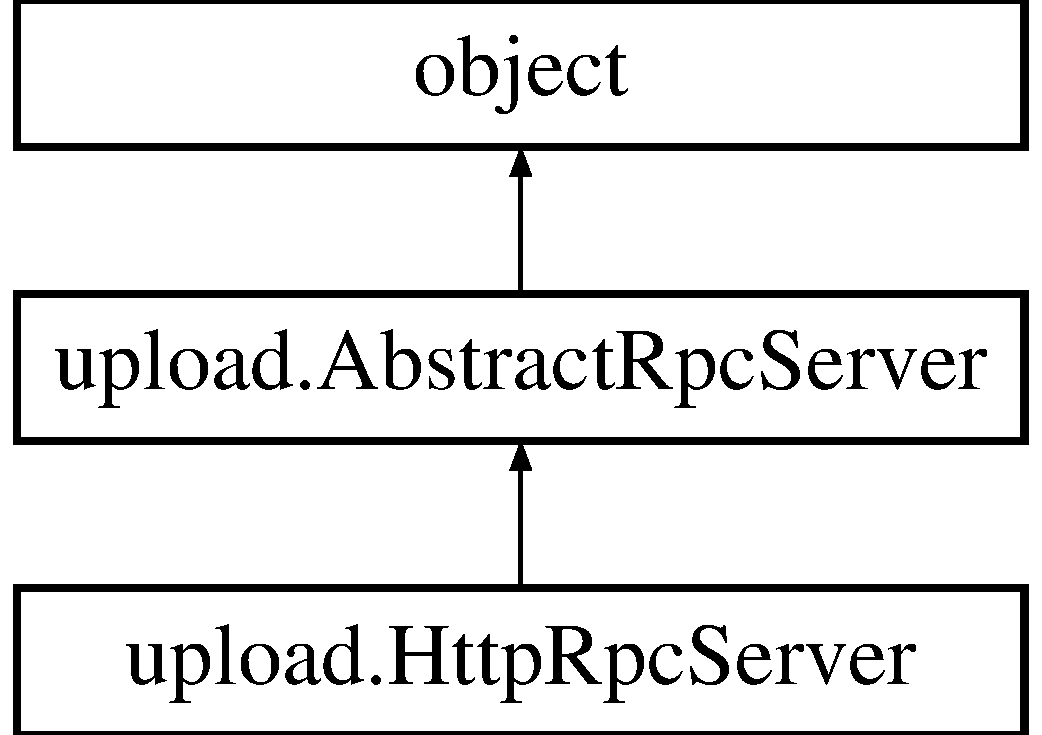
\includegraphics[height=3.000000cm]{classupload_1_1_abstract_rpc_server}
\end{center}
\end{figure}
\subsection*{Public Member Functions}
\begin{DoxyCompactItemize}
\item 
def \mbox{\hyperlink{classupload_1_1_abstract_rpc_server_a3f6bc1bd16b52bd5a5c33a1fedeef2d0}{\+\_\+\+\_\+init\+\_\+\+\_\+}} (self, host, auth\+\_\+function, host\+\_\+override=None, extra\+\_\+headers=\{\}, save\+\_\+cookies=False)
\item 
def \mbox{\hyperlink{classupload_1_1_abstract_rpc_server_ac1b913f8bd00da4741c47ab49ea94cb5}{Send}} (self, request\+\_\+path, payload=None, content\+\_\+type=\char`\"{}application/octet-\/stream\char`\"{}, timeout=None, kwargs)
\end{DoxyCompactItemize}
\subsection*{Public Attributes}
\begin{DoxyCompactItemize}
\item 
\mbox{\Hypertarget{classupload_1_1_abstract_rpc_server_ab7188d827e2faddcf970f524f5856192}\label{classupload_1_1_abstract_rpc_server_ab7188d827e2faddcf970f524f5856192}} 
{\bfseries host}
\item 
\mbox{\Hypertarget{classupload_1_1_abstract_rpc_server_a783a4a7e4ffb776a57a3f267300a213b}\label{classupload_1_1_abstract_rpc_server_a783a4a7e4ffb776a57a3f267300a213b}} 
{\bfseries host\+\_\+override}
\item 
\mbox{\Hypertarget{classupload_1_1_abstract_rpc_server_aee0090a3bcf07b913a7dd596a5dabb8f}\label{classupload_1_1_abstract_rpc_server_aee0090a3bcf07b913a7dd596a5dabb8f}} 
{\bfseries auth\+\_\+function}
\item 
\mbox{\Hypertarget{classupload_1_1_abstract_rpc_server_a692955750c802e461c6336d3000cd365}\label{classupload_1_1_abstract_rpc_server_a692955750c802e461c6336d3000cd365}} 
{\bfseries authenticated}
\item 
\mbox{\Hypertarget{classupload_1_1_abstract_rpc_server_adbbf0109afc13d58d7815fa143cb779f}\label{classupload_1_1_abstract_rpc_server_adbbf0109afc13d58d7815fa143cb779f}} 
{\bfseries extra\+\_\+headers}
\item 
\mbox{\Hypertarget{classupload_1_1_abstract_rpc_server_affe342205c4647d41b127f5a5634858b}\label{classupload_1_1_abstract_rpc_server_affe342205c4647d41b127f5a5634858b}} 
{\bfseries save\+\_\+cookies}
\item 
\mbox{\Hypertarget{classupload_1_1_abstract_rpc_server_aa931446476e0e86f3ade7fef0a0aea5a}\label{classupload_1_1_abstract_rpc_server_aa931446476e0e86f3ade7fef0a0aea5a}} 
{\bfseries opener}
\end{DoxyCompactItemize}


\subsection{Detailed Description}
\begin{DoxyVerb}Provides a common interface for a simple RPC server.\end{DoxyVerb}
 

\subsection{Constructor \& Destructor Documentation}
\mbox{\Hypertarget{classupload_1_1_abstract_rpc_server_a3f6bc1bd16b52bd5a5c33a1fedeef2d0}\label{classupload_1_1_abstract_rpc_server_a3f6bc1bd16b52bd5a5c33a1fedeef2d0}} 
\index{upload\+::\+Abstract\+Rpc\+Server@{upload\+::\+Abstract\+Rpc\+Server}!\+\_\+\+\_\+init\+\_\+\+\_\+@{\+\_\+\+\_\+init\+\_\+\+\_\+}}
\index{\+\_\+\+\_\+init\+\_\+\+\_\+@{\+\_\+\+\_\+init\+\_\+\+\_\+}!upload\+::\+Abstract\+Rpc\+Server@{upload\+::\+Abstract\+Rpc\+Server}}
\subsubsection{\texorpdfstring{\+\_\+\+\_\+init\+\_\+\+\_\+()}{\_\_init\_\_()}}
{\footnotesize\ttfamily def upload.\+Abstract\+Rpc\+Server.\+\_\+\+\_\+init\+\_\+\+\_\+ (\begin{DoxyParamCaption}\item[{}]{self,  }\item[{}]{host,  }\item[{}]{auth\+\_\+function,  }\item[{}]{host\+\_\+override = {\ttfamily None},  }\item[{}]{extra\+\_\+headers = {\ttfamily \{\}},  }\item[{}]{save\+\_\+cookies = {\ttfamily False} }\end{DoxyParamCaption})}

\begin{DoxyVerb}Creates a new HttpRpcServer.

Args:
  host: The host to send requests to.
  auth_function: A function that takes no arguments and returns an
(email, password) tuple when called. Will be called if authentication
is required.
  host_override: The host header to send to the server (defaults to host).
  extra_headers: A dict of extra headers to append to every request.
  save_cookies: If True, save the authentication cookies to local disk.
If False, use an in-memory cookiejar instead.  Subclasses must
implement this functionality.  Defaults to False.
\end{DoxyVerb}
 

\subsection{Member Function Documentation}
\mbox{\Hypertarget{classupload_1_1_abstract_rpc_server_ac1b913f8bd00da4741c47ab49ea94cb5}\label{classupload_1_1_abstract_rpc_server_ac1b913f8bd00da4741c47ab49ea94cb5}} 
\index{upload\+::\+Abstract\+Rpc\+Server@{upload\+::\+Abstract\+Rpc\+Server}!Send@{Send}}
\index{Send@{Send}!upload\+::\+Abstract\+Rpc\+Server@{upload\+::\+Abstract\+Rpc\+Server}}
\subsubsection{\texorpdfstring{Send()}{Send()}}
{\footnotesize\ttfamily def upload.\+Abstract\+Rpc\+Server.\+Send (\begin{DoxyParamCaption}\item[{}]{self,  }\item[{}]{request\+\_\+path,  }\item[{}]{payload = {\ttfamily None},  }\item[{}]{content\+\_\+type = {\ttfamily \char`\"{}application/octet-\/stream\char`\"{}},  }\item[{}]{timeout = {\ttfamily None},  }\item[{}]{kwargs }\end{DoxyParamCaption})}

\begin{DoxyVerb}Sends an RPC and returns the response.

Args:
  request_path: The path to send the request to, eg /api/appversion/create.
  payload: The body of the request, or None to send an empty request.
  content_type: The Content-Type header to use.
  timeout: timeout in seconds; default None i.e. no timeout.
(Note: for large requests on OS X, the timeout doesn't work right.)
  kwargs: Any keyword arguments are converted into query string parameters.

Returns:
  The response body, as a string.
\end{DoxyVerb}
 

The documentation for this class was generated from the following file\+:\begin{DoxyCompactItemize}
\item 
/\+Users/fjp/git/bachelor/bachelor-\/master\+\_\+updated\+\_\+vfinal/googletest-\/1.\+8.\+0/googletest/scripts/upload.\+py\end{DoxyCompactItemize}

\hypertarget{structstd_1_1tr1_1_1gtest__internal_1_1_add_ref}{}\section{std\+:\+:tr1\+:\+:gtest\+\_\+internal\+:\+:Add\+Ref$<$ T $>$ Struct Template Reference}
\label{structstd_1_1tr1_1_1gtest__internal_1_1_add_ref}\index{std\+::tr1\+::gtest\+\_\+internal\+::\+Add\+Ref$<$ T $>$@{std\+::tr1\+::gtest\+\_\+internal\+::\+Add\+Ref$<$ T $>$}}
\subsection*{Public Types}
\begin{DoxyCompactItemize}
\item 
\mbox{\Hypertarget{structstd_1_1tr1_1_1gtest__internal_1_1_add_ref_a1e5616e414125574c1653e3a1fc68491}\label{structstd_1_1tr1_1_1gtest__internal_1_1_add_ref_a1e5616e414125574c1653e3a1fc68491}} 
typedef T \& {\bfseries type}
\end{DoxyCompactItemize}


The documentation for this struct was generated from the following file\+:\begin{DoxyCompactItemize}
\item 
/\+Users/fjp/git/bachelor/bachelor-\/master\+\_\+updated\+\_\+vfinal/googletest-\/1.\+8.\+0/googletest/include/gtest/internal/gtest-\/tuple.\+h\end{DoxyCompactItemize}

\hypertarget{structstd_1_1tr1_1_1gtest__internal_1_1_add_ref_3_01_t_01_6_01_4}{}\section{std\+:\+:tr1\+:\+:gtest\+\_\+internal\+:\+:Add\+Ref$<$ T \& $>$ Struct Template Reference}
\label{structstd_1_1tr1_1_1gtest__internal_1_1_add_ref_3_01_t_01_6_01_4}\index{std\+::tr1\+::gtest\+\_\+internal\+::\+Add\+Ref$<$ T \& $>$@{std\+::tr1\+::gtest\+\_\+internal\+::\+Add\+Ref$<$ T \& $>$}}
\subsection*{Public Types}
\begin{DoxyCompactItemize}
\item 
\mbox{\Hypertarget{structstd_1_1tr1_1_1gtest__internal_1_1_add_ref_3_01_t_01_6_01_4_a9cb3b0992c2a9e7df42d01fb64c2dc88}\label{structstd_1_1tr1_1_1gtest__internal_1_1_add_ref_3_01_t_01_6_01_4_a9cb3b0992c2a9e7df42d01fb64c2dc88}} 
typedef T \& {\bfseries type}
\end{DoxyCompactItemize}


The documentation for this struct was generated from the following file\+:\begin{DoxyCompactItemize}
\item 
/\+Users/fjp/git/bachelor/bachelor-\/master\+\_\+updated\+\_\+vfinal/googletest-\/1.\+8.\+0/googletest/include/gtest/internal/gtest-\/tuple.\+h\end{DoxyCompactItemize}

\hypertarget{structtesting_1_1internal_1_1_add_reference}{}\section{testing\+:\+:internal\+:\+:Add\+Reference$<$ T $>$ Struct Template Reference}
\label{structtesting_1_1internal_1_1_add_reference}\index{testing\+::internal\+::\+Add\+Reference$<$ T $>$@{testing\+::internal\+::\+Add\+Reference$<$ T $>$}}
\subsection*{Public Types}
\begin{DoxyCompactItemize}
\item 
\mbox{\Hypertarget{structtesting_1_1internal_1_1_add_reference_a2df8dd7c4e41f6390e6e66b1a9a67bb4}\label{structtesting_1_1internal_1_1_add_reference_a2df8dd7c4e41f6390e6e66b1a9a67bb4}} 
typedef T \& {\bfseries type}
\end{DoxyCompactItemize}


The documentation for this struct was generated from the following file\+:\begin{DoxyCompactItemize}
\item 
/\+Users/fjp/git/bachelor/bachelor-\/master\+\_\+updated\+\_\+vfinal/googletest-\/1.\+8.\+0/googletest/include/gtest/internal/gtest-\/internal.\+h\end{DoxyCompactItemize}

\hypertarget{structtesting_1_1internal_1_1_add_reference_3_01_t_01_6_01_4}{}\section{testing\+:\+:internal\+:\+:Add\+Reference$<$ T \& $>$ Struct Template Reference}
\label{structtesting_1_1internal_1_1_add_reference_3_01_t_01_6_01_4}\index{testing\+::internal\+::\+Add\+Reference$<$ T \& $>$@{testing\+::internal\+::\+Add\+Reference$<$ T \& $>$}}
\subsection*{Public Types}
\begin{DoxyCompactItemize}
\item 
\mbox{\Hypertarget{structtesting_1_1internal_1_1_add_reference_3_01_t_01_6_01_4_a93c064cdcdaced0abd167258425e57af}\label{structtesting_1_1internal_1_1_add_reference_3_01_t_01_6_01_4_a93c064cdcdaced0abd167258425e57af}} 
typedef T \& {\bfseries type}
\end{DoxyCompactItemize}


The documentation for this struct was generated from the following file\+:\begin{DoxyCompactItemize}
\item 
/\+Users/fjp/git/bachelor/bachelor-\/master\+\_\+updated\+\_\+vfinal/googletest-\/1.\+8.\+0/googletest/include/gtest/internal/gtest-\/internal.\+h\end{DoxyCompactItemize}

\hypertarget{classtesting_1_1gtest__printers__test_1_1_allows_generic_streaming}{}\section{testing\+:\+:gtest\+\_\+printers\+\_\+test\+:\+:Allows\+Generic\+Streaming Class Reference}
\label{classtesting_1_1gtest__printers__test_1_1_allows_generic_streaming}\index{testing\+::gtest\+\_\+printers\+\_\+test\+::\+Allows\+Generic\+Streaming@{testing\+::gtest\+\_\+printers\+\_\+test\+::\+Allows\+Generic\+Streaming}}


The documentation for this class was generated from the following file\+:\begin{DoxyCompactItemize}
\item 
/\+Users/fjp/git/bachelor/bachelor-\/master\+\_\+updated\+\_\+vfinal/googletest-\/1.\+8.\+0/googletest/test/gtest-\/printers\+\_\+test.\+cc\end{DoxyCompactItemize}

\hypertarget{classtesting_1_1gtest__printers__test_1_1_allows_generic_streaming_and_implicit_conversion_template}{}\section{testing\+:\+:gtest\+\_\+printers\+\_\+test\+:\+:Allows\+Generic\+Streaming\+And\+Implicit\+Conversion\+Template$<$ T $>$ Class Template Reference}
\label{classtesting_1_1gtest__printers__test_1_1_allows_generic_streaming_and_implicit_conversion_template}\index{testing\+::gtest\+\_\+printers\+\_\+test\+::\+Allows\+Generic\+Streaming\+And\+Implicit\+Conversion\+Template$<$ T $>$@{testing\+::gtest\+\_\+printers\+\_\+test\+::\+Allows\+Generic\+Streaming\+And\+Implicit\+Conversion\+Template$<$ T $>$}}
\subsection*{Public Member Functions}
\begin{DoxyCompactItemize}
\item 
\mbox{\Hypertarget{classtesting_1_1gtest__printers__test_1_1_allows_generic_streaming_and_implicit_conversion_template_af5f8ea44d7d86283b4c004a994ddd7f9}\label{classtesting_1_1gtest__printers__test_1_1_allows_generic_streaming_and_implicit_conversion_template_af5f8ea44d7d86283b4c004a994ddd7f9}} 
{\bfseries operator bool} () const
\end{DoxyCompactItemize}


The documentation for this class was generated from the following file\+:\begin{DoxyCompactItemize}
\item 
/\+Users/fjp/git/bachelor/bachelor-\/master\+\_\+updated\+\_\+vfinal/googletest-\/1.\+8.\+0/googletest/test/gtest-\/printers\+\_\+test.\+cc\end{DoxyCompactItemize}

\hypertarget{classtesting_1_1gtest__printers__test_1_1_allows_generic_streaming_template}{}\section{testing\+:\+:gtest\+\_\+printers\+\_\+test\+:\+:Allows\+Generic\+Streaming\+Template$<$ T $>$ Class Template Reference}
\label{classtesting_1_1gtest__printers__test_1_1_allows_generic_streaming_template}\index{testing\+::gtest\+\_\+printers\+\_\+test\+::\+Allows\+Generic\+Streaming\+Template$<$ T $>$@{testing\+::gtest\+\_\+printers\+\_\+test\+::\+Allows\+Generic\+Streaming\+Template$<$ T $>$}}


The documentation for this class was generated from the following file\+:\begin{DoxyCompactItemize}
\item 
/\+Users/fjp/git/bachelor/bachelor-\/master\+\_\+updated\+\_\+vfinal/googletest-\/1.\+8.\+0/googletest/test/gtest-\/printers\+\_\+test.\+cc\end{DoxyCompactItemize}

\hypertarget{classtesting_1_1internal_1_1_assert_helper}{}\section{testing\+:\+:internal\+:\+:Assert\+Helper Class Reference}
\label{classtesting_1_1internal_1_1_assert_helper}\index{testing\+::internal\+::\+Assert\+Helper@{testing\+::internal\+::\+Assert\+Helper}}
\subsection*{Public Member Functions}
\begin{DoxyCompactItemize}
\item 
\mbox{\Hypertarget{classtesting_1_1internal_1_1_assert_helper_ac2c9334518fd4087189b4505567a3c90}\label{classtesting_1_1internal_1_1_assert_helper_ac2c9334518fd4087189b4505567a3c90}} 
{\bfseries Assert\+Helper} (Test\+Part\+Result\+::\+Type type, const char $\ast$file, int line, const char $\ast$message)
\item 
\mbox{\Hypertarget{classtesting_1_1internal_1_1_assert_helper_a97bf22d786131ab7baa86b97a27aeb4d}\label{classtesting_1_1internal_1_1_assert_helper_a97bf22d786131ab7baa86b97a27aeb4d}} 
void {\bfseries operator=} (const \mbox{\hyperlink{classtesting_1_1_message}{Message}} \&message) const
\end{DoxyCompactItemize}


The documentation for this class was generated from the following files\+:\begin{DoxyCompactItemize}
\item 
/\+Users/fjp/git/bachelor/bachelor-\/master\+\_\+updated\+\_\+vfinal/googletest-\/1.\+8.\+0/googletest/include/gtest/gtest.\+h\item 
/\+Users/fjp/git/bachelor/bachelor-\/master\+\_\+updated\+\_\+vfinal/googletest-\/1.\+8.\+0/googletest/src/gtest.\+cc\end{DoxyCompactItemize}

\hypertarget{classtesting_1_1_assertion_result}{}\section{testing\+:\+:Assertion\+Result Class Reference}
\label{classtesting_1_1_assertion_result}\index{testing\+::\+Assertion\+Result@{testing\+::\+Assertion\+Result}}
\subsection*{Public Member Functions}
\begin{DoxyCompactItemize}
\item 
\mbox{\Hypertarget{classtesting_1_1_assertion_result_a27788116f03f90aec4daf592fd809ead}\label{classtesting_1_1_assertion_result_a27788116f03f90aec4daf592fd809ead}} 
{\bfseries Assertion\+Result} (const \mbox{\hyperlink{classtesting_1_1_assertion_result}{Assertion\+Result}} \&other)
\item 
\mbox{\Hypertarget{classtesting_1_1_assertion_result_a9b8d1d6d0a979d0769ed4ff97d06c4e3}\label{classtesting_1_1_assertion_result_a9b8d1d6d0a979d0769ed4ff97d06c4e3}} 
{\footnotesize template$<$typename T $>$ }\\{\bfseries Assertion\+Result} (const T \&success, typename \mbox{\hyperlink{structtesting_1_1internal_1_1_enable_if}{internal\+::\+Enable\+If}}$<$ !\mbox{\hyperlink{classtesting_1_1internal_1_1_implicitly_convertible}{internal\+::\+Implicitly\+Convertible}}$<$ T, \mbox{\hyperlink{classtesting_1_1_assertion_result}{Assertion\+Result}} $>$\+::value $>$\+::type $\ast$=N\+U\+LL)
\item 
\mbox{\Hypertarget{classtesting_1_1_assertion_result_aad9274c7b69eda67eb9306963a790839}\label{classtesting_1_1_assertion_result_aad9274c7b69eda67eb9306963a790839}} 
\mbox{\hyperlink{classtesting_1_1_assertion_result}{Assertion\+Result}} \& {\bfseries operator=} (\mbox{\hyperlink{classtesting_1_1_assertion_result}{Assertion\+Result}} other)
\item 
\mbox{\Hypertarget{classtesting_1_1_assertion_result_ab3f34b1623c82762ef4a8f52b535159c}\label{classtesting_1_1_assertion_result_ab3f34b1623c82762ef4a8f52b535159c}} 
{\bfseries operator bool} () const
\item 
\mbox{\Hypertarget{classtesting_1_1_assertion_result_a5b0784686a756660ac8dfe528d89386b}\label{classtesting_1_1_assertion_result_a5b0784686a756660ac8dfe528d89386b}} 
\mbox{\hyperlink{classtesting_1_1_assertion_result}{Assertion\+Result}} {\bfseries operator!} () const
\item 
\mbox{\Hypertarget{classtesting_1_1_assertion_result_a33c14dafd28e3393c841e03f4b70a017}\label{classtesting_1_1_assertion_result_a33c14dafd28e3393c841e03f4b70a017}} 
const char $\ast$ {\bfseries message} () const
\item 
\mbox{\Hypertarget{classtesting_1_1_assertion_result_aa38908d5a48c912434a80c8725f52583}\label{classtesting_1_1_assertion_result_aa38908d5a48c912434a80c8725f52583}} 
const char $\ast$ {\bfseries failure\+\_\+message} () const
\item 
\mbox{\Hypertarget{classtesting_1_1_assertion_result_a3230efa81aafe7c61f5fb878cfa39e91}\label{classtesting_1_1_assertion_result_a3230efa81aafe7c61f5fb878cfa39e91}} 
{\footnotesize template$<$typename T $>$ }\\\mbox{\hyperlink{classtesting_1_1_assertion_result}{Assertion\+Result}} \& {\bfseries operator$<$$<$} (const T \&value)
\item 
\mbox{\Hypertarget{classtesting_1_1_assertion_result_a43ae8a260843ce2ff3dc9af262672b8b}\label{classtesting_1_1_assertion_result_a43ae8a260843ce2ff3dc9af262672b8b}} 
\mbox{\hyperlink{classtesting_1_1_assertion_result}{Assertion\+Result}} \& {\bfseries operator$<$$<$} (\+::std\+::ostream \&($\ast$basic\+\_\+manipulator)(\+::std\+::ostream \&stream))
\end{DoxyCompactItemize}


The documentation for this class was generated from the following files\+:\begin{DoxyCompactItemize}
\item 
/\+Users/fjp/git/bachelor/bachelor-\/master\+\_\+updated\+\_\+vfinal/googletest-\/1.\+8.\+0/googletest/include/gtest/gtest.\+h\item 
/\+Users/fjp/git/bachelor/bachelor-\/master\+\_\+updated\+\_\+vfinal/googletest-\/1.\+8.\+0/googletest/src/gtest.\+cc\end{DoxyCompactItemize}

\hypertarget{classmy__namespace_1_1testing_1_1_assertion_result}{}\section{my\+\_\+namespace\+:\+:testing\+:\+:Assertion\+Result Class Reference}
\label{classmy__namespace_1_1testing_1_1_assertion_result}\index{my\+\_\+namespace\+::testing\+::\+Assertion\+Result@{my\+\_\+namespace\+::testing\+::\+Assertion\+Result}}


The documentation for this class was generated from the following file\+:\begin{DoxyCompactItemize}
\item 
/\+Users/fjp/git/bachelor/bachelor-\/master\+\_\+updated\+\_\+vfinal/googletest-\/1.\+8.\+0/googletest/test/gtest\+\_\+unittest.\+cc\end{DoxyCompactItemize}

\hypertarget{class_bar_environment}{}\section{Bar\+Environment Class Reference}
\label{class_bar_environment}\index{Bar\+Environment@{Bar\+Environment}}
Inheritance diagram for Bar\+Environment\+:\begin{figure}[H]
\begin{center}
\leavevmode
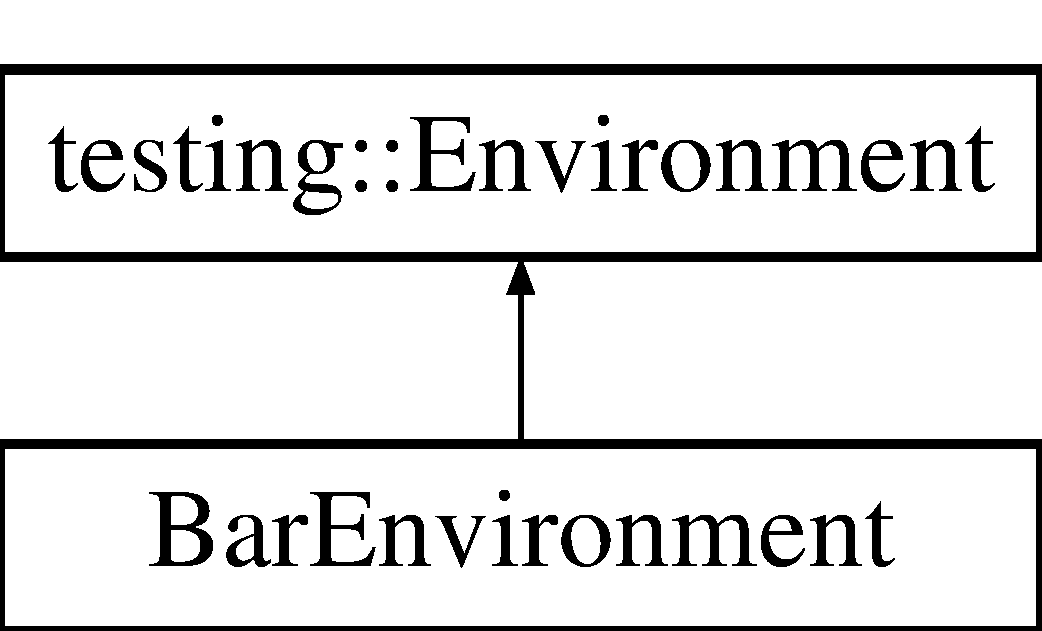
\includegraphics[height=2.000000cm]{class_bar_environment}
\end{center}
\end{figure}
\subsection*{Public Member Functions}
\begin{DoxyCompactItemize}
\item 
\mbox{\Hypertarget{class_bar_environment_a88e17c5dd1dcea7a4538f2f3c6bf7bdd}\label{class_bar_environment_a88e17c5dd1dcea7a4538f2f3c6bf7bdd}} 
virtual void {\bfseries Set\+Up} ()
\item 
\mbox{\Hypertarget{class_bar_environment_a384f951da72a2a18bb0c2b3506376b09}\label{class_bar_environment_a384f951da72a2a18bb0c2b3506376b09}} 
virtual void {\bfseries Tear\+Down} ()
\end{DoxyCompactItemize}


The documentation for this class was generated from the following file\+:\begin{DoxyCompactItemize}
\item 
/\+Users/fjp/git/bachelor/bachelor-\/master\+\_\+updated\+\_\+vfinal/googletest-\/1.\+8.\+0/googletest/test/gtest\+\_\+output\+\_\+test\+\_\+.\+cc\end{DoxyCompactItemize}

\hypertarget{class_base}{}\section{Base Class Reference}
\label{class_base}\index{Base@{Base}}
Inheritance diagram for Base\+:\begin{figure}[H]
\begin{center}
\leavevmode
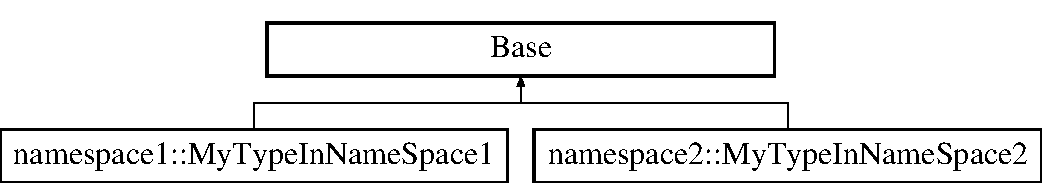
\includegraphics[height=2.000000cm]{class_base}
\end{center}
\end{figure}
\subsection*{Public Member Functions}
\begin{DoxyCompactItemize}
\item 
\mbox{\Hypertarget{class_base_a1d5f3fb92f8cbc687705785bdc6abd18}\label{class_base_a1d5f3fb92f8cbc687705785bdc6abd18}} 
{\bfseries Base} (int an\+\_\+x)
\item 
\mbox{\Hypertarget{class_base_a779fd2b157ebd763b15383d96047e07c}\label{class_base_a779fd2b157ebd763b15383d96047e07c}} 
int {\bfseries x} () const
\end{DoxyCompactItemize}


The documentation for this class was generated from the following file\+:\begin{DoxyCompactItemize}
\item 
/\+Users/fjp/git/bachelor/bachelor-\/master\+\_\+updated\+\_\+vfinal/googletest-\/1.\+8.\+0/googletest/test/gtest\+\_\+unittest.\+cc\end{DoxyCompactItemize}

\hypertarget{classtesting_1_1internal_1_1_base}{}\section{testing\+:\+:internal\+:\+:Base Class Reference}
\label{classtesting_1_1internal_1_1_base}\index{testing\+::internal\+::\+Base@{testing\+::internal\+::\+Base}}
Inheritance diagram for testing\+:\+:internal\+:\+:Base\+:\begin{figure}[H]
\begin{center}
\leavevmode
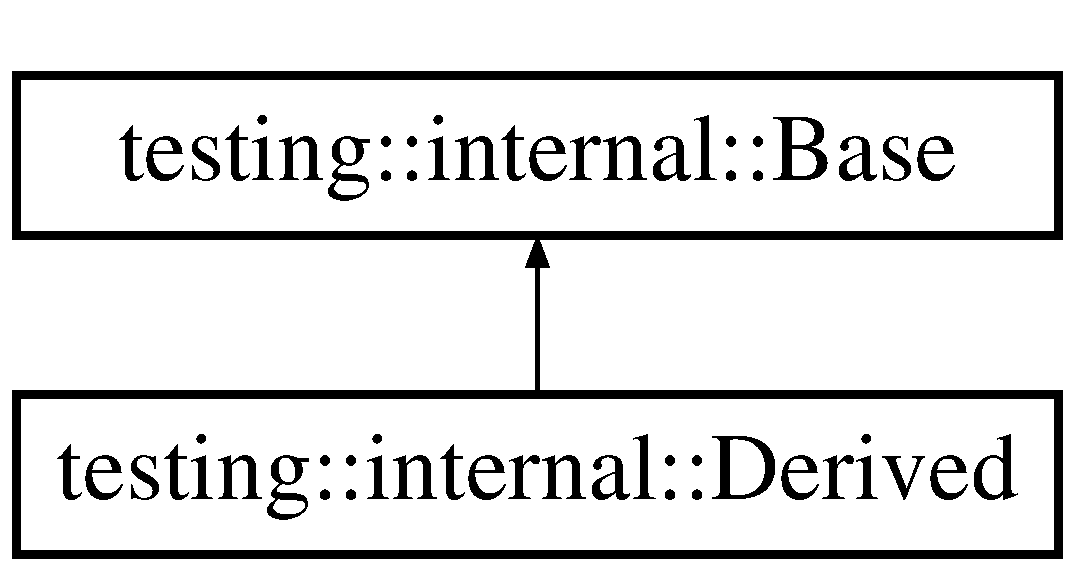
\includegraphics[height=2.000000cm]{classtesting_1_1internal_1_1_base}
\end{center}
\end{figure}
\subsection*{Public Member Functions}
\begin{DoxyCompactItemize}
\item 
\mbox{\Hypertarget{classtesting_1_1internal_1_1_base_a255d105410a1eeb5f4690c9c8cd8e104}\label{classtesting_1_1internal_1_1_base_a255d105410a1eeb5f4690c9c8cd8e104}} 
{\bfseries Base} (int n)
\item 
\mbox{\Hypertarget{classtesting_1_1internal_1_1_base_a7ddba6221b56613be545544b7ef6214c}\label{classtesting_1_1internal_1_1_base_a7ddba6221b56613be545544b7ef6214c}} 
int {\bfseries member} ()
\end{DoxyCompactItemize}


The documentation for this class was generated from the following file\+:\begin{DoxyCompactItemize}
\item 
/\+Users/fjp/git/bachelor/bachelor-\/master\+\_\+updated\+\_\+vfinal/googletest-\/1.\+8.\+0/googletest/test/gtest-\/port\+\_\+test.\+cc\end{DoxyCompactItemize}

\hypertarget{structtesting_1_1gtest__printers__test_1_1_big}{}\section{testing\+:\+:gtest\+\_\+printers\+\_\+test\+:\+:Big Struct Reference}
\label{structtesting_1_1gtest__printers__test_1_1_big}\index{testing\+::gtest\+\_\+printers\+\_\+test\+::\+Big@{testing\+::gtest\+\_\+printers\+\_\+test\+::\+Big}}
\subsection*{Public Attributes}
\begin{DoxyCompactItemize}
\item 
\mbox{\Hypertarget{structtesting_1_1gtest__printers__test_1_1_big_a863911a8ec5c3bbe79c44d399f1de61f}\label{structtesting_1_1gtest__printers__test_1_1_big_a863911a8ec5c3bbe79c44d399f1de61f}} 
char {\bfseries array} \mbox{[}257\mbox{]}
\end{DoxyCompactItemize}


The documentation for this struct was generated from the following file\+:\begin{DoxyCompactItemize}
\item 
/\+Users/fjp/git/bachelor/bachelor-\/master\+\_\+updated\+\_\+vfinal/googletest-\/1.\+8.\+0/googletest/test/gtest-\/printers\+\_\+test.\+cc\end{DoxyCompactItemize}

\hypertarget{class_biggest_int_convertible}{}\section{Biggest\+Int\+Convertible Class Reference}
\label{class_biggest_int_convertible}\index{Biggest\+Int\+Convertible@{Biggest\+Int\+Convertible}}
\subsection*{Public Member Functions}
\begin{DoxyCompactItemize}
\item 
\mbox{\Hypertarget{class_biggest_int_convertible_aa3dc4bbff87d412758b9adbefa19c6d0}\label{class_biggest_int_convertible_aa3dc4bbff87d412758b9adbefa19c6d0}} 
{\bfseries operator\+::testing\+::internal\+::\+Biggest\+Int} () const
\end{DoxyCompactItemize}


The documentation for this class was generated from the following file\+:\begin{DoxyCompactItemize}
\item 
/\+Users/fjp/git/bachelor/bachelor-\/master\+\_\+updated\+\_\+vfinal/googletest-\/1.\+8.\+0/googletest/test/gtest-\/printers\+\_\+test.\+cc\end{DoxyCompactItemize}

\hypertarget{structvisualizer_1_1_bitmap}{}\section{visualizer\+:\+:Bitmap Struct Reference}
\label{structvisualizer_1_1_bitmap}\index{visualizer\+::\+Bitmap@{visualizer\+::\+Bitmap}}


Collaboration diagram for visualizer\+:\+:Bitmap\+:
\nopagebreak
\begin{figure}[H]
\begin{center}
\leavevmode
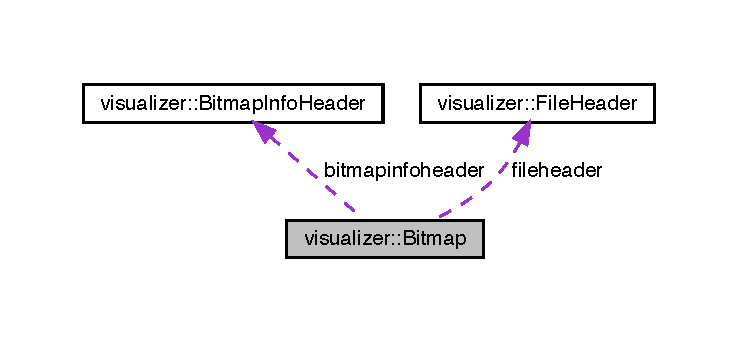
\includegraphics[width=350pt]{structvisualizer_1_1_bitmap__coll__graph}
\end{center}
\end{figure}
\subsection*{Public Attributes}
\begin{DoxyCompactItemize}
\item 
\mbox{\Hypertarget{structvisualizer_1_1_bitmap_a35cd50ab96ca92a2f3cc92fbec0ccef0}\label{structvisualizer_1_1_bitmap_a35cd50ab96ca92a2f3cc92fbec0ccef0}} 
\mbox{\hyperlink{structvisualizer_1_1_file_header}{File\+Header}} {\bfseries fileheader}
\item 
\mbox{\Hypertarget{structvisualizer_1_1_bitmap_ae321d14404bf8daff08333b6b2858603}\label{structvisualizer_1_1_bitmap_ae321d14404bf8daff08333b6b2858603}} 
\mbox{\hyperlink{structvisualizer_1_1_bitmap_info_header}{Bitmap\+Info\+Header}} {\bfseries bitmapinfoheader}
\end{DoxyCompactItemize}


The documentation for this struct was generated from the following file\+:\begin{DoxyCompactItemize}
\item 
/\+Users/fjp/git/bachelor/visualizer/visualizer.\+cpp\end{DoxyCompactItemize}

\hypertarget{structvisualizer_1_1_bitmap_info_header}{}\section{visualizer\+:\+:Bitmap\+Info\+Header Struct Reference}
\label{structvisualizer_1_1_bitmap_info_header}\index{visualizer\+::\+Bitmap\+Info\+Header@{visualizer\+::\+Bitmap\+Info\+Header}}
\subsection*{Public Attributes}
\begin{DoxyCompactItemize}
\item 
\mbox{\Hypertarget{structvisualizer_1_1_bitmap_info_header_aa948614dcf785eb73fc5f8e6d167cffe}\label{structvisualizer_1_1_bitmap_info_header_aa948614dcf785eb73fc5f8e6d167cffe}} 
uint32\+\_\+t {\bfseries dibheadersize}
\item 
\mbox{\Hypertarget{structvisualizer_1_1_bitmap_info_header_adbdbe8eb51d35287f34011bb807e2cc9}\label{structvisualizer_1_1_bitmap_info_header_adbdbe8eb51d35287f34011bb807e2cc9}} 
uint32\+\_\+t {\bfseries width}
\item 
\mbox{\Hypertarget{structvisualizer_1_1_bitmap_info_header_a690035c63f73bca8e8f7dec8c34e57eb}\label{structvisualizer_1_1_bitmap_info_header_a690035c63f73bca8e8f7dec8c34e57eb}} 
uint32\+\_\+t {\bfseries height}
\item 
\mbox{\Hypertarget{structvisualizer_1_1_bitmap_info_header_a388f28427be89d01501baf6684334279}\label{structvisualizer_1_1_bitmap_info_header_a388f28427be89d01501baf6684334279}} 
uint16\+\_\+t {\bfseries planes}
\item 
\mbox{\Hypertarget{structvisualizer_1_1_bitmap_info_header_aae99ff5c9e392f5b9071e71e96214037}\label{structvisualizer_1_1_bitmap_info_header_aae99ff5c9e392f5b9071e71e96214037}} 
uint16\+\_\+t {\bfseries bitsperpixel}
\item 
\mbox{\Hypertarget{structvisualizer_1_1_bitmap_info_header_a96381aa9deebf9a89a47ccf84e686b17}\label{structvisualizer_1_1_bitmap_info_header_a96381aa9deebf9a89a47ccf84e686b17}} 
uint32\+\_\+t {\bfseries compression}
\item 
\mbox{\Hypertarget{structvisualizer_1_1_bitmap_info_header_a5f8c0e9eae60a612efb52b33cd52e3e1}\label{structvisualizer_1_1_bitmap_info_header_a5f8c0e9eae60a612efb52b33cd52e3e1}} 
uint32\+\_\+t {\bfseries imagesize}
\item 
\mbox{\Hypertarget{structvisualizer_1_1_bitmap_info_header_a5cc22a4fff1707a47ae60b2ac1f6be53}\label{structvisualizer_1_1_bitmap_info_header_a5cc22a4fff1707a47ae60b2ac1f6be53}} 
uint32\+\_\+t {\bfseries ypixelpermeter}
\item 
\mbox{\Hypertarget{structvisualizer_1_1_bitmap_info_header_a55f795ae6a8f855cbc3a9cad8d69b091}\label{structvisualizer_1_1_bitmap_info_header_a55f795ae6a8f855cbc3a9cad8d69b091}} 
uint32\+\_\+t {\bfseries xpixelpermeter}
\item 
\mbox{\Hypertarget{structvisualizer_1_1_bitmap_info_header_a828bf1dbc3f160913e1a835ad007056b}\label{structvisualizer_1_1_bitmap_info_header_a828bf1dbc3f160913e1a835ad007056b}} 
uint32\+\_\+t {\bfseries numcolorspallette}
\item 
\mbox{\Hypertarget{structvisualizer_1_1_bitmap_info_header_a3569cfb8679eec61adfa907348e5c898}\label{structvisualizer_1_1_bitmap_info_header_a3569cfb8679eec61adfa907348e5c898}} 
uint32\+\_\+t {\bfseries mostimpcolor}
\end{DoxyCompactItemize}


The documentation for this struct was generated from the following file\+:\begin{DoxyCompactItemize}
\item 
/\+Users/fjp/git/bachelor/bachelor-\/master\+\_\+updated\+\_\+vfinal/visualizer/visualizer.\+cpp\end{DoxyCompactItemize}

\hypertarget{struct_bool}{}\section{Bool Struct Reference}
\label{struct_bool}\index{Bool@{Bool}}
\subsection*{Public Member Functions}
\begin{DoxyCompactItemize}
\item 
\mbox{\Hypertarget{struct_bool_a03dfd4851b13abb29414887fcada7fca}\label{struct_bool_a03dfd4851b13abb29414887fcada7fca}} 
{\bfseries Bool} (int val)
\item 
\mbox{\Hypertarget{struct_bool_a7baecbc58992eb06157fbbbaa560be0b}\label{struct_bool_a7baecbc58992eb06157fbbbaa560be0b}} 
bool {\bfseries operator$>$} (int n) const
\item 
\mbox{\Hypertarget{struct_bool_a6f4ecdec19082e896cffce66e6b6e7cc}\label{struct_bool_a6f4ecdec19082e896cffce66e6b6e7cc}} 
\mbox{\hyperlink{struct_bool}{Bool}} {\bfseries operator+} (const \mbox{\hyperlink{struct_bool}{Bool}} \&rhs) const
\item 
\mbox{\Hypertarget{struct_bool_afe799a4977c5ebe4c215d5d4ebd77adb}\label{struct_bool_afe799a4977c5ebe4c215d5d4ebd77adb}} 
bool {\bfseries operator==} (const \mbox{\hyperlink{struct_bool}{Bool}} \&rhs) const
\end{DoxyCompactItemize}
\subsection*{Public Attributes}
\begin{DoxyCompactItemize}
\item 
\mbox{\Hypertarget{struct_bool_a16be863c269f988cdcbe59f9d846a141}\label{struct_bool_a16be863c269f988cdcbe59f9d846a141}} 
bool {\bfseries value}
\end{DoxyCompactItemize}


The documentation for this struct was generated from the following file\+:\begin{DoxyCompactItemize}
\item 
/\+Users/fjp/git/bachelor/bachelor-\/master\+\_\+updated\+\_\+vfinal/googletest-\/1.\+8.\+0/googletest/test/gtest\+\_\+pred\+\_\+impl\+\_\+unittest.\+cc\end{DoxyCompactItemize}

\hypertarget{structtesting_1_1internal_1_1bool__constant}{}\section{testing\+:\+:internal\+:\+:bool\+\_\+constant$<$ bool\+\_\+value $>$ Struct Template Reference}
\label{structtesting_1_1internal_1_1bool__constant}\index{testing\+::internal\+::bool\+\_\+constant$<$ bool\+\_\+value $>$@{testing\+::internal\+::bool\+\_\+constant$<$ bool\+\_\+value $>$}}
Inheritance diagram for testing\+:\+:internal\+:\+:bool\+\_\+constant$<$ bool\+\_\+value $>$\+:\begin{figure}[H]
\begin{center}
\leavevmode
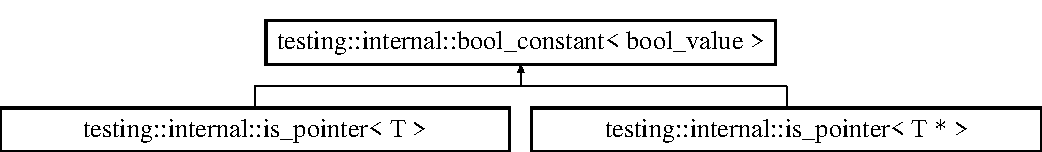
\includegraphics[height=2.000000cm]{structtesting_1_1internal_1_1bool__constant}
\end{center}
\end{figure}
\subsection*{Public Types}
\begin{DoxyCompactItemize}
\item 
\mbox{\Hypertarget{structtesting_1_1internal_1_1bool__constant_aba6d09ecf7eecea6c93480f0d627a167}\label{structtesting_1_1internal_1_1bool__constant_aba6d09ecf7eecea6c93480f0d627a167}} 
typedef \mbox{\hyperlink{structtesting_1_1internal_1_1bool__constant}{bool\+\_\+constant}}$<$ bool\+\_\+value $>$ {\bfseries type}
\end{DoxyCompactItemize}
\subsection*{Static Public Attributes}
\begin{DoxyCompactItemize}
\item 
\mbox{\Hypertarget{structtesting_1_1internal_1_1bool__constant_a499fba6576296b04d99690a486424b32}\label{structtesting_1_1internal_1_1bool__constant_a499fba6576296b04d99690a486424b32}} 
static const bool {\bfseries value} = bool\+\_\+value
\end{DoxyCompactItemize}


The documentation for this struct was generated from the following file\+:\begin{DoxyCompactItemize}
\item 
/\+Users/fjp/git/bachelor/bachelor-\/master\+\_\+updated\+\_\+vfinal/googletest-\/1.\+8.\+0/googletest/include/gtest/internal/gtest-\/port.\+h\end{DoxyCompactItemize}

\hypertarget{structstd_1_1tr1_1_1gtest__internal_1_1_by_ref}{}\section{std\+:\+:tr1\+:\+:gtest\+\_\+internal\+:\+:By\+Ref$<$ T $>$ Struct Template Reference}
\label{structstd_1_1tr1_1_1gtest__internal_1_1_by_ref}\index{std\+::tr1\+::gtest\+\_\+internal\+::\+By\+Ref$<$ T $>$@{std\+::tr1\+::gtest\+\_\+internal\+::\+By\+Ref$<$ T $>$}}
\subsection*{Public Types}
\begin{DoxyCompactItemize}
\item 
\mbox{\Hypertarget{structstd_1_1tr1_1_1gtest__internal_1_1_by_ref_ac42ad942ee1cfa86b2abcce9b88ac10e}\label{structstd_1_1tr1_1_1gtest__internal_1_1_by_ref_ac42ad942ee1cfa86b2abcce9b88ac10e}} 
typedef const T \& {\bfseries type}
\end{DoxyCompactItemize}


The documentation for this struct was generated from the following file\+:\begin{DoxyCompactItemize}
\item 
/\+Users/fjp/git/bachelor/bachelor-\/master\+\_\+updated\+\_\+vfinal/googletest-\/1.\+8.\+0/googletest/include/gtest/internal/gtest-\/tuple.\+h\end{DoxyCompactItemize}

\hypertarget{structstd_1_1tr1_1_1gtest__internal_1_1_by_ref_3_01_t_01_6_01_4}{}\section{std\+:\+:tr1\+:\+:gtest\+\_\+internal\+:\+:By\+Ref$<$ T \& $>$ Struct Template Reference}
\label{structstd_1_1tr1_1_1gtest__internal_1_1_by_ref_3_01_t_01_6_01_4}\index{std\+::tr1\+::gtest\+\_\+internal\+::\+By\+Ref$<$ T \& $>$@{std\+::tr1\+::gtest\+\_\+internal\+::\+By\+Ref$<$ T \& $>$}}
\subsection*{Public Types}
\begin{DoxyCompactItemize}
\item 
\mbox{\Hypertarget{structstd_1_1tr1_1_1gtest__internal_1_1_by_ref_3_01_t_01_6_01_4_a512382574dbdd736320d68e313801122}\label{structstd_1_1tr1_1_1gtest__internal_1_1_by_ref_3_01_t_01_6_01_4_a512382574dbdd736320d68e313801122}} 
typedef T \& {\bfseries type}
\end{DoxyCompactItemize}


The documentation for this struct was generated from the following file\+:\begin{DoxyCompactItemize}
\item 
/\+Users/fjp/git/bachelor/bachelor-\/master\+\_\+updated\+\_\+vfinal/googletest-\/1.\+8.\+0/googletest/include/gtest/internal/gtest-\/tuple.\+h\end{DoxyCompactItemize}

\hypertarget{classtesting_1_1internal_1_1_castable}{}\section{testing\+:\+:internal\+:\+:Castable Class Reference}
\label{classtesting_1_1internal_1_1_castable}\index{testing\+::internal\+::\+Castable@{testing\+::internal\+::\+Castable}}
\subsection*{Public Member Functions}
\begin{DoxyCompactItemize}
\item 
\mbox{\Hypertarget{classtesting_1_1internal_1_1_castable_a705d519a227d38ff5c174905316f62c4}\label{classtesting_1_1internal_1_1_castable_a705d519a227d38ff5c174905316f62c4}} 
{\bfseries Castable} (bool $\ast$converted)
\item 
\mbox{\Hypertarget{classtesting_1_1internal_1_1_castable_ac60b2e7885f3b09defb829eddaa0afd9}\label{classtesting_1_1internal_1_1_castable_ac60b2e7885f3b09defb829eddaa0afd9}} 
{\bfseries operator Base} ()
\end{DoxyCompactItemize}


The documentation for this class was generated from the following file\+:\begin{DoxyCompactItemize}
\item 
/\+Users/fjp/git/bachelor/bachelor-\/master\+\_\+updated\+\_\+vfinal/googletest-\/1.\+8.\+0/googletest/test/gtest-\/port\+\_\+test.\+cc\end{DoxyCompactItemize}

\hypertarget{classgtest__catch__exceptions__test_1_1_catch_cxx_exceptions_test}{}\section{gtest\+\_\+catch\+\_\+exceptions\+\_\+test.\+Catch\+Cxx\+Exceptions\+Test Class Reference}
\label{classgtest__catch__exceptions__test_1_1_catch_cxx_exceptions_test}\index{gtest\+\_\+catch\+\_\+exceptions\+\_\+test.\+Catch\+Cxx\+Exceptions\+Test@{gtest\+\_\+catch\+\_\+exceptions\+\_\+test.\+Catch\+Cxx\+Exceptions\+Test}}
Inheritance diagram for gtest\+\_\+catch\+\_\+exceptions\+\_\+test.\+Catch\+Cxx\+Exceptions\+Test\+:\begin{figure}[H]
\begin{center}
\leavevmode
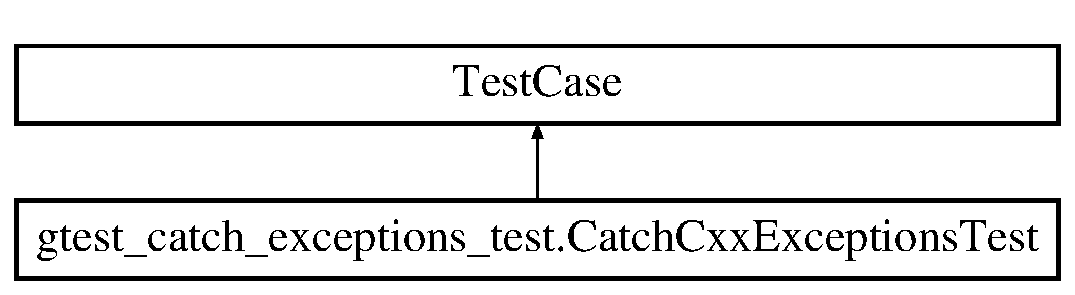
\includegraphics[height=2.000000cm]{classgtest__catch__exceptions__test_1_1_catch_cxx_exceptions_test}
\end{center}
\end{figure}
\subsection*{Public Member Functions}
\begin{DoxyCompactItemize}
\item 
\mbox{\Hypertarget{classgtest__catch__exceptions__test_1_1_catch_cxx_exceptions_test_a7d02a890df0e3990aa107288c21f7dc7}\label{classgtest__catch__exceptions__test_1_1_catch_cxx_exceptions_test_a7d02a890df0e3990aa107288c21f7dc7}} 
def {\bfseries test\+Catches\+Cxx\+Exceptions\+In\+Fixture\+Constructor} (self)
\item 
\mbox{\Hypertarget{classgtest__catch__exceptions__test_1_1_catch_cxx_exceptions_test_a3fe17da71b72c1693fa358f71c6b31be}\label{classgtest__catch__exceptions__test_1_1_catch_cxx_exceptions_test_a3fe17da71b72c1693fa358f71c6b31be}} 
def {\bfseries test\+Catches\+Cxx\+Exceptions\+In\+Fixture\+Destructor} (self)
\item 
\mbox{\Hypertarget{classgtest__catch__exceptions__test_1_1_catch_cxx_exceptions_test_a8e791760b553d92490005deea0812f44}\label{classgtest__catch__exceptions__test_1_1_catch_cxx_exceptions_test_a8e791760b553d92490005deea0812f44}} 
def {\bfseries test\+Catches\+Cxx\+Exceptions\+In\+Set\+Up\+Test\+Case} (self)
\item 
\mbox{\Hypertarget{classgtest__catch__exceptions__test_1_1_catch_cxx_exceptions_test_a56c906c34e689ee016ab1bf14fe5220c}\label{classgtest__catch__exceptions__test_1_1_catch_cxx_exceptions_test_a56c906c34e689ee016ab1bf14fe5220c}} 
def {\bfseries test\+Catches\+Cxx\+Exceptions\+In\+Tear\+Down\+Test\+Case} (self)
\item 
\mbox{\Hypertarget{classgtest__catch__exceptions__test_1_1_catch_cxx_exceptions_test_a6451307941e063bcc3927992c1f2df54}\label{classgtest__catch__exceptions__test_1_1_catch_cxx_exceptions_test_a6451307941e063bcc3927992c1f2df54}} 
def {\bfseries test\+Catches\+Cxx\+Exceptions\+In\+Set\+Up} (self)
\item 
\mbox{\Hypertarget{classgtest__catch__exceptions__test_1_1_catch_cxx_exceptions_test_a40ba50bf018753b7b21ed93ed60e4e1c}\label{classgtest__catch__exceptions__test_1_1_catch_cxx_exceptions_test_a40ba50bf018753b7b21ed93ed60e4e1c}} 
def {\bfseries test\+Catches\+Cxx\+Exceptions\+In\+Tear\+Down} (self)
\item 
\mbox{\Hypertarget{classgtest__catch__exceptions__test_1_1_catch_cxx_exceptions_test_ac73b336590a3d1c242124e9ea5464a42}\label{classgtest__catch__exceptions__test_1_1_catch_cxx_exceptions_test_ac73b336590a3d1c242124e9ea5464a42}} 
def {\bfseries test\+Catches\+Cxx\+Exceptions\+In\+Test\+Body} (self)
\item 
\mbox{\Hypertarget{classgtest__catch__exceptions__test_1_1_catch_cxx_exceptions_test_a922cb0b598034924c19e6695cc9f7513}\label{classgtest__catch__exceptions__test_1_1_catch_cxx_exceptions_test_a922cb0b598034924c19e6695cc9f7513}} 
def {\bfseries test\+Catches\+Non\+Std\+Cxx\+Exceptions} (self)
\item 
\mbox{\Hypertarget{classgtest__catch__exceptions__test_1_1_catch_cxx_exceptions_test_af3a794d5af0b3d72789293531468050a}\label{classgtest__catch__exceptions__test_1_1_catch_cxx_exceptions_test_af3a794d5af0b3d72789293531468050a}} 
def {\bfseries test\+Unhandled\+Cxx\+Exceptions\+Abort\+The\+Program} (self)
\end{DoxyCompactItemize}


\subsection{Detailed Description}
\begin{DoxyVerb}Tests C++ exception-catching behavior.

   Tests in this test case verify that:
   * C++ exceptions are caught and logged as C++ (not SEH) exceptions
   * Exception thrown affect the remainder of the test work flow in the
     expected manner.
\end{DoxyVerb}
 

The documentation for this class was generated from the following file\+:\begin{DoxyCompactItemize}
\item 
/\+Users/fjp/git/bachelor/bachelor-\/master\+\_\+updated\+\_\+vfinal/googletest-\/1.\+8.\+0/googletest/test/gtest\+\_\+catch\+\_\+exceptions\+\_\+test.\+py\end{DoxyCompactItemize}

\hypertarget{classgtest__catch__exceptions__test_1_1_catch_seh_exceptions_test}{}\section{gtest\+\_\+catch\+\_\+exceptions\+\_\+test.\+Catch\+Seh\+Exceptions\+Test Class Reference}
\label{classgtest__catch__exceptions__test_1_1_catch_seh_exceptions_test}\index{gtest\+\_\+catch\+\_\+exceptions\+\_\+test.\+Catch\+Seh\+Exceptions\+Test@{gtest\+\_\+catch\+\_\+exceptions\+\_\+test.\+Catch\+Seh\+Exceptions\+Test}}
Inheritance diagram for gtest\+\_\+catch\+\_\+exceptions\+\_\+test.\+Catch\+Seh\+Exceptions\+Test\+:\begin{figure}[H]
\begin{center}
\leavevmode
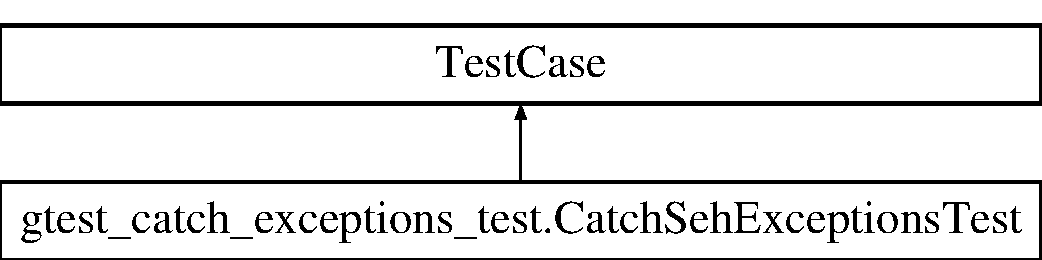
\includegraphics[height=2.000000cm]{classgtest__catch__exceptions__test_1_1_catch_seh_exceptions_test}
\end{center}
\end{figure}
\subsection*{Public Member Functions}
\begin{DoxyCompactItemize}
\item 
\mbox{\Hypertarget{classgtest__catch__exceptions__test_1_1_catch_seh_exceptions_test_a737bbcc64405854aa8e0aea87ca5850b}\label{classgtest__catch__exceptions__test_1_1_catch_seh_exceptions_test_a737bbcc64405854aa8e0aea87ca5850b}} 
def {\bfseries Test\+Seh\+Exceptions} (self, test\+\_\+output)
\item 
\mbox{\Hypertarget{classgtest__catch__exceptions__test_1_1_catch_seh_exceptions_test_a02d06790fb52416a9da6a28b624e9cd9}\label{classgtest__catch__exceptions__test_1_1_catch_seh_exceptions_test_a02d06790fb52416a9da6a28b624e9cd9}} 
def {\bfseries test\+Catches\+Seh\+Exceptions\+With\+Cxx\+Exceptions\+Enabled} (self)
\item 
\mbox{\Hypertarget{classgtest__catch__exceptions__test_1_1_catch_seh_exceptions_test_a4a181de9de2b147eff55ed7a1d7d40c4}\label{classgtest__catch__exceptions__test_1_1_catch_seh_exceptions_test_a4a181de9de2b147eff55ed7a1d7d40c4}} 
def {\bfseries test\+Catches\+Seh\+Exceptions\+With\+Cxx\+Exceptions\+Disabled} (self)
\end{DoxyCompactItemize}


\subsection{Detailed Description}
\begin{DoxyVerb}Tests exception-catching behavior.\end{DoxyVerb}
 

The documentation for this class was generated from the following file\+:\begin{DoxyCompactItemize}
\item 
/\+Users/fjp/git/bachelor/bachelor-\/master\+\_\+updated\+\_\+vfinal/googletest-\/1.\+8.\+0/googletest/test/gtest\+\_\+catch\+\_\+exceptions\+\_\+test.\+py\end{DoxyCompactItemize}

\hypertarget{classplanner_1_1c_audi_rover}{}\section{planner\+:\+:c\+Audi\+Rover Class Reference}
\label{classplanner_1_1c_audi_rover}\index{planner\+::c\+Audi\+Rover@{planner\+::c\+Audi\+Rover}}
Inheritance diagram for planner\+:\+:c\+Audi\+Rover\+:\begin{figure}[H]
\begin{center}
\leavevmode
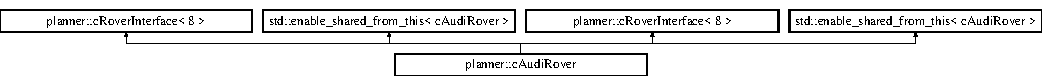
\includegraphics[height=2.000000cm]{classplanner_1_1c_audi_rover}
\end{center}
\end{figure}
\subsection*{Public Member Functions}
\begin{DoxyCompactItemize}
\item 
\mbox{\hyperlink{classplanner_1_1c_audi_rover_a433acb819672e065324dbbdb2a077ecb}{c\+Audi\+Rover}} (uint8\+\_\+t $\ast$i\+\_\+po\+Elevation, uint8\+\_\+t $\ast$i\+\_\+po\+Overrides, uint32\+\_\+t i\+\_\+n\+Height, uint32\+\_\+t i\+\_\+n\+Width)
\item 
\mbox{\Hypertarget{classplanner_1_1c_audi_rover_a52c48afa0829f858c19d3ecf4940db21}\label{classplanner_1_1c_audi_rover_a52c48afa0829f858c19d3ecf4940db21}} 
void \mbox{\hyperlink{classplanner_1_1c_audi_rover_a52c48afa0829f858c19d3ecf4940db21}{Summon}} (uint8\+\_\+t i\+\_\+n\+Step\+Size=1, uint8\+\_\+t i\+\_\+n\+Velocity=1)
\begin{DoxyCompactList}\small\item\em The summon feature that the Audi rover provides. \end{DoxyCompactList}\item 
\mbox{\Hypertarget{classplanner_1_1c_audi_rover_a7a463160a532a99e06a98fce3df4d2c3}\label{classplanner_1_1c_audi_rover_a7a463160a532a99e06a98fce3df4d2c3}} 
void {\bfseries Initialize\+Planner} (const uint8\+\_\+t \&i\+\_\+n\+Step\+Size, const uint8\+\_\+t \&i\+\_\+n\+Velocity) override
\end{DoxyCompactItemize}
\subsection*{Additional Inherited Members}


\subsection{Constructor \& Destructor Documentation}
\mbox{\Hypertarget{classplanner_1_1c_audi_rover_a433acb819672e065324dbbdb2a077ecb}\label{classplanner_1_1c_audi_rover_a433acb819672e065324dbbdb2a077ecb}} 
\index{planner\+::c\+Audi\+Rover@{planner\+::c\+Audi\+Rover}!c\+Audi\+Rover@{c\+Audi\+Rover}}
\index{c\+Audi\+Rover@{c\+Audi\+Rover}!planner\+::c\+Audi\+Rover@{planner\+::c\+Audi\+Rover}}
\subsubsection{\texorpdfstring{c\+Audi\+Rover()}{cAudiRover()}}
{\footnotesize\ttfamily planner\+::c\+Audi\+Rover\+::c\+Audi\+Rover (\begin{DoxyParamCaption}\item[{uint8\+\_\+t $\ast$}]{i\+\_\+po\+Elevation,  }\item[{uint8\+\_\+t $\ast$}]{i\+\_\+po\+Overrides,  }\item[{uint32\+\_\+t}]{i\+\_\+n\+Height,  }\item[{uint32\+\_\+t}]{i\+\_\+n\+Width }\end{DoxyParamCaption})}

Define direction and cost of different possible actions 

The documentation for this class was generated from the following files\+:\begin{DoxyCompactItemize}
\item 
/\+Users/fjp/git/bachelor/planner/include/audi\+\_\+rover.\+h\item 
/\+Users/fjp/git/bachelor/planner/src/audi\+\_\+rover.\+cpp\end{DoxyCompactItemize}

\hypertarget{classplanner_1_1c_graph}{}\section{planner\+:\+:c\+Graph Class Reference}
\label{classplanner_1_1c_graph}\index{planner\+::c\+Graph@{planner\+::c\+Graph}}


The map class c\+Map has pointers to the elevation.\+data (m\+\_\+po\+Elevation) and overrides.\+data (m\+\_\+po\+Overrides).  




{\ttfamily \#include $<$graph.\+h$>$}

\subsection*{Public Member Functions}
\begin{DoxyCompactItemize}
\item 
\mbox{\Hypertarget{classplanner_1_1c_graph_a189aeb64fe91fd6dd07f4b068d3b791e}\label{classplanner_1_1c_graph_a189aeb64fe91fd6dd07f4b068d3b791e}} 
\mbox{\hyperlink{classplanner_1_1c_graph_a189aeb64fe91fd6dd07f4b068d3b791e}{c\+Graph}} (uint8\+\_\+t $\ast$i\+\_\+o\+Elevation, uint8\+\_\+t $\ast$i\+\_\+o\+Overrides, int i\+\_\+n\+Height, int i\+\_\+n\+Width)
\begin{DoxyCompactList}\small\item\em Initializes the members m\+\_\+po\+Elevation, m\+\_\+po\+Overrides and the maps height m\+\_\+n\+Height and width m\+\_\+n\+Width. \end{DoxyCompactList}\item 
uint8\+\_\+t \mbox{\hyperlink{classplanner_1_1c_graph_a0e01eaa240f5e4f5020df2d611ab1994}{Elevation}} (int i\+\_\+nX, int i\+\_\+nY)
\begin{DoxyCompactList}\small\item\em Get elevation at provided location. \end{DoxyCompactList}\item 
\mbox{\Hypertarget{classplanner_1_1c_graph_adf0a3350d15819b92ec14c4596ebf702}\label{classplanner_1_1c_graph_adf0a3350d15819b92ec14c4596ebf702}} 
uint8\+\_\+t {\bfseries Overrides} (int i\+\_\+nX, int i\+\_\+nY)
\item 
bool \mbox{\hyperlink{classplanner_1_1c_graph_a97108b0e05fa547c006d76e749d52f27}{Water}} (int i\+\_\+nX, int i\+\_\+nY)
\begin{DoxyCompactList}\small\item\em Check if the position is on mainland or water. \end{DoxyCompactList}\item 
bool \mbox{\hyperlink{classplanner_1_1c_graph_a99935ff4c32d229e6006aaa843a685a9}{Water}} (int i\+\_\+n\+X0, int i\+\_\+n\+Y0, int i\+\_\+n\+X1, int i\+\_\+n\+Y1)
\begin{DoxyCompactList}\small\item\em Check if the position between the two locations is on mainland or water or goes through it. \end{DoxyCompactList}\item 
int \mbox{\hyperlink{classplanner_1_1c_graph_a5c163af76e19303794a908304f3b759e}{Height}} () const
\begin{DoxyCompactList}\small\item\em Getter for the height of the map, stored in m\+\_\+n\+Height. \end{DoxyCompactList}\item 
int \mbox{\hyperlink{classplanner_1_1c_graph_a25e3f4ee33c86a8a0c3a31c42dac7607}{Width}} () const
\begin{DoxyCompactList}\small\item\em Getter for the width of the map, stored in m\+\_\+n\+Width. \end{DoxyCompactList}\item 
void \mbox{\hyperlink{classplanner_1_1c_graph_a6da6e6e269013628aef48245a7787cb9}{Set\+Overrides}} (int i\+\_\+nX, int i\+\_\+nY, uint8\+\_\+t i\+\_\+n\+Value)
\begin{DoxyCompactList}\small\item\em Sets the provided overrides m\+\_\+po\+Overrides 8 bit value i\+\_\+n\+Value at the provided location while keeping the old value (or operation). \end{DoxyCompactList}\end{DoxyCompactItemize}
\subsection*{Public Attributes}
\begin{DoxyCompactItemize}
\item 
\mbox{\Hypertarget{classplanner_1_1c_graph_aea1ab1d83e0e58f454f07a46fc0d40dd}\label{classplanner_1_1c_graph_aea1ab1d83e0e58f454f07a46fc0d40dd}} 
uint8\+\_\+t $\ast$ \mbox{\hyperlink{classplanner_1_1c_graph_aea1ab1d83e0e58f454f07a46fc0d40dd}{m\+\_\+o\+Elevation}}
\begin{DoxyCompactList}\small\item\em Elevation over the ground (0-\/255). \end{DoxyCompactList}\item 
\mbox{\Hypertarget{classplanner_1_1c_graph_a0794d9865c56cddd3d051e6ea0c1c756}\label{classplanner_1_1c_graph_a0794d9865c56cddd3d051e6ea0c1c756}} 
uint8\+\_\+t $\ast$ {\bfseries m\+\_\+o\+Overrides}
\item 
\mbox{\Hypertarget{classplanner_1_1c_graph_a5bb5ea1aa1709b4530bbf5f931c1f277}\label{classplanner_1_1c_graph_a5bb5ea1aa1709b4530bbf5f931c1f277}} 
int \mbox{\hyperlink{classplanner_1_1c_graph_a5bb5ea1aa1709b4530bbf5f931c1f277}{m\+\_\+n\+Height}}
\begin{DoxyCompactList}\small\item\em Stores the height of the map. \end{DoxyCompactList}\item 
\mbox{\Hypertarget{classplanner_1_1c_graph_a91f89c2fde0344dc74060297b2d5235e}\label{classplanner_1_1c_graph_a91f89c2fde0344dc74060297b2d5235e}} 
int \mbox{\hyperlink{classplanner_1_1c_graph_a91f89c2fde0344dc74060297b2d5235e}{m\+\_\+n\+Width}}
\begin{DoxyCompactList}\small\item\em Stores the width of the map. \end{DoxyCompactList}\end{DoxyCompactItemize}


\subsection{Detailed Description}
The map class c\+Map has pointers to the elevation.\+data (m\+\_\+po\+Elevation) and overrides.\+data (m\+\_\+po\+Overrides). 

This class is used to check for constraints in the map (e.\+g. water basins, rivers and marsh, which cannot be traversed by the robot. The elevation data is used to model the acceleration of the rover. 

\subsection{Member Function Documentation}
\mbox{\Hypertarget{classplanner_1_1c_graph_a0e01eaa240f5e4f5020df2d611ab1994}\label{classplanner_1_1c_graph_a0e01eaa240f5e4f5020df2d611ab1994}} 
\index{planner\+::c\+Graph@{planner\+::c\+Graph}!Elevation@{Elevation}}
\index{Elevation@{Elevation}!planner\+::c\+Graph@{planner\+::c\+Graph}}
\subsubsection{\texorpdfstring{Elevation()}{Elevation()}}
{\footnotesize\ttfamily uint8\+\_\+t planner\+::c\+Graph\+::\+Elevation (\begin{DoxyParamCaption}\item[{int}]{i\+\_\+nX,  }\item[{int}]{i\+\_\+nY }\end{DoxyParamCaption})}



Get elevation at provided location. 

From the read elevation.\+data the 8 bit value is returned. 
\begin{DoxyParams}[1]{Parameters}
\mbox{\tt in}  & {\em i\+\_\+nX} & X location of the elevation. \\
\hline
\mbox{\tt in}  & {\em i\+\_\+nY} & Y location of the elevation. \\
\hline
\end{DoxyParams}
\begin{DoxyReturn}{Returns}
Elevation at (i\+\_\+nX, i\+\_\+nY). 
\end{DoxyReturn}
\mbox{\Hypertarget{classplanner_1_1c_graph_a5c163af76e19303794a908304f3b759e}\label{classplanner_1_1c_graph_a5c163af76e19303794a908304f3b759e}} 
\index{planner\+::c\+Graph@{planner\+::c\+Graph}!Height@{Height}}
\index{Height@{Height}!planner\+::c\+Graph@{planner\+::c\+Graph}}
\subsubsection{\texorpdfstring{Height()}{Height()}}
{\footnotesize\ttfamily int planner\+::c\+Graph\+::\+Height (\begin{DoxyParamCaption}{ }\end{DoxyParamCaption}) const}



Getter for the height of the map, stored in m\+\_\+n\+Height. 

\begin{DoxyReturn}{Returns}
The total height of the map. 
\end{DoxyReturn}
\mbox{\Hypertarget{classplanner_1_1c_graph_a6da6e6e269013628aef48245a7787cb9}\label{classplanner_1_1c_graph_a6da6e6e269013628aef48245a7787cb9}} 
\index{planner\+::c\+Graph@{planner\+::c\+Graph}!Set\+Overrides@{Set\+Overrides}}
\index{Set\+Overrides@{Set\+Overrides}!planner\+::c\+Graph@{planner\+::c\+Graph}}
\subsubsection{\texorpdfstring{Set\+Overrides()}{SetOverrides()}}
{\footnotesize\ttfamily void planner\+::c\+Graph\+::\+Set\+Overrides (\begin{DoxyParamCaption}\item[{int}]{i\+\_\+nX,  }\item[{int}]{i\+\_\+nY,  }\item[{uint8\+\_\+t}]{i\+\_\+n\+Value }\end{DoxyParamCaption})}



Sets the provided overrides m\+\_\+po\+Overrides 8 bit value i\+\_\+n\+Value at the provided location while keeping the old value (or operation). 


\begin{DoxyParams}[1]{Parameters}
\mbox{\tt in}  & {\em i\+\_\+nX} & X location of the overrides m\+\_\+po\+Overrides that should be updated. \\
\hline
\mbox{\tt in}  & {\em i\+\_\+nY} & Y location of the overrides m\+\_\+po\+Overrides that should be updated. \\
\hline
\mbox{\tt in}  & {\em i\+\_\+n\+Value} & The or operator is applied to this 8 bit mask value and the current overrides value at (i\+\_\+nX, i\+\_\+nY). \\
\hline
\end{DoxyParams}
\mbox{\Hypertarget{classplanner_1_1c_graph_a97108b0e05fa547c006d76e749d52f27}\label{classplanner_1_1c_graph_a97108b0e05fa547c006d76e749d52f27}} 
\index{planner\+::c\+Graph@{planner\+::c\+Graph}!Water@{Water}}
\index{Water@{Water}!planner\+::c\+Graph@{planner\+::c\+Graph}}
\subsubsection{\texorpdfstring{Water()}{Water()}\hspace{0.1cm}{\footnotesize\ttfamily [1/2]}}
{\footnotesize\ttfamily bool planner\+::c\+Graph\+::\+Water (\begin{DoxyParamCaption}\item[{int}]{i\+\_\+nX,  }\item[{int}]{i\+\_\+nY }\end{DoxyParamCaption})}



Check if the position is on mainland or water. 


\begin{DoxyParams}[1]{Parameters}
\mbox{\tt in}  & {\em i\+\_\+nX} & X coordinate to be checked for water. \\
\hline
\mbox{\tt in}  & {\em i\+\_\+nY} & Y coordinate to be checked for water. \\
\hline
\end{DoxyParams}
\begin{DoxyReturn}{Returns}
true if the provided position is on water, false otherwise. 
\end{DoxyReturn}
\mbox{\Hypertarget{classplanner_1_1c_graph_a99935ff4c32d229e6006aaa843a685a9}\label{classplanner_1_1c_graph_a99935ff4c32d229e6006aaa843a685a9}} 
\index{planner\+::c\+Graph@{planner\+::c\+Graph}!Water@{Water}}
\index{Water@{Water}!planner\+::c\+Graph@{planner\+::c\+Graph}}
\subsubsection{\texorpdfstring{Water()}{Water()}\hspace{0.1cm}{\footnotesize\ttfamily [2/2]}}
{\footnotesize\ttfamily bool planner\+::c\+Graph\+::\+Water (\begin{DoxyParamCaption}\item[{int}]{i\+\_\+n\+X0,  }\item[{int}]{i\+\_\+n\+Y0,  }\item[{int}]{i\+\_\+n\+X1,  }\item[{int}]{i\+\_\+n\+Y1 }\end{DoxyParamCaption})}



Check if the position between the two locations is on mainland or water or goes through it. 


\begin{DoxyParams}[1]{Parameters}
\mbox{\tt in}  & {\em i\+\_\+nX} & X coordinate to be checked for water. \\
\hline
\mbox{\tt in}  & {\em i\+\_\+nY} & Y coordinate to be checked for water. \\
\hline
\end{DoxyParams}
\begin{DoxyReturn}{Returns}
true if the provided position is on or goes through water, false otherwise. 
\end{DoxyReturn}
\mbox{\Hypertarget{classplanner_1_1c_graph_a25e3f4ee33c86a8a0c3a31c42dac7607}\label{classplanner_1_1c_graph_a25e3f4ee33c86a8a0c3a31c42dac7607}} 
\index{planner\+::c\+Graph@{planner\+::c\+Graph}!Width@{Width}}
\index{Width@{Width}!planner\+::c\+Graph@{planner\+::c\+Graph}}
\subsubsection{\texorpdfstring{Width()}{Width()}}
{\footnotesize\ttfamily int planner\+::c\+Graph\+::\+Width (\begin{DoxyParamCaption}{ }\end{DoxyParamCaption}) const}



Getter for the width of the map, stored in m\+\_\+n\+Width. 

\begin{DoxyReturn}{Returns}
The total width of the map. 
\end{DoxyReturn}


The documentation for this class was generated from the following files\+:\begin{DoxyCompactItemize}
\item 
/\+Users/fjp/git/bachelor/planner/include/graph.\+h\item 
/\+Users/fjp/git/bachelor/planner/src/graph.\+cpp\end{DoxyCompactItemize}

\hypertarget{classupload_1_1_client_login_error}{}\section{upload.\+Client\+Login\+Error Class Reference}
\label{classupload_1_1_client_login_error}\index{upload.\+Client\+Login\+Error@{upload.\+Client\+Login\+Error}}
Inheritance diagram for upload.\+Client\+Login\+Error\+:\begin{figure}[H]
\begin{center}
\leavevmode
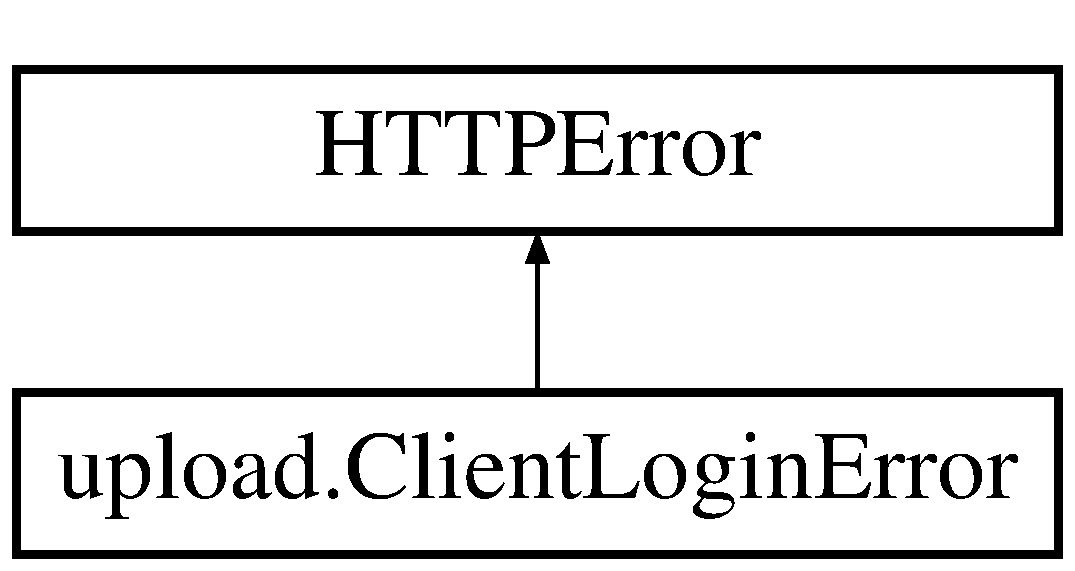
\includegraphics[height=2.000000cm]{classupload_1_1_client_login_error}
\end{center}
\end{figure}
\subsection*{Public Member Functions}
\begin{DoxyCompactItemize}
\item 
\mbox{\Hypertarget{classupload_1_1_client_login_error_a1e590616c2976d881e155958cedbbe47}\label{classupload_1_1_client_login_error_a1e590616c2976d881e155958cedbbe47}} 
def {\bfseries \+\_\+\+\_\+init\+\_\+\+\_\+} (self, url, code, msg, headers, args)
\end{DoxyCompactItemize}
\subsection*{Public Attributes}
\begin{DoxyCompactItemize}
\item 
\mbox{\Hypertarget{classupload_1_1_client_login_error_ac300a0b034b2bc64cedc51e09fb6d663}\label{classupload_1_1_client_login_error_ac300a0b034b2bc64cedc51e09fb6d663}} 
{\bfseries args}
\item 
\mbox{\Hypertarget{classupload_1_1_client_login_error_ae0555feb182d89d1e4d7944afbfe14e5}\label{classupload_1_1_client_login_error_ae0555feb182d89d1e4d7944afbfe14e5}} 
{\bfseries reason}
\end{DoxyCompactItemize}


\subsection{Detailed Description}
\begin{DoxyVerb}Raised to indicate there was an error authenticating with ClientLogin.\end{DoxyVerb}
 

The documentation for this class was generated from the following file\+:\begin{DoxyCompactItemize}
\item 
/\+Users/fjp/git/bachelor/bachelor-\/master\+\_\+updated\+\_\+vfinal/googletest-\/1.\+8.\+0/googletest/scripts/upload.\+py\end{DoxyCompactItemize}

\hypertarget{structtesting_1_1internal_1_1_code_location}{}\section{testing\+:\+:internal\+:\+:Code\+Location Struct Reference}
\label{structtesting_1_1internal_1_1_code_location}\index{testing\+::internal\+::\+Code\+Location@{testing\+::internal\+::\+Code\+Location}}
\subsection*{Public Member Functions}
\begin{DoxyCompactItemize}
\item 
\mbox{\Hypertarget{structtesting_1_1internal_1_1_code_location_ade3ecb2a54905619cd40a6856b48cd5a}\label{structtesting_1_1internal_1_1_code_location_ade3ecb2a54905619cd40a6856b48cd5a}} 
{\bfseries Code\+Location} (const string \&a\+\_\+file, int a\+\_\+line)
\end{DoxyCompactItemize}
\subsection*{Public Attributes}
\begin{DoxyCompactItemize}
\item 
\mbox{\Hypertarget{structtesting_1_1internal_1_1_code_location_ab8a24d5e63295e411d37578dbb9427c0}\label{structtesting_1_1internal_1_1_code_location_ab8a24d5e63295e411d37578dbb9427c0}} 
string {\bfseries file}
\item 
\mbox{\Hypertarget{structtesting_1_1internal_1_1_code_location_a01c977c7e8834a05a6d6c40b0c416045}\label{structtesting_1_1internal_1_1_code_location_a01c977c7e8834a05a6d6c40b0c416045}} 
int {\bfseries line}
\end{DoxyCompactItemize}


The documentation for this struct was generated from the following file\+:\begin{DoxyCompactItemize}
\item 
/\+Users/fjp/git/bachelor/bachelor-\/master\+\_\+updated\+\_\+vfinal/googletest-\/1.\+8.\+0/googletest/include/gtest/internal/gtest-\/internal.\+h\end{DoxyCompactItemize}

\hypertarget{classtesting_1_1_code_location_for_t_e_s_t_f}{}\section{testing\+:\+:Code\+Location\+For\+T\+E\+S\+TF Class Reference}
\label{classtesting_1_1_code_location_for_t_e_s_t_f}\index{testing\+::\+Code\+Location\+For\+T\+E\+S\+TF@{testing\+::\+Code\+Location\+For\+T\+E\+S\+TF}}
Inheritance diagram for testing\+:\+:Code\+Location\+For\+T\+E\+S\+TF\+:\begin{figure}[H]
\begin{center}
\leavevmode
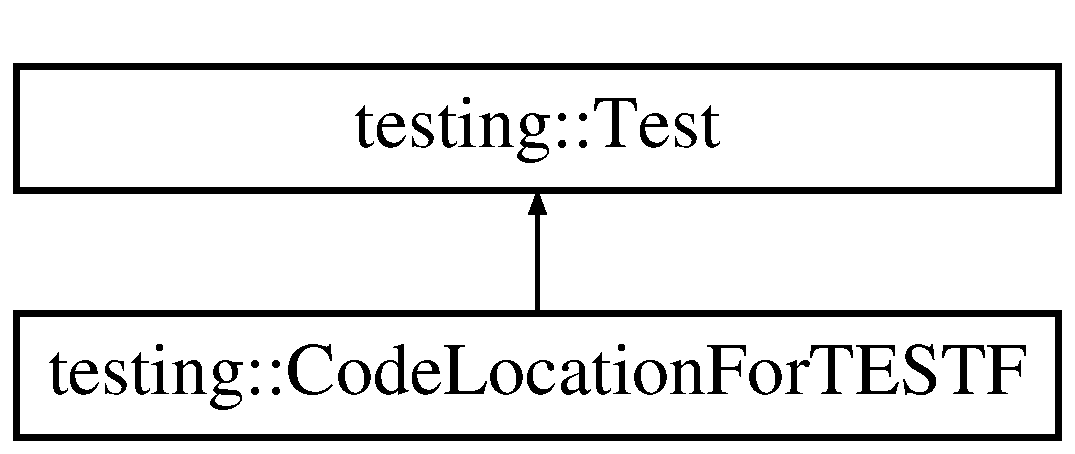
\includegraphics[height=2.000000cm]{classtesting_1_1_code_location_for_t_e_s_t_f}
\end{center}
\end{figure}
\subsection*{Additional Inherited Members}


The documentation for this class was generated from the following file\+:\begin{DoxyCompactItemize}
\item 
/\+Users/fjp/git/bachelor/bachelor-\/master\+\_\+updated\+\_\+vfinal/googletest-\/1.\+8.\+0/googletest/test/gtest\+\_\+unittest.\+cc\end{DoxyCompactItemize}

\hypertarget{classtesting_1_1_code_location_for_t_e_s_t_p}{}\section{testing\+:\+:Code\+Location\+For\+T\+E\+S\+TP Class Reference}
\label{classtesting_1_1_code_location_for_t_e_s_t_p}\index{testing\+::\+Code\+Location\+For\+T\+E\+S\+TP@{testing\+::\+Code\+Location\+For\+T\+E\+S\+TP}}
Inheritance diagram for testing\+:\+:Code\+Location\+For\+T\+E\+S\+TP\+:\begin{figure}[H]
\begin{center}
\leavevmode
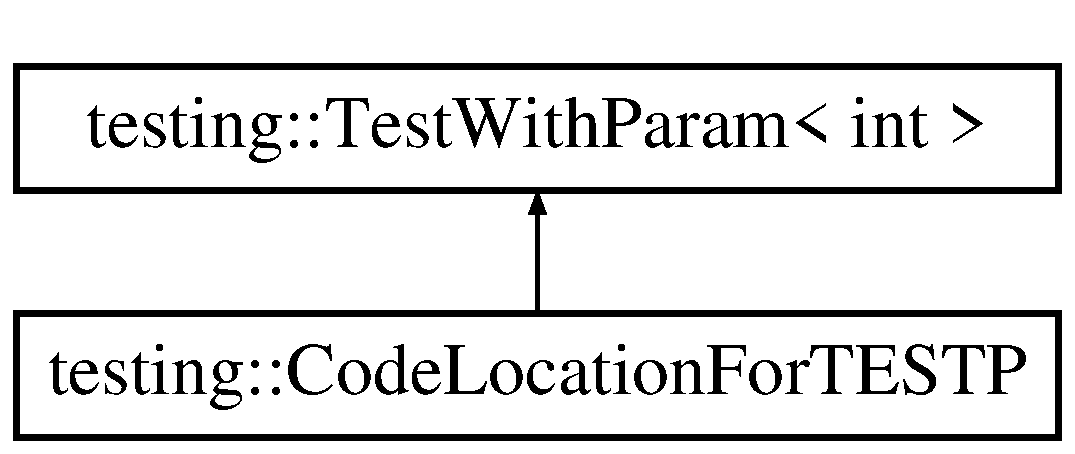
\includegraphics[height=2.000000cm]{classtesting_1_1_code_location_for_t_e_s_t_p}
\end{center}
\end{figure}


The documentation for this class was generated from the following file\+:\begin{DoxyCompactItemize}
\item 
/\+Users/fjp/git/bachelor/bachelor-\/master\+\_\+updated\+\_\+vfinal/googletest-\/1.\+8.\+0/googletest/test/gtest\+\_\+unittest.\+cc\end{DoxyCompactItemize}

\hypertarget{classtesting_1_1_code_location_for_t_y_p_e_d_t_e_s_t}{}\section{testing\+:\+:Code\+Location\+For\+T\+Y\+P\+E\+D\+T\+E\+ST$<$ T $>$ Class Template Reference}
\label{classtesting_1_1_code_location_for_t_y_p_e_d_t_e_s_t}\index{testing\+::\+Code\+Location\+For\+T\+Y\+P\+E\+D\+T\+E\+S\+T$<$ T $>$@{testing\+::\+Code\+Location\+For\+T\+Y\+P\+E\+D\+T\+E\+S\+T$<$ T $>$}}
Inheritance diagram for testing\+:\+:Code\+Location\+For\+T\+Y\+P\+E\+D\+T\+E\+ST$<$ T $>$\+:\begin{figure}[H]
\begin{center}
\leavevmode
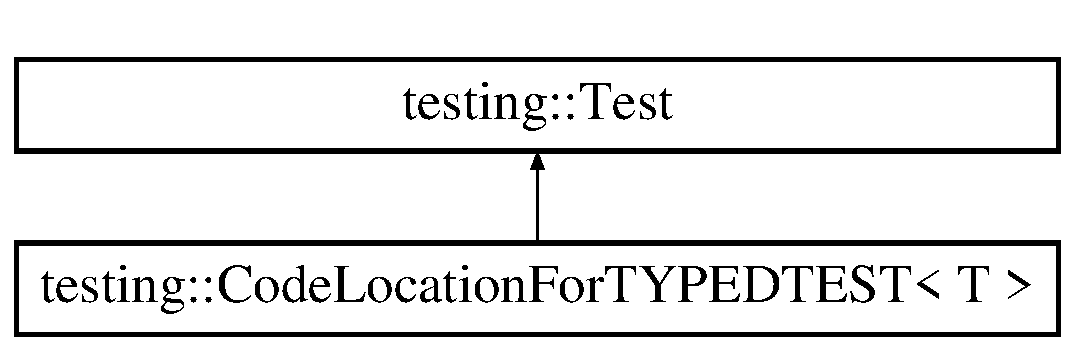
\includegraphics[height=2.000000cm]{classtesting_1_1_code_location_for_t_y_p_e_d_t_e_s_t}
\end{center}
\end{figure}
\subsection*{Additional Inherited Members}


The documentation for this class was generated from the following file\+:\begin{DoxyCompactItemize}
\item 
/\+Users/fjp/git/bachelor/bachelor-\/master\+\_\+updated\+\_\+vfinal/googletest-\/1.\+8.\+0/googletest/test/gtest\+\_\+unittest.\+cc\end{DoxyCompactItemize}

\hypertarget{classtesting_1_1_code_location_for_t_y_p_e_d_t_e_s_t_p}{}\section{testing\+:\+:Code\+Location\+For\+T\+Y\+P\+E\+D\+T\+E\+S\+TP$<$ T $>$ Class Template Reference}
\label{classtesting_1_1_code_location_for_t_y_p_e_d_t_e_s_t_p}\index{testing\+::\+Code\+Location\+For\+T\+Y\+P\+E\+D\+T\+E\+S\+T\+P$<$ T $>$@{testing\+::\+Code\+Location\+For\+T\+Y\+P\+E\+D\+T\+E\+S\+T\+P$<$ T $>$}}
Inheritance diagram for testing\+:\+:Code\+Location\+For\+T\+Y\+P\+E\+D\+T\+E\+S\+TP$<$ T $>$\+:\begin{figure}[H]
\begin{center}
\leavevmode
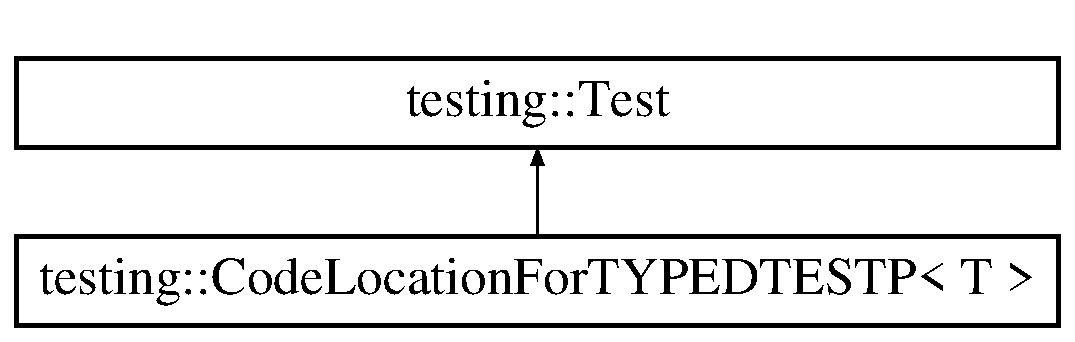
\includegraphics[height=2.000000cm]{classtesting_1_1_code_location_for_t_y_p_e_d_t_e_s_t_p}
\end{center}
\end{figure}
\subsection*{Additional Inherited Members}


The documentation for this class was generated from the following file\+:\begin{DoxyCompactItemize}
\item 
/\+Users/fjp/git/bachelor/bachelor-\/master\+\_\+updated\+\_\+vfinal/googletest-\/1.\+8.\+0/googletest/test/gtest\+\_\+unittest.\+cc\end{DoxyCompactItemize}

\hypertarget{classpump_1_1_code_node}{}\section{pump.\+Code\+Node Class Reference}
\label{classpump_1_1_code_node}\index{pump.\+Code\+Node@{pump.\+Code\+Node}}
\subsection*{Public Member Functions}
\begin{DoxyCompactItemize}
\item 
\mbox{\Hypertarget{classpump_1_1_code_node_a2ca8a75324a64e48004812d6c0bc1cbd}\label{classpump_1_1_code_node_a2ca8a75324a64e48004812d6c0bc1cbd}} 
def {\bfseries \+\_\+\+\_\+init\+\_\+\+\_\+} (self, atomic\+\_\+code\+\_\+list=None)
\end{DoxyCompactItemize}
\subsection*{Public Attributes}
\begin{DoxyCompactItemize}
\item 
\mbox{\Hypertarget{classpump_1_1_code_node_ac7251110cc987c709e0e17d95521993e}\label{classpump_1_1_code_node_ac7251110cc987c709e0e17d95521993e}} 
{\bfseries atomic\+\_\+code}
\end{DoxyCompactItemize}


The documentation for this class was generated from the following file\+:\begin{DoxyCompactItemize}
\item 
/\+Users/fjp/git/bachelor/bachelor-\/master\+\_\+updated\+\_\+vfinal/googletest-\/1.\+8.\+0/googletest/scripts/pump.\+py\end{DoxyCompactItemize}

\hypertarget{class_common_test}{}\section{Common\+Test$<$ T $>$ Class Template Reference}
\label{class_common_test}\index{Common\+Test$<$ T $>$@{Common\+Test$<$ T $>$}}
Inheritance diagram for Common\+Test$<$ T $>$\+:\begin{figure}[H]
\begin{center}
\leavevmode
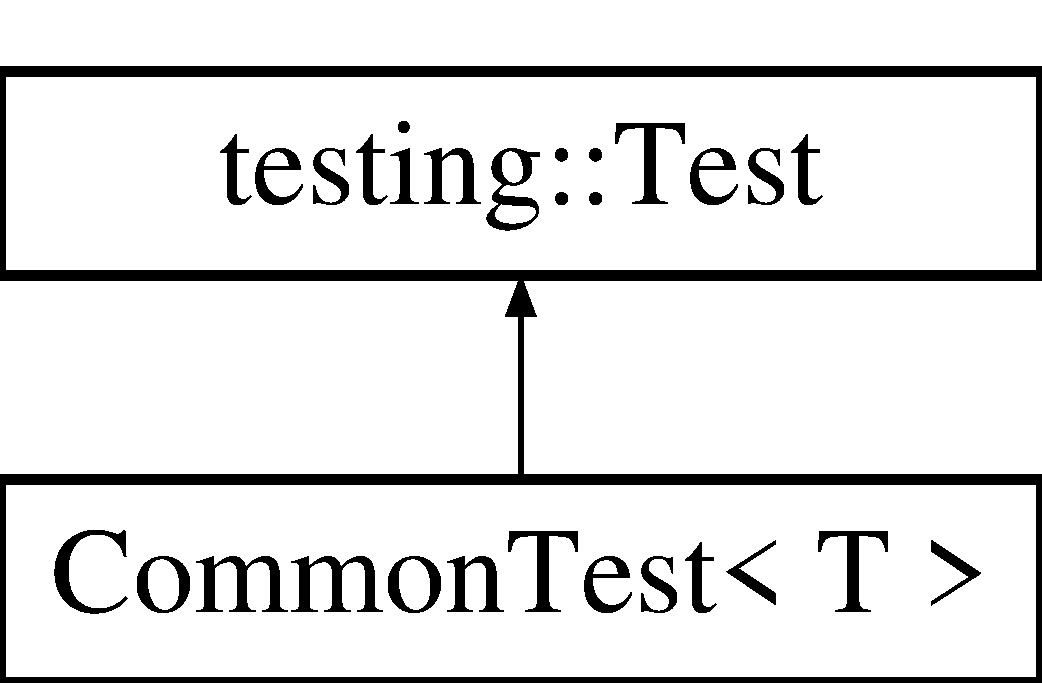
\includegraphics[height=2.000000cm]{class_common_test}
\end{center}
\end{figure}
\subsection*{Static Public Member Functions}
\begin{DoxyCompactItemize}
\item 
\mbox{\Hypertarget{class_common_test_a6edd90f32f45cc49e4a423b22bd770ce}\label{class_common_test_a6edd90f32f45cc49e4a423b22bd770ce}} 
static void {\bfseries Set\+Up\+Test\+Case} ()
\item 
\mbox{\Hypertarget{class_common_test_a68d2bf5108cf28478331588fbdff4838}\label{class_common_test_a68d2bf5108cf28478331588fbdff4838}} 
static void {\bfseries Tear\+Down\+Test\+Case} ()
\end{DoxyCompactItemize}
\subsection*{Protected Types}
\begin{DoxyCompactItemize}
\item 
\mbox{\Hypertarget{class_common_test_a6dfdcede6964887b9f4254a0e0478e37}\label{class_common_test_a6dfdcede6964887b9f4254a0e0478e37}} 
typedef std\+::vector$<$ T $>$ {\bfseries Vector}
\item 
\mbox{\Hypertarget{class_common_test_a62827e9d3064cddf4a8698747f1bd434}\label{class_common_test_a62827e9d3064cddf4a8698747f1bd434}} 
typedef std\+::set$<$ int $>$ {\bfseries Int\+Set}
\end{DoxyCompactItemize}
\subsection*{Protected Member Functions}
\begin{DoxyCompactItemize}
\item 
\mbox{\Hypertarget{class_common_test_a4c7bf7889ce48a9d06530bc4a437f3f5}\label{class_common_test_a4c7bf7889ce48a9d06530bc4a437f3f5}} 
virtual void {\bfseries Set\+Up} ()
\item 
\mbox{\Hypertarget{class_common_test_aeae195c2cefa956c6ae5be1226e6ecd8}\label{class_common_test_aeae195c2cefa956c6ae5be1226e6ecd8}} 
virtual void {\bfseries Tear\+Down} ()
\end{DoxyCompactItemize}
\subsection*{Protected Attributes}
\begin{DoxyCompactItemize}
\item 
\mbox{\Hypertarget{class_common_test_ae59c4abcb833625a7baeb2048531ebec}\label{class_common_test_ae59c4abcb833625a7baeb2048531ebec}} 
T {\bfseries value\+\_\+}
\end{DoxyCompactItemize}
\subsection*{Static Protected Attributes}
\begin{DoxyCompactItemize}
\item 
\mbox{\Hypertarget{class_common_test_a52368ce1e65a865db9bdccbcc2cedaac}\label{class_common_test_a52368ce1e65a865db9bdccbcc2cedaac}} 
static T $\ast$ {\bfseries shared\+\_\+} = N\+U\+LL
\end{DoxyCompactItemize}
\subsection*{Additional Inherited Members}


The documentation for this class was generated from the following file\+:\begin{DoxyCompactItemize}
\item 
/\+Users/fjp/git/bachelor/bachelor-\/master\+\_\+updated\+\_\+vfinal/googletest-\/1.\+8.\+0/googletest/test/gtest-\/typed-\/test\+\_\+test.\+cc\end{DoxyCompactItemize}

\hypertarget{structtesting_1_1internal_1_1_compile_assert}{}\section{testing\+:\+:internal\+:\+:Compile\+Assert$<$ bool $>$ Struct Template Reference}
\label{structtesting_1_1internal_1_1_compile_assert}\index{testing\+::internal\+::\+Compile\+Assert$<$ bool $>$@{testing\+::internal\+::\+Compile\+Assert$<$ bool $>$}}


The documentation for this struct was generated from the following file\+:\begin{DoxyCompactItemize}
\item 
/\+Users/fjp/git/bachelor/bachelor-\/master\+\_\+updated\+\_\+vfinal/googletest-\/1.\+8.\+0/googletest/include/gtest/internal/gtest-\/port.\+h\end{DoxyCompactItemize}

\hypertarget{structtesting_1_1internal_1_1_compile_assert_types_equal}{}\section{testing\+:\+:internal\+:\+:Compile\+Assert\+Types\+Equal$<$ T1, T2 $>$ Struct Template Reference}
\label{structtesting_1_1internal_1_1_compile_assert_types_equal}\index{testing\+::internal\+::\+Compile\+Assert\+Types\+Equal$<$ T1, T2 $>$@{testing\+::internal\+::\+Compile\+Assert\+Types\+Equal$<$ T1, T2 $>$}}


The documentation for this struct was generated from the following file\+:\begin{DoxyCompactItemize}
\item 
/\+Users/fjp/git/bachelor/bachelor-\/master\+\_\+updated\+\_\+vfinal/googletest-\/1.\+8.\+0/googletest/include/gtest/internal/gtest-\/internal.\+h\end{DoxyCompactItemize}

\hypertarget{structtesting_1_1internal_1_1_compile_assert_types_equal_3_01_t_00_01_t_01_4}{}\section{testing\+:\+:internal\+:\+:Compile\+Assert\+Types\+Equal$<$ T, T $>$ Struct Template Reference}
\label{structtesting_1_1internal_1_1_compile_assert_types_equal_3_01_t_00_01_t_01_4}\index{testing\+::internal\+::\+Compile\+Assert\+Types\+Equal$<$ T, T $>$@{testing\+::internal\+::\+Compile\+Assert\+Types\+Equal$<$ T, T $>$}}


The documentation for this struct was generated from the following file\+:\begin{DoxyCompactItemize}
\item 
/\+Users/fjp/git/bachelor/bachelor-\/master\+\_\+updated\+\_\+vfinal/googletest-\/1.\+8.\+0/googletest/include/gtest/internal/gtest-\/internal.\+h\end{DoxyCompactItemize}

\hypertarget{structtesting_1_1gtest__printers__test_1_1const__iterator}{}\section{testing\+:\+:gtest\+\_\+printers\+\_\+test\+:\+:const\+\_\+iterator Struct Reference}
\label{structtesting_1_1gtest__printers__test_1_1const__iterator}\index{testing\+::gtest\+\_\+printers\+\_\+test\+::const\+\_\+iterator@{testing\+::gtest\+\_\+printers\+\_\+test\+::const\+\_\+iterator}}
\subsection*{Public Attributes}
\begin{DoxyCompactItemize}
\item 
\mbox{\Hypertarget{structtesting_1_1gtest__printers__test_1_1const__iterator_a4412dbc1c37c2bc5211971f0c8176d6b}\label{structtesting_1_1gtest__printers__test_1_1const__iterator_a4412dbc1c37c2bc5211971f0c8176d6b}} 
char {\bfseries x}
\end{DoxyCompactItemize}


The documentation for this struct was generated from the following file\+:\begin{DoxyCompactItemize}
\item 
/\+Users/fjp/git/bachelor/bachelor-\/master\+\_\+updated\+\_\+vfinal/googletest-\/1.\+8.\+0/googletest/test/gtest-\/printers\+\_\+test.\+cc\end{DoxyCompactItemize}

\hypertarget{classtesting_1_1internal_1_1_const_and_non_const_castable}{}\section{testing\+:\+:internal\+:\+:Const\+And\+Non\+Const\+Castable Class Reference}
\label{classtesting_1_1internal_1_1_const_and_non_const_castable}\index{testing\+::internal\+::\+Const\+And\+Non\+Const\+Castable@{testing\+::internal\+::\+Const\+And\+Non\+Const\+Castable}}
\subsection*{Public Member Functions}
\begin{DoxyCompactItemize}
\item 
\mbox{\Hypertarget{classtesting_1_1internal_1_1_const_and_non_const_castable_aebe0ef6897b7f805e227bb969d4ee034}\label{classtesting_1_1internal_1_1_const_and_non_const_castable_aebe0ef6897b7f805e227bb969d4ee034}} 
{\bfseries Const\+And\+Non\+Const\+Castable} (bool $\ast$converted, bool $\ast$const\+\_\+converted)
\item 
\mbox{\Hypertarget{classtesting_1_1internal_1_1_const_and_non_const_castable_aff0c372d429d76d002bb29f83f2429fa}\label{classtesting_1_1internal_1_1_const_and_non_const_castable_aff0c372d429d76d002bb29f83f2429fa}} 
{\bfseries operator Base} ()
\item 
\mbox{\Hypertarget{classtesting_1_1internal_1_1_const_and_non_const_castable_a4e8ee8051162f1dfc1da294c71481e2f}\label{classtesting_1_1internal_1_1_const_and_non_const_castable_a4e8ee8051162f1dfc1da294c71481e2f}} 
{\bfseries operator Base} () const
\end{DoxyCompactItemize}


The documentation for this class was generated from the following file\+:\begin{DoxyCompactItemize}
\item 
/\+Users/fjp/git/bachelor/bachelor-\/master\+\_\+updated\+\_\+vfinal/googletest-\/1.\+8.\+0/googletest/test/gtest-\/port\+\_\+test.\+cc\end{DoxyCompactItemize}

\hypertarget{classtesting_1_1internal_1_1_const_castable}{}\section{testing\+:\+:internal\+:\+:Const\+Castable Class Reference}
\label{classtesting_1_1internal_1_1_const_castable}\index{testing\+::internal\+::\+Const\+Castable@{testing\+::internal\+::\+Const\+Castable}}
\subsection*{Public Member Functions}
\begin{DoxyCompactItemize}
\item 
\mbox{\Hypertarget{classtesting_1_1internal_1_1_const_castable_a78eba470cc71528237a33a10a92fba7e}\label{classtesting_1_1internal_1_1_const_castable_a78eba470cc71528237a33a10a92fba7e}} 
{\bfseries Const\+Castable} (bool $\ast$converted)
\item 
\mbox{\Hypertarget{classtesting_1_1internal_1_1_const_castable_af084893d6786010022297b1e88f4743b}\label{classtesting_1_1internal_1_1_const_castable_af084893d6786010022297b1e88f4743b}} 
{\bfseries operator Base} () const
\end{DoxyCompactItemize}


The documentation for this class was generated from the following file\+:\begin{DoxyCompactItemize}
\item 
/\+Users/fjp/git/bachelor/bachelor-\/master\+\_\+updated\+\_\+vfinal/googletest-\/1.\+8.\+0/googletest/test/gtest-\/port\+\_\+test.\+cc\end{DoxyCompactItemize}

\hypertarget{structtesting_1_1internal_1_1_const_char_ptr}{}\section{testing\+:\+:internal\+:\+:Const\+Char\+Ptr Struct Reference}
\label{structtesting_1_1internal_1_1_const_char_ptr}\index{testing\+::internal\+::\+Const\+Char\+Ptr@{testing\+::internal\+::\+Const\+Char\+Ptr}}
\subsection*{Public Member Functions}
\begin{DoxyCompactItemize}
\item 
\mbox{\Hypertarget{structtesting_1_1internal_1_1_const_char_ptr_ae94f6453fa679d815994eccc63062907}\label{structtesting_1_1internal_1_1_const_char_ptr_ae94f6453fa679d815994eccc63062907}} 
{\bfseries Const\+Char\+Ptr} (const char $\ast$str)
\item 
\mbox{\Hypertarget{structtesting_1_1internal_1_1_const_char_ptr_a85c8174b5d4db8fe96863509ba767b27}\label{structtesting_1_1internal_1_1_const_char_ptr_a85c8174b5d4db8fe96863509ba767b27}} 
{\bfseries operator bool} () const
\end{DoxyCompactItemize}
\subsection*{Public Attributes}
\begin{DoxyCompactItemize}
\item 
\mbox{\Hypertarget{structtesting_1_1internal_1_1_const_char_ptr_adba40d23d5986904b605946f643cf26e}\label{structtesting_1_1internal_1_1_const_char_ptr_adba40d23d5986904b605946f643cf26e}} 
const char $\ast$ {\bfseries value}
\end{DoxyCompactItemize}


The documentation for this struct was generated from the following file\+:\begin{DoxyCompactItemize}
\item 
/\+Users/fjp/git/bachelor/bachelor-\/master\+\_\+updated\+\_\+vfinal/googletest-\/1.\+8.\+0/googletest/include/gtest/internal/gtest-\/internal.\+h\end{DoxyCompactItemize}

\hypertarget{class_conversion_helper_base}{}\section{Conversion\+Helper\+Base Class Reference}
\label{class_conversion_helper_base}\index{Conversion\+Helper\+Base@{Conversion\+Helper\+Base}}
Inheritance diagram for Conversion\+Helper\+Base\+:\begin{figure}[H]
\begin{center}
\leavevmode
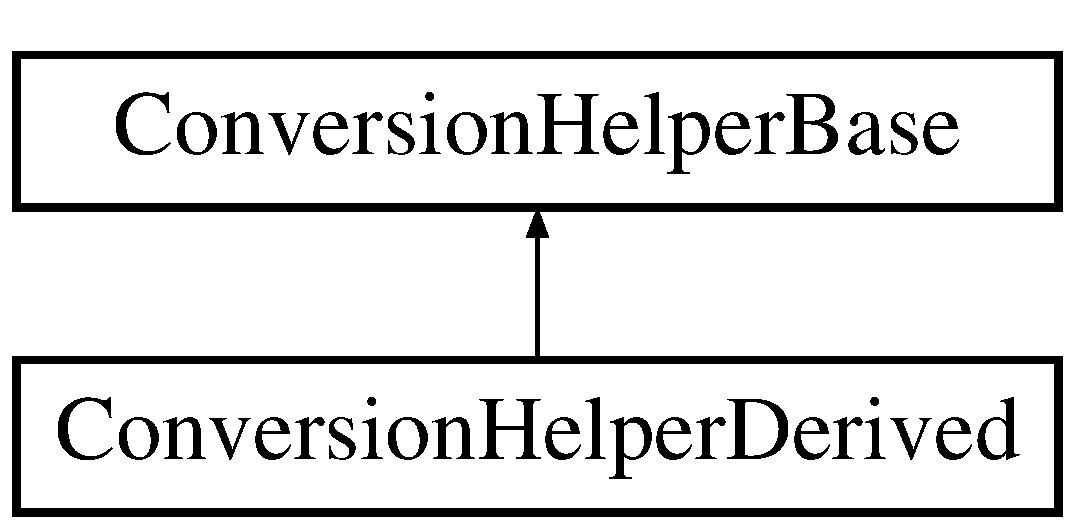
\includegraphics[height=2.000000cm]{class_conversion_helper_base}
\end{center}
\end{figure}


The documentation for this class was generated from the following file\+:\begin{DoxyCompactItemize}
\item 
/\+Users/fjp/git/bachelor/bachelor-\/master\+\_\+updated\+\_\+vfinal/googletest-\/1.\+8.\+0/googletest/test/gtest\+\_\+unittest.\+cc\end{DoxyCompactItemize}

\hypertarget{class_conversion_helper_derived}{}\section{Conversion\+Helper\+Derived Class Reference}
\label{class_conversion_helper_derived}\index{Conversion\+Helper\+Derived@{Conversion\+Helper\+Derived}}
Inheritance diagram for Conversion\+Helper\+Derived\+:\begin{figure}[H]
\begin{center}
\leavevmode
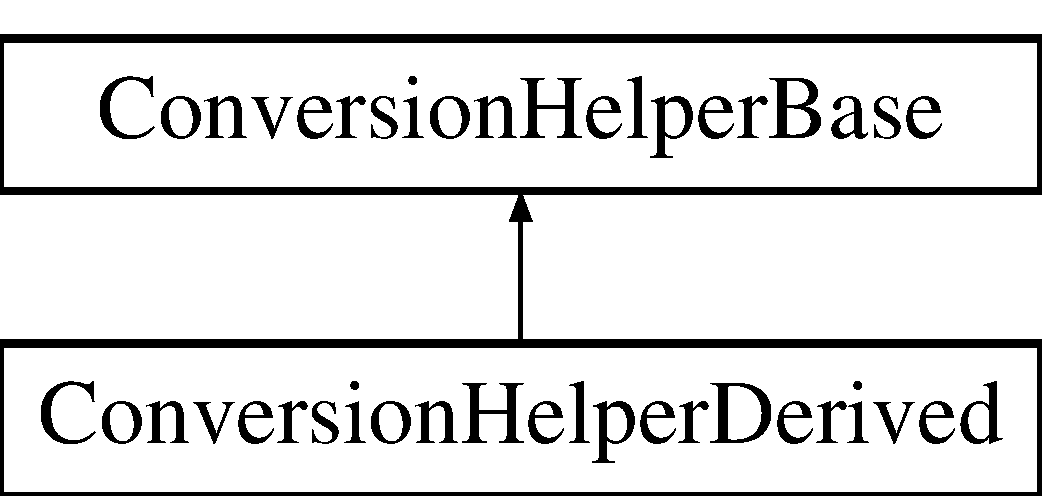
\includegraphics[height=2.000000cm]{class_conversion_helper_derived}
\end{center}
\end{figure}


The documentation for this class was generated from the following file\+:\begin{DoxyCompactItemize}
\item 
/\+Users/fjp/git/bachelor/bachelor-\/master\+\_\+updated\+\_\+vfinal/googletest-\/1.\+8.\+0/googletest/test/gtest\+\_\+unittest.\+cc\end{DoxyCompactItemize}

\hypertarget{struct_convertible_to_assertion_result}{}\section{Convertible\+To\+Assertion\+Result Struct Reference}
\label{struct_convertible_to_assertion_result}\index{Convertible\+To\+Assertion\+Result@{Convertible\+To\+Assertion\+Result}}
\subsection*{Public Member Functions}
\begin{DoxyCompactItemize}
\item 
\mbox{\Hypertarget{struct_convertible_to_assertion_result_a0f816f2f25ecaf29a95b3cfd4033e105}\label{struct_convertible_to_assertion_result_a0f816f2f25ecaf29a95b3cfd4033e105}} 
{\bfseries operator Assertion\+Result} () const
\end{DoxyCompactItemize}


The documentation for this struct was generated from the following file\+:\begin{DoxyCompactItemize}
\item 
/\+Users/fjp/git/bachelor/bachelor-\/master\+\_\+updated\+\_\+vfinal/googletest-\/1.\+8.\+0/googletest/test/gtest\+\_\+unittest.\+cc\end{DoxyCompactItemize}

\hypertarget{class_counter}{}\section{Counter Class Reference}
\label{class_counter}\index{Counter@{Counter}}
\subsection*{Public Member Functions}
\begin{DoxyCompactItemize}
\item 
\mbox{\Hypertarget{class_counter_a0a0ca9fdb580a2aec9a5a62ebed2b5ab}\label{class_counter_a0a0ca9fdb580a2aec9a5a62ebed2b5ab}} 
int {\bfseries Increment} ()
\item 
\mbox{\Hypertarget{class_counter_a80092ec2a0deea0870b2e9f8ad0906bd}\label{class_counter_a80092ec2a0deea0870b2e9f8ad0906bd}} 
void {\bfseries Print} () const
\end{DoxyCompactItemize}


The documentation for this class was generated from the following files\+:\begin{DoxyCompactItemize}
\item 
/\+Users/fjp/git/bachelor/bachelor-\/master\+\_\+updated\+\_\+vfinal/googletest-\/1.\+8.\+0/googletest/samples/sample4.\+h\item 
/\+Users/fjp/git/bachelor/bachelor-\/master\+\_\+updated\+\_\+vfinal/googletest-\/1.\+8.\+0/googletest/samples/sample4.\+cc\end{DoxyCompactItemize}

\hypertarget{classplanner_1_1c_planner}{}\section{planner\+:\+:c\+Planner Class Reference}
\label{classplanner_1_1c_planner}\index{planner\+::c\+Planner@{planner\+::c\+Planner}}


Implements the planner interface c\+Planner\+Interface$<$size\+\_\+t Directions$>$ with an action vector of size eight.  




{\ttfamily \#include $<$planner.\+h$>$}

Inheritance diagram for planner\+:\+:c\+Planner\+:\begin{figure}[H]
\begin{center}
\leavevmode
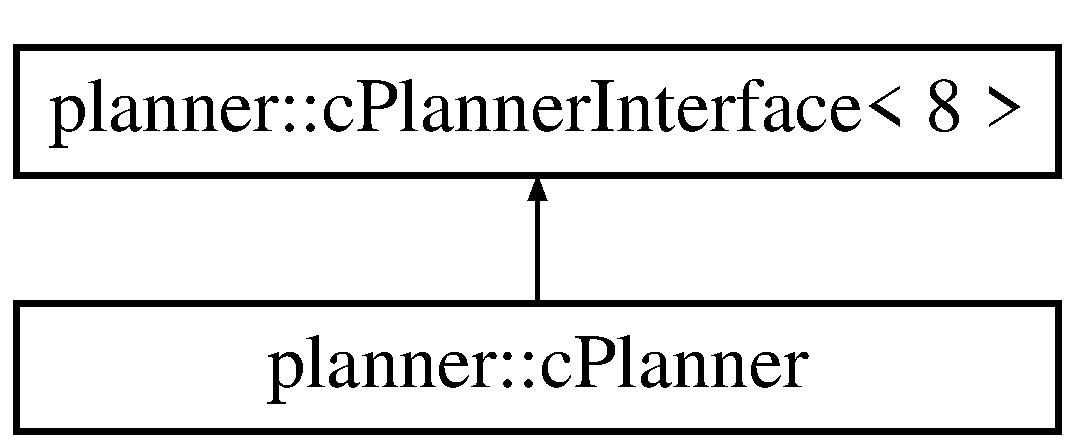
\includegraphics[height=2.000000cm]{classplanner_1_1c_planner}
\end{center}
\end{figure}
\subsection*{Public Types}
\begin{DoxyCompactItemize}
\item 
\mbox{\Hypertarget{classplanner_1_1c_planner_a7f6dc4cbb69dd1ede14a67b0a7bd425b}\label{classplanner_1_1c_planner_a7f6dc4cbb69dd1ede14a67b0a7bd425b}} 
enum \mbox{\hyperlink{classplanner_1_1c_planner_a7f6dc4cbb69dd1ede14a67b0a7bd425b}{t\+Heuristic}} \{ {\bfseries M\+A\+N\+H\+A\+T\+T\+EN}, 
{\bfseries E\+U\+C\+L\+I\+D\+E\+AN}, 
{\bfseries O\+C\+T\+I\+LE}, 
{\bfseries C\+H\+E\+B\+Y\+S\+H\+EV}
 \}
\begin{DoxyCompactList}\small\item\em Types of heuristics that can be calculated with \mbox{\hyperlink{classplanner_1_1c_planner_ad32a7c58b885456ced172b66fed854f0}{Update\+Heuristic()}} \end{DoxyCompactList}\end{DoxyCompactItemize}
\subsection*{Public Member Functions}
\begin{DoxyCompactItemize}
\item 
\mbox{\hyperlink{classplanner_1_1c_planner_a4f425d47b277f000d34df04de9995274}{c\+Planner}} (\mbox{\hyperlink{classplanner_1_1c_rover_interface}{c\+Rover\+Interface}}$<$ 8 $>$ $\ast$i\+\_\+po\+Rover, \mbox{\hyperlink{classplanner_1_1c_graph}{c\+Graph}} \&i\+\_\+o\+Map)
\begin{DoxyCompactList}\small\item\em Initializes member variables m\+\_\+po\+Rover and m\+\_\+o\+Map and calls Calculate\+Consistency\+Factor(). \end{DoxyCompactList}\item 
\mbox{\Hypertarget{classplanner_1_1c_planner_aa9ae1109d3c4b7ac19aef2616547654e}\label{classplanner_1_1c_planner_aa9ae1109d3c4b7ac19aef2616547654e}} 
\mbox{\hyperlink{classplanner_1_1c_planner_aa9ae1109d3c4b7ac19aef2616547654e}{$\sim$c\+Planner}} ()
\begin{DoxyCompactList}\small\item\em Destructor to delete the allocated memory. \end{DoxyCompactList}\item 
float \mbox{\hyperlink{classplanner_1_1c_planner_a7c4defd454429503d4e47b552a5311fb}{Plan}} () override
\begin{DoxyCompactList}\small\item\em Override of the base interface \mbox{\hyperlink{classplanner_1_1c_planner_interface}{c\+Planner\+Interface}}, which invokes the A\+Star() search algorithm. \end{DoxyCompactList}\item 
void \mbox{\hyperlink{classplanner_1_1c_planner_a1a4650050656545744796296a653d388}{Generate\+Heuristic}} ()
\begin{DoxyCompactList}\small\item\em Output distance heuristic map to file, which is used to generate the Matlab plot. \end{DoxyCompactList}\item 
float \mbox{\hyperlink{classplanner_1_1c_planner_ad32a7c58b885456ced172b66fed854f0}{Update\+Heuristic}} (\mbox{\hyperlink{structplanner_1_1t_node}{t\+Node}} $\ast$i\+\_\+s\+Node, const \mbox{\hyperlink{classplanner_1_1c_planner_a7f6dc4cbb69dd1ede14a67b0a7bd425b}{t\+Heuristic}} i\+\_\+e\+Heuristic=O\+C\+T\+I\+LE) const
\begin{DoxyCompactList}\small\item\em Updates the heuristic value of the node argument i\+\_\+s\+Node. \end{DoxyCompactList}\item 
float \mbox{\hyperlink{classplanner_1_1c_planner_a7d5f7f89a10b66f19c0257cbf7f2afbb}{Update\+Heuristic}} (const \mbox{\hyperlink{structplanner_1_1t_location}{t\+Location}} \&i\+\_\+s\+Location, const \mbox{\hyperlink{classplanner_1_1c_planner_a7f6dc4cbb69dd1ede14a67b0a7bd425b}{t\+Heuristic}} i\+\_\+e\+Heuristic=O\+C\+T\+I\+LE) const
\begin{DoxyCompactList}\small\item\em Updates the heuristic value of the node located at tlocation i\+\_\+s\+Location. \end{DoxyCompactList}\item 
void \mbox{\hyperlink{classplanner_1_1c_planner_a8b4f67bd192db4784c6ab95c11e51a16}{Heuristic\+Check}} (\mbox{\hyperlink{structplanner_1_1t_node}{t\+Node}} $\ast$i\+\_\+s\+Node) const
\begin{DoxyCompactList}\small\item\em Check if the heuristic of node i\+\_\+s\+Node is consistent. \end{DoxyCompactList}\item 
void \mbox{\hyperlink{classplanner_1_1c_planner_a82e45fc2701e90d3fa9df72f475e455e}{Update\+Cost}} (\mbox{\hyperlink{structplanner_1_1t_node}{t\+Node}} $\ast$i\+\_\+s\+Node) const
\begin{DoxyCompactList}\small\item\em Updates the node argument with its path cost $g(n)$ with island seconds as its unit. \end{DoxyCompactList}\item 
bool \mbox{\hyperlink{classplanner_1_1c_planner_ac5119e3243d9f6747f1da0ed6d356642}{Within\+Map}} (const \mbox{\hyperlink{structplanner_1_1t_location}{t\+Location}} \&i\+\_\+s\+Location) const
\begin{DoxyCompactList}\small\item\em Test if the provided location i\+\_\+s\+Location lies within the map. \end{DoxyCompactList}\item 
virtual bool \mbox{\hyperlink{classplanner_1_1c_planner_a8b241ebd7bb3bde3dd062c50a2a42339}{Goal\+Test}} (const \mbox{\hyperlink{structplanner_1_1t_node}{t\+Node}} $\ast$i\+\_\+s\+First, const \mbox{\hyperlink{structplanner_1_1t_node}{t\+Node}} $\ast$i\+\_\+s\+Second) const override
\begin{DoxyCompactList}\small\item\em Goal test to check if the two provided nodes i\+\_\+s\+First, i\+\_\+s\+Second are equal. \end{DoxyCompactList}\item 
\mbox{\hyperlink{structplanner_1_1t_node}{t\+Node}} $\ast$ \mbox{\hyperlink{classplanner_1_1c_planner_a7ddb18b161e5d59cfe733bce32c31896}{Child}} (\mbox{\hyperlink{structplanner_1_1t_node}{t\+Node}} $\ast$i\+\_\+s\+Parent, const \mbox{\hyperlink{structplanner_1_1t_action}{t\+Action}} \&i\+\_\+s\+Action) const override
\begin{DoxyCompactList}\small\item\em Generate a successor node state given a node i\+\_\+s\+Parent and action i\+\_\+s\+Action. \end{DoxyCompactList}\item 
bool \mbox{\hyperlink{classplanner_1_1c_planner_a34b0582ca32cc235837c0b638b39e3af}{Traversable}} (\mbox{\hyperlink{structplanner_1_1t_node}{t\+Node}} $\ast$i\+\_\+s\+Current, \mbox{\hyperlink{structplanner_1_1t_node}{t\+Node}} $\ast$i\+\_\+s\+Next) const
\begin{DoxyCompactList}\small\item\em considers step size of rover and checks if the path is traversable T\+O\+DO improve comment \end{DoxyCompactList}\item 
void \mbox{\hyperlink{classplanner_1_1c_planner_ad9389067cbc3fa6fb1c2efdf3f344664}{Traverse\+Path}} (\mbox{\hyperlink{structplanner_1_1t_node}{t\+Node}} $\ast$i\+\_\+ps\+Node) const override
\begin{DoxyCompactList}\small\item\em Given the node i\+\_\+ps\+Node the overrides map m\+\_\+po\+Overrides is updated for displaying the path. \end{DoxyCompactList}\item 
\mbox{\Hypertarget{classplanner_1_1c_planner_aa90d751ce544870e4c89494e06fdac6c}\label{classplanner_1_1c_planner_aa90d751ce544870e4c89494e06fdac6c}} 
const int \mbox{\hyperlink{classplanner_1_1c_planner_aa90d751ce544870e4c89494e06fdac6c}{GradX}} (int i\+\_\+nX, int i\+\_\+nY) const
\begin{DoxyCompactList}\small\item\em Calculates the discrete gradient of the map m\+\_\+po\+Map in x direction. \end{DoxyCompactList}\item 
\mbox{\Hypertarget{classplanner_1_1c_planner_a6fd8e8632d78d85ce472322267ba7b36}\label{classplanner_1_1c_planner_a6fd8e8632d78d85ce472322267ba7b36}} 
const int \mbox{\hyperlink{classplanner_1_1c_planner_a6fd8e8632d78d85ce472322267ba7b36}{GradY}} (int i\+\_\+nX, int i\+\_\+nY) const
\begin{DoxyCompactList}\small\item\em Calculates the discrete gradient of the map m\+\_\+po\+Map in y direction. \end{DoxyCompactList}\item 
uint32\+\_\+t \mbox{\hyperlink{classplanner_1_1c_planner_a5ae4464a4d418cda71f4a8133d592c93}{Node\+Hash}} (const \mbox{\hyperlink{structplanner_1_1t_node}{t\+Node}} $\ast$i\+\_\+s\+Node) const
\begin{DoxyCompactList}\small\item\em Calculates the node hash using its location and the width of the map. \end{DoxyCompactList}\end{DoxyCompactItemize}
\subsection*{Additional Inherited Members}


\subsection{Detailed Description}
Implements the planner interface c\+Planner\+Interface$<$size\+\_\+t Directions$>$ with an action vector of size eight. 

\subsection{Constructor \& Destructor Documentation}
\mbox{\Hypertarget{classplanner_1_1c_planner_a4f425d47b277f000d34df04de9995274}\label{classplanner_1_1c_planner_a4f425d47b277f000d34df04de9995274}} 
\index{planner\+::c\+Planner@{planner\+::c\+Planner}!c\+Planner@{c\+Planner}}
\index{c\+Planner@{c\+Planner}!planner\+::c\+Planner@{planner\+::c\+Planner}}
\subsubsection{\texorpdfstring{c\+Planner()}{cPlanner()}}
{\footnotesize\ttfamily planner\+::c\+Planner\+::c\+Planner (\begin{DoxyParamCaption}\item[{\mbox{\hyperlink{classplanner_1_1c_rover_interface}{c\+Rover\+Interface}}$<$ 8 $>$ $\ast$}]{i\+\_\+po\+Rover,  }\item[{\mbox{\hyperlink{classplanner_1_1c_graph}{c\+Graph}} \&}]{i\+\_\+o\+Map }\end{DoxyParamCaption})}



Initializes member variables m\+\_\+po\+Rover and m\+\_\+o\+Map and calls Calculate\+Consistency\+Factor(). 

The 

\subsection{Member Function Documentation}
\mbox{\Hypertarget{classplanner_1_1c_planner_a7ddb18b161e5d59cfe733bce32c31896}\label{classplanner_1_1c_planner_a7ddb18b161e5d59cfe733bce32c31896}} 
\index{planner\+::c\+Planner@{planner\+::c\+Planner}!Child@{Child}}
\index{Child@{Child}!planner\+::c\+Planner@{planner\+::c\+Planner}}
\subsubsection{\texorpdfstring{Child()}{Child()}}
{\footnotesize\ttfamily \mbox{\hyperlink{structplanner_1_1t_node}{t\+Node}} $\ast$ planner\+::c\+Planner\+::\+Child (\begin{DoxyParamCaption}\item[{\mbox{\hyperlink{structplanner_1_1t_node}{t\+Node}} $\ast$}]{i\+\_\+s\+Parent,  }\item[{const \mbox{\hyperlink{structplanner_1_1t_action}{t\+Action}} \&}]{i\+\_\+s\+Action }\end{DoxyParamCaption}) const\hspace{0.3cm}{\ttfamily [override]}, {\ttfamily [virtual]}}



Generate a successor node state given a node i\+\_\+s\+Parent and action i\+\_\+s\+Action. 

Overrides method of the base class inteface c\+Planner\+Interface$<$size\+\_\+t Directions$>$. Defines a new node on the heap and initializes it according to the given action.


\begin{DoxyParams}[1]{Parameters}
\mbox{\tt in}  & {\em i\+\_\+s\+Parent} & node which becomes the parent of the new node. \\
\hline
\mbox{\tt in}  & {\em i\+\_\+s\+Action} & struct of type \mbox{\hyperlink{structplanner_1_1t_action}{t\+Action}} that contains the direction and cost of the action. \\
\hline
\end{DoxyParams}
Calculate hash of node using its location 

Implements \mbox{\hyperlink{classplanner_1_1c_planner_interface_a499d8d3b81b0090318f4f2ea044c084c}{planner\+::c\+Planner\+Interface$<$ 8 $>$}}.

\mbox{\Hypertarget{classplanner_1_1c_planner_a1a4650050656545744796296a653d388}\label{classplanner_1_1c_planner_a1a4650050656545744796296a653d388}} 
\index{planner\+::c\+Planner@{planner\+::c\+Planner}!Generate\+Heuristic@{Generate\+Heuristic}}
\index{Generate\+Heuristic@{Generate\+Heuristic}!planner\+::c\+Planner@{planner\+::c\+Planner}}
\subsubsection{\texorpdfstring{Generate\+Heuristic()}{GenerateHeuristic()}}
{\footnotesize\ttfamily void planner\+::c\+Planner\+::\+Generate\+Heuristic (\begin{DoxyParamCaption}{ }\end{DoxyParamCaption})}



Output distance heuristic map to file, which is used to generate the Matlab plot. 

This implementation calls \mbox{\hyperlink{classplanner_1_1c_planner_ad32a7c58b885456ced172b66fed854f0}{Update\+Heuristic()}} to calculate a distance heuristic. Because the robot can move in eight directions the octile distance heuristic is calculated. Other possible gird map heuristics are Manhatten, Chebyshev and Euclidean. Output octile distance \mbox{\Hypertarget{classplanner_1_1c_planner_a8b241ebd7bb3bde3dd062c50a2a42339}\label{classplanner_1_1c_planner_a8b241ebd7bb3bde3dd062c50a2a42339}} 
\index{planner\+::c\+Planner@{planner\+::c\+Planner}!Goal\+Test@{Goal\+Test}}
\index{Goal\+Test@{Goal\+Test}!planner\+::c\+Planner@{planner\+::c\+Planner}}
\subsubsection{\texorpdfstring{Goal\+Test()}{GoalTest()}}
{\footnotesize\ttfamily bool planner\+::c\+Planner\+::\+Goal\+Test (\begin{DoxyParamCaption}\item[{const \mbox{\hyperlink{structplanner_1_1t_node}{t\+Node}} $\ast$}]{i\+\_\+s\+First,  }\item[{const \mbox{\hyperlink{structplanner_1_1t_node}{t\+Node}} $\ast$}]{i\+\_\+s\+Second }\end{DoxyParamCaption}) const\hspace{0.3cm}{\ttfamily [override]}, {\ttfamily [virtual]}}



Goal test to check if the two provided nodes i\+\_\+s\+First, i\+\_\+s\+Second are equal. 

Note that this check takes the step size m\+\_\+n\+Step\+Size of the rover into account. This allows to set a step size greater than one, which can be used for debugging. 
\begin{DoxyParams}[1]{Parameters}
\mbox{\tt in}  & {\em i\+\_\+s\+First} & could be the current node that needs to be checked. \\
\hline
\mbox{\tt in}  & {\em i\+\_\+s\+Second} & could be the goal node. \\
\hline
\end{DoxyParams}
\begin{DoxyReturn}{Returns}
true or false if the two nodes are equal. 
\end{DoxyReturn}


Implements \mbox{\hyperlink{classplanner_1_1c_planner_interface_aadc6ccb9088f755bd0ec30046bb79e99}{planner\+::c\+Planner\+Interface$<$ 8 $>$}}.

\mbox{\Hypertarget{classplanner_1_1c_planner_a8b4f67bd192db4784c6ab95c11e51a16}\label{classplanner_1_1c_planner_a8b4f67bd192db4784c6ab95c11e51a16}} 
\index{planner\+::c\+Planner@{planner\+::c\+Planner}!Heuristic\+Check@{Heuristic\+Check}}
\index{Heuristic\+Check@{Heuristic\+Check}!planner\+::c\+Planner@{planner\+::c\+Planner}}
\subsubsection{\texorpdfstring{Heuristic\+Check()}{HeuristicCheck()}}
{\footnotesize\ttfamily void planner\+::c\+Planner\+::\+Heuristic\+Check (\begin{DoxyParamCaption}\item[{\mbox{\hyperlink{structplanner_1_1t_node}{t\+Node}} $\ast$}]{i\+\_\+s\+Node }\end{DoxyParamCaption}) const}



Check if the heuristic of node i\+\_\+s\+Node is consistent. 

Consistency is given if h(n) $<$= c(n,p) + h(p), where h(p) is the heuristic of the parent node and c(n,p) are the step costs from parent p to node n. 
\begin{DoxyParams}[1]{Parameters}
\mbox{\tt in}  & {\em i\+\_\+s\+Node} & the node which heuristic value is tested. \\
\hline
\end{DoxyParams}
\mbox{\Hypertarget{classplanner_1_1c_planner_a5ae4464a4d418cda71f4a8133d592c93}\label{classplanner_1_1c_planner_a5ae4464a4d418cda71f4a8133d592c93}} 
\index{planner\+::c\+Planner@{planner\+::c\+Planner}!Node\+Hash@{Node\+Hash}}
\index{Node\+Hash@{Node\+Hash}!planner\+::c\+Planner@{planner\+::c\+Planner}}
\subsubsection{\texorpdfstring{Node\+Hash()}{NodeHash()}}
{\footnotesize\ttfamily uint32\+\_\+t planner\+::c\+Planner\+::\+Node\+Hash (\begin{DoxyParamCaption}\item[{const \mbox{\hyperlink{structplanner_1_1t_node}{t\+Node}} $\ast$}]{i\+\_\+s\+Node }\end{DoxyParamCaption}) const}



Calculates the node hash using its location and the width of the map. 

The hash is required to sort the std\+::map$<$t\+Node$>$ o\+Cost of reaching a node, which is used in the A\+Star() search algorithm. \mbox{\Hypertarget{classplanner_1_1c_planner_a7c4defd454429503d4e47b552a5311fb}\label{classplanner_1_1c_planner_a7c4defd454429503d4e47b552a5311fb}} 
\index{planner\+::c\+Planner@{planner\+::c\+Planner}!Plan@{Plan}}
\index{Plan@{Plan}!planner\+::c\+Planner@{planner\+::c\+Planner}}
\subsubsection{\texorpdfstring{Plan()}{Plan()}}
{\footnotesize\ttfamily float planner\+::c\+Planner\+::\+Plan (\begin{DoxyParamCaption}{ }\end{DoxyParamCaption})\hspace{0.3cm}{\ttfamily [override]}, {\ttfamily [virtual]}}



Override of the base interface \mbox{\hyperlink{classplanner_1_1c_planner_interface}{c\+Planner\+Interface}}, which invokes the A\+Star() search algorithm. 

\begin{DoxyReturn}{Returns}
the time to travel from start to goal if it was found. Otherwise -\/1 is returned. 
\end{DoxyReturn}


Implements \mbox{\hyperlink{classplanner_1_1c_planner_interface_a4d8effce5ee5d097a30465280e9416d6}{planner\+::c\+Planner\+Interface$<$ 8 $>$}}.

\mbox{\Hypertarget{classplanner_1_1c_planner_a34b0582ca32cc235837c0b638b39e3af}\label{classplanner_1_1c_planner_a34b0582ca32cc235837c0b638b39e3af}} 
\index{planner\+::c\+Planner@{planner\+::c\+Planner}!Traversable@{Traversable}}
\index{Traversable@{Traversable}!planner\+::c\+Planner@{planner\+::c\+Planner}}
\subsubsection{\texorpdfstring{Traversable()}{Traversable()}}
{\footnotesize\ttfamily bool planner\+::c\+Planner\+::\+Traversable (\begin{DoxyParamCaption}\item[{\mbox{\hyperlink{structplanner_1_1t_node}{t\+Node}} $\ast$}]{i\+\_\+s\+Current,  }\item[{\mbox{\hyperlink{structplanner_1_1t_node}{t\+Node}} $\ast$}]{i\+\_\+s\+Next }\end{DoxyParamCaption}) const}



considers step size of rover and checks if the path is traversable T\+O\+DO improve comment 

Check if the intermediate locations moving from current node to next are on mainland or water

Next location lies outside the map \mbox{\Hypertarget{classplanner_1_1c_planner_ad9389067cbc3fa6fb1c2efdf3f344664}\label{classplanner_1_1c_planner_ad9389067cbc3fa6fb1c2efdf3f344664}} 
\index{planner\+::c\+Planner@{planner\+::c\+Planner}!Traverse\+Path@{Traverse\+Path}}
\index{Traverse\+Path@{Traverse\+Path}!planner\+::c\+Planner@{planner\+::c\+Planner}}
\subsubsection{\texorpdfstring{Traverse\+Path()}{TraversePath()}}
{\footnotesize\ttfamily void planner\+::c\+Planner\+::\+Traverse\+Path (\begin{DoxyParamCaption}\item[{\mbox{\hyperlink{structplanner_1_1t_node}{t\+Node}} $\ast$}]{i\+\_\+ps\+Node }\end{DoxyParamCaption}) const\hspace{0.3cm}{\ttfamily [override]}, {\ttfamily [virtual]}}



Given the node i\+\_\+ps\+Node the overrides map m\+\_\+po\+Overrides is updated for displaying the path. 

Traversing a path takes place using the m\+\_\+ps\+Parent field of the \mbox{\hyperlink{structplanner_1_1t_node}{t\+Node}} struct. 
\begin{DoxyParams}[1]{Parameters}
\mbox{\tt in}  & {\em i\+\_\+ps\+Node} & Goal node or any other which is traversed back \\
\hline
\end{DoxyParams}
Check if the current node is the start node, which has no parent and is therefore set to N\+U\+LL

Store path in overrides

Move towards the start 

Implements \mbox{\hyperlink{classplanner_1_1c_planner_interface_a5c30b547b681b04434102fbcc7c72ea3}{planner\+::c\+Planner\+Interface$<$ 8 $>$}}.

\mbox{\Hypertarget{classplanner_1_1c_planner_a82e45fc2701e90d3fa9df72f475e455e}\label{classplanner_1_1c_planner_a82e45fc2701e90d3fa9df72f475e455e}} 
\index{planner\+::c\+Planner@{planner\+::c\+Planner}!Update\+Cost@{Update\+Cost}}
\index{Update\+Cost@{Update\+Cost}!planner\+::c\+Planner@{planner\+::c\+Planner}}
\subsubsection{\texorpdfstring{Update\+Cost()}{UpdateCost()}}
{\footnotesize\ttfamily void planner\+::c\+Planner\+::\+Update\+Cost (\begin{DoxyParamCaption}\item[{\mbox{\hyperlink{structplanner_1_1t_node}{t\+Node}} $\ast$}]{i\+\_\+s\+Node }\end{DoxyParamCaption}) const}



Updates the node argument with its path cost $g(n)$ with island seconds as its unit. 

Uses the slope found from the gradient of the elevation map c\+Map\+::m\+\_\+o\+Elevation to calculate an acceleration value, where only its component in the x,y plane is used. The value is added to the time it takes for a straight or diagonal step (depending on the action of the node). The sum is stored in $g(n)$ of the node \mbox{\hyperlink{structplanner_1_1t_node}{planner\+::t\+Node}} i\+\_\+s\+Node. 
\begin{DoxyParams}[1]{Parameters}
\mbox{\tt in}  & {\em i\+\_\+s\+Node} & The node which path cost is updated. \\
\hline
\end{DoxyParams}
Rover\textquotesingle{}s normal speed is 1 cell per island second

Add action (step) cost, which is given in island seconds

If the rover is going up or down hill, calculate the acceleration on the inclined plane Calculate current gradient in step direction ~\newline
 Down hill \mbox{\Hypertarget{classplanner_1_1c_planner_ad32a7c58b885456ced172b66fed854f0}\label{classplanner_1_1c_planner_ad32a7c58b885456ced172b66fed854f0}} 
\index{planner\+::c\+Planner@{planner\+::c\+Planner}!Update\+Heuristic@{Update\+Heuristic}}
\index{Update\+Heuristic@{Update\+Heuristic}!planner\+::c\+Planner@{planner\+::c\+Planner}}
\subsubsection{\texorpdfstring{Update\+Heuristic()}{UpdateHeuristic()}\hspace{0.1cm}{\footnotesize\ttfamily [1/2]}}
{\footnotesize\ttfamily float planner\+::c\+Planner\+::\+Update\+Heuristic (\begin{DoxyParamCaption}\item[{\mbox{\hyperlink{structplanner_1_1t_node}{t\+Node}} $\ast$}]{i\+\_\+s\+Node,  }\item[{const \mbox{\hyperlink{classplanner_1_1c_planner_a7f6dc4cbb69dd1ede14a67b0a7bd425b}{t\+Heuristic}}}]{i\+\_\+e\+Heuristic = {\ttfamily OCTILE} }\end{DoxyParamCaption}) const}



Updates the heuristic value of the node argument i\+\_\+s\+Node. 

Calcualtes a grid map distance heuristic. Can be one of the heuristics defined in t\+Heuristic. 
\begin{DoxyParams}[1]{Parameters}
\mbox{\tt in}  & {\em i\+\_\+s\+Node} & the node which heuristic is updated \\
\hline
\mbox{\tt in}  & {\em i\+\_\+e\+Heuristic} & the type of heuristic to calculate, see t\+Heuristic. \\
\hline
\end{DoxyParams}
\begin{DoxyReturn}{Returns}
The calculated heuristic value. 
\end{DoxyReturn}
Correct heuristic value to get a consistent heuristic. Required because of moving up or down the hill. \mbox{\Hypertarget{classplanner_1_1c_planner_a7d5f7f89a10b66f19c0257cbf7f2afbb}\label{classplanner_1_1c_planner_a7d5f7f89a10b66f19c0257cbf7f2afbb}} 
\index{planner\+::c\+Planner@{planner\+::c\+Planner}!Update\+Heuristic@{Update\+Heuristic}}
\index{Update\+Heuristic@{Update\+Heuristic}!planner\+::c\+Planner@{planner\+::c\+Planner}}
\subsubsection{\texorpdfstring{Update\+Heuristic()}{UpdateHeuristic()}\hspace{0.1cm}{\footnotesize\ttfamily [2/2]}}
{\footnotesize\ttfamily float planner\+::c\+Planner\+::\+Update\+Heuristic (\begin{DoxyParamCaption}\item[{const \mbox{\hyperlink{structplanner_1_1t_location}{t\+Location}} \&}]{i\+\_\+s\+Location,  }\item[{const \mbox{\hyperlink{classplanner_1_1c_planner_a7f6dc4cbb69dd1ede14a67b0a7bd425b}{t\+Heuristic}}}]{i\+\_\+e\+Heuristic = {\ttfamily OCTILE} }\end{DoxyParamCaption}) const}



Updates the heuristic value of the node located at tlocation i\+\_\+s\+Location. 

Calcualtes a grid map distance heuristic. Can be one of the heuristics defined in t\+Heuristic. 
\begin{DoxyParams}[1]{Parameters}
\mbox{\tt in}  & {\em i\+\_\+s\+Node} & the node which heuristic is updated \\
\hline
\mbox{\tt in}  & {\em i\+\_\+e\+Heuristic} & the type of heuristic to calculate, see t\+Heuristic. \\
\hline
\end{DoxyParams}
\begin{DoxyReturn}{Returns}
The calculated heuristic value. 
\end{DoxyReturn}
Manhattan Distance

Euclidian Distance

Octile distance

Euclidian Distance \mbox{\Hypertarget{classplanner_1_1c_planner_ac5119e3243d9f6747f1da0ed6d356642}\label{classplanner_1_1c_planner_ac5119e3243d9f6747f1da0ed6d356642}} 
\index{planner\+::c\+Planner@{planner\+::c\+Planner}!Within\+Map@{Within\+Map}}
\index{Within\+Map@{Within\+Map}!planner\+::c\+Planner@{planner\+::c\+Planner}}
\subsubsection{\texorpdfstring{Within\+Map()}{WithinMap()}}
{\footnotesize\ttfamily bool planner\+::c\+Planner\+::\+Within\+Map (\begin{DoxyParamCaption}\item[{const \mbox{\hyperlink{structplanner_1_1t_location}{t\+Location}} \&}]{i\+\_\+s\+Location }\end{DoxyParamCaption}) const}



Test if the provided location i\+\_\+s\+Location lies within the map. 

Checks if the provided location lies within the map height and width and if the location is equal or greater than zero. 
\begin{DoxyParams}[1]{Parameters}
\mbox{\tt in}  & {\em i\+\_\+s\+Location} & the location of type \mbox{\hyperlink{structplanner_1_1t_location}{t\+Location}}. \\
\hline
\end{DoxyParams}
\begin{DoxyReturn}{Returns}
true if the location i\+\_\+s\+Location lies within the map otherwise false. 
\end{DoxyReturn}


The documentation for this class was generated from the following files\+:\begin{DoxyCompactItemize}
\item 
/\+Users/fjp/git/bachelor/planner/include/planner.\+h\item 
/\+Users/fjp/git/bachelor/planner/src/planner.\+cpp\end{DoxyCompactItemize}

\hypertarget{classplanner_1_1c_planner_interface}{}\section{planner\+:\+:c\+Planner\+Interface$<$ Directions $>$ Class Template Reference}
\label{classplanner_1_1c_planner_interface}\index{planner\+::c\+Planner\+Interface$<$ Directions $>$@{planner\+::c\+Planner\+Interface$<$ Directions $>$}}


\mbox{\hyperlink{classplanner_1_1c_planner_interface}{c\+Planner\+Interface}} is an abstract interface which can be implemented by concrete planner classes.  




{\ttfamily \#include $<$planner\+\_\+interface.\+h$>$}

\subsection*{Public Member Functions}
\begin{DoxyCompactItemize}
\item 
\mbox{\Hypertarget{classplanner_1_1c_planner_interface_a2d99a6f9fe144a0406c040d8da2a6dd4}\label{classplanner_1_1c_planner_interface_a2d99a6f9fe144a0406c040d8da2a6dd4}} 
\mbox{\hyperlink{classplanner_1_1c_planner_interface_a2d99a6f9fe144a0406c040d8da2a6dd4}{c\+Planner\+Interface}} (std\+::shared\+\_\+ptr$<$ \mbox{\hyperlink{classplanner_1_1c_rover_interface}{c\+Rover\+Interface}}$<$ Directions $>$$>$ i\+\_\+po\+Rover, std\+::shared\+\_\+ptr$<$ \mbox{\hyperlink{classplanner_1_1c_graph}{c\+Graph}} $>$ i\+\_\+o\+Map)
\begin{DoxyCompactList}\small\item\em The constructor of the interface which initializes its members m\+\_\+po\+Rover and m\+\_\+o\+Map. \end{DoxyCompactList}\item 
virtual \mbox{\hyperlink{structt_result}{t\+Result}} \mbox{\hyperlink{classplanner_1_1c_planner_interface_a7a06632a8c53906daf39611d9692ffa5}{Plan}} ()=0
\begin{DoxyCompactList}\small\item\em Virtual abstract method of the base interface, which must be implemented to perform a search algorithm. \end{DoxyCompactList}\item 
virtual bool \mbox{\hyperlink{classplanner_1_1c_planner_interface_afec836d58ce54c49046bf30ecdebbfec}{Goal\+Test}} (std\+::shared\+\_\+ptr$<$ \mbox{\hyperlink{structplanner_1_1t_node}{t\+Node}} $>$ \&i\+\_\+s\+First, std\+::shared\+\_\+ptr$<$ \mbox{\hyperlink{structplanner_1_1t_node}{t\+Node}} $>$ \&i\+\_\+s\+Second) const =0
\begin{DoxyCompactList}\small\item\em Test if two nodes are the same, which means the goal is reached. \end{DoxyCompactList}\item 
virtual std\+::shared\+\_\+ptr$<$ \mbox{\hyperlink{structplanner_1_1t_node}{t\+Node}} $>$ \mbox{\hyperlink{classplanner_1_1c_planner_interface_a7e2048c2a4c699a76db90d1cbfecf156}{Child}} (std\+::shared\+\_\+ptr$<$ \mbox{\hyperlink{structplanner_1_1t_node}{t\+Node}} $>$ \&i\+\_\+s\+Parent, const \mbox{\hyperlink{structplanner_1_1t_action}{t\+Action}} \&i\+\_\+s\+Action) const =0
\begin{DoxyCompactList}\small\item\em Given the action i\+\_\+s\+Action and the parent node i\+\_\+s\+Parent a new node of type \mbox{\hyperlink{structplanner_1_1t_node}{t\+Node}} is created. \end{DoxyCompactList}\item 
\mbox{\Hypertarget{classplanner_1_1c_planner_interface_af7a88d017115e9bfee25c12091062641}\label{classplanner_1_1c_planner_interface_af7a88d017115e9bfee25c12091062641}} 
\mbox{\hyperlink{structt_result}{t\+Result}} \mbox{\hyperlink{classplanner_1_1c_planner_interface_af7a88d017115e9bfee25c12091062641}{Result}} ()
\begin{DoxyCompactList}\small\item\em Getter to obtain result struct member m\+\_\+s\+Result that contains information about the found path. \end{DoxyCompactList}\item 
\mbox{\Hypertarget{classplanner_1_1c_planner_interface_ae09e9120335fce8f331749f492255fca}\label{classplanner_1_1c_planner_interface_ae09e9120335fce8f331749f492255fca}} 
\mbox{\hyperlink{classplanner_1_1c_planner_interface_ae09e9120335fce8f331749f492255fca}{c\+Planner\+Interface}} (std\+::shared\+\_\+ptr$<$ \mbox{\hyperlink{classplanner_1_1c_rover_interface}{c\+Rover\+Interface}}$<$ Directions $>$$>$ i\+\_\+po\+Rover, std\+::shared\+\_\+ptr$<$ \mbox{\hyperlink{classplanner_1_1c_graph}{c\+Graph}} $>$ i\+\_\+po\+Map)
\begin{DoxyCompactList}\small\item\em The constructor of the interface which initializes its members m\+\_\+po\+Rover and m\+\_\+o\+Map. \end{DoxyCompactList}\item 
virtual \mbox{\hyperlink{structt_result}{t\+Result}} \mbox{\hyperlink{classplanner_1_1c_planner_interface_a7a06632a8c53906daf39611d9692ffa5}{Plan}} ()=0
\begin{DoxyCompactList}\small\item\em Virtual abstract method of the base interface, which must be implemented to perform a search algorithm. \end{DoxyCompactList}\item 
virtual bool \mbox{\hyperlink{classplanner_1_1c_planner_interface_afec836d58ce54c49046bf30ecdebbfec}{Goal\+Test}} (std\+::shared\+\_\+ptr$<$ \mbox{\hyperlink{structplanner_1_1t_node}{t\+Node}} $>$ \&i\+\_\+s\+First, std\+::shared\+\_\+ptr$<$ \mbox{\hyperlink{structplanner_1_1t_node}{t\+Node}} $>$ \&i\+\_\+s\+Second) const =0
\begin{DoxyCompactList}\small\item\em Test if two nodes are the same, which means the goal is reached. \end{DoxyCompactList}\item 
virtual std\+::shared\+\_\+ptr$<$ \mbox{\hyperlink{structplanner_1_1t_node}{t\+Node}} $>$ \mbox{\hyperlink{classplanner_1_1c_planner_interface_a7e2048c2a4c699a76db90d1cbfecf156}{Child}} (std\+::shared\+\_\+ptr$<$ \mbox{\hyperlink{structplanner_1_1t_node}{t\+Node}} $>$ \&i\+\_\+s\+Parent, const \mbox{\hyperlink{structplanner_1_1t_action}{t\+Action}} \&i\+\_\+s\+Action) const =0
\begin{DoxyCompactList}\small\item\em Given the action i\+\_\+s\+Action and the parent node i\+\_\+s\+Parent a new node of type \mbox{\hyperlink{structplanner_1_1t_node}{t\+Node}} is created. \end{DoxyCompactList}\item 
\mbox{\Hypertarget{classplanner_1_1c_planner_interface_af7a88d017115e9bfee25c12091062641}\label{classplanner_1_1c_planner_interface_af7a88d017115e9bfee25c12091062641}} 
\mbox{\hyperlink{structt_result}{t\+Result}} \mbox{\hyperlink{classplanner_1_1c_planner_interface_af7a88d017115e9bfee25c12091062641}{Result}} ()
\begin{DoxyCompactList}\small\item\em Getter to obtain result struct member m\+\_\+s\+Result that contains information about the found path. \end{DoxyCompactList}\end{DoxyCompactItemize}
\subsection*{Protected Attributes}
\begin{DoxyCompactItemize}
\item 
\mbox{\Hypertarget{classplanner_1_1c_planner_interface_a78389ea53bd3c9d5c57851a338ee91d8}\label{classplanner_1_1c_planner_interface_a78389ea53bd3c9d5c57851a338ee91d8}} 
\mbox{\hyperlink{structt_result}{t\+Result}} \mbox{\hyperlink{classplanner_1_1c_planner_interface_a78389ea53bd3c9d5c57851a338ee91d8}{m\+\_\+s\+Result}}
\begin{DoxyCompactList}\small\item\em Information to store planning results such as travelling time and consistency of heuristic. \end{DoxyCompactList}\item 
\mbox{\Hypertarget{classplanner_1_1c_planner_interface_a4ef4a42f9e26463899f7c54d06580d7f}\label{classplanner_1_1c_planner_interface_a4ef4a42f9e26463899f7c54d06580d7f}} 
std\+::shared\+\_\+ptr$<$ \mbox{\hyperlink{classplanner_1_1c_rover_interface}{c\+Rover\+Interface}}$<$ Directions $>$ $>$ \mbox{\hyperlink{classplanner_1_1c_planner_interface_a4ef4a42f9e26463899f7c54d06580d7f}{m\+\_\+po\+Rover}}
\begin{DoxyCompactList}\small\item\em Reference pointer to the interface of the rover class planner\+::c\+Rover\+Interface$<$\+Directions$>$. \end{DoxyCompactList}\item 
\mbox{\Hypertarget{classplanner_1_1c_planner_interface_a5145c31369e5092bfcfc836de75a5680}\label{classplanner_1_1c_planner_interface_a5145c31369e5092bfcfc836de75a5680}} 
std\+::shared\+\_\+ptr$<$ \mbox{\hyperlink{classplanner_1_1c_graph}{c\+Graph}} $>$ \mbox{\hyperlink{classplanner_1_1c_planner_interface_a5145c31369e5092bfcfc836de75a5680}{m\+\_\+o\+Map}}
\begin{DoxyCompactList}\small\item\em Provides the subclasses with important map information such as terrain and elevation maps. \end{DoxyCompactList}\item 
\mbox{\Hypertarget{classplanner_1_1c_planner_interface_aa75ba58312d9398785d541a5e580a665}\label{classplanner_1_1c_planner_interface_aa75ba58312d9398785d541a5e580a665}} 
std\+::shared\+\_\+ptr$<$ \mbox{\hyperlink{classplanner_1_1c_graph}{c\+Graph}} $>$ \mbox{\hyperlink{classplanner_1_1c_planner_interface_aa75ba58312d9398785d541a5e580a665}{m\+\_\+po\+Map}}
\begin{DoxyCompactList}\small\item\em Provides the subclasses with important map information such as terrain and elevation maps. \end{DoxyCompactList}\end{DoxyCompactItemize}


\subsection{Detailed Description}
\subsubsection*{template$<$size\+\_\+t Directions$>$\newline
class planner\+::c\+Planner\+Interface$<$ Directions $>$}

\mbox{\hyperlink{classplanner_1_1c_planner_interface}{c\+Planner\+Interface}} is an abstract interface which can be implemented by concrete planner classes. 

Forward declaration of planner interface. 

\subsection{Member Function Documentation}
\mbox{\Hypertarget{classplanner_1_1c_planner_interface_a7e2048c2a4c699a76db90d1cbfecf156}\label{classplanner_1_1c_planner_interface_a7e2048c2a4c699a76db90d1cbfecf156}} 
\index{planner\+::c\+Planner\+Interface@{planner\+::c\+Planner\+Interface}!Child@{Child}}
\index{Child@{Child}!planner\+::c\+Planner\+Interface@{planner\+::c\+Planner\+Interface}}
\subsubsection{\texorpdfstring{Child()}{Child()}\hspace{0.1cm}{\footnotesize\ttfamily [1/2]}}
{\footnotesize\ttfamily template$<$size\+\_\+t Directions$>$ \\
virtual std\+::shared\+\_\+ptr$<$\mbox{\hyperlink{structplanner_1_1t_node}{t\+Node}}$>$ \mbox{\hyperlink{classplanner_1_1c_planner_interface}{planner\+::c\+Planner\+Interface}}$<$ Directions $>$\+::Child (\begin{DoxyParamCaption}\item[{std\+::shared\+\_\+ptr$<$ \mbox{\hyperlink{structplanner_1_1t_node}{t\+Node}} $>$ \&}]{i\+\_\+s\+Parent,  }\item[{const \mbox{\hyperlink{structplanner_1_1t_action}{t\+Action}} \&}]{i\+\_\+s\+Action }\end{DoxyParamCaption}) const\hspace{0.3cm}{\ttfamily [pure virtual]}}



Given the action i\+\_\+s\+Action and the parent node i\+\_\+s\+Parent a new node of type \mbox{\hyperlink{structplanner_1_1t_node}{t\+Node}} is created. 

Defined pure virtual which means it must be implemented by the subclasses the inherit from this interface. 

Implemented in \mbox{\hyperlink{classplanner_1_1c_planner_adbffc6ce05119c940a09369d7e61554e}{planner\+::c\+Planner}}, and \mbox{\hyperlink{classplanner_1_1c_planner_ab260cfcb0ad00d46b02148d19faf040d}{planner\+::c\+Planner}}.

\mbox{\Hypertarget{classplanner_1_1c_planner_interface_a7e2048c2a4c699a76db90d1cbfecf156}\label{classplanner_1_1c_planner_interface_a7e2048c2a4c699a76db90d1cbfecf156}} 
\index{planner\+::c\+Planner\+Interface@{planner\+::c\+Planner\+Interface}!Child@{Child}}
\index{Child@{Child}!planner\+::c\+Planner\+Interface@{planner\+::c\+Planner\+Interface}}
\subsubsection{\texorpdfstring{Child()}{Child()}\hspace{0.1cm}{\footnotesize\ttfamily [2/2]}}
{\footnotesize\ttfamily template$<$size\+\_\+t Directions$>$ \\
virtual std\+::shared\+\_\+ptr$<$\mbox{\hyperlink{structplanner_1_1t_node}{t\+Node}}$>$ \mbox{\hyperlink{classplanner_1_1c_planner_interface}{planner\+::c\+Planner\+Interface}}$<$ Directions $>$\+::Child (\begin{DoxyParamCaption}\item[{std\+::shared\+\_\+ptr$<$ \mbox{\hyperlink{structplanner_1_1t_node}{t\+Node}} $>$ \&}]{i\+\_\+s\+Parent,  }\item[{const \mbox{\hyperlink{structplanner_1_1t_action}{t\+Action}} \&}]{i\+\_\+s\+Action }\end{DoxyParamCaption}) const\hspace{0.3cm}{\ttfamily [pure virtual]}}



Given the action i\+\_\+s\+Action and the parent node i\+\_\+s\+Parent a new node of type \mbox{\hyperlink{structplanner_1_1t_node}{t\+Node}} is created. 

Defined pure virtual which means it must be implemented by the subclasses the inherit from this interface. 

Implemented in \mbox{\hyperlink{classplanner_1_1c_planner_adbffc6ce05119c940a09369d7e61554e}{planner\+::c\+Planner}}, and \mbox{\hyperlink{classplanner_1_1c_planner_ab260cfcb0ad00d46b02148d19faf040d}{planner\+::c\+Planner}}.

\mbox{\Hypertarget{classplanner_1_1c_planner_interface_afec836d58ce54c49046bf30ecdebbfec}\label{classplanner_1_1c_planner_interface_afec836d58ce54c49046bf30ecdebbfec}} 
\index{planner\+::c\+Planner\+Interface@{planner\+::c\+Planner\+Interface}!Goal\+Test@{Goal\+Test}}
\index{Goal\+Test@{Goal\+Test}!planner\+::c\+Planner\+Interface@{planner\+::c\+Planner\+Interface}}
\subsubsection{\texorpdfstring{Goal\+Test()}{GoalTest()}\hspace{0.1cm}{\footnotesize\ttfamily [1/2]}}
{\footnotesize\ttfamily template$<$size\+\_\+t Directions$>$ \\
virtual bool \mbox{\hyperlink{classplanner_1_1c_planner_interface}{planner\+::c\+Planner\+Interface}}$<$ Directions $>$\+::Goal\+Test (\begin{DoxyParamCaption}\item[{std\+::shared\+\_\+ptr$<$ \mbox{\hyperlink{structplanner_1_1t_node}{t\+Node}} $>$ \&}]{i\+\_\+s\+First,  }\item[{std\+::shared\+\_\+ptr$<$ \mbox{\hyperlink{structplanner_1_1t_node}{t\+Node}} $>$ \&}]{i\+\_\+s\+Second }\end{DoxyParamCaption}) const\hspace{0.3cm}{\ttfamily [pure virtual]}}



Test if two nodes are the same, which means the goal is reached. 

Defined pure virtual which means it must be implemented by the subclasses the inherit from this interface. 

Implemented in \mbox{\hyperlink{classplanner_1_1c_planner_a6b7554394efd7ad10d76a49b370aa62f}{planner\+::c\+Planner}}, and \mbox{\hyperlink{classplanner_1_1c_planner_a7050795c7174d0ec427fc91f8756a3d8}{planner\+::c\+Planner}}.

\mbox{\Hypertarget{classplanner_1_1c_planner_interface_afec836d58ce54c49046bf30ecdebbfec}\label{classplanner_1_1c_planner_interface_afec836d58ce54c49046bf30ecdebbfec}} 
\index{planner\+::c\+Planner\+Interface@{planner\+::c\+Planner\+Interface}!Goal\+Test@{Goal\+Test}}
\index{Goal\+Test@{Goal\+Test}!planner\+::c\+Planner\+Interface@{planner\+::c\+Planner\+Interface}}
\subsubsection{\texorpdfstring{Goal\+Test()}{GoalTest()}\hspace{0.1cm}{\footnotesize\ttfamily [2/2]}}
{\footnotesize\ttfamily template$<$size\+\_\+t Directions$>$ \\
virtual bool \mbox{\hyperlink{classplanner_1_1c_planner_interface}{planner\+::c\+Planner\+Interface}}$<$ Directions $>$\+::Goal\+Test (\begin{DoxyParamCaption}\item[{std\+::shared\+\_\+ptr$<$ \mbox{\hyperlink{structplanner_1_1t_node}{t\+Node}} $>$ \&}]{i\+\_\+s\+First,  }\item[{std\+::shared\+\_\+ptr$<$ \mbox{\hyperlink{structplanner_1_1t_node}{t\+Node}} $>$ \&}]{i\+\_\+s\+Second }\end{DoxyParamCaption}) const\hspace{0.3cm}{\ttfamily [pure virtual]}}



Test if two nodes are the same, which means the goal is reached. 

Defined pure virtual which means it must be implemented by the subclasses the inherit from this interface. 

Implemented in \mbox{\hyperlink{classplanner_1_1c_planner_a6b7554394efd7ad10d76a49b370aa62f}{planner\+::c\+Planner}}, and \mbox{\hyperlink{classplanner_1_1c_planner_a7050795c7174d0ec427fc91f8756a3d8}{planner\+::c\+Planner}}.

\mbox{\Hypertarget{classplanner_1_1c_planner_interface_a7a06632a8c53906daf39611d9692ffa5}\label{classplanner_1_1c_planner_interface_a7a06632a8c53906daf39611d9692ffa5}} 
\index{planner\+::c\+Planner\+Interface@{planner\+::c\+Planner\+Interface}!Plan@{Plan}}
\index{Plan@{Plan}!planner\+::c\+Planner\+Interface@{planner\+::c\+Planner\+Interface}}
\subsubsection{\texorpdfstring{Plan()}{Plan()}\hspace{0.1cm}{\footnotesize\ttfamily [1/2]}}
{\footnotesize\ttfamily template$<$size\+\_\+t Directions$>$ \\
virtual \mbox{\hyperlink{structt_result}{t\+Result}} \mbox{\hyperlink{classplanner_1_1c_planner_interface}{planner\+::c\+Planner\+Interface}}$<$ Directions $>$\+::Plan (\begin{DoxyParamCaption}{ }\end{DoxyParamCaption})\hspace{0.3cm}{\ttfamily [pure virtual]}}



Virtual abstract method of the base interface, which must be implemented to perform a search algorithm. 

\begin{DoxyReturn}{Returns}
The cost to move from start to goal if it was found. Otherwise -\/1 is returned. 
\end{DoxyReturn}


Implemented in \mbox{\hyperlink{classplanner_1_1c_planner_a21230c015260b9fc34ad2f239592470e}{planner\+::c\+Planner}}, \mbox{\hyperlink{classplanner_1_1c_planner_a21230c015260b9fc34ad2f239592470e}{planner\+::c\+Planner}}, \mbox{\hyperlink{classplanner_1_1c_planner_r_b_g_a0bbd752702da582a47dbd153c0065eb5}{planner\+::c\+Planner\+R\+BG}}, \mbox{\hyperlink{classplanner_1_1c_planner_wiki_a9d18be721400b51162ff463ab11d1721}{planner\+::c\+Planner\+Wiki}}, \mbox{\hyperlink{classplanner_1_1c_planner_r_b_g_a0bbd752702da582a47dbd153c0065eb5}{planner\+::c\+Planner\+R\+BG}}, and \mbox{\hyperlink{classplanner_1_1c_planner_wiki_a9d18be721400b51162ff463ab11d1721}{planner\+::c\+Planner\+Wiki}}.

\mbox{\Hypertarget{classplanner_1_1c_planner_interface_a7a06632a8c53906daf39611d9692ffa5}\label{classplanner_1_1c_planner_interface_a7a06632a8c53906daf39611d9692ffa5}} 
\index{planner\+::c\+Planner\+Interface@{planner\+::c\+Planner\+Interface}!Plan@{Plan}}
\index{Plan@{Plan}!planner\+::c\+Planner\+Interface@{planner\+::c\+Planner\+Interface}}
\subsubsection{\texorpdfstring{Plan()}{Plan()}\hspace{0.1cm}{\footnotesize\ttfamily [2/2]}}
{\footnotesize\ttfamily template$<$size\+\_\+t Directions$>$ \\
virtual \mbox{\hyperlink{structt_result}{t\+Result}} \mbox{\hyperlink{classplanner_1_1c_planner_interface}{planner\+::c\+Planner\+Interface}}$<$ Directions $>$\+::Plan (\begin{DoxyParamCaption}{ }\end{DoxyParamCaption})\hspace{0.3cm}{\ttfamily [pure virtual]}}



Virtual abstract method of the base interface, which must be implemented to perform a search algorithm. 

\begin{DoxyReturn}{Returns}
The cost to move from start to goal if it was found. Otherwise -\/1 is returned. 
\end{DoxyReturn}


Implemented in \mbox{\hyperlink{classplanner_1_1c_planner_a21230c015260b9fc34ad2f239592470e}{planner\+::c\+Planner}}, \mbox{\hyperlink{classplanner_1_1c_planner_a21230c015260b9fc34ad2f239592470e}{planner\+::c\+Planner}}, \mbox{\hyperlink{classplanner_1_1c_planner_r_b_g_a0bbd752702da582a47dbd153c0065eb5}{planner\+::c\+Planner\+R\+BG}}, \mbox{\hyperlink{classplanner_1_1c_planner_wiki_a9d18be721400b51162ff463ab11d1721}{planner\+::c\+Planner\+Wiki}}, \mbox{\hyperlink{classplanner_1_1c_planner_r_b_g_a0bbd752702da582a47dbd153c0065eb5}{planner\+::c\+Planner\+R\+BG}}, and \mbox{\hyperlink{classplanner_1_1c_planner_wiki_a9d18be721400b51162ff463ab11d1721}{planner\+::c\+Planner\+Wiki}}.



The documentation for this class was generated from the following file\+:\begin{DoxyCompactItemize}
\item 
/\+Users/fjp/git/bachelor/bachelor-\/master\+\_\+updated\+\_\+vfinal/planner/include/planner\+\_\+interface.\+h\end{DoxyCompactItemize}

\hypertarget{classplanner_1_1c_planner_r_b_g}{}\section{planner\+:\+:c\+Planner\+R\+BG Class Reference}
\label{classplanner_1_1c_planner_r_b_g}\index{planner\+::c\+Planner\+R\+BG@{planner\+::c\+Planner\+R\+BG}}


Extends the planner class to implement A$\ast$ from Wikipedia.  




{\ttfamily \#include $<$planner\+\_\+rbg.\+h$>$}



Inheritance diagram for planner\+:\+:c\+Planner\+R\+BG\+:
\nopagebreak
\begin{figure}[H]
\begin{center}
\leavevmode
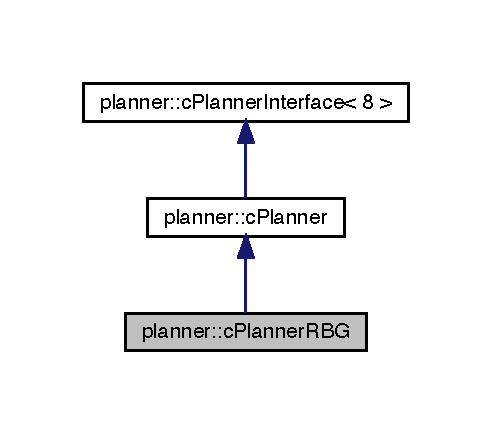
\includegraphics[width=236pt]{classplanner_1_1c_planner_r_b_g__inherit__graph}
\end{center}
\end{figure}


Collaboration diagram for planner\+:\+:c\+Planner\+R\+BG\+:
\nopagebreak
\begin{figure}[H]
\begin{center}
\leavevmode
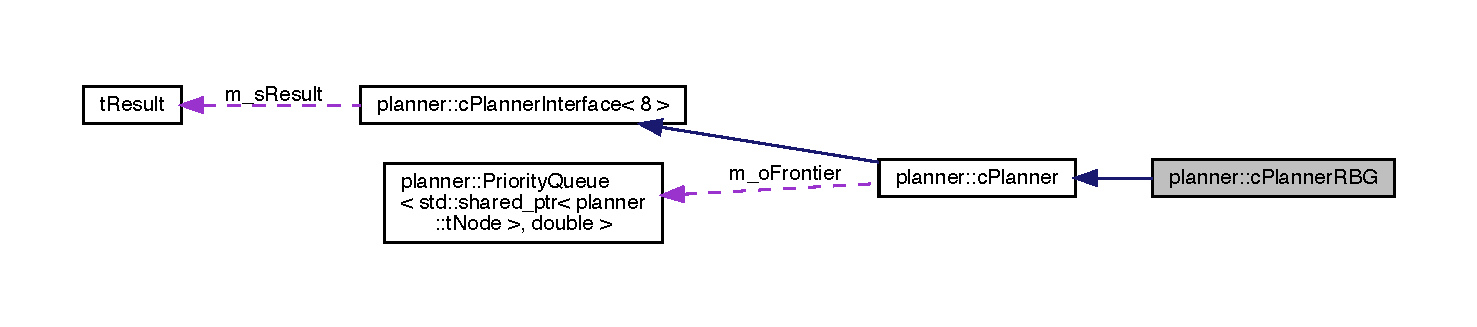
\includegraphics[width=350pt]{classplanner_1_1c_planner_r_b_g__coll__graph}
\end{center}
\end{figure}
\subsection*{Public Member Functions}
\begin{DoxyCompactItemize}
\item 
\mbox{\hyperlink{classplanner_1_1c_planner_r_b_g_a91296b98e64effc16f38e2430746d94d}{c\+Planner\+R\+BG}} (std\+::shared\+\_\+ptr$<$ \mbox{\hyperlink{classplanner_1_1c_rover_interface}{c\+Rover\+Interface}}$<$ 8 $>$$>$ i\+\_\+po\+Rover, std\+::shared\+\_\+ptr$<$ \mbox{\hyperlink{classplanner_1_1c_graph}{c\+Graph}} $>$ i\+\_\+o\+Map)
\begin{DoxyCompactList}\small\item\em Initializes member variables m\+\_\+po\+Rover and m\+\_\+o\+Map and calls \mbox{\hyperlink{classplanner_1_1c_planner_a2e5a745f83f903662eff914d8beddb5e}{Calculate\+Consistency\+Factor()}}. \end{DoxyCompactList}\item 
\mbox{\Hypertarget{classplanner_1_1c_planner_r_b_g_ad582fdf21ae0d86a23e9c25546b66f0e}\label{classplanner_1_1c_planner_r_b_g_ad582fdf21ae0d86a23e9c25546b66f0e}} 
\mbox{\hyperlink{classplanner_1_1c_planner_r_b_g_ad582fdf21ae0d86a23e9c25546b66f0e}{$\sim$c\+Planner\+R\+BG}} ()
\begin{DoxyCompactList}\small\item\em Destructor to delete the allocated memory. \end{DoxyCompactList}\item 
\mbox{\hyperlink{structt_result}{t\+Result}} \mbox{\hyperlink{classplanner_1_1c_planner_r_b_g_a0bbd752702da582a47dbd153c0065eb5}{Plan}} () override
\begin{DoxyCompactList}\small\item\em Override of the base interface \mbox{\hyperlink{classplanner_1_1c_planner_interface}{c\+Planner\+Interface}}, which invokes the A\+Star() search algorithm. \end{DoxyCompactList}\item 
{\footnotesize template$<$typename T\+Cost\+So\+Far , typename T\+Came\+From $>$ }\\void \mbox{\hyperlink{classplanner_1_1c_planner_r_b_g_a1af74d398b286f1e05e6ade495efbbd0}{Reconstruct\+Path}} (T\+Cost\+So\+Far \&\&i\+\_\+cost\+\_\+so\+\_\+far, T\+Came\+From \&\&i\+\_\+came\+\_\+from)
\begin{DoxyCompactList}\small\item\em Given the node i\+\_\+ps\+Node the overrides map m\+\_\+po\+Overrides is updated for displaying the path. \end{DoxyCompactList}\end{DoxyCompactItemize}
\subsection*{Additional Inherited Members}


\subsection{Detailed Description}
Extends the planner class to implement A$\ast$ from Wikipedia. 

\subsection{Constructor \& Destructor Documentation}
\mbox{\Hypertarget{classplanner_1_1c_planner_r_b_g_a91296b98e64effc16f38e2430746d94d}\label{classplanner_1_1c_planner_r_b_g_a91296b98e64effc16f38e2430746d94d}} 
\index{planner\+::c\+Planner\+R\+BG@{planner\+::c\+Planner\+R\+BG}!c\+Planner\+R\+BG@{c\+Planner\+R\+BG}}
\index{c\+Planner\+R\+BG@{c\+Planner\+R\+BG}!planner\+::c\+Planner\+R\+BG@{planner\+::c\+Planner\+R\+BG}}
\subsubsection{\texorpdfstring{c\+Planner\+R\+B\+G()}{cPlannerRBG()}}
{\footnotesize\ttfamily planner\+::c\+Planner\+R\+B\+G\+::c\+Planner\+R\+BG (\begin{DoxyParamCaption}\item[{std\+::shared\+\_\+ptr$<$ \mbox{\hyperlink{classplanner_1_1c_rover_interface}{c\+Rover\+Interface}}$<$ 8 $>$$>$}]{i\+\_\+po\+Rover,  }\item[{std\+::shared\+\_\+ptr$<$ \mbox{\hyperlink{classplanner_1_1c_graph}{c\+Graph}} $>$}]{i\+\_\+o\+Map }\end{DoxyParamCaption})}



Initializes member variables m\+\_\+po\+Rover and m\+\_\+o\+Map and calls \mbox{\hyperlink{classplanner_1_1c_planner_a2e5a745f83f903662eff914d8beddb5e}{Calculate\+Consistency\+Factor()}}. 

The 

\subsection{Member Function Documentation}
\mbox{\Hypertarget{classplanner_1_1c_planner_r_b_g_a0bbd752702da582a47dbd153c0065eb5}\label{classplanner_1_1c_planner_r_b_g_a0bbd752702da582a47dbd153c0065eb5}} 
\index{planner\+::c\+Planner\+R\+BG@{planner\+::c\+Planner\+R\+BG}!Plan@{Plan}}
\index{Plan@{Plan}!planner\+::c\+Planner\+R\+BG@{planner\+::c\+Planner\+R\+BG}}
\subsubsection{\texorpdfstring{Plan()}{Plan()}}
{\footnotesize\ttfamily \mbox{\hyperlink{structt_result}{t\+Result}} planner\+::c\+Planner\+R\+B\+G\+::\+Plan (\begin{DoxyParamCaption}{ }\end{DoxyParamCaption})\hspace{0.3cm}{\ttfamily [override]}, {\ttfamily [virtual]}}



Override of the base interface \mbox{\hyperlink{classplanner_1_1c_planner_interface}{c\+Planner\+Interface}}, which invokes the A\+Star() search algorithm. 

\begin{DoxyReturn}{Returns}
the time to travel from start to goal if it was found. Otherwise -\/1 is returned. 
\end{DoxyReturn}


Reimplemented from \mbox{\hyperlink{classplanner_1_1c_planner_a21230c015260b9fc34ad2f239592470e}{planner\+::c\+Planner}}.

\mbox{\Hypertarget{classplanner_1_1c_planner_r_b_g_a1af74d398b286f1e05e6ade495efbbd0}\label{classplanner_1_1c_planner_r_b_g_a1af74d398b286f1e05e6ade495efbbd0}} 
\index{planner\+::c\+Planner\+R\+BG@{planner\+::c\+Planner\+R\+BG}!Reconstruct\+Path@{Reconstruct\+Path}}
\index{Reconstruct\+Path@{Reconstruct\+Path}!planner\+::c\+Planner\+R\+BG@{planner\+::c\+Planner\+R\+BG}}
\subsubsection{\texorpdfstring{Reconstruct\+Path()}{ReconstructPath()}}
{\footnotesize\ttfamily template$<$typename T\+Cost\+So\+Far , typename T\+Came\+From $>$ \\
void planner\+::c\+Planner\+R\+B\+G\+::\+Reconstruct\+Path (\begin{DoxyParamCaption}\item[{T\+Cost\+So\+Far \&\&}]{i\+\_\+cost\+\_\+so\+\_\+far,  }\item[{T\+Came\+From \&\&}]{i\+\_\+came\+\_\+from }\end{DoxyParamCaption})}



Given the node i\+\_\+ps\+Node the overrides map m\+\_\+po\+Overrides is updated for displaying the path. 

Traversing a path takes place using the m\+\_\+ps\+Parent field of the \mbox{\hyperlink{structplanner_1_1t_node}{t\+Node}} struct. 
\begin{DoxyParams}[1]{Parameters}
\mbox{\tt in}  & {\em i\+\_\+ps\+Node} & Goal node or any other which is traversed back \\
\hline
\end{DoxyParams}
Reconstruct the path by going backward from the goal location

Set the cost (time) it takes to get to the goal

Update cumulative elevation

Store path in overrides

Check if the current node is the start node

Move towards the start

Update cumulative elevation

Store path in overrides 

The documentation for this class was generated from the following files\+:\begin{DoxyCompactItemize}
\item 
/\+Users/fjp/git/bachelor/planner/include/planner\+\_\+rbg.\+h\item 
/\+Users/fjp/git/bachelor/planner/src/planner\+\_\+rbg.\+cpp\end{DoxyCompactItemize}

\hypertarget{classc_planner_test}{}\section{c\+Planner\+Test Class Reference}
\label{classc_planner_test}\index{c\+Planner\+Test@{c\+Planner\+Test}}


The fixture for testing class \mbox{\hyperlink{classc_planner_test}{c\+Planner\+Test}}.  




{\ttfamily \#include $<$test\+\_\+fixture.\+h$>$}

Inheritance diagram for c\+Planner\+Test\+:\begin{figure}[H]
\begin{center}
\leavevmode
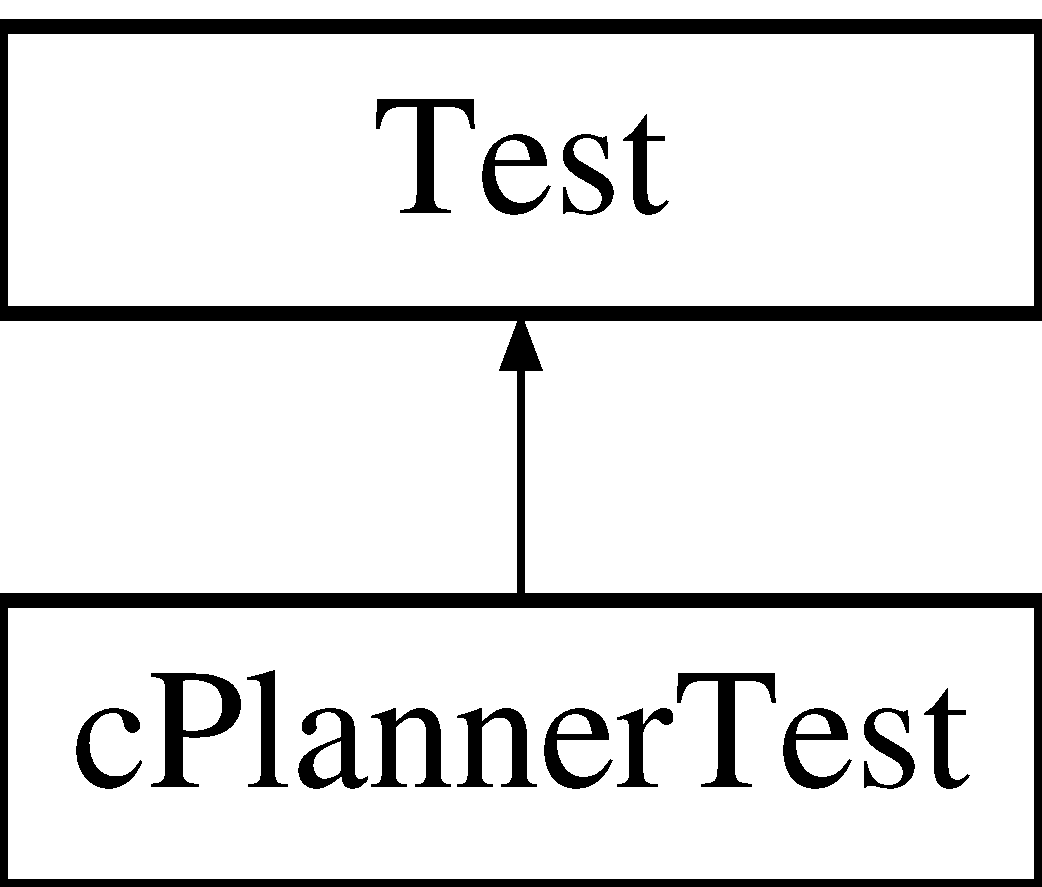
\includegraphics[height=2.000000cm]{classc_planner_test}
\end{center}
\end{figure}
\subsection*{Protected Member Functions}
\begin{DoxyCompactItemize}
\item 
void \mbox{\hyperlink{classc_planner_test_af8a0f625c6cb4dffc1ea3182332e53c6}{Read\+Data}} (std\+::string i\+\_\+str\+Elevation, std\+::string i\+\_\+str\+Overrides)
\item 
\mbox{\Hypertarget{classc_planner_test_ac1aac6152ea3ac86c5205fd8f0835d0c}\label{classc_planner_test_ac1aac6152ea3ac86c5205fd8f0835d0c}} 
void {\bfseries Init\+Island\+Map} ()
\item 
\mbox{\Hypertarget{classc_planner_test_a88ad8b0e63c66a9d94c7606aa67ef20d}\label{classc_planner_test_a88ad8b0e63c66a9d94c7606aa67ef20d}} 
void {\bfseries Set\+Up} () override
\item 
void \mbox{\hyperlink{classc_planner_test_a1e8b184185494cae8444fb7d5f846334}{Create\+Simple\+Map\+With\+Water}} ()
\item 
\mbox{\Hypertarget{classc_planner_test_aa55c78961deacf34543933e12cd82000}\label{classc_planner_test_aa55c78961deacf34543933e12cd82000}} 
void {\bfseries Init\+Simple\+Map\+With\+Water} ()
\item 
void \mbox{\hyperlink{classc_planner_test_a3d08d274ae12fbecd664ec70b4d6dfa3}{Create\+Simple\+Map\+With\+Elevation}} ()
\item 
\mbox{\Hypertarget{classc_planner_test_a59339eef13103205b18ab2f1b1f59d7e}\label{classc_planner_test_a59339eef13103205b18ab2f1b1f59d7e}} 
void {\bfseries Init\+Simple\+Map\+With\+Elevation} ()
\item 
void \mbox{\hyperlink{classc_planner_test_adc6dedb45d227191f0c87843a182d802}{Create\+Rover}} (const t\+Location \&i\+\_\+s\+Start, const t\+Location \&i\+\_\+s\+Goal)
\item 
\mbox{\Hypertarget{classc_planner_test_ae7db6ebf867e3ba6bf8adaaca636f064}\label{classc_planner_test_ae7db6ebf867e3ba6bf8adaaca636f064}} 
void {\bfseries Tear\+Down} () override
\item 
void \mbox{\hyperlink{classc_planner_test_af8a0f625c6cb4dffc1ea3182332e53c6}{Read\+Data}} (std\+::string i\+\_\+str\+Elevation, std\+::string i\+\_\+str\+Overrides)
\item 
\mbox{\Hypertarget{classc_planner_test_ac1aac6152ea3ac86c5205fd8f0835d0c}\label{classc_planner_test_ac1aac6152ea3ac86c5205fd8f0835d0c}} 
void {\bfseries Init\+Island\+Map} ()
\item 
\mbox{\Hypertarget{classc_planner_test_a88ad8b0e63c66a9d94c7606aa67ef20d}\label{classc_planner_test_a88ad8b0e63c66a9d94c7606aa67ef20d}} 
void {\bfseries Set\+Up} () override
\item 
void \mbox{\hyperlink{classc_planner_test_a1e8b184185494cae8444fb7d5f846334}{Create\+Simple\+Map\+With\+Water}} ()
\item 
\mbox{\Hypertarget{classc_planner_test_aa55c78961deacf34543933e12cd82000}\label{classc_planner_test_aa55c78961deacf34543933e12cd82000}} 
void {\bfseries Init\+Simple\+Map\+With\+Water} ()
\item 
void \mbox{\hyperlink{classc_planner_test_a3d08d274ae12fbecd664ec70b4d6dfa3}{Create\+Simple\+Map\+With\+Elevation}} ()
\item 
\mbox{\Hypertarget{classc_planner_test_a59339eef13103205b18ab2f1b1f59d7e}\label{classc_planner_test_a59339eef13103205b18ab2f1b1f59d7e}} 
void {\bfseries Init\+Simple\+Map\+With\+Elevation} ()
\item 
void \mbox{\hyperlink{classc_planner_test_adc6dedb45d227191f0c87843a182d802}{Create\+Rover}} (const t\+Location \&i\+\_\+s\+Start, const t\+Location \&i\+\_\+s\+Goal)
\item 
\mbox{\Hypertarget{classc_planner_test_ae7db6ebf867e3ba6bf8adaaca636f064}\label{classc_planner_test_ae7db6ebf867e3ba6bf8adaaca636f064}} 
void {\bfseries Tear\+Down} () override
\end{DoxyCompactItemize}
\subsection*{Protected Attributes}
\begin{DoxyCompactItemize}
\item 
\mbox{\Hypertarget{classc_planner_test_a2c83ae3b350736b9005788134eb023e2}\label{classc_planner_test_a2c83ae3b350736b9005788134eb023e2}} 
std\+::vector$<$ uint8\+\_\+t $>$ {\bfseries m\+\_\+o\+Elevation}
\item 
\mbox{\Hypertarget{classc_planner_test_a30d78247a35a834582a09a4b9585b28a}\label{classc_planner_test_a30d78247a35a834582a09a4b9585b28a}} 
std\+::vector$<$ uint8\+\_\+t $>$ {\bfseries m\+\_\+o\+Overrides}
\item 
\mbox{\Hypertarget{classc_planner_test_a15fb3c0b9281c70b51654f88799c0c07}\label{classc_planner_test_a15fb3c0b9281c70b51654f88799c0c07}} 
std\+::shared\+\_\+ptr$<$ c\+Audi\+Rover $>$ {\bfseries m\+\_\+po\+Audi\+Rover}
\item 
\mbox{\Hypertarget{classc_planner_test_a1d1e9b95d362b2f8488c988e9f05583b}\label{classc_planner_test_a1d1e9b95d362b2f8488c988e9f05583b}} 
int {\bfseries m\+\_\+n\+Image\+Dim}
\end{DoxyCompactItemize}
\subsection*{Additional Inherited Members}


\subsection{Detailed Description}
The fixture for testing class \mbox{\hyperlink{classc_planner_test}{c\+Planner\+Test}}. 

\subsection{Member Function Documentation}
\mbox{\Hypertarget{classc_planner_test_adc6dedb45d227191f0c87843a182d802}\label{classc_planner_test_adc6dedb45d227191f0c87843a182d802}} 
\index{c\+Planner\+Test@{c\+Planner\+Test}!Create\+Rover@{Create\+Rover}}
\index{Create\+Rover@{Create\+Rover}!c\+Planner\+Test@{c\+Planner\+Test}}
\subsubsection{\texorpdfstring{Create\+Rover()}{CreateRover()}\hspace{0.1cm}{\footnotesize\ttfamily [1/2]}}
{\footnotesize\ttfamily void c\+Planner\+Test\+::\+Create\+Rover (\begin{DoxyParamCaption}\item[{const t\+Location \&}]{i\+\_\+s\+Start,  }\item[{const t\+Location \&}]{i\+\_\+s\+Goal }\end{DoxyParamCaption})\hspace{0.3cm}{\ttfamily [inline]}, {\ttfamily [protected]}}

Create Audi rover

Bachelor calls Audi rover \mbox{\Hypertarget{classc_planner_test_adc6dedb45d227191f0c87843a182d802}\label{classc_planner_test_adc6dedb45d227191f0c87843a182d802}} 
\index{c\+Planner\+Test@{c\+Planner\+Test}!Create\+Rover@{Create\+Rover}}
\index{Create\+Rover@{Create\+Rover}!c\+Planner\+Test@{c\+Planner\+Test}}
\subsubsection{\texorpdfstring{Create\+Rover()}{CreateRover()}\hspace{0.1cm}{\footnotesize\ttfamily [2/2]}}
{\footnotesize\ttfamily void c\+Planner\+Test\+::\+Create\+Rover (\begin{DoxyParamCaption}\item[{const t\+Location \&}]{i\+\_\+s\+Start,  }\item[{const t\+Location \&}]{i\+\_\+s\+Goal }\end{DoxyParamCaption})\hspace{0.3cm}{\ttfamily [inline]}, {\ttfamily [protected]}}

Create Audi rover

Bachelor calls Audi rover \mbox{\Hypertarget{classc_planner_test_a3d08d274ae12fbecd664ec70b4d6dfa3}\label{classc_planner_test_a3d08d274ae12fbecd664ec70b4d6dfa3}} 
\index{c\+Planner\+Test@{c\+Planner\+Test}!Create\+Simple\+Map\+With\+Elevation@{Create\+Simple\+Map\+With\+Elevation}}
\index{Create\+Simple\+Map\+With\+Elevation@{Create\+Simple\+Map\+With\+Elevation}!c\+Planner\+Test@{c\+Planner\+Test}}
\subsubsection{\texorpdfstring{Create\+Simple\+Map\+With\+Elevation()}{CreateSimpleMapWithElevation()}\hspace{0.1cm}{\footnotesize\ttfamily [1/2]}}
{\footnotesize\ttfamily void c\+Planner\+Test\+::\+Create\+Simple\+Map\+With\+Elevation (\begin{DoxyParamCaption}{ }\end{DoxyParamCaption})\hspace{0.3cm}{\ttfamily [inline]}, {\ttfamily [protected]}}

Prepare to read elevation and overrides data \mbox{\Hypertarget{classc_planner_test_a3d08d274ae12fbecd664ec70b4d6dfa3}\label{classc_planner_test_a3d08d274ae12fbecd664ec70b4d6dfa3}} 
\index{c\+Planner\+Test@{c\+Planner\+Test}!Create\+Simple\+Map\+With\+Elevation@{Create\+Simple\+Map\+With\+Elevation}}
\index{Create\+Simple\+Map\+With\+Elevation@{Create\+Simple\+Map\+With\+Elevation}!c\+Planner\+Test@{c\+Planner\+Test}}
\subsubsection{\texorpdfstring{Create\+Simple\+Map\+With\+Elevation()}{CreateSimpleMapWithElevation()}\hspace{0.1cm}{\footnotesize\ttfamily [2/2]}}
{\footnotesize\ttfamily void c\+Planner\+Test\+::\+Create\+Simple\+Map\+With\+Elevation (\begin{DoxyParamCaption}{ }\end{DoxyParamCaption})\hspace{0.3cm}{\ttfamily [inline]}, {\ttfamily [protected]}}

Prepare to read elevation and overrides data \mbox{\Hypertarget{classc_planner_test_a1e8b184185494cae8444fb7d5f846334}\label{classc_planner_test_a1e8b184185494cae8444fb7d5f846334}} 
\index{c\+Planner\+Test@{c\+Planner\+Test}!Create\+Simple\+Map\+With\+Water@{Create\+Simple\+Map\+With\+Water}}
\index{Create\+Simple\+Map\+With\+Water@{Create\+Simple\+Map\+With\+Water}!c\+Planner\+Test@{c\+Planner\+Test}}
\subsubsection{\texorpdfstring{Create\+Simple\+Map\+With\+Water()}{CreateSimpleMapWithWater()}\hspace{0.1cm}{\footnotesize\ttfamily [1/2]}}
{\footnotesize\ttfamily void c\+Planner\+Test\+::\+Create\+Simple\+Map\+With\+Water (\begin{DoxyParamCaption}{ }\end{DoxyParamCaption})\hspace{0.3cm}{\ttfamily [inline]}, {\ttfamily [protected]}}

Prepare to read elevation and overrides data \mbox{\Hypertarget{classc_planner_test_a1e8b184185494cae8444fb7d5f846334}\label{classc_planner_test_a1e8b184185494cae8444fb7d5f846334}} 
\index{c\+Planner\+Test@{c\+Planner\+Test}!Create\+Simple\+Map\+With\+Water@{Create\+Simple\+Map\+With\+Water}}
\index{Create\+Simple\+Map\+With\+Water@{Create\+Simple\+Map\+With\+Water}!c\+Planner\+Test@{c\+Planner\+Test}}
\subsubsection{\texorpdfstring{Create\+Simple\+Map\+With\+Water()}{CreateSimpleMapWithWater()}\hspace{0.1cm}{\footnotesize\ttfamily [2/2]}}
{\footnotesize\ttfamily void c\+Planner\+Test\+::\+Create\+Simple\+Map\+With\+Water (\begin{DoxyParamCaption}{ }\end{DoxyParamCaption})\hspace{0.3cm}{\ttfamily [inline]}, {\ttfamily [protected]}}

Prepare to read elevation and overrides data \mbox{\Hypertarget{classc_planner_test_af8a0f625c6cb4dffc1ea3182332e53c6}\label{classc_planner_test_af8a0f625c6cb4dffc1ea3182332e53c6}} 
\index{c\+Planner\+Test@{c\+Planner\+Test}!Read\+Data@{Read\+Data}}
\index{Read\+Data@{Read\+Data}!c\+Planner\+Test@{c\+Planner\+Test}}
\subsubsection{\texorpdfstring{Read\+Data()}{ReadData()}\hspace{0.1cm}{\footnotesize\ttfamily [1/2]}}
{\footnotesize\ttfamily void c\+Planner\+Test\+::\+Read\+Data (\begin{DoxyParamCaption}\item[{std\+::string}]{i\+\_\+str\+Elevation,  }\item[{std\+::string}]{i\+\_\+str\+Overrides }\end{DoxyParamCaption})\hspace{0.3cm}{\ttfamily [inline]}, {\ttfamily [protected]}}

Prepare to read elevation and overrides data \mbox{\Hypertarget{classc_planner_test_af8a0f625c6cb4dffc1ea3182332e53c6}\label{classc_planner_test_af8a0f625c6cb4dffc1ea3182332e53c6}} 
\index{c\+Planner\+Test@{c\+Planner\+Test}!Read\+Data@{Read\+Data}}
\index{Read\+Data@{Read\+Data}!c\+Planner\+Test@{c\+Planner\+Test}}
\subsubsection{\texorpdfstring{Read\+Data()}{ReadData()}\hspace{0.1cm}{\footnotesize\ttfamily [2/2]}}
{\footnotesize\ttfamily void c\+Planner\+Test\+::\+Read\+Data (\begin{DoxyParamCaption}\item[{std\+::string}]{i\+\_\+str\+Elevation,  }\item[{std\+::string}]{i\+\_\+str\+Overrides }\end{DoxyParamCaption})\hspace{0.3cm}{\ttfamily [inline]}, {\ttfamily [protected]}}

Prepare to read elevation and overrides data 

The documentation for this class was generated from the following file\+:\begin{DoxyCompactItemize}
\item 
/\+Users/fjp/git/bachelor/bachelor-\/master\+\_\+updated\+\_\+vfinal/planner/test/test\+\_\+fixture.\+h\end{DoxyCompactItemize}

\hypertarget{classplanner_1_1c_planner_wiki}{}\section{planner\+:\+:c\+Planner\+Wiki Class Reference}
\label{classplanner_1_1c_planner_wiki}\index{planner\+::c\+Planner\+Wiki@{planner\+::c\+Planner\+Wiki}}


Extends the planner class to implement A$\ast$ from Wikipedia.  




{\ttfamily \#include $<$planner\+\_\+wiki.\+h$>$}

Inheritance diagram for planner\+:\+:c\+Planner\+Wiki\+:\begin{figure}[H]
\begin{center}
\leavevmode
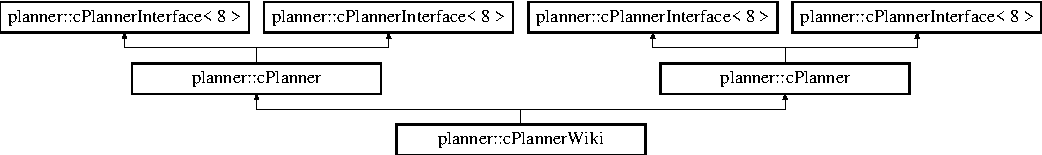
\includegraphics[height=2.089552cm]{classplanner_1_1c_planner_wiki}
\end{center}
\end{figure}
\subsection*{Public Member Functions}
\begin{DoxyCompactItemize}
\item 
\mbox{\hyperlink{classplanner_1_1c_planner_wiki_aed6ae97e85a338e082ec2879629f0f3b}{c\+Planner\+Wiki}} (std\+::shared\+\_\+ptr$<$ \mbox{\hyperlink{classplanner_1_1c_rover_interface}{c\+Rover\+Interface}}$<$ 8 $>$$>$ i\+\_\+po\+Rover, std\+::shared\+\_\+ptr$<$ \mbox{\hyperlink{classplanner_1_1c_graph}{c\+Graph}} $>$ i\+\_\+o\+Map)
\begin{DoxyCompactList}\small\item\em Initializes member variables m\+\_\+po\+Rover and m\+\_\+o\+Map and calls \mbox{\hyperlink{classplanner_1_1c_planner_a2e5a745f83f903662eff914d8beddb5e}{Calculate\+Consistency\+Factor()}}. \end{DoxyCompactList}\item 
\mbox{\Hypertarget{classplanner_1_1c_planner_wiki_ab9f2b825a5b1e0bd2e33271f25c812be}\label{classplanner_1_1c_planner_wiki_ab9f2b825a5b1e0bd2e33271f25c812be}} 
\mbox{\hyperlink{classplanner_1_1c_planner_wiki_ab9f2b825a5b1e0bd2e33271f25c812be}{$\sim$c\+Planner\+Wiki}} ()
\begin{DoxyCompactList}\small\item\em Destructor to delete the allocated memory. \end{DoxyCompactList}\item 
\mbox{\hyperlink{structt_result}{t\+Result}} \mbox{\hyperlink{classplanner_1_1c_planner_wiki_a9d18be721400b51162ff463ab11d1721}{Plan}} () override
\begin{DoxyCompactList}\small\item\em Override of the base interface \mbox{\hyperlink{classplanner_1_1c_planner_interface}{c\+Planner\+Interface}}, which invokes the \mbox{\hyperlink{classplanner_1_1c_planner_wiki_aa673ebc2b1b43af3b13fb0c958c5f2e4}{A\+Star()}} search algorithm. \end{DoxyCompactList}\item 
{\footnotesize template$<$typename T\+Cost\+So\+Far , typename T\+Came\+From $>$ }\\void \mbox{\hyperlink{classplanner_1_1c_planner_wiki_a049e5c4a9540fecbe82a0648f771bbd2}{Reconstruct\+Path}} (T\+Cost\+So\+Far \&\&i\+\_\+cost\+\_\+so\+\_\+far, T\+Came\+From \&\&i\+\_\+came\+\_\+from)
\begin{DoxyCompactList}\small\item\em Given the node i\+\_\+ps\+Node the overrides map m\+\_\+po\+Overrides is updated for displaying the path. \end{DoxyCompactList}\item 
\mbox{\hyperlink{classplanner_1_1c_planner_wiki_aed6ae97e85a338e082ec2879629f0f3b}{c\+Planner\+Wiki}} (std\+::shared\+\_\+ptr$<$ \mbox{\hyperlink{classplanner_1_1c_rover_interface}{c\+Rover\+Interface}}$<$ 8 $>$$>$ i\+\_\+po\+Rover, std\+::shared\+\_\+ptr$<$ \mbox{\hyperlink{classplanner_1_1c_graph}{c\+Graph}} $>$ i\+\_\+o\+Map)
\begin{DoxyCompactList}\small\item\em Initializes member variables m\+\_\+po\+Rover and m\+\_\+o\+Map and calls \mbox{\hyperlink{classplanner_1_1c_planner_a2e5a745f83f903662eff914d8beddb5e}{Calculate\+Consistency\+Factor()}}. \end{DoxyCompactList}\item 
\mbox{\Hypertarget{classplanner_1_1c_planner_wiki_ab9f2b825a5b1e0bd2e33271f25c812be}\label{classplanner_1_1c_planner_wiki_ab9f2b825a5b1e0bd2e33271f25c812be}} 
\mbox{\hyperlink{classplanner_1_1c_planner_wiki_ab9f2b825a5b1e0bd2e33271f25c812be}{$\sim$c\+Planner\+Wiki}} ()
\begin{DoxyCompactList}\small\item\em Destructor to delete the allocated memory. \end{DoxyCompactList}\item 
\mbox{\hyperlink{structt_result}{t\+Result}} \mbox{\hyperlink{classplanner_1_1c_planner_wiki_a9d18be721400b51162ff463ab11d1721}{Plan}} () override
\begin{DoxyCompactList}\small\item\em Override of the base interface \mbox{\hyperlink{classplanner_1_1c_planner_interface}{c\+Planner\+Interface}}, which invokes the \mbox{\hyperlink{classplanner_1_1c_planner_wiki_aa673ebc2b1b43af3b13fb0c958c5f2e4}{A\+Star()}} search algorithm. \end{DoxyCompactList}\item 
{\footnotesize template$<$typename T\+Cost\+So\+Far , typename T\+Came\+From $>$ }\\void \mbox{\hyperlink{classplanner_1_1c_planner_wiki_a049e5c4a9540fecbe82a0648f771bbd2}{Reconstruct\+Path}} (T\+Cost\+So\+Far \&\&i\+\_\+cost\+\_\+so\+\_\+far, T\+Came\+From \&\&i\+\_\+came\+\_\+from)
\begin{DoxyCompactList}\small\item\em Given the node i\+\_\+ps\+Node the overrides map m\+\_\+po\+Overrides is updated for displaying the path. \end{DoxyCompactList}\end{DoxyCompactItemize}
\subsection*{Protected Member Functions}
\begin{DoxyCompactItemize}
\item 
\mbox{\hyperlink{structt_result}{t\+Result}} \mbox{\hyperlink{classplanner_1_1c_planner_wiki_aa673ebc2b1b43af3b13fb0c958c5f2e4}{A\+Star}} ()
\item 
\mbox{\Hypertarget{classplanner_1_1c_planner_wiki_aa673ebc2b1b43af3b13fb0c958c5f2e4}\label{classplanner_1_1c_planner_wiki_aa673ebc2b1b43af3b13fb0c958c5f2e4}} 
\mbox{\hyperlink{structt_result}{t\+Result}} {\bfseries A\+Star} ()
\end{DoxyCompactItemize}
\subsection*{Additional Inherited Members}


\subsection{Detailed Description}
Extends the planner class to implement A$\ast$ from Wikipedia. 

\subsection{Constructor \& Destructor Documentation}
\mbox{\Hypertarget{classplanner_1_1c_planner_wiki_aed6ae97e85a338e082ec2879629f0f3b}\label{classplanner_1_1c_planner_wiki_aed6ae97e85a338e082ec2879629f0f3b}} 
\index{planner\+::c\+Planner\+Wiki@{planner\+::c\+Planner\+Wiki}!c\+Planner\+Wiki@{c\+Planner\+Wiki}}
\index{c\+Planner\+Wiki@{c\+Planner\+Wiki}!planner\+::c\+Planner\+Wiki@{planner\+::c\+Planner\+Wiki}}
\subsubsection{\texorpdfstring{c\+Planner\+Wiki()}{cPlannerWiki()}\hspace{0.1cm}{\footnotesize\ttfamily [1/2]}}
{\footnotesize\ttfamily planner\+::c\+Planner\+Wiki\+::c\+Planner\+Wiki (\begin{DoxyParamCaption}\item[{std\+::shared\+\_\+ptr$<$ \mbox{\hyperlink{classplanner_1_1c_rover_interface}{c\+Rover\+Interface}}$<$ 8 $>$$>$}]{i\+\_\+po\+Rover,  }\item[{std\+::shared\+\_\+ptr$<$ \mbox{\hyperlink{classplanner_1_1c_graph}{c\+Graph}} $>$}]{i\+\_\+o\+Map }\end{DoxyParamCaption})}



Initializes member variables m\+\_\+po\+Rover and m\+\_\+o\+Map and calls \mbox{\hyperlink{classplanner_1_1c_planner_a2e5a745f83f903662eff914d8beddb5e}{Calculate\+Consistency\+Factor()}}. 

The \mbox{\Hypertarget{classplanner_1_1c_planner_wiki_aed6ae97e85a338e082ec2879629f0f3b}\label{classplanner_1_1c_planner_wiki_aed6ae97e85a338e082ec2879629f0f3b}} 
\index{planner\+::c\+Planner\+Wiki@{planner\+::c\+Planner\+Wiki}!c\+Planner\+Wiki@{c\+Planner\+Wiki}}
\index{c\+Planner\+Wiki@{c\+Planner\+Wiki}!planner\+::c\+Planner\+Wiki@{planner\+::c\+Planner\+Wiki}}
\subsubsection{\texorpdfstring{c\+Planner\+Wiki()}{cPlannerWiki()}\hspace{0.1cm}{\footnotesize\ttfamily [2/2]}}
{\footnotesize\ttfamily planner\+::c\+Planner\+Wiki\+::c\+Planner\+Wiki (\begin{DoxyParamCaption}\item[{std\+::shared\+\_\+ptr$<$ \mbox{\hyperlink{classplanner_1_1c_rover_interface}{c\+Rover\+Interface}}$<$ 8 $>$$>$}]{i\+\_\+po\+Rover,  }\item[{std\+::shared\+\_\+ptr$<$ \mbox{\hyperlink{classplanner_1_1c_graph}{c\+Graph}} $>$}]{i\+\_\+o\+Map }\end{DoxyParamCaption})}



Initializes member variables m\+\_\+po\+Rover and m\+\_\+o\+Map and calls \mbox{\hyperlink{classplanner_1_1c_planner_a2e5a745f83f903662eff914d8beddb5e}{Calculate\+Consistency\+Factor()}}. 

The 

\subsection{Member Function Documentation}
\mbox{\Hypertarget{classplanner_1_1c_planner_wiki_aa673ebc2b1b43af3b13fb0c958c5f2e4}\label{classplanner_1_1c_planner_wiki_aa673ebc2b1b43af3b13fb0c958c5f2e4}} 
\index{planner\+::c\+Planner\+Wiki@{planner\+::c\+Planner\+Wiki}!A\+Star@{A\+Star}}
\index{A\+Star@{A\+Star}!planner\+::c\+Planner\+Wiki@{planner\+::c\+Planner\+Wiki}}
\subsubsection{\texorpdfstring{A\+Star()}{AStar()}}
{\footnotesize\ttfamily \mbox{\hyperlink{structt_result}{t\+Result}} planner\+::c\+Planner\+Wiki\+::\+A\+Star (\begin{DoxyParamCaption}{ }\end{DoxyParamCaption})\hspace{0.3cm}{\ttfamily [protected]}}

The set of nodes already evaluated. Implemented as 2d array filled with 0s and start element set to 1.

The set of currently discovered nodes that are not evaluated yet. Initially, only the start node is known. ~\newline
~\newline
~\newline
~\newline
~\newline
~\newline
~\newline
~\newline
~\newline
~\newline
~\newline
~\newline
~\newline
~\newline
~\newline
~\newline
 Defined the simplified start node

For each node, which action it can most efficiently be reached from. If a node can be reached from many nodes, action will eventually contain the most efficient previous step. ~\newline
~\newline
~\newline
~\newline
~\newline
~\newline
~\newline
~\newline
~\newline
~\newline
~\newline
~\newline
~\newline
~\newline
 For each node, the cost of getting from the start node to that node.

The cost of going from start to start is zero.

Initialize result struct

While the goal is not found the problem is solvable

Resign if no values in the open list and you can\textquotesingle{}t expand anymore

Remove the node from the open priority queue having the lowest f\+Score value

Check if the goal is reached

Otherwise explore new locations

Add the current node to the set of nodes already evaluated

Perform each possible rover action on the current node

Check if the location of the next node lies within the map and is not on water. Ignore the neighbors which are already evaluated (closed\mbox{[}n\+X\+Next\mbox{]}\mbox{[}n\+Y\+Next\mbox{]} == 0). ~\newline
~\newline
~\newline
 The distance from start to a neighbor

Mark visited nodes

Check that heuristic never overestimates the true distance\+: Priority of a new node should never be lower than the priority of its parent.

The set of nodes already evaluated. Implemented as 2d array filled with 0s and start element set to 1.

The set of currently discovered nodes that are not evaluated yet. Initially, only the start node is known. ~\newline
~\newline
~\newline
~\newline
~\newline
~\newline
~\newline
~\newline
~\newline
~\newline
~\newline
~\newline
~\newline
~\newline
~\newline
~\newline
~\newline
 Defined the simplified start node

For each node, which action it can most efficiently be reached from. If a node can be reached from many nodes, action will eventually contain the most efficient previous step. ~\newline
~\newline
~\newline
~\newline
~\newline
~\newline
~\newline
~\newline
~\newline
~\newline
~\newline
~\newline
~\newline
~\newline
~\newline
 For each node, the cost of getting from the start node to that node.

The cost of going from start to start is zero.

Initialize result struct

While the goal is not found the problem is solvable

Resign if no values in the open list and you can\textquotesingle{}t expand anymore

Remove the node from the open priority queue having the lowest f\+Score value

Check if the goal is reached

Otherwise explore new locations

Add the current node to the set of nodes already evaluated

Perform each possible rover action on the current node

Check if the location of the next node lies within the map and is not on water. Ignore the neighbors which are already evaluated (closed\mbox{[}n\+X\+Next\mbox{]}\mbox{[}n\+Y\+Next\mbox{]} == 0). ~\newline
~\newline
~\newline
~\newline
 The distance from start to a neighbor

Mark visited nodes

Check that heuristic never overestimates the true distance\+: Priority of a new node should never be lower than the priority of its parent. ~\newline
 Move from the current node back to the start node \mbox{\Hypertarget{classplanner_1_1c_planner_wiki_a9d18be721400b51162ff463ab11d1721}\label{classplanner_1_1c_planner_wiki_a9d18be721400b51162ff463ab11d1721}} 
\index{planner\+::c\+Planner\+Wiki@{planner\+::c\+Planner\+Wiki}!Plan@{Plan}}
\index{Plan@{Plan}!planner\+::c\+Planner\+Wiki@{planner\+::c\+Planner\+Wiki}}
\subsubsection{\texorpdfstring{Plan()}{Plan()}\hspace{0.1cm}{\footnotesize\ttfamily [1/2]}}
{\footnotesize\ttfamily \mbox{\hyperlink{structt_result}{t\+Result}} planner\+::c\+Planner\+Wiki\+::\+Plan (\begin{DoxyParamCaption}{ }\end{DoxyParamCaption})\hspace{0.3cm}{\ttfamily [override]}, {\ttfamily [virtual]}}



Override of the base interface \mbox{\hyperlink{classplanner_1_1c_planner_interface}{c\+Planner\+Interface}}, which invokes the \mbox{\hyperlink{classplanner_1_1c_planner_wiki_aa673ebc2b1b43af3b13fb0c958c5f2e4}{A\+Star()}} search algorithm. 

\begin{DoxyReturn}{Returns}
the time to travel from start to goal if it was found. Otherwise -\/1 is returned. 
\end{DoxyReturn}


Reimplemented from \mbox{\hyperlink{classplanner_1_1c_planner_a21230c015260b9fc34ad2f239592470e}{planner\+::c\+Planner}}.

\mbox{\Hypertarget{classplanner_1_1c_planner_wiki_a9d18be721400b51162ff463ab11d1721}\label{classplanner_1_1c_planner_wiki_a9d18be721400b51162ff463ab11d1721}} 
\index{planner\+::c\+Planner\+Wiki@{planner\+::c\+Planner\+Wiki}!Plan@{Plan}}
\index{Plan@{Plan}!planner\+::c\+Planner\+Wiki@{planner\+::c\+Planner\+Wiki}}
\subsubsection{\texorpdfstring{Plan()}{Plan()}\hspace{0.1cm}{\footnotesize\ttfamily [2/2]}}
{\footnotesize\ttfamily \mbox{\hyperlink{structt_result}{t\+Result}} planner\+::c\+Planner\+Wiki\+::\+Plan (\begin{DoxyParamCaption}{ }\end{DoxyParamCaption})\hspace{0.3cm}{\ttfamily [override]}, {\ttfamily [virtual]}}



Override of the base interface \mbox{\hyperlink{classplanner_1_1c_planner_interface}{c\+Planner\+Interface}}, which invokes the \mbox{\hyperlink{classplanner_1_1c_planner_wiki_aa673ebc2b1b43af3b13fb0c958c5f2e4}{A\+Star()}} search algorithm. 

\begin{DoxyReturn}{Returns}
the time to travel from start to goal if it was found. Otherwise -\/1 is returned. 
\end{DoxyReturn}


Reimplemented from \mbox{\hyperlink{classplanner_1_1c_planner_a21230c015260b9fc34ad2f239592470e}{planner\+::c\+Planner}}.

\mbox{\Hypertarget{classplanner_1_1c_planner_wiki_a049e5c4a9540fecbe82a0648f771bbd2}\label{classplanner_1_1c_planner_wiki_a049e5c4a9540fecbe82a0648f771bbd2}} 
\index{planner\+::c\+Planner\+Wiki@{planner\+::c\+Planner\+Wiki}!Reconstruct\+Path@{Reconstruct\+Path}}
\index{Reconstruct\+Path@{Reconstruct\+Path}!planner\+::c\+Planner\+Wiki@{planner\+::c\+Planner\+Wiki}}
\subsubsection{\texorpdfstring{Reconstruct\+Path()}{ReconstructPath()}\hspace{0.1cm}{\footnotesize\ttfamily [1/2]}}
{\footnotesize\ttfamily template$<$typename T\+Cost\+So\+Far , typename T\+Came\+From $>$ \\
void planner\+::c\+Planner\+Wiki\+::\+Reconstruct\+Path (\begin{DoxyParamCaption}\item[{T\+Cost\+So\+Far \&\&}]{i\+\_\+cost\+\_\+so\+\_\+far,  }\item[{T\+Came\+From \&\&}]{i\+\_\+came\+\_\+from }\end{DoxyParamCaption})}



Given the node i\+\_\+ps\+Node the overrides map m\+\_\+po\+Overrides is updated for displaying the path. 

Traversing a path takes place using the m\+\_\+ps\+Parent field of the \mbox{\hyperlink{structplanner_1_1t_node}{t\+Node}} struct. 
\begin{DoxyParams}[1]{Parameters}
\mbox{\tt in}  & {\em i\+\_\+ps\+Node} & Goal node or any other which is traversed back \\
\hline
\end{DoxyParams}
Set the cost (time) it takes to get to the goal

Reconstruct the path by going backward

Update cumulative elevation

Store path in overrides

Check if the current node is the start node

Move towards the start

Update cumulative elevation

Store path in overrides

Set the cost (time) it takes to get to the goal

Reconstruct the path by going backward

Update cumulative elevation

Store path in overrides

Check if the current node is the start node

Move towards the start

Update cumulative elevation

Store path in overrides \mbox{\Hypertarget{classplanner_1_1c_planner_wiki_a049e5c4a9540fecbe82a0648f771bbd2}\label{classplanner_1_1c_planner_wiki_a049e5c4a9540fecbe82a0648f771bbd2}} 
\index{planner\+::c\+Planner\+Wiki@{planner\+::c\+Planner\+Wiki}!Reconstruct\+Path@{Reconstruct\+Path}}
\index{Reconstruct\+Path@{Reconstruct\+Path}!planner\+::c\+Planner\+Wiki@{planner\+::c\+Planner\+Wiki}}
\subsubsection{\texorpdfstring{Reconstruct\+Path()}{ReconstructPath()}\hspace{0.1cm}{\footnotesize\ttfamily [2/2]}}
{\footnotesize\ttfamily template$<$typename T\+Cost\+So\+Far , typename T\+Came\+From $>$ \\
void planner\+::c\+Planner\+Wiki\+::\+Reconstruct\+Path (\begin{DoxyParamCaption}\item[{T\+Cost\+So\+Far \&\&}]{i\+\_\+cost\+\_\+so\+\_\+far,  }\item[{T\+Came\+From \&\&}]{i\+\_\+came\+\_\+from }\end{DoxyParamCaption})}



Given the node i\+\_\+ps\+Node the overrides map m\+\_\+po\+Overrides is updated for displaying the path. 

Traversing a path takes place using the m\+\_\+ps\+Parent field of the \mbox{\hyperlink{structplanner_1_1t_node}{t\+Node}} struct. 
\begin{DoxyParams}[1]{Parameters}
\mbox{\tt in}  & {\em i\+\_\+ps\+Node} & Goal node or any other which is traversed back \\
\hline
\end{DoxyParams}


The documentation for this class was generated from the following files\+:\begin{DoxyCompactItemize}
\item 
/\+Users/fjp/git/bachelor/bachelor-\/master\+\_\+updated\+\_\+vfinal/planner/include/planner\+\_\+wiki.\+h\item 
/\+Users/fjp/git/bachelor/bachelor-\/master\+\_\+updated\+\_\+vfinal/planner/src/planner\+\_\+wiki.\+cpp\end{DoxyCompactItemize}

\hypertarget{classplanner_1_1c_rover_interface}{}\section{planner\+:\+:c\+Rover\+Interface$<$ Directions $>$ Class Template Reference}
\label{classplanner_1_1c_rover_interface}\index{planner\+::c\+Rover\+Interface$<$ Directions $>$@{planner\+::c\+Rover\+Interface$<$ Directions $>$}}


Forward declaration of interface \mbox{\hyperlink{classplanner_1_1c_rover_interface}{planner\+::c\+Rover\+Interface}}.  




{\ttfamily \#include $<$planner\+\_\+interface.\+h$>$}



Collaboration diagram for planner\+:\+:c\+Rover\+Interface$<$ Directions $>$\+:
\nopagebreak
\begin{figure}[H]
\begin{center}
\leavevmode
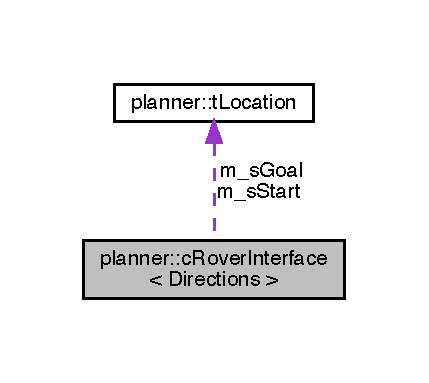
\includegraphics[width=206pt]{classplanner_1_1c_rover_interface__coll__graph}
\end{center}
\end{figure}
\subsection*{Public Member Functions}
\begin{DoxyCompactItemize}
\item 
\mbox{\Hypertarget{classplanner_1_1c_rover_interface_a7fedea18832ad850de1a2589fdca88b7}\label{classplanner_1_1c_rover_interface_a7fedea18832ad850de1a2589fdca88b7}} 
virtual std\+::shared\+\_\+ptr$<$ \mbox{\hyperlink{classplanner_1_1c_planner_interface}{c\+Planner\+Interface}}$<$ Directions $>$ $>$ {\bfseries Initialize\+Planner} (const int \&i\+\_\+n\+Step\+Size, const int \&i\+\_\+n\+Velocity, std\+::string \&\&i\+\_\+str\+Algorithm)=0
\item 
\mbox{\Hypertarget{classplanner_1_1c_rover_interface_ad2b552aaf43f7ce5af340d05b5657267}\label{classplanner_1_1c_rover_interface_ad2b552aaf43f7ce5af340d05b5657267}} 
double \mbox{\hyperlink{classplanner_1_1c_rover_interface_ad2b552aaf43f7ce5af340d05b5657267}{Cost\+Straight}} () const
\begin{DoxyCompactList}\small\item\em Getter and Setter for the private member varialbes. \end{DoxyCompactList}\item 
\mbox{\Hypertarget{classplanner_1_1c_rover_interface_ab4c45b0f0c586f864a83ba90be06efd0}\label{classplanner_1_1c_rover_interface_ab4c45b0f0c586f864a83ba90be06efd0}} 
double {\bfseries Cost\+Diagonal} () const
\item 
\mbox{\Hypertarget{classplanner_1_1c_rover_interface_ac2f57f4b9bf2c01fbcf1ca3c6d1fc55d}\label{classplanner_1_1c_rover_interface_ac2f57f4b9bf2c01fbcf1ca3c6d1fc55d}} 
void {\bfseries Set\+Cost\+Straight} (double i\+\_\+f\+Cost\+Straight)
\item 
\mbox{\Hypertarget{classplanner_1_1c_rover_interface_a3aa2779928912477dcf76c7767ea746d}\label{classplanner_1_1c_rover_interface_a3aa2779928912477dcf76c7767ea746d}} 
void {\bfseries Set\+Cost\+Diagonal} (double i\+\_\+f\+Cost\+Diagonal)
\item 
\mbox{\Hypertarget{classplanner_1_1c_rover_interface_ad62c6dcbe7c8194c6a93ca1fc29ee4b8}\label{classplanner_1_1c_rover_interface_ad62c6dcbe7c8194c6a93ca1fc29ee4b8}} 
\mbox{\hyperlink{structplanner_1_1t_location}{t\+Location}} \& {\bfseries Start} ()
\item 
\mbox{\Hypertarget{classplanner_1_1c_rover_interface_a29669ceb2b1f4cebf0953b59e3c8936a}\label{classplanner_1_1c_rover_interface_a29669ceb2b1f4cebf0953b59e3c8936a}} 
void {\bfseries Set\+Start} (const \mbox{\hyperlink{structplanner_1_1t_location}{t\+Location}} \&i\+\_\+s\+Start)
\item 
\mbox{\Hypertarget{classplanner_1_1c_rover_interface_a5a02ffb5e04d128bf81567da55807850}\label{classplanner_1_1c_rover_interface_a5a02ffb5e04d128bf81567da55807850}} 
\mbox{\hyperlink{structplanner_1_1t_location}{t\+Location}} \& {\bfseries Goal} ()
\item 
\mbox{\Hypertarget{classplanner_1_1c_rover_interface_a8f0e30cf351e8cb7ba75622273056343}\label{classplanner_1_1c_rover_interface_a8f0e30cf351e8cb7ba75622273056343}} 
void {\bfseries Set\+Goal} (const \mbox{\hyperlink{structplanner_1_1t_location}{t\+Location}} \&i\+\_\+s\+Goal)
\item 
\mbox{\Hypertarget{classplanner_1_1c_rover_interface_a2a10c0d42c89adefa46390fe351583a2}\label{classplanner_1_1c_rover_interface_a2a10c0d42c89adefa46390fe351583a2}} 
int {\bfseries Step\+Size} () const
\item 
\mbox{\Hypertarget{classplanner_1_1c_rover_interface_ac6410b636f0f2d5614e3463912f9646f}\label{classplanner_1_1c_rover_interface_ac6410b636f0f2d5614e3463912f9646f}} 
void {\bfseries Set\+Step\+Size} (int i\+\_\+n\+Step\+Size)
\item 
\mbox{\Hypertarget{classplanner_1_1c_rover_interface_a65279be04ab88f54d69204087503448b}\label{classplanner_1_1c_rover_interface_a65279be04ab88f54d69204087503448b}} 
int {\bfseries Velocity} () const
\item 
\mbox{\Hypertarget{classplanner_1_1c_rover_interface_a209a069d48223e427e27e4582037b158}\label{classplanner_1_1c_rover_interface_a209a069d48223e427e27e4582037b158}} 
void {\bfseries Set\+Velocity} (int i\+\_\+n\+Velocity)
\item 
\mbox{\Hypertarget{classplanner_1_1c_rover_interface_aeab2cd88b65b86f42cfbb5b063d3f9d1}\label{classplanner_1_1c_rover_interface_aeab2cd88b65b86f42cfbb5b063d3f9d1}} 
std\+::shared\+\_\+ptr$<$ \mbox{\hyperlink{classplanner_1_1c_planner_interface}{c\+Planner\+Interface}}$<$ Directions $>$ $>$ {\bfseries Get\+Planner} () const
\end{DoxyCompactItemize}
\subsection*{Public Attributes}
\begin{DoxyCompactItemize}
\item 
\mbox{\Hypertarget{classplanner_1_1c_rover_interface_a119c31cfd1e6aa72921fc5185e6f44a5}\label{classplanner_1_1c_rover_interface_a119c31cfd1e6aa72921fc5185e6f44a5}} 
std\+::array$<$ \mbox{\hyperlink{structplanner_1_1t_action}{t\+Action}}, Directions $>$ \mbox{\hyperlink{classplanner_1_1c_rover_interface_a119c31cfd1e6aa72921fc5185e6f44a5}{m\+\_\+as\+Actions}}
\begin{DoxyCompactList}\small\item\em Array that contains the number of actions in which the robot can move. It has a template size parameter Directions. \end{DoxyCompactList}\end{DoxyCompactItemize}
\subsection*{Protected Attributes}
\begin{DoxyCompactItemize}
\item 
std\+::weak\+\_\+ptr$<$ \mbox{\hyperlink{classplanner_1_1c_planner_interface}{c\+Planner\+Interface}}$<$ Directions $>$ $>$ \mbox{\hyperlink{classplanner_1_1c_rover_interface_a22d4f0d40dd064d62ed75da9728601ea}{m\+\_\+po\+Planner}}
\begin{DoxyCompactList}\small\item\em Pointer to an abstract planner interface. \end{DoxyCompactList}\item 
\mbox{\Hypertarget{classplanner_1_1c_rover_interface_a42552f6e5f1f2909821eaef8535a9979}\label{classplanner_1_1c_rover_interface_a42552f6e5f1f2909821eaef8535a9979}} 
\mbox{\hyperlink{structplanner_1_1t_location}{t\+Location}} \mbox{\hyperlink{classplanner_1_1c_rover_interface_a42552f6e5f1f2909821eaef8535a9979}{m\+\_\+s\+Start}}
\begin{DoxyCompactList}\small\item\em Start location (x,y) of the rover. \end{DoxyCompactList}\item 
\mbox{\Hypertarget{classplanner_1_1c_rover_interface_a705221124f88ca9dbdf706869ebfc96a}\label{classplanner_1_1c_rover_interface_a705221124f88ca9dbdf706869ebfc96a}} 
\mbox{\hyperlink{structplanner_1_1t_location}{t\+Location}} \mbox{\hyperlink{classplanner_1_1c_rover_interface_a705221124f88ca9dbdf706869ebfc96a}{m\+\_\+s\+Goal}}
\begin{DoxyCompactList}\small\item\em Goal location (x,y) of the rover. \end{DoxyCompactList}\item 
\mbox{\Hypertarget{classplanner_1_1c_rover_interface_aea86540c3962e223de84f28ff067d788}\label{classplanner_1_1c_rover_interface_aea86540c3962e223de84f28ff067d788}} 
int \mbox{\hyperlink{classplanner_1_1c_rover_interface_aea86540c3962e223de84f28ff067d788}{m\+\_\+n\+Step\+Size}}
\begin{DoxyCompactList}\small\item\em Step size of the rover, varied to get to the goal quicker. \end{DoxyCompactList}\item 
\mbox{\Hypertarget{classplanner_1_1c_rover_interface_a458f3e469a13cfc909e957678ddee753}\label{classplanner_1_1c_rover_interface_a458f3e469a13cfc909e957678ddee753}} 
int \mbox{\hyperlink{classplanner_1_1c_rover_interface_a458f3e469a13cfc909e957678ddee753}{m\+\_\+n\+Velocity}}
\begin{DoxyCompactList}\small\item\em Speed of the rover (always set to one, not tested). \end{DoxyCompactList}\item 
\mbox{\Hypertarget{classplanner_1_1c_rover_interface_ad94337c2b05eed20423c1a2dcaa680cc}\label{classplanner_1_1c_rover_interface_ad94337c2b05eed20423c1a2dcaa680cc}} 
double \mbox{\hyperlink{classplanner_1_1c_rover_interface_ad94337c2b05eed20423c1a2dcaa680cc}{m\+\_\+f\+Cost\+Straight}}
\begin{DoxyCompactList}\small\item\em Cost to move straight. \end{DoxyCompactList}\item 
\mbox{\Hypertarget{classplanner_1_1c_rover_interface_afcc4b7ec327b8d2ddcdb163c7a8397b3}\label{classplanner_1_1c_rover_interface_afcc4b7ec327b8d2ddcdb163c7a8397b3}} 
double \mbox{\hyperlink{classplanner_1_1c_rover_interface_afcc4b7ec327b8d2ddcdb163c7a8397b3}{m\+\_\+f\+Cost\+Diagonal}}
\begin{DoxyCompactList}\small\item\em Cost to move diagonal. \end{DoxyCompactList}\end{DoxyCompactItemize}


\subsection{Detailed Description}
\subsubsection*{template$<$size\+\_\+t Directions$>$\newline
class planner\+::c\+Rover\+Interface$<$ Directions $>$}

Forward declaration of interface \mbox{\hyperlink{classplanner_1_1c_rover_interface}{planner\+::c\+Rover\+Interface}}. 

\subsection{Member Data Documentation}
\mbox{\Hypertarget{classplanner_1_1c_rover_interface_a22d4f0d40dd064d62ed75da9728601ea}\label{classplanner_1_1c_rover_interface_a22d4f0d40dd064d62ed75da9728601ea}} 
\index{planner\+::c\+Rover\+Interface@{planner\+::c\+Rover\+Interface}!m\+\_\+po\+Planner@{m\+\_\+po\+Planner}}
\index{m\+\_\+po\+Planner@{m\+\_\+po\+Planner}!planner\+::c\+Rover\+Interface@{planner\+::c\+Rover\+Interface}}
\subsubsection{\texorpdfstring{m\+\_\+po\+Planner}{m\_poPlanner}}
{\footnotesize\ttfamily template$<$size\+\_\+t Directions$>$ \\
std\+::weak\+\_\+ptr$<$\mbox{\hyperlink{classplanner_1_1c_planner_interface}{c\+Planner\+Interface}}$<$Directions$>$ $>$ \mbox{\hyperlink{classplanner_1_1c_rover_interface}{planner\+::c\+Rover\+Interface}}$<$ Directions $>$\+::m\+\_\+po\+Planner\hspace{0.3cm}{\ttfamily [protected]}}



Pointer to an abstract planner interface. 

An implementation of this interface should initialize m\+\_\+po\+Planner. 

The documentation for this class was generated from the following files\+:\begin{DoxyCompactItemize}
\item 
/\+Users/fjp/git/bachelor/planner/include/planner\+\_\+interface.\+h\item 
/\+Users/fjp/git/bachelor/planner/include/rover\+\_\+interface.\+h\end{DoxyCompactItemize}

\hypertarget{classtesting_1_1_current_test_info_test}{}\section{testing\+:\+:Current\+Test\+Info\+Test Class Reference}
\label{classtesting_1_1_current_test_info_test}\index{testing\+::\+Current\+Test\+Info\+Test@{testing\+::\+Current\+Test\+Info\+Test}}
Inheritance diagram for testing\+:\+:Current\+Test\+Info\+Test\+:\begin{figure}[H]
\begin{center}
\leavevmode
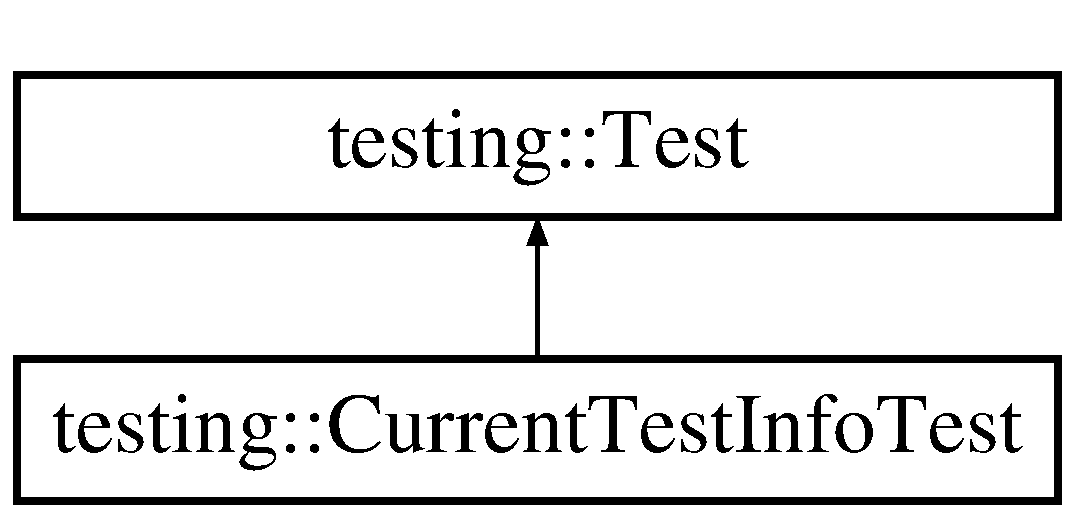
\includegraphics[height=2.000000cm]{classtesting_1_1_current_test_info_test}
\end{center}
\end{figure}
\subsection*{Static Protected Member Functions}
\begin{DoxyCompactItemize}
\item 
\mbox{\Hypertarget{classtesting_1_1_current_test_info_test_a61bad7ce29923afd464daf9684b6269e}\label{classtesting_1_1_current_test_info_test_a61bad7ce29923afd464daf9684b6269e}} 
static void {\bfseries Set\+Up\+Test\+Case} ()
\item 
\mbox{\Hypertarget{classtesting_1_1_current_test_info_test_a9a80a5a3e6e70c619870c2ae9df892a6}\label{classtesting_1_1_current_test_info_test_a9a80a5a3e6e70c619870c2ae9df892a6}} 
static void {\bfseries Tear\+Down\+Test\+Case} ()
\end{DoxyCompactItemize}
\subsection*{Additional Inherited Members}


The documentation for this class was generated from the following file\+:\begin{DoxyCompactItemize}
\item 
/\+Users/fjp/git/bachelor/bachelor-\/master\+\_\+updated\+\_\+vfinal/googletest-\/1.\+8.\+0/googletest/test/gtest\+\_\+unittest.\+cc\end{DoxyCompactItemize}

\hypertarget{classpump_1_1_cursor}{}\section{pump.\+Cursor Class Reference}
\label{classpump_1_1_cursor}\index{pump.\+Cursor@{pump.\+Cursor}}
\subsection*{Public Member Functions}
\begin{DoxyCompactItemize}
\item 
\mbox{\Hypertarget{classpump_1_1_cursor_a17126ae70ca573c43e4d38b1ccd03015}\label{classpump_1_1_cursor_a17126ae70ca573c43e4d38b1ccd03015}} 
def {\bfseries \+\_\+\+\_\+init\+\_\+\+\_\+} (self, line=-\/1, column=-\/1)
\item 
\mbox{\Hypertarget{classpump_1_1_cursor_ab430cfd4cfd2fa2b57ea31b128e56f22}\label{classpump_1_1_cursor_ab430cfd4cfd2fa2b57ea31b128e56f22}} 
def {\bfseries \+\_\+\+\_\+eq\+\_\+\+\_\+} (self, rhs)
\item 
\mbox{\Hypertarget{classpump_1_1_cursor_a7bcfe24fa4e5df6ed12f627b8d3b3ba3}\label{classpump_1_1_cursor_a7bcfe24fa4e5df6ed12f627b8d3b3ba3}} 
def {\bfseries \+\_\+\+\_\+ne\+\_\+\+\_\+} (self, rhs)
\item 
\mbox{\Hypertarget{classpump_1_1_cursor_a4f846e3cf80aa45853b1fb7a03863745}\label{classpump_1_1_cursor_a4f846e3cf80aa45853b1fb7a03863745}} 
def {\bfseries \+\_\+\+\_\+lt\+\_\+\+\_\+} (self, rhs)
\item 
\mbox{\Hypertarget{classpump_1_1_cursor_a7652488b46ecf1dfa4d0a83bff9411ab}\label{classpump_1_1_cursor_a7652488b46ecf1dfa4d0a83bff9411ab}} 
def {\bfseries \+\_\+\+\_\+le\+\_\+\+\_\+} (self, rhs)
\item 
\mbox{\Hypertarget{classpump_1_1_cursor_aa6109b9e7048e6260c2018a6d8878739}\label{classpump_1_1_cursor_aa6109b9e7048e6260c2018a6d8878739}} 
def {\bfseries \+\_\+\+\_\+gt\+\_\+\+\_\+} (self, rhs)
\item 
\mbox{\Hypertarget{classpump_1_1_cursor_aeadc1924f4435a1a67fada88b0bce40a}\label{classpump_1_1_cursor_aeadc1924f4435a1a67fada88b0bce40a}} 
def {\bfseries \+\_\+\+\_\+ge\+\_\+\+\_\+} (self, rhs)
\item 
\mbox{\Hypertarget{classpump_1_1_cursor_ada8d922763be27a0b1745e94748de2c3}\label{classpump_1_1_cursor_ada8d922763be27a0b1745e94748de2c3}} 
def {\bfseries \+\_\+\+\_\+str\+\_\+\+\_\+} (self)
\item 
\mbox{\Hypertarget{classpump_1_1_cursor_a75b9a3cf0d49413437c8d4fc0d1d5ff3}\label{classpump_1_1_cursor_a75b9a3cf0d49413437c8d4fc0d1d5ff3}} 
def {\bfseries \+\_\+\+\_\+add\+\_\+\+\_\+} (self, offset)
\item 
\mbox{\Hypertarget{classpump_1_1_cursor_a297cc8271af2aade66acb5fa5973a748}\label{classpump_1_1_cursor_a297cc8271af2aade66acb5fa5973a748}} 
def {\bfseries \+\_\+\+\_\+sub\+\_\+\+\_\+} (self, offset)
\item 
def \mbox{\hyperlink{classpump_1_1_cursor_af68c9be83b0af87db441b21bc6ce8114}{Clone}} (self)
\end{DoxyCompactItemize}
\subsection*{Public Attributes}
\begin{DoxyCompactItemize}
\item 
\mbox{\Hypertarget{classpump_1_1_cursor_aee8d8b67360da7fc4e635540cb41d48c}\label{classpump_1_1_cursor_aee8d8b67360da7fc4e635540cb41d48c}} 
{\bfseries line}
\item 
\mbox{\Hypertarget{classpump_1_1_cursor_ae73db76c3a845a82afb334633864254e}\label{classpump_1_1_cursor_ae73db76c3a845a82afb334633864254e}} 
{\bfseries column}
\end{DoxyCompactItemize}


\subsection{Detailed Description}
\begin{DoxyVerb}Represents a position (line and column) in a text file.\end{DoxyVerb}
 

\subsection{Member Function Documentation}
\mbox{\Hypertarget{classpump_1_1_cursor_af68c9be83b0af87db441b21bc6ce8114}\label{classpump_1_1_cursor_af68c9be83b0af87db441b21bc6ce8114}} 
\index{pump\+::\+Cursor@{pump\+::\+Cursor}!Clone@{Clone}}
\index{Clone@{Clone}!pump\+::\+Cursor@{pump\+::\+Cursor}}
\subsubsection{\texorpdfstring{Clone()}{Clone()}}
{\footnotesize\ttfamily def pump.\+Cursor.\+Clone (\begin{DoxyParamCaption}\item[{}]{self }\end{DoxyParamCaption})}

\begin{DoxyVerb}Returns a copy of self.\end{DoxyVerb}
 

The documentation for this class was generated from the following file\+:\begin{DoxyCompactItemize}
\item 
/\+Users/fjp/git/bachelor/bachelor-\/master\+\_\+updated\+\_\+vfinal/googletest-\/1.\+8.\+0/googletest/scripts/pump.\+py\end{DoxyCompactItemize}

\hypertarget{classtesting_1_1internal_1_1_default_global_test_part_result_reporter}{}\section{testing\+:\+:internal\+:\+:Default\+Global\+Test\+Part\+Result\+Reporter Class Reference}
\label{classtesting_1_1internal_1_1_default_global_test_part_result_reporter}\index{testing\+::internal\+::\+Default\+Global\+Test\+Part\+Result\+Reporter@{testing\+::internal\+::\+Default\+Global\+Test\+Part\+Result\+Reporter}}
Inheritance diagram for testing\+:\+:internal\+:\+:Default\+Global\+Test\+Part\+Result\+Reporter\+:\begin{figure}[H]
\begin{center}
\leavevmode
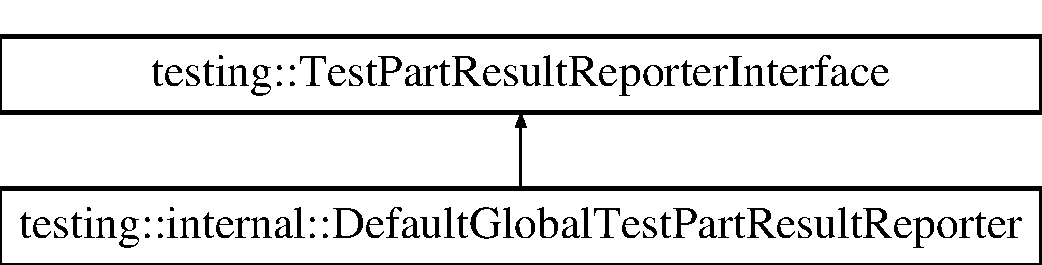
\includegraphics[height=2.000000cm]{classtesting_1_1internal_1_1_default_global_test_part_result_reporter}
\end{center}
\end{figure}
\subsection*{Public Member Functions}
\begin{DoxyCompactItemize}
\item 
\mbox{\Hypertarget{classtesting_1_1internal_1_1_default_global_test_part_result_reporter_a3900ea7f34b34afd48c7d1d0312a1488}\label{classtesting_1_1internal_1_1_default_global_test_part_result_reporter_a3900ea7f34b34afd48c7d1d0312a1488}} 
{\bfseries Default\+Global\+Test\+Part\+Result\+Reporter} (\mbox{\hyperlink{classtesting_1_1internal_1_1_unit_test_impl}{Unit\+Test\+Impl}} $\ast$unit\+\_\+test)
\item 
\mbox{\Hypertarget{classtesting_1_1internal_1_1_default_global_test_part_result_reporter_a6081576a23b964cfecab1e424d8044fc}\label{classtesting_1_1internal_1_1_default_global_test_part_result_reporter_a6081576a23b964cfecab1e424d8044fc}} 
virtual void {\bfseries Report\+Test\+Part\+Result} (const \mbox{\hyperlink{classtesting_1_1_test_part_result}{Test\+Part\+Result}} \&result)
\end{DoxyCompactItemize}


The documentation for this class was generated from the following files\+:\begin{DoxyCompactItemize}
\item 
/\+Users/fjp/git/bachelor/bachelor-\/master\+\_\+updated\+\_\+vfinal/googletest-\/1.\+8.\+0/googletest/src/gtest-\/internal-\/inl.\+h\item 
/\+Users/fjp/git/bachelor/bachelor-\/master\+\_\+updated\+\_\+vfinal/googletest-\/1.\+8.\+0/googletest/src/gtest.\+cc\end{DoxyCompactItemize}

\hypertarget{classtesting_1_1internal_1_1_default_per_thread_test_part_result_reporter}{}\section{testing\+:\+:internal\+:\+:Default\+Per\+Thread\+Test\+Part\+Result\+Reporter Class Reference}
\label{classtesting_1_1internal_1_1_default_per_thread_test_part_result_reporter}\index{testing\+::internal\+::\+Default\+Per\+Thread\+Test\+Part\+Result\+Reporter@{testing\+::internal\+::\+Default\+Per\+Thread\+Test\+Part\+Result\+Reporter}}
Inheritance diagram for testing\+:\+:internal\+:\+:Default\+Per\+Thread\+Test\+Part\+Result\+Reporter\+:\begin{figure}[H]
\begin{center}
\leavevmode
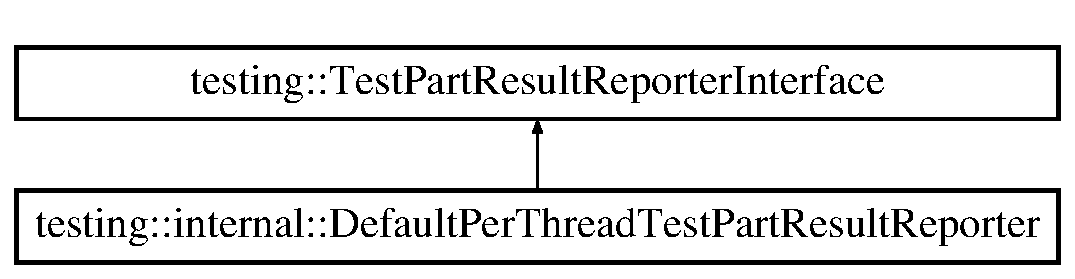
\includegraphics[height=2.000000cm]{classtesting_1_1internal_1_1_default_per_thread_test_part_result_reporter}
\end{center}
\end{figure}
\subsection*{Public Member Functions}
\begin{DoxyCompactItemize}
\item 
\mbox{\Hypertarget{classtesting_1_1internal_1_1_default_per_thread_test_part_result_reporter_a968a846e5a90d2ffea8b2ce2746099bd}\label{classtesting_1_1internal_1_1_default_per_thread_test_part_result_reporter_a968a846e5a90d2ffea8b2ce2746099bd}} 
{\bfseries Default\+Per\+Thread\+Test\+Part\+Result\+Reporter} (\mbox{\hyperlink{classtesting_1_1internal_1_1_unit_test_impl}{Unit\+Test\+Impl}} $\ast$unit\+\_\+test)
\item 
\mbox{\Hypertarget{classtesting_1_1internal_1_1_default_per_thread_test_part_result_reporter_ac6dc08eadc4e5a2a64a91d0b6c6b3aad}\label{classtesting_1_1internal_1_1_default_per_thread_test_part_result_reporter_ac6dc08eadc4e5a2a64a91d0b6c6b3aad}} 
virtual void {\bfseries Report\+Test\+Part\+Result} (const \mbox{\hyperlink{classtesting_1_1_test_part_result}{Test\+Part\+Result}} \&result)
\end{DoxyCompactItemize}


The documentation for this class was generated from the following files\+:\begin{DoxyCompactItemize}
\item 
/\+Users/fjp/git/bachelor/bachelor-\/master\+\_\+updated\+\_\+vfinal/googletest-\/1.\+8.\+0/googletest/src/gtest-\/internal-\/inl.\+h\item 
/\+Users/fjp/git/bachelor/bachelor-\/master\+\_\+updated\+\_\+vfinal/googletest-\/1.\+8.\+0/googletest/src/gtest.\+cc\end{DoxyCompactItemize}

\hypertarget{classtesting_1_1internal_1_1_derived}{}\section{testing\+:\+:internal\+:\+:Derived Class Reference}
\label{classtesting_1_1internal_1_1_derived}\index{testing\+::internal\+::\+Derived@{testing\+::internal\+::\+Derived}}
Inheritance diagram for testing\+:\+:internal\+:\+:Derived\+:\begin{figure}[H]
\begin{center}
\leavevmode
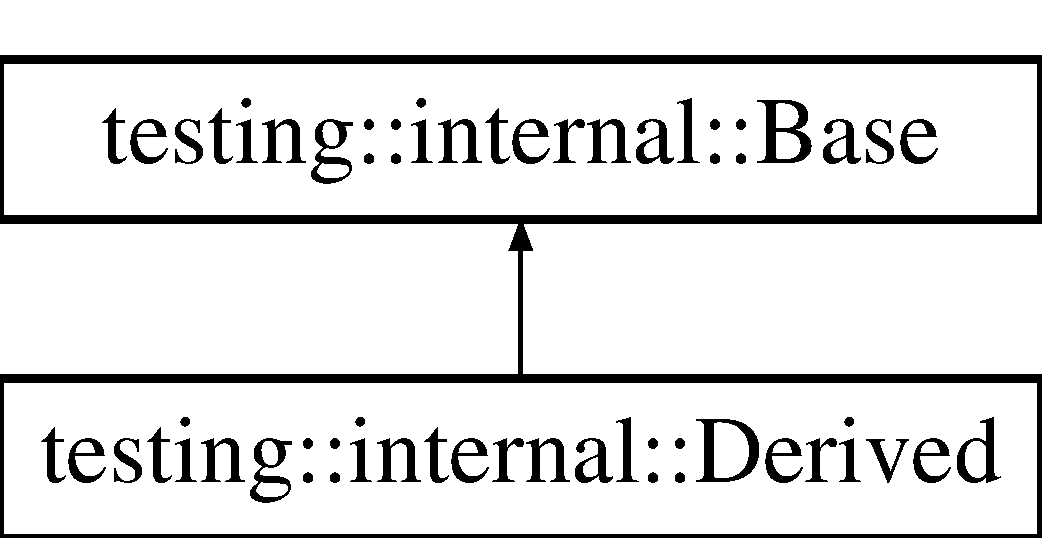
\includegraphics[height=2.000000cm]{classtesting_1_1internal_1_1_derived}
\end{center}
\end{figure}
\subsection*{Public Member Functions}
\begin{DoxyCompactItemize}
\item 
\mbox{\Hypertarget{classtesting_1_1internal_1_1_derived_a05a8e8354c7c09a9f3728a96c96f1edd}\label{classtesting_1_1internal_1_1_derived_a05a8e8354c7c09a9f3728a96c96f1edd}} 
{\bfseries Derived} (int n)
\end{DoxyCompactItemize}


The documentation for this class was generated from the following file\+:\begin{DoxyCompactItemize}
\item 
/\+Users/fjp/git/bachelor/bachelor-\/master\+\_\+updated\+\_\+vfinal/googletest-\/1.\+8.\+0/googletest/test/gtest-\/port\+\_\+test.\+cc\end{DoxyCompactItemize}

\hypertarget{class_disabled_test}{}\section{Disabled\+Test Class Reference}
\label{class_disabled_test}\index{Disabled\+Test@{Disabled\+Test}}
Inheritance diagram for Disabled\+Test\+:\begin{figure}[H]
\begin{center}
\leavevmode
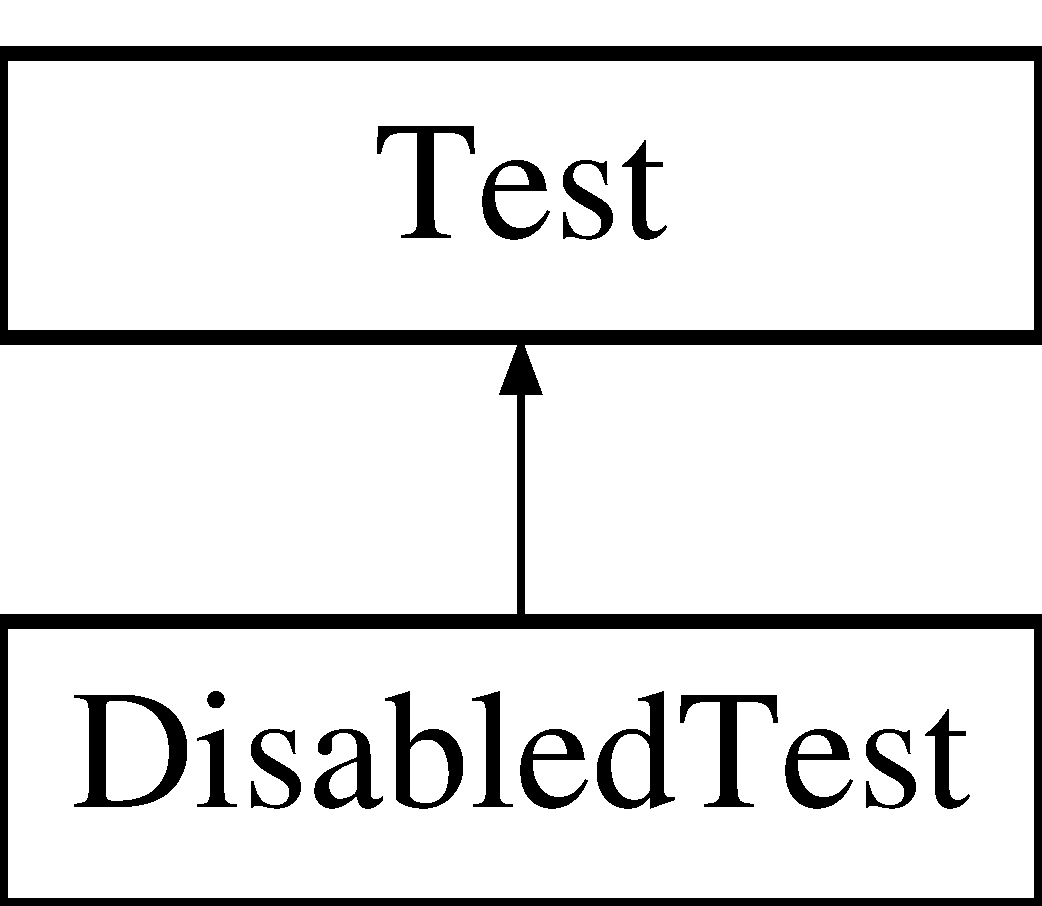
\includegraphics[height=2.000000cm]{class_disabled_test}
\end{center}
\end{figure}


The documentation for this class was generated from the following file\+:\begin{DoxyCompactItemize}
\item 
/\+Users/fjp/git/bachelor/bachelor-\/master\+\_\+updated\+\_\+vfinal/googletest-\/1.\+8.\+0/googletest/test/gtest\+\_\+xml\+\_\+output\+\_\+unittest\+\_\+.\+cc\end{DoxyCompactItemize}

\hypertarget{classpump_1_1_else_node}{}\section{pump.\+Else\+Node Class Reference}
\label{classpump_1_1_else_node}\index{pump.\+Else\+Node@{pump.\+Else\+Node}}
\subsection*{Public Member Functions}
\begin{DoxyCompactItemize}
\item 
\mbox{\Hypertarget{classpump_1_1_else_node_a7489ff8c6c7ddfe6bd6593b8ecccd819}\label{classpump_1_1_else_node_a7489ff8c6c7ddfe6bd6593b8ecccd819}} 
def {\bfseries \+\_\+\+\_\+init\+\_\+\+\_\+} (self, else\+\_\+branch=None)
\end{DoxyCompactItemize}
\subsection*{Public Attributes}
\begin{DoxyCompactItemize}
\item 
\mbox{\Hypertarget{classpump_1_1_else_node_ac838a0fe9f5d713c7f56939eed5e128d}\label{classpump_1_1_else_node_ac838a0fe9f5d713c7f56939eed5e128d}} 
{\bfseries else\+\_\+branch}
\end{DoxyCompactItemize}


The documentation for this class was generated from the following file\+:\begin{DoxyCompactItemize}
\item 
/\+Users/fjp/git/bachelor/bachelor-\/master\+\_\+updated\+\_\+vfinal/googletest-\/1.\+8.\+0/googletest/scripts/pump.\+py\end{DoxyCompactItemize}

\hypertarget{classtesting_1_1_empty_test_event_listener}{}\section{testing\+:\+:Empty\+Test\+Event\+Listener Class Reference}
\label{classtesting_1_1_empty_test_event_listener}\index{testing\+::\+Empty\+Test\+Event\+Listener@{testing\+::\+Empty\+Test\+Event\+Listener}}
Inheritance diagram for testing\+:\+:Empty\+Test\+Event\+Listener\+:\begin{figure}[H]
\begin{center}
\leavevmode
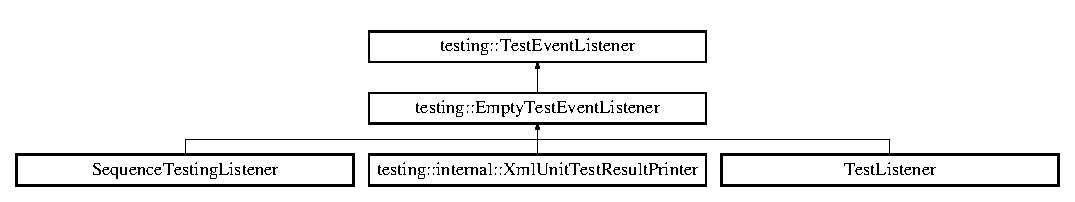
\includegraphics[height=2.267207cm]{classtesting_1_1_empty_test_event_listener}
\end{center}
\end{figure}
\subsection*{Public Member Functions}
\begin{DoxyCompactItemize}
\item 
\mbox{\Hypertarget{classtesting_1_1_empty_test_event_listener_aa3847c8a3c22d8d69a6006dfdd6589fc}\label{classtesting_1_1_empty_test_event_listener_aa3847c8a3c22d8d69a6006dfdd6589fc}} 
virtual void {\bfseries On\+Test\+Program\+Start} (const \mbox{\hyperlink{classtesting_1_1_unit_test}{Unit\+Test}} \&)
\item 
\mbox{\Hypertarget{classtesting_1_1_empty_test_event_listener_a836f05829855dc60d13ba99ad712c0dd}\label{classtesting_1_1_empty_test_event_listener_a836f05829855dc60d13ba99ad712c0dd}} 
virtual void {\bfseries On\+Test\+Iteration\+Start} (const \mbox{\hyperlink{classtesting_1_1_unit_test}{Unit\+Test}} \&, int)
\item 
\mbox{\Hypertarget{classtesting_1_1_empty_test_event_listener_a156d1965248fbdced6aabacadfa2d63f}\label{classtesting_1_1_empty_test_event_listener_a156d1965248fbdced6aabacadfa2d63f}} 
virtual void {\bfseries On\+Environments\+Set\+Up\+Start} (const \mbox{\hyperlink{classtesting_1_1_unit_test}{Unit\+Test}} \&)
\item 
\mbox{\Hypertarget{classtesting_1_1_empty_test_event_listener_abc481c6648d15d4242245195a06f5aa0}\label{classtesting_1_1_empty_test_event_listener_abc481c6648d15d4242245195a06f5aa0}} 
virtual void {\bfseries On\+Environments\+Set\+Up\+End} (const \mbox{\hyperlink{classtesting_1_1_unit_test}{Unit\+Test}} \&)
\item 
\mbox{\Hypertarget{classtesting_1_1_empty_test_event_listener_ae4707ed9cc7ace5241bc8ccc4051209b}\label{classtesting_1_1_empty_test_event_listener_ae4707ed9cc7ace5241bc8ccc4051209b}} 
virtual void {\bfseries On\+Test\+Case\+Start} (const \mbox{\hyperlink{classtesting_1_1_test_case}{Test\+Case}} \&)
\item 
\mbox{\Hypertarget{classtesting_1_1_empty_test_event_listener_a84fa74cc9ba742f9f847ea405ca84e5e}\label{classtesting_1_1_empty_test_event_listener_a84fa74cc9ba742f9f847ea405ca84e5e}} 
virtual void {\bfseries On\+Test\+Start} (const \mbox{\hyperlink{classtesting_1_1_test_info}{Test\+Info}} \&)
\item 
\mbox{\Hypertarget{classtesting_1_1_empty_test_event_listener_a59e7f7d9f2e2d089a6e8c1e2577f4718}\label{classtesting_1_1_empty_test_event_listener_a59e7f7d9f2e2d089a6e8c1e2577f4718}} 
virtual void {\bfseries On\+Test\+Part\+Result} (const \mbox{\hyperlink{classtesting_1_1_test_part_result}{Test\+Part\+Result}} \&)
\item 
\mbox{\Hypertarget{classtesting_1_1_empty_test_event_listener_afd58d21005f0d0d0399fb114627545d3}\label{classtesting_1_1_empty_test_event_listener_afd58d21005f0d0d0399fb114627545d3}} 
virtual void {\bfseries On\+Test\+End} (const \mbox{\hyperlink{classtesting_1_1_test_info}{Test\+Info}} \&)
\item 
\mbox{\Hypertarget{classtesting_1_1_empty_test_event_listener_a6bec703158283104c4298f7d8a528515}\label{classtesting_1_1_empty_test_event_listener_a6bec703158283104c4298f7d8a528515}} 
virtual void {\bfseries On\+Test\+Case\+End} (const \mbox{\hyperlink{classtesting_1_1_test_case}{Test\+Case}} \&)
\item 
\mbox{\Hypertarget{classtesting_1_1_empty_test_event_listener_a00fa1a4ea5831e20746188414268e7c6}\label{classtesting_1_1_empty_test_event_listener_a00fa1a4ea5831e20746188414268e7c6}} 
virtual void {\bfseries On\+Environments\+Tear\+Down\+Start} (const \mbox{\hyperlink{classtesting_1_1_unit_test}{Unit\+Test}} \&)
\item 
\mbox{\Hypertarget{classtesting_1_1_empty_test_event_listener_aea64c83c415b33a4c0b0239bafd1438d}\label{classtesting_1_1_empty_test_event_listener_aea64c83c415b33a4c0b0239bafd1438d}} 
virtual void {\bfseries On\+Environments\+Tear\+Down\+End} (const \mbox{\hyperlink{classtesting_1_1_unit_test}{Unit\+Test}} \&)
\item 
\mbox{\Hypertarget{classtesting_1_1_empty_test_event_listener_a2253e5a18b3cf7bccd349567a252209d}\label{classtesting_1_1_empty_test_event_listener_a2253e5a18b3cf7bccd349567a252209d}} 
virtual void {\bfseries On\+Test\+Iteration\+End} (const \mbox{\hyperlink{classtesting_1_1_unit_test}{Unit\+Test}} \&, int)
\item 
\mbox{\Hypertarget{classtesting_1_1_empty_test_event_listener_a0abcc02bd2331a2e29ad6f4d9daf2a32}\label{classtesting_1_1_empty_test_event_listener_a0abcc02bd2331a2e29ad6f4d9daf2a32}} 
virtual void {\bfseries On\+Test\+Program\+End} (const \mbox{\hyperlink{classtesting_1_1_unit_test}{Unit\+Test}} \&)
\end{DoxyCompactItemize}


The documentation for this class was generated from the following file\+:\begin{DoxyCompactItemize}
\item 
/\+Users/fjp/git/bachelor/bachelor-\/master\+\_\+updated\+\_\+vfinal/googletest-\/1.\+8.\+0/googletest/include/gtest/gtest.\+h\end{DoxyCompactItemize}

\hypertarget{structtesting_1_1internal_1_1_enable_if}{}\section{testing\+:\+:internal\+:\+:Enable\+If$<$ bool $>$ Struct Template Reference}
\label{structtesting_1_1internal_1_1_enable_if}\index{testing\+::internal\+::\+Enable\+If$<$ bool $>$@{testing\+::internal\+::\+Enable\+If$<$ bool $>$}}


The documentation for this struct was generated from the following file\+:\begin{DoxyCompactItemize}
\item 
/\+Users/fjp/git/bachelor/bachelor-\/master\+\_\+updated\+\_\+vfinal/googletest-\/1.\+8.\+0/googletest/include/gtest/internal/gtest-\/internal.\+h\end{DoxyCompactItemize}

\hypertarget{structtesting_1_1internal_1_1_enable_if_3_01true_01_4}{}\section{testing\+:\+:internal\+:\+:Enable\+If$<$ true $>$ Struct Template Reference}
\label{structtesting_1_1internal_1_1_enable_if_3_01true_01_4}\index{testing\+::internal\+::\+Enable\+If$<$ true $>$@{testing\+::internal\+::\+Enable\+If$<$ true $>$}}
\subsection*{Public Types}
\begin{DoxyCompactItemize}
\item 
\mbox{\Hypertarget{structtesting_1_1internal_1_1_enable_if_3_01true_01_4_a9398d803f1fdd99ff41823746f6299ff}\label{structtesting_1_1internal_1_1_enable_if_3_01true_01_4_a9398d803f1fdd99ff41823746f6299ff}} 
typedef void {\bfseries type}
\end{DoxyCompactItemize}


The documentation for this struct was generated from the following file\+:\begin{DoxyCompactItemize}
\item 
/\+Users/fjp/git/bachelor/bachelor-\/master\+\_\+updated\+\_\+vfinal/googletest-\/1.\+8.\+0/googletest/include/gtest/internal/gtest-\/internal.\+h\end{DoxyCompactItemize}

\hypertarget{classpump_1_1_env}{}\section{pump.\+Env Class Reference}
\label{classpump_1_1_env}\index{pump.\+Env@{pump.\+Env}}
\subsection*{Public Member Functions}
\begin{DoxyCompactItemize}
\item 
\mbox{\Hypertarget{classpump_1_1_env_a803732618a49ab4a2edf098b78081611}\label{classpump_1_1_env_a803732618a49ab4a2edf098b78081611}} 
def {\bfseries \+\_\+\+\_\+init\+\_\+\+\_\+} (self)
\item 
\mbox{\Hypertarget{classpump_1_1_env_a4c1b156cfa4aec708746bbe07dae5f1a}\label{classpump_1_1_env_a4c1b156cfa4aec708746bbe07dae5f1a}} 
def {\bfseries Clone} (self)
\item 
\mbox{\Hypertarget{classpump_1_1_env_ae0abc25733c61a8cc010cc5d76dd0dd8}\label{classpump_1_1_env_ae0abc25733c61a8cc010cc5d76dd0dd8}} 
def {\bfseries Push\+Variable} (self, var, value)
\item 
\mbox{\Hypertarget{classpump_1_1_env_abf35f8b971acedb275bb92bb29fcd587}\label{classpump_1_1_env_abf35f8b971acedb275bb92bb29fcd587}} 
def {\bfseries Pop\+Variable} (self)
\item 
\mbox{\Hypertarget{classpump_1_1_env_a600c34cac1e4ba75406efeadb2d7dd95}\label{classpump_1_1_env_a600c34cac1e4ba75406efeadb2d7dd95}} 
def {\bfseries Push\+Range} (self, var, lower, upper)
\item 
\mbox{\Hypertarget{classpump_1_1_env_a45474355fc03b69e7449199cc8012ba9}\label{classpump_1_1_env_a45474355fc03b69e7449199cc8012ba9}} 
def {\bfseries Pop\+Range} (self)
\item 
\mbox{\Hypertarget{classpump_1_1_env_a43c3609179d5e458266731199e35313b}\label{classpump_1_1_env_a43c3609179d5e458266731199e35313b}} 
def {\bfseries Get\+Value} (self, identifier)
\item 
\mbox{\Hypertarget{classpump_1_1_env_a29fa1ceb1f7c22e8e982133f4808317f}\label{classpump_1_1_env_a29fa1ceb1f7c22e8e982133f4808317f}} 
def {\bfseries Eval\+Exp} (self, exp)
\item 
\mbox{\Hypertarget{classpump_1_1_env_a1df05a550bdcfe4bb8c5b1608484a6dc}\label{classpump_1_1_env_a1df05a550bdcfe4bb8c5b1608484a6dc}} 
def {\bfseries Get\+Range} (self, identifier)
\end{DoxyCompactItemize}
\subsection*{Public Attributes}
\begin{DoxyCompactItemize}
\item 
\mbox{\Hypertarget{classpump_1_1_env_aba6456f3d0d23ac92bc9508c1b966bcd}\label{classpump_1_1_env_aba6456f3d0d23ac92bc9508c1b966bcd}} 
{\bfseries variables}
\item 
\mbox{\Hypertarget{classpump_1_1_env_a8d5fec087c1a9108de9b105922b34309}\label{classpump_1_1_env_a8d5fec087c1a9108de9b105922b34309}} 
{\bfseries ranges}
\end{DoxyCompactItemize}


The documentation for this class was generated from the following file\+:\begin{DoxyCompactItemize}
\item 
/\+Users/fjp/git/bachelor/bachelor-\/master\+\_\+updated\+\_\+vfinal/googletest-\/1.\+8.\+0/googletest/scripts/pump.\+py\end{DoxyCompactItemize}

\hypertarget{classtesting_1_1_environment}{}\section{testing\+:\+:Environment Class Reference}
\label{classtesting_1_1_environment}\index{testing\+::\+Environment@{testing\+::\+Environment}}
Inheritance diagram for testing\+:\+:Environment\+:\begin{figure}[H]
\begin{center}
\leavevmode
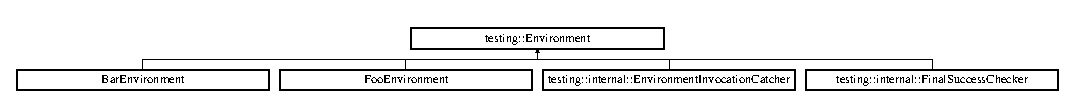
\includegraphics[height=0.989399cm]{classtesting_1_1_environment}
\end{center}
\end{figure}
\subsection*{Public Member Functions}
\begin{DoxyCompactItemize}
\item 
\mbox{\Hypertarget{classtesting_1_1_environment_a1bf8cafaa9d4eba9feb98655ee434eb3}\label{classtesting_1_1_environment_a1bf8cafaa9d4eba9feb98655ee434eb3}} 
virtual void {\bfseries Set\+Up} ()
\item 
\mbox{\Hypertarget{classtesting_1_1_environment_a039bdaa705c46b9b88234cf4d3bb6254}\label{classtesting_1_1_environment_a039bdaa705c46b9b88234cf4d3bb6254}} 
virtual void {\bfseries Tear\+Down} ()
\end{DoxyCompactItemize}


The documentation for this class was generated from the following file\+:\begin{DoxyCompactItemize}
\item 
/\+Users/fjp/git/bachelor/bachelor-\/master\+\_\+updated\+\_\+vfinal/googletest-\/1.\+8.\+0/googletest/include/gtest/gtest.\+h\end{DoxyCompactItemize}

\hypertarget{classtesting_1_1internal_1_1_environment_invocation_catcher}{}\section{testing\+:\+:internal\+:\+:Environment\+Invocation\+Catcher Class Reference}
\label{classtesting_1_1internal_1_1_environment_invocation_catcher}\index{testing\+::internal\+::\+Environment\+Invocation\+Catcher@{testing\+::internal\+::\+Environment\+Invocation\+Catcher}}
Inheritance diagram for testing\+:\+:internal\+:\+:Environment\+Invocation\+Catcher\+:\begin{figure}[H]
\begin{center}
\leavevmode
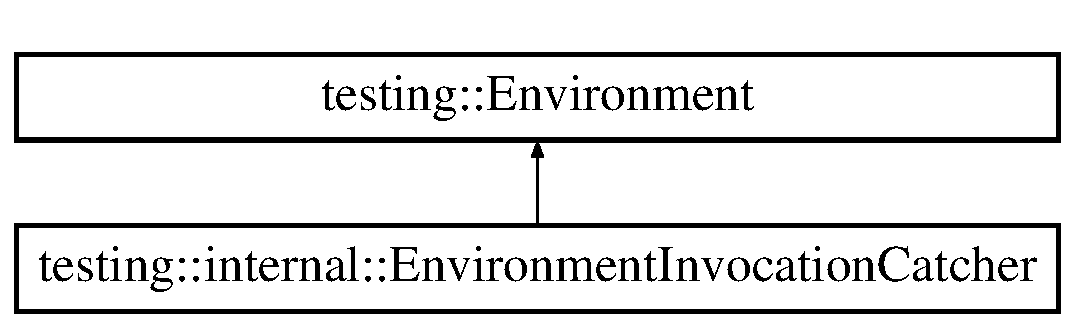
\includegraphics[height=2.000000cm]{classtesting_1_1internal_1_1_environment_invocation_catcher}
\end{center}
\end{figure}
\subsection*{Protected Member Functions}
\begin{DoxyCompactItemize}
\item 
\mbox{\Hypertarget{classtesting_1_1internal_1_1_environment_invocation_catcher_a325365b0ecfa71a4a767d7a1817c9663}\label{classtesting_1_1internal_1_1_environment_invocation_catcher_a325365b0ecfa71a4a767d7a1817c9663}} 
virtual void {\bfseries Set\+Up} ()
\item 
\mbox{\Hypertarget{classtesting_1_1internal_1_1_environment_invocation_catcher_afc89ee0a8e32e6746a89fcc1682f62e9}\label{classtesting_1_1internal_1_1_environment_invocation_catcher_afc89ee0a8e32e6746a89fcc1682f62e9}} 
virtual void {\bfseries Tear\+Down} ()
\end{DoxyCompactItemize}
\subsection*{Additional Inherited Members}


The documentation for this class was generated from the following file\+:\begin{DoxyCompactItemize}
\item 
/\+Users/fjp/git/bachelor/bachelor-\/master\+\_\+updated\+\_\+vfinal/googletest-\/1.\+8.\+0/googletest/test/gtest-\/listener\+\_\+test.\+cc\end{DoxyCompactItemize}

\hypertarget{classtesting_1_1internal_1_1_eq_helper}{}\section{testing\+:\+:internal\+:\+:Eq\+Helper$<$ lhs\+\_\+is\+\_\+null\+\_\+literal $>$ Class Template Reference}
\label{classtesting_1_1internal_1_1_eq_helper}\index{testing\+::internal\+::\+Eq\+Helper$<$ lhs\+\_\+is\+\_\+null\+\_\+literal $>$@{testing\+::internal\+::\+Eq\+Helper$<$ lhs\+\_\+is\+\_\+null\+\_\+literal $>$}}
\subsection*{Static Public Member Functions}
\begin{DoxyCompactItemize}
\item 
\mbox{\Hypertarget{classtesting_1_1internal_1_1_eq_helper_ae3572c7374534a916b9117efaa89f33f}\label{classtesting_1_1internal_1_1_eq_helper_ae3572c7374534a916b9117efaa89f33f}} 
{\footnotesize template$<$typename T1 , typename T2 $>$ }\\static \mbox{\hyperlink{classtesting_1_1_assertion_result}{Assertion\+Result}} {\bfseries Compare} (const char $\ast$lhs\+\_\+expression, const char $\ast$rhs\+\_\+expression, const T1 \&lhs, const T2 \&rhs)
\item 
\mbox{\Hypertarget{classtesting_1_1internal_1_1_eq_helper_aaa42c0059bb3dcc43d556243febb5f1c}\label{classtesting_1_1internal_1_1_eq_helper_aaa42c0059bb3dcc43d556243febb5f1c}} 
static \mbox{\hyperlink{classtesting_1_1_assertion_result}{Assertion\+Result}} {\bfseries Compare} (const char $\ast$lhs\+\_\+expression, const char $\ast$rhs\+\_\+expression, Biggest\+Int lhs, Biggest\+Int rhs)
\end{DoxyCompactItemize}


The documentation for this class was generated from the following file\+:\begin{DoxyCompactItemize}
\item 
/\+Users/fjp/git/bachelor/bachelor-\/master\+\_\+updated\+\_\+vfinal/googletest-\/1.\+8.\+0/googletest/include/gtest/gtest.\+h\end{DoxyCompactItemize}

\hypertarget{classtesting_1_1internal_1_1_eq_helper_3_01true_01_4}{}\section{testing\+:\+:internal\+:\+:Eq\+Helper$<$ true $>$ Class Template Reference}
\label{classtesting_1_1internal_1_1_eq_helper_3_01true_01_4}\index{testing\+::internal\+::\+Eq\+Helper$<$ true $>$@{testing\+::internal\+::\+Eq\+Helper$<$ true $>$}}
\subsection*{Static Public Member Functions}
\begin{DoxyCompactItemize}
\item 
\mbox{\Hypertarget{classtesting_1_1internal_1_1_eq_helper_3_01true_01_4_a12c7194b2a210b61f06c912eef484ca6}\label{classtesting_1_1internal_1_1_eq_helper_3_01true_01_4_a12c7194b2a210b61f06c912eef484ca6}} 
{\footnotesize template$<$typename T1 , typename T2 $>$ }\\static \mbox{\hyperlink{classtesting_1_1_assertion_result}{Assertion\+Result}} {\bfseries Compare} (const char $\ast$lhs\+\_\+expression, const char $\ast$rhs\+\_\+expression, const T1 \&lhs, const T2 \&rhs, typename \mbox{\hyperlink{structtesting_1_1internal_1_1_enable_if}{Enable\+If}}$<$!\mbox{\hyperlink{structtesting_1_1internal_1_1is__pointer}{is\+\_\+pointer}}$<$ T2 $>$\+::value $>$\+::type $\ast$=0)
\item 
\mbox{\Hypertarget{classtesting_1_1internal_1_1_eq_helper_3_01true_01_4_a6f292601a68c8f0d49e6d48bd309b900}\label{classtesting_1_1internal_1_1_eq_helper_3_01true_01_4_a6f292601a68c8f0d49e6d48bd309b900}} 
{\footnotesize template$<$typename T $>$ }\\static \mbox{\hyperlink{classtesting_1_1_assertion_result}{Assertion\+Result}} {\bfseries Compare} (const char $\ast$lhs\+\_\+expression, const char $\ast$rhs\+\_\+expression, Secret $\ast$, T $\ast$rhs)
\end{DoxyCompactItemize}


The documentation for this class was generated from the following file\+:\begin{DoxyCompactItemize}
\item 
/\+Users/fjp/git/bachelor/bachelor-\/master\+\_\+updated\+\_\+vfinal/googletest-\/1.\+8.\+0/googletest/include/gtest/gtest.\+h\end{DoxyCompactItemize}

\hypertarget{classtesting_1_1internal_1_1_event_recording_listener}{}\section{testing\+:\+:internal\+:\+:Event\+Recording\+Listener Class Reference}
\label{classtesting_1_1internal_1_1_event_recording_listener}\index{testing\+::internal\+::\+Event\+Recording\+Listener@{testing\+::internal\+::\+Event\+Recording\+Listener}}
Inheritance diagram for testing\+:\+:internal\+:\+:Event\+Recording\+Listener\+:\begin{figure}[H]
\begin{center}
\leavevmode
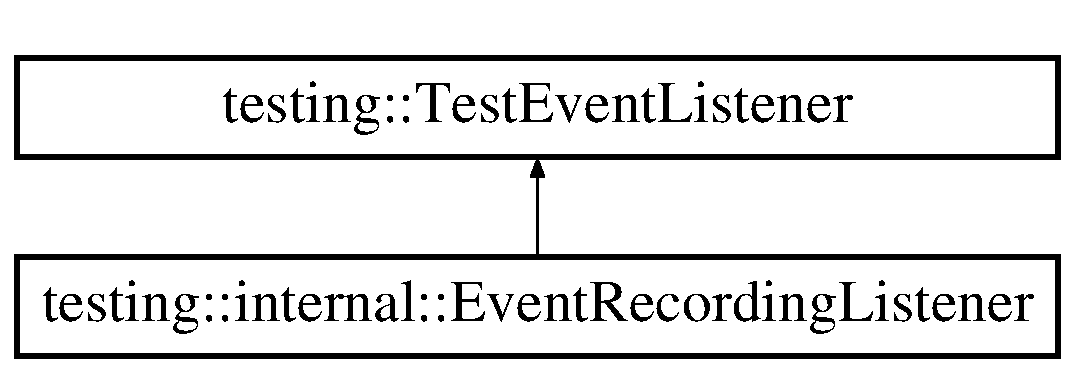
\includegraphics[height=2.000000cm]{classtesting_1_1internal_1_1_event_recording_listener}
\end{center}
\end{figure}
\subsection*{Public Member Functions}
\begin{DoxyCompactItemize}
\item 
\mbox{\Hypertarget{classtesting_1_1internal_1_1_event_recording_listener_a7b0254c15d6b8468e1441ee572fee707}\label{classtesting_1_1internal_1_1_event_recording_listener_a7b0254c15d6b8468e1441ee572fee707}} 
{\bfseries Event\+Recording\+Listener} (const char $\ast$name)
\end{DoxyCompactItemize}
\subsection*{Protected Member Functions}
\begin{DoxyCompactItemize}
\item 
\mbox{\Hypertarget{classtesting_1_1internal_1_1_event_recording_listener_aff89fdd3ae889a54a2ba2f3d4c98d3f6}\label{classtesting_1_1internal_1_1_event_recording_listener_aff89fdd3ae889a54a2ba2f3d4c98d3f6}} 
virtual void {\bfseries On\+Test\+Program\+Start} (const \mbox{\hyperlink{classtesting_1_1_unit_test}{Unit\+Test}} \&)
\item 
\mbox{\Hypertarget{classtesting_1_1internal_1_1_event_recording_listener_a0bfa276def9594b2a119c2c370f59281}\label{classtesting_1_1internal_1_1_event_recording_listener_a0bfa276def9594b2a119c2c370f59281}} 
virtual void {\bfseries On\+Test\+Iteration\+Start} (const \mbox{\hyperlink{classtesting_1_1_unit_test}{Unit\+Test}} \&, int iteration)
\item 
\mbox{\Hypertarget{classtesting_1_1internal_1_1_event_recording_listener_add61e6e7ebffb8afc90ccabcdc9f9982}\label{classtesting_1_1internal_1_1_event_recording_listener_add61e6e7ebffb8afc90ccabcdc9f9982}} 
virtual void {\bfseries On\+Environments\+Set\+Up\+Start} (const \mbox{\hyperlink{classtesting_1_1_unit_test}{Unit\+Test}} \&)
\item 
\mbox{\Hypertarget{classtesting_1_1internal_1_1_event_recording_listener_a40b4c5e05abd1aa11a030f999f6adb8f}\label{classtesting_1_1internal_1_1_event_recording_listener_a40b4c5e05abd1aa11a030f999f6adb8f}} 
virtual void {\bfseries On\+Environments\+Set\+Up\+End} (const \mbox{\hyperlink{classtesting_1_1_unit_test}{Unit\+Test}} \&)
\item 
\mbox{\Hypertarget{classtesting_1_1internal_1_1_event_recording_listener_a18c28e1d1c3a1e74e225966456786f8e}\label{classtesting_1_1internal_1_1_event_recording_listener_a18c28e1d1c3a1e74e225966456786f8e}} 
virtual void {\bfseries On\+Test\+Case\+Start} (const \mbox{\hyperlink{classtesting_1_1_test_case}{Test\+Case}} \&)
\item 
\mbox{\Hypertarget{classtesting_1_1internal_1_1_event_recording_listener_aebd488b780fc172d6058ca07ca8f7145}\label{classtesting_1_1internal_1_1_event_recording_listener_aebd488b780fc172d6058ca07ca8f7145}} 
virtual void {\bfseries On\+Test\+Start} (const \mbox{\hyperlink{classtesting_1_1_test_info}{Test\+Info}} \&)
\item 
\mbox{\Hypertarget{classtesting_1_1internal_1_1_event_recording_listener_a4a6685d894923f1691ad9c6a4311470e}\label{classtesting_1_1internal_1_1_event_recording_listener_a4a6685d894923f1691ad9c6a4311470e}} 
virtual void {\bfseries On\+Test\+Part\+Result} (const \mbox{\hyperlink{classtesting_1_1_test_part_result}{Test\+Part\+Result}} \&)
\item 
\mbox{\Hypertarget{classtesting_1_1internal_1_1_event_recording_listener_adb076f145cc20d9b27441b9c75da4b81}\label{classtesting_1_1internal_1_1_event_recording_listener_adb076f145cc20d9b27441b9c75da4b81}} 
virtual void {\bfseries On\+Test\+End} (const \mbox{\hyperlink{classtesting_1_1_test_info}{Test\+Info}} \&)
\item 
\mbox{\Hypertarget{classtesting_1_1internal_1_1_event_recording_listener_a4d0cb8a389c7339bce0aa6128291529f}\label{classtesting_1_1internal_1_1_event_recording_listener_a4d0cb8a389c7339bce0aa6128291529f}} 
virtual void {\bfseries On\+Test\+Case\+End} (const \mbox{\hyperlink{classtesting_1_1_test_case}{Test\+Case}} \&)
\item 
\mbox{\Hypertarget{classtesting_1_1internal_1_1_event_recording_listener_a17eebd7bb5cc6bab53b20794919ca5ae}\label{classtesting_1_1internal_1_1_event_recording_listener_a17eebd7bb5cc6bab53b20794919ca5ae}} 
virtual void {\bfseries On\+Environments\+Tear\+Down\+Start} (const \mbox{\hyperlink{classtesting_1_1_unit_test}{Unit\+Test}} \&)
\item 
\mbox{\Hypertarget{classtesting_1_1internal_1_1_event_recording_listener_acd5a3dc070265166a7da68222031fd61}\label{classtesting_1_1internal_1_1_event_recording_listener_acd5a3dc070265166a7da68222031fd61}} 
virtual void {\bfseries On\+Environments\+Tear\+Down\+End} (const \mbox{\hyperlink{classtesting_1_1_unit_test}{Unit\+Test}} \&)
\item 
\mbox{\Hypertarget{classtesting_1_1internal_1_1_event_recording_listener_ab0cc007bcfaf06cd383d574c88f62aea}\label{classtesting_1_1internal_1_1_event_recording_listener_ab0cc007bcfaf06cd383d574c88f62aea}} 
virtual void {\bfseries On\+Test\+Iteration\+End} (const \mbox{\hyperlink{classtesting_1_1_unit_test}{Unit\+Test}} \&, int iteration)
\item 
\mbox{\Hypertarget{classtesting_1_1internal_1_1_event_recording_listener_a21fe9c3c519c4599a48b16ddfb734aa3}\label{classtesting_1_1internal_1_1_event_recording_listener_a21fe9c3c519c4599a48b16ddfb734aa3}} 
virtual void {\bfseries On\+Test\+Program\+End} (const \mbox{\hyperlink{classtesting_1_1_unit_test}{Unit\+Test}} \&)
\end{DoxyCompactItemize}


The documentation for this class was generated from the following file\+:\begin{DoxyCompactItemize}
\item 
/\+Users/fjp/git/bachelor/bachelor-\/master\+\_\+updated\+\_\+vfinal/googletest-\/1.\+8.\+0/googletest/test/gtest-\/listener\+\_\+test.\+cc\end{DoxyCompactItemize}

\hypertarget{class_expect_failure_test}{}\section{Expect\+Failure\+Test Class Reference}
\label{class_expect_failure_test}\index{Expect\+Failure\+Test@{Expect\+Failure\+Test}}
Inheritance diagram for Expect\+Failure\+Test\+:\begin{figure}[H]
\begin{center}
\leavevmode
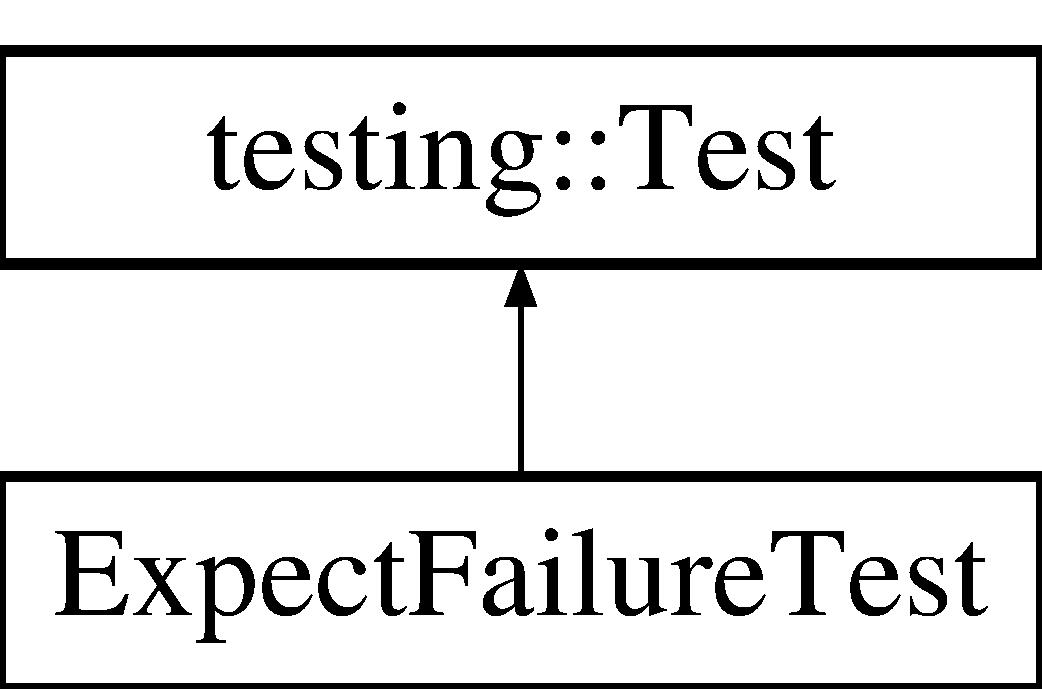
\includegraphics[height=2.000000cm]{class_expect_failure_test}
\end{center}
\end{figure}
\subsection*{Public Types}
\begin{DoxyCompactItemize}
\item 
\mbox{\Hypertarget{class_expect_failure_test_aad05da10bb15d21a434eba3b37011406}\label{class_expect_failure_test_aad05da10bb15d21a434eba3b37011406}} 
enum {\bfseries Failure\+Mode} \{ {\bfseries F\+A\+T\+A\+L\+\_\+\+F\+A\+I\+L\+U\+RE}, 
{\bfseries N\+O\+N\+F\+A\+T\+A\+L\+\_\+\+F\+A\+I\+L\+U\+RE}
 \}
\end{DoxyCompactItemize}
\subsection*{Static Public Member Functions}
\begin{DoxyCompactItemize}
\item 
\mbox{\Hypertarget{class_expect_failure_test_ab9aeb7820ff7953fc2975ecc5abd046b}\label{class_expect_failure_test_ab9aeb7820ff7953fc2975ecc5abd046b}} 
static void {\bfseries Add\+Failure} (Failure\+Mode failure)
\end{DoxyCompactItemize}
\subsection*{Additional Inherited Members}


The documentation for this class was generated from the following file\+:\begin{DoxyCompactItemize}
\item 
/\+Users/fjp/git/bachelor/bachelor-\/master\+\_\+updated\+\_\+vfinal/googletest-\/1.\+8.\+0/googletest/test/gtest\+\_\+output\+\_\+test\+\_\+.\+cc\end{DoxyCompactItemize}

\hypertarget{classpump_1_1_exp_node}{}\section{pump.\+Exp\+Node Class Reference}
\label{classpump_1_1_exp_node}\index{pump.\+Exp\+Node@{pump.\+Exp\+Node}}
\subsection*{Public Member Functions}
\begin{DoxyCompactItemize}
\item 
\mbox{\Hypertarget{classpump_1_1_exp_node_a0808c394c4d3c8ac875005caa1b3e1b3}\label{classpump_1_1_exp_node_a0808c394c4d3c8ac875005caa1b3e1b3}} 
def {\bfseries \+\_\+\+\_\+init\+\_\+\+\_\+} (self, token, python\+\_\+exp)
\end{DoxyCompactItemize}
\subsection*{Public Attributes}
\begin{DoxyCompactItemize}
\item 
\mbox{\Hypertarget{classpump_1_1_exp_node_ade05a5a32535d717dc5c194569aaf356}\label{classpump_1_1_exp_node_ade05a5a32535d717dc5c194569aaf356}} 
{\bfseries token}
\item 
\mbox{\Hypertarget{classpump_1_1_exp_node_adccfe4778c2e34f6b2c88118c0f1587f}\label{classpump_1_1_exp_node_adccfe4778c2e34f6b2c88118c0f1587f}} 
{\bfseries python\+\_\+exp}
\end{DoxyCompactItemize}


The documentation for this class was generated from the following file\+:\begin{DoxyCompactItemize}
\item 
/\+Users/fjp/git/bachelor/bachelor-\/master\+\_\+updated\+\_\+vfinal/googletest-\/1.\+8.\+0/googletest/scripts/pump.\+py\end{DoxyCompactItemize}

\hypertarget{class_failed_test}{}\section{Failed\+Test Class Reference}
\label{class_failed_test}\index{Failed\+Test@{Failed\+Test}}
Inheritance diagram for Failed\+Test\+:\begin{figure}[H]
\begin{center}
\leavevmode
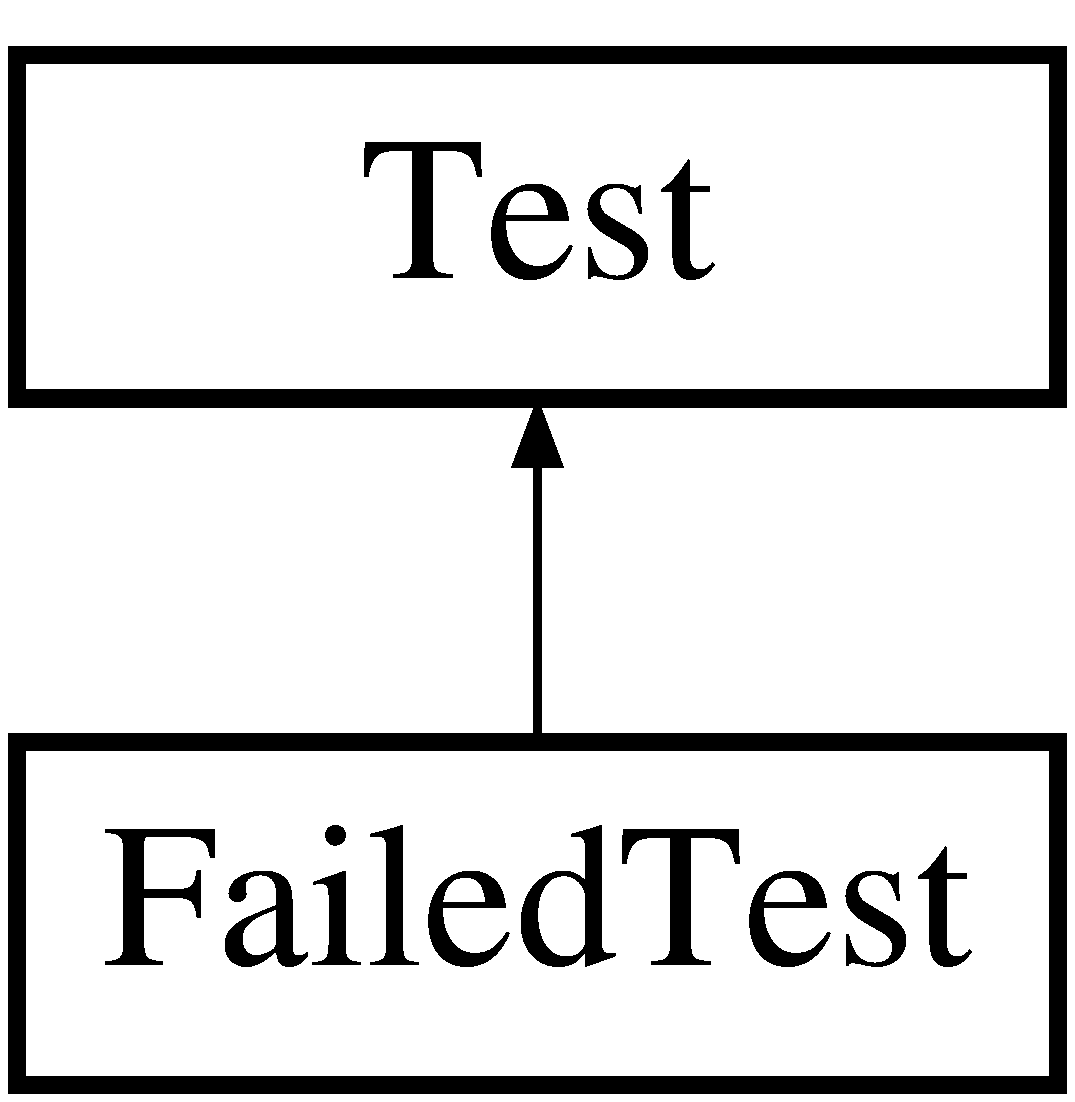
\includegraphics[height=2.000000cm]{class_failed_test}
\end{center}
\end{figure}


The documentation for this class was generated from the following file\+:\begin{DoxyCompactItemize}
\item 
/\+Users/fjp/git/bachelor/bachelor-\/master\+\_\+updated\+\_\+vfinal/googletest-\/1.\+8.\+0/googletest/test/gtest\+\_\+xml\+\_\+output\+\_\+unittest\+\_\+.\+cc\end{DoxyCompactItemize}

\hypertarget{class_failing_param_test}{}\section{Failing\+Param\+Test Class Reference}
\label{class_failing_param_test}\index{Failing\+Param\+Test@{Failing\+Param\+Test}}
Inheritance diagram for Failing\+Param\+Test\+:\begin{figure}[H]
\begin{center}
\leavevmode
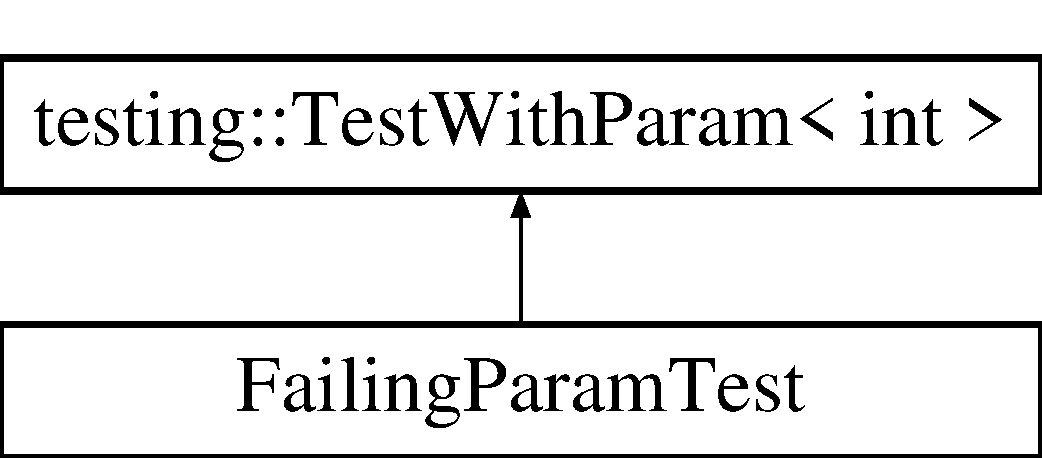
\includegraphics[height=2.000000cm]{class_failing_param_test}
\end{center}
\end{figure}


The documentation for this class was generated from the following file\+:\begin{DoxyCompactItemize}
\item 
/\+Users/fjp/git/bachelor/bachelor-\/master\+\_\+updated\+\_\+vfinal/googletest-\/1.\+8.\+0/googletest/test/gtest\+\_\+output\+\_\+test\+\_\+.\+cc\end{DoxyCompactItemize}

\hypertarget{class_fatal_failure_in_fixture_constructor_test}{}\section{Fatal\+Failure\+In\+Fixture\+Constructor\+Test Class Reference}
\label{class_fatal_failure_in_fixture_constructor_test}\index{Fatal\+Failure\+In\+Fixture\+Constructor\+Test@{Fatal\+Failure\+In\+Fixture\+Constructor\+Test}}
Inheritance diagram for Fatal\+Failure\+In\+Fixture\+Constructor\+Test\+:\begin{figure}[H]
\begin{center}
\leavevmode
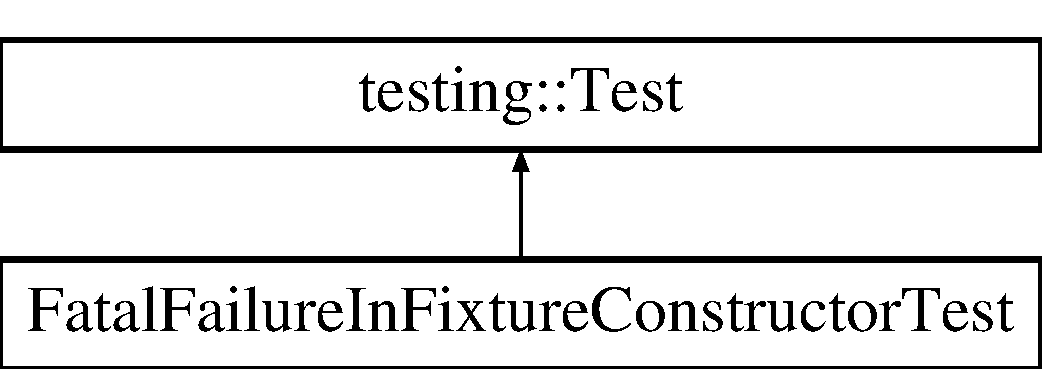
\includegraphics[height=2.000000cm]{class_fatal_failure_in_fixture_constructor_test}
\end{center}
\end{figure}
\subsection*{Protected Member Functions}
\begin{DoxyCompactItemize}
\item 
\mbox{\Hypertarget{class_fatal_failure_in_fixture_constructor_test_a006d3ac0e7a4ad3c469c3b41dc7c42c3}\label{class_fatal_failure_in_fixture_constructor_test_a006d3ac0e7a4ad3c469c3b41dc7c42c3}} 
virtual void {\bfseries Set\+Up} ()
\item 
\mbox{\Hypertarget{class_fatal_failure_in_fixture_constructor_test_a2763026a557e1fce4e59bd16c4eced57}\label{class_fatal_failure_in_fixture_constructor_test_a2763026a557e1fce4e59bd16c4eced57}} 
virtual void {\bfseries Tear\+Down} ()
\end{DoxyCompactItemize}
\subsection*{Additional Inherited Members}


The documentation for this class was generated from the following file\+:\begin{DoxyCompactItemize}
\item 
/\+Users/fjp/git/bachelor/bachelor-\/master\+\_\+updated\+\_\+vfinal/googletest-\/1.\+8.\+0/googletest/test/gtest\+\_\+output\+\_\+test\+\_\+.\+cc\end{DoxyCompactItemize}

\hypertarget{class_fatal_failure_in_set_up_test}{}\section{Fatal\+Failure\+In\+Set\+Up\+Test Class Reference}
\label{class_fatal_failure_in_set_up_test}\index{Fatal\+Failure\+In\+Set\+Up\+Test@{Fatal\+Failure\+In\+Set\+Up\+Test}}
Inheritance diagram for Fatal\+Failure\+In\+Set\+Up\+Test\+:\begin{figure}[H]
\begin{center}
\leavevmode
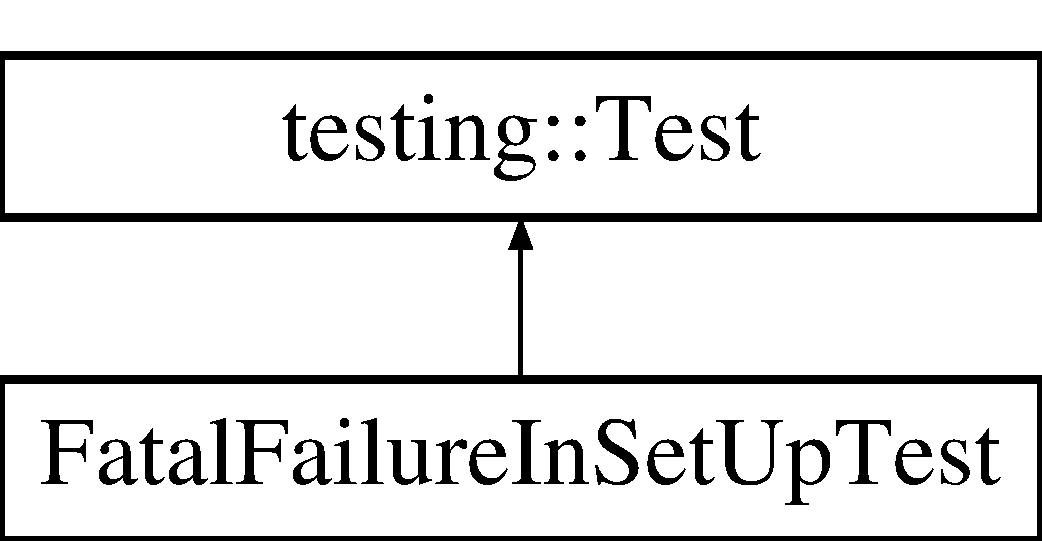
\includegraphics[height=2.000000cm]{class_fatal_failure_in_set_up_test}
\end{center}
\end{figure}
\subsection*{Protected Member Functions}
\begin{DoxyCompactItemize}
\item 
\mbox{\Hypertarget{class_fatal_failure_in_set_up_test_a455696f86fb5f5393624221ccb79b373}\label{class_fatal_failure_in_set_up_test_a455696f86fb5f5393624221ccb79b373}} 
virtual void {\bfseries Set\+Up} ()
\item 
\mbox{\Hypertarget{class_fatal_failure_in_set_up_test_a457707161063e08f7b6600ec5db449e4}\label{class_fatal_failure_in_set_up_test_a457707161063e08f7b6600ec5db449e4}} 
virtual void {\bfseries Tear\+Down} ()
\end{DoxyCompactItemize}
\subsection*{Additional Inherited Members}


The documentation for this class was generated from the following file\+:\begin{DoxyCompactItemize}
\item 
/\+Users/fjp/git/bachelor/bachelor-\/master\+\_\+updated\+\_\+vfinal/googletest-\/1.\+8.\+0/googletest/test/gtest\+\_\+output\+\_\+test\+\_\+.\+cc\end{DoxyCompactItemize}

\hypertarget{structvisualizer_1_1_file_header}{}\section{visualizer\+:\+:File\+Header Struct Reference}
\label{structvisualizer_1_1_file_header}\index{visualizer\+::\+File\+Header@{visualizer\+::\+File\+Header}}
\subsection*{Public Attributes}
\begin{DoxyCompactItemize}
\item 
\mbox{\Hypertarget{structvisualizer_1_1_file_header_a0a34468b872f064c94cefc09f2945c6e}\label{structvisualizer_1_1_file_header_a0a34468b872f064c94cefc09f2945c6e}} 
uint8\+\_\+t {\bfseries signature} \mbox{[}2\mbox{]}
\item 
\mbox{\Hypertarget{structvisualizer_1_1_file_header_ad79e04a6e593e9448a151049ef8290ab}\label{structvisualizer_1_1_file_header_ad79e04a6e593e9448a151049ef8290ab}} 
uint32\+\_\+t {\bfseries filesize}
\item 
\mbox{\Hypertarget{structvisualizer_1_1_file_header_abe8a37ffc28ff244e92680e8563537c5}\label{structvisualizer_1_1_file_header_abe8a37ffc28ff244e92680e8563537c5}} 
uint32\+\_\+t {\bfseries reserved}
\item 
\mbox{\Hypertarget{structvisualizer_1_1_file_header_ab24f1ce618c07cdfd8afc2b3d4455d3b}\label{structvisualizer_1_1_file_header_ab24f1ce618c07cdfd8afc2b3d4455d3b}} 
uint32\+\_\+t {\bfseries fileoffset\+\_\+to\+\_\+pixelarray}
\end{DoxyCompactItemize}


The documentation for this struct was generated from the following file\+:\begin{DoxyCompactItemize}
\item 
/\+Users/fjp/git/bachelor/bachelor-\/master\+\_\+updated\+\_\+vfinal/visualizer/visualizer.\+cpp\end{DoxyCompactItemize}

\hypertarget{classtesting_1_1internal_1_1_file_path}{}\section{testing\+:\+:internal\+:\+:File\+Path Class Reference}
\label{classtesting_1_1internal_1_1_file_path}\index{testing\+::internal\+::\+File\+Path@{testing\+::internal\+::\+File\+Path}}
\subsection*{Public Member Functions}
\begin{DoxyCompactItemize}
\item 
\mbox{\Hypertarget{classtesting_1_1internal_1_1_file_path_ae9efd0fee56c6e3e2d659b464250b112}\label{classtesting_1_1internal_1_1_file_path_ae9efd0fee56c6e3e2d659b464250b112}} 
{\bfseries File\+Path} (const \mbox{\hyperlink{classtesting_1_1internal_1_1_file_path}{File\+Path}} \&rhs)
\item 
\mbox{\Hypertarget{classtesting_1_1internal_1_1_file_path_a9fc072b140aa0652a7022fb809fe3abe}\label{classtesting_1_1internal_1_1_file_path_a9fc072b140aa0652a7022fb809fe3abe}} 
{\bfseries File\+Path} (const std\+::string \&pathname)
\item 
\mbox{\Hypertarget{classtesting_1_1internal_1_1_file_path_a8d9c1bafb90f10bcd5611a54d8f326ef}\label{classtesting_1_1internal_1_1_file_path_a8d9c1bafb90f10bcd5611a54d8f326ef}} 
\mbox{\hyperlink{classtesting_1_1internal_1_1_file_path}{File\+Path}} \& {\bfseries operator=} (const \mbox{\hyperlink{classtesting_1_1internal_1_1_file_path}{File\+Path}} \&rhs)
\item 
\mbox{\Hypertarget{classtesting_1_1internal_1_1_file_path_a15a42de7518e89254e0640dd9317d5f7}\label{classtesting_1_1internal_1_1_file_path_a15a42de7518e89254e0640dd9317d5f7}} 
void {\bfseries Set} (const \mbox{\hyperlink{classtesting_1_1internal_1_1_file_path}{File\+Path}} \&rhs)
\item 
\mbox{\Hypertarget{classtesting_1_1internal_1_1_file_path_ab1d58734f2e179264eb6353fea57361d}\label{classtesting_1_1internal_1_1_file_path_ab1d58734f2e179264eb6353fea57361d}} 
const std\+::string \& {\bfseries string} () const
\item 
\mbox{\Hypertarget{classtesting_1_1internal_1_1_file_path_a43e9ff978b0d7c43c401d976d4621aa3}\label{classtesting_1_1internal_1_1_file_path_a43e9ff978b0d7c43c401d976d4621aa3}} 
const char $\ast$ {\bfseries c\+\_\+str} () const
\item 
\mbox{\Hypertarget{classtesting_1_1internal_1_1_file_path_a2c165c5510e8705ade547849a9234a6e}\label{classtesting_1_1internal_1_1_file_path_a2c165c5510e8705ade547849a9234a6e}} 
bool {\bfseries Is\+Empty} () const
\item 
\mbox{\Hypertarget{classtesting_1_1internal_1_1_file_path_ab47ada111cc940cf2359f6533bada6ca}\label{classtesting_1_1internal_1_1_file_path_ab47ada111cc940cf2359f6533bada6ca}} 
\mbox{\hyperlink{classtesting_1_1internal_1_1_file_path}{File\+Path}} {\bfseries Remove\+Trailing\+Path\+Separator} () const
\item 
\mbox{\Hypertarget{classtesting_1_1internal_1_1_file_path_a6b61ede2c81ecd870b8220c04aec3060}\label{classtesting_1_1internal_1_1_file_path_a6b61ede2c81ecd870b8220c04aec3060}} 
\mbox{\hyperlink{classtesting_1_1internal_1_1_file_path}{File\+Path}} {\bfseries Remove\+Directory\+Name} () const
\item 
\mbox{\Hypertarget{classtesting_1_1internal_1_1_file_path_a49e030b5a62ca7dcc7f920a63a96fa55}\label{classtesting_1_1internal_1_1_file_path_a49e030b5a62ca7dcc7f920a63a96fa55}} 
\mbox{\hyperlink{classtesting_1_1internal_1_1_file_path}{File\+Path}} {\bfseries Remove\+File\+Name} () const
\item 
\mbox{\Hypertarget{classtesting_1_1internal_1_1_file_path_aab20b631705b90044d04c67205f2256f}\label{classtesting_1_1internal_1_1_file_path_aab20b631705b90044d04c67205f2256f}} 
\mbox{\hyperlink{classtesting_1_1internal_1_1_file_path}{File\+Path}} {\bfseries Remove\+Extension} (const char $\ast$extension) const
\item 
\mbox{\Hypertarget{classtesting_1_1internal_1_1_file_path_a26790e530dd738f7fc8202c1ce718406}\label{classtesting_1_1internal_1_1_file_path_a26790e530dd738f7fc8202c1ce718406}} 
bool {\bfseries Create\+Directories\+Recursively} () const
\item 
\mbox{\Hypertarget{classtesting_1_1internal_1_1_file_path_ae3a455e7c9fc967c2443b703e958f8bd}\label{classtesting_1_1internal_1_1_file_path_ae3a455e7c9fc967c2443b703e958f8bd}} 
bool {\bfseries Create\+Folder} () const
\item 
\mbox{\Hypertarget{classtesting_1_1internal_1_1_file_path_a105bd8fc3adff8fcb4a593532842fb68}\label{classtesting_1_1internal_1_1_file_path_a105bd8fc3adff8fcb4a593532842fb68}} 
bool {\bfseries File\+Or\+Directory\+Exists} () const
\item 
\mbox{\Hypertarget{classtesting_1_1internal_1_1_file_path_a74ba8435e822d77f79f137c38de9bfeb}\label{classtesting_1_1internal_1_1_file_path_a74ba8435e822d77f79f137c38de9bfeb}} 
bool {\bfseries Directory\+Exists} () const
\item 
\mbox{\Hypertarget{classtesting_1_1internal_1_1_file_path_a73fc042ad65e85bbecb956eb4603a6f2}\label{classtesting_1_1internal_1_1_file_path_a73fc042ad65e85bbecb956eb4603a6f2}} 
bool {\bfseries Is\+Directory} () const
\item 
\mbox{\Hypertarget{classtesting_1_1internal_1_1_file_path_a0661adf59aec40c40c8e39b888d68142}\label{classtesting_1_1internal_1_1_file_path_a0661adf59aec40c40c8e39b888d68142}} 
bool {\bfseries Is\+Root\+Directory} () const
\item 
\mbox{\Hypertarget{classtesting_1_1internal_1_1_file_path_ae17e5581e7996021e598851fe947df9c}\label{classtesting_1_1internal_1_1_file_path_ae17e5581e7996021e598851fe947df9c}} 
bool {\bfseries Is\+Absolute\+Path} () const
\end{DoxyCompactItemize}
\subsection*{Static Public Member Functions}
\begin{DoxyCompactItemize}
\item 
\mbox{\Hypertarget{classtesting_1_1internal_1_1_file_path_aaff39ccd7bfb7a1c09c0220a64326387}\label{classtesting_1_1internal_1_1_file_path_aaff39ccd7bfb7a1c09c0220a64326387}} 
static \mbox{\hyperlink{classtesting_1_1internal_1_1_file_path}{File\+Path}} {\bfseries Get\+Current\+Dir} ()
\item 
\mbox{\Hypertarget{classtesting_1_1internal_1_1_file_path_aa8c102da670261eb4fa8e2f2481df139}\label{classtesting_1_1internal_1_1_file_path_aa8c102da670261eb4fa8e2f2481df139}} 
static \mbox{\hyperlink{classtesting_1_1internal_1_1_file_path}{File\+Path}} {\bfseries Make\+File\+Name} (const \mbox{\hyperlink{classtesting_1_1internal_1_1_file_path}{File\+Path}} \&directory, const \mbox{\hyperlink{classtesting_1_1internal_1_1_file_path}{File\+Path}} \&base\+\_\+name, int number, const char $\ast$extension)
\item 
\mbox{\Hypertarget{classtesting_1_1internal_1_1_file_path_ac9d57987f60ac43f0c57b89e333e531e}\label{classtesting_1_1internal_1_1_file_path_ac9d57987f60ac43f0c57b89e333e531e}} 
static \mbox{\hyperlink{classtesting_1_1internal_1_1_file_path}{File\+Path}} {\bfseries Concat\+Paths} (const \mbox{\hyperlink{classtesting_1_1internal_1_1_file_path}{File\+Path}} \&directory, const \mbox{\hyperlink{classtesting_1_1internal_1_1_file_path}{File\+Path}} \&relative\+\_\+path)
\item 
\mbox{\Hypertarget{classtesting_1_1internal_1_1_file_path_a2280a77adb394cf80bb5f73fc292e8c8}\label{classtesting_1_1internal_1_1_file_path_a2280a77adb394cf80bb5f73fc292e8c8}} 
static \mbox{\hyperlink{classtesting_1_1internal_1_1_file_path}{File\+Path}} {\bfseries Generate\+Unique\+File\+Name} (const \mbox{\hyperlink{classtesting_1_1internal_1_1_file_path}{File\+Path}} \&directory, const \mbox{\hyperlink{classtesting_1_1internal_1_1_file_path}{File\+Path}} \&base\+\_\+name, const char $\ast$extension)
\end{DoxyCompactItemize}


The documentation for this class was generated from the following files\+:\begin{DoxyCompactItemize}
\item 
/\+Users/fjp/git/bachelor/bachelor-\/master\+\_\+updated\+\_\+vfinal/googletest-\/1.\+8.\+0/googletest/include/gtest/internal/gtest-\/filepath.\+h\item 
/\+Users/fjp/git/bachelor/bachelor-\/master\+\_\+updated\+\_\+vfinal/googletest-\/1.\+8.\+0/googletest/src/gtest-\/filepath.\+cc\end{DoxyCompactItemize}

\hypertarget{classtesting_1_1internal_1_1_final_success_checker}{}\section{testing\+:\+:internal\+:\+:Final\+Success\+Checker Class Reference}
\label{classtesting_1_1internal_1_1_final_success_checker}\index{testing\+::internal\+::\+Final\+Success\+Checker@{testing\+::internal\+::\+Final\+Success\+Checker}}
Inheritance diagram for testing\+:\+:internal\+:\+:Final\+Success\+Checker\+:\begin{figure}[H]
\begin{center}
\leavevmode
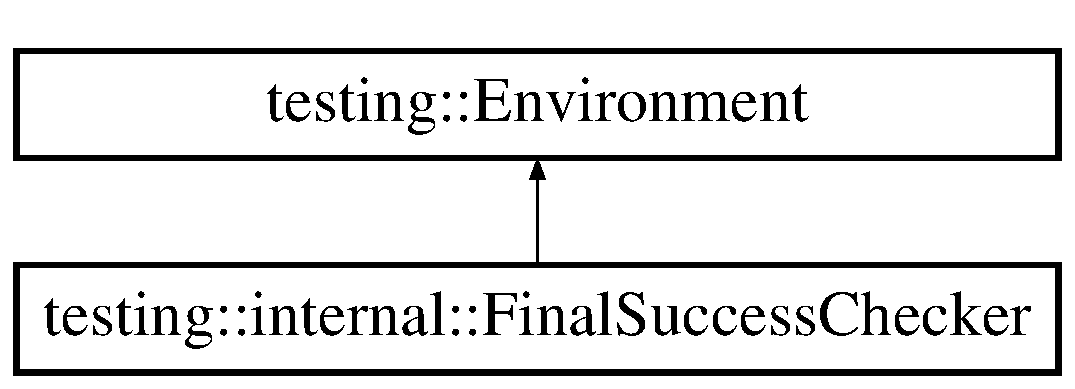
\includegraphics[height=2.000000cm]{classtesting_1_1internal_1_1_final_success_checker}
\end{center}
\end{figure}
\subsection*{Protected Member Functions}
\begin{DoxyCompactItemize}
\item 
\mbox{\Hypertarget{classtesting_1_1internal_1_1_final_success_checker_a8f39d12a1f2bfe8c6c04b5c6749382c9}\label{classtesting_1_1internal_1_1_final_success_checker_a8f39d12a1f2bfe8c6c04b5c6749382c9}} 
virtual void {\bfseries Tear\+Down} ()
\end{DoxyCompactItemize}
\subsection*{Additional Inherited Members}


The documentation for this class was generated from the following file\+:\begin{DoxyCompactItemize}
\item 
/\+Users/fjp/git/bachelor/bachelor-\/master\+\_\+updated\+\_\+vfinal/googletest-\/1.\+8.\+0/googletest/test/gtest-\/unittest-\/api\+\_\+test.\+cc\end{DoxyCompactItemize}

\hypertarget{structtesting_1_1_flags}{}\section{testing\+:\+:Flags Struct Reference}
\label{structtesting_1_1_flags}\index{testing\+::\+Flags@{testing\+::\+Flags}}
\subsection*{Static Public Member Functions}
\begin{DoxyCompactItemize}
\item 
\mbox{\Hypertarget{structtesting_1_1_flags_a8bee2b5f94d8248b6791d6b005db146f}\label{structtesting_1_1_flags_a8bee2b5f94d8248b6791d6b005db146f}} 
static \mbox{\hyperlink{structtesting_1_1_flags}{Flags}} {\bfseries Also\+Run\+Disabled\+Tests} (bool also\+\_\+run\+\_\+disabled\+\_\+tests)
\item 
\mbox{\Hypertarget{structtesting_1_1_flags_a62660e44922321f7640bc951a04c2296}\label{structtesting_1_1_flags_a62660e44922321f7640bc951a04c2296}} 
static \mbox{\hyperlink{structtesting_1_1_flags}{Flags}} {\bfseries Break\+On\+Failure} (bool break\+\_\+on\+\_\+failure)
\item 
\mbox{\Hypertarget{structtesting_1_1_flags_a2c7d89f62f4328ae0ced66154ef96b44}\label{structtesting_1_1_flags_a2c7d89f62f4328ae0ced66154ef96b44}} 
static \mbox{\hyperlink{structtesting_1_1_flags}{Flags}} {\bfseries Catch\+Exceptions} (bool catch\+\_\+exceptions)
\item 
\mbox{\Hypertarget{structtesting_1_1_flags_a4468e5625833043596c44be174349d8c}\label{structtesting_1_1_flags_a4468e5625833043596c44be174349d8c}} 
static \mbox{\hyperlink{structtesting_1_1_flags}{Flags}} {\bfseries Death\+Test\+Use\+Fork} (bool death\+\_\+test\+\_\+use\+\_\+fork)
\item 
\mbox{\Hypertarget{structtesting_1_1_flags_afc7350b7c1ac4c0e0efe2d9a94729eb7}\label{structtesting_1_1_flags_afc7350b7c1ac4c0e0efe2d9a94729eb7}} 
static \mbox{\hyperlink{structtesting_1_1_flags}{Flags}} {\bfseries Filter} (const char $\ast$filter)
\item 
\mbox{\Hypertarget{structtesting_1_1_flags_a825a5d763a31fe6c28f543990bd336df}\label{structtesting_1_1_flags_a825a5d763a31fe6c28f543990bd336df}} 
static \mbox{\hyperlink{structtesting_1_1_flags}{Flags}} {\bfseries List\+Tests} (bool list\+\_\+tests)
\item 
\mbox{\Hypertarget{structtesting_1_1_flags_a507916734a6d7ff2dd02891d7849f2d3}\label{structtesting_1_1_flags_a507916734a6d7ff2dd02891d7849f2d3}} 
static \mbox{\hyperlink{structtesting_1_1_flags}{Flags}} {\bfseries Output} (const char $\ast$output)
\item 
\mbox{\Hypertarget{structtesting_1_1_flags_af4dc8454995fb3691399a049e95de179}\label{structtesting_1_1_flags_af4dc8454995fb3691399a049e95de179}} 
static \mbox{\hyperlink{structtesting_1_1_flags}{Flags}} {\bfseries Print\+Time} (bool print\+\_\+time)
\item 
\mbox{\Hypertarget{structtesting_1_1_flags_a695cd8b8ab44df5eaa371bacded78c05}\label{structtesting_1_1_flags_a695cd8b8ab44df5eaa371bacded78c05}} 
static \mbox{\hyperlink{structtesting_1_1_flags}{Flags}} {\bfseries Random\+Seed} (Int32 random\+\_\+seed)
\item 
\mbox{\Hypertarget{structtesting_1_1_flags_a19d47e87d77a18ef4fa8a85b74e25956}\label{structtesting_1_1_flags_a19d47e87d77a18ef4fa8a85b74e25956}} 
static \mbox{\hyperlink{structtesting_1_1_flags}{Flags}} {\bfseries Repeat} (Int32 repeat)
\item 
\mbox{\Hypertarget{structtesting_1_1_flags_a19ddbbaed61bda44a1940333b7c5a469}\label{structtesting_1_1_flags_a19ddbbaed61bda44a1940333b7c5a469}} 
static \mbox{\hyperlink{structtesting_1_1_flags}{Flags}} {\bfseries Shuffle} (bool shuffle)
\item 
\mbox{\Hypertarget{structtesting_1_1_flags_a16b01d8bcceaa9fa8211fd24faa75b5a}\label{structtesting_1_1_flags_a16b01d8bcceaa9fa8211fd24faa75b5a}} 
static \mbox{\hyperlink{structtesting_1_1_flags}{Flags}} {\bfseries Stack\+Trace\+Depth} (Int32 stack\+\_\+trace\+\_\+depth)
\item 
\mbox{\Hypertarget{structtesting_1_1_flags_a9cf0f64310b28eadbbfbb35584ebfc71}\label{structtesting_1_1_flags_a9cf0f64310b28eadbbfbb35584ebfc71}} 
static \mbox{\hyperlink{structtesting_1_1_flags}{Flags}} {\bfseries Stream\+Result\+To} (const char $\ast$stream\+\_\+result\+\_\+to)
\item 
\mbox{\Hypertarget{structtesting_1_1_flags_ad856df862414ed0dadf80b5e03829cc7}\label{structtesting_1_1_flags_ad856df862414ed0dadf80b5e03829cc7}} 
static \mbox{\hyperlink{structtesting_1_1_flags}{Flags}} {\bfseries Throw\+On\+Failure} (bool throw\+\_\+on\+\_\+failure)
\end{DoxyCompactItemize}
\subsection*{Public Attributes}
\begin{DoxyCompactItemize}
\item 
\mbox{\Hypertarget{structtesting_1_1_flags_a8ebf8c68f918b9039926b569c880f910}\label{structtesting_1_1_flags_a8ebf8c68f918b9039926b569c880f910}} 
bool {\bfseries also\+\_\+run\+\_\+disabled\+\_\+tests}
\item 
\mbox{\Hypertarget{structtesting_1_1_flags_acccce2a9673bb61751269d2ef9c21c89}\label{structtesting_1_1_flags_acccce2a9673bb61751269d2ef9c21c89}} 
bool {\bfseries break\+\_\+on\+\_\+failure}
\item 
\mbox{\Hypertarget{structtesting_1_1_flags_a06984d0553f09716e1bd9f159e7cc644}\label{structtesting_1_1_flags_a06984d0553f09716e1bd9f159e7cc644}} 
bool {\bfseries catch\+\_\+exceptions}
\item 
\mbox{\Hypertarget{structtesting_1_1_flags_a7cdef4e6e102771fc15940931dd07e5c}\label{structtesting_1_1_flags_a7cdef4e6e102771fc15940931dd07e5c}} 
bool {\bfseries death\+\_\+test\+\_\+use\+\_\+fork}
\item 
\mbox{\Hypertarget{structtesting_1_1_flags_aa52c1048a7e3cbe726ed4160f2e05d14}\label{structtesting_1_1_flags_aa52c1048a7e3cbe726ed4160f2e05d14}} 
const char $\ast$ {\bfseries filter}
\item 
\mbox{\Hypertarget{structtesting_1_1_flags_a3c73f29131074146224018066379fb2f}\label{structtesting_1_1_flags_a3c73f29131074146224018066379fb2f}} 
bool {\bfseries list\+\_\+tests}
\item 
\mbox{\Hypertarget{structtesting_1_1_flags_a8c8289b3af9310744bc25280e3980e4b}\label{structtesting_1_1_flags_a8c8289b3af9310744bc25280e3980e4b}} 
const char $\ast$ {\bfseries output}
\item 
\mbox{\Hypertarget{structtesting_1_1_flags_a8758d574ce5513402679df258f788733}\label{structtesting_1_1_flags_a8758d574ce5513402679df258f788733}} 
bool {\bfseries print\+\_\+time}
\item 
\mbox{\Hypertarget{structtesting_1_1_flags_a4728bce63433f711205fd7b427e57f1b}\label{structtesting_1_1_flags_a4728bce63433f711205fd7b427e57f1b}} 
Int32 {\bfseries random\+\_\+seed}
\item 
\mbox{\Hypertarget{structtesting_1_1_flags_a61614dd07f97f6e04d27c004ff15195e}\label{structtesting_1_1_flags_a61614dd07f97f6e04d27c004ff15195e}} 
Int32 {\bfseries repeat}
\item 
\mbox{\Hypertarget{structtesting_1_1_flags_a51c689e47e0f55c16116ac2a1d3b05d6}\label{structtesting_1_1_flags_a51c689e47e0f55c16116ac2a1d3b05d6}} 
bool {\bfseries shuffle}
\item 
\mbox{\Hypertarget{structtesting_1_1_flags_a20c6592453909c1adace64bf6a2bc2de}\label{structtesting_1_1_flags_a20c6592453909c1adace64bf6a2bc2de}} 
Int32 {\bfseries stack\+\_\+trace\+\_\+depth}
\item 
\mbox{\Hypertarget{structtesting_1_1_flags_ab09849fd3e095d5628dec65ec4dce9e1}\label{structtesting_1_1_flags_ab09849fd3e095d5628dec65ec4dce9e1}} 
const char $\ast$ {\bfseries stream\+\_\+result\+\_\+to}
\item 
\mbox{\Hypertarget{structtesting_1_1_flags_ab8e7d21e31e641efe47b8050759e001a}\label{structtesting_1_1_flags_ab8e7d21e31e641efe47b8050759e001a}} 
bool {\bfseries throw\+\_\+on\+\_\+failure}
\end{DoxyCompactItemize}


The documentation for this struct was generated from the following file\+:\begin{DoxyCompactItemize}
\item 
/\+Users/fjp/git/bachelor/bachelor-\/master\+\_\+updated\+\_\+vfinal/googletest-\/1.\+8.\+0/googletest/test/gtest\+\_\+unittest.\+cc\end{DoxyCompactItemize}

\hypertarget{classtesting_1_1internal_1_1_floating_point}{}\section{testing\+:\+:internal\+:\+:Floating\+Point$<$ Raw\+Type $>$ Class Template Reference}
\label{classtesting_1_1internal_1_1_floating_point}\index{testing\+::internal\+::\+Floating\+Point$<$ Raw\+Type $>$@{testing\+::internal\+::\+Floating\+Point$<$ Raw\+Type $>$}}
\subsection*{Public Types}
\begin{DoxyCompactItemize}
\item 
\mbox{\Hypertarget{classtesting_1_1internal_1_1_floating_point_abf228bf6cd48f12c8b44c85b4971a731}\label{classtesting_1_1internal_1_1_floating_point_abf228bf6cd48f12c8b44c85b4971a731}} 
typedef \mbox{\hyperlink{classtesting_1_1internal_1_1_type_with_size}{Type\+With\+Size}}$<$ sizeof(Raw\+Type)$>$\+::U\+Int {\bfseries Bits}
\end{DoxyCompactItemize}
\subsection*{Public Member Functions}
\begin{DoxyCompactItemize}
\item 
\mbox{\Hypertarget{classtesting_1_1internal_1_1_floating_point_a0dabf840863e0df84046f171c891fe71}\label{classtesting_1_1internal_1_1_floating_point_a0dabf840863e0df84046f171c891fe71}} 
{\bfseries Floating\+Point} (const Raw\+Type \&x)
\item 
\mbox{\Hypertarget{classtesting_1_1internal_1_1_floating_point_aab053be914bdc9e507c0db89740c318c}\label{classtesting_1_1internal_1_1_floating_point_aab053be914bdc9e507c0db89740c318c}} 
const Bits \& {\bfseries bits} () const
\item 
\mbox{\Hypertarget{classtesting_1_1internal_1_1_floating_point_af6bf8fab8df572ecb137a3516ff390ae}\label{classtesting_1_1internal_1_1_floating_point_af6bf8fab8df572ecb137a3516ff390ae}} 
Bits {\bfseries exponent\+\_\+bits} () const
\item 
\mbox{\Hypertarget{classtesting_1_1internal_1_1_floating_point_aa17337e50a2ac855719bc0676529558f}\label{classtesting_1_1internal_1_1_floating_point_aa17337e50a2ac855719bc0676529558f}} 
Bits {\bfseries fraction\+\_\+bits} () const
\item 
\mbox{\Hypertarget{classtesting_1_1internal_1_1_floating_point_afb8a816bb598225d775caaf43a893ef0}\label{classtesting_1_1internal_1_1_floating_point_afb8a816bb598225d775caaf43a893ef0}} 
Bits {\bfseries sign\+\_\+bit} () const
\item 
\mbox{\Hypertarget{classtesting_1_1internal_1_1_floating_point_a1fc654fd206efa98e480aa1e034f30d5}\label{classtesting_1_1internal_1_1_floating_point_a1fc654fd206efa98e480aa1e034f30d5}} 
bool {\bfseries is\+\_\+nan} () const
\item 
\mbox{\Hypertarget{classtesting_1_1internal_1_1_floating_point_a965214c1af2f9ac5adb1393794aa81e5}\label{classtesting_1_1internal_1_1_floating_point_a965214c1af2f9ac5adb1393794aa81e5}} 
bool {\bfseries Almost\+Equals} (const \mbox{\hyperlink{classtesting_1_1internal_1_1_floating_point}{Floating\+Point}} \&rhs) const
\item 
\mbox{\Hypertarget{classtesting_1_1internal_1_1_floating_point_af2eda9331e679229a1baa3404b57b51d}\label{classtesting_1_1internal_1_1_floating_point_af2eda9331e679229a1baa3404b57b51d}} 
{\footnotesize template$<$$>$ }\\float {\bfseries Max} ()
\item 
\mbox{\Hypertarget{classtesting_1_1internal_1_1_floating_point_afc2e85c0e886cb13b2300e961c9a9648}\label{classtesting_1_1internal_1_1_floating_point_afc2e85c0e886cb13b2300e961c9a9648}} 
{\footnotesize template$<$$>$ }\\double {\bfseries Max} ()
\end{DoxyCompactItemize}
\subsection*{Static Public Member Functions}
\begin{DoxyCompactItemize}
\item 
\mbox{\Hypertarget{classtesting_1_1internal_1_1_floating_point_ac551f793522e54fbd8a25acb79eac5b1}\label{classtesting_1_1internal_1_1_floating_point_ac551f793522e54fbd8a25acb79eac5b1}} 
static Raw\+Type {\bfseries Reinterpret\+Bits} (const Bits bits)
\item 
\mbox{\Hypertarget{classtesting_1_1internal_1_1_floating_point_a460027cc19cf01ae8e09cc3796b2b575}\label{classtesting_1_1internal_1_1_floating_point_a460027cc19cf01ae8e09cc3796b2b575}} 
static Raw\+Type {\bfseries Infinity} ()
\item 
\mbox{\Hypertarget{classtesting_1_1internal_1_1_floating_point_aae5954d8a57d3ff0987c6930cb68e114}\label{classtesting_1_1internal_1_1_floating_point_aae5954d8a57d3ff0987c6930cb68e114}} 
static Raw\+Type {\bfseries Max} ()
\end{DoxyCompactItemize}
\subsection*{Static Public Attributes}
\begin{DoxyCompactItemize}
\item 
\mbox{\Hypertarget{classtesting_1_1internal_1_1_floating_point_ab819d2e8f93e9e482373999f0f8d71b9}\label{classtesting_1_1internal_1_1_floating_point_ab819d2e8f93e9e482373999f0f8d71b9}} 
static const size\+\_\+t {\bfseries k\+Bit\+Count} = 8$\ast$sizeof(Raw\+Type)
\item 
static const size\+\_\+t {\bfseries k\+Fraction\+Bit\+Count}
\item 
\mbox{\Hypertarget{classtesting_1_1internal_1_1_floating_point_a1973d843c00781053d3073daa8a40119}\label{classtesting_1_1internal_1_1_floating_point_a1973d843c00781053d3073daa8a40119}} 
static const size\+\_\+t {\bfseries k\+Exponent\+Bit\+Count} = k\+Bit\+Count -\/ 1 -\/ k\+Fraction\+Bit\+Count
\item 
\mbox{\Hypertarget{classtesting_1_1internal_1_1_floating_point_aca98b5ea6f2222a66a82e52421682efa}\label{classtesting_1_1internal_1_1_floating_point_aca98b5ea6f2222a66a82e52421682efa}} 
static const Bits {\bfseries k\+Sign\+Bit\+Mask} = static\+\_\+cast$<$Bits$>$(1) $<$$<$ (k\+Bit\+Count -\/ 1)
\item 
static const Bits {\bfseries k\+Fraction\+Bit\+Mask}
\item 
\mbox{\Hypertarget{classtesting_1_1internal_1_1_floating_point_a66065dfc4d5f41100f686159637af23b}\label{classtesting_1_1internal_1_1_floating_point_a66065dfc4d5f41100f686159637af23b}} 
static const Bits {\bfseries k\+Exponent\+Bit\+Mask} = $\sim$(k\+Sign\+Bit\+Mask $\vert$ k\+Fraction\+Bit\+Mask)
\item 
\mbox{\Hypertarget{classtesting_1_1internal_1_1_floating_point_aac498b3714d93f8e88cdc30e4c5935f6}\label{classtesting_1_1internal_1_1_floating_point_aac498b3714d93f8e88cdc30e4c5935f6}} 
static const size\+\_\+t {\bfseries k\+Max\+Ulps} = 4
\end{DoxyCompactItemize}


\subsection{Member Data Documentation}
\mbox{\Hypertarget{classtesting_1_1internal_1_1_floating_point_a0b756a6d2a4f5f5b41ca79651c06c043}\label{classtesting_1_1internal_1_1_floating_point_a0b756a6d2a4f5f5b41ca79651c06c043}} 
\index{testing\+::internal\+::\+Floating\+Point@{testing\+::internal\+::\+Floating\+Point}!k\+Fraction\+Bit\+Count@{k\+Fraction\+Bit\+Count}}
\index{k\+Fraction\+Bit\+Count@{k\+Fraction\+Bit\+Count}!testing\+::internal\+::\+Floating\+Point@{testing\+::internal\+::\+Floating\+Point}}
\subsubsection{\texorpdfstring{k\+Fraction\+Bit\+Count}{kFractionBitCount}}
{\footnotesize\ttfamily template$<$typename Raw\+Type $>$ \\
const size\+\_\+t \mbox{\hyperlink{classtesting_1_1internal_1_1_floating_point}{testing\+::internal\+::\+Floating\+Point}}$<$ Raw\+Type $>$\+::k\+Fraction\+Bit\+Count\hspace{0.3cm}{\ttfamily [static]}}

{\bfseries Initial value\+:}
\begin{DoxyCode}
=
    std::numeric\_limits<RawType>::digits - 1
\end{DoxyCode}
\mbox{\Hypertarget{classtesting_1_1internal_1_1_floating_point_a0ac75d4ffd24f14bca452abe8a718da1}\label{classtesting_1_1internal_1_1_floating_point_a0ac75d4ffd24f14bca452abe8a718da1}} 
\index{testing\+::internal\+::\+Floating\+Point@{testing\+::internal\+::\+Floating\+Point}!k\+Fraction\+Bit\+Mask@{k\+Fraction\+Bit\+Mask}}
\index{k\+Fraction\+Bit\+Mask@{k\+Fraction\+Bit\+Mask}!testing\+::internal\+::\+Floating\+Point@{testing\+::internal\+::\+Floating\+Point}}
\subsubsection{\texorpdfstring{k\+Fraction\+Bit\+Mask}{kFractionBitMask}}
{\footnotesize\ttfamily template$<$typename Raw\+Type $>$ \\
const Bits \mbox{\hyperlink{classtesting_1_1internal_1_1_floating_point}{testing\+::internal\+::\+Floating\+Point}}$<$ Raw\+Type $>$\+::k\+Fraction\+Bit\+Mask\hspace{0.3cm}{\ttfamily [static]}}

{\bfseries Initial value\+:}
\begin{DoxyCode}
=
    ~static\_cast<Bits>(0) >> (kExponentBitCount + 1)
\end{DoxyCode}


The documentation for this class was generated from the following file\+:\begin{DoxyCompactItemize}
\item 
/\+Users/fjp/git/bachelor/bachelor-\/master\+\_\+updated\+\_\+vfinal/googletest-\/1.\+8.\+0/googletest/include/gtest/internal/gtest-\/internal.\+h\end{DoxyCompactItemize}

\hypertarget{structtesting_1_1gtest__printers__test_1_1_foo}{}\section{testing\+:\+:gtest\+\_\+printers\+\_\+test\+:\+:Foo Struct Reference}
\label{structtesting_1_1gtest__printers__test_1_1_foo}\index{testing\+::gtest\+\_\+printers\+\_\+test\+::\+Foo@{testing\+::gtest\+\_\+printers\+\_\+test\+::\+Foo}}
\subsection*{Public Member Functions}
\begin{DoxyCompactItemize}
\item 
\mbox{\Hypertarget{structtesting_1_1gtest__printers__test_1_1_foo_a703c1159114f3a640b16d470a9613672}\label{structtesting_1_1gtest__printers__test_1_1_foo_a703c1159114f3a640b16d470a9613672}} 
int {\bfseries My\+Method} (char x)
\item 
\mbox{\Hypertarget{structtesting_1_1gtest__printers__test_1_1_foo_a368dc5150b27c2aaca6034830334e1cd}\label{structtesting_1_1gtest__printers__test_1_1_foo_a368dc5150b27c2aaca6034830334e1cd}} 
virtual char {\bfseries My\+Virtual\+Method} (int)
\end{DoxyCompactItemize}
\subsection*{Public Attributes}
\begin{DoxyCompactItemize}
\item 
\mbox{\Hypertarget{structtesting_1_1gtest__printers__test_1_1_foo_a8171a69191d34071ea4448d2dda501ec}\label{structtesting_1_1gtest__printers__test_1_1_foo_a8171a69191d34071ea4448d2dda501ec}} 
int {\bfseries value}
\end{DoxyCompactItemize}


The documentation for this struct was generated from the following file\+:\begin{DoxyCompactItemize}
\item 
/\+Users/fjp/git/bachelor/bachelor-\/master\+\_\+updated\+\_\+vfinal/googletest-\/1.\+8.\+0/googletest/test/gtest-\/printers\+\_\+test.\+cc\end{DoxyCompactItemize}

\hypertarget{class_foo_environment}{}\section{Foo\+Environment Class Reference}
\label{class_foo_environment}\index{Foo\+Environment@{Foo\+Environment}}
Inheritance diagram for Foo\+Environment\+:\begin{figure}[H]
\begin{center}
\leavevmode
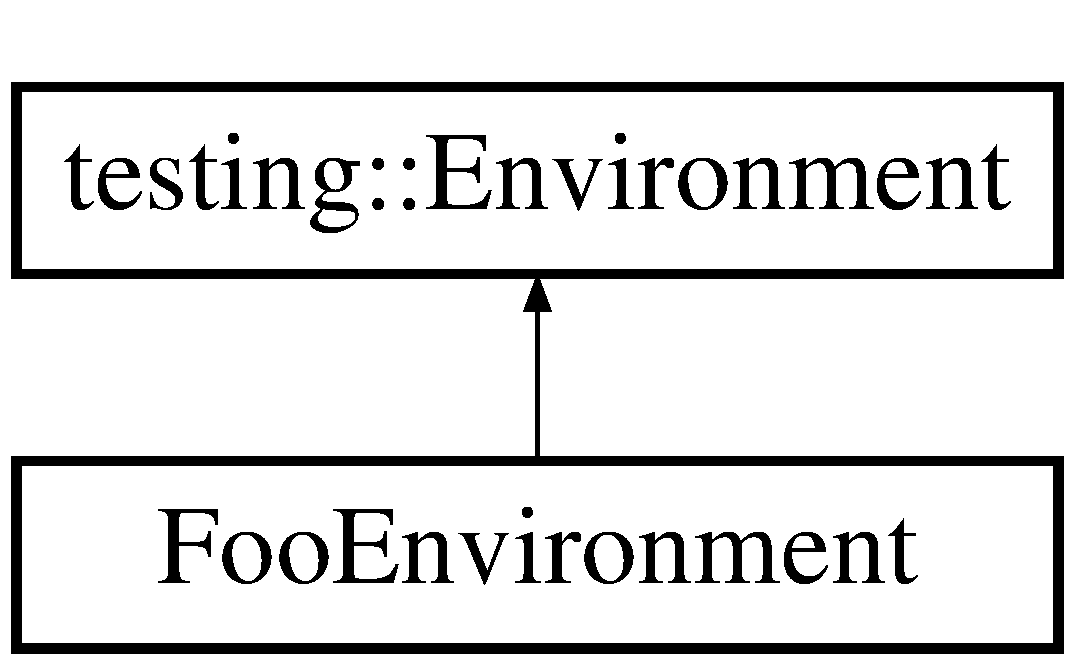
\includegraphics[height=2.000000cm]{class_foo_environment}
\end{center}
\end{figure}
\subsection*{Public Member Functions}
\begin{DoxyCompactItemize}
\item 
\mbox{\Hypertarget{class_foo_environment_a7db8d8b312805aff437ae8534132a56d}\label{class_foo_environment_a7db8d8b312805aff437ae8534132a56d}} 
virtual void {\bfseries Set\+Up} ()
\item 
\mbox{\Hypertarget{class_foo_environment_a99a2c9df52106cce9e7a4bdda53df802}\label{class_foo_environment_a99a2c9df52106cce9e7a4bdda53df802}} 
virtual void {\bfseries Tear\+Down} ()
\end{DoxyCompactItemize}


The documentation for this class was generated from the following file\+:\begin{DoxyCompactItemize}
\item 
/\+Users/fjp/git/bachelor/bachelor-\/master\+\_\+updated\+\_\+vfinal/googletest-\/1.\+8.\+0/googletest/test/gtest\+\_\+output\+\_\+test\+\_\+.\+cc\end{DoxyCompactItemize}

\hypertarget{class_foo_test}{}\section{Foo\+Test Class Reference}
\label{class_foo_test}\index{Foo\+Test@{Foo\+Test}}
Inheritance diagram for Foo\+Test\+:\begin{figure}[H]
\begin{center}
\leavevmode
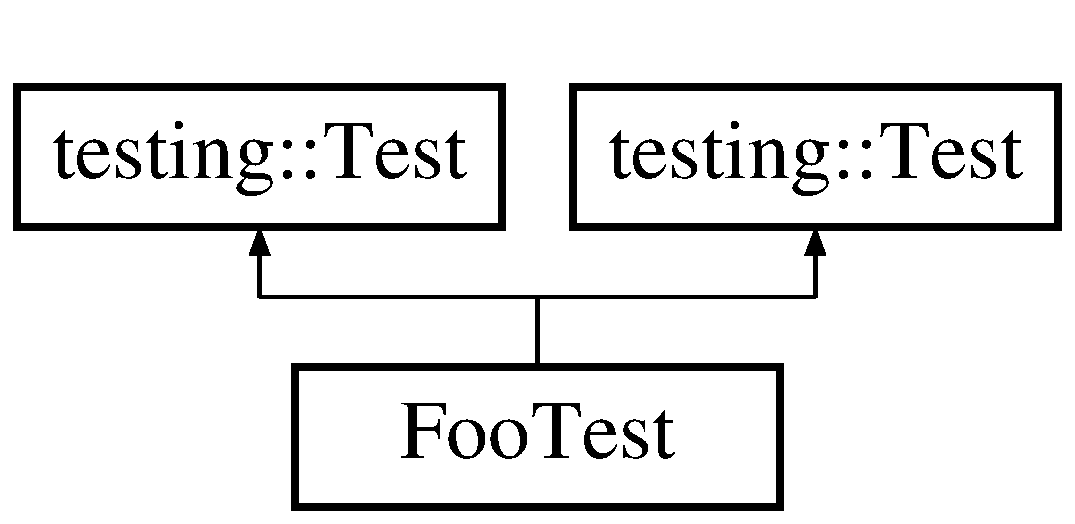
\includegraphics[height=2.000000cm]{class_foo_test}
\end{center}
\end{figure}
\subsection*{Additional Inherited Members}


The documentation for this class was generated from the following file\+:\begin{DoxyCompactItemize}
\item 
/\+Users/fjp/git/bachelor/bachelor-\/master\+\_\+updated\+\_\+vfinal/googletest-\/1.\+8.\+0/googletest/test/gtest\+\_\+list\+\_\+tests\+\_\+unittest\+\_\+.\+cc\end{DoxyCompactItemize}

\hypertarget{classtesting_1_1internal_1_1_format_for_comparison}{}\section{testing\+:\+:internal\+:\+:Format\+For\+Comparison$<$ To\+Print, Other\+Operand $>$ Class Template Reference}
\label{classtesting_1_1internal_1_1_format_for_comparison}\index{testing\+::internal\+::\+Format\+For\+Comparison$<$ To\+Print, Other\+Operand $>$@{testing\+::internal\+::\+Format\+For\+Comparison$<$ To\+Print, Other\+Operand $>$}}
\subsection*{Static Public Member Functions}
\begin{DoxyCompactItemize}
\item 
\mbox{\Hypertarget{classtesting_1_1internal_1_1_format_for_comparison_a2aeb688fc55b57abd3021d82eccad896}\label{classtesting_1_1internal_1_1_format_for_comparison_a2aeb688fc55b57abd3021d82eccad896}} 
\+::std\+::string {\bfseries Format} (const To\+Print \&value)
\end{DoxyCompactItemize}


The documentation for this class was generated from the following file\+:\begin{DoxyCompactItemize}
\item 
/\+Users/fjp/git/bachelor/bachelor-\/master\+\_\+updated\+\_\+vfinal/googletest-\/1.\+8.\+0/googletest/include/gtest/gtest-\/printers.\+h\end{DoxyCompactItemize}

\hypertarget{classtesting_1_1internal_1_1_format_for_comparison_3_01_to_print[_n]_00_01_other_operand_01_4}{}\section{testing\+:\+:internal\+:\+:Format\+For\+Comparison$<$ To\+Print\mbox{[}N\mbox{]}, Other\+Operand $>$ Class Template Reference}
\label{classtesting_1_1internal_1_1_format_for_comparison_3_01_to_print[_n]_00_01_other_operand_01_4}\index{testing\+::internal\+::\+Format\+For\+Comparison$<$ To\+Print\mbox{[}N\mbox{]}, Other\+Operand $>$@{testing\+::internal\+::\+Format\+For\+Comparison$<$ To\+Print[N], Other\+Operand $>$}}
\subsection*{Static Public Member Functions}
\begin{DoxyCompactItemize}
\item 
\mbox{\Hypertarget{classtesting_1_1internal_1_1_format_for_comparison_3_01_to_print[_n]_00_01_other_operand_01_4_a76c526461c8fa7df75f7b32ab889b9e0}\label{classtesting_1_1internal_1_1_format_for_comparison_3_01_to_print[_n]_00_01_other_operand_01_4_a76c526461c8fa7df75f7b32ab889b9e0}} 
\+::std\+::string {\bfseries Format} (const To\+Print $\ast$value)
\end{DoxyCompactItemize}


The documentation for this class was generated from the following file\+:\begin{DoxyCompactItemize}
\item 
/\+Users/fjp/git/bachelor/bachelor-\/master\+\_\+updated\+\_\+vfinal/googletest-\/1.\+8.\+0/googletest/include/gtest/gtest-\/printers.\+h\end{DoxyCompactItemize}

\hypertarget{classpump_1_1_for_node}{}\section{pump.\+For\+Node Class Reference}
\label{classpump_1_1_for_node}\index{pump.\+For\+Node@{pump.\+For\+Node}}
\subsection*{Public Member Functions}
\begin{DoxyCompactItemize}
\item 
\mbox{\Hypertarget{classpump_1_1_for_node_a9cf60468cacdb06acce35074ab2a2b55}\label{classpump_1_1_for_node_a9cf60468cacdb06acce35074ab2a2b55}} 
def {\bfseries \+\_\+\+\_\+init\+\_\+\+\_\+} (self, identifier=None, sep=None, code=None)
\end{DoxyCompactItemize}
\subsection*{Public Attributes}
\begin{DoxyCompactItemize}
\item 
\mbox{\Hypertarget{classpump_1_1_for_node_a2444199e135e43696b3a006bd0d38982}\label{classpump_1_1_for_node_a2444199e135e43696b3a006bd0d38982}} 
{\bfseries identifier}
\item 
\mbox{\Hypertarget{classpump_1_1_for_node_a06b493278b3c1ad53363a2bcc3b8efb3}\label{classpump_1_1_for_node_a06b493278b3c1ad53363a2bcc3b8efb3}} 
{\bfseries sep}
\item 
\mbox{\Hypertarget{classpump_1_1_for_node_afdb5f4f2a3bc772bbc6ea777dfde898e}\label{classpump_1_1_for_node_afdb5f4f2a3bc772bbc6ea777dfde898e}} 
{\bfseries code}
\end{DoxyCompactItemize}


The documentation for this class was generated from the following file\+:\begin{DoxyCompactItemize}
\item 
/\+Users/fjp/git/bachelor/bachelor-\/master\+\_\+updated\+\_\+vfinal/googletest-\/1.\+8.\+0/googletest/scripts/pump.\+py\end{DoxyCompactItemize}

\hypertarget{classstd_1_1tr1_1_1gtest__internal_1_1_get}{}\section{std\+:\+:tr1\+:\+:gtest\+\_\+internal\+:\+:Get$<$ k $>$ Class Template Reference}
\label{classstd_1_1tr1_1_1gtest__internal_1_1_get}\index{std\+::tr1\+::gtest\+\_\+internal\+::\+Get$<$ k $>$@{std\+::tr1\+::gtest\+\_\+internal\+::\+Get$<$ k $>$}}


The documentation for this class was generated from the following file\+:\begin{DoxyCompactItemize}
\item 
/\+Users/fjp/git/bachelor/bachelor-\/master\+\_\+updated\+\_\+vfinal/googletest-\/1.\+8.\+0/googletest/include/gtest/internal/gtest-\/tuple.\+h\end{DoxyCompactItemize}

\hypertarget{classstd_1_1tr1_1_1gtest__internal_1_1_get_3_010_01_4}{}\section{std\+:\+:tr1\+:\+:gtest\+\_\+internal\+:\+:Get$<$ 0 $>$ Class Template Reference}
\label{classstd_1_1tr1_1_1gtest__internal_1_1_get_3_010_01_4}\index{std\+::tr1\+::gtest\+\_\+internal\+::\+Get$<$ 0 $>$@{std\+::tr1\+::gtest\+\_\+internal\+::\+Get$<$ 0 $>$}}
\subsection*{Static Public Member Functions}
\begin{DoxyCompactItemize}
\item 
\mbox{\Hypertarget{classstd_1_1tr1_1_1gtest__internal_1_1_get_3_010_01_4_a74beca3869fddfe42ee608b7f4cacb96}\label{classstd_1_1tr1_1_1gtest__internal_1_1_get_3_010_01_4_a74beca3869fddfe42ee608b7f4cacb96}} 
{\footnotesize template$<$class Tuple $>$ }\\static {\bfseries G\+T\+E\+S\+T\+\_\+\+A\+D\+D\+\_\+\+R\+E\+F\+\_\+} (G\+T\+E\+S\+T\+\_\+\+T\+U\+P\+L\+E\+\_\+\+E\+L\+E\+M\+E\+N\+T\+\_\+(0, Tuple)) Field(Tuple \&t)
\item 
\mbox{\Hypertarget{classstd_1_1tr1_1_1gtest__internal_1_1_get_3_010_01_4_a195b3853de45077f9a324c455f22d7e2}\label{classstd_1_1tr1_1_1gtest__internal_1_1_get_3_010_01_4_a195b3853de45077f9a324c455f22d7e2}} 
{\footnotesize template$<$class Tuple $>$ }\\static {\bfseries G\+T\+E\+S\+T\+\_\+\+B\+Y\+\_\+\+R\+E\+F\+\_\+} (G\+T\+E\+S\+T\+\_\+\+T\+U\+P\+L\+E\+\_\+\+E\+L\+E\+M\+E\+N\+T\+\_\+(0, Tuple)) Const\+Field(const Tuple \&t)
\end{DoxyCompactItemize}


The documentation for this class was generated from the following file\+:\begin{DoxyCompactItemize}
\item 
/\+Users/fjp/git/bachelor/bachelor-\/master\+\_\+updated\+\_\+vfinal/googletest-\/1.\+8.\+0/googletest/include/gtest/internal/gtest-\/tuple.\+h\end{DoxyCompactItemize}

\hypertarget{classstd_1_1tr1_1_1gtest__internal_1_1_get_3_011_01_4}{}\section{std\+:\+:tr1\+:\+:gtest\+\_\+internal\+:\+:Get$<$ 1 $>$ Class Template Reference}
\label{classstd_1_1tr1_1_1gtest__internal_1_1_get_3_011_01_4}\index{std\+::tr1\+::gtest\+\_\+internal\+::\+Get$<$ 1 $>$@{std\+::tr1\+::gtest\+\_\+internal\+::\+Get$<$ 1 $>$}}
\subsection*{Static Public Member Functions}
\begin{DoxyCompactItemize}
\item 
\mbox{\Hypertarget{classstd_1_1tr1_1_1gtest__internal_1_1_get_3_011_01_4_a52b2f5d2bc283d76a3e8dede84dba154}\label{classstd_1_1tr1_1_1gtest__internal_1_1_get_3_011_01_4_a52b2f5d2bc283d76a3e8dede84dba154}} 
{\footnotesize template$<$class Tuple $>$ }\\static {\bfseries G\+T\+E\+S\+T\+\_\+\+A\+D\+D\+\_\+\+R\+E\+F\+\_\+} (G\+T\+E\+S\+T\+\_\+\+T\+U\+P\+L\+E\+\_\+\+E\+L\+E\+M\+E\+N\+T\+\_\+(1, Tuple)) Field(Tuple \&t)
\item 
\mbox{\Hypertarget{classstd_1_1tr1_1_1gtest__internal_1_1_get_3_011_01_4_a481a2bf839c758408d46a1d0d41ff8f4}\label{classstd_1_1tr1_1_1gtest__internal_1_1_get_3_011_01_4_a481a2bf839c758408d46a1d0d41ff8f4}} 
{\footnotesize template$<$class Tuple $>$ }\\static {\bfseries G\+T\+E\+S\+T\+\_\+\+B\+Y\+\_\+\+R\+E\+F\+\_\+} (G\+T\+E\+S\+T\+\_\+\+T\+U\+P\+L\+E\+\_\+\+E\+L\+E\+M\+E\+N\+T\+\_\+(1, Tuple)) Const\+Field(const Tuple \&t)
\end{DoxyCompactItemize}


The documentation for this class was generated from the following file\+:\begin{DoxyCompactItemize}
\item 
/\+Users/fjp/git/bachelor/bachelor-\/master\+\_\+updated\+\_\+vfinal/googletest-\/1.\+8.\+0/googletest/include/gtest/internal/gtest-\/tuple.\+h\end{DoxyCompactItemize}

\hypertarget{classstd_1_1tr1_1_1gtest__internal_1_1_get_3_012_01_4}{}\section{std\+:\+:tr1\+:\+:gtest\+\_\+internal\+:\+:Get$<$ 2 $>$ Class Template Reference}
\label{classstd_1_1tr1_1_1gtest__internal_1_1_get_3_012_01_4}\index{std\+::tr1\+::gtest\+\_\+internal\+::\+Get$<$ 2 $>$@{std\+::tr1\+::gtest\+\_\+internal\+::\+Get$<$ 2 $>$}}
\subsection*{Static Public Member Functions}
\begin{DoxyCompactItemize}
\item 
\mbox{\Hypertarget{classstd_1_1tr1_1_1gtest__internal_1_1_get_3_012_01_4_a8dfe7b5c1c915f10181e3fb5952ba6d8}\label{classstd_1_1tr1_1_1gtest__internal_1_1_get_3_012_01_4_a8dfe7b5c1c915f10181e3fb5952ba6d8}} 
{\footnotesize template$<$class Tuple $>$ }\\static {\bfseries G\+T\+E\+S\+T\+\_\+\+A\+D\+D\+\_\+\+R\+E\+F\+\_\+} (G\+T\+E\+S\+T\+\_\+\+T\+U\+P\+L\+E\+\_\+\+E\+L\+E\+M\+E\+N\+T\+\_\+(2, Tuple)) Field(Tuple \&t)
\item 
\mbox{\Hypertarget{classstd_1_1tr1_1_1gtest__internal_1_1_get_3_012_01_4_a76127c9c03c1f0caa61fb87d4d756b5b}\label{classstd_1_1tr1_1_1gtest__internal_1_1_get_3_012_01_4_a76127c9c03c1f0caa61fb87d4d756b5b}} 
{\footnotesize template$<$class Tuple $>$ }\\static {\bfseries G\+T\+E\+S\+T\+\_\+\+B\+Y\+\_\+\+R\+E\+F\+\_\+} (G\+T\+E\+S\+T\+\_\+\+T\+U\+P\+L\+E\+\_\+\+E\+L\+E\+M\+E\+N\+T\+\_\+(2, Tuple)) Const\+Field(const Tuple \&t)
\end{DoxyCompactItemize}


The documentation for this class was generated from the following file\+:\begin{DoxyCompactItemize}
\item 
/\+Users/fjp/git/bachelor/bachelor-\/master\+\_\+updated\+\_\+vfinal/googletest-\/1.\+8.\+0/googletest/include/gtest/internal/gtest-\/tuple.\+h\end{DoxyCompactItemize}

\hypertarget{classstd_1_1tr1_1_1gtest__internal_1_1_get_3_013_01_4}{}\section{std\+:\+:tr1\+:\+:gtest\+\_\+internal\+:\+:Get$<$ 3 $>$ Class Template Reference}
\label{classstd_1_1tr1_1_1gtest__internal_1_1_get_3_013_01_4}\index{std\+::tr1\+::gtest\+\_\+internal\+::\+Get$<$ 3 $>$@{std\+::tr1\+::gtest\+\_\+internal\+::\+Get$<$ 3 $>$}}
\subsection*{Static Public Member Functions}
\begin{DoxyCompactItemize}
\item 
\mbox{\Hypertarget{classstd_1_1tr1_1_1gtest__internal_1_1_get_3_013_01_4_aa2ebd71eca812f06bad0773a7e2f6788}\label{classstd_1_1tr1_1_1gtest__internal_1_1_get_3_013_01_4_aa2ebd71eca812f06bad0773a7e2f6788}} 
{\footnotesize template$<$class Tuple $>$ }\\static {\bfseries G\+T\+E\+S\+T\+\_\+\+A\+D\+D\+\_\+\+R\+E\+F\+\_\+} (G\+T\+E\+S\+T\+\_\+\+T\+U\+P\+L\+E\+\_\+\+E\+L\+E\+M\+E\+N\+T\+\_\+(3, Tuple)) Field(Tuple \&t)
\item 
\mbox{\Hypertarget{classstd_1_1tr1_1_1gtest__internal_1_1_get_3_013_01_4_ab8c5283e6776308abc41aaad518a23c7}\label{classstd_1_1tr1_1_1gtest__internal_1_1_get_3_013_01_4_ab8c5283e6776308abc41aaad518a23c7}} 
{\footnotesize template$<$class Tuple $>$ }\\static {\bfseries G\+T\+E\+S\+T\+\_\+\+B\+Y\+\_\+\+R\+E\+F\+\_\+} (G\+T\+E\+S\+T\+\_\+\+T\+U\+P\+L\+E\+\_\+\+E\+L\+E\+M\+E\+N\+T\+\_\+(3, Tuple)) Const\+Field(const Tuple \&t)
\end{DoxyCompactItemize}


The documentation for this class was generated from the following file\+:\begin{DoxyCompactItemize}
\item 
/\+Users/fjp/git/bachelor/bachelor-\/master\+\_\+updated\+\_\+vfinal/googletest-\/1.\+8.\+0/googletest/include/gtest/internal/gtest-\/tuple.\+h\end{DoxyCompactItemize}

\hypertarget{classstd_1_1tr1_1_1gtest__internal_1_1_get_3_014_01_4}{}\section{std\+:\+:tr1\+:\+:gtest\+\_\+internal\+:\+:Get$<$ 4 $>$ Class Template Reference}
\label{classstd_1_1tr1_1_1gtest__internal_1_1_get_3_014_01_4}\index{std\+::tr1\+::gtest\+\_\+internal\+::\+Get$<$ 4 $>$@{std\+::tr1\+::gtest\+\_\+internal\+::\+Get$<$ 4 $>$}}
\subsection*{Static Public Member Functions}
\begin{DoxyCompactItemize}
\item 
\mbox{\Hypertarget{classstd_1_1tr1_1_1gtest__internal_1_1_get_3_014_01_4_a5c7a91c681118bb7253e305f8ff42be4}\label{classstd_1_1tr1_1_1gtest__internal_1_1_get_3_014_01_4_a5c7a91c681118bb7253e305f8ff42be4}} 
{\footnotesize template$<$class Tuple $>$ }\\static {\bfseries G\+T\+E\+S\+T\+\_\+\+A\+D\+D\+\_\+\+R\+E\+F\+\_\+} (G\+T\+E\+S\+T\+\_\+\+T\+U\+P\+L\+E\+\_\+\+E\+L\+E\+M\+E\+N\+T\+\_\+(4, Tuple)) Field(Tuple \&t)
\item 
\mbox{\Hypertarget{classstd_1_1tr1_1_1gtest__internal_1_1_get_3_014_01_4_a04794c398bbe81e4de0915b79da2166a}\label{classstd_1_1tr1_1_1gtest__internal_1_1_get_3_014_01_4_a04794c398bbe81e4de0915b79da2166a}} 
{\footnotesize template$<$class Tuple $>$ }\\static {\bfseries G\+T\+E\+S\+T\+\_\+\+B\+Y\+\_\+\+R\+E\+F\+\_\+} (G\+T\+E\+S\+T\+\_\+\+T\+U\+P\+L\+E\+\_\+\+E\+L\+E\+M\+E\+N\+T\+\_\+(4, Tuple)) Const\+Field(const Tuple \&t)
\end{DoxyCompactItemize}


The documentation for this class was generated from the following file\+:\begin{DoxyCompactItemize}
\item 
/\+Users/fjp/git/bachelor/bachelor-\/master\+\_\+updated\+\_\+vfinal/googletest-\/1.\+8.\+0/googletest/include/gtest/internal/gtest-\/tuple.\+h\end{DoxyCompactItemize}

\hypertarget{classstd_1_1tr1_1_1gtest__internal_1_1_get_3_015_01_4}{}\section{std\+:\+:tr1\+:\+:gtest\+\_\+internal\+:\+:Get$<$ 5 $>$ Class Template Reference}
\label{classstd_1_1tr1_1_1gtest__internal_1_1_get_3_015_01_4}\index{std\+::tr1\+::gtest\+\_\+internal\+::\+Get$<$ 5 $>$@{std\+::tr1\+::gtest\+\_\+internal\+::\+Get$<$ 5 $>$}}
\subsection*{Static Public Member Functions}
\begin{DoxyCompactItemize}
\item 
\mbox{\Hypertarget{classstd_1_1tr1_1_1gtest__internal_1_1_get_3_015_01_4_a0a337088bab3f824f67d1607229fdcc2}\label{classstd_1_1tr1_1_1gtest__internal_1_1_get_3_015_01_4_a0a337088bab3f824f67d1607229fdcc2}} 
{\footnotesize template$<$class Tuple $>$ }\\static {\bfseries G\+T\+E\+S\+T\+\_\+\+A\+D\+D\+\_\+\+R\+E\+F\+\_\+} (G\+T\+E\+S\+T\+\_\+\+T\+U\+P\+L\+E\+\_\+\+E\+L\+E\+M\+E\+N\+T\+\_\+(5, Tuple)) Field(Tuple \&t)
\item 
\mbox{\Hypertarget{classstd_1_1tr1_1_1gtest__internal_1_1_get_3_015_01_4_ae10fe16450db82d69b9a4d0b149ca75d}\label{classstd_1_1tr1_1_1gtest__internal_1_1_get_3_015_01_4_ae10fe16450db82d69b9a4d0b149ca75d}} 
{\footnotesize template$<$class Tuple $>$ }\\static {\bfseries G\+T\+E\+S\+T\+\_\+\+B\+Y\+\_\+\+R\+E\+F\+\_\+} (G\+T\+E\+S\+T\+\_\+\+T\+U\+P\+L\+E\+\_\+\+E\+L\+E\+M\+E\+N\+T\+\_\+(5, Tuple)) Const\+Field(const Tuple \&t)
\end{DoxyCompactItemize}


The documentation for this class was generated from the following file\+:\begin{DoxyCompactItemize}
\item 
/\+Users/fjp/git/bachelor/bachelor-\/master\+\_\+updated\+\_\+vfinal/googletest-\/1.\+8.\+0/googletest/include/gtest/internal/gtest-\/tuple.\+h\end{DoxyCompactItemize}

\hypertarget{classstd_1_1tr1_1_1gtest__internal_1_1_get_3_016_01_4}{}\section{std\+:\+:tr1\+:\+:gtest\+\_\+internal\+:\+:Get$<$ 6 $>$ Class Template Reference}
\label{classstd_1_1tr1_1_1gtest__internal_1_1_get_3_016_01_4}\index{std\+::tr1\+::gtest\+\_\+internal\+::\+Get$<$ 6 $>$@{std\+::tr1\+::gtest\+\_\+internal\+::\+Get$<$ 6 $>$}}
\subsection*{Static Public Member Functions}
\begin{DoxyCompactItemize}
\item 
\mbox{\Hypertarget{classstd_1_1tr1_1_1gtest__internal_1_1_get_3_016_01_4_a28034152d066c8644fa55e9fc0e3a12d}\label{classstd_1_1tr1_1_1gtest__internal_1_1_get_3_016_01_4_a28034152d066c8644fa55e9fc0e3a12d}} 
{\footnotesize template$<$class Tuple $>$ }\\static {\bfseries G\+T\+E\+S\+T\+\_\+\+A\+D\+D\+\_\+\+R\+E\+F\+\_\+} (G\+T\+E\+S\+T\+\_\+\+T\+U\+P\+L\+E\+\_\+\+E\+L\+E\+M\+E\+N\+T\+\_\+(6, Tuple)) Field(Tuple \&t)
\item 
\mbox{\Hypertarget{classstd_1_1tr1_1_1gtest__internal_1_1_get_3_016_01_4_a6e396b998757e0ab9b75db0c68a7c360}\label{classstd_1_1tr1_1_1gtest__internal_1_1_get_3_016_01_4_a6e396b998757e0ab9b75db0c68a7c360}} 
{\footnotesize template$<$class Tuple $>$ }\\static {\bfseries G\+T\+E\+S\+T\+\_\+\+B\+Y\+\_\+\+R\+E\+F\+\_\+} (G\+T\+E\+S\+T\+\_\+\+T\+U\+P\+L\+E\+\_\+\+E\+L\+E\+M\+E\+N\+T\+\_\+(6, Tuple)) Const\+Field(const Tuple \&t)
\end{DoxyCompactItemize}


The documentation for this class was generated from the following file\+:\begin{DoxyCompactItemize}
\item 
/\+Users/fjp/git/bachelor/bachelor-\/master\+\_\+updated\+\_\+vfinal/googletest-\/1.\+8.\+0/googletest/include/gtest/internal/gtest-\/tuple.\+h\end{DoxyCompactItemize}

\hypertarget{classstd_1_1tr1_1_1gtest__internal_1_1_get_3_017_01_4}{}\section{std\+:\+:tr1\+:\+:gtest\+\_\+internal\+:\+:Get$<$ 7 $>$ Class Template Reference}
\label{classstd_1_1tr1_1_1gtest__internal_1_1_get_3_017_01_4}\index{std\+::tr1\+::gtest\+\_\+internal\+::\+Get$<$ 7 $>$@{std\+::tr1\+::gtest\+\_\+internal\+::\+Get$<$ 7 $>$}}
\subsection*{Static Public Member Functions}
\begin{DoxyCompactItemize}
\item 
\mbox{\Hypertarget{classstd_1_1tr1_1_1gtest__internal_1_1_get_3_017_01_4_ae1245f00b2ad610a130681b5bc81051c}\label{classstd_1_1tr1_1_1gtest__internal_1_1_get_3_017_01_4_ae1245f00b2ad610a130681b5bc81051c}} 
{\footnotesize template$<$class Tuple $>$ }\\static {\bfseries G\+T\+E\+S\+T\+\_\+\+A\+D\+D\+\_\+\+R\+E\+F\+\_\+} (G\+T\+E\+S\+T\+\_\+\+T\+U\+P\+L\+E\+\_\+\+E\+L\+E\+M\+E\+N\+T\+\_\+(7, Tuple)) Field(Tuple \&t)
\item 
\mbox{\Hypertarget{classstd_1_1tr1_1_1gtest__internal_1_1_get_3_017_01_4_afb7bd56e0697304325cd157d11df4a7b}\label{classstd_1_1tr1_1_1gtest__internal_1_1_get_3_017_01_4_afb7bd56e0697304325cd157d11df4a7b}} 
{\footnotesize template$<$class Tuple $>$ }\\static {\bfseries G\+T\+E\+S\+T\+\_\+\+B\+Y\+\_\+\+R\+E\+F\+\_\+} (G\+T\+E\+S\+T\+\_\+\+T\+U\+P\+L\+E\+\_\+\+E\+L\+E\+M\+E\+N\+T\+\_\+(7, Tuple)) Const\+Field(const Tuple \&t)
\end{DoxyCompactItemize}


The documentation for this class was generated from the following file\+:\begin{DoxyCompactItemize}
\item 
/\+Users/fjp/git/bachelor/bachelor-\/master\+\_\+updated\+\_\+vfinal/googletest-\/1.\+8.\+0/googletest/include/gtest/internal/gtest-\/tuple.\+h\end{DoxyCompactItemize}

\hypertarget{classstd_1_1tr1_1_1gtest__internal_1_1_get_3_018_01_4}{}\section{std\+:\+:tr1\+:\+:gtest\+\_\+internal\+:\+:Get$<$ 8 $>$ Class Template Reference}
\label{classstd_1_1tr1_1_1gtest__internal_1_1_get_3_018_01_4}\index{std\+::tr1\+::gtest\+\_\+internal\+::\+Get$<$ 8 $>$@{std\+::tr1\+::gtest\+\_\+internal\+::\+Get$<$ 8 $>$}}
\subsection*{Static Public Member Functions}
\begin{DoxyCompactItemize}
\item 
\mbox{\Hypertarget{classstd_1_1tr1_1_1gtest__internal_1_1_get_3_018_01_4_adf667300b7efed278f4ee3bf4d2edb85}\label{classstd_1_1tr1_1_1gtest__internal_1_1_get_3_018_01_4_adf667300b7efed278f4ee3bf4d2edb85}} 
{\footnotesize template$<$class Tuple $>$ }\\static {\bfseries G\+T\+E\+S\+T\+\_\+\+A\+D\+D\+\_\+\+R\+E\+F\+\_\+} (G\+T\+E\+S\+T\+\_\+\+T\+U\+P\+L\+E\+\_\+\+E\+L\+E\+M\+E\+N\+T\+\_\+(8, Tuple)) Field(Tuple \&t)
\item 
\mbox{\Hypertarget{classstd_1_1tr1_1_1gtest__internal_1_1_get_3_018_01_4_ab9645513ad2f983157f4062c89e910e7}\label{classstd_1_1tr1_1_1gtest__internal_1_1_get_3_018_01_4_ab9645513ad2f983157f4062c89e910e7}} 
{\footnotesize template$<$class Tuple $>$ }\\static {\bfseries G\+T\+E\+S\+T\+\_\+\+B\+Y\+\_\+\+R\+E\+F\+\_\+} (G\+T\+E\+S\+T\+\_\+\+T\+U\+P\+L\+E\+\_\+\+E\+L\+E\+M\+E\+N\+T\+\_\+(8, Tuple)) Const\+Field(const Tuple \&t)
\end{DoxyCompactItemize}


The documentation for this class was generated from the following file\+:\begin{DoxyCompactItemize}
\item 
/\+Users/fjp/git/bachelor/bachelor-\/master\+\_\+updated\+\_\+vfinal/googletest-\/1.\+8.\+0/googletest/include/gtest/internal/gtest-\/tuple.\+h\end{DoxyCompactItemize}

\hypertarget{classstd_1_1tr1_1_1gtest__internal_1_1_get_3_019_01_4}{}\section{std\+:\+:tr1\+:\+:gtest\+\_\+internal\+:\+:Get$<$ 9 $>$ Class Template Reference}
\label{classstd_1_1tr1_1_1gtest__internal_1_1_get_3_019_01_4}\index{std\+::tr1\+::gtest\+\_\+internal\+::\+Get$<$ 9 $>$@{std\+::tr1\+::gtest\+\_\+internal\+::\+Get$<$ 9 $>$}}
\subsection*{Static Public Member Functions}
\begin{DoxyCompactItemize}
\item 
\mbox{\Hypertarget{classstd_1_1tr1_1_1gtest__internal_1_1_get_3_019_01_4_add31197dfdb381d265e221ed62129f45}\label{classstd_1_1tr1_1_1gtest__internal_1_1_get_3_019_01_4_add31197dfdb381d265e221ed62129f45}} 
{\footnotesize template$<$class Tuple $>$ }\\static {\bfseries G\+T\+E\+S\+T\+\_\+\+A\+D\+D\+\_\+\+R\+E\+F\+\_\+} (G\+T\+E\+S\+T\+\_\+\+T\+U\+P\+L\+E\+\_\+\+E\+L\+E\+M\+E\+N\+T\+\_\+(9, Tuple)) Field(Tuple \&t)
\item 
\mbox{\Hypertarget{classstd_1_1tr1_1_1gtest__internal_1_1_get_3_019_01_4_a5205e8da729e2bee446f5be0c65390af}\label{classstd_1_1tr1_1_1gtest__internal_1_1_get_3_019_01_4_a5205e8da729e2bee446f5be0c65390af}} 
{\footnotesize template$<$class Tuple $>$ }\\static {\bfseries G\+T\+E\+S\+T\+\_\+\+B\+Y\+\_\+\+R\+E\+F\+\_\+} (G\+T\+E\+S\+T\+\_\+\+T\+U\+P\+L\+E\+\_\+\+E\+L\+E\+M\+E\+N\+T\+\_\+(9, Tuple)) Const\+Field(const Tuple \&t)
\end{DoxyCompactItemize}


The documentation for this class was generated from the following file\+:\begin{DoxyCompactItemize}
\item 
/\+Users/fjp/git/bachelor/bachelor-\/master\+\_\+updated\+\_\+vfinal/googletest-\/1.\+8.\+0/googletest/include/gtest/internal/gtest-\/tuple.\+h\end{DoxyCompactItemize}

\hypertarget{classupload_1_1_git_v_c_s}{}\section{upload.\+Git\+V\+CS Class Reference}
\label{classupload_1_1_git_v_c_s}\index{upload.\+Git\+V\+CS@{upload.\+Git\+V\+CS}}
Inheritance diagram for upload.\+Git\+V\+CS\+:\begin{figure}[H]
\begin{center}
\leavevmode
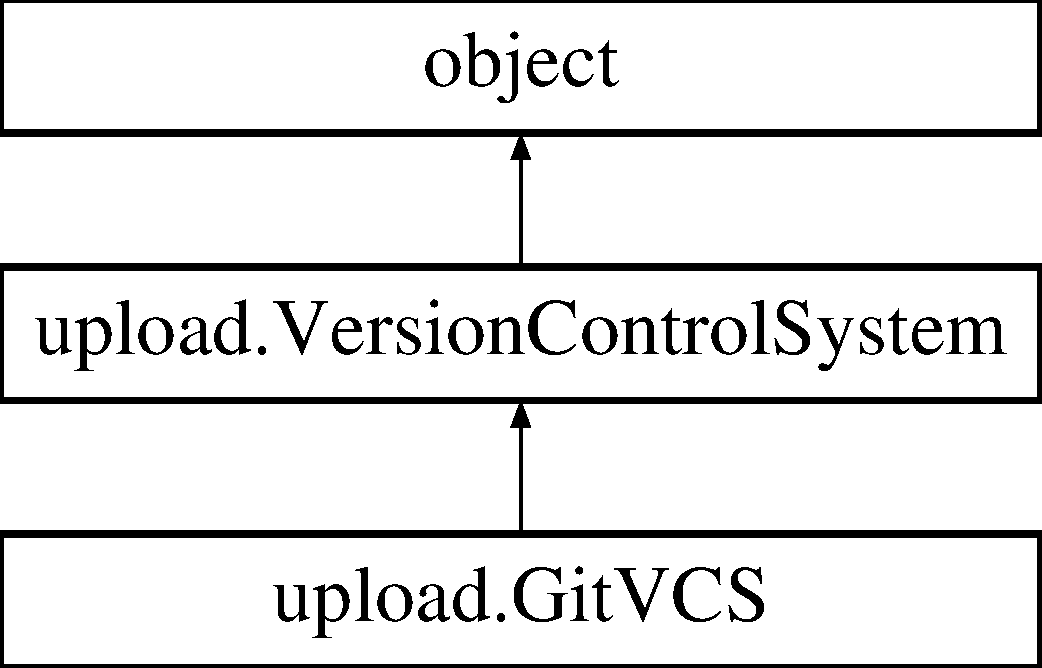
\includegraphics[height=3.000000cm]{classupload_1_1_git_v_c_s}
\end{center}
\end{figure}
\subsection*{Public Member Functions}
\begin{DoxyCompactItemize}
\item 
\mbox{\Hypertarget{classupload_1_1_git_v_c_s_aba4e1dca1c4b3e5db7ba07f6bce3c839}\label{classupload_1_1_git_v_c_s_aba4e1dca1c4b3e5db7ba07f6bce3c839}} 
def {\bfseries \+\_\+\+\_\+init\+\_\+\+\_\+} (self, options)
\item 
\mbox{\Hypertarget{classupload_1_1_git_v_c_s_a3ebfc01cebc9b585706ad3f4389a8833}\label{classupload_1_1_git_v_c_s_a3ebfc01cebc9b585706ad3f4389a8833}} 
def {\bfseries Generate\+Diff} (self, extra\+\_\+args)
\item 
\mbox{\Hypertarget{classupload_1_1_git_v_c_s_ae4e8c0e9fa01619c6a5c76d1ab84b995}\label{classupload_1_1_git_v_c_s_ae4e8c0e9fa01619c6a5c76d1ab84b995}} 
def {\bfseries Get\+Unknown\+Files} (self)
\item 
\mbox{\Hypertarget{classupload_1_1_git_v_c_s_a70ddb65a6b512b8cb8cc4affa37ff9b4}\label{classupload_1_1_git_v_c_s_a70ddb65a6b512b8cb8cc4affa37ff9b4}} 
def {\bfseries Get\+Base\+File} (self, filename)
\end{DoxyCompactItemize}
\subsection*{Public Attributes}
\begin{DoxyCompactItemize}
\item 
\mbox{\Hypertarget{classupload_1_1_git_v_c_s_a07e9469050a157f34fe804cdf6ecddac}\label{classupload_1_1_git_v_c_s_a07e9469050a157f34fe804cdf6ecddac}} 
{\bfseries base\+\_\+hashes}
\end{DoxyCompactItemize}


\subsection{Detailed Description}
\begin{DoxyVerb}Implementation of the VersionControlSystem interface for Git.\end{DoxyVerb}
 

The documentation for this class was generated from the following file\+:\begin{DoxyCompactItemize}
\item 
/\+Users/fjp/git/bachelor/bachelor-\/master\+\_\+updated\+\_\+vfinal/googletest-\/1.\+8.\+0/googletest/scripts/upload.\+py\end{DoxyCompactItemize}

\hypertarget{classgtest__break__on__failure__unittest_1_1_g_test_break_on_failure_unit_test}{}\section{gtest\+\_\+break\+\_\+on\+\_\+failure\+\_\+unittest.\+G\+Test\+Break\+On\+Failure\+Unit\+Test Class Reference}
\label{classgtest__break__on__failure__unittest_1_1_g_test_break_on_failure_unit_test}\index{gtest\+\_\+break\+\_\+on\+\_\+failure\+\_\+unittest.\+G\+Test\+Break\+On\+Failure\+Unit\+Test@{gtest\+\_\+break\+\_\+on\+\_\+failure\+\_\+unittest.\+G\+Test\+Break\+On\+Failure\+Unit\+Test}}
Inheritance diagram for gtest\+\_\+break\+\_\+on\+\_\+failure\+\_\+unittest.\+G\+Test\+Break\+On\+Failure\+Unit\+Test\+:\begin{figure}[H]
\begin{center}
\leavevmode
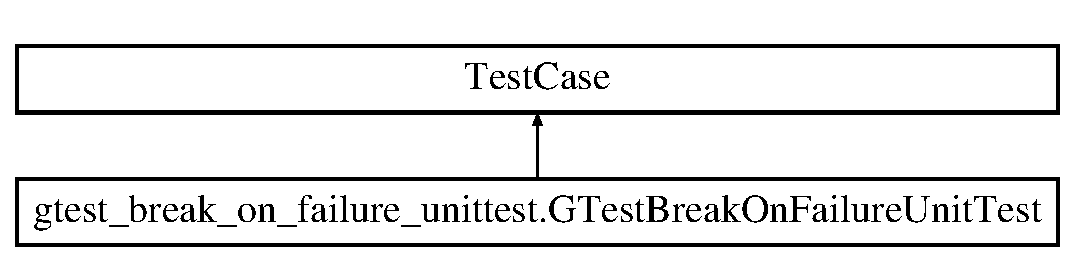
\includegraphics[height=2.000000cm]{classgtest__break__on__failure__unittest_1_1_g_test_break_on_failure_unit_test}
\end{center}
\end{figure}
\subsection*{Public Member Functions}
\begin{DoxyCompactItemize}
\item 
def \mbox{\hyperlink{classgtest__break__on__failure__unittest_1_1_g_test_break_on_failure_unit_test_a0a66475873f545d88655b8bb14368f2e}{Run\+And\+Verify}} (self, env\+\_\+var\+\_\+value, flag\+\_\+value, expect\+\_\+seg\+\_\+fault)
\item 
def \mbox{\hyperlink{classgtest__break__on__failure__unittest_1_1_g_test_break_on_failure_unit_test_a8c21b7ecccc27268cb6c3d30b933b812}{test\+Default\+Behavior}} (self)
\item 
def \mbox{\hyperlink{classgtest__break__on__failure__unittest_1_1_g_test_break_on_failure_unit_test_a2beae948940a4fd898c8183c3bb221da}{test\+Env\+Var}} (self)
\item 
def \mbox{\hyperlink{classgtest__break__on__failure__unittest_1_1_g_test_break_on_failure_unit_test_af6018e5253c1107c5afaba3e2cb573fe}{test\+Flag}} (self)
\item 
def \mbox{\hyperlink{classgtest__break__on__failure__unittest_1_1_g_test_break_on_failure_unit_test_a15836ddb27e51e9aaf2f8aad84f5cef7}{test\+Flag\+Overrides\+Env\+Var}} (self)
\item 
def \mbox{\hyperlink{classgtest__break__on__failure__unittest_1_1_g_test_break_on_failure_unit_test_a3c5855e045236a309a5bff73ee6b503e}{test\+Break\+On\+Failure\+Overrides\+Throw\+On\+Failure}} (self)
\item 
def \mbox{\hyperlink{classgtest__break__on__failure__unittest_1_1_g_test_break_on_failure_unit_test_a70cc7732ac68ffe587657a3a5309aa4a}{test\+Catch\+Exceptions\+Does\+Not\+Interfere}} (self)
\end{DoxyCompactItemize}


\subsection{Detailed Description}
\begin{DoxyVerb}Tests using the GTEST_BREAK_ON_FAILURE environment variable or
the --gtest_break_on_failure flag to turn assertion failures into
segmentation faults.
\end{DoxyVerb}
 

\subsection{Member Function Documentation}
\mbox{\Hypertarget{classgtest__break__on__failure__unittest_1_1_g_test_break_on_failure_unit_test_a0a66475873f545d88655b8bb14368f2e}\label{classgtest__break__on__failure__unittest_1_1_g_test_break_on_failure_unit_test_a0a66475873f545d88655b8bb14368f2e}} 
\index{gtest\+\_\+break\+\_\+on\+\_\+failure\+\_\+unittest\+::\+G\+Test\+Break\+On\+Failure\+Unit\+Test@{gtest\+\_\+break\+\_\+on\+\_\+failure\+\_\+unittest\+::\+G\+Test\+Break\+On\+Failure\+Unit\+Test}!Run\+And\+Verify@{Run\+And\+Verify}}
\index{Run\+And\+Verify@{Run\+And\+Verify}!gtest\+\_\+break\+\_\+on\+\_\+failure\+\_\+unittest\+::\+G\+Test\+Break\+On\+Failure\+Unit\+Test@{gtest\+\_\+break\+\_\+on\+\_\+failure\+\_\+unittest\+::\+G\+Test\+Break\+On\+Failure\+Unit\+Test}}
\subsubsection{\texorpdfstring{Run\+And\+Verify()}{RunAndVerify()}}
{\footnotesize\ttfamily def gtest\+\_\+break\+\_\+on\+\_\+failure\+\_\+unittest.\+G\+Test\+Break\+On\+Failure\+Unit\+Test.\+Run\+And\+Verify (\begin{DoxyParamCaption}\item[{}]{self,  }\item[{}]{env\+\_\+var\+\_\+value,  }\item[{}]{flag\+\_\+value,  }\item[{}]{expect\+\_\+seg\+\_\+fault }\end{DoxyParamCaption})}

\begin{DoxyVerb}Runs gtest_break_on_failure_unittest_ and verifies that it does
(or does not) have a seg-fault.

Args:
  env_var_value:    value of the GTEST_BREAK_ON_FAILURE environment
                variable; None if the variable should be unset.
  flag_value:       value of the --gtest_break_on_failure flag;
                None if the flag should not be present.
  expect_seg_fault: 1 if the program is expected to generate a seg-fault;
                0 otherwise.
\end{DoxyVerb}
 \mbox{\Hypertarget{classgtest__break__on__failure__unittest_1_1_g_test_break_on_failure_unit_test_a3c5855e045236a309a5bff73ee6b503e}\label{classgtest__break__on__failure__unittest_1_1_g_test_break_on_failure_unit_test_a3c5855e045236a309a5bff73ee6b503e}} 
\index{gtest\+\_\+break\+\_\+on\+\_\+failure\+\_\+unittest\+::\+G\+Test\+Break\+On\+Failure\+Unit\+Test@{gtest\+\_\+break\+\_\+on\+\_\+failure\+\_\+unittest\+::\+G\+Test\+Break\+On\+Failure\+Unit\+Test}!test\+Break\+On\+Failure\+Overrides\+Throw\+On\+Failure@{test\+Break\+On\+Failure\+Overrides\+Throw\+On\+Failure}}
\index{test\+Break\+On\+Failure\+Overrides\+Throw\+On\+Failure@{test\+Break\+On\+Failure\+Overrides\+Throw\+On\+Failure}!gtest\+\_\+break\+\_\+on\+\_\+failure\+\_\+unittest\+::\+G\+Test\+Break\+On\+Failure\+Unit\+Test@{gtest\+\_\+break\+\_\+on\+\_\+failure\+\_\+unittest\+::\+G\+Test\+Break\+On\+Failure\+Unit\+Test}}
\subsubsection{\texorpdfstring{test\+Break\+On\+Failure\+Overrides\+Throw\+On\+Failure()}{testBreakOnFailureOverridesThrowOnFailure()}}
{\footnotesize\ttfamily def gtest\+\_\+break\+\_\+on\+\_\+failure\+\_\+unittest.\+G\+Test\+Break\+On\+Failure\+Unit\+Test.\+test\+Break\+On\+Failure\+Overrides\+Throw\+On\+Failure (\begin{DoxyParamCaption}\item[{}]{self }\end{DoxyParamCaption})}

\begin{DoxyVerb}Tests that gtest_break_on_failure overrides gtest_throw_on_failure.\end{DoxyVerb}
 \mbox{\Hypertarget{classgtest__break__on__failure__unittest_1_1_g_test_break_on_failure_unit_test_a70cc7732ac68ffe587657a3a5309aa4a}\label{classgtest__break__on__failure__unittest_1_1_g_test_break_on_failure_unit_test_a70cc7732ac68ffe587657a3a5309aa4a}} 
\index{gtest\+\_\+break\+\_\+on\+\_\+failure\+\_\+unittest\+::\+G\+Test\+Break\+On\+Failure\+Unit\+Test@{gtest\+\_\+break\+\_\+on\+\_\+failure\+\_\+unittest\+::\+G\+Test\+Break\+On\+Failure\+Unit\+Test}!test\+Catch\+Exceptions\+Does\+Not\+Interfere@{test\+Catch\+Exceptions\+Does\+Not\+Interfere}}
\index{test\+Catch\+Exceptions\+Does\+Not\+Interfere@{test\+Catch\+Exceptions\+Does\+Not\+Interfere}!gtest\+\_\+break\+\_\+on\+\_\+failure\+\_\+unittest\+::\+G\+Test\+Break\+On\+Failure\+Unit\+Test@{gtest\+\_\+break\+\_\+on\+\_\+failure\+\_\+unittest\+::\+G\+Test\+Break\+On\+Failure\+Unit\+Test}}
\subsubsection{\texorpdfstring{test\+Catch\+Exceptions\+Does\+Not\+Interfere()}{testCatchExceptionsDoesNotInterfere()}}
{\footnotesize\ttfamily def gtest\+\_\+break\+\_\+on\+\_\+failure\+\_\+unittest.\+G\+Test\+Break\+On\+Failure\+Unit\+Test.\+test\+Catch\+Exceptions\+Does\+Not\+Interfere (\begin{DoxyParamCaption}\item[{}]{self }\end{DoxyParamCaption})}

\begin{DoxyVerb}Tests that gtest_catch_exceptions doesn't interfere.\end{DoxyVerb}
 \mbox{\Hypertarget{classgtest__break__on__failure__unittest_1_1_g_test_break_on_failure_unit_test_a8c21b7ecccc27268cb6c3d30b933b812}\label{classgtest__break__on__failure__unittest_1_1_g_test_break_on_failure_unit_test_a8c21b7ecccc27268cb6c3d30b933b812}} 
\index{gtest\+\_\+break\+\_\+on\+\_\+failure\+\_\+unittest\+::\+G\+Test\+Break\+On\+Failure\+Unit\+Test@{gtest\+\_\+break\+\_\+on\+\_\+failure\+\_\+unittest\+::\+G\+Test\+Break\+On\+Failure\+Unit\+Test}!test\+Default\+Behavior@{test\+Default\+Behavior}}
\index{test\+Default\+Behavior@{test\+Default\+Behavior}!gtest\+\_\+break\+\_\+on\+\_\+failure\+\_\+unittest\+::\+G\+Test\+Break\+On\+Failure\+Unit\+Test@{gtest\+\_\+break\+\_\+on\+\_\+failure\+\_\+unittest\+::\+G\+Test\+Break\+On\+Failure\+Unit\+Test}}
\subsubsection{\texorpdfstring{test\+Default\+Behavior()}{testDefaultBehavior()}}
{\footnotesize\ttfamily def gtest\+\_\+break\+\_\+on\+\_\+failure\+\_\+unittest.\+G\+Test\+Break\+On\+Failure\+Unit\+Test.\+test\+Default\+Behavior (\begin{DoxyParamCaption}\item[{}]{self }\end{DoxyParamCaption})}

\begin{DoxyVerb}Tests the behavior of the default mode.\end{DoxyVerb}
 \mbox{\Hypertarget{classgtest__break__on__failure__unittest_1_1_g_test_break_on_failure_unit_test_a2beae948940a4fd898c8183c3bb221da}\label{classgtest__break__on__failure__unittest_1_1_g_test_break_on_failure_unit_test_a2beae948940a4fd898c8183c3bb221da}} 
\index{gtest\+\_\+break\+\_\+on\+\_\+failure\+\_\+unittest\+::\+G\+Test\+Break\+On\+Failure\+Unit\+Test@{gtest\+\_\+break\+\_\+on\+\_\+failure\+\_\+unittest\+::\+G\+Test\+Break\+On\+Failure\+Unit\+Test}!test\+Env\+Var@{test\+Env\+Var}}
\index{test\+Env\+Var@{test\+Env\+Var}!gtest\+\_\+break\+\_\+on\+\_\+failure\+\_\+unittest\+::\+G\+Test\+Break\+On\+Failure\+Unit\+Test@{gtest\+\_\+break\+\_\+on\+\_\+failure\+\_\+unittest\+::\+G\+Test\+Break\+On\+Failure\+Unit\+Test}}
\subsubsection{\texorpdfstring{test\+Env\+Var()}{testEnvVar()}}
{\footnotesize\ttfamily def gtest\+\_\+break\+\_\+on\+\_\+failure\+\_\+unittest.\+G\+Test\+Break\+On\+Failure\+Unit\+Test.\+test\+Env\+Var (\begin{DoxyParamCaption}\item[{}]{self }\end{DoxyParamCaption})}

\begin{DoxyVerb}Tests using the GTEST_BREAK_ON_FAILURE environment variable.\end{DoxyVerb}
 \mbox{\Hypertarget{classgtest__break__on__failure__unittest_1_1_g_test_break_on_failure_unit_test_af6018e5253c1107c5afaba3e2cb573fe}\label{classgtest__break__on__failure__unittest_1_1_g_test_break_on_failure_unit_test_af6018e5253c1107c5afaba3e2cb573fe}} 
\index{gtest\+\_\+break\+\_\+on\+\_\+failure\+\_\+unittest\+::\+G\+Test\+Break\+On\+Failure\+Unit\+Test@{gtest\+\_\+break\+\_\+on\+\_\+failure\+\_\+unittest\+::\+G\+Test\+Break\+On\+Failure\+Unit\+Test}!test\+Flag@{test\+Flag}}
\index{test\+Flag@{test\+Flag}!gtest\+\_\+break\+\_\+on\+\_\+failure\+\_\+unittest\+::\+G\+Test\+Break\+On\+Failure\+Unit\+Test@{gtest\+\_\+break\+\_\+on\+\_\+failure\+\_\+unittest\+::\+G\+Test\+Break\+On\+Failure\+Unit\+Test}}
\subsubsection{\texorpdfstring{test\+Flag()}{testFlag()}}
{\footnotesize\ttfamily def gtest\+\_\+break\+\_\+on\+\_\+failure\+\_\+unittest.\+G\+Test\+Break\+On\+Failure\+Unit\+Test.\+test\+Flag (\begin{DoxyParamCaption}\item[{}]{self }\end{DoxyParamCaption})}

\begin{DoxyVerb}Tests using the --gtest_break_on_failure flag.\end{DoxyVerb}
 \mbox{\Hypertarget{classgtest__break__on__failure__unittest_1_1_g_test_break_on_failure_unit_test_a15836ddb27e51e9aaf2f8aad84f5cef7}\label{classgtest__break__on__failure__unittest_1_1_g_test_break_on_failure_unit_test_a15836ddb27e51e9aaf2f8aad84f5cef7}} 
\index{gtest\+\_\+break\+\_\+on\+\_\+failure\+\_\+unittest\+::\+G\+Test\+Break\+On\+Failure\+Unit\+Test@{gtest\+\_\+break\+\_\+on\+\_\+failure\+\_\+unittest\+::\+G\+Test\+Break\+On\+Failure\+Unit\+Test}!test\+Flag\+Overrides\+Env\+Var@{test\+Flag\+Overrides\+Env\+Var}}
\index{test\+Flag\+Overrides\+Env\+Var@{test\+Flag\+Overrides\+Env\+Var}!gtest\+\_\+break\+\_\+on\+\_\+failure\+\_\+unittest\+::\+G\+Test\+Break\+On\+Failure\+Unit\+Test@{gtest\+\_\+break\+\_\+on\+\_\+failure\+\_\+unittest\+::\+G\+Test\+Break\+On\+Failure\+Unit\+Test}}
\subsubsection{\texorpdfstring{test\+Flag\+Overrides\+Env\+Var()}{testFlagOverridesEnvVar()}}
{\footnotesize\ttfamily def gtest\+\_\+break\+\_\+on\+\_\+failure\+\_\+unittest.\+G\+Test\+Break\+On\+Failure\+Unit\+Test.\+test\+Flag\+Overrides\+Env\+Var (\begin{DoxyParamCaption}\item[{}]{self }\end{DoxyParamCaption})}

\begin{DoxyVerb}Tests that the flag overrides the environment variable.\end{DoxyVerb}
 

The documentation for this class was generated from the following file\+:\begin{DoxyCompactItemize}
\item 
/\+Users/fjp/git/bachelor/bachelor-\/master\+\_\+updated\+\_\+vfinal/googletest-\/1.\+8.\+0/googletest/test/gtest\+\_\+break\+\_\+on\+\_\+failure\+\_\+unittest.\+py\end{DoxyCompactItemize}

\hypertarget{classgtest__color__test_1_1_g_test_color_test}{}\section{gtest\+\_\+color\+\_\+test.\+G\+Test\+Color\+Test Class Reference}
\label{classgtest__color__test_1_1_g_test_color_test}\index{gtest\+\_\+color\+\_\+test.\+G\+Test\+Color\+Test@{gtest\+\_\+color\+\_\+test.\+G\+Test\+Color\+Test}}
Inheritance diagram for gtest\+\_\+color\+\_\+test.\+G\+Test\+Color\+Test\+:\begin{figure}[H]
\begin{center}
\leavevmode
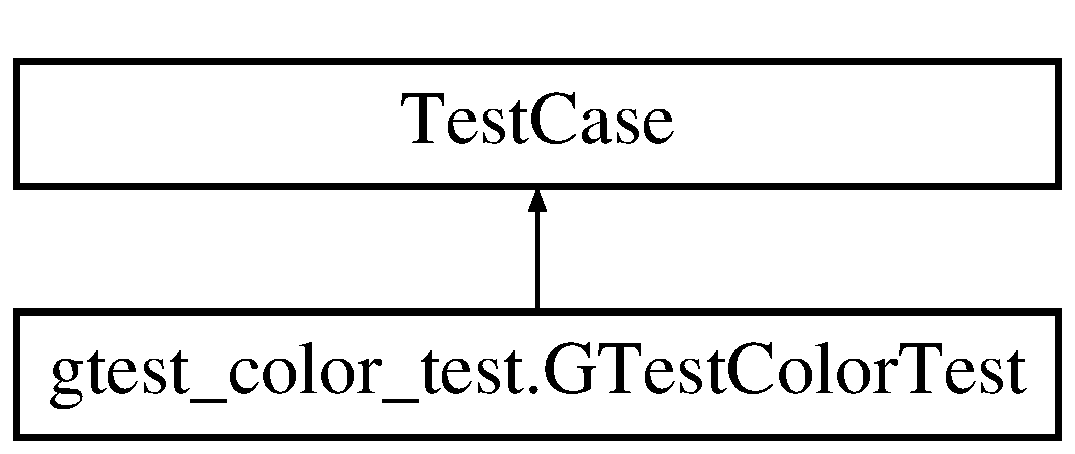
\includegraphics[height=2.000000cm]{classgtest__color__test_1_1_g_test_color_test}
\end{center}
\end{figure}
\subsection*{Public Member Functions}
\begin{DoxyCompactItemize}
\item 
def \mbox{\hyperlink{classgtest__color__test_1_1_g_test_color_test_a22bf83ab416dc3ccd3c1b771ff74022c}{test\+No\+Env\+Var\+No\+Flag}} (self)
\item 
def \mbox{\hyperlink{classgtest__color__test_1_1_g_test_color_test_abc4c056b8e703e83516f9e5aea8dd25d}{test\+Flag\+Only}} (self)
\item 
def \mbox{\hyperlink{classgtest__color__test_1_1_g_test_color_test_aedb7bbaa0d6acff3628d91a471f4ceb5}{test\+Env\+Var\+Only}} (self)
\item 
def \mbox{\hyperlink{classgtest__color__test_1_1_g_test_color_test_ae88e8ec526135ed1448e83fc4ec7cd15}{test\+Env\+Var\+And\+Flag}} (self)
\item 
def \mbox{\hyperlink{classgtest__color__test_1_1_g_test_color_test_aaf2110e359494dc711e87d29d351dc47}{test\+Aliases\+Of\+Yes\+And\+No}} (self)
\end{DoxyCompactItemize}


\subsection{Member Function Documentation}
\mbox{\Hypertarget{classgtest__color__test_1_1_g_test_color_test_aaf2110e359494dc711e87d29d351dc47}\label{classgtest__color__test_1_1_g_test_color_test_aaf2110e359494dc711e87d29d351dc47}} 
\index{gtest\+\_\+color\+\_\+test\+::\+G\+Test\+Color\+Test@{gtest\+\_\+color\+\_\+test\+::\+G\+Test\+Color\+Test}!test\+Aliases\+Of\+Yes\+And\+No@{test\+Aliases\+Of\+Yes\+And\+No}}
\index{test\+Aliases\+Of\+Yes\+And\+No@{test\+Aliases\+Of\+Yes\+And\+No}!gtest\+\_\+color\+\_\+test\+::\+G\+Test\+Color\+Test@{gtest\+\_\+color\+\_\+test\+::\+G\+Test\+Color\+Test}}
\subsubsection{\texorpdfstring{test\+Aliases\+Of\+Yes\+And\+No()}{testAliasesOfYesAndNo()}}
{\footnotesize\ttfamily def gtest\+\_\+color\+\_\+test.\+G\+Test\+Color\+Test.\+test\+Aliases\+Of\+Yes\+And\+No (\begin{DoxyParamCaption}\item[{}]{self }\end{DoxyParamCaption})}

\begin{DoxyVerb}Tests using aliases in specifying --gtest_color.\end{DoxyVerb}
 \mbox{\Hypertarget{classgtest__color__test_1_1_g_test_color_test_ae88e8ec526135ed1448e83fc4ec7cd15}\label{classgtest__color__test_1_1_g_test_color_test_ae88e8ec526135ed1448e83fc4ec7cd15}} 
\index{gtest\+\_\+color\+\_\+test\+::\+G\+Test\+Color\+Test@{gtest\+\_\+color\+\_\+test\+::\+G\+Test\+Color\+Test}!test\+Env\+Var\+And\+Flag@{test\+Env\+Var\+And\+Flag}}
\index{test\+Env\+Var\+And\+Flag@{test\+Env\+Var\+And\+Flag}!gtest\+\_\+color\+\_\+test\+::\+G\+Test\+Color\+Test@{gtest\+\_\+color\+\_\+test\+::\+G\+Test\+Color\+Test}}
\subsubsection{\texorpdfstring{test\+Env\+Var\+And\+Flag()}{testEnvVarAndFlag()}}
{\footnotesize\ttfamily def gtest\+\_\+color\+\_\+test.\+G\+Test\+Color\+Test.\+test\+Env\+Var\+And\+Flag (\begin{DoxyParamCaption}\item[{}]{self }\end{DoxyParamCaption})}

\begin{DoxyVerb}Tests the case when there are both GTEST_COLOR and --gtest_color.\end{DoxyVerb}
 \mbox{\Hypertarget{classgtest__color__test_1_1_g_test_color_test_aedb7bbaa0d6acff3628d91a471f4ceb5}\label{classgtest__color__test_1_1_g_test_color_test_aedb7bbaa0d6acff3628d91a471f4ceb5}} 
\index{gtest\+\_\+color\+\_\+test\+::\+G\+Test\+Color\+Test@{gtest\+\_\+color\+\_\+test\+::\+G\+Test\+Color\+Test}!test\+Env\+Var\+Only@{test\+Env\+Var\+Only}}
\index{test\+Env\+Var\+Only@{test\+Env\+Var\+Only}!gtest\+\_\+color\+\_\+test\+::\+G\+Test\+Color\+Test@{gtest\+\_\+color\+\_\+test\+::\+G\+Test\+Color\+Test}}
\subsubsection{\texorpdfstring{test\+Env\+Var\+Only()}{testEnvVarOnly()}}
{\footnotesize\ttfamily def gtest\+\_\+color\+\_\+test.\+G\+Test\+Color\+Test.\+test\+Env\+Var\+Only (\begin{DoxyParamCaption}\item[{}]{self }\end{DoxyParamCaption})}

\begin{DoxyVerb}Tests the case when there's GTEST_COLOR but not --gtest_color.\end{DoxyVerb}
 \mbox{\Hypertarget{classgtest__color__test_1_1_g_test_color_test_abc4c056b8e703e83516f9e5aea8dd25d}\label{classgtest__color__test_1_1_g_test_color_test_abc4c056b8e703e83516f9e5aea8dd25d}} 
\index{gtest\+\_\+color\+\_\+test\+::\+G\+Test\+Color\+Test@{gtest\+\_\+color\+\_\+test\+::\+G\+Test\+Color\+Test}!test\+Flag\+Only@{test\+Flag\+Only}}
\index{test\+Flag\+Only@{test\+Flag\+Only}!gtest\+\_\+color\+\_\+test\+::\+G\+Test\+Color\+Test@{gtest\+\_\+color\+\_\+test\+::\+G\+Test\+Color\+Test}}
\subsubsection{\texorpdfstring{test\+Flag\+Only()}{testFlagOnly()}}
{\footnotesize\ttfamily def gtest\+\_\+color\+\_\+test.\+G\+Test\+Color\+Test.\+test\+Flag\+Only (\begin{DoxyParamCaption}\item[{}]{self }\end{DoxyParamCaption})}

\begin{DoxyVerb}Tests the case when there's --gtest_color but not GTEST_COLOR.\end{DoxyVerb}
 \mbox{\Hypertarget{classgtest__color__test_1_1_g_test_color_test_a22bf83ab416dc3ccd3c1b771ff74022c}\label{classgtest__color__test_1_1_g_test_color_test_a22bf83ab416dc3ccd3c1b771ff74022c}} 
\index{gtest\+\_\+color\+\_\+test\+::\+G\+Test\+Color\+Test@{gtest\+\_\+color\+\_\+test\+::\+G\+Test\+Color\+Test}!test\+No\+Env\+Var\+No\+Flag@{test\+No\+Env\+Var\+No\+Flag}}
\index{test\+No\+Env\+Var\+No\+Flag@{test\+No\+Env\+Var\+No\+Flag}!gtest\+\_\+color\+\_\+test\+::\+G\+Test\+Color\+Test@{gtest\+\_\+color\+\_\+test\+::\+G\+Test\+Color\+Test}}
\subsubsection{\texorpdfstring{test\+No\+Env\+Var\+No\+Flag()}{testNoEnvVarNoFlag()}}
{\footnotesize\ttfamily def gtest\+\_\+color\+\_\+test.\+G\+Test\+Color\+Test.\+test\+No\+Env\+Var\+No\+Flag (\begin{DoxyParamCaption}\item[{}]{self }\end{DoxyParamCaption})}

\begin{DoxyVerb}Tests the case when there's neither GTEST_COLOR nor --gtest_color.\end{DoxyVerb}
 

The documentation for this class was generated from the following file\+:\begin{DoxyCompactItemize}
\item 
/\+Users/fjp/git/bachelor/bachelor-\/master\+\_\+updated\+\_\+vfinal/googletest-\/1.\+8.\+0/googletest/test/gtest\+\_\+color\+\_\+test.\+py\end{DoxyCompactItemize}

\hypertarget{classgtest__env__var__test_1_1_g_test_env_var_test}{}\section{gtest\+\_\+env\+\_\+var\+\_\+test.\+G\+Test\+Env\+Var\+Test Class Reference}
\label{classgtest__env__var__test_1_1_g_test_env_var_test}\index{gtest\+\_\+env\+\_\+var\+\_\+test.\+G\+Test\+Env\+Var\+Test@{gtest\+\_\+env\+\_\+var\+\_\+test.\+G\+Test\+Env\+Var\+Test}}
Inheritance diagram for gtest\+\_\+env\+\_\+var\+\_\+test.\+G\+Test\+Env\+Var\+Test\+:\begin{figure}[H]
\begin{center}
\leavevmode
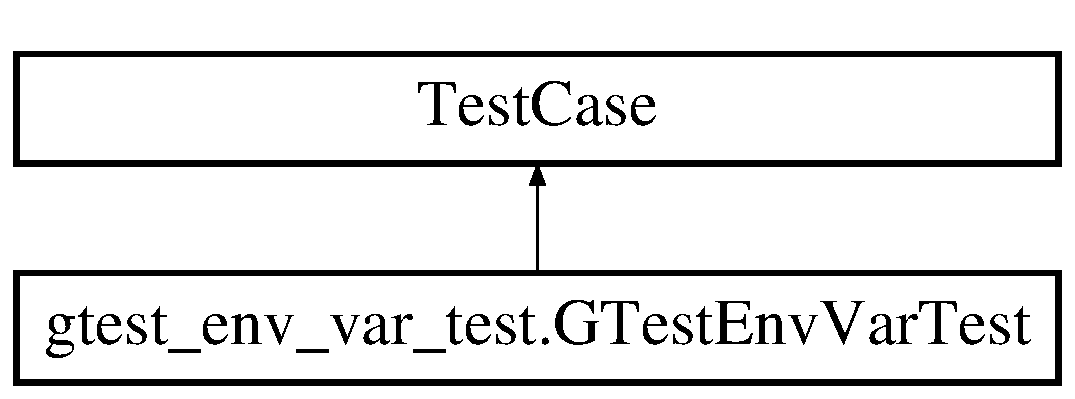
\includegraphics[height=2.000000cm]{classgtest__env__var__test_1_1_g_test_env_var_test}
\end{center}
\end{figure}
\subsection*{Public Member Functions}
\begin{DoxyCompactItemize}
\item 
def \mbox{\hyperlink{classgtest__env__var__test_1_1_g_test_env_var_test_ad169061caa22a6cd510535d6da94b97e}{test\+Env\+Var\+Affects\+Flag}} (self)
\item 
def \mbox{\hyperlink{classgtest__env__var__test_1_1_g_test_env_var_test_ae2f623209c115e094965e606cd34eec4}{test\+Xml\+Output\+File}} (self)
\item 
def \mbox{\hyperlink{classgtest__env__var__test_1_1_g_test_env_var_test_ae41b9b9569eb327d5886cb811c2995a7}{test\+Xml\+Output\+File\+Override}} (self)
\end{DoxyCompactItemize}


\subsection{Member Function Documentation}
\mbox{\Hypertarget{classgtest__env__var__test_1_1_g_test_env_var_test_ad169061caa22a6cd510535d6da94b97e}\label{classgtest__env__var__test_1_1_g_test_env_var_test_ad169061caa22a6cd510535d6da94b97e}} 
\index{gtest\+\_\+env\+\_\+var\+\_\+test\+::\+G\+Test\+Env\+Var\+Test@{gtest\+\_\+env\+\_\+var\+\_\+test\+::\+G\+Test\+Env\+Var\+Test}!test\+Env\+Var\+Affects\+Flag@{test\+Env\+Var\+Affects\+Flag}}
\index{test\+Env\+Var\+Affects\+Flag@{test\+Env\+Var\+Affects\+Flag}!gtest\+\_\+env\+\_\+var\+\_\+test\+::\+G\+Test\+Env\+Var\+Test@{gtest\+\_\+env\+\_\+var\+\_\+test\+::\+G\+Test\+Env\+Var\+Test}}
\subsubsection{\texorpdfstring{test\+Env\+Var\+Affects\+Flag()}{testEnvVarAffectsFlag()}}
{\footnotesize\ttfamily def gtest\+\_\+env\+\_\+var\+\_\+test.\+G\+Test\+Env\+Var\+Test.\+test\+Env\+Var\+Affects\+Flag (\begin{DoxyParamCaption}\item[{}]{self }\end{DoxyParamCaption})}

\begin{DoxyVerb}Tests that environment variable should affect the corresponding flag.\end{DoxyVerb}
 \mbox{\Hypertarget{classgtest__env__var__test_1_1_g_test_env_var_test_ae2f623209c115e094965e606cd34eec4}\label{classgtest__env__var__test_1_1_g_test_env_var_test_ae2f623209c115e094965e606cd34eec4}} 
\index{gtest\+\_\+env\+\_\+var\+\_\+test\+::\+G\+Test\+Env\+Var\+Test@{gtest\+\_\+env\+\_\+var\+\_\+test\+::\+G\+Test\+Env\+Var\+Test}!test\+Xml\+Output\+File@{test\+Xml\+Output\+File}}
\index{test\+Xml\+Output\+File@{test\+Xml\+Output\+File}!gtest\+\_\+env\+\_\+var\+\_\+test\+::\+G\+Test\+Env\+Var\+Test@{gtest\+\_\+env\+\_\+var\+\_\+test\+::\+G\+Test\+Env\+Var\+Test}}
\subsubsection{\texorpdfstring{test\+Xml\+Output\+File()}{testXmlOutputFile()}}
{\footnotesize\ttfamily def gtest\+\_\+env\+\_\+var\+\_\+test.\+G\+Test\+Env\+Var\+Test.\+test\+Xml\+Output\+File (\begin{DoxyParamCaption}\item[{}]{self }\end{DoxyParamCaption})}

\begin{DoxyVerb}Tests that $XML_OUTPUT_FILE affects the output flag.\end{DoxyVerb}
 \mbox{\Hypertarget{classgtest__env__var__test_1_1_g_test_env_var_test_ae41b9b9569eb327d5886cb811c2995a7}\label{classgtest__env__var__test_1_1_g_test_env_var_test_ae41b9b9569eb327d5886cb811c2995a7}} 
\index{gtest\+\_\+env\+\_\+var\+\_\+test\+::\+G\+Test\+Env\+Var\+Test@{gtest\+\_\+env\+\_\+var\+\_\+test\+::\+G\+Test\+Env\+Var\+Test}!test\+Xml\+Output\+File\+Override@{test\+Xml\+Output\+File\+Override}}
\index{test\+Xml\+Output\+File\+Override@{test\+Xml\+Output\+File\+Override}!gtest\+\_\+env\+\_\+var\+\_\+test\+::\+G\+Test\+Env\+Var\+Test@{gtest\+\_\+env\+\_\+var\+\_\+test\+::\+G\+Test\+Env\+Var\+Test}}
\subsubsection{\texorpdfstring{test\+Xml\+Output\+File\+Override()}{testXmlOutputFileOverride()}}
{\footnotesize\ttfamily def gtest\+\_\+env\+\_\+var\+\_\+test.\+G\+Test\+Env\+Var\+Test.\+test\+Xml\+Output\+File\+Override (\begin{DoxyParamCaption}\item[{}]{self }\end{DoxyParamCaption})}

\begin{DoxyVerb}Tests that $XML_OUTPUT_FILE is overridden by $GTEST_OUTPUT\end{DoxyVerb}
 

The documentation for this class was generated from the following file\+:\begin{DoxyCompactItemize}
\item 
/\+Users/fjp/git/bachelor/bachelor-\/master\+\_\+updated\+\_\+vfinal/googletest-\/1.\+8.\+0/googletest/test/gtest\+\_\+env\+\_\+var\+\_\+test.\+py\end{DoxyCompactItemize}

\hypertarget{classgtest__filter__unittest_1_1_g_test_filter_unit_test}{}\section{gtest\+\_\+filter\+\_\+unittest.\+G\+Test\+Filter\+Unit\+Test Class Reference}
\label{classgtest__filter__unittest_1_1_g_test_filter_unit_test}\index{gtest\+\_\+filter\+\_\+unittest.\+G\+Test\+Filter\+Unit\+Test@{gtest\+\_\+filter\+\_\+unittest.\+G\+Test\+Filter\+Unit\+Test}}
Inheritance diagram for gtest\+\_\+filter\+\_\+unittest.\+G\+Test\+Filter\+Unit\+Test\+:\begin{figure}[H]
\begin{center}
\leavevmode
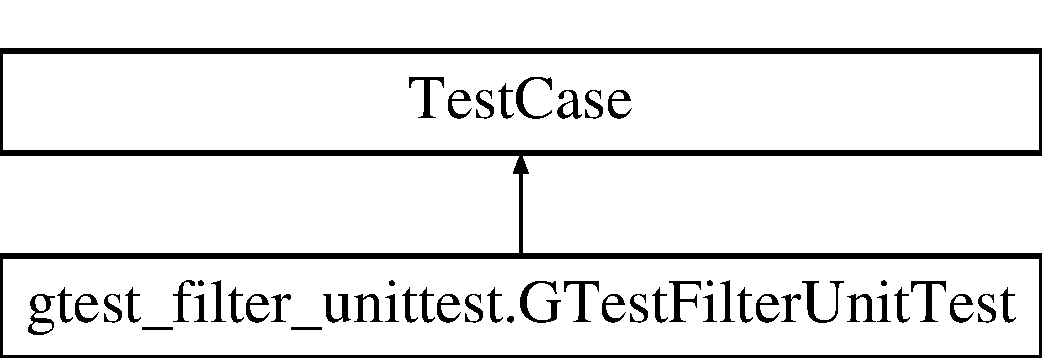
\includegraphics[height=2.000000cm]{classgtest__filter__unittest_1_1_g_test_filter_unit_test}
\end{center}
\end{figure}
\subsection*{Public Member Functions}
\begin{DoxyCompactItemize}
\item 
def \mbox{\hyperlink{classgtest__filter__unittest_1_1_g_test_filter_unit_test_aeebdbdcc59594ad0a69cf11eafe94997}{Assert\+Set\+Equal}} (self, lhs, rhs)
\item 
def \mbox{\hyperlink{classgtest__filter__unittest_1_1_g_test_filter_unit_test_a87656eac0cf4136252eef43da0121381}{Assert\+Partition\+Is\+Valid}} (self, set\+\_\+var, list\+\_\+of\+\_\+sets)
\item 
def \mbox{\hyperlink{classgtest__filter__unittest_1_1_g_test_filter_unit_test_a11c48bf404bca6806b14a1a71d169ace}{Adjust\+For\+Parameterized\+Tests}} (self, tests\+\_\+to\+\_\+run)
\item 
def \mbox{\hyperlink{classgtest__filter__unittest_1_1_g_test_filter_unit_test_acf341ed9a265b346a050afa9a9a85c65}{Run\+And\+Verify}} (self, gtest\+\_\+filter, tests\+\_\+to\+\_\+run)
\item 
def \mbox{\hyperlink{classgtest__filter__unittest_1_1_g_test_filter_unit_test_a2022ed99e18a6e5afd1023b9dd19d6e0}{Run\+And\+Verify\+With\+Sharding}} (self, gtest\+\_\+filter, total\+\_\+shards, tests\+\_\+to\+\_\+run, args=None, check\+\_\+exit\+\_\+0=False)
\item 
def \mbox{\hyperlink{classgtest__filter__unittest_1_1_g_test_filter_unit_test_ae52bd70ef1dcb68c83c0379ddfb987a9}{Run\+And\+Verify\+Allowing\+Disabled}} (self, gtest\+\_\+filter, tests\+\_\+to\+\_\+run)
\item 
def \mbox{\hyperlink{classgtest__filter__unittest_1_1_g_test_filter_unit_test_af20a71b1659314a5cc1093d77a673495}{set\+Up}} (self)
\item 
def \mbox{\hyperlink{classgtest__filter__unittest_1_1_g_test_filter_unit_test_adef3a9b539c73bda785a631a5aac424f}{test\+Default\+Behavior}} (self)
\item 
def \mbox{\hyperlink{classgtest__filter__unittest_1_1_g_test_filter_unit_test_a8d5ad564f41c052864a3957a71daa535}{test\+Default\+Behavior\+With\+Shards}} (self)
\item 
def \mbox{\hyperlink{classgtest__filter__unittest_1_1_g_test_filter_unit_test_afce65847b463ec5bca4458e9348d9a9f}{test\+Empty\+Filter}} (self)
\item 
def \mbox{\hyperlink{classgtest__filter__unittest_1_1_g_test_filter_unit_test_a2456062c177350a53244aea030aaf617}{test\+Bad\+Filter}} (self)
\item 
def \mbox{\hyperlink{classgtest__filter__unittest_1_1_g_test_filter_unit_test_a336d9203e26493bae11fbb514af38a6b}{test\+Full\+Name}} (self)
\item 
def \mbox{\hyperlink{classgtest__filter__unittest_1_1_g_test_filter_unit_test_ae9da48a79483e22e3f986e57de0dee37}{test\+Universal\+Filters}} (self)
\item 
def \mbox{\hyperlink{classgtest__filter__unittest_1_1_g_test_filter_unit_test_ac59206c94324afdc09adbe5853856174}{test\+Filter\+By\+Test\+Case}} (self)
\item 
def \mbox{\hyperlink{classgtest__filter__unittest_1_1_g_test_filter_unit_test_aaea691324a6c0765403b26a895702a63}{test\+Filter\+By\+Test}} (self)
\item 
def \mbox{\hyperlink{classgtest__filter__unittest_1_1_g_test_filter_unit_test_a6d962adae2ee2697b3b92e84b60a795a}{test\+Filter\+Disabled\+Tests}} (self)
\item 
def \mbox{\hyperlink{classgtest__filter__unittest_1_1_g_test_filter_unit_test_af855132606c1fa02fb765e8619108114}{test\+Wildcard\+In\+Test\+Case\+Name}} (self)
\item 
def \mbox{\hyperlink{classgtest__filter__unittest_1_1_g_test_filter_unit_test_a9b1e6b35e158d7c6d11b8f4d2cb600cb}{test\+Wildcard\+In\+Test\+Name}} (self)
\item 
def \mbox{\hyperlink{classgtest__filter__unittest_1_1_g_test_filter_unit_test_a874aea28690300d8c0dc0910304f7ab2}{test\+Filter\+Without\+Dot}} (self)
\item 
def \mbox{\hyperlink{classgtest__filter__unittest_1_1_g_test_filter_unit_test_a2563885e647205586b135c5ead55e6ab}{test\+Two\+Patterns}} (self)
\item 
def \mbox{\hyperlink{classgtest__filter__unittest_1_1_g_test_filter_unit_test_af4858e153245f0974632fd36dc1dd804}{test\+Three\+Patterns}} (self)
\item 
\mbox{\Hypertarget{classgtest__filter__unittest_1_1_g_test_filter_unit_test_aff878809d524797f62e2fe38bbfcc8da}\label{classgtest__filter__unittest_1_1_g_test_filter_unit_test_aff878809d524797f62e2fe38bbfcc8da}} 
def {\bfseries test\+Negative\+Filters} (self)
\item 
def \mbox{\hyperlink{classgtest__filter__unittest_1_1_g_test_filter_unit_test_a81e4256da0e0ad8cb4b764ffd573cc6d}{test\+Flag\+Overrides\+Env\+Var}} (self)
\item 
def \mbox{\hyperlink{classgtest__filter__unittest_1_1_g_test_filter_unit_test_a7a2c7b8d758abba0ae883bbb272f344b}{test\+Shard\+Status\+File\+Is\+Created}} (self)
\item 
def \mbox{\hyperlink{classgtest__filter__unittest_1_1_g_test_filter_unit_test_a1dac68948f6170e39ae9ee7bca0bc1eb}{test\+Shard\+Status\+File\+Is\+Created\+With\+List\+Tests}} (self)
\item 
def \mbox{\hyperlink{classgtest__filter__unittest_1_1_g_test_filter_unit_test_a4b4f7428d9219dff5960968477927626}{test\+Sharding\+Works\+With\+Death\+Tests}} (self)
\end{DoxyCompactItemize}


\subsection{Detailed Description}
\begin{DoxyVerb}Tests the env variable or the command line flag to filter tests.\end{DoxyVerb}
 

\subsection{Member Function Documentation}
\mbox{\Hypertarget{classgtest__filter__unittest_1_1_g_test_filter_unit_test_a11c48bf404bca6806b14a1a71d169ace}\label{classgtest__filter__unittest_1_1_g_test_filter_unit_test_a11c48bf404bca6806b14a1a71d169ace}} 
\index{gtest\+\_\+filter\+\_\+unittest\+::\+G\+Test\+Filter\+Unit\+Test@{gtest\+\_\+filter\+\_\+unittest\+::\+G\+Test\+Filter\+Unit\+Test}!Adjust\+For\+Parameterized\+Tests@{Adjust\+For\+Parameterized\+Tests}}
\index{Adjust\+For\+Parameterized\+Tests@{Adjust\+For\+Parameterized\+Tests}!gtest\+\_\+filter\+\_\+unittest\+::\+G\+Test\+Filter\+Unit\+Test@{gtest\+\_\+filter\+\_\+unittest\+::\+G\+Test\+Filter\+Unit\+Test}}
\subsubsection{\texorpdfstring{Adjust\+For\+Parameterized\+Tests()}{AdjustForParameterizedTests()}}
{\footnotesize\ttfamily def gtest\+\_\+filter\+\_\+unittest.\+G\+Test\+Filter\+Unit\+Test.\+Adjust\+For\+Parameterized\+Tests (\begin{DoxyParamCaption}\item[{}]{self,  }\item[{}]{tests\+\_\+to\+\_\+run }\end{DoxyParamCaption})}

\begin{DoxyVerb}Adjust tests_to_run in case value parameterized tests are disabled.\end{DoxyVerb}
 \mbox{\Hypertarget{classgtest__filter__unittest_1_1_g_test_filter_unit_test_a87656eac0cf4136252eef43da0121381}\label{classgtest__filter__unittest_1_1_g_test_filter_unit_test_a87656eac0cf4136252eef43da0121381}} 
\index{gtest\+\_\+filter\+\_\+unittest\+::\+G\+Test\+Filter\+Unit\+Test@{gtest\+\_\+filter\+\_\+unittest\+::\+G\+Test\+Filter\+Unit\+Test}!Assert\+Partition\+Is\+Valid@{Assert\+Partition\+Is\+Valid}}
\index{Assert\+Partition\+Is\+Valid@{Assert\+Partition\+Is\+Valid}!gtest\+\_\+filter\+\_\+unittest\+::\+G\+Test\+Filter\+Unit\+Test@{gtest\+\_\+filter\+\_\+unittest\+::\+G\+Test\+Filter\+Unit\+Test}}
\subsubsection{\texorpdfstring{Assert\+Partition\+Is\+Valid()}{AssertPartitionIsValid()}}
{\footnotesize\ttfamily def gtest\+\_\+filter\+\_\+unittest.\+G\+Test\+Filter\+Unit\+Test.\+Assert\+Partition\+Is\+Valid (\begin{DoxyParamCaption}\item[{}]{self,  }\item[{}]{set\+\_\+var,  }\item[{}]{list\+\_\+of\+\_\+sets }\end{DoxyParamCaption})}

\begin{DoxyVerb}Asserts that list_of_sets is a valid partition of set_var.\end{DoxyVerb}
 \mbox{\Hypertarget{classgtest__filter__unittest_1_1_g_test_filter_unit_test_aeebdbdcc59594ad0a69cf11eafe94997}\label{classgtest__filter__unittest_1_1_g_test_filter_unit_test_aeebdbdcc59594ad0a69cf11eafe94997}} 
\index{gtest\+\_\+filter\+\_\+unittest\+::\+G\+Test\+Filter\+Unit\+Test@{gtest\+\_\+filter\+\_\+unittest\+::\+G\+Test\+Filter\+Unit\+Test}!Assert\+Set\+Equal@{Assert\+Set\+Equal}}
\index{Assert\+Set\+Equal@{Assert\+Set\+Equal}!gtest\+\_\+filter\+\_\+unittest\+::\+G\+Test\+Filter\+Unit\+Test@{gtest\+\_\+filter\+\_\+unittest\+::\+G\+Test\+Filter\+Unit\+Test}}
\subsubsection{\texorpdfstring{Assert\+Set\+Equal()}{AssertSetEqual()}}
{\footnotesize\ttfamily def gtest\+\_\+filter\+\_\+unittest.\+G\+Test\+Filter\+Unit\+Test.\+Assert\+Set\+Equal (\begin{DoxyParamCaption}\item[{}]{self,  }\item[{}]{lhs,  }\item[{}]{rhs }\end{DoxyParamCaption})}

\begin{DoxyVerb}Asserts that two sets are equal.\end{DoxyVerb}
 \mbox{\Hypertarget{classgtest__filter__unittest_1_1_g_test_filter_unit_test_acf341ed9a265b346a050afa9a9a85c65}\label{classgtest__filter__unittest_1_1_g_test_filter_unit_test_acf341ed9a265b346a050afa9a9a85c65}} 
\index{gtest\+\_\+filter\+\_\+unittest\+::\+G\+Test\+Filter\+Unit\+Test@{gtest\+\_\+filter\+\_\+unittest\+::\+G\+Test\+Filter\+Unit\+Test}!Run\+And\+Verify@{Run\+And\+Verify}}
\index{Run\+And\+Verify@{Run\+And\+Verify}!gtest\+\_\+filter\+\_\+unittest\+::\+G\+Test\+Filter\+Unit\+Test@{gtest\+\_\+filter\+\_\+unittest\+::\+G\+Test\+Filter\+Unit\+Test}}
\subsubsection{\texorpdfstring{Run\+And\+Verify()}{RunAndVerify()}}
{\footnotesize\ttfamily def gtest\+\_\+filter\+\_\+unittest.\+G\+Test\+Filter\+Unit\+Test.\+Run\+And\+Verify (\begin{DoxyParamCaption}\item[{}]{self,  }\item[{}]{gtest\+\_\+filter,  }\item[{}]{tests\+\_\+to\+\_\+run }\end{DoxyParamCaption})}

\begin{DoxyVerb}Checks that the binary runs correct set of tests for a given filter.\end{DoxyVerb}
 \mbox{\Hypertarget{classgtest__filter__unittest_1_1_g_test_filter_unit_test_ae52bd70ef1dcb68c83c0379ddfb987a9}\label{classgtest__filter__unittest_1_1_g_test_filter_unit_test_ae52bd70ef1dcb68c83c0379ddfb987a9}} 
\index{gtest\+\_\+filter\+\_\+unittest\+::\+G\+Test\+Filter\+Unit\+Test@{gtest\+\_\+filter\+\_\+unittest\+::\+G\+Test\+Filter\+Unit\+Test}!Run\+And\+Verify\+Allowing\+Disabled@{Run\+And\+Verify\+Allowing\+Disabled}}
\index{Run\+And\+Verify\+Allowing\+Disabled@{Run\+And\+Verify\+Allowing\+Disabled}!gtest\+\_\+filter\+\_\+unittest\+::\+G\+Test\+Filter\+Unit\+Test@{gtest\+\_\+filter\+\_\+unittest\+::\+G\+Test\+Filter\+Unit\+Test}}
\subsubsection{\texorpdfstring{Run\+And\+Verify\+Allowing\+Disabled()}{RunAndVerifyAllowingDisabled()}}
{\footnotesize\ttfamily def gtest\+\_\+filter\+\_\+unittest.\+G\+Test\+Filter\+Unit\+Test.\+Run\+And\+Verify\+Allowing\+Disabled (\begin{DoxyParamCaption}\item[{}]{self,  }\item[{}]{gtest\+\_\+filter,  }\item[{}]{tests\+\_\+to\+\_\+run }\end{DoxyParamCaption})}

\begin{DoxyVerb}Checks that the binary runs correct set of tests for the given filter.

Runs gtest_filter_unittest_ with the given filter, and enables
disabled tests. Verifies that the right set of tests were run.

Args:
  gtest_filter: A filter to apply to the tests.
  tests_to_run: A set of tests expected to run.
\end{DoxyVerb}
 \mbox{\Hypertarget{classgtest__filter__unittest_1_1_g_test_filter_unit_test_a2022ed99e18a6e5afd1023b9dd19d6e0}\label{classgtest__filter__unittest_1_1_g_test_filter_unit_test_a2022ed99e18a6e5afd1023b9dd19d6e0}} 
\index{gtest\+\_\+filter\+\_\+unittest\+::\+G\+Test\+Filter\+Unit\+Test@{gtest\+\_\+filter\+\_\+unittest\+::\+G\+Test\+Filter\+Unit\+Test}!Run\+And\+Verify\+With\+Sharding@{Run\+And\+Verify\+With\+Sharding}}
\index{Run\+And\+Verify\+With\+Sharding@{Run\+And\+Verify\+With\+Sharding}!gtest\+\_\+filter\+\_\+unittest\+::\+G\+Test\+Filter\+Unit\+Test@{gtest\+\_\+filter\+\_\+unittest\+::\+G\+Test\+Filter\+Unit\+Test}}
\subsubsection{\texorpdfstring{Run\+And\+Verify\+With\+Sharding()}{RunAndVerifyWithSharding()}}
{\footnotesize\ttfamily def gtest\+\_\+filter\+\_\+unittest.\+G\+Test\+Filter\+Unit\+Test.\+Run\+And\+Verify\+With\+Sharding (\begin{DoxyParamCaption}\item[{}]{self,  }\item[{}]{gtest\+\_\+filter,  }\item[{}]{total\+\_\+shards,  }\item[{}]{tests\+\_\+to\+\_\+run,  }\item[{}]{args = {\ttfamily None},  }\item[{}]{check\+\_\+exit\+\_\+0 = {\ttfamily False} }\end{DoxyParamCaption})}

\begin{DoxyVerb}Checks that binary runs correct tests for the given filter and shard.

Runs all shards of gtest_filter_unittest_ with the given filter, and
verifies that the right set of tests were run. The union of tests run
on each shard should be identical to tests_to_run, without duplicates.

Args:
  gtest_filter: A filter to apply to the tests.
  total_shards: A total number of shards to split test run into.
  tests_to_run: A set of tests expected to run.
  args   :      Arguments to pass to the to the test binary.
  check_exit_0: When set to a true value, make sure that all shards
            return 0.
\end{DoxyVerb}
 \mbox{\Hypertarget{classgtest__filter__unittest_1_1_g_test_filter_unit_test_af20a71b1659314a5cc1093d77a673495}\label{classgtest__filter__unittest_1_1_g_test_filter_unit_test_af20a71b1659314a5cc1093d77a673495}} 
\index{gtest\+\_\+filter\+\_\+unittest\+::\+G\+Test\+Filter\+Unit\+Test@{gtest\+\_\+filter\+\_\+unittest\+::\+G\+Test\+Filter\+Unit\+Test}!set\+Up@{set\+Up}}
\index{set\+Up@{set\+Up}!gtest\+\_\+filter\+\_\+unittest\+::\+G\+Test\+Filter\+Unit\+Test@{gtest\+\_\+filter\+\_\+unittest\+::\+G\+Test\+Filter\+Unit\+Test}}
\subsubsection{\texorpdfstring{set\+Up()}{setUp()}}
{\footnotesize\ttfamily def gtest\+\_\+filter\+\_\+unittest.\+G\+Test\+Filter\+Unit\+Test.\+set\+Up (\begin{DoxyParamCaption}\item[{}]{self }\end{DoxyParamCaption})}

\begin{DoxyVerb}Sets up test case.

Determines whether value-parameterized tests are enabled in the binary and
sets the flags accordingly.
\end{DoxyVerb}
 \mbox{\Hypertarget{classgtest__filter__unittest_1_1_g_test_filter_unit_test_a2456062c177350a53244aea030aaf617}\label{classgtest__filter__unittest_1_1_g_test_filter_unit_test_a2456062c177350a53244aea030aaf617}} 
\index{gtest\+\_\+filter\+\_\+unittest\+::\+G\+Test\+Filter\+Unit\+Test@{gtest\+\_\+filter\+\_\+unittest\+::\+G\+Test\+Filter\+Unit\+Test}!test\+Bad\+Filter@{test\+Bad\+Filter}}
\index{test\+Bad\+Filter@{test\+Bad\+Filter}!gtest\+\_\+filter\+\_\+unittest\+::\+G\+Test\+Filter\+Unit\+Test@{gtest\+\_\+filter\+\_\+unittest\+::\+G\+Test\+Filter\+Unit\+Test}}
\subsubsection{\texorpdfstring{test\+Bad\+Filter()}{testBadFilter()}}
{\footnotesize\ttfamily def gtest\+\_\+filter\+\_\+unittest.\+G\+Test\+Filter\+Unit\+Test.\+test\+Bad\+Filter (\begin{DoxyParamCaption}\item[{}]{self }\end{DoxyParamCaption})}

\begin{DoxyVerb}Tests a filter that matches nothing.\end{DoxyVerb}
 \mbox{\Hypertarget{classgtest__filter__unittest_1_1_g_test_filter_unit_test_adef3a9b539c73bda785a631a5aac424f}\label{classgtest__filter__unittest_1_1_g_test_filter_unit_test_adef3a9b539c73bda785a631a5aac424f}} 
\index{gtest\+\_\+filter\+\_\+unittest\+::\+G\+Test\+Filter\+Unit\+Test@{gtest\+\_\+filter\+\_\+unittest\+::\+G\+Test\+Filter\+Unit\+Test}!test\+Default\+Behavior@{test\+Default\+Behavior}}
\index{test\+Default\+Behavior@{test\+Default\+Behavior}!gtest\+\_\+filter\+\_\+unittest\+::\+G\+Test\+Filter\+Unit\+Test@{gtest\+\_\+filter\+\_\+unittest\+::\+G\+Test\+Filter\+Unit\+Test}}
\subsubsection{\texorpdfstring{test\+Default\+Behavior()}{testDefaultBehavior()}}
{\footnotesize\ttfamily def gtest\+\_\+filter\+\_\+unittest.\+G\+Test\+Filter\+Unit\+Test.\+test\+Default\+Behavior (\begin{DoxyParamCaption}\item[{}]{self }\end{DoxyParamCaption})}

\begin{DoxyVerb}Tests the behavior of not specifying the filter.\end{DoxyVerb}
 \mbox{\Hypertarget{classgtest__filter__unittest_1_1_g_test_filter_unit_test_a8d5ad564f41c052864a3957a71daa535}\label{classgtest__filter__unittest_1_1_g_test_filter_unit_test_a8d5ad564f41c052864a3957a71daa535}} 
\index{gtest\+\_\+filter\+\_\+unittest\+::\+G\+Test\+Filter\+Unit\+Test@{gtest\+\_\+filter\+\_\+unittest\+::\+G\+Test\+Filter\+Unit\+Test}!test\+Default\+Behavior\+With\+Shards@{test\+Default\+Behavior\+With\+Shards}}
\index{test\+Default\+Behavior\+With\+Shards@{test\+Default\+Behavior\+With\+Shards}!gtest\+\_\+filter\+\_\+unittest\+::\+G\+Test\+Filter\+Unit\+Test@{gtest\+\_\+filter\+\_\+unittest\+::\+G\+Test\+Filter\+Unit\+Test}}
\subsubsection{\texorpdfstring{test\+Default\+Behavior\+With\+Shards()}{testDefaultBehaviorWithShards()}}
{\footnotesize\ttfamily def gtest\+\_\+filter\+\_\+unittest.\+G\+Test\+Filter\+Unit\+Test.\+test\+Default\+Behavior\+With\+Shards (\begin{DoxyParamCaption}\item[{}]{self }\end{DoxyParamCaption})}

\begin{DoxyVerb}Tests the behavior without the filter, with sharding enabled.\end{DoxyVerb}
 \mbox{\Hypertarget{classgtest__filter__unittest_1_1_g_test_filter_unit_test_afce65847b463ec5bca4458e9348d9a9f}\label{classgtest__filter__unittest_1_1_g_test_filter_unit_test_afce65847b463ec5bca4458e9348d9a9f}} 
\index{gtest\+\_\+filter\+\_\+unittest\+::\+G\+Test\+Filter\+Unit\+Test@{gtest\+\_\+filter\+\_\+unittest\+::\+G\+Test\+Filter\+Unit\+Test}!test\+Empty\+Filter@{test\+Empty\+Filter}}
\index{test\+Empty\+Filter@{test\+Empty\+Filter}!gtest\+\_\+filter\+\_\+unittest\+::\+G\+Test\+Filter\+Unit\+Test@{gtest\+\_\+filter\+\_\+unittest\+::\+G\+Test\+Filter\+Unit\+Test}}
\subsubsection{\texorpdfstring{test\+Empty\+Filter()}{testEmptyFilter()}}
{\footnotesize\ttfamily def gtest\+\_\+filter\+\_\+unittest.\+G\+Test\+Filter\+Unit\+Test.\+test\+Empty\+Filter (\begin{DoxyParamCaption}\item[{}]{self }\end{DoxyParamCaption})}

\begin{DoxyVerb}Tests an empty filter.\end{DoxyVerb}
 \mbox{\Hypertarget{classgtest__filter__unittest_1_1_g_test_filter_unit_test_aaea691324a6c0765403b26a895702a63}\label{classgtest__filter__unittest_1_1_g_test_filter_unit_test_aaea691324a6c0765403b26a895702a63}} 
\index{gtest\+\_\+filter\+\_\+unittest\+::\+G\+Test\+Filter\+Unit\+Test@{gtest\+\_\+filter\+\_\+unittest\+::\+G\+Test\+Filter\+Unit\+Test}!test\+Filter\+By\+Test@{test\+Filter\+By\+Test}}
\index{test\+Filter\+By\+Test@{test\+Filter\+By\+Test}!gtest\+\_\+filter\+\_\+unittest\+::\+G\+Test\+Filter\+Unit\+Test@{gtest\+\_\+filter\+\_\+unittest\+::\+G\+Test\+Filter\+Unit\+Test}}
\subsubsection{\texorpdfstring{test\+Filter\+By\+Test()}{testFilterByTest()}}
{\footnotesize\ttfamily def gtest\+\_\+filter\+\_\+unittest.\+G\+Test\+Filter\+Unit\+Test.\+test\+Filter\+By\+Test (\begin{DoxyParamCaption}\item[{}]{self }\end{DoxyParamCaption})}

\begin{DoxyVerb}Tests filtering by test name.\end{DoxyVerb}
 \mbox{\Hypertarget{classgtest__filter__unittest_1_1_g_test_filter_unit_test_ac59206c94324afdc09adbe5853856174}\label{classgtest__filter__unittest_1_1_g_test_filter_unit_test_ac59206c94324afdc09adbe5853856174}} 
\index{gtest\+\_\+filter\+\_\+unittest\+::\+G\+Test\+Filter\+Unit\+Test@{gtest\+\_\+filter\+\_\+unittest\+::\+G\+Test\+Filter\+Unit\+Test}!test\+Filter\+By\+Test\+Case@{test\+Filter\+By\+Test\+Case}}
\index{test\+Filter\+By\+Test\+Case@{test\+Filter\+By\+Test\+Case}!gtest\+\_\+filter\+\_\+unittest\+::\+G\+Test\+Filter\+Unit\+Test@{gtest\+\_\+filter\+\_\+unittest\+::\+G\+Test\+Filter\+Unit\+Test}}
\subsubsection{\texorpdfstring{test\+Filter\+By\+Test\+Case()}{testFilterByTestCase()}}
{\footnotesize\ttfamily def gtest\+\_\+filter\+\_\+unittest.\+G\+Test\+Filter\+Unit\+Test.\+test\+Filter\+By\+Test\+Case (\begin{DoxyParamCaption}\item[{}]{self }\end{DoxyParamCaption})}

\begin{DoxyVerb}Tests filtering by test case name.\end{DoxyVerb}
 \mbox{\Hypertarget{classgtest__filter__unittest_1_1_g_test_filter_unit_test_a6d962adae2ee2697b3b92e84b60a795a}\label{classgtest__filter__unittest_1_1_g_test_filter_unit_test_a6d962adae2ee2697b3b92e84b60a795a}} 
\index{gtest\+\_\+filter\+\_\+unittest\+::\+G\+Test\+Filter\+Unit\+Test@{gtest\+\_\+filter\+\_\+unittest\+::\+G\+Test\+Filter\+Unit\+Test}!test\+Filter\+Disabled\+Tests@{test\+Filter\+Disabled\+Tests}}
\index{test\+Filter\+Disabled\+Tests@{test\+Filter\+Disabled\+Tests}!gtest\+\_\+filter\+\_\+unittest\+::\+G\+Test\+Filter\+Unit\+Test@{gtest\+\_\+filter\+\_\+unittest\+::\+G\+Test\+Filter\+Unit\+Test}}
\subsubsection{\texorpdfstring{test\+Filter\+Disabled\+Tests()}{testFilterDisabledTests()}}
{\footnotesize\ttfamily def gtest\+\_\+filter\+\_\+unittest.\+G\+Test\+Filter\+Unit\+Test.\+test\+Filter\+Disabled\+Tests (\begin{DoxyParamCaption}\item[{}]{self }\end{DoxyParamCaption})}

\begin{DoxyVerb}Select only the disabled tests to run.\end{DoxyVerb}
 \mbox{\Hypertarget{classgtest__filter__unittest_1_1_g_test_filter_unit_test_a874aea28690300d8c0dc0910304f7ab2}\label{classgtest__filter__unittest_1_1_g_test_filter_unit_test_a874aea28690300d8c0dc0910304f7ab2}} 
\index{gtest\+\_\+filter\+\_\+unittest\+::\+G\+Test\+Filter\+Unit\+Test@{gtest\+\_\+filter\+\_\+unittest\+::\+G\+Test\+Filter\+Unit\+Test}!test\+Filter\+Without\+Dot@{test\+Filter\+Without\+Dot}}
\index{test\+Filter\+Without\+Dot@{test\+Filter\+Without\+Dot}!gtest\+\_\+filter\+\_\+unittest\+::\+G\+Test\+Filter\+Unit\+Test@{gtest\+\_\+filter\+\_\+unittest\+::\+G\+Test\+Filter\+Unit\+Test}}
\subsubsection{\texorpdfstring{test\+Filter\+Without\+Dot()}{testFilterWithoutDot()}}
{\footnotesize\ttfamily def gtest\+\_\+filter\+\_\+unittest.\+G\+Test\+Filter\+Unit\+Test.\+test\+Filter\+Without\+Dot (\begin{DoxyParamCaption}\item[{}]{self }\end{DoxyParamCaption})}

\begin{DoxyVerb}Tests a filter that has no '.' in it.\end{DoxyVerb}
 \mbox{\Hypertarget{classgtest__filter__unittest_1_1_g_test_filter_unit_test_a81e4256da0e0ad8cb4b764ffd573cc6d}\label{classgtest__filter__unittest_1_1_g_test_filter_unit_test_a81e4256da0e0ad8cb4b764ffd573cc6d}} 
\index{gtest\+\_\+filter\+\_\+unittest\+::\+G\+Test\+Filter\+Unit\+Test@{gtest\+\_\+filter\+\_\+unittest\+::\+G\+Test\+Filter\+Unit\+Test}!test\+Flag\+Overrides\+Env\+Var@{test\+Flag\+Overrides\+Env\+Var}}
\index{test\+Flag\+Overrides\+Env\+Var@{test\+Flag\+Overrides\+Env\+Var}!gtest\+\_\+filter\+\_\+unittest\+::\+G\+Test\+Filter\+Unit\+Test@{gtest\+\_\+filter\+\_\+unittest\+::\+G\+Test\+Filter\+Unit\+Test}}
\subsubsection{\texorpdfstring{test\+Flag\+Overrides\+Env\+Var()}{testFlagOverridesEnvVar()}}
{\footnotesize\ttfamily def gtest\+\_\+filter\+\_\+unittest.\+G\+Test\+Filter\+Unit\+Test.\+test\+Flag\+Overrides\+Env\+Var (\begin{DoxyParamCaption}\item[{}]{self }\end{DoxyParamCaption})}

\begin{DoxyVerb}Tests that the filter flag overrides the filtering env. variable.\end{DoxyVerb}
 \mbox{\Hypertarget{classgtest__filter__unittest_1_1_g_test_filter_unit_test_a336d9203e26493bae11fbb514af38a6b}\label{classgtest__filter__unittest_1_1_g_test_filter_unit_test_a336d9203e26493bae11fbb514af38a6b}} 
\index{gtest\+\_\+filter\+\_\+unittest\+::\+G\+Test\+Filter\+Unit\+Test@{gtest\+\_\+filter\+\_\+unittest\+::\+G\+Test\+Filter\+Unit\+Test}!test\+Full\+Name@{test\+Full\+Name}}
\index{test\+Full\+Name@{test\+Full\+Name}!gtest\+\_\+filter\+\_\+unittest\+::\+G\+Test\+Filter\+Unit\+Test@{gtest\+\_\+filter\+\_\+unittest\+::\+G\+Test\+Filter\+Unit\+Test}}
\subsubsection{\texorpdfstring{test\+Full\+Name()}{testFullName()}}
{\footnotesize\ttfamily def gtest\+\_\+filter\+\_\+unittest.\+G\+Test\+Filter\+Unit\+Test.\+test\+Full\+Name (\begin{DoxyParamCaption}\item[{}]{self }\end{DoxyParamCaption})}

\begin{DoxyVerb}Tests filtering by full name.\end{DoxyVerb}
 \mbox{\Hypertarget{classgtest__filter__unittest_1_1_g_test_filter_unit_test_a4b4f7428d9219dff5960968477927626}\label{classgtest__filter__unittest_1_1_g_test_filter_unit_test_a4b4f7428d9219dff5960968477927626}} 
\index{gtest\+\_\+filter\+\_\+unittest\+::\+G\+Test\+Filter\+Unit\+Test@{gtest\+\_\+filter\+\_\+unittest\+::\+G\+Test\+Filter\+Unit\+Test}!test\+Sharding\+Works\+With\+Death\+Tests@{test\+Sharding\+Works\+With\+Death\+Tests}}
\index{test\+Sharding\+Works\+With\+Death\+Tests@{test\+Sharding\+Works\+With\+Death\+Tests}!gtest\+\_\+filter\+\_\+unittest\+::\+G\+Test\+Filter\+Unit\+Test@{gtest\+\_\+filter\+\_\+unittest\+::\+G\+Test\+Filter\+Unit\+Test}}
\subsubsection{\texorpdfstring{test\+Sharding\+Works\+With\+Death\+Tests()}{testShardingWorksWithDeathTests()}}
{\footnotesize\ttfamily def gtest\+\_\+filter\+\_\+unittest.\+G\+Test\+Filter\+Unit\+Test.\+test\+Sharding\+Works\+With\+Death\+Tests (\begin{DoxyParamCaption}\item[{}]{self }\end{DoxyParamCaption})}

\begin{DoxyVerb}Tests integration with death tests and sharding.\end{DoxyVerb}
 \mbox{\Hypertarget{classgtest__filter__unittest_1_1_g_test_filter_unit_test_a7a2c7b8d758abba0ae883bbb272f344b}\label{classgtest__filter__unittest_1_1_g_test_filter_unit_test_a7a2c7b8d758abba0ae883bbb272f344b}} 
\index{gtest\+\_\+filter\+\_\+unittest\+::\+G\+Test\+Filter\+Unit\+Test@{gtest\+\_\+filter\+\_\+unittest\+::\+G\+Test\+Filter\+Unit\+Test}!test\+Shard\+Status\+File\+Is\+Created@{test\+Shard\+Status\+File\+Is\+Created}}
\index{test\+Shard\+Status\+File\+Is\+Created@{test\+Shard\+Status\+File\+Is\+Created}!gtest\+\_\+filter\+\_\+unittest\+::\+G\+Test\+Filter\+Unit\+Test@{gtest\+\_\+filter\+\_\+unittest\+::\+G\+Test\+Filter\+Unit\+Test}}
\subsubsection{\texorpdfstring{test\+Shard\+Status\+File\+Is\+Created()}{testShardStatusFileIsCreated()}}
{\footnotesize\ttfamily def gtest\+\_\+filter\+\_\+unittest.\+G\+Test\+Filter\+Unit\+Test.\+test\+Shard\+Status\+File\+Is\+Created (\begin{DoxyParamCaption}\item[{}]{self }\end{DoxyParamCaption})}

\begin{DoxyVerb}Tests that the shard file is created if specified in the environment.\end{DoxyVerb}
 \mbox{\Hypertarget{classgtest__filter__unittest_1_1_g_test_filter_unit_test_a1dac68948f6170e39ae9ee7bca0bc1eb}\label{classgtest__filter__unittest_1_1_g_test_filter_unit_test_a1dac68948f6170e39ae9ee7bca0bc1eb}} 
\index{gtest\+\_\+filter\+\_\+unittest\+::\+G\+Test\+Filter\+Unit\+Test@{gtest\+\_\+filter\+\_\+unittest\+::\+G\+Test\+Filter\+Unit\+Test}!test\+Shard\+Status\+File\+Is\+Created\+With\+List\+Tests@{test\+Shard\+Status\+File\+Is\+Created\+With\+List\+Tests}}
\index{test\+Shard\+Status\+File\+Is\+Created\+With\+List\+Tests@{test\+Shard\+Status\+File\+Is\+Created\+With\+List\+Tests}!gtest\+\_\+filter\+\_\+unittest\+::\+G\+Test\+Filter\+Unit\+Test@{gtest\+\_\+filter\+\_\+unittest\+::\+G\+Test\+Filter\+Unit\+Test}}
\subsubsection{\texorpdfstring{test\+Shard\+Status\+File\+Is\+Created\+With\+List\+Tests()}{testShardStatusFileIsCreatedWithListTests()}}
{\footnotesize\ttfamily def gtest\+\_\+filter\+\_\+unittest.\+G\+Test\+Filter\+Unit\+Test.\+test\+Shard\+Status\+File\+Is\+Created\+With\+List\+Tests (\begin{DoxyParamCaption}\item[{}]{self }\end{DoxyParamCaption})}

\begin{DoxyVerb}Tests that the shard file is created with the "list_tests" flag.\end{DoxyVerb}
 \mbox{\Hypertarget{classgtest__filter__unittest_1_1_g_test_filter_unit_test_af4858e153245f0974632fd36dc1dd804}\label{classgtest__filter__unittest_1_1_g_test_filter_unit_test_af4858e153245f0974632fd36dc1dd804}} 
\index{gtest\+\_\+filter\+\_\+unittest\+::\+G\+Test\+Filter\+Unit\+Test@{gtest\+\_\+filter\+\_\+unittest\+::\+G\+Test\+Filter\+Unit\+Test}!test\+Three\+Patterns@{test\+Three\+Patterns}}
\index{test\+Three\+Patterns@{test\+Three\+Patterns}!gtest\+\_\+filter\+\_\+unittest\+::\+G\+Test\+Filter\+Unit\+Test@{gtest\+\_\+filter\+\_\+unittest\+::\+G\+Test\+Filter\+Unit\+Test}}
\subsubsection{\texorpdfstring{test\+Three\+Patterns()}{testThreePatterns()}}
{\footnotesize\ttfamily def gtest\+\_\+filter\+\_\+unittest.\+G\+Test\+Filter\+Unit\+Test.\+test\+Three\+Patterns (\begin{DoxyParamCaption}\item[{}]{self }\end{DoxyParamCaption})}

\begin{DoxyVerb}Tests filters that consist of three patterns.\end{DoxyVerb}
 \mbox{\Hypertarget{classgtest__filter__unittest_1_1_g_test_filter_unit_test_a2563885e647205586b135c5ead55e6ab}\label{classgtest__filter__unittest_1_1_g_test_filter_unit_test_a2563885e647205586b135c5ead55e6ab}} 
\index{gtest\+\_\+filter\+\_\+unittest\+::\+G\+Test\+Filter\+Unit\+Test@{gtest\+\_\+filter\+\_\+unittest\+::\+G\+Test\+Filter\+Unit\+Test}!test\+Two\+Patterns@{test\+Two\+Patterns}}
\index{test\+Two\+Patterns@{test\+Two\+Patterns}!gtest\+\_\+filter\+\_\+unittest\+::\+G\+Test\+Filter\+Unit\+Test@{gtest\+\_\+filter\+\_\+unittest\+::\+G\+Test\+Filter\+Unit\+Test}}
\subsubsection{\texorpdfstring{test\+Two\+Patterns()}{testTwoPatterns()}}
{\footnotesize\ttfamily def gtest\+\_\+filter\+\_\+unittest.\+G\+Test\+Filter\+Unit\+Test.\+test\+Two\+Patterns (\begin{DoxyParamCaption}\item[{}]{self }\end{DoxyParamCaption})}

\begin{DoxyVerb}Tests filters that consist of two patterns.\end{DoxyVerb}
 \mbox{\Hypertarget{classgtest__filter__unittest_1_1_g_test_filter_unit_test_ae9da48a79483e22e3f986e57de0dee37}\label{classgtest__filter__unittest_1_1_g_test_filter_unit_test_ae9da48a79483e22e3f986e57de0dee37}} 
\index{gtest\+\_\+filter\+\_\+unittest\+::\+G\+Test\+Filter\+Unit\+Test@{gtest\+\_\+filter\+\_\+unittest\+::\+G\+Test\+Filter\+Unit\+Test}!test\+Universal\+Filters@{test\+Universal\+Filters}}
\index{test\+Universal\+Filters@{test\+Universal\+Filters}!gtest\+\_\+filter\+\_\+unittest\+::\+G\+Test\+Filter\+Unit\+Test@{gtest\+\_\+filter\+\_\+unittest\+::\+G\+Test\+Filter\+Unit\+Test}}
\subsubsection{\texorpdfstring{test\+Universal\+Filters()}{testUniversalFilters()}}
{\footnotesize\ttfamily def gtest\+\_\+filter\+\_\+unittest.\+G\+Test\+Filter\+Unit\+Test.\+test\+Universal\+Filters (\begin{DoxyParamCaption}\item[{}]{self }\end{DoxyParamCaption})}

\begin{DoxyVerb}Tests filters that match everything.\end{DoxyVerb}
 \mbox{\Hypertarget{classgtest__filter__unittest_1_1_g_test_filter_unit_test_af855132606c1fa02fb765e8619108114}\label{classgtest__filter__unittest_1_1_g_test_filter_unit_test_af855132606c1fa02fb765e8619108114}} 
\index{gtest\+\_\+filter\+\_\+unittest\+::\+G\+Test\+Filter\+Unit\+Test@{gtest\+\_\+filter\+\_\+unittest\+::\+G\+Test\+Filter\+Unit\+Test}!test\+Wildcard\+In\+Test\+Case\+Name@{test\+Wildcard\+In\+Test\+Case\+Name}}
\index{test\+Wildcard\+In\+Test\+Case\+Name@{test\+Wildcard\+In\+Test\+Case\+Name}!gtest\+\_\+filter\+\_\+unittest\+::\+G\+Test\+Filter\+Unit\+Test@{gtest\+\_\+filter\+\_\+unittest\+::\+G\+Test\+Filter\+Unit\+Test}}
\subsubsection{\texorpdfstring{test\+Wildcard\+In\+Test\+Case\+Name()}{testWildcardInTestCaseName()}}
{\footnotesize\ttfamily def gtest\+\_\+filter\+\_\+unittest.\+G\+Test\+Filter\+Unit\+Test.\+test\+Wildcard\+In\+Test\+Case\+Name (\begin{DoxyParamCaption}\item[{}]{self }\end{DoxyParamCaption})}

\begin{DoxyVerb}Tests using wildcard in the test case name.\end{DoxyVerb}
 \mbox{\Hypertarget{classgtest__filter__unittest_1_1_g_test_filter_unit_test_a9b1e6b35e158d7c6d11b8f4d2cb600cb}\label{classgtest__filter__unittest_1_1_g_test_filter_unit_test_a9b1e6b35e158d7c6d11b8f4d2cb600cb}} 
\index{gtest\+\_\+filter\+\_\+unittest\+::\+G\+Test\+Filter\+Unit\+Test@{gtest\+\_\+filter\+\_\+unittest\+::\+G\+Test\+Filter\+Unit\+Test}!test\+Wildcard\+In\+Test\+Name@{test\+Wildcard\+In\+Test\+Name}}
\index{test\+Wildcard\+In\+Test\+Name@{test\+Wildcard\+In\+Test\+Name}!gtest\+\_\+filter\+\_\+unittest\+::\+G\+Test\+Filter\+Unit\+Test@{gtest\+\_\+filter\+\_\+unittest\+::\+G\+Test\+Filter\+Unit\+Test}}
\subsubsection{\texorpdfstring{test\+Wildcard\+In\+Test\+Name()}{testWildcardInTestName()}}
{\footnotesize\ttfamily def gtest\+\_\+filter\+\_\+unittest.\+G\+Test\+Filter\+Unit\+Test.\+test\+Wildcard\+In\+Test\+Name (\begin{DoxyParamCaption}\item[{}]{self }\end{DoxyParamCaption})}

\begin{DoxyVerb}Tests using wildcard in the test name.\end{DoxyVerb}
 

The documentation for this class was generated from the following file\+:\begin{DoxyCompactItemize}
\item 
/\+Users/fjp/git/bachelor/bachelor-\/master\+\_\+updated\+\_\+vfinal/googletest-\/1.\+8.\+0/googletest/test/gtest\+\_\+filter\+\_\+unittest.\+py\end{DoxyCompactItemize}

\hypertarget{classtesting_1_1internal_1_1_g_test_flag_saver}{}\section{testing\+:\+:internal\+:\+:G\+Test\+Flag\+Saver Class Reference}
\label{classtesting_1_1internal_1_1_g_test_flag_saver}\index{testing\+::internal\+::\+G\+Test\+Flag\+Saver@{testing\+::internal\+::\+G\+Test\+Flag\+Saver}}


The documentation for this class was generated from the following file\+:\begin{DoxyCompactItemize}
\item 
/\+Users/fjp/git/bachelor/bachelor-\/master\+\_\+updated\+\_\+vfinal/googletest-\/1.\+8.\+0/googletest/src/gtest-\/internal-\/inl.\+h\end{DoxyCompactItemize}

\hypertarget{classgtest__help__test_1_1_g_test_help_test}{}\section{gtest\+\_\+help\+\_\+test.\+G\+Test\+Help\+Test Class Reference}
\label{classgtest__help__test_1_1_g_test_help_test}\index{gtest\+\_\+help\+\_\+test.\+G\+Test\+Help\+Test@{gtest\+\_\+help\+\_\+test.\+G\+Test\+Help\+Test}}
Inheritance diagram for gtest\+\_\+help\+\_\+test.\+G\+Test\+Help\+Test\+:\begin{figure}[H]
\begin{center}
\leavevmode
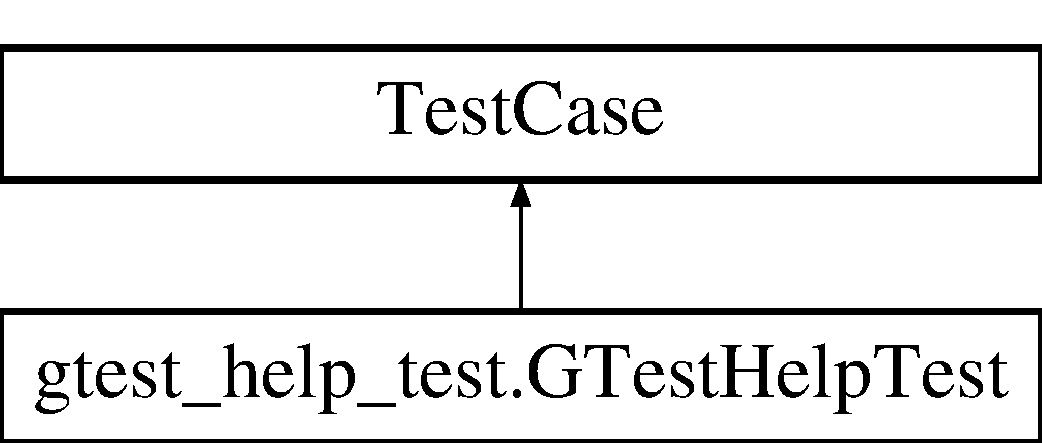
\includegraphics[height=2.000000cm]{classgtest__help__test_1_1_g_test_help_test}
\end{center}
\end{figure}
\subsection*{Public Member Functions}
\begin{DoxyCompactItemize}
\item 
def \mbox{\hyperlink{classgtest__help__test_1_1_g_test_help_test_a26cc1a64bd67278252ebfcd0ac0dca0c}{Test\+Help\+Flag}} (self, flag)
\item 
def \mbox{\hyperlink{classgtest__help__test_1_1_g_test_help_test_a03ffa91ecf6193ed2ed80b53933112ab}{Test\+Non\+Help\+Flag}} (self, flag)
\item 
\mbox{\Hypertarget{classgtest__help__test_1_1_g_test_help_test_ad91b46ad4506ff52b337b63f6b6c2ad1}\label{classgtest__help__test_1_1_g_test_help_test_ad91b46ad4506ff52b337b63f6b6c2ad1}} 
def {\bfseries test\+Prints\+Help\+With\+Full\+Flag} (self)
\item 
\mbox{\Hypertarget{classgtest__help__test_1_1_g_test_help_test_a3dd96058d093a89350769b4e2cc36563}\label{classgtest__help__test_1_1_g_test_help_test_a3dd96058d093a89350769b4e2cc36563}} 
def {\bfseries test\+Prints\+Help\+With\+Short\+Flag} (self)
\item 
\mbox{\Hypertarget{classgtest__help__test_1_1_g_test_help_test_aafd4d1857c2538c8b1f7cc5a5d1e38b4}\label{classgtest__help__test_1_1_g_test_help_test_aafd4d1857c2538c8b1f7cc5a5d1e38b4}} 
def {\bfseries test\+Prints\+Help\+With\+Question\+Flag} (self)
\item 
\mbox{\Hypertarget{classgtest__help__test_1_1_g_test_help_test_a7be99cd30193e2eecf79f9d65f561afc}\label{classgtest__help__test_1_1_g_test_help_test_a7be99cd30193e2eecf79f9d65f561afc}} 
def {\bfseries test\+Prints\+Help\+With\+Windows\+Style\+Question\+Flag} (self)
\item 
\mbox{\Hypertarget{classgtest__help__test_1_1_g_test_help_test_a701abb8f34df726b9129d7654cb32066}\label{classgtest__help__test_1_1_g_test_help_test_a701abb8f34df726b9129d7654cb32066}} 
def {\bfseries test\+Prints\+Help\+With\+Unrecognized\+Google\+Test\+Flag} (self)
\item 
\mbox{\Hypertarget{classgtest__help__test_1_1_g_test_help_test_ab8d379bbb0da7403ced599f4ee498728}\label{classgtest__help__test_1_1_g_test_help_test_ab8d379bbb0da7403ced599f4ee498728}} 
def {\bfseries test\+Prints\+Help\+With\+Incorrect\+Flag\+Style} (self)
\item 
def \mbox{\hyperlink{classgtest__help__test_1_1_g_test_help_test_ae7831f92e8e3763c07afb908915b3d20}{test\+Runs\+Tests\+Without\+Help\+Flag}} (self)
\item 
def \mbox{\hyperlink{classgtest__help__test_1_1_g_test_help_test_a0ebec2e3154d22a63e362d2196f9c638}{test\+Runs\+Tests\+With\+Gtest\+Internal\+Flag}} (self)
\end{DoxyCompactItemize}


\subsection{Detailed Description}
\begin{DoxyVerb}Tests the --help flag and its equivalent forms.\end{DoxyVerb}
 

\subsection{Member Function Documentation}
\mbox{\Hypertarget{classgtest__help__test_1_1_g_test_help_test_a26cc1a64bd67278252ebfcd0ac0dca0c}\label{classgtest__help__test_1_1_g_test_help_test_a26cc1a64bd67278252ebfcd0ac0dca0c}} 
\index{gtest\+\_\+help\+\_\+test\+::\+G\+Test\+Help\+Test@{gtest\+\_\+help\+\_\+test\+::\+G\+Test\+Help\+Test}!Test\+Help\+Flag@{Test\+Help\+Flag}}
\index{Test\+Help\+Flag@{Test\+Help\+Flag}!gtest\+\_\+help\+\_\+test\+::\+G\+Test\+Help\+Test@{gtest\+\_\+help\+\_\+test\+::\+G\+Test\+Help\+Test}}
\subsubsection{\texorpdfstring{Test\+Help\+Flag()}{TestHelpFlag()}}
{\footnotesize\ttfamily def gtest\+\_\+help\+\_\+test.\+G\+Test\+Help\+Test.\+Test\+Help\+Flag (\begin{DoxyParamCaption}\item[{}]{self,  }\item[{}]{flag }\end{DoxyParamCaption})}

\begin{DoxyVerb}Verifies correct behavior when help flag is specified.

The right message must be printed and the tests must
skipped when the given flag is specified.

Args:
  flag:  A flag to pass to the binary or None.
\end{DoxyVerb}
 \mbox{\Hypertarget{classgtest__help__test_1_1_g_test_help_test_a03ffa91ecf6193ed2ed80b53933112ab}\label{classgtest__help__test_1_1_g_test_help_test_a03ffa91ecf6193ed2ed80b53933112ab}} 
\index{gtest\+\_\+help\+\_\+test\+::\+G\+Test\+Help\+Test@{gtest\+\_\+help\+\_\+test\+::\+G\+Test\+Help\+Test}!Test\+Non\+Help\+Flag@{Test\+Non\+Help\+Flag}}
\index{Test\+Non\+Help\+Flag@{Test\+Non\+Help\+Flag}!gtest\+\_\+help\+\_\+test\+::\+G\+Test\+Help\+Test@{gtest\+\_\+help\+\_\+test\+::\+G\+Test\+Help\+Test}}
\subsubsection{\texorpdfstring{Test\+Non\+Help\+Flag()}{TestNonHelpFlag()}}
{\footnotesize\ttfamily def gtest\+\_\+help\+\_\+test.\+G\+Test\+Help\+Test.\+Test\+Non\+Help\+Flag (\begin{DoxyParamCaption}\item[{}]{self,  }\item[{}]{flag }\end{DoxyParamCaption})}

\begin{DoxyVerb}Verifies correct behavior when no help flag is specified.

Verifies that when no help flag is specified, the tests are run
and the help message is not printed.

Args:
  flag:  A flag to pass to the binary or None.
\end{DoxyVerb}
 \mbox{\Hypertarget{classgtest__help__test_1_1_g_test_help_test_a0ebec2e3154d22a63e362d2196f9c638}\label{classgtest__help__test_1_1_g_test_help_test_a0ebec2e3154d22a63e362d2196f9c638}} 
\index{gtest\+\_\+help\+\_\+test\+::\+G\+Test\+Help\+Test@{gtest\+\_\+help\+\_\+test\+::\+G\+Test\+Help\+Test}!test\+Runs\+Tests\+With\+Gtest\+Internal\+Flag@{test\+Runs\+Tests\+With\+Gtest\+Internal\+Flag}}
\index{test\+Runs\+Tests\+With\+Gtest\+Internal\+Flag@{test\+Runs\+Tests\+With\+Gtest\+Internal\+Flag}!gtest\+\_\+help\+\_\+test\+::\+G\+Test\+Help\+Test@{gtest\+\_\+help\+\_\+test\+::\+G\+Test\+Help\+Test}}
\subsubsection{\texorpdfstring{test\+Runs\+Tests\+With\+Gtest\+Internal\+Flag()}{testRunsTestsWithGtestInternalFlag()}}
{\footnotesize\ttfamily def gtest\+\_\+help\+\_\+test.\+G\+Test\+Help\+Test.\+test\+Runs\+Tests\+With\+Gtest\+Internal\+Flag (\begin{DoxyParamCaption}\item[{}]{self }\end{DoxyParamCaption})}

\begin{DoxyVerb}Verifies that the tests are run and no help message is printed when
a flag starting with Google Test prefix and 'internal_' is supplied.\end{DoxyVerb}
 \mbox{\Hypertarget{classgtest__help__test_1_1_g_test_help_test_ae7831f92e8e3763c07afb908915b3d20}\label{classgtest__help__test_1_1_g_test_help_test_ae7831f92e8e3763c07afb908915b3d20}} 
\index{gtest\+\_\+help\+\_\+test\+::\+G\+Test\+Help\+Test@{gtest\+\_\+help\+\_\+test\+::\+G\+Test\+Help\+Test}!test\+Runs\+Tests\+Without\+Help\+Flag@{test\+Runs\+Tests\+Without\+Help\+Flag}}
\index{test\+Runs\+Tests\+Without\+Help\+Flag@{test\+Runs\+Tests\+Without\+Help\+Flag}!gtest\+\_\+help\+\_\+test\+::\+G\+Test\+Help\+Test@{gtest\+\_\+help\+\_\+test\+::\+G\+Test\+Help\+Test}}
\subsubsection{\texorpdfstring{test\+Runs\+Tests\+Without\+Help\+Flag()}{testRunsTestsWithoutHelpFlag()}}
{\footnotesize\ttfamily def gtest\+\_\+help\+\_\+test.\+G\+Test\+Help\+Test.\+test\+Runs\+Tests\+Without\+Help\+Flag (\begin{DoxyParamCaption}\item[{}]{self }\end{DoxyParamCaption})}

\begin{DoxyVerb}Verifies that when no help flag is specified, the tests are run
and the help message is not printed.\end{DoxyVerb}
 

The documentation for this class was generated from the following file\+:\begin{DoxyCompactItemize}
\item 
/\+Users/fjp/git/bachelor/bachelor-\/master\+\_\+updated\+\_\+vfinal/googletest-\/1.\+8.\+0/googletest/test/gtest\+\_\+help\+\_\+test.\+py\end{DoxyCompactItemize}

\hypertarget{classgtest__list__tests__unittest_1_1_g_test_list_tests_unit_test}{}\section{gtest\+\_\+list\+\_\+tests\+\_\+unittest.\+G\+Test\+List\+Tests\+Unit\+Test Class Reference}
\label{classgtest__list__tests__unittest_1_1_g_test_list_tests_unit_test}\index{gtest\+\_\+list\+\_\+tests\+\_\+unittest.\+G\+Test\+List\+Tests\+Unit\+Test@{gtest\+\_\+list\+\_\+tests\+\_\+unittest.\+G\+Test\+List\+Tests\+Unit\+Test}}
Inheritance diagram for gtest\+\_\+list\+\_\+tests\+\_\+unittest.\+G\+Test\+List\+Tests\+Unit\+Test\+:\begin{figure}[H]
\begin{center}
\leavevmode
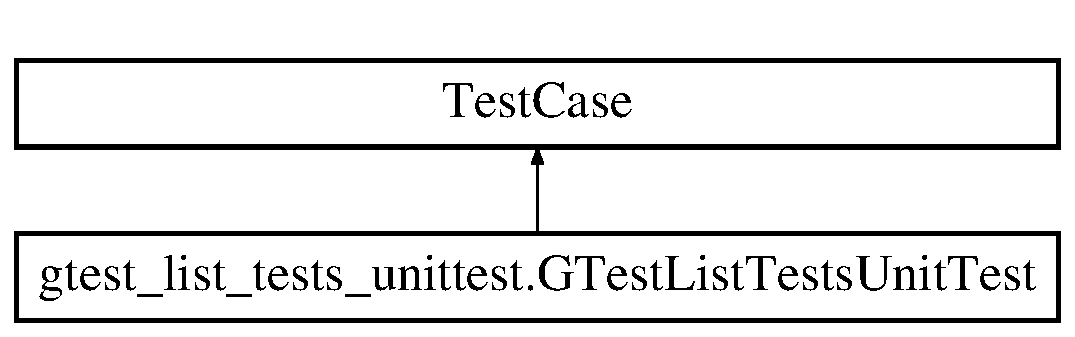
\includegraphics[height=2.000000cm]{classgtest__list__tests__unittest_1_1_g_test_list_tests_unit_test}
\end{center}
\end{figure}
\subsection*{Public Member Functions}
\begin{DoxyCompactItemize}
\item 
def \mbox{\hyperlink{classgtest__list__tests__unittest_1_1_g_test_list_tests_unit_test_a965601cd1882fdeca94d2461bd033c40}{Run\+And\+Verify}} (self, flag\+\_\+value, expected\+\_\+output\+\_\+re, other\+\_\+flag)
\item 
def \mbox{\hyperlink{classgtest__list__tests__unittest_1_1_g_test_list_tests_unit_test_a4168d086b7ec31f86ab548b6fd79b27e}{test\+Default\+Behavior}} (self)
\item 
def \mbox{\hyperlink{classgtest__list__tests__unittest_1_1_g_test_list_tests_unit_test_a6d3e8738bd4b7494867cac464d342944}{test\+Flag}} (self)
\item 
def \mbox{\hyperlink{classgtest__list__tests__unittest_1_1_g_test_list_tests_unit_test_ae1ccba3f21c8e25968834607f7db2b10}{test\+Override\+Non\+Filter\+Flags}} (self)
\item 
def \mbox{\hyperlink{classgtest__list__tests__unittest_1_1_g_test_list_tests_unit_test_ac5bef6c9fb78b8eef84427de811fd70f}{test\+With\+Filter\+Flags}} (self)
\end{DoxyCompactItemize}


\subsection{Detailed Description}
\begin{DoxyVerb}Tests using the --gtest_list_tests flag to list all tests.\end{DoxyVerb}
 

\subsection{Member Function Documentation}
\mbox{\Hypertarget{classgtest__list__tests__unittest_1_1_g_test_list_tests_unit_test_a965601cd1882fdeca94d2461bd033c40}\label{classgtest__list__tests__unittest_1_1_g_test_list_tests_unit_test_a965601cd1882fdeca94d2461bd033c40}} 
\index{gtest\+\_\+list\+\_\+tests\+\_\+unittest\+::\+G\+Test\+List\+Tests\+Unit\+Test@{gtest\+\_\+list\+\_\+tests\+\_\+unittest\+::\+G\+Test\+List\+Tests\+Unit\+Test}!Run\+And\+Verify@{Run\+And\+Verify}}
\index{Run\+And\+Verify@{Run\+And\+Verify}!gtest\+\_\+list\+\_\+tests\+\_\+unittest\+::\+G\+Test\+List\+Tests\+Unit\+Test@{gtest\+\_\+list\+\_\+tests\+\_\+unittest\+::\+G\+Test\+List\+Tests\+Unit\+Test}}
\subsubsection{\texorpdfstring{Run\+And\+Verify()}{RunAndVerify()}}
{\footnotesize\ttfamily def gtest\+\_\+list\+\_\+tests\+\_\+unittest.\+G\+Test\+List\+Tests\+Unit\+Test.\+Run\+And\+Verify (\begin{DoxyParamCaption}\item[{}]{self,  }\item[{}]{flag\+\_\+value,  }\item[{}]{expected\+\_\+output\+\_\+re,  }\item[{}]{other\+\_\+flag }\end{DoxyParamCaption})}

\begin{DoxyVerb}Runs gtest_list_tests_unittest_ and verifies that it prints
the correct tests.

Args:
  flag_value:         value of the --gtest_list_tests flag;
                  None if the flag should not be present.
  expected_output_re: regular expression that matches the expected
                  output after running command;
  other_flag:         a different flag to be passed to command
                  along with gtest_list_tests;
                  None if the flag should not be present.
\end{DoxyVerb}
 \mbox{\Hypertarget{classgtest__list__tests__unittest_1_1_g_test_list_tests_unit_test_a4168d086b7ec31f86ab548b6fd79b27e}\label{classgtest__list__tests__unittest_1_1_g_test_list_tests_unit_test_a4168d086b7ec31f86ab548b6fd79b27e}} 
\index{gtest\+\_\+list\+\_\+tests\+\_\+unittest\+::\+G\+Test\+List\+Tests\+Unit\+Test@{gtest\+\_\+list\+\_\+tests\+\_\+unittest\+::\+G\+Test\+List\+Tests\+Unit\+Test}!test\+Default\+Behavior@{test\+Default\+Behavior}}
\index{test\+Default\+Behavior@{test\+Default\+Behavior}!gtest\+\_\+list\+\_\+tests\+\_\+unittest\+::\+G\+Test\+List\+Tests\+Unit\+Test@{gtest\+\_\+list\+\_\+tests\+\_\+unittest\+::\+G\+Test\+List\+Tests\+Unit\+Test}}
\subsubsection{\texorpdfstring{test\+Default\+Behavior()}{testDefaultBehavior()}}
{\footnotesize\ttfamily def gtest\+\_\+list\+\_\+tests\+\_\+unittest.\+G\+Test\+List\+Tests\+Unit\+Test.\+test\+Default\+Behavior (\begin{DoxyParamCaption}\item[{}]{self }\end{DoxyParamCaption})}

\begin{DoxyVerb}Tests the behavior of the default mode.\end{DoxyVerb}
 \mbox{\Hypertarget{classgtest__list__tests__unittest_1_1_g_test_list_tests_unit_test_a6d3e8738bd4b7494867cac464d342944}\label{classgtest__list__tests__unittest_1_1_g_test_list_tests_unit_test_a6d3e8738bd4b7494867cac464d342944}} 
\index{gtest\+\_\+list\+\_\+tests\+\_\+unittest\+::\+G\+Test\+List\+Tests\+Unit\+Test@{gtest\+\_\+list\+\_\+tests\+\_\+unittest\+::\+G\+Test\+List\+Tests\+Unit\+Test}!test\+Flag@{test\+Flag}}
\index{test\+Flag@{test\+Flag}!gtest\+\_\+list\+\_\+tests\+\_\+unittest\+::\+G\+Test\+List\+Tests\+Unit\+Test@{gtest\+\_\+list\+\_\+tests\+\_\+unittest\+::\+G\+Test\+List\+Tests\+Unit\+Test}}
\subsubsection{\texorpdfstring{test\+Flag()}{testFlag()}}
{\footnotesize\ttfamily def gtest\+\_\+list\+\_\+tests\+\_\+unittest.\+G\+Test\+List\+Tests\+Unit\+Test.\+test\+Flag (\begin{DoxyParamCaption}\item[{}]{self }\end{DoxyParamCaption})}

\begin{DoxyVerb}Tests using the --gtest_list_tests flag.\end{DoxyVerb}
 \mbox{\Hypertarget{classgtest__list__tests__unittest_1_1_g_test_list_tests_unit_test_ae1ccba3f21c8e25968834607f7db2b10}\label{classgtest__list__tests__unittest_1_1_g_test_list_tests_unit_test_ae1ccba3f21c8e25968834607f7db2b10}} 
\index{gtest\+\_\+list\+\_\+tests\+\_\+unittest\+::\+G\+Test\+List\+Tests\+Unit\+Test@{gtest\+\_\+list\+\_\+tests\+\_\+unittest\+::\+G\+Test\+List\+Tests\+Unit\+Test}!test\+Override\+Non\+Filter\+Flags@{test\+Override\+Non\+Filter\+Flags}}
\index{test\+Override\+Non\+Filter\+Flags@{test\+Override\+Non\+Filter\+Flags}!gtest\+\_\+list\+\_\+tests\+\_\+unittest\+::\+G\+Test\+List\+Tests\+Unit\+Test@{gtest\+\_\+list\+\_\+tests\+\_\+unittest\+::\+G\+Test\+List\+Tests\+Unit\+Test}}
\subsubsection{\texorpdfstring{test\+Override\+Non\+Filter\+Flags()}{testOverrideNonFilterFlags()}}
{\footnotesize\ttfamily def gtest\+\_\+list\+\_\+tests\+\_\+unittest.\+G\+Test\+List\+Tests\+Unit\+Test.\+test\+Override\+Non\+Filter\+Flags (\begin{DoxyParamCaption}\item[{}]{self }\end{DoxyParamCaption})}

\begin{DoxyVerb}Tests that --gtest_list_tests overrides the non-filter flags.\end{DoxyVerb}
 \mbox{\Hypertarget{classgtest__list__tests__unittest_1_1_g_test_list_tests_unit_test_ac5bef6c9fb78b8eef84427de811fd70f}\label{classgtest__list__tests__unittest_1_1_g_test_list_tests_unit_test_ac5bef6c9fb78b8eef84427de811fd70f}} 
\index{gtest\+\_\+list\+\_\+tests\+\_\+unittest\+::\+G\+Test\+List\+Tests\+Unit\+Test@{gtest\+\_\+list\+\_\+tests\+\_\+unittest\+::\+G\+Test\+List\+Tests\+Unit\+Test}!test\+With\+Filter\+Flags@{test\+With\+Filter\+Flags}}
\index{test\+With\+Filter\+Flags@{test\+With\+Filter\+Flags}!gtest\+\_\+list\+\_\+tests\+\_\+unittest\+::\+G\+Test\+List\+Tests\+Unit\+Test@{gtest\+\_\+list\+\_\+tests\+\_\+unittest\+::\+G\+Test\+List\+Tests\+Unit\+Test}}
\subsubsection{\texorpdfstring{test\+With\+Filter\+Flags()}{testWithFilterFlags()}}
{\footnotesize\ttfamily def gtest\+\_\+list\+\_\+tests\+\_\+unittest.\+G\+Test\+List\+Tests\+Unit\+Test.\+test\+With\+Filter\+Flags (\begin{DoxyParamCaption}\item[{}]{self }\end{DoxyParamCaption})}

\begin{DoxyVerb}Tests that --gtest_list_tests takes into account the
--gtest_filter flag.\end{DoxyVerb}
 

The documentation for this class was generated from the following file\+:\begin{DoxyCompactItemize}
\item 
/\+Users/fjp/git/bachelor/bachelor-\/master\+\_\+updated\+\_\+vfinal/googletest-\/1.\+8.\+0/googletest/test/gtest\+\_\+list\+\_\+tests\+\_\+unittest.\+py\end{DoxyCompactItemize}

\hypertarget{classtesting_1_1internal_1_1_g_test_log}{}\section{testing\+:\+:internal\+:\+:G\+Test\+Log Class Reference}
\label{classtesting_1_1internal_1_1_g_test_log}\index{testing\+::internal\+::\+G\+Test\+Log@{testing\+::internal\+::\+G\+Test\+Log}}
\subsection*{Public Member Functions}
\begin{DoxyCompactItemize}
\item 
\mbox{\Hypertarget{classtesting_1_1internal_1_1_g_test_log_a364691bf972983a59cfa2891062a64af}\label{classtesting_1_1internal_1_1_g_test_log_a364691bf972983a59cfa2891062a64af}} 
{\bfseries G\+Test\+Log} (G\+Test\+Log\+Severity severity, const char $\ast$file, int line)
\item 
\mbox{\Hypertarget{classtesting_1_1internal_1_1_g_test_log_aebb92e67d98eca69f0347d5121dab27a}\label{classtesting_1_1internal_1_1_g_test_log_aebb92e67d98eca69f0347d5121dab27a}} 
\+::std\+::ostream \& {\bfseries Get\+Stream} ()
\end{DoxyCompactItemize}


The documentation for this class was generated from the following files\+:\begin{DoxyCompactItemize}
\item 
/\+Users/fjp/git/bachelor/bachelor-\/master\+\_\+updated\+\_\+vfinal/googletest-\/1.\+8.\+0/googletest/include/gtest/internal/gtest-\/port.\+h\item 
/\+Users/fjp/git/bachelor/bachelor-\/master\+\_\+updated\+\_\+vfinal/googletest-\/1.\+8.\+0/googletest/src/gtest-\/port.\+cc\end{DoxyCompactItemize}

\hypertarget{classtesting_1_1internal_1_1_g_test_mutex_lock}{}\section{testing\+:\+:internal\+:\+:G\+Test\+Mutex\+Lock Class Reference}
\label{classtesting_1_1internal_1_1_g_test_mutex_lock}\index{testing\+::internal\+::\+G\+Test\+Mutex\+Lock@{testing\+::internal\+::\+G\+Test\+Mutex\+Lock}}
\subsection*{Public Member Functions}
\begin{DoxyCompactItemize}
\item 
\mbox{\Hypertarget{classtesting_1_1internal_1_1_g_test_mutex_lock_a77e3cba326d5356b4a1dea3790559c26}\label{classtesting_1_1internal_1_1_g_test_mutex_lock_a77e3cba326d5356b4a1dea3790559c26}} 
{\bfseries G\+Test\+Mutex\+Lock} (\mbox{\hyperlink{classtesting_1_1internal_1_1_mutex}{Mutex}} $\ast$)
\end{DoxyCompactItemize}


The documentation for this class was generated from the following file\+:\begin{DoxyCompactItemize}
\item 
/\+Users/fjp/git/bachelor/bachelor-\/master\+\_\+updated\+\_\+vfinal/googletest-\/1.\+8.\+0/googletest/include/gtest/internal/gtest-\/port.\+h\end{DoxyCompactItemize}

\hypertarget{classgtest__output__test_1_1_g_test_output_test}{}\section{gtest\+\_\+output\+\_\+test.\+G\+Test\+Output\+Test Class Reference}
\label{classgtest__output__test_1_1_g_test_output_test}\index{gtest\+\_\+output\+\_\+test.\+G\+Test\+Output\+Test@{gtest\+\_\+output\+\_\+test.\+G\+Test\+Output\+Test}}
Inheritance diagram for gtest\+\_\+output\+\_\+test.\+G\+Test\+Output\+Test\+:\begin{figure}[H]
\begin{center}
\leavevmode
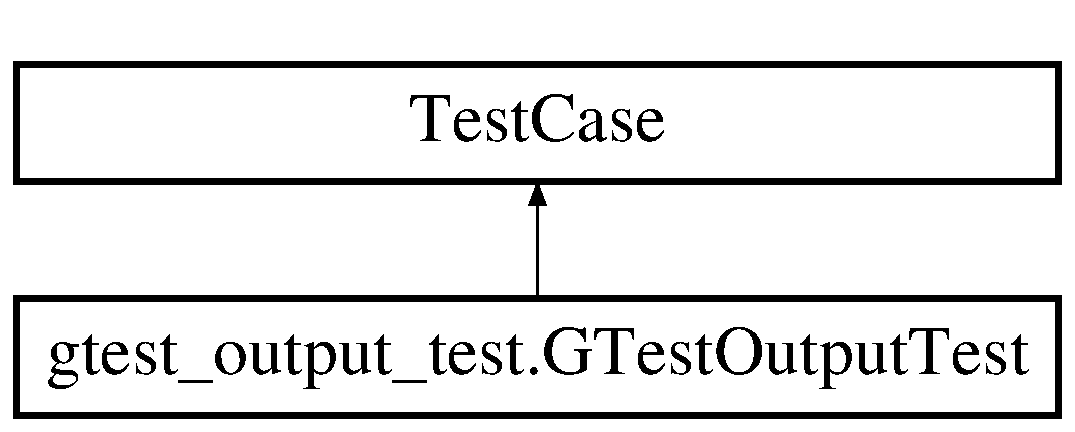
\includegraphics[height=2.000000cm]{classgtest__output__test_1_1_g_test_output_test}
\end{center}
\end{figure}
\subsection*{Public Member Functions}
\begin{DoxyCompactItemize}
\item 
\mbox{\Hypertarget{classgtest__output__test_1_1_g_test_output_test_a63f62268f795adfc5ca91514dbec2873}\label{classgtest__output__test_1_1_g_test_output_test_a63f62268f795adfc5ca91514dbec2873}} 
def {\bfseries Remove\+Unsupported\+Tests} (self, test\+\_\+output)
\item 
\mbox{\Hypertarget{classgtest__output__test_1_1_g_test_output_test_a1e6b96f68c5bcb8271de3208fa7f9f64}\label{classgtest__output__test_1_1_g_test_output_test_a1e6b96f68c5bcb8271de3208fa7f9f64}} 
def {\bfseries test\+Output} (self)
\end{DoxyCompactItemize}


The documentation for this class was generated from the following file\+:\begin{DoxyCompactItemize}
\item 
/\+Users/fjp/git/bachelor/bachelor-\/master\+\_\+updated\+\_\+vfinal/googletest-\/1.\+8.\+0/googletest/test/gtest\+\_\+output\+\_\+test.\+py\end{DoxyCompactItemize}

\hypertarget{classgtest__shuffle__test_1_1_g_test_shuffle_unit_test}{}\section{gtest\+\_\+shuffle\+\_\+test.\+G\+Test\+Shuffle\+Unit\+Test Class Reference}
\label{classgtest__shuffle__test_1_1_g_test_shuffle_unit_test}\index{gtest\+\_\+shuffle\+\_\+test.\+G\+Test\+Shuffle\+Unit\+Test@{gtest\+\_\+shuffle\+\_\+test.\+G\+Test\+Shuffle\+Unit\+Test}}
Inheritance diagram for gtest\+\_\+shuffle\+\_\+test.\+G\+Test\+Shuffle\+Unit\+Test\+:\begin{figure}[H]
\begin{center}
\leavevmode
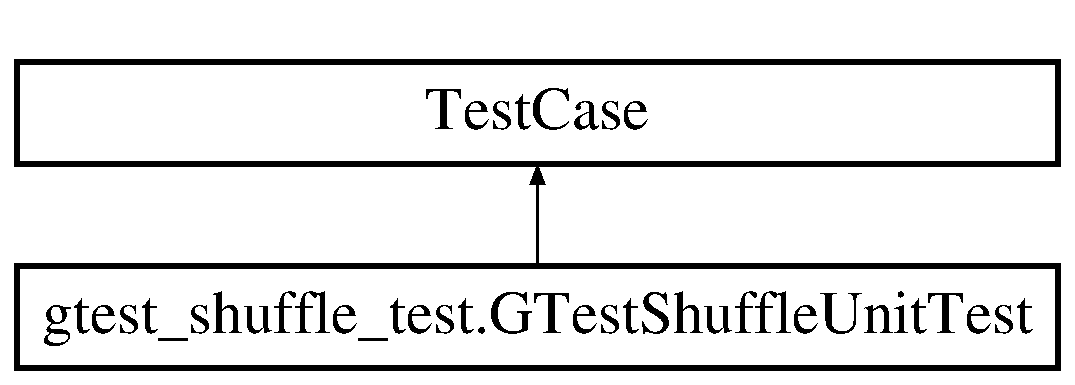
\includegraphics[height=2.000000cm]{classgtest__shuffle__test_1_1_g_test_shuffle_unit_test}
\end{center}
\end{figure}
\subsection*{Public Member Functions}
\begin{DoxyCompactItemize}
\item 
\mbox{\Hypertarget{classgtest__shuffle__test_1_1_g_test_shuffle_unit_test_adf9841ae9c86eaafc3c3f7c9690c7bd8}\label{classgtest__shuffle__test_1_1_g_test_shuffle_unit_test_adf9841ae9c86eaafc3c3f7c9690c7bd8}} 
def {\bfseries set\+Up} (self)
\item 
\mbox{\Hypertarget{classgtest__shuffle__test_1_1_g_test_shuffle_unit_test_aafc33d6129c37043ef5c95dbe766a8db}\label{classgtest__shuffle__test_1_1_g_test_shuffle_unit_test_aafc33d6129c37043ef5c95dbe766a8db}} 
def {\bfseries test\+Shuffle\+Preserves\+Number\+Of\+Tests} (self)
\item 
\mbox{\Hypertarget{classgtest__shuffle__test_1_1_g_test_shuffle_unit_test_a0ba25ee553b62281e16b6a28873abc01}\label{classgtest__shuffle__test_1_1_g_test_shuffle_unit_test_a0ba25ee553b62281e16b6a28873abc01}} 
def {\bfseries test\+Shuffle\+Changes\+Test\+Order} (self)
\item 
\mbox{\Hypertarget{classgtest__shuffle__test_1_1_g_test_shuffle_unit_test_a8a82320ea310d1e3660bef2efb665bd2}\label{classgtest__shuffle__test_1_1_g_test_shuffle_unit_test_a8a82320ea310d1e3660bef2efb665bd2}} 
def {\bfseries test\+Shuffle\+Changes\+Test\+Case\+Order} (self)
\item 
\mbox{\Hypertarget{classgtest__shuffle__test_1_1_g_test_shuffle_unit_test_a7537baa50e9e14b430fb80eaf4ea18f6}\label{classgtest__shuffle__test_1_1_g_test_shuffle_unit_test_a7537baa50e9e14b430fb80eaf4ea18f6}} 
def {\bfseries test\+Shuffle\+Does\+Not\+Repeat\+Test} (self)
\item 
\mbox{\Hypertarget{classgtest__shuffle__test_1_1_g_test_shuffle_unit_test_aeea745f7ce2ab19a067c5cde6e083ba7}\label{classgtest__shuffle__test_1_1_g_test_shuffle_unit_test_aeea745f7ce2ab19a067c5cde6e083ba7}} 
def {\bfseries test\+Shuffle\+Does\+Not\+Create\+New\+Test} (self)
\item 
\mbox{\Hypertarget{classgtest__shuffle__test_1_1_g_test_shuffle_unit_test_ab9e25e62817f7cdbd32833f9b2be5794}\label{classgtest__shuffle__test_1_1_g_test_shuffle_unit_test_ab9e25e62817f7cdbd32833f9b2be5794}} 
def {\bfseries test\+Shuffle\+Includes\+All\+Tests} (self)
\item 
\mbox{\Hypertarget{classgtest__shuffle__test_1_1_g_test_shuffle_unit_test_a6fa91b262595e35bd3e9b52e188dc634}\label{classgtest__shuffle__test_1_1_g_test_shuffle_unit_test_a6fa91b262595e35bd3e9b52e188dc634}} 
def {\bfseries test\+Shuffle\+Leaves\+Death\+Tests\+At\+Front} (self)
\item 
\mbox{\Hypertarget{classgtest__shuffle__test_1_1_g_test_shuffle_unit_test_a34bfc9696191f4c2782327e1e35ae902}\label{classgtest__shuffle__test_1_1_g_test_shuffle_unit_test_a34bfc9696191f4c2782327e1e35ae902}} 
def {\bfseries test\+Shuffle\+Does\+Not\+Interleave\+Test\+Cases} (self)
\item 
\mbox{\Hypertarget{classgtest__shuffle__test_1_1_g_test_shuffle_unit_test_a77b83a9870ad8d68524e1177f5320fb0}\label{classgtest__shuffle__test_1_1_g_test_shuffle_unit_test_a77b83a9870ad8d68524e1177f5320fb0}} 
def {\bfseries test\+Shuffle\+Restores\+Order\+After\+Each\+Iteration} (self)
\item 
\mbox{\Hypertarget{classgtest__shuffle__test_1_1_g_test_shuffle_unit_test_ada78bae27e0d82d07bd663d53a36552b}\label{classgtest__shuffle__test_1_1_g_test_shuffle_unit_test_ada78bae27e0d82d07bd663d53a36552b}} 
def {\bfseries test\+Shuffle\+Generates\+New\+Order\+In\+Each\+Iteration} (self)
\item 
\mbox{\Hypertarget{classgtest__shuffle__test_1_1_g_test_shuffle_unit_test_abd33c5ef01ce6d1d025ebcc816d47c19}\label{classgtest__shuffle__test_1_1_g_test_shuffle_unit_test_abd33c5ef01ce6d1d025ebcc816d47c19}} 
def {\bfseries test\+Shuffle\+Sharded\+Tests\+Preserves\+Partition} (self)
\end{DoxyCompactItemize}


\subsection{Detailed Description}
\begin{DoxyVerb}Tests test shuffling.\end{DoxyVerb}
 

The documentation for this class was generated from the following file\+:\begin{DoxyCompactItemize}
\item 
/\+Users/fjp/git/bachelor/bachelor-\/master\+\_\+updated\+\_\+vfinal/googletest-\/1.\+8.\+0/googletest/test/gtest\+\_\+shuffle\+\_\+test.\+py\end{DoxyCompactItemize}

\hypertarget{classgtest__uninitialized__test_1_1_g_test_uninitialized_test}{}\section{gtest\+\_\+uninitialized\+\_\+test.\+G\+Test\+Uninitialized\+Test Class Reference}
\label{classgtest__uninitialized__test_1_1_g_test_uninitialized_test}\index{gtest\+\_\+uninitialized\+\_\+test.\+G\+Test\+Uninitialized\+Test@{gtest\+\_\+uninitialized\+\_\+test.\+G\+Test\+Uninitialized\+Test}}
Inheritance diagram for gtest\+\_\+uninitialized\+\_\+test.\+G\+Test\+Uninitialized\+Test\+:\begin{figure}[H]
\begin{center}
\leavevmode
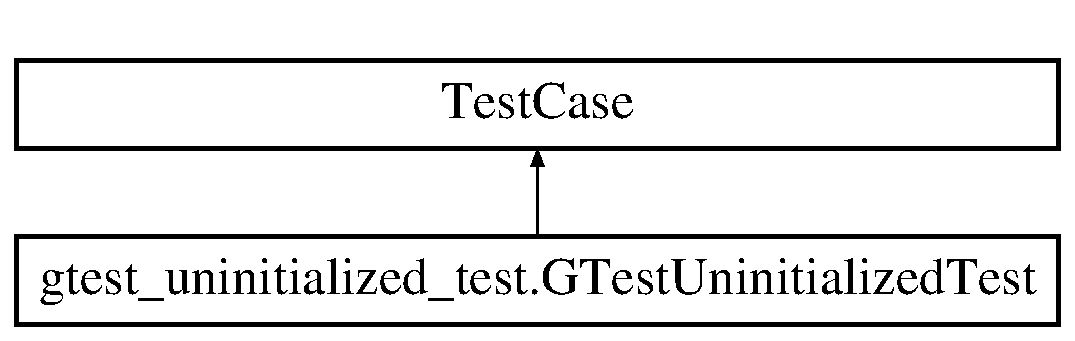
\includegraphics[height=2.000000cm]{classgtest__uninitialized__test_1_1_g_test_uninitialized_test}
\end{center}
\end{figure}
\subsection*{Public Member Functions}
\begin{DoxyCompactItemize}
\item 
\mbox{\Hypertarget{classgtest__uninitialized__test_1_1_g_test_uninitialized_test_ace4bbad0abec476b03a91bb453e6451c}\label{classgtest__uninitialized__test_1_1_g_test_uninitialized_test_ace4bbad0abec476b03a91bb453e6451c}} 
def {\bfseries test\+Exit\+Code\+And\+Output} (self)
\end{DoxyCompactItemize}


The documentation for this class was generated from the following file\+:\begin{DoxyCompactItemize}
\item 
/\+Users/fjp/git/bachelor/bachelor-\/master\+\_\+updated\+\_\+vfinal/googletest-\/1.\+8.\+0/googletest/test/gtest\+\_\+uninitialized\+\_\+test.\+py\end{DoxyCompactItemize}

\hypertarget{classgtest__xml__outfiles__test_1_1_g_test_x_m_l_out_files_test}{}\section{gtest\+\_\+xml\+\_\+outfiles\+\_\+test.\+G\+Test\+X\+M\+L\+Out\+Files\+Test Class Reference}
\label{classgtest__xml__outfiles__test_1_1_g_test_x_m_l_out_files_test}\index{gtest\+\_\+xml\+\_\+outfiles\+\_\+test.\+G\+Test\+X\+M\+L\+Out\+Files\+Test@{gtest\+\_\+xml\+\_\+outfiles\+\_\+test.\+G\+Test\+X\+M\+L\+Out\+Files\+Test}}
Inheritance diagram for gtest\+\_\+xml\+\_\+outfiles\+\_\+test.\+G\+Test\+X\+M\+L\+Out\+Files\+Test\+:\begin{figure}[H]
\begin{center}
\leavevmode
\includegraphics[height=3.000000cm]{classgtest__xml__outfiles__test_1_1_g_test_x_m_l_out_files_test}
\end{center}
\end{figure}
\subsection*{Public Member Functions}
\begin{DoxyCompactItemize}
\item 
\mbox{\Hypertarget{classgtest__xml__outfiles__test_1_1_g_test_x_m_l_out_files_test_a56550f293277d18c36e868a637fe1153}\label{classgtest__xml__outfiles__test_1_1_g_test_x_m_l_out_files_test_a56550f293277d18c36e868a637fe1153}} 
def {\bfseries set\+Up} (self)
\item 
\mbox{\Hypertarget{classgtest__xml__outfiles__test_1_1_g_test_x_m_l_out_files_test_a49d1d410370ba8a3cfcc281eaadb5706}\label{classgtest__xml__outfiles__test_1_1_g_test_x_m_l_out_files_test_a49d1d410370ba8a3cfcc281eaadb5706}} 
def {\bfseries tear\+Down} (self)
\item 
\mbox{\Hypertarget{classgtest__xml__outfiles__test_1_1_g_test_x_m_l_out_files_test_a503d2fbc9cd782ae57ac4307d2db43e1}\label{classgtest__xml__outfiles__test_1_1_g_test_x_m_l_out_files_test_a503d2fbc9cd782ae57ac4307d2db43e1}} 
def {\bfseries Delete\+Files\+And\+Dir} (self)
\item 
\mbox{\Hypertarget{classgtest__xml__outfiles__test_1_1_g_test_x_m_l_out_files_test_a034738bbc00ac46d00f183402c561228}\label{classgtest__xml__outfiles__test_1_1_g_test_x_m_l_out_files_test_a034738bbc00ac46d00f183402c561228}} 
def {\bfseries test\+Outfile1} (self)
\item 
\mbox{\Hypertarget{classgtest__xml__outfiles__test_1_1_g_test_x_m_l_out_files_test_a3c02687f092a482d0d0260c7ed94c618}\label{classgtest__xml__outfiles__test_1_1_g_test_x_m_l_out_files_test_a3c02687f092a482d0d0260c7ed94c618}} 
def {\bfseries test\+Outfile2} (self)
\end{DoxyCompactItemize}
\subsection*{Public Attributes}
\begin{DoxyCompactItemize}
\item 
\mbox{\Hypertarget{classgtest__xml__outfiles__test_1_1_g_test_x_m_l_out_files_test_aa5c31cd97047bc1d3060f4d27bc956a4}\label{classgtest__xml__outfiles__test_1_1_g_test_x_m_l_out_files_test_aa5c31cd97047bc1d3060f4d27bc956a4}} 
{\bfseries output\+\_\+dir\+\_\+}
\end{DoxyCompactItemize}
\subsection*{Additional Inherited Members}


\subsection{Detailed Description}
\begin{DoxyVerb}Unit test for Google Test's XML output functionality.\end{DoxyVerb}
 

The documentation for this class was generated from the following file\+:\begin{DoxyCompactItemize}
\item 
/\+Users/fjp/git/bachelor/bachelor-\/master\+\_\+updated\+\_\+vfinal/googletest-\/1.\+8.\+0/googletest/test/gtest\+\_\+xml\+\_\+outfiles\+\_\+test.\+py\end{DoxyCompactItemize}

\hypertarget{classgtest__xml__output__unittest_1_1_g_test_x_m_l_output_unit_test}{}\section{gtest\+\_\+xml\+\_\+output\+\_\+unittest.\+G\+Test\+X\+M\+L\+Output\+Unit\+Test Class Reference}
\label{classgtest__xml__output__unittest_1_1_g_test_x_m_l_output_unit_test}\index{gtest\+\_\+xml\+\_\+output\+\_\+unittest.\+G\+Test\+X\+M\+L\+Output\+Unit\+Test@{gtest\+\_\+xml\+\_\+output\+\_\+unittest.\+G\+Test\+X\+M\+L\+Output\+Unit\+Test}}
Inheritance diagram for gtest\+\_\+xml\+\_\+output\+\_\+unittest.\+G\+Test\+X\+M\+L\+Output\+Unit\+Test\+:\begin{figure}[H]
\begin{center}
\leavevmode
\includegraphics[height=3.000000cm]{classgtest__xml__output__unittest_1_1_g_test_x_m_l_output_unit_test}
\end{center}
\end{figure}
\subsection*{Public Member Functions}
\begin{DoxyCompactItemize}
\item 
def \mbox{\hyperlink{classgtest__xml__output__unittest_1_1_g_test_x_m_l_output_unit_test_a310c136c1eb2b421f57651a7d358b17a}{test\+Non\+Empty\+Xml\+Output}} (self)
\item 
def \mbox{\hyperlink{classgtest__xml__output__unittest_1_1_g_test_x_m_l_output_unit_test_a9602f91fe2e9d1e09171a032e94a5619}{test\+Empty\+Xml\+Output}} (self)
\item 
def \mbox{\hyperlink{classgtest__xml__output__unittest_1_1_g_test_x_m_l_output_unit_test_a828521a7ae57f650e1e9ca4beb34336a}{test\+Timestamp\+Value}} (self)
\item 
def \mbox{\hyperlink{classgtest__xml__output__unittest_1_1_g_test_x_m_l_output_unit_test_a01ca66e14468028e5c4eb809987113cf}{test\+Default\+Output\+File}} (self)
\item 
def \mbox{\hyperlink{classgtest__xml__output__unittest_1_1_g_test_x_m_l_output_unit_test_ac6df46d6831892e4c14dbdfae0049618}{test\+Suppressed\+Xml\+Output}} (self)
\item 
def \mbox{\hyperlink{classgtest__xml__output__unittest_1_1_g_test_x_m_l_output_unit_test_a572b6d49e8f4d646ebdadcced3d260ef}{test\+Filtered\+Test\+Xml\+Output}} (self)
\end{DoxyCompactItemize}
\subsection*{Additional Inherited Members}


\subsection{Detailed Description}
\begin{DoxyVerb}Unit test for Google Test's XML output functionality.
\end{DoxyVerb}
 

\subsection{Member Function Documentation}
\mbox{\Hypertarget{classgtest__xml__output__unittest_1_1_g_test_x_m_l_output_unit_test_a01ca66e14468028e5c4eb809987113cf}\label{classgtest__xml__output__unittest_1_1_g_test_x_m_l_output_unit_test_a01ca66e14468028e5c4eb809987113cf}} 
\index{gtest\+\_\+xml\+\_\+output\+\_\+unittest\+::\+G\+Test\+X\+M\+L\+Output\+Unit\+Test@{gtest\+\_\+xml\+\_\+output\+\_\+unittest\+::\+G\+Test\+X\+M\+L\+Output\+Unit\+Test}!test\+Default\+Output\+File@{test\+Default\+Output\+File}}
\index{test\+Default\+Output\+File@{test\+Default\+Output\+File}!gtest\+\_\+xml\+\_\+output\+\_\+unittest\+::\+G\+Test\+X\+M\+L\+Output\+Unit\+Test@{gtest\+\_\+xml\+\_\+output\+\_\+unittest\+::\+G\+Test\+X\+M\+L\+Output\+Unit\+Test}}
\subsubsection{\texorpdfstring{test\+Default\+Output\+File()}{testDefaultOutputFile()}}
{\footnotesize\ttfamily def gtest\+\_\+xml\+\_\+output\+\_\+unittest.\+G\+Test\+X\+M\+L\+Output\+Unit\+Test.\+test\+Default\+Output\+File (\begin{DoxyParamCaption}\item[{}]{self }\end{DoxyParamCaption})}

\begin{DoxyVerb}Confirms that Google Test produces an XML output file with the expected
default name if no name is explicitly specified.
\end{DoxyVerb}
 \mbox{\Hypertarget{classgtest__xml__output__unittest_1_1_g_test_x_m_l_output_unit_test_a9602f91fe2e9d1e09171a032e94a5619}\label{classgtest__xml__output__unittest_1_1_g_test_x_m_l_output_unit_test_a9602f91fe2e9d1e09171a032e94a5619}} 
\index{gtest\+\_\+xml\+\_\+output\+\_\+unittest\+::\+G\+Test\+X\+M\+L\+Output\+Unit\+Test@{gtest\+\_\+xml\+\_\+output\+\_\+unittest\+::\+G\+Test\+X\+M\+L\+Output\+Unit\+Test}!test\+Empty\+Xml\+Output@{test\+Empty\+Xml\+Output}}
\index{test\+Empty\+Xml\+Output@{test\+Empty\+Xml\+Output}!gtest\+\_\+xml\+\_\+output\+\_\+unittest\+::\+G\+Test\+X\+M\+L\+Output\+Unit\+Test@{gtest\+\_\+xml\+\_\+output\+\_\+unittest\+::\+G\+Test\+X\+M\+L\+Output\+Unit\+Test}}
\subsubsection{\texorpdfstring{test\+Empty\+Xml\+Output()}{testEmptyXmlOutput()}}
{\footnotesize\ttfamily def gtest\+\_\+xml\+\_\+output\+\_\+unittest.\+G\+Test\+X\+M\+L\+Output\+Unit\+Test.\+test\+Empty\+Xml\+Output (\begin{DoxyParamCaption}\item[{}]{self }\end{DoxyParamCaption})}

\begin{DoxyVerb}Verifies XML output for a Google Test binary without actual tests.

Runs a test program that generates an empty XML output, and
tests that the XML output is expected.
\end{DoxyVerb}
 \mbox{\Hypertarget{classgtest__xml__output__unittest_1_1_g_test_x_m_l_output_unit_test_a572b6d49e8f4d646ebdadcced3d260ef}\label{classgtest__xml__output__unittest_1_1_g_test_x_m_l_output_unit_test_a572b6d49e8f4d646ebdadcced3d260ef}} 
\index{gtest\+\_\+xml\+\_\+output\+\_\+unittest\+::\+G\+Test\+X\+M\+L\+Output\+Unit\+Test@{gtest\+\_\+xml\+\_\+output\+\_\+unittest\+::\+G\+Test\+X\+M\+L\+Output\+Unit\+Test}!test\+Filtered\+Test\+Xml\+Output@{test\+Filtered\+Test\+Xml\+Output}}
\index{test\+Filtered\+Test\+Xml\+Output@{test\+Filtered\+Test\+Xml\+Output}!gtest\+\_\+xml\+\_\+output\+\_\+unittest\+::\+G\+Test\+X\+M\+L\+Output\+Unit\+Test@{gtest\+\_\+xml\+\_\+output\+\_\+unittest\+::\+G\+Test\+X\+M\+L\+Output\+Unit\+Test}}
\subsubsection{\texorpdfstring{test\+Filtered\+Test\+Xml\+Output()}{testFilteredTestXmlOutput()}}
{\footnotesize\ttfamily def gtest\+\_\+xml\+\_\+output\+\_\+unittest.\+G\+Test\+X\+M\+L\+Output\+Unit\+Test.\+test\+Filtered\+Test\+Xml\+Output (\begin{DoxyParamCaption}\item[{}]{self }\end{DoxyParamCaption})}

\begin{DoxyVerb}Verifies XML output when a filter is applied.

Runs a test program that executes only some tests and verifies that
non-selected tests do not show up in the XML output.
\end{DoxyVerb}
 \mbox{\Hypertarget{classgtest__xml__output__unittest_1_1_g_test_x_m_l_output_unit_test_a310c136c1eb2b421f57651a7d358b17a}\label{classgtest__xml__output__unittest_1_1_g_test_x_m_l_output_unit_test_a310c136c1eb2b421f57651a7d358b17a}} 
\index{gtest\+\_\+xml\+\_\+output\+\_\+unittest\+::\+G\+Test\+X\+M\+L\+Output\+Unit\+Test@{gtest\+\_\+xml\+\_\+output\+\_\+unittest\+::\+G\+Test\+X\+M\+L\+Output\+Unit\+Test}!test\+Non\+Empty\+Xml\+Output@{test\+Non\+Empty\+Xml\+Output}}
\index{test\+Non\+Empty\+Xml\+Output@{test\+Non\+Empty\+Xml\+Output}!gtest\+\_\+xml\+\_\+output\+\_\+unittest\+::\+G\+Test\+X\+M\+L\+Output\+Unit\+Test@{gtest\+\_\+xml\+\_\+output\+\_\+unittest\+::\+G\+Test\+X\+M\+L\+Output\+Unit\+Test}}
\subsubsection{\texorpdfstring{test\+Non\+Empty\+Xml\+Output()}{testNonEmptyXmlOutput()}}
{\footnotesize\ttfamily def gtest\+\_\+xml\+\_\+output\+\_\+unittest.\+G\+Test\+X\+M\+L\+Output\+Unit\+Test.\+test\+Non\+Empty\+Xml\+Output (\begin{DoxyParamCaption}\item[{}]{self }\end{DoxyParamCaption})}

\begin{DoxyVerb}Runs a test program that generates a non-empty XML output, and
tests that the XML output is expected.
\end{DoxyVerb}
 \mbox{\Hypertarget{classgtest__xml__output__unittest_1_1_g_test_x_m_l_output_unit_test_ac6df46d6831892e4c14dbdfae0049618}\label{classgtest__xml__output__unittest_1_1_g_test_x_m_l_output_unit_test_ac6df46d6831892e4c14dbdfae0049618}} 
\index{gtest\+\_\+xml\+\_\+output\+\_\+unittest\+::\+G\+Test\+X\+M\+L\+Output\+Unit\+Test@{gtest\+\_\+xml\+\_\+output\+\_\+unittest\+::\+G\+Test\+X\+M\+L\+Output\+Unit\+Test}!test\+Suppressed\+Xml\+Output@{test\+Suppressed\+Xml\+Output}}
\index{test\+Suppressed\+Xml\+Output@{test\+Suppressed\+Xml\+Output}!gtest\+\_\+xml\+\_\+output\+\_\+unittest\+::\+G\+Test\+X\+M\+L\+Output\+Unit\+Test@{gtest\+\_\+xml\+\_\+output\+\_\+unittest\+::\+G\+Test\+X\+M\+L\+Output\+Unit\+Test}}
\subsubsection{\texorpdfstring{test\+Suppressed\+Xml\+Output()}{testSuppressedXmlOutput()}}
{\footnotesize\ttfamily def gtest\+\_\+xml\+\_\+output\+\_\+unittest.\+G\+Test\+X\+M\+L\+Output\+Unit\+Test.\+test\+Suppressed\+Xml\+Output (\begin{DoxyParamCaption}\item[{}]{self }\end{DoxyParamCaption})}

\begin{DoxyVerb}Tests that no XML file is generated if the default XML listener is
shut down before RUN_ALL_TESTS is invoked.
\end{DoxyVerb}
 \mbox{\Hypertarget{classgtest__xml__output__unittest_1_1_g_test_x_m_l_output_unit_test_a828521a7ae57f650e1e9ca4beb34336a}\label{classgtest__xml__output__unittest_1_1_g_test_x_m_l_output_unit_test_a828521a7ae57f650e1e9ca4beb34336a}} 
\index{gtest\+\_\+xml\+\_\+output\+\_\+unittest\+::\+G\+Test\+X\+M\+L\+Output\+Unit\+Test@{gtest\+\_\+xml\+\_\+output\+\_\+unittest\+::\+G\+Test\+X\+M\+L\+Output\+Unit\+Test}!test\+Timestamp\+Value@{test\+Timestamp\+Value}}
\index{test\+Timestamp\+Value@{test\+Timestamp\+Value}!gtest\+\_\+xml\+\_\+output\+\_\+unittest\+::\+G\+Test\+X\+M\+L\+Output\+Unit\+Test@{gtest\+\_\+xml\+\_\+output\+\_\+unittest\+::\+G\+Test\+X\+M\+L\+Output\+Unit\+Test}}
\subsubsection{\texorpdfstring{test\+Timestamp\+Value()}{testTimestampValue()}}
{\footnotesize\ttfamily def gtest\+\_\+xml\+\_\+output\+\_\+unittest.\+G\+Test\+X\+M\+L\+Output\+Unit\+Test.\+test\+Timestamp\+Value (\begin{DoxyParamCaption}\item[{}]{self }\end{DoxyParamCaption})}

\begin{DoxyVerb}Checks whether the timestamp attribute in the XML output is valid.

Runs a test program that generates an empty XML output, and checks if
the timestamp attribute in the testsuites tag is valid.
\end{DoxyVerb}
 

The documentation for this class was generated from the following file\+:\begin{DoxyCompactItemize}
\item 
/\+Users/fjp/git/bachelor/bachelor-\/master\+\_\+updated\+\_\+vfinal/googletest-\/1.\+8.\+0/googletest/test/gtest\+\_\+xml\+\_\+output\+\_\+unittest.\+py\end{DoxyCompactItemize}

\hypertarget{classgtest__xml__test__utils_1_1_g_test_x_m_l_test_case}{}\section{gtest\+\_\+xml\+\_\+test\+\_\+utils.\+G\+Test\+X\+M\+L\+Test\+Case Class Reference}
\label{classgtest__xml__test__utils_1_1_g_test_x_m_l_test_case}\index{gtest\+\_\+xml\+\_\+test\+\_\+utils.\+G\+Test\+X\+M\+L\+Test\+Case@{gtest\+\_\+xml\+\_\+test\+\_\+utils.\+G\+Test\+X\+M\+L\+Test\+Case}}
Inheritance diagram for gtest\+\_\+xml\+\_\+test\+\_\+utils.\+G\+Test\+X\+M\+L\+Test\+Case\+:\begin{figure}[H]
\begin{center}
\leavevmode
\includegraphics[height=2.781457cm]{classgtest__xml__test__utils_1_1_g_test_x_m_l_test_case}
\end{center}
\end{figure}
\subsection*{Public Member Functions}
\begin{DoxyCompactItemize}
\item 
def \mbox{\hyperlink{classgtest__xml__test__utils_1_1_g_test_x_m_l_test_case_a977273e8863f4f41d121bb5a64b08d32}{Assert\+Equivalent\+Nodes}} (self, expected\+\_\+node, actual\+\_\+node)
\item 
def \mbox{\hyperlink{classgtest__xml__test__utils_1_1_g_test_x_m_l_test_case_ac4823e96c3b5327b25a340a3605447d9}{Normalize\+Xml}} (self, element)
\end{DoxyCompactItemize}
\subsection*{Static Public Attributes}
\begin{DoxyCompactItemize}
\item 
dictionary {\bfseries identifying\+\_\+attribute}
\end{DoxyCompactItemize}


\subsection{Detailed Description}
\begin{DoxyVerb}Base class for tests of Google Test's XML output functionality.
\end{DoxyVerb}
 

\subsection{Member Function Documentation}
\mbox{\Hypertarget{classgtest__xml__test__utils_1_1_g_test_x_m_l_test_case_a977273e8863f4f41d121bb5a64b08d32}\label{classgtest__xml__test__utils_1_1_g_test_x_m_l_test_case_a977273e8863f4f41d121bb5a64b08d32}} 
\index{gtest\+\_\+xml\+\_\+test\+\_\+utils\+::\+G\+Test\+X\+M\+L\+Test\+Case@{gtest\+\_\+xml\+\_\+test\+\_\+utils\+::\+G\+Test\+X\+M\+L\+Test\+Case}!Assert\+Equivalent\+Nodes@{Assert\+Equivalent\+Nodes}}
\index{Assert\+Equivalent\+Nodes@{Assert\+Equivalent\+Nodes}!gtest\+\_\+xml\+\_\+test\+\_\+utils\+::\+G\+Test\+X\+M\+L\+Test\+Case@{gtest\+\_\+xml\+\_\+test\+\_\+utils\+::\+G\+Test\+X\+M\+L\+Test\+Case}}
\subsubsection{\texorpdfstring{Assert\+Equivalent\+Nodes()}{AssertEquivalentNodes()}}
{\footnotesize\ttfamily def gtest\+\_\+xml\+\_\+test\+\_\+utils.\+G\+Test\+X\+M\+L\+Test\+Case.\+Assert\+Equivalent\+Nodes (\begin{DoxyParamCaption}\item[{}]{self,  }\item[{}]{expected\+\_\+node,  }\item[{}]{actual\+\_\+node }\end{DoxyParamCaption})}

\begin{DoxyVerb}Asserts that actual_node (a DOM node object) is equivalent to
expected_node (another DOM node object), in that either both of
them are CDATA nodes and have the same value, or both are DOM
elements and actual_node meets all of the following conditions:

*  It has the same tag name as expected_node.
*  It has the same set of attributes as expected_node, each with
   the same value as the corresponding attribute of expected_node.
   Exceptions are any attribute named "time", which needs only be
   convertible to a floating-point number and any attribute named
   "type_param" which only has to be non-empty.
*  It has an equivalent set of child nodes (including elements and
   CDATA sections) as expected_node.  Note that we ignore the
   order of the children as they are not guaranteed to be in any
   particular order.
\end{DoxyVerb}
 \mbox{\Hypertarget{classgtest__xml__test__utils_1_1_g_test_x_m_l_test_case_ac4823e96c3b5327b25a340a3605447d9}\label{classgtest__xml__test__utils_1_1_g_test_x_m_l_test_case_ac4823e96c3b5327b25a340a3605447d9}} 
\index{gtest\+\_\+xml\+\_\+test\+\_\+utils\+::\+G\+Test\+X\+M\+L\+Test\+Case@{gtest\+\_\+xml\+\_\+test\+\_\+utils\+::\+G\+Test\+X\+M\+L\+Test\+Case}!Normalize\+Xml@{Normalize\+Xml}}
\index{Normalize\+Xml@{Normalize\+Xml}!gtest\+\_\+xml\+\_\+test\+\_\+utils\+::\+G\+Test\+X\+M\+L\+Test\+Case@{gtest\+\_\+xml\+\_\+test\+\_\+utils\+::\+G\+Test\+X\+M\+L\+Test\+Case}}
\subsubsection{\texorpdfstring{Normalize\+Xml()}{NormalizeXml()}}
{\footnotesize\ttfamily def gtest\+\_\+xml\+\_\+test\+\_\+utils.\+G\+Test\+X\+M\+L\+Test\+Case.\+Normalize\+Xml (\begin{DoxyParamCaption}\item[{}]{self,  }\item[{}]{element }\end{DoxyParamCaption})}

\begin{DoxyVerb}Normalizes Google Test's XML output to eliminate references to transient
information that may change from run to run.

*  The "time" attribute of <testsuites>, <testsuite> and <testcase>
   elements is replaced with a single asterisk, if it contains
   only digit characters.
*  The "timestamp" attribute of <testsuites> elements is replaced with a
   single asterisk, if it contains a valid ISO8601 datetime value.
*  The "type_param" attribute of <testcase> elements is replaced with a
   single asterisk (if it sn non-empty) as it is the type name returned
   by the compiler and is platform dependent.
*  The line info reported in the first line of the "message"
   attribute and CDATA section of <failure> elements is replaced with the
   file's basename and a single asterisk for the line number.
*  The directory names in file paths are removed.
*  The stack traces are removed.
\end{DoxyVerb}
 

\subsection{Member Data Documentation}
\mbox{\Hypertarget{classgtest__xml__test__utils_1_1_g_test_x_m_l_test_case_a0e3a4e84e18f29d2248dcd670a0a6ae6}\label{classgtest__xml__test__utils_1_1_g_test_x_m_l_test_case_a0e3a4e84e18f29d2248dcd670a0a6ae6}} 
\index{gtest\+\_\+xml\+\_\+test\+\_\+utils\+::\+G\+Test\+X\+M\+L\+Test\+Case@{gtest\+\_\+xml\+\_\+test\+\_\+utils\+::\+G\+Test\+X\+M\+L\+Test\+Case}!identifying\+\_\+attribute@{identifying\+\_\+attribute}}
\index{identifying\+\_\+attribute@{identifying\+\_\+attribute}!gtest\+\_\+xml\+\_\+test\+\_\+utils\+::\+G\+Test\+X\+M\+L\+Test\+Case@{gtest\+\_\+xml\+\_\+test\+\_\+utils\+::\+G\+Test\+X\+M\+L\+Test\+Case}}
\subsubsection{\texorpdfstring{identifying\+\_\+attribute}{identifying\_attribute}}
{\footnotesize\ttfamily dictionary gtest\+\_\+xml\+\_\+test\+\_\+utils.\+G\+Test\+X\+M\+L\+Test\+Case.\+identifying\+\_\+attribute\hspace{0.3cm}{\ttfamily [static]}}

{\bfseries Initial value\+:}
\begin{DoxyCode}
=  \{
    \textcolor{stringliteral}{'testsuites'}: \textcolor{stringliteral}{'name'},
    \textcolor{stringliteral}{'testsuite'}: \textcolor{stringliteral}{'name'},
    \textcolor{stringliteral}{'testcase'}:  \textcolor{stringliteral}{'name'},
    \textcolor{stringliteral}{'failure'}:   \textcolor{stringliteral}{'message'},
    \}
\end{DoxyCode}


The documentation for this class was generated from the following file\+:\begin{DoxyCompactItemize}
\item 
/\+Users/fjp/git/bachelor/bachelor-\/master\+\_\+updated\+\_\+vfinal/googletest-\/1.\+8.\+0/googletest/test/gtest\+\_\+xml\+\_\+test\+\_\+utils.\+py\end{DoxyCompactItemize}

\hypertarget{classtesting_1_1internal_1_1_has_new_fatal_failure_helper}{}\section{testing\+:\+:internal\+:\+:Has\+New\+Fatal\+Failure\+Helper Class Reference}
\label{classtesting_1_1internal_1_1_has_new_fatal_failure_helper}\index{testing\+::internal\+::\+Has\+New\+Fatal\+Failure\+Helper@{testing\+::internal\+::\+Has\+New\+Fatal\+Failure\+Helper}}
Inheritance diagram for testing\+:\+:internal\+:\+:Has\+New\+Fatal\+Failure\+Helper\+:\begin{figure}[H]
\begin{center}
\leavevmode
\includegraphics[height=2.000000cm]{classtesting_1_1internal_1_1_has_new_fatal_failure_helper}
\end{center}
\end{figure}
\subsection*{Public Member Functions}
\begin{DoxyCompactItemize}
\item 
\mbox{\Hypertarget{classtesting_1_1internal_1_1_has_new_fatal_failure_helper_a2d2e1faa1f3669b82810df97ac678a27}\label{classtesting_1_1internal_1_1_has_new_fatal_failure_helper_a2d2e1faa1f3669b82810df97ac678a27}} 
virtual void {\bfseries Report\+Test\+Part\+Result} (const \mbox{\hyperlink{classtesting_1_1_test_part_result}{Test\+Part\+Result}} \&result)
\item 
\mbox{\Hypertarget{classtesting_1_1internal_1_1_has_new_fatal_failure_helper_a91b7bac47f09076db4be0304a2110a9e}\label{classtesting_1_1internal_1_1_has_new_fatal_failure_helper_a91b7bac47f09076db4be0304a2110a9e}} 
bool {\bfseries has\+\_\+new\+\_\+fatal\+\_\+failure} () const
\end{DoxyCompactItemize}


The documentation for this class was generated from the following files\+:\begin{DoxyCompactItemize}
\item 
/\+Users/fjp/git/bachelor/bachelor-\/master\+\_\+updated\+\_\+vfinal/googletest-\/1.\+8.\+0/googletest/include/gtest/gtest-\/test-\/part.\+h\item 
/\+Users/fjp/git/bachelor/bachelor-\/master\+\_\+updated\+\_\+vfinal/googletest-\/1.\+8.\+0/googletest/src/gtest-\/test-\/part.\+cc\end{DoxyCompactItemize}

\hypertarget{classupload_1_1_http_rpc_server}{}\section{upload.\+Http\+Rpc\+Server Class Reference}
\label{classupload_1_1_http_rpc_server}\index{upload.\+Http\+Rpc\+Server@{upload.\+Http\+Rpc\+Server}}


elif e.\+code $>$= 500 and e.\+code $<$ 600\+: \subsection*{Server Error -\/ try again.} 


Inheritance diagram for upload.\+Http\+Rpc\+Server\+:\begin{figure}[H]
\begin{center}
\leavevmode
\includegraphics[height=3.000000cm]{classupload_1_1_http_rpc_server}
\end{center}
\end{figure}
\subsection*{Public Attributes}
\begin{DoxyCompactItemize}
\item 
\mbox{\Hypertarget{classupload_1_1_http_rpc_server_ad5c1a730c030f9d3b5f70c2e0d8b9a1d}\label{classupload_1_1_http_rpc_server_ad5c1a730c030f9d3b5f70c2e0d8b9a1d}} 
{\bfseries cookie\+\_\+file}
\item 
\mbox{\Hypertarget{classupload_1_1_http_rpc_server_a1b9c9af7f0a46afd84a9d524782323bf}\label{classupload_1_1_http_rpc_server_a1b9c9af7f0a46afd84a9d524782323bf}} 
{\bfseries cookie\+\_\+jar}
\item 
\mbox{\Hypertarget{classupload_1_1_http_rpc_server_aaa356e2491537dd0d4bfc5b1bb0fec96}\label{classupload_1_1_http_rpc_server_aaa356e2491537dd0d4bfc5b1bb0fec96}} 
{\bfseries authenticated}
\end{DoxyCompactItemize}
\subsection*{Additional Inherited Members}


\subsection{Detailed Description}
elif e.\+code $>$= 500 and e.\+code $<$ 600\+: \subsection*{Server Error -\/ try again.}

continue \begin{DoxyVerb}Provides a simplified RPC-style interface for HTTP requests.\end{DoxyVerb}
 

The documentation for this class was generated from the following file\+:\begin{DoxyCompactItemize}
\item 
/\+Users/fjp/git/bachelor/bachelor-\/master\+\_\+updated\+\_\+vfinal/googletest-\/1.\+8.\+0/googletest/scripts/upload.\+py\end{DoxyCompactItemize}

\hypertarget{classpump_1_1_if_node}{}\section{pump.\+If\+Node Class Reference}
\label{classpump_1_1_if_node}\index{pump.\+If\+Node@{pump.\+If\+Node}}
\subsection*{Public Member Functions}
\begin{DoxyCompactItemize}
\item 
\mbox{\Hypertarget{classpump_1_1_if_node_ab8bff21c18d60b461f7b6fa9dfa59f7c}\label{classpump_1_1_if_node_ab8bff21c18d60b461f7b6fa9dfa59f7c}} 
def {\bfseries \+\_\+\+\_\+init\+\_\+\+\_\+} (self, exp=None, then\+\_\+branch=None, else\+\_\+branch=None)
\end{DoxyCompactItemize}
\subsection*{Public Attributes}
\begin{DoxyCompactItemize}
\item 
\mbox{\Hypertarget{classpump_1_1_if_node_a92042e4262196ffd7366350539f512d8}\label{classpump_1_1_if_node_a92042e4262196ffd7366350539f512d8}} 
{\bfseries exp}
\item 
\mbox{\Hypertarget{classpump_1_1_if_node_aa9e2e488564629f8dc0d64d165a19ffa}\label{classpump_1_1_if_node_aa9e2e488564629f8dc0d64d165a19ffa}} 
{\bfseries then\+\_\+branch}
\item 
\mbox{\Hypertarget{classpump_1_1_if_node_a12e422b16ed4291f15cd95cd6e7f81eb}\label{classpump_1_1_if_node_a12e422b16ed4291f15cd95cd6e7f81eb}} 
{\bfseries else\+\_\+branch}
\end{DoxyCompactItemize}


The documentation for this class was generated from the following file\+:\begin{DoxyCompactItemize}
\item 
/\+Users/fjp/git/bachelor/bachelor-\/master\+\_\+updated\+\_\+vfinal/googletest-\/1.\+8.\+0/googletest/scripts/pump.\+py\end{DoxyCompactItemize}

\hypertarget{classtesting_1_1internal_1_1_implicitly_convertible}{}\section{testing\+:\+:internal\+:\+:Implicitly\+Convertible$<$ From, To $>$ Class Template Reference}
\label{classtesting_1_1internal_1_1_implicitly_convertible}\index{testing\+::internal\+::\+Implicitly\+Convertible$<$ From, To $>$@{testing\+::internal\+::\+Implicitly\+Convertible$<$ From, To $>$}}
\subsection*{Static Public Attributes}
\begin{DoxyCompactItemize}
\item 
static const bool {\bfseries value}
\end{DoxyCompactItemize}


\subsection{Member Data Documentation}
\mbox{\Hypertarget{classtesting_1_1internal_1_1_implicitly_convertible_aea51cecabca681fb75659e224771b7b7}\label{classtesting_1_1internal_1_1_implicitly_convertible_aea51cecabca681fb75659e224771b7b7}} 
\index{testing\+::internal\+::\+Implicitly\+Convertible@{testing\+::internal\+::\+Implicitly\+Convertible}!value@{value}}
\index{value@{value}!testing\+::internal\+::\+Implicitly\+Convertible@{testing\+::internal\+::\+Implicitly\+Convertible}}
\subsubsection{\texorpdfstring{value}{value}}
{\footnotesize\ttfamily template$<$typename From , typename To $>$ \\
const bool \mbox{\hyperlink{classtesting_1_1internal_1_1_implicitly_convertible}{testing\+::internal\+::\+Implicitly\+Convertible}}$<$ From, \mbox{\hyperlink{classtesting_1_1internal_1_1_to}{To}} $>$\+::value\hspace{0.3cm}{\ttfamily [static]}}

{\bfseries Initial value\+:}
\begin{DoxyCode}
=
      \textcolor{keyword}{sizeof}(Helper(ImplicitlyConvertible::MakeFrom())) == 1
\end{DoxyCode}


The documentation for this class was generated from the following file\+:\begin{DoxyCompactItemize}
\item 
/\+Users/fjp/git/bachelor/bachelor-\/master\+\_\+updated\+\_\+vfinal/googletest-\/1.\+8.\+0/googletest/include/gtest/internal/gtest-\/internal.\+h\end{DoxyCompactItemize}

\hypertarget{classtesting_1_1_init_google_test_test}{}\section{testing\+:\+:Init\+Google\+Test\+Test Class Reference}
\label{classtesting_1_1_init_google_test_test}\index{testing\+::\+Init\+Google\+Test\+Test@{testing\+::\+Init\+Google\+Test\+Test}}
Inheritance diagram for testing\+:\+:Init\+Google\+Test\+Test\+:\begin{figure}[H]
\begin{center}
\leavevmode
\includegraphics[height=2.000000cm]{classtesting_1_1_init_google_test_test}
\end{center}
\end{figure}
\subsection*{Protected Member Functions}
\begin{DoxyCompactItemize}
\item 
\mbox{\Hypertarget{classtesting_1_1_init_google_test_test_a49de9e552ea788c4b79924ec4135ca7a}\label{classtesting_1_1_init_google_test_test_a49de9e552ea788c4b79924ec4135ca7a}} 
virtual void {\bfseries Set\+Up} ()
\end{DoxyCompactItemize}
\subsection*{Static Protected Member Functions}
\begin{DoxyCompactItemize}
\item 
\mbox{\Hypertarget{classtesting_1_1_init_google_test_test_af32acd91b1185c6868072009dce55a7b}\label{classtesting_1_1_init_google_test_test_af32acd91b1185c6868072009dce55a7b}} 
{\footnotesize template$<$typename Char\+Type $>$ }\\static void {\bfseries Assert\+String\+Array\+Eq} (size\+\_\+t size1, Char\+Type $\ast$$\ast$array1, size\+\_\+t size2, Char\+Type $\ast$$\ast$array2)
\item 
\mbox{\Hypertarget{classtesting_1_1_init_google_test_test_aac37d5d592202bf6614b02fe0b4da9d2}\label{classtesting_1_1_init_google_test_test_aac37d5d592202bf6614b02fe0b4da9d2}} 
static void {\bfseries Check\+Flags} (const \mbox{\hyperlink{structtesting_1_1_flags}{Flags}} \&expected)
\item 
\mbox{\Hypertarget{classtesting_1_1_init_google_test_test_add290338cf429308d0ab275ae4c46e69}\label{classtesting_1_1_init_google_test_test_add290338cf429308d0ab275ae4c46e69}} 
{\footnotesize template$<$typename Char\+Type $>$ }\\static void {\bfseries Test\+Parsing\+Flags} (int argc1, const Char\+Type $\ast$$\ast$argv1, int argc2, const Char\+Type $\ast$$\ast$argv2, const \mbox{\hyperlink{structtesting_1_1_flags}{Flags}} \&expected, bool should\+\_\+print\+\_\+help)
\end{DoxyCompactItemize}
\subsection*{Additional Inherited Members}


The documentation for this class was generated from the following file\+:\begin{DoxyCompactItemize}
\item 
/\+Users/fjp/git/bachelor/bachelor-\/master\+\_\+updated\+\_\+vfinal/googletest-\/1.\+8.\+0/googletest/test/gtest\+\_\+unittest.\+cc\end{DoxyCompactItemize}

\hypertarget{class_integer_function_test}{}\section{Integer\+Function\+Test Class Reference}
\label{class_integer_function_test}\index{Integer\+Function\+Test@{Integer\+Function\+Test}}
Inheritance diagram for Integer\+Function\+Test\+:\begin{figure}[H]
\begin{center}
\leavevmode
\includegraphics[height=3.000000cm]{class_integer_function_test}
\end{center}
\end{figure}
\subsection*{Additional Inherited Members}


The documentation for this class was generated from the following file\+:\begin{DoxyCompactItemize}
\item 
/\+Users/fjp/git/bachelor/bachelor-\/master\+\_\+updated\+\_\+vfinal/googletest-\/1.\+8.\+0/googletest/samples/sample5\+\_\+unittest.\+cc\end{DoxyCompactItemize}

\hypertarget{structtesting_1_1internal_1_1is__pointer}{}\section{testing\+:\+:internal\+:\+:is\+\_\+pointer$<$ T $>$ Struct Template Reference}
\label{structtesting_1_1internal_1_1is__pointer}\index{testing\+::internal\+::is\+\_\+pointer$<$ T $>$@{testing\+::internal\+::is\+\_\+pointer$<$ T $>$}}
Inheritance diagram for testing\+:\+:internal\+:\+:is\+\_\+pointer$<$ T $>$\+:\begin{figure}[H]
\begin{center}
\leavevmode
\includegraphics[height=2.000000cm]{structtesting_1_1internal_1_1is__pointer}
\end{center}
\end{figure}
\subsection*{Additional Inherited Members}


The documentation for this struct was generated from the following file\+:\begin{DoxyCompactItemize}
\item 
/\+Users/fjp/git/bachelor/bachelor-\/master\+\_\+updated\+\_\+vfinal/googletest-\/1.\+8.\+0/googletest/include/gtest/internal/gtest-\/port.\+h\end{DoxyCompactItemize}

\hypertarget{structtesting_1_1internal_1_1is__pointer_3_01_t_01_5_01_4}{}\section{testing\+:\+:internal\+:\+:is\+\_\+pointer$<$ T $\ast$ $>$ Struct Template Reference}
\label{structtesting_1_1internal_1_1is__pointer_3_01_t_01_5_01_4}\index{testing\+::internal\+::is\+\_\+pointer$<$ T $\ast$ $>$@{testing\+::internal\+::is\+\_\+pointer$<$ T $\ast$ $>$}}
Inheritance diagram for testing\+:\+:internal\+:\+:is\+\_\+pointer$<$ T $\ast$ $>$\+:\begin{figure}[H]
\begin{center}
\leavevmode
\includegraphics[height=2.000000cm]{structtesting_1_1internal_1_1is__pointer_3_01_t_01_5_01_4}
\end{center}
\end{figure}
\subsection*{Additional Inherited Members}


The documentation for this struct was generated from the following file\+:\begin{DoxyCompactItemize}
\item 
/\+Users/fjp/git/bachelor/bachelor-\/master\+\_\+updated\+\_\+vfinal/googletest-\/1.\+8.\+0/googletest/include/gtest/internal/gtest-\/port.\+h\end{DoxyCompactItemize}

\hypertarget{structtesting_1_1internal_1_1_is_a_protocol_message}{}\section{testing\+:\+:internal\+:\+:Is\+A\+Protocol\+Message$<$ T $>$ Struct Template Reference}
\label{structtesting_1_1internal_1_1_is_a_protocol_message}\index{testing\+::internal\+::\+Is\+A\+Protocol\+Message$<$ T $>$@{testing\+::internal\+::\+Is\+A\+Protocol\+Message$<$ T $>$}}
Inheritance diagram for testing\+:\+:internal\+:\+:Is\+A\+Protocol\+Message$<$ T $>$\+:\begin{figure}[H]
\begin{center}
\leavevmode
\includegraphics[height=1.144024cm]{structtesting_1_1internal_1_1_is_a_protocol_message}
\end{center}
\end{figure}
\subsection*{Additional Inherited Members}


The documentation for this struct was generated from the following file\+:\begin{DoxyCompactItemize}
\item 
/\+Users/fjp/git/bachelor/bachelor-\/master\+\_\+updated\+\_\+vfinal/googletest-\/1.\+8.\+0/googletest/include/gtest/internal/gtest-\/internal.\+h\end{DoxyCompactItemize}

\hypertarget{structtesting_1_1gtest__printers__test_1_1iterator}{}\section{testing\+:\+:gtest\+\_\+printers\+\_\+test\+:\+:iterator Struct Reference}
\label{structtesting_1_1gtest__printers__test_1_1iterator}\index{testing\+::gtest\+\_\+printers\+\_\+test\+::iterator@{testing\+::gtest\+\_\+printers\+\_\+test\+::iterator}}
\subsection*{Public Attributes}
\begin{DoxyCompactItemize}
\item 
\mbox{\Hypertarget{structtesting_1_1gtest__printers__test_1_1iterator_a3d4d056077d3b3869259bdfd60a0778f}\label{structtesting_1_1gtest__printers__test_1_1iterator_a3d4d056077d3b3869259bdfd60a0778f}} 
char {\bfseries x}
\end{DoxyCompactItemize}


The documentation for this struct was generated from the following file\+:\begin{DoxyCompactItemize}
\item 
/\+Users/fjp/git/bachelor/bachelor-\/master\+\_\+updated\+\_\+vfinal/googletest-\/1.\+8.\+0/googletest/test/gtest-\/printers\+\_\+test.\+cc\end{DoxyCompactItemize}

\hypertarget{structtesting_1_1internal_1_1_iterator_traits}{}\section{testing\+:\+:internal\+:\+:Iterator\+Traits$<$ Iterator $>$ Struct Template Reference}
\label{structtesting_1_1internal_1_1_iterator_traits}\index{testing\+::internal\+::\+Iterator\+Traits$<$ Iterator $>$@{testing\+::internal\+::\+Iterator\+Traits$<$ Iterator $>$}}
\subsection*{Public Types}
\begin{DoxyCompactItemize}
\item 
\mbox{\Hypertarget{structtesting_1_1internal_1_1_iterator_traits_a29de4320a9c53ce438d3561b94e515bb}\label{structtesting_1_1internal_1_1_iterator_traits_a29de4320a9c53ce438d3561b94e515bb}} 
typedef Iterator\+::value\+\_\+type {\bfseries value\+\_\+type}
\end{DoxyCompactItemize}


The documentation for this struct was generated from the following file\+:\begin{DoxyCompactItemize}
\item 
/\+Users/fjp/git/bachelor/bachelor-\/master\+\_\+updated\+\_\+vfinal/googletest-\/1.\+8.\+0/googletest/include/gtest/internal/gtest-\/port.\+h\end{DoxyCompactItemize}

\hypertarget{structtesting_1_1internal_1_1_iterator_traits_3_01const_01_t_01_5_01_4}{}\section{testing\+:\+:internal\+:\+:Iterator\+Traits$<$ const T $\ast$ $>$ Struct Template Reference}
\label{structtesting_1_1internal_1_1_iterator_traits_3_01const_01_t_01_5_01_4}\index{testing\+::internal\+::\+Iterator\+Traits$<$ const T $\ast$ $>$@{testing\+::internal\+::\+Iterator\+Traits$<$ const T $\ast$ $>$}}
\subsection*{Public Types}
\begin{DoxyCompactItemize}
\item 
\mbox{\Hypertarget{structtesting_1_1internal_1_1_iterator_traits_3_01const_01_t_01_5_01_4_ae7c8867223e106f374b56a7dc4a85547}\label{structtesting_1_1internal_1_1_iterator_traits_3_01const_01_t_01_5_01_4_ae7c8867223e106f374b56a7dc4a85547}} 
typedef T {\bfseries value\+\_\+type}
\end{DoxyCompactItemize}


The documentation for this struct was generated from the following file\+:\begin{DoxyCompactItemize}
\item 
/\+Users/fjp/git/bachelor/bachelor-\/master\+\_\+updated\+\_\+vfinal/googletest-\/1.\+8.\+0/googletest/include/gtest/internal/gtest-\/port.\+h\end{DoxyCompactItemize}

\hypertarget{structtesting_1_1internal_1_1_iterator_traits_3_01_t_01_5_01_4}{}\section{testing\+:\+:internal\+:\+:Iterator\+Traits$<$ T $\ast$ $>$ Struct Template Reference}
\label{structtesting_1_1internal_1_1_iterator_traits_3_01_t_01_5_01_4}\index{testing\+::internal\+::\+Iterator\+Traits$<$ T $\ast$ $>$@{testing\+::internal\+::\+Iterator\+Traits$<$ T $\ast$ $>$}}
\subsection*{Public Types}
\begin{DoxyCompactItemize}
\item 
\mbox{\Hypertarget{structtesting_1_1internal_1_1_iterator_traits_3_01_t_01_5_01_4_a7e46869ed36cc5aea898e243d270a8be}\label{structtesting_1_1internal_1_1_iterator_traits_3_01_t_01_5_01_4_a7e46869ed36cc5aea898e243d270a8be}} 
typedef T {\bfseries value\+\_\+type}
\end{DoxyCompactItemize}


The documentation for this struct was generated from the following file\+:\begin{DoxyCompactItemize}
\item 
/\+Users/fjp/git/bachelor/bachelor-\/master\+\_\+updated\+\_\+vfinal/googletest-\/1.\+8.\+0/googletest/include/gtest/internal/gtest-\/port.\+h\end{DoxyCompactItemize}

\hypertarget{structtesting_1_1internal_1_1_less_by_name}{}\section{testing\+:\+:internal\+:\+:Less\+By\+Name$<$ T $>$ Struct Template Reference}
\label{structtesting_1_1internal_1_1_less_by_name}\index{testing\+::internal\+::\+Less\+By\+Name$<$ T $>$@{testing\+::internal\+::\+Less\+By\+Name$<$ T $>$}}
\subsection*{Public Member Functions}
\begin{DoxyCompactItemize}
\item 
\mbox{\Hypertarget{structtesting_1_1internal_1_1_less_by_name_a62386ac7750bfc035536be55d90a52eb}\label{structtesting_1_1internal_1_1_less_by_name_a62386ac7750bfc035536be55d90a52eb}} 
bool {\bfseries operator()} (const T $\ast$a, const T $\ast$b)
\end{DoxyCompactItemize}


The documentation for this struct was generated from the following file\+:\begin{DoxyCompactItemize}
\item 
/\+Users/fjp/git/bachelor/bachelor-\/master\+\_\+updated\+\_\+vfinal/googletest-\/1.\+8.\+0/googletest/test/gtest-\/unittest-\/api\+\_\+test.\+cc\end{DoxyCompactItemize}

\hypertarget{classtesting_1_1internal_1_1linked__ptr}{}\section{testing\+:\+:internal\+:\+:linked\+\_\+ptr$<$ T $>$ Class Template Reference}
\label{classtesting_1_1internal_1_1linked__ptr}\index{testing\+::internal\+::linked\+\_\+ptr$<$ T $>$@{testing\+::internal\+::linked\+\_\+ptr$<$ T $>$}}
\subsection*{Public Types}
\begin{DoxyCompactItemize}
\item 
\mbox{\Hypertarget{classtesting_1_1internal_1_1linked__ptr_a295c7d1ee4100d916514c4e4385a0063}\label{classtesting_1_1internal_1_1linked__ptr_a295c7d1ee4100d916514c4e4385a0063}} 
typedef T {\bfseries element\+\_\+type}
\end{DoxyCompactItemize}
\subsection*{Public Member Functions}
\begin{DoxyCompactItemize}
\item 
\mbox{\Hypertarget{classtesting_1_1internal_1_1linked__ptr_ae805418b9f03f14ff49649e710475dba}\label{classtesting_1_1internal_1_1linked__ptr_ae805418b9f03f14ff49649e710475dba}} 
{\bfseries linked\+\_\+ptr} (T $\ast$ptr=N\+U\+LL)
\item 
\mbox{\Hypertarget{classtesting_1_1internal_1_1linked__ptr_a7597ed91006edd0467c99bd1aaab07f5}\label{classtesting_1_1internal_1_1linked__ptr_a7597ed91006edd0467c99bd1aaab07f5}} 
{\footnotesize template$<$typename U $>$ }\\{\bfseries linked\+\_\+ptr} (\mbox{\hyperlink{classtesting_1_1internal_1_1linked__ptr}{linked\+\_\+ptr}}$<$ U $>$ const \&ptr)
\item 
\mbox{\Hypertarget{classtesting_1_1internal_1_1linked__ptr_abc076b5678cc7f64306d5ecfefc93aff}\label{classtesting_1_1internal_1_1linked__ptr_abc076b5678cc7f64306d5ecfefc93aff}} 
{\bfseries linked\+\_\+ptr} (\mbox{\hyperlink{classtesting_1_1internal_1_1linked__ptr}{linked\+\_\+ptr}} const \&ptr)
\item 
\mbox{\Hypertarget{classtesting_1_1internal_1_1linked__ptr_a82608d98869b750d9ab729f1450a9a45}\label{classtesting_1_1internal_1_1linked__ptr_a82608d98869b750d9ab729f1450a9a45}} 
{\footnotesize template$<$typename U $>$ }\\\mbox{\hyperlink{classtesting_1_1internal_1_1linked__ptr}{linked\+\_\+ptr}} \& {\bfseries operator=} (\mbox{\hyperlink{classtesting_1_1internal_1_1linked__ptr}{linked\+\_\+ptr}}$<$ U $>$ const \&ptr)
\item 
\mbox{\Hypertarget{classtesting_1_1internal_1_1linked__ptr_a1f40b5e66e6cf7b661ea116c806f952e}\label{classtesting_1_1internal_1_1linked__ptr_a1f40b5e66e6cf7b661ea116c806f952e}} 
\mbox{\hyperlink{classtesting_1_1internal_1_1linked__ptr}{linked\+\_\+ptr}} \& {\bfseries operator=} (\mbox{\hyperlink{classtesting_1_1internal_1_1linked__ptr}{linked\+\_\+ptr}} const \&ptr)
\item 
\mbox{\Hypertarget{classtesting_1_1internal_1_1linked__ptr_a95ba3b7b66ed0193c779976c6e126ab6}\label{classtesting_1_1internal_1_1linked__ptr_a95ba3b7b66ed0193c779976c6e126ab6}} 
void {\bfseries reset} (T $\ast$ptr=N\+U\+LL)
\item 
\mbox{\Hypertarget{classtesting_1_1internal_1_1linked__ptr_a0c2ba99eb3521806f83f5c4435465ce0}\label{classtesting_1_1internal_1_1linked__ptr_a0c2ba99eb3521806f83f5c4435465ce0}} 
T $\ast$ {\bfseries get} () const
\item 
\mbox{\Hypertarget{classtesting_1_1internal_1_1linked__ptr_a23ff85ac97eed03e945034b65c8eb900}\label{classtesting_1_1internal_1_1linked__ptr_a23ff85ac97eed03e945034b65c8eb900}} 
T $\ast$ {\bfseries operator-\/$>$} () const
\item 
\mbox{\Hypertarget{classtesting_1_1internal_1_1linked__ptr_ac94ad266bf41cbf979a95ca2870908d9}\label{classtesting_1_1internal_1_1linked__ptr_ac94ad266bf41cbf979a95ca2870908d9}} 
T \& {\bfseries operator$\ast$} () const
\item 
\mbox{\Hypertarget{classtesting_1_1internal_1_1linked__ptr_ad87ac8ff5543b6fad66e2f3c9844581a}\label{classtesting_1_1internal_1_1linked__ptr_ad87ac8ff5543b6fad66e2f3c9844581a}} 
bool {\bfseries operator==} (T $\ast$p) const
\item 
\mbox{\Hypertarget{classtesting_1_1internal_1_1linked__ptr_a10305395af92bd2fec7bca085cabc99c}\label{classtesting_1_1internal_1_1linked__ptr_a10305395af92bd2fec7bca085cabc99c}} 
bool {\bfseries operator!=} (T $\ast$p) const
\item 
\mbox{\Hypertarget{classtesting_1_1internal_1_1linked__ptr_a79306e959a4ae7b3a9da641d2ba06ce6}\label{classtesting_1_1internal_1_1linked__ptr_a79306e959a4ae7b3a9da641d2ba06ce6}} 
{\footnotesize template$<$typename U $>$ }\\bool {\bfseries operator==} (\mbox{\hyperlink{classtesting_1_1internal_1_1linked__ptr}{linked\+\_\+ptr}}$<$ U $>$ const \&ptr) const
\item 
\mbox{\Hypertarget{classtesting_1_1internal_1_1linked__ptr_a4801114a83a9e12b08f90e0d28318f26}\label{classtesting_1_1internal_1_1linked__ptr_a4801114a83a9e12b08f90e0d28318f26}} 
{\footnotesize template$<$typename U $>$ }\\bool {\bfseries operator!=} (\mbox{\hyperlink{classtesting_1_1internal_1_1linked__ptr}{linked\+\_\+ptr}}$<$ U $>$ const \&ptr) const
\end{DoxyCompactItemize}
\subsection*{Friends}
\begin{DoxyCompactItemize}
\item 
\mbox{\Hypertarget{classtesting_1_1internal_1_1linked__ptr_a7763f286ca03a7f7363a033d996c8c1c}\label{classtesting_1_1internal_1_1linked__ptr_a7763f286ca03a7f7363a033d996c8c1c}} 
{\footnotesize template$<$typename U $>$ }\\class {\bfseries linked\+\_\+ptr}
\end{DoxyCompactItemize}


The documentation for this class was generated from the following file\+:\begin{DoxyCompactItemize}
\item 
/\+Users/fjp/git/bachelor/bachelor-\/master\+\_\+updated\+\_\+vfinal/googletest-\/1.\+8.\+0/googletest/include/gtest/internal/gtest-\/linked\+\_\+ptr.\+h\end{DoxyCompactItemize}

\hypertarget{classtesting_1_1internal_1_1linked__ptr__internal}{}\section{testing\+:\+:internal\+:\+:linked\+\_\+ptr\+\_\+internal Class Reference}
\label{classtesting_1_1internal_1_1linked__ptr__internal}\index{testing\+::internal\+::linked\+\_\+ptr\+\_\+internal@{testing\+::internal\+::linked\+\_\+ptr\+\_\+internal}}
\subsection*{Public Member Functions}
\begin{DoxyCompactItemize}
\item 
\mbox{\Hypertarget{classtesting_1_1internal_1_1linked__ptr__internal_a742af1f65df2d5e2b7198a1b74264a83}\label{classtesting_1_1internal_1_1linked__ptr__internal_a742af1f65df2d5e2b7198a1b74264a83}} 
void {\bfseries join\+\_\+new} ()
\item 
\mbox{\Hypertarget{classtesting_1_1internal_1_1linked__ptr__internal_acd5a341459f7e81b10b4112d8c764e2a}\label{classtesting_1_1internal_1_1linked__ptr__internal_acd5a341459f7e81b10b4112d8c764e2a}} 
void {\bfseries join} (\mbox{\hyperlink{classtesting_1_1internal_1_1linked__ptr__internal}{linked\+\_\+ptr\+\_\+internal}} const $\ast$ptr) G\+T\+E\+S\+T\+\_\+\+L\+O\+C\+K\+\_\+\+E\+X\+C\+L\+U\+D\+E\+D\+\_\+(g\+\_\+linked\+\_\+ptr\+\_\+mutex)
\item 
\mbox{\Hypertarget{classtesting_1_1internal_1_1linked__ptr__internal_a8699e539d9702d363ef0351012d1b3ca}\label{classtesting_1_1internal_1_1linked__ptr__internal_a8699e539d9702d363ef0351012d1b3ca}} 
bool {\bfseries depart} () G\+T\+E\+S\+T\+\_\+\+L\+O\+C\+K\+\_\+\+E\+X\+C\+L\+U\+D\+E\+D\+\_\+(g\+\_\+linked\+\_\+ptr\+\_\+mutex)
\end{DoxyCompactItemize}


The documentation for this class was generated from the following file\+:\begin{DoxyCompactItemize}
\item 
/\+Users/fjp/git/bachelor/bachelor-\/master\+\_\+updated\+\_\+vfinal/googletest-\/1.\+8.\+0/googletest/include/gtest/internal/gtest-\/linked\+\_\+ptr.\+h\end{DoxyCompactItemize}

\hypertarget{classtesting_1_1internal_1_1_listener_test}{}\section{testing\+:\+:internal\+:\+:Listener\+Test Class Reference}
\label{classtesting_1_1internal_1_1_listener_test}\index{testing\+::internal\+::\+Listener\+Test@{testing\+::internal\+::\+Listener\+Test}}
Inheritance diagram for testing\+:\+:internal\+:\+:Listener\+Test\+:\begin{figure}[H]
\begin{center}
\leavevmode
\includegraphics[height=2.000000cm]{classtesting_1_1internal_1_1_listener_test}
\end{center}
\end{figure}
\subsection*{Protected Member Functions}
\begin{DoxyCompactItemize}
\item 
\mbox{\Hypertarget{classtesting_1_1internal_1_1_listener_test_ace3dbe36b705ddf320518e6cdd919bc8}\label{classtesting_1_1internal_1_1_listener_test_ace3dbe36b705ddf320518e6cdd919bc8}} 
virtual void {\bfseries Set\+Up} ()
\item 
\mbox{\Hypertarget{classtesting_1_1internal_1_1_listener_test_ad112535025d668e3ea14e71d8741c810}\label{classtesting_1_1internal_1_1_listener_test_ad112535025d668e3ea14e71d8741c810}} 
virtual void {\bfseries Tear\+Down} ()
\end{DoxyCompactItemize}
\subsection*{Static Protected Member Functions}
\begin{DoxyCompactItemize}
\item 
\mbox{\Hypertarget{classtesting_1_1internal_1_1_listener_test_a7cbc298576e584b4021d0375204b7391}\label{classtesting_1_1internal_1_1_listener_test_a7cbc298576e584b4021d0375204b7391}} 
static void {\bfseries Set\+Up\+Test\+Case} ()
\item 
\mbox{\Hypertarget{classtesting_1_1internal_1_1_listener_test_aa35b5f1c6235f0fe98aa2c7f35bb8fe1}\label{classtesting_1_1internal_1_1_listener_test_aa35b5f1c6235f0fe98aa2c7f35bb8fe1}} 
static void {\bfseries Tear\+Down\+Test\+Case} ()
\end{DoxyCompactItemize}
\subsection*{Additional Inherited Members}


The documentation for this class was generated from the following file\+:\begin{DoxyCompactItemize}
\item 
/\+Users/fjp/git/bachelor/bachelor-\/master\+\_\+updated\+\_\+vfinal/googletest-\/1.\+8.\+0/googletest/test/gtest-\/listener\+\_\+test.\+cc\end{DoxyCompactItemize}

\hypertarget{classpump_1_1_literal_dollar_node}{}\section{pump.\+Literal\+Dollar\+Node Class Reference}
\label{classpump_1_1_literal_dollar_node}\index{pump.\+Literal\+Dollar\+Node@{pump.\+Literal\+Dollar\+Node}}
\subsection*{Public Member Functions}
\begin{DoxyCompactItemize}
\item 
\mbox{\Hypertarget{classpump_1_1_literal_dollar_node_a181cccad8a48f7dfdd0716e427897e0b}\label{classpump_1_1_literal_dollar_node_a181cccad8a48f7dfdd0716e427897e0b}} 
def {\bfseries \+\_\+\+\_\+init\+\_\+\+\_\+} (self, token)
\end{DoxyCompactItemize}
\subsection*{Public Attributes}
\begin{DoxyCompactItemize}
\item 
\mbox{\Hypertarget{classpump_1_1_literal_dollar_node_ab4c6e209635b8868bcdf0fe8053431c6}\label{classpump_1_1_literal_dollar_node_ab4c6e209635b8868bcdf0fe8053431c6}} 
{\bfseries token}
\end{DoxyCompactItemize}


The documentation for this class was generated from the following file\+:\begin{DoxyCompactItemize}
\item 
/\+Users/fjp/git/bachelor/bachelor-\/master\+\_\+updated\+\_\+vfinal/googletest-\/1.\+8.\+0/googletest/scripts/pump.\+py\end{DoxyCompactItemize}

\hypertarget{classupload_1_1_mercurial_v_c_s}{}\section{upload.\+Mercurial\+V\+CS Class Reference}
\label{classupload_1_1_mercurial_v_c_s}\index{upload.\+Mercurial\+V\+CS@{upload.\+Mercurial\+V\+CS}}
Inheritance diagram for upload.\+Mercurial\+V\+CS\+:\begin{figure}[H]
\begin{center}
\leavevmode
\includegraphics[height=3.000000cm]{classupload_1_1_mercurial_v_c_s}
\end{center}
\end{figure}
\subsection*{Public Member Functions}
\begin{DoxyCompactItemize}
\item 
\mbox{\Hypertarget{classupload_1_1_mercurial_v_c_s_a33890f442dedbb7d9fd45c08b5baed56}\label{classupload_1_1_mercurial_v_c_s_a33890f442dedbb7d9fd45c08b5baed56}} 
def {\bfseries \+\_\+\+\_\+init\+\_\+\+\_\+} (self, options, repo\+\_\+dir)
\item 
\mbox{\Hypertarget{classupload_1_1_mercurial_v_c_s_a6c05746012d8cd435c94ace1465671ef}\label{classupload_1_1_mercurial_v_c_s_a6c05746012d8cd435c94ace1465671ef}} 
def {\bfseries Generate\+Diff} (self, extra\+\_\+args)
\item 
def \mbox{\hyperlink{classupload_1_1_mercurial_v_c_s_a6190899fb86cd09ad84cc5d4b0ebd2f3}{Get\+Unknown\+Files}} (self)
\item 
\mbox{\Hypertarget{classupload_1_1_mercurial_v_c_s_a0cdc0cbe6ac4daab82f5f01e6ae2e670}\label{classupload_1_1_mercurial_v_c_s_a0cdc0cbe6ac4daab82f5f01e6ae2e670}} 
def {\bfseries Get\+Base\+File} (self, filename)
\end{DoxyCompactItemize}
\subsection*{Public Attributes}
\begin{DoxyCompactItemize}
\item 
\mbox{\Hypertarget{classupload_1_1_mercurial_v_c_s_a219c1e0ab9ce864e3231913762ea489b}\label{classupload_1_1_mercurial_v_c_s_a219c1e0ab9ce864e3231913762ea489b}} 
{\bfseries repo\+\_\+dir}
\item 
\mbox{\Hypertarget{classupload_1_1_mercurial_v_c_s_a0dad32e621f5523e3430d867184f0b42}\label{classupload_1_1_mercurial_v_c_s_a0dad32e621f5523e3430d867184f0b42}} 
{\bfseries subdir}
\item 
\mbox{\Hypertarget{classupload_1_1_mercurial_v_c_s_a41faae7820d5a015f4a42476e5e4ab8c}\label{classupload_1_1_mercurial_v_c_s_a41faae7820d5a015f4a42476e5e4ab8c}} 
{\bfseries base\+\_\+rev}
\end{DoxyCompactItemize}


\subsection{Detailed Description}
\begin{DoxyVerb}Implementation of the VersionControlSystem interface for Mercurial.\end{DoxyVerb}
 

\subsection{Member Function Documentation}
\mbox{\Hypertarget{classupload_1_1_mercurial_v_c_s_a6190899fb86cd09ad84cc5d4b0ebd2f3}\label{classupload_1_1_mercurial_v_c_s_a6190899fb86cd09ad84cc5d4b0ebd2f3}} 
\index{upload\+::\+Mercurial\+V\+CS@{upload\+::\+Mercurial\+V\+CS}!Get\+Unknown\+Files@{Get\+Unknown\+Files}}
\index{Get\+Unknown\+Files@{Get\+Unknown\+Files}!upload\+::\+Mercurial\+V\+CS@{upload\+::\+Mercurial\+V\+CS}}
\subsubsection{\texorpdfstring{Get\+Unknown\+Files()}{GetUnknownFiles()}}
{\footnotesize\ttfamily def upload.\+Mercurial\+V\+C\+S.\+Get\+Unknown\+Files (\begin{DoxyParamCaption}\item[{}]{self }\end{DoxyParamCaption})}

\begin{DoxyVerb}Return a list of files unknown to the VCS.\end{DoxyVerb}
 

The documentation for this class was generated from the following file\+:\begin{DoxyCompactItemize}
\item 
/\+Users/fjp/git/bachelor/bachelor-\/master\+\_\+updated\+\_\+vfinal/googletest-\/1.\+8.\+0/googletest/scripts/upload.\+py\end{DoxyCompactItemize}

\hypertarget{classmy__namespace_1_1testing_1_1_message}{}\section{my\+\_\+namespace\+:\+:testing\+:\+:Message Class Reference}
\label{classmy__namespace_1_1testing_1_1_message}\index{my\+\_\+namespace\+::testing\+::\+Message@{my\+\_\+namespace\+::testing\+::\+Message}}


The documentation for this class was generated from the following file\+:\begin{DoxyCompactItemize}
\item 
/\+Users/fjp/git/bachelor/bachelor-\/master\+\_\+updated\+\_\+vfinal/googletest-\/1.\+8.\+0/googletest/test/gtest\+\_\+unittest.\+cc\end{DoxyCompactItemize}

\hypertarget{classtesting_1_1_message}{}\section{testing\+:\+:Message Class Reference}
\label{classtesting_1_1_message}\index{testing\+::\+Message@{testing\+::\+Message}}
\subsection*{Public Member Functions}
\begin{DoxyCompactItemize}
\item 
\mbox{\Hypertarget{classtesting_1_1_message_ac126e24804817a053bebba0920d94a11}\label{classtesting_1_1_message_ac126e24804817a053bebba0920d94a11}} 
{\bfseries Message} (const \mbox{\hyperlink{classtesting_1_1_message}{Message}} \&msg)
\item 
\mbox{\Hypertarget{classtesting_1_1_message_a9de694ca239486809fc99fbbea8ac21d}\label{classtesting_1_1_message_a9de694ca239486809fc99fbbea8ac21d}} 
{\bfseries Message} (const char $\ast$str)
\item 
\mbox{\Hypertarget{classtesting_1_1_message_a2e0e71be52d54c20a75a55fca812721f}\label{classtesting_1_1_message_a2e0e71be52d54c20a75a55fca812721f}} 
{\footnotesize template$<$typename T $>$ }\\\mbox{\hyperlink{classtesting_1_1_message}{Message}} \& {\bfseries operator$<$$<$} (const T \&val)
\item 
\mbox{\Hypertarget{classtesting_1_1_message_aa3ab685879958f90d2d8cd5b68d10c34}\label{classtesting_1_1_message_aa3ab685879958f90d2d8cd5b68d10c34}} 
{\footnotesize template$<$typename T $>$ }\\\mbox{\hyperlink{classtesting_1_1_message}{Message}} \& {\bfseries operator$<$$<$} (T $\ast$const \&pointer)
\item 
\mbox{\Hypertarget{classtesting_1_1_message_a3a71a1c1c8ea52de5852d75483d41453}\label{classtesting_1_1_message_a3a71a1c1c8ea52de5852d75483d41453}} 
\mbox{\hyperlink{classtesting_1_1_message}{Message}} \& {\bfseries operator$<$$<$} (Basic\+Narrow\+Io\+Manip val)
\item 
\mbox{\Hypertarget{classtesting_1_1_message_a3e1e04f23b1bdfe18adfd59928296346}\label{classtesting_1_1_message_a3e1e04f23b1bdfe18adfd59928296346}} 
\mbox{\hyperlink{classtesting_1_1_message}{Message}} \& {\bfseries operator$<$$<$} (bool b)
\item 
\mbox{\Hypertarget{classtesting_1_1_message_ac0db9c22535b28bc863bfd0a1fdf7e14}\label{classtesting_1_1_message_ac0db9c22535b28bc863bfd0a1fdf7e14}} 
\mbox{\hyperlink{classtesting_1_1_message}{Message}} \& {\bfseries operator$<$$<$} (const wchar\+\_\+t $\ast$wide\+\_\+c\+\_\+str)
\item 
\mbox{\Hypertarget{classtesting_1_1_message_ac1d3a041ac4bb9c929ee746b31a13d6a}\label{classtesting_1_1_message_ac1d3a041ac4bb9c929ee746b31a13d6a}} 
\mbox{\hyperlink{classtesting_1_1_message}{Message}} \& {\bfseries operator$<$$<$} (wchar\+\_\+t $\ast$wide\+\_\+c\+\_\+str)
\item 
\mbox{\Hypertarget{classtesting_1_1_message_a2cdc4df62bdcc9df37651a1cf527704e}\label{classtesting_1_1_message_a2cdc4df62bdcc9df37651a1cf527704e}} 
std\+::string {\bfseries Get\+String} () const
\end{DoxyCompactItemize}


The documentation for this class was generated from the following files\+:\begin{DoxyCompactItemize}
\item 
/\+Users/fjp/git/bachelor/bachelor-\/master\+\_\+updated\+\_\+vfinal/googletest-\/1.\+8.\+0/googletest/include/gtest/gtest-\/message.\+h\item 
/\+Users/fjp/git/bachelor/bachelor-\/master\+\_\+updated\+\_\+vfinal/googletest-\/1.\+8.\+0/googletest/src/gtest.\+cc\end{DoxyCompactItemize}

\hypertarget{classfoo_1_1_mixed_up_test_case_test}{}\section{foo\+:\+:Mixed\+Up\+Test\+Case\+Test Class Reference}
\label{classfoo_1_1_mixed_up_test_case_test}\index{foo\+::\+Mixed\+Up\+Test\+Case\+Test@{foo\+::\+Mixed\+Up\+Test\+Case\+Test}}
Inheritance diagram for foo\+:\+:Mixed\+Up\+Test\+Case\+Test\+:\begin{figure}[H]
\begin{center}
\leavevmode
\includegraphics[height=2.000000cm]{classfoo_1_1_mixed_up_test_case_test}
\end{center}
\end{figure}
\subsection*{Additional Inherited Members}


The documentation for this class was generated from the following file\+:\begin{DoxyCompactItemize}
\item 
/\+Users/fjp/git/bachelor/bachelor-\/master\+\_\+updated\+\_\+vfinal/googletest-\/1.\+8.\+0/googletest/test/gtest\+\_\+output\+\_\+test\+\_\+.\+cc\end{DoxyCompactItemize}

\hypertarget{classbar_1_1_mixed_up_test_case_test}{}\section{bar\+:\+:Mixed\+Up\+Test\+Case\+Test Class Reference}
\label{classbar_1_1_mixed_up_test_case_test}\index{bar\+::\+Mixed\+Up\+Test\+Case\+Test@{bar\+::\+Mixed\+Up\+Test\+Case\+Test}}
Inheritance diagram for bar\+:\+:Mixed\+Up\+Test\+Case\+Test\+:\begin{figure}[H]
\begin{center}
\leavevmode
\includegraphics[height=2.000000cm]{classbar_1_1_mixed_up_test_case_test}
\end{center}
\end{figure}
\subsection*{Additional Inherited Members}


The documentation for this class was generated from the following file\+:\begin{DoxyCompactItemize}
\item 
/\+Users/fjp/git/bachelor/bachelor-\/master\+\_\+updated\+\_\+vfinal/googletest-\/1.\+8.\+0/googletest/test/gtest\+\_\+output\+\_\+test\+\_\+.\+cc\end{DoxyCompactItemize}

\hypertarget{classfoo_1_1_mixed_up_test_case_with_same_test_name_test}{}\section{foo\+:\+:Mixed\+Up\+Test\+Case\+With\+Same\+Test\+Name\+Test Class Reference}
\label{classfoo_1_1_mixed_up_test_case_with_same_test_name_test}\index{foo\+::\+Mixed\+Up\+Test\+Case\+With\+Same\+Test\+Name\+Test@{foo\+::\+Mixed\+Up\+Test\+Case\+With\+Same\+Test\+Name\+Test}}
Inheritance diagram for foo\+:\+:Mixed\+Up\+Test\+Case\+With\+Same\+Test\+Name\+Test\+:\begin{figure}[H]
\begin{center}
\leavevmode
\includegraphics[height=2.000000cm]{classfoo_1_1_mixed_up_test_case_with_same_test_name_test}
\end{center}
\end{figure}
\subsection*{Additional Inherited Members}


The documentation for this class was generated from the following file\+:\begin{DoxyCompactItemize}
\item 
/\+Users/fjp/git/bachelor/bachelor-\/master\+\_\+updated\+\_\+vfinal/googletest-\/1.\+8.\+0/googletest/test/gtest\+\_\+output\+\_\+test\+\_\+.\+cc\end{DoxyCompactItemize}

\hypertarget{classbar_1_1_mixed_up_test_case_with_same_test_name_test}{}\section{bar\+:\+:Mixed\+Up\+Test\+Case\+With\+Same\+Test\+Name\+Test Class Reference}
\label{classbar_1_1_mixed_up_test_case_with_same_test_name_test}\index{bar\+::\+Mixed\+Up\+Test\+Case\+With\+Same\+Test\+Name\+Test@{bar\+::\+Mixed\+Up\+Test\+Case\+With\+Same\+Test\+Name\+Test}}
Inheritance diagram for bar\+:\+:Mixed\+Up\+Test\+Case\+With\+Same\+Test\+Name\+Test\+:\begin{figure}[H]
\begin{center}
\leavevmode
\includegraphics[height=2.000000cm]{classbar_1_1_mixed_up_test_case_with_same_test_name_test}
\end{center}
\end{figure}
\subsection*{Additional Inherited Members}


The documentation for this class was generated from the following file\+:\begin{DoxyCompactItemize}
\item 
/\+Users/fjp/git/bachelor/bachelor-\/master\+\_\+updated\+\_\+vfinal/googletest-\/1.\+8.\+0/googletest/test/gtest\+\_\+output\+\_\+test\+\_\+.\+cc\end{DoxyCompactItemize}

\hypertarget{classtesting_1_1internal_1_1_mutex}{}\section{testing\+:\+:internal\+:\+:Mutex Class Reference}
\label{classtesting_1_1internal_1_1_mutex}\index{testing\+::internal\+::\+Mutex@{testing\+::internal\+::\+Mutex}}
\subsection*{Public Member Functions}
\begin{DoxyCompactItemize}
\item 
\mbox{\Hypertarget{classtesting_1_1internal_1_1_mutex_ae7e2191886c00182176b23c4f4d049f8}\label{classtesting_1_1internal_1_1_mutex_ae7e2191886c00182176b23c4f4d049f8}} 
void {\bfseries Lock} ()
\item 
\mbox{\Hypertarget{classtesting_1_1internal_1_1_mutex_a315188055de1be98884519ad84eff2e6}\label{classtesting_1_1internal_1_1_mutex_a315188055de1be98884519ad84eff2e6}} 
void {\bfseries Unlock} ()
\item 
\mbox{\Hypertarget{classtesting_1_1internal_1_1_mutex_af45bf1660ac4110338a02a8680b2f486}\label{classtesting_1_1internal_1_1_mutex_af45bf1660ac4110338a02a8680b2f486}} 
void {\bfseries Assert\+Held} () const
\end{DoxyCompactItemize}


The documentation for this class was generated from the following file\+:\begin{DoxyCompactItemize}
\item 
/\+Users/fjp/git/bachelor/bachelor-\/master\+\_\+updated\+\_\+vfinal/googletest-\/1.\+8.\+0/googletest/include/gtest/internal/gtest-\/port.\+h\end{DoxyCompactItemize}

\hypertarget{class_my_array}{}\section{My\+Array$<$ T, k\+Size $>$ Class Template Reference}
\label{class_my_array}\index{My\+Array$<$ T, k\+Size $>$@{My\+Array$<$ T, k\+Size $>$}}


The documentation for this class was generated from the following file\+:\begin{DoxyCompactItemize}
\item 
/\+Users/fjp/git/bachelor/bachelor-\/master\+\_\+updated\+\_\+vfinal/googletest-\/1.\+8.\+0/googletest/test/gtest\+\_\+list\+\_\+tests\+\_\+unittest\+\_\+.\+cc\end{DoxyCompactItemize}

\hypertarget{class_my_string}{}\section{My\+String Class Reference}
\label{class_my_string}\index{My\+String@{My\+String}}
\subsection*{Public Member Functions}
\begin{DoxyCompactItemize}
\item 
\mbox{\Hypertarget{class_my_string_a28134eb91b6698f46b12accefa157d0f}\label{class_my_string_a28134eb91b6698f46b12accefa157d0f}} 
{\bfseries My\+String} (const char $\ast$a\+\_\+c\+\_\+string)
\item 
\mbox{\Hypertarget{class_my_string_ae24c7cf89a58dd2287303df2ac054c66}\label{class_my_string_ae24c7cf89a58dd2287303df2ac054c66}} 
{\bfseries My\+String} (const \mbox{\hyperlink{class_my_string}{My\+String}} \&string)
\item 
\mbox{\Hypertarget{class_my_string_aff2af0cf30db39fe24a235670ee6ff25}\label{class_my_string_aff2af0cf30db39fe24a235670ee6ff25}} 
const char $\ast$ {\bfseries c\+\_\+string} () const
\item 
\mbox{\Hypertarget{class_my_string_a4eb168b1ec401a732b3859abe004d648}\label{class_my_string_a4eb168b1ec401a732b3859abe004d648}} 
size\+\_\+t {\bfseries Length} () const
\item 
\mbox{\Hypertarget{class_my_string_a521c4cd7eccac6ce554d8a51505e4970}\label{class_my_string_a521c4cd7eccac6ce554d8a51505e4970}} 
void {\bfseries Set} (const char $\ast$c\+\_\+string)
\end{DoxyCompactItemize}
\subsection*{Static Public Member Functions}
\begin{DoxyCompactItemize}
\item 
\mbox{\Hypertarget{class_my_string_a40753dcfa3314a8993f32bdd75d67ce2}\label{class_my_string_a40753dcfa3314a8993f32bdd75d67ce2}} 
static const char $\ast$ {\bfseries Clone\+C\+String} (const char $\ast$a\+\_\+c\+\_\+string)
\end{DoxyCompactItemize}


The documentation for this class was generated from the following files\+:\begin{DoxyCompactItemize}
\item 
/\+Users/fjp/git/bachelor/bachelor-\/master\+\_\+updated\+\_\+vfinal/googletest-\/1.\+8.\+0/googletest/samples/sample2.\+h\item 
/\+Users/fjp/git/bachelor/bachelor-\/master\+\_\+updated\+\_\+vfinal/googletest-\/1.\+8.\+0/googletest/samples/sample2.\+cc\end{DoxyCompactItemize}

\hypertarget{class_my_type}{}\section{My\+Type Class Reference}
\label{class_my_type}\index{My\+Type@{My\+Type}}
\subsection*{Public Member Functions}
\begin{DoxyCompactItemize}
\item 
\mbox{\Hypertarget{class_my_type_a74d6f29a06e298321a6e5f0b91b020e7}\label{class_my_type_a74d6f29a06e298321a6e5f0b91b020e7}} 
{\bfseries My\+Type} (const std\+::string \&a\+\_\+value)
\item 
\mbox{\Hypertarget{class_my_type_a04eaace57f0ecd8ee8898defbdee31b4}\label{class_my_type_a04eaace57f0ecd8ee8898defbdee31b4}} 
const std\+::string \& {\bfseries value} () const
\end{DoxyCompactItemize}


The documentation for this class was generated from the following file\+:\begin{DoxyCompactItemize}
\item 
/\+Users/fjp/git/bachelor/bachelor-\/master\+\_\+updated\+\_\+vfinal/googletest-\/1.\+8.\+0/googletest/test/gtest\+\_\+list\+\_\+tests\+\_\+unittest\+\_\+.\+cc\end{DoxyCompactItemize}

\hypertarget{classnamespace1_1_1_my_type_in_name_space1}{}\section{namespace1\+:\+:My\+Type\+In\+Name\+Space1 Class Reference}
\label{classnamespace1_1_1_my_type_in_name_space1}\index{namespace1\+::\+My\+Type\+In\+Name\+Space1@{namespace1\+::\+My\+Type\+In\+Name\+Space1}}
Inheritance diagram for namespace1\+:\+:My\+Type\+In\+Name\+Space1\+:\begin{figure}[H]
\begin{center}
\leavevmode
\includegraphics[height=2.000000cm]{classnamespace1_1_1_my_type_in_name_space1}
\end{center}
\end{figure}
\subsection*{Public Member Functions}
\begin{DoxyCompactItemize}
\item 
\mbox{\Hypertarget{classnamespace1_1_1_my_type_in_name_space1_a2e4277aa118e9b83045a18392188a0d8}\label{classnamespace1_1_1_my_type_in_name_space1_a2e4277aa118e9b83045a18392188a0d8}} 
{\bfseries My\+Type\+In\+Name\+Space1} (int an\+\_\+x)
\end{DoxyCompactItemize}


The documentation for this class was generated from the following file\+:\begin{DoxyCompactItemize}
\item 
/\+Users/fjp/git/bachelor/bachelor-\/master\+\_\+updated\+\_\+vfinal/googletest-\/1.\+8.\+0/googletest/test/gtest\+\_\+unittest.\+cc\end{DoxyCompactItemize}

\hypertarget{classnamespace2_1_1_my_type_in_name_space2}{}\section{namespace2\+:\+:My\+Type\+In\+Name\+Space2 Class Reference}
\label{classnamespace2_1_1_my_type_in_name_space2}\index{namespace2\+::\+My\+Type\+In\+Name\+Space2@{namespace2\+::\+My\+Type\+In\+Name\+Space2}}
Inheritance diagram for namespace2\+:\+:My\+Type\+In\+Name\+Space2\+:\begin{figure}[H]
\begin{center}
\leavevmode
\includegraphics[height=2.000000cm]{classnamespace2_1_1_my_type_in_name_space2}
\end{center}
\end{figure}
\subsection*{Public Member Functions}
\begin{DoxyCompactItemize}
\item 
\mbox{\Hypertarget{classnamespace2_1_1_my_type_in_name_space2_a033025628289dbf29022b2bfbe66f53e}\label{classnamespace2_1_1_my_type_in_name_space2_a033025628289dbf29022b2bfbe66f53e}} 
{\bfseries My\+Type\+In\+Name\+Space2} (int an\+\_\+x)
\end{DoxyCompactItemize}


The documentation for this class was generated from the following file\+:\begin{DoxyCompactItemize}
\item 
/\+Users/fjp/git/bachelor/bachelor-\/master\+\_\+updated\+\_\+vfinal/googletest-\/1.\+8.\+0/googletest/test/gtest\+\_\+unittest.\+cc\end{DoxyCompactItemize}

\hypertarget{classtesting_1_1internal_1_1_native_array}{}\section{testing\+:\+:internal\+:\+:Native\+Array$<$ Element $>$ Class Template Reference}
\label{classtesting_1_1internal_1_1_native_array}\index{testing\+::internal\+::\+Native\+Array$<$ Element $>$@{testing\+::internal\+::\+Native\+Array$<$ Element $>$}}
\subsection*{Public Types}
\begin{DoxyCompactItemize}
\item 
\mbox{\Hypertarget{classtesting_1_1internal_1_1_native_array_a12216d686e16e4cc63d952fada5b2ba9}\label{classtesting_1_1internal_1_1_native_array_a12216d686e16e4cc63d952fada5b2ba9}} 
typedef Element {\bfseries value\+\_\+type}
\item 
\mbox{\Hypertarget{classtesting_1_1internal_1_1_native_array_ac1301a57977b57a1ad013e4e25fc2a72}\label{classtesting_1_1internal_1_1_native_array_ac1301a57977b57a1ad013e4e25fc2a72}} 
typedef Element $\ast$ {\bfseries iterator}
\item 
\mbox{\Hypertarget{classtesting_1_1internal_1_1_native_array_a9ce7c8408460d7158a2870456d134557}\label{classtesting_1_1internal_1_1_native_array_a9ce7c8408460d7158a2870456d134557}} 
typedef const Element $\ast$ {\bfseries const\+\_\+iterator}
\end{DoxyCompactItemize}
\subsection*{Public Member Functions}
\begin{DoxyCompactItemize}
\item 
\mbox{\Hypertarget{classtesting_1_1internal_1_1_native_array_a52b3689c62532703d11e9d82939a7141}\label{classtesting_1_1internal_1_1_native_array_a52b3689c62532703d11e9d82939a7141}} 
{\bfseries Native\+Array} (const Element $\ast$array, size\+\_\+t count, \mbox{\hyperlink{structtesting_1_1internal_1_1_relation_to_source_reference}{Relation\+To\+Source\+Reference}})
\item 
\mbox{\Hypertarget{classtesting_1_1internal_1_1_native_array_ac184ee5741af5be3402213819c834405}\label{classtesting_1_1internal_1_1_native_array_ac184ee5741af5be3402213819c834405}} 
{\bfseries Native\+Array} (const Element $\ast$array, size\+\_\+t count, \mbox{\hyperlink{structtesting_1_1internal_1_1_relation_to_source_copy}{Relation\+To\+Source\+Copy}})
\item 
\mbox{\Hypertarget{classtesting_1_1internal_1_1_native_array_abb346ac3040f5da733f594cc2d5958bc}\label{classtesting_1_1internal_1_1_native_array_abb346ac3040f5da733f594cc2d5958bc}} 
{\bfseries Native\+Array} (const \mbox{\hyperlink{classtesting_1_1internal_1_1_native_array}{Native\+Array}} \&rhs)
\item 
\mbox{\Hypertarget{classtesting_1_1internal_1_1_native_array_af96a4a5ca0cdd5d163c47a081f08bd89}\label{classtesting_1_1internal_1_1_native_array_af96a4a5ca0cdd5d163c47a081f08bd89}} 
size\+\_\+t {\bfseries size} () const
\item 
\mbox{\Hypertarget{classtesting_1_1internal_1_1_native_array_a3046d93cfa23097e7b7c91f5f982dc78}\label{classtesting_1_1internal_1_1_native_array_a3046d93cfa23097e7b7c91f5f982dc78}} 
const\+\_\+iterator {\bfseries begin} () const
\item 
\mbox{\Hypertarget{classtesting_1_1internal_1_1_native_array_ae1cda748e49c6906421c6183c4d07c5a}\label{classtesting_1_1internal_1_1_native_array_ae1cda748e49c6906421c6183c4d07c5a}} 
const\+\_\+iterator {\bfseries end} () const
\item 
\mbox{\Hypertarget{classtesting_1_1internal_1_1_native_array_a81b90f5739ed812610e68dc34c9e3850}\label{classtesting_1_1internal_1_1_native_array_a81b90f5739ed812610e68dc34c9e3850}} 
bool {\bfseries operator==} (const \mbox{\hyperlink{classtesting_1_1internal_1_1_native_array}{Native\+Array}} \&rhs) const
\end{DoxyCompactItemize}


The documentation for this class was generated from the following file\+:\begin{DoxyCompactItemize}
\item 
/\+Users/fjp/git/bachelor/bachelor-\/master\+\_\+updated\+\_\+vfinal/googletest-\/1.\+8.\+0/googletest/include/gtest/internal/gtest-\/internal.\+h\end{DoxyCompactItemize}

\hypertarget{classtesting_1_1internal_1_1_no_default_contructor}{}\section{testing\+:\+:internal\+:\+:No\+Default\+Contructor Class Reference}
\label{classtesting_1_1internal_1_1_no_default_contructor}\index{testing\+::internal\+::\+No\+Default\+Contructor@{testing\+::internal\+::\+No\+Default\+Contructor}}
\subsection*{Public Member Functions}
\begin{DoxyCompactItemize}
\item 
\mbox{\Hypertarget{classtesting_1_1internal_1_1_no_default_contructor_a34c9cdf833476a9718141dcff931ba42}\label{classtesting_1_1internal_1_1_no_default_contructor_a34c9cdf833476a9718141dcff931ba42}} 
{\bfseries No\+Default\+Contructor} (const char $\ast$)
\item 
\mbox{\Hypertarget{classtesting_1_1internal_1_1_no_default_contructor_acba74b55a8c5341808ecb5b9318eaecf}\label{classtesting_1_1internal_1_1_no_default_contructor_acba74b55a8c5341808ecb5b9318eaecf}} 
{\bfseries No\+Default\+Contructor} (const \mbox{\hyperlink{classtesting_1_1internal_1_1_no_default_contructor}{No\+Default\+Contructor}} \&)
\end{DoxyCompactItemize}


The documentation for this class was generated from the following file\+:\begin{DoxyCompactItemize}
\item 
/\+Users/fjp/git/bachelor/bachelor-\/master\+\_\+updated\+\_\+vfinal/googletest-\/1.\+8.\+0/googletest/test/gtest-\/port\+\_\+test.\+cc\end{DoxyCompactItemize}

\hypertarget{class_non_container}{}\section{Non\+Container Class Reference}
\label{class_non_container}\index{Non\+Container@{Non\+Container}}


The documentation for this class was generated from the following file\+:\begin{DoxyCompactItemize}
\item 
/\+Users/fjp/git/bachelor/bachelor-\/master\+\_\+updated\+\_\+vfinal/googletest-\/1.\+8.\+0/googletest/test/gtest\+\_\+unittest.\+cc\end{DoxyCompactItemize}

\hypertarget{class_non_fatal_failure_in_fixture_constructor_test}{}\section{Non\+Fatal\+Failure\+In\+Fixture\+Constructor\+Test Class Reference}
\label{class_non_fatal_failure_in_fixture_constructor_test}\index{Non\+Fatal\+Failure\+In\+Fixture\+Constructor\+Test@{Non\+Fatal\+Failure\+In\+Fixture\+Constructor\+Test}}
Inheritance diagram for Non\+Fatal\+Failure\+In\+Fixture\+Constructor\+Test\+:\begin{figure}[H]
\begin{center}
\leavevmode
\includegraphics[height=2.000000cm]{class_non_fatal_failure_in_fixture_constructor_test}
\end{center}
\end{figure}
\subsection*{Protected Member Functions}
\begin{DoxyCompactItemize}
\item 
\mbox{\Hypertarget{class_non_fatal_failure_in_fixture_constructor_test_a7d951f8fbf7b2ac5046be8d8ee7b03d3}\label{class_non_fatal_failure_in_fixture_constructor_test_a7d951f8fbf7b2ac5046be8d8ee7b03d3}} 
virtual void {\bfseries Set\+Up} ()
\item 
\mbox{\Hypertarget{class_non_fatal_failure_in_fixture_constructor_test_ab76d79c346d9a378d625fde5739e8ad6}\label{class_non_fatal_failure_in_fixture_constructor_test_ab76d79c346d9a378d625fde5739e8ad6}} 
virtual void {\bfseries Tear\+Down} ()
\end{DoxyCompactItemize}
\subsection*{Additional Inherited Members}


The documentation for this class was generated from the following file\+:\begin{DoxyCompactItemize}
\item 
/\+Users/fjp/git/bachelor/bachelor-\/master\+\_\+updated\+\_\+vfinal/googletest-\/1.\+8.\+0/googletest/test/gtest\+\_\+output\+\_\+test\+\_\+.\+cc\end{DoxyCompactItemize}

\hypertarget{class_non_fatal_failure_in_set_up_test}{}\section{Non\+Fatal\+Failure\+In\+Set\+Up\+Test Class Reference}
\label{class_non_fatal_failure_in_set_up_test}\index{Non\+Fatal\+Failure\+In\+Set\+Up\+Test@{Non\+Fatal\+Failure\+In\+Set\+Up\+Test}}
Inheritance diagram for Non\+Fatal\+Failure\+In\+Set\+Up\+Test\+:\begin{figure}[H]
\begin{center}
\leavevmode
\includegraphics[height=2.000000cm]{class_non_fatal_failure_in_set_up_test}
\end{center}
\end{figure}
\subsection*{Protected Member Functions}
\begin{DoxyCompactItemize}
\item 
\mbox{\Hypertarget{class_non_fatal_failure_in_set_up_test_ae24c724bae1fcd2601f58fa9c26adca3}\label{class_non_fatal_failure_in_set_up_test_ae24c724bae1fcd2601f58fa9c26adca3}} 
virtual void {\bfseries Set\+Up} ()
\item 
\mbox{\Hypertarget{class_non_fatal_failure_in_set_up_test_a36abc808b11afc6a9bfa20dac5c28c30}\label{class_non_fatal_failure_in_set_up_test_a36abc808b11afc6a9bfa20dac5c28c30}} 
virtual void {\bfseries Tear\+Down} ()
\end{DoxyCompactItemize}
\subsection*{Additional Inherited Members}


The documentation for this class was generated from the following file\+:\begin{DoxyCompactItemize}
\item 
/\+Users/fjp/git/bachelor/bachelor-\/master\+\_\+updated\+\_\+vfinal/googletest-\/1.\+8.\+0/googletest/test/gtest\+\_\+output\+\_\+test\+\_\+.\+cc\end{DoxyCompactItemize}

\hypertarget{class_on_the_fly_prime_table}{}\section{On\+The\+Fly\+Prime\+Table Class Reference}
\label{class_on_the_fly_prime_table}\index{On\+The\+Fly\+Prime\+Table@{On\+The\+Fly\+Prime\+Table}}
Inheritance diagram for On\+The\+Fly\+Prime\+Table\+:\begin{figure}[H]
\begin{center}
\leavevmode
\includegraphics[height=2.000000cm]{class_on_the_fly_prime_table}
\end{center}
\end{figure}
\subsection*{Public Member Functions}
\begin{DoxyCompactItemize}
\item 
\mbox{\Hypertarget{class_on_the_fly_prime_table_a1d49b78f79e018441289e79d75680067}\label{class_on_the_fly_prime_table_a1d49b78f79e018441289e79d75680067}} 
virtual bool {\bfseries Is\+Prime} (int n) const
\item 
\mbox{\Hypertarget{class_on_the_fly_prime_table_a5a4644fedd95d33136723f33b9302bfc}\label{class_on_the_fly_prime_table_a5a4644fedd95d33136723f33b9302bfc}} 
virtual int {\bfseries Get\+Next\+Prime} (int p) const
\end{DoxyCompactItemize}


The documentation for this class was generated from the following file\+:\begin{DoxyCompactItemize}
\item 
/\+Users/fjp/git/bachelor/bachelor-\/master\+\_\+updated\+\_\+vfinal/googletest-\/1.\+8.\+0/googletest/samples/prime\+\_\+tables.\+h\end{DoxyCompactItemize}

\hypertarget{classtesting_1_1internal_1_1_os_stack_trace_getter}{}\section{testing\+:\+:internal\+:\+:Os\+Stack\+Trace\+Getter Class Reference}
\label{classtesting_1_1internal_1_1_os_stack_trace_getter}\index{testing\+::internal\+::\+Os\+Stack\+Trace\+Getter@{testing\+::internal\+::\+Os\+Stack\+Trace\+Getter}}
Inheritance diagram for testing\+:\+:internal\+:\+:Os\+Stack\+Trace\+Getter\+:\begin{figure}[H]
\begin{center}
\leavevmode
\includegraphics[height=2.000000cm]{classtesting_1_1internal_1_1_os_stack_trace_getter}
\end{center}
\end{figure}
\subsection*{Public Member Functions}
\begin{DoxyCompactItemize}
\item 
\mbox{\Hypertarget{classtesting_1_1internal_1_1_os_stack_trace_getter_ad85d7766a222befa3e7f3c6932046ac2}\label{classtesting_1_1internal_1_1_os_stack_trace_getter_ad85d7766a222befa3e7f3c6932046ac2}} 
virtual string {\bfseries Current\+Stack\+Trace} (int max\+\_\+depth, int skip\+\_\+count)
\item 
\mbox{\Hypertarget{classtesting_1_1internal_1_1_os_stack_trace_getter_a8ae0237629b6b5672b4b5ef8e292205c}\label{classtesting_1_1internal_1_1_os_stack_trace_getter_a8ae0237629b6b5672b4b5ef8e292205c}} 
virtual void {\bfseries Upon\+Leaving\+G\+Test} ()
\end{DoxyCompactItemize}
\subsection*{Additional Inherited Members}


The documentation for this class was generated from the following files\+:\begin{DoxyCompactItemize}
\item 
/\+Users/fjp/git/bachelor/bachelor-\/master\+\_\+updated\+\_\+vfinal/googletest-\/1.\+8.\+0/googletest/src/gtest-\/internal-\/inl.\+h\item 
/\+Users/fjp/git/bachelor/bachelor-\/master\+\_\+updated\+\_\+vfinal/googletest-\/1.\+8.\+0/googletest/src/gtest.\+cc\end{DoxyCompactItemize}

\hypertarget{classtesting_1_1internal_1_1_os_stack_trace_getter_interface}{}\section{testing\+:\+:internal\+:\+:Os\+Stack\+Trace\+Getter\+Interface Class Reference}
\label{classtesting_1_1internal_1_1_os_stack_trace_getter_interface}\index{testing\+::internal\+::\+Os\+Stack\+Trace\+Getter\+Interface@{testing\+::internal\+::\+Os\+Stack\+Trace\+Getter\+Interface}}
Inheritance diagram for testing\+:\+:internal\+:\+:Os\+Stack\+Trace\+Getter\+Interface\+:\begin{figure}[H]
\begin{center}
\leavevmode
\includegraphics[height=2.000000cm]{classtesting_1_1internal_1_1_os_stack_trace_getter_interface}
\end{center}
\end{figure}
\subsection*{Public Member Functions}
\begin{DoxyCompactItemize}
\item 
\mbox{\Hypertarget{classtesting_1_1internal_1_1_os_stack_trace_getter_interface_a6965eadb9b340808718fab9f1475c49a}\label{classtesting_1_1internal_1_1_os_stack_trace_getter_interface_a6965eadb9b340808718fab9f1475c49a}} 
virtual string {\bfseries Current\+Stack\+Trace} (int max\+\_\+depth, int skip\+\_\+count)=0
\item 
\mbox{\Hypertarget{classtesting_1_1internal_1_1_os_stack_trace_getter_interface_a791bd120428b5a53d5eeba1b27296a39}\label{classtesting_1_1internal_1_1_os_stack_trace_getter_interface_a791bd120428b5a53d5eeba1b27296a39}} 
virtual void {\bfseries Upon\+Leaving\+G\+Test} ()=0
\end{DoxyCompactItemize}
\subsection*{Static Public Attributes}
\begin{DoxyCompactItemize}
\item 
static const char $\ast$const {\bfseries k\+Elided\+Frames\+Marker}
\end{DoxyCompactItemize}


\subsection{Member Data Documentation}
\mbox{\Hypertarget{classtesting_1_1internal_1_1_os_stack_trace_getter_interface_a669c49ce9ae05935e70bddb35a81ceb8}\label{classtesting_1_1internal_1_1_os_stack_trace_getter_interface_a669c49ce9ae05935e70bddb35a81ceb8}} 
\index{testing\+::internal\+::\+Os\+Stack\+Trace\+Getter\+Interface@{testing\+::internal\+::\+Os\+Stack\+Trace\+Getter\+Interface}!k\+Elided\+Frames\+Marker@{k\+Elided\+Frames\+Marker}}
\index{k\+Elided\+Frames\+Marker@{k\+Elided\+Frames\+Marker}!testing\+::internal\+::\+Os\+Stack\+Trace\+Getter\+Interface@{testing\+::internal\+::\+Os\+Stack\+Trace\+Getter\+Interface}}
\subsubsection{\texorpdfstring{k\+Elided\+Frames\+Marker}{kElidedFramesMarker}}
{\footnotesize\ttfamily const char $\ast$const testing\+::internal\+::\+Os\+Stack\+Trace\+Getter\+Interface\+::k\+Elided\+Frames\+Marker\hspace{0.3cm}{\ttfamily [static]}}

{\bfseries Initial value\+:}
\begin{DoxyCode}
=
    \textcolor{stringliteral}{"... "} GTEST\_NAME\_ \textcolor{stringliteral}{" internal frames ..."}
\end{DoxyCode}


The documentation for this class was generated from the following files\+:\begin{DoxyCompactItemize}
\item 
/\+Users/fjp/git/bachelor/bachelor-\/master\+\_\+updated\+\_\+vfinal/googletest-\/1.\+8.\+0/googletest/src/gtest-\/internal-\/inl.\+h\item 
/\+Users/fjp/git/bachelor/bachelor-\/master\+\_\+updated\+\_\+vfinal/googletest-\/1.\+8.\+0/googletest/src/gtest.\+cc\end{DoxyCompactItemize}

\hypertarget{classpump_1_1_output}{}\section{pump.\+Output Class Reference}
\label{classpump_1_1_output}\index{pump.\+Output@{pump.\+Output}}
\subsection*{Public Member Functions}
\begin{DoxyCompactItemize}
\item 
\mbox{\Hypertarget{classpump_1_1_output_a01a703055e40078561bd4a5011de4a6d}\label{classpump_1_1_output_a01a703055e40078561bd4a5011de4a6d}} 
def {\bfseries \+\_\+\+\_\+init\+\_\+\+\_\+} (self)
\item 
\mbox{\Hypertarget{classpump_1_1_output_a6ece94d24be171bae2a2234c052b4c58}\label{classpump_1_1_output_a6ece94d24be171bae2a2234c052b4c58}} 
def {\bfseries Get\+Last\+Line} (self)
\item 
\mbox{\Hypertarget{classpump_1_1_output_a6f284bb3f80e03594bc28286c695f5a7}\label{classpump_1_1_output_a6f284bb3f80e03594bc28286c695f5a7}} 
def {\bfseries Append} (self, s)
\end{DoxyCompactItemize}
\subsection*{Public Attributes}
\begin{DoxyCompactItemize}
\item 
\mbox{\Hypertarget{classpump_1_1_output_a8786848ab3d235189379c449a446f883}\label{classpump_1_1_output_a8786848ab3d235189379c449a446f883}} 
{\bfseries string}
\end{DoxyCompactItemize}


The documentation for this class was generated from the following file\+:\begin{DoxyCompactItemize}
\item 
/\+Users/fjp/git/bachelor/bachelor-\/master\+\_\+updated\+\_\+vfinal/googletest-\/1.\+8.\+0/googletest/scripts/pump.\+py\end{DoxyCompactItemize}

\hypertarget{structfoo_1_1_pointer_printable}{}\section{foo\+:\+:Pointer\+Printable Struct Reference}
\label{structfoo_1_1_pointer_printable}\index{foo\+::\+Pointer\+Printable@{foo\+::\+Pointer\+Printable}}


The documentation for this struct was generated from the following file\+:\begin{DoxyCompactItemize}
\item 
/\+Users/fjp/git/bachelor/bachelor-\/master\+\_\+updated\+\_\+vfinal/googletest-\/1.\+8.\+0/googletest/test/gtest-\/printers\+\_\+test.\+cc\end{DoxyCompactItemize}

\hypertarget{class_pre_calculated_prime_table}{}\section{Pre\+Calculated\+Prime\+Table Class Reference}
\label{class_pre_calculated_prime_table}\index{Pre\+Calculated\+Prime\+Table@{Pre\+Calculated\+Prime\+Table}}
Inheritance diagram for Pre\+Calculated\+Prime\+Table\+:\begin{figure}[H]
\begin{center}
\leavevmode
\includegraphics[height=2.000000cm]{class_pre_calculated_prime_table}
\end{center}
\end{figure}
\subsection*{Public Member Functions}
\begin{DoxyCompactItemize}
\item 
\mbox{\Hypertarget{class_pre_calculated_prime_table_a6bb947504421e31da70d2c71576be350}\label{class_pre_calculated_prime_table_a6bb947504421e31da70d2c71576be350}} 
{\bfseries Pre\+Calculated\+Prime\+Table} (int max)
\item 
\mbox{\Hypertarget{class_pre_calculated_prime_table_a8a9ab7f99b09e5e987933c260e7304cf}\label{class_pre_calculated_prime_table_a8a9ab7f99b09e5e987933c260e7304cf}} 
virtual bool {\bfseries Is\+Prime} (int n) const
\item 
\mbox{\Hypertarget{class_pre_calculated_prime_table_a0ff10b1fe13df7e56b8d7ed9f41d3998}\label{class_pre_calculated_prime_table_a0ff10b1fe13df7e56b8d7ed9f41d3998}} 
virtual int {\bfseries Get\+Next\+Prime} (int p) const
\end{DoxyCompactItemize}


The documentation for this class was generated from the following file\+:\begin{DoxyCompactItemize}
\item 
/\+Users/fjp/git/bachelor/bachelor-\/master\+\_\+updated\+\_\+vfinal/googletest-\/1.\+8.\+0/googletest/samples/prime\+\_\+tables.\+h\end{DoxyCompactItemize}

\hypertarget{struct_pred_format_functor1}{}\section{Pred\+Format\+Functor1 Struct Reference}
\label{struct_pred_format_functor1}\index{Pred\+Format\+Functor1@{Pred\+Format\+Functor1}}
\subsection*{Public Member Functions}
\begin{DoxyCompactItemize}
\item 
\mbox{\Hypertarget{struct_pred_format_functor1_ac2c414b5fa65b41b0ab5967f9f1e5bff}\label{struct_pred_format_functor1_ac2c414b5fa65b41b0ab5967f9f1e5bff}} 
{\footnotesize template$<$typename T1 $>$ }\\\mbox{\hyperlink{classtesting_1_1_assertion_result}{testing\+::\+Assertion\+Result}} {\bfseries operator()} (const char $\ast$e1, const T1 \&v1) const
\end{DoxyCompactItemize}


The documentation for this struct was generated from the following file\+:\begin{DoxyCompactItemize}
\item 
/\+Users/fjp/git/bachelor/bachelor-\/master\+\_\+updated\+\_\+vfinal/googletest-\/1.\+8.\+0/googletest/test/gtest\+\_\+pred\+\_\+impl\+\_\+unittest.\+cc\end{DoxyCompactItemize}

\hypertarget{struct_pred_format_functor2}{}\section{Pred\+Format\+Functor2 Struct Reference}
\label{struct_pred_format_functor2}\index{Pred\+Format\+Functor2@{Pred\+Format\+Functor2}}
\subsection*{Public Member Functions}
\begin{DoxyCompactItemize}
\item 
\mbox{\Hypertarget{struct_pred_format_functor2_a0169e0105e15d5c63bece2a20646b22b}\label{struct_pred_format_functor2_a0169e0105e15d5c63bece2a20646b22b}} 
{\footnotesize template$<$typename T1 , typename T2 $>$ }\\\mbox{\hyperlink{classtesting_1_1_assertion_result}{testing\+::\+Assertion\+Result}} {\bfseries operator()} (const char $\ast$e1, const char $\ast$e2, const T1 \&v1, const T2 \&v2) const
\end{DoxyCompactItemize}


The documentation for this struct was generated from the following file\+:\begin{DoxyCompactItemize}
\item 
/\+Users/fjp/git/bachelor/bachelor-\/master\+\_\+updated\+\_\+vfinal/googletest-\/1.\+8.\+0/googletest/test/gtest\+\_\+pred\+\_\+impl\+\_\+unittest.\+cc\end{DoxyCompactItemize}

\hypertarget{struct_pred_format_functor3}{}\section{Pred\+Format\+Functor3 Struct Reference}
\label{struct_pred_format_functor3}\index{Pred\+Format\+Functor3@{Pred\+Format\+Functor3}}
\subsection*{Public Member Functions}
\begin{DoxyCompactItemize}
\item 
\mbox{\Hypertarget{struct_pred_format_functor3_a35575b0ed1e572d3a31603b07a3f6b30}\label{struct_pred_format_functor3_a35575b0ed1e572d3a31603b07a3f6b30}} 
{\footnotesize template$<$typename T1 , typename T2 , typename T3 $>$ }\\\mbox{\hyperlink{classtesting_1_1_assertion_result}{testing\+::\+Assertion\+Result}} {\bfseries operator()} (const char $\ast$e1, const char $\ast$e2, const char $\ast$e3, const T1 \&v1, const T2 \&v2, const T3 \&v3) const
\end{DoxyCompactItemize}


The documentation for this struct was generated from the following file\+:\begin{DoxyCompactItemize}
\item 
/\+Users/fjp/git/bachelor/bachelor-\/master\+\_\+updated\+\_\+vfinal/googletest-\/1.\+8.\+0/googletest/test/gtest\+\_\+pred\+\_\+impl\+\_\+unittest.\+cc\end{DoxyCompactItemize}

\hypertarget{struct_pred_format_functor4}{}\section{Pred\+Format\+Functor4 Struct Reference}
\label{struct_pred_format_functor4}\index{Pred\+Format\+Functor4@{Pred\+Format\+Functor4}}
\subsection*{Public Member Functions}
\begin{DoxyCompactItemize}
\item 
\mbox{\Hypertarget{struct_pred_format_functor4_a97061d2b9eadf357f4e50a75f5a9af5b}\label{struct_pred_format_functor4_a97061d2b9eadf357f4e50a75f5a9af5b}} 
{\footnotesize template$<$typename T1 , typename T2 , typename T3 , typename T4 $>$ }\\\mbox{\hyperlink{classtesting_1_1_assertion_result}{testing\+::\+Assertion\+Result}} {\bfseries operator()} (const char $\ast$e1, const char $\ast$e2, const char $\ast$e3, const char $\ast$e4, const T1 \&v1, const T2 \&v2, const T3 \&v3, const T4 \&v4) const
\end{DoxyCompactItemize}


The documentation for this struct was generated from the following file\+:\begin{DoxyCompactItemize}
\item 
/\+Users/fjp/git/bachelor/bachelor-\/master\+\_\+updated\+\_\+vfinal/googletest-\/1.\+8.\+0/googletest/test/gtest\+\_\+pred\+\_\+impl\+\_\+unittest.\+cc\end{DoxyCompactItemize}

\hypertarget{struct_pred_format_functor5}{}\section{Pred\+Format\+Functor5 Struct Reference}
\label{struct_pred_format_functor5}\index{Pred\+Format\+Functor5@{Pred\+Format\+Functor5}}
\subsection*{Public Member Functions}
\begin{DoxyCompactItemize}
\item 
\mbox{\Hypertarget{struct_pred_format_functor5_a0fe9e8e9ae614ea577cf1b34e9cfde58}\label{struct_pred_format_functor5_a0fe9e8e9ae614ea577cf1b34e9cfde58}} 
{\footnotesize template$<$typename T1 , typename T2 , typename T3 , typename T4 , typename T5 $>$ }\\\mbox{\hyperlink{classtesting_1_1_assertion_result}{testing\+::\+Assertion\+Result}} {\bfseries operator()} (const char $\ast$e1, const char $\ast$e2, const char $\ast$e3, const char $\ast$e4, const char $\ast$e5, const T1 \&v1, const T2 \&v2, const T3 \&v3, const T4 \&v4, const T5 \&v5) const
\end{DoxyCompactItemize}


The documentation for this struct was generated from the following file\+:\begin{DoxyCompactItemize}
\item 
/\+Users/fjp/git/bachelor/bachelor-\/master\+\_\+updated\+\_\+vfinal/googletest-\/1.\+8.\+0/googletest/test/gtest\+\_\+pred\+\_\+impl\+\_\+unittest.\+cc\end{DoxyCompactItemize}

\hypertarget{struct_pred_functor1}{}\section{Pred\+Functor1 Struct Reference}
\label{struct_pred_functor1}\index{Pred\+Functor1@{Pred\+Functor1}}
\subsection*{Public Member Functions}
\begin{DoxyCompactItemize}
\item 
\mbox{\Hypertarget{struct_pred_functor1_a78d81d1bac0ee7f81ea631c49bfab3e2}\label{struct_pred_functor1_a78d81d1bac0ee7f81ea631c49bfab3e2}} 
{\footnotesize template$<$typename T1 $>$ }\\bool {\bfseries operator()} (const T1 \&v1)
\end{DoxyCompactItemize}


The documentation for this struct was generated from the following file\+:\begin{DoxyCompactItemize}
\item 
/\+Users/fjp/git/bachelor/bachelor-\/master\+\_\+updated\+\_\+vfinal/googletest-\/1.\+8.\+0/googletest/test/gtest\+\_\+pred\+\_\+impl\+\_\+unittest.\+cc\end{DoxyCompactItemize}

\hypertarget{struct_pred_functor2}{}\section{Pred\+Functor2 Struct Reference}
\label{struct_pred_functor2}\index{Pred\+Functor2@{Pred\+Functor2}}
\subsection*{Public Member Functions}
\begin{DoxyCompactItemize}
\item 
\mbox{\Hypertarget{struct_pred_functor2_a2142c86e4c0a3139e167dd3f13eb7f6f}\label{struct_pred_functor2_a2142c86e4c0a3139e167dd3f13eb7f6f}} 
{\footnotesize template$<$typename T1 , typename T2 $>$ }\\bool {\bfseries operator()} (const T1 \&v1, const T2 \&v2)
\end{DoxyCompactItemize}


The documentation for this struct was generated from the following file\+:\begin{DoxyCompactItemize}
\item 
/\+Users/fjp/git/bachelor/bachelor-\/master\+\_\+updated\+\_\+vfinal/googletest-\/1.\+8.\+0/googletest/test/gtest\+\_\+pred\+\_\+impl\+\_\+unittest.\+cc\end{DoxyCompactItemize}

\hypertarget{struct_pred_functor3}{}\section{Pred\+Functor3 Struct Reference}
\label{struct_pred_functor3}\index{Pred\+Functor3@{Pred\+Functor3}}
\subsection*{Public Member Functions}
\begin{DoxyCompactItemize}
\item 
\mbox{\Hypertarget{struct_pred_functor3_a08b0c59189570fb8eb7e2c7452fec995}\label{struct_pred_functor3_a08b0c59189570fb8eb7e2c7452fec995}} 
{\footnotesize template$<$typename T1 , typename T2 , typename T3 $>$ }\\bool {\bfseries operator()} (const T1 \&v1, const T2 \&v2, const T3 \&v3)
\end{DoxyCompactItemize}


The documentation for this struct was generated from the following file\+:\begin{DoxyCompactItemize}
\item 
/\+Users/fjp/git/bachelor/bachelor-\/master\+\_\+updated\+\_\+vfinal/googletest-\/1.\+8.\+0/googletest/test/gtest\+\_\+pred\+\_\+impl\+\_\+unittest.\+cc\end{DoxyCompactItemize}

\hypertarget{struct_pred_functor4}{}\section{Pred\+Functor4 Struct Reference}
\label{struct_pred_functor4}\index{Pred\+Functor4@{Pred\+Functor4}}
\subsection*{Public Member Functions}
\begin{DoxyCompactItemize}
\item 
\mbox{\Hypertarget{struct_pred_functor4_a6cfb6ccd9a66bf93d9c43a49575e3869}\label{struct_pred_functor4_a6cfb6ccd9a66bf93d9c43a49575e3869}} 
{\footnotesize template$<$typename T1 , typename T2 , typename T3 , typename T4 $>$ }\\bool {\bfseries operator()} (const T1 \&v1, const T2 \&v2, const T3 \&v3, const T4 \&v4)
\end{DoxyCompactItemize}


The documentation for this struct was generated from the following file\+:\begin{DoxyCompactItemize}
\item 
/\+Users/fjp/git/bachelor/bachelor-\/master\+\_\+updated\+\_\+vfinal/googletest-\/1.\+8.\+0/googletest/test/gtest\+\_\+pred\+\_\+impl\+\_\+unittest.\+cc\end{DoxyCompactItemize}

\hypertarget{struct_pred_functor5}{}\section{Pred\+Functor5 Struct Reference}
\label{struct_pred_functor5}\index{Pred\+Functor5@{Pred\+Functor5}}
\subsection*{Public Member Functions}
\begin{DoxyCompactItemize}
\item 
\mbox{\Hypertarget{struct_pred_functor5_af9decf4d509848479ccdc4fe90129a06}\label{struct_pred_functor5_af9decf4d509848479ccdc4fe90129a06}} 
{\footnotesize template$<$typename T1 , typename T2 , typename T3 , typename T4 , typename T5 $>$ }\\bool {\bfseries operator()} (const T1 \&v1, const T2 \&v2, const T3 \&v3, const T4 \&v4, const T5 \&v5)
\end{DoxyCompactItemize}


The documentation for this struct was generated from the following file\+:\begin{DoxyCompactItemize}
\item 
/\+Users/fjp/git/bachelor/bachelor-\/master\+\_\+updated\+\_\+vfinal/googletest-\/1.\+8.\+0/googletest/test/gtest\+\_\+pred\+\_\+impl\+\_\+unittest.\+cc\end{DoxyCompactItemize}

\hypertarget{class_predicate1_test}{}\section{Predicate1\+Test Class Reference}
\label{class_predicate1_test}\index{Predicate1\+Test@{Predicate1\+Test}}
Inheritance diagram for Predicate1\+Test\+:\begin{figure}[H]
\begin{center}
\leavevmode
\includegraphics[height=2.000000cm]{class_predicate1_test}
\end{center}
\end{figure}
\subsection*{Protected Member Functions}
\begin{DoxyCompactItemize}
\item 
\mbox{\Hypertarget{class_predicate1_test_a481704a09f73a37158513f9a336dbdd9}\label{class_predicate1_test_a481704a09f73a37158513f9a336dbdd9}} 
virtual void {\bfseries Set\+Up} ()
\item 
\mbox{\Hypertarget{class_predicate1_test_ad2974af5c6abc508847c3a9912b24a90}\label{class_predicate1_test_ad2974af5c6abc508847c3a9912b24a90}} 
virtual void {\bfseries Tear\+Down} ()
\end{DoxyCompactItemize}
\subsection*{Static Protected Attributes}
\begin{DoxyCompactItemize}
\item 
\mbox{\Hypertarget{class_predicate1_test_ad91cfa58e6352d53abacce32df2ef635}\label{class_predicate1_test_ad91cfa58e6352d53abacce32df2ef635}} 
static bool {\bfseries expected\+\_\+to\+\_\+finish\+\_\+}
\item 
\mbox{\Hypertarget{class_predicate1_test_a6d45fb2d1f01a5c8baf28f60039c244e}\label{class_predicate1_test_a6d45fb2d1f01a5c8baf28f60039c244e}} 
static bool {\bfseries finished\+\_\+}
\item 
\mbox{\Hypertarget{class_predicate1_test_a528d9f7f618b17802962a3824eea11e3}\label{class_predicate1_test_a528d9f7f618b17802962a3824eea11e3}} 
static int {\bfseries n1\+\_\+}
\end{DoxyCompactItemize}
\subsection*{Additional Inherited Members}


The documentation for this class was generated from the following file\+:\begin{DoxyCompactItemize}
\item 
/\+Users/fjp/git/bachelor/bachelor-\/master\+\_\+updated\+\_\+vfinal/googletest-\/1.\+8.\+0/googletest/test/gtest\+\_\+pred\+\_\+impl\+\_\+unittest.\+cc\end{DoxyCompactItemize}

\hypertarget{class_predicate2_test}{}\section{Predicate2\+Test Class Reference}
\label{class_predicate2_test}\index{Predicate2\+Test@{Predicate2\+Test}}
Inheritance diagram for Predicate2\+Test\+:\begin{figure}[H]
\begin{center}
\leavevmode
\includegraphics[height=2.000000cm]{class_predicate2_test}
\end{center}
\end{figure}
\subsection*{Protected Member Functions}
\begin{DoxyCompactItemize}
\item 
\mbox{\Hypertarget{class_predicate2_test_a9778563daf4846327d32061c1a8ccba0}\label{class_predicate2_test_a9778563daf4846327d32061c1a8ccba0}} 
virtual void {\bfseries Set\+Up} ()
\item 
\mbox{\Hypertarget{class_predicate2_test_a7379f8f7772af6b4c76edcc90b6aaaeb}\label{class_predicate2_test_a7379f8f7772af6b4c76edcc90b6aaaeb}} 
virtual void {\bfseries Tear\+Down} ()
\end{DoxyCompactItemize}
\subsection*{Static Protected Attributes}
\begin{DoxyCompactItemize}
\item 
\mbox{\Hypertarget{class_predicate2_test_a56cf1f0f556addd9a62e0644dc1a86fc}\label{class_predicate2_test_a56cf1f0f556addd9a62e0644dc1a86fc}} 
static bool {\bfseries expected\+\_\+to\+\_\+finish\+\_\+}
\item 
\mbox{\Hypertarget{class_predicate2_test_a30f4ef76d3004253078e767e5c653b85}\label{class_predicate2_test_a30f4ef76d3004253078e767e5c653b85}} 
static bool {\bfseries finished\+\_\+}
\item 
\mbox{\Hypertarget{class_predicate2_test_ac002d8e279b24e75906fd19973fc2170}\label{class_predicate2_test_ac002d8e279b24e75906fd19973fc2170}} 
static int {\bfseries n1\+\_\+}
\item 
\mbox{\Hypertarget{class_predicate2_test_a9dbe5173570b9b911af2df889c287027}\label{class_predicate2_test_a9dbe5173570b9b911af2df889c287027}} 
static int {\bfseries n2\+\_\+}
\end{DoxyCompactItemize}
\subsection*{Additional Inherited Members}


The documentation for this class was generated from the following file\+:\begin{DoxyCompactItemize}
\item 
/\+Users/fjp/git/bachelor/bachelor-\/master\+\_\+updated\+\_\+vfinal/googletest-\/1.\+8.\+0/googletest/test/gtest\+\_\+pred\+\_\+impl\+\_\+unittest.\+cc\end{DoxyCompactItemize}

\hypertarget{class_predicate3_test}{}\section{Predicate3\+Test Class Reference}
\label{class_predicate3_test}\index{Predicate3\+Test@{Predicate3\+Test}}
Inheritance diagram for Predicate3\+Test\+:\begin{figure}[H]
\begin{center}
\leavevmode
\includegraphics[height=2.000000cm]{class_predicate3_test}
\end{center}
\end{figure}
\subsection*{Protected Member Functions}
\begin{DoxyCompactItemize}
\item 
\mbox{\Hypertarget{class_predicate3_test_a92aad9566e0737b6739d1db14e7912be}\label{class_predicate3_test_a92aad9566e0737b6739d1db14e7912be}} 
virtual void {\bfseries Set\+Up} ()
\item 
\mbox{\Hypertarget{class_predicate3_test_aa4dc395bded849b6e5175566d791aba7}\label{class_predicate3_test_aa4dc395bded849b6e5175566d791aba7}} 
virtual void {\bfseries Tear\+Down} ()
\end{DoxyCompactItemize}
\subsection*{Static Protected Attributes}
\begin{DoxyCompactItemize}
\item 
\mbox{\Hypertarget{class_predicate3_test_a42c11555410ee89bf6e59d39336a212c}\label{class_predicate3_test_a42c11555410ee89bf6e59d39336a212c}} 
static bool {\bfseries expected\+\_\+to\+\_\+finish\+\_\+}
\item 
\mbox{\Hypertarget{class_predicate3_test_aa2ef0fa6aed09d872fb9ae36961b49eb}\label{class_predicate3_test_aa2ef0fa6aed09d872fb9ae36961b49eb}} 
static bool {\bfseries finished\+\_\+}
\item 
\mbox{\Hypertarget{class_predicate3_test_ac232320a93f0c1e09886148a3e1929a5}\label{class_predicate3_test_ac232320a93f0c1e09886148a3e1929a5}} 
static int {\bfseries n1\+\_\+}
\item 
\mbox{\Hypertarget{class_predicate3_test_a11049ef16bcaadc8262faf7349c7676e}\label{class_predicate3_test_a11049ef16bcaadc8262faf7349c7676e}} 
static int {\bfseries n2\+\_\+}
\item 
\mbox{\Hypertarget{class_predicate3_test_afc1df6b079ffe22b87479b161d2ad2f7}\label{class_predicate3_test_afc1df6b079ffe22b87479b161d2ad2f7}} 
static int {\bfseries n3\+\_\+}
\end{DoxyCompactItemize}
\subsection*{Additional Inherited Members}


The documentation for this class was generated from the following file\+:\begin{DoxyCompactItemize}
\item 
/\+Users/fjp/git/bachelor/bachelor-\/master\+\_\+updated\+\_\+vfinal/googletest-\/1.\+8.\+0/googletest/test/gtest\+\_\+pred\+\_\+impl\+\_\+unittest.\+cc\end{DoxyCompactItemize}

\hypertarget{class_predicate4_test}{}\section{Predicate4\+Test Class Reference}
\label{class_predicate4_test}\index{Predicate4\+Test@{Predicate4\+Test}}
Inheritance diagram for Predicate4\+Test\+:\begin{figure}[H]
\begin{center}
\leavevmode
\includegraphics[height=2.000000cm]{class_predicate4_test}
\end{center}
\end{figure}
\subsection*{Protected Member Functions}
\begin{DoxyCompactItemize}
\item 
\mbox{\Hypertarget{class_predicate4_test_afcf9db5dc68e97291813cdfeb2aaa5d2}\label{class_predicate4_test_afcf9db5dc68e97291813cdfeb2aaa5d2}} 
virtual void {\bfseries Set\+Up} ()
\item 
\mbox{\Hypertarget{class_predicate4_test_ab61983a4cdf3657b02bc2b81b67729c4}\label{class_predicate4_test_ab61983a4cdf3657b02bc2b81b67729c4}} 
virtual void {\bfseries Tear\+Down} ()
\end{DoxyCompactItemize}
\subsection*{Static Protected Attributes}
\begin{DoxyCompactItemize}
\item 
\mbox{\Hypertarget{class_predicate4_test_a20600b5eda187c42ce4e812e77269654}\label{class_predicate4_test_a20600b5eda187c42ce4e812e77269654}} 
static bool {\bfseries expected\+\_\+to\+\_\+finish\+\_\+}
\item 
\mbox{\Hypertarget{class_predicate4_test_acfd174bf9dfb5a91afbcdca17e797888}\label{class_predicate4_test_acfd174bf9dfb5a91afbcdca17e797888}} 
static bool {\bfseries finished\+\_\+}
\item 
\mbox{\Hypertarget{class_predicate4_test_a8eb30cd283e613f7a2e501a3969be9ae}\label{class_predicate4_test_a8eb30cd283e613f7a2e501a3969be9ae}} 
static int {\bfseries n1\+\_\+}
\item 
\mbox{\Hypertarget{class_predicate4_test_a088fce743c747e3851c926cb3a87fda3}\label{class_predicate4_test_a088fce743c747e3851c926cb3a87fda3}} 
static int {\bfseries n2\+\_\+}
\item 
\mbox{\Hypertarget{class_predicate4_test_a00ae6ae54c7d6639d448c036aedb6114}\label{class_predicate4_test_a00ae6ae54c7d6639d448c036aedb6114}} 
static int {\bfseries n3\+\_\+}
\item 
\mbox{\Hypertarget{class_predicate4_test_ae42e23ce11e3f1c6b813496d6180cc67}\label{class_predicate4_test_ae42e23ce11e3f1c6b813496d6180cc67}} 
static int {\bfseries n4\+\_\+}
\end{DoxyCompactItemize}
\subsection*{Additional Inherited Members}


The documentation for this class was generated from the following file\+:\begin{DoxyCompactItemize}
\item 
/\+Users/fjp/git/bachelor/bachelor-\/master\+\_\+updated\+\_\+vfinal/googletest-\/1.\+8.\+0/googletest/test/gtest\+\_\+pred\+\_\+impl\+\_\+unittest.\+cc\end{DoxyCompactItemize}

\hypertarget{class_predicate5_test}{}\section{Predicate5\+Test Class Reference}
\label{class_predicate5_test}\index{Predicate5\+Test@{Predicate5\+Test}}
Inheritance diagram for Predicate5\+Test\+:\begin{figure}[H]
\begin{center}
\leavevmode
\includegraphics[height=2.000000cm]{class_predicate5_test}
\end{center}
\end{figure}
\subsection*{Protected Member Functions}
\begin{DoxyCompactItemize}
\item 
\mbox{\Hypertarget{class_predicate5_test_a42bf622b4f2134d0497cd42fd2e3e1df}\label{class_predicate5_test_a42bf622b4f2134d0497cd42fd2e3e1df}} 
virtual void {\bfseries Set\+Up} ()
\item 
\mbox{\Hypertarget{class_predicate5_test_ab7bc4521d96174d5ef96156edc15444d}\label{class_predicate5_test_ab7bc4521d96174d5ef96156edc15444d}} 
virtual void {\bfseries Tear\+Down} ()
\end{DoxyCompactItemize}
\subsection*{Static Protected Attributes}
\begin{DoxyCompactItemize}
\item 
\mbox{\Hypertarget{class_predicate5_test_aa502b7a330cc5c64785ff59aad3ef180}\label{class_predicate5_test_aa502b7a330cc5c64785ff59aad3ef180}} 
static bool {\bfseries expected\+\_\+to\+\_\+finish\+\_\+}
\item 
\mbox{\Hypertarget{class_predicate5_test_a5003aada64accf06cdb28b1ff1797353}\label{class_predicate5_test_a5003aada64accf06cdb28b1ff1797353}} 
static bool {\bfseries finished\+\_\+}
\item 
\mbox{\Hypertarget{class_predicate5_test_a356c8e361185b234a417ed895eb14e38}\label{class_predicate5_test_a356c8e361185b234a417ed895eb14e38}} 
static int {\bfseries n1\+\_\+}
\item 
\mbox{\Hypertarget{class_predicate5_test_a5bf48ba65b7baf20abe1d2af90779ce0}\label{class_predicate5_test_a5bf48ba65b7baf20abe1d2af90779ce0}} 
static int {\bfseries n2\+\_\+}
\item 
\mbox{\Hypertarget{class_predicate5_test_a63723efb915dbf418c31b97b64dabc0e}\label{class_predicate5_test_a63723efb915dbf418c31b97b64dabc0e}} 
static int {\bfseries n3\+\_\+}
\item 
\mbox{\Hypertarget{class_predicate5_test_a5d66aa58badddc8d3d8070a93c0558d6}\label{class_predicate5_test_a5d66aa58badddc8d3d8070a93c0558d6}} 
static int {\bfseries n4\+\_\+}
\item 
\mbox{\Hypertarget{class_predicate5_test_a96badba6366235a2771b27ea014bd9ce}\label{class_predicate5_test_a96badba6366235a2771b27ea014bd9ce}} 
static int {\bfseries n5\+\_\+}
\end{DoxyCompactItemize}
\subsection*{Additional Inherited Members}


The documentation for this class was generated from the following file\+:\begin{DoxyCompactItemize}
\item 
/\+Users/fjp/git/bachelor/bachelor-\/master\+\_\+updated\+\_\+vfinal/googletest-\/1.\+8.\+0/googletest/test/gtest\+\_\+pred\+\_\+impl\+\_\+unittest.\+cc\end{DoxyCompactItemize}

\hypertarget{classtesting_1_1internal_1_1_pretty_unit_test_result_printer}{}\section{testing\+:\+:internal\+:\+:Pretty\+Unit\+Test\+Result\+Printer Class Reference}
\label{classtesting_1_1internal_1_1_pretty_unit_test_result_printer}\index{testing\+::internal\+::\+Pretty\+Unit\+Test\+Result\+Printer@{testing\+::internal\+::\+Pretty\+Unit\+Test\+Result\+Printer}}
Inheritance diagram for testing\+:\+:internal\+:\+:Pretty\+Unit\+Test\+Result\+Printer\+:\begin{figure}[H]
\begin{center}
\leavevmode
\includegraphics[height=2.000000cm]{classtesting_1_1internal_1_1_pretty_unit_test_result_printer}
\end{center}
\end{figure}
\subsection*{Public Member Functions}
\begin{DoxyCompactItemize}
\item 
\mbox{\Hypertarget{classtesting_1_1internal_1_1_pretty_unit_test_result_printer_a7a6b6de195b4ef3c9f2edd2e6c270f3e}\label{classtesting_1_1internal_1_1_pretty_unit_test_result_printer_a7a6b6de195b4ef3c9f2edd2e6c270f3e}} 
virtual void {\bfseries On\+Test\+Program\+Start} (const \mbox{\hyperlink{classtesting_1_1_unit_test}{Unit\+Test}} \&)
\item 
\mbox{\Hypertarget{classtesting_1_1internal_1_1_pretty_unit_test_result_printer_abdba10a8c97e272ab4cee97cb652c957}\label{classtesting_1_1internal_1_1_pretty_unit_test_result_printer_abdba10a8c97e272ab4cee97cb652c957}} 
virtual void {\bfseries On\+Test\+Iteration\+Start} (const \mbox{\hyperlink{classtesting_1_1_unit_test}{Unit\+Test}} \&unit\+\_\+test, int iteration)
\item 
\mbox{\Hypertarget{classtesting_1_1internal_1_1_pretty_unit_test_result_printer_a846a5e82b421e04fcdd2b1b2b64b162f}\label{classtesting_1_1internal_1_1_pretty_unit_test_result_printer_a846a5e82b421e04fcdd2b1b2b64b162f}} 
virtual void {\bfseries On\+Environments\+Set\+Up\+Start} (const \mbox{\hyperlink{classtesting_1_1_unit_test}{Unit\+Test}} \&unit\+\_\+test)
\item 
\mbox{\Hypertarget{classtesting_1_1internal_1_1_pretty_unit_test_result_printer_aadba892f02606a8b0c5f5982b3553aac}\label{classtesting_1_1internal_1_1_pretty_unit_test_result_printer_aadba892f02606a8b0c5f5982b3553aac}} 
virtual void {\bfseries On\+Environments\+Set\+Up\+End} (const \mbox{\hyperlink{classtesting_1_1_unit_test}{Unit\+Test}} \&)
\item 
\mbox{\Hypertarget{classtesting_1_1internal_1_1_pretty_unit_test_result_printer_adcb68c729565d4bcdf8418a52902c3de}\label{classtesting_1_1internal_1_1_pretty_unit_test_result_printer_adcb68c729565d4bcdf8418a52902c3de}} 
virtual void {\bfseries On\+Test\+Case\+Start} (const \mbox{\hyperlink{classtesting_1_1_test_case}{Test\+Case}} \&test\+\_\+case)
\item 
\mbox{\Hypertarget{classtesting_1_1internal_1_1_pretty_unit_test_result_printer_a5078ee71cfa97e37ae7a9366149195c5}\label{classtesting_1_1internal_1_1_pretty_unit_test_result_printer_a5078ee71cfa97e37ae7a9366149195c5}} 
virtual void {\bfseries On\+Test\+Start} (const \mbox{\hyperlink{classtesting_1_1_test_info}{Test\+Info}} \&test\+\_\+info)
\item 
\mbox{\Hypertarget{classtesting_1_1internal_1_1_pretty_unit_test_result_printer_a7589e8df7485349498a3a81bf16e2f68}\label{classtesting_1_1internal_1_1_pretty_unit_test_result_printer_a7589e8df7485349498a3a81bf16e2f68}} 
virtual void {\bfseries On\+Test\+Part\+Result} (const \mbox{\hyperlink{classtesting_1_1_test_part_result}{Test\+Part\+Result}} \&result)
\item 
\mbox{\Hypertarget{classtesting_1_1internal_1_1_pretty_unit_test_result_printer_a06749ff2b32a16c127374ecd015f13e0}\label{classtesting_1_1internal_1_1_pretty_unit_test_result_printer_a06749ff2b32a16c127374ecd015f13e0}} 
virtual void {\bfseries On\+Test\+End} (const \mbox{\hyperlink{classtesting_1_1_test_info}{Test\+Info}} \&test\+\_\+info)
\item 
\mbox{\Hypertarget{classtesting_1_1internal_1_1_pretty_unit_test_result_printer_a7a62fe58fa6f6aace813eb62b31e5a51}\label{classtesting_1_1internal_1_1_pretty_unit_test_result_printer_a7a62fe58fa6f6aace813eb62b31e5a51}} 
virtual void {\bfseries On\+Test\+Case\+End} (const \mbox{\hyperlink{classtesting_1_1_test_case}{Test\+Case}} \&test\+\_\+case)
\item 
\mbox{\Hypertarget{classtesting_1_1internal_1_1_pretty_unit_test_result_printer_afea9dc849c92fdbc1d8505f4c74ffc1a}\label{classtesting_1_1internal_1_1_pretty_unit_test_result_printer_afea9dc849c92fdbc1d8505f4c74ffc1a}} 
virtual void {\bfseries On\+Environments\+Tear\+Down\+Start} (const \mbox{\hyperlink{classtesting_1_1_unit_test}{Unit\+Test}} \&unit\+\_\+test)
\item 
\mbox{\Hypertarget{classtesting_1_1internal_1_1_pretty_unit_test_result_printer_ab23094ef3b714778b2f742d39818c280}\label{classtesting_1_1internal_1_1_pretty_unit_test_result_printer_ab23094ef3b714778b2f742d39818c280}} 
virtual void {\bfseries On\+Environments\+Tear\+Down\+End} (const \mbox{\hyperlink{classtesting_1_1_unit_test}{Unit\+Test}} \&)
\item 
\mbox{\Hypertarget{classtesting_1_1internal_1_1_pretty_unit_test_result_printer_ac29b30216023baddda04ef5889f484ff}\label{classtesting_1_1internal_1_1_pretty_unit_test_result_printer_ac29b30216023baddda04ef5889f484ff}} 
virtual void {\bfseries On\+Test\+Iteration\+End} (const \mbox{\hyperlink{classtesting_1_1_unit_test}{Unit\+Test}} \&unit\+\_\+test, int iteration)
\item 
\mbox{\Hypertarget{classtesting_1_1internal_1_1_pretty_unit_test_result_printer_a8c92c062889abdb940b04ffe113f5980}\label{classtesting_1_1internal_1_1_pretty_unit_test_result_printer_a8c92c062889abdb940b04ffe113f5980}} 
virtual void {\bfseries On\+Test\+Program\+End} (const \mbox{\hyperlink{classtesting_1_1_unit_test}{Unit\+Test}} \&)
\end{DoxyCompactItemize}
\subsection*{Static Public Member Functions}
\begin{DoxyCompactItemize}
\item 
\mbox{\Hypertarget{classtesting_1_1internal_1_1_pretty_unit_test_result_printer_a5b60a9aed1db02837b11450f6e8d0f71}\label{classtesting_1_1internal_1_1_pretty_unit_test_result_printer_a5b60a9aed1db02837b11450f6e8d0f71}} 
static void {\bfseries Print\+Test\+Name} (const char $\ast$test\+\_\+case, const char $\ast$test)
\end{DoxyCompactItemize}


The documentation for this class was generated from the following file\+:\begin{DoxyCompactItemize}
\item 
/\+Users/fjp/git/bachelor/bachelor-\/master\+\_\+updated\+\_\+vfinal/googletest-\/1.\+8.\+0/googletest/src/gtest.\+cc\end{DoxyCompactItemize}

\hypertarget{class_prime_table}{}\section{Prime\+Table Class Reference}
\label{class_prime_table}\index{Prime\+Table@{Prime\+Table}}
Inheritance diagram for Prime\+Table\+:\begin{figure}[H]
\begin{center}
\leavevmode
\includegraphics[height=2.000000cm]{class_prime_table}
\end{center}
\end{figure}
\subsection*{Public Member Functions}
\begin{DoxyCompactItemize}
\item 
\mbox{\Hypertarget{class_prime_table_a2ab9243364ded0c51541f641b2df362a}\label{class_prime_table_a2ab9243364ded0c51541f641b2df362a}} 
virtual bool {\bfseries Is\+Prime} (int n) const =0
\item 
\mbox{\Hypertarget{class_prime_table_ae537c939f56617d8937d57bbbae3ab30}\label{class_prime_table_ae537c939f56617d8937d57bbbae3ab30}} 
virtual int {\bfseries Get\+Next\+Prime} (int p) const =0
\end{DoxyCompactItemize}


The documentation for this class was generated from the following file\+:\begin{DoxyCompactItemize}
\item 
/\+Users/fjp/git/bachelor/bachelor-\/master\+\_\+updated\+\_\+vfinal/googletest-\/1.\+8.\+0/googletest/samples/prime\+\_\+tables.\+h\end{DoxyCompactItemize}

\hypertarget{class_prime_table_test}{}\section{Prime\+Table\+Test$<$ T $>$ Class Template Reference}
\label{class_prime_table_test}\index{Prime\+Table\+Test$<$ T $>$@{Prime\+Table\+Test$<$ T $>$}}
Inheritance diagram for Prime\+Table\+Test$<$ T $>$\+:\begin{figure}[H]
\begin{center}
\leavevmode
\includegraphics[height=2.000000cm]{class_prime_table_test}
\end{center}
\end{figure}
\subsection*{Protected Attributes}
\begin{DoxyCompactItemize}
\item 
\mbox{\Hypertarget{class_prime_table_test_a86da90fc6d5cef6386d0cd8fb52b4046}\label{class_prime_table_test_a86da90fc6d5cef6386d0cd8fb52b4046}} 
\mbox{\hyperlink{class_prime_table}{Prime\+Table}} $\ast$const {\bfseries table\+\_\+}
\end{DoxyCompactItemize}
\subsection*{Additional Inherited Members}


The documentation for this class was generated from the following file\+:\begin{DoxyCompactItemize}
\item 
/\+Users/fjp/git/bachelor/bachelor-\/master\+\_\+updated\+\_\+vfinal/googletest-\/1.\+8.\+0/googletest/samples/sample6\+\_\+unittest.\+cc\end{DoxyCompactItemize}

\hypertarget{structfoo_1_1_printable_via_print_to}{}\section{foo\+:\+:Printable\+Via\+Print\+To Struct Reference}
\label{structfoo_1_1_printable_via_print_to}\index{foo\+::\+Printable\+Via\+Print\+To@{foo\+::\+Printable\+Via\+Print\+To}}
\subsection*{Public Attributes}
\begin{DoxyCompactItemize}
\item 
\mbox{\Hypertarget{structfoo_1_1_printable_via_print_to_a16f8c6420275d86f0d0112ca5a41bca2}\label{structfoo_1_1_printable_via_print_to_a16f8c6420275d86f0d0112ca5a41bca2}} 
int {\bfseries value}
\end{DoxyCompactItemize}


The documentation for this struct was generated from the following file\+:\begin{DoxyCompactItemize}
\item 
/\+Users/fjp/git/bachelor/bachelor-\/master\+\_\+updated\+\_\+vfinal/googletest-\/1.\+8.\+0/googletest/test/gtest-\/printers\+\_\+test.\+cc\end{DoxyCompactItemize}

\hypertarget{classfoo_1_1_printable_via_print_to_template}{}\section{foo\+:\+:Printable\+Via\+Print\+To\+Template$<$ T $>$ Class Template Reference}
\label{classfoo_1_1_printable_via_print_to_template}\index{foo\+::\+Printable\+Via\+Print\+To\+Template$<$ T $>$@{foo\+::\+Printable\+Via\+Print\+To\+Template$<$ T $>$}}
\subsection*{Public Member Functions}
\begin{DoxyCompactItemize}
\item 
\mbox{\Hypertarget{classfoo_1_1_printable_via_print_to_template_a8fef9e8b59c9415624230b73469b517e}\label{classfoo_1_1_printable_via_print_to_template_a8fef9e8b59c9415624230b73469b517e}} 
{\bfseries Printable\+Via\+Print\+To\+Template} (const T \&a\+\_\+value)
\item 
\mbox{\Hypertarget{classfoo_1_1_printable_via_print_to_template_a14e0fcac9ae264e37e6212994b2920f6}\label{classfoo_1_1_printable_via_print_to_template_a14e0fcac9ae264e37e6212994b2920f6}} 
const T \& {\bfseries value} () const
\end{DoxyCompactItemize}


The documentation for this class was generated from the following file\+:\begin{DoxyCompactItemize}
\item 
/\+Users/fjp/git/bachelor/bachelor-\/master\+\_\+updated\+\_\+vfinal/googletest-\/1.\+8.\+0/googletest/test/gtest-\/printers\+\_\+test.\+cc\end{DoxyCompactItemize}

\hypertarget{structplanner_1_1_priority_queue}{}\section{planner\+:\+:Priority\+Queue$<$ T, priority\+\_\+t $>$ Struct Template Reference}
\label{structplanner_1_1_priority_queue}\index{planner\+::\+Priority\+Queue$<$ T, priority\+\_\+t $>$@{planner\+::\+Priority\+Queue$<$ T, priority\+\_\+t $>$}}


Priority queue servers as frontier that stores the best nodes explored during \mbox{\hyperlink{classplanner_1_1c_planner_a341e70531266f023ac9461d18979d1ef}{planner\+::c\+Planner\+::\+A\+Star()}}.  




{\ttfamily \#include $<$priority\+\_\+queue.\+h$>$}

\subsection*{Public Types}
\begin{DoxyCompactItemize}
\item 
\mbox{\Hypertarget{structplanner_1_1_priority_queue_ae0445a3c85c4e139fcf28479a800f019}\label{structplanner_1_1_priority_queue_ae0445a3c85c4e139fcf28479a800f019}} 
typedef std\+::pair$<$ priority\+\_\+t, T $>$ {\bfseries P\+Q\+Element}
\end{DoxyCompactItemize}
\subsection*{Public Member Functions}
\begin{DoxyCompactItemize}
\item 
\mbox{\Hypertarget{structplanner_1_1_priority_queue_a459a18939cb4b02517d5a7db19fd829c}\label{structplanner_1_1_priority_queue_a459a18939cb4b02517d5a7db19fd829c}} 
bool \mbox{\hyperlink{structplanner_1_1_priority_queue_a459a18939cb4b02517d5a7db19fd829c}{empty}} () const
\begin{DoxyCompactList}\small\item\em Check if the queue is empty, which is used get new best nodes or resign because no path to the goal was found. \end{DoxyCompactList}\item 
\mbox{\Hypertarget{structplanner_1_1_priority_queue_afb6cb790e6a592d22a2f05441bfbf23b}\label{structplanner_1_1_priority_queue_afb6cb790e6a592d22a2f05441bfbf23b}} 
void \mbox{\hyperlink{structplanner_1_1_priority_queue_afb6cb790e6a592d22a2f05441bfbf23b}{put}} (T item, priority\+\_\+t priority)
\begin{DoxyCompactList}\small\item\em Adds new nodes to the priority queue, which is used when their path costs are lower than previously stored, see \mbox{\hyperlink{classplanner_1_1c_planner_a341e70531266f023ac9461d18979d1ef}{planner\+::c\+Planner\+::\+A\+Star()}}. \end{DoxyCompactList}\item 
\mbox{\Hypertarget{structplanner_1_1_priority_queue_abdd3d392da157bb645b5720eace1200a}\label{structplanner_1_1_priority_queue_abdd3d392da157bb645b5720eace1200a}} 
T \mbox{\hyperlink{structplanner_1_1_priority_queue_abdd3d392da157bb645b5720eace1200a}{get}} ()
\begin{DoxyCompactList}\small\item\em Get the best element in the queue and remove it. \end{DoxyCompactList}\item 
\mbox{\Hypertarget{structplanner_1_1_priority_queue_abba3d8fcc5729acc424b1fbc38c94e84}\label{structplanner_1_1_priority_queue_abba3d8fcc5729acc424b1fbc38c94e84}} 
T \mbox{\hyperlink{structplanner_1_1_priority_queue_abba3d8fcc5729acc424b1fbc38c94e84}{pop}} ()
\begin{DoxyCompactList}\small\item\em Get the best element from the queue without removing it. \end{DoxyCompactList}\item 
\mbox{\Hypertarget{structplanner_1_1_priority_queue_aa98bde3a7a3256915f80e1e61572214b}\label{structplanner_1_1_priority_queue_aa98bde3a7a3256915f80e1e61572214b}} 
void \mbox{\hyperlink{structplanner_1_1_priority_queue_aa98bde3a7a3256915f80e1e61572214b}{clear}} ()
\begin{DoxyCompactList}\small\item\em Clear all elements by overriding the struct field o\+Elements. \end{DoxyCompactList}\end{DoxyCompactItemize}
\subsection*{Public Attributes}
\begin{DoxyCompactItemize}
\item 
\mbox{\Hypertarget{structplanner_1_1_priority_queue_ac8dd7ed5a5d4b65eed6ccbe2b503dd3b}\label{structplanner_1_1_priority_queue_ac8dd7ed5a5d4b65eed6ccbe2b503dd3b}} 
std\+::priority\+\_\+queue$<$ P\+Q\+Element, std\+::vector$<$ P\+Q\+Element $>$, std\+::greater$<$ P\+Q\+Element $>$ $>$ {\bfseries o\+Elements}
\end{DoxyCompactItemize}


\subsection{Detailed Description}
\subsubsection*{template$<$typename T, typename priority\+\_\+t$>$\newline
struct planner\+::\+Priority\+Queue$<$ T, priority\+\_\+t $>$}

Priority queue servers as frontier that stores the best nodes explored during \mbox{\hyperlink{classplanner_1_1c_planner_a341e70531266f023ac9461d18979d1ef}{planner\+::c\+Planner\+::\+A\+Star()}}. 

The priority queue is sorted by the evaluation function value $f(n)$. Code from \href{https://www.redblobgames.com/pathfinding/a-star/implementation.html#cplusplus}{\tt https\+://www.\+redblobgames.\+com/pathfinding/a-\/star/implementation.\+html\#cplusplus}


\begin{DoxyTemplParams}{Template Parameters}
{\em T} & element of the queue such as a node with location information. \\
\hline
{\em priority\+\_\+t} & specifies the importance of a node (f score value). \\
\hline
\end{DoxyTemplParams}


The documentation for this struct was generated from the following file\+:\begin{DoxyCompactItemize}
\item 
/\+Users/fjp/git/bachelor/planner/include/priority\+\_\+queue.\+h\end{DoxyCompactItemize}

\hypertarget{class_private_code}{}\section{Private\+Code Class Reference}
\label{class_private_code}\index{Private\+Code@{Private\+Code}}
\subsection*{Public Member Functions}
\begin{DoxyCompactItemize}
\item 
\mbox{\Hypertarget{class_private_code_a9a74a333501232539ab1636f0928d8f2}\label{class_private_code_a9a74a333501232539ab1636f0928d8f2}} 
{\bfseries F\+R\+I\+E\+N\+D\+\_\+\+T\+E\+ST} (Private\+Code\+Test, Can\+Access\+Private\+Members)
\item 
\mbox{\Hypertarget{class_private_code_a29b6823300f68d78691476eeeaed8a7c}\label{class_private_code_a29b6823300f68d78691476eeeaed8a7c}} 
{\bfseries F\+R\+I\+E\+N\+D\+\_\+\+T\+E\+ST} (\mbox{\hyperlink{classtesting_1_1_test}{Private\+Code\+Fixture\+Test}}, Can\+Access\+Private\+Members)
\item 
\mbox{\Hypertarget{class_private_code_a247781246ce4d0c66563eaa39ba5aaa9}\label{class_private_code_a247781246ce4d0c66563eaa39ba5aaa9}} 
int {\bfseries x} () const
\end{DoxyCompactItemize}


The documentation for this class was generated from the following files\+:\begin{DoxyCompactItemize}
\item 
/\+Users/fjp/git/bachelor/bachelor-\/master\+\_\+updated\+\_\+vfinal/googletest-\/1.\+8.\+0/googletest/test/production.\+h\item 
/\+Users/fjp/git/bachelor/bachelor-\/master\+\_\+updated\+\_\+vfinal/googletest-\/1.\+8.\+0/googletest/test/production.\+cc\end{DoxyCompactItemize}

\hypertarget{class_property_one}{}\section{Property\+One Class Reference}
\label{class_property_one}\index{Property\+One@{Property\+One}}
Inheritance diagram for Property\+One\+:\begin{figure}[H]
\begin{center}
\leavevmode
\includegraphics[height=2.000000cm]{class_property_one}
\end{center}
\end{figure}
\subsection*{Protected Member Functions}
\begin{DoxyCompactItemize}
\item 
\mbox{\Hypertarget{class_property_one_a9cb7d7cb508d5f1a6fc7cfead81ebc2b}\label{class_property_one_a9cb7d7cb508d5f1a6fc7cfead81ebc2b}} 
virtual void {\bfseries Set\+Up} ()
\item 
\mbox{\Hypertarget{class_property_one_a3ed895113848403d5ea27f52a1bb0545}\label{class_property_one_a3ed895113848403d5ea27f52a1bb0545}} 
virtual void {\bfseries Tear\+Down} ()
\end{DoxyCompactItemize}
\subsection*{Additional Inherited Members}


The documentation for this class was generated from the following file\+:\begin{DoxyCompactItemize}
\item 
/\+Users/fjp/git/bachelor/bachelor-\/master\+\_\+updated\+\_\+vfinal/googletest-\/1.\+8.\+0/googletest/test/gtest\+\_\+xml\+\_\+outfile1\+\_\+test\+\_\+.\+cc\end{DoxyCompactItemize}

\hypertarget{class_property_recording_test}{}\section{Property\+Recording\+Test Class Reference}
\label{class_property_recording_test}\index{Property\+Recording\+Test@{Property\+Recording\+Test}}
Inheritance diagram for Property\+Recording\+Test\+:\begin{figure}[H]
\begin{center}
\leavevmode
\includegraphics[height=2.000000cm]{class_property_recording_test}
\end{center}
\end{figure}
\subsection*{Static Public Member Functions}
\begin{DoxyCompactItemize}
\item 
\mbox{\Hypertarget{class_property_recording_test_a673c9dfcd9f0c8d10d0df765852c1669}\label{class_property_recording_test_a673c9dfcd9f0c8d10d0df765852c1669}} 
static void {\bfseries Set\+Up\+Test\+Case} ()
\item 
\mbox{\Hypertarget{class_property_recording_test_ac0d2d47efbdc4399777dffca6071d15d}\label{class_property_recording_test_ac0d2d47efbdc4399777dffca6071d15d}} 
static void {\bfseries Tear\+Down\+Test\+Case} ()
\end{DoxyCompactItemize}


The documentation for this class was generated from the following file\+:\begin{DoxyCompactItemize}
\item 
/\+Users/fjp/git/bachelor/bachelor-\/master\+\_\+updated\+\_\+vfinal/googletest-\/1.\+8.\+0/googletest/test/gtest\+\_\+xml\+\_\+output\+\_\+unittest\+\_\+.\+cc\end{DoxyCompactItemize}

\hypertarget{class_property_two}{}\section{Property\+Two Class Reference}
\label{class_property_two}\index{Property\+Two@{Property\+Two}}
Inheritance diagram for Property\+Two\+:\begin{figure}[H]
\begin{center}
\leavevmode
\includegraphics[height=2.000000cm]{class_property_two}
\end{center}
\end{figure}
\subsection*{Protected Member Functions}
\begin{DoxyCompactItemize}
\item 
\mbox{\Hypertarget{class_property_two_aa3ab39cf4e6c751cb0788c575bf92ca2}\label{class_property_two_aa3ab39cf4e6c751cb0788c575bf92ca2}} 
virtual void {\bfseries Set\+Up} ()
\item 
\mbox{\Hypertarget{class_property_two_aa4ffb2b9dddeba69f0f9baf133f06ef2}\label{class_property_two_aa4ffb2b9dddeba69f0f9baf133f06ef2}} 
virtual void {\bfseries Tear\+Down} ()
\end{DoxyCompactItemize}
\subsection*{Additional Inherited Members}


The documentation for this class was generated from the following file\+:\begin{DoxyCompactItemize}
\item 
/\+Users/fjp/git/bachelor/bachelor-\/master\+\_\+updated\+\_\+vfinal/googletest-\/1.\+8.\+0/googletest/test/gtest\+\_\+xml\+\_\+outfile2\+\_\+test\+\_\+.\+cc\end{DoxyCompactItemize}

\hypertarget{class_protected_fixture_methods_test}{}\section{Protected\+Fixture\+Methods\+Test Class Reference}
\label{class_protected_fixture_methods_test}\index{Protected\+Fixture\+Methods\+Test@{Protected\+Fixture\+Methods\+Test}}
Inheritance diagram for Protected\+Fixture\+Methods\+Test\+:\begin{figure}[H]
\begin{center}
\leavevmode
\includegraphics[height=2.000000cm]{class_protected_fixture_methods_test}
\end{center}
\end{figure}
\subsection*{Protected Member Functions}
\begin{DoxyCompactItemize}
\item 
\mbox{\Hypertarget{class_protected_fixture_methods_test_a5184c708ac89cfb69f0e4c742e93398a}\label{class_protected_fixture_methods_test_a5184c708ac89cfb69f0e4c742e93398a}} 
virtual void {\bfseries Set\+Up} ()
\item 
\mbox{\Hypertarget{class_protected_fixture_methods_test_aa143dff0a99903cde207b6fd0042c03c}\label{class_protected_fixture_methods_test_aa143dff0a99903cde207b6fd0042c03c}} 
virtual void {\bfseries Tear\+Down} ()
\end{DoxyCompactItemize}
\subsection*{Additional Inherited Members}


The documentation for this class was generated from the following file\+:\begin{DoxyCompactItemize}
\item 
/\+Users/fjp/git/bachelor/bachelor-\/master\+\_\+updated\+\_\+vfinal/googletest-\/1.\+8.\+0/googletest/test/gtest\+\_\+unittest.\+cc\end{DoxyCompactItemize}

\hypertarget{class_queue}{}\section{Queue$<$ E $>$ Class Template Reference}
\label{class_queue}\index{Queue$<$ E $>$@{Queue$<$ E $>$}}
\subsection*{Public Member Functions}
\begin{DoxyCompactItemize}
\item 
\mbox{\Hypertarget{class_queue_acfdd5f9f7e936ca30dcf877370ef9510}\label{class_queue_acfdd5f9f7e936ca30dcf877370ef9510}} 
void {\bfseries Clear} ()
\item 
\mbox{\Hypertarget{class_queue_abc4d78b5f66041011c5590bf703847b0}\label{class_queue_abc4d78b5f66041011c5590bf703847b0}} 
size\+\_\+t {\bfseries Size} () const
\item 
\mbox{\Hypertarget{class_queue_a71aa0154ef75bb87a53b6af1829fcd5e}\label{class_queue_a71aa0154ef75bb87a53b6af1829fcd5e}} 
\mbox{\hyperlink{class_queue_node}{Queue\+Node}}$<$ E $>$ $\ast$ {\bfseries Head} ()
\item 
\mbox{\Hypertarget{class_queue_a6c906075e0ad2d1f0634990aa106395e}\label{class_queue_a6c906075e0ad2d1f0634990aa106395e}} 
const \mbox{\hyperlink{class_queue_node}{Queue\+Node}}$<$ E $>$ $\ast$ {\bfseries Head} () const
\item 
\mbox{\Hypertarget{class_queue_a430aca3d3b9f5fd588b215028d134b74}\label{class_queue_a430aca3d3b9f5fd588b215028d134b74}} 
\mbox{\hyperlink{class_queue_node}{Queue\+Node}}$<$ E $>$ $\ast$ {\bfseries Last} ()
\item 
\mbox{\Hypertarget{class_queue_a7c8c2c64700dfe1df8bf266572cf101a}\label{class_queue_a7c8c2c64700dfe1df8bf266572cf101a}} 
const \mbox{\hyperlink{class_queue_node}{Queue\+Node}}$<$ E $>$ $\ast$ {\bfseries Last} () const
\item 
\mbox{\Hypertarget{class_queue_abaa2e7175457307bca74f5562cbdaaa9}\label{class_queue_abaa2e7175457307bca74f5562cbdaaa9}} 
void {\bfseries Enqueue} (const E \&element)
\item 
\mbox{\Hypertarget{class_queue_a434d465001c3078e999f7a89a8af84c0}\label{class_queue_a434d465001c3078e999f7a89a8af84c0}} 
E $\ast$ {\bfseries Dequeue} ()
\item 
\mbox{\Hypertarget{class_queue_a904a696292fc593adc6fd21fb229d760}\label{class_queue_a904a696292fc593adc6fd21fb229d760}} 
{\footnotesize template$<$typename F $>$ }\\\mbox{\hyperlink{class_queue}{Queue}} $\ast$ {\bfseries Map} (F function) const
\end{DoxyCompactItemize}


The documentation for this class was generated from the following file\+:\begin{DoxyCompactItemize}
\item 
/\+Users/fjp/git/bachelor/bachelor-\/master\+\_\+updated\+\_\+vfinal/googletest-\/1.\+8.\+0/googletest/samples/sample3-\/inl.\+h\end{DoxyCompactItemize}

\hypertarget{class_queue_node}{}\section{Queue\+Node$<$ E $>$ Class Template Reference}
\label{class_queue_node}\index{Queue\+Node$<$ E $>$@{Queue\+Node$<$ E $>$}}
\subsection*{Public Member Functions}
\begin{DoxyCompactItemize}
\item 
\mbox{\Hypertarget{class_queue_node_a1c61b3ed32e089f5901b87022ef84985}\label{class_queue_node_a1c61b3ed32e089f5901b87022ef84985}} 
const E \& {\bfseries element} () const
\item 
\mbox{\Hypertarget{class_queue_node_a8a9fdf488da06533360999ef85db56ea}\label{class_queue_node_a8a9fdf488da06533360999ef85db56ea}} 
\mbox{\hyperlink{class_queue_node}{Queue\+Node}} $\ast$ {\bfseries next} ()
\item 
\mbox{\Hypertarget{class_queue_node_ada477e4f309f29383112dbda473dd985}\label{class_queue_node_ada477e4f309f29383112dbda473dd985}} 
const \mbox{\hyperlink{class_queue_node}{Queue\+Node}} $\ast$ {\bfseries next} () const
\end{DoxyCompactItemize}
\subsection*{Friends}
\begin{DoxyCompactItemize}
\item 
\mbox{\Hypertarget{class_queue_node_ad4336229b1d7c3626e4ba69f236b202d}\label{class_queue_node_ad4336229b1d7c3626e4ba69f236b202d}} 
class {\bfseries Queue$<$ E $>$}
\end{DoxyCompactItemize}


The documentation for this class was generated from the following file\+:\begin{DoxyCompactItemize}
\item 
/\+Users/fjp/git/bachelor/bachelor-\/master\+\_\+updated\+\_\+vfinal/googletest-\/1.\+8.\+0/googletest/samples/sample3-\/inl.\+h\end{DoxyCompactItemize}

\hypertarget{class_queue_test}{}\section{Queue\+Test Class Reference}
\label{class_queue_test}\index{Queue\+Test@{Queue\+Test}}
Inheritance diagram for Queue\+Test\+:\begin{figure}[H]
\begin{center}
\leavevmode
\includegraphics[height=3.000000cm]{class_queue_test}
\end{center}
\end{figure}
\subsection*{Protected Member Functions}
\begin{DoxyCompactItemize}
\item 
\mbox{\Hypertarget{class_queue_test_a91e69958f086239a523864d6b94ab174}\label{class_queue_test_a91e69958f086239a523864d6b94ab174}} 
virtual void {\bfseries Set\+Up} ()
\item 
\mbox{\Hypertarget{class_queue_test_a7f1661cd16c428a130d6ac1e4246eaab}\label{class_queue_test_a7f1661cd16c428a130d6ac1e4246eaab}} 
void {\bfseries Map\+Tester} (const \mbox{\hyperlink{class_queue}{Queue}}$<$ int $>$ $\ast$q)
\item 
\mbox{\Hypertarget{class_queue_test_a91e69958f086239a523864d6b94ab174}\label{class_queue_test_a91e69958f086239a523864d6b94ab174}} 
virtual void {\bfseries Set\+Up} ()
\end{DoxyCompactItemize}
\subsection*{Static Protected Member Functions}
\begin{DoxyCompactItemize}
\item 
\mbox{\Hypertarget{class_queue_test_a2c7e0d1edb558dbbc4c085316d3d1ee6}\label{class_queue_test_a2c7e0d1edb558dbbc4c085316d3d1ee6}} 
static int {\bfseries Double} (int n)
\end{DoxyCompactItemize}
\subsection*{Protected Attributes}
\begin{DoxyCompactItemize}
\item 
\mbox{\Hypertarget{class_queue_test_a0eba1fe2b31d75abd2df688ca5245e22}\label{class_queue_test_a0eba1fe2b31d75abd2df688ca5245e22}} 
\mbox{\hyperlink{class_queue}{Queue}}$<$ int $>$ {\bfseries q0\+\_\+}
\item 
\mbox{\Hypertarget{class_queue_test_a1e55594e71820ba0f1b09591fb328c30}\label{class_queue_test_a1e55594e71820ba0f1b09591fb328c30}} 
\mbox{\hyperlink{class_queue}{Queue}}$<$ int $>$ {\bfseries q1\+\_\+}
\item 
\mbox{\Hypertarget{class_queue_test_aeb7a2e3f6ce2d97d84eb1e01468adc2f}\label{class_queue_test_aeb7a2e3f6ce2d97d84eb1e01468adc2f}} 
\mbox{\hyperlink{class_queue}{Queue}}$<$ int $>$ {\bfseries q2\+\_\+}
\end{DoxyCompactItemize}
\subsection*{Additional Inherited Members}


The documentation for this class was generated from the following files\+:\begin{DoxyCompactItemize}
\item 
/\+Users/fjp/git/bachelor/bachelor-\/master\+\_\+updated\+\_\+vfinal/googletest-\/1.\+8.\+0/googletest/samples/sample3\+\_\+unittest.\+cc\item 
/\+Users/fjp/git/bachelor/bachelor-\/master\+\_\+updated\+\_\+vfinal/googletest-\/1.\+8.\+0/googletest/samples/sample5\+\_\+unittest.\+cc\end{DoxyCompactItemize}

\hypertarget{class_quick_test}{}\section{Quick\+Test Class Reference}
\label{class_quick_test}\index{Quick\+Test@{Quick\+Test}}
Inheritance diagram for Quick\+Test\+:\begin{figure}[H]
\begin{center}
\leavevmode
\includegraphics[height=3.000000cm]{class_quick_test}
\end{center}
\end{figure}
\subsection*{Protected Member Functions}
\begin{DoxyCompactItemize}
\item 
\mbox{\Hypertarget{class_quick_test_ae52ad082887512b92240ce40a1a05650}\label{class_quick_test_ae52ad082887512b92240ce40a1a05650}} 
virtual void {\bfseries Set\+Up} ()
\item 
\mbox{\Hypertarget{class_quick_test_a6b2d16cc0c69d30a16fe612db5abfc39}\label{class_quick_test_a6b2d16cc0c69d30a16fe612db5abfc39}} 
virtual void {\bfseries Tear\+Down} ()
\end{DoxyCompactItemize}
\subsection*{Protected Attributes}
\begin{DoxyCompactItemize}
\item 
\mbox{\Hypertarget{class_quick_test_aba6a28bbd733e72e3b088a0b66386809}\label{class_quick_test_aba6a28bbd733e72e3b088a0b66386809}} 
time\+\_\+t {\bfseries start\+\_\+time\+\_\+}
\end{DoxyCompactItemize}
\subsection*{Additional Inherited Members}


The documentation for this class was generated from the following file\+:\begin{DoxyCompactItemize}
\item 
/\+Users/fjp/git/bachelor/bachelor-\/master\+\_\+updated\+\_\+vfinal/googletest-\/1.\+8.\+0/googletest/samples/sample5\+\_\+unittest.\+cc\end{DoxyCompactItemize}

\hypertarget{classtesting_1_1internal_1_1_random}{}\section{testing\+:\+:internal\+:\+:Random Class Reference}
\label{classtesting_1_1internal_1_1_random}\index{testing\+::internal\+::\+Random@{testing\+::internal\+::\+Random}}
\subsection*{Public Member Functions}
\begin{DoxyCompactItemize}
\item 
\mbox{\Hypertarget{classtesting_1_1internal_1_1_random_a6e112be5e7cce00551f6383025f69460}\label{classtesting_1_1internal_1_1_random_a6e112be5e7cce00551f6383025f69460}} 
{\bfseries Random} (U\+Int32 seed)
\item 
\mbox{\Hypertarget{classtesting_1_1internal_1_1_random_adf2f24199318a46f885c78f50d89a69e}\label{classtesting_1_1internal_1_1_random_adf2f24199318a46f885c78f50d89a69e}} 
void {\bfseries Reseed} (U\+Int32 seed)
\item 
\mbox{\Hypertarget{classtesting_1_1internal_1_1_random_a9315b7fb621cbcfdf92ed4b5e584c0db}\label{classtesting_1_1internal_1_1_random_a9315b7fb621cbcfdf92ed4b5e584c0db}} 
U\+Int32 {\bfseries Generate} (U\+Int32 range)
\end{DoxyCompactItemize}
\subsection*{Static Public Attributes}
\begin{DoxyCompactItemize}
\item 
\mbox{\Hypertarget{classtesting_1_1internal_1_1_random_a36d72dd7063d0b5338f229e75382fdd2}\label{classtesting_1_1internal_1_1_random_a36d72dd7063d0b5338f229e75382fdd2}} 
static const U\+Int32 {\bfseries k\+Max\+Range} = 1u $<$$<$ 31
\end{DoxyCompactItemize}


The documentation for this class was generated from the following files\+:\begin{DoxyCompactItemize}
\item 
/\+Users/fjp/git/bachelor/bachelor-\/master\+\_\+updated\+\_\+vfinal/googletest-\/1.\+8.\+0/googletest/include/gtest/internal/gtest-\/internal.\+h\item 
/\+Users/fjp/git/bachelor/bachelor-\/master\+\_\+updated\+\_\+vfinal/googletest-\/1.\+8.\+0/googletest/src/gtest.\+cc\end{DoxyCompactItemize}

\hypertarget{classpump_1_1_range_node}{}\section{pump.\+Range\+Node Class Reference}
\label{classpump_1_1_range_node}\index{pump.\+Range\+Node@{pump.\+Range\+Node}}
\subsection*{Public Member Functions}
\begin{DoxyCompactItemize}
\item 
\mbox{\Hypertarget{classpump_1_1_range_node_a58e85945a5a6e2f899e8243422c871e3}\label{classpump_1_1_range_node_a58e85945a5a6e2f899e8243422c871e3}} 
def {\bfseries \+\_\+\+\_\+init\+\_\+\+\_\+} (self, identifier=None, exp1=None, exp2=None)
\end{DoxyCompactItemize}
\subsection*{Public Attributes}
\begin{DoxyCompactItemize}
\item 
\mbox{\Hypertarget{classpump_1_1_range_node_ae75b9f31ba8c3bd048cf09b22035efa0}\label{classpump_1_1_range_node_ae75b9f31ba8c3bd048cf09b22035efa0}} 
{\bfseries identifier}
\item 
\mbox{\Hypertarget{classpump_1_1_range_node_acbb59f8c5e23d23563ca03f21574ce63}\label{classpump_1_1_range_node_acbb59f8c5e23d23563ca03f21574ce63}} 
{\bfseries exp1}
\item 
\mbox{\Hypertarget{classpump_1_1_range_node_afe153ee472b121652a51c62c1522cc13}\label{classpump_1_1_range_node_afe153ee472b121652a51c62c1522cc13}} 
{\bfseries exp2}
\end{DoxyCompactItemize}


The documentation for this class was generated from the following file\+:\begin{DoxyCompactItemize}
\item 
/\+Users/fjp/git/bachelor/bachelor-\/master\+\_\+updated\+\_\+vfinal/googletest-\/1.\+8.\+0/googletest/scripts/pump.\+py\end{DoxyCompactItemize}

\hypertarget{classpump_1_1_raw_code_node}{}\section{pump.\+Raw\+Code\+Node Class Reference}
\label{classpump_1_1_raw_code_node}\index{pump.\+Raw\+Code\+Node@{pump.\+Raw\+Code\+Node}}
\subsection*{Public Member Functions}
\begin{DoxyCompactItemize}
\item 
\mbox{\Hypertarget{classpump_1_1_raw_code_node_a7ba81f4da42d4e96a89713032867f87f}\label{classpump_1_1_raw_code_node_a7ba81f4da42d4e96a89713032867f87f}} 
def {\bfseries \+\_\+\+\_\+init\+\_\+\+\_\+} (self, token=None)
\end{DoxyCompactItemize}
\subsection*{Public Attributes}
\begin{DoxyCompactItemize}
\item 
\mbox{\Hypertarget{classpump_1_1_raw_code_node_ab36224d959e0d8f803e9fac8e6a0baab}\label{classpump_1_1_raw_code_node_ab36224d959e0d8f803e9fac8e6a0baab}} 
{\bfseries raw\+\_\+code}
\end{DoxyCompactItemize}


The documentation for this class was generated from the following file\+:\begin{DoxyCompactItemize}
\item 
/\+Users/fjp/git/bachelor/bachelor-\/master\+\_\+updated\+\_\+vfinal/googletest-\/1.\+8.\+0/googletest/scripts/pump.\+py\end{DoxyCompactItemize}

\hypertarget{classtesting_1_1internal_1_1_r_e}{}\section{testing\+:\+:internal\+:\+:RE Class Reference}
\label{classtesting_1_1internal_1_1_r_e}\index{testing\+::internal\+::\+RE@{testing\+::internal\+::\+RE}}
\subsection*{Public Member Functions}
\begin{DoxyCompactItemize}
\item 
\mbox{\Hypertarget{classtesting_1_1internal_1_1_r_e_ab215dbc2565fce641e1746ca43e9d68a}\label{classtesting_1_1internal_1_1_r_e_ab215dbc2565fce641e1746ca43e9d68a}} 
{\bfseries RE} (const \mbox{\hyperlink{classtesting_1_1internal_1_1_r_e}{RE}} \&other)
\item 
\mbox{\Hypertarget{classtesting_1_1internal_1_1_r_e_a8840bd639642f3d4769a94a68ce463c2}\label{classtesting_1_1internal_1_1_r_e_a8840bd639642f3d4769a94a68ce463c2}} 
{\bfseries RE} (const \+::std\+::string \&regex)
\item 
\mbox{\Hypertarget{classtesting_1_1internal_1_1_r_e_a908ea936a5b7a14479a1b292a7189ca6}\label{classtesting_1_1internal_1_1_r_e_a908ea936a5b7a14479a1b292a7189ca6}} 
{\bfseries RE} (const char $\ast$regex)
\item 
\mbox{\Hypertarget{classtesting_1_1internal_1_1_r_e_a24236aab3a6b0183a145a6f4c0bb9848}\label{classtesting_1_1internal_1_1_r_e_a24236aab3a6b0183a145a6f4c0bb9848}} 
const char $\ast$ {\bfseries pattern} () const
\end{DoxyCompactItemize}
\subsection*{Static Public Member Functions}
\begin{DoxyCompactItemize}
\item 
\mbox{\Hypertarget{classtesting_1_1internal_1_1_r_e_aa79a950758d0f1d62f7762d1e9cefe86}\label{classtesting_1_1internal_1_1_r_e_aa79a950758d0f1d62f7762d1e9cefe86}} 
static bool {\bfseries Full\+Match} (const \+::std\+::string \&str, const \mbox{\hyperlink{classtesting_1_1internal_1_1_r_e}{RE}} \&re)
\item 
\mbox{\Hypertarget{classtesting_1_1internal_1_1_r_e_a1e81f9a87211bdca645e025f8f0236c8}\label{classtesting_1_1internal_1_1_r_e_a1e81f9a87211bdca645e025f8f0236c8}} 
static bool {\bfseries Partial\+Match} (const \+::std\+::string \&str, const \mbox{\hyperlink{classtesting_1_1internal_1_1_r_e}{RE}} \&re)
\item 
\mbox{\Hypertarget{classtesting_1_1internal_1_1_r_e_a2b13ec1f6ccd6c32f7efa01e21588f0b}\label{classtesting_1_1internal_1_1_r_e_a2b13ec1f6ccd6c32f7efa01e21588f0b}} 
static bool {\bfseries Full\+Match} (const char $\ast$str, const \mbox{\hyperlink{classtesting_1_1internal_1_1_r_e}{RE}} \&re)
\item 
\mbox{\Hypertarget{classtesting_1_1internal_1_1_r_e_a97495dd4c2bb9589522823f060c8e8ba}\label{classtesting_1_1internal_1_1_r_e_a97495dd4c2bb9589522823f060c8e8ba}} 
static bool {\bfseries Partial\+Match} (const char $\ast$str, const \mbox{\hyperlink{classtesting_1_1internal_1_1_r_e}{RE}} \&re)
\end{DoxyCompactItemize}


The documentation for this class was generated from the following file\+:\begin{DoxyCompactItemize}
\item 
/\+Users/fjp/git/bachelor/bachelor-\/master\+\_\+updated\+\_\+vfinal/googletest-\/1.\+8.\+0/googletest/include/gtest/internal/gtest-\/port.\+h\end{DoxyCompactItemize}

\hypertarget{structtesting_1_1internal_1_1_relation_to_source_copy}{}\section{testing\+:\+:internal\+:\+:Relation\+To\+Source\+Copy Struct Reference}
\label{structtesting_1_1internal_1_1_relation_to_source_copy}\index{testing\+::internal\+::\+Relation\+To\+Source\+Copy@{testing\+::internal\+::\+Relation\+To\+Source\+Copy}}


The documentation for this struct was generated from the following file\+:\begin{DoxyCompactItemize}
\item 
/\+Users/fjp/git/bachelor/bachelor-\/master\+\_\+updated\+\_\+vfinal/googletest-\/1.\+8.\+0/googletest/include/gtest/internal/gtest-\/internal.\+h\end{DoxyCompactItemize}

\hypertarget{structtesting_1_1internal_1_1_relation_to_source_reference}{}\section{testing\+:\+:internal\+:\+:Relation\+To\+Source\+Reference Struct Reference}
\label{structtesting_1_1internal_1_1_relation_to_source_reference}\index{testing\+::internal\+::\+Relation\+To\+Source\+Reference@{testing\+::internal\+::\+Relation\+To\+Source\+Reference}}


The documentation for this struct was generated from the following file\+:\begin{DoxyCompactItemize}
\item 
/\+Users/fjp/git/bachelor/bachelor-\/master\+\_\+updated\+\_\+vfinal/googletest-\/1.\+8.\+0/googletest/include/gtest/internal/gtest-\/internal.\+h\end{DoxyCompactItemize}

\hypertarget{structtesting_1_1internal_1_1_remove_const}{}\section{testing\+:\+:internal\+:\+:Remove\+Const$<$ T $>$ Struct Template Reference}
\label{structtesting_1_1internal_1_1_remove_const}\index{testing\+::internal\+::\+Remove\+Const$<$ T $>$@{testing\+::internal\+::\+Remove\+Const$<$ T $>$}}
\subsection*{Public Types}
\begin{DoxyCompactItemize}
\item 
\mbox{\Hypertarget{structtesting_1_1internal_1_1_remove_const_a1be32027ea4edcc0d15abd59aba4a97f}\label{structtesting_1_1internal_1_1_remove_const_a1be32027ea4edcc0d15abd59aba4a97f}} 
typedef T {\bfseries type}
\end{DoxyCompactItemize}


The documentation for this struct was generated from the following file\+:\begin{DoxyCompactItemize}
\item 
/\+Users/fjp/git/bachelor/bachelor-\/master\+\_\+updated\+\_\+vfinal/googletest-\/1.\+8.\+0/googletest/include/gtest/internal/gtest-\/internal.\+h\end{DoxyCompactItemize}

\hypertarget{structtesting_1_1internal_1_1_remove_const_3_01const_01_t_01_4}{}\section{testing\+:\+:internal\+:\+:Remove\+Const$<$ const T $>$ Struct Template Reference}
\label{structtesting_1_1internal_1_1_remove_const_3_01const_01_t_01_4}\index{testing\+::internal\+::\+Remove\+Const$<$ const T $>$@{testing\+::internal\+::\+Remove\+Const$<$ const T $>$}}
\subsection*{Public Types}
\begin{DoxyCompactItemize}
\item 
\mbox{\Hypertarget{structtesting_1_1internal_1_1_remove_const_3_01const_01_t_01_4_ac88c6824d228ab05091e5a4f1c1a95fc}\label{structtesting_1_1internal_1_1_remove_const_3_01const_01_t_01_4_ac88c6824d228ab05091e5a4f1c1a95fc}} 
typedef T {\bfseries type}
\end{DoxyCompactItemize}


The documentation for this struct was generated from the following file\+:\begin{DoxyCompactItemize}
\item 
/\+Users/fjp/git/bachelor/bachelor-\/master\+\_\+updated\+\_\+vfinal/googletest-\/1.\+8.\+0/googletest/include/gtest/internal/gtest-\/internal.\+h\end{DoxyCompactItemize}

\hypertarget{structtesting_1_1internal_1_1_remove_const_3_01const_01_t[_n]_4}{}\section{testing\+:\+:internal\+:\+:Remove\+Const$<$ const T\mbox{[}N\mbox{]}$>$ Struct Template Reference}
\label{structtesting_1_1internal_1_1_remove_const_3_01const_01_t[_n]_4}\index{testing\+::internal\+::\+Remove\+Const$<$ const T\mbox{[}N\mbox{]}$>$@{testing\+::internal\+::\+Remove\+Const$<$ const T[N]$>$}}
\subsection*{Public Types}
\begin{DoxyCompactItemize}
\item 
\mbox{\Hypertarget{structtesting_1_1internal_1_1_remove_const_3_01const_01_t[_n]_4_ac976b53cb5d031a120fafbe790650068}\label{structtesting_1_1internal_1_1_remove_const_3_01const_01_t[_n]_4_ac976b53cb5d031a120fafbe790650068}} 
typedef \mbox{\hyperlink{structtesting_1_1internal_1_1_remove_const}{Remove\+Const}}$<$ T $>$\+::type {\bfseries type}\mbox{[}N\mbox{]}
\end{DoxyCompactItemize}


The documentation for this struct was generated from the following file\+:\begin{DoxyCompactItemize}
\item 
/\+Users/fjp/git/bachelor/bachelor-\/master\+\_\+updated\+\_\+vfinal/googletest-\/1.\+8.\+0/googletest/include/gtest/internal/gtest-\/internal.\+h\end{DoxyCompactItemize}

\hypertarget{structtesting_1_1internal_1_1_remove_reference}{}\section{testing\+:\+:internal\+:\+:Remove\+Reference$<$ T $>$ Struct Template Reference}
\label{structtesting_1_1internal_1_1_remove_reference}\index{testing\+::internal\+::\+Remove\+Reference$<$ T $>$@{testing\+::internal\+::\+Remove\+Reference$<$ T $>$}}
\subsection*{Public Types}
\begin{DoxyCompactItemize}
\item 
\mbox{\Hypertarget{structtesting_1_1internal_1_1_remove_reference_a9ca4f6499579225f7986b789ee4b2895}\label{structtesting_1_1internal_1_1_remove_reference_a9ca4f6499579225f7986b789ee4b2895}} 
typedef T {\bfseries type}
\end{DoxyCompactItemize}


The documentation for this struct was generated from the following file\+:\begin{DoxyCompactItemize}
\item 
/\+Users/fjp/git/bachelor/bachelor-\/master\+\_\+updated\+\_\+vfinal/googletest-\/1.\+8.\+0/googletest/include/gtest/internal/gtest-\/internal.\+h\end{DoxyCompactItemize}

\hypertarget{structtesting_1_1internal_1_1_remove_reference_3_01_t_01_6_01_4}{}\section{testing\+:\+:internal\+:\+:Remove\+Reference$<$ T \& $>$ Struct Template Reference}
\label{structtesting_1_1internal_1_1_remove_reference_3_01_t_01_6_01_4}\index{testing\+::internal\+::\+Remove\+Reference$<$ T \& $>$@{testing\+::internal\+::\+Remove\+Reference$<$ T \& $>$}}
\subsection*{Public Types}
\begin{DoxyCompactItemize}
\item 
\mbox{\Hypertarget{structtesting_1_1internal_1_1_remove_reference_3_01_t_01_6_01_4_a3d0f32a66759f333c2dd66aa31005e6d}\label{structtesting_1_1internal_1_1_remove_reference_3_01_t_01_6_01_4_a3d0f32a66759f333c2dd66aa31005e6d}} 
typedef T {\bfseries type}
\end{DoxyCompactItemize}


The documentation for this struct was generated from the following file\+:\begin{DoxyCompactItemize}
\item 
/\+Users/fjp/git/bachelor/bachelor-\/master\+\_\+updated\+\_\+vfinal/googletest-\/1.\+8.\+0/googletest/include/gtest/internal/gtest-\/internal.\+h\end{DoxyCompactItemize}

\hypertarget{structstd_1_1tr1_1_1gtest__internal_1_1_same_size_tuple_prefix_comparator}{}\section{std\+:\+:tr1\+:\+:gtest\+\_\+internal\+:\+:Same\+Size\+Tuple\+Prefix\+Comparator$<$ k\+Size1, k\+Size2 $>$ Struct Template Reference}
\label{structstd_1_1tr1_1_1gtest__internal_1_1_same_size_tuple_prefix_comparator}\index{std\+::tr1\+::gtest\+\_\+internal\+::\+Same\+Size\+Tuple\+Prefix\+Comparator$<$ k\+Size1, k\+Size2 $>$@{std\+::tr1\+::gtest\+\_\+internal\+::\+Same\+Size\+Tuple\+Prefix\+Comparator$<$ k\+Size1, k\+Size2 $>$}}


The documentation for this struct was generated from the following file\+:\begin{DoxyCompactItemize}
\item 
/\+Users/fjp/git/bachelor/bachelor-\/master\+\_\+updated\+\_\+vfinal/googletest-\/1.\+8.\+0/googletest/include/gtest/internal/gtest-\/tuple.\+h\end{DoxyCompactItemize}

\hypertarget{structstd_1_1tr1_1_1gtest__internal_1_1_same_size_tuple_prefix_comparator_3_010_00_010_01_4}{}\section{std\+:\+:tr1\+:\+:gtest\+\_\+internal\+:\+:Same\+Size\+Tuple\+Prefix\+Comparator$<$ 0, 0 $>$ Struct Template Reference}
\label{structstd_1_1tr1_1_1gtest__internal_1_1_same_size_tuple_prefix_comparator_3_010_00_010_01_4}\index{std\+::tr1\+::gtest\+\_\+internal\+::\+Same\+Size\+Tuple\+Prefix\+Comparator$<$ 0, 0 $>$@{std\+::tr1\+::gtest\+\_\+internal\+::\+Same\+Size\+Tuple\+Prefix\+Comparator$<$ 0, 0 $>$}}
\subsection*{Static Public Member Functions}
\begin{DoxyCompactItemize}
\item 
\mbox{\Hypertarget{structstd_1_1tr1_1_1gtest__internal_1_1_same_size_tuple_prefix_comparator_3_010_00_010_01_4_a4f209822266c6bb1832c49750a11ef95}\label{structstd_1_1tr1_1_1gtest__internal_1_1_same_size_tuple_prefix_comparator_3_010_00_010_01_4_a4f209822266c6bb1832c49750a11ef95}} 
{\footnotesize template$<$class Tuple1 , class Tuple2 $>$ }\\static bool {\bfseries Eq} (const Tuple1 \&, const Tuple2 \&)
\end{DoxyCompactItemize}


The documentation for this struct was generated from the following file\+:\begin{DoxyCompactItemize}
\item 
/\+Users/fjp/git/bachelor/bachelor-\/master\+\_\+updated\+\_\+vfinal/googletest-\/1.\+8.\+0/googletest/include/gtest/internal/gtest-\/tuple.\+h\end{DoxyCompactItemize}

\hypertarget{structstd_1_1tr1_1_1gtest__internal_1_1_same_size_tuple_prefix_comparator_3_01k_00_01k_01_4}{}\section{std\+:\+:tr1\+:\+:gtest\+\_\+internal\+:\+:Same\+Size\+Tuple\+Prefix\+Comparator$<$ k, k $>$ Struct Template Reference}
\label{structstd_1_1tr1_1_1gtest__internal_1_1_same_size_tuple_prefix_comparator_3_01k_00_01k_01_4}\index{std\+::tr1\+::gtest\+\_\+internal\+::\+Same\+Size\+Tuple\+Prefix\+Comparator$<$ k, k $>$@{std\+::tr1\+::gtest\+\_\+internal\+::\+Same\+Size\+Tuple\+Prefix\+Comparator$<$ k, k $>$}}
\subsection*{Static Public Member Functions}
\begin{DoxyCompactItemize}
\item 
\mbox{\Hypertarget{structstd_1_1tr1_1_1gtest__internal_1_1_same_size_tuple_prefix_comparator_3_01k_00_01k_01_4_a5564fbade05a2d0522d9899da62c2119}\label{structstd_1_1tr1_1_1gtest__internal_1_1_same_size_tuple_prefix_comparator_3_01k_00_01k_01_4_a5564fbade05a2d0522d9899da62c2119}} 
{\footnotesize template$<$class Tuple1 , class Tuple2 $>$ }\\static bool {\bfseries Eq} (const Tuple1 \&t1, const Tuple2 \&t2)
\end{DoxyCompactItemize}


The documentation for this struct was generated from the following file\+:\begin{DoxyCompactItemize}
\item 
/\+Users/fjp/git/bachelor/bachelor-\/master\+\_\+updated\+\_\+vfinal/googletest-\/1.\+8.\+0/googletest/include/gtest/internal/gtest-\/tuple.\+h\end{DoxyCompactItemize}

\hypertarget{classtesting_1_1internal_1_1scoped__ptr}{}\section{testing\+:\+:internal\+:\+:scoped\+\_\+ptr$<$ T $>$ Class Template Reference}
\label{classtesting_1_1internal_1_1scoped__ptr}\index{testing\+::internal\+::scoped\+\_\+ptr$<$ T $>$@{testing\+::internal\+::scoped\+\_\+ptr$<$ T $>$}}
\subsection*{Public Types}
\begin{DoxyCompactItemize}
\item 
\mbox{\Hypertarget{classtesting_1_1internal_1_1scoped__ptr_ae755ffeebada8e20b68c1d1ffa91cf13}\label{classtesting_1_1internal_1_1scoped__ptr_ae755ffeebada8e20b68c1d1ffa91cf13}} 
typedef T {\bfseries element\+\_\+type}
\end{DoxyCompactItemize}
\subsection*{Public Member Functions}
\begin{DoxyCompactItemize}
\item 
\mbox{\Hypertarget{classtesting_1_1internal_1_1scoped__ptr_adb972432999a0c63720df148964ac2a5}\label{classtesting_1_1internal_1_1scoped__ptr_adb972432999a0c63720df148964ac2a5}} 
{\bfseries scoped\+\_\+ptr} (T $\ast$p=N\+U\+LL)
\item 
\mbox{\Hypertarget{classtesting_1_1internal_1_1scoped__ptr_a0aba95f68eceb6422a0b50b6f92047c2}\label{classtesting_1_1internal_1_1scoped__ptr_a0aba95f68eceb6422a0b50b6f92047c2}} 
T \& {\bfseries operator$\ast$} () const
\item 
\mbox{\Hypertarget{classtesting_1_1internal_1_1scoped__ptr_a2b465830a322e2c3ea420e5ccf0472f4}\label{classtesting_1_1internal_1_1scoped__ptr_a2b465830a322e2c3ea420e5ccf0472f4}} 
T $\ast$ {\bfseries operator-\/$>$} () const
\item 
\mbox{\Hypertarget{classtesting_1_1internal_1_1scoped__ptr_aa5984291e12453f1e81b7676d1fa26fd}\label{classtesting_1_1internal_1_1scoped__ptr_aa5984291e12453f1e81b7676d1fa26fd}} 
T $\ast$ {\bfseries get} () const
\item 
\mbox{\Hypertarget{classtesting_1_1internal_1_1scoped__ptr_a7a4f3e568d81a5d8bcb5f8d6bf5130b1}\label{classtesting_1_1internal_1_1scoped__ptr_a7a4f3e568d81a5d8bcb5f8d6bf5130b1}} 
T $\ast$ {\bfseries release} ()
\item 
\mbox{\Hypertarget{classtesting_1_1internal_1_1scoped__ptr_acac03266a43359801aff0de5c990bec0}\label{classtesting_1_1internal_1_1scoped__ptr_acac03266a43359801aff0de5c990bec0}} 
void {\bfseries reset} (T $\ast$p=N\+U\+LL)
\end{DoxyCompactItemize}
\subsection*{Friends}
\begin{DoxyCompactItemize}
\item 
\mbox{\Hypertarget{classtesting_1_1internal_1_1scoped__ptr_a01bc0441e6a3ebf26807ac523392ca86}\label{classtesting_1_1internal_1_1scoped__ptr_a01bc0441e6a3ebf26807ac523392ca86}} 
void {\bfseries swap} (\mbox{\hyperlink{classtesting_1_1internal_1_1scoped__ptr}{scoped\+\_\+ptr}} \&a, \mbox{\hyperlink{classtesting_1_1internal_1_1scoped__ptr}{scoped\+\_\+ptr}} \&b)
\end{DoxyCompactItemize}


The documentation for this class was generated from the following file\+:\begin{DoxyCompactItemize}
\item 
/\+Users/fjp/git/bachelor/bachelor-\/master\+\_\+updated\+\_\+vfinal/googletest-\/1.\+8.\+0/googletest/include/gtest/internal/gtest-\/port.\+h\end{DoxyCompactItemize}

\hypertarget{classtesting_1_1_scoped_fake_test_part_result_reporter}{}\section{testing\+:\+:Scoped\+Fake\+Test\+Part\+Result\+Reporter Class Reference}
\label{classtesting_1_1_scoped_fake_test_part_result_reporter}\index{testing\+::\+Scoped\+Fake\+Test\+Part\+Result\+Reporter@{testing\+::\+Scoped\+Fake\+Test\+Part\+Result\+Reporter}}
Inheritance diagram for testing\+:\+:Scoped\+Fake\+Test\+Part\+Result\+Reporter\+:\begin{figure}[H]
\begin{center}
\leavevmode
\includegraphics[height=2.000000cm]{classtesting_1_1_scoped_fake_test_part_result_reporter}
\end{center}
\end{figure}
\subsection*{Public Types}
\begin{DoxyCompactItemize}
\item 
\mbox{\Hypertarget{classtesting_1_1_scoped_fake_test_part_result_reporter_a82f6209b3cf5c4b15ec8bd8041dbc2d5}\label{classtesting_1_1_scoped_fake_test_part_result_reporter_a82f6209b3cf5c4b15ec8bd8041dbc2d5}} 
enum {\bfseries Intercept\+Mode} \{ {\bfseries I\+N\+T\+E\+R\+C\+E\+P\+T\+\_\+\+O\+N\+L\+Y\+\_\+\+C\+U\+R\+R\+E\+N\+T\+\_\+\+T\+H\+R\+E\+AD}, 
{\bfseries I\+N\+T\+E\+R\+C\+E\+P\+T\+\_\+\+A\+L\+L\+\_\+\+T\+H\+R\+E\+A\+DS}
 \}
\end{DoxyCompactItemize}
\subsection*{Public Member Functions}
\begin{DoxyCompactItemize}
\item 
\mbox{\Hypertarget{classtesting_1_1_scoped_fake_test_part_result_reporter_aa0100ecf4799fb51d45167be6a5de1d5}\label{classtesting_1_1_scoped_fake_test_part_result_reporter_aa0100ecf4799fb51d45167be6a5de1d5}} 
{\bfseries Scoped\+Fake\+Test\+Part\+Result\+Reporter} (\mbox{\hyperlink{classtesting_1_1_test_part_result_array}{Test\+Part\+Result\+Array}} $\ast$result)
\item 
\mbox{\Hypertarget{classtesting_1_1_scoped_fake_test_part_result_reporter_a57cbc09ed48627c8a73e622618dc4b4f}\label{classtesting_1_1_scoped_fake_test_part_result_reporter_a57cbc09ed48627c8a73e622618dc4b4f}} 
{\bfseries Scoped\+Fake\+Test\+Part\+Result\+Reporter} (Intercept\+Mode intercept\+\_\+mode, \mbox{\hyperlink{classtesting_1_1_test_part_result_array}{Test\+Part\+Result\+Array}} $\ast$result)
\item 
\mbox{\Hypertarget{classtesting_1_1_scoped_fake_test_part_result_reporter_a82531434f51632d98ed7cdcdb10b8b92}\label{classtesting_1_1_scoped_fake_test_part_result_reporter_a82531434f51632d98ed7cdcdb10b8b92}} 
virtual void {\bfseries Report\+Test\+Part\+Result} (const \mbox{\hyperlink{classtesting_1_1_test_part_result}{Test\+Part\+Result}} \&result)
\end{DoxyCompactItemize}


The documentation for this class was generated from the following files\+:\begin{DoxyCompactItemize}
\item 
/\+Users/fjp/git/bachelor/bachelor-\/master\+\_\+updated\+\_\+vfinal/googletest-\/1.\+8.\+0/googletest/include/gtest/gtest-\/spi.\+h\item 
/\+Users/fjp/git/bachelor/bachelor-\/master\+\_\+updated\+\_\+vfinal/googletest-\/1.\+8.\+0/googletest/src/gtest.\+cc\end{DoxyCompactItemize}

\hypertarget{classtesting_1_1internal_1_1_scoped_premature_exit_file}{}\section{testing\+:\+:internal\+:\+:Scoped\+Premature\+Exit\+File Class Reference}
\label{classtesting_1_1internal_1_1_scoped_premature_exit_file}\index{testing\+::internal\+::\+Scoped\+Premature\+Exit\+File@{testing\+::internal\+::\+Scoped\+Premature\+Exit\+File}}
\subsection*{Public Member Functions}
\begin{DoxyCompactItemize}
\item 
\mbox{\Hypertarget{classtesting_1_1internal_1_1_scoped_premature_exit_file_ae520883b8a6984a864ce675acedff4a2}\label{classtesting_1_1internal_1_1_scoped_premature_exit_file_ae520883b8a6984a864ce675acedff4a2}} 
{\bfseries Scoped\+Premature\+Exit\+File} (const char $\ast$premature\+\_\+exit\+\_\+filepath)
\end{DoxyCompactItemize}


The documentation for this class was generated from the following file\+:\begin{DoxyCompactItemize}
\item 
/\+Users/fjp/git/bachelor/bachelor-\/master\+\_\+updated\+\_\+vfinal/googletest-\/1.\+8.\+0/googletest/src/gtest.\+cc\end{DoxyCompactItemize}

\hypertarget{classtesting_1_1internal_1_1_scoped_trace}{}\section{testing\+:\+:internal\+:\+:Scoped\+Trace Class Reference}
\label{classtesting_1_1internal_1_1_scoped_trace}\index{testing\+::internal\+::\+Scoped\+Trace@{testing\+::internal\+::\+Scoped\+Trace}}
\subsection*{Public Member Functions}
\begin{DoxyCompactItemize}
\item 
\mbox{\Hypertarget{classtesting_1_1internal_1_1_scoped_trace_ab965d7010bbbc82c1bef6ebf8748bede}\label{classtesting_1_1internal_1_1_scoped_trace_ab965d7010bbbc82c1bef6ebf8748bede}} 
{\bfseries Scoped\+Trace} (const char $\ast$file, int line, const \mbox{\hyperlink{classtesting_1_1_message}{Message}} \&message)
\end{DoxyCompactItemize}


The documentation for this class was generated from the following files\+:\begin{DoxyCompactItemize}
\item 
/\+Users/fjp/git/bachelor/bachelor-\/master\+\_\+updated\+\_\+vfinal/googletest-\/1.\+8.\+0/googletest/include/gtest/internal/gtest-\/internal.\+h\item 
/\+Users/fjp/git/bachelor/bachelor-\/master\+\_\+updated\+\_\+vfinal/googletest-\/1.\+8.\+0/googletest/src/gtest.\+cc\end{DoxyCompactItemize}

\hypertarget{class_sequence_testing_listener}{}\section{Sequence\+Testing\+Listener Class Reference}
\label{class_sequence_testing_listener}\index{Sequence\+Testing\+Listener@{Sequence\+Testing\+Listener}}
Inheritance diagram for Sequence\+Testing\+Listener\+:\begin{figure}[H]
\begin{center}
\leavevmode
\includegraphics[height=3.000000cm]{class_sequence_testing_listener}
\end{center}
\end{figure}
\subsection*{Public Member Functions}
\begin{DoxyCompactItemize}
\item 
\mbox{\Hypertarget{class_sequence_testing_listener_ac0fcb350d20876f8273621ad4c79ba7a}\label{class_sequence_testing_listener_ac0fcb350d20876f8273621ad4c79ba7a}} 
{\bfseries Sequence\+Testing\+Listener} (std\+::vector$<$ std\+::string $>$ $\ast$vector, const char $\ast$id)
\end{DoxyCompactItemize}
\subsection*{Protected Member Functions}
\begin{DoxyCompactItemize}
\item 
\mbox{\Hypertarget{class_sequence_testing_listener_a25b96acdbaa6f582e583e6b56bd39b42}\label{class_sequence_testing_listener_a25b96acdbaa6f582e583e6b56bd39b42}} 
virtual void {\bfseries On\+Test\+Program\+Start} (const \mbox{\hyperlink{classtesting_1_1_unit_test}{Unit\+Test}} \&)
\item 
\mbox{\Hypertarget{class_sequence_testing_listener_aacac5e15bac089460841ff63a5c31f57}\label{class_sequence_testing_listener_aacac5e15bac089460841ff63a5c31f57}} 
virtual void {\bfseries On\+Test\+Program\+End} (const \mbox{\hyperlink{classtesting_1_1_unit_test}{Unit\+Test}} \&)
\item 
\mbox{\Hypertarget{class_sequence_testing_listener_a345641262fa10cc4b251ac54116db74b}\label{class_sequence_testing_listener_a345641262fa10cc4b251ac54116db74b}} 
virtual void {\bfseries On\+Test\+Iteration\+Start} (const \mbox{\hyperlink{classtesting_1_1_unit_test}{Unit\+Test}} \&, int)
\item 
\mbox{\Hypertarget{class_sequence_testing_listener_a783bc01e2a95f5bf73bbde4d96832e0f}\label{class_sequence_testing_listener_a783bc01e2a95f5bf73bbde4d96832e0f}} 
virtual void {\bfseries On\+Test\+Iteration\+End} (const \mbox{\hyperlink{classtesting_1_1_unit_test}{Unit\+Test}} \&, int)
\end{DoxyCompactItemize}


The documentation for this class was generated from the following file\+:\begin{DoxyCompactItemize}
\item 
/\+Users/fjp/git/bachelor/bachelor-\/master\+\_\+updated\+\_\+vfinal/googletest-\/1.\+8.\+0/googletest/test/gtest\+\_\+unittest.\+cc\end{DoxyCompactItemize}

\hypertarget{classtesting_1_1_set_up_test_case_test}{}\section{testing\+:\+:Set\+Up\+Test\+Case\+Test Class Reference}
\label{classtesting_1_1_set_up_test_case_test}\index{testing\+::\+Set\+Up\+Test\+Case\+Test@{testing\+::\+Set\+Up\+Test\+Case\+Test}}
Inheritance diagram for testing\+:\+:Set\+Up\+Test\+Case\+Test\+:\begin{figure}[H]
\begin{center}
\leavevmode
\includegraphics[height=2.000000cm]{classtesting_1_1_set_up_test_case_test}
\end{center}
\end{figure}
\subsection*{Protected Member Functions}
\begin{DoxyCompactItemize}
\item 
\mbox{\Hypertarget{classtesting_1_1_set_up_test_case_test_a4b44551ccf73e66de7ec95b2ab3b2085}\label{classtesting_1_1_set_up_test_case_test_a4b44551ccf73e66de7ec95b2ab3b2085}} 
virtual void {\bfseries Set\+Up} ()
\end{DoxyCompactItemize}
\subsection*{Static Protected Member Functions}
\begin{DoxyCompactItemize}
\item 
\mbox{\Hypertarget{classtesting_1_1_set_up_test_case_test_a50732abc0bcb3725e6dfd6a2d487e944}\label{classtesting_1_1_set_up_test_case_test_a50732abc0bcb3725e6dfd6a2d487e944}} 
static void {\bfseries Set\+Up\+Test\+Case} ()
\item 
\mbox{\Hypertarget{classtesting_1_1_set_up_test_case_test_abdc133cd161ff2fa317f489da9bdccf3}\label{classtesting_1_1_set_up_test_case_test_abdc133cd161ff2fa317f489da9bdccf3}} 
static void {\bfseries Tear\+Down\+Test\+Case} ()
\end{DoxyCompactItemize}
\subsection*{Static Protected Attributes}
\begin{DoxyCompactItemize}
\item 
\mbox{\Hypertarget{classtesting_1_1_set_up_test_case_test_a5b6e811128d35389be49f6569bf93817}\label{classtesting_1_1_set_up_test_case_test_a5b6e811128d35389be49f6569bf93817}} 
static int {\bfseries counter\+\_\+} = 0
\item 
\mbox{\Hypertarget{classtesting_1_1_set_up_test_case_test_a904e77fd9a628b6a9aca0280665fd040}\label{classtesting_1_1_set_up_test_case_test_a904e77fd9a628b6a9aca0280665fd040}} 
static const char $\ast$ {\bfseries shared\+\_\+resource\+\_\+} = N\+U\+LL
\end{DoxyCompactItemize}
\subsection*{Additional Inherited Members}


The documentation for this class was generated from the following file\+:\begin{DoxyCompactItemize}
\item 
/\+Users/fjp/git/bachelor/bachelor-\/master\+\_\+updated\+\_\+vfinal/googletest-\/1.\+8.\+0/googletest/test/gtest\+\_\+unittest.\+cc\end{DoxyCompactItemize}

\hypertarget{classtesting_1_1internal_1_1_single_failure_checker}{}\section{testing\+:\+:internal\+:\+:Single\+Failure\+Checker Class Reference}
\label{classtesting_1_1internal_1_1_single_failure_checker}\index{testing\+::internal\+::\+Single\+Failure\+Checker@{testing\+::internal\+::\+Single\+Failure\+Checker}}
\subsection*{Public Member Functions}
\begin{DoxyCompactItemize}
\item 
\mbox{\Hypertarget{classtesting_1_1internal_1_1_single_failure_checker_a6d350d385526c97c9982e928f5f8fb56}\label{classtesting_1_1internal_1_1_single_failure_checker_a6d350d385526c97c9982e928f5f8fb56}} 
{\bfseries Single\+Failure\+Checker} (const \mbox{\hyperlink{classtesting_1_1_test_part_result_array}{Test\+Part\+Result\+Array}} $\ast$results, Test\+Part\+Result\+::\+Type type, const string \&substr)
\end{DoxyCompactItemize}


The documentation for this class was generated from the following files\+:\begin{DoxyCompactItemize}
\item 
/\+Users/fjp/git/bachelor/bachelor-\/master\+\_\+updated\+\_\+vfinal/googletest-\/1.\+8.\+0/googletest/include/gtest/gtest-\/spi.\+h\item 
/\+Users/fjp/git/bachelor/bachelor-\/master\+\_\+updated\+\_\+vfinal/googletest-\/1.\+8.\+0/googletest/src/gtest.\+cc\end{DoxyCompactItemize}

\hypertarget{structtesting_1_1internal_1_1_static_assert_type_eq_helper}{}\section{testing\+:\+:internal\+:\+:Static\+Assert\+Type\+Eq\+Helper$<$ T1, T2 $>$ Struct Template Reference}
\label{structtesting_1_1internal_1_1_static_assert_type_eq_helper}\index{testing\+::internal\+::\+Static\+Assert\+Type\+Eq\+Helper$<$ T1, T2 $>$@{testing\+::internal\+::\+Static\+Assert\+Type\+Eq\+Helper$<$ T1, T2 $>$}}


The documentation for this struct was generated from the following file\+:\begin{DoxyCompactItemize}
\item 
/\+Users/fjp/git/bachelor/bachelor-\/master\+\_\+updated\+\_\+vfinal/googletest-\/1.\+8.\+0/googletest/include/gtest/internal/gtest-\/port.\+h\end{DoxyCompactItemize}

\hypertarget{structtesting_1_1internal_1_1_static_assert_type_eq_helper_3_01_t_00_01_t_01_4}{}\section{testing\+:\+:internal\+:\+:Static\+Assert\+Type\+Eq\+Helper$<$ T, T $>$ Struct Template Reference}
\label{structtesting_1_1internal_1_1_static_assert_type_eq_helper_3_01_t_00_01_t_01_4}\index{testing\+::internal\+::\+Static\+Assert\+Type\+Eq\+Helper$<$ T, T $>$@{testing\+::internal\+::\+Static\+Assert\+Type\+Eq\+Helper$<$ T, T $>$}}
\subsection*{Public Types}
\begin{DoxyCompactItemize}
\item 
\mbox{\Hypertarget{structtesting_1_1internal_1_1_static_assert_type_eq_helper_3_01_t_00_01_t_01_4_acdb69a9c4164628ea6a80bd6442058c6}\label{structtesting_1_1internal_1_1_static_assert_type_eq_helper_3_01_t_00_01_t_01_4_acdb69a9c4164628ea6a80bd6442058c6}} 
enum \{ {\bfseries value} = true
 \}
\end{DoxyCompactItemize}


The documentation for this struct was generated from the following file\+:\begin{DoxyCompactItemize}
\item 
/\+Users/fjp/git/bachelor/bachelor-\/master\+\_\+updated\+\_\+vfinal/googletest-\/1.\+8.\+0/googletest/include/gtest/internal/gtest-\/port.\+h\end{DoxyCompactItemize}

\hypertarget{class_static_assert_type_eq_test_helper}{}\section{Static\+Assert\+Type\+Eq\+Test\+Helper$<$ T $>$ Class Template Reference}
\label{class_static_assert_type_eq_test_helper}\index{Static\+Assert\+Type\+Eq\+Test\+Helper$<$ T $>$@{Static\+Assert\+Type\+Eq\+Test\+Helper$<$ T $>$}}


The documentation for this class was generated from the following file\+:\begin{DoxyCompactItemize}
\item 
/\+Users/fjp/git/bachelor/bachelor-\/master\+\_\+updated\+\_\+vfinal/googletest-\/1.\+8.\+0/googletest/test/gtest\+\_\+unittest.\+cc\end{DoxyCompactItemize}

\hypertarget{class_streamable_in_global}{}\section{Streamable\+In\+Global Class Reference}
\label{class_streamable_in_global}\index{Streamable\+In\+Global@{Streamable\+In\+Global}}


The documentation for this class was generated from the following file\+:\begin{DoxyCompactItemize}
\item 
/\+Users/fjp/git/bachelor/bachelor-\/master\+\_\+updated\+\_\+vfinal/googletest-\/1.\+8.\+0/googletest/test/gtest-\/printers\+\_\+test.\+cc\end{DoxyCompactItemize}

\hypertarget{classfoo_1_1_streamable_template_in_foo}{}\section{foo\+:\+:Streamable\+Template\+In\+Foo$<$ T $>$ Class Template Reference}
\label{classfoo_1_1_streamable_template_in_foo}\index{foo\+::\+Streamable\+Template\+In\+Foo$<$ T $>$@{foo\+::\+Streamable\+Template\+In\+Foo$<$ T $>$}}
\subsection*{Public Member Functions}
\begin{DoxyCompactItemize}
\item 
\mbox{\Hypertarget{classfoo_1_1_streamable_template_in_foo_aa6e29a9a298014ce74c65423b6985023}\label{classfoo_1_1_streamable_template_in_foo_aa6e29a9a298014ce74c65423b6985023}} 
const T \& {\bfseries value} () const
\end{DoxyCompactItemize}


The documentation for this class was generated from the following file\+:\begin{DoxyCompactItemize}
\item 
/\+Users/fjp/git/bachelor/bachelor-\/master\+\_\+updated\+\_\+vfinal/googletest-\/1.\+8.\+0/googletest/test/gtest-\/printers\+\_\+test.\+cc\end{DoxyCompactItemize}

\hypertarget{classtesting_1_1internal_1_1_string}{}\section{testing\+:\+:internal\+:\+:String Class Reference}
\label{classtesting_1_1internal_1_1_string}\index{testing\+::internal\+::\+String@{testing\+::internal\+::\+String}}
\subsection*{Static Public Member Functions}
\begin{DoxyCompactItemize}
\item 
\mbox{\Hypertarget{classtesting_1_1internal_1_1_string_a8bce6b1281ae3d2f9061b920aa78aca0}\label{classtesting_1_1internal_1_1_string_a8bce6b1281ae3d2f9061b920aa78aca0}} 
static const char $\ast$ {\bfseries Clone\+C\+String} (const char $\ast$c\+\_\+str)
\item 
\mbox{\Hypertarget{classtesting_1_1internal_1_1_string_a8bea7b33e7effbd299a0b4a5522ea96e}\label{classtesting_1_1internal_1_1_string_a8bea7b33e7effbd299a0b4a5522ea96e}} 
static bool {\bfseries C\+String\+Equals} (const char $\ast$lhs, const char $\ast$rhs)
\item 
\mbox{\Hypertarget{classtesting_1_1internal_1_1_string_aaf7e376ff580677ea4954d5913d5b917}\label{classtesting_1_1internal_1_1_string_aaf7e376ff580677ea4954d5913d5b917}} 
static std\+::string {\bfseries Show\+Wide\+C\+String} (const wchar\+\_\+t $\ast$wide\+\_\+c\+\_\+str)
\item 
\mbox{\Hypertarget{classtesting_1_1internal_1_1_string_ab0373bf6e96453d6ca0de2e68df13d3a}\label{classtesting_1_1internal_1_1_string_ab0373bf6e96453d6ca0de2e68df13d3a}} 
static bool {\bfseries Wide\+C\+String\+Equals} (const wchar\+\_\+t $\ast$lhs, const wchar\+\_\+t $\ast$rhs)
\item 
\mbox{\Hypertarget{classtesting_1_1internal_1_1_string_a116ca435d63306927ba19f90a3596787}\label{classtesting_1_1internal_1_1_string_a116ca435d63306927ba19f90a3596787}} 
static bool {\bfseries Case\+Insensitive\+C\+String\+Equals} (const char $\ast$lhs, const char $\ast$rhs)
\item 
\mbox{\Hypertarget{classtesting_1_1internal_1_1_string_a1f12d1780ca7afbf8975f5d425b9f362}\label{classtesting_1_1internal_1_1_string_a1f12d1780ca7afbf8975f5d425b9f362}} 
static bool {\bfseries Case\+Insensitive\+Wide\+C\+String\+Equals} (const wchar\+\_\+t $\ast$lhs, const wchar\+\_\+t $\ast$rhs)
\item 
\mbox{\Hypertarget{classtesting_1_1internal_1_1_string_a968f242b709f8c7c0ed5ecf246553321}\label{classtesting_1_1internal_1_1_string_a968f242b709f8c7c0ed5ecf246553321}} 
static bool {\bfseries Ends\+With\+Case\+Insensitive} (const std\+::string \&str, const std\+::string \&suffix)
\item 
\mbox{\Hypertarget{classtesting_1_1internal_1_1_string_af50b18d588355871e1982c4043523e0f}\label{classtesting_1_1internal_1_1_string_af50b18d588355871e1982c4043523e0f}} 
static std\+::string {\bfseries Format\+Int\+Width2} (int value)
\item 
\mbox{\Hypertarget{classtesting_1_1internal_1_1_string_affe59102e49092fc0684388e9b0c5c1e}\label{classtesting_1_1internal_1_1_string_affe59102e49092fc0684388e9b0c5c1e}} 
static std\+::string {\bfseries Format\+Hex\+Int} (int value)
\item 
\mbox{\Hypertarget{classtesting_1_1internal_1_1_string_af702dc7cbd569589d8e3ff215a7cafa9}\label{classtesting_1_1internal_1_1_string_af702dc7cbd569589d8e3ff215a7cafa9}} 
static std\+::string {\bfseries Format\+Byte} (unsigned char value)
\end{DoxyCompactItemize}


The documentation for this class was generated from the following files\+:\begin{DoxyCompactItemize}
\item 
/\+Users/fjp/git/bachelor/bachelor-\/master\+\_\+updated\+\_\+vfinal/googletest-\/1.\+8.\+0/googletest/include/gtest/internal/gtest-\/string.\+h\item 
/\+Users/fjp/git/bachelor/bachelor-\/master\+\_\+updated\+\_\+vfinal/googletest-\/1.\+8.\+0/googletest/src/gtest.\+cc\end{DoxyCompactItemize}

\hypertarget{classgtest__test__utils_1_1_subprocess}{}\section{gtest\+\_\+test\+\_\+utils.\+Subprocess Class Reference}
\label{classgtest__test__utils_1_1_subprocess}\index{gtest\+\_\+test\+\_\+utils.\+Subprocess@{gtest\+\_\+test\+\_\+utils.\+Subprocess}}
\subsection*{Public Member Functions}
\begin{DoxyCompactItemize}
\item 
def \mbox{\hyperlink{classgtest__test__utils_1_1_subprocess_a452a9e7d9988cc96e71b6fa09bbaddca}{\+\_\+\+\_\+init\+\_\+\+\_\+}} (self, command, working\+\_\+dir=None, capture\+\_\+stderr=True, env=None)
\end{DoxyCompactItemize}
\subsection*{Public Attributes}
\begin{DoxyCompactItemize}
\item 
\mbox{\Hypertarget{classgtest__test__utils_1_1_subprocess_a170f722b867e51f3e97b5b60399988cf}\label{classgtest__test__utils_1_1_subprocess_a170f722b867e51f3e97b5b60399988cf}} 
{\bfseries output}
\item 
\mbox{\Hypertarget{classgtest__test__utils_1_1_subprocess_a9654b9eddd43c93acf66d5c7b0026fca}\label{classgtest__test__utils_1_1_subprocess_a9654b9eddd43c93acf66d5c7b0026fca}} 
{\bfseries terminated\+\_\+by\+\_\+signal}
\item 
\mbox{\Hypertarget{classgtest__test__utils_1_1_subprocess_a020b5fa8268b9eaf1c4a57cbd53c104d}\label{classgtest__test__utils_1_1_subprocess_a020b5fa8268b9eaf1c4a57cbd53c104d}} 
{\bfseries exited}
\item 
\mbox{\Hypertarget{classgtest__test__utils_1_1_subprocess_af083cd9621a5d5346ffe800191678ea3}\label{classgtest__test__utils_1_1_subprocess_af083cd9621a5d5346ffe800191678ea3}} 
{\bfseries signal}
\item 
\mbox{\Hypertarget{classgtest__test__utils_1_1_subprocess_a01acee4476fd01ccf017d1351cf46c08}\label{classgtest__test__utils_1_1_subprocess_a01acee4476fd01ccf017d1351cf46c08}} 
{\bfseries exit\+\_\+code}
\end{DoxyCompactItemize}


\subsection{Constructor \& Destructor Documentation}
\mbox{\Hypertarget{classgtest__test__utils_1_1_subprocess_a452a9e7d9988cc96e71b6fa09bbaddca}\label{classgtest__test__utils_1_1_subprocess_a452a9e7d9988cc96e71b6fa09bbaddca}} 
\index{gtest\+\_\+test\+\_\+utils\+::\+Subprocess@{gtest\+\_\+test\+\_\+utils\+::\+Subprocess}!\+\_\+\+\_\+init\+\_\+\+\_\+@{\+\_\+\+\_\+init\+\_\+\+\_\+}}
\index{\+\_\+\+\_\+init\+\_\+\+\_\+@{\+\_\+\+\_\+init\+\_\+\+\_\+}!gtest\+\_\+test\+\_\+utils\+::\+Subprocess@{gtest\+\_\+test\+\_\+utils\+::\+Subprocess}}
\subsubsection{\texorpdfstring{\+\_\+\+\_\+init\+\_\+\+\_\+()}{\_\_init\_\_()}}
{\footnotesize\ttfamily def gtest\+\_\+test\+\_\+utils.\+Subprocess.\+\_\+\+\_\+init\+\_\+\+\_\+ (\begin{DoxyParamCaption}\item[{}]{self,  }\item[{}]{command,  }\item[{}]{working\+\_\+dir = {\ttfamily None},  }\item[{}]{capture\+\_\+stderr = {\ttfamily True},  }\item[{}]{env = {\ttfamily None} }\end{DoxyParamCaption})}

\begin{DoxyVerb}Changes into a specified directory, if provided, and executes a command.

Restores the old directory afterwards.

Args:
  command:        The command to run, in the form of sys.argv.
  working_dir:    The directory to change into.
  capture_stderr: Determines whether to capture stderr in the output member
              or to discard it.
  env:            Dictionary with environment to pass to the subprocess.

Returns:
  An object that represents outcome of the executed process. It has the
  following attributes:
terminated_by_signal   True iff the child process has been terminated
                       by a signal.
signal                 Sygnal that terminated the child process.
exited                 True iff the child process exited normally.
exit_code              The code with which the child process exited.
output                 Child process's stdout and stderr output
                       combined in a string.
\end{DoxyVerb}
 

The documentation for this class was generated from the following file\+:\begin{DoxyCompactItemize}
\item 
/\+Users/fjp/git/bachelor/bachelor-\/master\+\_\+updated\+\_\+vfinal/googletest-\/1.\+8.\+0/googletest/test/gtest\+\_\+test\+\_\+utils.\+py\end{DoxyCompactItemize}

\hypertarget{classupload_1_1_subversion_v_c_s}{}\section{upload.\+Subversion\+V\+CS Class Reference}
\label{classupload_1_1_subversion_v_c_s}\index{upload.\+Subversion\+V\+CS@{upload.\+Subversion\+V\+CS}}
Inheritance diagram for upload.\+Subversion\+V\+CS\+:\begin{figure}[H]
\begin{center}
\leavevmode
\includegraphics[height=3.000000cm]{classupload_1_1_subversion_v_c_s}
\end{center}
\end{figure}
\subsection*{Public Member Functions}
\begin{DoxyCompactItemize}
\item 
\mbox{\Hypertarget{classupload_1_1_subversion_v_c_s_a8333f94e27335ce83eed0cc3f5a1eeb0}\label{classupload_1_1_subversion_v_c_s_a8333f94e27335ce83eed0cc3f5a1eeb0}} 
def {\bfseries \+\_\+\+\_\+init\+\_\+\+\_\+} (self, options)
\item 
def \mbox{\hyperlink{classupload_1_1_subversion_v_c_s_a7d22d459469a757270502ce0dccacbd2}{Guess\+Base}} (self, required)
\item 
\mbox{\Hypertarget{classupload_1_1_subversion_v_c_s_a07c2d341f2c7df2772dd7f85e89b0212}\label{classupload_1_1_subversion_v_c_s_a07c2d341f2c7df2772dd7f85e89b0212}} 
def {\bfseries Generate\+Diff} (self, args)
\item 
\mbox{\Hypertarget{classupload_1_1_subversion_v_c_s_a494ba1010992d83cac015bc396ab693a}\label{classupload_1_1_subversion_v_c_s_a494ba1010992d83cac015bc396ab693a}} 
def {\bfseries Get\+Unknown\+Files} (self)
\item 
def \mbox{\hyperlink{classupload_1_1_subversion_v_c_s_a340d269b74386ac863636f6b0683d9f4}{Read\+File}} (self, filename)
\item 
def \mbox{\hyperlink{classupload_1_1_subversion_v_c_s_ac3785eb1fa561088206d01570f9fe982}{Get\+Status}} (self, filename)
\item 
\mbox{\Hypertarget{classupload_1_1_subversion_v_c_s_a29dec4941de0824734d6842a2f33ffc3}\label{classupload_1_1_subversion_v_c_s_a29dec4941de0824734d6842a2f33ffc3}} 
def {\bfseries Get\+Base\+File} (self, filename)
\end{DoxyCompactItemize}
\subsection*{Public Attributes}
\begin{DoxyCompactItemize}
\item 
\mbox{\Hypertarget{classupload_1_1_subversion_v_c_s_ad1553a69f4a790309273dbdeb9077732}\label{classupload_1_1_subversion_v_c_s_ad1553a69f4a790309273dbdeb9077732}} 
{\bfseries rev\+\_\+start}
\item 
\mbox{\Hypertarget{classupload_1_1_subversion_v_c_s_ac0bb07a099c722b7f8622de4b225904f}\label{classupload_1_1_subversion_v_c_s_ac0bb07a099c722b7f8622de4b225904f}} 
{\bfseries rev\+\_\+end}
\item 
\mbox{\Hypertarget{classupload_1_1_subversion_v_c_s_aa801782f807674b06f491df5d7ca9942}\label{classupload_1_1_subversion_v_c_s_aa801782f807674b06f491df5d7ca9942}} 
{\bfseries svnls\+\_\+cache}
\item 
\mbox{\Hypertarget{classupload_1_1_subversion_v_c_s_a60645c40d2fea4cd52881576bd13341f}\label{classupload_1_1_subversion_v_c_s_a60645c40d2fea4cd52881576bd13341f}} 
{\bfseries svn\+\_\+base}
\end{DoxyCompactItemize}


\subsection{Detailed Description}
\begin{DoxyVerb}Implementation of the VersionControlSystem interface for Subversion.\end{DoxyVerb}
 

\subsection{Member Function Documentation}
\mbox{\Hypertarget{classupload_1_1_subversion_v_c_s_ac3785eb1fa561088206d01570f9fe982}\label{classupload_1_1_subversion_v_c_s_ac3785eb1fa561088206d01570f9fe982}} 
\index{upload\+::\+Subversion\+V\+CS@{upload\+::\+Subversion\+V\+CS}!Get\+Status@{Get\+Status}}
\index{Get\+Status@{Get\+Status}!upload\+::\+Subversion\+V\+CS@{upload\+::\+Subversion\+V\+CS}}
\subsubsection{\texorpdfstring{Get\+Status()}{GetStatus()}}
{\footnotesize\ttfamily def upload.\+Subversion\+V\+C\+S.\+Get\+Status (\begin{DoxyParamCaption}\item[{}]{self,  }\item[{}]{filename }\end{DoxyParamCaption})}

\begin{DoxyVerb}Returns the status of a file.\end{DoxyVerb}
 \mbox{\Hypertarget{classupload_1_1_subversion_v_c_s_a7d22d459469a757270502ce0dccacbd2}\label{classupload_1_1_subversion_v_c_s_a7d22d459469a757270502ce0dccacbd2}} 
\index{upload\+::\+Subversion\+V\+CS@{upload\+::\+Subversion\+V\+CS}!Guess\+Base@{Guess\+Base}}
\index{Guess\+Base@{Guess\+Base}!upload\+::\+Subversion\+V\+CS@{upload\+::\+Subversion\+V\+CS}}
\subsubsection{\texorpdfstring{Guess\+Base()}{GuessBase()}}
{\footnotesize\ttfamily def upload.\+Subversion\+V\+C\+S.\+Guess\+Base (\begin{DoxyParamCaption}\item[{}]{self,  }\item[{}]{required }\end{DoxyParamCaption})}

\begin{DoxyVerb}Wrapper for _GuessBase.\end{DoxyVerb}
 \mbox{\Hypertarget{classupload_1_1_subversion_v_c_s_a340d269b74386ac863636f6b0683d9f4}\label{classupload_1_1_subversion_v_c_s_a340d269b74386ac863636f6b0683d9f4}} 
\index{upload\+::\+Subversion\+V\+CS@{upload\+::\+Subversion\+V\+CS}!Read\+File@{Read\+File}}
\index{Read\+File@{Read\+File}!upload\+::\+Subversion\+V\+CS@{upload\+::\+Subversion\+V\+CS}}
\subsubsection{\texorpdfstring{Read\+File()}{ReadFile()}}
{\footnotesize\ttfamily def upload.\+Subversion\+V\+C\+S.\+Read\+File (\begin{DoxyParamCaption}\item[{}]{self,  }\item[{}]{filename }\end{DoxyParamCaption})}

\begin{DoxyVerb}Returns the contents of a file.\end{DoxyVerb}
 

The documentation for this class was generated from the following file\+:\begin{DoxyCompactItemize}
\item 
/\+Users/fjp/git/bachelor/bachelor-\/master\+\_\+updated\+\_\+vfinal/googletest-\/1.\+8.\+0/googletest/scripts/upload.\+py\end{DoxyCompactItemize}

\hypertarget{class_successful_test}{}\section{Successful\+Test Class Reference}
\label{class_successful_test}\index{Successful\+Test@{Successful\+Test}}
Inheritance diagram for Successful\+Test\+:\begin{figure}[H]
\begin{center}
\leavevmode
\includegraphics[height=2.000000cm]{class_successful_test}
\end{center}
\end{figure}


The documentation for this class was generated from the following file\+:\begin{DoxyCompactItemize}
\item 
/\+Users/fjp/git/bachelor/bachelor-\/master\+\_\+updated\+\_\+vfinal/googletest-\/1.\+8.\+0/googletest/test/gtest\+\_\+xml\+\_\+output\+\_\+unittest\+\_\+.\+cc\end{DoxyCompactItemize}

\hypertarget{structplanner_1_1t_action}{}\section{planner\+:\+:t\+Action Struct Reference}
\label{structplanner_1_1t_action}\index{planner\+::t\+Action@{planner\+::t\+Action}}


Action struct, used to specify the motion direction and the cost it takes to move in that direction.  




{\ttfamily \#include $<$action.\+h$>$}

\subsection*{Public Attributes}
\begin{DoxyCompactItemize}
\item 
\mbox{\Hypertarget{structplanner_1_1t_action_a6cf36892b4601d7d267d1a9d2e9d6595}\label{structplanner_1_1t_action_a6cf36892b4601d7d267d1a9d2e9d6595}} 
int \mbox{\hyperlink{structplanner_1_1t_action_a6cf36892b4601d7d267d1a9d2e9d6595}{nX}}
\begin{DoxyCompactList}\small\item\em Direction of the action. \end{DoxyCompactList}\item 
\mbox{\Hypertarget{structplanner_1_1t_action_a382637fed2bbf09a18d5f42201704314}\label{structplanner_1_1t_action_a382637fed2bbf09a18d5f42201704314}} 
int {\bfseries nY}
\item 
\mbox{\Hypertarget{structplanner_1_1t_action_a7bac43507f0daab4fb5850c66e1da9d2}\label{structplanner_1_1t_action_a7bac43507f0daab4fb5850c66e1da9d2}} 
double \mbox{\hyperlink{structplanner_1_1t_action_a7bac43507f0daab4fb5850c66e1da9d2}{f\+Cost}}
\begin{DoxyCompactList}\small\item\em Step cost, which can be different depending on the direction (straight, diagonal) \end{DoxyCompactList}\end{DoxyCompactItemize}


\subsection{Detailed Description}
Action struct, used to specify the motion direction and the cost it takes to move in that direction. 

The documentation for this struct was generated from the following file\+:\begin{DoxyCompactItemize}
\item 
/\+Users/fjp/git/bachelor/bachelor-\/master\+\_\+updated\+\_\+vfinal/planner/include/action.\+h\end{DoxyCompactItemize}

\hypertarget{classmy__namespace_1_1testing_1_1_test}{}\section{my\+\_\+namespace\+:\+:testing\+:\+:Test Class Reference}
\label{classmy__namespace_1_1testing_1_1_test}\index{my\+\_\+namespace\+::testing\+::\+Test@{my\+\_\+namespace\+::testing\+::\+Test}}


The documentation for this class was generated from the following file\+:\begin{DoxyCompactItemize}
\item 
/\+Users/fjp/git/bachelor/bachelor-\/master\+\_\+updated\+\_\+vfinal/googletest-\/1.\+8.\+0/googletest/test/gtest\+\_\+unittest.\+cc\end{DoxyCompactItemize}

\hypertarget{classtesting_1_1_test}{}\section{testing\+:\+:Test Class Reference}
\label{classtesting_1_1_test}\index{testing\+::\+Test@{testing\+::\+Test}}
Inheritance diagram for testing\+:\+:Test\+:\begin{figure}[H]
\begin{center}
\leavevmode
\includegraphics[height=12.000000cm]{classtesting_1_1_test}
\end{center}
\end{figure}
\subsection*{Public Types}
\begin{DoxyCompactItemize}
\item 
\mbox{\Hypertarget{classtesting_1_1_test_a5f2a051d1d99c9b784c666c586186cf9}\label{classtesting_1_1_test_a5f2a051d1d99c9b784c666c586186cf9}} 
typedef internal\+::\+Set\+Up\+Test\+Case\+Func {\bfseries Set\+Up\+Test\+Case\+Func}
\item 
\mbox{\Hypertarget{classtesting_1_1_test_aa0f532e93b9f3500144c53f31466976c}\label{classtesting_1_1_test_aa0f532e93b9f3500144c53f31466976c}} 
typedef internal\+::\+Tear\+Down\+Test\+Case\+Func {\bfseries Tear\+Down\+Test\+Case\+Func}
\end{DoxyCompactItemize}
\subsection*{Static Public Member Functions}
\begin{DoxyCompactItemize}
\item 
\mbox{\Hypertarget{classtesting_1_1_test_a5ccbac42fee8c5b00b0bfe89b6c49d79}\label{classtesting_1_1_test_a5ccbac42fee8c5b00b0bfe89b6c49d79}} 
static void {\bfseries Set\+Up\+Test\+Case} ()
\item 
\mbox{\Hypertarget{classtesting_1_1_test_af374706cbaf0ffc460f4fd04e7c150f1}\label{classtesting_1_1_test_af374706cbaf0ffc460f4fd04e7c150f1}} 
static void {\bfseries Tear\+Down\+Test\+Case} ()
\item 
\mbox{\Hypertarget{classtesting_1_1_test_a5e83604628ef542af888d631566ff60c}\label{classtesting_1_1_test_a5e83604628ef542af888d631566ff60c}} 
static bool {\bfseries Has\+Fatal\+Failure} ()
\item 
\mbox{\Hypertarget{classtesting_1_1_test_a8c00e8cc6fe10616b480bd54d2a426cb}\label{classtesting_1_1_test_a8c00e8cc6fe10616b480bd54d2a426cb}} 
static bool {\bfseries Has\+Nonfatal\+Failure} ()
\item 
\mbox{\Hypertarget{classtesting_1_1_test_a7a00be7dd0a6bfdc8d47a1b784623613}\label{classtesting_1_1_test_a7a00be7dd0a6bfdc8d47a1b784623613}} 
static bool {\bfseries Has\+Failure} ()
\item 
\mbox{\Hypertarget{classtesting_1_1_test_a1559ce1c83f56993b582650c091535a7}\label{classtesting_1_1_test_a1559ce1c83f56993b582650c091535a7}} 
static void {\bfseries Record\+Property} (const std\+::string \&key, const std\+::string \&value)
\item 
\mbox{\Hypertarget{classtesting_1_1_test_a373da47b491b1e64e355d22d6ec99b5b}\label{classtesting_1_1_test_a373da47b491b1e64e355d22d6ec99b5b}} 
static void {\bfseries Record\+Property} (const std\+::string \&key, int value)
\end{DoxyCompactItemize}
\subsection*{Protected Member Functions}
\begin{DoxyCompactItemize}
\item 
\mbox{\Hypertarget{classtesting_1_1_test_a190315150c303ddf801313fd1a777733}\label{classtesting_1_1_test_a190315150c303ddf801313fd1a777733}} 
virtual void {\bfseries Set\+Up} ()
\item 
\mbox{\Hypertarget{classtesting_1_1_test_a5f0ab439802cbe0ef7552f1a9f791923}\label{classtesting_1_1_test_a5f0ab439802cbe0ef7552f1a9f791923}} 
virtual void {\bfseries Tear\+Down} ()
\end{DoxyCompactItemize}
\subsection*{Friends}
\begin{DoxyCompactItemize}
\item 
\mbox{\Hypertarget{classtesting_1_1_test_a4c49c2cdb6c328e6b709b4542f23de3c}\label{classtesting_1_1_test_a4c49c2cdb6c328e6b709b4542f23de3c}} 
class {\bfseries Test\+Info}
\end{DoxyCompactItemize}


The documentation for this class was generated from the following files\+:\begin{DoxyCompactItemize}
\item 
/\+Users/fjp/git/bachelor/bachelor-\/master\+\_\+updated\+\_\+vfinal/googletest-\/1.\+8.\+0/googletest/include/gtest/gtest.\+h\item 
/\+Users/fjp/git/bachelor/bachelor-\/master\+\_\+updated\+\_\+vfinal/googletest-\/1.\+8.\+0/googletest/src/gtest.\+cc\end{DoxyCompactItemize}

\hypertarget{class_t_e_s_t__before___t_e_s_t___f__in__same__test__case}{}\section{T\+E\+S\+T\+\_\+before\+\_\+\+T\+E\+S\+T\+\_\+\+F\+\_\+in\+\_\+same\+\_\+test\+\_\+case Class Reference}
\label{class_t_e_s_t__before___t_e_s_t___f__in__same__test__case}\index{T\+E\+S\+T\+\_\+before\+\_\+\+T\+E\+S\+T\+\_\+\+F\+\_\+in\+\_\+same\+\_\+test\+\_\+case@{T\+E\+S\+T\+\_\+before\+\_\+\+T\+E\+S\+T\+\_\+\+F\+\_\+in\+\_\+same\+\_\+test\+\_\+case}}
Inheritance diagram for T\+E\+S\+T\+\_\+before\+\_\+\+T\+E\+S\+T\+\_\+\+F\+\_\+in\+\_\+same\+\_\+test\+\_\+case\+:\begin{figure}[H]
\begin{center}
\leavevmode
\includegraphics[height=2.000000cm]{class_t_e_s_t__before___t_e_s_t___f__in__same__test__case}
\end{center}
\end{figure}
\subsection*{Additional Inherited Members}


The documentation for this class was generated from the following file\+:\begin{DoxyCompactItemize}
\item 
/\+Users/fjp/git/bachelor/bachelor-\/master\+\_\+updated\+\_\+vfinal/googletest-\/1.\+8.\+0/googletest/test/gtest\+\_\+output\+\_\+test\+\_\+.\+cc\end{DoxyCompactItemize}

\hypertarget{class_t_e_s_t___f__before___t_e_s_t__in__same__test__case}{}\section{T\+E\+S\+T\+\_\+\+F\+\_\+before\+\_\+\+T\+E\+S\+T\+\_\+in\+\_\+same\+\_\+test\+\_\+case Class Reference}
\label{class_t_e_s_t___f__before___t_e_s_t__in__same__test__case}\index{T\+E\+S\+T\+\_\+\+F\+\_\+before\+\_\+\+T\+E\+S\+T\+\_\+in\+\_\+same\+\_\+test\+\_\+case@{T\+E\+S\+T\+\_\+\+F\+\_\+before\+\_\+\+T\+E\+S\+T\+\_\+in\+\_\+same\+\_\+test\+\_\+case}}
Inheritance diagram for T\+E\+S\+T\+\_\+\+F\+\_\+before\+\_\+\+T\+E\+S\+T\+\_\+in\+\_\+same\+\_\+test\+\_\+case\+:\begin{figure}[H]
\begin{center}
\leavevmode
\includegraphics[height=2.000000cm]{class_t_e_s_t___f__before___t_e_s_t__in__same__test__case}
\end{center}
\end{figure}
\subsection*{Additional Inherited Members}


The documentation for this class was generated from the following file\+:\begin{DoxyCompactItemize}
\item 
/\+Users/fjp/git/bachelor/bachelor-\/master\+\_\+updated\+\_\+vfinal/googletest-\/1.\+8.\+0/googletest/test/gtest\+\_\+output\+\_\+test\+\_\+.\+cc\end{DoxyCompactItemize}

\hypertarget{classtesting_1_1_test_case}{}\section{testing\+:\+:Test\+Case Class Reference}
\label{classtesting_1_1_test_case}\index{testing\+::\+Test\+Case@{testing\+::\+Test\+Case}}
\subsection*{Public Member Functions}
\begin{DoxyCompactItemize}
\item 
\mbox{\Hypertarget{classtesting_1_1_test_case_a8a43b04703bfc7d56597fcb9b76ffbf5}\label{classtesting_1_1_test_case_a8a43b04703bfc7d56597fcb9b76ffbf5}} 
{\bfseries Test\+Case} (const char $\ast$name, const char $\ast$a\+\_\+type\+\_\+param, Test\+::\+Set\+Up\+Test\+Case\+Func set\+\_\+up\+\_\+tc, Test\+::\+Tear\+Down\+Test\+Case\+Func tear\+\_\+down\+\_\+tc)
\item 
\mbox{\Hypertarget{classtesting_1_1_test_case_a3f1beb98d5f7e3b037a4ec82b64cc1cf}\label{classtesting_1_1_test_case_a3f1beb98d5f7e3b037a4ec82b64cc1cf}} 
const char $\ast$ {\bfseries name} () const
\item 
\mbox{\Hypertarget{classtesting_1_1_test_case_a9df62c4104a4f856b477c9e8335bb689}\label{classtesting_1_1_test_case_a9df62c4104a4f856b477c9e8335bb689}} 
const char $\ast$ {\bfseries type\+\_\+param} () const
\item 
\mbox{\Hypertarget{classtesting_1_1_test_case_a843d6cd43f3e587bfa8681990b9d59df}\label{classtesting_1_1_test_case_a843d6cd43f3e587bfa8681990b9d59df}} 
bool {\bfseries should\+\_\+run} () const
\item 
\mbox{\Hypertarget{classtesting_1_1_test_case_ab61929942a202f03903182866bd0e086}\label{classtesting_1_1_test_case_ab61929942a202f03903182866bd0e086}} 
int {\bfseries successful\+\_\+test\+\_\+count} () const
\item 
\mbox{\Hypertarget{classtesting_1_1_test_case_a70e26eb070c75ae62a191fa610ea234f}\label{classtesting_1_1_test_case_a70e26eb070c75ae62a191fa610ea234f}} 
int {\bfseries failed\+\_\+test\+\_\+count} () const
\item 
\mbox{\Hypertarget{classtesting_1_1_test_case_ad6b34335955967bc361b2fbacd2dd6c9}\label{classtesting_1_1_test_case_ad6b34335955967bc361b2fbacd2dd6c9}} 
int {\bfseries reportable\+\_\+disabled\+\_\+test\+\_\+count} () const
\item 
\mbox{\Hypertarget{classtesting_1_1_test_case_a8ef690ab8ec74d02c99416637de71ae8}\label{classtesting_1_1_test_case_a8ef690ab8ec74d02c99416637de71ae8}} 
int {\bfseries disabled\+\_\+test\+\_\+count} () const
\item 
\mbox{\Hypertarget{classtesting_1_1_test_case_ae4e69f1a77b6aba274981e987e50acab}\label{classtesting_1_1_test_case_ae4e69f1a77b6aba274981e987e50acab}} 
int {\bfseries reportable\+\_\+test\+\_\+count} () const
\item 
\mbox{\Hypertarget{classtesting_1_1_test_case_a57f115315eb756e23be6651bb5e6c638}\label{classtesting_1_1_test_case_a57f115315eb756e23be6651bb5e6c638}} 
int {\bfseries test\+\_\+to\+\_\+run\+\_\+count} () const
\item 
\mbox{\Hypertarget{classtesting_1_1_test_case_aba3cab19aaf7295284f0832f2cf895a3}\label{classtesting_1_1_test_case_aba3cab19aaf7295284f0832f2cf895a3}} 
int {\bfseries total\+\_\+test\+\_\+count} () const
\item 
\mbox{\Hypertarget{classtesting_1_1_test_case_a29bbfd227b732a90198b5280c039c271}\label{classtesting_1_1_test_case_a29bbfd227b732a90198b5280c039c271}} 
bool {\bfseries Passed} () const
\item 
\mbox{\Hypertarget{classtesting_1_1_test_case_ae71c30eab6f1673b82090a0e745c2aa5}\label{classtesting_1_1_test_case_ae71c30eab6f1673b82090a0e745c2aa5}} 
bool {\bfseries Failed} () const
\item 
\mbox{\Hypertarget{classtesting_1_1_test_case_acd7d6a77bce06da6ef90f5dad1c4def1}\label{classtesting_1_1_test_case_acd7d6a77bce06da6ef90f5dad1c4def1}} 
Time\+In\+Millis {\bfseries elapsed\+\_\+time} () const
\item 
\mbox{\Hypertarget{classtesting_1_1_test_case_a441e0eca232643671dc365c2924c255c}\label{classtesting_1_1_test_case_a441e0eca232643671dc365c2924c255c}} 
const \mbox{\hyperlink{classtesting_1_1_test_info}{Test\+Info}} $\ast$ {\bfseries Get\+Test\+Info} (int i) const
\item 
\mbox{\Hypertarget{classtesting_1_1_test_case_a6d5fc5003bc3352f3ddae7dadc6d2364}\label{classtesting_1_1_test_case_a6d5fc5003bc3352f3ddae7dadc6d2364}} 
const \mbox{\hyperlink{classtesting_1_1_test_result}{Test\+Result}} \& {\bfseries ad\+\_\+hoc\+\_\+test\+\_\+result} () const
\end{DoxyCompactItemize}
\subsection*{Friends}
\begin{DoxyCompactItemize}
\item 
\mbox{\Hypertarget{classtesting_1_1_test_case_a5b78b1c2e1fa07ffed92da365593eaa4}\label{classtesting_1_1_test_case_a5b78b1c2e1fa07ffed92da365593eaa4}} 
class {\bfseries Test}
\item 
\mbox{\Hypertarget{classtesting_1_1_test_case_acc0a5e7573fd6ae7ad1878613bb86853}\label{classtesting_1_1_test_case_acc0a5e7573fd6ae7ad1878613bb86853}} 
class {\bfseries internal\+::\+Unit\+Test\+Impl}
\end{DoxyCompactItemize}


The documentation for this class was generated from the following files\+:\begin{DoxyCompactItemize}
\item 
/\+Users/fjp/git/bachelor/bachelor-\/master\+\_\+updated\+\_\+vfinal/googletest-\/1.\+8.\+0/googletest/include/gtest/gtest.\+h\item 
/\+Users/fjp/git/bachelor/bachelor-\/master\+\_\+updated\+\_\+vfinal/googletest-\/1.\+8.\+0/googletest/src/gtest.\+cc\end{DoxyCompactItemize}

\hypertarget{classtesting_1_1internal_1_1_test_case_name_is}{}\section{testing\+:\+:internal\+:\+:Test\+Case\+Name\+Is Class Reference}
\label{classtesting_1_1internal_1_1_test_case_name_is}\index{testing\+::internal\+::\+Test\+Case\+Name\+Is@{testing\+::internal\+::\+Test\+Case\+Name\+Is}}
\subsection*{Public Member Functions}
\begin{DoxyCompactItemize}
\item 
\mbox{\Hypertarget{classtesting_1_1internal_1_1_test_case_name_is_a7c983707f4cfe7f36dbabc95da5113c4}\label{classtesting_1_1internal_1_1_test_case_name_is_a7c983707f4cfe7f36dbabc95da5113c4}} 
{\bfseries Test\+Case\+Name\+Is} (const std\+::string \&name)
\item 
\mbox{\Hypertarget{classtesting_1_1internal_1_1_test_case_name_is_aa96c4e9facbaa7043c8f0b34465d1eae}\label{classtesting_1_1internal_1_1_test_case_name_is_aa96c4e9facbaa7043c8f0b34465d1eae}} 
bool {\bfseries operator()} (const \mbox{\hyperlink{classtesting_1_1_test_case}{Test\+Case}} $\ast$test\+\_\+case) const
\end{DoxyCompactItemize}


The documentation for this class was generated from the following file\+:\begin{DoxyCompactItemize}
\item 
/\+Users/fjp/git/bachelor/bachelor-\/master\+\_\+updated\+\_\+vfinal/googletest-\/1.\+8.\+0/googletest/src/gtest.\+cc\end{DoxyCompactItemize}

\hypertarget{classtesting_1_1_test_event_listener}{}\section{testing\+:\+:Test\+Event\+Listener Class Reference}
\label{classtesting_1_1_test_event_listener}\index{testing\+::\+Test\+Event\+Listener@{testing\+::\+Test\+Event\+Listener}}
Inheritance diagram for testing\+:\+:Test\+Event\+Listener\+:\begin{figure}[H]
\begin{center}
\leavevmode
\includegraphics[height=1.297297cm]{classtesting_1_1_test_event_listener}
\end{center}
\end{figure}
\subsection*{Public Member Functions}
\begin{DoxyCompactItemize}
\item 
\mbox{\Hypertarget{classtesting_1_1_test_event_listener_a5f6c84f39851e8a603a2d2e10063816b}\label{classtesting_1_1_test_event_listener_a5f6c84f39851e8a603a2d2e10063816b}} 
virtual void {\bfseries On\+Test\+Program\+Start} (const \mbox{\hyperlink{classtesting_1_1_unit_test}{Unit\+Test}} \&unit\+\_\+test)=0
\item 
\mbox{\Hypertarget{classtesting_1_1_test_event_listener_a60cc09b7907cb329d152eb5e7133bdeb}\label{classtesting_1_1_test_event_listener_a60cc09b7907cb329d152eb5e7133bdeb}} 
virtual void {\bfseries On\+Test\+Iteration\+Start} (const \mbox{\hyperlink{classtesting_1_1_unit_test}{Unit\+Test}} \&unit\+\_\+test, int iteration)=0
\item 
\mbox{\Hypertarget{classtesting_1_1_test_event_listener_aa6502e534919605be45f26a6daf9a40c}\label{classtesting_1_1_test_event_listener_aa6502e534919605be45f26a6daf9a40c}} 
virtual void {\bfseries On\+Environments\+Set\+Up\+Start} (const \mbox{\hyperlink{classtesting_1_1_unit_test}{Unit\+Test}} \&unit\+\_\+test)=0
\item 
\mbox{\Hypertarget{classtesting_1_1_test_event_listener_aaa1021d75f5dbf3f05c829c1cc520341}\label{classtesting_1_1_test_event_listener_aaa1021d75f5dbf3f05c829c1cc520341}} 
virtual void {\bfseries On\+Environments\+Set\+Up\+End} (const \mbox{\hyperlink{classtesting_1_1_unit_test}{Unit\+Test}} \&unit\+\_\+test)=0
\item 
\mbox{\Hypertarget{classtesting_1_1_test_event_listener_ab4ed885d63f5bbff8076c1329b3dfe36}\label{classtesting_1_1_test_event_listener_ab4ed885d63f5bbff8076c1329b3dfe36}} 
virtual void {\bfseries On\+Test\+Case\+Start} (const \mbox{\hyperlink{classtesting_1_1_test_case}{Test\+Case}} \&test\+\_\+case)=0
\item 
\mbox{\Hypertarget{classtesting_1_1_test_event_listener_ab4f6a0ca16ae75daf385b3b5914e1048}\label{classtesting_1_1_test_event_listener_ab4f6a0ca16ae75daf385b3b5914e1048}} 
virtual void {\bfseries On\+Test\+Start} (const \mbox{\hyperlink{classtesting_1_1_test_info}{Test\+Info}} \&test\+\_\+info)=0
\item 
\mbox{\Hypertarget{classtesting_1_1_test_event_listener_a054f8705c883fa120b91473aff38f2ee}\label{classtesting_1_1_test_event_listener_a054f8705c883fa120b91473aff38f2ee}} 
virtual void {\bfseries On\+Test\+Part\+Result} (const \mbox{\hyperlink{classtesting_1_1_test_part_result}{Test\+Part\+Result}} \&test\+\_\+part\+\_\+result)=0
\item 
\mbox{\Hypertarget{classtesting_1_1_test_event_listener_abb1c44525ef038500608b5dc2f17099b}\label{classtesting_1_1_test_event_listener_abb1c44525ef038500608b5dc2f17099b}} 
virtual void {\bfseries On\+Test\+End} (const \mbox{\hyperlink{classtesting_1_1_test_info}{Test\+Info}} \&test\+\_\+info)=0
\item 
\mbox{\Hypertarget{classtesting_1_1_test_event_listener_ae61985e2ef76ac78379b077be57a9c36}\label{classtesting_1_1_test_event_listener_ae61985e2ef76ac78379b077be57a9c36}} 
virtual void {\bfseries On\+Test\+Case\+End} (const \mbox{\hyperlink{classtesting_1_1_test_case}{Test\+Case}} \&test\+\_\+case)=0
\item 
\mbox{\Hypertarget{classtesting_1_1_test_event_listener_a468b5e6701bcb86cb2c956caadbba5e4}\label{classtesting_1_1_test_event_listener_a468b5e6701bcb86cb2c956caadbba5e4}} 
virtual void {\bfseries On\+Environments\+Tear\+Down\+Start} (const \mbox{\hyperlink{classtesting_1_1_unit_test}{Unit\+Test}} \&unit\+\_\+test)=0
\item 
\mbox{\Hypertarget{classtesting_1_1_test_event_listener_a9ea04fa7f447865ba76df35e12ba2092}\label{classtesting_1_1_test_event_listener_a9ea04fa7f447865ba76df35e12ba2092}} 
virtual void {\bfseries On\+Environments\+Tear\+Down\+End} (const \mbox{\hyperlink{classtesting_1_1_unit_test}{Unit\+Test}} \&unit\+\_\+test)=0
\item 
\mbox{\Hypertarget{classtesting_1_1_test_event_listener_a550fdb3e55726e4cefa09f5697941425}\label{classtesting_1_1_test_event_listener_a550fdb3e55726e4cefa09f5697941425}} 
virtual void {\bfseries On\+Test\+Iteration\+End} (const \mbox{\hyperlink{classtesting_1_1_unit_test}{Unit\+Test}} \&unit\+\_\+test, int iteration)=0
\item 
\mbox{\Hypertarget{classtesting_1_1_test_event_listener_ad15b6246d94c268e233487a86463ef3d}\label{classtesting_1_1_test_event_listener_ad15b6246d94c268e233487a86463ef3d}} 
virtual void {\bfseries On\+Test\+Program\+End} (const \mbox{\hyperlink{classtesting_1_1_unit_test}{Unit\+Test}} \&unit\+\_\+test)=0
\end{DoxyCompactItemize}


The documentation for this class was generated from the following file\+:\begin{DoxyCompactItemize}
\item 
/\+Users/fjp/git/bachelor/bachelor-\/master\+\_\+updated\+\_\+vfinal/googletest-\/1.\+8.\+0/googletest/include/gtest/gtest.\+h\end{DoxyCompactItemize}

\hypertarget{classtesting_1_1_test_event_listeners}{}\section{testing\+:\+:Test\+Event\+Listeners Class Reference}
\label{classtesting_1_1_test_event_listeners}\index{testing\+::\+Test\+Event\+Listeners@{testing\+::\+Test\+Event\+Listeners}}
\subsection*{Public Member Functions}
\begin{DoxyCompactItemize}
\item 
\mbox{\Hypertarget{classtesting_1_1_test_event_listeners_a1207dce74d64c1c39ffa6105560536a0}\label{classtesting_1_1_test_event_listeners_a1207dce74d64c1c39ffa6105560536a0}} 
void {\bfseries Append} (\mbox{\hyperlink{classtesting_1_1_test_event_listener}{Test\+Event\+Listener}} $\ast$listener)
\item 
\mbox{\Hypertarget{classtesting_1_1_test_event_listeners_a038c9fa1975f84d6f3d25b52bc7bccdd}\label{classtesting_1_1_test_event_listeners_a038c9fa1975f84d6f3d25b52bc7bccdd}} 
\mbox{\hyperlink{classtesting_1_1_test_event_listener}{Test\+Event\+Listener}} $\ast$ {\bfseries Release} (\mbox{\hyperlink{classtesting_1_1_test_event_listener}{Test\+Event\+Listener}} $\ast$listener)
\item 
\mbox{\Hypertarget{classtesting_1_1_test_event_listeners_a6293443acb5af942eeec638b6aa6dcf2}\label{classtesting_1_1_test_event_listeners_a6293443acb5af942eeec638b6aa6dcf2}} 
\mbox{\hyperlink{classtesting_1_1_test_event_listener}{Test\+Event\+Listener}} $\ast$ {\bfseries default\+\_\+result\+\_\+printer} () const
\item 
\mbox{\Hypertarget{classtesting_1_1_test_event_listeners_aa880de6ddfc3f5824371853c6846abbd}\label{classtesting_1_1_test_event_listeners_aa880de6ddfc3f5824371853c6846abbd}} 
\mbox{\hyperlink{classtesting_1_1_test_event_listener}{Test\+Event\+Listener}} $\ast$ {\bfseries default\+\_\+xml\+\_\+generator} () const
\end{DoxyCompactItemize}
\subsection*{Friends}
\begin{DoxyCompactItemize}
\item 
\mbox{\Hypertarget{classtesting_1_1_test_event_listeners_aff779e55b06adfa7c0088bd10253f0f0}\label{classtesting_1_1_test_event_listeners_aff779e55b06adfa7c0088bd10253f0f0}} 
class {\bfseries Test\+Case}
\item 
\mbox{\Hypertarget{classtesting_1_1_test_event_listeners_a4c49c2cdb6c328e6b709b4542f23de3c}\label{classtesting_1_1_test_event_listeners_a4c49c2cdb6c328e6b709b4542f23de3c}} 
class {\bfseries Test\+Info}
\item 
\mbox{\Hypertarget{classtesting_1_1_test_event_listeners_abae39633da9932847b41cb80efd62115}\label{classtesting_1_1_test_event_listeners_abae39633da9932847b41cb80efd62115}} 
class {\bfseries internal\+::\+Default\+Global\+Test\+Part\+Result\+Reporter}
\item 
\mbox{\Hypertarget{classtesting_1_1_test_event_listeners_afddba49fdf3f493532b4d5efb9814f4e}\label{classtesting_1_1_test_event_listeners_afddba49fdf3f493532b4d5efb9814f4e}} 
class {\bfseries internal\+::\+No\+Exec\+Death\+Test}
\item 
\mbox{\Hypertarget{classtesting_1_1_test_event_listeners_addbc107b6b445617c880182bd4f44cf9}\label{classtesting_1_1_test_event_listeners_addbc107b6b445617c880182bd4f44cf9}} 
class {\bfseries internal\+::\+Test\+Event\+Listeners\+Accessor}
\item 
\mbox{\Hypertarget{classtesting_1_1_test_event_listeners_acc0a5e7573fd6ae7ad1878613bb86853}\label{classtesting_1_1_test_event_listeners_acc0a5e7573fd6ae7ad1878613bb86853}} 
class {\bfseries internal\+::\+Unit\+Test\+Impl}
\end{DoxyCompactItemize}


The documentation for this class was generated from the following files\+:\begin{DoxyCompactItemize}
\item 
/\+Users/fjp/git/bachelor/bachelor-\/master\+\_\+updated\+\_\+vfinal/googletest-\/1.\+8.\+0/googletest/include/gtest/gtest.\+h\item 
/\+Users/fjp/git/bachelor/bachelor-\/master\+\_\+updated\+\_\+vfinal/googletest-\/1.\+8.\+0/googletest/src/gtest.\+cc\end{DoxyCompactItemize}

\hypertarget{classtesting_1_1internal_1_1_test_event_listeners_accessor}{}\section{testing\+:\+:internal\+:\+:Test\+Event\+Listeners\+Accessor Class Reference}
\label{classtesting_1_1internal_1_1_test_event_listeners_accessor}\index{testing\+::internal\+::\+Test\+Event\+Listeners\+Accessor@{testing\+::internal\+::\+Test\+Event\+Listeners\+Accessor}}
\subsection*{Static Public Member Functions}
\begin{DoxyCompactItemize}
\item 
\mbox{\Hypertarget{classtesting_1_1internal_1_1_test_event_listeners_accessor_a07c6f8644e509d0f23c0c16a60856387}\label{classtesting_1_1internal_1_1_test_event_listeners_accessor_a07c6f8644e509d0f23c0c16a60856387}} 
static \mbox{\hyperlink{classtesting_1_1_test_event_listener}{Test\+Event\+Listener}} $\ast$ {\bfseries Get\+Repeater} (\mbox{\hyperlink{classtesting_1_1_test_event_listeners}{Test\+Event\+Listeners}} $\ast$listeners)
\item 
\mbox{\Hypertarget{classtesting_1_1internal_1_1_test_event_listeners_accessor_ac8886c7cea5a4ad39aed276d3f58da75}\label{classtesting_1_1internal_1_1_test_event_listeners_accessor_ac8886c7cea5a4ad39aed276d3f58da75}} 
static void {\bfseries Set\+Default\+Result\+Printer} (\mbox{\hyperlink{classtesting_1_1_test_event_listeners}{Test\+Event\+Listeners}} $\ast$listeners, \mbox{\hyperlink{classtesting_1_1_test_event_listener}{Test\+Event\+Listener}} $\ast$listener)
\item 
\mbox{\Hypertarget{classtesting_1_1internal_1_1_test_event_listeners_accessor_a8c04463b5ba5ee6d6da36e2171c7fff0}\label{classtesting_1_1internal_1_1_test_event_listeners_accessor_a8c04463b5ba5ee6d6da36e2171c7fff0}} 
static void {\bfseries Set\+Default\+Xml\+Generator} (\mbox{\hyperlink{classtesting_1_1_test_event_listeners}{Test\+Event\+Listeners}} $\ast$listeners, \mbox{\hyperlink{classtesting_1_1_test_event_listener}{Test\+Event\+Listener}} $\ast$listener)
\item 
\mbox{\Hypertarget{classtesting_1_1internal_1_1_test_event_listeners_accessor_a4a7522557045cb55eb037dc61429d71c}\label{classtesting_1_1internal_1_1_test_event_listeners_accessor_a4a7522557045cb55eb037dc61429d71c}} 
static bool {\bfseries Event\+Forwarding\+Enabled} (const \mbox{\hyperlink{classtesting_1_1_test_event_listeners}{Test\+Event\+Listeners}} \&listeners)
\item 
\mbox{\Hypertarget{classtesting_1_1internal_1_1_test_event_listeners_accessor_abfc0a0f8163465f4f5d42436ec8c7cb3}\label{classtesting_1_1internal_1_1_test_event_listeners_accessor_abfc0a0f8163465f4f5d42436ec8c7cb3}} 
static void {\bfseries Suppress\+Event\+Forwarding} (\mbox{\hyperlink{classtesting_1_1_test_event_listeners}{Test\+Event\+Listeners}} $\ast$listeners)
\end{DoxyCompactItemize}


The documentation for this class was generated from the following file\+:\begin{DoxyCompactItemize}
\item 
/\+Users/fjp/git/bachelor/bachelor-\/master\+\_\+updated\+\_\+vfinal/googletest-\/1.\+8.\+0/googletest/test/gtest\+\_\+unittest.\+cc\end{DoxyCompactItemize}

\hypertarget{classtesting_1_1internal_1_1_test_event_repeater}{}\section{testing\+:\+:internal\+:\+:Test\+Event\+Repeater Class Reference}
\label{classtesting_1_1internal_1_1_test_event_repeater}\index{testing\+::internal\+::\+Test\+Event\+Repeater@{testing\+::internal\+::\+Test\+Event\+Repeater}}
Inheritance diagram for testing\+:\+:internal\+:\+:Test\+Event\+Repeater\+:\begin{figure}[H]
\begin{center}
\leavevmode
\includegraphics[height=2.000000cm]{classtesting_1_1internal_1_1_test_event_repeater}
\end{center}
\end{figure}
\subsection*{Public Member Functions}
\begin{DoxyCompactItemize}
\item 
\mbox{\Hypertarget{classtesting_1_1internal_1_1_test_event_repeater_ad154ce021881721a5c46994316b14cb1}\label{classtesting_1_1internal_1_1_test_event_repeater_ad154ce021881721a5c46994316b14cb1}} 
void {\bfseries Append} (\mbox{\hyperlink{classtesting_1_1_test_event_listener}{Test\+Event\+Listener}} $\ast$listener)
\item 
\mbox{\Hypertarget{classtesting_1_1internal_1_1_test_event_repeater_ac77a3d127e4726e11694e4ee9cf3b793}\label{classtesting_1_1internal_1_1_test_event_repeater_ac77a3d127e4726e11694e4ee9cf3b793}} 
\mbox{\hyperlink{classtesting_1_1_test_event_listener}{Test\+Event\+Listener}} $\ast$ {\bfseries Release} (\mbox{\hyperlink{classtesting_1_1_test_event_listener}{Test\+Event\+Listener}} $\ast$listener)
\item 
\mbox{\Hypertarget{classtesting_1_1internal_1_1_test_event_repeater_abaf2bfc453fc0e1005fcfb0f95deac4c}\label{classtesting_1_1internal_1_1_test_event_repeater_abaf2bfc453fc0e1005fcfb0f95deac4c}} 
bool {\bfseries forwarding\+\_\+enabled} () const
\item 
\mbox{\Hypertarget{classtesting_1_1internal_1_1_test_event_repeater_a86c52e311b70598a385a0589277e92e0}\label{classtesting_1_1internal_1_1_test_event_repeater_a86c52e311b70598a385a0589277e92e0}} 
void {\bfseries set\+\_\+forwarding\+\_\+enabled} (bool enable)
\item 
\mbox{\Hypertarget{classtesting_1_1internal_1_1_test_event_repeater_a15ee2ff051063088d3a89a266d5ffcc4}\label{classtesting_1_1internal_1_1_test_event_repeater_a15ee2ff051063088d3a89a266d5ffcc4}} 
virtual void {\bfseries On\+Test\+Program\+Start} (const \mbox{\hyperlink{classtesting_1_1_unit_test}{Unit\+Test}} \&unit\+\_\+test)
\item 
\mbox{\Hypertarget{classtesting_1_1internal_1_1_test_event_repeater_a4062b3f070bb6531ab8494c13d3635d3}\label{classtesting_1_1internal_1_1_test_event_repeater_a4062b3f070bb6531ab8494c13d3635d3}} 
virtual void {\bfseries On\+Test\+Iteration\+Start} (const \mbox{\hyperlink{classtesting_1_1_unit_test}{Unit\+Test}} \&unit\+\_\+test, int iteration)
\item 
\mbox{\Hypertarget{classtesting_1_1internal_1_1_test_event_repeater_ae71819925adec0471fa7abc5072b8244}\label{classtesting_1_1internal_1_1_test_event_repeater_ae71819925adec0471fa7abc5072b8244}} 
virtual void {\bfseries On\+Environments\+Set\+Up\+Start} (const \mbox{\hyperlink{classtesting_1_1_unit_test}{Unit\+Test}} \&unit\+\_\+test)
\item 
\mbox{\Hypertarget{classtesting_1_1internal_1_1_test_event_repeater_a3a92696df942dc92f985e52fddd6d303}\label{classtesting_1_1internal_1_1_test_event_repeater_a3a92696df942dc92f985e52fddd6d303}} 
virtual void {\bfseries On\+Environments\+Set\+Up\+End} (const \mbox{\hyperlink{classtesting_1_1_unit_test}{Unit\+Test}} \&unit\+\_\+test)
\item 
\mbox{\Hypertarget{classtesting_1_1internal_1_1_test_event_repeater_a70124c738caa338bcd723eb2a51c8b3e}\label{classtesting_1_1internal_1_1_test_event_repeater_a70124c738caa338bcd723eb2a51c8b3e}} 
virtual void {\bfseries On\+Test\+Case\+Start} (const \mbox{\hyperlink{classtesting_1_1_test_case}{Test\+Case}} \&test\+\_\+case)
\item 
\mbox{\Hypertarget{classtesting_1_1internal_1_1_test_event_repeater_a70d694ca5010cc86cd458f7f529e6fbe}\label{classtesting_1_1internal_1_1_test_event_repeater_a70d694ca5010cc86cd458f7f529e6fbe}} 
virtual void {\bfseries On\+Test\+Start} (const \mbox{\hyperlink{classtesting_1_1_test_info}{Test\+Info}} \&test\+\_\+info)
\item 
\mbox{\Hypertarget{classtesting_1_1internal_1_1_test_event_repeater_ac8fb21da6802b1ebab9cad3eee9150eb}\label{classtesting_1_1internal_1_1_test_event_repeater_ac8fb21da6802b1ebab9cad3eee9150eb}} 
virtual void {\bfseries On\+Test\+Part\+Result} (const \mbox{\hyperlink{classtesting_1_1_test_part_result}{Test\+Part\+Result}} \&result)
\item 
\mbox{\Hypertarget{classtesting_1_1internal_1_1_test_event_repeater_aa0f13bded9369aae1c78583d7276f8b1}\label{classtesting_1_1internal_1_1_test_event_repeater_aa0f13bded9369aae1c78583d7276f8b1}} 
virtual void {\bfseries On\+Test\+End} (const \mbox{\hyperlink{classtesting_1_1_test_info}{Test\+Info}} \&test\+\_\+info)
\item 
\mbox{\Hypertarget{classtesting_1_1internal_1_1_test_event_repeater_a0a335e1c3957a8c699ed56e37ea7b978}\label{classtesting_1_1internal_1_1_test_event_repeater_a0a335e1c3957a8c699ed56e37ea7b978}} 
virtual void {\bfseries On\+Test\+Case\+End} (const \mbox{\hyperlink{classtesting_1_1_test_case}{Test\+Case}} \&test\+\_\+case)
\item 
\mbox{\Hypertarget{classtesting_1_1internal_1_1_test_event_repeater_a30db75df2d9a65d787f31e16004613c2}\label{classtesting_1_1internal_1_1_test_event_repeater_a30db75df2d9a65d787f31e16004613c2}} 
virtual void {\bfseries On\+Environments\+Tear\+Down\+Start} (const \mbox{\hyperlink{classtesting_1_1_unit_test}{Unit\+Test}} \&unit\+\_\+test)
\item 
\mbox{\Hypertarget{classtesting_1_1internal_1_1_test_event_repeater_a8428220c4cf9f0cea2dfd9a70f07ab7f}\label{classtesting_1_1internal_1_1_test_event_repeater_a8428220c4cf9f0cea2dfd9a70f07ab7f}} 
virtual void {\bfseries On\+Environments\+Tear\+Down\+End} (const \mbox{\hyperlink{classtesting_1_1_unit_test}{Unit\+Test}} \&unit\+\_\+test)
\item 
\mbox{\Hypertarget{classtesting_1_1internal_1_1_test_event_repeater_a94253e3c11753328e8a031f39352708f}\label{classtesting_1_1internal_1_1_test_event_repeater_a94253e3c11753328e8a031f39352708f}} 
virtual void {\bfseries On\+Test\+Iteration\+End} (const \mbox{\hyperlink{classtesting_1_1_unit_test}{Unit\+Test}} \&unit\+\_\+test, int iteration)
\item 
\mbox{\Hypertarget{classtesting_1_1internal_1_1_test_event_repeater_a4622616259747dbcc23f5ee39ef99ec0}\label{classtesting_1_1internal_1_1_test_event_repeater_a4622616259747dbcc23f5ee39ef99ec0}} 
virtual void {\bfseries On\+Test\+Program\+End} (const \mbox{\hyperlink{classtesting_1_1_unit_test}{Unit\+Test}} \&unit\+\_\+test)
\end{DoxyCompactItemize}


The documentation for this class was generated from the following file\+:\begin{DoxyCompactItemize}
\item 
/\+Users/fjp/git/bachelor/bachelor-\/master\+\_\+updated\+\_\+vfinal/googletest-\/1.\+8.\+0/googletest/src/gtest.\+cc\end{DoxyCompactItemize}

\hypertarget{classtesting_1_1internal_1_1_test_factory_base}{}\section{testing\+:\+:internal\+:\+:Test\+Factory\+Base Class Reference}
\label{classtesting_1_1internal_1_1_test_factory_base}\index{testing\+::internal\+::\+Test\+Factory\+Base@{testing\+::internal\+::\+Test\+Factory\+Base}}
Inheritance diagram for testing\+:\+:internal\+:\+:Test\+Factory\+Base\+:\begin{figure}[H]
\begin{center}
\leavevmode
\includegraphics[height=2.000000cm]{classtesting_1_1internal_1_1_test_factory_base}
\end{center}
\end{figure}
\subsection*{Public Member Functions}
\begin{DoxyCompactItemize}
\item 
\mbox{\Hypertarget{classtesting_1_1internal_1_1_test_factory_base_a07ac3ca0b196cdb092da0bb186b7c030}\label{classtesting_1_1internal_1_1_test_factory_base_a07ac3ca0b196cdb092da0bb186b7c030}} 
virtual \mbox{\hyperlink{classtesting_1_1_test}{Test}} $\ast$ {\bfseries Create\+Test} ()=0
\end{DoxyCompactItemize}


The documentation for this class was generated from the following file\+:\begin{DoxyCompactItemize}
\item 
/\+Users/fjp/git/bachelor/bachelor-\/master\+\_\+updated\+\_\+vfinal/googletest-\/1.\+8.\+0/googletest/include/gtest/internal/gtest-\/internal.\+h\end{DoxyCompactItemize}

\hypertarget{classtesting_1_1internal_1_1_test_factory_impl}{}\section{testing\+:\+:internal\+:\+:Test\+Factory\+Impl$<$ Test\+Class $>$ Class Template Reference}
\label{classtesting_1_1internal_1_1_test_factory_impl}\index{testing\+::internal\+::\+Test\+Factory\+Impl$<$ Test\+Class $>$@{testing\+::internal\+::\+Test\+Factory\+Impl$<$ Test\+Class $>$}}
Inheritance diagram for testing\+:\+:internal\+:\+:Test\+Factory\+Impl$<$ Test\+Class $>$\+:\begin{figure}[H]
\begin{center}
\leavevmode
\includegraphics[height=2.000000cm]{classtesting_1_1internal_1_1_test_factory_impl}
\end{center}
\end{figure}
\subsection*{Public Member Functions}
\begin{DoxyCompactItemize}
\item 
\mbox{\Hypertarget{classtesting_1_1internal_1_1_test_factory_impl_a8860c89bdb06450a5d5e8137ebd9d775}\label{classtesting_1_1internal_1_1_test_factory_impl_a8860c89bdb06450a5d5e8137ebd9d775}} 
virtual \mbox{\hyperlink{classtesting_1_1_test}{Test}} $\ast$ {\bfseries Create\+Test} ()
\end{DoxyCompactItemize}


The documentation for this class was generated from the following file\+:\begin{DoxyCompactItemize}
\item 
/\+Users/fjp/git/bachelor/bachelor-\/master\+\_\+updated\+\_\+vfinal/googletest-\/1.\+8.\+0/googletest/include/gtest/internal/gtest-\/internal.\+h\end{DoxyCompactItemize}

\hypertarget{classtesting_1_1_test_info}{}\section{testing\+:\+:Test\+Info Class Reference}
\label{classtesting_1_1_test_info}\index{testing\+::\+Test\+Info@{testing\+::\+Test\+Info}}
\subsection*{Public Member Functions}
\begin{DoxyCompactItemize}
\item 
\mbox{\Hypertarget{classtesting_1_1_test_info_a036a20710c8c2252889544daba9a8ff9}\label{classtesting_1_1_test_info_a036a20710c8c2252889544daba9a8ff9}} 
const char $\ast$ {\bfseries test\+\_\+case\+\_\+name} () const
\item 
\mbox{\Hypertarget{classtesting_1_1_test_info_ac2581b45eccc9a3b94cb41c4807d0e34}\label{classtesting_1_1_test_info_ac2581b45eccc9a3b94cb41c4807d0e34}} 
const char $\ast$ {\bfseries name} () const
\item 
\mbox{\Hypertarget{classtesting_1_1_test_info_a7759bc57f4350ad406cbbb0b3bcea320}\label{classtesting_1_1_test_info_a7759bc57f4350ad406cbbb0b3bcea320}} 
const char $\ast$ {\bfseries type\+\_\+param} () const
\item 
\mbox{\Hypertarget{classtesting_1_1_test_info_abdf2c6cfcf4819e725816c64e1c1fc24}\label{classtesting_1_1_test_info_abdf2c6cfcf4819e725816c64e1c1fc24}} 
const char $\ast$ {\bfseries value\+\_\+param} () const
\item 
\mbox{\Hypertarget{classtesting_1_1_test_info_a9b74d79cf618ce5bb0d0b1da75ee8b35}\label{classtesting_1_1_test_info_a9b74d79cf618ce5bb0d0b1da75ee8b35}} 
const char $\ast$ {\bfseries file} () const
\item 
\mbox{\Hypertarget{classtesting_1_1_test_info_af5931cfc594b5d660c56b3c61c41ea13}\label{classtesting_1_1_test_info_af5931cfc594b5d660c56b3c61c41ea13}} 
int {\bfseries line} () const
\item 
\mbox{\Hypertarget{classtesting_1_1_test_info_a866e33b5bc5ab2a6e5375fc7d3af0f96}\label{classtesting_1_1_test_info_a866e33b5bc5ab2a6e5375fc7d3af0f96}} 
bool {\bfseries should\+\_\+run} () const
\item 
\mbox{\Hypertarget{classtesting_1_1_test_info_a63e7042028b0b846f4b5a1e5bcffc079}\label{classtesting_1_1_test_info_a63e7042028b0b846f4b5a1e5bcffc079}} 
bool {\bfseries is\+\_\+reportable} () const
\item 
\mbox{\Hypertarget{classtesting_1_1_test_info_aee8cb884c95cd446129aba936b4159e0}\label{classtesting_1_1_test_info_aee8cb884c95cd446129aba936b4159e0}} 
const \mbox{\hyperlink{classtesting_1_1_test_result}{Test\+Result}} $\ast$ {\bfseries result} () const
\end{DoxyCompactItemize}
\subsection*{Friends}
\begin{DoxyCompactItemize}
\item 
\mbox{\Hypertarget{classtesting_1_1_test_info_a5b78b1c2e1fa07ffed92da365593eaa4}\label{classtesting_1_1_test_info_a5b78b1c2e1fa07ffed92da365593eaa4}} 
class {\bfseries Test}
\item 
\mbox{\Hypertarget{classtesting_1_1_test_info_aff779e55b06adfa7c0088bd10253f0f0}\label{classtesting_1_1_test_info_aff779e55b06adfa7c0088bd10253f0f0}} 
class {\bfseries Test\+Case}
\item 
\mbox{\Hypertarget{classtesting_1_1_test_info_acc0a5e7573fd6ae7ad1878613bb86853}\label{classtesting_1_1_test_info_acc0a5e7573fd6ae7ad1878613bb86853}} 
class {\bfseries internal\+::\+Unit\+Test\+Impl}
\item 
\mbox{\Hypertarget{classtesting_1_1_test_info_adc037d188dab349a94868991955c9cd4}\label{classtesting_1_1_test_info_adc037d188dab349a94868991955c9cd4}} 
class {\bfseries internal\+::\+Streaming\+Listener\+Test}
\item 
\mbox{\Hypertarget{classtesting_1_1_test_info_a70ddf8a12d8c05f17429f6381abc8ace}\label{classtesting_1_1_test_info_a70ddf8a12d8c05f17429f6381abc8ace}} 
\mbox{\hyperlink{classtesting_1_1_test_info}{Test\+Info}} $\ast$ {\bfseries internal\+::\+Make\+And\+Register\+Test\+Info} (const char $\ast$test\+\_\+case\+\_\+name, const char $\ast$name, const char $\ast$type\+\_\+param, const char $\ast$value\+\_\+param, \mbox{\hyperlink{structtesting_1_1internal_1_1_code_location}{internal\+::\+Code\+Location}} code\+\_\+location, internal\+::\+Type\+Id fixture\+\_\+class\+\_\+id, Test\+::\+Set\+Up\+Test\+Case\+Func set\+\_\+up\+\_\+tc, Test\+::\+Tear\+Down\+Test\+Case\+Func tear\+\_\+down\+\_\+tc, \mbox{\hyperlink{classtesting_1_1internal_1_1_test_factory_base}{internal\+::\+Test\+Factory\+Base}} $\ast$factory)
\end{DoxyCompactItemize}


The documentation for this class was generated from the following files\+:\begin{DoxyCompactItemize}
\item 
/\+Users/fjp/git/bachelor/bachelor-\/master\+\_\+updated\+\_\+vfinal/googletest-\/1.\+8.\+0/googletest/include/gtest/gtest.\+h\item 
/\+Users/fjp/git/bachelor/bachelor-\/master\+\_\+updated\+\_\+vfinal/googletest-\/1.\+8.\+0/googletest/src/gtest.\+cc\end{DoxyCompactItemize}

\hypertarget{classtesting_1_1_test_info_test}{}\section{testing\+:\+:Test\+Info\+Test Class Reference}
\label{classtesting_1_1_test_info_test}\index{testing\+::\+Test\+Info\+Test@{testing\+::\+Test\+Info\+Test}}
Inheritance diagram for testing\+:\+:Test\+Info\+Test\+:\begin{figure}[H]
\begin{center}
\leavevmode
\includegraphics[height=2.000000cm]{classtesting_1_1_test_info_test}
\end{center}
\end{figure}
\subsection*{Static Protected Member Functions}
\begin{DoxyCompactItemize}
\item 
\mbox{\Hypertarget{classtesting_1_1_test_info_test_a4140c1302bf53c7f1375a23923624f04}\label{classtesting_1_1_test_info_test_a4140c1302bf53c7f1375a23923624f04}} 
static const \mbox{\hyperlink{classtesting_1_1_test_info}{Test\+Info}} $\ast$ {\bfseries Get\+Test\+Info} (const char $\ast$test\+\_\+name)
\item 
\mbox{\Hypertarget{classtesting_1_1_test_info_test_a154b3679b1aa00ad037ce46eb60d18c3}\label{classtesting_1_1_test_info_test_a154b3679b1aa00ad037ce46eb60d18c3}} 
static const \mbox{\hyperlink{classtesting_1_1_test_result}{Test\+Result}} $\ast$ {\bfseries Get\+Test\+Result} (const \mbox{\hyperlink{classtesting_1_1_test_info}{Test\+Info}} $\ast$test\+\_\+info)
\end{DoxyCompactItemize}
\subsection*{Additional Inherited Members}


The documentation for this class was generated from the following file\+:\begin{DoxyCompactItemize}
\item 
/\+Users/fjp/git/bachelor/bachelor-\/master\+\_\+updated\+\_\+vfinal/googletest-\/1.\+8.\+0/googletest/test/gtest\+\_\+unittest.\+cc\end{DoxyCompactItemize}

\hypertarget{class_testing_vector}{}\section{Testing\+Vector Class Reference}
\label{class_testing_vector}\index{Testing\+Vector@{Testing\+Vector}}
Inheritance diagram for Testing\+Vector\+:\begin{figure}[H]
\begin{center}
\leavevmode
\includegraphics[height=2.000000cm]{class_testing_vector}
\end{center}
\end{figure}


The documentation for this class was generated from the following file\+:\begin{DoxyCompactItemize}
\item 
/\+Users/fjp/git/bachelor/bachelor-\/master\+\_\+updated\+\_\+vfinal/googletest-\/1.\+8.\+0/googletest/test/gtest\+\_\+unittest.\+cc\end{DoxyCompactItemize}

\hypertarget{class_test_listener}{}\section{Test\+Listener Class Reference}
\label{class_test_listener}\index{Test\+Listener@{Test\+Listener}}
Inheritance diagram for Test\+Listener\+:\begin{figure}[H]
\begin{center}
\leavevmode
\includegraphics[height=3.000000cm]{class_test_listener}
\end{center}
\end{figure}
\subsection*{Public Member Functions}
\begin{DoxyCompactItemize}
\item 
\mbox{\Hypertarget{class_test_listener_ab65604c6c3742c494e9378e770da5d42}\label{class_test_listener_ab65604c6c3742c494e9378e770da5d42}} 
{\bfseries Test\+Listener} (int $\ast$on\+\_\+start\+\_\+counter, bool $\ast$is\+\_\+destroyed)
\end{DoxyCompactItemize}
\subsection*{Protected Member Functions}
\begin{DoxyCompactItemize}
\item 
\mbox{\Hypertarget{class_test_listener_a6218f522f5b6b37050ff0ea630ac5fd3}\label{class_test_listener_a6218f522f5b6b37050ff0ea630ac5fd3}} 
virtual void {\bfseries On\+Test\+Program\+Start} (const \mbox{\hyperlink{classtesting_1_1_unit_test}{Unit\+Test}} \&)
\end{DoxyCompactItemize}


The documentation for this class was generated from the following file\+:\begin{DoxyCompactItemize}
\item 
/\+Users/fjp/git/bachelor/bachelor-\/master\+\_\+updated\+\_\+vfinal/googletest-\/1.\+8.\+0/googletest/test/gtest\+\_\+unittest.\+cc\end{DoxyCompactItemize}

\hypertarget{classtesting_1_1_test_part_result}{}\section{testing\+:\+:Test\+Part\+Result Class Reference}
\label{classtesting_1_1_test_part_result}\index{testing\+::\+Test\+Part\+Result@{testing\+::\+Test\+Part\+Result}}
\subsection*{Public Types}
\begin{DoxyCompactItemize}
\item 
\mbox{\Hypertarget{classtesting_1_1_test_part_result_a65ae656b33fdfdfffaf34858778a52d5}\label{classtesting_1_1_test_part_result_a65ae656b33fdfdfffaf34858778a52d5}} 
enum {\bfseries Type} \{ {\bfseries k\+Success}, 
{\bfseries k\+Non\+Fatal\+Failure}, 
{\bfseries k\+Fatal\+Failure}
 \}
\end{DoxyCompactItemize}
\subsection*{Public Member Functions}
\begin{DoxyCompactItemize}
\item 
\mbox{\Hypertarget{classtesting_1_1_test_part_result_a6409eb519c1cd514aab2426c8f40737f}\label{classtesting_1_1_test_part_result_a6409eb519c1cd514aab2426c8f40737f}} 
{\bfseries Test\+Part\+Result} (Type a\+\_\+type, const char $\ast$a\+\_\+file\+\_\+name, int a\+\_\+line\+\_\+number, const char $\ast$a\+\_\+message)
\item 
\mbox{\Hypertarget{classtesting_1_1_test_part_result_aab92b225e8a472e78bd3889ca6df0d2a}\label{classtesting_1_1_test_part_result_aab92b225e8a472e78bd3889ca6df0d2a}} 
Type {\bfseries type} () const
\item 
\mbox{\Hypertarget{classtesting_1_1_test_part_result_a0be40512f50a0086c4d3dc43938978aa}\label{classtesting_1_1_test_part_result_a0be40512f50a0086c4d3dc43938978aa}} 
const char $\ast$ {\bfseries file\+\_\+name} () const
\item 
\mbox{\Hypertarget{classtesting_1_1_test_part_result_ad4c5da5f13245ac18cf256d0d9f3eda9}\label{classtesting_1_1_test_part_result_ad4c5da5f13245ac18cf256d0d9f3eda9}} 
int {\bfseries line\+\_\+number} () const
\item 
\mbox{\Hypertarget{classtesting_1_1_test_part_result_a655ab538e510434ba557ad66c35aa42c}\label{classtesting_1_1_test_part_result_a655ab538e510434ba557ad66c35aa42c}} 
const char $\ast$ {\bfseries summary} () const
\item 
\mbox{\Hypertarget{classtesting_1_1_test_part_result_a5019dc9d753aba5949777270de255d49}\label{classtesting_1_1_test_part_result_a5019dc9d753aba5949777270de255d49}} 
const char $\ast$ {\bfseries message} () const
\item 
\mbox{\Hypertarget{classtesting_1_1_test_part_result_ac90edd5ea9cc4bb986a1eb2b5e1d53de}\label{classtesting_1_1_test_part_result_ac90edd5ea9cc4bb986a1eb2b5e1d53de}} 
bool {\bfseries passed} () const
\item 
\mbox{\Hypertarget{classtesting_1_1_test_part_result_aa04b377c3e7ed57d39e882df5561ac90}\label{classtesting_1_1_test_part_result_aa04b377c3e7ed57d39e882df5561ac90}} 
bool {\bfseries failed} () const
\item 
\mbox{\Hypertarget{classtesting_1_1_test_part_result_a6197c7f6672acc1cfdf580eb1f2183ac}\label{classtesting_1_1_test_part_result_a6197c7f6672acc1cfdf580eb1f2183ac}} 
bool {\bfseries nonfatally\+\_\+failed} () const
\item 
\mbox{\Hypertarget{classtesting_1_1_test_part_result_a77db157eff9531c3c00c2420502f9a89}\label{classtesting_1_1_test_part_result_a77db157eff9531c3c00c2420502f9a89}} 
bool {\bfseries fatally\+\_\+failed} () const
\end{DoxyCompactItemize}


The documentation for this class was generated from the following files\+:\begin{DoxyCompactItemize}
\item 
/\+Users/fjp/git/bachelor/bachelor-\/master\+\_\+updated\+\_\+vfinal/googletest-\/1.\+8.\+0/googletest/include/gtest/gtest-\/test-\/part.\+h\item 
/\+Users/fjp/git/bachelor/bachelor-\/master\+\_\+updated\+\_\+vfinal/googletest-\/1.\+8.\+0/googletest/src/gtest-\/test-\/part.\+cc\end{DoxyCompactItemize}

\hypertarget{classtesting_1_1_test_part_result_array}{}\section{testing\+:\+:Test\+Part\+Result\+Array Class Reference}
\label{classtesting_1_1_test_part_result_array}\index{testing\+::\+Test\+Part\+Result\+Array@{testing\+::\+Test\+Part\+Result\+Array}}
\subsection*{Public Member Functions}
\begin{DoxyCompactItemize}
\item 
\mbox{\Hypertarget{classtesting_1_1_test_part_result_array_a01844bd505b18a666324617a1b459558}\label{classtesting_1_1_test_part_result_array_a01844bd505b18a666324617a1b459558}} 
void {\bfseries Append} (const \mbox{\hyperlink{classtesting_1_1_test_part_result}{Test\+Part\+Result}} \&result)
\item 
\mbox{\Hypertarget{classtesting_1_1_test_part_result_array_aa44d02a01c87f47393b07951bab6e025}\label{classtesting_1_1_test_part_result_array_aa44d02a01c87f47393b07951bab6e025}} 
const \mbox{\hyperlink{classtesting_1_1_test_part_result}{Test\+Part\+Result}} \& {\bfseries Get\+Test\+Part\+Result} (int index) const
\item 
\mbox{\Hypertarget{classtesting_1_1_test_part_result_array_a31555f11ba42b81ddad0a26a87710d0a}\label{classtesting_1_1_test_part_result_array_a31555f11ba42b81ddad0a26a87710d0a}} 
int {\bfseries size} () const
\end{DoxyCompactItemize}


The documentation for this class was generated from the following files\+:\begin{DoxyCompactItemize}
\item 
/\+Users/fjp/git/bachelor/bachelor-\/master\+\_\+updated\+\_\+vfinal/googletest-\/1.\+8.\+0/googletest/include/gtest/gtest-\/test-\/part.\+h\item 
/\+Users/fjp/git/bachelor/bachelor-\/master\+\_\+updated\+\_\+vfinal/googletest-\/1.\+8.\+0/googletest/src/gtest-\/test-\/part.\+cc\end{DoxyCompactItemize}

\hypertarget{classtesting_1_1_test_part_result_reporter_interface}{}\section{testing\+:\+:Test\+Part\+Result\+Reporter\+Interface Class Reference}
\label{classtesting_1_1_test_part_result_reporter_interface}\index{testing\+::\+Test\+Part\+Result\+Reporter\+Interface@{testing\+::\+Test\+Part\+Result\+Reporter\+Interface}}
Inheritance diagram for testing\+:\+:Test\+Part\+Result\+Reporter\+Interface\+:\begin{figure}[H]
\begin{center}
\leavevmode
\includegraphics[height=0.825959cm]{classtesting_1_1_test_part_result_reporter_interface}
\end{center}
\end{figure}
\subsection*{Public Member Functions}
\begin{DoxyCompactItemize}
\item 
\mbox{\Hypertarget{classtesting_1_1_test_part_result_reporter_interface_aa2f920e7a5a0a6d0faf19e3727928c22}\label{classtesting_1_1_test_part_result_reporter_interface_aa2f920e7a5a0a6d0faf19e3727928c22}} 
virtual void {\bfseries Report\+Test\+Part\+Result} (const \mbox{\hyperlink{classtesting_1_1_test_part_result}{Test\+Part\+Result}} \&result)=0
\end{DoxyCompactItemize}


The documentation for this class was generated from the following file\+:\begin{DoxyCompactItemize}
\item 
/\+Users/fjp/git/bachelor/bachelor-\/master\+\_\+updated\+\_\+vfinal/googletest-\/1.\+8.\+0/googletest/include/gtest/gtest-\/test-\/part.\+h\end{DoxyCompactItemize}

\hypertarget{classtesting_1_1_test_property}{}\section{testing\+:\+:Test\+Property Class Reference}
\label{classtesting_1_1_test_property}\index{testing\+::\+Test\+Property@{testing\+::\+Test\+Property}}
\subsection*{Public Member Functions}
\begin{DoxyCompactItemize}
\item 
\mbox{\Hypertarget{classtesting_1_1_test_property_a25a0ccf1c75a92af46a48d3c2a873e6d}\label{classtesting_1_1_test_property_a25a0ccf1c75a92af46a48d3c2a873e6d}} 
{\bfseries Test\+Property} (const std\+::string \&a\+\_\+key, const std\+::string \&a\+\_\+value)
\item 
\mbox{\Hypertarget{classtesting_1_1_test_property_ad60435d4ad04ac030487d8998fc61c5f}\label{classtesting_1_1_test_property_ad60435d4ad04ac030487d8998fc61c5f}} 
const char $\ast$ {\bfseries key} () const
\item 
\mbox{\Hypertarget{classtesting_1_1_test_property_ad423a07af33c88b0c9ed33ee74815a63}\label{classtesting_1_1_test_property_ad423a07af33c88b0c9ed33ee74815a63}} 
const char $\ast$ {\bfseries value} () const
\item 
\mbox{\Hypertarget{classtesting_1_1_test_property_a377245335d9f614cd06d1650e3358e1d}\label{classtesting_1_1_test_property_a377245335d9f614cd06d1650e3358e1d}} 
void {\bfseries Set\+Value} (const std\+::string \&new\+\_\+value)
\end{DoxyCompactItemize}


The documentation for this class was generated from the following file\+:\begin{DoxyCompactItemize}
\item 
/\+Users/fjp/git/bachelor/bachelor-\/master\+\_\+updated\+\_\+vfinal/googletest-\/1.\+8.\+0/googletest/include/gtest/gtest.\+h\end{DoxyCompactItemize}

\hypertarget{classtesting_1_1internal_1_1_test_property_key_is}{}\section{testing\+:\+:internal\+:\+:Test\+Property\+Key\+Is Class Reference}
\label{classtesting_1_1internal_1_1_test_property_key_is}\index{testing\+::internal\+::\+Test\+Property\+Key\+Is@{testing\+::internal\+::\+Test\+Property\+Key\+Is}}
\subsection*{Public Member Functions}
\begin{DoxyCompactItemize}
\item 
\mbox{\Hypertarget{classtesting_1_1internal_1_1_test_property_key_is_a509ed1271caa1032e40c5d811b3da385}\label{classtesting_1_1internal_1_1_test_property_key_is_a509ed1271caa1032e40c5d811b3da385}} 
{\bfseries Test\+Property\+Key\+Is} (const std\+::string \&key)
\item 
\mbox{\Hypertarget{classtesting_1_1internal_1_1_test_property_key_is_abf5eb5bf22065e0614ffe36d093e885e}\label{classtesting_1_1internal_1_1_test_property_key_is_abf5eb5bf22065e0614ffe36d093e885e}} 
bool {\bfseries operator()} (const \mbox{\hyperlink{classtesting_1_1_test_property}{Test\+Property}} \&test\+\_\+property) const
\end{DoxyCompactItemize}


The documentation for this class was generated from the following file\+:\begin{DoxyCompactItemize}
\item 
/\+Users/fjp/git/bachelor/bachelor-\/master\+\_\+updated\+\_\+vfinal/googletest-\/1.\+8.\+0/googletest/src/gtest-\/internal-\/inl.\+h\end{DoxyCompactItemize}

\hypertarget{classtesting_1_1_test_result}{}\section{testing\+:\+:Test\+Result Class Reference}
\label{classtesting_1_1_test_result}\index{testing\+::\+Test\+Result@{testing\+::\+Test\+Result}}
\subsection*{Public Member Functions}
\begin{DoxyCompactItemize}
\item 
\mbox{\Hypertarget{classtesting_1_1_test_result_a6174aa4019dcda7c34d776b5741c9032}\label{classtesting_1_1_test_result_a6174aa4019dcda7c34d776b5741c9032}} 
int {\bfseries total\+\_\+part\+\_\+count} () const
\item 
\mbox{\Hypertarget{classtesting_1_1_test_result_afe4523257bbea8bc63b0950b702790be}\label{classtesting_1_1_test_result_afe4523257bbea8bc63b0950b702790be}} 
int {\bfseries test\+\_\+property\+\_\+count} () const
\item 
\mbox{\Hypertarget{classtesting_1_1_test_result_acf7e6e72f05a0545c48ea48e7f8851df}\label{classtesting_1_1_test_result_acf7e6e72f05a0545c48ea48e7f8851df}} 
bool {\bfseries Passed} () const
\item 
\mbox{\Hypertarget{classtesting_1_1_test_result_afacc37e8b43c8574e4101bc61723c769}\label{classtesting_1_1_test_result_afacc37e8b43c8574e4101bc61723c769}} 
bool {\bfseries Failed} () const
\item 
\mbox{\Hypertarget{classtesting_1_1_test_result_a30e00d4076ae07fb5ad7b623d9dc1fe4}\label{classtesting_1_1_test_result_a30e00d4076ae07fb5ad7b623d9dc1fe4}} 
bool {\bfseries Has\+Fatal\+Failure} () const
\item 
\mbox{\Hypertarget{classtesting_1_1_test_result_a510564fa67b485ed4589a259f2a032d6}\label{classtesting_1_1_test_result_a510564fa67b485ed4589a259f2a032d6}} 
bool {\bfseries Has\+Nonfatal\+Failure} () const
\item 
\mbox{\Hypertarget{classtesting_1_1_test_result_a717e05e00d4af5cb809433e343ab63af}\label{classtesting_1_1_test_result_a717e05e00d4af5cb809433e343ab63af}} 
Time\+In\+Millis {\bfseries elapsed\+\_\+time} () const
\item 
\mbox{\Hypertarget{classtesting_1_1_test_result_a765c1e734ac08115757b343d57226bba}\label{classtesting_1_1_test_result_a765c1e734ac08115757b343d57226bba}} 
const \mbox{\hyperlink{classtesting_1_1_test_part_result}{Test\+Part\+Result}} \& {\bfseries Get\+Test\+Part\+Result} (int i) const
\item 
\mbox{\Hypertarget{classtesting_1_1_test_result_a6c2f478dbce36b57d18bedded46d70af}\label{classtesting_1_1_test_result_a6c2f478dbce36b57d18bedded46d70af}} 
const \mbox{\hyperlink{classtesting_1_1_test_property}{Test\+Property}} \& {\bfseries Get\+Test\+Property} (int i) const
\end{DoxyCompactItemize}
\subsection*{Friends}
\begin{DoxyCompactItemize}
\item 
\mbox{\Hypertarget{classtesting_1_1_test_result_a4c49c2cdb6c328e6b709b4542f23de3c}\label{classtesting_1_1_test_result_a4c49c2cdb6c328e6b709b4542f23de3c}} 
class {\bfseries Test\+Info}
\item 
\mbox{\Hypertarget{classtesting_1_1_test_result_aff779e55b06adfa7c0088bd10253f0f0}\label{classtesting_1_1_test_result_aff779e55b06adfa7c0088bd10253f0f0}} 
class {\bfseries Test\+Case}
\item 
\mbox{\Hypertarget{classtesting_1_1_test_result_a832b4d233efee1a32feb0f4190b30d39}\label{classtesting_1_1_test_result_a832b4d233efee1a32feb0f4190b30d39}} 
class {\bfseries Unit\+Test}
\item 
\mbox{\Hypertarget{classtesting_1_1_test_result_abae39633da9932847b41cb80efd62115}\label{classtesting_1_1_test_result_abae39633da9932847b41cb80efd62115}} 
class {\bfseries internal\+::\+Default\+Global\+Test\+Part\+Result\+Reporter}
\item 
\mbox{\Hypertarget{classtesting_1_1_test_result_adf5553cae6aea6f8648d47e299237e34}\label{classtesting_1_1_test_result_adf5553cae6aea6f8648d47e299237e34}} 
class {\bfseries internal\+::\+Exec\+Death\+Test}
\item 
\mbox{\Hypertarget{classtesting_1_1_test_result_ae762da04e74a0d3b0daded3c5bd4a8e8}\label{classtesting_1_1_test_result_ae762da04e74a0d3b0daded3c5bd4a8e8}} 
class {\bfseries internal\+::\+Test\+Result\+Accessor}
\item 
\mbox{\Hypertarget{classtesting_1_1_test_result_acc0a5e7573fd6ae7ad1878613bb86853}\label{classtesting_1_1_test_result_acc0a5e7573fd6ae7ad1878613bb86853}} 
class {\bfseries internal\+::\+Unit\+Test\+Impl}
\item 
\mbox{\Hypertarget{classtesting_1_1_test_result_a6aeedc04a0590fcc1b3c5f687dbb0f9f}\label{classtesting_1_1_test_result_a6aeedc04a0590fcc1b3c5f687dbb0f9f}} 
class {\bfseries internal\+::\+Windows\+Death\+Test}
\end{DoxyCompactItemize}


The documentation for this class was generated from the following files\+:\begin{DoxyCompactItemize}
\item 
/\+Users/fjp/git/bachelor/bachelor-\/master\+\_\+updated\+\_\+vfinal/googletest-\/1.\+8.\+0/googletest/include/gtest/gtest.\+h\item 
/\+Users/fjp/git/bachelor/bachelor-\/master\+\_\+updated\+\_\+vfinal/googletest-\/1.\+8.\+0/googletest/src/gtest.\+cc\end{DoxyCompactItemize}

\hypertarget{classtesting_1_1internal_1_1_test_result_accessor}{}\section{testing\+:\+:internal\+:\+:Test\+Result\+Accessor Class Reference}
\label{classtesting_1_1internal_1_1_test_result_accessor}\index{testing\+::internal\+::\+Test\+Result\+Accessor@{testing\+::internal\+::\+Test\+Result\+Accessor}}
\subsection*{Static Public Member Functions}
\begin{DoxyCompactItemize}
\item 
\mbox{\Hypertarget{classtesting_1_1internal_1_1_test_result_accessor_abcc4b32d1b201eeef92f0ec0ae161cf9}\label{classtesting_1_1internal_1_1_test_result_accessor_abcc4b32d1b201eeef92f0ec0ae161cf9}} 
static void {\bfseries Record\+Property} (\mbox{\hyperlink{classtesting_1_1_test_result}{Test\+Result}} $\ast$test\+\_\+result, const std\+::string \&xml\+\_\+element, const \mbox{\hyperlink{classtesting_1_1_test_property}{Test\+Property}} \&property)
\item 
\mbox{\Hypertarget{classtesting_1_1internal_1_1_test_result_accessor_a53c626632bac65d82d88e432072b866b}\label{classtesting_1_1internal_1_1_test_result_accessor_a53c626632bac65d82d88e432072b866b}} 
static void {\bfseries Clear\+Test\+Part\+Results} (\mbox{\hyperlink{classtesting_1_1_test_result}{Test\+Result}} $\ast$test\+\_\+result)
\item 
\mbox{\Hypertarget{classtesting_1_1internal_1_1_test_result_accessor_a55d771904317c1b0cc380104d175f1db}\label{classtesting_1_1internal_1_1_test_result_accessor_a55d771904317c1b0cc380104d175f1db}} 
static const std\+::vector$<$ \mbox{\hyperlink{classtesting_1_1_test_part_result}{testing\+::\+Test\+Part\+Result}} $>$ \& {\bfseries test\+\_\+part\+\_\+results} (const \mbox{\hyperlink{classtesting_1_1_test_result}{Test\+Result}} \&test\+\_\+result)
\end{DoxyCompactItemize}


The documentation for this class was generated from the following file\+:\begin{DoxyCompactItemize}
\item 
/\+Users/fjp/git/bachelor/bachelor-\/master\+\_\+updated\+\_\+vfinal/googletest-\/1.\+8.\+0/googletest/src/gtest-\/internal-\/inl.\+h\end{DoxyCompactItemize}

\hypertarget{classtesting_1_1internal_1_1_thread_local}{}\section{testing\+:\+:internal\+:\+:Thread\+Local$<$ T $>$ Class Template Reference}
\label{classtesting_1_1internal_1_1_thread_local}\index{testing\+::internal\+::\+Thread\+Local$<$ T $>$@{testing\+::internal\+::\+Thread\+Local$<$ T $>$}}
\subsection*{Public Member Functions}
\begin{DoxyCompactItemize}
\item 
\mbox{\Hypertarget{classtesting_1_1internal_1_1_thread_local_a85610bdfdbc93a4c56215e0aad7da870}\label{classtesting_1_1internal_1_1_thread_local_a85610bdfdbc93a4c56215e0aad7da870}} 
{\bfseries Thread\+Local} (const T \&value)
\item 
\mbox{\Hypertarget{classtesting_1_1internal_1_1_thread_local_a882f57fed4b074de83693c0c0fe62858}\label{classtesting_1_1internal_1_1_thread_local_a882f57fed4b074de83693c0c0fe62858}} 
T $\ast$ {\bfseries pointer} ()
\item 
\mbox{\Hypertarget{classtesting_1_1internal_1_1_thread_local_a57e45bb60e3cd94abb04fa449e9f0367}\label{classtesting_1_1internal_1_1_thread_local_a57e45bb60e3cd94abb04fa449e9f0367}} 
const T $\ast$ {\bfseries pointer} () const
\item 
\mbox{\Hypertarget{classtesting_1_1internal_1_1_thread_local_ac56aeb97991824979bf192c63d1466f8}\label{classtesting_1_1internal_1_1_thread_local_ac56aeb97991824979bf192c63d1466f8}} 
const T \& {\bfseries get} () const
\item 
\mbox{\Hypertarget{classtesting_1_1internal_1_1_thread_local_ab5ebc7ba07426cef7167afa2a7707eb4}\label{classtesting_1_1internal_1_1_thread_local_ab5ebc7ba07426cef7167afa2a7707eb4}} 
void {\bfseries set} (const T \&value)
\end{DoxyCompactItemize}


The documentation for this class was generated from the following file\+:\begin{DoxyCompactItemize}
\item 
/\+Users/fjp/git/bachelor/bachelor-\/master\+\_\+updated\+\_\+vfinal/googletest-\/1.\+8.\+0/googletest/include/gtest/internal/gtest-\/port.\+h\end{DoxyCompactItemize}

\hypertarget{classgtest__throw__on__failure__test_1_1_throw_on_failure_test}{}\section{gtest\+\_\+throw\+\_\+on\+\_\+failure\+\_\+test.\+Throw\+On\+Failure\+Test Class Reference}
\label{classgtest__throw__on__failure__test_1_1_throw_on_failure_test}\index{gtest\+\_\+throw\+\_\+on\+\_\+failure\+\_\+test.\+Throw\+On\+Failure\+Test@{gtest\+\_\+throw\+\_\+on\+\_\+failure\+\_\+test.\+Throw\+On\+Failure\+Test}}
Inheritance diagram for gtest\+\_\+throw\+\_\+on\+\_\+failure\+\_\+test.\+Throw\+On\+Failure\+Test\+:\begin{figure}[H]
\begin{center}
\leavevmode
\includegraphics[height=2.000000cm]{classgtest__throw__on__failure__test_1_1_throw_on_failure_test}
\end{center}
\end{figure}
\subsection*{Public Member Functions}
\begin{DoxyCompactItemize}
\item 
def \mbox{\hyperlink{classgtest__throw__on__failure__test_1_1_throw_on_failure_test_a29114050e4e9163d8b046451a9850839}{Run\+And\+Verify}} (self, env\+\_\+var\+\_\+value, flag\+\_\+value, should\+\_\+fail)
\item 
def \mbox{\hyperlink{classgtest__throw__on__failure__test_1_1_throw_on_failure_test_a596d5e2dbeb51751a6fb6d3852fdd54a}{test\+Default\+Behavior}} (self)
\item 
def \mbox{\hyperlink{classgtest__throw__on__failure__test_1_1_throw_on_failure_test_af1cecdf19bf8ff7261e9f832c4d1b3ad}{test\+Throw\+On\+Failure\+Env\+Var}} (self)
\item 
def \mbox{\hyperlink{classgtest__throw__on__failure__test_1_1_throw_on_failure_test_ae1383974161c2d1dc8b5e74ebc12db38}{test\+Throw\+On\+Failure\+Flag}} (self)
\item 
def \mbox{\hyperlink{classgtest__throw__on__failure__test_1_1_throw_on_failure_test_ab63f8f491aeaaa04ba3fc7ae3bca6de8}{test\+Throw\+On\+Failure\+Flag\+Overrides\+Env\+Var}} (self)
\end{DoxyCompactItemize}


\subsection{Detailed Description}
\begin{DoxyVerb}Tests the throw-on-failure mode.\end{DoxyVerb}
 

\subsection{Member Function Documentation}
\mbox{\Hypertarget{classgtest__throw__on__failure__test_1_1_throw_on_failure_test_a29114050e4e9163d8b046451a9850839}\label{classgtest__throw__on__failure__test_1_1_throw_on_failure_test_a29114050e4e9163d8b046451a9850839}} 
\index{gtest\+\_\+throw\+\_\+on\+\_\+failure\+\_\+test\+::\+Throw\+On\+Failure\+Test@{gtest\+\_\+throw\+\_\+on\+\_\+failure\+\_\+test\+::\+Throw\+On\+Failure\+Test}!Run\+And\+Verify@{Run\+And\+Verify}}
\index{Run\+And\+Verify@{Run\+And\+Verify}!gtest\+\_\+throw\+\_\+on\+\_\+failure\+\_\+test\+::\+Throw\+On\+Failure\+Test@{gtest\+\_\+throw\+\_\+on\+\_\+failure\+\_\+test\+::\+Throw\+On\+Failure\+Test}}
\subsubsection{\texorpdfstring{Run\+And\+Verify()}{RunAndVerify()}}
{\footnotesize\ttfamily def gtest\+\_\+throw\+\_\+on\+\_\+failure\+\_\+test.\+Throw\+On\+Failure\+Test.\+Run\+And\+Verify (\begin{DoxyParamCaption}\item[{}]{self,  }\item[{}]{env\+\_\+var\+\_\+value,  }\item[{}]{flag\+\_\+value,  }\item[{}]{should\+\_\+fail }\end{DoxyParamCaption})}

\begin{DoxyVerb}Runs gtest_throw_on_failure_test_ and verifies that it does
(or does not) exit with a non-zero code.

Args:
  env_var_value:    value of the GTEST_BREAK_ON_FAILURE environment
                variable; None if the variable should be unset.
  flag_value:       value of the --gtest_break_on_failure flag;
                None if the flag should not be present.
  should_fail:      True iff the program is expected to fail.
\end{DoxyVerb}
 \mbox{\Hypertarget{classgtest__throw__on__failure__test_1_1_throw_on_failure_test_a596d5e2dbeb51751a6fb6d3852fdd54a}\label{classgtest__throw__on__failure__test_1_1_throw_on_failure_test_a596d5e2dbeb51751a6fb6d3852fdd54a}} 
\index{gtest\+\_\+throw\+\_\+on\+\_\+failure\+\_\+test\+::\+Throw\+On\+Failure\+Test@{gtest\+\_\+throw\+\_\+on\+\_\+failure\+\_\+test\+::\+Throw\+On\+Failure\+Test}!test\+Default\+Behavior@{test\+Default\+Behavior}}
\index{test\+Default\+Behavior@{test\+Default\+Behavior}!gtest\+\_\+throw\+\_\+on\+\_\+failure\+\_\+test\+::\+Throw\+On\+Failure\+Test@{gtest\+\_\+throw\+\_\+on\+\_\+failure\+\_\+test\+::\+Throw\+On\+Failure\+Test}}
\subsubsection{\texorpdfstring{test\+Default\+Behavior()}{testDefaultBehavior()}}
{\footnotesize\ttfamily def gtest\+\_\+throw\+\_\+on\+\_\+failure\+\_\+test.\+Throw\+On\+Failure\+Test.\+test\+Default\+Behavior (\begin{DoxyParamCaption}\item[{}]{self }\end{DoxyParamCaption})}

\begin{DoxyVerb}Tests the behavior of the default mode.\end{DoxyVerb}
 \mbox{\Hypertarget{classgtest__throw__on__failure__test_1_1_throw_on_failure_test_af1cecdf19bf8ff7261e9f832c4d1b3ad}\label{classgtest__throw__on__failure__test_1_1_throw_on_failure_test_af1cecdf19bf8ff7261e9f832c4d1b3ad}} 
\index{gtest\+\_\+throw\+\_\+on\+\_\+failure\+\_\+test\+::\+Throw\+On\+Failure\+Test@{gtest\+\_\+throw\+\_\+on\+\_\+failure\+\_\+test\+::\+Throw\+On\+Failure\+Test}!test\+Throw\+On\+Failure\+Env\+Var@{test\+Throw\+On\+Failure\+Env\+Var}}
\index{test\+Throw\+On\+Failure\+Env\+Var@{test\+Throw\+On\+Failure\+Env\+Var}!gtest\+\_\+throw\+\_\+on\+\_\+failure\+\_\+test\+::\+Throw\+On\+Failure\+Test@{gtest\+\_\+throw\+\_\+on\+\_\+failure\+\_\+test\+::\+Throw\+On\+Failure\+Test}}
\subsubsection{\texorpdfstring{test\+Throw\+On\+Failure\+Env\+Var()}{testThrowOnFailureEnvVar()}}
{\footnotesize\ttfamily def gtest\+\_\+throw\+\_\+on\+\_\+failure\+\_\+test.\+Throw\+On\+Failure\+Test.\+test\+Throw\+On\+Failure\+Env\+Var (\begin{DoxyParamCaption}\item[{}]{self }\end{DoxyParamCaption})}

\begin{DoxyVerb}Tests using the GTEST_THROW_ON_FAILURE environment variable.\end{DoxyVerb}
 \mbox{\Hypertarget{classgtest__throw__on__failure__test_1_1_throw_on_failure_test_ae1383974161c2d1dc8b5e74ebc12db38}\label{classgtest__throw__on__failure__test_1_1_throw_on_failure_test_ae1383974161c2d1dc8b5e74ebc12db38}} 
\index{gtest\+\_\+throw\+\_\+on\+\_\+failure\+\_\+test\+::\+Throw\+On\+Failure\+Test@{gtest\+\_\+throw\+\_\+on\+\_\+failure\+\_\+test\+::\+Throw\+On\+Failure\+Test}!test\+Throw\+On\+Failure\+Flag@{test\+Throw\+On\+Failure\+Flag}}
\index{test\+Throw\+On\+Failure\+Flag@{test\+Throw\+On\+Failure\+Flag}!gtest\+\_\+throw\+\_\+on\+\_\+failure\+\_\+test\+::\+Throw\+On\+Failure\+Test@{gtest\+\_\+throw\+\_\+on\+\_\+failure\+\_\+test\+::\+Throw\+On\+Failure\+Test}}
\subsubsection{\texorpdfstring{test\+Throw\+On\+Failure\+Flag()}{testThrowOnFailureFlag()}}
{\footnotesize\ttfamily def gtest\+\_\+throw\+\_\+on\+\_\+failure\+\_\+test.\+Throw\+On\+Failure\+Test.\+test\+Throw\+On\+Failure\+Flag (\begin{DoxyParamCaption}\item[{}]{self }\end{DoxyParamCaption})}

\begin{DoxyVerb}Tests using the --gtest_throw_on_failure flag.\end{DoxyVerb}
 \mbox{\Hypertarget{classgtest__throw__on__failure__test_1_1_throw_on_failure_test_ab63f8f491aeaaa04ba3fc7ae3bca6de8}\label{classgtest__throw__on__failure__test_1_1_throw_on_failure_test_ab63f8f491aeaaa04ba3fc7ae3bca6de8}} 
\index{gtest\+\_\+throw\+\_\+on\+\_\+failure\+\_\+test\+::\+Throw\+On\+Failure\+Test@{gtest\+\_\+throw\+\_\+on\+\_\+failure\+\_\+test\+::\+Throw\+On\+Failure\+Test}!test\+Throw\+On\+Failure\+Flag\+Overrides\+Env\+Var@{test\+Throw\+On\+Failure\+Flag\+Overrides\+Env\+Var}}
\index{test\+Throw\+On\+Failure\+Flag\+Overrides\+Env\+Var@{test\+Throw\+On\+Failure\+Flag\+Overrides\+Env\+Var}!gtest\+\_\+throw\+\_\+on\+\_\+failure\+\_\+test\+::\+Throw\+On\+Failure\+Test@{gtest\+\_\+throw\+\_\+on\+\_\+failure\+\_\+test\+::\+Throw\+On\+Failure\+Test}}
\subsubsection{\texorpdfstring{test\+Throw\+On\+Failure\+Flag\+Overrides\+Env\+Var()}{testThrowOnFailureFlagOverridesEnvVar()}}
{\footnotesize\ttfamily def gtest\+\_\+throw\+\_\+on\+\_\+failure\+\_\+test.\+Throw\+On\+Failure\+Test.\+test\+Throw\+On\+Failure\+Flag\+Overrides\+Env\+Var (\begin{DoxyParamCaption}\item[{}]{self }\end{DoxyParamCaption})}

\begin{DoxyVerb}Tests that --gtest_throw_on_failure overrides GTEST_THROW_ON_FAILURE.\end{DoxyVerb}
 

The documentation for this class was generated from the following file\+:\begin{DoxyCompactItemize}
\item 
/\+Users/fjp/git/bachelor/bachelor-\/master\+\_\+updated\+\_\+vfinal/googletest-\/1.\+8.\+0/googletest/test/gtest\+\_\+throw\+\_\+on\+\_\+failure\+\_\+test.\+py\end{DoxyCompactItemize}

\hypertarget{structplanner_1_1t_location}{}\section{planner\+:\+:t\+Location Struct Reference}
\label{structplanner_1_1t_location}\index{planner\+::t\+Location@{planner\+::t\+Location}}


Data structure used as location information for nodes.  




{\ttfamily \#include $<$location.\+h$>$}

\subsection*{Public Attributes}
\begin{DoxyCompactItemize}
\item 
\mbox{\Hypertarget{structplanner_1_1t_location_aca6603f36eb5d71b738ec085080d4f76}\label{structplanner_1_1t_location_aca6603f36eb5d71b738ec085080d4f76}} 
int {\bfseries nX}
\item 
\mbox{\Hypertarget{structplanner_1_1t_location_a83bc1d843b7603e1fc9913001b41421a}\label{structplanner_1_1t_location_a83bc1d843b7603e1fc9913001b41421a}} 
int {\bfseries nY}
\end{DoxyCompactItemize}


\subsection{Detailed Description}
Data structure used as location information for nodes. 

The documentation for this struct was generated from the following file\+:\begin{DoxyCompactItemize}
\item 
/\+Users/fjp/git/bachelor/planner/include/location.\+h\end{DoxyCompactItemize}

\hypertarget{structplanner_1_1t_node}{}\section{planner\+:\+:t\+Node Struct Reference}
\label{structplanner_1_1t_node}\index{planner\+::t\+Node@{planner\+::t\+Node}}


Node gets expanded while searching for the shortest path.  




{\ttfamily \#include $<$node.\+h$>$}

\subsection*{Public Member Functions}
\begin{DoxyCompactItemize}
\item 
\mbox{\hyperlink{structplanner_1_1t_node_a83ff217ef060b93698045b2357999594}{t\+Node}} ()
\begin{DoxyCompactList}\small\item\em Default constructor which initializes its members to define a start node. \end{DoxyCompactList}\item 
\mbox{\Hypertarget{structplanner_1_1t_node_a6728fd921145674d77dec553aad10824}\label{structplanner_1_1t_node_a6728fd921145674d77dec553aad10824}} 
\mbox{\hyperlink{structplanner_1_1t_node_a6728fd921145674d77dec553aad10824}{t\+Node}} (const \mbox{\hyperlink{structplanner_1_1t_location}{t\+Location}} \&i\+\_\+s\+Location)
\begin{DoxyCompactList}\small\item\em Allows to set a location and calls the default constructor (c++11) \end{DoxyCompactList}\item 
\mbox{\Hypertarget{structplanner_1_1t_node_abcbfb81ac371e43234f66072547af049}\label{structplanner_1_1t_node_abcbfb81ac371e43234f66072547af049}} 
\mbox{\hyperlink{structplanner_1_1t_node}{t\+Node}} \& \mbox{\hyperlink{structplanner_1_1t_node_abcbfb81ac371e43234f66072547af049}{operator=}} (const \mbox{\hyperlink{structplanner_1_1t_node}{t\+Node}} \&i\+\_\+s\+Node)
\begin{DoxyCompactList}\small\item\em Assignment operator of the node struct. \end{DoxyCompactList}\item 
\mbox{\Hypertarget{structplanner_1_1t_node_a18891f54e73f974f1142fba95887de98}\label{structplanner_1_1t_node_a18891f54e73f974f1142fba95887de98}} 
\mbox{\hyperlink{structplanner_1_1t_node_a18891f54e73f974f1142fba95887de98}{t\+Node}} (const \mbox{\hyperlink{structplanner_1_1t_node}{t\+Node}} \&i\+\_\+s\+Node)
\begin{DoxyCompactList}\small\item\em Copy constructor of the node struct. \end{DoxyCompactList}\item 
bool \mbox{\hyperlink{structplanner_1_1t_node_a5085f3fcf4a960ed9fe14068f1b5e950}{operator$<$}} (const \mbox{\hyperlink{structplanner_1_1t_node}{t\+Node}} \&i\+\_\+rhs) const
\begin{DoxyCompactList}\small\item\em Overloads less than operator to provide hasing for this node. \end{DoxyCompactList}\item 
\mbox{\hyperlink{structplanner_1_1t_node_a83ff217ef060b93698045b2357999594}{t\+Node}} ()
\begin{DoxyCompactList}\small\item\em Default constructor which initializes its members to define a start node. \end{DoxyCompactList}\item 
\mbox{\Hypertarget{structplanner_1_1t_node_a6728fd921145674d77dec553aad10824}\label{structplanner_1_1t_node_a6728fd921145674d77dec553aad10824}} 
\mbox{\hyperlink{structplanner_1_1t_node_a6728fd921145674d77dec553aad10824}{t\+Node}} (const \mbox{\hyperlink{structplanner_1_1t_location}{t\+Location}} \&i\+\_\+s\+Location)
\begin{DoxyCompactList}\small\item\em Allows to set a location and calls the default constructor (c++11) \end{DoxyCompactList}\item 
\mbox{\Hypertarget{structplanner_1_1t_node_abcbfb81ac371e43234f66072547af049}\label{structplanner_1_1t_node_abcbfb81ac371e43234f66072547af049}} 
\mbox{\hyperlink{structplanner_1_1t_node}{t\+Node}} \& \mbox{\hyperlink{structplanner_1_1t_node_abcbfb81ac371e43234f66072547af049}{operator=}} (const \mbox{\hyperlink{structplanner_1_1t_node}{t\+Node}} \&i\+\_\+s\+Node)
\begin{DoxyCompactList}\small\item\em Assignment operator of the node struct. \end{DoxyCompactList}\item 
\mbox{\Hypertarget{structplanner_1_1t_node_a18891f54e73f974f1142fba95887de98}\label{structplanner_1_1t_node_a18891f54e73f974f1142fba95887de98}} 
\mbox{\hyperlink{structplanner_1_1t_node_a18891f54e73f974f1142fba95887de98}{t\+Node}} (const \mbox{\hyperlink{structplanner_1_1t_node}{t\+Node}} \&i\+\_\+s\+Node)
\begin{DoxyCompactList}\small\item\em Copy constructor of the node struct. \end{DoxyCompactList}\item 
bool \mbox{\hyperlink{structplanner_1_1t_node_a5085f3fcf4a960ed9fe14068f1b5e950}{operator$<$}} (const \mbox{\hyperlink{structplanner_1_1t_node}{t\+Node}} \&i\+\_\+rhs) const
\begin{DoxyCompactList}\small\item\em Overloads less than operator to provide hasing for this node. \end{DoxyCompactList}\end{DoxyCompactItemize}
\subsection*{Public Attributes}
\begin{DoxyCompactItemize}
\item 
\mbox{\Hypertarget{structplanner_1_1t_node_a066ba40e1ca2ba323116a443528df174}\label{structplanner_1_1t_node_a066ba40e1ca2ba323116a443528df174}} 
int \mbox{\hyperlink{structplanner_1_1t_node_a066ba40e1ca2ba323116a443528df174}{n\+Id}}
\begin{DoxyCompactList}\small\item\em Node identifier describes its location and updated with \mbox{\hyperlink{classplanner_1_1c_planner_a4c99873ce64b214899d65eda6366455f}{c\+Planner\+::\+Node\+Hash()}}. \end{DoxyCompactList}\item 
\mbox{\Hypertarget{structplanner_1_1t_node_adc45202105ccc8b7fb040d557977dbd4}\label{structplanner_1_1t_node_adc45202105ccc8b7fb040d557977dbd4}} 
double \mbox{\hyperlink{structplanner_1_1t_node_adc45202105ccc8b7fb040d557977dbd4}{f}}
\begin{DoxyCompactList}\small\item\em Evaluation function $f(n) = g(n) + h(n)$. \end{DoxyCompactList}\item 
\mbox{\Hypertarget{structplanner_1_1t_node_a3b6b0cf6cf79d00aa1725e656246ed47}\label{structplanner_1_1t_node_a3b6b0cf6cf79d00aa1725e656246ed47}} 
double \mbox{\hyperlink{structplanner_1_1t_node_a3b6b0cf6cf79d00aa1725e656246ed47}{g}}
\begin{DoxyCompactList}\small\item\em Cost to reach this node $g(n)$, also known as path cost. \end{DoxyCompactList}\item 
\mbox{\Hypertarget{structplanner_1_1t_node_a7460c082f787b803f0202436edea6526}\label{structplanner_1_1t_node_a7460c082f787b803f0202436edea6526}} 
double \mbox{\hyperlink{structplanner_1_1t_node_a7460c082f787b803f0202436edea6526}{h}}
\begin{DoxyCompactList}\small\item\em Heuristic value h(n) of this node. \end{DoxyCompactList}\item 
\mbox{\Hypertarget{structplanner_1_1t_node_af13cb3b665f2c03c8b9c764d3fd42b4b}\label{structplanner_1_1t_node_af13cb3b665f2c03c8b9c764d3fd42b4b}} 
\mbox{\hyperlink{structplanner_1_1t_location}{t\+Location}} \mbox{\hyperlink{structplanner_1_1t_node_af13cb3b665f2c03c8b9c764d3fd42b4b}{s\+Location}}
\begin{DoxyCompactList}\small\item\em (x,y) location of the node in the grid map c\+Map. \end{DoxyCompactList}\item 
\mbox{\Hypertarget{structplanner_1_1t_node_a626d33dc40af6be79e975d54200d77e8}\label{structplanner_1_1t_node_a626d33dc40af6be79e975d54200d77e8}} 
std\+::shared\+\_\+ptr$<$ \mbox{\hyperlink{structplanner_1_1t_node}{t\+Node}} $>$ \mbox{\hyperlink{structplanner_1_1t_node_a626d33dc40af6be79e975d54200d77e8}{ps\+Parent}}
\begin{DoxyCompactList}\small\item\em Pointer to the parent of the node, which is required to find the best path by traversing back from the goal node. \end{DoxyCompactList}\item 
\mbox{\Hypertarget{structplanner_1_1t_node_ad64b2f4aead654e8e187a9bbb0be483c}\label{structplanner_1_1t_node_ad64b2f4aead654e8e187a9bbb0be483c}} 
\mbox{\hyperlink{structplanner_1_1t_action}{t\+Action}} \mbox{\hyperlink{structplanner_1_1t_node_ad64b2f4aead654e8e187a9bbb0be483c}{s\+Action}}
\begin{DoxyCompactList}\small\item\em The action that lead to this node. \end{DoxyCompactList}\end{DoxyCompactItemize}


\subsection{Detailed Description}
Node gets expanded while searching for the shortest path. 

A node has an identifier n\+Id which is defined by its location \mbox{\hyperlink{structplanner_1_1t_location}{t\+Location}} (see \mbox{\hyperlink{classplanner_1_1c_planner_a4c99873ce64b214899d65eda6366455f}{c\+Planner\+::\+Node\+Hash()}}). Each node has an associated action s\+Action of type \mbox{\hyperlink{structplanner_1_1t_action}{t\+Action}} which describes how this node was reached from its parent node ps\+Parent. 

\subsection{Constructor \& Destructor Documentation}
\mbox{\Hypertarget{structplanner_1_1t_node_a83ff217ef060b93698045b2357999594}\label{structplanner_1_1t_node_a83ff217ef060b93698045b2357999594}} 
\index{planner\+::t\+Node@{planner\+::t\+Node}!t\+Node@{t\+Node}}
\index{t\+Node@{t\+Node}!planner\+::t\+Node@{planner\+::t\+Node}}
\subsubsection{\texorpdfstring{t\+Node()}{tNode()}\hspace{0.1cm}{\footnotesize\ttfamily [1/2]}}
{\footnotesize\ttfamily planner\+::t\+Node\+::t\+Node (\begin{DoxyParamCaption}{ }\end{DoxyParamCaption})\hspace{0.3cm}{\ttfamily [inline]}}



Default constructor which initializes its members to define a start node. 

A start node has its parent ps\+Parent set to nullptr and the zero action associated. \mbox{\Hypertarget{structplanner_1_1t_node_a83ff217ef060b93698045b2357999594}\label{structplanner_1_1t_node_a83ff217ef060b93698045b2357999594}} 
\index{planner\+::t\+Node@{planner\+::t\+Node}!t\+Node@{t\+Node}}
\index{t\+Node@{t\+Node}!planner\+::t\+Node@{planner\+::t\+Node}}
\subsubsection{\texorpdfstring{t\+Node()}{tNode()}\hspace{0.1cm}{\footnotesize\ttfamily [2/2]}}
{\footnotesize\ttfamily planner\+::t\+Node\+::t\+Node (\begin{DoxyParamCaption}{ }\end{DoxyParamCaption})\hspace{0.3cm}{\ttfamily [inline]}}



Default constructor which initializes its members to define a start node. 

A start node has its parent ps\+Parent set to nullptr and the zero action associated. 

\subsection{Member Function Documentation}
\mbox{\Hypertarget{structplanner_1_1t_node_a5085f3fcf4a960ed9fe14068f1b5e950}\label{structplanner_1_1t_node_a5085f3fcf4a960ed9fe14068f1b5e950}} 
\index{planner\+::t\+Node@{planner\+::t\+Node}!operator$<$@{operator$<$}}
\index{operator$<$@{operator$<$}!planner\+::t\+Node@{planner\+::t\+Node}}
\subsubsection{\texorpdfstring{operator$<$()}{operator<()}\hspace{0.1cm}{\footnotesize\ttfamily [1/2]}}
{\footnotesize\ttfamily bool planner\+::t\+Node\+::operator$<$ (\begin{DoxyParamCaption}\item[{const \mbox{\hyperlink{structplanner_1_1t_node}{t\+Node}} \&}]{i\+\_\+rhs }\end{DoxyParamCaption}) const\hspace{0.3cm}{\ttfamily [inline]}}



Overloads less than operator to provide hasing for this node. 

The hash of a node is calculated using \mbox{\hyperlink{classplanner_1_1c_planner_a4c99873ce64b214899d65eda6366455f}{c\+Planner\+::\+Node\+Hash()}}. Required for the path cost map std\+::map$<$t\+Node$>$ o\+Path\+Cost used in \mbox{\hyperlink{classplanner_1_1c_planner_a341e70531266f023ac9461d18979d1ef}{c\+Planner\+::\+A\+Star()}}. \mbox{\Hypertarget{structplanner_1_1t_node_a5085f3fcf4a960ed9fe14068f1b5e950}\label{structplanner_1_1t_node_a5085f3fcf4a960ed9fe14068f1b5e950}} 
\index{planner\+::t\+Node@{planner\+::t\+Node}!operator$<$@{operator$<$}}
\index{operator$<$@{operator$<$}!planner\+::t\+Node@{planner\+::t\+Node}}
\subsubsection{\texorpdfstring{operator$<$()}{operator<()}\hspace{0.1cm}{\footnotesize\ttfamily [2/2]}}
{\footnotesize\ttfamily bool planner\+::t\+Node\+::operator$<$ (\begin{DoxyParamCaption}\item[{const \mbox{\hyperlink{structplanner_1_1t_node}{t\+Node}} \&}]{i\+\_\+rhs }\end{DoxyParamCaption}) const\hspace{0.3cm}{\ttfamily [inline]}}



Overloads less than operator to provide hasing for this node. 

The hash of a node is calculated using \mbox{\hyperlink{classplanner_1_1c_planner_a4c99873ce64b214899d65eda6366455f}{c\+Planner\+::\+Node\+Hash()}}. Required for the path cost map std\+::map$<$t\+Node$>$ o\+Path\+Cost used in \mbox{\hyperlink{classplanner_1_1c_planner_a341e70531266f023ac9461d18979d1ef}{c\+Planner\+::\+A\+Star()}}. 

The documentation for this struct was generated from the following file\+:\begin{DoxyCompactItemize}
\item 
/\+Users/fjp/git/bachelor/bachelor-\/master\+\_\+updated\+\_\+vfinal/planner/include/node.\+h\end{DoxyCompactItemize}

\hypertarget{classtesting_1_1internal_1_1_to}{}\section{testing\+:\+:internal\+:\+:To Class Reference}
\label{classtesting_1_1internal_1_1_to}\index{testing\+::internal\+::\+To@{testing\+::internal\+::\+To}}
\subsection*{Public Member Functions}
\begin{DoxyCompactItemize}
\item 
\mbox{\Hypertarget{classtesting_1_1internal_1_1_to_a447354e55d855ed0f1a1de8b2b54d345}\label{classtesting_1_1internal_1_1_to_a447354e55d855ed0f1a1de8b2b54d345}} 
{\bfseries To} (bool $\ast$converted)
\end{DoxyCompactItemize}


The documentation for this class was generated from the following file\+:\begin{DoxyCompactItemize}
\item 
/\+Users/fjp/git/bachelor/bachelor-\/master\+\_\+updated\+\_\+vfinal/googletest-\/1.\+8.\+0/googletest/test/gtest-\/port\+\_\+test.\+cc\end{DoxyCompactItemize}

\hypertarget{classpump_1_1_token}{}\section{pump.\+Token Class Reference}
\label{classpump_1_1_token}\index{pump.\+Token@{pump.\+Token}}
\subsection*{Public Member Functions}
\begin{DoxyCompactItemize}
\item 
\mbox{\Hypertarget{classpump_1_1_token_a55e6843fd724dc3771861372d5116f48}\label{classpump_1_1_token_a55e6843fd724dc3771861372d5116f48}} 
def {\bfseries \+\_\+\+\_\+init\+\_\+\+\_\+} (self, start=None, end=None, value=None, token\+\_\+type=None)
\item 
\mbox{\Hypertarget{classpump_1_1_token_ad0079ae4449d89bc2d5756488099cb33}\label{classpump_1_1_token_ad0079ae4449d89bc2d5756488099cb33}} 
def {\bfseries \+\_\+\+\_\+str\+\_\+\+\_\+} (self)
\item 
def \mbox{\hyperlink{classpump_1_1_token_abc0f2d2a0bcad953f5fc85a4e52076eb}{Clone}} (self)
\end{DoxyCompactItemize}
\subsection*{Public Attributes}
\begin{DoxyCompactItemize}
\item 
\mbox{\Hypertarget{classpump_1_1_token_a53e3333a770bc8773224a5af78bca5bb}\label{classpump_1_1_token_a53e3333a770bc8773224a5af78bca5bb}} 
{\bfseries start}
\item 
\mbox{\Hypertarget{classpump_1_1_token_abb88c0ece4274cfd974fd01d0468953c}\label{classpump_1_1_token_abb88c0ece4274cfd974fd01d0468953c}} 
{\bfseries end}
\item 
\mbox{\Hypertarget{classpump_1_1_token_a5b7ab395a380b775b2bf0a8b0abfda86}\label{classpump_1_1_token_a5b7ab395a380b775b2bf0a8b0abfda86}} 
{\bfseries value}
\item 
\mbox{\Hypertarget{classpump_1_1_token_aeac105b76f6af13c8c64ba0a94e37d90}\label{classpump_1_1_token_aeac105b76f6af13c8c64ba0a94e37d90}} 
{\bfseries token\+\_\+type}
\end{DoxyCompactItemize}


\subsection{Detailed Description}
\begin{DoxyVerb}Represents a token in a Pump source file.\end{DoxyVerb}
 

\subsection{Member Function Documentation}
\mbox{\Hypertarget{classpump_1_1_token_abc0f2d2a0bcad953f5fc85a4e52076eb}\label{classpump_1_1_token_abc0f2d2a0bcad953f5fc85a4e52076eb}} 
\index{pump\+::\+Token@{pump\+::\+Token}!Clone@{Clone}}
\index{Clone@{Clone}!pump\+::\+Token@{pump\+::\+Token}}
\subsubsection{\texorpdfstring{Clone()}{Clone()}}
{\footnotesize\ttfamily def pump.\+Token.\+Clone (\begin{DoxyParamCaption}\item[{}]{self }\end{DoxyParamCaption})}

\begin{DoxyVerb}Returns a copy of self.\end{DoxyVerb}
 

The documentation for this class was generated from the following file\+:\begin{DoxyCompactItemize}
\item 
/\+Users/fjp/git/bachelor/bachelor-\/master\+\_\+updated\+\_\+vfinal/googletest-\/1.\+8.\+0/googletest/scripts/pump.\+py\end{DoxyCompactItemize}

\hypertarget{structtesting_1_1internal_1_1_trace_info}{}\section{testing\+:\+:internal\+:\+:Trace\+Info Struct Reference}
\label{structtesting_1_1internal_1_1_trace_info}\index{testing\+::internal\+::\+Trace\+Info@{testing\+::internal\+::\+Trace\+Info}}
\subsection*{Public Attributes}
\begin{DoxyCompactItemize}
\item 
\mbox{\Hypertarget{structtesting_1_1internal_1_1_trace_info_a5d801209d3c0840aa55cfd4b67504254}\label{structtesting_1_1internal_1_1_trace_info_a5d801209d3c0840aa55cfd4b67504254}} 
const char $\ast$ {\bfseries file}
\item 
\mbox{\Hypertarget{structtesting_1_1internal_1_1_trace_info_ae9d269de1b77f4a3180d0d34acb4d7ff}\label{structtesting_1_1internal_1_1_trace_info_ae9d269de1b77f4a3180d0d34acb4d7ff}} 
int {\bfseries line}
\item 
\mbox{\Hypertarget{structtesting_1_1internal_1_1_trace_info_a39e74f39ce6d5fdbac799abdb1c27f90}\label{structtesting_1_1internal_1_1_trace_info_a39e74f39ce6d5fdbac799abdb1c27f90}} 
std\+::string {\bfseries message}
\end{DoxyCompactItemize}


The documentation for this struct was generated from the following file\+:\begin{DoxyCompactItemize}
\item 
/\+Users/fjp/git/bachelor/bachelor-\/master\+\_\+updated\+\_\+vfinal/googletest-\/1.\+8.\+0/googletest/src/gtest-\/internal-\/inl.\+h\end{DoxyCompactItemize}

\hypertarget{structt_result}{}\section{t\+Result Struct Reference}
\label{structt_result}\index{t\+Result@{t\+Result}}


Contains result information from the planner.  




{\ttfamily \#include $<$result.\+h$>$}

\subsection*{Public Attributes}
\begin{DoxyCompactItemize}
\item 
\mbox{\Hypertarget{structt_result_add525cabcdd568ffc72a25052d351042}\label{structt_result_add525cabcdd568ffc72a25052d351042}} 
bool \mbox{\hyperlink{structt_result_add525cabcdd568ffc72a25052d351042}{b\+Found\+Goal}}
\begin{DoxyCompactList}\small\item\em True if the goal was found. False otherwise. \end{DoxyCompactList}\item 
bool \mbox{\hyperlink{structt_result_a7d87aab6411a466aed07a27a70eeded2}{b\+Consistent\+Heuristic}}
\begin{DoxyCompactList}\small\item\em True if the used heuristic is consistent h(x) $<$= d(x,y) + h(y) for every node x and its successor y. \end{DoxyCompactList}\item 
\mbox{\Hypertarget{structt_result_ab3934006c8a2a92c5622cb9d4b246eba}\label{structt_result_ab3934006c8a2a92c5622cb9d4b246eba}} 
double \mbox{\hyperlink{structt_result_ab3934006c8a2a92c5622cb9d4b246eba}{f\+Travelling\+Time}}
\begin{DoxyCompactList}\small\item\em Total time it will take the rover for the found path. \end{DoxyCompactList}\item 
\mbox{\Hypertarget{structt_result_a07f3f875dadb3075b1ca7f5e9dea66af}\label{structt_result_a07f3f875dadb3075b1ca7f5e9dea66af}} 
int \mbox{\hyperlink{structt_result_a07f3f875dadb3075b1ca7f5e9dea66af}{n\+Cumulative\+Elevation}}
\begin{DoxyCompactList}\small\item\em Cumulative sum of the elevation. \end{DoxyCompactList}\item 
\mbox{\Hypertarget{structt_result_aeec87653572128a631adb83face701ee}\label{structt_result_aeec87653572128a631adb83face701ee}} 
int \mbox{\hyperlink{structt_result_aeec87653572128a631adb83face701ee}{n\+Nodes\+Expanded}}
\begin{DoxyCompactList}\small\item\em Stores the number of expanded nodes. \end{DoxyCompactList}\item 
\mbox{\Hypertarget{structt_result_ae43cdacfd85c009a19f17af62adf8729}\label{structt_result_ae43cdacfd85c009a19f17af62adf8729}} 
int \mbox{\hyperlink{structt_result_ae43cdacfd85c009a19f17af62adf8729}{n\+Iterations}}
\begin{DoxyCompactList}\small\item\em Numer of total iterations. \end{DoxyCompactList}\end{DoxyCompactItemize}


\subsection{Detailed Description}
Contains result information from the planner. 

\subsection{Member Data Documentation}
\mbox{\Hypertarget{structt_result_a7d87aab6411a466aed07a27a70eeded2}\label{structt_result_a7d87aab6411a466aed07a27a70eeded2}} 
\index{t\+Result@{t\+Result}!b\+Consistent\+Heuristic@{b\+Consistent\+Heuristic}}
\index{b\+Consistent\+Heuristic@{b\+Consistent\+Heuristic}!t\+Result@{t\+Result}}
\subsubsection{\texorpdfstring{b\+Consistent\+Heuristic}{bConsistentHeuristic}}
{\footnotesize\ttfamily bool t\+Result\+::b\+Consistent\+Heuristic}



True if the used heuristic is consistent h(x) $<$= d(x,y) + h(y) for every node x and its successor y. 

Will be set to false if h(x) $>$ d(x,y) + h(y) 

The documentation for this struct was generated from the following file\+:\begin{DoxyCompactItemize}
\item 
/\+Users/fjp/git/bachelor/planner/include/result.\+h\end{DoxyCompactItemize}

\hypertarget{structplanner_1_1t_simple_location}{}\section{planner\+:\+:t\+Simple\+Location Struct Reference}
\label{structplanner_1_1t_simple_location}\index{planner\+::t\+Simple\+Location@{planner\+::t\+Simple\+Location}}


Extended location struct with identifier used as hash value.  




{\ttfamily \#include $<$simple\+\_\+node.\+h$>$}



Inheritance diagram for planner\+:\+:t\+Simple\+Location\+:
\nopagebreak
\begin{figure}[H]
\begin{center}
\leavevmode
\includegraphics[width=206pt]{structplanner_1_1t_simple_location__inherit__graph}
\end{center}
\end{figure}


Collaboration diagram for planner\+:\+:t\+Simple\+Location\+:
\nopagebreak
\begin{figure}[H]
\begin{center}
\leavevmode
\includegraphics[width=206pt]{structplanner_1_1t_simple_location__coll__graph}
\end{center}
\end{figure}
\subsection*{Public Member Functions}
\begin{DoxyCompactItemize}
\item 
\mbox{\Hypertarget{structplanner_1_1t_simple_location_a5d8f6cbf74298ad6e80ac04f8155ece2}\label{structplanner_1_1t_simple_location_a5d8f6cbf74298ad6e80ac04f8155ece2}} 
{\bfseries t\+Simple\+Location} (int i\+\_\+n\+Id=0, int i\+\_\+nX=0, int i\+\_\+nY=0)
\item 
\mbox{\Hypertarget{structplanner_1_1t_simple_location_afa78b07e810b294b1cfd1a81379a92d3}\label{structplanner_1_1t_simple_location_afa78b07e810b294b1cfd1a81379a92d3}} 
bool {\bfseries operator$<$} (const \mbox{\hyperlink{structplanner_1_1t_simple_location}{t\+Simple\+Location}} \&i\+\_\+rhs) const
\item 
\mbox{\Hypertarget{structplanner_1_1t_simple_location_a1231d9a6478b58ed3f4c272067e67416}\label{structplanner_1_1t_simple_location_a1231d9a6478b58ed3f4c272067e67416}} 
{\footnotesize template$<$typename T\+Location $>$ }\\bool {\bfseries operator==} (const T\+Location \&i\+\_\+rhs) const
\item 
\mbox{\Hypertarget{structplanner_1_1t_simple_location_a76cc36fbdc32b448900cf5353e139dea}\label{structplanner_1_1t_simple_location_a76cc36fbdc32b448900cf5353e139dea}} 
{\footnotesize template$<$typename T\+Location $>$ }\\bool {\bfseries operator!=} (const T\+Location \&i\+\_\+rhs) const
\end{DoxyCompactItemize}
\subsection*{Public Attributes}
\begin{DoxyCompactItemize}
\item 
\mbox{\Hypertarget{structplanner_1_1t_simple_location_aa587a447cbe2af93dce4dedd14ac0b1c}\label{structplanner_1_1t_simple_location_aa587a447cbe2af93dce4dedd14ac0b1c}} 
int {\bfseries n\+Id}
\end{DoxyCompactItemize}


\subsection{Detailed Description}
Extended location struct with identifier used as hash value. 

The documentation for this struct was generated from the following file\+:\begin{DoxyCompactItemize}
\item 
/\+Users/fjp/git/bachelor/planner/include/simple\+\_\+node.\+h\end{DoxyCompactItemize}

\hypertarget{structplanner_1_1t_simple_node}{}\section{planner\+:\+:t\+Simple\+Node Struct Reference}
\label{structplanner_1_1t_simple_node}\index{planner\+::t\+Simple\+Node@{planner\+::t\+Simple\+Node}}


Simplified node struct without the a pointer to its parent as in node struct (\mbox{\hyperlink{node_8h_source}{node.\+h}}).  




{\ttfamily \#include $<$simple\+\_\+node.\+h$>$}



Inheritance diagram for planner\+:\+:t\+Simple\+Node\+:\nopagebreak
\begin{figure}[H]
\begin{center}
\leavevmode
\includegraphics[width=206pt]{structplanner_1_1t_simple_node__inherit__graph}
\end{center}
\end{figure}


Collaboration diagram for planner\+:\+:t\+Simple\+Node\+:\nopagebreak
\begin{figure}[H]
\begin{center}
\leavevmode
\includegraphics[width=206pt]{structplanner_1_1t_simple_node__coll__graph}
\end{center}
\end{figure}
\subsection*{Public Member Functions}
\begin{DoxyCompactItemize}
\item 
\mbox{\Hypertarget{structplanner_1_1t_simple_node_a2351b76c262d06c2a2994c2ccdc5b01c}\label{structplanner_1_1t_simple_node_a2351b76c262d06c2a2994c2ccdc5b01c}} 
{\bfseries t\+Simple\+Node} (int i\+\_\+n\+Id=0, int i\+\_\+nX=0, int i\+\_\+nY=0, double i\+\_\+g=0.\+0, double i\+\_\+h=0.\+0, double i\+\_\+f=0.\+0)
\end{DoxyCompactItemize}
\subsection*{Public Attributes}
\begin{DoxyCompactItemize}
\item 
\mbox{\Hypertarget{structplanner_1_1t_simple_node_aa75a8701dd9f556dee00365465aa21b5}\label{structplanner_1_1t_simple_node_aa75a8701dd9f556dee00365465aa21b5}} 
double \mbox{\hyperlink{structplanner_1_1t_simple_node_aa75a8701dd9f556dee00365465aa21b5}{g}}
\begin{DoxyCompactList}\small\item\em Step cost to reach this node. \end{DoxyCompactList}\item 
\mbox{\Hypertarget{structplanner_1_1t_simple_node_ae094d2027225ecdf4d5adc27177a9daa}\label{structplanner_1_1t_simple_node_ae094d2027225ecdf4d5adc27177a9daa}} 
double \mbox{\hyperlink{structplanner_1_1t_simple_node_ae094d2027225ecdf4d5adc27177a9daa}{h}}
\begin{DoxyCompactList}\small\item\em Heuristic value of this node. \end{DoxyCompactList}\item 
\mbox{\Hypertarget{structplanner_1_1t_simple_node_a3411f599ba06ac5373746571ac5223e6}\label{structplanner_1_1t_simple_node_a3411f599ba06ac5373746571ac5223e6}} 
double \mbox{\hyperlink{structplanner_1_1t_simple_node_a3411f599ba06ac5373746571ac5223e6}{f}}
\begin{DoxyCompactList}\small\item\em Combined cost of step cost and heuristic $f = g + h$. \end{DoxyCompactList}\end{DoxyCompactItemize}


\subsection{Detailed Description}
Simplified node struct without the a pointer to its parent as in node struct (\mbox{\hyperlink{node_8h_source}{node.\+h}}). 

The documentation for this struct was generated from the following file\+:\begin{DoxyCompactItemize}
\item 
/\+Users/fjp/git/bachelor/planner/include/simple\+\_\+node.\+h\end{DoxyCompactItemize}

\hypertarget{classstd_1_1tr1_1_1tuple}{}\section{std\+:\+:tr1\+:\+:tuple$<$$>$ Class Template Reference}
\label{classstd_1_1tr1_1_1tuple}\index{std\+::tr1\+::tuple$<$$>$@{std\+::tr1\+::tuple$<$$>$}}
\subsection*{Public Member Functions}
\begin{DoxyCompactItemize}
\item 
\mbox{\Hypertarget{classstd_1_1tr1_1_1tuple_a349b7948d183b7f05c1a5fd6aa4eaeb8}\label{classstd_1_1tr1_1_1tuple_a349b7948d183b7f05c1a5fd6aa4eaeb8}} 
{\bfseries tuple} (G\+T\+E\+S\+T\+\_\+\+B\+Y\+\_\+\+R\+E\+F\+\_\+(T0) f0, G\+T\+E\+S\+T\+\_\+\+B\+Y\+\_\+\+R\+E\+F\+\_\+(T1) f1, G\+T\+E\+S\+T\+\_\+\+B\+Y\+\_\+\+R\+E\+F\+\_\+(T2) f2, G\+T\+E\+S\+T\+\_\+\+B\+Y\+\_\+\+R\+E\+F\+\_\+(T3) f3, G\+T\+E\+S\+T\+\_\+\+B\+Y\+\_\+\+R\+E\+F\+\_\+(T4) f4, G\+T\+E\+S\+T\+\_\+\+B\+Y\+\_\+\+R\+E\+F\+\_\+(T5) f5, G\+T\+E\+S\+T\+\_\+\+B\+Y\+\_\+\+R\+E\+F\+\_\+(T6) f6, G\+T\+E\+S\+T\+\_\+\+B\+Y\+\_\+\+R\+E\+F\+\_\+(T7) f7, G\+T\+E\+S\+T\+\_\+\+B\+Y\+\_\+\+R\+E\+F\+\_\+(T8) f8, G\+T\+E\+S\+T\+\_\+\+B\+Y\+\_\+\+R\+E\+F\+\_\+(T9) f9)
\item 
\mbox{\Hypertarget{classstd_1_1tr1_1_1tuple_ade1807f6e6b36daa6387c3b00dbd3be6}\label{classstd_1_1tr1_1_1tuple_ade1807f6e6b36daa6387c3b00dbd3be6}} 
{\bfseries tuple} (const \mbox{\hyperlink{classstd_1_1tr1_1_1tuple}{tuple}} \&t)
\item 
\mbox{\Hypertarget{classstd_1_1tr1_1_1tuple_a7ff289d5c5a605e4a4f8fb56913f7370}\label{classstd_1_1tr1_1_1tuple_a7ff289d5c5a605e4a4f8fb56913f7370}} 
{\footnotesize template$<$G\+T\+E\+S\+T\+\_\+10\+\_\+\+T\+Y\+P\+E\+N\+A\+M\+E\+S\+\_\+(\+U) $>$ }\\{\bfseries tuple} (const G\+T\+E\+S\+T\+\_\+10\+\_\+\+T\+U\+P\+L\+E\+\_\+(U)\&t)
\item 
\mbox{\Hypertarget{classstd_1_1tr1_1_1tuple_ae52bd211e87c30ea7243246fa06bf038}\label{classstd_1_1tr1_1_1tuple_ae52bd211e87c30ea7243246fa06bf038}} 
\mbox{\hyperlink{classstd_1_1tr1_1_1tuple}{tuple}} \& {\bfseries operator=} (const \mbox{\hyperlink{classstd_1_1tr1_1_1tuple}{tuple}} \&t)
\item 
\mbox{\Hypertarget{classstd_1_1tr1_1_1tuple_a9ed59ab84e2ff750d0a188c3d9dac819}\label{classstd_1_1tr1_1_1tuple_a9ed59ab84e2ff750d0a188c3d9dac819}} 
{\footnotesize template$<$G\+T\+E\+S\+T\+\_\+10\+\_\+\+T\+Y\+P\+E\+N\+A\+M\+E\+S\+\_\+(\+U) $>$ }\\\mbox{\hyperlink{classstd_1_1tr1_1_1tuple}{tuple}} \& {\bfseries operator=} (const G\+T\+E\+S\+T\+\_\+10\+\_\+\+T\+U\+P\+L\+E\+\_\+(U)\&t)
\item 
\mbox{\Hypertarget{classstd_1_1tr1_1_1tuple_a3d06fb121d18b6e1c10d14f9e966618d}\label{classstd_1_1tr1_1_1tuple_a3d06fb121d18b6e1c10d14f9e966618d}} 
{\footnotesize template$<$G\+T\+E\+S\+T\+\_\+10\+\_\+\+T\+Y\+P\+E\+N\+A\+M\+E\+S\+\_\+(\+U) $>$ }\\G\+T\+E\+S\+T\+\_\+\+D\+E\+C\+L\+A\+R\+E\+\_\+\+T\+U\+P\+L\+E\+\_\+\+A\+S\+\_\+\+F\+R\+I\+E\+N\+D\+\_\+ \mbox{\hyperlink{classstd_1_1tr1_1_1tuple}{tuple}} \& {\bfseries Copy\+From} (const G\+T\+E\+S\+T\+\_\+10\+\_\+\+T\+U\+P\+L\+E\+\_\+(U)\&t)
\end{DoxyCompactItemize}
\subsection*{Public Attributes}
\begin{DoxyCompactItemize}
\item 
\mbox{\Hypertarget{classstd_1_1tr1_1_1tuple_a771b1d99e8800fb284acd04bca838cbb}\label{classstd_1_1tr1_1_1tuple_a771b1d99e8800fb284acd04bca838cbb}} 
T0 {\bfseries f0\+\_\+}
\item 
\mbox{\Hypertarget{classstd_1_1tr1_1_1tuple_a7cccf899dedc626c51fa4f6921d0ac52}\label{classstd_1_1tr1_1_1tuple_a7cccf899dedc626c51fa4f6921d0ac52}} 
T1 {\bfseries f1\+\_\+}
\item 
\mbox{\Hypertarget{classstd_1_1tr1_1_1tuple_aaec06c27366502dc332ef96878628f84}\label{classstd_1_1tr1_1_1tuple_aaec06c27366502dc332ef96878628f84}} 
T2 {\bfseries f2\+\_\+}
\item 
\mbox{\Hypertarget{classstd_1_1tr1_1_1tuple_ad4d3673e0d5c07c392c02e335fe978ff}\label{classstd_1_1tr1_1_1tuple_ad4d3673e0d5c07c392c02e335fe978ff}} 
T3 {\bfseries f3\+\_\+}
\item 
\mbox{\Hypertarget{classstd_1_1tr1_1_1tuple_ab662f1051c2302d065796383848db6c4}\label{classstd_1_1tr1_1_1tuple_ab662f1051c2302d065796383848db6c4}} 
T4 {\bfseries f4\+\_\+}
\item 
\mbox{\Hypertarget{classstd_1_1tr1_1_1tuple_a32d8cd6f180c0a77d83733fc65423657}\label{classstd_1_1tr1_1_1tuple_a32d8cd6f180c0a77d83733fc65423657}} 
T5 {\bfseries f5\+\_\+}
\item 
\mbox{\Hypertarget{classstd_1_1tr1_1_1tuple_a597beab3af3f95c84408491ab14632b0}\label{classstd_1_1tr1_1_1tuple_a597beab3af3f95c84408491ab14632b0}} 
T6 {\bfseries f6\+\_\+}
\item 
\mbox{\Hypertarget{classstd_1_1tr1_1_1tuple_a7c28780e616d382833e844f62672c6bc}\label{classstd_1_1tr1_1_1tuple_a7c28780e616d382833e844f62672c6bc}} 
T7 {\bfseries f7\+\_\+}
\item 
\mbox{\Hypertarget{classstd_1_1tr1_1_1tuple_ae859012c83943e54e035a4a32089ccb6}\label{classstd_1_1tr1_1_1tuple_ae859012c83943e54e035a4a32089ccb6}} 
T8 {\bfseries f8\+\_\+}
\item 
\mbox{\Hypertarget{classstd_1_1tr1_1_1tuple_a336d5e582fd34e45ec88c78d473671dd}\label{classstd_1_1tr1_1_1tuple_a336d5e582fd34e45ec88c78d473671dd}} 
T9 {\bfseries f9\+\_\+}
\end{DoxyCompactItemize}
\subsection*{Friends}
\begin{DoxyCompactItemize}
\item 
\mbox{\Hypertarget{classstd_1_1tr1_1_1tuple_aeeed38755abdaa78587dd1eac9ccc950}\label{classstd_1_1tr1_1_1tuple_aeeed38755abdaa78587dd1eac9ccc950}} 
{\footnotesize template$<$int k$>$ }\\class {\bfseries gtest\+\_\+internal\+::\+Get}
\end{DoxyCompactItemize}


The documentation for this class was generated from the following file\+:\begin{DoxyCompactItemize}
\item 
/\+Users/fjp/git/bachelor/bachelor-\/master\+\_\+updated\+\_\+vfinal/googletest-\/1.\+8.\+0/googletest/include/gtest/internal/gtest-\/tuple.\+h\end{DoxyCompactItemize}

\hypertarget{classstd_1_1tr1_1_1tuple_3_4}{}\section{std\+:\+:tr1\+:\+:tuple$<$$>$ Class Template Reference}
\label{classstd_1_1tr1_1_1tuple_3_4}\index{std\+::tr1\+::tuple$<$$>$@{std\+::tr1\+::tuple$<$$>$}}
\subsection*{Public Member Functions}
\begin{DoxyCompactItemize}
\item 
\mbox{\Hypertarget{classstd_1_1tr1_1_1tuple_3_4_aa857599acb126134e29dc5e53fd9d1a7}\label{classstd_1_1tr1_1_1tuple_3_4_aa857599acb126134e29dc5e53fd9d1a7}} 
{\bfseries tuple} (const \mbox{\hyperlink{classstd_1_1tr1_1_1tuple}{tuple}} \&)
\item 
\mbox{\Hypertarget{classstd_1_1tr1_1_1tuple_3_4_a93ddab6f662662fc49635608619150c8}\label{classstd_1_1tr1_1_1tuple_3_4_a93ddab6f662662fc49635608619150c8}} 
\mbox{\hyperlink{classstd_1_1tr1_1_1tuple}{tuple}} \& {\bfseries operator=} (const \mbox{\hyperlink{classstd_1_1tr1_1_1tuple}{tuple}} \&)
\end{DoxyCompactItemize}


The documentation for this class was generated from the following file\+:\begin{DoxyCompactItemize}
\item 
/\+Users/fjp/git/bachelor/bachelor-\/master\+\_\+updated\+\_\+vfinal/googletest-\/1.\+8.\+0/googletest/include/gtest/internal/gtest-\/tuple.\+h\end{DoxyCompactItemize}

\hypertarget{structstd_1_1tr1_1_1tuple__element}{}\section{std\+:\+:tr1\+:\+:tuple\+\_\+element$<$ k, Tuple $>$ Struct Template Reference}
\label{structstd_1_1tr1_1_1tuple__element}\index{std\+::tr1\+::tuple\+\_\+element$<$ k, Tuple $>$@{std\+::tr1\+::tuple\+\_\+element$<$ k, Tuple $>$}}


The documentation for this struct was generated from the following file\+:\begin{DoxyCompactItemize}
\item 
/\+Users/fjp/git/bachelor/bachelor-\/master\+\_\+updated\+\_\+vfinal/googletest-\/1.\+8.\+0/googletest/include/gtest/internal/gtest-\/tuple.\+h\end{DoxyCompactItemize}

\hypertarget{structstd_1_1tr1_1_1tuple__size}{}\section{std\+:\+:tr1\+:\+:tuple\+\_\+size$<$ Tuple $>$ Struct Template Reference}
\label{structstd_1_1tr1_1_1tuple__size}\index{std\+::tr1\+::tuple\+\_\+size$<$ Tuple $>$@{std\+::tr1\+::tuple\+\_\+size$<$ Tuple $>$}}


The documentation for this struct was generated from the following file\+:\begin{DoxyCompactItemize}
\item 
/\+Users/fjp/git/bachelor/bachelor-\/master\+\_\+updated\+\_\+vfinal/googletest-\/1.\+8.\+0/googletest/include/gtest/internal/gtest-\/tuple.\+h\end{DoxyCompactItemize}

\hypertarget{structstd_1_1tr1_1_1tuple__size_3_01_g_t_e_s_t__0___t_u_p_l_e___07_t_08_01_4}{}\section{std\+:\+:tr1\+:\+:tuple\+\_\+size$<$ G\+T\+E\+S\+T\+\_\+0\+\_\+\+T\+U\+P\+L\+E\+\_\+(T) $>$ Struct Template Reference}
\label{structstd_1_1tr1_1_1tuple__size_3_01_g_t_e_s_t__0___t_u_p_l_e___07_t_08_01_4}\index{std\+::tr1\+::tuple\+\_\+size$<$ G\+T\+E\+S\+T\+\_\+0\+\_\+\+T\+U\+P\+L\+E\+\_\+(\+T) $>$@{std\+::tr1\+::tuple\+\_\+size$<$ G\+T\+E\+S\+T\+\_\+0\+\_\+\+T\+U\+P\+L\+E\+\_\+(\+T) $>$}}
\subsection*{Static Public Attributes}
\begin{DoxyCompactItemize}
\item 
\mbox{\Hypertarget{structstd_1_1tr1_1_1tuple__size_3_01_g_t_e_s_t__0___t_u_p_l_e___07_t_08_01_4_af34d6d0b87d7379b14817a386c1e18ee}\label{structstd_1_1tr1_1_1tuple__size_3_01_g_t_e_s_t__0___t_u_p_l_e___07_t_08_01_4_af34d6d0b87d7379b14817a386c1e18ee}} 
static const int {\bfseries value} = 0
\end{DoxyCompactItemize}


The documentation for this struct was generated from the following file\+:\begin{DoxyCompactItemize}
\item 
/\+Users/fjp/git/bachelor/bachelor-\/master\+\_\+updated\+\_\+vfinal/googletest-\/1.\+8.\+0/googletest/include/gtest/internal/gtest-\/tuple.\+h\end{DoxyCompactItemize}

\hypertarget{structstd_1_1tr1_1_1tuple__size_3_01_g_t_e_s_t__10___t_u_p_l_e___07_t_08_01_4}{}\section{std\+:\+:tr1\+:\+:tuple\+\_\+size$<$ G\+T\+E\+S\+T\+\_\+10\+\_\+\+T\+U\+P\+L\+E\+\_\+(T) $>$ Struct Template Reference}
\label{structstd_1_1tr1_1_1tuple__size_3_01_g_t_e_s_t__10___t_u_p_l_e___07_t_08_01_4}\index{std\+::tr1\+::tuple\+\_\+size$<$ G\+T\+E\+S\+T\+\_\+10\+\_\+\+T\+U\+P\+L\+E\+\_\+(\+T) $>$@{std\+::tr1\+::tuple\+\_\+size$<$ G\+T\+E\+S\+T\+\_\+10\+\_\+\+T\+U\+P\+L\+E\+\_\+(\+T) $>$}}
\subsection*{Static Public Attributes}
\begin{DoxyCompactItemize}
\item 
\mbox{\Hypertarget{structstd_1_1tr1_1_1tuple__size_3_01_g_t_e_s_t__10___t_u_p_l_e___07_t_08_01_4_a8181de395f9761be991e4cbdef144373}\label{structstd_1_1tr1_1_1tuple__size_3_01_g_t_e_s_t__10___t_u_p_l_e___07_t_08_01_4_a8181de395f9761be991e4cbdef144373}} 
static const int {\bfseries value} = 10
\end{DoxyCompactItemize}


The documentation for this struct was generated from the following file\+:\begin{DoxyCompactItemize}
\item 
/\+Users/fjp/git/bachelor/bachelor-\/master\+\_\+updated\+\_\+vfinal/googletest-\/1.\+8.\+0/googletest/include/gtest/internal/gtest-\/tuple.\+h\end{DoxyCompactItemize}

\hypertarget{structstd_1_1tr1_1_1tuple__size_3_01_g_t_e_s_t__1___t_u_p_l_e___07_t_08_01_4}{}\section{std\+:\+:tr1\+:\+:tuple\+\_\+size$<$ G\+T\+E\+S\+T\+\_\+1\+\_\+\+T\+U\+P\+L\+E\+\_\+(T) $>$ Struct Template Reference}
\label{structstd_1_1tr1_1_1tuple__size_3_01_g_t_e_s_t__1___t_u_p_l_e___07_t_08_01_4}\index{std\+::tr1\+::tuple\+\_\+size$<$ G\+T\+E\+S\+T\+\_\+1\+\_\+\+T\+U\+P\+L\+E\+\_\+(\+T) $>$@{std\+::tr1\+::tuple\+\_\+size$<$ G\+T\+E\+S\+T\+\_\+1\+\_\+\+T\+U\+P\+L\+E\+\_\+(\+T) $>$}}
\subsection*{Static Public Attributes}
\begin{DoxyCompactItemize}
\item 
\mbox{\Hypertarget{structstd_1_1tr1_1_1tuple__size_3_01_g_t_e_s_t__1___t_u_p_l_e___07_t_08_01_4_a02cb0da1163ad7eb74782b8f63420d5a}\label{structstd_1_1tr1_1_1tuple__size_3_01_g_t_e_s_t__1___t_u_p_l_e___07_t_08_01_4_a02cb0da1163ad7eb74782b8f63420d5a}} 
static const int {\bfseries value} = 1
\end{DoxyCompactItemize}


The documentation for this struct was generated from the following file\+:\begin{DoxyCompactItemize}
\item 
/\+Users/fjp/git/bachelor/bachelor-\/master\+\_\+updated\+\_\+vfinal/googletest-\/1.\+8.\+0/googletest/include/gtest/internal/gtest-\/tuple.\+h\end{DoxyCompactItemize}

\hypertarget{structstd_1_1tr1_1_1tuple__size_3_01_g_t_e_s_t__2___t_u_p_l_e___07_t_08_01_4}{}\section{std\+:\+:tr1\+:\+:tuple\+\_\+size$<$ G\+T\+E\+S\+T\+\_\+2\+\_\+\+T\+U\+P\+L\+E\+\_\+(T) $>$ Struct Template Reference}
\label{structstd_1_1tr1_1_1tuple__size_3_01_g_t_e_s_t__2___t_u_p_l_e___07_t_08_01_4}\index{std\+::tr1\+::tuple\+\_\+size$<$ G\+T\+E\+S\+T\+\_\+2\+\_\+\+T\+U\+P\+L\+E\+\_\+(\+T) $>$@{std\+::tr1\+::tuple\+\_\+size$<$ G\+T\+E\+S\+T\+\_\+2\+\_\+\+T\+U\+P\+L\+E\+\_\+(\+T) $>$}}
\subsection*{Static Public Attributes}
\begin{DoxyCompactItemize}
\item 
\mbox{\Hypertarget{structstd_1_1tr1_1_1tuple__size_3_01_g_t_e_s_t__2___t_u_p_l_e___07_t_08_01_4_a18545d733fa1f811712aa1153d8ba5d9}\label{structstd_1_1tr1_1_1tuple__size_3_01_g_t_e_s_t__2___t_u_p_l_e___07_t_08_01_4_a18545d733fa1f811712aa1153d8ba5d9}} 
static const int {\bfseries value} = 2
\end{DoxyCompactItemize}


The documentation for this struct was generated from the following file\+:\begin{DoxyCompactItemize}
\item 
/\+Users/fjp/git/bachelor/bachelor-\/master\+\_\+updated\+\_\+vfinal/googletest-\/1.\+8.\+0/googletest/include/gtest/internal/gtest-\/tuple.\+h\end{DoxyCompactItemize}

\hypertarget{structstd_1_1tr1_1_1tuple__size_3_01_g_t_e_s_t__3___t_u_p_l_e___07_t_08_01_4}{}\section{std\+:\+:tr1\+:\+:tuple\+\_\+size$<$ G\+T\+E\+S\+T\+\_\+3\+\_\+\+T\+U\+P\+L\+E\+\_\+(T) $>$ Struct Template Reference}
\label{structstd_1_1tr1_1_1tuple__size_3_01_g_t_e_s_t__3___t_u_p_l_e___07_t_08_01_4}\index{std\+::tr1\+::tuple\+\_\+size$<$ G\+T\+E\+S\+T\+\_\+3\+\_\+\+T\+U\+P\+L\+E\+\_\+(\+T) $>$@{std\+::tr1\+::tuple\+\_\+size$<$ G\+T\+E\+S\+T\+\_\+3\+\_\+\+T\+U\+P\+L\+E\+\_\+(\+T) $>$}}
\subsection*{Static Public Attributes}
\begin{DoxyCompactItemize}
\item 
\mbox{\Hypertarget{structstd_1_1tr1_1_1tuple__size_3_01_g_t_e_s_t__3___t_u_p_l_e___07_t_08_01_4_ac1e2e7bb87bad1d33e4373b3e1af37c3}\label{structstd_1_1tr1_1_1tuple__size_3_01_g_t_e_s_t__3___t_u_p_l_e___07_t_08_01_4_ac1e2e7bb87bad1d33e4373b3e1af37c3}} 
static const int {\bfseries value} = 3
\end{DoxyCompactItemize}


The documentation for this struct was generated from the following file\+:\begin{DoxyCompactItemize}
\item 
/\+Users/fjp/git/bachelor/bachelor-\/master\+\_\+updated\+\_\+vfinal/googletest-\/1.\+8.\+0/googletest/include/gtest/internal/gtest-\/tuple.\+h\end{DoxyCompactItemize}

\hypertarget{structstd_1_1tr1_1_1tuple__size_3_01_g_t_e_s_t__4___t_u_p_l_e___07_t_08_01_4}{}\section{std\+:\+:tr1\+:\+:tuple\+\_\+size$<$ G\+T\+E\+S\+T\+\_\+4\+\_\+\+T\+U\+P\+L\+E\+\_\+(T) $>$ Struct Template Reference}
\label{structstd_1_1tr1_1_1tuple__size_3_01_g_t_e_s_t__4___t_u_p_l_e___07_t_08_01_4}\index{std\+::tr1\+::tuple\+\_\+size$<$ G\+T\+E\+S\+T\+\_\+4\+\_\+\+T\+U\+P\+L\+E\+\_\+(\+T) $>$@{std\+::tr1\+::tuple\+\_\+size$<$ G\+T\+E\+S\+T\+\_\+4\+\_\+\+T\+U\+P\+L\+E\+\_\+(\+T) $>$}}
\subsection*{Static Public Attributes}
\begin{DoxyCompactItemize}
\item 
\mbox{\Hypertarget{structstd_1_1tr1_1_1tuple__size_3_01_g_t_e_s_t__4___t_u_p_l_e___07_t_08_01_4_a21078ed0600d243c5b82f7ba12269a53}\label{structstd_1_1tr1_1_1tuple__size_3_01_g_t_e_s_t__4___t_u_p_l_e___07_t_08_01_4_a21078ed0600d243c5b82f7ba12269a53}} 
static const int {\bfseries value} = 4
\end{DoxyCompactItemize}


The documentation for this struct was generated from the following file\+:\begin{DoxyCompactItemize}
\item 
/\+Users/fjp/git/bachelor/bachelor-\/master\+\_\+updated\+\_\+vfinal/googletest-\/1.\+8.\+0/googletest/include/gtest/internal/gtest-\/tuple.\+h\end{DoxyCompactItemize}

\hypertarget{structstd_1_1tr1_1_1tuple__size_3_01_g_t_e_s_t__5___t_u_p_l_e___07_t_08_01_4}{}\section{std\+:\+:tr1\+:\+:tuple\+\_\+size$<$ G\+T\+E\+S\+T\+\_\+5\+\_\+\+T\+U\+P\+L\+E\+\_\+(T) $>$ Struct Template Reference}
\label{structstd_1_1tr1_1_1tuple__size_3_01_g_t_e_s_t__5___t_u_p_l_e___07_t_08_01_4}\index{std\+::tr1\+::tuple\+\_\+size$<$ G\+T\+E\+S\+T\+\_\+5\+\_\+\+T\+U\+P\+L\+E\+\_\+(\+T) $>$@{std\+::tr1\+::tuple\+\_\+size$<$ G\+T\+E\+S\+T\+\_\+5\+\_\+\+T\+U\+P\+L\+E\+\_\+(\+T) $>$}}
\subsection*{Static Public Attributes}
\begin{DoxyCompactItemize}
\item 
\mbox{\Hypertarget{structstd_1_1tr1_1_1tuple__size_3_01_g_t_e_s_t__5___t_u_p_l_e___07_t_08_01_4_a83d207f8b8e95d9b747a586550feefcb}\label{structstd_1_1tr1_1_1tuple__size_3_01_g_t_e_s_t__5___t_u_p_l_e___07_t_08_01_4_a83d207f8b8e95d9b747a586550feefcb}} 
static const int {\bfseries value} = 5
\end{DoxyCompactItemize}


The documentation for this struct was generated from the following file\+:\begin{DoxyCompactItemize}
\item 
/\+Users/fjp/git/bachelor/bachelor-\/master\+\_\+updated\+\_\+vfinal/googletest-\/1.\+8.\+0/googletest/include/gtest/internal/gtest-\/tuple.\+h\end{DoxyCompactItemize}

\hypertarget{structstd_1_1tr1_1_1tuple__size_3_01_g_t_e_s_t__6___t_u_p_l_e___07_t_08_01_4}{}\section{std\+:\+:tr1\+:\+:tuple\+\_\+size$<$ G\+T\+E\+S\+T\+\_\+6\+\_\+\+T\+U\+P\+L\+E\+\_\+(T) $>$ Struct Template Reference}
\label{structstd_1_1tr1_1_1tuple__size_3_01_g_t_e_s_t__6___t_u_p_l_e___07_t_08_01_4}\index{std\+::tr1\+::tuple\+\_\+size$<$ G\+T\+E\+S\+T\+\_\+6\+\_\+\+T\+U\+P\+L\+E\+\_\+(\+T) $>$@{std\+::tr1\+::tuple\+\_\+size$<$ G\+T\+E\+S\+T\+\_\+6\+\_\+\+T\+U\+P\+L\+E\+\_\+(\+T) $>$}}
\subsection*{Static Public Attributes}
\begin{DoxyCompactItemize}
\item 
\mbox{\Hypertarget{structstd_1_1tr1_1_1tuple__size_3_01_g_t_e_s_t__6___t_u_p_l_e___07_t_08_01_4_a8c6740533d301f5d47f86ef5370a4b06}\label{structstd_1_1tr1_1_1tuple__size_3_01_g_t_e_s_t__6___t_u_p_l_e___07_t_08_01_4_a8c6740533d301f5d47f86ef5370a4b06}} 
static const int {\bfseries value} = 6
\end{DoxyCompactItemize}


The documentation for this struct was generated from the following file\+:\begin{DoxyCompactItemize}
\item 
/\+Users/fjp/git/bachelor/bachelor-\/master\+\_\+updated\+\_\+vfinal/googletest-\/1.\+8.\+0/googletest/include/gtest/internal/gtest-\/tuple.\+h\end{DoxyCompactItemize}

\hypertarget{structstd_1_1tr1_1_1tuple__size_3_01_g_t_e_s_t__7___t_u_p_l_e___07_t_08_01_4}{}\section{std\+:\+:tr1\+:\+:tuple\+\_\+size$<$ G\+T\+E\+S\+T\+\_\+7\+\_\+\+T\+U\+P\+L\+E\+\_\+(T) $>$ Struct Template Reference}
\label{structstd_1_1tr1_1_1tuple__size_3_01_g_t_e_s_t__7___t_u_p_l_e___07_t_08_01_4}\index{std\+::tr1\+::tuple\+\_\+size$<$ G\+T\+E\+S\+T\+\_\+7\+\_\+\+T\+U\+P\+L\+E\+\_\+(\+T) $>$@{std\+::tr1\+::tuple\+\_\+size$<$ G\+T\+E\+S\+T\+\_\+7\+\_\+\+T\+U\+P\+L\+E\+\_\+(\+T) $>$}}
\subsection*{Static Public Attributes}
\begin{DoxyCompactItemize}
\item 
\mbox{\Hypertarget{structstd_1_1tr1_1_1tuple__size_3_01_g_t_e_s_t__7___t_u_p_l_e___07_t_08_01_4_a9ccabab5024fd1be44276a58c88817c3}\label{structstd_1_1tr1_1_1tuple__size_3_01_g_t_e_s_t__7___t_u_p_l_e___07_t_08_01_4_a9ccabab5024fd1be44276a58c88817c3}} 
static const int {\bfseries value} = 7
\end{DoxyCompactItemize}


The documentation for this struct was generated from the following file\+:\begin{DoxyCompactItemize}
\item 
/\+Users/fjp/git/bachelor/bachelor-\/master\+\_\+updated\+\_\+vfinal/googletest-\/1.\+8.\+0/googletest/include/gtest/internal/gtest-\/tuple.\+h\end{DoxyCompactItemize}

\hypertarget{structstd_1_1tr1_1_1tuple__size_3_01_g_t_e_s_t__8___t_u_p_l_e___07_t_08_01_4}{}\section{std\+:\+:tr1\+:\+:tuple\+\_\+size$<$ G\+T\+E\+S\+T\+\_\+8\+\_\+\+T\+U\+P\+L\+E\+\_\+(T) $>$ Struct Template Reference}
\label{structstd_1_1tr1_1_1tuple__size_3_01_g_t_e_s_t__8___t_u_p_l_e___07_t_08_01_4}\index{std\+::tr1\+::tuple\+\_\+size$<$ G\+T\+E\+S\+T\+\_\+8\+\_\+\+T\+U\+P\+L\+E\+\_\+(\+T) $>$@{std\+::tr1\+::tuple\+\_\+size$<$ G\+T\+E\+S\+T\+\_\+8\+\_\+\+T\+U\+P\+L\+E\+\_\+(\+T) $>$}}
\subsection*{Static Public Attributes}
\begin{DoxyCompactItemize}
\item 
\mbox{\Hypertarget{structstd_1_1tr1_1_1tuple__size_3_01_g_t_e_s_t__8___t_u_p_l_e___07_t_08_01_4_a71abbf8156b1b110d3b8894ce02a44d8}\label{structstd_1_1tr1_1_1tuple__size_3_01_g_t_e_s_t__8___t_u_p_l_e___07_t_08_01_4_a71abbf8156b1b110d3b8894ce02a44d8}} 
static const int {\bfseries value} = 8
\end{DoxyCompactItemize}


The documentation for this struct was generated from the following file\+:\begin{DoxyCompactItemize}
\item 
/\+Users/fjp/git/bachelor/bachelor-\/master\+\_\+updated\+\_\+vfinal/googletest-\/1.\+8.\+0/googletest/include/gtest/internal/gtest-\/tuple.\+h\end{DoxyCompactItemize}

\hypertarget{structstd_1_1tr1_1_1tuple__size_3_01_g_t_e_s_t__9___t_u_p_l_e___07_t_08_01_4}{}\section{std\+:\+:tr1\+:\+:tuple\+\_\+size$<$ G\+T\+E\+S\+T\+\_\+9\+\_\+\+T\+U\+P\+L\+E\+\_\+(T) $>$ Struct Template Reference}
\label{structstd_1_1tr1_1_1tuple__size_3_01_g_t_e_s_t__9___t_u_p_l_e___07_t_08_01_4}\index{std\+::tr1\+::tuple\+\_\+size$<$ G\+T\+E\+S\+T\+\_\+9\+\_\+\+T\+U\+P\+L\+E\+\_\+(\+T) $>$@{std\+::tr1\+::tuple\+\_\+size$<$ G\+T\+E\+S\+T\+\_\+9\+\_\+\+T\+U\+P\+L\+E\+\_\+(\+T) $>$}}
\subsection*{Static Public Attributes}
\begin{DoxyCompactItemize}
\item 
\mbox{\Hypertarget{structstd_1_1tr1_1_1tuple__size_3_01_g_t_e_s_t__9___t_u_p_l_e___07_t_08_01_4_aea347b00f3a9643d02e322d5cc6648e4}\label{structstd_1_1tr1_1_1tuple__size_3_01_g_t_e_s_t__9___t_u_p_l_e___07_t_08_01_4_aea347b00f3a9643d02e322d5cc6648e4}} 
static const int {\bfseries value} = 9
\end{DoxyCompactItemize}


The documentation for this struct was generated from the following file\+:\begin{DoxyCompactItemize}
\item 
/\+Users/fjp/git/bachelor/bachelor-\/master\+\_\+updated\+\_\+vfinal/googletest-\/1.\+8.\+0/googletest/include/gtest/internal/gtest-\/tuple.\+h\end{DoxyCompactItemize}

\hypertarget{structstd_1_1tr1_1_1gtest__internal_1_1_tuple_element}{}\section{std\+:\+:tr1\+:\+:gtest\+\_\+internal\+:\+:Tuple\+Element$<$ k\+Index\+Valid, k\+Index, Tuple $>$ Struct Template Reference}
\label{structstd_1_1tr1_1_1gtest__internal_1_1_tuple_element}\index{std\+::tr1\+::gtest\+\_\+internal\+::\+Tuple\+Element$<$ k\+Index\+Valid, k\+Index, Tuple $>$@{std\+::tr1\+::gtest\+\_\+internal\+::\+Tuple\+Element$<$ k\+Index\+Valid, k\+Index, Tuple $>$}}


The documentation for this struct was generated from the following file\+:\begin{DoxyCompactItemize}
\item 
/\+Users/fjp/git/bachelor/bachelor-\/master\+\_\+updated\+\_\+vfinal/googletest-\/1.\+8.\+0/googletest/include/gtest/internal/gtest-\/tuple.\+h\end{DoxyCompactItemize}

\hypertarget{structstd_1_1tr1_1_1gtest__internal_1_1_tuple_element_3_01true_00_010_00_01_g_t_e_s_t__10___t_u_p_l_e___07_t_08_01_4}{}\section{std\+:\+:tr1\+:\+:gtest\+\_\+internal\+:\+:Tuple\+Element$<$ true, 0, G\+T\+E\+S\+T\+\_\+10\+\_\+\+T\+U\+P\+L\+E\+\_\+(T) $>$ Struct Template Reference}
\label{structstd_1_1tr1_1_1gtest__internal_1_1_tuple_element_3_01true_00_010_00_01_g_t_e_s_t__10___t_u_p_l_e___07_t_08_01_4}\index{std\+::tr1\+::gtest\+\_\+internal\+::\+Tuple\+Element$<$ true, 0, G\+T\+E\+S\+T\+\_\+10\+\_\+\+T\+U\+P\+L\+E\+\_\+(\+T) $>$@{std\+::tr1\+::gtest\+\_\+internal\+::\+Tuple\+Element$<$ true, 0, G\+T\+E\+S\+T\+\_\+10\+\_\+\+T\+U\+P\+L\+E\+\_\+(\+T) $>$}}
\subsection*{Public Types}
\begin{DoxyCompactItemize}
\item 
\mbox{\Hypertarget{structstd_1_1tr1_1_1gtest__internal_1_1_tuple_element_3_01true_00_010_00_01_g_t_e_s_t__10___t_u_p_l_e___07_t_08_01_4_a9884837daf9c541890f3bce26e90981b}\label{structstd_1_1tr1_1_1gtest__internal_1_1_tuple_element_3_01true_00_010_00_01_g_t_e_s_t__10___t_u_p_l_e___07_t_08_01_4_a9884837daf9c541890f3bce26e90981b}} 
typedef T0 {\bfseries type}
\end{DoxyCompactItemize}


The documentation for this struct was generated from the following file\+:\begin{DoxyCompactItemize}
\item 
/\+Users/fjp/git/bachelor/bachelor-\/master\+\_\+updated\+\_\+vfinal/googletest-\/1.\+8.\+0/googletest/include/gtest/internal/gtest-\/tuple.\+h\end{DoxyCompactItemize}

\hypertarget{structstd_1_1tr1_1_1gtest__internal_1_1_tuple_element_3_01true_00_011_00_01_g_t_e_s_t__10___t_u_p_l_e___07_t_08_01_4}{}\section{std\+:\+:tr1\+:\+:gtest\+\_\+internal\+:\+:Tuple\+Element$<$ true, 1, G\+T\+E\+S\+T\+\_\+10\+\_\+\+T\+U\+P\+L\+E\+\_\+(T) $>$ Struct Template Reference}
\label{structstd_1_1tr1_1_1gtest__internal_1_1_tuple_element_3_01true_00_011_00_01_g_t_e_s_t__10___t_u_p_l_e___07_t_08_01_4}\index{std\+::tr1\+::gtest\+\_\+internal\+::\+Tuple\+Element$<$ true, 1, G\+T\+E\+S\+T\+\_\+10\+\_\+\+T\+U\+P\+L\+E\+\_\+(\+T) $>$@{std\+::tr1\+::gtest\+\_\+internal\+::\+Tuple\+Element$<$ true, 1, G\+T\+E\+S\+T\+\_\+10\+\_\+\+T\+U\+P\+L\+E\+\_\+(\+T) $>$}}
\subsection*{Public Types}
\begin{DoxyCompactItemize}
\item 
\mbox{\Hypertarget{structstd_1_1tr1_1_1gtest__internal_1_1_tuple_element_3_01true_00_011_00_01_g_t_e_s_t__10___t_u_p_l_e___07_t_08_01_4_a485ca13c9a68cc87072ef1592f97665e}\label{structstd_1_1tr1_1_1gtest__internal_1_1_tuple_element_3_01true_00_011_00_01_g_t_e_s_t__10___t_u_p_l_e___07_t_08_01_4_a485ca13c9a68cc87072ef1592f97665e}} 
typedef T1 {\bfseries type}
\end{DoxyCompactItemize}


The documentation for this struct was generated from the following file\+:\begin{DoxyCompactItemize}
\item 
/\+Users/fjp/git/bachelor/bachelor-\/master\+\_\+updated\+\_\+vfinal/googletest-\/1.\+8.\+0/googletest/include/gtest/internal/gtest-\/tuple.\+h\end{DoxyCompactItemize}

\hypertarget{structstd_1_1tr1_1_1gtest__internal_1_1_tuple_element_3_01true_00_012_00_01_g_t_e_s_t__10___t_u_p_l_e___07_t_08_01_4}{}\section{std\+:\+:tr1\+:\+:gtest\+\_\+internal\+:\+:Tuple\+Element$<$ true, 2, G\+T\+E\+S\+T\+\_\+10\+\_\+\+T\+U\+P\+L\+E\+\_\+(T) $>$ Struct Template Reference}
\label{structstd_1_1tr1_1_1gtest__internal_1_1_tuple_element_3_01true_00_012_00_01_g_t_e_s_t__10___t_u_p_l_e___07_t_08_01_4}\index{std\+::tr1\+::gtest\+\_\+internal\+::\+Tuple\+Element$<$ true, 2, G\+T\+E\+S\+T\+\_\+10\+\_\+\+T\+U\+P\+L\+E\+\_\+(\+T) $>$@{std\+::tr1\+::gtest\+\_\+internal\+::\+Tuple\+Element$<$ true, 2, G\+T\+E\+S\+T\+\_\+10\+\_\+\+T\+U\+P\+L\+E\+\_\+(\+T) $>$}}
\subsection*{Public Types}
\begin{DoxyCompactItemize}
\item 
\mbox{\Hypertarget{structstd_1_1tr1_1_1gtest__internal_1_1_tuple_element_3_01true_00_012_00_01_g_t_e_s_t__10___t_u_p_l_e___07_t_08_01_4_a2162d0e4f4c93fb1fdedb1938b844fbe}\label{structstd_1_1tr1_1_1gtest__internal_1_1_tuple_element_3_01true_00_012_00_01_g_t_e_s_t__10___t_u_p_l_e___07_t_08_01_4_a2162d0e4f4c93fb1fdedb1938b844fbe}} 
typedef T2 {\bfseries type}
\end{DoxyCompactItemize}


The documentation for this struct was generated from the following file\+:\begin{DoxyCompactItemize}
\item 
/\+Users/fjp/git/bachelor/bachelor-\/master\+\_\+updated\+\_\+vfinal/googletest-\/1.\+8.\+0/googletest/include/gtest/internal/gtest-\/tuple.\+h\end{DoxyCompactItemize}

\hypertarget{structstd_1_1tr1_1_1gtest__internal_1_1_tuple_element_3_01true_00_013_00_01_g_t_e_s_t__10___t_u_p_l_e___07_t_08_01_4}{}\section{std\+:\+:tr1\+:\+:gtest\+\_\+internal\+:\+:Tuple\+Element$<$ true, 3, G\+T\+E\+S\+T\+\_\+10\+\_\+\+T\+U\+P\+L\+E\+\_\+(T) $>$ Struct Template Reference}
\label{structstd_1_1tr1_1_1gtest__internal_1_1_tuple_element_3_01true_00_013_00_01_g_t_e_s_t__10___t_u_p_l_e___07_t_08_01_4}\index{std\+::tr1\+::gtest\+\_\+internal\+::\+Tuple\+Element$<$ true, 3, G\+T\+E\+S\+T\+\_\+10\+\_\+\+T\+U\+P\+L\+E\+\_\+(\+T) $>$@{std\+::tr1\+::gtest\+\_\+internal\+::\+Tuple\+Element$<$ true, 3, G\+T\+E\+S\+T\+\_\+10\+\_\+\+T\+U\+P\+L\+E\+\_\+(\+T) $>$}}
\subsection*{Public Types}
\begin{DoxyCompactItemize}
\item 
\mbox{\Hypertarget{structstd_1_1tr1_1_1gtest__internal_1_1_tuple_element_3_01true_00_013_00_01_g_t_e_s_t__10___t_u_p_l_e___07_t_08_01_4_a0abc8519ff756a7736076063626a2718}\label{structstd_1_1tr1_1_1gtest__internal_1_1_tuple_element_3_01true_00_013_00_01_g_t_e_s_t__10___t_u_p_l_e___07_t_08_01_4_a0abc8519ff756a7736076063626a2718}} 
typedef T3 {\bfseries type}
\end{DoxyCompactItemize}


The documentation for this struct was generated from the following file\+:\begin{DoxyCompactItemize}
\item 
/\+Users/fjp/git/bachelor/bachelor-\/master\+\_\+updated\+\_\+vfinal/googletest-\/1.\+8.\+0/googletest/include/gtest/internal/gtest-\/tuple.\+h\end{DoxyCompactItemize}

\hypertarget{structstd_1_1tr1_1_1gtest__internal_1_1_tuple_element_3_01true_00_014_00_01_g_t_e_s_t__10___t_u_p_l_e___07_t_08_01_4}{}\section{std\+:\+:tr1\+:\+:gtest\+\_\+internal\+:\+:Tuple\+Element$<$ true, 4, G\+T\+E\+S\+T\+\_\+10\+\_\+\+T\+U\+P\+L\+E\+\_\+(T) $>$ Struct Template Reference}
\label{structstd_1_1tr1_1_1gtest__internal_1_1_tuple_element_3_01true_00_014_00_01_g_t_e_s_t__10___t_u_p_l_e___07_t_08_01_4}\index{std\+::tr1\+::gtest\+\_\+internal\+::\+Tuple\+Element$<$ true, 4, G\+T\+E\+S\+T\+\_\+10\+\_\+\+T\+U\+P\+L\+E\+\_\+(\+T) $>$@{std\+::tr1\+::gtest\+\_\+internal\+::\+Tuple\+Element$<$ true, 4, G\+T\+E\+S\+T\+\_\+10\+\_\+\+T\+U\+P\+L\+E\+\_\+(\+T) $>$}}
\subsection*{Public Types}
\begin{DoxyCompactItemize}
\item 
\mbox{\Hypertarget{structstd_1_1tr1_1_1gtest__internal_1_1_tuple_element_3_01true_00_014_00_01_g_t_e_s_t__10___t_u_p_l_e___07_t_08_01_4_a8603bb94254b60248157a92e486b2d62}\label{structstd_1_1tr1_1_1gtest__internal_1_1_tuple_element_3_01true_00_014_00_01_g_t_e_s_t__10___t_u_p_l_e___07_t_08_01_4_a8603bb94254b60248157a92e486b2d62}} 
typedef T4 {\bfseries type}
\end{DoxyCompactItemize}


The documentation for this struct was generated from the following file\+:\begin{DoxyCompactItemize}
\item 
/\+Users/fjp/git/bachelor/bachelor-\/master\+\_\+updated\+\_\+vfinal/googletest-\/1.\+8.\+0/googletest/include/gtest/internal/gtest-\/tuple.\+h\end{DoxyCompactItemize}

\hypertarget{structstd_1_1tr1_1_1gtest__internal_1_1_tuple_element_3_01true_00_015_00_01_g_t_e_s_t__10___t_u_p_l_e___07_t_08_01_4}{}\section{std\+:\+:tr1\+:\+:gtest\+\_\+internal\+:\+:Tuple\+Element$<$ true, 5, G\+T\+E\+S\+T\+\_\+10\+\_\+\+T\+U\+P\+L\+E\+\_\+(T) $>$ Struct Template Reference}
\label{structstd_1_1tr1_1_1gtest__internal_1_1_tuple_element_3_01true_00_015_00_01_g_t_e_s_t__10___t_u_p_l_e___07_t_08_01_4}\index{std\+::tr1\+::gtest\+\_\+internal\+::\+Tuple\+Element$<$ true, 5, G\+T\+E\+S\+T\+\_\+10\+\_\+\+T\+U\+P\+L\+E\+\_\+(\+T) $>$@{std\+::tr1\+::gtest\+\_\+internal\+::\+Tuple\+Element$<$ true, 5, G\+T\+E\+S\+T\+\_\+10\+\_\+\+T\+U\+P\+L\+E\+\_\+(\+T) $>$}}
\subsection*{Public Types}
\begin{DoxyCompactItemize}
\item 
\mbox{\Hypertarget{structstd_1_1tr1_1_1gtest__internal_1_1_tuple_element_3_01true_00_015_00_01_g_t_e_s_t__10___t_u_p_l_e___07_t_08_01_4_a9f0364ab4515993fe6694026ff6ba13c}\label{structstd_1_1tr1_1_1gtest__internal_1_1_tuple_element_3_01true_00_015_00_01_g_t_e_s_t__10___t_u_p_l_e___07_t_08_01_4_a9f0364ab4515993fe6694026ff6ba13c}} 
typedef T5 {\bfseries type}
\end{DoxyCompactItemize}


The documentation for this struct was generated from the following file\+:\begin{DoxyCompactItemize}
\item 
/\+Users/fjp/git/bachelor/bachelor-\/master\+\_\+updated\+\_\+vfinal/googletest-\/1.\+8.\+0/googletest/include/gtest/internal/gtest-\/tuple.\+h\end{DoxyCompactItemize}

\hypertarget{structstd_1_1tr1_1_1gtest__internal_1_1_tuple_element_3_01true_00_016_00_01_g_t_e_s_t__10___t_u_p_l_e___07_t_08_01_4}{}\section{std\+:\+:tr1\+:\+:gtest\+\_\+internal\+:\+:Tuple\+Element$<$ true, 6, G\+T\+E\+S\+T\+\_\+10\+\_\+\+T\+U\+P\+L\+E\+\_\+(T) $>$ Struct Template Reference}
\label{structstd_1_1tr1_1_1gtest__internal_1_1_tuple_element_3_01true_00_016_00_01_g_t_e_s_t__10___t_u_p_l_e___07_t_08_01_4}\index{std\+::tr1\+::gtest\+\_\+internal\+::\+Tuple\+Element$<$ true, 6, G\+T\+E\+S\+T\+\_\+10\+\_\+\+T\+U\+P\+L\+E\+\_\+(\+T) $>$@{std\+::tr1\+::gtest\+\_\+internal\+::\+Tuple\+Element$<$ true, 6, G\+T\+E\+S\+T\+\_\+10\+\_\+\+T\+U\+P\+L\+E\+\_\+(\+T) $>$}}
\subsection*{Public Types}
\begin{DoxyCompactItemize}
\item 
\mbox{\Hypertarget{structstd_1_1tr1_1_1gtest__internal_1_1_tuple_element_3_01true_00_016_00_01_g_t_e_s_t__10___t_u_p_l_e___07_t_08_01_4_a929a5e4d1a751f3d1a5780643f69a121}\label{structstd_1_1tr1_1_1gtest__internal_1_1_tuple_element_3_01true_00_016_00_01_g_t_e_s_t__10___t_u_p_l_e___07_t_08_01_4_a929a5e4d1a751f3d1a5780643f69a121}} 
typedef T6 {\bfseries type}
\end{DoxyCompactItemize}


The documentation for this struct was generated from the following file\+:\begin{DoxyCompactItemize}
\item 
/\+Users/fjp/git/bachelor/bachelor-\/master\+\_\+updated\+\_\+vfinal/googletest-\/1.\+8.\+0/googletest/include/gtest/internal/gtest-\/tuple.\+h\end{DoxyCompactItemize}

\hypertarget{structstd_1_1tr1_1_1gtest__internal_1_1_tuple_element_3_01true_00_017_00_01_g_t_e_s_t__10___t_u_p_l_e___07_t_08_01_4}{}\section{std\+:\+:tr1\+:\+:gtest\+\_\+internal\+:\+:Tuple\+Element$<$ true, 7, G\+T\+E\+S\+T\+\_\+10\+\_\+\+T\+U\+P\+L\+E\+\_\+(T) $>$ Struct Template Reference}
\label{structstd_1_1tr1_1_1gtest__internal_1_1_tuple_element_3_01true_00_017_00_01_g_t_e_s_t__10___t_u_p_l_e___07_t_08_01_4}\index{std\+::tr1\+::gtest\+\_\+internal\+::\+Tuple\+Element$<$ true, 7, G\+T\+E\+S\+T\+\_\+10\+\_\+\+T\+U\+P\+L\+E\+\_\+(\+T) $>$@{std\+::tr1\+::gtest\+\_\+internal\+::\+Tuple\+Element$<$ true, 7, G\+T\+E\+S\+T\+\_\+10\+\_\+\+T\+U\+P\+L\+E\+\_\+(\+T) $>$}}
\subsection*{Public Types}
\begin{DoxyCompactItemize}
\item 
\mbox{\Hypertarget{structstd_1_1tr1_1_1gtest__internal_1_1_tuple_element_3_01true_00_017_00_01_g_t_e_s_t__10___t_u_p_l_e___07_t_08_01_4_afc625b9bf1ae4c5c51a968134dc9b30a}\label{structstd_1_1tr1_1_1gtest__internal_1_1_tuple_element_3_01true_00_017_00_01_g_t_e_s_t__10___t_u_p_l_e___07_t_08_01_4_afc625b9bf1ae4c5c51a968134dc9b30a}} 
typedef T7 {\bfseries type}
\end{DoxyCompactItemize}


The documentation for this struct was generated from the following file\+:\begin{DoxyCompactItemize}
\item 
/\+Users/fjp/git/bachelor/bachelor-\/master\+\_\+updated\+\_\+vfinal/googletest-\/1.\+8.\+0/googletest/include/gtest/internal/gtest-\/tuple.\+h\end{DoxyCompactItemize}

\hypertarget{structstd_1_1tr1_1_1gtest__internal_1_1_tuple_element_3_01true_00_018_00_01_g_t_e_s_t__10___t_u_p_l_e___07_t_08_01_4}{}\section{std\+:\+:tr1\+:\+:gtest\+\_\+internal\+:\+:Tuple\+Element$<$ true, 8, G\+T\+E\+S\+T\+\_\+10\+\_\+\+T\+U\+P\+L\+E\+\_\+(T) $>$ Struct Template Reference}
\label{structstd_1_1tr1_1_1gtest__internal_1_1_tuple_element_3_01true_00_018_00_01_g_t_e_s_t__10___t_u_p_l_e___07_t_08_01_4}\index{std\+::tr1\+::gtest\+\_\+internal\+::\+Tuple\+Element$<$ true, 8, G\+T\+E\+S\+T\+\_\+10\+\_\+\+T\+U\+P\+L\+E\+\_\+(\+T) $>$@{std\+::tr1\+::gtest\+\_\+internal\+::\+Tuple\+Element$<$ true, 8, G\+T\+E\+S\+T\+\_\+10\+\_\+\+T\+U\+P\+L\+E\+\_\+(\+T) $>$}}
\subsection*{Public Types}
\begin{DoxyCompactItemize}
\item 
\mbox{\Hypertarget{structstd_1_1tr1_1_1gtest__internal_1_1_tuple_element_3_01true_00_018_00_01_g_t_e_s_t__10___t_u_p_l_e___07_t_08_01_4_a7b4d456a790291b651b4179650754587}\label{structstd_1_1tr1_1_1gtest__internal_1_1_tuple_element_3_01true_00_018_00_01_g_t_e_s_t__10___t_u_p_l_e___07_t_08_01_4_a7b4d456a790291b651b4179650754587}} 
typedef T8 {\bfseries type}
\end{DoxyCompactItemize}


The documentation for this struct was generated from the following file\+:\begin{DoxyCompactItemize}
\item 
/\+Users/fjp/git/bachelor/bachelor-\/master\+\_\+updated\+\_\+vfinal/googletest-\/1.\+8.\+0/googletest/include/gtest/internal/gtest-\/tuple.\+h\end{DoxyCompactItemize}

\hypertarget{structstd_1_1tr1_1_1gtest__internal_1_1_tuple_element_3_01true_00_019_00_01_g_t_e_s_t__10___t_u_p_l_e___07_t_08_01_4}{}\section{std\+:\+:tr1\+:\+:gtest\+\_\+internal\+:\+:Tuple\+Element$<$ true, 9, G\+T\+E\+S\+T\+\_\+10\+\_\+\+T\+U\+P\+L\+E\+\_\+(T) $>$ Struct Template Reference}
\label{structstd_1_1tr1_1_1gtest__internal_1_1_tuple_element_3_01true_00_019_00_01_g_t_e_s_t__10___t_u_p_l_e___07_t_08_01_4}\index{std\+::tr1\+::gtest\+\_\+internal\+::\+Tuple\+Element$<$ true, 9, G\+T\+E\+S\+T\+\_\+10\+\_\+\+T\+U\+P\+L\+E\+\_\+(\+T) $>$@{std\+::tr1\+::gtest\+\_\+internal\+::\+Tuple\+Element$<$ true, 9, G\+T\+E\+S\+T\+\_\+10\+\_\+\+T\+U\+P\+L\+E\+\_\+(\+T) $>$}}
\subsection*{Public Types}
\begin{DoxyCompactItemize}
\item 
\mbox{\Hypertarget{structstd_1_1tr1_1_1gtest__internal_1_1_tuple_element_3_01true_00_019_00_01_g_t_e_s_t__10___t_u_p_l_e___07_t_08_01_4_a4ee11fd8d3873bfa7cce21c1ed2ea770}\label{structstd_1_1tr1_1_1gtest__internal_1_1_tuple_element_3_01true_00_019_00_01_g_t_e_s_t__10___t_u_p_l_e___07_t_08_01_4_a4ee11fd8d3873bfa7cce21c1ed2ea770}} 
typedef T9 {\bfseries type}
\end{DoxyCompactItemize}


The documentation for this struct was generated from the following file\+:\begin{DoxyCompactItemize}
\item 
/\+Users/fjp/git/bachelor/bachelor-\/master\+\_\+updated\+\_\+vfinal/googletest-\/1.\+8.\+0/googletest/include/gtest/internal/gtest-\/tuple.\+h\end{DoxyCompactItemize}

\hypertarget{structtesting_1_1internal_1_1_tuple_policy}{}\section{testing\+:\+:internal\+:\+:Tuple\+Policy$<$ TupleT $>$ Struct Template Reference}
\label{structtesting_1_1internal_1_1_tuple_policy}\index{testing\+::internal\+::\+Tuple\+Policy$<$ Tuple\+T $>$@{testing\+::internal\+::\+Tuple\+Policy$<$ Tuple\+T $>$}}


The documentation for this struct was generated from the following file\+:\begin{DoxyCompactItemize}
\item 
/\+Users/fjp/git/bachelor/bachelor-\/master\+\_\+updated\+\_\+vfinal/googletest-\/1.\+8.\+0/googletest/include/gtest/gtest-\/printers.\+h\end{DoxyCompactItemize}

\hypertarget{class_typed_test}{}\section{Typed\+Test$<$ T $>$ Class Template Reference}
\label{class_typed_test}\index{Typed\+Test$<$ T $>$@{Typed\+Test$<$ T $>$}}
Inheritance diagram for Typed\+Test$<$ T $>$\+:\begin{figure}[H]
\begin{center}
\leavevmode
\includegraphics[height=2.000000cm]{class_typed_test}
\end{center}
\end{figure}
\subsection*{Additional Inherited Members}


The documentation for this class was generated from the following file\+:\begin{DoxyCompactItemize}
\item 
/\+Users/fjp/git/bachelor/bachelor-\/master\+\_\+updated\+\_\+vfinal/googletest-\/1.\+8.\+0/googletest/test/gtest\+\_\+list\+\_\+tests\+\_\+unittest\+\_\+.\+cc\end{DoxyCompactItemize}

\hypertarget{classtesting_1_1internal_1_1_type_id_helper}{}\section{testing\+:\+:internal\+:\+:Type\+Id\+Helper$<$ T $>$ Class Template Reference}
\label{classtesting_1_1internal_1_1_type_id_helper}\index{testing\+::internal\+::\+Type\+Id\+Helper$<$ T $>$@{testing\+::internal\+::\+Type\+Id\+Helper$<$ T $>$}}
\subsection*{Static Public Attributes}
\begin{DoxyCompactItemize}
\item 
\mbox{\Hypertarget{classtesting_1_1internal_1_1_type_id_helper_a372268b1520d965d0bdf01ebad3d270e}\label{classtesting_1_1internal_1_1_type_id_helper_a372268b1520d965d0bdf01ebad3d270e}} 
static bool {\bfseries dummy\+\_\+} = false
\end{DoxyCompactItemize}


The documentation for this class was generated from the following file\+:\begin{DoxyCompactItemize}
\item 
/\+Users/fjp/git/bachelor/bachelor-\/master\+\_\+updated\+\_\+vfinal/googletest-\/1.\+8.\+0/googletest/include/gtest/internal/gtest-\/internal.\+h\end{DoxyCompactItemize}

\hypertarget{class_type_param_test}{}\section{Type\+Param\+Test$<$ T $>$ Class Template Reference}
\label{class_type_param_test}\index{Type\+Param\+Test$<$ T $>$@{Type\+Param\+Test$<$ T $>$}}
Inheritance diagram for Type\+Param\+Test$<$ T $>$\+:\begin{figure}[H]
\begin{center}
\leavevmode
\includegraphics[height=2.000000cm]{class_type_param_test}
\end{center}
\end{figure}
\subsection*{Additional Inherited Members}


The documentation for this class was generated from the following file\+:\begin{DoxyCompactItemize}
\item 
/\+Users/fjp/git/bachelor/bachelor-\/master\+\_\+updated\+\_\+vfinal/googletest-\/1.\+8.\+0/googletest/test/gtest\+\_\+list\+\_\+tests\+\_\+unittest\+\_\+.\+cc\end{DoxyCompactItemize}

\hypertarget{classtesting_1_1internal2_1_1_type_without_formatter}{}\section{testing\+:\+:internal2\+:\+:Type\+Without\+Formatter$<$ T, k\+Type\+Kind $>$ Class Template Reference}
\label{classtesting_1_1internal2_1_1_type_without_formatter}\index{testing\+::internal2\+::\+Type\+Without\+Formatter$<$ T, k\+Type\+Kind $>$@{testing\+::internal2\+::\+Type\+Without\+Formatter$<$ T, k\+Type\+Kind $>$}}
\subsection*{Static Public Member Functions}
\begin{DoxyCompactItemize}
\item 
\mbox{\Hypertarget{classtesting_1_1internal2_1_1_type_without_formatter_a6651f6f7be2c0f899729eeb6038f76d3}\label{classtesting_1_1internal2_1_1_type_without_formatter_a6651f6f7be2c0f899729eeb6038f76d3}} 
static void {\bfseries Print\+Value} (const T \&value, \+::std\+::ostream $\ast$os)
\end{DoxyCompactItemize}


The documentation for this class was generated from the following file\+:\begin{DoxyCompactItemize}
\item 
/\+Users/fjp/git/bachelor/bachelor-\/master\+\_\+updated\+\_\+vfinal/googletest-\/1.\+8.\+0/googletest/include/gtest/gtest-\/printers.\+h\end{DoxyCompactItemize}

\hypertarget{classtesting_1_1internal2_1_1_type_without_formatter_3_01_t_00_01k_convertible_to_integer_01_4}{}\section{testing\+:\+:internal2\+:\+:Type\+Without\+Formatter$<$ T, k\+Convertible\+To\+Integer $>$ Class Template Reference}
\label{classtesting_1_1internal2_1_1_type_without_formatter_3_01_t_00_01k_convertible_to_integer_01_4}\index{testing\+::internal2\+::\+Type\+Without\+Formatter$<$ T, k\+Convertible\+To\+Integer $>$@{testing\+::internal2\+::\+Type\+Without\+Formatter$<$ T, k\+Convertible\+To\+Integer $>$}}
\subsection*{Static Public Member Functions}
\begin{DoxyCompactItemize}
\item 
\mbox{\Hypertarget{classtesting_1_1internal2_1_1_type_without_formatter_3_01_t_00_01k_convertible_to_integer_01_4_ab27a411afb608e730a57d232b3f4f486}\label{classtesting_1_1internal2_1_1_type_without_formatter_3_01_t_00_01k_convertible_to_integer_01_4_ab27a411afb608e730a57d232b3f4f486}} 
static void {\bfseries Print\+Value} (const T \&value, \+::std\+::ostream $\ast$os)
\end{DoxyCompactItemize}


The documentation for this class was generated from the following file\+:\begin{DoxyCompactItemize}
\item 
/\+Users/fjp/git/bachelor/bachelor-\/master\+\_\+updated\+\_\+vfinal/googletest-\/1.\+8.\+0/googletest/include/gtest/gtest-\/printers.\+h\end{DoxyCompactItemize}

\hypertarget{classtesting_1_1internal2_1_1_type_without_formatter_3_01_t_00_01k_protobuf_01_4}{}\section{testing\+:\+:internal2\+:\+:Type\+Without\+Formatter$<$ T, k\+Protobuf $>$ Class Template Reference}
\label{classtesting_1_1internal2_1_1_type_without_formatter_3_01_t_00_01k_protobuf_01_4}\index{testing\+::internal2\+::\+Type\+Without\+Formatter$<$ T, k\+Protobuf $>$@{testing\+::internal2\+::\+Type\+Without\+Formatter$<$ T, k\+Protobuf $>$}}
\subsection*{Static Public Member Functions}
\begin{DoxyCompactItemize}
\item 
\mbox{\Hypertarget{classtesting_1_1internal2_1_1_type_without_formatter_3_01_t_00_01k_protobuf_01_4_ac96fb775dc776f02da9a671ea0e04599}\label{classtesting_1_1internal2_1_1_type_without_formatter_3_01_t_00_01k_protobuf_01_4_ac96fb775dc776f02da9a671ea0e04599}} 
static void {\bfseries Print\+Value} (const T \&value, \+::std\+::ostream $\ast$os)
\end{DoxyCompactItemize}


The documentation for this class was generated from the following file\+:\begin{DoxyCompactItemize}
\item 
/\+Users/fjp/git/bachelor/bachelor-\/master\+\_\+updated\+\_\+vfinal/googletest-\/1.\+8.\+0/googletest/include/gtest/gtest-\/printers.\+h\end{DoxyCompactItemize}

\hypertarget{classtesting_1_1internal_1_1_type_with_size}{}\section{testing\+:\+:internal\+:\+:Type\+With\+Size$<$ size $>$ Class Template Reference}
\label{classtesting_1_1internal_1_1_type_with_size}\index{testing\+::internal\+::\+Type\+With\+Size$<$ size $>$@{testing\+::internal\+::\+Type\+With\+Size$<$ size $>$}}
\subsection*{Public Types}
\begin{DoxyCompactItemize}
\item 
\mbox{\Hypertarget{classtesting_1_1internal_1_1_type_with_size_a3898640d9f6c1e18110eef90f47a5d7b}\label{classtesting_1_1internal_1_1_type_with_size_a3898640d9f6c1e18110eef90f47a5d7b}} 
typedef void {\bfseries U\+Int}
\end{DoxyCompactItemize}


The documentation for this class was generated from the following file\+:\begin{DoxyCompactItemize}
\item 
/\+Users/fjp/git/bachelor/bachelor-\/master\+\_\+updated\+\_\+vfinal/googletest-\/1.\+8.\+0/googletest/include/gtest/internal/gtest-\/port.\+h\end{DoxyCompactItemize}

\hypertarget{classtesting_1_1internal_1_1_type_with_size_3_014_01_4}{}\section{testing\+:\+:internal\+:\+:Type\+With\+Size$<$ 4 $>$ Class Template Reference}
\label{classtesting_1_1internal_1_1_type_with_size_3_014_01_4}\index{testing\+::internal\+::\+Type\+With\+Size$<$ 4 $>$@{testing\+::internal\+::\+Type\+With\+Size$<$ 4 $>$}}
\subsection*{Public Types}
\begin{DoxyCompactItemize}
\item 
\mbox{\Hypertarget{classtesting_1_1internal_1_1_type_with_size_3_014_01_4_a80351860c00ed665e73f952143f4484a}\label{classtesting_1_1internal_1_1_type_with_size_3_014_01_4_a80351860c00ed665e73f952143f4484a}} 
typedef int {\bfseries Int}
\item 
\mbox{\Hypertarget{classtesting_1_1internal_1_1_type_with_size_3_014_01_4_a7d559570f830bf35d095eeb94d98de58}\label{classtesting_1_1internal_1_1_type_with_size_3_014_01_4_a7d559570f830bf35d095eeb94d98de58}} 
typedef unsigned int {\bfseries U\+Int}
\end{DoxyCompactItemize}


The documentation for this class was generated from the following file\+:\begin{DoxyCompactItemize}
\item 
/\+Users/fjp/git/bachelor/bachelor-\/master\+\_\+updated\+\_\+vfinal/googletest-\/1.\+8.\+0/googletest/include/gtest/internal/gtest-\/port.\+h\end{DoxyCompactItemize}

\hypertarget{classtesting_1_1internal_1_1_type_with_size_3_018_01_4}{}\section{testing\+:\+:internal\+:\+:Type\+With\+Size$<$ 8 $>$ Class Template Reference}
\label{classtesting_1_1internal_1_1_type_with_size_3_018_01_4}\index{testing\+::internal\+::\+Type\+With\+Size$<$ 8 $>$@{testing\+::internal\+::\+Type\+With\+Size$<$ 8 $>$}}
\subsection*{Public Types}
\begin{DoxyCompactItemize}
\item 
\mbox{\Hypertarget{classtesting_1_1internal_1_1_type_with_size_3_018_01_4_a36d5697e5f5254b0495f13c97d747e36}\label{classtesting_1_1internal_1_1_type_with_size_3_018_01_4_a36d5697e5f5254b0495f13c97d747e36}} 
typedef long long {\bfseries Int}
\item 
\mbox{\Hypertarget{classtesting_1_1internal_1_1_type_with_size_3_018_01_4_a747e21c5aee8faf07ec65cd4c3d1ca62}\label{classtesting_1_1internal_1_1_type_with_size_3_018_01_4_a747e21c5aee8faf07ec65cd4c3d1ca62}} 
typedef unsigned long long {\bfseries U\+Int}
\end{DoxyCompactItemize}


The documentation for this class was generated from the following file\+:\begin{DoxyCompactItemize}
\item 
/\+Users/fjp/git/bachelor/bachelor-\/master\+\_\+updated\+\_\+vfinal/googletest-\/1.\+8.\+0/googletest/include/gtest/internal/gtest-\/port.\+h\end{DoxyCompactItemize}

\hypertarget{classtesting_1_1_unit_test}{}\section{testing\+:\+:Unit\+Test Class Reference}
\label{classtesting_1_1_unit_test}\index{testing\+::\+Unit\+Test@{testing\+::\+Unit\+Test}}
\subsection*{Public Member Functions}
\begin{DoxyCompactItemize}
\item 
\mbox{\Hypertarget{classtesting_1_1_unit_test_a2febc800536b44500565f4c423f359d3}\label{classtesting_1_1_unit_test_a2febc800536b44500565f4c423f359d3}} 
int {\bfseries Run} () G\+T\+E\+S\+T\+\_\+\+M\+U\+S\+T\+\_\+\+U\+S\+E\+\_\+\+R\+E\+S\+U\+L\+T\+\_\+
\item 
\mbox{\Hypertarget{classtesting_1_1_unit_test_af6809b7747785c80f7a2f31f6b39b152}\label{classtesting_1_1_unit_test_af6809b7747785c80f7a2f31f6b39b152}} 
const char $\ast$ {\bfseries original\+\_\+working\+\_\+dir} () const
\item 
\mbox{\Hypertarget{classtesting_1_1_unit_test_a2bf61896036ae03edbd7bceed14f9e18}\label{classtesting_1_1_unit_test_a2bf61896036ae03edbd7bceed14f9e18}} 
const \mbox{\hyperlink{classtesting_1_1_test_case}{Test\+Case}} $\ast$ {\bfseries current\+\_\+test\+\_\+case} () const G\+T\+E\+S\+T\+\_\+\+L\+O\+C\+K\+\_\+\+E\+X\+C\+L\+U\+D\+E\+D\+\_\+(mutex\+\_\+)
\item 
\mbox{\Hypertarget{classtesting_1_1_unit_test_a088eaf814a33085ace3d881d22e6bdea}\label{classtesting_1_1_unit_test_a088eaf814a33085ace3d881d22e6bdea}} 
const \mbox{\hyperlink{classtesting_1_1_test_info}{Test\+Info}} $\ast$ {\bfseries current\+\_\+test\+\_\+info} () const G\+T\+E\+S\+T\+\_\+\+L\+O\+C\+K\+\_\+\+E\+X\+C\+L\+U\+D\+E\+D\+\_\+(mutex\+\_\+)
\item 
\mbox{\Hypertarget{classtesting_1_1_unit_test_adddc090a06f2d3a0e68f3762ee262688}\label{classtesting_1_1_unit_test_adddc090a06f2d3a0e68f3762ee262688}} 
int {\bfseries random\+\_\+seed} () const
\item 
\mbox{\Hypertarget{classtesting_1_1_unit_test_acaa2ab71f53c25ffe0242a91c14e173f}\label{classtesting_1_1_unit_test_acaa2ab71f53c25ffe0242a91c14e173f}} 
int {\bfseries successful\+\_\+test\+\_\+case\+\_\+count} () const
\item 
\mbox{\Hypertarget{classtesting_1_1_unit_test_abc0fa297a4103f7cdd9627ae27d9d0ef}\label{classtesting_1_1_unit_test_abc0fa297a4103f7cdd9627ae27d9d0ef}} 
int {\bfseries failed\+\_\+test\+\_\+case\+\_\+count} () const
\item 
\mbox{\Hypertarget{classtesting_1_1_unit_test_a93fc8f4eebc3212d06468ad216830ced}\label{classtesting_1_1_unit_test_a93fc8f4eebc3212d06468ad216830ced}} 
int {\bfseries total\+\_\+test\+\_\+case\+\_\+count} () const
\item 
\mbox{\Hypertarget{classtesting_1_1_unit_test_a965248fbe72f9fede5de921b6666943b}\label{classtesting_1_1_unit_test_a965248fbe72f9fede5de921b6666943b}} 
int {\bfseries test\+\_\+case\+\_\+to\+\_\+run\+\_\+count} () const
\item 
\mbox{\Hypertarget{classtesting_1_1_unit_test_a49ee8056e357ad497e67399447dd5a40}\label{classtesting_1_1_unit_test_a49ee8056e357ad497e67399447dd5a40}} 
int {\bfseries successful\+\_\+test\+\_\+count} () const
\item 
\mbox{\Hypertarget{classtesting_1_1_unit_test_ace1c860482b4ae5c341df5a9665e5c08}\label{classtesting_1_1_unit_test_ace1c860482b4ae5c341df5a9665e5c08}} 
int {\bfseries failed\+\_\+test\+\_\+count} () const
\item 
\mbox{\Hypertarget{classtesting_1_1_unit_test_a2a2835db178d5c8569507db9f0a3d54f}\label{classtesting_1_1_unit_test_a2a2835db178d5c8569507db9f0a3d54f}} 
int {\bfseries reportable\+\_\+disabled\+\_\+test\+\_\+count} () const
\item 
\mbox{\Hypertarget{classtesting_1_1_unit_test_ad69ccf3d4a9bc7333badeafbde3bc76b}\label{classtesting_1_1_unit_test_ad69ccf3d4a9bc7333badeafbde3bc76b}} 
int {\bfseries disabled\+\_\+test\+\_\+count} () const
\item 
\mbox{\Hypertarget{classtesting_1_1_unit_test_a449d0e0350ef146040cd37679c005248}\label{classtesting_1_1_unit_test_a449d0e0350ef146040cd37679c005248}} 
int {\bfseries reportable\+\_\+test\+\_\+count} () const
\item 
\mbox{\Hypertarget{classtesting_1_1_unit_test_af6e02fcf76fd7247687f4e8af6e7ef41}\label{classtesting_1_1_unit_test_af6e02fcf76fd7247687f4e8af6e7ef41}} 
int {\bfseries total\+\_\+test\+\_\+count} () const
\item 
\mbox{\Hypertarget{classtesting_1_1_unit_test_a461f46b2976f135d2a65e8d3def746e9}\label{classtesting_1_1_unit_test_a461f46b2976f135d2a65e8d3def746e9}} 
int {\bfseries test\+\_\+to\+\_\+run\+\_\+count} () const
\item 
\mbox{\Hypertarget{classtesting_1_1_unit_test_a3d83fe1cc5570a1c34f9754b0f56d65f}\label{classtesting_1_1_unit_test_a3d83fe1cc5570a1c34f9754b0f56d65f}} 
Time\+In\+Millis {\bfseries start\+\_\+timestamp} () const
\item 
\mbox{\Hypertarget{classtesting_1_1_unit_test_acf608411a17cb3b40a1e9d724f262b3b}\label{classtesting_1_1_unit_test_acf608411a17cb3b40a1e9d724f262b3b}} 
Time\+In\+Millis {\bfseries elapsed\+\_\+time} () const
\item 
\mbox{\Hypertarget{classtesting_1_1_unit_test_a7c9b327bc14cb8a282c789dc6513a55b}\label{classtesting_1_1_unit_test_a7c9b327bc14cb8a282c789dc6513a55b}} 
bool {\bfseries Passed} () const
\item 
\mbox{\Hypertarget{classtesting_1_1_unit_test_a706f29e765916616b11a271a65948727}\label{classtesting_1_1_unit_test_a706f29e765916616b11a271a65948727}} 
bool {\bfseries Failed} () const
\item 
\mbox{\Hypertarget{classtesting_1_1_unit_test_a724d4c8be4481e0c1523a22b72dc7dac}\label{classtesting_1_1_unit_test_a724d4c8be4481e0c1523a22b72dc7dac}} 
const \mbox{\hyperlink{classtesting_1_1_test_case}{Test\+Case}} $\ast$ {\bfseries Get\+Test\+Case} (int i) const
\item 
\mbox{\Hypertarget{classtesting_1_1_unit_test_aa59dde4c3dc43a920ed142a27670686c}\label{classtesting_1_1_unit_test_aa59dde4c3dc43a920ed142a27670686c}} 
const \mbox{\hyperlink{classtesting_1_1_test_result}{Test\+Result}} \& {\bfseries ad\+\_\+hoc\+\_\+test\+\_\+result} () const
\item 
\mbox{\Hypertarget{classtesting_1_1_unit_test_aac10085cf7c0d1751306db10cdd953cb}\label{classtesting_1_1_unit_test_aac10085cf7c0d1751306db10cdd953cb}} 
\mbox{\hyperlink{classtesting_1_1_test_event_listeners}{Test\+Event\+Listeners}} \& {\bfseries listeners} ()
\end{DoxyCompactItemize}
\subsection*{Static Public Member Functions}
\begin{DoxyCompactItemize}
\item 
\mbox{\Hypertarget{classtesting_1_1_unit_test_a24192400b70b3b946746954e9574fb8e}\label{classtesting_1_1_unit_test_a24192400b70b3b946746954e9574fb8e}} 
static \mbox{\hyperlink{classtesting_1_1_unit_test}{Unit\+Test}} $\ast$ {\bfseries Get\+Instance} ()
\end{DoxyCompactItemize}
\subsection*{Friends}
\begin{DoxyCompactItemize}
\item 
\mbox{\Hypertarget{classtesting_1_1_unit_test_a5b78b1c2e1fa07ffed92da365593eaa4}\label{classtesting_1_1_unit_test_a5b78b1c2e1fa07ffed92da365593eaa4}} 
class {\bfseries Test}
\item 
\mbox{\Hypertarget{classtesting_1_1_unit_test_a183151aa061362c87572e743fe233db1}\label{classtesting_1_1_unit_test_a183151aa061362c87572e743fe233db1}} 
class {\bfseries internal\+::\+Assert\+Helper}
\item 
\mbox{\Hypertarget{classtesting_1_1_unit_test_afa3927576c08d7b1e197ba16b2b3dcb7}\label{classtesting_1_1_unit_test_afa3927576c08d7b1e197ba16b2b3dcb7}} 
class {\bfseries internal\+::\+Scoped\+Trace}
\item 
\mbox{\Hypertarget{classtesting_1_1_unit_test_adc037d188dab349a94868991955c9cd4}\label{classtesting_1_1_unit_test_adc037d188dab349a94868991955c9cd4}} 
class {\bfseries internal\+::\+Streaming\+Listener\+Test}
\item 
\mbox{\Hypertarget{classtesting_1_1_unit_test_ae970f89a9f477a349fe5778be85ef42e}\label{classtesting_1_1_unit_test_ae970f89a9f477a349fe5778be85ef42e}} 
class {\bfseries internal\+::\+Unit\+Test\+Record\+Property\+Test\+Helper}
\item 
\mbox{\Hypertarget{classtesting_1_1_unit_test_a5ec26e4c31220ff8e769cc09689a4d6d}\label{classtesting_1_1_unit_test_a5ec26e4c31220ff8e769cc09689a4d6d}} 
\mbox{\hyperlink{classtesting_1_1_environment}{Environment}} $\ast$ {\bfseries Add\+Global\+Test\+Environment} (\mbox{\hyperlink{classtesting_1_1_environment}{Environment}} $\ast$env)
\item 
\mbox{\Hypertarget{classtesting_1_1_unit_test_a56e56be7066957d612e53b5c60f6ac08}\label{classtesting_1_1_unit_test_a56e56be7066957d612e53b5c60f6ac08}} 
\mbox{\hyperlink{classtesting_1_1internal_1_1_unit_test_impl}{internal\+::\+Unit\+Test\+Impl}} $\ast$ {\bfseries internal\+::\+Get\+Unit\+Test\+Impl} ()
\item 
\mbox{\Hypertarget{classtesting_1_1_unit_test_a73f5a158c13793b90c80d854c9a75120}\label{classtesting_1_1_unit_test_a73f5a158c13793b90c80d854c9a75120}} 
void {\bfseries internal\+::\+Report\+Failure\+In\+Unknown\+Location} (Test\+Part\+Result\+::\+Type result\+\_\+type, const std\+::string \&message)
\end{DoxyCompactItemize}


The documentation for this class was generated from the following files\+:\begin{DoxyCompactItemize}
\item 
/\+Users/fjp/git/bachelor/bachelor-\/master\+\_\+updated\+\_\+vfinal/googletest-\/1.\+8.\+0/googletest/include/gtest/gtest.\+h\item 
/\+Users/fjp/git/bachelor/bachelor-\/master\+\_\+updated\+\_\+vfinal/googletest-\/1.\+8.\+0/googletest/src/gtest.\+cc\end{DoxyCompactItemize}

\hypertarget{classtesting_1_1internal_1_1_unit_test_helper}{}\section{testing\+:\+:internal\+:\+:Unit\+Test\+Helper Class Reference}
\label{classtesting_1_1internal_1_1_unit_test_helper}\index{testing\+::internal\+::\+Unit\+Test\+Helper@{testing\+::internal\+::\+Unit\+Test\+Helper}}
\subsection*{Static Public Member Functions}
\begin{DoxyCompactItemize}
\item 
\mbox{\Hypertarget{classtesting_1_1internal_1_1_unit_test_helper_a9a549307062083d10358638af272cc98}\label{classtesting_1_1internal_1_1_unit_test_helper_a9a549307062083d10358638af272cc98}} 
static \mbox{\hyperlink{classtesting_1_1_test_case}{Test\+Case}} const  $\ast$$\ast$ {\bfseries Get\+Sorted\+Test\+Cases} ()
\item 
\mbox{\Hypertarget{classtesting_1_1internal_1_1_unit_test_helper_a46303cbb7a6abb456f7b1350542113ac}\label{classtesting_1_1internal_1_1_unit_test_helper_a46303cbb7a6abb456f7b1350542113ac}} 
static const \mbox{\hyperlink{classtesting_1_1_test_case}{Test\+Case}} $\ast$ {\bfseries Find\+Test\+Case} (const char $\ast$name)
\item 
\mbox{\Hypertarget{classtesting_1_1internal_1_1_unit_test_helper_a02602d22fb74566dad78c0c9d4f24e78}\label{classtesting_1_1internal_1_1_unit_test_helper_a02602d22fb74566dad78c0c9d4f24e78}} 
static \mbox{\hyperlink{classtesting_1_1_test_info}{Test\+Info}} const  $\ast$$\ast$ {\bfseries Get\+Sorted\+Tests} (const \mbox{\hyperlink{classtesting_1_1_test_case}{Test\+Case}} $\ast$test\+\_\+case)
\end{DoxyCompactItemize}


The documentation for this class was generated from the following file\+:\begin{DoxyCompactItemize}
\item 
/\+Users/fjp/git/bachelor/bachelor-\/master\+\_\+updated\+\_\+vfinal/googletest-\/1.\+8.\+0/googletest/test/gtest-\/unittest-\/api\+\_\+test.\+cc\end{DoxyCompactItemize}

\hypertarget{classtesting_1_1internal_1_1_unit_test_impl}{}\section{testing\+:\+:internal\+:\+:Unit\+Test\+Impl Class Reference}
\label{classtesting_1_1internal_1_1_unit_test_impl}\index{testing\+::internal\+::\+Unit\+Test\+Impl@{testing\+::internal\+::\+Unit\+Test\+Impl}}
\subsection*{Public Types}
\begin{DoxyCompactItemize}
\item 
\mbox{\Hypertarget{classtesting_1_1internal_1_1_unit_test_impl_acc5ffd3f9bc2e87bb3dba4218f58af43}\label{classtesting_1_1internal_1_1_unit_test_impl_acc5ffd3f9bc2e87bb3dba4218f58af43}} 
enum {\bfseries Reaction\+To\+Sharding} \{ {\bfseries H\+O\+N\+O\+R\+\_\+\+S\+H\+A\+R\+D\+I\+N\+G\+\_\+\+P\+R\+O\+T\+O\+C\+OL}, 
{\bfseries I\+G\+N\+O\+R\+E\+\_\+\+S\+H\+A\+R\+D\+I\+N\+G\+\_\+\+P\+R\+O\+T\+O\+C\+OL}
 \}
\end{DoxyCompactItemize}
\subsection*{Public Member Functions}
\begin{DoxyCompactItemize}
\item 
\mbox{\Hypertarget{classtesting_1_1internal_1_1_unit_test_impl_a5fb75faa88ee71f26e16473455b70839}\label{classtesting_1_1internal_1_1_unit_test_impl_a5fb75faa88ee71f26e16473455b70839}} 
{\bfseries Unit\+Test\+Impl} (\mbox{\hyperlink{classtesting_1_1_unit_test}{Unit\+Test}} $\ast$parent)
\item 
\mbox{\Hypertarget{classtesting_1_1internal_1_1_unit_test_impl_a1cd291fd6751654924362164735d4b49}\label{classtesting_1_1internal_1_1_unit_test_impl_a1cd291fd6751654924362164735d4b49}} 
\mbox{\hyperlink{classtesting_1_1_test_part_result_reporter_interface}{Test\+Part\+Result\+Reporter\+Interface}} $\ast$ {\bfseries Get\+Global\+Test\+Part\+Result\+Reporter} ()
\item 
\mbox{\Hypertarget{classtesting_1_1internal_1_1_unit_test_impl_a892b0e25b28af5e4400cf6fac336f2d8}\label{classtesting_1_1internal_1_1_unit_test_impl_a892b0e25b28af5e4400cf6fac336f2d8}} 
void {\bfseries Set\+Global\+Test\+Part\+Result\+Reporter} (\mbox{\hyperlink{classtesting_1_1_test_part_result_reporter_interface}{Test\+Part\+Result\+Reporter\+Interface}} $\ast$reporter)
\item 
\mbox{\Hypertarget{classtesting_1_1internal_1_1_unit_test_impl_a5fb3dd8bc839e10b62eba07790704132}\label{classtesting_1_1internal_1_1_unit_test_impl_a5fb3dd8bc839e10b62eba07790704132}} 
\mbox{\hyperlink{classtesting_1_1_test_part_result_reporter_interface}{Test\+Part\+Result\+Reporter\+Interface}} $\ast$ {\bfseries Get\+Test\+Part\+Result\+Reporter\+For\+Current\+Thread} ()
\item 
\mbox{\Hypertarget{classtesting_1_1internal_1_1_unit_test_impl_a1403fc10aebcc64479c5ee980c9b4eb4}\label{classtesting_1_1internal_1_1_unit_test_impl_a1403fc10aebcc64479c5ee980c9b4eb4}} 
void {\bfseries Set\+Test\+Part\+Result\+Reporter\+For\+Current\+Thread} (\mbox{\hyperlink{classtesting_1_1_test_part_result_reporter_interface}{Test\+Part\+Result\+Reporter\+Interface}} $\ast$reporter)
\item 
\mbox{\Hypertarget{classtesting_1_1internal_1_1_unit_test_impl_a2db3a2b3fed8065dbdd768ee407bf67e}\label{classtesting_1_1internal_1_1_unit_test_impl_a2db3a2b3fed8065dbdd768ee407bf67e}} 
int {\bfseries successful\+\_\+test\+\_\+case\+\_\+count} () const
\item 
\mbox{\Hypertarget{classtesting_1_1internal_1_1_unit_test_impl_af981a537231e1dad4c1f092c6fdec1ff}\label{classtesting_1_1internal_1_1_unit_test_impl_af981a537231e1dad4c1f092c6fdec1ff}} 
int {\bfseries failed\+\_\+test\+\_\+case\+\_\+count} () const
\item 
\mbox{\Hypertarget{classtesting_1_1internal_1_1_unit_test_impl_ac1d81d6b146b2dbce460f9a0a57d4f9e}\label{classtesting_1_1internal_1_1_unit_test_impl_ac1d81d6b146b2dbce460f9a0a57d4f9e}} 
int {\bfseries total\+\_\+test\+\_\+case\+\_\+count} () const
\item 
\mbox{\Hypertarget{classtesting_1_1internal_1_1_unit_test_impl_aff65061646c6b9857b37097423500bfe}\label{classtesting_1_1internal_1_1_unit_test_impl_aff65061646c6b9857b37097423500bfe}} 
int {\bfseries test\+\_\+case\+\_\+to\+\_\+run\+\_\+count} () const
\item 
\mbox{\Hypertarget{classtesting_1_1internal_1_1_unit_test_impl_ac363f681cbecf10fea5c04408b98e744}\label{classtesting_1_1internal_1_1_unit_test_impl_ac363f681cbecf10fea5c04408b98e744}} 
int {\bfseries successful\+\_\+test\+\_\+count} () const
\item 
\mbox{\Hypertarget{classtesting_1_1internal_1_1_unit_test_impl_ad0abe95b66466268363d7fa407bac41b}\label{classtesting_1_1internal_1_1_unit_test_impl_ad0abe95b66466268363d7fa407bac41b}} 
int {\bfseries failed\+\_\+test\+\_\+count} () const
\item 
\mbox{\Hypertarget{classtesting_1_1internal_1_1_unit_test_impl_a04827d118a329af68a1de2d6b93eb4e5}\label{classtesting_1_1internal_1_1_unit_test_impl_a04827d118a329af68a1de2d6b93eb4e5}} 
int {\bfseries reportable\+\_\+disabled\+\_\+test\+\_\+count} () const
\item 
\mbox{\Hypertarget{classtesting_1_1internal_1_1_unit_test_impl_a0c18b2a9cb240722b1e38a3530aa2269}\label{classtesting_1_1internal_1_1_unit_test_impl_a0c18b2a9cb240722b1e38a3530aa2269}} 
int {\bfseries disabled\+\_\+test\+\_\+count} () const
\item 
\mbox{\Hypertarget{classtesting_1_1internal_1_1_unit_test_impl_addb3896c4e0973bb5d2744fcb158afce}\label{classtesting_1_1internal_1_1_unit_test_impl_addb3896c4e0973bb5d2744fcb158afce}} 
int {\bfseries reportable\+\_\+test\+\_\+count} () const
\item 
\mbox{\Hypertarget{classtesting_1_1internal_1_1_unit_test_impl_a89e8531ee2ba3f0aadc27a95ac6149f1}\label{classtesting_1_1internal_1_1_unit_test_impl_a89e8531ee2ba3f0aadc27a95ac6149f1}} 
int {\bfseries total\+\_\+test\+\_\+count} () const
\item 
\mbox{\Hypertarget{classtesting_1_1internal_1_1_unit_test_impl_a0f15365d1d1ce00eaeb6f8a1370113ec}\label{classtesting_1_1internal_1_1_unit_test_impl_a0f15365d1d1ce00eaeb6f8a1370113ec}} 
int {\bfseries test\+\_\+to\+\_\+run\+\_\+count} () const
\item 
\mbox{\Hypertarget{classtesting_1_1internal_1_1_unit_test_impl_abb02dfd689760c6323acec725d9631d5}\label{classtesting_1_1internal_1_1_unit_test_impl_abb02dfd689760c6323acec725d9631d5}} 
Time\+In\+Millis {\bfseries start\+\_\+timestamp} () const
\item 
\mbox{\Hypertarget{classtesting_1_1internal_1_1_unit_test_impl_a4376881063f945dcc8ec4dbb38b5ecc1}\label{classtesting_1_1internal_1_1_unit_test_impl_a4376881063f945dcc8ec4dbb38b5ecc1}} 
Time\+In\+Millis {\bfseries elapsed\+\_\+time} () const
\item 
\mbox{\Hypertarget{classtesting_1_1internal_1_1_unit_test_impl_ae8e461369acfec902da382bc02297fe5}\label{classtesting_1_1internal_1_1_unit_test_impl_ae8e461369acfec902da382bc02297fe5}} 
bool {\bfseries Passed} () const
\item 
\mbox{\Hypertarget{classtesting_1_1internal_1_1_unit_test_impl_a0c95d1b56b5f33057afc516db05ac313}\label{classtesting_1_1internal_1_1_unit_test_impl_a0c95d1b56b5f33057afc516db05ac313}} 
bool {\bfseries Failed} () const
\item 
\mbox{\Hypertarget{classtesting_1_1internal_1_1_unit_test_impl_a6438e18ea4904d239a3db7b036a52229}\label{classtesting_1_1internal_1_1_unit_test_impl_a6438e18ea4904d239a3db7b036a52229}} 
const \mbox{\hyperlink{classtesting_1_1_test_case}{Test\+Case}} $\ast$ {\bfseries Get\+Test\+Case} (int i) const
\item 
\mbox{\Hypertarget{classtesting_1_1internal_1_1_unit_test_impl_a2ca71a08060037357fc7e1a406b89add}\label{classtesting_1_1internal_1_1_unit_test_impl_a2ca71a08060037357fc7e1a406b89add}} 
\mbox{\hyperlink{classtesting_1_1_test_case}{Test\+Case}} $\ast$ {\bfseries Get\+Mutable\+Test\+Case} (int i)
\item 
\mbox{\Hypertarget{classtesting_1_1internal_1_1_unit_test_impl_a67211f8475936f88d0e4d30f841c0da4}\label{classtesting_1_1internal_1_1_unit_test_impl_a67211f8475936f88d0e4d30f841c0da4}} 
\mbox{\hyperlink{classtesting_1_1_test_event_listeners}{Test\+Event\+Listeners}} $\ast$ {\bfseries listeners} ()
\item 
\mbox{\Hypertarget{classtesting_1_1internal_1_1_unit_test_impl_aba3caef4ad23ce98be80250aeb0cc787}\label{classtesting_1_1internal_1_1_unit_test_impl_aba3caef4ad23ce98be80250aeb0cc787}} 
\mbox{\hyperlink{classtesting_1_1_test_result}{Test\+Result}} $\ast$ {\bfseries current\+\_\+test\+\_\+result} ()
\item 
\mbox{\Hypertarget{classtesting_1_1internal_1_1_unit_test_impl_a8be26dc90e0fac8f8be3552ffd98c69c}\label{classtesting_1_1internal_1_1_unit_test_impl_a8be26dc90e0fac8f8be3552ffd98c69c}} 
const \mbox{\hyperlink{classtesting_1_1_test_result}{Test\+Result}} $\ast$ {\bfseries ad\+\_\+hoc\+\_\+test\+\_\+result} () const
\item 
\mbox{\Hypertarget{classtesting_1_1internal_1_1_unit_test_impl_a3306f7d2b19bca54b841006e4a2e0260}\label{classtesting_1_1internal_1_1_unit_test_impl_a3306f7d2b19bca54b841006e4a2e0260}} 
void {\bfseries set\+\_\+os\+\_\+stack\+\_\+trace\+\_\+getter} (\mbox{\hyperlink{classtesting_1_1internal_1_1_os_stack_trace_getter_interface}{Os\+Stack\+Trace\+Getter\+Interface}} $\ast$getter)
\item 
\mbox{\Hypertarget{classtesting_1_1internal_1_1_unit_test_impl_a71753679854f7fbba6c1568eb422fecb}\label{classtesting_1_1internal_1_1_unit_test_impl_a71753679854f7fbba6c1568eb422fecb}} 
\mbox{\hyperlink{classtesting_1_1internal_1_1_os_stack_trace_getter_interface}{Os\+Stack\+Trace\+Getter\+Interface}} $\ast$ {\bfseries os\+\_\+stack\+\_\+trace\+\_\+getter} ()
\item 
\mbox{\Hypertarget{classtesting_1_1internal_1_1_unit_test_impl_a61c0a51ac4e57d9f884f646ca6dd2210}\label{classtesting_1_1internal_1_1_unit_test_impl_a61c0a51ac4e57d9f884f646ca6dd2210}} 
std\+::string {\bfseries Current\+Os\+Stack\+Trace\+Except\+Top} (int skip\+\_\+count) G\+T\+E\+S\+T\+\_\+\+N\+O\+\_\+\+I\+N\+L\+I\+N\+E\+\_\+
\item 
\mbox{\Hypertarget{classtesting_1_1internal_1_1_unit_test_impl_ac5684d824a59e963cb3274c79d0b6df3}\label{classtesting_1_1internal_1_1_unit_test_impl_ac5684d824a59e963cb3274c79d0b6df3}} 
\mbox{\hyperlink{classtesting_1_1_test_case}{Test\+Case}} $\ast$ {\bfseries Get\+Test\+Case} (const char $\ast$test\+\_\+case\+\_\+name, const char $\ast$type\+\_\+param, Test\+::\+Set\+Up\+Test\+Case\+Func set\+\_\+up\+\_\+tc, Test\+::\+Tear\+Down\+Test\+Case\+Func tear\+\_\+down\+\_\+tc)
\item 
\mbox{\Hypertarget{classtesting_1_1internal_1_1_unit_test_impl_a1cc87dfc91377ebec4a3ff4192dfcba9}\label{classtesting_1_1internal_1_1_unit_test_impl_a1cc87dfc91377ebec4a3ff4192dfcba9}} 
void {\bfseries Add\+Test\+Info} (Test\+::\+Set\+Up\+Test\+Case\+Func set\+\_\+up\+\_\+tc, Test\+::\+Tear\+Down\+Test\+Case\+Func tear\+\_\+down\+\_\+tc, \mbox{\hyperlink{classtesting_1_1_test_info}{Test\+Info}} $\ast$test\+\_\+info)
\item 
\mbox{\Hypertarget{classtesting_1_1internal_1_1_unit_test_impl_a7f0e79bdabd28819cc857e316a36a350}\label{classtesting_1_1internal_1_1_unit_test_impl_a7f0e79bdabd28819cc857e316a36a350}} 
void {\bfseries set\+\_\+current\+\_\+test\+\_\+case} (\mbox{\hyperlink{classtesting_1_1_test_case}{Test\+Case}} $\ast$a\+\_\+current\+\_\+test\+\_\+case)
\item 
\mbox{\Hypertarget{classtesting_1_1internal_1_1_unit_test_impl_ab72211c99ce4427dfb472d6ecea62989}\label{classtesting_1_1internal_1_1_unit_test_impl_ab72211c99ce4427dfb472d6ecea62989}} 
void {\bfseries set\+\_\+current\+\_\+test\+\_\+info} (\mbox{\hyperlink{classtesting_1_1_test_info}{Test\+Info}} $\ast$a\+\_\+current\+\_\+test\+\_\+info)
\item 
\mbox{\Hypertarget{classtesting_1_1internal_1_1_unit_test_impl_af84d2515f1a272a8783f00a3e8c0aff8}\label{classtesting_1_1internal_1_1_unit_test_impl_af84d2515f1a272a8783f00a3e8c0aff8}} 
void {\bfseries Register\+Parameterized\+Tests} ()
\item 
\mbox{\Hypertarget{classtesting_1_1internal_1_1_unit_test_impl_a1fb6be9971f4768c4136a05aa9e7e375}\label{classtesting_1_1internal_1_1_unit_test_impl_a1fb6be9971f4768c4136a05aa9e7e375}} 
bool {\bfseries Run\+All\+Tests} ()
\item 
\mbox{\Hypertarget{classtesting_1_1internal_1_1_unit_test_impl_a96c2a5b23541ef01020c402644563ba1}\label{classtesting_1_1internal_1_1_unit_test_impl_a96c2a5b23541ef01020c402644563ba1}} 
void {\bfseries Clear\+Non\+Ad\+Hoc\+Test\+Result} ()
\item 
\mbox{\Hypertarget{classtesting_1_1internal_1_1_unit_test_impl_ac44629cc4fa12b788779d4aa76939510}\label{classtesting_1_1internal_1_1_unit_test_impl_ac44629cc4fa12b788779d4aa76939510}} 
void {\bfseries Clear\+Ad\+Hoc\+Test\+Result} ()
\item 
\mbox{\Hypertarget{classtesting_1_1internal_1_1_unit_test_impl_a15e4af4df167d2504decbc8fcc108a6f}\label{classtesting_1_1internal_1_1_unit_test_impl_a15e4af4df167d2504decbc8fcc108a6f}} 
void {\bfseries Record\+Property} (const \mbox{\hyperlink{classtesting_1_1_test_property}{Test\+Property}} \&test\+\_\+property)
\item 
\mbox{\Hypertarget{classtesting_1_1internal_1_1_unit_test_impl_abd47e447f0c2557ed528db0350671bed}\label{classtesting_1_1internal_1_1_unit_test_impl_abd47e447f0c2557ed528db0350671bed}} 
int {\bfseries Filter\+Tests} (Reaction\+To\+Sharding shard\+\_\+tests)
\item 
\mbox{\Hypertarget{classtesting_1_1internal_1_1_unit_test_impl_ad2cfedef41d3d29aad23c2c64214e6f3}\label{classtesting_1_1internal_1_1_unit_test_impl_ad2cfedef41d3d29aad23c2c64214e6f3}} 
void {\bfseries List\+Tests\+Matching\+Filter} ()
\item 
\mbox{\Hypertarget{classtesting_1_1internal_1_1_unit_test_impl_ae1f98925197cf344a23a7400deeee4dc}\label{classtesting_1_1internal_1_1_unit_test_impl_ae1f98925197cf344a23a7400deeee4dc}} 
const \mbox{\hyperlink{classtesting_1_1_test_case}{Test\+Case}} $\ast$ {\bfseries current\+\_\+test\+\_\+case} () const
\item 
\mbox{\Hypertarget{classtesting_1_1internal_1_1_unit_test_impl_a8d303ebdcf5989e96d3ed96fb7255102}\label{classtesting_1_1internal_1_1_unit_test_impl_a8d303ebdcf5989e96d3ed96fb7255102}} 
\mbox{\hyperlink{classtesting_1_1_test_info}{Test\+Info}} $\ast$ {\bfseries current\+\_\+test\+\_\+info} ()
\item 
\mbox{\Hypertarget{classtesting_1_1internal_1_1_unit_test_impl_a5e4cc3139e60371bd7898033c9b1c56d}\label{classtesting_1_1internal_1_1_unit_test_impl_a5e4cc3139e60371bd7898033c9b1c56d}} 
const \mbox{\hyperlink{classtesting_1_1_test_info}{Test\+Info}} $\ast$ {\bfseries current\+\_\+test\+\_\+info} () const
\item 
\mbox{\Hypertarget{classtesting_1_1internal_1_1_unit_test_impl_aa1489e6a2378d64d68bc01963ea5db4a}\label{classtesting_1_1internal_1_1_unit_test_impl_aa1489e6a2378d64d68bc01963ea5db4a}} 
std\+::vector$<$ \mbox{\hyperlink{classtesting_1_1_environment}{Environment}} $\ast$ $>$ \& {\bfseries environments} ()
\item 
\mbox{\Hypertarget{classtesting_1_1internal_1_1_unit_test_impl_af8c7c0a0c954e36d83e6e4690d3fb938}\label{classtesting_1_1internal_1_1_unit_test_impl_af8c7c0a0c954e36d83e6e4690d3fb938}} 
std\+::vector$<$ \mbox{\hyperlink{structtesting_1_1internal_1_1_trace_info}{Trace\+Info}} $>$ \& {\bfseries gtest\+\_\+trace\+\_\+stack} ()
\item 
\mbox{\Hypertarget{classtesting_1_1internal_1_1_unit_test_impl_ad82fed50f13f13f11867af9dad4a2cf6}\label{classtesting_1_1internal_1_1_unit_test_impl_ad82fed50f13f13f11867af9dad4a2cf6}} 
const std\+::vector$<$ \mbox{\hyperlink{structtesting_1_1internal_1_1_trace_info}{Trace\+Info}} $>$ \& {\bfseries gtest\+\_\+trace\+\_\+stack} () const
\item 
\mbox{\Hypertarget{classtesting_1_1internal_1_1_unit_test_impl_a21cd7b2928de03a55b5252f29dd5ae6d}\label{classtesting_1_1internal_1_1_unit_test_impl_a21cd7b2928de03a55b5252f29dd5ae6d}} 
void {\bfseries Configure\+Xml\+Output} ()
\item 
\mbox{\Hypertarget{classtesting_1_1internal_1_1_unit_test_impl_a772894193104b1b2516f16e6ff813168}\label{classtesting_1_1internal_1_1_unit_test_impl_a772894193104b1b2516f16e6ff813168}} 
void {\bfseries Post\+Flag\+Parsing\+Init} ()
\item 
\mbox{\Hypertarget{classtesting_1_1internal_1_1_unit_test_impl_a625b9fb6d17b008c44fc902255e6343c}\label{classtesting_1_1internal_1_1_unit_test_impl_a625b9fb6d17b008c44fc902255e6343c}} 
int {\bfseries random\+\_\+seed} () const
\item 
\mbox{\Hypertarget{classtesting_1_1internal_1_1_unit_test_impl_ab3b45b5eb4d583219a3602011ea44347}\label{classtesting_1_1internal_1_1_unit_test_impl_ab3b45b5eb4d583219a3602011ea44347}} 
\mbox{\hyperlink{classtesting_1_1internal_1_1_random}{internal\+::\+Random}} $\ast$ {\bfseries random} ()
\item 
\mbox{\Hypertarget{classtesting_1_1internal_1_1_unit_test_impl_aaaa38e6a4372e6bb9bbe3143a3a32b65}\label{classtesting_1_1internal_1_1_unit_test_impl_aaaa38e6a4372e6bb9bbe3143a3a32b65}} 
void {\bfseries Shuffle\+Tests} ()
\item 
\mbox{\Hypertarget{classtesting_1_1internal_1_1_unit_test_impl_a1ee7db3bf8284dd9dce4dc857564bce3}\label{classtesting_1_1internal_1_1_unit_test_impl_a1ee7db3bf8284dd9dce4dc857564bce3}} 
void {\bfseries Unshuffle\+Tests} ()
\item 
\mbox{\Hypertarget{classtesting_1_1internal_1_1_unit_test_impl_aa311b980783a9cfb547831f7b19e3f3a}\label{classtesting_1_1internal_1_1_unit_test_impl_aa311b980783a9cfb547831f7b19e3f3a}} 
bool {\bfseries catch\+\_\+exceptions} () const
\end{DoxyCompactItemize}
\subsection*{Friends}
\begin{DoxyCompactItemize}
\item 
\mbox{\Hypertarget{classtesting_1_1internal_1_1_unit_test_impl_a893404438388dec058dc5c02e8f9a014}\label{classtesting_1_1internal_1_1_unit_test_impl_a893404438388dec058dc5c02e8f9a014}} 
class {\bfseries \+::testing\+::\+Unit\+Test}
\end{DoxyCompactItemize}


The documentation for this class was generated from the following files\+:\begin{DoxyCompactItemize}
\item 
/\+Users/fjp/git/bachelor/bachelor-\/master\+\_\+updated\+\_\+vfinal/googletest-\/1.\+8.\+0/googletest/src/gtest-\/internal-\/inl.\+h\item 
/\+Users/fjp/git/bachelor/bachelor-\/master\+\_\+updated\+\_\+vfinal/googletest-\/1.\+8.\+0/googletest/src/gtest.\+cc\end{DoxyCompactItemize}

\hypertarget{classtesting_1_1internal_1_1_unit_test_options}{}\section{testing\+:\+:internal\+:\+:Unit\+Test\+Options Class Reference}
\label{classtesting_1_1internal_1_1_unit_test_options}\index{testing\+::internal\+::\+Unit\+Test\+Options@{testing\+::internal\+::\+Unit\+Test\+Options}}
\subsection*{Static Public Member Functions}
\begin{DoxyCompactItemize}
\item 
\mbox{\Hypertarget{classtesting_1_1internal_1_1_unit_test_options_ae7413a21296d885c6924650b51ac4f6d}\label{classtesting_1_1internal_1_1_unit_test_options_ae7413a21296d885c6924650b51ac4f6d}} 
static std\+::string {\bfseries Get\+Output\+Format} ()
\item 
\mbox{\Hypertarget{classtesting_1_1internal_1_1_unit_test_options_a993fb30ad66104158c8c0ac508daca3f}\label{classtesting_1_1internal_1_1_unit_test_options_a993fb30ad66104158c8c0ac508daca3f}} 
static std\+::string {\bfseries Get\+Absolute\+Path\+To\+Output\+File} ()
\item 
\mbox{\Hypertarget{classtesting_1_1internal_1_1_unit_test_options_af0235a2ee26dd6db21305e11d2358e4f}\label{classtesting_1_1internal_1_1_unit_test_options_af0235a2ee26dd6db21305e11d2358e4f}} 
static bool {\bfseries Pattern\+Matches\+String} (const char $\ast$pattern, const char $\ast$str)
\item 
\mbox{\Hypertarget{classtesting_1_1internal_1_1_unit_test_options_a9975b59cece94874b303421697e3bca6}\label{classtesting_1_1internal_1_1_unit_test_options_a9975b59cece94874b303421697e3bca6}} 
static bool {\bfseries Filter\+Matches\+Test} (const std\+::string \&test\+\_\+case\+\_\+name, const std\+::string \&test\+\_\+name)
\item 
\mbox{\Hypertarget{classtesting_1_1internal_1_1_unit_test_options_a67fc0adaffbb8d320b92e42e05017e4e}\label{classtesting_1_1internal_1_1_unit_test_options_a67fc0adaffbb8d320b92e42e05017e4e}} 
static bool {\bfseries Matches\+Filter} (const std\+::string \&name, const char $\ast$filter)
\end{DoxyCompactItemize}


The documentation for this class was generated from the following files\+:\begin{DoxyCompactItemize}
\item 
/\+Users/fjp/git/bachelor/bachelor-\/master\+\_\+updated\+\_\+vfinal/googletest-\/1.\+8.\+0/googletest/src/gtest-\/internal-\/inl.\+h\item 
/\+Users/fjp/git/bachelor/bachelor-\/master\+\_\+updated\+\_\+vfinal/googletest-\/1.\+8.\+0/googletest/src/gtest.\+cc\end{DoxyCompactItemize}

\hypertarget{classtesting_1_1internal_1_1_unit_test_record_property_test_helper}{}\section{testing\+:\+:internal\+:\+:Unit\+Test\+Record\+Property\+Test\+Helper Class Reference}
\label{classtesting_1_1internal_1_1_unit_test_record_property_test_helper}\index{testing\+::internal\+::\+Unit\+Test\+Record\+Property\+Test\+Helper@{testing\+::internal\+::\+Unit\+Test\+Record\+Property\+Test\+Helper}}
Inheritance diagram for testing\+:\+:internal\+:\+:Unit\+Test\+Record\+Property\+Test\+Helper\+:\begin{figure}[H]
\begin{center}
\leavevmode
\includegraphics[height=2.000000cm]{classtesting_1_1internal_1_1_unit_test_record_property_test_helper}
\end{center}
\end{figure}
\subsection*{Protected Member Functions}
\begin{DoxyCompactItemize}
\item 
\mbox{\Hypertarget{classtesting_1_1internal_1_1_unit_test_record_property_test_helper_a9c5432d080faf13a1db6baff0a2944f4}\label{classtesting_1_1internal_1_1_unit_test_record_property_test_helper_a9c5432d080faf13a1db6baff0a2944f4}} 
void {\bfseries Unit\+Test\+Record\+Property} (const char $\ast$key, const std\+::string \&value)
\end{DoxyCompactItemize}
\subsection*{Protected Attributes}
\begin{DoxyCompactItemize}
\item 
\mbox{\Hypertarget{classtesting_1_1internal_1_1_unit_test_record_property_test_helper_a415e13a354d3b8bd97db96aae5ef5df1}\label{classtesting_1_1internal_1_1_unit_test_record_property_test_helper_a415e13a354d3b8bd97db96aae5ef5df1}} 
\mbox{\hyperlink{classtesting_1_1_unit_test}{Unit\+Test}} {\bfseries unit\+\_\+test\+\_\+}
\end{DoxyCompactItemize}
\subsection*{Additional Inherited Members}


The documentation for this class was generated from the following file\+:\begin{DoxyCompactItemize}
\item 
/\+Users/fjp/git/bachelor/bachelor-\/master\+\_\+updated\+\_\+vfinal/googletest-\/1.\+8.\+0/googletest/test/gtest\+\_\+unittest.\+cc\end{DoxyCompactItemize}

\hypertarget{classtesting_1_1internal_1_1_universal_printer}{}\section{testing\+:\+:internal\+:\+:Universal\+Printer$<$ T $>$ Class Template Reference}
\label{classtesting_1_1internal_1_1_universal_printer}\index{testing\+::internal\+::\+Universal\+Printer$<$ T $>$@{testing\+::internal\+::\+Universal\+Printer$<$ T $>$}}
\subsection*{Static Public Member Functions}
\begin{DoxyCompactItemize}
\item 
\mbox{\Hypertarget{classtesting_1_1internal_1_1_universal_printer_aecec021e1abbaa260b701e24e3fe33eb}\label{classtesting_1_1internal_1_1_universal_printer_aecec021e1abbaa260b701e24e3fe33eb}} 
static void {\bfseries Print} (const T \&value, \+::std\+::ostream $\ast$os)
\end{DoxyCompactItemize}


The documentation for this class was generated from the following file\+:\begin{DoxyCompactItemize}
\item 
/\+Users/fjp/git/bachelor/bachelor-\/master\+\_\+updated\+\_\+vfinal/googletest-\/1.\+8.\+0/googletest/include/gtest/gtest-\/printers.\+h\end{DoxyCompactItemize}

\hypertarget{classtesting_1_1internal_1_1_universal_printer_3_01_t_01_6_01_4}{}\section{testing\+:\+:internal\+:\+:Universal\+Printer$<$ T \& $>$ Class Template Reference}
\label{classtesting_1_1internal_1_1_universal_printer_3_01_t_01_6_01_4}\index{testing\+::internal\+::\+Universal\+Printer$<$ T \& $>$@{testing\+::internal\+::\+Universal\+Printer$<$ T \& $>$}}
\subsection*{Static Public Member Functions}
\begin{DoxyCompactItemize}
\item 
\mbox{\Hypertarget{classtesting_1_1internal_1_1_universal_printer_3_01_t_01_6_01_4_a923a694be8aa66117848c1c5f57ede35}\label{classtesting_1_1internal_1_1_universal_printer_3_01_t_01_6_01_4_a923a694be8aa66117848c1c5f57ede35}} 
static void {\bfseries Print} (const T \&value, \+::std\+::ostream $\ast$os)
\end{DoxyCompactItemize}


The documentation for this class was generated from the following file\+:\begin{DoxyCompactItemize}
\item 
/\+Users/fjp/git/bachelor/bachelor-\/master\+\_\+updated\+\_\+vfinal/googletest-\/1.\+8.\+0/googletest/include/gtest/gtest-\/printers.\+h\end{DoxyCompactItemize}

\hypertarget{classtesting_1_1internal_1_1_universal_printer_3_01_t[_n]_4}{}\section{testing\+:\+:internal\+:\+:Universal\+Printer$<$ T\mbox{[}N\mbox{]}$>$ Class Template Reference}
\label{classtesting_1_1internal_1_1_universal_printer_3_01_t[_n]_4}\index{testing\+::internal\+::\+Universal\+Printer$<$ T\mbox{[}N\mbox{]}$>$@{testing\+::internal\+::\+Universal\+Printer$<$ T[N]$>$}}
\subsection*{Static Public Member Functions}
\begin{DoxyCompactItemize}
\item 
\mbox{\Hypertarget{classtesting_1_1internal_1_1_universal_printer_3_01_t[_n]_4_a1cf0e7c8db59c090f769116c6421b212}\label{classtesting_1_1internal_1_1_universal_printer_3_01_t[_n]_4_a1cf0e7c8db59c090f769116c6421b212}} 
static void {\bfseries Print} (const T(\&a)\mbox{[}N\mbox{]}, \+::std\+::ostream $\ast$os)
\end{DoxyCompactItemize}


The documentation for this class was generated from the following file\+:\begin{DoxyCompactItemize}
\item 
/\+Users/fjp/git/bachelor/bachelor-\/master\+\_\+updated\+\_\+vfinal/googletest-\/1.\+8.\+0/googletest/include/gtest/gtest-\/printers.\+h\end{DoxyCompactItemize}

\hypertarget{classtesting_1_1internal_1_1_universal_terse_printer}{}\section{testing\+:\+:internal\+:\+:Universal\+Terse\+Printer$<$ T $>$ Class Template Reference}
\label{classtesting_1_1internal_1_1_universal_terse_printer}\index{testing\+::internal\+::\+Universal\+Terse\+Printer$<$ T $>$@{testing\+::internal\+::\+Universal\+Terse\+Printer$<$ T $>$}}
\subsection*{Static Public Member Functions}
\begin{DoxyCompactItemize}
\item 
\mbox{\Hypertarget{classtesting_1_1internal_1_1_universal_terse_printer_a042249cdb42fdb77588c9ad54ea7ed54}\label{classtesting_1_1internal_1_1_universal_terse_printer_a042249cdb42fdb77588c9ad54ea7ed54}} 
static void {\bfseries Print} (const T \&value, \+::std\+::ostream $\ast$os)
\end{DoxyCompactItemize}


The documentation for this class was generated from the following file\+:\begin{DoxyCompactItemize}
\item 
/\+Users/fjp/git/bachelor/bachelor-\/master\+\_\+updated\+\_\+vfinal/googletest-\/1.\+8.\+0/googletest/include/gtest/gtest-\/printers.\+h\end{DoxyCompactItemize}

\hypertarget{classtesting_1_1internal_1_1_universal_terse_printer_3_01char_01_5_01_4}{}\section{testing\+:\+:internal\+:\+:Universal\+Terse\+Printer$<$ char $\ast$ $>$ Class Template Reference}
\label{classtesting_1_1internal_1_1_universal_terse_printer_3_01char_01_5_01_4}\index{testing\+::internal\+::\+Universal\+Terse\+Printer$<$ char $\ast$ $>$@{testing\+::internal\+::\+Universal\+Terse\+Printer$<$ char $\ast$ $>$}}
\subsection*{Static Public Member Functions}
\begin{DoxyCompactItemize}
\item 
\mbox{\Hypertarget{classtesting_1_1internal_1_1_universal_terse_printer_3_01char_01_5_01_4_aa9ef95587c1461fe33e254af52401a43}\label{classtesting_1_1internal_1_1_universal_terse_printer_3_01char_01_5_01_4_aa9ef95587c1461fe33e254af52401a43}} 
static void {\bfseries Print} (char $\ast$str, \+::std\+::ostream $\ast$os)
\end{DoxyCompactItemize}


The documentation for this class was generated from the following file\+:\begin{DoxyCompactItemize}
\item 
/\+Users/fjp/git/bachelor/bachelor-\/master\+\_\+updated\+\_\+vfinal/googletest-\/1.\+8.\+0/googletest/include/gtest/gtest-\/printers.\+h\end{DoxyCompactItemize}

\hypertarget{classtesting_1_1internal_1_1_universal_terse_printer_3_01const_01char_01_5_01_4}{}\section{testing\+:\+:internal\+:\+:Universal\+Terse\+Printer$<$ const char $\ast$ $>$ Class Template Reference}
\label{classtesting_1_1internal_1_1_universal_terse_printer_3_01const_01char_01_5_01_4}\index{testing\+::internal\+::\+Universal\+Terse\+Printer$<$ const char $\ast$ $>$@{testing\+::internal\+::\+Universal\+Terse\+Printer$<$ const char $\ast$ $>$}}
\subsection*{Static Public Member Functions}
\begin{DoxyCompactItemize}
\item 
\mbox{\Hypertarget{classtesting_1_1internal_1_1_universal_terse_printer_3_01const_01char_01_5_01_4_a37a3be2d26dc07b24d16c2b5eb88ecda}\label{classtesting_1_1internal_1_1_universal_terse_printer_3_01const_01char_01_5_01_4_a37a3be2d26dc07b24d16c2b5eb88ecda}} 
static void {\bfseries Print} (const char $\ast$str, \+::std\+::ostream $\ast$os)
\end{DoxyCompactItemize}


The documentation for this class was generated from the following file\+:\begin{DoxyCompactItemize}
\item 
/\+Users/fjp/git/bachelor/bachelor-\/master\+\_\+updated\+\_\+vfinal/googletest-\/1.\+8.\+0/googletest/include/gtest/gtest-\/printers.\+h\end{DoxyCompactItemize}

\hypertarget{classtesting_1_1internal_1_1_universal_terse_printer_3_01_t_01_6_01_4}{}\section{testing\+:\+:internal\+:\+:Universal\+Terse\+Printer$<$ T \& $>$ Class Template Reference}
\label{classtesting_1_1internal_1_1_universal_terse_printer_3_01_t_01_6_01_4}\index{testing\+::internal\+::\+Universal\+Terse\+Printer$<$ T \& $>$@{testing\+::internal\+::\+Universal\+Terse\+Printer$<$ T \& $>$}}
\subsection*{Static Public Member Functions}
\begin{DoxyCompactItemize}
\item 
\mbox{\Hypertarget{classtesting_1_1internal_1_1_universal_terse_printer_3_01_t_01_6_01_4_a931f93cc52a3046706c87d0a90640483}\label{classtesting_1_1internal_1_1_universal_terse_printer_3_01_t_01_6_01_4_a931f93cc52a3046706c87d0a90640483}} 
static void {\bfseries Print} (const T \&value, \+::std\+::ostream $\ast$os)
\end{DoxyCompactItemize}


The documentation for this class was generated from the following file\+:\begin{DoxyCompactItemize}
\item 
/\+Users/fjp/git/bachelor/bachelor-\/master\+\_\+updated\+\_\+vfinal/googletest-\/1.\+8.\+0/googletest/include/gtest/gtest-\/printers.\+h\end{DoxyCompactItemize}

\hypertarget{classtesting_1_1internal_1_1_universal_terse_printer_3_01_t[_n]_4}{}\section{testing\+:\+:internal\+:\+:Universal\+Terse\+Printer$<$ T\mbox{[}N\mbox{]}$>$ Class Template Reference}
\label{classtesting_1_1internal_1_1_universal_terse_printer_3_01_t[_n]_4}\index{testing\+::internal\+::\+Universal\+Terse\+Printer$<$ T\mbox{[}N\mbox{]}$>$@{testing\+::internal\+::\+Universal\+Terse\+Printer$<$ T[N]$>$}}
\subsection*{Static Public Member Functions}
\begin{DoxyCompactItemize}
\item 
\mbox{\Hypertarget{classtesting_1_1internal_1_1_universal_terse_printer_3_01_t[_n]_4_a9e0ceb62fda7dc46ebcf5f911e459a49}\label{classtesting_1_1internal_1_1_universal_terse_printer_3_01_t[_n]_4_a9e0ceb62fda7dc46ebcf5f911e459a49}} 
static void {\bfseries Print} (const T(\&value)\mbox{[}N\mbox{]}, \+::std\+::ostream $\ast$os)
\end{DoxyCompactItemize}


The documentation for this class was generated from the following file\+:\begin{DoxyCompactItemize}
\item 
/\+Users/fjp/git/bachelor/bachelor-\/master\+\_\+updated\+\_\+vfinal/googletest-\/1.\+8.\+0/googletest/include/gtest/gtest-\/printers.\+h\end{DoxyCompactItemize}

\hypertarget{classtesting_1_1internal_1_1_universal_terse_printer_3_01wchar__t_01_5_01_4}{}\section{testing\+:\+:internal\+:\+:Universal\+Terse\+Printer$<$ wchar\+\_\+t $\ast$ $>$ Class Template Reference}
\label{classtesting_1_1internal_1_1_universal_terse_printer_3_01wchar__t_01_5_01_4}\index{testing\+::internal\+::\+Universal\+Terse\+Printer$<$ wchar\+\_\+t $\ast$ $>$@{testing\+::internal\+::\+Universal\+Terse\+Printer$<$ wchar\+\_\+t $\ast$ $>$}}
\subsection*{Static Public Member Functions}
\begin{DoxyCompactItemize}
\item 
\mbox{\Hypertarget{classtesting_1_1internal_1_1_universal_terse_printer_3_01wchar__t_01_5_01_4_a9cdf673b44d19e6879253f30f11cd740}\label{classtesting_1_1internal_1_1_universal_terse_printer_3_01wchar__t_01_5_01_4_a9cdf673b44d19e6879253f30f11cd740}} 
static void {\bfseries Print} (wchar\+\_\+t $\ast$str, \+::std\+::ostream $\ast$os)
\end{DoxyCompactItemize}


The documentation for this class was generated from the following file\+:\begin{DoxyCompactItemize}
\item 
/\+Users/fjp/git/bachelor/bachelor-\/master\+\_\+updated\+\_\+vfinal/googletest-\/1.\+8.\+0/googletest/include/gtest/gtest-\/printers.\+h\end{DoxyCompactItemize}

\hypertarget{classfoo_1_1_unprintable_in_foo}{}\section{foo\+:\+:Unprintable\+In\+Foo Class Reference}
\label{classfoo_1_1_unprintable_in_foo}\index{foo\+::\+Unprintable\+In\+Foo@{foo\+::\+Unprintable\+In\+Foo}}
\subsection*{Public Member Functions}
\begin{DoxyCompactItemize}
\item 
\mbox{\Hypertarget{classfoo_1_1_unprintable_in_foo_a3dc8c8e90906bb6f3376474d545e488c}\label{classfoo_1_1_unprintable_in_foo_a3dc8c8e90906bb6f3376474d545e488c}} 
double {\bfseries z} () const
\end{DoxyCompactItemize}


The documentation for this class was generated from the following file\+:\begin{DoxyCompactItemize}
\item 
/\+Users/fjp/git/bachelor/bachelor-\/master\+\_\+updated\+\_\+vfinal/googletest-\/1.\+8.\+0/googletest/test/gtest-\/printers\+\_\+test.\+cc\end{DoxyCompactItemize}

\hypertarget{class_unprintable_template_in_global}{}\section{Unprintable\+Template\+In\+Global$<$ T $>$ Class Template Reference}
\label{class_unprintable_template_in_global}\index{Unprintable\+Template\+In\+Global$<$ T $>$@{Unprintable\+Template\+In\+Global$<$ T $>$}}


The documentation for this class was generated from the following file\+:\begin{DoxyCompactItemize}
\item 
/\+Users/fjp/git/bachelor/bachelor-\/master\+\_\+updated\+\_\+vfinal/googletest-\/1.\+8.\+0/googletest/test/gtest-\/printers\+\_\+test.\+cc\end{DoxyCompactItemize}

\hypertarget{class_value_param_test}{}\section{Value\+Param\+Test Class Reference}
\label{class_value_param_test}\index{Value\+Param\+Test@{Value\+Param\+Test}}
Inheritance diagram for Value\+Param\+Test\+:\begin{figure}[H]
\begin{center}
\leavevmode
\includegraphics[height=2.000000cm]{class_value_param_test}
\end{center}
\end{figure}


The documentation for this class was generated from the following file\+:\begin{DoxyCompactItemize}
\item 
/\+Users/fjp/git/bachelor/bachelor-\/master\+\_\+updated\+\_\+vfinal/googletest-\/1.\+8.\+0/googletest/test/gtest\+\_\+list\+\_\+tests\+\_\+unittest\+\_\+.\+cc\end{DoxyCompactItemize}

\hypertarget{classpump_1_1_var_node}{}\section{pump.\+Var\+Node Class Reference}
\label{classpump_1_1_var_node}\index{pump.\+Var\+Node@{pump.\+Var\+Node}}
\subsection*{Public Member Functions}
\begin{DoxyCompactItemize}
\item 
\mbox{\Hypertarget{classpump_1_1_var_node_adf79bf21b1db5367792a4ac91f94a756}\label{classpump_1_1_var_node_adf79bf21b1db5367792a4ac91f94a756}} 
def {\bfseries \+\_\+\+\_\+init\+\_\+\+\_\+} (self, identifier=None, atomic\+\_\+code=None)
\end{DoxyCompactItemize}
\subsection*{Public Attributes}
\begin{DoxyCompactItemize}
\item 
\mbox{\Hypertarget{classpump_1_1_var_node_aa2b634e2443646c3754f2d193efa4dc7}\label{classpump_1_1_var_node_aa2b634e2443646c3754f2d193efa4dc7}} 
{\bfseries identifier}
\item 
\mbox{\Hypertarget{classpump_1_1_var_node_ad6bef6a8577b994fbe9ccddf3c82d2fc}\label{classpump_1_1_var_node_ad6bef6a8577b994fbe9ccddf3c82d2fc}} 
{\bfseries atomic\+\_\+code}
\end{DoxyCompactItemize}


The documentation for this class was generated from the following file\+:\begin{DoxyCompactItemize}
\item 
/\+Users/fjp/git/bachelor/bachelor-\/master\+\_\+updated\+\_\+vfinal/googletest-\/1.\+8.\+0/googletest/scripts/pump.\+py\end{DoxyCompactItemize}

\hypertarget{classupload_1_1_version_control_system}{}\section{upload.\+Version\+Control\+System Class Reference}
\label{classupload_1_1_version_control_system}\index{upload.\+Version\+Control\+System@{upload.\+Version\+Control\+System}}
Inheritance diagram for upload.\+Version\+Control\+System\+:\begin{figure}[H]
\begin{center}
\leavevmode
\includegraphics[height=2.994653cm]{classupload_1_1_version_control_system}
\end{center}
\end{figure}
\subsection*{Public Member Functions}
\begin{DoxyCompactItemize}
\item 
def \mbox{\hyperlink{classupload_1_1_version_control_system_ace97e5785a2b40011404ae6fbb956ecf}{\+\_\+\+\_\+init\+\_\+\+\_\+}} (self, options)
\item 
def \mbox{\hyperlink{classupload_1_1_version_control_system_aa5eb260c96e7016dab36b5fc136c9f49}{Generate\+Diff}} (self, args)
\item 
def \mbox{\hyperlink{classupload_1_1_version_control_system_a56a60e56aa9aff3df4001d2f84cab884}{Get\+Unknown\+Files}} (self)
\item 
def \mbox{\hyperlink{classupload_1_1_version_control_system_ad2923d691a1b1047e9359c5b7c1c103f}{Check\+For\+Unknown\+Files}} (self)
\item 
def \mbox{\hyperlink{classupload_1_1_version_control_system_adfd9d4ecba422102233a2ba13e5bfaf5}{Get\+Base\+File}} (self, filename)
\item 
def \mbox{\hyperlink{classupload_1_1_version_control_system_a812c3b3daf90c88b015fa4b26252e291}{Get\+Base\+Files}} (self, diff)
\item 
def \mbox{\hyperlink{classupload_1_1_version_control_system_a7e334f967301b9e85e5a9c39f5036823}{Upload\+Base\+Files}} (self, issue, rpc\+\_\+server, patch\+\_\+list, patchset, options, files)
\item 
def \mbox{\hyperlink{classupload_1_1_version_control_system_a846889ecd2ef40870b456ddb5b349e02}{Is\+Image}} (self, filename)
\end{DoxyCompactItemize}
\subsection*{Public Attributes}
\begin{DoxyCompactItemize}
\item 
\mbox{\Hypertarget{classupload_1_1_version_control_system_a4d57d043bc408887b94269fe4cea9556}\label{classupload_1_1_version_control_system_a4d57d043bc408887b94269fe4cea9556}} 
{\bfseries options}
\end{DoxyCompactItemize}


\subsection{Detailed Description}
\begin{DoxyVerb}Abstract base class providing an interface to the VCS.\end{DoxyVerb}
 

\subsection{Constructor \& Destructor Documentation}
\mbox{\Hypertarget{classupload_1_1_version_control_system_ace97e5785a2b40011404ae6fbb956ecf}\label{classupload_1_1_version_control_system_ace97e5785a2b40011404ae6fbb956ecf}} 
\index{upload\+::\+Version\+Control\+System@{upload\+::\+Version\+Control\+System}!\+\_\+\+\_\+init\+\_\+\+\_\+@{\+\_\+\+\_\+init\+\_\+\+\_\+}}
\index{\+\_\+\+\_\+init\+\_\+\+\_\+@{\+\_\+\+\_\+init\+\_\+\+\_\+}!upload\+::\+Version\+Control\+System@{upload\+::\+Version\+Control\+System}}
\subsubsection{\texorpdfstring{\+\_\+\+\_\+init\+\_\+\+\_\+()}{\_\_init\_\_()}}
{\footnotesize\ttfamily def upload.\+Version\+Control\+System.\+\_\+\+\_\+init\+\_\+\+\_\+ (\begin{DoxyParamCaption}\item[{}]{self,  }\item[{}]{options }\end{DoxyParamCaption})}

\begin{DoxyVerb}Constructor.

Args:
  options: Command line options.
\end{DoxyVerb}
 

\subsection{Member Function Documentation}
\mbox{\Hypertarget{classupload_1_1_version_control_system_ad2923d691a1b1047e9359c5b7c1c103f}\label{classupload_1_1_version_control_system_ad2923d691a1b1047e9359c5b7c1c103f}} 
\index{upload\+::\+Version\+Control\+System@{upload\+::\+Version\+Control\+System}!Check\+For\+Unknown\+Files@{Check\+For\+Unknown\+Files}}
\index{Check\+For\+Unknown\+Files@{Check\+For\+Unknown\+Files}!upload\+::\+Version\+Control\+System@{upload\+::\+Version\+Control\+System}}
\subsubsection{\texorpdfstring{Check\+For\+Unknown\+Files()}{CheckForUnknownFiles()}}
{\footnotesize\ttfamily def upload.\+Version\+Control\+System.\+Check\+For\+Unknown\+Files (\begin{DoxyParamCaption}\item[{}]{self }\end{DoxyParamCaption})}

\begin{DoxyVerb}Show an "are you sure?" prompt if there are unknown files.\end{DoxyVerb}
 \mbox{\Hypertarget{classupload_1_1_version_control_system_aa5eb260c96e7016dab36b5fc136c9f49}\label{classupload_1_1_version_control_system_aa5eb260c96e7016dab36b5fc136c9f49}} 
\index{upload\+::\+Version\+Control\+System@{upload\+::\+Version\+Control\+System}!Generate\+Diff@{Generate\+Diff}}
\index{Generate\+Diff@{Generate\+Diff}!upload\+::\+Version\+Control\+System@{upload\+::\+Version\+Control\+System}}
\subsubsection{\texorpdfstring{Generate\+Diff()}{GenerateDiff()}}
{\footnotesize\ttfamily def upload.\+Version\+Control\+System.\+Generate\+Diff (\begin{DoxyParamCaption}\item[{}]{self,  }\item[{}]{args }\end{DoxyParamCaption})}

\begin{DoxyVerb}Return the current diff as a string.

Args:
  args: Extra arguments to pass to the diff command.
\end{DoxyVerb}
 \mbox{\Hypertarget{classupload_1_1_version_control_system_adfd9d4ecba422102233a2ba13e5bfaf5}\label{classupload_1_1_version_control_system_adfd9d4ecba422102233a2ba13e5bfaf5}} 
\index{upload\+::\+Version\+Control\+System@{upload\+::\+Version\+Control\+System}!Get\+Base\+File@{Get\+Base\+File}}
\index{Get\+Base\+File@{Get\+Base\+File}!upload\+::\+Version\+Control\+System@{upload\+::\+Version\+Control\+System}}
\subsubsection{\texorpdfstring{Get\+Base\+File()}{GetBaseFile()}}
{\footnotesize\ttfamily def upload.\+Version\+Control\+System.\+Get\+Base\+File (\begin{DoxyParamCaption}\item[{}]{self,  }\item[{}]{filename }\end{DoxyParamCaption})}

\begin{DoxyVerb}Get the content of the upstream version of a file.

Returns:
  A tuple (base_content, new_content, is_binary, status)
base_content: The contents of the base file.
new_content: For text files, this is empty.  For binary files, this is
  the contents of the new file, since the diff output won't contain
  information to reconstruct the current file.
is_binary: True iff the file is binary.
status: The status of the file.
\end{DoxyVerb}
 \mbox{\Hypertarget{classupload_1_1_version_control_system_a812c3b3daf90c88b015fa4b26252e291}\label{classupload_1_1_version_control_system_a812c3b3daf90c88b015fa4b26252e291}} 
\index{upload\+::\+Version\+Control\+System@{upload\+::\+Version\+Control\+System}!Get\+Base\+Files@{Get\+Base\+Files}}
\index{Get\+Base\+Files@{Get\+Base\+Files}!upload\+::\+Version\+Control\+System@{upload\+::\+Version\+Control\+System}}
\subsubsection{\texorpdfstring{Get\+Base\+Files()}{GetBaseFiles()}}
{\footnotesize\ttfamily def upload.\+Version\+Control\+System.\+Get\+Base\+Files (\begin{DoxyParamCaption}\item[{}]{self,  }\item[{}]{diff }\end{DoxyParamCaption})}

\begin{DoxyVerb}Helper that calls GetBase file for each file in the patch.

Returns:
  A dictionary that maps from filename to GetBaseFile's tuple.  Filenames
  are retrieved based on lines that start with "Index:" or
  "Property changes on:".
\end{DoxyVerb}
 \mbox{\Hypertarget{classupload_1_1_version_control_system_a56a60e56aa9aff3df4001d2f84cab884}\label{classupload_1_1_version_control_system_a56a60e56aa9aff3df4001d2f84cab884}} 
\index{upload\+::\+Version\+Control\+System@{upload\+::\+Version\+Control\+System}!Get\+Unknown\+Files@{Get\+Unknown\+Files}}
\index{Get\+Unknown\+Files@{Get\+Unknown\+Files}!upload\+::\+Version\+Control\+System@{upload\+::\+Version\+Control\+System}}
\subsubsection{\texorpdfstring{Get\+Unknown\+Files()}{GetUnknownFiles()}}
{\footnotesize\ttfamily def upload.\+Version\+Control\+System.\+Get\+Unknown\+Files (\begin{DoxyParamCaption}\item[{}]{self }\end{DoxyParamCaption})}

\begin{DoxyVerb}Return a list of files unknown to the VCS.\end{DoxyVerb}
 \mbox{\Hypertarget{classupload_1_1_version_control_system_a846889ecd2ef40870b456ddb5b349e02}\label{classupload_1_1_version_control_system_a846889ecd2ef40870b456ddb5b349e02}} 
\index{upload\+::\+Version\+Control\+System@{upload\+::\+Version\+Control\+System}!Is\+Image@{Is\+Image}}
\index{Is\+Image@{Is\+Image}!upload\+::\+Version\+Control\+System@{upload\+::\+Version\+Control\+System}}
\subsubsection{\texorpdfstring{Is\+Image()}{IsImage()}}
{\footnotesize\ttfamily def upload.\+Version\+Control\+System.\+Is\+Image (\begin{DoxyParamCaption}\item[{}]{self,  }\item[{}]{filename }\end{DoxyParamCaption})}

\begin{DoxyVerb}Returns true if the filename has an image extension.\end{DoxyVerb}
 \mbox{\Hypertarget{classupload_1_1_version_control_system_a7e334f967301b9e85e5a9c39f5036823}\label{classupload_1_1_version_control_system_a7e334f967301b9e85e5a9c39f5036823}} 
\index{upload\+::\+Version\+Control\+System@{upload\+::\+Version\+Control\+System}!Upload\+Base\+Files@{Upload\+Base\+Files}}
\index{Upload\+Base\+Files@{Upload\+Base\+Files}!upload\+::\+Version\+Control\+System@{upload\+::\+Version\+Control\+System}}
\subsubsection{\texorpdfstring{Upload\+Base\+Files()}{UploadBaseFiles()}}
{\footnotesize\ttfamily def upload.\+Version\+Control\+System.\+Upload\+Base\+Files (\begin{DoxyParamCaption}\item[{}]{self,  }\item[{}]{issue,  }\item[{}]{rpc\+\_\+server,  }\item[{}]{patch\+\_\+list,  }\item[{}]{patchset,  }\item[{}]{options,  }\item[{}]{files }\end{DoxyParamCaption})}

\begin{DoxyVerb}Uploads the base files (and if necessary, the current ones as well).\end{DoxyVerb}
 

The documentation for this class was generated from the following file\+:\begin{DoxyCompactItemize}
\item 
/\+Users/fjp/git/bachelor/bachelor-\/master\+\_\+updated\+\_\+vfinal/googletest-\/1.\+8.\+0/googletest/scripts/upload.\+py\end{DoxyCompactItemize}

\hypertarget{class_very_loooooooooooooooooooooooooooooooooooooooooooooooooooooooooooooooooooooooooooooooooooo570db76e21fa868abfe0f6323a68c9ba}{}\section{Very\+Loooooooooooooooooooooooooooooooooooooooooooooooooooooooooooooooooooooooooooooooooooooooooooooooooooooooooooooooooooooooooooooooooooooooooooooooooooooooooooooooooooooooooooooooooooooooooooooooooooooooooooooooooooooooooooooooooooooooooooooooooooooooooog\+Name Class Reference}
\label{class_very_loooooooooooooooooooooooooooooooooooooooooooooooooooooooooooooooooooooooooooooooooooo570db76e21fa868abfe0f6323a68c9ba}\index{Very\+Loooooooooooooooooooooooooooooooooooooooooooooooooooooooooooooooooooooooooooooooooooooooooooooooooooooooooooooooooooooooooooooooooooooooooooooooooooooooooooooooooooooooooooooooooooooooooooooooooooooooooooooooooooooooooooooooooooooooooooooooooooooooooog\+Name@{Very\+Loooooooooooooooooooooooooooooooooooooooooooooooooooooooooooooooooooooooooooooooooooooooooooooooooooooooooooooooooooooooooooooooooooooooooooooooooooooooooooooooooooooooooooooooooooooooooooooooooooooooooooooooooooooooooooooooooooooooooooooooooooooooooog\+Name}}


The documentation for this class was generated from the following file\+:\begin{DoxyCompactItemize}
\item 
/\+Users/fjp/git/bachelor/bachelor-\/master\+\_\+updated\+\_\+vfinal/googletest-\/1.\+8.\+0/googletest/test/gtest\+\_\+list\+\_\+tests\+\_\+unittest\+\_\+.\+cc\end{DoxyCompactItemize}

\hypertarget{class_widget}{}\section{Widget Class Reference}
\label{class_widget}\index{Widget@{Widget}}
\subsection*{Public Member Functions}
\begin{DoxyCompactItemize}
\item 
\mbox{\Hypertarget{class_widget_ab573b75a8a69d29c298af2485fb9cda9}\label{class_widget_ab573b75a8a69d29c298af2485fb9cda9}} 
{\bfseries Widget} (int number, const std\+::string \&name)
\item 
\mbox{\Hypertarget{class_widget_abf639d975e02cabda8132873aca1a333}\label{class_widget_abf639d975e02cabda8132873aca1a333}} 
float {\bfseries Get\+Float\+Value} () const
\item 
\mbox{\Hypertarget{class_widget_a15e7d0423020a7a98063a749fb97bdd3}\label{class_widget_a15e7d0423020a7a98063a749fb97bdd3}} 
int {\bfseries Get\+Int\+Value} () const
\item 
\mbox{\Hypertarget{class_widget_a7a6e3a7fca3a9373f631c94dc1494d22}\label{class_widget_a7a6e3a7fca3a9373f631c94dc1494d22}} 
std\+::string {\bfseries Get\+String\+Value} () const
\item 
\mbox{\Hypertarget{class_widget_a50791a556979f22f5593383143c7f815}\label{class_widget_a50791a556979f22f5593383143c7f815}} 
void {\bfseries Get\+Char\+Ptr\+Value} (char $\ast$buffer, size\+\_\+t max\+\_\+size) const
\end{DoxyCompactItemize}


The documentation for this class was generated from the following files\+:\begin{DoxyCompactItemize}
\item 
/\+Users/fjp/git/bachelor/bachelor-\/master\+\_\+updated\+\_\+vfinal/googletest-\/1.\+8.\+0/googletest/xcode/\+Samples/\+Framework\+Sample/widget.\+h\item 
/\+Users/fjp/git/bachelor/bachelor-\/master\+\_\+updated\+\_\+vfinal/googletest-\/1.\+8.\+0/googletest/xcode/\+Samples/\+Framework\+Sample/widget.\+cc\end{DoxyCompactItemize}

\hypertarget{classrelease__docs_1_1_wiki_brancher}{}\section{release\+\_\+docs.\+Wiki\+Brancher Class Reference}
\label{classrelease__docs_1_1_wiki_brancher}\index{release\+\_\+docs.\+Wiki\+Brancher@{release\+\_\+docs.\+Wiki\+Brancher}}
Inheritance diagram for release\+\_\+docs.\+Wiki\+Brancher\+:\begin{figure}[H]
\begin{center}
\leavevmode
\includegraphics[height=2.000000cm]{classrelease__docs_1_1_wiki_brancher}
\end{center}
\end{figure}
\subsection*{Public Member Functions}
\begin{DoxyCompactItemize}
\item 
\mbox{\Hypertarget{classrelease__docs_1_1_wiki_brancher_a344b32e2b65f0e8bab9fbf1e670d33fd}\label{classrelease__docs_1_1_wiki_brancher_a344b32e2b65f0e8bab9fbf1e670d33fd}} 
def {\bfseries \+\_\+\+\_\+init\+\_\+\+\_\+} (self, dot\+\_\+version)
\item 
def \mbox{\hyperlink{classrelease__docs_1_1_wiki_brancher_a05fc4282f501fb0210ecb33fd1d209a6}{Get\+Files\+To\+Branch}} (self)
\item 
def \mbox{\hyperlink{classrelease__docs_1_1_wiki_brancher_a5ef284f7e1742f465ecd0c14d2667327}{Branch\+Files}} (self)
\item 
\mbox{\Hypertarget{classrelease__docs_1_1_wiki_brancher_aa0bc4b1b78426fe7a8496d570b540f1d}\label{classrelease__docs_1_1_wiki_brancher_aa0bc4b1b78426fe7a8496d570b540f1d}} 
def {\bfseries Update\+Links\+In\+Branched\+Files} (self)
\end{DoxyCompactItemize}
\subsection*{Public Attributes}
\begin{DoxyCompactItemize}
\item 
\mbox{\Hypertarget{classrelease__docs_1_1_wiki_brancher_ad86478c9538ac0bf3916f67eb5da2910}\label{classrelease__docs_1_1_wiki_brancher_ad86478c9538ac0bf3916f67eb5da2910}} 
{\bfseries wiki\+\_\+dir}
\item 
\mbox{\Hypertarget{classrelease__docs_1_1_wiki_brancher_aae330aeef850b105795c5d75727448ba}\label{classrelease__docs_1_1_wiki_brancher_aae330aeef850b105795c5d75727448ba}} 
{\bfseries version\+\_\+prefix}
\item 
\mbox{\Hypertarget{classrelease__docs_1_1_wiki_brancher_a938c78ba6e8adfb6af039dd500ac6466}\label{classrelease__docs_1_1_wiki_brancher_a938c78ba6e8adfb6af039dd500ac6466}} 
{\bfseries files\+\_\+to\+\_\+branch}
\item 
\mbox{\Hypertarget{classrelease__docs_1_1_wiki_brancher_a029ce9007fefd6ac5f13bacdedb29af5}\label{classrelease__docs_1_1_wiki_brancher_a029ce9007fefd6ac5f13bacdedb29af5}} 
{\bfseries search\+\_\+for\+\_\+re}
\item 
\mbox{\Hypertarget{classrelease__docs_1_1_wiki_brancher_aa33d991e629cc94fbfefe4f8569e283e}\label{classrelease__docs_1_1_wiki_brancher_aa33d991e629cc94fbfefe4f8569e283e}} 
{\bfseries replace\+\_\+with}
\item 
\mbox{\Hypertarget{classrelease__docs_1_1_wiki_brancher_a4ac9c796f95690cca04049b557055443}\label{classrelease__docs_1_1_wiki_brancher_a4ac9c796f95690cca04049b557055443}} 
{\bfseries project}
\end{DoxyCompactItemize}


\subsection{Detailed Description}
\begin{DoxyVerb}Branches ...\end{DoxyVerb}
 

\subsection{Member Function Documentation}
\mbox{\Hypertarget{classrelease__docs_1_1_wiki_brancher_a5ef284f7e1742f465ecd0c14d2667327}\label{classrelease__docs_1_1_wiki_brancher_a5ef284f7e1742f465ecd0c14d2667327}} 
\index{release\+\_\+docs\+::\+Wiki\+Brancher@{release\+\_\+docs\+::\+Wiki\+Brancher}!Branch\+Files@{Branch\+Files}}
\index{Branch\+Files@{Branch\+Files}!release\+\_\+docs\+::\+Wiki\+Brancher@{release\+\_\+docs\+::\+Wiki\+Brancher}}
\subsubsection{\texorpdfstring{Branch\+Files()}{BranchFiles()}}
{\footnotesize\ttfamily def release\+\_\+docs.\+Wiki\+Brancher.\+Branch\+Files (\begin{DoxyParamCaption}\item[{}]{self }\end{DoxyParamCaption})}

\begin{DoxyVerb}Branches the .wiki files needed to be branched.\end{DoxyVerb}
 \mbox{\Hypertarget{classrelease__docs_1_1_wiki_brancher_a05fc4282f501fb0210ecb33fd1d209a6}\label{classrelease__docs_1_1_wiki_brancher_a05fc4282f501fb0210ecb33fd1d209a6}} 
\index{release\+\_\+docs\+::\+Wiki\+Brancher@{release\+\_\+docs\+::\+Wiki\+Brancher}!Get\+Files\+To\+Branch@{Get\+Files\+To\+Branch}}
\index{Get\+Files\+To\+Branch@{Get\+Files\+To\+Branch}!release\+\_\+docs\+::\+Wiki\+Brancher@{release\+\_\+docs\+::\+Wiki\+Brancher}}
\subsubsection{\texorpdfstring{Get\+Files\+To\+Branch()}{GetFilesToBranch()}}
{\footnotesize\ttfamily def release\+\_\+docs.\+Wiki\+Brancher.\+Get\+Files\+To\+Branch (\begin{DoxyParamCaption}\item[{}]{self }\end{DoxyParamCaption})}

\begin{DoxyVerb}Returns a list of .wiki file names that need to be branched.\end{DoxyVerb}
 

The documentation for this class was generated from the following file\+:\begin{DoxyCompactItemize}
\item 
/\+Users/fjp/git/bachelor/bachelor-\/master\+\_\+updated\+\_\+vfinal/googletest-\/1.\+8.\+0/googletest/scripts/release\+\_\+docs.\+py\end{DoxyCompactItemize}

\hypertarget{classtesting_1_1internal_1_1_xml_unit_test_result_printer}{}\section{testing\+:\+:internal\+:\+:Xml\+Unit\+Test\+Result\+Printer Class Reference}
\label{classtesting_1_1internal_1_1_xml_unit_test_result_printer}\index{testing\+::internal\+::\+Xml\+Unit\+Test\+Result\+Printer@{testing\+::internal\+::\+Xml\+Unit\+Test\+Result\+Printer}}
Inheritance diagram for testing\+:\+:internal\+:\+:Xml\+Unit\+Test\+Result\+Printer\+:\begin{figure}[H]
\begin{center}
\leavevmode
\includegraphics[height=3.000000cm]{classtesting_1_1internal_1_1_xml_unit_test_result_printer}
\end{center}
\end{figure}
\subsection*{Public Member Functions}
\begin{DoxyCompactItemize}
\item 
\mbox{\Hypertarget{classtesting_1_1internal_1_1_xml_unit_test_result_printer_afdaf88e6764c18ce0dcc3733d7a06e31}\label{classtesting_1_1internal_1_1_xml_unit_test_result_printer_afdaf88e6764c18ce0dcc3733d7a06e31}} 
{\bfseries Xml\+Unit\+Test\+Result\+Printer} (const char $\ast$output\+\_\+file)
\item 
\mbox{\Hypertarget{classtesting_1_1internal_1_1_xml_unit_test_result_printer_a2ae986dd2f4f2aed31cc6f3bc8c56898}\label{classtesting_1_1internal_1_1_xml_unit_test_result_printer_a2ae986dd2f4f2aed31cc6f3bc8c56898}} 
virtual void {\bfseries On\+Test\+Iteration\+End} (const \mbox{\hyperlink{classtesting_1_1_unit_test}{Unit\+Test}} \&unit\+\_\+test, int iteration)
\end{DoxyCompactItemize}


The documentation for this class was generated from the following file\+:\begin{DoxyCompactItemize}
\item 
/\+Users/fjp/git/bachelor/bachelor-\/master\+\_\+updated\+\_\+vfinal/googletest-\/1.\+8.\+0/googletest/src/gtest.\+cc\end{DoxyCompactItemize}

%--- End generated contents ---

% Index
\backmatter
\newpage
\phantomsection
\clearemptydoublepage
\addcontentsline{toc}{chapter}{Index}
\printindex

\end{document}
